% Options for packages loaded elsewhere
\PassOptionsToPackage{unicode}{hyperref}
\PassOptionsToPackage{hyphens}{url}
\PassOptionsToPackage{dvipsnames,svgnames,x11names}{xcolor}
%
\documentclass[
]{book}
\usepackage{amsmath,amssymb}
\usepackage{iftex}
\ifPDFTeX
  \usepackage[T1]{fontenc}
  \usepackage[utf8]{inputenc}
  \usepackage{textcomp} % provide euro and other symbols
\else % if luatex or xetex
  \usepackage{unicode-math} % this also loads fontspec
  \defaultfontfeatures{Scale=MatchLowercase}
  \defaultfontfeatures[\rmfamily]{Ligatures=TeX,Scale=1}
\fi
\usepackage{lmodern}
\ifPDFTeX\else
  % xetex/luatex font selection
\fi
% Use upquote if available, for straight quotes in verbatim environments
\IfFileExists{upquote.sty}{\usepackage{upquote}}{}
\IfFileExists{microtype.sty}{% use microtype if available
  \usepackage[]{microtype}
  \UseMicrotypeSet[protrusion]{basicmath} % disable protrusion for tt fonts
}{}
\makeatletter
\@ifundefined{KOMAClassName}{% if non-KOMA class
  \IfFileExists{parskip.sty}{%
    \usepackage{parskip}
  }{% else
    \setlength{\parindent}{0pt}
    \setlength{\parskip}{6pt plus 2pt minus 1pt}}
}{% if KOMA class
  \KOMAoptions{parskip=half}}
\makeatother
\usepackage{xcolor}
\usepackage[a4paper,tmargin=1.5cm,bmargin=1.5cm,lmargin=1.0cm,rmargin=1.0cm]{geometry}
\usepackage{color}
\usepackage{fancyvrb}
\newcommand{\VerbBar}{|}
\newcommand{\VERB}{\Verb[commandchars=\\\{\}]}
\DefineVerbatimEnvironment{Highlighting}{Verbatim}{commandchars=\\\{\}}
% Add ',fontsize=\small' for more characters per line
\usepackage{framed}
\definecolor{shadecolor}{RGB}{248,248,248}
\newenvironment{Shaded}{\begin{snugshade}}{\end{snugshade}}
\newcommand{\AlertTok}[1]{\textcolor[rgb]{0.94,0.16,0.16}{#1}}
\newcommand{\AnnotationTok}[1]{\textcolor[rgb]{0.56,0.35,0.01}{\textbf{\textit{#1}}}}
\newcommand{\AttributeTok}[1]{\textcolor[rgb]{0.13,0.29,0.53}{#1}}
\newcommand{\BaseNTok}[1]{\textcolor[rgb]{0.00,0.00,0.81}{#1}}
\newcommand{\BuiltInTok}[1]{#1}
\newcommand{\CharTok}[1]{\textcolor[rgb]{0.31,0.60,0.02}{#1}}
\newcommand{\CommentTok}[1]{\textcolor[rgb]{0.56,0.35,0.01}{\textit{#1}}}
\newcommand{\CommentVarTok}[1]{\textcolor[rgb]{0.56,0.35,0.01}{\textbf{\textit{#1}}}}
\newcommand{\ConstantTok}[1]{\textcolor[rgb]{0.56,0.35,0.01}{#1}}
\newcommand{\ControlFlowTok}[1]{\textcolor[rgb]{0.13,0.29,0.53}{\textbf{#1}}}
\newcommand{\DataTypeTok}[1]{\textcolor[rgb]{0.13,0.29,0.53}{#1}}
\newcommand{\DecValTok}[1]{\textcolor[rgb]{0.00,0.00,0.81}{#1}}
\newcommand{\DocumentationTok}[1]{\textcolor[rgb]{0.56,0.35,0.01}{\textbf{\textit{#1}}}}
\newcommand{\ErrorTok}[1]{\textcolor[rgb]{0.64,0.00,0.00}{\textbf{#1}}}
\newcommand{\ExtensionTok}[1]{#1}
\newcommand{\FloatTok}[1]{\textcolor[rgb]{0.00,0.00,0.81}{#1}}
\newcommand{\FunctionTok}[1]{\textcolor[rgb]{0.13,0.29,0.53}{\textbf{#1}}}
\newcommand{\ImportTok}[1]{#1}
\newcommand{\InformationTok}[1]{\textcolor[rgb]{0.56,0.35,0.01}{\textbf{\textit{#1}}}}
\newcommand{\KeywordTok}[1]{\textcolor[rgb]{0.13,0.29,0.53}{\textbf{#1}}}
\newcommand{\NormalTok}[1]{#1}
\newcommand{\OperatorTok}[1]{\textcolor[rgb]{0.81,0.36,0.00}{\textbf{#1}}}
\newcommand{\OtherTok}[1]{\textcolor[rgb]{0.56,0.35,0.01}{#1}}
\newcommand{\PreprocessorTok}[1]{\textcolor[rgb]{0.56,0.35,0.01}{\textit{#1}}}
\newcommand{\RegionMarkerTok}[1]{#1}
\newcommand{\SpecialCharTok}[1]{\textcolor[rgb]{0.81,0.36,0.00}{\textbf{#1}}}
\newcommand{\SpecialStringTok}[1]{\textcolor[rgb]{0.31,0.60,0.02}{#1}}
\newcommand{\StringTok}[1]{\textcolor[rgb]{0.31,0.60,0.02}{#1}}
\newcommand{\VariableTok}[1]{\textcolor[rgb]{0.00,0.00,0.00}{#1}}
\newcommand{\VerbatimStringTok}[1]{\textcolor[rgb]{0.31,0.60,0.02}{#1}}
\newcommand{\WarningTok}[1]{\textcolor[rgb]{0.56,0.35,0.01}{\textbf{\textit{#1}}}}
\usepackage{longtable,booktabs,array}
\usepackage{calc} % for calculating minipage widths
% Correct order of tables after \paragraph or \subparagraph
\usepackage{etoolbox}
\makeatletter
\patchcmd\longtable{\par}{\if@noskipsec\mbox{}\fi\par}{}{}
\makeatother
% Allow footnotes in longtable head/foot
\IfFileExists{footnotehyper.sty}{\usepackage{footnotehyper}}{\usepackage{footnote}}
\makesavenoteenv{longtable}
\usepackage{graphicx}
\makeatletter
\def\maxwidth{\ifdim\Gin@nat@width>\linewidth\linewidth\else\Gin@nat@width\fi}
\def\maxheight{\ifdim\Gin@nat@height>\textheight\textheight\else\Gin@nat@height\fi}
\makeatother
% Scale images if necessary, so that they will not overflow the page
% margins by default, and it is still possible to overwrite the defaults
% using explicit options in \includegraphics[width, height, ...]{}
\setkeys{Gin}{width=\maxwidth,height=\maxheight,keepaspectratio}
% Set default figure placement to htbp
\makeatletter
\def\fps@figure{htbp}
\makeatother
\setlength{\emergencystretch}{3em} % prevent overfull lines
\providecommand{\tightlist}{%
  \setlength{\itemsep}{0pt}\setlength{\parskip}{0pt}}
\setcounter{secnumdepth}{5}
% definitions for citeproc citations
\NewDocumentCommand\citeproctext{}{}
\NewDocumentCommand\citeproc{mm}{%
  \begingroup\def\citeproctext{#2}\cite{#1}\endgroup}
\makeatletter
 % allow citations to break across lines
 \let\@cite@ofmt\@firstofone
 % avoid brackets around text for \cite:
 \def\@biblabel#1{}
 \def\@cite#1#2{{#1\if@tempswa , #2\fi}}
\makeatother
\newlength{\cslhangindent}
\setlength{\cslhangindent}{1.5em}
\newlength{\csllabelwidth}
\setlength{\csllabelwidth}{3em}
\newenvironment{CSLReferences}[2] % #1 hanging-indent, #2 entry-spacing
 {\begin{list}{}{%
  \setlength{\itemindent}{0pt}
  \setlength{\leftmargin}{0pt}
  \setlength{\parsep}{0pt}
  % turn on hanging indent if param 1 is 1
  \ifodd #1
   \setlength{\leftmargin}{\cslhangindent}
   \setlength{\itemindent}{-1\cslhangindent}
  \fi
  % set entry spacing
  \setlength{\itemsep}{#2\baselineskip}}}
 {\end{list}}
\usepackage{calc}
\newcommand{\CSLBlock}[1]{\hfill\break\parbox[t]{\linewidth}{\strut\ignorespaces#1\strut}}
\newcommand{\CSLLeftMargin}[1]{\parbox[t]{\csllabelwidth}{\strut#1\strut}}
\newcommand{\CSLRightInline}[1]{\parbox[t]{\linewidth - \csllabelwidth}{\strut#1\strut}}
\newcommand{\CSLIndent}[1]{\hspace{\cslhangindent}#1}
\usepackage{booktabs}
% \usepackage{fontspec} %這個可能原本文檔就已經有了,放入時候check一下
% \usepackage{CJKutf8}
% \usepackage[UTF8]{inputenc}
\usepackage{CJK}
% \usepackage{xeCJK}

%英文字體調整(有時候交中文文件可能有規定對應的英文字體)
% \setmainfont{Times New Roman}
% \setmainfont{Noto Sans}

%中文字體main跟mono都需要哦,最後面的SC是簡體中文,也可以改成TC,不過SC的破字會比較少
% \setCJKmainfont{NotoSansTC-Regular.otf}
% \setCJKmonofont{NotoSansTC-Regular.otf}

% \usepackage{bm}
\usepackage{amsmath,amssymb}
% \usepackage[pagebackref=true]{hyperref}
% \usepackage[backref]{hyperref}
\usepackage[]{hyperref}
\usepackage[hyperpageref]{backref}
\hypersetup{
    colorlinks=true,
    linkcolor=blue,
    filecolor=magenta,      
    urlcolor=cyan
}

% \usepackage{fdsymbol} % vector over accent, but will use mathptmx
%% replace the rather ugly mathptmx \sum operator with the equivalent Computer Modern one
% \let\sum\relax
% \DeclareSymbolFont{CMlargesymbols}{OMX}{cmex}{m}{n}
% \DeclareMathSymbol{\sum}{\mathop}{CMlargesymbols}{"50}

\usepackage{cancel} % demo usepackage in PDF and require in HTML

% to wrap the text inside the margins of the PDF document when using code chunks in bookdown
\usepackage{fvextra}
\DefineVerbatimEnvironment{Highlighting}{Verbatim}{breaklines,commandchars=\\\{\}}

% \usepackage[backend=bibtex]{biblatex}
% \usepackage[backend=biber]{biblatex}
% \usepackage[]{biblatex}
% \DeclarePrintbibliographyDefaults{heading=bibintoc}

% \let\oldpb\printbibliography
% \renewcommand{\printbibliography}{\oldpb[heading=bibintoc]}

% https://bookdown.org/yihui/rmarkdown-cookbook/figure-placement.html % to use fig.pos = "H" for multi-column fig.cap
\usepackage{float}

% https://tex.stackexchange.com/questions/128485/how-to-make-a-caption-via-captionof-and-extra-margins-adhere-to-minipage-marg
% \usepackage[labelfont=sf,hypcap=false,format=hang,width=0.8\columnwidth]{caption}

% SVG
\usepackage{svg}

% TikZ
\usepackage{tikz}
\usepackage{tikz-3dplot}
\usepackage{pgfplots}
\pgfplotsset{compat=1.15}
% animation
\usepackage[autoplay]{animate}

% xcolor colorbox
% https://www.overleaf.com/learn/latex/Using_colors_in_LaTeX
\usepackage[dvipsnames]{xcolor}
% \usepackage[svgnames]{xcolor}
% \usepackage[x11names]{xcolor}

\usepackage{mathrsfs}
\usetikzlibrary{arrows}
% \pagestyle{empty}
% \newcommand{\degre}{\ensuremath{^\circ}}

\usepackage[all]{xy}

% LaTeX Error: Too deeply nested
% https://stackoverflow.com/questions/57945414/too-deeply-nested-at-just-fourth-nesting-level-using-pandoc-with-markdown
\usepackage{enumitem}
\setlistdepth{20}
\renewlist{itemize}{itemize}{20}
\renewlist{enumerate}{enumerate}{20}
\setlist[itemize]{label=$\cdot$}
\setlist[itemize,1]{label=\textbullet}
\setlist[itemize,2]{label=--}
\setlist[itemize,3]{label=*}

% multicolumn
% https://bookdown.org/yihui/rmarkdown-cookbook/multi-column.html
\newenvironment{cols}[1][]{}{}

\newenvironment{col}[1]{\begin{minipage}{#1}\ignorespaces}{%
\end{minipage}
\ifhmode\unskip\fi
\aftergroup\useignorespacesandallpars}

\def\useignorespacesandallpars#1\ignorespaces\fi{%
#1\fi\ignorespacesandallpars}

\makeatletter
\def\ignorespacesandallpars{%
  \@ifnextchar\par
    {\expandafter\ignorespacesandallpars\@gobble}%
    {}%
}
\makeatother
\usepackage{float}
\ifLuaTeX
  \usepackage{selnolig}  % disable illegal ligatures
\fi
\usepackage{bookmark}
\IfFileExists{xurl.sty}{\usepackage{xurl}}{} % add URL line breaks if available
\urlstyle{same}
\hypersetup{
  pdftitle={math},
  pdfauthor={Joey Yu Hsu},
  colorlinks=true,
  linkcolor={Maroon},
  filecolor={Maroon},
  citecolor={Blue},
  urlcolor={Blue},
  pdfcreator={LaTeX via pandoc}}

\title{math}
\author{Joey Yu Hsu}
\date{2024-05-02}

\usepackage{amsthm}
\newtheorem{theorem}{Theorem}[chapter]
\newtheorem{lemma}{Lemma}[chapter]
\newtheorem{corollary}{Corollary}[chapter]
\newtheorem{proposition}{Proposition}[chapter]
\newtheorem{conjecture}{Conjecture}[chapter]
\theoremstyle{definition}
\newtheorem{definition}{Definition}[chapter]
\theoremstyle{definition}
\newtheorem{example}{Example}[chapter]
\theoremstyle{definition}
\newtheorem{exercise}{Exercise}[chapter]
\theoremstyle{definition}
\newtheorem{hypothesis}{Hypothesis}[chapter]
\theoremstyle{remark}
\newtheorem*{remark}{Remark}
\newtheorem*{solution}{Solution}
\begin{document}
\maketitle

{
\hypersetup{linkcolor=}
\setcounter{tocdepth}{4}
\tableofcontents
}
\chapter*{index}\label{index}
\addcontentsline{toc}{chapter}{index}

math on bookdown started on 2024/01/28

\part{by descipline}\label{part-by-descipline}

\chapter{mathematics}\label{mathematics}

\section{tool}\label{tool}

\begin{itemize}
\tightlist
\item
  formula typesetting

  \begin{itemize}
  \tightlist
  \item
    TeX

    \begin{itemize}
    \tightlist
    \item
      LaTeX

      \begin{itemize}
      \tightlist
      \item
        pdfLaTeX
      \item
        XeLaTeX
      \item
        editor/tool:

        \begin{itemize}
        \tightlist
        \item
          LyX
        \item
          OverLeaf
        \item
          MathPix Snip
        \item
          Micro\$oft Office Word

          \begin{itemize}
          \tightlist
          \item
            WordTeX \url{https://tomwildenhain.com/wordtex/}

            \begin{itemize}
            \tightlist
            \item
              Pandoc dependent
            \end{itemize}
          \item
            \url{https://superuser.com/questions/1114697/select-a-different-math-font-in-microsoft-word}
          \item
            \url{https://www.youtube.com/watch?v=jlX_pThh7z8}
          \end{itemize}
        \item
          Micro\$oft Office PowerPoint

          \begin{itemize}
          \tightlist
          \item
            IguanaTeX \url{https://www.jonathanleroux.org/software/iguanatex/}
          \end{itemize}
        \end{itemize}
      \end{itemize}
    \end{itemize}
  \item
    MathML
  \item
    MathJax: JavaScript
  \end{itemize}
\item
  \hyperref[plot]{plot}\textsuperscript{{[}\ref{plot}{]}}
\item
  symbolic computing

  \begin{itemize}
  \tightlist
  \item
    Maple: by MapleSoft
  \item
    Mathematica: by Wolfram
  \end{itemize}
\item
  numeric computing

  \begin{itemize}
  \tightlist
  \item
    MatLab: by MathWorks
  \end{itemize}
\end{itemize}

\hyperref[equivalence-relation]{equivalence relation}\textsuperscript{{[}\ref{equivalence-relation}{]}}

\hyperref[equivalence-class]{equivalence class}\textsuperscript{{[}\ref{equivalence-class}{]}}

\hyperref[partition]{partition}\textsuperscript{{[}\ref{partition}{]}}

\section{discipline}\label{discipline}

\chapter{physics}\label{physics}

\section{discipline}\label{discipline-1}

\begin{itemize}
\tightlist
\item
  relativity

  \begin{itemize}
  \tightlist
  \item
    special relativity

    \begin{itemize}
    \tightlist
    \item
      \hyperref[lorentz-transformation]{Lorentz transformation}\textsuperscript{{[}\ref{lorentz-transformation}{]}}
    \end{itemize}
  \item
    general relativity
  \end{itemize}
\item
  analytic mechanics

  \begin{itemize}
  \tightlist
  \item
    Lagrangian mechanics
  \item
    Hamiltonian mechanics
  \end{itemize}
\item
  electromagnetism
\item
  quantum mechanics
\item
  field theory
\end{itemize}

\chapter{plot}\label{plot}

\begin{itemize}
\tightlist
\item
  LaTeX

  \begin{itemize}
  \tightlist
  \item
    \hyperref[tikz]{TikZ}\textsuperscript{{[}\ref{tikz}{]}}

    \begin{itemize}
    \tightlist
    \item
      \url{https://tikz.dev/}
    \item
      TikZ-3Dplot
    \item
      \hyperref[pgfplots]{PGFplots}\textsuperscript{{[}\ref{pgfplots}{]}}

      \begin{itemize}
      \tightlist
      \item
        \url{https://tikz.dev/pgfplots/}
      \item
        \url{https://pgfplots.sourceforge.net/gallery.html}
      \item
        \url{https://pgfplots.net/}
      \end{itemize}
    \item
      editor / export

      \begin{itemize}
      \tightlist
      \item
        \url{https://zhuanlan.zhihu.com/p/660371706}
      \item
        offline

        \begin{itemize}
        \tightlist
        \item
          \href{http://www.tikzedt.org/}{TikzEdt}: WYSIWYG and live preview
        \item
          \href{https://tikzit.github.io/}{TikZiT}
        \end{itemize}
      \item
        online

        \begin{itemize}
        \tightlist
        \item
          OverLeaf
        \item
          MathCha
        \item
          GeoGebra Classic
        \end{itemize}
      \item
        Python

        \begin{itemize}
        \tightlist
        \item
          TikZplotLib / tikzplotlib\textsuperscript{{[}\ref{tikzplotlib}{]}}

          \begin{itemize}
          \tightlist
          \item
            matplotlib export to TikZ .tex
          \item
            \href{https://pypi.org/project/tikzplotlib/}{PyPI}
          \item
            \href{https://github.com/nschloe/tikzplotlib}{GitHub}
          \end{itemize}
        \end{itemize}
      \item
        R

        \begin{itemize}
        \tightlist
        \item
          TikZDevice / tikzDevice

          \begin{itemize}
          \tightlist
          \item
            r chunk \texttt{engine=\textquotesingle{}tikz\textquotesingle{}} knitr \texttt{out.width=if\ (knitr:::is\_html\_output())\ \textquotesingle{}100\%\textquotesingle{}}
          \item
            \href{https://cran.r-project.org/web/packages/tikzDevice/index.html}{CRAN}

            \begin{itemize}
            \tightlist
            \item
              \href{https://cran.r-project.org/web/packages/tikzDevice/tikzDevice.pdf}{reference manual}
            \item
              vignette: \href{https://cran.r-project.org/web/packages/tikzDevice/vignettes/tikzDevice.pdf}{TikZDevice - LaTeX Graphics for R}
            \end{itemize}
          \item
            \href{https://github.com/daqana/tikzDevice}{GitHub}
          \end{itemize}
        \end{itemize}
      \end{itemize}
    \item
      \href{https://tex.stackexchange.com/questions/42611/list-of-available-tikz-libraries-with-a-short-introduction}{TikZ library}
    \end{itemize}
  \item
    xypic = \hyperref[xy-pic]{xy-pic}\textsuperscript{{[}\ref{xy-pic}{]}}
  \end{itemize}
\item
  \href{https://www.overleaf.com/}{OverLeaf}
\item
  \href{https://www.mathcha.io/}{MathCha}
\item
  \href{https://www.geogebra.org/}{GeoGebra}

  \begin{itemize}
  \tightlist
  \item
    \href{https://www.geogebra.org/classic}{GeoGebra Classic}: to export TikZ
  \item
    \href{https://www.geogebra.org/calculator}{GeoGebra Calculator Suite}
  \end{itemize}
\item
  Python

  \begin{itemize}
  \tightlist
  \item
    MatPlotLib / matplotlib\textsuperscript{{[}\ref{matplotlib}{]}}
  \item
    \hyperref[seaborn]{Seaborn} / seaborn\textsuperscript{{[}\ref{seaborn}{]}}
  \item
    Plotly
  \item
    Manim
  \end{itemize}
\item
  R

  \begin{itemize}
  \tightlist
  \item
    \href{https://bookdown.org/xiangyun/msg/}{Modern Statistical Graphics}
  \item
    \hyperref[ggplot2]{ggplot2}\textsuperscript{{[}\ref{ggplot2}{]}}

    \begin{itemize}
    \tightlist
    \item
      Modern Statistical Graphics \href{https://bookdown.org/xiangyun/msg/system.html\#sec:ggplot2}{section 5.1}
    \end{itemize}
  \item
    GraphViz \texttt{.gv}
  \item
    Mermaid \texttt{.mmd}

    \begin{itemize}
    \tightlist
    \item
      \href{https://mermaid.js.org/intro/}{about}
    \item
      JavaScript based diagramming and charting tool that renders Markdown-inspired text definitions to create and modify diagrams dynamically
    \end{itemize}
  \item
    Shiny

    \begin{itemize}
    \tightlist
    \item
      R Markdown Guide \href{https://cosname.github.io/rmarkdown-guide/rmarkdown-interaction.html\#rmarkdown-shiny}{section 5.1}
    \end{itemize}
  \item
    tool

    \begin{itemize}
    \tightlist
    \item
      Jamovi
    \end{itemize}
  \end{itemize}
\end{itemize}

neural network plot/draw
\url{https://github.com/ashishpatel26/Tools-to-Design-or-Visualize-Architecture-of-Neural-Network}

\chapter{programming language}\label{programming-language}

\section{discipline}\label{discipline-2}

\begin{itemize}
\tightlist
\item
  \hyperref[python]{Python}\textsuperscript{{[}\ref{python}{]}}
\item
  JavaScript
\item
  SQL = structured query language
\item
  \hyperref[r]{R}\textsuperscript{{[}\ref{r}{]}}

  \begin{itemize}
  \tightlist
  \item
    RMarkdown

    \begin{itemize}
    \tightlist
    \item
      Bookdown
    \end{itemize}
  \item
    knitr: engine

    \begin{itemize}
    \tightlist
    \item
      \hyperref[tikz]{TikZ}\textsuperscript{{[}\ref{tikz}{]}}
    \end{itemize}
  \item
    reticulate: Python
  \item
    Jamovi
  \end{itemize}
\item
  C\#

  \begin{itemize}
  \tightlist
  \item
    web

    \begin{itemize}
    \tightlist
    \item
      MVC
    \item
      .NET
    \end{itemize}
  \item
    desktop

    \begin{itemize}
    \tightlist
    \item
      UWP = Universal Windows Platform
    \item
      WPF = Windows Presentation Foundation
    \item
      WinForms = Windows Forms
    \end{itemize}
  \item
    3D/game

    \begin{itemize}
    \tightlist
    \item
      Unity
    \end{itemize}
  \end{itemize}
\end{itemize}

\section{learning map}\label{learning-map-2}

\begin{itemize}
\tightlist
\item
  \href{https://www.w3schools.com/}{W3School}
\item
  \href{https://www.sololearn.com/}{SoloLearn}
\item
  \href{https://www.codecademy.com/}{Codecademy}
\end{itemize}

\chapter{machine learning}\label{machine-learning}

\section{Shai Ben-David}\label{shai-ben-david}

\url{https://www.youtube.com/playlist?list=PLPW2keNyw-usgvmR7FTQ3ZRjfLs5jT4BO}

\section{deep learning}\label{deep-learning}

\begin{CJK}{UTF8}{bsmi}
我妻幸長
\end{CJK}

Esc = Einstein summation convention

\[
\begin{aligned}
W\boldsymbol{x}= & \begin{pmatrix}w_{{\scriptscriptstyle 00}} & w_{{\scriptscriptstyle 01}} & \cdots & w_{{\scriptscriptstyle 0n}}\\
w_{{\scriptscriptstyle 10}} & w_{{\scriptscriptstyle 11}} & \cdots & w_{{\scriptscriptstyle 1n}}\\
\vdots & \vdots & \ddots & \vdots\\
w_{{\scriptscriptstyle m0}} & w_{{\scriptscriptstyle m1}} & \cdots & w_{{\scriptscriptstyle mn}}
\end{pmatrix}\begin{pmatrix}x_{{\scriptscriptstyle 0}}\\
x_{{\scriptscriptstyle 1}}\\
\vdots\\
x_{{\scriptscriptstyle n}}
\end{pmatrix}=\begin{pmatrix}\sum\limits _{\nu=0}^{n}w_{{\scriptscriptstyle 0\nu}}x_{{\scriptscriptstyle \nu}}\\
\sum\limits _{\nu=0}^{n}w_{{\scriptscriptstyle 1\nu}}x_{{\scriptscriptstyle \nu}}\\
\vdots\\
\sum\limits _{\nu=0}^{n}w_{{\scriptscriptstyle m\nu}}x_{{\scriptscriptstyle \nu}}
\end{pmatrix}\overset{\text{Esc}}{=}\begin{pmatrix}w_{{\scriptscriptstyle 0\nu}}x_{{\scriptscriptstyle \nu}}\\
w_{{\scriptscriptstyle 1\nu}}x_{{\scriptscriptstyle \nu}}\\
\vdots\\
w_{{\scriptscriptstyle m\nu}}x_{{\scriptscriptstyle \nu}}
\end{pmatrix}=w_{{\scriptscriptstyle \mu\nu}}x_{{\scriptscriptstyle \nu}}\\
\boldsymbol{y}=\begin{pmatrix}y_{{\scriptscriptstyle 0}}\\
y_{{\scriptscriptstyle 1}}\\
\vdots\\
y_{{\scriptscriptstyle \mu}}
\end{pmatrix}=y_{{\scriptscriptstyle \mu}}= & w_{{\scriptscriptstyle \mu\nu}}x_{{\scriptscriptstyle \nu}}=\begin{pmatrix}w_{{\scriptscriptstyle 0\nu}}x_{{\scriptscriptstyle \nu}}\\
w_{{\scriptscriptstyle 1\nu}}x_{{\scriptscriptstyle \nu}}\\
\vdots\\
w_{{\scriptscriptstyle m\nu}}x_{{\scriptscriptstyle \nu}}
\end{pmatrix}=\begin{pmatrix}w_{{\scriptscriptstyle 00}} & w_{{\scriptscriptstyle 01}} & \cdots & w_{{\scriptscriptstyle 0n}}\\
w_{{\scriptscriptstyle 10}} & w_{{\scriptscriptstyle 11}} & \cdots & w_{{\scriptscriptstyle 1n}}\\
\vdots & \vdots & \ddots & \vdots\\
w_{{\scriptscriptstyle m0}} & w_{{\scriptscriptstyle m1}} & \cdots & w_{{\scriptscriptstyle mn}}
\end{pmatrix}\begin{pmatrix}x_{{\scriptscriptstyle 0}}\\
x_{{\scriptscriptstyle 1}}\\
\vdots\\
x_{{\scriptscriptstyle n}}
\end{pmatrix}=W\boldsymbol{x}\\
\boldsymbol{y}^{\intercal}=\begin{pmatrix}y_{{\scriptscriptstyle 0}}\\
y_{{\scriptscriptstyle 1}}\\
\vdots\\
y_{{\scriptscriptstyle m}}
\end{pmatrix}^{\intercal}=y_{{\scriptscriptstyle \mu}}^{\intercal}= & \left(w_{{\scriptscriptstyle \mu\nu}}x_{{\scriptscriptstyle \nu}}\right)^{\intercal}=\begin{pmatrix}w_{{\scriptscriptstyle 0\nu}}x_{{\scriptscriptstyle \nu}}\\
w_{{\scriptscriptstyle 1\nu}}x_{{\scriptscriptstyle \nu}}\\
\vdots\\
w_{{\scriptscriptstyle m\nu}}x_{{\scriptscriptstyle \nu}}
\end{pmatrix}^{\intercal}=\left[\begin{pmatrix}w_{{\scriptscriptstyle 00}} & w_{{\scriptscriptstyle 01}} & \cdots & w_{{\scriptscriptstyle 0n}}\\
w_{{\scriptscriptstyle 10}} & w_{{\scriptscriptstyle 11}} & \cdots & w_{{\scriptscriptstyle 1n}}\\
\vdots & \vdots & \ddots & \vdots\\
w_{{\scriptscriptstyle m0}} & w_{{\scriptscriptstyle m1}} & \cdots & w_{{\scriptscriptstyle mn}}
\end{pmatrix}\begin{pmatrix}x_{{\scriptscriptstyle 0}}\\
x_{{\scriptscriptstyle 1}}\\
\vdots\\
x_{{\scriptscriptstyle n}}
\end{pmatrix}\right]^{\intercal}=\left[W\boldsymbol{x}\right]^{\intercal}\\
= & x_{{\scriptscriptstyle \nu}}^{\intercal}w_{{\scriptscriptstyle \mu\nu}}^{\intercal}=\begin{pmatrix}w_{{\scriptscriptstyle 0\nu}}x_{{\scriptscriptstyle \nu}}\\
w_{{\scriptscriptstyle 1\nu}}x_{{\scriptscriptstyle \nu}}\\
\vdots\\
w_{{\scriptscriptstyle m\nu}}x_{{\scriptscriptstyle \nu}}
\end{pmatrix}^{\intercal}=\begin{pmatrix}x_{{\scriptscriptstyle 0}}\\
x_{{\scriptscriptstyle 1}}\\
\vdots\\
x_{{\scriptscriptstyle n}}
\end{pmatrix}^{\intercal}\begin{pmatrix}w_{{\scriptscriptstyle 00}} & w_{{\scriptscriptstyle 01}} & \cdots & w_{{\scriptscriptstyle 0n}}\\
w_{{\scriptscriptstyle 10}} & w_{{\scriptscriptstyle 11}} & \cdots & w_{{\scriptscriptstyle 1n}}\\
\vdots & \vdots & \ddots & \vdots\\
w_{{\scriptscriptstyle m0}} & w_{{\scriptscriptstyle m1}} & \cdots & w_{{\scriptscriptstyle mn}}
\end{pmatrix}^{\intercal}=\boldsymbol{x}^{\intercal}W^{\intercal}\\
\boldsymbol{x}^{\intercal}W^{\intercal}=\begin{pmatrix}x_{{\scriptscriptstyle 0}}\\
x_{{\scriptscriptstyle 1}}\\
\vdots\\
x_{{\scriptscriptstyle n}}
\end{pmatrix}^{\intercal} & \begin{pmatrix}w_{{\scriptscriptstyle 00}} & w_{{\scriptscriptstyle 01}} & \cdots & w_{{\scriptscriptstyle 0n}}\\
w_{{\scriptscriptstyle 10}} & w_{{\scriptscriptstyle 11}} & \cdots & w_{{\scriptscriptstyle 1n}}\\
\vdots & \vdots & \ddots & \vdots\\
w_{{\scriptscriptstyle m0}} & w_{{\scriptscriptstyle m1}} & \cdots & w_{{\scriptscriptstyle mn}}
\end{pmatrix}^{\intercal}=\begin{pmatrix}w_{{\scriptscriptstyle 0\nu}}x_{{\scriptscriptstyle \nu}}\\
w_{{\scriptscriptstyle 1\nu}}x_{{\scriptscriptstyle \nu}}\\
\vdots\\
w_{{\scriptscriptstyle m\nu}}x_{{\scriptscriptstyle \nu}}
\end{pmatrix}^{\intercal}=x_{{\scriptscriptstyle \nu}}^{\intercal}w_{{\scriptscriptstyle \mu\nu}}^{\intercal}=y_{{\scriptscriptstyle \mu}}^{\intercal}=\begin{pmatrix}y_{{\scriptscriptstyle 0}}\\
y_{{\scriptscriptstyle 1}}\\
\vdots\\
y_{{\scriptscriptstyle m}}
\end{pmatrix}^{\intercal}=\boldsymbol{y}^{\intercal}
\end{aligned}
\]

\begin{center}\rule{0.5\linewidth}{0.5pt}\end{center}

\[
\begin{aligned}
W\boldsymbol{x}= & \begin{pmatrix}w_{{\scriptscriptstyle 00}} & w_{{\scriptscriptstyle 01}} & \cdots & w_{{\scriptscriptstyle 0n}}\\
w_{{\scriptscriptstyle 10}} & w_{{\scriptscriptstyle 11}} & \cdots & w_{{\scriptscriptstyle 1n}}\\
\vdots & \vdots & \ddots & \vdots\\
w_{{\scriptscriptstyle m0}} & w_{{\scriptscriptstyle m1}} & \cdots & w_{{\scriptscriptstyle mn}}
\end{pmatrix}\begin{pmatrix}x_{{\scriptscriptstyle 0}}\\
x_{{\scriptscriptstyle 1}}\\
\vdots\\
x_{{\scriptscriptstyle n}}
\end{pmatrix}=\begin{pmatrix}\sum\limits _{\nu=0}^{n}w_{{\scriptscriptstyle 0\nu}}x_{{\scriptscriptstyle \nu}}\\
\sum\limits _{\nu=0}^{n}w_{{\scriptscriptstyle 1\nu}}x_{{\scriptscriptstyle \nu}}\\
\vdots\\
\sum\limits _{\nu=0}^{n}w_{{\scriptscriptstyle m\nu}}x_{{\scriptscriptstyle \nu}}
\end{pmatrix}\overset{\text{Esc}}{=}\begin{pmatrix}w_{{\scriptscriptstyle 0\nu}}x_{{\scriptscriptstyle \nu}}\\
w_{{\scriptscriptstyle 1\nu}}x_{{\scriptscriptstyle \nu}}\\
\vdots\\
w_{{\scriptscriptstyle m\nu}}x_{{\scriptscriptstyle \nu}}
\end{pmatrix}=w_{{\scriptscriptstyle \mu\nu}}x_{{\scriptscriptstyle \nu}},\begin{cases}
x_{{\scriptscriptstyle 0}}=1\\
w_{{\scriptscriptstyle \mu0}}=b_{{\scriptscriptstyle \mu}}
\end{cases}\\
=W\boldsymbol{x}= & \begin{pmatrix}b_{{\scriptscriptstyle 0}} & w_{{\scriptscriptstyle 01}} & \cdots & w_{{\scriptscriptstyle 0n}}\\
b_{{\scriptscriptstyle 1}} & w_{{\scriptscriptstyle 11}} & \cdots & w_{{\scriptscriptstyle 1n}}\\
\vdots & \vdots & \ddots & \vdots\\
b_{{\scriptscriptstyle m}} & w_{{\scriptscriptstyle m1}} & \cdots & w_{{\scriptscriptstyle mn}}
\end{pmatrix}\begin{pmatrix}1\\
x_{{\scriptscriptstyle 1}}\\
\vdots\\
x_{{\scriptscriptstyle n}}
\end{pmatrix}=\begin{pmatrix}b_{{\scriptscriptstyle 0}}+\sum\limits _{j=1}^{n}w_{{\scriptscriptstyle 0j}}x_{{\scriptscriptstyle j}}\\
b_{{\scriptscriptstyle 1}}+\sum\limits _{j=1}^{n}w_{{\scriptscriptstyle 1j}}x_{{\scriptscriptstyle j}}\\
\vdots\\
b_{{\scriptscriptstyle m}}+\sum\limits _{j=1}^{n}w_{{\scriptscriptstyle mj}}x_{{\scriptscriptstyle j}}
\end{pmatrix}\overset{\text{Esc}}{=}\begin{pmatrix}b_{{\scriptscriptstyle 0}}+w_{{\scriptscriptstyle 0j}}x_{{\scriptscriptstyle j}}\\
b_{{\scriptscriptstyle 1}}+w_{{\scriptscriptstyle 1j}}x_{{\scriptscriptstyle j}}\\
\vdots\\
b_{{\scriptscriptstyle m}}+w_{{\scriptscriptstyle mj}}x_{{\scriptscriptstyle j}}
\end{pmatrix}=b_{{\scriptscriptstyle \mu}}+w_{{\scriptscriptstyle \mu j}}x_{{\scriptscriptstyle j}}\\
\boldsymbol{y}=\begin{pmatrix}y_{{\scriptscriptstyle 0}}\\
y_{{\scriptscriptstyle 1}}\\
\vdots\\
y_{{\scriptscriptstyle \mu}}
\end{pmatrix}=y_{{\scriptscriptstyle \mu}}= & w_{{\scriptscriptstyle \mu\nu}}x_{{\scriptscriptstyle \nu}}=\begin{pmatrix}w_{{\scriptscriptstyle 0\nu}}x_{{\scriptscriptstyle \nu}}\\
w_{{\scriptscriptstyle 1\nu}}x_{{\scriptscriptstyle \nu}}\\
\vdots\\
w_{{\scriptscriptstyle m\nu}}x_{{\scriptscriptstyle \nu}}
\end{pmatrix}=\begin{pmatrix}w_{{\scriptscriptstyle 00}} & w_{{\scriptscriptstyle 01}} & \cdots & w_{{\scriptscriptstyle 0n}}\\
w_{{\scriptscriptstyle 10}} & w_{{\scriptscriptstyle 11}} & \cdots & w_{{\scriptscriptstyle 1n}}\\
\vdots & \vdots & \ddots & \vdots\\
w_{{\scriptscriptstyle m0}} & w_{{\scriptscriptstyle m1}} & \cdots & w_{{\scriptscriptstyle mn}}
\end{pmatrix}\begin{pmatrix}x_{{\scriptscriptstyle 0}}\\
x_{{\scriptscriptstyle 1}}\\
\vdots\\
x_{{\scriptscriptstyle n}}
\end{pmatrix}=W\boldsymbol{x},\begin{cases}
x_{{\scriptscriptstyle 0}}=1\\
w_{{\scriptscriptstyle \mu0}}=b_{{\scriptscriptstyle \mu}}
\end{cases}\\
=\boldsymbol{y}=\begin{pmatrix}y_{{\scriptscriptstyle 0}}\\
y_{{\scriptscriptstyle 1}}\\
\vdots\\
y_{{\scriptscriptstyle \mu}}
\end{pmatrix}=y_{{\scriptscriptstyle \mu}}= & w_{{\scriptscriptstyle \mu j}}x_{{\scriptscriptstyle j}}+b_{{\scriptscriptstyle \mu}}=\begin{pmatrix}b_{{\scriptscriptstyle 0}}+w_{{\scriptscriptstyle 0j}}x_{{\scriptscriptstyle j}}\\
b_{{\scriptscriptstyle 1}}+w_{{\scriptscriptstyle 1j}}x_{{\scriptscriptstyle j}}\\
\vdots\\
b_{{\scriptscriptstyle m}}+w_{{\scriptscriptstyle mj}}x_{{\scriptscriptstyle j}}
\end{pmatrix}=\begin{pmatrix}b_{{\scriptscriptstyle 0}} & w_{{\scriptscriptstyle 01}} & \cdots & w_{{\scriptscriptstyle 0n}}\\
b_{{\scriptscriptstyle 1}} & w_{{\scriptscriptstyle 11}} & \cdots & w_{{\scriptscriptstyle 1n}}\\
\vdots & \vdots & \ddots & \vdots\\
b_{{\scriptscriptstyle m}} & w_{{\scriptscriptstyle m1}} & \cdots & w_{{\scriptscriptstyle mn}}
\end{pmatrix}\begin{pmatrix}1\\
x_{{\scriptscriptstyle 1}}\\
\vdots\\
x_{{\scriptscriptstyle n}}
\end{pmatrix}=W\boldsymbol{x},\begin{cases}
1=x_{{\scriptscriptstyle 0}}\\
b_{{\scriptscriptstyle \mu}}=w_{{\scriptscriptstyle \mu0}}
\end{cases}\\
\boldsymbol{y}^{\intercal}=\begin{pmatrix}y_{{\scriptscriptstyle 0}}\\
y_{{\scriptscriptstyle 1}}\\
\vdots\\
y_{{\scriptscriptstyle m}}
\end{pmatrix}^{\intercal}=y_{{\scriptscriptstyle \mu}}^{\intercal}= & \left(w_{{\scriptscriptstyle \mu\nu}}x_{{\scriptscriptstyle \nu}}\right)^{\intercal}=\begin{pmatrix}w_{{\scriptscriptstyle 0\nu}}x_{{\scriptscriptstyle \nu}}\\
w_{{\scriptscriptstyle 1\nu}}x_{{\scriptscriptstyle \nu}}\\
\vdots\\
w_{{\scriptscriptstyle m\nu}}x_{{\scriptscriptstyle \nu}}
\end{pmatrix}^{\intercal}=\left[\begin{pmatrix}w_{{\scriptscriptstyle 00}} & w_{{\scriptscriptstyle 01}} & \cdots & w_{{\scriptscriptstyle 0n}}\\
w_{{\scriptscriptstyle 10}} & w_{{\scriptscriptstyle 11}} & \cdots & w_{{\scriptscriptstyle 1n}}\\
\vdots & \vdots & \ddots & \vdots\\
w_{{\scriptscriptstyle m0}} & w_{{\scriptscriptstyle m1}} & \cdots & w_{{\scriptscriptstyle mn}}
\end{pmatrix}\begin{pmatrix}x_{{\scriptscriptstyle 0}}\\
x_{{\scriptscriptstyle 1}}\\
\vdots\\
x_{{\scriptscriptstyle n}}
\end{pmatrix}\right]^{\intercal}=\left[W\boldsymbol{x}\right]^{\intercal}\\
= & x_{{\scriptscriptstyle \nu}}^{\intercal}w_{{\scriptscriptstyle \mu\nu}}^{\intercal}=\begin{pmatrix}w_{{\scriptscriptstyle 0\nu}}x_{{\scriptscriptstyle \nu}}\\
w_{{\scriptscriptstyle 1\nu}}x_{{\scriptscriptstyle \nu}}\\
\vdots\\
w_{{\scriptscriptstyle m\nu}}x_{{\scriptscriptstyle \nu}}
\end{pmatrix}^{\intercal}=\begin{pmatrix}x_{{\scriptscriptstyle 0}}\\
x_{{\scriptscriptstyle 1}}\\
\vdots\\
x_{{\scriptscriptstyle n}}
\end{pmatrix}^{\intercal}\begin{pmatrix}w_{{\scriptscriptstyle 00}} & w_{{\scriptscriptstyle 01}} & \cdots & w_{{\scriptscriptstyle 0n}}\\
w_{{\scriptscriptstyle 10}} & w_{{\scriptscriptstyle 11}} & \cdots & w_{{\scriptscriptstyle 1n}}\\
\vdots & \vdots & \ddots & \vdots\\
w_{{\scriptscriptstyle m0}} & w_{{\scriptscriptstyle m1}} & \cdots & w_{{\scriptscriptstyle mn}}
\end{pmatrix}^{\intercal}=\boldsymbol{x}^{\intercal}W^{\intercal},\begin{cases}
x_{{\scriptscriptstyle 0}}=1\\
w_{{\scriptscriptstyle \mu0}}=b_{{\scriptscriptstyle \mu}}
\end{cases}\\
= & b_{{\scriptscriptstyle \mu}}^{\intercal}+x_{{\scriptscriptstyle j}}^{\intercal}w_{{\scriptscriptstyle \mu j}}^{\intercal}=\begin{pmatrix}b_{{\scriptscriptstyle 0}}+w_{{\scriptscriptstyle 0j}}x_{{\scriptscriptstyle j}}\\
b_{{\scriptscriptstyle 1}}+w_{{\scriptscriptstyle 1j}}x_{{\scriptscriptstyle j}}\\
\vdots\\
b_{{\scriptscriptstyle m}}+w_{{\scriptscriptstyle mj}}x_{{\scriptscriptstyle j}}
\end{pmatrix}^{\intercal}=\begin{pmatrix}1\\
x_{{\scriptscriptstyle 1}}\\
\vdots\\
x_{{\scriptscriptstyle n}}
\end{pmatrix}^{\intercal}\begin{pmatrix}b_{{\scriptscriptstyle 0}} & w_{{\scriptscriptstyle 01}} & \cdots & w_{{\scriptscriptstyle 0n}}\\
b_{{\scriptscriptstyle 1}} & w_{{\scriptscriptstyle 11}} & \cdots & w_{{\scriptscriptstyle 1n}}\\
\vdots & \vdots & \ddots & \vdots\\
b_{{\scriptscriptstyle m}} & w_{{\scriptscriptstyle m1}} & \cdots & w_{{\scriptscriptstyle mn}}
\end{pmatrix}^{\intercal}=\boldsymbol{x}^{\intercal}W^{\intercal}\\
\boldsymbol{x}^{\intercal}W^{\intercal}=\begin{pmatrix}x_{{\scriptscriptstyle 0}}\\
x_{{\scriptscriptstyle 1}}\\
\vdots\\
x_{{\scriptscriptstyle n}}
\end{pmatrix}^{\intercal} & \begin{pmatrix}w_{{\scriptscriptstyle 00}} & w_{{\scriptscriptstyle 01}} & \cdots & w_{{\scriptscriptstyle 0n}}\\
w_{{\scriptscriptstyle 10}} & w_{{\scriptscriptstyle 11}} & \cdots & w_{{\scriptscriptstyle 1n}}\\
\vdots & \vdots & \ddots & \vdots\\
w_{{\scriptscriptstyle m0}} & w_{{\scriptscriptstyle m1}} & \cdots & w_{{\scriptscriptstyle mn}}
\end{pmatrix}^{\intercal}=\begin{pmatrix}w_{{\scriptscriptstyle 0\nu}}x_{{\scriptscriptstyle \nu}}\\
w_{{\scriptscriptstyle 1\nu}}x_{{\scriptscriptstyle \nu}}\\
\vdots\\
w_{{\scriptscriptstyle m\nu}}x_{{\scriptscriptstyle \nu}}
\end{pmatrix}^{\intercal}=x_{{\scriptscriptstyle \nu}}^{\intercal}w_{{\scriptscriptstyle \mu\nu}}^{\intercal}=y_{{\scriptscriptstyle \mu}}^{\intercal}=\begin{pmatrix}y_{{\scriptscriptstyle 0}}\\
y_{{\scriptscriptstyle 1}}\\
\vdots\\
y_{{\scriptscriptstyle m}}
\end{pmatrix}^{\intercal}=\boldsymbol{y}^{\intercal}\\
\boldsymbol{x}^{\intercal}W^{\intercal}=\begin{pmatrix}1\\
x_{{\scriptscriptstyle 1}}\\
\vdots\\
x_{{\scriptscriptstyle n}}
\end{pmatrix}^{\intercal} & \begin{pmatrix}b_{{\scriptscriptstyle 0}} & w_{{\scriptscriptstyle 01}} & \cdots & w_{{\scriptscriptstyle 0n}}\\
b_{{\scriptscriptstyle 1}} & w_{{\scriptscriptstyle 11}} & \cdots & w_{{\scriptscriptstyle 1n}}\\
\vdots & \vdots & \ddots & \vdots\\
b_{{\scriptscriptstyle m}} & w_{{\scriptscriptstyle m1}} & \cdots & w_{{\scriptscriptstyle mn}}
\end{pmatrix}^{\intercal}=\begin{pmatrix}b_{{\scriptscriptstyle 0}}+w_{{\scriptscriptstyle 0j}}x_{{\scriptscriptstyle j}}\\
b_{{\scriptscriptstyle 1}}+w_{{\scriptscriptstyle 1j}}x_{{\scriptscriptstyle j}}\\
\vdots\\
b_{{\scriptscriptstyle m}}+w_{{\scriptscriptstyle mj}}x_{{\scriptscriptstyle j}}
\end{pmatrix}^{\intercal}=b_{{\scriptscriptstyle \mu}}^{\intercal}+x_{{\scriptscriptstyle j}}^{\intercal}w_{{\scriptscriptstyle \mu j}}^{\intercal}=y_{{\scriptscriptstyle \mu}}^{\intercal}=\begin{pmatrix}y_{{\scriptscriptstyle 0}}\\
y_{{\scriptscriptstyle 1}}\\
\vdots\\
y_{{\scriptscriptstyle m}}
\end{pmatrix}^{\intercal}=\boldsymbol{y}^{\intercal}
\end{aligned}
\]

\begin{center}\rule{0.5\linewidth}{0.5pt}\end{center}

\[
\begin{aligned}
W\boldsymbol{x}= & \begin{pmatrix}w_{{\scriptscriptstyle 00}} & w_{{\scriptscriptstyle 01}} & \cdots & w_{{\scriptscriptstyle 0n}}\\
w_{{\scriptscriptstyle 10}} & w_{{\scriptscriptstyle 11}} & \cdots & w_{{\scriptscriptstyle 1n}}\\
\vdots & \vdots & \ddots & \vdots\\
w_{{\scriptscriptstyle m0}} & w_{{\scriptscriptstyle m1}} & \cdots & w_{{\scriptscriptstyle mn}}
\end{pmatrix}\begin{pmatrix}x_{{\scriptscriptstyle 0}}\\
x_{{\scriptscriptstyle 1}}\\
\vdots\\
x_{{\scriptscriptstyle n}}
\end{pmatrix}=\begin{pmatrix}\sum\limits _{\nu=0}^{n}w_{{\scriptscriptstyle 0\nu}}x_{{\scriptscriptstyle \nu}}\\
\sum\limits _{\nu=0}^{n}w_{{\scriptscriptstyle 1\nu}}x_{{\scriptscriptstyle \nu}}\\
\vdots\\
\sum\limits _{\nu=0}^{n}w_{{\scriptscriptstyle m\nu}}x_{{\scriptscriptstyle \nu}}
\end{pmatrix}\overset{\text{Esc}}{=}\begin{pmatrix}w_{{\scriptscriptstyle 0\nu}}x_{{\scriptscriptstyle \nu}}\\
w_{{\scriptscriptstyle 1\nu}}x_{{\scriptscriptstyle \nu}}\\
\vdots\\
w_{{\scriptscriptstyle m\nu}}x_{{\scriptscriptstyle \nu}}
\end{pmatrix}=w_{{\scriptscriptstyle \mu\nu}}x_{{\scriptscriptstyle \nu}},\begin{cases}
x_{{\scriptscriptstyle 0}}=1\\
w_{{\scriptscriptstyle \mu0}}=b_{{\scriptscriptstyle \mu}}
\end{cases}\\
=W\boldsymbol{x}= & \begin{pmatrix}b_{{\scriptscriptstyle 0}} & w_{{\scriptscriptstyle 01}} & \cdots & w_{{\scriptscriptstyle 0n}}\\
b_{{\scriptscriptstyle 1}} & w_{{\scriptscriptstyle 11}} & \cdots & w_{{\scriptscriptstyle 1n}}\\
\vdots & \vdots & \ddots & \vdots\\
b_{{\scriptscriptstyle m}} & w_{{\scriptscriptstyle m1}} & \cdots & w_{{\scriptscriptstyle mn}}
\end{pmatrix}\begin{pmatrix}1\\
x_{{\scriptscriptstyle 1}}\\
\vdots\\
x_{{\scriptscriptstyle n}}
\end{pmatrix}=\begin{pmatrix}b_{{\scriptscriptstyle 0}}+\sum\limits _{j=1}^{n}w_{{\scriptscriptstyle 0j}}x_{{\scriptscriptstyle j}}\\
b_{{\scriptscriptstyle 1}}+\sum\limits _{j=1}^{n}w_{{\scriptscriptstyle 1j}}x_{{\scriptscriptstyle j}}\\
\vdots\\
b_{{\scriptscriptstyle m}}+\sum\limits _{j=1}^{n}w_{{\scriptscriptstyle mj}}x_{{\scriptscriptstyle j}}
\end{pmatrix}\overset{\text{Esc}}{=}\begin{pmatrix}b_{{\scriptscriptstyle 0}}+w_{{\scriptscriptstyle 0j}}x_{{\scriptscriptstyle j}}\\
b_{{\scriptscriptstyle 1}}+w_{{\scriptscriptstyle 1j}}x_{{\scriptscriptstyle j}}\\
\vdots\\
b_{{\scriptscriptstyle m}}+w_{{\scriptscriptstyle mj}}x_{{\scriptscriptstyle j}}
\end{pmatrix}=b_{{\scriptscriptstyle \mu}}+w_{{\scriptscriptstyle \mu j}}x_{{\scriptscriptstyle j}}\\
\boldsymbol{y}=\begin{pmatrix}y_{{\scriptscriptstyle 0}}\\
y_{{\scriptscriptstyle 1}}\\
\vdots\\
y_{{\scriptscriptstyle \mu}}
\end{pmatrix}=y_{{\scriptscriptstyle \mu}}= & w_{{\scriptscriptstyle \mu\nu}}x_{{\scriptscriptstyle \nu}}=\begin{pmatrix}w_{{\scriptscriptstyle 0\nu}}x_{{\scriptscriptstyle \nu}}\\
w_{{\scriptscriptstyle 1\nu}}x_{{\scriptscriptstyle \nu}}\\
\vdots\\
w_{{\scriptscriptstyle m\nu}}x_{{\scriptscriptstyle \nu}}
\end{pmatrix}=\begin{pmatrix}w_{{\scriptscriptstyle 00}} & w_{{\scriptscriptstyle 01}} & \cdots & w_{{\scriptscriptstyle 0n}}\\
w_{{\scriptscriptstyle 10}} & w_{{\scriptscriptstyle 11}} & \cdots & w_{{\scriptscriptstyle 1n}}\\
\vdots & \vdots & \ddots & \vdots\\
w_{{\scriptscriptstyle m0}} & w_{{\scriptscriptstyle m1}} & \cdots & w_{{\scriptscriptstyle mn}}
\end{pmatrix}\begin{pmatrix}x_{{\scriptscriptstyle 0}}\\
x_{{\scriptscriptstyle 1}}\\
\vdots\\
x_{{\scriptscriptstyle n}}
\end{pmatrix}=W\boldsymbol{x},\begin{cases}
x_{{\scriptscriptstyle 0}}=1\\
w_{{\scriptscriptstyle \mu0}}=b_{{\scriptscriptstyle \mu}}
\end{cases}\\
=\boldsymbol{y}=\begin{pmatrix}y_{{\scriptscriptstyle 0}}\\
y_{{\scriptscriptstyle 1}}\\
\vdots\\
y_{{\scriptscriptstyle \mu}}
\end{pmatrix}=y_{{\scriptscriptstyle \mu}}= & w_{{\scriptscriptstyle \mu j}}x_{{\scriptscriptstyle j}}+b_{{\scriptscriptstyle \mu}}=\begin{pmatrix}b_{{\scriptscriptstyle 0}}+w_{{\scriptscriptstyle 0j}}x_{{\scriptscriptstyle j}}\\
b_{{\scriptscriptstyle 1}}+w_{{\scriptscriptstyle 1j}}x_{{\scriptscriptstyle j}}\\
\vdots\\
b_{{\scriptscriptstyle m}}+w_{{\scriptscriptstyle mj}}x_{{\scriptscriptstyle j}}
\end{pmatrix}=\begin{pmatrix}b_{{\scriptscriptstyle 0}} & w_{{\scriptscriptstyle 01}} & \cdots & w_{{\scriptscriptstyle 0n}}\\
b_{{\scriptscriptstyle 1}} & w_{{\scriptscriptstyle 11}} & \cdots & w_{{\scriptscriptstyle 1n}}\\
\vdots & \vdots & \ddots & \vdots\\
b_{{\scriptscriptstyle m}} & w_{{\scriptscriptstyle m1}} & \cdots & w_{{\scriptscriptstyle mn}}
\end{pmatrix}\begin{pmatrix}1\\
x_{{\scriptscriptstyle 1}}\\
\vdots\\
x_{{\scriptscriptstyle n}}
\end{pmatrix}=W\boldsymbol{x},\begin{cases}
1=x_{{\scriptscriptstyle 0}}\\
b_{{\scriptscriptstyle \mu}}=w_{{\scriptscriptstyle \mu0}}
\end{cases}\\
\boldsymbol{y}^{\intercal}=\begin{pmatrix}y_{{\scriptscriptstyle 0}}\\
y_{{\scriptscriptstyle 1}}\\
\vdots\\
y_{{\scriptscriptstyle m}}
\end{pmatrix}^{\intercal}=y_{{\scriptscriptstyle \mu}}^{\intercal}= & \left(w_{{\scriptscriptstyle \mu\nu}}x_{{\scriptscriptstyle \nu}}\right)^{\intercal}=\begin{pmatrix}w_{{\scriptscriptstyle 0\nu}}x_{{\scriptscriptstyle \nu}}\\
w_{{\scriptscriptstyle 1\nu}}x_{{\scriptscriptstyle \nu}}\\
\vdots\\
w_{{\scriptscriptstyle m\nu}}x_{{\scriptscriptstyle \nu}}
\end{pmatrix}^{\intercal}=\left[\begin{pmatrix}w_{{\scriptscriptstyle 00}} & w_{{\scriptscriptstyle 01}} & \cdots & w_{{\scriptscriptstyle 0n}}\\
w_{{\scriptscriptstyle 10}} & w_{{\scriptscriptstyle 11}} & \cdots & w_{{\scriptscriptstyle 1n}}\\
\vdots & \vdots & \ddots & \vdots\\
w_{{\scriptscriptstyle m0}} & w_{{\scriptscriptstyle m1}} & \cdots & w_{{\scriptscriptstyle mn}}
\end{pmatrix}\begin{pmatrix}x_{{\scriptscriptstyle 0}}\\
x_{{\scriptscriptstyle 1}}\\
\vdots\\
x_{{\scriptscriptstyle n}}
\end{pmatrix}\right]^{\intercal}=\left[W\boldsymbol{x}\right]^{\intercal}\\
= & x_{{\scriptscriptstyle \nu}}^{\intercal}w_{{\scriptscriptstyle \mu\nu}}^{\intercal}=x_{{\scriptscriptstyle \nu}}^{\intercal}w_{{\scriptscriptstyle \nu\mu}}=\begin{pmatrix}w_{{\scriptscriptstyle 0\nu}}x_{{\scriptscriptstyle \nu}}\\
w_{{\scriptscriptstyle 1\nu}}x_{{\scriptscriptstyle \nu}}\\
\vdots\\
w_{{\scriptscriptstyle m\nu}}x_{{\scriptscriptstyle \nu}}
\end{pmatrix}^{\intercal}=\begin{pmatrix}x_{{\scriptscriptstyle 0}}\\
x_{{\scriptscriptstyle 1}}\\
\vdots\\
x_{{\scriptscriptstyle n}}
\end{pmatrix}^{\intercal}\begin{pmatrix}w_{{\scriptscriptstyle 00}} & w_{{\scriptscriptstyle 01}} & \cdots & w_{{\scriptscriptstyle 0n}}\\
w_{{\scriptscriptstyle 10}} & w_{{\scriptscriptstyle 11}} & \cdots & w_{{\scriptscriptstyle 1n}}\\
\vdots & \vdots & \ddots & \vdots\\
w_{{\scriptscriptstyle m0}} & w_{{\scriptscriptstyle m1}} & \cdots & w_{{\scriptscriptstyle mn}}
\end{pmatrix}^{\intercal}=\boldsymbol{x}^{\intercal}W^{\intercal}\\
= & b_{{\scriptscriptstyle \mu}}^{\intercal}+x_{{\scriptscriptstyle j}}^{\intercal}w_{{\scriptscriptstyle \mu j}}^{\intercal}=b_{{\scriptscriptstyle \mu}}^{\intercal}+x_{{\scriptscriptstyle j}}^{\intercal}w_{{\scriptscriptstyle j\mu}}=\begin{pmatrix}b_{{\scriptscriptstyle 0}}+w_{{\scriptscriptstyle 0j}}x_{{\scriptscriptstyle j}}\\
b_{{\scriptscriptstyle 1}}+w_{{\scriptscriptstyle 1j}}x_{{\scriptscriptstyle j}}\\
\vdots\\
b_{{\scriptscriptstyle m}}+w_{{\scriptscriptstyle mj}}x_{{\scriptscriptstyle j}}
\end{pmatrix}^{\intercal}=\begin{pmatrix}1\\
x_{{\scriptscriptstyle 1}}\\
\vdots\\
x_{{\scriptscriptstyle n}}
\end{pmatrix}^{\intercal}\begin{pmatrix}b_{{\scriptscriptstyle 0}} & w_{{\scriptscriptstyle 01}} & \cdots & w_{{\scriptscriptstyle 0n}}\\
b_{{\scriptscriptstyle 1}} & w_{{\scriptscriptstyle 11}} & \cdots & w_{{\scriptscriptstyle 1n}}\\
\vdots & \vdots & \ddots & \vdots\\
b_{{\scriptscriptstyle m}} & w_{{\scriptscriptstyle m1}} & \cdots & w_{{\scriptscriptstyle mn}}
\end{pmatrix}^{\intercal}\\
\boldsymbol{x}^{\intercal}W^{\intercal}=\begin{pmatrix}x_{{\scriptscriptstyle 0}}\\
x_{{\scriptscriptstyle 1}}\\
\vdots\\
x_{{\scriptscriptstyle n}}
\end{pmatrix}^{\intercal} & \begin{pmatrix}w_{{\scriptscriptstyle 00}} & w_{{\scriptscriptstyle 01}} & \cdots & w_{{\scriptscriptstyle 0n}}\\
w_{{\scriptscriptstyle 10}} & w_{{\scriptscriptstyle 11}} & \cdots & w_{{\scriptscriptstyle 1n}}\\
\vdots & \vdots & \ddots & \vdots\\
w_{{\scriptscriptstyle m0}} & w_{{\scriptscriptstyle m1}} & \cdots & w_{{\scriptscriptstyle mn}}
\end{pmatrix}^{\intercal}=\begin{pmatrix}w_{{\scriptscriptstyle 0\nu}}x_{{\scriptscriptstyle \nu}}\\
w_{{\scriptscriptstyle 1\nu}}x_{{\scriptscriptstyle \nu}}\\
\vdots\\
w_{{\scriptscriptstyle m\nu}}x_{{\scriptscriptstyle \nu}}
\end{pmatrix}^{\intercal}=x_{{\scriptscriptstyle \nu}}^{\intercal}w_{{\scriptscriptstyle \nu\mu}}=y_{{\scriptscriptstyle \mu}}^{\intercal}=\begin{pmatrix}y_{{\scriptscriptstyle 0}}\\
y_{{\scriptscriptstyle 1}}\\
\vdots\\
y_{{\scriptscriptstyle m}}
\end{pmatrix}^{\intercal}=\boldsymbol{y}^{\intercal}\\
\boldsymbol{x}^{\intercal}W^{\intercal}=\begin{pmatrix}1\\
x_{{\scriptscriptstyle 1}}\\
\vdots\\
x_{{\scriptscriptstyle n}}
\end{pmatrix}^{\intercal} & \begin{pmatrix}b_{{\scriptscriptstyle 0}} & w_{{\scriptscriptstyle 01}} & \cdots & w_{{\scriptscriptstyle 0n}}\\
b_{{\scriptscriptstyle 1}} & w_{{\scriptscriptstyle 11}} & \cdots & w_{{\scriptscriptstyle 1n}}\\
\vdots & \vdots & \ddots & \vdots\\
b_{{\scriptscriptstyle m}} & w_{{\scriptscriptstyle m1}} & \cdots & w_{{\scriptscriptstyle mn}}
\end{pmatrix}^{\intercal}=\begin{pmatrix}b_{{\scriptscriptstyle 0}}+w_{{\scriptscriptstyle 0j}}x_{{\scriptscriptstyle j}}\\
b_{{\scriptscriptstyle 1}}+w_{{\scriptscriptstyle 1j}}x_{{\scriptscriptstyle j}}\\
\vdots\\
b_{{\scriptscriptstyle m}}+w_{{\scriptscriptstyle mj}}x_{{\scriptscriptstyle j}}
\end{pmatrix}^{\intercal}=b_{{\scriptscriptstyle \mu}}^{\intercal}+x_{{\scriptscriptstyle j}}^{\intercal}w_{{\scriptscriptstyle j\mu}}=y_{{\scriptscriptstyle \mu}}^{\intercal}=\begin{pmatrix}y_{{\scriptscriptstyle 0}}\\
y_{{\scriptscriptstyle 1}}\\
\vdots\\
y_{{\scriptscriptstyle m}}
\end{pmatrix}^{\intercal}
\end{aligned}
\]

\begin{center}\rule{0.5\linewidth}{0.5pt}\end{center}

\[
\begin{aligned}
\boldsymbol{y}=\begin{pmatrix}y_{{\scriptscriptstyle 0}}\\
y_{{\scriptscriptstyle 1}}\\
\vdots\\
y_{{\scriptscriptstyle \mu}}
\end{pmatrix}=y_{{\scriptscriptstyle \mu}}= & w_{{\scriptscriptstyle \mu\nu}}x_{{\scriptscriptstyle \nu}}=\begin{pmatrix}w_{{\scriptscriptstyle 0\nu}}x_{{\scriptscriptstyle \nu}}\\
w_{{\scriptscriptstyle 1\nu}}x_{{\scriptscriptstyle \nu}}\\
\vdots\\
w_{{\scriptscriptstyle m\nu}}x_{{\scriptscriptstyle \nu}}
\end{pmatrix}=\begin{pmatrix}w_{{\scriptscriptstyle 00}} & w_{{\scriptscriptstyle 01}} & \cdots & w_{{\scriptscriptstyle 0n}}\\
w_{{\scriptscriptstyle 10}} & w_{{\scriptscriptstyle 11}} & \cdots & w_{{\scriptscriptstyle 1n}}\\
\vdots & \vdots & \ddots & \vdots\\
w_{{\scriptscriptstyle m0}} & w_{{\scriptscriptstyle m1}} & \cdots & w_{{\scriptscriptstyle mn}}
\end{pmatrix}\begin{pmatrix}x_{{\scriptscriptstyle 0}}\\
x_{{\scriptscriptstyle 1}}\\
\vdots\\
x_{{\scriptscriptstyle n}}
\end{pmatrix}=W\boldsymbol{x},\begin{cases}
x_{{\scriptscriptstyle 0}}=1\\
w_{{\scriptscriptstyle \mu0}}=b_{{\scriptscriptstyle \mu}}
\end{cases}\\
=\boldsymbol{y}=\begin{pmatrix}y_{{\scriptscriptstyle 0}}\\
y_{{\scriptscriptstyle 1}}\\
\vdots\\
y_{{\scriptscriptstyle \mu}}
\end{pmatrix}=y_{{\scriptscriptstyle \mu}}= & w_{{\scriptscriptstyle \mu j}}x_{{\scriptscriptstyle j}}+b_{{\scriptscriptstyle \mu}}=\begin{pmatrix}b_{{\scriptscriptstyle 0}}+w_{{\scriptscriptstyle 0j}}x_{{\scriptscriptstyle j}}\\
b_{{\scriptscriptstyle 1}}+w_{{\scriptscriptstyle 1j}}x_{{\scriptscriptstyle j}}\\
\vdots\\
b_{{\scriptscriptstyle m}}+w_{{\scriptscriptstyle mj}}x_{{\scriptscriptstyle j}}
\end{pmatrix}=\begin{pmatrix}b_{{\scriptscriptstyle 0}} & w_{{\scriptscriptstyle 01}} & \cdots & w_{{\scriptscriptstyle 0n}}\\
b_{{\scriptscriptstyle 1}} & w_{{\scriptscriptstyle 11}} & \cdots & w_{{\scriptscriptstyle 1n}}\\
\vdots & \vdots & \ddots & \vdots\\
b_{{\scriptscriptstyle m}} & w_{{\scriptscriptstyle m1}} & \cdots & w_{{\scriptscriptstyle mn}}
\end{pmatrix}\begin{pmatrix}1\\
x_{{\scriptscriptstyle 1}}\\
\vdots\\
x_{{\scriptscriptstyle n}}
\end{pmatrix}=W\boldsymbol{x},\begin{cases}
1=x_{{\scriptscriptstyle 0}}\\
b_{{\scriptscriptstyle \mu}}=w_{{\scriptscriptstyle \mu0}}
\end{cases}\\
\boldsymbol{x}^{\intercal}W^{\intercal}=\begin{pmatrix}x_{{\scriptscriptstyle 0}}\\
x_{{\scriptscriptstyle 1}}\\
\vdots\\
x_{{\scriptscriptstyle n}}
\end{pmatrix}^{\intercal} & \begin{pmatrix}w_{{\scriptscriptstyle 00}} & w_{{\scriptscriptstyle 01}} & \cdots & w_{{\scriptscriptstyle 0n}}\\
w_{{\scriptscriptstyle 10}} & w_{{\scriptscriptstyle 11}} & \cdots & w_{{\scriptscriptstyle 1n}}\\
\vdots & \vdots & \ddots & \vdots\\
w_{{\scriptscriptstyle m0}} & w_{{\scriptscriptstyle m1}} & \cdots & w_{{\scriptscriptstyle mn}}
\end{pmatrix}^{\intercal}=\begin{pmatrix}w_{{\scriptscriptstyle 0\nu}}x_{{\scriptscriptstyle \nu}}\\
w_{{\scriptscriptstyle 1\nu}}x_{{\scriptscriptstyle \nu}}\\
\vdots\\
w_{{\scriptscriptstyle m\nu}}x_{{\scriptscriptstyle \nu}}
\end{pmatrix}^{\intercal}=x_{{\scriptscriptstyle \nu}}^{\intercal}w_{{\scriptscriptstyle \mu\nu}}^{\intercal}=x_{{\scriptscriptstyle \nu}}^{\intercal}w_{{\scriptscriptstyle \nu\mu}}=y_{{\scriptscriptstyle \mu}}^{\intercal}=\begin{pmatrix}y_{{\scriptscriptstyle 0}}\\
y_{{\scriptscriptstyle 1}}\\
\vdots\\
y_{{\scriptscriptstyle m}}
\end{pmatrix}^{\intercal}=\boldsymbol{y}^{\intercal}\\
=\boldsymbol{x}^{\intercal}W^{\intercal}=\begin{pmatrix}1\\
x_{{\scriptscriptstyle 1}}\\
\vdots\\
x_{{\scriptscriptstyle n}}
\end{pmatrix}^{\intercal} & \begin{pmatrix}b_{{\scriptscriptstyle 0}} & w_{{\scriptscriptstyle 01}} & \cdots & w_{{\scriptscriptstyle 0n}}\\
b_{{\scriptscriptstyle 1}} & w_{{\scriptscriptstyle 11}} & \cdots & w_{{\scriptscriptstyle 1n}}\\
\vdots & \vdots & \ddots & \vdots\\
b_{{\scriptscriptstyle m}} & w_{{\scriptscriptstyle m1}} & \cdots & w_{{\scriptscriptstyle mn}}
\end{pmatrix}^{\intercal}=\begin{pmatrix}b_{{\scriptscriptstyle 0}}+w_{{\scriptscriptstyle 0j}}x_{{\scriptscriptstyle j}}\\
b_{{\scriptscriptstyle 1}}+w_{{\scriptscriptstyle 1j}}x_{{\scriptscriptstyle j}}\\
\vdots\\
b_{{\scriptscriptstyle m}}+w_{{\scriptscriptstyle mj}}x_{{\scriptscriptstyle j}}
\end{pmatrix}^{\intercal}=b_{{\scriptscriptstyle \mu}}^{\intercal}+x_{{\scriptscriptstyle j}}^{\intercal}w_{{\scriptscriptstyle j\mu}}=y_{{\scriptscriptstyle \mu}}^{\intercal}=\begin{pmatrix}y_{{\scriptscriptstyle 0}}\\
y_{{\scriptscriptstyle 1}}\\
\vdots\\
y_{{\scriptscriptstyle m}}
\end{pmatrix}^{\intercal}=\boldsymbol{y}^{\intercal}
\end{aligned}
\]

\begin{center}\rule{0.5\linewidth}{0.5pt}\end{center}

\[
\begin{aligned}
\sigma\left(\boldsymbol{y}\right)=\sigma\begin{pmatrix}y_{{\scriptscriptstyle 0}}\\
y_{{\scriptscriptstyle 1}}\\
\vdots\\
y_{{\scriptscriptstyle \mu}}
\end{pmatrix}=\sigma\left(y_{{\scriptscriptstyle \mu}}\right)= & \sigma\left(w_{{\scriptscriptstyle \mu\nu}}x_{{\scriptscriptstyle \nu}}\right)=\sigma\begin{pmatrix}w_{{\scriptscriptstyle 0\nu}}x_{{\scriptscriptstyle \nu}}\\
w_{{\scriptscriptstyle 1\nu}}x_{{\scriptscriptstyle \nu}}\\
\vdots\\
w_{{\scriptscriptstyle m\nu}}x_{{\scriptscriptstyle \nu}}
\end{pmatrix}=\sigma\left(\begin{pmatrix}w_{{\scriptscriptstyle 00}} & w_{{\scriptscriptstyle 01}} & \cdots & w_{{\scriptscriptstyle 0n}}\\
w_{{\scriptscriptstyle 10}} & w_{{\scriptscriptstyle 11}} & \cdots & w_{{\scriptscriptstyle 1n}}\\
\vdots & \vdots & \ddots & \vdots\\
w_{{\scriptscriptstyle m0}} & w_{{\scriptscriptstyle m1}} & \cdots & w_{{\scriptscriptstyle mn}}
\end{pmatrix}\begin{pmatrix}x_{{\scriptscriptstyle 0}}\\
x_{{\scriptscriptstyle 1}}\\
\vdots\\
x_{{\scriptscriptstyle n}}
\end{pmatrix}\right)=\sigma\left(W\boldsymbol{x}\right),\begin{cases}
x_{{\scriptscriptstyle 0}}=1\\
w_{{\scriptscriptstyle \mu0}}=b_{{\scriptscriptstyle \mu}}
\end{cases}\\
=\sigma\left(\boldsymbol{y}\right)=\sigma\begin{pmatrix}y_{{\scriptscriptstyle 0}}\\
y_{{\scriptscriptstyle 1}}\\
\vdots\\
y_{{\scriptscriptstyle \mu}}
\end{pmatrix}=\sigma\left(y_{{\scriptscriptstyle \mu}}\right)= & \sigma\left(w_{{\scriptscriptstyle \mu j}}x_{{\scriptscriptstyle j}}+b_{{\scriptscriptstyle \mu}}\right)=\sigma\begin{pmatrix}b_{{\scriptscriptstyle 0}}+w_{{\scriptscriptstyle 0j}}x_{{\scriptscriptstyle j}}\\
b_{{\scriptscriptstyle 1}}+w_{{\scriptscriptstyle 1j}}x_{{\scriptscriptstyle j}}\\
\vdots\\
b_{{\scriptscriptstyle m}}+w_{{\scriptscriptstyle mj}}x_{{\scriptscriptstyle j}}
\end{pmatrix}=\sigma\left(\begin{pmatrix}b_{{\scriptscriptstyle 0}} & w_{{\scriptscriptstyle 01}} & \cdots & w_{{\scriptscriptstyle 0n}}\\
b_{{\scriptscriptstyle 1}} & w_{{\scriptscriptstyle 11}} & \cdots & w_{{\scriptscriptstyle 1n}}\\
\vdots & \vdots & \ddots & \vdots\\
b_{{\scriptscriptstyle m}} & w_{{\scriptscriptstyle m1}} & \cdots & w_{{\scriptscriptstyle mn}}
\end{pmatrix}\begin{pmatrix}1\\
x_{{\scriptscriptstyle 1}}\\
\vdots\\
x_{{\scriptscriptstyle n}}
\end{pmatrix}\right)=\sigma\left(W\boldsymbol{x}\right),\begin{cases}
1=x_{{\scriptscriptstyle 0}}\\
b_{{\scriptscriptstyle \mu}}=w_{{\scriptscriptstyle \mu0}}
\end{cases}\\
\left(\boldsymbol{x}^{\intercal}W^{\intercal}\right)\varsigma=\begin{pmatrix}x_{{\scriptscriptstyle 0}}\\
x_{{\scriptscriptstyle 1}}\\
\vdots\\
x_{{\scriptscriptstyle n}}
\end{pmatrix}^{\intercal} & \begin{pmatrix}w_{{\scriptscriptstyle 00}} & w_{{\scriptscriptstyle 01}} & \cdots & w_{{\scriptscriptstyle 0n}}\\
w_{{\scriptscriptstyle 10}} & w_{{\scriptscriptstyle 11}} & \cdots & w_{{\scriptscriptstyle 1n}}\\
\vdots & \vdots & \ddots & \vdots\\
w_{{\scriptscriptstyle m0}} & w_{{\scriptscriptstyle m1}} & \cdots & w_{{\scriptscriptstyle mn}}
\end{pmatrix}^{\intercal}\varsigma=\begin{pmatrix}w_{{\scriptscriptstyle 0\nu}}x_{{\scriptscriptstyle \nu}}\\
w_{{\scriptscriptstyle 1\nu}}x_{{\scriptscriptstyle \nu}}\\
\vdots\\
w_{{\scriptscriptstyle m\nu}}x_{{\scriptscriptstyle \nu}}
\end{pmatrix}^{\intercal}\varsigma=\left(x_{{\scriptscriptstyle \nu}}^{\intercal}w_{{\scriptscriptstyle \mu\nu}}^{\intercal}\right)\varsigma=\left(x_{{\scriptscriptstyle \nu}}^{\intercal}w_{{\scriptscriptstyle \nu\mu}}\right)\varsigma=\left(y_{{\scriptscriptstyle \mu}}^{\intercal}\right)\varsigma=\begin{pmatrix}y_{{\scriptscriptstyle 0}}\\
y_{{\scriptscriptstyle 1}}\\
\vdots\\
y_{{\scriptscriptstyle m}}
\end{pmatrix}^{\intercal}\varsigma=\left(\boldsymbol{y}^{\intercal}\right)\varsigma\\
=\left(\boldsymbol{x}^{\intercal}W^{\intercal}\right)\varsigma=\begin{pmatrix}1\\
x_{{\scriptscriptstyle 1}}\\
\vdots\\
x_{{\scriptscriptstyle n}}
\end{pmatrix}^{\intercal} & \begin{pmatrix}b_{{\scriptscriptstyle 0}} & w_{{\scriptscriptstyle 01}} & \cdots & w_{{\scriptscriptstyle 0n}}\\
b_{{\scriptscriptstyle 1}} & w_{{\scriptscriptstyle 11}} & \cdots & w_{{\scriptscriptstyle 1n}}\\
\vdots & \vdots & \ddots & \vdots\\
b_{{\scriptscriptstyle m}} & w_{{\scriptscriptstyle m1}} & \cdots & w_{{\scriptscriptstyle mn}}
\end{pmatrix}^{\intercal}\varsigma=\begin{pmatrix}b_{{\scriptscriptstyle 0}}+w_{{\scriptscriptstyle 0j}}x_{{\scriptscriptstyle j}}\\
b_{{\scriptscriptstyle 1}}+w_{{\scriptscriptstyle 1j}}x_{{\scriptscriptstyle j}}\\
\vdots\\
b_{{\scriptscriptstyle m}}+w_{{\scriptscriptstyle mj}}x_{{\scriptscriptstyle j}}
\end{pmatrix}^{\intercal}\varsigma=\left(b_{{\scriptscriptstyle \mu}}^{\intercal}+x_{{\scriptscriptstyle j}}^{\intercal}w_{{\scriptscriptstyle j\mu}}\right)\varsigma=\left(y_{{\scriptscriptstyle \mu}}^{\intercal}\right)\varsigma=\begin{pmatrix}y_{{\scriptscriptstyle 0}}\\
y_{{\scriptscriptstyle 1}}\\
\vdots\\
y_{{\scriptscriptstyle m}}
\end{pmatrix}^{\intercal}\varsigma=\left(\boldsymbol{y}^{\intercal}\right)\varsigma
\end{aligned}
\]

\begin{center}\rule{0.5\linewidth}{0.5pt}\end{center}

\[
\begin{aligned}
\sigma\left(\boldsymbol{y}\right)=\sigma\begin{pmatrix}y_{{\scriptscriptstyle 0}}\\
y_{{\scriptscriptstyle 1}}\\
\vdots\\
y_{{\scriptscriptstyle \mu}}
\end{pmatrix}=\sigma\left(y_{{\scriptscriptstyle \mu}}\right)= & \sigma\left(w_{{\scriptscriptstyle \mu\nu}}x_{{\scriptscriptstyle \nu}}\right)=\sigma\begin{pmatrix}w_{{\scriptscriptstyle 0\nu}}x_{{\scriptscriptstyle \nu}}\\
w_{{\scriptscriptstyle 1\nu}}x_{{\scriptscriptstyle \nu}}\\
\vdots\\
w_{{\scriptscriptstyle m\nu}}x_{{\scriptscriptstyle \nu}}
\end{pmatrix}=\sigma\left(\begin{pmatrix}w_{{\scriptscriptstyle 00}} & w_{{\scriptscriptstyle 01}} & \cdots & w_{{\scriptscriptstyle 0n}}\\
w_{{\scriptscriptstyle 10}} & w_{{\scriptscriptstyle 11}} & \cdots & w_{{\scriptscriptstyle 1n}}\\
\vdots & \vdots & \ddots & \vdots\\
w_{{\scriptscriptstyle m0}} & w_{{\scriptscriptstyle m1}} & \cdots & w_{{\scriptscriptstyle mn}}
\end{pmatrix}\begin{pmatrix}x_{{\scriptscriptstyle 0}}\\
x_{{\scriptscriptstyle 1}}\\
\vdots\\
x_{{\scriptscriptstyle n}}
\end{pmatrix}\right)=\sigma\left(W\boldsymbol{x}\right),\begin{cases}
x_{{\scriptscriptstyle 0}}=1\\
w_{{\scriptscriptstyle \mu0}}=b_{{\scriptscriptstyle \mu}}
\end{cases}\\
=\sigma\boldsymbol{y}=\sigma_{{\scriptscriptstyle \mu}}\begin{pmatrix}y_{{\scriptscriptstyle 0}}\\
y_{{\scriptscriptstyle 1}}\\
\vdots\\
y_{{\scriptscriptstyle \mu}}
\end{pmatrix}=\sigma_{{\scriptscriptstyle \mu}}y_{{\scriptscriptstyle \mu}}= & \sigma_{{\scriptscriptstyle \mu}}w_{{\scriptscriptstyle \mu\nu}}x_{{\scriptscriptstyle \nu}}=\sigma_{{\scriptscriptstyle \mu}}\begin{pmatrix}w_{{\scriptscriptstyle 0\nu}}x_{{\scriptscriptstyle \nu}}\\
w_{{\scriptscriptstyle 1\nu}}x_{{\scriptscriptstyle \nu}}\\
\vdots\\
w_{{\scriptscriptstyle m\nu}}x_{{\scriptscriptstyle \nu}}
\end{pmatrix}=\sigma\begin{pmatrix}w_{{\scriptscriptstyle 00}} & w_{{\scriptscriptstyle 01}} & \cdots & w_{{\scriptscriptstyle 0n}}\\
w_{{\scriptscriptstyle 10}} & w_{{\scriptscriptstyle 11}} & \cdots & w_{{\scriptscriptstyle 1n}}\\
\vdots & \vdots & \ddots & \vdots\\
w_{{\scriptscriptstyle m0}} & w_{{\scriptscriptstyle m1}} & \cdots & w_{{\scriptscriptstyle mn}}
\end{pmatrix}\begin{pmatrix}x_{{\scriptscriptstyle 0}}\\
x_{{\scriptscriptstyle 1}}\\
\vdots\\
x_{{\scriptscriptstyle n}}
\end{pmatrix}=\sigma W\boldsymbol{x},\begin{cases}
x_{{\scriptscriptstyle 0}}=1\\
w_{{\scriptscriptstyle \mu0}}=b_{{\scriptscriptstyle \mu}}
\end{cases}\\
=\sigma\left(\boldsymbol{y}\right)=\sigma\begin{pmatrix}y_{{\scriptscriptstyle 0}}\\
y_{{\scriptscriptstyle 1}}\\
\vdots\\
y_{{\scriptscriptstyle \mu}}
\end{pmatrix}=\sigma\left(y_{{\scriptscriptstyle \mu}}\right)= & \sigma\left(w_{{\scriptscriptstyle \mu j}}x_{{\scriptscriptstyle j}}+b_{{\scriptscriptstyle \mu}}\right)=\sigma\begin{pmatrix}b_{{\scriptscriptstyle 0}}+w_{{\scriptscriptstyle 0j}}x_{{\scriptscriptstyle j}}\\
b_{{\scriptscriptstyle 1}}+w_{{\scriptscriptstyle 1j}}x_{{\scriptscriptstyle j}}\\
\vdots\\
b_{{\scriptscriptstyle m}}+w_{{\scriptscriptstyle mj}}x_{{\scriptscriptstyle j}}
\end{pmatrix}=\sigma\left(\begin{pmatrix}b_{{\scriptscriptstyle 0}} & w_{{\scriptscriptstyle 01}} & \cdots & w_{{\scriptscriptstyle 0n}}\\
b_{{\scriptscriptstyle 1}} & w_{{\scriptscriptstyle 11}} & \cdots & w_{{\scriptscriptstyle 1n}}\\
\vdots & \vdots & \ddots & \vdots\\
b_{{\scriptscriptstyle m}} & w_{{\scriptscriptstyle m1}} & \cdots & w_{{\scriptscriptstyle mn}}
\end{pmatrix}\begin{pmatrix}1\\
x_{{\scriptscriptstyle 1}}\\
\vdots\\
x_{{\scriptscriptstyle n}}
\end{pmatrix}\right)=\sigma\left(W\boldsymbol{x}\right),\begin{cases}
1=x_{{\scriptscriptstyle 0}}\\
b_{{\scriptscriptstyle \mu}}=w_{{\scriptscriptstyle \mu0}}
\end{cases}\\
=\sigma\boldsymbol{y}=\sigma_{{\scriptscriptstyle \mu}}\begin{pmatrix}y_{{\scriptscriptstyle 0}}\\
y_{{\scriptscriptstyle 1}}\\
\vdots\\
y_{{\scriptscriptstyle \mu}}
\end{pmatrix}=\sigma_{{\scriptscriptstyle \mu}}y_{{\scriptscriptstyle \mu}}= & \sigma_{{\scriptscriptstyle \mu}}\left(w_{{\scriptscriptstyle \mu j}}x_{{\scriptscriptstyle j}}+b_{{\scriptscriptstyle \mu}}\right)=\sigma_{{\scriptscriptstyle \mu}}\begin{pmatrix}b_{{\scriptscriptstyle 0}}+w_{{\scriptscriptstyle 0j}}x_{{\scriptscriptstyle j}}\\
b_{{\scriptscriptstyle 1}}+w_{{\scriptscriptstyle 1j}}x_{{\scriptscriptstyle j}}\\
\vdots\\
b_{{\scriptscriptstyle m}}+w_{{\scriptscriptstyle mj}}x_{{\scriptscriptstyle j}}
\end{pmatrix}=\sigma\begin{pmatrix}b_{{\scriptscriptstyle 0}} & w_{{\scriptscriptstyle 01}} & \cdots & w_{{\scriptscriptstyle 0n}}\\
b_{{\scriptscriptstyle 1}} & w_{{\scriptscriptstyle 11}} & \cdots & w_{{\scriptscriptstyle 1n}}\\
\vdots & \vdots & \ddots & \vdots\\
b_{{\scriptscriptstyle m}} & w_{{\scriptscriptstyle m1}} & \cdots & w_{{\scriptscriptstyle mn}}
\end{pmatrix}\begin{pmatrix}1\\
x_{{\scriptscriptstyle 1}}\\
\vdots\\
x_{{\scriptscriptstyle n}}
\end{pmatrix}=\sigma W\boldsymbol{x},\begin{cases}
1=x_{{\scriptscriptstyle 0}}\\
b_{{\scriptscriptstyle \mu}}=w_{{\scriptscriptstyle \mu0}}
\end{cases}\\
\left(\boldsymbol{x}^{\intercal}W^{\intercal}\right)\varsigma=\begin{pmatrix}x_{{\scriptscriptstyle 0}}\\
x_{{\scriptscriptstyle 1}}\\
\vdots\\
x_{{\scriptscriptstyle n}}
\end{pmatrix}^{\intercal} & \begin{pmatrix}w_{{\scriptscriptstyle 00}} & w_{{\scriptscriptstyle 01}} & \cdots & w_{{\scriptscriptstyle 0n}}\\
w_{{\scriptscriptstyle 10}} & w_{{\scriptscriptstyle 11}} & \cdots & w_{{\scriptscriptstyle 1n}}\\
\vdots & \vdots & \ddots & \vdots\\
w_{{\scriptscriptstyle m0}} & w_{{\scriptscriptstyle m1}} & \cdots & w_{{\scriptscriptstyle mn}}
\end{pmatrix}^{\intercal}\varsigma=\begin{pmatrix}w_{{\scriptscriptstyle 0\nu}}x_{{\scriptscriptstyle \nu}}\\
w_{{\scriptscriptstyle 1\nu}}x_{{\scriptscriptstyle \nu}}\\
\vdots\\
w_{{\scriptscriptstyle m\nu}}x_{{\scriptscriptstyle \nu}}
\end{pmatrix}^{\intercal}\varsigma=\left(x_{{\scriptscriptstyle \nu}}^{\intercal}w_{{\scriptscriptstyle \mu\nu}}^{\intercal}\right)\varsigma=\left(x_{{\scriptscriptstyle \nu}}^{\intercal}w_{{\scriptscriptstyle \nu\mu}}\right)\varsigma=\left(y_{{\scriptscriptstyle \mu}}^{\intercal}\right)\varsigma=\begin{pmatrix}y_{{\scriptscriptstyle 0}}\\
y_{{\scriptscriptstyle 1}}\\
\vdots\\
y_{{\scriptscriptstyle m}}
\end{pmatrix}^{\intercal}\varsigma=\left(\boldsymbol{y}^{\intercal}\right)\varsigma\\
=\boldsymbol{x}^{\intercal}W^{\intercal}\varsigma=\begin{pmatrix}x_{{\scriptscriptstyle 0}}\\
x_{{\scriptscriptstyle 1}}\\
\vdots\\
x_{{\scriptscriptstyle n}}
\end{pmatrix}^{\intercal} & \begin{pmatrix}w_{{\scriptscriptstyle 00}} & w_{{\scriptscriptstyle 01}} & \cdots & w_{{\scriptscriptstyle 0n}}\\
w_{{\scriptscriptstyle 10}} & w_{{\scriptscriptstyle 11}} & \cdots & w_{{\scriptscriptstyle 1n}}\\
\vdots & \vdots & \ddots & \vdots\\
w_{{\scriptscriptstyle m0}} & w_{{\scriptscriptstyle m1}} & \cdots & w_{{\scriptscriptstyle mn}}
\end{pmatrix}^{\intercal}\varsigma=\begin{pmatrix}w_{{\scriptscriptstyle 0\nu}}x_{{\scriptscriptstyle \nu}}\\
w_{{\scriptscriptstyle 1\nu}}x_{{\scriptscriptstyle \nu}}\\
\vdots\\
w_{{\scriptscriptstyle m\nu}}x_{{\scriptscriptstyle \nu}}
\end{pmatrix}^{\intercal}\varsigma=x_{{\scriptscriptstyle \nu}}^{\intercal}w_{{\scriptscriptstyle \mu\nu}}^{\intercal}\varsigma_{{\scriptscriptstyle \mu}}=x_{{\scriptscriptstyle \nu}}^{\intercal}w_{{\scriptscriptstyle \nu\mu}}\varsigma_{{\scriptscriptstyle \mu}}=y_{{\scriptscriptstyle \mu}}^{\intercal}\varsigma_{{\scriptscriptstyle \mu}}=\begin{pmatrix}y_{{\scriptscriptstyle 0}}\\
y_{{\scriptscriptstyle 1}}\\
\vdots\\
y_{{\scriptscriptstyle m}}
\end{pmatrix}^{\intercal}\varsigma_{{\scriptscriptstyle \mu}}=\boldsymbol{y}^{\intercal}\varsigma\\
=\left(\boldsymbol{x}^{\intercal}W^{\intercal}\right)\varsigma=\begin{pmatrix}1\\
x_{{\scriptscriptstyle 1}}\\
\vdots\\
x_{{\scriptscriptstyle n}}
\end{pmatrix}^{\intercal} & \begin{pmatrix}b_{{\scriptscriptstyle 0}} & w_{{\scriptscriptstyle 01}} & \cdots & w_{{\scriptscriptstyle 0n}}\\
b_{{\scriptscriptstyle 1}} & w_{{\scriptscriptstyle 11}} & \cdots & w_{{\scriptscriptstyle 1n}}\\
\vdots & \vdots & \ddots & \vdots\\
b_{{\scriptscriptstyle m}} & w_{{\scriptscriptstyle m1}} & \cdots & w_{{\scriptscriptstyle mn}}
\end{pmatrix}^{\intercal}\varsigma=\begin{pmatrix}b_{{\scriptscriptstyle 0}}+w_{{\scriptscriptstyle 0j}}x_{{\scriptscriptstyle j}}\\
b_{{\scriptscriptstyle 1}}+w_{{\scriptscriptstyle 1j}}x_{{\scriptscriptstyle j}}\\
\vdots\\
b_{{\scriptscriptstyle m}}+w_{{\scriptscriptstyle mj}}x_{{\scriptscriptstyle j}}
\end{pmatrix}^{\intercal}\varsigma=\left(b_{{\scriptscriptstyle \mu}}^{\intercal}+x_{{\scriptscriptstyle j}}^{\intercal}w_{{\scriptscriptstyle j\mu}}\right)\varsigma=\left(y_{{\scriptscriptstyle \mu}}^{\intercal}\right)\varsigma=\begin{pmatrix}y_{{\scriptscriptstyle 0}}\\
y_{{\scriptscriptstyle 1}}\\
\vdots\\
y_{{\scriptscriptstyle m}}
\end{pmatrix}^{\intercal}\varsigma=\left(\boldsymbol{y}^{\intercal}\right)\varsigma\\
=\boldsymbol{x}^{\intercal}W^{\intercal}\varsigma=\begin{pmatrix}1\\
x_{{\scriptscriptstyle 1}}\\
\vdots\\
x_{{\scriptscriptstyle n}}
\end{pmatrix}^{\intercal} & \begin{pmatrix}b_{{\scriptscriptstyle 0}} & w_{{\scriptscriptstyle 01}} & \cdots & w_{{\scriptscriptstyle 0n}}\\
b_{{\scriptscriptstyle 1}} & w_{{\scriptscriptstyle 11}} & \cdots & w_{{\scriptscriptstyle 1n}}\\
\vdots & \vdots & \ddots & \vdots\\
b_{{\scriptscriptstyle m}} & w_{{\scriptscriptstyle m1}} & \cdots & w_{{\scriptscriptstyle mn}}
\end{pmatrix}^{\intercal}\varsigma=\begin{pmatrix}b_{{\scriptscriptstyle 0}}+w_{{\scriptscriptstyle 0j}}x_{{\scriptscriptstyle j}}\\
b_{{\scriptscriptstyle 1}}+w_{{\scriptscriptstyle 1j}}x_{{\scriptscriptstyle j}}\\
\vdots\\
b_{{\scriptscriptstyle m}}+w_{{\scriptscriptstyle mj}}x_{{\scriptscriptstyle j}}
\end{pmatrix}^{\intercal}\varsigma=\left(b_{{\scriptscriptstyle \mu}}^{\intercal}+x_{{\scriptscriptstyle j}}^{\intercal}w_{{\scriptscriptstyle j\mu}}\right)\varsigma_{{\scriptscriptstyle \mu}}=y_{{\scriptscriptstyle \mu}}^{\intercal}\varsigma_{{\scriptscriptstyle \mu}}=\begin{pmatrix}y_{{\scriptscriptstyle 0}}\\
y_{{\scriptscriptstyle 1}}\\
\vdots\\
y_{{\scriptscriptstyle m}}
\end{pmatrix}^{\intercal}\varsigma_{{\scriptscriptstyle \mu}}=\boldsymbol{y}^{\intercal}\varsigma
\end{aligned}
\]

\begin{center}\rule{0.5\linewidth}{0.5pt}\end{center}

\[
\begin{aligned}
\sigma\boldsymbol{y}=\sigma_{{\scriptscriptstyle \mu}}\begin{pmatrix}y_{{\scriptscriptstyle 0}}\\
y_{{\scriptscriptstyle 1}}\\
\vdots\\
y_{{\scriptscriptstyle \mu}}
\end{pmatrix}=\sigma_{{\scriptscriptstyle \mu}}y_{{\scriptscriptstyle \mu}}= & \sigma_{{\scriptscriptstyle \mu}}w_{{\scriptscriptstyle \mu\nu}}x_{{\scriptscriptstyle \nu}}=\sigma_{{\scriptscriptstyle \mu}}\begin{pmatrix}w_{{\scriptscriptstyle 0\nu}}x_{{\scriptscriptstyle \nu}}\\
w_{{\scriptscriptstyle 1\nu}}x_{{\scriptscriptstyle \nu}}\\
\vdots\\
w_{{\scriptscriptstyle m\nu}}x_{{\scriptscriptstyle \nu}}
\end{pmatrix}=\sigma\begin{pmatrix}w_{{\scriptscriptstyle 00}} & w_{{\scriptscriptstyle 01}} & \cdots & w_{{\scriptscriptstyle 0n}}\\
w_{{\scriptscriptstyle 10}} & w_{{\scriptscriptstyle 11}} & \cdots & w_{{\scriptscriptstyle 1n}}\\
\vdots & \vdots & \ddots & \vdots\\
w_{{\scriptscriptstyle m0}} & w_{{\scriptscriptstyle m1}} & \cdots & w_{{\scriptscriptstyle mn}}
\end{pmatrix}\begin{pmatrix}x_{{\scriptscriptstyle 0}}\\
x_{{\scriptscriptstyle 1}}\\
\vdots\\
x_{{\scriptscriptstyle n}}
\end{pmatrix}=\sigma W\boldsymbol{x},\begin{cases}
x_{{\scriptscriptstyle 0}}=1\\
w_{{\scriptscriptstyle \mu0}}=b_{{\scriptscriptstyle \mu}}
\end{cases}\\
=\sigma\boldsymbol{y}=\sigma_{{\scriptscriptstyle \mu}}\begin{pmatrix}y_{{\scriptscriptstyle 0}}\\
y_{{\scriptscriptstyle 1}}\\
\vdots\\
y_{{\scriptscriptstyle \mu}}
\end{pmatrix}=\sigma_{{\scriptscriptstyle \mu}}y_{{\scriptscriptstyle \mu}}= & \sigma_{{\scriptscriptstyle \mu}}\left(w_{{\scriptscriptstyle \mu j}}x_{{\scriptscriptstyle j}}+b_{{\scriptscriptstyle \mu}}\right)=\sigma_{{\scriptscriptstyle \mu}}\begin{pmatrix}b_{{\scriptscriptstyle 0}}+w_{{\scriptscriptstyle 0j}}x_{{\scriptscriptstyle j}}\\
b_{{\scriptscriptstyle 1}}+w_{{\scriptscriptstyle 1j}}x_{{\scriptscriptstyle j}}\\
\vdots\\
b_{{\scriptscriptstyle m}}+w_{{\scriptscriptstyle mj}}x_{{\scriptscriptstyle j}}
\end{pmatrix}=\sigma\begin{pmatrix}b_{{\scriptscriptstyle 0}} & w_{{\scriptscriptstyle 01}} & \cdots & w_{{\scriptscriptstyle 0n}}\\
b_{{\scriptscriptstyle 1}} & w_{{\scriptscriptstyle 11}} & \cdots & w_{{\scriptscriptstyle 1n}}\\
\vdots & \vdots & \ddots & \vdots\\
b_{{\scriptscriptstyle m}} & w_{{\scriptscriptstyle m1}} & \cdots & w_{{\scriptscriptstyle mn}}
\end{pmatrix}\begin{pmatrix}1\\
x_{{\scriptscriptstyle 1}}\\
\vdots\\
x_{{\scriptscriptstyle n}}
\end{pmatrix}=\sigma W\boldsymbol{x},\begin{cases}
1=x_{{\scriptscriptstyle 0}}\\
b_{{\scriptscriptstyle \mu}}=w_{{\scriptscriptstyle \mu0}}
\end{cases}\\
\boldsymbol{x}^{\intercal}W^{\intercal}\varsigma=\begin{pmatrix}x_{{\scriptscriptstyle 0}}\\
x_{{\scriptscriptstyle 1}}\\
\vdots\\
x_{{\scriptscriptstyle n}}
\end{pmatrix}^{\intercal} & \begin{pmatrix}w_{{\scriptscriptstyle 00}} & w_{{\scriptscriptstyle 01}} & \cdots & w_{{\scriptscriptstyle 0n}}\\
w_{{\scriptscriptstyle 10}} & w_{{\scriptscriptstyle 11}} & \cdots & w_{{\scriptscriptstyle 1n}}\\
\vdots & \vdots & \ddots & \vdots\\
w_{{\scriptscriptstyle m0}} & w_{{\scriptscriptstyle m1}} & \cdots & w_{{\scriptscriptstyle mn}}
\end{pmatrix}^{\intercal}\varsigma=\begin{pmatrix}w_{{\scriptscriptstyle 0\nu}}x_{{\scriptscriptstyle \nu}}\\
w_{{\scriptscriptstyle 1\nu}}x_{{\scriptscriptstyle \nu}}\\
\vdots\\
w_{{\scriptscriptstyle m\nu}}x_{{\scriptscriptstyle \nu}}
\end{pmatrix}^{\intercal}\varsigma=x_{{\scriptscriptstyle \nu}}^{\intercal}w_{{\scriptscriptstyle \mu\nu}}^{\intercal}\varsigma_{{\scriptscriptstyle \mu}}=x_{{\scriptscriptstyle \nu}}^{\intercal}w_{{\scriptscriptstyle \nu\mu}}\varsigma_{{\scriptscriptstyle \mu}}=y_{{\scriptscriptstyle \mu}}^{\intercal}\varsigma_{{\scriptscriptstyle \mu}}=\begin{pmatrix}y_{{\scriptscriptstyle 0}}\\
y_{{\scriptscriptstyle 1}}\\
\vdots\\
y_{{\scriptscriptstyle m}}
\end{pmatrix}^{\intercal}\varsigma_{{\scriptscriptstyle \mu}}=\boldsymbol{y}^{\intercal}\varsigma\\
=\boldsymbol{x}^{\intercal}W^{\intercal}\varsigma=\begin{pmatrix}1\\
x_{{\scriptscriptstyle 1}}\\
\vdots\\
x_{{\scriptscriptstyle n}}
\end{pmatrix}^{\intercal} & \begin{pmatrix}b_{{\scriptscriptstyle 0}} & w_{{\scriptscriptstyle 01}} & \cdots & w_{{\scriptscriptstyle 0n}}\\
b_{{\scriptscriptstyle 1}} & w_{{\scriptscriptstyle 11}} & \cdots & w_{{\scriptscriptstyle 1n}}\\
\vdots & \vdots & \ddots & \vdots\\
b_{{\scriptscriptstyle m}} & w_{{\scriptscriptstyle m1}} & \cdots & w_{{\scriptscriptstyle mn}}
\end{pmatrix}^{\intercal}\varsigma=\begin{pmatrix}b_{{\scriptscriptstyle 0}}+w_{{\scriptscriptstyle 0j}}x_{{\scriptscriptstyle j}}\\
b_{{\scriptscriptstyle 1}}+w_{{\scriptscriptstyle 1j}}x_{{\scriptscriptstyle j}}\\
\vdots\\
b_{{\scriptscriptstyle m}}+w_{{\scriptscriptstyle mj}}x_{{\scriptscriptstyle j}}
\end{pmatrix}^{\intercal}\varsigma=\left(b_{{\scriptscriptstyle \mu}}^{\intercal}+x_{{\scriptscriptstyle j}}^{\intercal}w_{{\scriptscriptstyle j\mu}}\right)\varsigma_{{\scriptscriptstyle \mu}}=y_{{\scriptscriptstyle \mu}}^{\intercal}\varsigma_{{\scriptscriptstyle \mu}}=\begin{pmatrix}y_{{\scriptscriptstyle 0}}\\
y_{{\scriptscriptstyle 1}}\\
\vdots\\
y_{{\scriptscriptstyle m}}
\end{pmatrix}^{\intercal}\varsigma_{{\scriptscriptstyle \mu}}=\boldsymbol{y}^{\intercal}\varsigma
\end{aligned}
\]

\begin{center}\rule{0.5\linewidth}{0.5pt}\end{center}

\[
\begin{aligned}
\boldsymbol{z}=\sigma\boldsymbol{y}=\sigma_{{\scriptscriptstyle \mu}}\begin{pmatrix}y_{{\scriptscriptstyle 0}}\\
y_{{\scriptscriptstyle 1}}\\
\vdots\\
y_{{\scriptscriptstyle \mu}}
\end{pmatrix}=\sigma_{{\scriptscriptstyle \mu}}y_{{\scriptscriptstyle \mu}}= & \sigma_{{\scriptscriptstyle \mu}}w_{{\scriptscriptstyle \mu\nu}}x_{{\scriptscriptstyle \nu}}=\sigma_{{\scriptscriptstyle \mu}}\begin{pmatrix}w_{{\scriptscriptstyle 0\nu}}x_{{\scriptscriptstyle \nu}}\\
w_{{\scriptscriptstyle 1\nu}}x_{{\scriptscriptstyle \nu}}\\
\vdots\\
w_{{\scriptscriptstyle m\nu}}x_{{\scriptscriptstyle \nu}}
\end{pmatrix}=\sigma\begin{pmatrix}w_{{\scriptscriptstyle 00}} & w_{{\scriptscriptstyle 01}} & \cdots & w_{{\scriptscriptstyle 0n}}\\
w_{{\scriptscriptstyle 10}} & w_{{\scriptscriptstyle 11}} & \cdots & w_{{\scriptscriptstyle 1n}}\\
\vdots & \vdots & \ddots & \vdots\\
w_{{\scriptscriptstyle m0}} & w_{{\scriptscriptstyle m1}} & \cdots & w_{{\scriptscriptstyle mn}}
\end{pmatrix}\begin{pmatrix}x_{{\scriptscriptstyle 0}}\\
x_{{\scriptscriptstyle 1}}\\
\vdots\\
x_{{\scriptscriptstyle n}}
\end{pmatrix}=\sigma W\boldsymbol{x},\begin{cases}
x_{{\scriptscriptstyle 0}}=1\\
w_{{\scriptscriptstyle \mu0}}=b_{{\scriptscriptstyle \mu}}
\end{cases}\\
=\boldsymbol{z}=z_{{\scriptscriptstyle \mu}}=\sigma_{{\scriptscriptstyle \mu}}\begin{pmatrix}y_{{\scriptscriptstyle 0}}\\
y_{{\scriptscriptstyle 1}}\\
\vdots\\
y_{{\scriptscriptstyle \mu}}
\end{pmatrix}=\sigma_{{\scriptscriptstyle \mu}}y_{{\scriptscriptstyle \mu}}= & \sigma_{{\scriptscriptstyle \mu}}\left(w_{{\scriptscriptstyle \mu j}}x_{{\scriptscriptstyle j}}+b_{{\scriptscriptstyle \mu}}\right)=\sigma_{{\scriptscriptstyle \mu}}\begin{pmatrix}b_{{\scriptscriptstyle 0}}+w_{{\scriptscriptstyle 0j}}x_{{\scriptscriptstyle j}}\\
b_{{\scriptscriptstyle 1}}+w_{{\scriptscriptstyle 1j}}x_{{\scriptscriptstyle j}}\\
\vdots\\
b_{{\scriptscriptstyle m}}+w_{{\scriptscriptstyle mj}}x_{{\scriptscriptstyle j}}
\end{pmatrix}=\sigma\begin{pmatrix}b_{{\scriptscriptstyle 0}} & w_{{\scriptscriptstyle 01}} & \cdots & w_{{\scriptscriptstyle 0n}}\\
b_{{\scriptscriptstyle 1}} & w_{{\scriptscriptstyle 11}} & \cdots & w_{{\scriptscriptstyle 1n}}\\
\vdots & \vdots & \ddots & \vdots\\
b_{{\scriptscriptstyle m}} & w_{{\scriptscriptstyle m1}} & \cdots & w_{{\scriptscriptstyle mn}}
\end{pmatrix}\begin{pmatrix}1\\
x_{{\scriptscriptstyle 1}}\\
\vdots\\
x_{{\scriptscriptstyle n}}
\end{pmatrix}=\sigma W\boldsymbol{x},\begin{cases}
1=x_{{\scriptscriptstyle 0}}\\
b_{{\scriptscriptstyle \mu}}=w_{{\scriptscriptstyle \mu0}}
\end{cases}\\
\boldsymbol{x}^{\intercal}W^{\intercal}\varsigma=\begin{pmatrix}x_{{\scriptscriptstyle 0}}\\
x_{{\scriptscriptstyle 1}}\\
\vdots\\
x_{{\scriptscriptstyle n}}
\end{pmatrix}^{\intercal} & \begin{pmatrix}w_{{\scriptscriptstyle 00}} & w_{{\scriptscriptstyle 01}} & \cdots & w_{{\scriptscriptstyle 0n}}\\
w_{{\scriptscriptstyle 10}} & w_{{\scriptscriptstyle 11}} & \cdots & w_{{\scriptscriptstyle 1n}}\\
\vdots & \vdots & \ddots & \vdots\\
w_{{\scriptscriptstyle m0}} & w_{{\scriptscriptstyle m1}} & \cdots & w_{{\scriptscriptstyle mn}}
\end{pmatrix}^{\intercal}\varsigma=\begin{pmatrix}w_{{\scriptscriptstyle 0\nu}}x_{{\scriptscriptstyle \nu}}\\
w_{{\scriptscriptstyle 1\nu}}x_{{\scriptscriptstyle \nu}}\\
\vdots\\
w_{{\scriptscriptstyle m\nu}}x_{{\scriptscriptstyle \nu}}
\end{pmatrix}^{\intercal}\varsigma=x_{{\scriptscriptstyle \nu}}^{\intercal}w_{{\scriptscriptstyle \mu\nu}}^{\intercal}\varsigma_{{\scriptscriptstyle \mu}}=x_{{\scriptscriptstyle \nu}}^{\intercal}w_{{\scriptscriptstyle \nu\mu}}\varsigma_{{\scriptscriptstyle \mu}}=y_{{\scriptscriptstyle \mu}}^{\intercal}\varsigma_{{\scriptscriptstyle \mu}}=\begin{pmatrix}y_{{\scriptscriptstyle 0}}\\
y_{{\scriptscriptstyle 1}}\\
\vdots\\
y_{{\scriptscriptstyle m}}
\end{pmatrix}^{\intercal}\varsigma_{{\scriptscriptstyle \mu}}=\boldsymbol{y}^{\intercal}\varsigma=\boldsymbol{z}^{\intercal}\\
=\boldsymbol{x}^{\intercal}W^{\intercal}\varsigma=\begin{pmatrix}1\\
x_{{\scriptscriptstyle 1}}\\
\vdots\\
x_{{\scriptscriptstyle n}}
\end{pmatrix}^{\intercal} & \begin{pmatrix}b_{{\scriptscriptstyle 0}} & w_{{\scriptscriptstyle 01}} & \cdots & w_{{\scriptscriptstyle 0n}}\\
b_{{\scriptscriptstyle 1}} & w_{{\scriptscriptstyle 11}} & \cdots & w_{{\scriptscriptstyle 1n}}\\
\vdots & \vdots & \ddots & \vdots\\
b_{{\scriptscriptstyle m}} & w_{{\scriptscriptstyle m1}} & \cdots & w_{{\scriptscriptstyle mn}}
\end{pmatrix}^{\intercal}\varsigma=\begin{pmatrix}b_{{\scriptscriptstyle 0}}+w_{{\scriptscriptstyle 0j}}x_{{\scriptscriptstyle j}}\\
b_{{\scriptscriptstyle 1}}+w_{{\scriptscriptstyle 1j}}x_{{\scriptscriptstyle j}}\\
\vdots\\
b_{{\scriptscriptstyle m}}+w_{{\scriptscriptstyle mj}}x_{{\scriptscriptstyle j}}
\end{pmatrix}^{\intercal}\varsigma=\left(b_{{\scriptscriptstyle \mu}}^{\intercal}+x_{{\scriptscriptstyle j}}^{\intercal}w_{{\scriptscriptstyle j\mu}}\right)\varsigma_{{\scriptscriptstyle \mu}}=y_{{\scriptscriptstyle \mu}}^{\intercal}\varsigma_{{\scriptscriptstyle \mu}}=\begin{pmatrix}y_{{\scriptscriptstyle 0}}\\
y_{{\scriptscriptstyle 1}}\\
\vdots\\
y_{{\scriptscriptstyle m}}
\end{pmatrix}^{\intercal}\varsigma_{{\scriptscriptstyle \mu}}=z_{{\scriptscriptstyle \mu}}^{\intercal}=\boldsymbol{z}^{\intercal}
\end{aligned}
\]

\begin{center}\rule{0.5\linewidth}{0.5pt}\end{center}

\[
\begin{aligned}
\boldsymbol{z}= & \sigma\boldsymbol{y}=\sigma_{{\scriptscriptstyle \mu}}w_{{\scriptscriptstyle \mu\nu}}x_{{\scriptscriptstyle \nu}}=\sigma W\boldsymbol{x},\begin{cases}
x_{{\scriptscriptstyle 0}}=1\\
w_{{\scriptscriptstyle \mu0}}=b_{{\scriptscriptstyle \mu}}
\end{cases}\\
=z_{{\scriptscriptstyle \mu}}= & \sigma_{{\scriptscriptstyle \mu}}y_{{\scriptscriptstyle \mu}}=\sigma_{{\scriptscriptstyle \mu}}\left(w_{{\scriptscriptstyle \mu j}}x_{{\scriptscriptstyle j}}+b_{{\scriptscriptstyle \mu}}\right),\begin{cases}
1=x_{{\scriptscriptstyle 0}}\\
b_{{\scriptscriptstyle \mu}}=w_{{\scriptscriptstyle \mu0}}
\end{cases}\\
\boldsymbol{x}^{\intercal}W^{\intercal}\varsigma= & x_{{\scriptscriptstyle \nu}}^{\intercal}w_{{\scriptscriptstyle \mu\nu}}^{\intercal}\varsigma_{{\scriptscriptstyle \mu}}=x_{{\scriptscriptstyle \nu}}^{\intercal}w_{{\scriptscriptstyle \nu\mu}}\varsigma_{{\scriptscriptstyle \mu}}=\boldsymbol{y}^{\intercal}\varsigma=\boldsymbol{z}^{\intercal}\\
= & \left(b_{{\scriptscriptstyle \mu}}^{\intercal}+x_{{\scriptscriptstyle j}}^{\intercal}w_{{\scriptscriptstyle j\mu}}\right)\varsigma_{{\scriptscriptstyle \mu}}=y_{{\scriptscriptstyle \mu}}^{\intercal}\varsigma_{{\scriptscriptstyle \mu}}=z_{{\scriptscriptstyle \mu}}^{\intercal}
\end{aligned}
\]

\begin{center}\rule{0.5\linewidth}{0.5pt}\end{center}

\hyperref[matrix-calculus]{matrix calculus}\textsuperscript{{[}\ref{matrix-calculus}{]}}

4-15

wrong or incompatible transpose

\[
\begin{aligned}
\boldsymbol{x}^{\intercal}W= & \begin{pmatrix}x_{{\scriptscriptstyle 0}} & x_{{\scriptscriptstyle 1}} & \cdots & x_{{\scriptscriptstyle m}}\end{pmatrix}\begin{pmatrix}w_{{\scriptscriptstyle 00}} & w_{{\scriptscriptstyle 01}} & \cdots & w_{{\scriptscriptstyle 0n}}\\
w_{{\scriptscriptstyle 10}} & w_{{\scriptscriptstyle 11}} & \cdots & w_{{\scriptscriptstyle 1n}}\\
\vdots & \vdots & \ddots & \vdots\\
w_{{\scriptscriptstyle m0}} & w_{{\scriptscriptstyle m1}} & \cdots & w_{{\scriptscriptstyle mn}}
\end{pmatrix}\\
= & \begin{pmatrix}x_{{\scriptscriptstyle 0}}\\
x_{{\scriptscriptstyle 1}}\\
\vdots\\
x_{{\scriptscriptstyle m}}
\end{pmatrix}^{\intercal}\begin{pmatrix}w_{{\scriptscriptstyle 00}} & w_{{\scriptscriptstyle 01}} & \cdots & w_{{\scriptscriptstyle 0n}}\\
w_{{\scriptscriptstyle 10}} & w_{{\scriptscriptstyle 11}} & \cdots & w_{{\scriptscriptstyle 1n}}\\
\vdots & \vdots & \ddots & \vdots\\
w_{{\scriptscriptstyle m0}} & w_{{\scriptscriptstyle m1}} & \cdots & w_{{\scriptscriptstyle mn}}
\end{pmatrix}=\begin{pmatrix}\sum\limits _{\mu=1}^{m}x_{{\scriptscriptstyle \mu}}w_{{\scriptscriptstyle \mu0}}\\
\sum\limits _{\mu=1}^{m}x_{{\scriptscriptstyle \mu}}w_{{\scriptscriptstyle \mu1}}\\
\vdots\\
\sum\limits _{\mu=1}^{m}x_{{\scriptscriptstyle \mu}}w_{{\scriptscriptstyle \mu n}}
\end{pmatrix}^{\intercal}\\
\overset{\text{Einstein summation convention}}{=} & \begin{pmatrix}x_{{\scriptscriptstyle 0}}\\
x_{{\scriptscriptstyle 1}}\\
\vdots\\
x_{{\scriptscriptstyle m}}
\end{pmatrix}^{\intercal}\begin{pmatrix}w_{{\scriptscriptstyle 00}} & w_{{\scriptscriptstyle 01}} & \cdots & w_{{\scriptscriptstyle 0n}}\\
w_{{\scriptscriptstyle 10}} & w_{{\scriptscriptstyle 11}} & \cdots & w_{{\scriptscriptstyle 1n}}\\
\vdots & \vdots & \ddots & \vdots\\
w_{{\scriptscriptstyle m0}} & w_{{\scriptscriptstyle m1}} & \cdots & w_{{\scriptscriptstyle mn}}
\end{pmatrix}=\begin{pmatrix}x_{{\scriptscriptstyle \mu}}w_{{\scriptscriptstyle \mu0}}\\
x_{{\scriptscriptstyle \mu}}w_{{\scriptscriptstyle \mu1}}\\
\vdots\\
x_{{\scriptscriptstyle \mu}}w_{{\scriptscriptstyle \mu n}}
\end{pmatrix}^{\intercal}\\
= & x_{{\scriptscriptstyle \mu}}^{\intercal}w_{{\scriptscriptstyle \mu\nu}}=\left(x_{{\scriptscriptstyle \mu}}w_{{\scriptscriptstyle \mu\nu}}\right)^{\intercal}?
\end{aligned}
\]

4-18

wrong or incompatible transpose

\[
\begin{aligned}
\boldsymbol{x}^{\intercal}W= & \begin{pmatrix}x_{{\scriptscriptstyle 0}}\\
x_{{\scriptscriptstyle 1}}\\
\vdots\\
x_{{\scriptscriptstyle m}}
\end{pmatrix}^{\intercal}\begin{pmatrix}w_{{\scriptscriptstyle 00}} & w_{{\scriptscriptstyle 01}} & \cdots & w_{{\scriptscriptstyle 0n}}\\
w_{{\scriptscriptstyle 10}} & w_{{\scriptscriptstyle 11}} & \cdots & w_{{\scriptscriptstyle 1n}}\\
\vdots & \vdots & \ddots & \vdots\\
w_{{\scriptscriptstyle m0}} & w_{{\scriptscriptstyle m1}} & \cdots & w_{{\scriptscriptstyle mn}}
\end{pmatrix}=\begin{pmatrix}x_{{\scriptscriptstyle \mu}}w_{{\scriptscriptstyle \mu0}}\\
x_{{\scriptscriptstyle \mu}}w_{{\scriptscriptstyle \mu1}}\\
\vdots\\
x_{{\scriptscriptstyle \mu}}w_{{\scriptscriptstyle \mu n}}
\end{pmatrix}^{\intercal},\begin{cases}
x_{{\scriptscriptstyle 0}}=1\\
w_{{\scriptscriptstyle 0\nu}}=b_{{\scriptscriptstyle \nu}}
\end{cases}\\
= & \begin{pmatrix}1\\
x_{{\scriptscriptstyle 1}}\\
\vdots\\
x_{{\scriptscriptstyle m}}
\end{pmatrix}^{\intercal}\begin{pmatrix}b_{{\scriptscriptstyle 0}} & b_{{\scriptscriptstyle 1}} & \cdots & b_{{\scriptscriptstyle n}}\\
w_{{\scriptscriptstyle 10}} & w_{{\scriptscriptstyle 11}} & \cdots & w_{{\scriptscriptstyle 1n}}\\
\vdots & \vdots & \ddots & \vdots\\
w_{{\scriptscriptstyle m0}} & w_{{\scriptscriptstyle m1}} & \cdots & w_{{\scriptscriptstyle mn}}
\end{pmatrix}=\begin{pmatrix}x_{{\scriptscriptstyle i}}w_{{\scriptscriptstyle i0}}+b_{{\scriptscriptstyle 0}}\\
x_{{\scriptscriptstyle i}}w_{{\scriptscriptstyle i1}}+b_{{\scriptscriptstyle 1}}\\
\vdots\\
x_{i}w_{{\scriptscriptstyle in}}+b_{{\scriptscriptstyle n}}
\end{pmatrix}^{\intercal},\begin{cases}
1=x_{{\scriptscriptstyle 0}}\\
b_{{\scriptscriptstyle \nu}}=w_{{\scriptscriptstyle 0\nu}}
\end{cases}
\end{aligned}
\]

wrong or incompatible transpose

\[
\begin{aligned}
\sigma\left(\boldsymbol{x}^{\intercal}W\right)= & \sigma\left(\begin{pmatrix}x_{{\scriptscriptstyle 0}}\\
x_{{\scriptscriptstyle 1}}\\
\vdots\\
x_{{\scriptscriptstyle m}}
\end{pmatrix}^{\intercal}\begin{pmatrix}w_{{\scriptscriptstyle 00}} & w_{{\scriptscriptstyle 01}} & \cdots & w_{{\scriptscriptstyle 0n}}\\
w_{{\scriptscriptstyle 10}} & w_{{\scriptscriptstyle 11}} & \cdots & w_{{\scriptscriptstyle 1n}}\\
\vdots & \vdots & \ddots & \vdots\\
w_{{\scriptscriptstyle m0}} & w_{{\scriptscriptstyle m1}} & \cdots & w_{{\scriptscriptstyle mn}}
\end{pmatrix}\right)=\sigma\left(\begin{pmatrix}x_{{\scriptscriptstyle \mu}}w_{{\scriptscriptstyle \mu0}}\\
x_{{\scriptscriptstyle \mu}}w_{{\scriptscriptstyle \mu1}}\\
\vdots\\
x_{{\scriptscriptstyle \mu}}w_{{\scriptscriptstyle \mu n}}
\end{pmatrix}^{\intercal}\right)=\begin{pmatrix}\sigma_{{\scriptscriptstyle 0}}\left(x_{{\scriptscriptstyle \mu}}w_{{\scriptscriptstyle \mu0}}\right)\\
\sigma_{{\scriptscriptstyle 1}}\left(x_{{\scriptscriptstyle \mu}}w_{{\scriptscriptstyle \mu1}}\right)\\
\vdots\\
\sigma_{{\scriptscriptstyle n}}\left(x_{{\scriptscriptstyle \mu}}w_{{\scriptscriptstyle \mu n}}\right)
\end{pmatrix}^{\intercal},\begin{cases}
x_{{\scriptscriptstyle 0}}=1\\
w_{{\scriptscriptstyle 0\nu}}=b_{{\scriptscriptstyle \nu}}
\end{cases}\\
= & \sigma\left(\begin{pmatrix}1\\
x_{{\scriptscriptstyle 1}}\\
\vdots\\
x_{{\scriptscriptstyle m}}
\end{pmatrix}^{\intercal}\begin{pmatrix}b_{{\scriptscriptstyle 0}} & b_{{\scriptscriptstyle 1}} & \cdots & b_{{\scriptscriptstyle n}}\\
w_{{\scriptscriptstyle 10}} & w_{{\scriptscriptstyle 11}} & \cdots & w_{{\scriptscriptstyle 1n}}\\
\vdots & \vdots & \ddots & \vdots\\
w_{{\scriptscriptstyle m0}} & w_{{\scriptscriptstyle m1}} & \cdots & w_{{\scriptscriptstyle mn}}
\end{pmatrix}\right)=\sigma\left(\begin{pmatrix}x_{{\scriptscriptstyle i}}w_{{\scriptscriptstyle i0}}+b_{{\scriptscriptstyle 0}}\\
x_{{\scriptscriptstyle i}}w_{{\scriptscriptstyle i1}}+b_{{\scriptscriptstyle 1}}\\
\vdots\\
x_{i}w_{{\scriptscriptstyle in}}+b_{{\scriptscriptstyle n}}
\end{pmatrix}^{\intercal}\right)=\sigma_{{\scriptscriptstyle \nu}}\left(x_{{\scriptscriptstyle \mu}}w_{{\scriptscriptstyle \mu\nu}}\right),\begin{cases}
1=x_{{\scriptscriptstyle 0}}\\
b_{{\scriptscriptstyle \nu}}=w_{{\scriptscriptstyle 0\nu}}
\end{cases}
\end{aligned}
\]

\part{by date}\label{part-by-date}

\chapter{A Minimal Book Example}\label{a-minimal-book-example}

\section{About}\label{about}

This is a \emph{sample} book written in \textbf{Markdown}. You can use anything that Pandoc's Markdown supports; for example, a math equation \(a^2 + b^2 = c^2\).

\subsection{Usage}\label{usage}

Each \textbf{bookdown} chapter is an .Rmd file, and each .Rmd file can contain one (and only one) chapter. A chapter \emph{must} start with a first-level heading: \texttt{\#\ A\ good\ chapter}, and can contain one (and only one) first-level heading.

Use second-level and higher headings within chapters like: \texttt{\#\#\ A\ short\ section} or \texttt{\#\#\#\ An\ even\ shorter\ section}.

The \texttt{index.Rmd} file is required, and is also your first book chapter. It will be the homepage when you render the book.

\subsection{Render book}\label{render-book}

You can render the HTML version of this example book without changing anything:

\begin{enumerate}
\def\labelenumi{\arabic{enumi}.}
\item
  Find the \textbf{Build} pane in the RStudio IDE, and
\item
  Click on \textbf{Build Book}, then select your output format, or select ``All formats'' if you'd like to use multiple formats from the same book source files.
\end{enumerate}

Or build the book from the R console:

\begin{Shaded}
\begin{Highlighting}[]
\NormalTok{bookdown}\SpecialCharTok{::}\FunctionTok{render\_book}\NormalTok{()}
\end{Highlighting}
\end{Shaded}

To render this example to PDF as a \texttt{bookdown::pdf\_book}, you'll need to install XeLaTeX. You are recommended to install TinyTeX (which includes XeLaTeX): \url{https://yihui.org/tinytex/}.

\subsection{Preview book}\label{preview-book}

As you work, you may start a local server to live preview this HTML book. This preview will update as you edit the book when you save individual .Rmd files. You can start the server in a work session by using the RStudio add-in ``Preview book'', or from the R console:

\begin{Shaded}
\begin{Highlighting}[]
\NormalTok{bookdown}\SpecialCharTok{::}\FunctionTok{serve\_book}\NormalTok{()}
\end{Highlighting}
\end{Shaded}

\section{Hello bookdown}\label{hello-bookdown}

All chapters start with a first-level heading followed by your chapter title, like the line above. There should be only one first-level heading (\texttt{\#}) per .Rmd file.

\subsection{A section}\label{a-section}

All chapter sections start with a second-level (\texttt{\#\#}) or higher heading followed by your section title, like the sections above and below here. You can have as many as you want within a chapter.

\subsubsection*{An unnumbered section}\label{an-unnumbered-section}
\addcontentsline{toc}{subsubsection}{An unnumbered section}

Chapters and sections are numbered by default. To un-number a heading, add a \texttt{\{.unnumbered\}} or the shorter \texttt{\{-\}} at the end of the heading, like in this section.

\section{Cross-references}\label{cross}

Cross-references make it easier for your readers to find and link to elements in your book.

\subsection{Chapters and sub-chapters}\label{chapters-and-sub-chapters}

There are two steps to cross-reference any heading:

\begin{enumerate}
\def\labelenumi{\arabic{enumi}.}
\tightlist
\item
  Label the heading: \texttt{\#\ Hello\ world\ \{\#nice-label\}}.

  \begin{itemize}
  \tightlist
  \item
    Leave the label off if you like the automated heading generated based on your heading title: for example, \texttt{\#\ Hello\ world} = \texttt{\#\ Hello\ world\ \{\#hello-world\}}.
  \item
    To label an un-numbered heading, use: \texttt{\#\ Hello\ world\ \{-\#nice-label\}} or \texttt{\{\#\ Hello\ world\ .unnumbered\}}.
  \end{itemize}
\item
  Next, reference the labeled heading anywhere in the text using \texttt{\textbackslash{}@ref(nice-label)}; for example, please see Chapter \ref{cross}.

  \begin{itemize}
  \tightlist
  \item
    If you prefer text as the link instead of a numbered reference use: \hyperref[cross]{any text you want can go here}.
  \end{itemize}
\end{enumerate}

\subsection{Captioned figures and tables}\label{captioned-figures-and-tables}

Figures and tables \emph{with captions} can also be cross-referenced from elsewhere in your book using \texttt{\textbackslash{}@ref(fig:chunk-label)} and \texttt{\textbackslash{}@ref(tab:chunk-label)}, respectively.

See Figure \ref{fig:nice-fig}.

\begin{Shaded}
\begin{Highlighting}[]
\FunctionTok{par}\NormalTok{(}\AttributeTok{mar =} \FunctionTok{c}\NormalTok{(}\DecValTok{4}\NormalTok{, }\DecValTok{4}\NormalTok{, .}\DecValTok{1}\NormalTok{, .}\DecValTok{1}\NormalTok{))}
\FunctionTok{plot}\NormalTok{(pressure, }\AttributeTok{type =} \StringTok{\textquotesingle{}b\textquotesingle{}}\NormalTok{, }\AttributeTok{pch =} \DecValTok{19}\NormalTok{)}
\end{Highlighting}
\end{Shaded}

\begin{figure}

{\centering 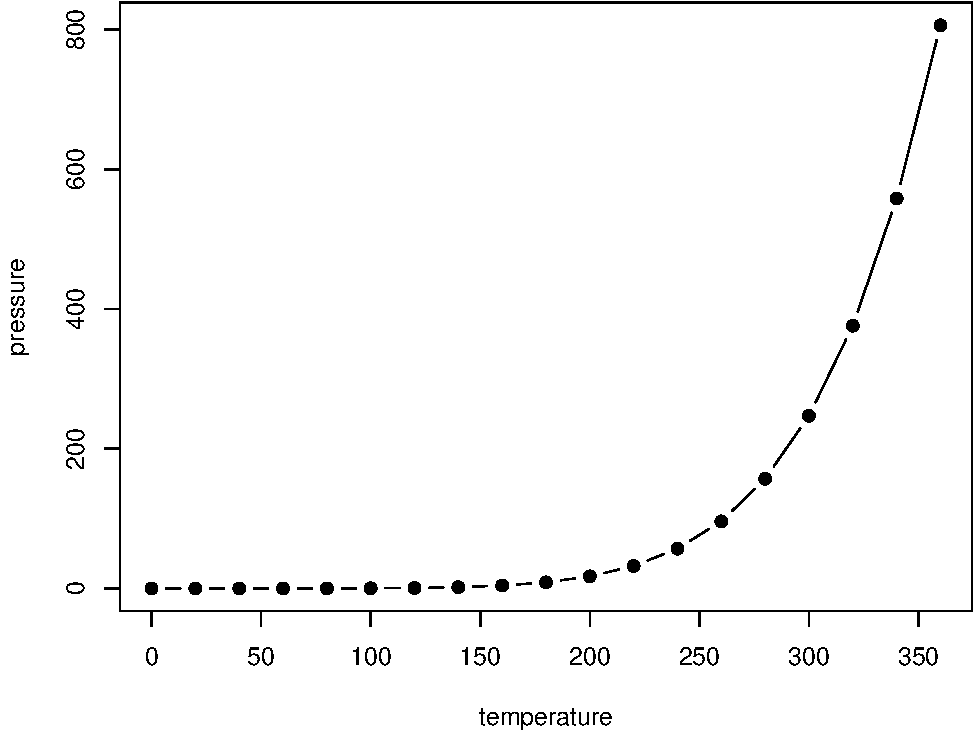
\includegraphics[width=0.8\linewidth]{202401280000-minimal-book-example_files/figure-latex/nice-fig-1} 

}

\caption{Here is a nice figure!}\label{fig:nice-fig}
\end{figure}

Don't miss Table \ref{tab:nice-tab}.

\begin{Shaded}
\begin{Highlighting}[]
\NormalTok{knitr}\SpecialCharTok{::}\FunctionTok{kable}\NormalTok{(}
  \FunctionTok{head}\NormalTok{(pressure, }\DecValTok{10}\NormalTok{), }\AttributeTok{caption =} \StringTok{\textquotesingle{}Here is a nice table!\textquotesingle{}}\NormalTok{,}
  \AttributeTok{booktabs =} \ConstantTok{TRUE}
\NormalTok{)}
\end{Highlighting}
\end{Shaded}

\begin{table}

\caption{\label{tab:nice-tab}Here is a nice table!}
\centering
\begin{tabular}[t]{rr}
\toprule
temperature & pressure\\
\midrule
0 & 0.0002\\
20 & 0.0012\\
40 & 0.0060\\
60 & 0.0300\\
80 & 0.0900\\
\addlinespace
100 & 0.2700\\
120 & 0.7500\\
140 & 1.8500\\
160 & 4.2000\\
180 & 8.8000\\
\bottomrule
\end{tabular}
\end{table}

\section{Parts}\label{parts}

You can add parts to organize one or more book chapters together. Parts can be inserted at the top of an .Rmd file, before the first-level chapter heading in that same file.

Add a numbered part: \texttt{\#\ (PART)\ Act\ one\ \{-\}} (followed by \texttt{\#\ A\ chapter})

Add an unnumbered part: \texttt{\#\ (PART\textbackslash{}*)\ Act\ one\ \{-\}} (followed by \texttt{\#\ A\ chapter})

Add an appendix as a special kind of un-numbered part: \texttt{\#\ (APPENDIX)\ Other\ stuff\ \{-\}} (followed by \texttt{\#\ A\ chapter}). Chapters in an appendix are prepended with letters instead of numbers.

\section{Footnotes and citations}\label{footnotes-and-citations}

\subsection{Footnotes}\label{footnotes}

Footnotes are put inside the square brackets after a caret \texttt{\^{}{[}{]}}. Like this one \footnote{This is a footnote.}.

\subsection{Citations}\label{citations}

Reference items in your bibliography file(s) using \texttt{@key}.

For example, we are using the \textbf{bookdown} package\textsuperscript{\citeproc{ref-R-bookdown}{1}} (check out the last code chunk in index.Rmd to see how this citation key was added) in this sample book, which was built on top of R Markdown and \textbf{knitr}\textsuperscript{\citeproc{ref-xie2015}{2}} (this citation was added manually in an external file book.bib).
Note that the \texttt{.bib} files need to be listed in the index.Rmd with the YAML \texttt{bibliography} key.

The RStudio Visual Markdown Editor can also make it easier to insert citations: \url{https://rstudio.github.io/visual-markdown-editing/\#/citations}

\section{Blocks}\label{blocks}

\subsection{Equations}\label{equations}

Here is an equation.

\begin{equation} 
  f\left(k\right) = \binom{n}{k} p^k\left(1-p\right)^{n-k}
  \label{eq:binom}
\end{equation}

You may refer to using \texttt{\textbackslash{}@ref(eq:binom)}, like see Equation \eqref{eq:binom}.

\subsection{Theorems and proofs}\label{theorems-and-proofs}

Labeled theorems can be referenced in text using \texttt{\textbackslash{}@ref(thm:tri)}, for example, check out this smart theorem \ref{thm:tri}.

\begin{theorem}
\protect\hypertarget{thm:tri}{}\label{thm:tri}For a right triangle, if \(c\) denotes the \emph{length} of the hypotenuse
and \(a\) and \(b\) denote the lengths of the \textbf{other} two sides, we have
\[a^2 + b^2 = c^2\]
\end{theorem}

Read more here \url{https://bookdown.org/yihui/bookdown/markdown-extensions-by-bookdown.html}.

\subsection{Callout blocks}\label{callout-blocks}

The R Markdown Cookbook provides more help on how to use custom blocks to design your own callouts: \url{https://bookdown.org/yihui/rmarkdown-cookbook/custom-blocks.html}

\section{Sharing your book}\label{sharing-your-book}

\subsection{Publishing}\label{publishing}

HTML books can be published online, see: \url{https://bookdown.org/yihui/bookdown/publishing.html}

\subsection{404 pages}\label{pages}

By default, users will be directed to a 404 page if they try to access a webpage that cannot be found. If you'd like to customize your 404 page instead of using the default, you may add either a \texttt{\_404.Rmd} or \texttt{\_404.md} file to your project root and use code and/or Markdown syntax.

\subsection{Metadata for sharing}\label{metadata-for-sharing}

Bookdown HTML books will provide HTML metadata for social sharing on platforms like Twitter, Facebook, and LinkedIn, using information you provide in the \texttt{index.Rmd} YAML. To setup, set the \texttt{url} for your book and the path to your \texttt{cover-image} file. Your book's \texttt{title} and \texttt{description} are also used.

This \texttt{gitbook} uses the same social sharing data across all chapters in your book- all links shared will look the same.

Specify your book's source repository on GitHub using the \texttt{edit} key under the configuration options in the \texttt{\_output.yml} file, which allows users to suggest an edit by linking to a chapter's source file.

Read more about the features of this output format here:

\url{https://pkgs.rstudio.com/bookdown/reference/gitbook.html}

Or use:

\begin{Shaded}
\begin{Highlighting}[]
\NormalTok{?bookdown}\SpecialCharTok{::}\NormalTok{gitbook}
\end{Highlighting}
\end{Shaded}

\chapter{test}\label{test}

\section{RStudio}\label{rstudio}

\subsection{writer options}\label{writer-options}

\url{https://rstudio.github.io/visual-markdown-editing/markdown.html\#writer-options}

\subsubsection{line wrapping}\label{line-wrapping}

\url{https://rstudio.github.io/visual-markdown-editing/markdown.html\#line-wrapping}

\subsubsection{ensuring the same markdown between source / visual mode}\label{ensuring-the-same-markdown-between-source-visual-mode}

\url{https://stackoverflow.com/questions/71775027/rstudio-switch-markdown-editing-mode-between-source-and-visual-changes-special}

\textbf{canonical mode}

\url{https://rstudio.github.io/visual-markdown-editing/markdown.html\#canonical-mode}

\begin{Shaded}
\begin{Highlighting}[]
\PreprocessorTok{{-}{-}{-}}
\FunctionTok{title}\KeywordTok{:}\AttributeTok{ }\StringTok{"My Document"}
\FunctionTok{editor\_options}\KeywordTok{:}
\AttributeTok{  }\FunctionTok{markdown}\KeywordTok{:}
\AttributeTok{    }\FunctionTok{wrap}\KeywordTok{:}\AttributeTok{ }\DecValTok{72}
\AttributeTok{    }\FunctionTok{references}\KeywordTok{:}\AttributeTok{ }
\AttributeTok{      }\FunctionTok{location}\KeywordTok{:}\AttributeTok{ block}
\AttributeTok{    }\FunctionTok{canonical}\KeywordTok{:}\AttributeTok{ }\CharTok{true}
\PreprocessorTok{{-}{-}{-}}
\end{Highlighting}
\end{Shaded}

\subsection{Rtools}\label{rtools}

Rtools43 for Windows
\url{https://cran.r-project.org/bin/windows/Rtools/rtools43/rtools.html}

\subsection{addins}\label{addins}

\url{https://github.com/rstudio/addinexamples}

\begin{verbatim}
if (!requireNamespace("devtools", quietly = TRUE))
  install.packages("devtools")
  
devtools::install_github("rstudio/htmltools")
devtools::install_github("rstudio/shiny")
devtools::install_github("rstudio/miniUI")
\end{verbatim}

\subsection{Git}\label{git}

commit: filename or extension is too long

\url{https://stackoverflow.com/questions/22575662/filename-too-long-in-git-for-windows}

\url{https://stackoverflow.com/questions/55327408/how-to-fix-git-for-windows-error-could-not-lock-config-file-c-file-path-to-g}

\section{RMarkdown}\label{rmarkdown}

\begin{CJK}{UTF8}{bsmi}
R Markdown 指南 https://cosname.github.io/rmarkdown-guide/index.html
\end{CJK}

\url{https://www.rstudio.com/wp-content/uploads/2015/02/rmarkdown-cheatsheet.pdf}

\url{https://slides.yihui.org/2020-taipei-satrday-rmarkdown.html\#1}

\subsection{verbatim}\label{verbatim}

\url{https://community.rstudio.com/t/continued-issues-with-new-verbatim-in-rstudio/139737}

\url{https://bookdown.org/yihui/rmarkdown-cookbook/verbatim-code-chunks.html}

\subsection{Pandoc link}\label{pandoc-link}

\url{https://pandoc.org/chunkedhtml-demo/8.16-links-1.html}

\url{https://stackoverflow.com/questions/39281266/use-internal-links-in-rmarkdown-html-output}

\url{https://community.rstudio.com/t/how-to-hyperlink-between-different-rmd-files-in-rmarkdown/62289}

\subsection{URL}\label{url}

\url{https://stackoverflow.com/questions/29787850/how-do-i-add-a-url-to-r-markdown}

\begin{verbatim}
[I'm an inline-style link](https://www.google.com)

[I'm an inline-style link with title](https://www.google.com "Google's Homepage")

[I'm a reference-style link][Arbitrary case-insensitive reference text]

[I'm a relative reference to a repository file](../blob/master/LICENSE)

[You can use numbers for reference-style link definitions][1]

Or leave it empty and use the [link text itself]

Some text to show that the reference links can follow later.

[arbitrary case-insensitive reference text]: https://www.mozilla.org
[1]: http://slashdot.org
[link text itself]: http://www.reddit.com
\end{verbatim}

\subsection{arrow}\label{arrow}

\url{https://reimbar.org/dev/arrows/}

Up arrow: \texttt{\&uarr;}

Down arrow: \texttt{\&darr;}

Left arrow: \texttt{\&larr;}

Right arrow: \texttt{\&rarr;}

Double headed arrow: \texttt{\&harr;}

\subsection{superscript and subscript}\label{superscript-and-subscript}

script\textsuperscript{superscript}\textsubscript{subscript}

\begin{Shaded}
\begin{Highlighting}[]
\NormalTok{script\^{}superscript\^{}}
\end{Highlighting}
\end{Shaded}

script\textsuperscript{superscript}

\begin{Shaded}
\begin{Highlighting}[]
\NormalTok{\textasciitilde{}subscript\textasciitilde{}}
\end{Highlighting}
\end{Shaded}

script\textsubscript{subscript}

\subsubsection{LaTeX}\label{latex}

\url{https://tex.stackexchange.com/questions/580824/subscript-not-distinguished-enough}

\url{https://tex.stackexchange.com/questions/262295/make-subscript-size-smaller-always}

\subsection{equation}\label{equation}

\url{https://stackoverflow.com/questions/26049762/erroneous-nesting-of-equation-structures-in-using-beginalign-in-a-multi-l}

\subsubsection{proof QED}\label{proof-qed}

\url{https://math.meta.stackexchange.com/questions/3582/qed-for-mathjax-here-on-stackexchange}

\texttt{\textbackslash{}tag*\{\$\textbackslash{}Box\$\}}

\[
a^2+b^2=c^2 \tag*{$\Box$}
\]

\texttt{\textbackslash{}tag*\{\$\textbackslash{}blacksquare\$\}}

\[
a^2+b^2=c^2 \tag*{$\blacksquare$}
\]

\subsection{image}\label{image}

\url{https://stackoverflow.com/questions/25166624/insert-picture-table-in-r-markdown}

\subsubsection{DiagrammeR / mermaid flowchart}\label{diagrammer-mermaid-flowchart}

\begin{verbatim}
Error: Functions that produce HTML output found in document targeting latex output.
Please change the output type of this document to HTML.
If your aiming to have some HTML widgets shown in non-HTML format as a screenshot,
please install webshot or webshot2 R package for knitr to do the screenshot.
Alternatively, you can allow HTML output in non-HTML formats
by adding this option to the YAML front-matter of
your rmarkdown file:

  always_allow_html: true

Note however that the HTML output will not be visible in non-HTML formats.
\end{verbatim}

\url{https://bookdown.org/yihui/rmarkdown-cookbook/diagrams.html\#diagrams}

\url{https://stackoverflow.com/questions/40803017/how-to-include-diagrammer-mermaid-flowchart-in-a-rmarkdown-file}

\begin{verbatim}
{r}
library(DiagrammeR)
mermaid("
graph LR
    A-->B
",
width = 100
)
\end{verbatim}

\url{https://github.com/rich-iannone/DiagrammeR/issues/364}

\url{https://stackoverflow.com/questions/55994210/how-to-solve-diagrammer-waste-of-space-issue-in-rmarkdown}

\subsubsection{multiple images / figures in the same line}\label{multiple-images-figures-in-the-same-line}

\url{https://cosname.github.io/rmarkdown-guide/rmarkdown-base.html\#element-figure}

\begin{verbatim}
{r, fig.show = "hold", out.width = "50%"}
plot(cars)
plot(nhtemp)
\end{verbatim}

\begin{Shaded}
\begin{Highlighting}[]
\FunctionTok{plot}\NormalTok{(cars)}
\FunctionTok{plot}\NormalTok{(nhtemp)}
\end{Highlighting}
\end{Shaded}

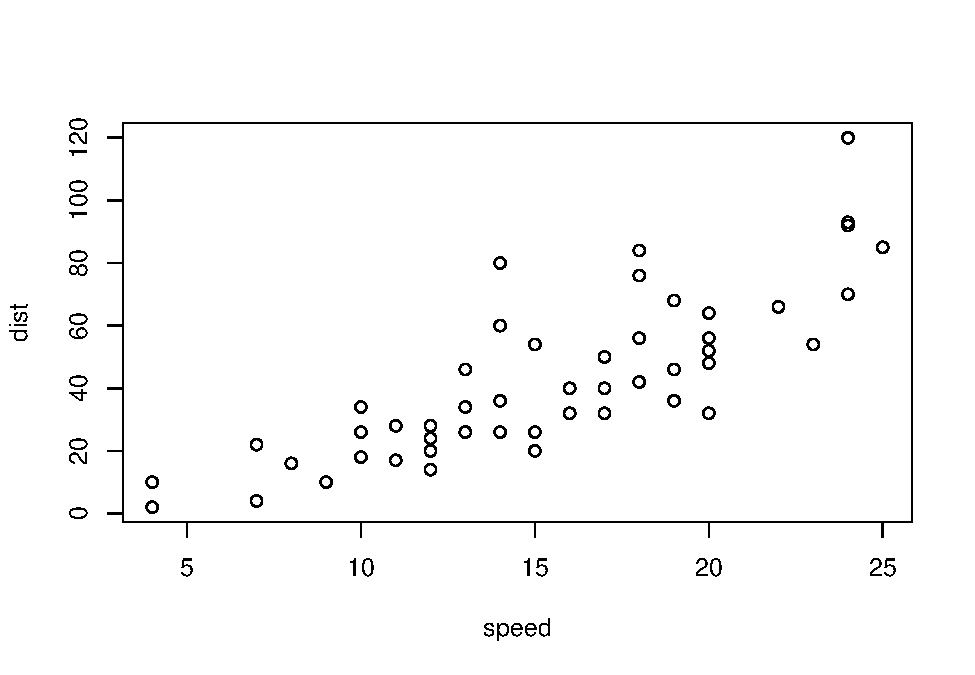
\includegraphics[width=0.5\linewidth]{202401280001-test_files/figure-latex/unnamed-chunk-4-1} 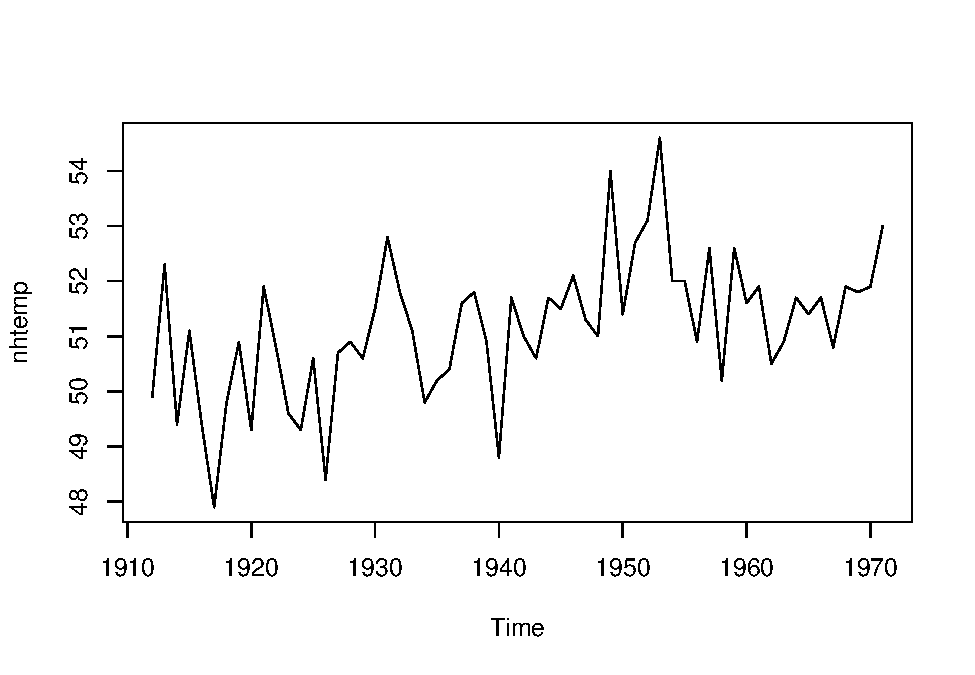
\includegraphics[width=0.5\linewidth]{202401280001-test_files/figure-latex/unnamed-chunk-4-2}

cf.

\begin{verbatim}
{r}
plot(cars)
plot(nhtemp)
\end{verbatim}

\begin{Shaded}
\begin{Highlighting}[]
\FunctionTok{plot}\NormalTok{(cars)}
\end{Highlighting}
\end{Shaded}

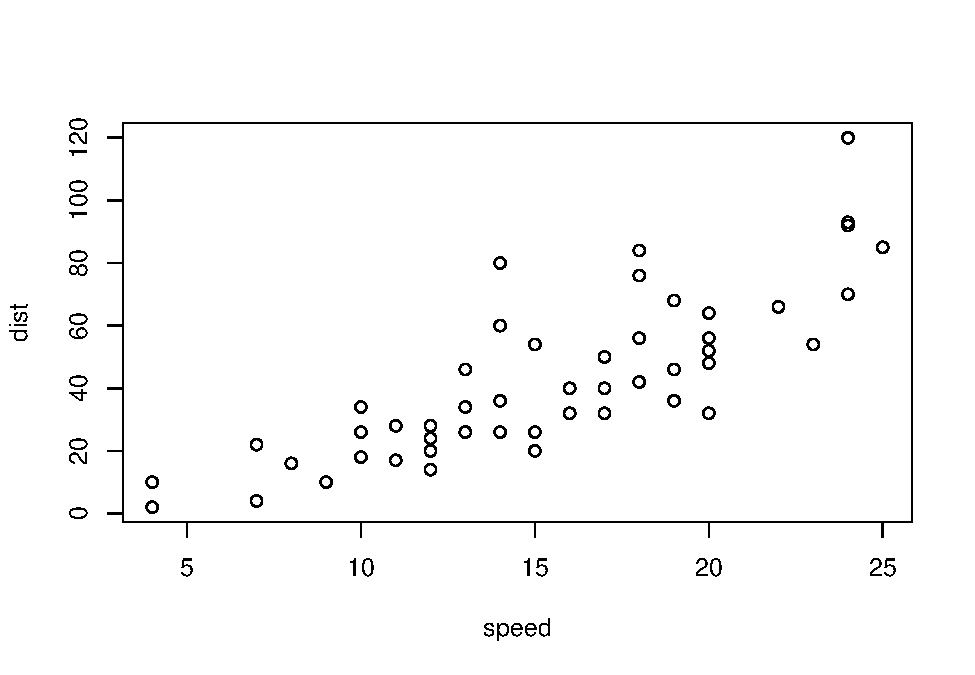
\includegraphics{202401280001-test_files/figure-latex/unnamed-chunk-5-1.pdf}

\begin{Shaded}
\begin{Highlighting}[]
\FunctionTok{plot}\NormalTok{(nhtemp)}
\end{Highlighting}
\end{Shaded}

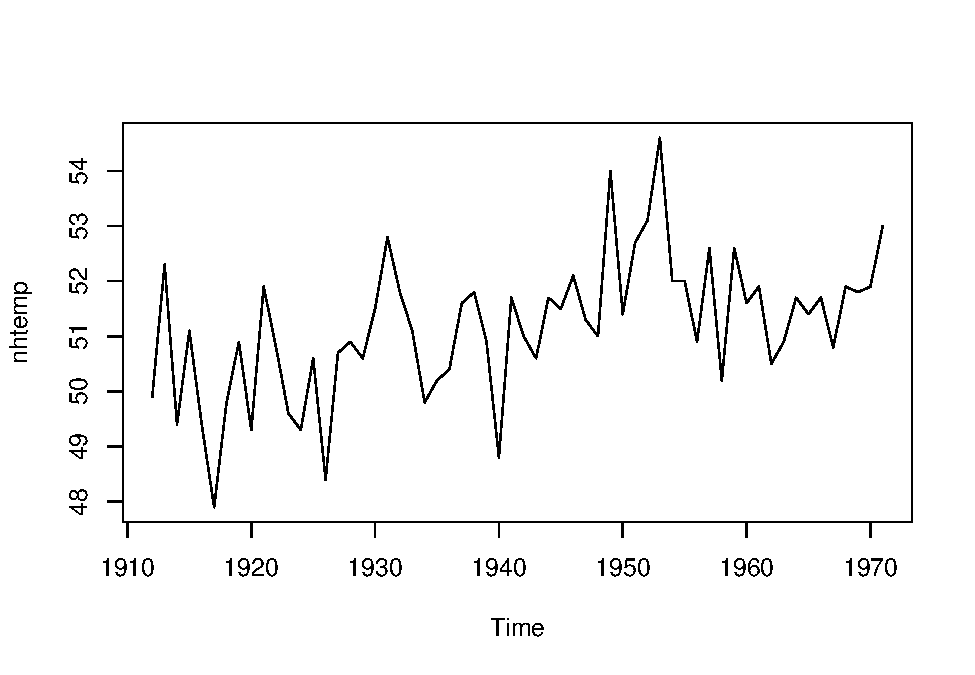
\includegraphics{202401280001-test_files/figure-latex/unnamed-chunk-5-2.pdf}

\subsubsection{figure size}\label{figure-size}

\url{https://sebastiansauer.github.io/figure_sizing_knitr/}

YAML in index.Rmd

\begin{Shaded}
\begin{Highlighting}[]
\PreprocessorTok{{-}{-}{-} }
\FunctionTok{title}\KeywordTok{:}\AttributeTok{ }\StringTok{"My Document"}\AttributeTok{ }
\FunctionTok{output}\KeywordTok{:}\AttributeTok{ html\_document: }
\FunctionTok{fig\_width}\KeywordTok{:}\AttributeTok{ }\DecValTok{6}\AttributeTok{ }
\FunctionTok{fig\_height}\KeywordTok{:}\AttributeTok{ }\DecValTok{4}\AttributeTok{ }
\PreprocessorTok{{-}{-}{-} }
\end{Highlighting}
\end{Shaded}

first R-chunk in your RMD document

\begin{verbatim}
knitr::opts_chunk$set(fig.width=12, fig.height=8) 
\end{verbatim}

width, height and options

\texttt{\textasciigrave{}\textasciigrave{}\textasciigrave{}\{r\ fig.height\ =\ 3,\ fig.width\ =\ 5}

\texttt{plot(pressure)}

\texttt{\textasciigrave{}\textasciigrave{}\textasciigrave{}}

\texttt{\{r\ fig.height\ =\ 3,\ fig.width\ =\ 5}

\begin{Shaded}
\begin{Highlighting}[]
\FunctionTok{plot}\NormalTok{(pressure)}
\end{Highlighting}
\end{Shaded}

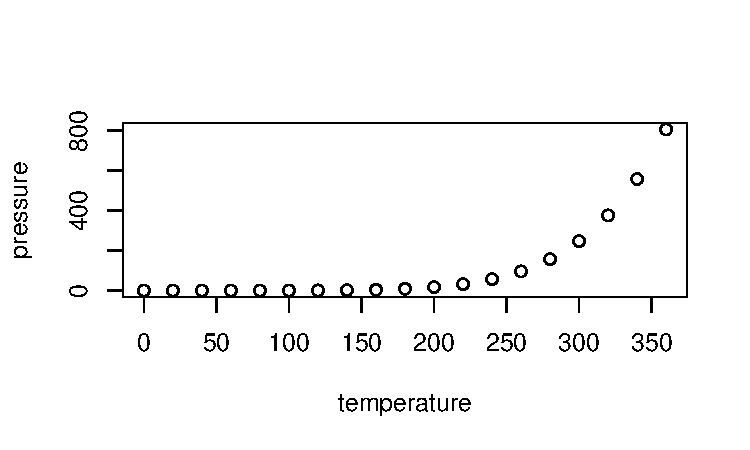
\includegraphics{202401280001-test_files/figure-latex/unnamed-chunk-7-1.pdf}

\texttt{\{r\ fig.height\ =\ 3,\ fig.width\ =\ 3,\ fig.align\ =\ "center"}

\begin{Shaded}
\begin{Highlighting}[]
\FunctionTok{plot}\NormalTok{(pressure)}
\end{Highlighting}
\end{Shaded}

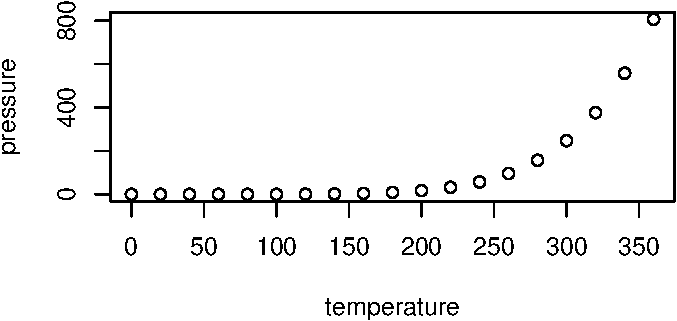
\includegraphics{202401280001-test_files/figure-latex/unnamed-chunk-8-1.pdf}

\texttt{\{r\ fig.width\ =\ 5,\ fig.asp\ =\ .62}

\begin{Shaded}
\begin{Highlighting}[]
\FunctionTok{plot}\NormalTok{(pressure)}
\end{Highlighting}
\end{Shaded}

\begin{center}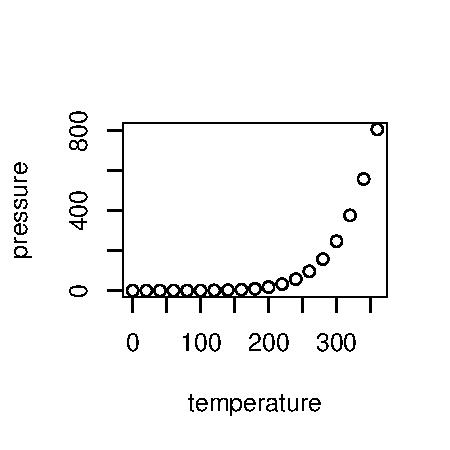
\includegraphics{202401280001-test_files/figure-latex/unnamed-chunk-9-1} \end{center}

\begin{Shaded}
\begin{Highlighting}[]
\DataTypeTok{\textless{}}\KeywordTok{center}\DataTypeTok{\textgreater{}}
\AlertTok{![](https://bookdown.org/yihui/rmarkdown{-}cookbook/images/cover.png)}\NormalTok{\{width=20\%\}}
\DataTypeTok{\textless{}/}\KeywordTok{center}\DataTypeTok{\textgreater{}}
\end{Highlighting}
\end{Shaded}

\paragraph{\texorpdfstring{\texttt{knitr}}{knitr}}\label{knitr}

\url{https://yihui.org/knitr/options/}

\url{https://bookdown.org/yihui/rmarkdown/tufte-figures.html}

\begin{Shaded}
\begin{Highlighting}[]
\FunctionTok{par}\NormalTok{(}\AttributeTok{mar =} \FunctionTok{c}\NormalTok{(}\DecValTok{4}\NormalTok{, }\DecValTok{4}\NormalTok{, .}\DecValTok{1}\NormalTok{, .}\DecValTok{2}\NormalTok{)); }\FunctionTok{plot}\NormalTok{(sunspots)}
\end{Highlighting}
\end{Shaded}

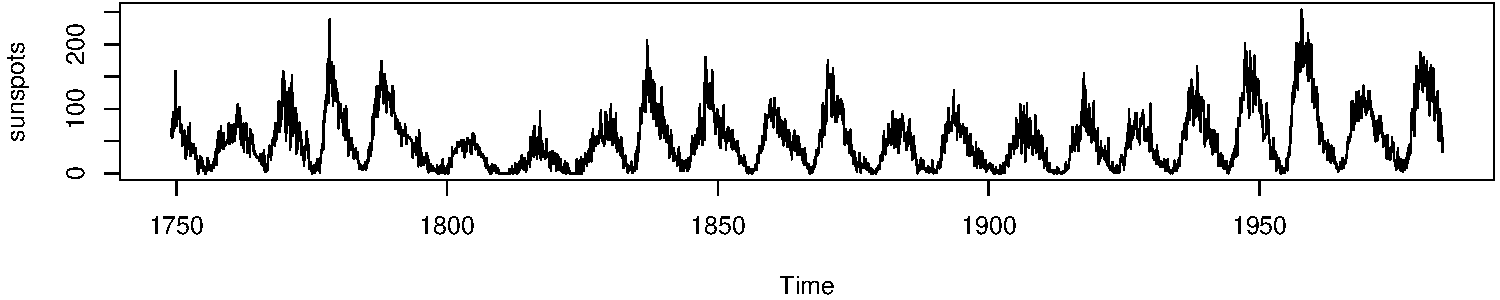
\includegraphics{202401280001-test_files/figure-latex/unnamed-chunk-11-1.pdf}

\begin{Shaded}
\begin{Highlighting}[]
\FunctionTok{plot}\NormalTok{(cars)}
\end{Highlighting}
\end{Shaded}

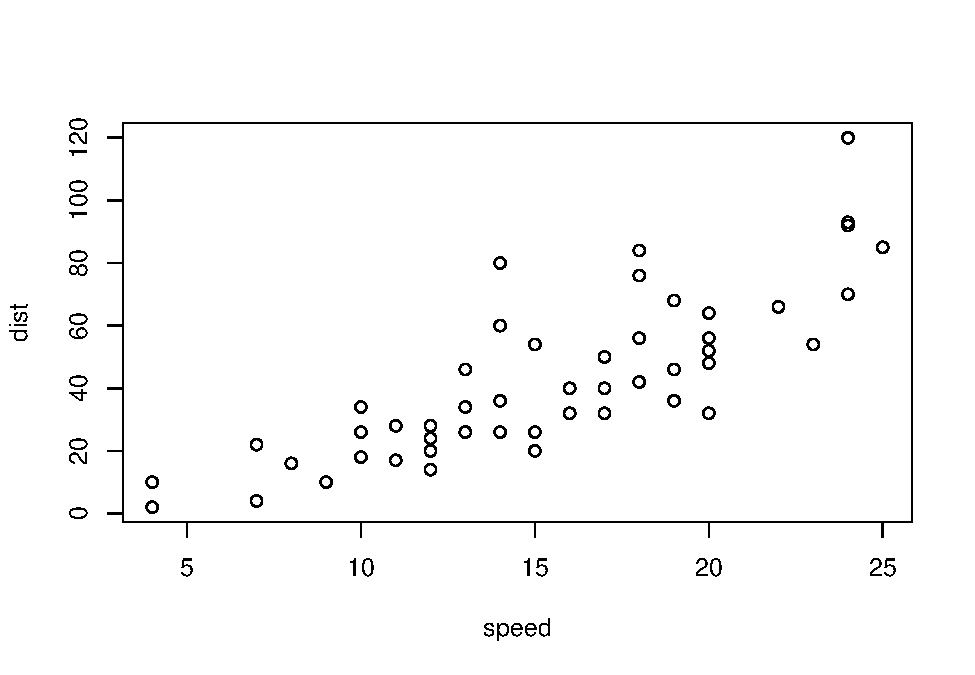
\includegraphics{202401280001-test_files/figure-latex/fig-margin-1.pdf}

\begin{Shaded}
\begin{Highlighting}[]
\NormalTok{We know from \_the first fundamental theorem of calculus\_ that}
\NormalTok{for $x$ in $[a, b]$:}
\NormalTok{$$\textbackslash{}frac\{d\}\{dx\}\textbackslash{}left( \textbackslash{}int\_\{a\}\^{}\{x\} f(u)\textbackslash{},du\textbackslash{}right)=f(x).$$}
\end{Highlighting}
\end{Shaded}

\paragraph{\texorpdfstring{\texttt{out.width} vs.~\texttt{fig.width}}{out.width vs.~fig.width}}\label{out.width-vs.-fig.width}

\url{https://stackoverflow.com/questions/29657777/how-to-make-fig-width-and-out-width-consistent-with-knitr}

when chunk option \texttt{cache=FALSE} is set, then \texttt{out.width} has no effect because no PDF output is created. Hence one has to specify exact measures in inches for \texttt{fig.width} and \texttt{fig.height} for each chunk

\url{https://stackoverflow.com/questions/59567235/a-ggmap-too-small-when-rendered-within-a-rmd-file}

\begin{center}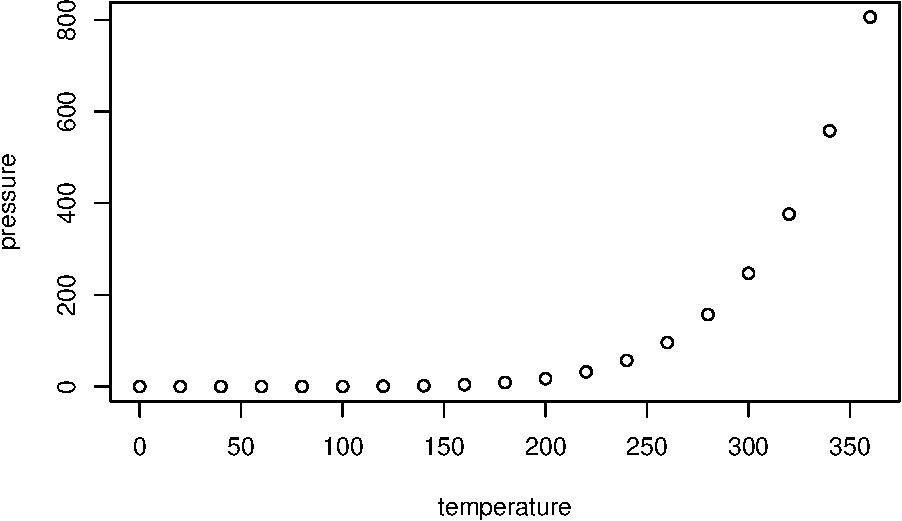
\includegraphics[width=1\linewidth]{202401280001-test_files/figure-latex/unnamed-chunk-13-1} \end{center}

\begin{Shaded}
\begin{Highlighting}[]
\FunctionTok{plot}\NormalTok{(pressure)}
\end{Highlighting}
\end{Shaded}

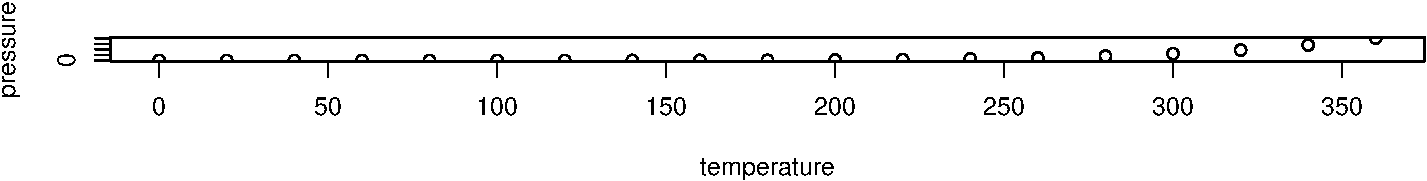
\includegraphics{202401280001-test_files/figure-latex/unnamed-chunk-14-1.pdf}

problem: \texttt{out.width=\textquotesingle{}100\%\textquotesingle{}} causing \texttt{LaTeX\ Error:\ Not\ in\ outer\ par\ mode.}

solution: \texttt{out.width=if\ (knitr:::is\_html\_output())\ \textquotesingle{}100\%\textquotesingle{}}

\begin{cols}

\begin{col}{0.4\textwidth}

\begin{Shaded}
\begin{Highlighting}[]
\KeywordTok{\textbackslash{}begin}\NormalTok{\{}\ExtensionTok{tikzpicture}\NormalTok{\}}
  \FunctionTok{\textbackslash{}draw}\NormalTok{ ({-}1,1){-}{-}(0,0){-}{-}(1,2);}
\KeywordTok{\textbackslash{}end}\NormalTok{\{}\ExtensionTok{tikzpicture}\NormalTok{\}}
\end{Highlighting}
\end{Shaded}

\end{col}

\begin{col}{0.05\textwidth}
~


\end{col}

\begin{col}{0.55\textwidth}
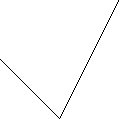
\includegraphics{202401280001-test_files/figure-latex/unnamed-chunk-16-1.pdf}

\end{col}

\end{cols}

\texttt{fig.width=10,\ fig.height=2}

\begin{cols}

\begin{col}{0.4\textwidth}

\begin{Shaded}
\begin{Highlighting}[]
\KeywordTok{\textbackslash{}begin}\NormalTok{\{}\ExtensionTok{tikzpicture}\NormalTok{\}}
  \FunctionTok{\textbackslash{}draw}\NormalTok{ ({-}1,1){-}{-}(0,0){-}{-}(1,2);}
\KeywordTok{\textbackslash{}end}\NormalTok{\{}\ExtensionTok{tikzpicture}\NormalTok{\}}
\end{Highlighting}
\end{Shaded}

\end{col}

\begin{col}{0.05\textwidth}
~


\end{col}

\begin{col}{0.55\textwidth}
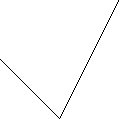
\includegraphics{202401280001-test_files/figure-latex/unnamed-chunk-18-1.pdf}

\end{col}

\end{cols}

\texttt{out.width=if\ (knitr:::is\_html\_output())\ \textquotesingle{}100\%\textquotesingle{}}

\begin{cols}

\begin{col}{0.4\textwidth}

\begin{Shaded}
\begin{Highlighting}[]
\KeywordTok{\textbackslash{}begin}\NormalTok{\{}\ExtensionTok{tikzpicture}\NormalTok{\}}
  \FunctionTok{\textbackslash{}draw}\NormalTok{ ({-}1,1){-}{-}(0,0){-}{-}(1,2);}
\KeywordTok{\textbackslash{}end}\NormalTok{\{}\ExtensionTok{tikzpicture}\NormalTok{\}}
\end{Highlighting}
\end{Shaded}

\end{col}

\begin{col}{0.05\textwidth}
~


\end{col}

\begin{col}{0.55\textwidth}
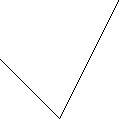
\includegraphics{202401280001-test_files/figure-latex/unnamed-chunk-20-1.pdf}

\end{col}

\end{cols}

\subsubsection{dynamic knitr plot width and height}\label{dynamic-knitr-plot-width-and-height}

\url{https://stackoverflow.com/questions/15365829/dynamic-height-and-width-for-knitr-plots}

\begin{Shaded}
\begin{Highlighting}[]
\FunctionTok{plot}\NormalTok{(pressure)}
\end{Highlighting}
\end{Shaded}

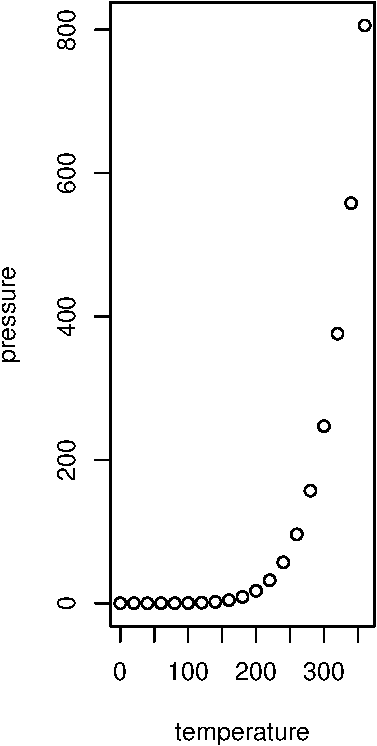
\includegraphics{202401280001-test_files/figure-latex/unnamed-chunk-22-1.pdf}

\subsubsection{web image in PDF}\label{web-image-in-pdf}

\url{https://stackoverflow.com/questions/46331896/how-can-i-insert-an-image-from-internet-to-the-pdf-file-produced-by-r-bookdown-i}

\begin{verbatim}
cover_url = 'https://bookdown.org/yihui/bookdown/images/cover.jpg'
if (!file.exists(cover_file <- xfun::url_filename(cover_url)))
  xfun::download_file(cover_url)
knitr::include_graphics(if (knitr::pandoc_to('html')) cover_url else cover_file)
\end{verbatim}

\begin{figure}
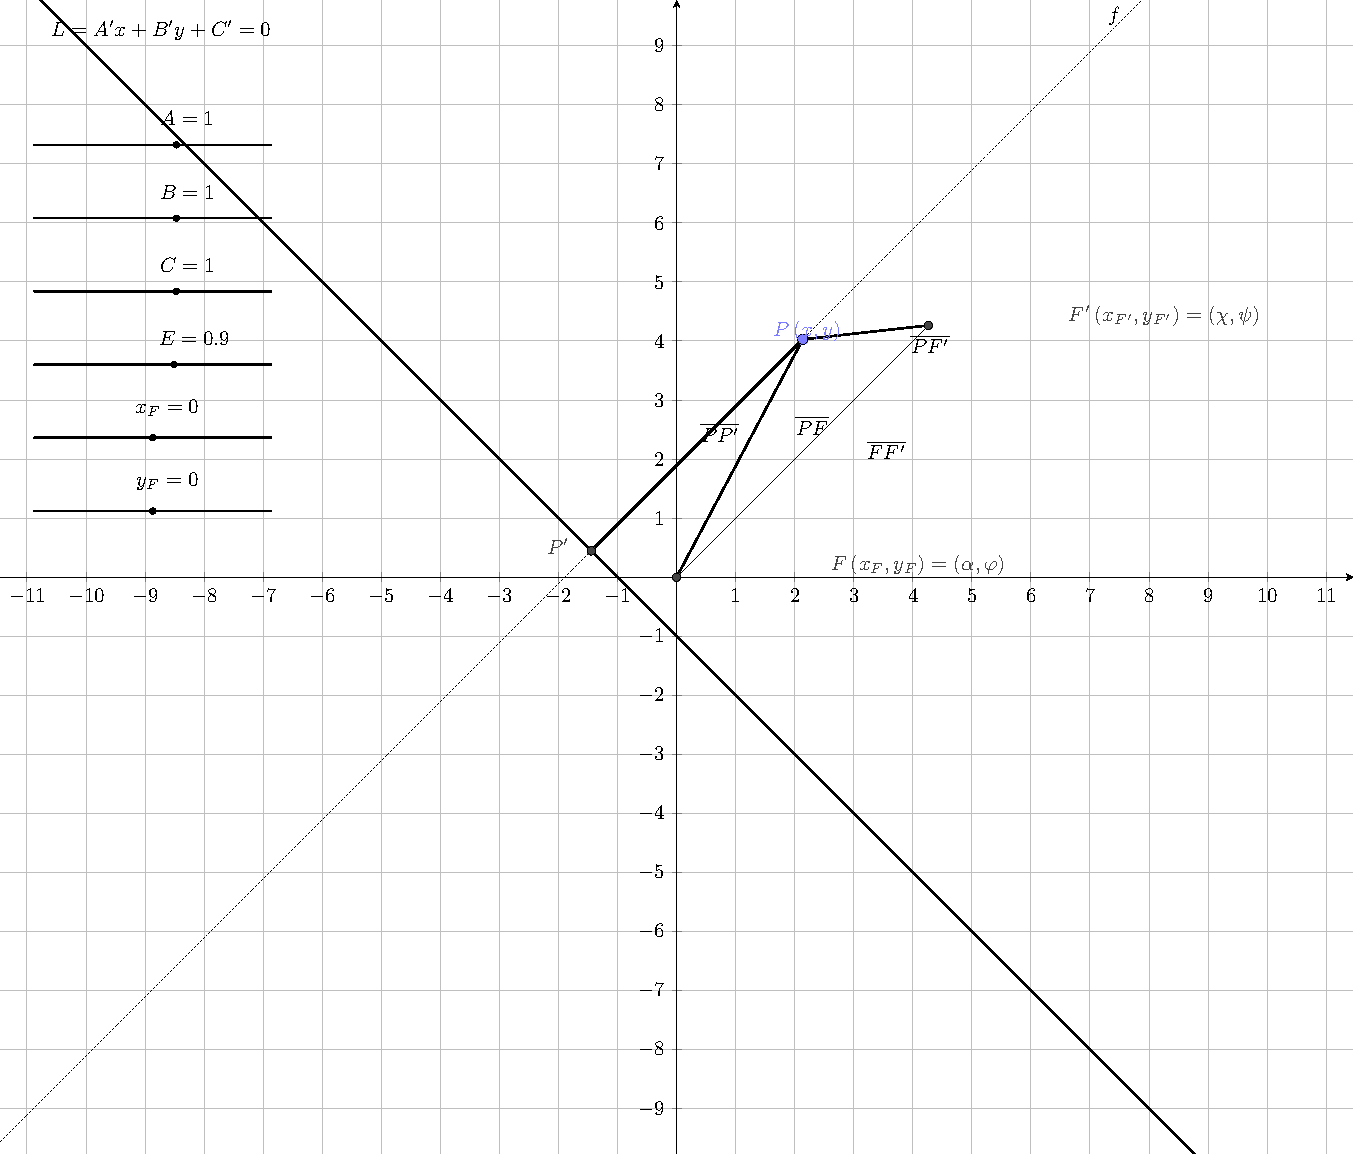
\includegraphics[width=0.75\linewidth]{202401280001-test_files/figure-latex/unnamed-chunk-24-1} \caption{conic sections}\label{fig:unnamed-chunk-24}
\end{figure}

\subsubsection{SVG}\label{svg}

\url{https://stackoverflow.com/questions/50165404/how-to-make-a-pdf-using-bookdown-including-svg-images}

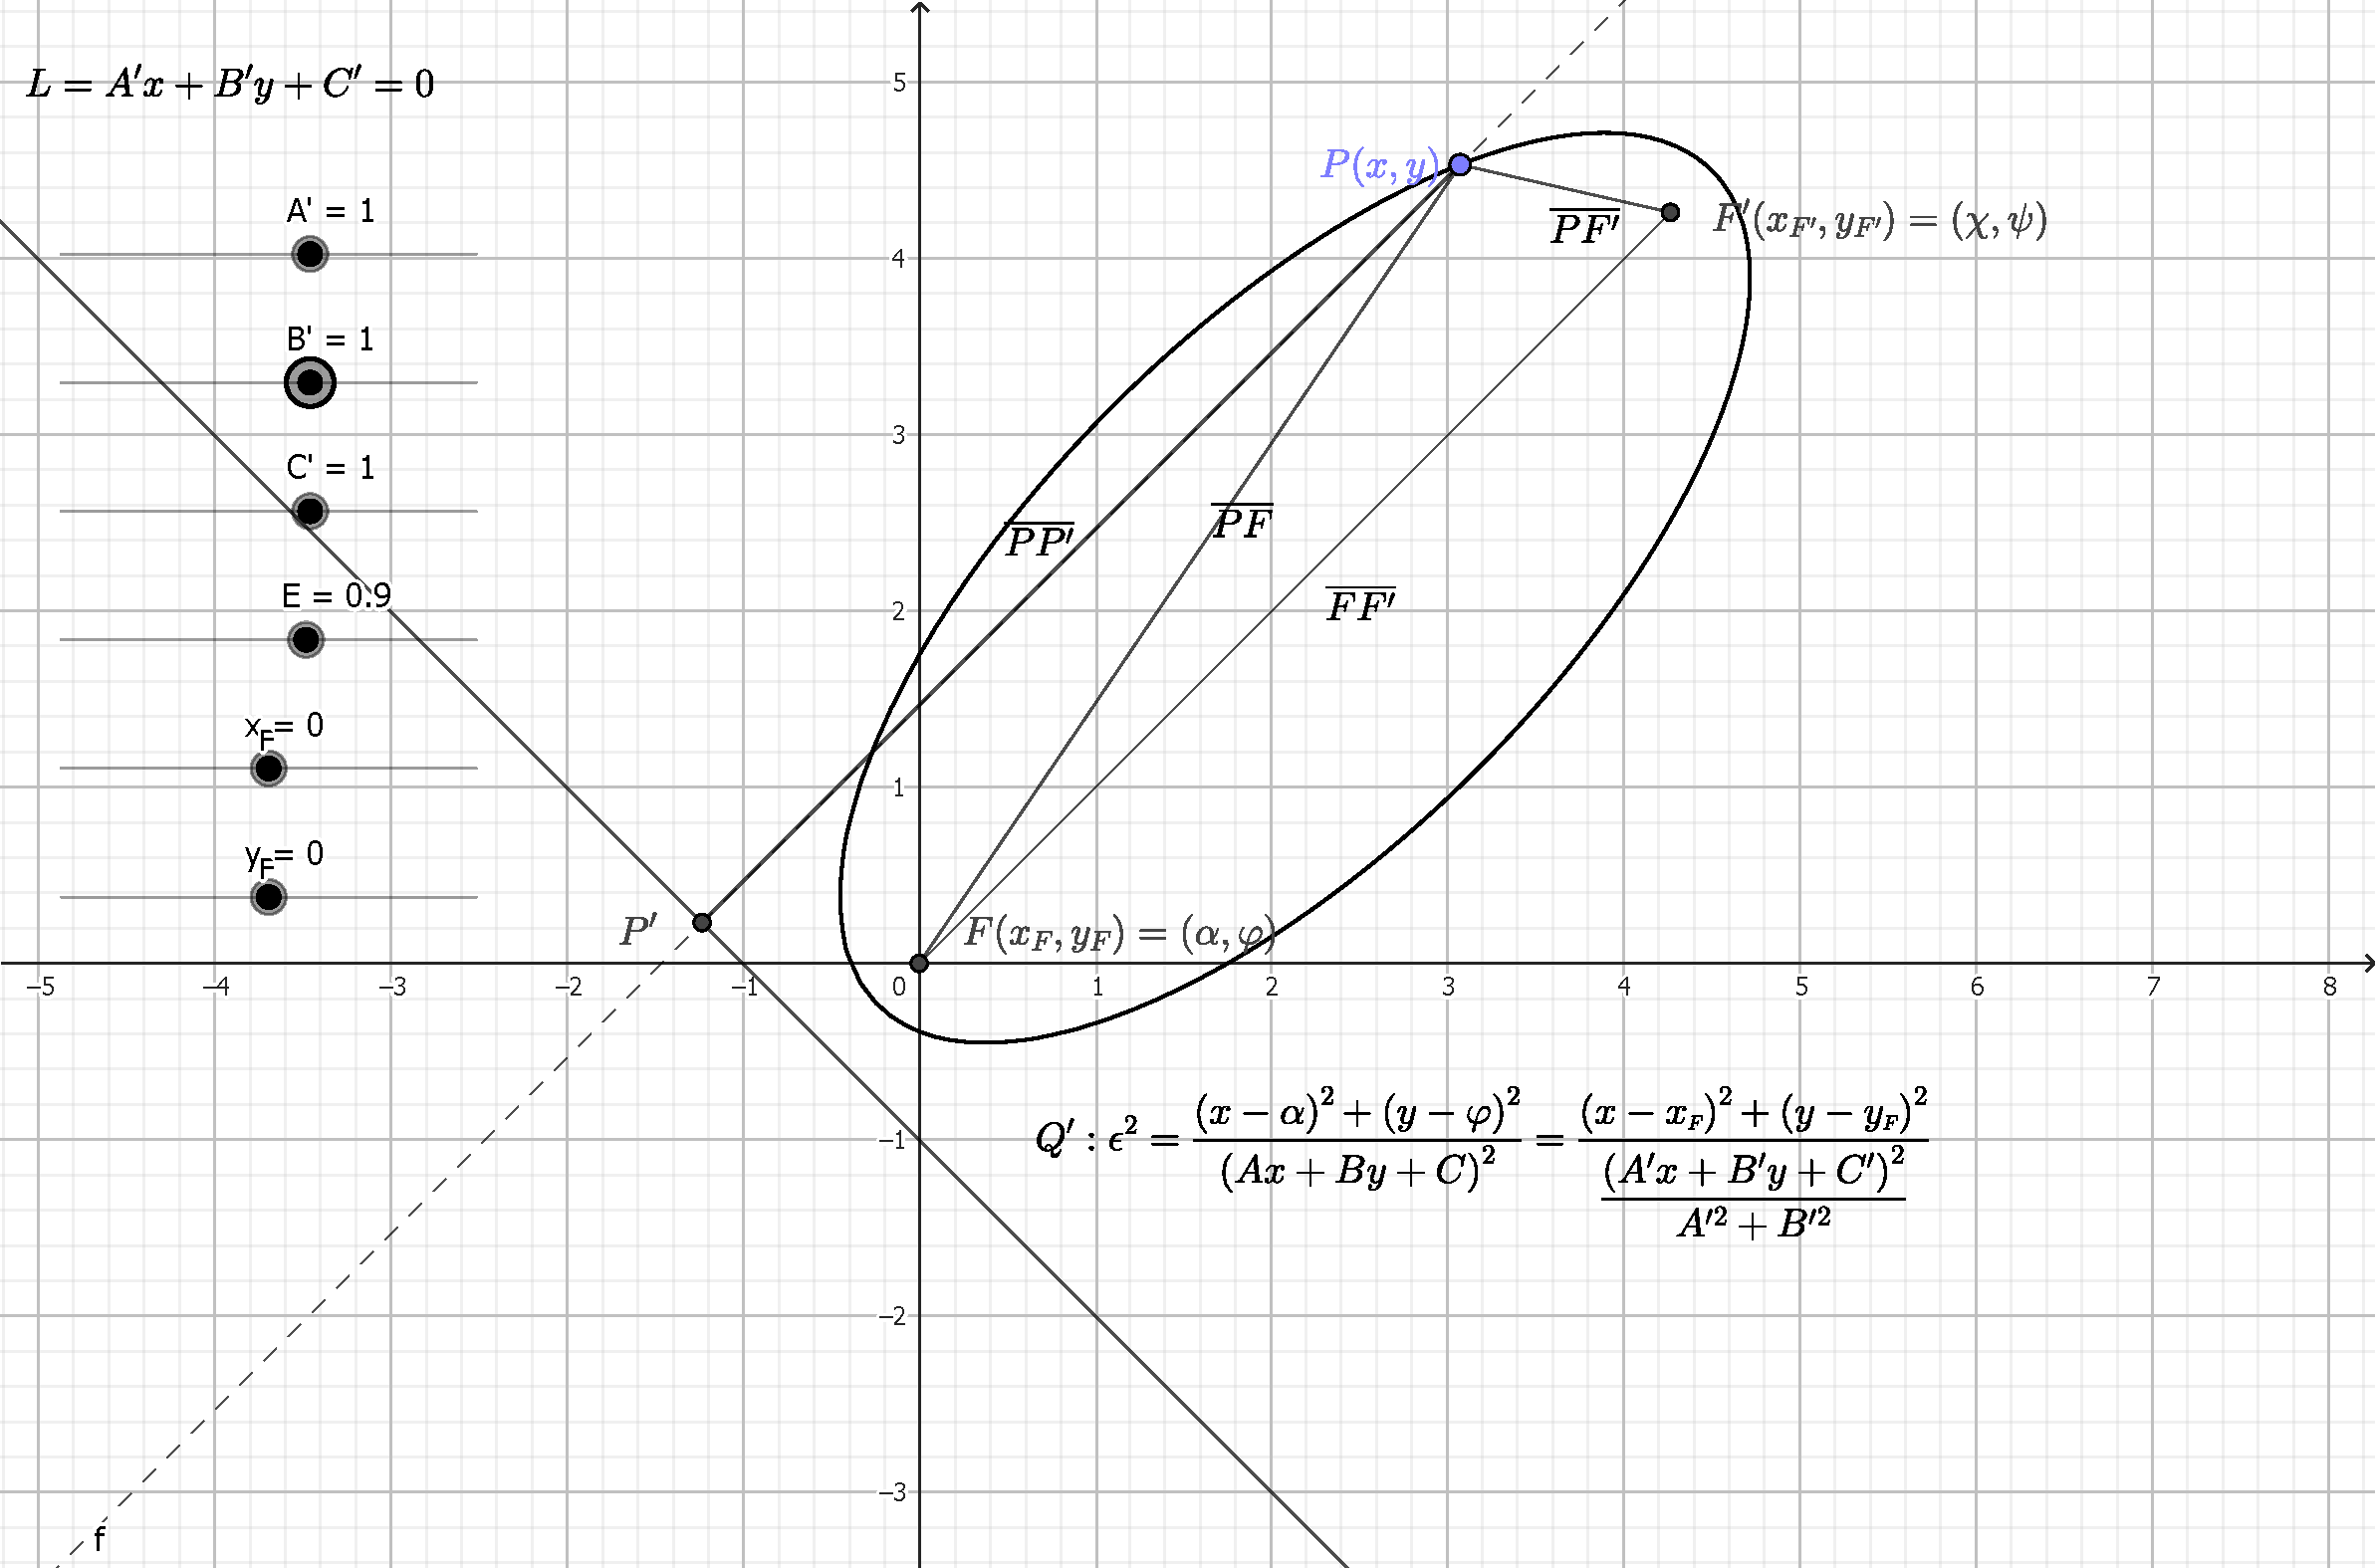
\includegraphics{img/conic-sections.pdf}

\begin{figure}
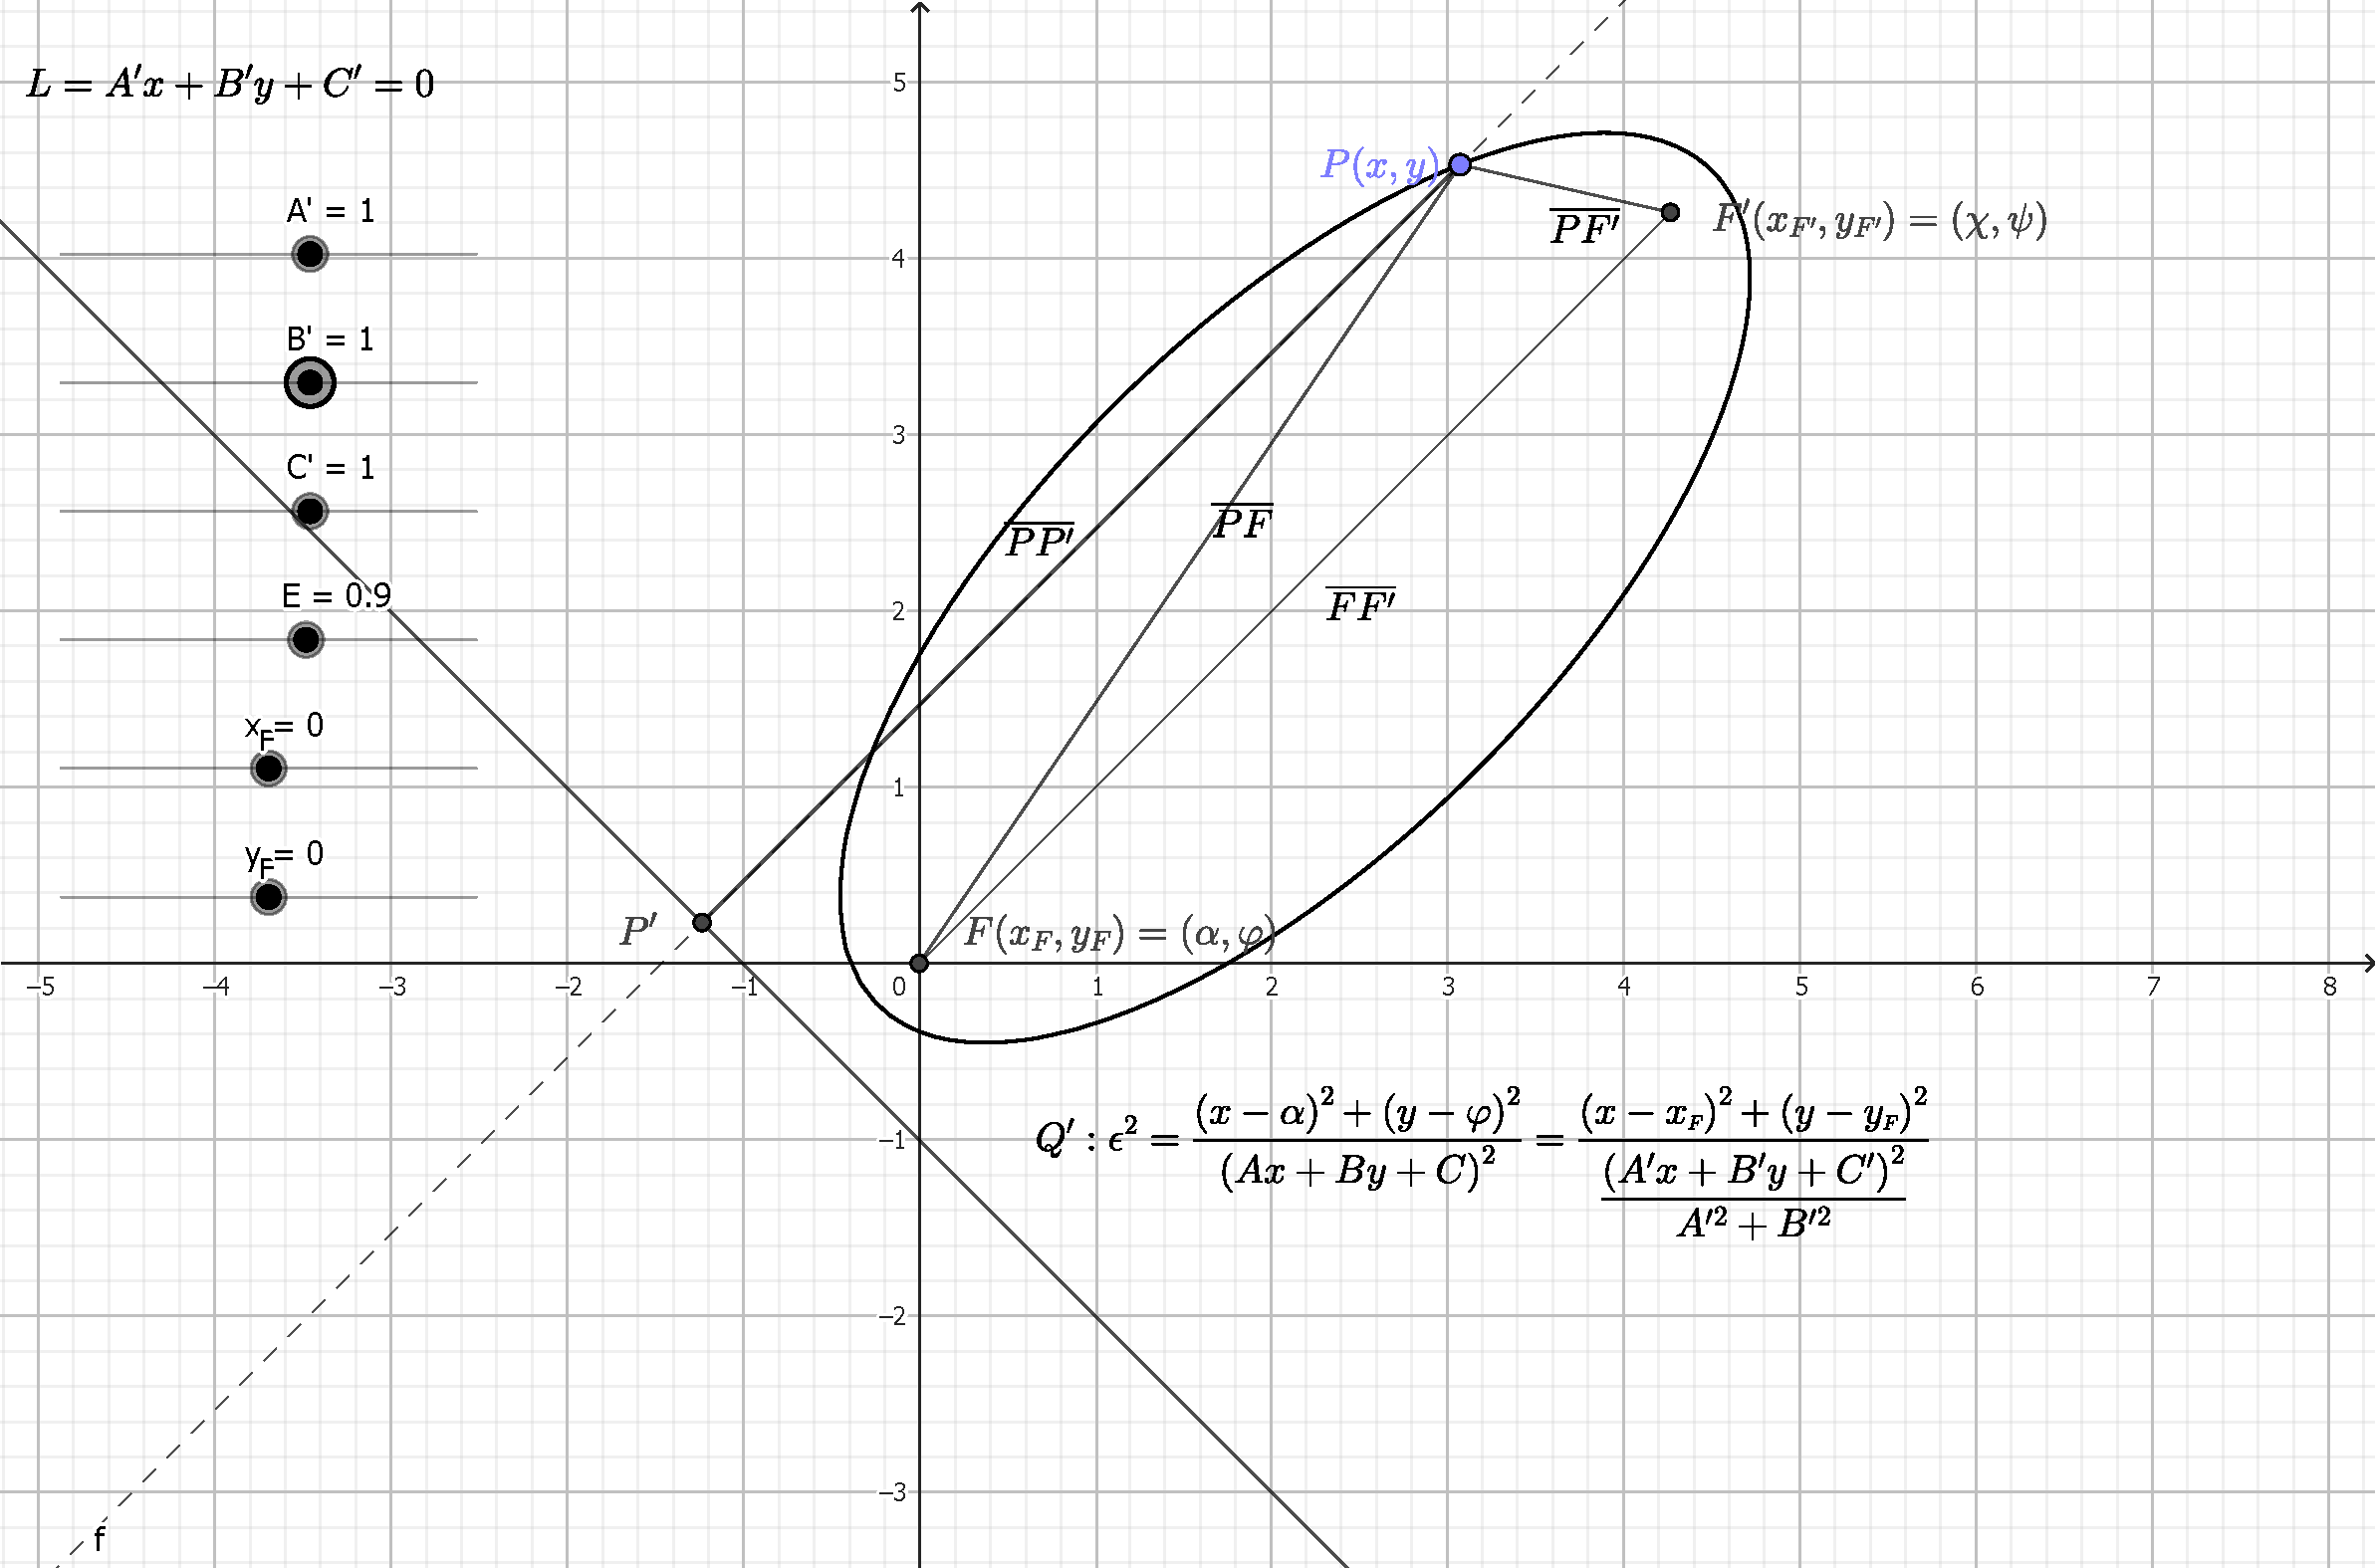
\includegraphics[width=0.75\linewidth]{img/conic-sections} \caption{conic sections}\label{fig:unnamed-chunk-26}
\end{figure}

\url{https://stackoverflow.com/questions/34064292/is-it-possible-to-include-svg-image-in-pdf-document-rendered-by-rmarkdown}

\subsection{horizontal rule}\label{horizontal-rule}

\begin{Shaded}
\begin{Highlighting}[]
\NormalTok{***}
\end{Highlighting}
\end{Shaded}

horizontal rule (or slide break)

\begin{center}\rule{0.5\linewidth}{0.5pt}\end{center}

\begin{Shaded}
\begin{Highlighting}[]
\FunctionTok{dim}\NormalTok{(iris) }
\end{Highlighting}
\end{Shaded}

\begin{verbatim}
## [1] 150   5
\end{verbatim}

\subsection{footnote}\label{footnote}

\subsection{hyperlink}\label{hyperlink}

PDF pandoc internal link will lose focus

\hyperref[equivalence-relation]{equivalence relation} {[}\ref{equivalence-relation}{]} \hyperref[equivalence-relation]{equivalence relation}\footnote{\{\ref{equivalence-relation}\} \hyperref[equivalence-relation]{equivalence relation}} \hyperref[equivalence-relation]{equivalence relation}\textsuperscript{{[}\ref{equivalence-relation}{]}}

\hyperref[equivalence-class]{equivalence class} {[}\ref{equivalence-class}{]} \hyperref[equivalence-class]{equivalence class}\footnote{\{\ref{equivalence-class}\} \hyperref[equivalence-class]{equivalence class}} \hyperref[equivalence-class]{equivalence class}\textsuperscript{{[}\ref{equivalence-class}{]}}

\hyperref[partition]{partition} {[}\ref{partition}{]} \hyperref[partition]{partition}\footnote{\{\ref{partition}\} \hyperref[partition]{partition}} \hyperref[partition]{partition}\textsuperscript{{[}\ref{partition}{]}}

\begin{itemize}
\tightlist
\item
  LaTeX

  \begin{itemize}
  \tightlist
  \item
    \hyperref[tikz]{TikZ}\textsuperscript{{[}\ref{tikz}{]}}

    \begin{itemize}
    \tightlist
    \item
      TikZ-3Dplot
    \item
      PGFplots
    \end{itemize}
  \item
    xypic = \hyperref[xy-pic]{xy-pic}\footnote{\{\ref{xy-pic}\} \hyperref[xy-pic]{xy-pic}}
  \end{itemize}
\item
  OverLeaf
\item
  MathCha
\item
  GeoGebra
\item
  Python

  \begin{itemize}
  \tightlist
  \item
    MatPlotLib
  \item
    Seaborn
  \item
    Plotly
  \end{itemize}
\end{itemize}

\subsection{code chunk}\label{code-chunk}

\subsubsection{code folding}\label{code-folding}

\url{https://cosname.github.io/rmarkdown-guide/rmarkdown-document.html\#html-code-folding}

\subsection{xaringan}\label{xaringan}

slide realtime preview with RStudio addin Infinite Moon Reader in RStudio viewer

\url{https://github.com/yihui/xaringan}

\url{https://www.youtube.com/watch?v=3n9nASHg9gc}

\subsection{embed a web page}\label{embed-a-web-page}

\subsubsection{iframe}\label{iframe}

\subsubsection{include URL}\label{include-url}

\url{https://bookdown.org/yihui/rmarkdown-cookbook/include-url.html}

\begin{verbatim}
knitr::include_url("https://yihui.org")
\end{verbatim}

\href{https://yihui.org}{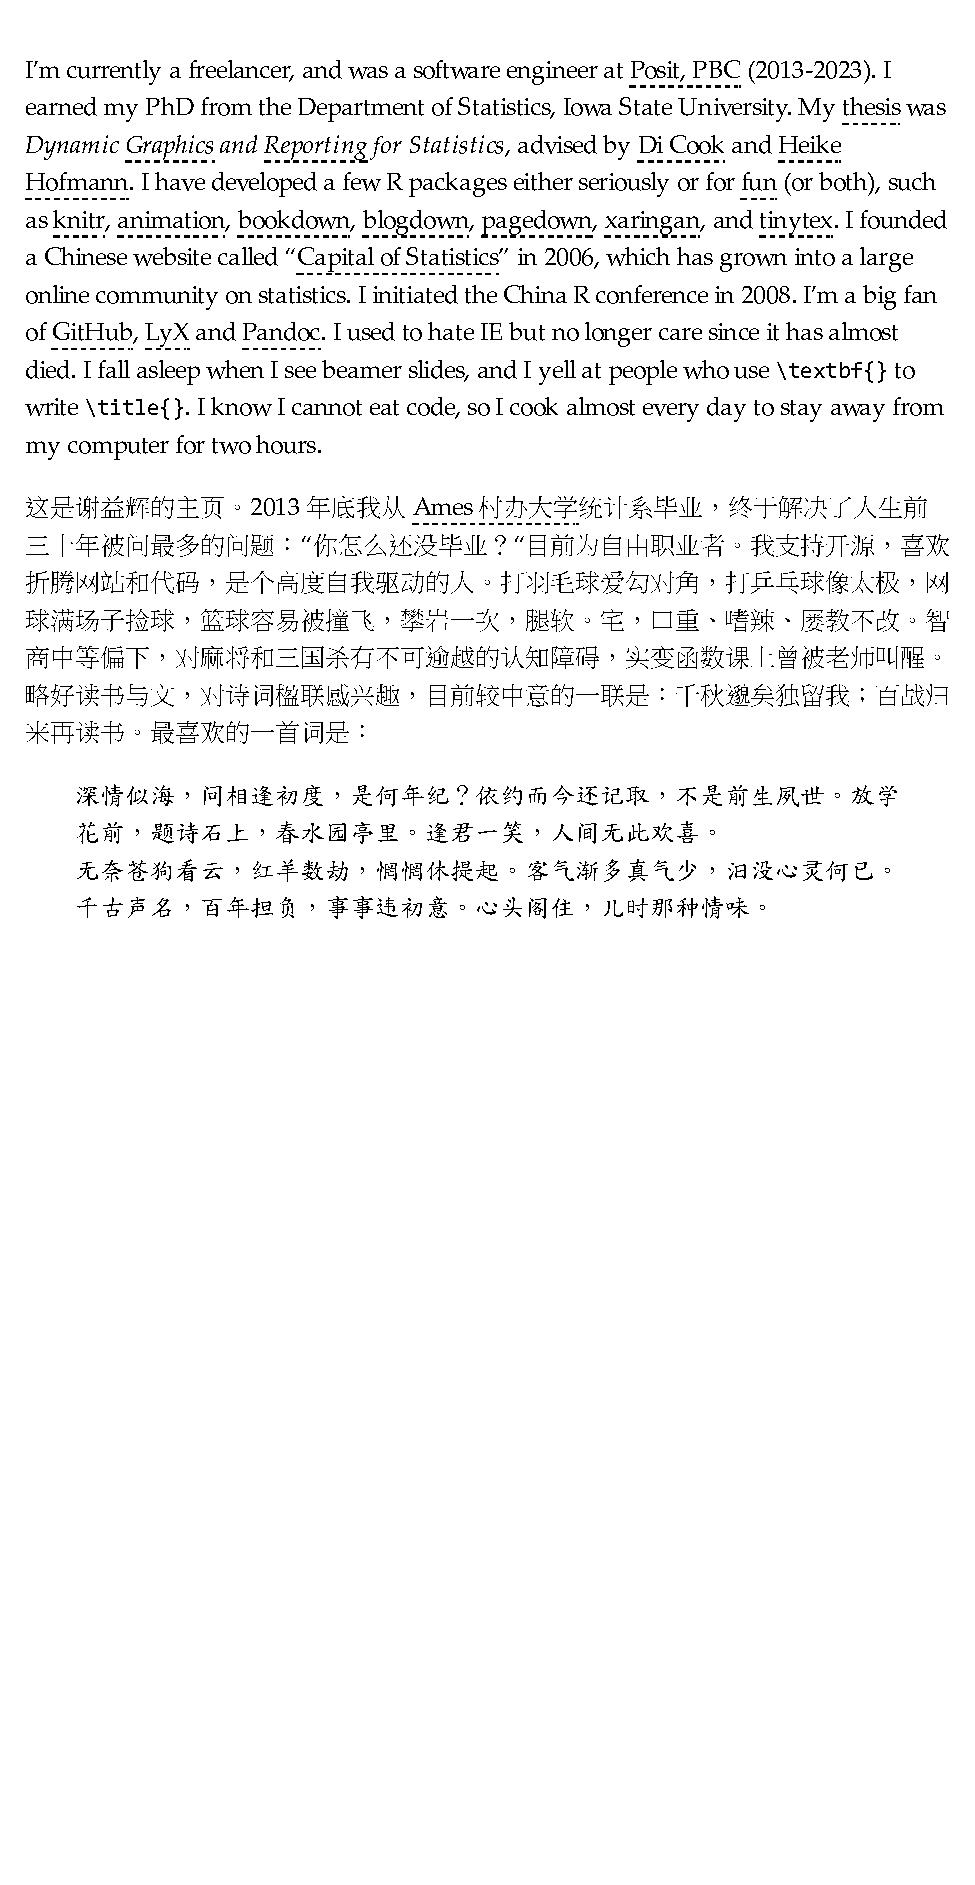
\includegraphics{202401280001-test_files/figure-latex/unnamed-chunk-30-1.pdf}}

\subsubsection{htmltools}\label{htmltools}

\url{https://stackoverflow.com/questions/36524238/include-html-files-in-r-markdown-file}

however \texttt{out.height} etc. not works

\section{Bookdown}\label{bookdown}

\subsection{system locale}\label{system-locale}

\url{https://bookdown.org/tpemartin/ntpu-programming-for-data-science/appendix-d-.html}

\begin{verbatim}
Sys.getlocale()
\end{verbatim}

Windows

\begin{verbatim}
Sys.setlocale(category = "LC_ALL", locale = "UTF-8")
\end{verbatim}

MacOS

\begin{verbatim}
Sys.setlocale(category = "LC_ALL", locale = "en_US.UTF-8")
\end{verbatim}

\url{https://bookdown.org/yihui/rmarkdown-cookbook/multi-column.html}

\subsection{\texorpdfstring{\texttt{render\_book()}}{render\_book()}}\label{render_book}

\url{https://bookdown.org/yihui/bookdown/build-the-book.html}

\begin{verbatim}
render_book(input = ".", output_format = NULL, ..., clean = TRUE,
  envir = parent.frame(), clean_envir = !interactive(),
  output_dir = NULL, new_session = NA, preview = FALSE,
  config_file = "_bookdown.yml")
\end{verbatim}

\subsection{\texorpdfstring{\texttt{serve\_book()}}{serve\_book()}}\label{serve_book}

\url{https://bookdown.org/yihui/bookdown/serve-the-book.html}

\begin{verbatim}
serve_book(dir = ".", output_dir = "_book", preview = TRUE,
  in_session = TRUE, quiet = FALSE, ...)
\end{verbatim}

\subsection{LaTeX}\label{latex-1}

\subsubsection{hyperlink, URL, href}\label{hyperlink-url-href}

\url{https://www.baeldung.com/cs/latex-hyperref-url-hyperlinks}

\begin{CJK}{UTF8}{bsmi}
https://www.omdte.com/小技巧讓-facebook和-line顯示中文網址,網址不再變亂碼/
\end{CJK}

\subsubsection{\texorpdfstring{ugly mathptmx \(\sum\)}{ugly mathptmx \textbackslash sum}}\label{ugly-mathptmx-sum}

PDF LaTeX \texttt{\textbackslash{}usepackage\{fdsymbol\}} to have \texttt{\textbackslash{}overrightharpoon} vector; however, there are too many side effects, including ugly mathptmx \(\sum\), \ldots{}

\begin{verbatim}

\usepackage{fdsymbol} % vector over accent, but will use mathptmx
% replace the rather ugly mathptmx \sum operator with the equivalent Computer Modern one
\let\sum\relax
\DeclareSymbolFont{CMlargesymbols}{OMX}{cmex}{m}{n}
\DeclareMathSymbol{\sum}{\mathop}{CMlargesymbols}{"50}
\end{verbatim}

\url{https://tex.stackexchange.com/questions/315102/different-sum-signs}

\url{https://tex.stackexchange.com/questions/275038/how-to-replace-mathptmx-sum-with-cm-sum}

\url{https://tex.stackexchange.com/questions/391410/calligraphic-symbols-are-too-fancy-with-mathptmx-package}

\url{https://blog.csdn.net/kongtaoxing/article/details/131005044}

In \texttt{preamble.tex}, add

\begin{verbatim}

% replace the rather ugly mathptmx \sum operator with the equivalent Computer Modern one
\let\sum\relax
\DeclareSymbolFont{CMlargesymbols}{OMX}{cmex}{m}{n}
\DeclareMathSymbol{\sum}{\mathop}{CMlargesymbols}{"50}

\DeclareMathAlphabet{\mathcal}{OMS}{cmsy}{m}{n}
\DeclareSymbolFont{largesymbols}{OMX}{cmex}{m}{n}
\end{verbatim}

\subsubsection{LaTeX package in HTML document}\label{latex-package-in-html-document}

\url{https://github.com/rstudio/rmarkdown/issues/1829}

\begin{verbatim}
---
title: "assignment"
author: "author"
output: html_document
---

$$
  \require{cancel}
  \cancel{x}
$$
\end{verbatim}

\[
  \cancel{x}
\]

\url{https://stackoverflow.com/questions/18189175/how-to-use-textup-with-mathjax}

\begin{quote}
\texttt{\textbackslash{}textup} is not available in MathJax. You can replace it with \texttt{\textbackslash{}mathrm}, \textbf{but \texttt{\textbackslash{}mathrm} does not interpret spaces}.
\end{quote}

\subsection{\texorpdfstring{depth of table of contents \texttt{toc\_depth}}{depth of table of contents toc\_depth}}\label{depth-of-table-of-contents-toc_depth}

\url{https://stackoverflow.com/questions/49009212/how-to-change-toc-depth-in-r-bookdown-gitbook}

\begin{Shaded}
\begin{Highlighting}[]
\AttributeTok{bookdown:}\FunctionTok{:gitbook}\KeywordTok{:}
\AttributeTok{    }\FunctionTok{toc\_depth}\KeywordTok{:}\AttributeTok{ }\DecValTok{2}
\end{Highlighting}
\end{Shaded}

\url{https://stackoverflow.com/questions/68537309/how-can-i-specific-the-initial-level-to-have-my-table-of-contents-be-expanded-to}

\begin{Shaded}
\begin{Highlighting}[]
\FunctionTok{toc}\KeywordTok{:}
\AttributeTok{  }\FunctionTok{collapse}\KeywordTok{:}\AttributeTok{ section}
\end{Highlighting}
\end{Shaded}

\subsection{multi-column layout / two columns}\label{multi-column}

\url{https://bookdown.org/yihui/rmarkdown-cookbook/multi-column.html}

\subsubsection{for both HTML and PDF}\label{for-both-html-and-pdf}

\hyperref[figure-size]{figure size}\textsuperscript{{[}\ref{figure-size}{]}}

\begin{quote}
Below is a Div containing three child Divs side by side. The Div in the middle is empty, just to add more space between the left and right Divs.
\end{quote}

\begin{verbatim}
:::::: {.cols data-latex=""}

::: {.col data-latex="{0.55\textwidth}"}
![](202401280001-test_files/figure-latex/unnamed-chunk-35-1.pdf)<!-- --> 
:::

::: {.col data-latex="{0.05\textwidth}"}
\ 
<!-- an empty Div (with a white space), serving as
a column separator -->
:::

::: {.col data-latex="{0.4\textwidth}"}
The figure on the left-hand side shows the `cars` data.

Lorem ipsum dolor sit amet, consectetur adipiscing elit, sed do
eiusmod tempor incididunt ut labore et dolore magna aliqua. Ut
enim ad minim veniam, quis nostrud exercitation ullamco laboris
nisi ut aliquip ex ea commodo consequat. Duis aute irure dolor
in reprehenderit in voluptate velit esse cillum dolore eu fugiat
nulla pariatur.
:::
::::::
\end{verbatim}

\texttt{\{r,\ echo=FALSE,\ fig.width=5,\ fig.height=4\}}

\begin{cols}

\begin{col}{0.55\textwidth}
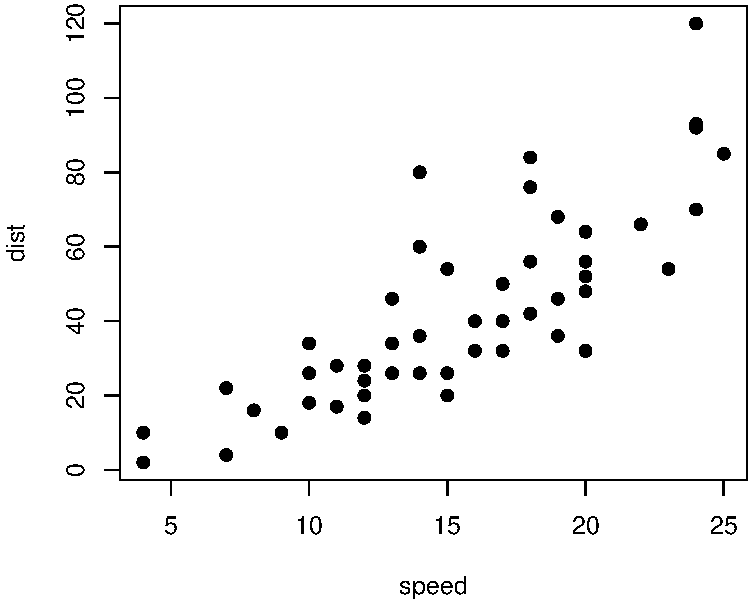
\includegraphics{202401280001-test_files/figure-latex/unnamed-chunk-36-1.pdf}

\end{col}

\begin{col}{0.05\textwidth}
~


\end{col}

\begin{col}{0.4\textwidth}
The figure on the left-hand side shows the \texttt{cars} data.

Lorem ipsum dolor sit amet, consectetur adipiscing elit, sed do
eiusmod tempor incididunt ut labore et dolore magna aliqua. Ut
enim ad minim veniam, quis nostrud exercitation ullamco laboris
nisi ut aliquip ex ea commodo consequat. Duis aute irure dolor
in reprehenderit in voluptate velit esse cillum dolore eu fugiat
nulla pariatur.

\end{col}

\end{cols}

\texttt{\{r,\ echo=FALSE,\ fig.width=10,\ fig.height=8,\ out.width\ =\ "100\%"\}}

\begin{cols}

\begin{col}{0.55\textwidth}
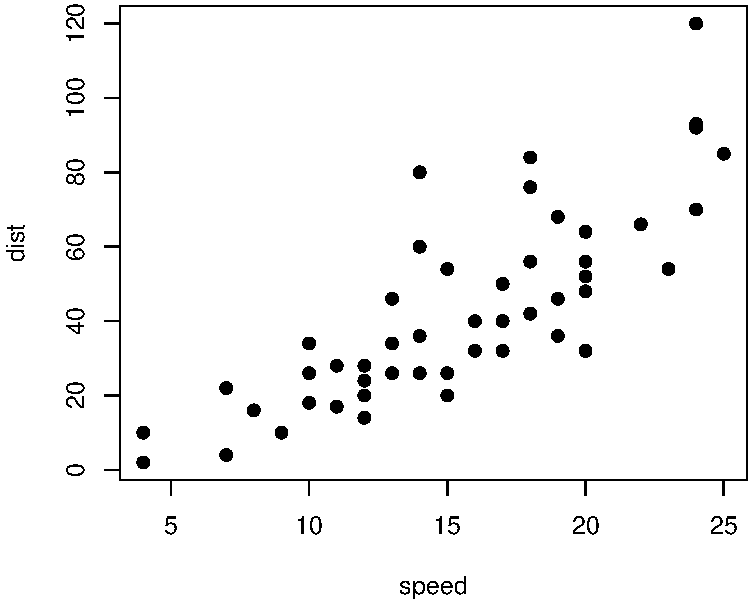
\includegraphics[width=1\linewidth]{202401280001-test_files/figure-latex/unnamed-chunk-37-1}

\end{col}

\begin{col}{0.05\textwidth}
~


\end{col}

\begin{col}{0.4\textwidth}
The figure on the left-hand side shows the \texttt{cars} data.

Lorem ipsum dolor sit amet, consectetur adipiscing elit, sed do
eiusmod tempor incididunt ut labore et dolore magna aliqua. Ut
enim ad minim veniam, quis nostrud exercitation ullamco laboris
nisi ut aliquip ex ea commodo consequat. Duis aute irure dolor
in reprehenderit in voluptate velit esse cillum dolore eu fugiat
nulla pariatur.

\end{col}

\end{cols}

\texttt{\{r,\ echo=FALSE,\ fig.width=10,\ fig.height=8\}}

\begin{cols}

\begin{col}{0.55\textwidth}
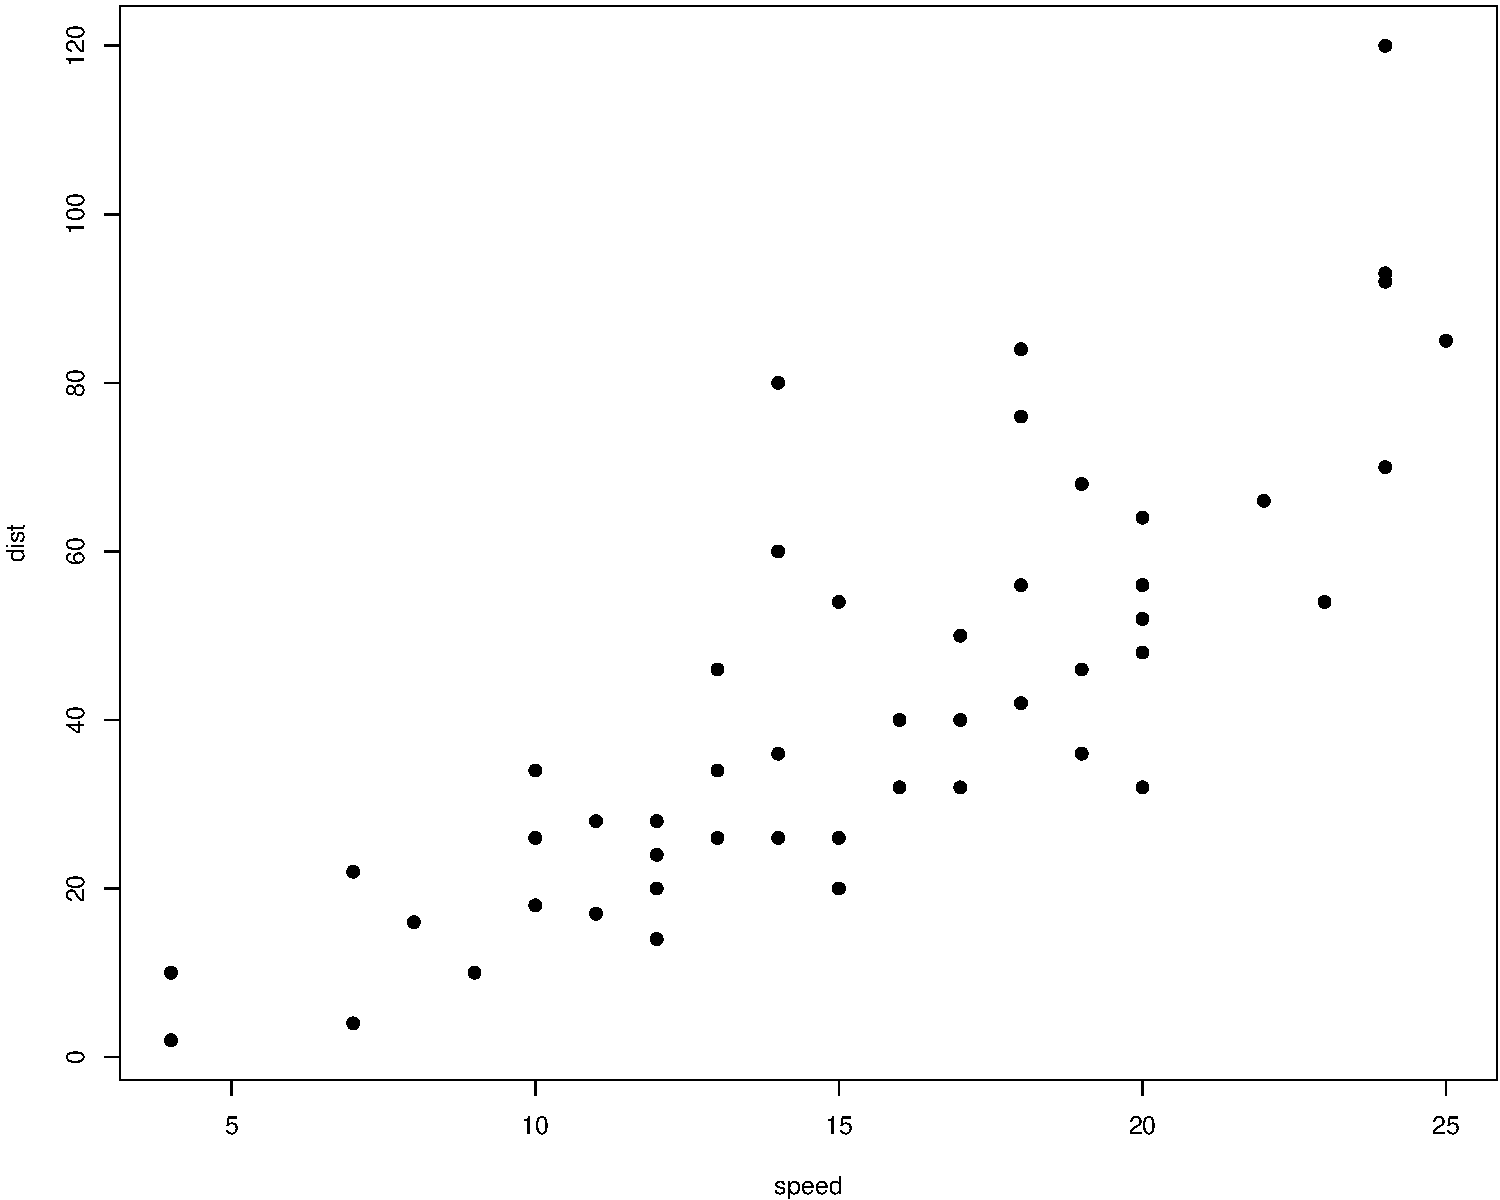
\includegraphics{202401280001-test_files/figure-latex/unnamed-chunk-38-1.pdf}

\end{col}

\begin{col}{0.05\textwidth}
~


\end{col}

\begin{col}{0.4\textwidth}
The figure on the left-hand side shows the \texttt{cars} data.

Lorem ipsum dolor sit amet, consectetur adipiscing elit, sed do
eiusmod tempor incididunt ut labore et dolore magna aliqua. Ut
enim ad minim veniam, quis nostrud exercitation ullamco laboris
nisi ut aliquip ex ea commodo consequat. Duis aute irure dolor
in reprehenderit in voluptate velit esse cillum dolore eu fugiat
nulla pariatur.

\end{col}

\end{cols}

\subsubsection{\texorpdfstring{multi-column \texttt{fig.cap} must use \texttt{fig.pos="H"}}{multi-column fig.cap must use fig.pos="H"}}\label{multi-column-fig.cap-must-use-fig.posh}

\url{https://community.rstudio.com/t/adding-fig-cap-caption-text-to-code-chunk-causes-figure-to-print-at-top-of-page-instead-of-where-it-should-be/30297}

\url{https://bookdown.org/yihui/rmarkdown-cookbook/figure-placement.html}

to avoid \texttt{LaTeX\ Error:\ Not\ in\ outer\ par\ mode} for caption in multi-column LaTeX PDF

in \texttt{output.yml} add \texttt{extra\_dependencies:\ {[}"float"{]}} under \texttt{bookdown::pdf\_book:}

include first chunk \texttt{knitr::opts\_chunk\$set(fig.pos\ =\ "H",\ out.extra\ =\ "")} in .Rmd

add \texttt{out.width=if\ (knitr:::is\_html\_output())\ \textquotesingle{}50\%\textquotesingle{}} for TikZ chunk

thus complete chunk beginning with \texttt{\{r,\ echo=FALSE,\ cache=TRUE,\ engine=\textquotesingle{}tikz\textquotesingle{},\ fig.ext=if\ (knitr:::is\_latex\_output())\ \textquotesingle{}pdf\textquotesingle{}\ else\ \textquotesingle{}png\textquotesingle{},\ fig.width=10,\ fig.height=2,\ out.width=if\ (knitr:::is\_html\_output())\ \textquotesingle{}100\%\textquotesingle{},\ fig.cap=\textquotesingle{}\textquotesingle{}\}}

\begin{cols}

\begin{col}{0.45\textwidth}

\begin{Shaded}
\begin{Highlighting}[]
\KeywordTok{\textbackslash{}begin}\NormalTok{\{}\ExtensionTok{tikzpicture}\NormalTok{\}}
  \FunctionTok{\textbackslash{}draw}\NormalTok{ ({-}1,1){-}{-}(0,0){-}{-}(1,2);}
\KeywordTok{\textbackslash{}end}\NormalTok{\{}\ExtensionTok{tikzpicture}\NormalTok{\}}
\end{Highlighting}
\end{Shaded}

\end{col}

\begin{col}{0.10\textwidth}
~

\end{col}

\begin{col}{0.45\textwidth}
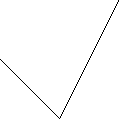
\includegraphics{202401280001-test_files/figure-latex/unnamed-chunk-40-1.pdf}

\end{col}

\end{cols}

LaTeX package \texttt{caption}

\url{https://tex.stackexchange.com/questions/128485/how-to-make-a-caption-via-captionof-and-extra-margins-adhere-to-minipage-marg}

What is the different between using \texttt{\textbackslash{}captionof\{table\}\{ABC\}} and \texttt{\textbackslash{}caption\{ABC\}}?

\url{https://tex.stackexchange.com/questions/514286/what-is-the-different-between-using-captionoftableabc-and-captionabc}

side-by-side table

\url{https://stackoverflow.com/questions/73745714/how-to-print-gt-tbl-tables-side-by-side-with-knitr-kable}

R ternary operator

\url{https://stackoverflow.com/questions/8790143/does-the-ternary-operator-exist-in-r}

\subsubsection{caption above figure}\label{caption-above-figure}

\url{https://stackoverflow.com/questions/56979022/caption-above-figure-in-html-rmarkdown}

\texttt{fig.topcaption=TRUE}

\subsubsection{for only HTML}\label{for-only-html}

\paragraph{CSS flex}\label{css-flex}

Here is the \textbf{first} Div.

\begin{Shaded}
\begin{Highlighting}[]
\FunctionTok{str}\NormalTok{(iris)}
\end{Highlighting}
\end{Shaded}

\begin{verbatim}
## 'data.frame':    150 obs. of  5 variables:
##  $ Sepal.Length: num  5.1 4.9 4.7 4.6 5 5.4 4.6 5 4.4 4.9 ...
##  $ Sepal.Width : num  3.5 3 3.2 3.1 3.6 3.9 3.4 3.4 2.9 3.1 ...
##  $ Petal.Length: num  1.4 1.4 1.3 1.5 1.4 1.7 1.4 1.5 1.4 1.5 ...
##  $ Petal.Width : num  0.2 0.2 0.2 0.2 0.2 0.4 0.3 0.2 0.2 0.1 ...
##  $ Species     : Factor w/ 3 levels "setosa","versicolor",..: 1 1 1 1 1 1 1 1 1 1 ...
\end{verbatim}

And this block will be put on the right:

\begin{Shaded}
\begin{Highlighting}[]
\FunctionTok{plot}\NormalTok{(iris[, }\SpecialCharTok{{-}}\DecValTok{5}\NormalTok{])}
\end{Highlighting}
\end{Shaded}

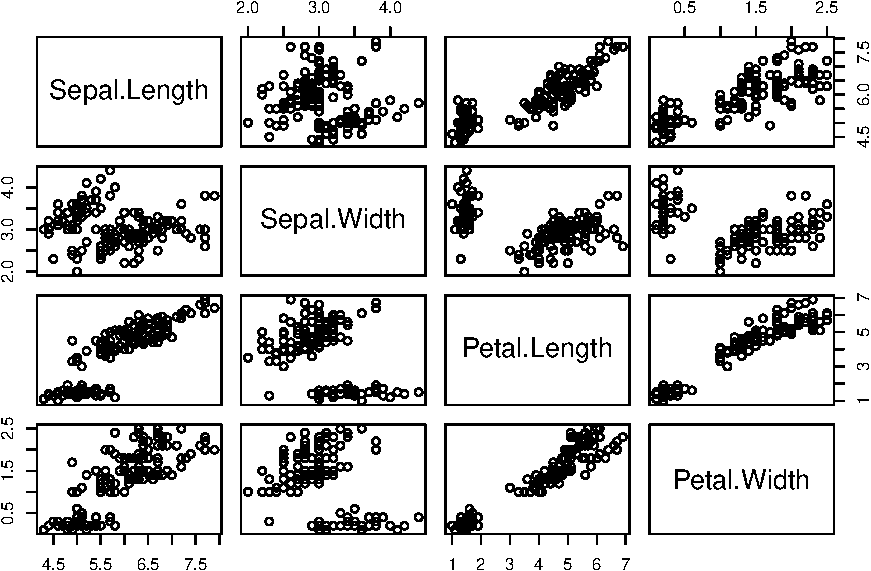
\includegraphics{202401280001-test_files/figure-latex/unnamed-chunk-42-1.pdf}

\paragraph{CSS grid}\label{css-grid}

\url{https://github.com/yihui/knitr/issues/1743}

\begin{CJK}{UTF8}{bsmi}
https://medium.com/enjoy-life-enjoy-coding/css-所以我說那個版能不能好切一點-grid-基本用法-cd763091cf70
\end{CJK}

\begin{Shaded}
\begin{Highlighting}[]
\FunctionTok{head}\NormalTok{(iris)}
\end{Highlighting}
\end{Shaded}

\begin{verbatim}
##   Sepal.Length Sepal.Width Petal.Length Petal.Width Species
## 1          5.1         3.5          1.4         0.2  setosa
## 2          4.9         3.0          1.4         0.2  setosa
## 3          4.7         3.2          1.3         0.2  setosa
## 4          4.6         3.1          1.5         0.2  setosa
## 5          5.0         3.6          1.4         0.2  setosa
## 6          5.4         3.9          1.7         0.4  setosa
\end{verbatim}

\begin{Shaded}
\begin{Highlighting}[]
\FunctionTok{plot}\NormalTok{(iris)}
\end{Highlighting}
\end{Shaded}

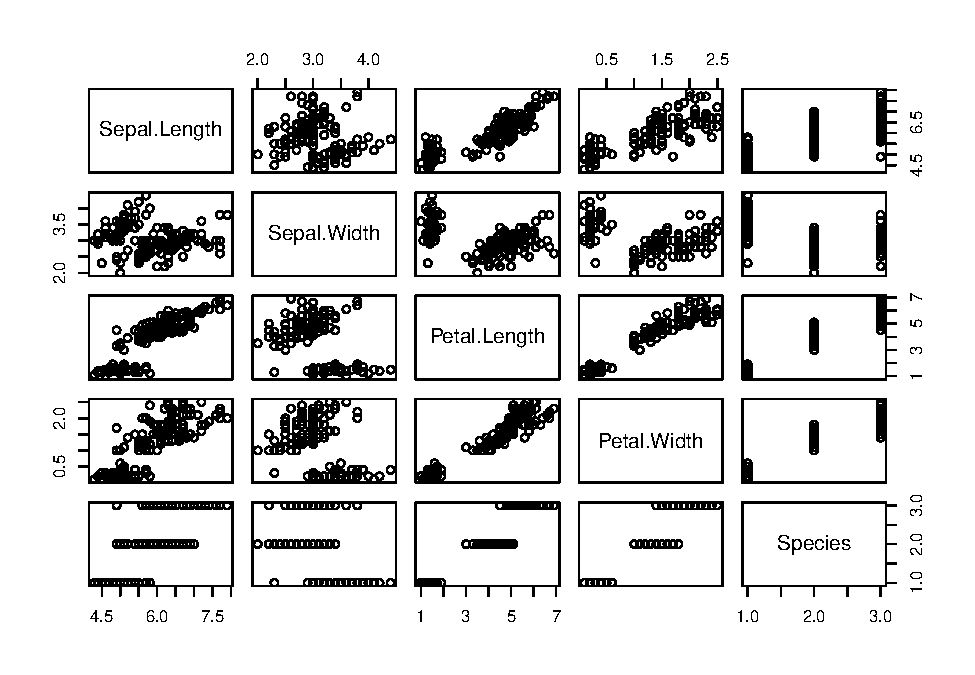
\includegraphics{202401280001-test_files/figure-latex/unnamed-chunk-44-1.pdf}

\section{conditional block/chunk for either HTML or PDF, and Chinese issue}\label{conditional-blockchunk-for-either-html-or-pdf-and-chinese-issue}

\url{https://stackoverflow.com/questions/76240244/bookdown-conditional-display-of-text-and-code-blocks-latex-pdf-vs-html}

\begin{CJK}{UTF8}{bsmi}等價關係 equivalence relation \label{def:equivalence-relation}
\end{CJK}
\begin{CJK}{UTF8}{bsmi}
\begin{align*}
 & R\text{ is an equivalence relation over }A\times B\\
\Leftrightarrow & \begin{cases}
R=\sim=\left\{ \left\langle x,y\right\rangle \middle|x\sim y\right\} \subseteq A\times B & \left(\text{e}\right)\text{equivalence 等價}\\
\vdots & \vdots
\end{cases}\\
\Leftrightarrow & \begin{cases}
R=\left\{ \left\langle x,y\right\rangle \middle|xRy\right\} \subseteq A\times B & \left(R\right)\text{relation}\\
\forall\left\langle x,y\right\rangle \in R\left(xRx\right) & \left(r\right)\text{reflexive}\\
\forall\left\langle x,y\right\rangle \in R\left(xRy\Rightarrow yRx\right) & \left(s\right)\text{symmetric}\\
\forall\left\langle x,y\right\rangle ,\left\langle y,z\right\rangle \in R\left(\begin{cases}
xRy\\
yRz
\end{cases}\Rightarrow xRz\right) & \left(t\right)\text{transitive}
\end{cases}\Leftrightarrow\begin{cases}
R=\left\{ \left\langle x,y\right\rangle \middle|xRy\right\} \subseteq A\times B & \text{關係}\\
\forall\left\langle x,y\right\rangle \in R\left(\left\langle x,x\right\rangle \in R\right) & \text{自反}\\
\forall\left\langle x,y\right\rangle \in R\left(\left\langle y,x\right\rangle \in R\right) & \text{對稱}\\
\forall\left\langle x,y\right\rangle ,\left\langle y,z\right\rangle \in R\left(\left\langle x,z\right\rangle \in R\right) & \text{遞移}
\end{cases}
\end{align*}
\end{CJK}

\section{video embedding}\label{video-embedding}

\url{https://stackoverflow.com/questions/42543206/r-markdown-compile-error}

always\_allow\_html: true

\begin{Shaded}
\begin{Highlighting}[]
\FunctionTok{install.packages}\NormalTok{(}\StringTok{"webshot"}\NormalTok{)}
\NormalTok{webshot}\SpecialCharTok{::}\FunctionTok{install\_phantomjs}\NormalTok{()}
\end{Highlighting}
\end{Shaded}

however webshot not work

Error: cannot find bilibili.com

\url{https://cran.r-project.org/web/packages/vembedr/vignettes/embed.html}

\begin{verbatim}
## embed_youtube("0LFg5dvPOoc")
\end{verbatim}

\subsection{timestamp}\label{timestamp}

\begin{itemize}
\tightlist
\item
  YouTube: \url{https://www.youtube.com/embed/\%7BvideoID\%7D?start=\%7Bsecond\%7D}
\item
  BiliBili: \url{https://player.bilibili.com/player.html?bvid=\%7BvideoID\%7D&autoplay=0&t=\%7Bsecond\%7D}
\end{itemize}

\section{equation term coloring}\label{equation-term-coloring}

\hyperref[latex-annotation-by-tikz]{LaTeX annotation by TikZ}\textsuperscript{{[}\ref{latex-annotation-by-tikz}{]}}

\subsection{font color}\label{font-color}

RegEx replacement in RStudio for \texttt{\{\textbackslash{}\textbackslash{}color\{(\textbackslash{}w+)\}} in LyX to be replaced with \texttt{\textbackslash{}\textbackslash{}color\{\$1\}\{} in HTML document, and remain the same for PDF document

In HTML document, if no \texttt{\{\}} for text range, only the first following term will take effect

\texttt{\textbackslash{}color\{orange\}x=y}

\[\color{orange}x=y\]
\texttt{\textbackslash{}color\{orange\}} and \texttt{\textbackslash{}color\{cyan\}} are better color for HTML GitBook \texttt{White} and \texttt{Night} themes and PDF

\texttt{\textbackslash{}color\{cyan\}\{x=y\}}

\[\color{orange}{x=y}\]

\texttt{\textbackslash{}color\{cyan\}\{x=y\}}

\[\color{cyan}{x=y}\]

\begin{Shaded}
\begin{Highlighting}[]
\NormalTok{::: \{show{-}in="html"\}}

\NormalTok{$$}
\NormalTok{\textbackslash{}dfrac\{\textbackslash{}colorbox\{\#FFD1DC\}\{$\textbackslash{}epsilon\^{}\{2\}\textbackslash{}left(y\_\{\{\textbackslash{}scriptscriptstyle F\}\}{-}y\_\{\{\textbackslash{}scriptscriptstyle L\}\}\textbackslash{}right)\^{}\{2\}$\}\}\{1{-}\textbackslash{}epsilon\^{}\{2\}\}}
\NormalTok{$$}

\NormalTok{:::}

\NormalTok{::: \{show{-}in="pdf"\}}

\NormalTok{$$}
\NormalTok{\textbackslash{}dfrac\{\textbackslash{}colorbox\{red!50\}\{\textbackslash{}text\{\textbackslash{}ensuremath\{\textbackslash{}epsilon\^{}\{2\}\textbackslash{}left(y\_\{\{\textbackslash{}scriptscriptstyle F\}\}{-}y\_\{\{\textbackslash{}scriptscriptstyle L\}\}\textbackslash{}right)\^{}\{2\}\}\}\}\}\{1{-}\textbackslash{}epsilon\^{}\{2\}\}}
\NormalTok{$$}

\NormalTok{:::}
\end{Highlighting}
\end{Shaded}

\subsection{background color}\label{background-color}

\url{https://bookdown.org/yihui/rmarkdown-cookbook/font-color.html}

LaTex color

\url{https://latexcolor.com/}

\url{https://www.overleaf.com/learn/latex/Using_colors_in_LaTeX}

\url{https://latex-tutorial.com/color-latex/\#}:\textasciitilde:text=To\%20summarize\%2C\%20pyellow!50efined\%20colors\%20in,when\%20loading\%20the\%20xcolor\%20package.

LaTex color methods

color frame

\url{https://tex.stackexchange.com/questions/582748/highlight-equation-with-boxes-and-arrows}

color box

\url{https://tex.stackexchange.com/questions/567739/how-to-move-and-size-colorbox}

color box with round corners

\url{https://tex.stackexchange.com/questions/568880/color-box-with-rounded-corners}

highlighting

\url{https://tex.stackexchange.com/questions/318991/highlighting-math}

\url{https://forum.remnote.io/t/highlighting-latex-formulas/149}

LyX

\url{https://tex.stackexchange.com/questions/250069/create-a-color-box}
\url{https://latexlyx.blogspot.com/2013/12/lyx.html}

\url{https://tex.stackexchange.com/questions/635486/prevent-lyx-from-escaping-math-in-color-box-title}

Bookdown - conditional display of text and code blocks (LaTeX/PDF vs.~HTML)
\url{https://stackoverflow.com/questions/76240244/bookdown-conditional-display-of-text-and-code-blocks-latex-pdf-vs-html}

\begin{align*}
\colorbox{yellow!50}{$F$}= & \colorbox{yellow!50}{$ma$}\\
\end{align*}

\url{https://community.rstudio.com/t/highlighting-text-inline-in-rmarkdown-or-bookdown-pdf/35118/4}
\definecolor{hightlightColor}{HTML}{FFFF66}

\begin{align*}
\colorbox{hightlightColor}{$F$}= & \colorbox{yellow!50}{$ma$}\\
\end{align*}

\begin{align*}
\colorbox{hightlightColor}{\ensuremath{F}}= & \colorbox{yellow!50}{\ensuremath{F}}\\
\end{align*}

\begin{equation}
\colorbox{yellow!50}{$F$}=\colorbox{yellow!50}{$ma$}
\end{equation}

\[
\colorbox{hightlightColor}{$F$}=\colorbox{yellow!50}{$ma$}
\]

\[
\colorbox{yellow!50}{$Y = \beta_0 + \beta_1 X_1 + \ldots + \beta_n X_n$}
\]

\section{link and reference}\label{link-and-reference}

\url{https://stackoverflow.com/questions/57469501/cross-referencing-bookdownhtml-document2-not-working}

\begin{equation}
  E=mc^2
  \label{eq:emc}
\end{equation}

\texttt{\textbackslash{}@ref(nice-label)} \ref{nice-label}

\texttt{{[}link\ to\ partition{]}{[}partition{]}} \hyperref[partition]{link to partition}

\texttt{{[}partition{]}} \texttt{\textbackslash{}@ref(partition)}

\hyperref[partition]{partition} {[}\#partition{]} (\ref{partition}) @ref(\#partition)

\texttt{{[}equivalence\ class{]}} \texttt{\textbackslash{}@ref(equivalence-class)}

\hyperref[equivalence-class]{equivalence class} (\ref{equivalence-class})

\hyperref[equivalence-class]{equivalence class} {[}\#equivalence class{]} (@ref(equivalence class)) @ref(\#equivalence class)

{[}equivalence-class{]} {[}\#equivalence-class{]} (\ref{equivalence-class}) @ref(\#equivalence-class)

X {[}equivalence-class.html{]} {[}equivalence-class.html\#equivalence-class{]} (@ref(equivalence-class.html)) @ref(equivalence-class.html\#equivalence-class)

\hyperref[equivalence-relation]{equivalence relation} {[}\#equivalence relation{]} (@ref(equivalence relation)) @ref(\#equivalence relation)

{[}equivalence-relation{]} {[}\#equivalence-relation{]} (\ref{equivalence-relation}) @ref(\#equivalence-relation)

X {[}equivalence-relation.html{]} {[}equivalence-relation.html\#equivalence-relation{]} (@ref(equivalence-relation.html)) @ref(equivalence-relation.html\#equivalence-relation)

\section{number and reference equations}\label{nice-label}

\url{https://stackoverflow.com/questions/71595882/rstudio-error-in-windows-running-pdflatex-exe-on-file-name-tex-exit-code-10}

\url{https://bookdown.org/yihui/rmarkdown/bookdown-markdown.html\#equations}

\texttt{\textbackslash{}\#eq:emc}
\texttt{\textbackslash{}@ref(eq:emc)}

\url{https://stackoverflow.com/questions/55923290/consistent-math-equation-numbering-in-bookdown-across-pdf-docx-html-output}

\begin{equation}
\begin{aligned}
 & C\text{ is an equivalence class of }a\text{ on }A\\
\Leftrightarrow & \left[a\right]_{\sim}=C=\left\{ x\middle|\begin{cases}
a\in A\\
x\in A\\
x\sim a\\
\sim\text{ is an equivalence relation over }A\times A=A^{2}
\end{cases}\right\} \subseteq A\ne\emptyset\\
\Leftrightarrow & \left[a\right]=\left[a\right]_{\sim}=\left\{ x\middle|\begin{cases}
a\in A\\
x\in A\\
x\sim a\\
\sim\text{ is an equivalence relation on }A
\end{cases}\right\} \subseteq A\ne\emptyset\\
\Rightarrow & \left[a\right]_{\sim}=\left\{ x\middle|x\sim a\right\} \subseteq A\ne\emptyset
\end{aligned}
\label{eq:eqclass}
\end{equation}

\url{https://bookdown.org/yihui/rmarkdown/bookdown-markdown.html\#cross-referencing}

This cross reference is the Fig. \ref{fig:parabola-arc-with-points}

\url{https://stackoverflow.com/questions/51595939/bookdown-cross-reference-figure-in-another-file}

I ran into the same issue and came up with this solution if you aim at compiling 2 different pdfs. It relies on LaTeX's xr package for cross references: \url{https://stackoverflow.com/a/52532269/576684}

\section{footnote}\label{footnote-1}

\begin{Shaded}
\begin{Highlighting}[]
\NormalTok{noun\^{}}\CommentTok{[}\OtherTok{This is a footnote}\CommentTok{]}

\NormalTok{noun}\OtherTok{[\^{}202401260000{-}test{-}cross{-}link{-}1]}

\OtherTok{[\^{}202401260000{-}test{-}cross{-}link{-}1]: }\NormalTok{This is a footnote.}
\end{Highlighting}
\end{Shaded}

noun\footnote{This is a footnote.}

\section{citation}\label{citation}

\url{https://stackoverflow.com/questions/48965247/use-csl-file-for-pdf-output-in-bookdown/49145699\#49145699}

citation 1\textsuperscript{\citeproc{ref-noauthor_bookdown_2019}{3}} citation 2\textsuperscript{\citeproc{ref-noauthor_bookdown_2019}{3}}

citation 3\textsuperscript{\citeproc{ref-ccjou2009}{4}} citation 4\textsuperscript{\citeproc{ref-ccjou2009}{4}}

\subsection{\texorpdfstring{citation in \texttt{fig.cap}}{citation in fig.cap}}\label{citation-in-fig.cap}

\url{https://tex.stackexchange.com/questions/591882/citation-within-a-latex-figure-caption-in-rmarkdown}

\texttt{(ref:rudolph)\ *nice*\ cite:\ {[}@Lam94{]}.}

\texttt{(ref:campbell1963)\ *nice*\ cite:\ {[}@campbell1963{]}.}

\texttt{(ref:campbell1963)\ ({[}@campbell1963{]}}

\texttt{(ref:campbell1963)\ \textbackslash{}\ {[}@campbell1963{]}}



\begin{figure}
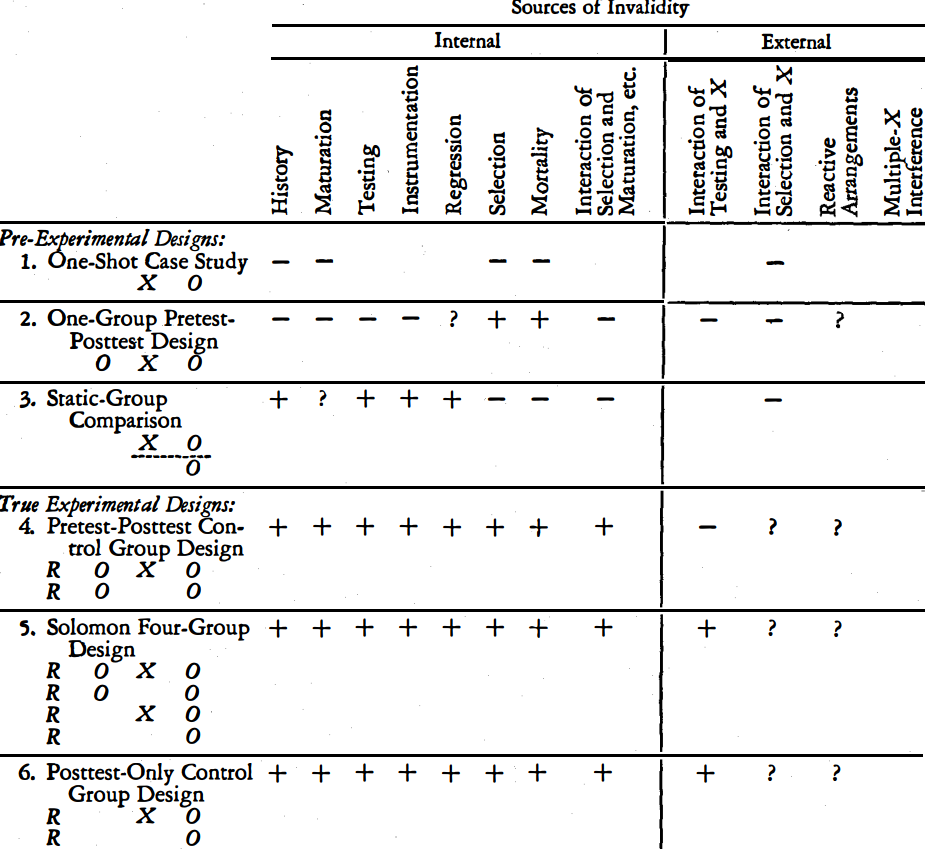
\includegraphics[width=0.65\linewidth]{img/pre-and-true-experimental-designs} \caption{pre- and true experimental designs (~\textsuperscript{\citeproc{ref-campbell1963}{5}} p.8)}\label{fig:unnamed-chunk-55}
\end{figure}

\subsection{backreference}\label{backreference}

\url{https://community.rstudio.com/t/how-to-create-a-backreference-to-place-of-citation-in-rmarkdown/84866}

\url{https://blog.csdn.net/RobertChenGuangzhi/article/details/50455429}

\url{https://latex.org/forum/viewtopic.php?t=3722}

\section{environment for definition, theorem, proof}\label{environment-for-definition-theorem-proof}

\url{https://bookdown.org/yihui/rmarkdown/bookdown-markdown.html}

\url{https://github.com/rstudio/rstudio/issues/5264}

\texttt{@howthebodyworks} Ideally, previews of such equations should also work inside a theorem, although I could survive without that.

\url{https://github.com/rstudio/rstudio/issues/8773}

\begin{theorem}[Theorem Name]
\protect\hypertarget{thm:label}{}\label{thm:label}Here is my theorem.
\end{theorem}

\begin{proof}[Proof Name]
Here is my proof.
\end{proof}

\begin{theorem}[Pythagorean theorem]
\protect\hypertarget{thm:pyth}{}\label{thm:pyth}For a right triangle, if \(c\) denotes the length of the hypotenuse
and \(a\) and \(b\) denote the lengths of the other two sides, we have

\[a^2 + \color{cyan}b^2 \overset{\ref{eq:emc}}= \color{red}{c^2} \]
\end{theorem}

\begin{definition}[Definition Name]
\protect\hypertarget{def:unnamed-chunk-57}{}\label{def:unnamed-chunk-57}Here is my definition.
\end{definition}

\hyperref[nice-label]{number and reference equations}

\eqref{eq:eqclass}

\eqref{eq:emc}

\ref{thm:pyth}

\begin{figure}
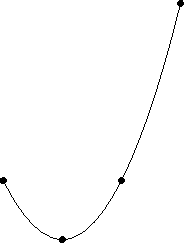
\includegraphics[width=0.25\linewidth]{202401280001-test_files/figure-latex/parabola-arc-with-points-1} \caption{parabola arc with points}\label{fig:parabola-arc-with-points}
\end{figure}

\section{slide or presentation}\label{slide-or-presentation}

\subsection{Xaringan and Infinite Moon Reader}\label{xaringan-and-infinite-moon-reader}

\url{https://rpubs.com/RW1304/xarigan-zh}

\url{https://slides.yihui.org/xaringan/\#1}

\url{https://slides.yihui.org/xaringan/zh-CN.html\#1}

\url{https://github.com/yihui/xaringan/tree/master}

\url{https://bookdown.org/yihui/rmarkdown/xaringan.html}

\subsection{ioslides}\label{ioslides}

\url{https://www.youtube.com/watch?v=gkyjTcpCITM}

\url{https://bookdown.org/yihui/rmarkdown/ioslides-presentation.html}

\url{https://stackoverflow.com/questions/63749683/how-to-set-up-theorem-environment-in-the-rmarkdown-presentation}

\begin{Shaded}
\begin{Highlighting}[]
\PreprocessorTok{{-}{-}{-}}
\FunctionTok{title}\KeywordTok{:}\AttributeTok{ }\StringTok{"Theorem demo"}
\FunctionTok{output}\KeywordTok{:}
\AttributeTok{  }\FunctionTok{ioslides\_presentation}\KeywordTok{:}
\AttributeTok{    }\FunctionTok{css}\KeywordTok{:}\AttributeTok{ style.css}
\PreprocessorTok{{-}{-}{-}}
\end{Highlighting}
\end{Shaded}

\begin{Shaded}
\begin{Highlighting}[]

\CommentTok{/* theorem environment \_ plain */}

\CommentTok{/*}
\CommentTok{.theorem \{}
\CommentTok{  display: block;}
\CommentTok{  font{-}style: italic;}
\CommentTok{  font{-}size: 24px;}
\CommentTok{  font{-}family: "Times New Roman";}
\CommentTok{  color: black;}
\CommentTok{\}}
\CommentTok{.theorem::before \{}
\CommentTok{  content: "Theorem. ";}
\CommentTok{  font{-}weight: bold;}
\CommentTok{  font{-}style: normal;}
\CommentTok{\}}
\CommentTok{.theorem[text]::before \{}
\CommentTok{  content: "Theorem (" attr(text) ") ";}
\CommentTok{\}}
\CommentTok{.theorem p \{}
\CommentTok{  display: inline;}
\CommentTok{\}}
\CommentTok{*/}

\CommentTok{/* theorem environment \_ Copenhagen style */}

\CommentTok{/*}
\CommentTok{.theorem \{}
\CommentTok{  display: block;}
\CommentTok{  font{-}style: italic;}
\CommentTok{  font{-}size: 24px;}
\CommentTok{  font{-}family: "Times New Roman";}
\CommentTok{  color: black;}
\CommentTok{  border{-}radius: 10px;}
\CommentTok{  background{-}color: rgb(222,222,231);}
\CommentTok{  box{-}shadow: 5px 10px 8px \#888888;}
\CommentTok{\}}
\CommentTok{.theorem::before \{}
\CommentTok{  content: "Theorem. ";}
\CommentTok{  font{-}weight: bold;}
\CommentTok{  font{-}style: normal;}
\CommentTok{  display: inline{-}block;}
\CommentTok{  width: {-}webkit{-}fill{-}available;}
\CommentTok{  color: white;}
\CommentTok{  border{-}radius: 10px 10px 0 0;}
\CommentTok{  padding: 10px 5px 5px 15px;}
\CommentTok{  background{-}color: rgb(38, 38, 134);}
\CommentTok{\}}
\CommentTok{.theorem p \{}
\CommentTok{  padding: 15px 15px 15px 15px;}
\CommentTok{\}}
\CommentTok{*/}
\end{Highlighting}
\end{Shaded}

\subsection{PowerPoint}\label{powerpoint}

\url{https://bookdown.org/yihui/rmarkdown/powerpoint-presentation.html}

\chapter{test2}\label{test2}

\chapter{partition}\label{partition}

\begin{align*}
 & \left\{ A_{i}\right\} _{i\in I}=\left\{ A_{i}\middle|i\in I\right\} \text{ is a partition of a set }A\\
\Leftrightarrow & \begin{cases}
\forall i\in I\left(A_{i}\ne\emptyset\right)\\
A=\bigcup\limits _{i\in I}A_{i}\\
\forall i,j\in I\left(i\ne j\Rightarrow A_{i}\cap A_{j}=\emptyset\right)
\end{cases}
\end{align*}

\url{https://proofwiki.org/wiki/Definition:Set_Partition}

\chapter{equivalence class}\label{equivalence-class}

\begin{align*}
 & C\text{ is an equivalence class of }a\text{ on }A\\
\Leftrightarrow & \left[a\right]_{\sim}=C=\left\{ x\middle|\begin{cases}
a\in A\\
x\in A\\
x\sim a\\
\sim\text{ is an equivalence relation over }A\times A=A^{2}
\end{cases}\right\} \subseteq A\ne\emptyset\\
\Leftrightarrow & \left[a\right]=\left[a\right]_{\sim}=\left\{ x\middle|\begin{cases}
a\in A\\
x\in A\\
x\sim a\\
\sim\text{ is an equivalence relation on }A
\end{cases}\right\} \subseteq A\ne\emptyset\\
\Rightarrow & \left[a\right]_{\sim}=\left\{ x\middle|x\sim a\right\} \subseteq A\ne\emptyset
\end{align*}

where the definition of \hyperref[equivalence-relation]{equivalence relation} can be found in \ref{equivalence-relation}.

\chapter{equivalence relation}\label{equivalence-relation}

\begin{CJK}{UTF8}{bsmi}等價關係 equivalence relation \label{def:equivalence-relation}
\end{CJK}
\begin{CJK}{UTF8}{bsmi}
\begin{align*}
 & R\text{ is an equivalence relation over }A\times B\\
\Leftrightarrow & \begin{cases}
R=\sim=\left\{ \left\langle x,y\right\rangle \middle|x\sim y\right\} \subseteq A\times B & \left(\text{e}\right)\text{equivalence 等價}\\
\vdots & \vdots
\end{cases}\\
\Leftrightarrow & \begin{cases}
R=\left\{ \left\langle x,y\right\rangle \middle|xRy\right\} \subseteq A\times B & \left(R\right)\text{relation}\\
\forall\left\langle x,y\right\rangle \in R\left(xRx\right) & \left(r\right)\text{reflexive}\\
\forall\left\langle x,y\right\rangle \in R\left(xRy\Rightarrow yRx\right) & \left(s\right)\text{symmetric}\\
\forall\left\langle x,y\right\rangle ,\left\langle y,z\right\rangle \in R\left(\begin{cases}
xRy\\
yRz
\end{cases}\Rightarrow xRz\right) & \left(t\right)\text{transitive}
\end{cases}\Leftrightarrow\begin{cases}
R=\left\{ \left\langle x,y\right\rangle \middle|xRy\right\} \subseteq A\times B & \text{關係}\\
\forall\left\langle x,y\right\rangle \in R\left(\left\langle x,x\right\rangle \in R\right) & \text{自反}\\
\forall\left\langle x,y\right\rangle \in R\left(\left\langle y,x\right\rangle \in R\right) & \text{對稱}\\
\forall\left\langle x,y\right\rangle ,\left\langle y,z\right\rangle \in R\left(\left\langle x,z\right\rangle \in R\right) & \text{遞移}
\end{cases}
\end{align*}
\end{CJK}

\chapter{Python}\label{python}

\section{using Python in R / RMarkdown}\label{using-python-in-r-rmarkdown}

\url{https://bookdown.org/yihui/rmarkdown/language-engines.html}

\begin{Shaded}
\begin{Highlighting}[]
\FunctionTok{names}\NormalTok{(knitr}\SpecialCharTok{::}\NormalTok{knit\_engines}\SpecialCharTok{$}\FunctionTok{get}\NormalTok{())}
\end{Highlighting}
\end{Shaded}

\begin{verbatim}
##  [1] "awk"         "bash"        "coffee"      "gawk"        "groovy"     
##  [6] "haskell"     "lein"        "mysql"       "node"        "octave"     
## [11] "perl"        "php"         "psql"        "Rscript"     "ruby"       
## [16] "sas"         "scala"       "sed"         "sh"          "stata"      
## [21] "zsh"         "asis"        "asy"         "block"       "block2"     
## [26] "bslib"       "c"           "cat"         "cc"          "comment"    
## [31] "css"         "ditaa"       "dot"         "embed"       "eviews"     
## [36] "exec"        "fortran"     "fortran95"   "go"          "highlight"  
## [41] "js"          "julia"       "python"      "R"           "Rcpp"       
## [46] "sass"        "scss"        "sql"         "stan"        "targets"    
## [51] "tikz"        "verbatim"    "theorem"     "lemma"       "corollary"  
## [56] "proposition" "conjecture"  "definition"  "example"     "exercise"   
## [61] "hypothesis"  "proof"       "remark"      "solution"    "glue"       
## [66] "glue_sql"    "gluesql"
\end{verbatim}

\url{https://rstudio.github.io/reticulate/articles/python_packages.html}

\begin{Shaded}
\begin{Highlighting}[]
\NormalTok{x }\OperatorTok{=} \StringTok{\textquotesingle{}hello, python world!\textquotesingle{}}
\BuiltInTok{print}\NormalTok{(x.split(}\StringTok{\textquotesingle{} \textquotesingle{}}\NormalTok{))}
\end{Highlighting}
\end{Shaded}

\begin{verbatim}
## ['hello,', 'python', 'world!']
\end{verbatim}

\begin{Shaded}
\begin{Highlighting}[]
\FunctionTok{library}\NormalTok{(reticulate)}
\FunctionTok{virtualenv\_python}\NormalTok{()}
\end{Highlighting}
\end{Shaded}

\begin{Shaded}
\begin{Highlighting}[]
\FunctionTok{library}\NormalTok{(reticulate)}
\CommentTok{\# conda\_list()}
\end{Highlighting}
\end{Shaded}

\begin{Shaded}
\begin{Highlighting}[]
\FunctionTok{library}\NormalTok{(reticulate)}
\FunctionTok{virtualenv\_list}\NormalTok{()}
\end{Highlighting}
\end{Shaded}

\url{https://rstudio.github.io/reticulate/reference/install_python.html}

\begin{Shaded}
\begin{Highlighting}[]
\FunctionTok{library}\NormalTok{(reticulate)}
\NormalTok{version }\OtherTok{\textless{}{-}} \StringTok{"3.9.12"}
\CommentTok{\# install\_python(version)}

\DocumentationTok{\#\# create a new environment}
\CommentTok{\# virtualenv\_create("r{-}reticulate", version = version)}

\CommentTok{\# use\_virtualenv("r{-}reticulate")}

\DocumentationTok{\#\# install MatPlotLib}
\CommentTok{\# virtualenv\_install("r{-}reticulate", "matplotlib")}

\DocumentationTok{\#\# import MatPlotLib (it will be automatically discovered in "r{-}reticulate")}
\NormalTok{matplotlib }\OtherTok{\textless{}{-}} \FunctionTok{import}\NormalTok{(}\StringTok{"matplotlib"}\NormalTok{)}
\end{Highlighting}
\end{Shaded}

copy \texttt{C:\textbackslash{}Users\textbackslash{}RW\textbackslash{}AppData\textbackslash{}Local\textbackslash{}r-reticulate\textbackslash{}r-reticulate\textbackslash{}pyenv\textbackslash{}pyenv-win\textbackslash{}versions\textbackslash{}3.9.12\textbackslash{}tcl\textbackslash{}tcl8.6} and \texttt{C:\textbackslash{}Users\textbackslash{}RW\textbackslash{}AppData\textbackslash{}Local\textbackslash{}r-reticulate\textbackslash{}r-reticulate\textbackslash{}pyenv\textbackslash{}pyenv-win\textbackslash{}versions\textbackslash{}3.9.12\textbackslash{}tcl\textbackslash{}tk8.6} two folders to the folder \texttt{C:\textbackslash{}Users\textbackslash{}RW\textbackslash{}AppData\textbackslash{}Local\textbackslash{}r-reticulate\textbackslash{}r-reticulate\textbackslash{}pyenv\textbackslash{}pyenv-win\textbackslash{}versions\textbackslash{}3.9.12\textbackslash{}Lib}

\begin{Shaded}
\begin{Highlighting}[]
\CommentTok{\# library(reticulate)}
\CommentTok{\# use\_virtualenv("r{-}reticulate")}
\CommentTok{\# \# matplotlib \textless{}{-} import("matplotlib")}
\CommentTok{\# matplotlib$use("Agg", force = TRUE)}
\end{Highlighting}
\end{Shaded}

\begin{Shaded}
\begin{Highlighting}[]
\ImportTok{import}\NormalTok{ matplotlib.pyplot }\ImportTok{as}\NormalTok{ plt}
\NormalTok{plt.plot([}\DecValTok{0}\NormalTok{, }\DecValTok{2}\NormalTok{, }\DecValTok{1}\NormalTok{, }\DecValTok{4}\NormalTok{])}
\NormalTok{plt.show()}
\end{Highlighting}
\end{Shaded}

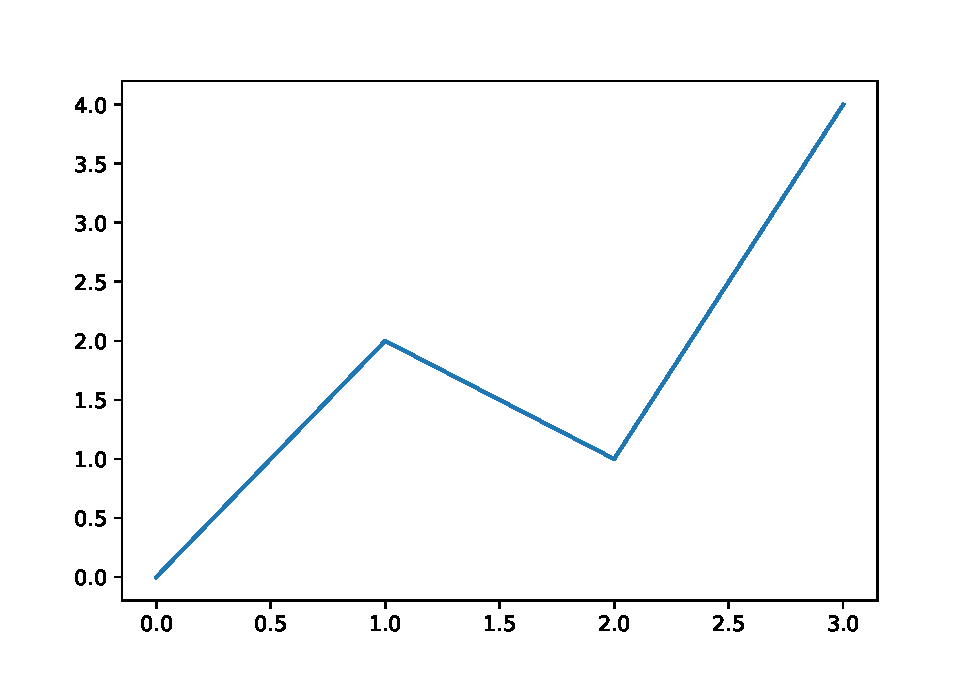
\includegraphics{202401292317-Python_files/figure-latex/unnamed-chunk-9-1.pdf}

\section{SoloLearn}\label{sololearn}

\url{https://www.sololearn.com/}

\url{https://www.sololearn.com/en/learn/courses/python-intermediate}

\section{list comprehension}\label{list-comprehension}

\url{https://www.sololearn.com/en/learn/courses/python-intermediate/lesson/1188906590?p=1}

\begin{cols}

\begin{col}{0.45\textwidth}

\begin{Shaded}
\begin{Highlighting}[]
\NormalTok{cubes }\OperatorTok{=}\NormalTok{ [i}\OperatorTok{**}\DecValTok{3} \ControlFlowTok{for}\NormalTok{ i }\KeywordTok{in} \BuiltInTok{range}\NormalTok{(}\DecValTok{5}\NormalTok{)]}

\BuiltInTok{print}\NormalTok{(cubes)}
\end{Highlighting}
\end{Shaded}

\end{col}

\begin{col}{0.10\textwidth}
~

\end{col}

\begin{col}{0.45\textwidth}

\begin{verbatim}
## [0, 1, 8, 27, 64]
\end{verbatim}

\end{col}

\end{cols}

\section{functional programming}\label{functional-programming}

\begin{itemize}
\tightlist
\item
  pure function
\item
  lambda
\item
  map
\item
  filter
\item
  generator
\item
  decorator
\item
  recursion
\item
  *args
\item
  **kwargs
\end{itemize}

\section{object-oriented programming = OOP}\label{object-oriented-programming-oop}

\begin{itemize}
\tightlist
\item
  class
\item
  inheritance
\item
  magic method
\item
  operator overloading
\item
  data hiding
\item
  static method
\item
  property
\end{itemize}

\chapter{TikZ}\label{tikz}

\begin{itemize}
\tightlist
\item
  Ti\(k\)Z

  \begin{itemize}
  \tightlist
  \item
    \hyperref[pgfplots]{PGFplots}\textsuperscript{{[}\ref{pgfplots}{]}}
  \item
    tikzplotlib\textsuperscript{{[}\ref{tikzplotlib}{]}}: \hyperref[python]{Python}\textsuperscript{{[}\ref{python}{]}} matplotlib\textsuperscript{{[}\ref{matplotlib}{]}} export to \hyperref[tikz]{TikZ}\textsuperscript{{[}\ref{tikz}{]}} .tex
  \end{itemize}
\end{itemize}

multi-column \ref{multi-column}

\begin{Shaded}
\begin{Highlighting}[]
\NormalTok{knitr}\SpecialCharTok{::}\NormalTok{opts\_chunk}\SpecialCharTok{$}\FunctionTok{set}\NormalTok{(}\AttributeTok{fig.pos =} \StringTok{"H"}\NormalTok{, }\AttributeTok{out.extra =} \StringTok{""}\NormalTok{)}
\end{Highlighting}
\end{Shaded}

\url{https://bookdown.org/yihui/rmarkdown-cookbook/html-scroll.html}

\begin{cols}

\begin{col}{0.45\textwidth}

\begin{Shaded}
\begin{Highlighting}[]
\KeywordTok{\textbackslash{}begin}\NormalTok{\{}\ExtensionTok{tikzpicture}\NormalTok{\}}
  \FunctionTok{\textbackslash{}draw}\NormalTok{ ({-}1,1){-}{-}(0,0){-}{-}(1,2);}
\KeywordTok{\textbackslash{}end}\NormalTok{\{}\ExtensionTok{tikzpicture}\NormalTok{\}}
\end{Highlighting}
\end{Shaded}

\end{col}

\begin{col}{0.10\textwidth}
~

\end{col}

\begin{col}{0.45\textwidth}

\begin{figure}[H]
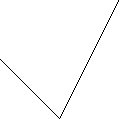
\includegraphics{202401311000-TikZ_files/figure-latex/unnamed-chunk-4-1} \end{figure}

\end{col}

\end{cols}

How to speed up bookdown generation?

\url{https://stackoverflow.com/questions/56541371/how-to-speed-up-bookdown-generation}

TikZ and PGFplots

What's the relation between packages PGFplots and TikZ?

\url{https://tex.stackexchange.com/questions/285925/whats-the-relation-between-packages-pgfplots-and-tikz}

\url{https://www.youtube.com/watch?v=bQugbYq0BVA}

\url{https://www.youtube.com/watch?v=ft4Kg9emK1k&list=PLg5nrpKdkk2DWcg3scb75AknF7DJXs8lk&index=18}

\begin{cols}

\begin{col}{0.45\textwidth}

\begin{Shaded}
\begin{Highlighting}[]
\KeywordTok{\textbackslash{}begin}\NormalTok{\{}\ExtensionTok{tikzpicture}\NormalTok{\}}
  \FunctionTok{\textbackslash{}def\textbackslash{}a}\NormalTok{\{1.5\} }\CommentTok{\% amplitude}
  \FunctionTok{\textbackslash{}def\textbackslash{}b}\NormalTok{\{2\}   }\CommentTok{\% frequency}
  \FunctionTok{\textbackslash{}draw}\NormalTok{[{-}\textgreater{}] ({-}0.2,0){-}{-}(4.2,0) node[right, font=}\FunctionTok{\textbackslash{}small}\NormalTok{] \{}\SpecialStringTok{$x$}\NormalTok{\};}
  \FunctionTok{\textbackslash{}draw}\NormalTok{[{-}\textgreater{}] (0,{-}4){-}{-}(0,0.5) node[above] \{}\SpecialStringTok{$y$}\NormalTok{\};}
  \FunctionTok{\textbackslash{}draw}\NormalTok{[domain=0:4,smooth,variable=}\FunctionTok{\textbackslash{}t}\NormalTok{,blue,thick] }
\NormalTok{    plot (\{}\FunctionTok{\textbackslash{}a}\NormalTok{ * (}\FunctionTok{\textbackslash{}b*\textbackslash{}t}\NormalTok{ {-} sin(deg(}\FunctionTok{\textbackslash{}b*\textbackslash{}t}\NormalTok{)))\},\{{-}}\FunctionTok{\textbackslash{}a}\NormalTok{ * (1 {-} cos(deg(}\FunctionTok{\textbackslash{}b*\textbackslash{}t}\NormalTok{)))\});}
  \CommentTok{\% \textbackslash{}node[above] at (2, 0.5) \{Brachistochrone Curve\};}
  \FunctionTok{\textbackslash{}node}\NormalTok{[above, font=}\FunctionTok{\textbackslash{}footnotesize}\NormalTok{] at (2, 1) \{Brachistochrone Curve\};}
  \FunctionTok{\textbackslash{}node}\NormalTok{[above, font=}\FunctionTok{\textbackslash{}footnotesize}\NormalTok{] at (2, 0) \{}\SpecialStringTok{$}\KeywordTok{\textbackslash{}begin}\NormalTok{\{}\ExtensionTok{aligned}\NormalTok{\}}
\SpecialStringTok{\& x=r(t{-}}\SpecialCharTok{\textbackslash{}sin}\SpecialStringTok{ t) }\SpecialCharTok{\textbackslash{}\textbackslash{}}
\SpecialStringTok{\& y=r(1{-}}\SpecialCharTok{\textbackslash{}cos}\SpecialStringTok{ t)}
\KeywordTok{\textbackslash{}end}\NormalTok{\{}\ExtensionTok{aligned}\NormalTok{\}}\SpecialStringTok{$}\NormalTok{\};}
\KeywordTok{\textbackslash{}end}\NormalTok{\{}\ExtensionTok{tikzpicture}\NormalTok{\}}
\end{Highlighting}
\end{Shaded}

\end{col}

\begin{col}{0.10\textwidth}
~

\end{col}

\begin{col}{0.45\textwidth}

\begin{figure}[H]
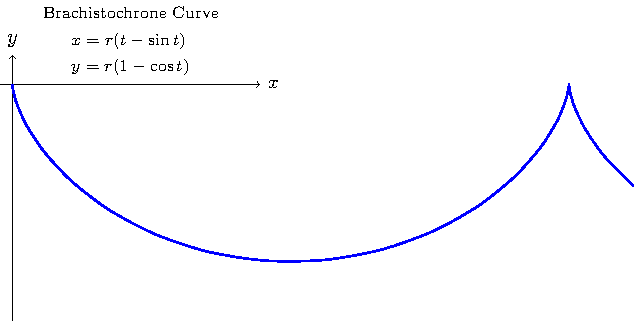
\includegraphics{202401311000-TikZ_files/figure-latex/unnamed-chunk-6-1} \caption{Brachistochrone Curve}\label{fig:unnamed-chunk-6}
\end{figure}

\end{col}

\end{cols}

\begin{figure}[H]
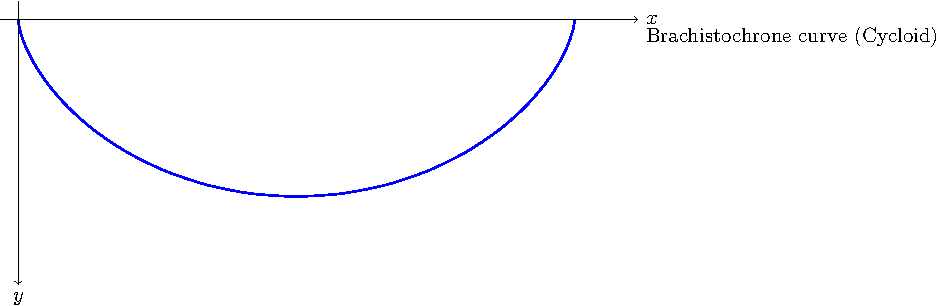
\includegraphics[width=0.9\linewidth,]{202401311000-TikZ_files/figure-latex/unnamed-chunk-7-1} \caption{Brachistochrone Curve}\label{fig:unnamed-chunk-7}
\end{figure}

\section{2D}\label{d}

\url{https://zhuanlan.zhihu.com/p/127155579?utm_psn=1741479950987960320}

\begin{Shaded}
\begin{Highlighting}[]
\KeywordTok{\textbackslash{}begin}\NormalTok{\{}\ExtensionTok{tikzpicture}\NormalTok{\}}
  \FunctionTok{\textbackslash{}draw}\NormalTok{ ({-}1,1){-}{-}(0,0){-}{-}(1,2);}
\KeywordTok{\textbackslash{}end}\NormalTok{\{}\ExtensionTok{tikzpicture}\NormalTok{\}}
\end{Highlighting}
\end{Shaded}

\begin{center}\rule{0.5\linewidth}{0.5pt}\end{center}

\begin{cols}

\begin{col}{0.45\textwidth}

\begin{Shaded}
\begin{Highlighting}[]
\KeywordTok{\textbackslash{}begin}\NormalTok{\{}\ExtensionTok{tikzpicture}\NormalTok{\}}
  \FunctionTok{\textbackslash{}draw}\NormalTok{ ({-}1,1){-}{-}(0,0){-}{-}(1,2);}
\KeywordTok{\textbackslash{}end}\NormalTok{\{}\ExtensionTok{tikzpicture}\NormalTok{\}}
\end{Highlighting}
\end{Shaded}

\end{col}

\begin{col}{0.10\textwidth}
~

\end{col}

\begin{col}{0.45\textwidth}
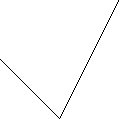
\includegraphics{202401311000-TikZ_files/figure-latex/unnamed-chunk-10-1}

\end{col}

\end{cols}

\begin{center}\rule{0.5\linewidth}{0.5pt}\end{center}

\begin{cols}

\begin{col}{0.45\textwidth}

\texttt{out.width=if\ (knitr:::is\_html\_output())\ \textquotesingle{}20\%\textquotesingle{}}

\begin{Shaded}
\begin{Highlighting}[]
\KeywordTok{\textbackslash{}begin}\NormalTok{\{}\ExtensionTok{tikzpicture}\NormalTok{\}}
  \FunctionTok{\textbackslash{}draw}\NormalTok{ ({-}1,1){-}{-}(0,0){-}{-}(1,2);}
\KeywordTok{\textbackslash{}end}\NormalTok{\{}\ExtensionTok{tikzpicture}\NormalTok{\}}
\end{Highlighting}
\end{Shaded}

\end{col}

\begin{col}{0.10\textwidth}
~

\end{col}

\begin{col}{0.45\textwidth}
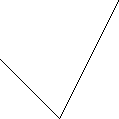
\includegraphics{202401311000-TikZ_files/figure-latex/unnamed-chunk-12-1}

\end{col}

\end{cols}

\begin{center}\rule{0.5\linewidth}{0.5pt}\end{center}

\begin{cols}

\begin{col}{0.45\textwidth}

\begin{Shaded}
\begin{Highlighting}[]
\KeywordTok{\textbackslash{}begin}\NormalTok{\{}\ExtensionTok{tikzpicture}\NormalTok{\}}
  \FunctionTok{\textbackslash{}draw}\NormalTok{[rounded corners] ({-}1,1){-}{-}(0,0){-}{-}(1,2){-}{-}({-}1,1);}
\KeywordTok{\textbackslash{}end}\NormalTok{\{}\ExtensionTok{tikzpicture}\NormalTok{\}}
\end{Highlighting}
\end{Shaded}

\end{col}

\begin{col}{0.10\textwidth}
~

\end{col}

\begin{col}{0.45\textwidth}

\begin{figure}[H]
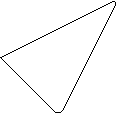
\includegraphics{202401311000-TikZ_files/figure-latex/unnamed-chunk-14-1} \caption{rounded corner pseudo-closed triangle}\label{fig:unnamed-chunk-14}
\end{figure}

\end{col}

\end{cols}

\begin{center}\rule{0.5\linewidth}{0.5pt}\end{center}

\begin{cols}

\begin{col}{0.45\textwidth}

\begin{Shaded}
\begin{Highlighting}[]
\KeywordTok{\textbackslash{}begin}\NormalTok{\{}\ExtensionTok{tikzpicture}\NormalTok{\}}
  \FunctionTok{\textbackslash{}draw}\NormalTok{[rounded corners] ({-}1,1){-}{-}(0,0){-}{-}(1,2){-}{-}cycle;}
\KeywordTok{\textbackslash{}end}\NormalTok{\{}\ExtensionTok{tikzpicture}\NormalTok{\}}
\end{Highlighting}
\end{Shaded}

\end{col}

\begin{col}{0.10\textwidth}
~

\end{col}

\begin{col}{0.45\textwidth}

\begin{figure}[H]
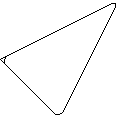
\includegraphics{202401311000-TikZ_files/figure-latex/unnamed-chunk-16-1} \caption{rounded corner triangle}\label{fig:unnamed-chunk-16}
\end{figure}

\end{col}

\end{cols}

\begin{center}\rule{0.5\linewidth}{0.5pt}\end{center}

\begin{cols}

\begin{col}{0.45\textwidth}

\begin{Shaded}
\begin{Highlighting}[]
\KeywordTok{\textbackslash{}begin}\NormalTok{\{}\ExtensionTok{tikzpicture}\NormalTok{\}}
  \FunctionTok{\textbackslash{}draw}\NormalTok{[rounded corners] ({-}1,1){-}{-}(0,0){-}{-}(1,2){-}{-}cycle;}
  \FunctionTok{\textbackslash{}draw}\NormalTok{[rounded corners] ({-}1,1){-}{-}(0,0){-}{-}(1,2){-}{-}({-}1,1);}
\KeywordTok{\textbackslash{}end}\NormalTok{\{}\ExtensionTok{tikzpicture}\NormalTok{\}}
\end{Highlighting}
\end{Shaded}

\end{col}

\begin{col}{0.10\textwidth}
~

\end{col}

\begin{col}{0.45\textwidth}

\begin{figure}[H]
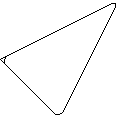
\includegraphics{202401311000-TikZ_files/figure-latex/unnamed-chunk-18-1} \caption{triangle vs. pseudo-closed triangle}\label{fig:unnamed-chunk-18}
\end{figure}

\end{col}

\end{cols}

\begin{center}\rule{0.5\linewidth}{0.5pt}\end{center}

\begin{cols}

\begin{col}{0.45\textwidth}

\begin{Shaded}
\begin{Highlighting}[]
\KeywordTok{\textbackslash{}begin}\NormalTok{\{}\ExtensionTok{tikzpicture}\NormalTok{\}}
  \FunctionTok{\textbackslash{}draw}\NormalTok{ (0,0) rectangle (4,2);}
\KeywordTok{\textbackslash{}end}\NormalTok{\{}\ExtensionTok{tikzpicture}\NormalTok{\}}
\end{Highlighting}
\end{Shaded}

\end{col}

\begin{col}{0.10\textwidth}
~

\end{col}

\begin{col}{0.45\textwidth}

\begin{figure}[H]
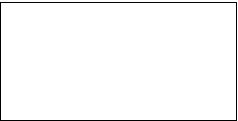
\includegraphics{202401311000-TikZ_files/figure-latex/unnamed-chunk-20-1} \caption{rectangle}\label{fig:unnamed-chunk-20}
\end{figure}

\end{col}

\end{cols}

\begin{center}\rule{0.5\linewidth}{0.5pt}\end{center}

\begin{cols}

\begin{col}{0.45\textwidth}

\begin{Shaded}
\begin{Highlighting}[]
\KeywordTok{\textbackslash{}begin}\NormalTok{\{}\ExtensionTok{tikzpicture}\NormalTok{\}}
  \FunctionTok{\textbackslash{}draw}\NormalTok{ (0,0) rectangle (2,2);}
\KeywordTok{\textbackslash{}end}\NormalTok{\{}\ExtensionTok{tikzpicture}\NormalTok{\}}
\end{Highlighting}
\end{Shaded}

\end{col}

\begin{col}{0.10\textwidth}
~

\end{col}

\begin{col}{0.45\textwidth}

\begin{figure}[H]

\includegraphics{202401311000-TikZ_files/figure-latex/unnamed-chunk-22-1} \caption{square}\label{fig:unnamed-chunk-22}
\end{figure}

\end{col}

\end{cols}

\begin{center}\rule{0.5\linewidth}{0.5pt}\end{center}

\begin{cols}

\begin{col}{0.45\textwidth}

\begin{Shaded}
\begin{Highlighting}[]
\KeywordTok{\textbackslash{}begin}\NormalTok{\{}\ExtensionTok{tikzpicture}\NormalTok{\}}
  \FunctionTok{\textbackslash{}draw}\NormalTok{ (0,0) circle (1);}
\KeywordTok{\textbackslash{}end}\NormalTok{\{}\ExtensionTok{tikzpicture}\NormalTok{\}}
\end{Highlighting}
\end{Shaded}

\end{col}

\begin{col}{0.10\textwidth}
~

\end{col}

\begin{col}{0.45\textwidth}

\begin{figure}[H]
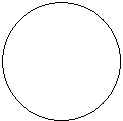
\includegraphics{202401311000-TikZ_files/figure-latex/unnamed-chunk-24-1} \caption{circle}\label{fig:unnamed-chunk-24}
\end{figure}

\end{col}

\end{cols}

\begin{center}\rule{0.5\linewidth}{0.5pt}\end{center}

\begin{cols}

\begin{col}{0.45\textwidth}

\begin{Shaded}
\begin{Highlighting}[]
\KeywordTok{\textbackslash{}begin}\NormalTok{\{}\ExtensionTok{tikzpicture}\NormalTok{\}}
  \FunctionTok{\textbackslash{}draw}\NormalTok{ (0,0) circle (1);}
  \FunctionTok{\textbackslash{}draw}\NormalTok{ (0,0) rectangle (2,2);}
\KeywordTok{\textbackslash{}end}\NormalTok{\{}\ExtensionTok{tikzpicture}\NormalTok{\}}
\end{Highlighting}
\end{Shaded}

\end{col}

\begin{col}{0.10\textwidth}
~

\end{col}

\begin{col}{0.45\textwidth}

\begin{figure}[H]
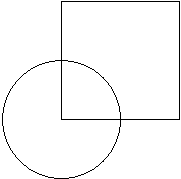
\includegraphics{202401311000-TikZ_files/figure-latex/unnamed-chunk-26-1} \caption{circle and square}\label{fig:unnamed-chunk-26}
\end{figure}

\end{col}

\end{cols}

\begin{center}\rule{0.5\linewidth}{0.5pt}\end{center}

\begin{cols}

\begin{col}{0.45\textwidth}

\begin{Shaded}
\begin{Highlighting}[]
\KeywordTok{\textbackslash{}begin}\NormalTok{\{}\ExtensionTok{tikzpicture}\NormalTok{\}}
  \FunctionTok{\textbackslash{}draw}\NormalTok{ (1,1) ellipse (2 and 1);}
\KeywordTok{\textbackslash{}end}\NormalTok{\{}\ExtensionTok{tikzpicture}\NormalTok{\}}
\end{Highlighting}
\end{Shaded}

\end{col}

\begin{col}{0.10\textwidth}
~

\end{col}

\begin{col}{0.45\textwidth}

\begin{figure}[H]
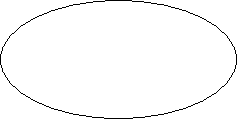
\includegraphics{202401311000-TikZ_files/figure-latex/unnamed-chunk-28-1} \caption{ellipse}\label{fig:unnamed-chunk-28}
\end{figure}

\end{col}

\end{cols}

\begin{center}\rule{0.5\linewidth}{0.5pt}\end{center}

\begin{cols}

\begin{col}{0.45\textwidth}

\begin{Shaded}
\begin{Highlighting}[]
\KeywordTok{\textbackslash{}begin}\NormalTok{\{}\ExtensionTok{tikzpicture}\NormalTok{\}}
  \FunctionTok{\textbackslash{}draw}\NormalTok{ (1 ,1) arc (0:270:1);}
  \FunctionTok{\textbackslash{}draw}\NormalTok{ (6 ,1) arc (0:270:2 and 1);}
\KeywordTok{\textbackslash{}end}\NormalTok{\{}\ExtensionTok{tikzpicture}\NormalTok{\}}
\end{Highlighting}
\end{Shaded}

\end{col}

\begin{col}{0.10\textwidth}
~

\end{col}

\begin{col}{0.45\textwidth}

\begin{figure}[H]
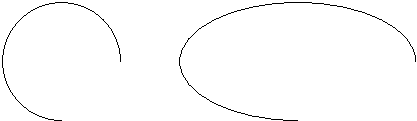
\includegraphics{202401311000-TikZ_files/figure-latex/unnamed-chunk-30-1} \caption{circle and ellipse arcs}\label{fig:unnamed-chunk-30}
\end{figure}

\end{col}

\end{cols}

\begin{center}\rule{0.5\linewidth}{0.5pt}\end{center}

\begin{cols}

\begin{col}{0.45\textwidth}

\begin{Shaded}
\begin{Highlighting}[]
\KeywordTok{\textbackslash{}begin}\NormalTok{\{}\ExtensionTok{tikzpicture}\NormalTok{\}}
  \FunctionTok{\textbackslash{}draw}\NormalTok{ ({-}1,1) parabola bend (0,0) (2,4);}
\KeywordTok{\textbackslash{}end}\NormalTok{\{}\ExtensionTok{tikzpicture}\NormalTok{\}}
\end{Highlighting}
\end{Shaded}

\end{col}

\begin{col}{0.10\textwidth}
~

\end{col}

\begin{col}{0.45\textwidth}

\begin{figure}[H]
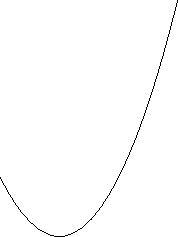
\includegraphics{202401311000-TikZ_files/figure-latex/unnamed-chunk-32-1} \caption{parabola arc}\label{fig:unnamed-chunk-32}
\end{figure}

\end{col}

\end{cols}

\begin{center}\rule{0.5\linewidth}{0.5pt}\end{center}

\begin{cols}

\begin{col}{0.45\textwidth}

\begin{Shaded}
\begin{Highlighting}[]
\KeywordTok{\textbackslash{}begin}\NormalTok{\{}\ExtensionTok{tikzpicture}\NormalTok{\}}
  \FunctionTok{\textbackslash{}draw}\NormalTok{ ({-}1,1) parabola bend (0,0) (2,4);}
  \FunctionTok{\textbackslash{}filldraw}
\NormalTok{    ({-}1,1) circle (.05)}
\NormalTok{    ( 0,0) circle (.05)}
\NormalTok{    ( 1,1) circle (.05)}
\NormalTok{    ( 2,4) circle (.05);}
\KeywordTok{\textbackslash{}end}\NormalTok{\{}\ExtensionTok{tikzpicture}\NormalTok{\}}
\end{Highlighting}
\end{Shaded}

\end{col}

\begin{col}{0.10\textwidth}
~

\end{col}

\begin{col}{0.45\textwidth}

\begin{figure}[H]
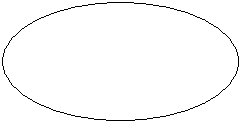
\includegraphics{202401311000-TikZ_files/figure-latex/unnamed-chunk-34-1} \caption{parabola arc with points}\label{fig:unnamed-chunk-34}
\end{figure}

\end{col}

\end{cols}

\begin{center}\rule{0.5\linewidth}{0.5pt}\end{center}

\begin{cols}

\begin{col}{0.45\textwidth}

\begin{Shaded}
\begin{Highlighting}[]
\KeywordTok{\textbackslash{}begin}\NormalTok{\{}\ExtensionTok{tikzpicture}\NormalTok{\}}
  \FunctionTok{\textbackslash{}draw}\NormalTok{[step=20pt] (0,0) grid (3,2);}
  \FunctionTok{\textbackslash{}draw}\NormalTok{[help lines ,step=20pt] (4,0) grid (7,2);}
\KeywordTok{\textbackslash{}end}\NormalTok{\{}\ExtensionTok{tikzpicture}\NormalTok{\}}
\end{Highlighting}
\end{Shaded}

\end{col}

\begin{col}{0.10\textwidth}
~

\end{col}

\begin{col}{0.45\textwidth}

\begin{figure}[H]

\includegraphics{202401311000-TikZ_files/figure-latex/unnamed-chunk-36-1} \caption{grid and help lines}\label{fig:unnamed-chunk-36}
\end{figure}

\end{col}

\end{cols}

\begin{center}\rule{0.5\linewidth}{0.5pt}\end{center}

\begin{cols}

\begin{col}{0.45\textwidth}

\begin{Shaded}
\begin{Highlighting}[]
\KeywordTok{\textbackslash{}begin}\NormalTok{\{}\ExtensionTok{tikzpicture}\NormalTok{\}[scale=0.25]}
  \FunctionTok{\textbackslash{}draw}\NormalTok{[{-}\textgreater{}] (0,0){-}{-}(9,0);}
  \FunctionTok{\textbackslash{}draw}\NormalTok{[\textless{}{-}] (0,1){-}{-}(9,1);}
  \FunctionTok{\textbackslash{}draw}\NormalTok{[\textless{}{-}\textgreater{}] (0,2){-}{-}(9,2);}
  \FunctionTok{\textbackslash{}draw}\NormalTok{[\textgreater{}{-}\textgreater{}\textgreater{}] (0,3){-}{-}(9,3);}
  \FunctionTok{\textbackslash{}draw}\NormalTok{[|\textless{}{-}\textgreater{}|] (0,4){-}{-}(9,4);}
\KeywordTok{\textbackslash{}end}\NormalTok{\{}\ExtensionTok{tikzpicture}\NormalTok{\}}
\end{Highlighting}
\end{Shaded}

\end{col}

\begin{col}{0.10\textwidth}
~

\end{col}

\begin{col}{0.45\textwidth}

\begin{figure}[H]
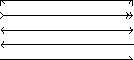
\includegraphics{202401311000-TikZ_files/figure-latex/unnamed-chunk-38-1} \caption{arrows}\label{fig:unnamed-chunk-38}
\end{figure}

\end{col}

\end{cols}

\begin{center}\rule{0.5\linewidth}{0.5pt}\end{center}

\begin{cols}

\begin{col}{0.45\textwidth}

\begin{Shaded}
\begin{Highlighting}[]
\KeywordTok{\textbackslash{}begin}\NormalTok{\{}\ExtensionTok{tikzpicture}\NormalTok{\}}
  \FunctionTok{\textbackslash{}draw}\NormalTok{[line width =2pt] (0,6){-}{-}(9,6); }
  \FunctionTok{\textbackslash{}draw}\NormalTok{[dotted]          (0,5){-}{-}(9,5); }
  \FunctionTok{\textbackslash{}draw}\NormalTok{[densely dotted]  (0,4){-}{-}(9,4); }
  \FunctionTok{\textbackslash{}draw}\NormalTok{[loosely dotted]  (0,3){-}{-}(9,3); }
  \FunctionTok{\textbackslash{}draw}\NormalTok{[dashed]          (0,2){-}{-}(9,2); }
  \FunctionTok{\textbackslash{}draw}\NormalTok{[densely dashed]  (0,1){-}{-}(9,1); }
  \FunctionTok{\textbackslash{}draw}\NormalTok{[loosely dashed]  (0,0){-}{-}(9,0);}
\KeywordTok{\textbackslash{}end}\NormalTok{\{}\ExtensionTok{tikzpicture}\NormalTok{\}}
\end{Highlighting}
\end{Shaded}

\end{col}

\begin{col}{0.10\textwidth}
~

\end{col}

\begin{col}{0.45\textwidth}

\begin{figure}[H]
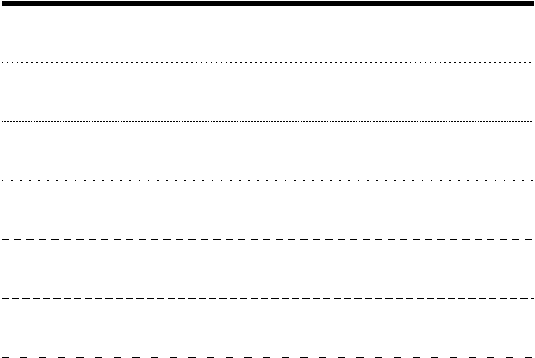
\includegraphics{202401311000-TikZ_files/figure-latex/unnamed-chunk-40-1} \caption{lines}\label{fig:unnamed-chunk-40}
\end{figure}

\end{col}

\end{cols}

\begin{center}\rule{0.5\linewidth}{0.5pt}\end{center}

\begin{cols}

\begin{col}{0.45\textwidth}

\begin{Shaded}
\begin{Highlighting}[]
\KeywordTok{\textbackslash{}begin}\NormalTok{\{}\ExtensionTok{tikzpicture}\NormalTok{\}[dline/.style=\{color= blue, line width=2pt\}]}
  \FunctionTok{\textbackslash{}draw}\NormalTok{[dline] (0,0){-}{-}(9,0); }
\KeywordTok{\textbackslash{}end}\NormalTok{\{}\ExtensionTok{tikzpicture}\NormalTok{\}}
\end{Highlighting}
\end{Shaded}

\end{col}

\begin{col}{0.10\textwidth}
~

\end{col}

\begin{col}{0.45\textwidth}

\begin{figure}[H]

\includegraphics{202401311000-TikZ_files/figure-latex/unnamed-chunk-42-1} \caption{head styling}\label{fig:unnamed-chunk-42}
\end{figure}

\end{col}

\end{cols}

\begin{center}\rule{0.5\linewidth}{0.5pt}\end{center}

\begin{cols}

\begin{col}{0.45\textwidth}

\begin{Shaded}
\begin{Highlighting}[]
\KeywordTok{\textbackslash{}begin}\NormalTok{\{}\ExtensionTok{tikzpicture}\NormalTok{\}}
  \FunctionTok{\textbackslash{}draw}\NormalTok{ (0,0) rectangle (2,2);}
  \FunctionTok{\textbackslash{}draw}\NormalTok{[shift=\{( 3, 0)\}] (0,0) rectangle (2,2);}
  \FunctionTok{\textbackslash{}draw}\NormalTok{[shift=\{( 0, 3)\}] (0,0) rectangle (2,2);}
  \FunctionTok{\textbackslash{}draw}\NormalTok{[shift=\{( 0,{-}3)\}] (0,0) rectangle (2,2);}
  \FunctionTok{\textbackslash{}draw}\NormalTok{[shift=\{({-}3, 0)\}] (0,0) rectangle (2,2);}
  \FunctionTok{\textbackslash{}draw}\NormalTok{[shift=\{( 3, 3)\}] (0,0) rectangle (2,2);}
  \FunctionTok{\textbackslash{}draw}\NormalTok{[shift=\{({-}3, 3)\}] (0,0) rectangle (2,2);}
  \FunctionTok{\textbackslash{}draw}\NormalTok{[shift=\{( 3,{-}3)\}] (0,0) rectangle (2,2);}
  \FunctionTok{\textbackslash{}draw}\NormalTok{[shift=\{({-}3,{-}3)\}] (0,0) rectangle (2,2);}
\KeywordTok{\textbackslash{}end}\NormalTok{\{}\ExtensionTok{tikzpicture}\NormalTok{\}}
\end{Highlighting}
\end{Shaded}

\end{col}

\begin{col}{0.10\textwidth}
~

\end{col}

\begin{col}{0.45\textwidth}

\begin{figure}[H]

\includegraphics{202401311000-TikZ_files/figure-latex/unnamed-chunk-44-1} \caption{transform: shift}\label{fig:unnamed-chunk-44}
\end{figure}

\end{col}

\end{cols}

\begin{center}\rule{0.5\linewidth}{0.5pt}\end{center}

\begin{cols}

\begin{col}{0.45\textwidth}

\begin{Shaded}
\begin{Highlighting}[]
\KeywordTok{\textbackslash{}begin}\NormalTok{\{}\ExtensionTok{tikzpicture}\NormalTok{\}}
  \FunctionTok{\textbackslash{}draw}\NormalTok{ (0,0) rectangle (2,2);}
  \FunctionTok{\textbackslash{}draw}\NormalTok{[xshift= 100pt] (0,0) rectangle (2,2);}
  \FunctionTok{\textbackslash{}draw}\NormalTok{[xshift={-}100pt] (0,0) rectangle (2,2);}
  \FunctionTok{\textbackslash{}draw}\NormalTok{[yshift= 100pt] (0,0) rectangle (2,2);}
  \FunctionTok{\textbackslash{}draw}\NormalTok{[yshift={-}100pt] (0,0) rectangle (2,2);}
\KeywordTok{\textbackslash{}end}\NormalTok{\{}\ExtensionTok{tikzpicture}\NormalTok{\}}
\end{Highlighting}
\end{Shaded}

\end{col}

\begin{col}{0.10\textwidth}
~

\end{col}

\begin{col}{0.45\textwidth}

\begin{figure}[H]
\includegraphics{202401311000-TikZ_files/figure-latex/unnamed-chunk-46-1} \caption{transform: shift x, y}\label{fig:unnamed-chunk-46}
\end{figure}

\end{col}

\end{cols}

\begin{center}\rule{0.5\linewidth}{0.5pt}\end{center}

\begin{cols}

\begin{col}{0.45\textwidth}

\begin{Shaded}
\begin{Highlighting}[]
\KeywordTok{\textbackslash{}begin}\NormalTok{\{}\ExtensionTok{tikzpicture}\NormalTok{\}}
  \FunctionTok{\textbackslash{}draw}\NormalTok{ (0,0) rectangle (2,2);}
  \FunctionTok{\textbackslash{}draw}\NormalTok{[xshift= 100pt, xscale=1.5] (0,0) rectangle (2,2);}
  \FunctionTok{\textbackslash{}draw}\NormalTok{[yshift= 100pt, xscale=0.5] (0,0) rectangle (2,2);}
  \FunctionTok{\textbackslash{}draw}\NormalTok{[xshift={-}100pt, yscale=1.5] (0,0) rectangle (2,2);}
  \FunctionTok{\textbackslash{}draw}\NormalTok{[yshift={-}100pt, yscale=0.5] (0,0) rectangle (2,2);}
\KeywordTok{\textbackslash{}end}\NormalTok{\{}\ExtensionTok{tikzpicture}\NormalTok{\}}
\end{Highlighting}
\end{Shaded}

\end{col}

\begin{col}{0.10\textwidth}
~

\end{col}

\begin{col}{0.45\textwidth}

\begin{figure}[H]
\includegraphics{202401311000-TikZ_files/figure-latex/unnamed-chunk-48-1} \caption{transform: scale x, y}\label{fig:unnamed-chunk-48}
\end{figure}

\end{col}

\end{cols}

\begin{center}\rule{0.5\linewidth}{0.5pt}\end{center}

\begin{cols}

\begin{col}{0.45\textwidth}

\begin{Shaded}
\begin{Highlighting}[]
\KeywordTok{\textbackslash{}begin}\NormalTok{\{}\ExtensionTok{tikzpicture}\NormalTok{\}}
  \FunctionTok{\textbackslash{}draw}\NormalTok{ (0,0) rectangle (2,2);}
  \FunctionTok{\textbackslash{}draw}\NormalTok{[xshift= 100pt, xscale=1.5] (0,0) rectangle (2,2);}
  \FunctionTok{\textbackslash{}draw}\NormalTok{[yshift= 100pt, yscale=1.5] (0,0) rectangle (2,2);}
  \FunctionTok{\textbackslash{}draw}\NormalTok{[xshift={-}100pt, xscale=0.5] (0,0) rectangle (2,2);}
  \FunctionTok{\textbackslash{}draw}\NormalTok{[yshift={-}100pt, yscale=0.5] (0,0) rectangle (2,2);}
\KeywordTok{\textbackslash{}end}\NormalTok{\{}\ExtensionTok{tikzpicture}\NormalTok{\}}
\end{Highlighting}
\end{Shaded}

\end{col}

\begin{col}{0.10\textwidth}
~

\end{col}

\begin{col}{0.45\textwidth}

\begin{figure}[H]
\includegraphics{202401311000-TikZ_files/figure-latex/unnamed-chunk-50-1} \caption{transform: scale}\label{fig:unnamed-chunk-50}
\end{figure}

\end{col}

\end{cols}

\begin{center}\rule{0.5\linewidth}{0.5pt}\end{center}

\begin{cols}

\begin{col}{0.45\textwidth}

\begin{Shaded}
\begin{Highlighting}[]
\KeywordTok{\textbackslash{}begin}\NormalTok{\{}\ExtensionTok{tikzpicture}\NormalTok{\}}
  \FunctionTok{\textbackslash{}draw}\NormalTok{ (0,0) rectangle (2,2);}
  \FunctionTok{\textbackslash{}draw}\NormalTok{[xshift=125pt,rotate=45] (0,0) rectangle (2,2);}
  \FunctionTok{\textbackslash{}draw}\NormalTok{[xshift=175pt,rotate around=\{45:(2 ,2)\}] (0,0) rectangle (2,2);}
\KeywordTok{\textbackslash{}end}\NormalTok{\{}\ExtensionTok{tikzpicture}\NormalTok{\}}
\end{Highlighting}
\end{Shaded}

\end{col}

\begin{col}{0.10\textwidth}
~

\end{col}

\begin{col}{0.45\textwidth}

\begin{figure}[H]
\includegraphics{202401311000-TikZ_files/figure-latex/unnamed-chunk-52-1} \caption{transform: rotate}\label{fig:unnamed-chunk-52}
\end{figure}

\end{col}

\end{cols}

\begin{center}\rule{0.5\linewidth}{0.5pt}\end{center}

\begin{cols}

\begin{col}{0.45\textwidth}

\begin{Shaded}
\begin{Highlighting}[]
\KeywordTok{\textbackslash{}begin}\NormalTok{\{}\ExtensionTok{tikzpicture}\NormalTok{\}}
  \FunctionTok{\textbackslash{}draw}\NormalTok{ (0,0) rectangle (2,2);}
  \FunctionTok{\textbackslash{}draw}\NormalTok{[xshift=70pt,xslant=1] (0,0) rectangle (2,2);}
  \FunctionTok{\textbackslash{}draw}\NormalTok{[yshift=70pt,yslant=1] (0,0) rectangle (2,2);}
\KeywordTok{\textbackslash{}end}\NormalTok{\{}\ExtensionTok{tikzpicture}\NormalTok{\}}
\end{Highlighting}
\end{Shaded}

\end{col}

\begin{col}{0.10\textwidth}
~

\end{col}

\begin{col}{0.45\textwidth}

\begin{figure}[H]
\includegraphics{202401311000-TikZ_files/figure-latex/unnamed-chunk-54-1} \caption{transform: slant}\label{fig:unnamed-chunk-54}
\end{figure}

\end{col}

\end{cols}

\begin{center}\rule{0.5\linewidth}{0.5pt}\end{center}

\begin{cols}

\begin{col}{0.45\textwidth}

\begin{Shaded}
\begin{Highlighting}[]
\FunctionTok{\textbackslash{}tikzset}\NormalTok{\{}
\NormalTok{  box/.style=\{}
\NormalTok{    draw=blue,}
\NormalTok{    rectangle,}
\NormalTok{    rounded corners=5pt,}
\NormalTok{    minimum width=50pt,}
\NormalTok{    minimum height=20pt,}
\NormalTok{    inner sep=5pt}
\NormalTok{  \}}
\NormalTok{\}}
\KeywordTok{\textbackslash{}begin}\NormalTok{\{}\ExtensionTok{tikzpicture}\NormalTok{\}}
  \FunctionTok{\textbackslash{}node}\NormalTok{[box] (1) at (0,0) \{1\};}
  \FunctionTok{\textbackslash{}node}\NormalTok{[box] (2) at (4,0) \{2\};}
  \FunctionTok{\textbackslash{}node}\NormalTok{[box] (3) at (8,0) \{3\};}
  \FunctionTok{\textbackslash{}draw}\NormalTok{[{-}\textgreater{}] (1){-}{-}(2);}
  \FunctionTok{\textbackslash{}draw}\NormalTok{[{-}\textgreater{}] (2){-}{-}(3);}
  \FunctionTok{\textbackslash{}node}\NormalTok{ at (2,1) \{a\};}
  \FunctionTok{\textbackslash{}node}\NormalTok{ at (6,1) \{b\};}
\KeywordTok{\textbackslash{}end}\NormalTok{\{}\ExtensionTok{tikzpicture}\NormalTok{\}}
\end{Highlighting}
\end{Shaded}

\end{col}

\begin{col}{0.10\textwidth}
~

\end{col}

\begin{col}{0.45\textwidth}

\begin{figure}[H]
\includegraphics{202401311000-TikZ_files/figure-latex/unnamed-chunk-56-1} \caption{flowchart}\label{fig:unnamed-chunk-56}
\end{figure}

\end{col}

\end{cols}

\begin{center}\rule{0.5\linewidth}{0.5pt}\end{center}

\begin{cols}

\begin{col}{0.45\textwidth}

\begin{Shaded}
\begin{Highlighting}[]
\FunctionTok{\textbackslash{}tikzset}\NormalTok{\{}
\NormalTok{  box/.style=\{}
\NormalTok{    draw=blue,}
\NormalTok{    fill=blue!20,}
\NormalTok{    rectangle,}
\NormalTok{    rounded corners=5pt,}
\NormalTok{    minimum height=20pt,}
\NormalTok{    inner sep=5pt}
\NormalTok{  \}}
\NormalTok{\}}
\KeywordTok{\textbackslash{}begin}\NormalTok{\{}\ExtensionTok{tikzpicture}\NormalTok{\}}
  \FunctionTok{\textbackslash{}node}\NormalTok{[box] \{1\}}
\NormalTok{      child \{node[box] \{2\}\}}
\NormalTok{      child \{node[box] \{3\}}
\NormalTok{          child \{node[box] \{4\}\}}
\NormalTok{          child \{node[box] \{5\}\}}
\NormalTok{          child \{node[box] \{6\}\}}
\NormalTok{      \};}
\KeywordTok{\textbackslash{}end}\NormalTok{\{}\ExtensionTok{tikzpicture}\NormalTok{\}}
\end{Highlighting}
\end{Shaded}

\end{col}

\begin{col}{0.10\textwidth}
~

\end{col}

\begin{col}{0.45\textwidth}

\begin{figure}[H]
\includegraphics{202401311000-TikZ_files/figure-latex/unnamed-chunk-58-1} \caption{tree}\label{fig:unnamed-chunk-58}
\end{figure}

\end{col}

\end{cols}

\begin{center}\rule{0.5\linewidth}{0.5pt}\end{center}

\begin{cols}

\begin{col}{0.45\textwidth}

\begin{Shaded}
\begin{Highlighting}[]
\KeywordTok{\textbackslash{}begin}\NormalTok{\{}\ExtensionTok{tikzpicture}\NormalTok{\}}
  \FunctionTok{\textbackslash{}draw}\NormalTok{[{-}\textgreater{}] ({-}0.2,0){-}{-}(6,0) node[right] \{}\SpecialStringTok{$x$}\NormalTok{\};}
  \FunctionTok{\textbackslash{}draw}\NormalTok{[{-}\textgreater{}] (0,{-}0.2){-}{-}(0,6) node[above] \{}\SpecialStringTok{$f(x)$}\NormalTok{\};}
  \FunctionTok{\textbackslash{}draw}\NormalTok{[domain=0:4] plot (}\FunctionTok{\textbackslash{}x}\NormalTok{ ,\{0.1* exp(}\FunctionTok{\textbackslash{}x}\NormalTok{)\}) node[right] \{}\SpecialStringTok{$f(x)=}\SpecialCharTok{\textbackslash{}frac}\SpecialStringTok{\{1\}\{10\}e\^{}x$}\NormalTok{\};}
\KeywordTok{\textbackslash{}end}\NormalTok{\{}\ExtensionTok{tikzpicture}\NormalTok{\}}
\end{Highlighting}
\end{Shaded}

\end{col}

\begin{col}{0.10\textwidth}
~

\end{col}

\begin{col}{0.45\textwidth}

\begin{figure}[H]
\includegraphics{202401311000-TikZ_files/figure-latex/unnamed-chunk-60-1} \caption{function plot}\label{fig:unnamed-chunk-60}
\end{figure}

\end{col}

\end{cols}

\url{https://stackoverflow.com/questions/64897575/tikz-libraries-in-bookdown}

It turns out that you can simply put the \texttt{\textbackslash{}usetikzlibrary\{...\}} command directly before the \texttt{\textbackslash{}begin\{tikzpicture\}} and everything works fine :)

\url{https://stackoverflow.com/questions/56211210/r-markdown-document-with-html-docx-output-using-latex-package-bbm}

\url{https://tex.stackexchange.com/questions/171711/how-to-include-latex-package-in-r-markdown}

\section{3D}\label{d-1}

\url{https://zhuanlan.zhihu.com/p/431732330?utm_psn=1741857547550638080}

\url{https://github.com/RRWWW/Stereometry}

\begin{cols}

\begin{col}{0.45\textwidth}

\begin{Shaded}
\begin{Highlighting}[]
\KeywordTok{\textbackslash{}begin}\NormalTok{\{}\ExtensionTok{tikzpicture}\NormalTok{\}}
  \FunctionTok{\textbackslash{}coordinate}\NormalTok{ (A) at ( 1, 1, 1);}
  \FunctionTok{\textbackslash{}coordinate}\NormalTok{ (B) at ( 1, 1,{-}1);}
  \FunctionTok{\textbackslash{}coordinate}\NormalTok{ (C) at ( 1,{-}1,{-}1);}
  \FunctionTok{\textbackslash{}coordinate}\NormalTok{ (D) at ( 1,{-}1, 1);}
  \FunctionTok{\textbackslash{}coordinate}\NormalTok{ (E) at ({-}1,{-}1, 1);}
  \FunctionTok{\textbackslash{}coordinate}\NormalTok{ (F) at ({-}1,{-}1,{-}1);}
  \FunctionTok{\textbackslash{}coordinate}\NormalTok{ (G) at ({-}1, 1,{-}1);}
  \FunctionTok{\textbackslash{}coordinate}\NormalTok{ (H) at ({-}1, 1, 1);}
  \FunctionTok{\textbackslash{}draw}\NormalTok{ (A) node[right=1pt] \{}\SpecialStringTok{$A$}\NormalTok{\}{-}{-}}
\NormalTok{        (B) node[right=1pt] \{}\SpecialStringTok{$B$}\NormalTok{\}{-}{-}}
\NormalTok{        (C) node[right=1pt] \{}\SpecialStringTok{$C$}\NormalTok{\}{-}{-}}
\NormalTok{        (D) node[right=1pt] \{}\SpecialStringTok{$D$}\NormalTok{\}{-}{-}}
\NormalTok{        (E) node[left= 1pt] \{}\SpecialStringTok{$E$}\NormalTok{\}{-}{-}}
\NormalTok{        (F) node[right=1pt] \{}\SpecialStringTok{$F$}\NormalTok{\}{-}{-}}
\NormalTok{        (G) node[right=1pt] \{}\SpecialStringTok{$G$}\NormalTok{\}{-}{-}}
\NormalTok{        (H) node[left= 1pt] \{}\SpecialStringTok{$H$}\NormalTok{\}{-}{-}}
\NormalTok{        (A) node[right=1pt] \{}\SpecialStringTok{$A$}\NormalTok{\};}
\KeywordTok{\textbackslash{}end}\NormalTok{\{}\ExtensionTok{tikzpicture}\NormalTok{\}}
\end{Highlighting}
\end{Shaded}

\end{col}

\begin{col}{0.10\textwidth}
~

\end{col}

\begin{col}{0.45\textwidth}

\begin{figure}[H]
\includegraphics{202401311000-TikZ_files/figure-latex/unnamed-chunk-62-1} \caption{cube}\label{fig:unnamed-chunk-62}
\end{figure}

\end{col}

\end{cols}

\begin{center}\rule{0.5\linewidth}{0.5pt}\end{center}

\begin{cols}

\begin{col}{0.45\textwidth}

\begin{Shaded}
\begin{Highlighting}[]
\FunctionTok{\textbackslash{}usetikzlibrary}\NormalTok{\{patterns\}}
\FunctionTok{\textbackslash{}usetikzlibrary}\NormalTok{\{3d,calc\}}
\FunctionTok{\textbackslash{}tdplotsetmaincoords}\NormalTok{\{45\}\{45\}}
\KeywordTok{\textbackslash{}begin}\NormalTok{\{}\ExtensionTok{tikzpicture}\NormalTok{\}[tdplot\_main\_coords]}
  \FunctionTok{\textbackslash{}coordinate}\NormalTok{ (A) at ( 1, 1, 1);}
  \FunctionTok{\textbackslash{}coordinate}\NormalTok{ (B) at ( 1, 1,{-}1);}
  \FunctionTok{\textbackslash{}coordinate}\NormalTok{ (C) at ( 1,{-}1,{-}1);}
  \FunctionTok{\textbackslash{}coordinate}\NormalTok{ (D) at ( 1,{-}1, 1);}
  \FunctionTok{\textbackslash{}coordinate}\NormalTok{ (E) at ({-}1,{-}1, 1);}
  \FunctionTok{\textbackslash{}coordinate}\NormalTok{ (F) at ({-}1,{-}1,{-}1);}
  \FunctionTok{\textbackslash{}coordinate}\NormalTok{ (G) at ({-}1, 1,{-}1);}
  \FunctionTok{\textbackslash{}coordinate}\NormalTok{ (H) at ({-}1, 1, 1);}
  \FunctionTok{\textbackslash{}draw}\NormalTok{ (A) node[right=1pt] \{}\SpecialStringTok{$A$}\NormalTok{\}{-}{-}}
\NormalTok{        (B) node[right=1pt] \{}\SpecialStringTok{$B$}\NormalTok{\}{-}{-}}
\NormalTok{        (C) node[right=1pt] \{}\SpecialStringTok{$C$}\NormalTok{\}{-}{-}}
\NormalTok{        (D) node[right=1pt] \{}\SpecialStringTok{$D$}\NormalTok{\}{-}{-}}
\NormalTok{        (E) node[left= 1pt] \{}\SpecialStringTok{$E$}\NormalTok{\}{-}{-}}
\NormalTok{        (F) node[right=1pt] \{}\SpecialStringTok{$F$}\NormalTok{\}{-}{-}}
\NormalTok{        (G) node[right=1pt] \{}\SpecialStringTok{$G$}\NormalTok{\}{-}{-}}
\NormalTok{        (H) node[left= 1pt] \{}\SpecialStringTok{$H$}\NormalTok{\}{-}{-}}
\NormalTok{        (A) node[right=1pt] \{}\SpecialStringTok{$A$}\NormalTok{\};}
\KeywordTok{\textbackslash{}end}\NormalTok{\{}\ExtensionTok{tikzpicture}\NormalTok{\}}
\end{Highlighting}
\end{Shaded}

\end{col}

\begin{col}{0.10\textwidth}
~

\end{col}

\begin{col}{0.45\textwidth}

\begin{figure}[H]
\includegraphics{202401311000-TikZ_files/figure-latex/unnamed-chunk-64-1} \caption{cube rotate}\label{fig:unnamed-chunk-64}
\end{figure}

\end{col}

\end{cols}

\begin{center}\rule{0.5\linewidth}{0.5pt}\end{center}

\begin{cols}

\begin{col}{0.45\textwidth}

\begin{Shaded}
\begin{Highlighting}[]
\FunctionTok{\textbackslash{}usetikzlibrary}\NormalTok{\{patterns\}}
\FunctionTok{\textbackslash{}usetikzlibrary}\NormalTok{\{3d,calc\}}
\CommentTok{\%\textbackslash{}tdplotsetmaincoords\{70\}\{110\}}
\KeywordTok{\textbackslash{}begin}\NormalTok{\{}\ExtensionTok{tikzpicture}\NormalTok{\}[rotate around y={-}15, rotate around z=7]}
  \FunctionTok{\textbackslash{}coordinate}\NormalTok{ (A) at ( 1, 1, 1);}
  \FunctionTok{\textbackslash{}coordinate}\NormalTok{ (B) at ( 1, 1,{-}1);}
  \FunctionTok{\textbackslash{}coordinate}\NormalTok{ (C) at ( 1,{-}1,{-}1);}
  \FunctionTok{\textbackslash{}coordinate}\NormalTok{ (D) at ( 1,{-}1, 1);}
  \FunctionTok{\textbackslash{}coordinate}\NormalTok{ (E) at ({-}1,{-}1, 1);}
  \FunctionTok{\textbackslash{}coordinate}\NormalTok{ (F) at ({-}1,{-}1,{-}1);}
  \FunctionTok{\textbackslash{}coordinate}\NormalTok{ (G) at ({-}1, 1,{-}1);}
  \FunctionTok{\textbackslash{}coordinate}\NormalTok{ (H) at ({-}1, 1, 1);}
  \FunctionTok{\textbackslash{}draw}\NormalTok{ (A) node[right=1pt] \{}\SpecialStringTok{$A$}\NormalTok{\}{-}{-}}
\NormalTok{        (B) node[right=1pt] \{}\SpecialStringTok{$B$}\NormalTok{\}{-}{-}}
\NormalTok{        (C) node[right=1pt] \{}\SpecialStringTok{$C$}\NormalTok{\}{-}{-}}
\NormalTok{        (D) node[right=1pt] \{}\SpecialStringTok{$D$}\NormalTok{\}{-}{-}}
\NormalTok{        (E) node[left= 1pt] \{}\SpecialStringTok{$E$}\NormalTok{\}{-}{-}}
\NormalTok{        (F) node[right=1pt] \{}\SpecialStringTok{$F$}\NormalTok{\}{-}{-}}
\NormalTok{        (G) node[right=1pt] \{}\SpecialStringTok{$G$}\NormalTok{\}{-}{-}}
\NormalTok{        (H) node[left= 1pt] \{}\SpecialStringTok{$H$}\NormalTok{\}{-}{-}}
\NormalTok{        (A) node[right=1pt] \{}\SpecialStringTok{$A$}\NormalTok{\};}
\KeywordTok{\textbackslash{}end}\NormalTok{\{}\ExtensionTok{tikzpicture}\NormalTok{\}}
\end{Highlighting}
\end{Shaded}

\end{col}

\begin{col}{0.10\textwidth}
~

\end{col}

\begin{col}{0.45\textwidth}

\begin{figure}[H]
\includegraphics{202401311000-TikZ_files/figure-latex/unnamed-chunk-66-1} \caption{cube rotate around}\label{fig:unnamed-chunk-66}
\end{figure}

\end{col}

\end{cols}

\url{https://tex.stackexchange.com/questions/388621/optimizing-perspective-tikz-graphic}

\begin{cols}

\begin{col}{0.45\textwidth}

\begin{Shaded}
\begin{Highlighting}[]
\FunctionTok{\textbackslash{}usetikzlibrary}\NormalTok{\{patterns\}}
\FunctionTok{\textbackslash{}usetikzlibrary}\NormalTok{\{3d,calc\}}
\KeywordTok{\textbackslash{}begin}\NormalTok{\{}\ExtensionTok{tikzpicture}\NormalTok{\}[y=\{(.5cm,.7cm)\}]}
  \FunctionTok{\textbackslash{}coordinate}\NormalTok{ (A) at ( 1, 1, 1);}
  \FunctionTok{\textbackslash{}coordinate}\NormalTok{ (B) at ( 1, 1,{-}1);}
  \FunctionTok{\textbackslash{}coordinate}\NormalTok{ (C) at ( 1,{-}1,{-}1);}
  \FunctionTok{\textbackslash{}coordinate}\NormalTok{ (D) at ( 1,{-}1, 1);}
  \FunctionTok{\textbackslash{}coordinate}\NormalTok{ (E) at ({-}1,{-}1, 1);}
  \FunctionTok{\textbackslash{}coordinate}\NormalTok{ (F) at ({-}1,{-}1,{-}1);}
  \FunctionTok{\textbackslash{}coordinate}\NormalTok{ (G) at ({-}1, 1,{-}1);}
  \FunctionTok{\textbackslash{}coordinate}\NormalTok{ (H) at ({-}1, 1, 1);}
  \FunctionTok{\textbackslash{}draw}\NormalTok{ (A) node[right=1pt] \{}\SpecialStringTok{$A$}\NormalTok{\}{-}{-}}
\NormalTok{        (B) node[right=1pt] \{}\SpecialStringTok{$B$}\NormalTok{\}{-}{-}}
\NormalTok{        (C) node[right=1pt] \{}\SpecialStringTok{$C$}\NormalTok{\}{-}{-}}
\NormalTok{        (D) node[right=1pt] \{}\SpecialStringTok{$D$}\NormalTok{\}{-}{-}}
\NormalTok{        (E) node[left= 1pt] \{}\SpecialStringTok{$E$}\NormalTok{\}{-}{-}}
\NormalTok{        (F) node[right=1pt] \{}\SpecialStringTok{$F$}\NormalTok{\}{-}{-}}
\NormalTok{        (G) node[right=1pt] \{}\SpecialStringTok{$G$}\NormalTok{\}{-}{-}}
\NormalTok{        (H) node[left= 1pt] \{}\SpecialStringTok{$H$}\NormalTok{\}{-}{-}}
\NormalTok{        (A) node[right=1pt] \{}\SpecialStringTok{$A$}\NormalTok{\};}
\KeywordTok{\textbackslash{}end}\NormalTok{\{}\ExtensionTok{tikzpicture}\NormalTok{\}}
\end{Highlighting}
\end{Shaded}

\end{col}

\begin{col}{0.10\textwidth}
~

\end{col}

\begin{col}{0.45\textwidth}

\begin{figure}[H]
\includegraphics{202401311000-TikZ_files/figure-latex/unnamed-chunk-68-1} \caption{cube perspective slant}\label{fig:unnamed-chunk-68}
\end{figure}

\end{col}

\end{cols}

\url{https://github.com/XiangyunHuang/bookdown-broken/blob/master/index.Rmd}

\begin{cols}

\begin{col}{0.45\textwidth}

\begin{Shaded}
\begin{Highlighting}[]
\FunctionTok{\textbackslash{}smartdiagramset}\NormalTok{\{planet color=gray!40!white, }
\NormalTok{uniform color list=gray!40!white for 10 items\}}
\FunctionTok{\textbackslash{}smartdiagram}\NormalTok{[bubble diagram]\{Basic skills,}
\NormalTok{  Edit\textasciitilde{}/}\FunctionTok{\textbackslash{}\textbackslash{}}\NormalTok{ (RStudio), }
\NormalTok{  Organize\textasciitilde{}/}\FunctionTok{\textbackslash{}\textbackslash{}}\NormalTok{ (bookdown), }
\NormalTok{  Cooperate\textasciitilde{}/}\FunctionTok{\textbackslash{}\textbackslash{}}\NormalTok{ (Git), }
\NormalTok{  Typeset\textasciitilde{}/}\FunctionTok{\textbackslash{}\textbackslash{}}\NormalTok{ (LaTeX/Pandoc), }
\NormalTok{  Compile\textasciitilde{}/}\FunctionTok{\textbackslash{}\textbackslash{}}\NormalTok{ (GitHub Action)\}}
\end{Highlighting}
\end{Shaded}

\end{col}

\begin{col}{0.10\textwidth}
~

\end{col}

\begin{col}{0.45\textwidth}

\begin{figure}[H]
\includegraphics{202401311000-TikZ_files/figure-latex/unnamed-chunk-70-1} \caption{modern statistics plot skills}\label{fig:unnamed-chunk-70}
\end{figure}

\end{col}

\end{cols}

\section{plots of functions}\label{plots-of-functions}

\url{https://tikz.dev/tikz-plots}

\begin{quote}
A warning before we get started: If you are looking for an easy way to create a normal plot of a function with scientific axes, ignore this section and instead look at the \texttt{pgfplots} package or at the \texttt{datavisualization} command from Part VI.
\end{quote}

\url{https://tikz.dev/tikz-plots\#sec-22.5}

\begin{cols}

\begin{col}{0.45\textwidth}

\begin{Shaded}
\begin{Highlighting}[]
\KeywordTok{\textbackslash{}begin}\NormalTok{\{}\ExtensionTok{tikzpicture}\NormalTok{\}[domain=0:4]}
  \FunctionTok{\textbackslash{}draw}\NormalTok{[very thin,color=gray] ({-}0.1,{-}1.1) grid (3.9,3.9);}

  \FunctionTok{\textbackslash{}draw}\NormalTok{[{-}\textgreater{}] ({-}0.2,0) {-}{-} (4.2,0) node[right] \{}\SpecialStringTok{$x$}\NormalTok{\};}
  \FunctionTok{\textbackslash{}draw}\NormalTok{[{-}\textgreater{}] (0,{-}1.2) {-}{-} (0,4.2) node[above] \{}\SpecialStringTok{$f(x)$}\NormalTok{\};}

  \FunctionTok{\textbackslash{}draw}\NormalTok{[color=red]    plot (}\FunctionTok{\textbackslash{}x}\NormalTok{,}\FunctionTok{\textbackslash{}x}\NormalTok{)             node[right] \{}\SpecialStringTok{$f(x) =x$}\NormalTok{\};}
  \CommentTok{\% \textbackslash{}x r means to convert \textquotesingle{}\textbackslash{}x\textquotesingle{} from degrees to \_r\_adians:}
  \FunctionTok{\textbackslash{}draw}\NormalTok{[color=blue]   plot (}\FunctionTok{\textbackslash{}x}\NormalTok{,\{sin(}\FunctionTok{\textbackslash{}x}\NormalTok{ r)\})    node[right] \{}\SpecialStringTok{$f(x) = }\SpecialCharTok{\textbackslash{}sin}\SpecialStringTok{ x$}\NormalTok{\};}
  \FunctionTok{\textbackslash{}draw}\NormalTok{[color=orange] plot (}\FunctionTok{\textbackslash{}x}\NormalTok{,\{0.05*exp(}\FunctionTok{\textbackslash{}x}\NormalTok{)\}) node[right] \{}\SpecialStringTok{$f(x) = }\SpecialCharTok{\textbackslash{}frac}\SpecialStringTok{\{1\}\{20\} }\SpecialCharTok{\textbackslash{}mathrm}\SpecialStringTok{ e\^{}x$}\NormalTok{\};}
\KeywordTok{\textbackslash{}end}\NormalTok{\{}\ExtensionTok{tikzpicture}\NormalTok{\}}
\end{Highlighting}
\end{Shaded}

\end{col}

\begin{col}{0.10\textwidth}
~

\end{col}

\begin{col}{0.45\textwidth}

\begin{figure}[H]
\includegraphics{202401311000-TikZ_files/figure-latex/unnamed-chunk-72-1} \caption{plots of functions}\label{fig:unnamed-chunk-72}
\end{figure}

\end{col}

\end{cols}

\begin{center}\rule{0.5\linewidth}{0.5pt}\end{center}

\begin{cols}

\begin{col}{0.45\textwidth}

\begin{Shaded}
\begin{Highlighting}[]
\FunctionTok{\textbackslash{}tikz} \FunctionTok{\textbackslash{}draw}\NormalTok{[scale=0.5,domain={-}3.141:3.141,smooth,variable=}\FunctionTok{\textbackslash{}t}\NormalTok{]}
\NormalTok{  plot (\{}\FunctionTok{\textbackslash{}t*}\NormalTok{sin(}\FunctionTok{\textbackslash{}t}\NormalTok{ r)\},\{}\FunctionTok{\textbackslash{}t*}\NormalTok{cos(}\FunctionTok{\textbackslash{}t}\NormalTok{ r)\});}
\end{Highlighting}
\end{Shaded}

\end{col}

\begin{col}{0.10\textwidth}
~

\end{col}

\begin{col}{0.45\textwidth}

\begin{figure}[H]
\includegraphics{202401311000-TikZ_files/figure-latex/unnamed-chunk-74-1} \caption{2D parametric function}\label{fig:unnamed-chunk-74}
\end{figure}

\end{col}

\end{cols}

\begin{center}\rule{0.5\linewidth}{0.5pt}\end{center}

\begin{cols}

\begin{col}{0.45\textwidth}

\begin{Shaded}
\begin{Highlighting}[]
\FunctionTok{\textbackslash{}tikz} \FunctionTok{\textbackslash{}draw}\NormalTok{[domain=0:360,}
\NormalTok{            smooth,}
\NormalTok{            variable=}\FunctionTok{\textbackslash{}t}\NormalTok{]}
\NormalTok{  plot (\{sin(}\FunctionTok{\textbackslash{}t}\NormalTok{)\},}\FunctionTok{\textbackslash{}t}\NormalTok{/360,\{cos(}\FunctionTok{\textbackslash{}t}\NormalTok{)\});}
\end{Highlighting}
\end{Shaded}

\end{col}

\begin{col}{0.10\textwidth}
~

\end{col}

\begin{col}{0.45\textwidth}

\begin{figure}[H]
\includegraphics{202401311000-TikZ_files/figure-latex/unnamed-chunk-76-1} \caption{3D parametric function}\label{fig:unnamed-chunk-76}
\end{figure}

\end{col}

\end{cols}

\section{PGFplots}\label{pgfplots}

axis similar to matplotlib figure anatomy, see Fig: \ref{fig:matplotlib-figure-anatomy}

\url{https://tikz.dev/pgfplots/}

\url{https://tikz.dev/pgfplots/tutorial1}

\begin{quote}
Not so common is \texttt{\textbackslash{}pgfplotsset\{compat=1.5\}} .
A statement like this should always be used in order to (a) benefit from a more or less recent feature set and (b) avoid changes to your picture if you recompile it with a later version of pgfplots.
\end{quote}

\begin{cols}

\begin{col}{0.45\textwidth}

\begin{Shaded}
\begin{Highlighting}[]
\FunctionTok{\textbackslash{}pgfplotsset}\NormalTok{\{width=7cm,compat=1.18\}}
\KeywordTok{\textbackslash{}begin}\NormalTok{\{}\ExtensionTok{tikzpicture}\NormalTok{\}}
\KeywordTok{\textbackslash{}begin}\NormalTok{\{}\ExtensionTok{axis}\NormalTok{\}[}
\NormalTok{]}
    \CommentTok{\% density of Normal distribution:}
    \FunctionTok{\textbackslash{}addplot}\NormalTok{ [}
\NormalTok{        red,}
\NormalTok{        domain={-}3e{-}3:3e{-}3,}
\NormalTok{        samples=201,}
\NormalTok{    ]}
\NormalTok{        \{exp({-}x\^{}2 / (2e{-}3\^{}2)) / (1e{-}3 * sqrt(2*pi))\};}
\KeywordTok{\textbackslash{}end}\NormalTok{\{}\ExtensionTok{axis}\NormalTok{\}}
\KeywordTok{\textbackslash{}end}\NormalTok{\{}\ExtensionTok{tikzpicture}\NormalTok{\}}
\end{Highlighting}
\end{Shaded}

\end{col}

\begin{col}{0.10\textwidth}
~

\end{col}

\begin{col}{0.45\textwidth}

\begin{figure}[H]
\includegraphics{202401311000-TikZ_files/figure-latex/unnamed-chunk-78-1} \caption{PGFplots: normal distribution}\label{fig:unnamed-chunk-78}
\end{figure}

\end{col}

\end{cols}

\subsection{the axis environments}\label{the-axis-environments}

\url{https://tikz.dev/pgfplots/reference-axis}

\texttt{\textbackslash{}pgfplotsset\{every\ linear\ axis/.append\ style=\{...\}\}}

\begin{cols}

\begin{col}{0.45\textwidth}

\begin{Shaded}
\begin{Highlighting}[]
\KeywordTok{\textbackslash{}begin}\NormalTok{\{}\ExtensionTok{tikzpicture}\NormalTok{\}}
    \KeywordTok{\textbackslash{}begin}\NormalTok{\{}\ExtensionTok{axis}\NormalTok{\}[}
\NormalTok{        no markers,}
\NormalTok{        axis x line = center,}
\NormalTok{        axis y line = center,}
\NormalTok{        xlabel = \{}\SpecialStringTok{$ x $}\NormalTok{\}, xlabel style = \{right\},}
\NormalTok{        ylabel = \{}\SpecialStringTok{$ y $}\NormalTok{\}, ylabel style = \{above\},}
\NormalTok{        xmin = {-}8, xmax = 8,}
\NormalTok{        ymin = 0, ymax = 0.45,}
\NormalTok{        hide obscured x ticks=false, }\CommentTok{\% for origin x tick label i.e. xtick = \{0\}}
\NormalTok{        xtick=\{{-}4, 0,  4\},}
\NormalTok{        xticklabels=\{}\SpecialStringTok{$ }\SpecialCharTok{\textbackslash{}mu}\SpecialStringTok{\_\{}\SpecialCharTok{\textbackslash{}scriptscriptstyle}\SpecialStringTok{\{1\}\} $}\NormalTok{, }
                    \SpecialStringTok{$ }\SpecialCharTok{\textbackslash{}mu}\SpecialStringTok{\_\{}\SpecialCharTok{\textbackslash{}scriptscriptstyle}\SpecialStringTok{\{0\}\} $}\NormalTok{, }
                    \SpecialStringTok{$ }\SpecialCharTok{\textbackslash{}mu}\SpecialStringTok{\_\{}\SpecialCharTok{\textbackslash{}scriptscriptstyle}\SpecialStringTok{\{1\}\} $}\NormalTok{\},}
        \CommentTok{\%extra x ticks=\{0\},}
\NormalTok{        ytick = }\FunctionTok{\textbackslash{}empty}\NormalTok{,}
\NormalTok{        x = 1cm, y = 5cm, }\CommentTok{\% x y scaling}
        \CommentTok{\%grid = major,}
\NormalTok{        domain = {-}10:10,}
\NormalTok{        samples = 1000      }
\NormalTok{    ]}
  \KeywordTok{\textbackslash{}end}\NormalTok{\{}\ExtensionTok{axis}\NormalTok{\}}
\KeywordTok{\textbackslash{}end}\NormalTok{\{}\ExtensionTok{tikzpicture}\NormalTok{\}}
\end{Highlighting}
\end{Shaded}

\end{col}

\begin{col}{0.10\textwidth}
~

\end{col}

\begin{col}{0.45\textwidth}

\begin{figure}[H]
\includegraphics{202401311000-TikZ_files/figure-latex/unnamed-chunk-80-1} \caption{begin{axis}}\label{fig:unnamed-chunk-80}
\end{figure}

\end{col}

\end{cols}

\url{https://tex.stackexchange.com/questions/134959/axis-lines-middle-and-axis-lines-center}

\begin{quote}
No, there is no difference.
\end{quote}

\subsection{axis descriptions}\label{axis-descriptions}

\url{https://tikz.dev/pgfplots/reference-axisdescription}

\subsubsection{placement of axis descriptions}\label{placement-of-axis-descriptions}

\paragraph{\texorpdfstring{coordinate system \texttt{axis\ description\ cs}}{coordinate system axis description cs}}\label{coordinate-system-axis-description-cs}

\url{https://tikz.dev/pgfplots/reference-axisdescription\#pgfp.axis_description_cs}

\texttt{\textbackslash{}addplot\ \{x\};} can change to \texttt{\textbackslash{}addplot\ \{x\^{}2\};} still with auto blue dots

\texttt{small\ dot\ style,pin=angle:LaTeX\ label\ \ \ at\ PGFplots\ axis\ coordinate\ system\ \ ;}

\begin{cols}

\begin{col}{0.45\textwidth}

\begin{Shaded}
\begin{Highlighting}[]
\KeywordTok{\textbackslash{}begin}\NormalTok{\{}\ExtensionTok{tikzpicture}\NormalTok{\}}
    \FunctionTok{\textbackslash{}tikzset}\NormalTok{\{}
\NormalTok{        every pin/.style=\{fill=yellow!50!white,rectangle,rounded corners=3pt,font=}\FunctionTok{\textbackslash{}tiny}\NormalTok{\},}
\NormalTok{        small dot/.style=\{fill=black,circle,scale=0.3\},}
\NormalTok{    \}}
    \KeywordTok{\textbackslash{}begin}\NormalTok{\{}\ExtensionTok{axis}\NormalTok{\}[}
\NormalTok{        clip=false,}
\NormalTok{        title=How }\FunctionTok{\textbackslash{}texttt}\NormalTok{\{axis description cs\} works,}
\NormalTok{    ]}
        \FunctionTok{\textbackslash{}addplot}\NormalTok{ \{x\};}
        \CommentTok{\%small dot style,pin=angle:LaTeX label   at PGFplots axis coordinate system  ;}
        \FunctionTok{\textbackslash{}node}\NormalTok{ [small dot,pin=120:\{}\SpecialStringTok{$(0,0)$}\NormalTok{\}]      at (axis description cs:0,0)      \{\};}
        \FunctionTok{\textbackslash{}node}\NormalTok{ [small dot,pin={-}30:\{}\SpecialStringTok{$(1,1)$}\NormalTok{\}]      at (axis description cs:1,1)      \{\};}
        \FunctionTok{\textbackslash{}node}\NormalTok{ [small dot,pin={-}90:\{}\SpecialStringTok{$(1.03,0.5)$}\NormalTok{\}] at (axis description cs:1.03,0.5) \{\};}
        \FunctionTok{\textbackslash{}node}\NormalTok{ [small dot,pin=125:\{}\SpecialStringTok{$(0.5,0.5)$}\NormalTok{\}]  at (axis description cs:0.5,0.5)  \{\};}
    \KeywordTok{\textbackslash{}end}\NormalTok{\{}\ExtensionTok{axis}\NormalTok{\}}
\KeywordTok{\textbackslash{}end}\NormalTok{\{}\ExtensionTok{tikzpicture}\NormalTok{\}}
\end{Highlighting}
\end{Shaded}

\end{col}

\begin{col}{0.10\textwidth}
~

\end{col}

\begin{col}{0.45\textwidth}

\begin{figure}[H]
\includegraphics{202401311000-TikZ_files/figure-latex/unnamed-chunk-82-1} \caption{PGFplots: $x$}\label{fig:unnamed-chunk-82}
\end{figure}

\end{col}

\end{cols}

\begin{center}\rule{0.5\linewidth}{0.5pt}\end{center}

\begin{cols}

\begin{col}{0.45\textwidth}

\begin{Shaded}
\begin{Highlighting}[]
\KeywordTok{\textbackslash{}begin}\NormalTok{\{}\ExtensionTok{tikzpicture}\NormalTok{\}}
    \FunctionTok{\textbackslash{}tikzset}\NormalTok{\{}
\NormalTok{        every pin/.style=\{fill=yellow!50!white,rectangle,rounded corners=3pt,font=}\FunctionTok{\textbackslash{}tiny}\NormalTok{\},}
\NormalTok{        small dot/.style=\{fill=black,circle,scale=0.3\},}
\NormalTok{    \}}
    \KeywordTok{\textbackslash{}begin}\NormalTok{\{}\ExtensionTok{axis}\NormalTok{\}[}
\NormalTok{        clip=false,}
\NormalTok{        title=How }\FunctionTok{\textbackslash{}texttt}\NormalTok{\{axis description cs\} works,}
\NormalTok{    ]}
        \FunctionTok{\textbackslash{}addplot}\NormalTok{ \{x\^{}2\};}
        \CommentTok{\%small dot style,pin=angle:LaTeX label   at PGFplots axis coordinate system  ;}
        \FunctionTok{\textbackslash{}node}\NormalTok{ [small dot,pin=120:\{}\SpecialStringTok{$(0,0)$}\NormalTok{\}]      at (axis description cs:0,0)      \{\};}
        \FunctionTok{\textbackslash{}node}\NormalTok{ [small dot,pin={-}30:\{}\SpecialStringTok{$(1,1)$}\NormalTok{\}]      at (axis description cs:1,1)      \{\};}
        \FunctionTok{\textbackslash{}node}\NormalTok{ [small dot,pin={-}90:\{}\SpecialStringTok{$(1.03,0.5)$}\NormalTok{\}] at (axis description cs:1.03,0.5) \{\};}
        \FunctionTok{\textbackslash{}node}\NormalTok{ [small dot,pin=125:\{}\SpecialStringTok{$(0.5,0.5)$}\NormalTok{\}]  at (axis description cs:0.5,0.5)  \{\};}
    \KeywordTok{\textbackslash{}end}\NormalTok{\{}\ExtensionTok{axis}\NormalTok{\}}
\KeywordTok{\textbackslash{}end}\NormalTok{\{}\ExtensionTok{tikzpicture}\NormalTok{\}}
\end{Highlighting}
\end{Shaded}

\end{col}

\begin{col}{0.10\textwidth}
~

\end{col}

\begin{col}{0.45\textwidth}

\begin{figure}[H]
\includegraphics{202401311000-TikZ_files/figure-latex/unnamed-chunk-84-1} \caption{PGFplots: $x^2$}\label{fig:unnamed-chunk-84}
\end{figure}

\end{col}

\end{cols}

\paragraph{legend}\label{legend}

\url{https://tikz.dev/pgfplots/reference-axisdescription\#sec-4.9.4}

\paragraph{tick option}\label{tick-option}

\url{https://tikz.dev/pgfplots/reference-tickoptions}

\subsection{\texorpdfstring{\texttt{declare\ function}}{declare function}}\label{declare-function}

\url{https://tikz.dev/pgfplots/utility-commands\#pgf/declare_function}

\begin{cols}

\begin{col}{0.45\textwidth}

\begin{Shaded}
\begin{Highlighting}[]
\KeywordTok{\textbackslash{}begin}\NormalTok{\{}\ExtensionTok{tikzpicture}\NormalTok{\}}
\KeywordTok{\textbackslash{}begin}\NormalTok{\{}\ExtensionTok{axis}\NormalTok{\}[}
\NormalTok{    declare function=\{}
\NormalTok{        C=4;}
\NormalTok{        square(}\FunctionTok{\textbackslash{}t}\NormalTok{)=(}\FunctionTok{\textbackslash{}t}\NormalTok{)\^{}2 + C;}
\NormalTok{        \},}
\NormalTok{    ]}
    \FunctionTok{\textbackslash{}addplot+}\NormalTok{ [samples=2] \{C*x\};}
    \FunctionTok{\textbackslash{}addplot}\NormalTok{ \{square(x)\};}
\KeywordTok{\textbackslash{}end}\NormalTok{\{}\ExtensionTok{axis}\NormalTok{\}}
\KeywordTok{\textbackslash{}end}\NormalTok{\{}\ExtensionTok{tikzpicture}\NormalTok{\}}
\end{Highlighting}
\end{Shaded}

\end{col}

\begin{col}{0.10\textwidth}
~

\end{col}

\begin{col}{0.45\textwidth}

\begin{figure}[H]
\includegraphics{202401311000-TikZ_files/figure-latex/unnamed-chunk-86-1} \caption{declare function}\label{fig:unnamed-chunk-86}
\end{figure}

\end{col}

\end{cols}

\subsubsection{\texorpdfstring{\texttt{pgfmathparse}}{pgfmathparse}}\label{pgfmathparse}

\url{https://tikz.dev/math-parsing}

\url{https://tikz.dev/math-parsing\#sec-94.1}

\begin{quote}
This macro parses and returns the result without units in the macro \pgfmathresult.
Example: \texttt{\textbackslash{}pgfmathparse\{2pt+3.5pt\}} will set \texttt{\textbackslash{}pgfmathresult} to the text \texttt{5.5}.
\end{quote}

\texttt{\textbackslash{}pgfmathsqrt\{x\}} = \texttt{\textbackslash{}pgfmathparse\{sqrt(x)\}}

\texttt{\textbackslash{}pgfmathln\{x\}} = \texttt{\textbackslash{}pgfmathparse\{ln(x)\}}

\ldots{}

\subsubsection{\texorpdfstring{\texttt{pgfmathdeclarefunction}}{pgfmathdeclarefunction}}\label{pgfmathdeclarefunction}

like \texttt{pgfplotsinvokeforeach}

\begin{quote}
replaces any occurrence of \texttt{\#1} inside of (math image)command(math image) once for every element in (math image)list(math image). Thus, it actually assumes that (math image)command(math image) is like a \texttt{\textbackslash{}newcommand} body.
\end{quote}

\begin{verbatim}
% pgfmathdeclarefunction{name}{num_var}{%
%% #1 = \mu, #2 = \sigma
\pgfmathdeclarefunction{gauss}{2}{%
    \pgfmathparse{1/(#2*sqrt(2*pi))*exp(-((x-#1)^2)/(2*#2^2))}%
}
\end{verbatim}

\begin{Shaded}
\begin{Highlighting}[]
\CommentTok{\% pgfmathdeclarefunction\{name\}\{num\_var\}\{\%}
\CommentTok{\%\% \#1 = \textbackslash{}mu, \#2 = \textbackslash{}sigma}
\FunctionTok{\textbackslash{}pgfmathdeclarefunction}\NormalTok{\{gauss\}\{2\}\{}\CommentTok{\%}
    \FunctionTok{\textbackslash{}pgfmathparse}\NormalTok{\{1/(\#2*sqrt(2*pi))*exp({-}((x{-}\#1)\^{}2)/(2*\#2\^{}2))\}}\CommentTok{\%}
\NormalTok{\}}

\KeywordTok{\textbackslash{}begin}\NormalTok{\{}\ExtensionTok{tikzpicture}\NormalTok{\}}
    \KeywordTok{\textbackslash{}begin}\NormalTok{\{}\ExtensionTok{axis}\NormalTok{\}[}
\NormalTok{        no markers,}
\NormalTok{        axis x line = center,}
\NormalTok{        axis y line = center,}
\NormalTok{        xlabel = \{}\SpecialStringTok{$ x $}\NormalTok{\}, xlabel style = \{right\},}
\NormalTok{        ylabel = \{}\SpecialStringTok{$ y $}\NormalTok{\}, ylabel style = \{above\},}
\NormalTok{        xmin = {-}8, xmax = 8,}
\NormalTok{        ymin = 0, ymax = 0.45,}
\NormalTok{        hide obscured x ticks=false, }\CommentTok{\% for origin x tick label i.e. xtick = \{0\}}
\NormalTok{        xtick=\{{-}4, 0,  4\},}
\NormalTok{        xticklabels=\{}\SpecialStringTok{$ }\SpecialCharTok{\textbackslash{}mu}\SpecialStringTok{\_\{}\SpecialCharTok{\textbackslash{}scriptscriptstyle}\SpecialStringTok{\{1\}\} $}\NormalTok{, }
                    \SpecialStringTok{$ }\SpecialCharTok{\textbackslash{}mu}\SpecialStringTok{\_\{}\SpecialCharTok{\textbackslash{}scriptscriptstyle}\SpecialStringTok{\{0\}\} $}\NormalTok{, }
                    \SpecialStringTok{$ }\SpecialCharTok{\textbackslash{}mu}\SpecialStringTok{\_\{}\SpecialCharTok{\textbackslash{}scriptscriptstyle}\SpecialStringTok{\{1\}\} $}\NormalTok{\},}
        \CommentTok{\%extra x ticks=\{0\},}
\NormalTok{        ytick = }\FunctionTok{\textbackslash{}empty}\NormalTok{,}
\NormalTok{        x = 1cm, y = 5cm, }\CommentTok{\% x y scaling}
        \CommentTok{\%grid = major,}
\NormalTok{        domain = {-}10:10,}
\NormalTok{        samples = 1000      }
\NormalTok{    ]}
        \FunctionTok{\textbackslash{}addplot}\NormalTok{ [fill=cyan!20, draw=none, domain={-}10:{-}2] \{gauss({-}4, 1)\} }\FunctionTok{\textbackslash{}closedcycle}\NormalTok{;}
        \FunctionTok{\textbackslash{}addplot}\NormalTok{ [fill=cyan!20, draw=none, domain=   2:10] \{gauss( 4, 1)\} }\FunctionTok{\textbackslash{}closedcycle}\NormalTok{;}
        \FunctionTok{\textbackslash{}addplot}\NormalTok{ [very thick, cyan!50!black] \{gauss({-}4, 1)\};}
        \FunctionTok{\textbackslash{}addplot}\NormalTok{ [very thick, cyan!50!black] \{gauss( 0, 1)\};}
        \FunctionTok{\textbackslash{}addplot}\NormalTok{ [very thick, cyan!50!black] \{gauss( 4, 1)\};}
        \CommentTok{\%\textbackslash{}node [anchor=north] at (axis cs: 0, {-}0.01) \{$ \textbackslash{}mu $\};}
        \CommentTok{\%\textbackslash{}node at (axis cs: {-}4, {-}0.02) \{$ \textbackslash{}mu $\};}
        \FunctionTok{\textbackslash{}draw}\NormalTok{ [dashed, thin] (axis cs: {-}4, 0) {-}{-} (axis cs: {-}4, 1);}
        \FunctionTok{\textbackslash{}draw}\NormalTok{ [dashed, thin] (axis cs:  4, 0) {-}{-} (axis cs: 4, 1);}
    \KeywordTok{\textbackslash{}end}\NormalTok{\{}\ExtensionTok{axis}\NormalTok{\}}
\KeywordTok{\textbackslash{}end}\NormalTok{\{}\ExtensionTok{tikzpicture}\NormalTok{\}}
\end{Highlighting}
\end{Shaded}

\begin{figure}[H]
\includegraphics{202401311000-TikZ_files/figure-latex/unnamed-chunk-88-1} \caption{PGFmathDeclareFunction: normal distributions hypothesis testing}\label{fig:unnamed-chunk-88}
\end{figure}

\url{https://tex.stackexchange.com/questions/43610/plotting-bell-shaped-curve-in-tikz-pgf}

\begin{Shaded}
\begin{Highlighting}[]
\CommentTok{\% pgfmathdeclarefunction\{name\}\{num\_var\}\{\%}
\CommentTok{\%\% \#1 = \textbackslash{}mu, \#2 = \textbackslash{}sigma}
\FunctionTok{\textbackslash{}pgfmathdeclarefunction}\NormalTok{\{gauss\}\{2\}\{}\CommentTok{\%}
  \FunctionTok{\textbackslash{}pgfmathparse}\NormalTok{\{1/(\#2*sqrt(2*pi))*exp({-}((x{-}\#1)\^{}2)/(2*\#2\^{}2))\}}\CommentTok{\%}
\NormalTok{\}}

\KeywordTok{\textbackslash{}begin}\NormalTok{\{}\ExtensionTok{tikzpicture}\NormalTok{\}}
\KeywordTok{\textbackslash{}begin}\NormalTok{\{}\ExtensionTok{axis}\NormalTok{\}[}
\NormalTok{  no markers, domain=0:10, samples=100,}
\NormalTok{  axis lines*=left, xlabel=}\SpecialStringTok{$x$}\NormalTok{, ylabel=}\SpecialStringTok{$y$}\NormalTok{,}
\NormalTok{  every axis y label/.style=\{at=(current axis.above origin),anchor=south\},}
\NormalTok{  every axis x label/.style=\{at=(current axis.right of origin),anchor=west\},}
\NormalTok{  height=5cm, width=12cm,}
\NormalTok{  xtick=\{4,6.5\}, ytick=}\FunctionTok{\textbackslash{}empty}\NormalTok{,}
\NormalTok{  enlargelimits=false, clip=false, axis on top,}
\NormalTok{  grid = major}
\NormalTok{  ]}
  \FunctionTok{\textbackslash{}addplot}\NormalTok{ [fill=cyan!20, draw=none, domain=0:5.96] \{gauss(6.5,1)\} }\FunctionTok{\textbackslash{}closedcycle}\NormalTok{;}
  \FunctionTok{\textbackslash{}addplot}\NormalTok{ [very thick,cyan!50!black] \{gauss(4,1)\};}
  \FunctionTok{\textbackslash{}addplot}\NormalTok{ [very thick,cyan!50!black] \{gauss(6.5,1)\};}
  \FunctionTok{\textbackslash{}draw}\NormalTok{ [yshift={-}0.6cm, latex{-}latex](axis cs:4,0) {-}{-} node [fill=white] \{}\SpecialStringTok{$1.96}\SpecialCharTok{\textbackslash{}sigma}\SpecialStringTok{$}\NormalTok{\} (axis cs:5.96,0);}
\KeywordTok{\textbackslash{}end}\NormalTok{\{}\ExtensionTok{axis}\NormalTok{\}}

\KeywordTok{\textbackslash{}end}\NormalTok{\{}\ExtensionTok{tikzpicture}\NormalTok{\}}
\end{Highlighting}
\end{Shaded}

\begin{figure}[H]
\includegraphics{202401311000-TikZ_files/figure-latex/unnamed-chunk-90-1} \caption{PGFmathDeclareFunction: normal distributions}\label{fig:unnamed-chunk-90}
\end{figure}

\subsection{\texorpdfstring{\texttt{\textbar{}-} and \texttt{-\textbar{}} in TikZ}{\textbar- and -\textbar{} in TikZ}}\label{and---in-tikz}

\url{https://tex.stackexchange.com/questions/401425/tikz-what-exactly-does-the-the-notation-for-arrows-do}

\begin{quote}
\texttt{(a\ -\textbar{}\ b)} where \texttt{a} and \texttt{b} are named nodes or coordinates. This means the coordinate that is at the y-coordinate of \texttt{a}, and x-coordinate of \texttt{b}. Similarly, \texttt{(a\ \textbar{}-\ b)} has the x-coordinate of \texttt{a} and y-coordinate of \texttt{b}.
\end{quote}

\subsection{\texorpdfstring{\texttt{pgfplotsinvokeforeach}}{pgfplotsinvokeforeach}}\label{pgfplotsinvokeforeach}

\url{https://tikz.dev/pgfplots/pgfplotstable-miscellaneous\#/pgfplotsinvokeforeach}

like \texttt{\textbackslash{}foreach} in TikZ

\begin{quote}
A variant of \texttt{\textbackslash{}pgfplotsforeachungrouped} (and such also of \texttt{\textbackslash{}foreach}) which replaces any occurrence of \texttt{\#1} inside of (math image)command(math image) once for every element in (math image)list(math image). Thus, it actually assumes that (math image)command(math image) is like a \texttt{\textbackslash{}newcommand} body.
\end{quote}

\subsection{interpolation dashed lines}\label{interpolation-dashed-lines}

\url{https://tex.stackexchange.com/questions/193259/what-is-the-easiest-way-to-accomplish-textual-tick-labels-in-tikz}

\texttt{interpa\ =\ (10,10),\ interpb\ =\ (30,30),\ interp\ =\ interpolation}

\texttt{(\{axis\ cs:0,0\}\textbar{}-interp\#1)\ =\ (x\ of\ (0,0),\ y\ of\ (interpa))\ =\ (0,\ 10),\ ...}

\begin{cols}

\begin{col}{0.45\textwidth}

\begin{Shaded}
\begin{Highlighting}[]
\KeywordTok{\textbackslash{}begin}\NormalTok{\{}\ExtensionTok{tikzpicture}\NormalTok{\}}
\KeywordTok{\textbackslash{}begin}\NormalTok{\{}\ExtensionTok{axis}\NormalTok{\}[}
\NormalTok{    axis lines=left,}
\NormalTok{    xmin = 0, xmax = 40,}
\NormalTok{    ymin = 0, ymax = 40,}
\NormalTok{    xtick=\{10,30\},}
\NormalTok{    xticklabels=\{}\SpecialStringTok{$V\_i=10$}\NormalTok{,}\SpecialStringTok{$V\_f=30$}\NormalTok{\},}
\NormalTok{    ytick=\{10,30\},}
\NormalTok{    yticklabels=\{}\SpecialStringTok{$P\_i=10$}\NormalTok{,}\SpecialStringTok{$P\_f=30$}\NormalTok{\},}
\NormalTok{    xlabel=\{Volume\},}
\NormalTok{    ylabel=\{Pressure\}}
\NormalTok{  ]}
  \FunctionTok{\textbackslash{}addplot}\NormalTok{[very thick,{-}latex ] coordinates\{(10,10) (30,30)\}}
    \CommentTok{\% interpa = (10,10), interpb = (30,30), interp = interpolation}
\NormalTok{    coordinate[at start](interpa)coordinate[at end](interpb);}
  \FunctionTok{\textbackslash{}pgfplotsinvokeforeach}\NormalTok{ \{a,b\} \{}
    \FunctionTok{\textbackslash{}draw}\NormalTok{[ultra thin, dashed]}
      \CommentTok{\% (\{axis cs:0,0\}|{-}interp\#1) = (x of (0,0), y of (interpa)) = (0, 10), ...}
\NormalTok{      (\{axis cs:0,0\}|{-}interp\#1){-}{-}(interp\#1){-}{-}(interp\#1|{-}\{axis cs:0,0\});}
\NormalTok{    \}}
\KeywordTok{\textbackslash{}end}\NormalTok{\{}\ExtensionTok{axis}\NormalTok{\}}
\KeywordTok{\textbackslash{}end}\NormalTok{\{}\ExtensionTok{tikzpicture}\NormalTok{\}}
\end{Highlighting}
\end{Shaded}

\end{col}

\begin{col}{0.10\textwidth}
~

\end{col}

\begin{col}{0.45\textwidth}

\begin{figure}[H]
\includegraphics{202401311000-TikZ_files/figure-latex/unnamed-chunk-92-1} \caption{tick texts and interpolation dashed lines}\label{fig:unnamed-chunk-92}
\end{figure}

\end{col}

\end{cols}

\subsection{Zewbie}\label{zewbie}

\url{https://zhuanlan.zhihu.com/p/551874337}

axis similar to matplotlib figure anatomy, see Fig: \ref{fig:matplotlib-figure-anatomy}

\subsubsection{coordinate axis/axes fine-tuing}\label{coordinate-axisaxes-fine-tuing}

\begin{cols}

\begin{col}{0.45\textwidth}

\begin{Shaded}
\begin{Highlighting}[]
\KeywordTok{\textbackslash{}begin}\NormalTok{\{}\ExtensionTok{tikzpicture}\NormalTok{\}}
    \KeywordTok{\textbackslash{}begin}\NormalTok{\{}\ExtensionTok{axis}\NormalTok{\}}
        \CommentTok{\% empty}
    \KeywordTok{\textbackslash{}end}\NormalTok{\{}\ExtensionTok{axis}\NormalTok{\}}
\KeywordTok{\textbackslash{}end}\NormalTok{\{}\ExtensionTok{tikzpicture}\NormalTok{\}}
\end{Highlighting}
\end{Shaded}

\end{col}

\begin{col}{0.10\textwidth}
~

\end{col}

\begin{col}{0.45\textwidth}

\begin{figure}[H]
\includegraphics{202401311000-TikZ_files/figure-latex/unnamed-chunk-94-1} \caption{PGFplots: 2D axis/axes}\label{fig:unnamed-chunk-94}
\end{figure}

\end{col}

\end{cols}

\paragraph{range}\label{range}

\begin{center}\rule{0.5\linewidth}{0.5pt}\end{center}

\begin{cols}

\begin{col}{0.45\textwidth}

\begin{Shaded}
\begin{Highlighting}[]
\KeywordTok{\textbackslash{}begin}\NormalTok{\{}\ExtensionTok{tikzpicture}\NormalTok{\}}
    \KeywordTok{\textbackslash{}begin}\NormalTok{\{}\ExtensionTok{axis}\NormalTok{\}[}
\NormalTok{        xmin = {-}1, xmax = 11,}
\NormalTok{        ymin = {-}3, ymax = 1,}
\NormalTok{    ]}
        \CommentTok{\% empty}
    \KeywordTok{\textbackslash{}end}\NormalTok{\{}\ExtensionTok{axis}\NormalTok{\}}
\KeywordTok{\textbackslash{}end}\NormalTok{\{}\ExtensionTok{tikzpicture}\NormalTok{\}}
\end{Highlighting}
\end{Shaded}

\end{col}

\begin{col}{0.10\textwidth}
~

\end{col}

\begin{col}{0.45\textwidth}

\begin{figure}[H]
\includegraphics{202401311000-TikZ_files/figure-latex/unnamed-chunk-96-1} \caption{PGFplots: axis/axes range}\label{fig:unnamed-chunk-96}
\end{figure}

\end{col}

\end{cols}

\paragraph{scaling}\label{scaling}

\texttt{axis\ equal\ image} equivalent to \texttt{unit\ vector\ ratio\ =\ \{1\ 1\ 1\}}

\begin{cols}

\begin{col}{0.45\textwidth}

\begin{Shaded}
\begin{Highlighting}[]
\KeywordTok{\textbackslash{}begin}\NormalTok{\{}\ExtensionTok{tikzpicture}\NormalTok{\}}
    \KeywordTok{\textbackslash{}begin}\NormalTok{\{}\ExtensionTok{axis}\NormalTok{\}[}
\NormalTok{        xmin = {-}1, xmax = 11,}
\NormalTok{        ymin = {-}3, ymax = 1,}
\NormalTok{        axis equal image, }\CommentTok{\% unit vector ratio = \{1 1 1\},}
\NormalTok{    ]}
        \CommentTok{\% empty}
    \KeywordTok{\textbackslash{}end}\NormalTok{\{}\ExtensionTok{axis}\NormalTok{\}}
\KeywordTok{\textbackslash{}end}\NormalTok{\{}\ExtensionTok{tikzpicture}\NormalTok{\}}
\end{Highlighting}
\end{Shaded}

\end{col}

\begin{col}{0.10\textwidth}
~

\end{col}

\begin{col}{0.45\textwidth}

\begin{figure}[H]
\includegraphics{202401311000-TikZ_files/figure-latex/unnamed-chunk-98-1} \caption{PGFplots: axis/axes range}\label{fig:unnamed-chunk-98}
\end{figure}

\end{col}

\end{cols}

\begin{center}\rule{0.5\linewidth}{0.5pt}\end{center}

\texttt{scale\ only\ axis}

\texttt{width} x axis length, \texttt{height} y axis length

\begin{cols}

\begin{col}{0.45\textwidth}

\begin{Shaded}
\begin{Highlighting}[]
\KeywordTok{\textbackslash{}begin}\NormalTok{\{}\ExtensionTok{tikzpicture}\NormalTok{\}}
    \KeywordTok{\textbackslash{}begin}\NormalTok{\{}\ExtensionTok{axis}\NormalTok{\}[}
\NormalTok{        xmin = {-}1, xmax = 11,}
\NormalTok{        ymin = {-}3, ymax = 1,}
\NormalTok{        scale only axis,}
\NormalTok{        width = 5cm, height = 7cm,}
\NormalTok{    ]}
        \CommentTok{\% empty}
    \KeywordTok{\textbackslash{}end}\NormalTok{\{}\ExtensionTok{axis}\NormalTok{\}}
\KeywordTok{\textbackslash{}end}\NormalTok{\{}\ExtensionTok{tikzpicture}\NormalTok{\}}
\end{Highlighting}
\end{Shaded}

\end{col}

\begin{col}{0.10\textwidth}
~

\end{col}

\begin{col}{0.45\textwidth}

\begin{figure}[H]
\includegraphics{202401311000-TikZ_files/figure-latex/unnamed-chunk-100-1} \caption{PGFplots: axis/axes range}\label{fig:unnamed-chunk-100}
\end{figure}

\end{col}

\end{cols}

\begin{center}\rule{0.5\linewidth}{0.5pt}\end{center}

\texttt{x} x unit vector length, \texttt{y} y unit vector length

\begin{cols}

\begin{col}{0.45\textwidth}

\begin{Shaded}
\begin{Highlighting}[]
\KeywordTok{\textbackslash{}begin}\NormalTok{\{}\ExtensionTok{tikzpicture}\NormalTok{\}}
    \KeywordTok{\textbackslash{}begin}\NormalTok{\{}\ExtensionTok{axis}\NormalTok{\}[}
\NormalTok{        xmin = {-}1, xmax = 11,}
\NormalTok{        ymin = {-}3, ymax = 1,}
\NormalTok{        x = 1cm, y = 1cm,}
\NormalTok{    ]}
        \CommentTok{\% empty}
    \KeywordTok{\textbackslash{}end}\NormalTok{\{}\ExtensionTok{axis}\NormalTok{\}}
\KeywordTok{\textbackslash{}end}\NormalTok{\{}\ExtensionTok{tikzpicture}\NormalTok{\}}
\end{Highlighting}
\end{Shaded}

\end{col}

\begin{col}{0.10\textwidth}
~

\end{col}

\begin{col}{0.45\textwidth}

\begin{figure}[H]
\includegraphics{202401311000-TikZ_files/figure-latex/unnamed-chunk-102-1} \caption{PGFplots: axis/axes range}\label{fig:unnamed-chunk-102}
\end{figure}

\end{col}

\end{cols}

\paragraph{direction vector}\label{direction-vector}

\begin{center}\rule{0.5\linewidth}{0.5pt}\end{center}

\begin{cols}

\begin{col}{0.45\textwidth}

\begin{Shaded}
\begin{Highlighting}[]
\KeywordTok{\textbackslash{}begin}\NormalTok{\{}\ExtensionTok{tikzpicture}\NormalTok{\}}
    \KeywordTok{\textbackslash{}begin}\NormalTok{\{}\ExtensionTok{axis}\NormalTok{\}[}
\NormalTok{        xmin = {-}1, xmax = 11,}
\NormalTok{        ymin = {-}3, ymax = 1,}
\NormalTok{        x=\{(.2cm,{-}.1cm)\}, y=\{(.5cm,.5cm)\},}
\NormalTok{    ]}
        \CommentTok{\% empty}
    \KeywordTok{\textbackslash{}end}\NormalTok{\{}\ExtensionTok{axis}\NormalTok{\}}
\KeywordTok{\textbackslash{}end}\NormalTok{\{}\ExtensionTok{tikzpicture}\NormalTok{\}}
\end{Highlighting}
\end{Shaded}

\end{col}

\begin{col}{0.10\textwidth}
~

\end{col}

\begin{col}{0.45\textwidth}

\begin{figure}[H]
\includegraphics{202401311000-TikZ_files/figure-latex/unnamed-chunk-104-1} \caption{PGFplots: axis/axes range}\label{fig:unnamed-chunk-104}
\end{figure}

\end{col}

\end{cols}

\begin{center}\rule{0.5\linewidth}{0.5pt}\end{center}

\texttt{unit\ vector\ ratio\ =\ \{1\ 1\}}

\begin{cols}

\begin{col}{0.45\textwidth}

\begin{Shaded}
\begin{Highlighting}[]
\KeywordTok{\textbackslash{}begin}\NormalTok{\{}\ExtensionTok{tikzpicture}\NormalTok{\}}
    \KeywordTok{\textbackslash{}begin}\NormalTok{\{}\ExtensionTok{axis}\NormalTok{\}[}
\NormalTok{        xmin = {-}1, xmax = 11,}
\NormalTok{        ymin = {-}3, ymax = 1,}
\NormalTok{        unit vector ratio = \{1 1\},}
\NormalTok{    ]}
        \CommentTok{\% empty}
    \KeywordTok{\textbackslash{}end}\NormalTok{\{}\ExtensionTok{axis}\NormalTok{\}}
\KeywordTok{\textbackslash{}end}\NormalTok{\{}\ExtensionTok{tikzpicture}\NormalTok{\}}
\end{Highlighting}
\end{Shaded}

\end{col}

\begin{col}{0.10\textwidth}
~

\end{col}

\begin{col}{0.45\textwidth}

\begin{figure}[H]
\includegraphics{202401311000-TikZ_files/figure-latex/unnamed-chunk-106-1} \caption{PGFplots: axis/axes range}\label{fig:unnamed-chunk-106}
\end{figure}

\end{col}

\end{cols}

\paragraph{axis style}\label{axis-style}

\texttt{axis\ lines} to assign all axes, either \texttt{axis\ lines\ =\ box}(default), \texttt{axis\ lines\ =\ center}(axis lines with arrows, \texttt{center}, x: \texttt{bottom}, \texttt{top}, y: ), or \texttt{axis\ lines\ =\ none}(not shown), or even axis lines wihtout arrows \texttt{axis\ lines\ *=\ center}

\texttt{axis\ x\ line}, \texttt{axis\ y\ line} to assign the respect axis, e.g.~\texttt{axis\ x\ line\ =\ center}

\texttt{axis\ lines\ =\ center}:

\begin{cols}

\begin{col}{0.45\textwidth}

\begin{Shaded}
\begin{Highlighting}[]
\KeywordTok{\textbackslash{}begin}\NormalTok{\{}\ExtensionTok{tikzpicture}\NormalTok{\}}
    \KeywordTok{\textbackslash{}begin}\NormalTok{\{}\ExtensionTok{axis}\NormalTok{\}[}
\NormalTok{        axis lines = center,}
\NormalTok{        xmin = {-}1, xmax = 11,}
\NormalTok{        ymin = {-}3, ymax = 1,}
\NormalTok{    ]}
        \CommentTok{\% empty}
    \KeywordTok{\textbackslash{}end}\NormalTok{\{}\ExtensionTok{axis}\NormalTok{\}}
\KeywordTok{\textbackslash{}end}\NormalTok{\{}\ExtensionTok{tikzpicture}\NormalTok{\}}
\end{Highlighting}
\end{Shaded}

\end{col}

\begin{col}{0.10\textwidth}
~

\end{col}

\begin{col}{0.45\textwidth}

\begin{figure}[H]
\includegraphics{202401311000-TikZ_files/figure-latex/unnamed-chunk-108-1} \caption{PGFplots: axis/axes range}\label{fig:unnamed-chunk-108}
\end{figure}

\end{col}

\end{cols}

\texttt{axis\ lines\ *=\ center}:

x axis line without arrow, y axis box

\begin{cols}

\begin{col}{0.45\textwidth}

\begin{Shaded}
\begin{Highlighting}[]
\KeywordTok{\textbackslash{}begin}\NormalTok{\{}\ExtensionTok{tikzpicture}\NormalTok{\}}
    \KeywordTok{\textbackslash{}begin}\NormalTok{\{}\ExtensionTok{axis}\NormalTok{\}[}
\NormalTok{        axis x line* = center, }\CommentTok{\% x axis line without arrow, y axis box}
\NormalTok{        xmin = {-}1, xmax = 11,}
\NormalTok{        ymin = {-}3, ymax = 1,}
\NormalTok{    ]}
        \CommentTok{\% empty}
    \KeywordTok{\textbackslash{}end}\NormalTok{\{}\ExtensionTok{axis}\NormalTok{\}}
\KeywordTok{\textbackslash{}end}\NormalTok{\{}\ExtensionTok{tikzpicture}\NormalTok{\}}
\end{Highlighting}
\end{Shaded}

\end{col}

\begin{col}{0.10\textwidth}
~

\end{col}

\begin{col}{0.45\textwidth}

\begin{figure}[H]
\includegraphics{202401311000-TikZ_files/figure-latex/unnamed-chunk-110-1} \caption{PGFplots: axis/axes range}\label{fig:unnamed-chunk-110}
\end{figure}

\end{col}

\end{cols}

\begin{center}\rule{0.5\linewidth}{0.5pt}\end{center}

x axis line with arrow, y axis line without arrow

\begin{cols}

\begin{col}{0.45\textwidth}

\begin{Shaded}
\begin{Highlighting}[]
\KeywordTok{\textbackslash{}begin}\NormalTok{\{}\ExtensionTok{tikzpicture}\NormalTok{\}}
    \KeywordTok{\textbackslash{}begin}\NormalTok{\{}\ExtensionTok{axis}\NormalTok{\}[}
\NormalTok{        axis x line = center, }\CommentTok{\% x axis line with arrow}
\NormalTok{        axis y line* = center, }\CommentTok{\% y axis line without arrow}
\NormalTok{        xmin = {-}1, xmax = 11,}
\NormalTok{        ymin = {-}3, ymax = 1,}
\NormalTok{    ]}
        \CommentTok{\% empty}
    \KeywordTok{\textbackslash{}end}\NormalTok{\{}\ExtensionTok{axis}\NormalTok{\}}
\KeywordTok{\textbackslash{}end}\NormalTok{\{}\ExtensionTok{tikzpicture}\NormalTok{\}}
\end{Highlighting}
\end{Shaded}

\end{col}

\begin{col}{0.10\textwidth}
~

\end{col}

\begin{col}{0.45\textwidth}

\begin{figure}[H]
\includegraphics{202401311000-TikZ_files/figure-latex/unnamed-chunk-112-1} \caption{PGFplots: axis/axes range}\label{fig:unnamed-chunk-112}
\end{figure}

\end{col}

\end{cols}

\paragraph{axis discontinuity}\label{axis-discontinuity}

\texttt{crunch}, \texttt{parallel}, \texttt{none}

\texttt{crunch}

\begin{cols}

\begin{col}{0.45\textwidth}

\begin{Shaded}
\begin{Highlighting}[]
\KeywordTok{\textbackslash{}begin}\NormalTok{\{}\ExtensionTok{tikzpicture}\NormalTok{\}}
    \KeywordTok{\textbackslash{}begin}\NormalTok{\{}\ExtensionTok{axis}\NormalTok{\}[}
\NormalTok{        axis x line = bottom,}
\NormalTok{        axis y line = center,}
\NormalTok{        xmin = {-}2, xmax = 10,}
\NormalTok{        ymin =  0, ymax = 12,}
\NormalTok{        axis y discontinuity = crunch,}
\NormalTok{    ]}
        \CommentTok{\% empty}
    \KeywordTok{\textbackslash{}end}\NormalTok{\{}\ExtensionTok{axis}\NormalTok{\}}
\KeywordTok{\textbackslash{}end}\NormalTok{\{}\ExtensionTok{tikzpicture}\NormalTok{\}}
\end{Highlighting}
\end{Shaded}

\end{col}

\begin{col}{0.10\textwidth}
~

\end{col}

\begin{col}{0.45\textwidth}

\begin{figure}[H]
\includegraphics{202401311000-TikZ_files/figure-latex/unnamed-chunk-114-1} \caption{PGFplots: axis/axes range}\label{fig:unnamed-chunk-114}
\end{figure}

\end{col}

\end{cols}

\begin{center}\rule{0.5\linewidth}{0.5pt}\end{center}

\texttt{parallel}

\begin{cols}

\begin{col}{0.45\textwidth}

\begin{Shaded}
\begin{Highlighting}[]
\KeywordTok{\textbackslash{}begin}\NormalTok{\{}\ExtensionTok{tikzpicture}\NormalTok{\}}
    \KeywordTok{\textbackslash{}begin}\NormalTok{\{}\ExtensionTok{axis}\NormalTok{\}[}
\NormalTok{        axis x line = bottom,}
\NormalTok{        axis y line = center,}
\NormalTok{        xmin = {-}2, xmax = 10,}
\NormalTok{        ymin =  0, ymax = 12,}
\NormalTok{        axis y discontinuity = parallel,}
\NormalTok{    ]}
        \CommentTok{\% empty}
    \KeywordTok{\textbackslash{}end}\NormalTok{\{}\ExtensionTok{axis}\NormalTok{\}}
\KeywordTok{\textbackslash{}end}\NormalTok{\{}\ExtensionTok{tikzpicture}\NormalTok{\}}
\end{Highlighting}
\end{Shaded}

\end{col}

\begin{col}{0.10\textwidth}
~

\end{col}

\begin{col}{0.45\textwidth}

\begin{figure}[H]
\includegraphics{202401311000-TikZ_files/figure-latex/unnamed-chunk-116-1} \caption{PGFplots: axis/axes range}\label{fig:unnamed-chunk-116}
\end{figure}

\end{col}

\end{cols}

\paragraph{tick}\label{tick}

\texttt{tick\ pos} \texttt{ticklabel\ pos}

\begin{cols}

\begin{col}{0.45\textwidth}

\begin{Shaded}
\begin{Highlighting}[]
\KeywordTok{\textbackslash{}begin}\NormalTok{\{}\ExtensionTok{tikzpicture}\NormalTok{\}}
    \KeywordTok{\textbackslash{}begin}\NormalTok{\{}\ExtensionTok{axis}\NormalTok{\}[}
\NormalTok{        xtick pos = upper,}
\NormalTok{        yticklabel pos = upper,}
\NormalTok{    ]}
        \CommentTok{\% empty}
    \KeywordTok{\textbackslash{}end}\NormalTok{\{}\ExtensionTok{axis}\NormalTok{\}}
\KeywordTok{\textbackslash{}end}\NormalTok{\{}\ExtensionTok{tikzpicture}\NormalTok{\}}
\end{Highlighting}
\end{Shaded}

\end{col}

\begin{col}{0.10\textwidth}
~

\end{col}

\begin{col}{0.45\textwidth}

\begin{figure}[H]
\includegraphics{202401311000-TikZ_files/figure-latex/unnamed-chunk-118-1} \caption{PGFplots: axis/axes range}\label{fig:unnamed-chunk-118}
\end{figure}

\end{col}

\end{cols}

\begin{center}\rule{0.5\linewidth}{0.5pt}\end{center}

\texttt{tick\ distance}

\texttt{tick\ align}: \texttt{inside}, \texttt{center}, \texttt{outside}

\begin{cols}

\begin{col}{0.45\textwidth}

\begin{Shaded}
\begin{Highlighting}[]
\KeywordTok{\textbackslash{}begin}\NormalTok{\{}\ExtensionTok{tikzpicture}\NormalTok{\}}
    \KeywordTok{\textbackslash{}begin}\NormalTok{\{}\ExtensionTok{axis}\NormalTok{\}[}
\NormalTok{        axis lines=center,}
\NormalTok{        xmin={-}1,xmax=3,}
\NormalTok{        ymin={-}3,ymax=3,}
\NormalTok{        xtick distance=.8,}
\NormalTok{        ytick distance=1.1,}
\NormalTok{        tick align=inside,}
\NormalTok{    ]}
        \CommentTok{\% empty}
    \KeywordTok{\textbackslash{}end}\NormalTok{\{}\ExtensionTok{axis}\NormalTok{\}}
\KeywordTok{\textbackslash{}end}\NormalTok{\{}\ExtensionTok{tikzpicture}\NormalTok{\}}
\end{Highlighting}
\end{Shaded}

\end{col}

\begin{col}{0.10\textwidth}
~

\end{col}

\begin{col}{0.45\textwidth}

\begin{figure}[H]
\includegraphics{202401311000-TikZ_files/figure-latex/unnamed-chunk-120-1} \caption{PGFplots: axis/axes range}\label{fig:unnamed-chunk-120}
\end{figure}

\end{col}

\end{cols}

\begin{center}\rule{0.5\linewidth}{0.5pt}\end{center}

\texttt{minor\ tick\ num}

\begin{cols}

\begin{col}{0.45\textwidth}

\begin{Shaded}
\begin{Highlighting}[]
\KeywordTok{\textbackslash{}begin}\NormalTok{\{}\ExtensionTok{tikzpicture}\NormalTok{\}}
    \KeywordTok{\textbackslash{}begin}\NormalTok{\{}\ExtensionTok{axis}\NormalTok{\}[}
\NormalTok{        axis y line=none,axis x line=center,}
\NormalTok{        ymin=0,ymax=0,xmin={-}3,xmax=3,}
\NormalTok{        xtick distance=2,tick align=inside,}
\NormalTok{        minor tick num=2,}
\NormalTok{    ]}
        \CommentTok{\% empty}
    \KeywordTok{\textbackslash{}end}\NormalTok{\{}\ExtensionTok{axis}\NormalTok{\}}
\KeywordTok{\textbackslash{}end}\NormalTok{\{}\ExtensionTok{tikzpicture}\NormalTok{\}}
\end{Highlighting}
\end{Shaded}

\end{col}

\begin{col}{0.10\textwidth}
~

\end{col}

\begin{col}{0.45\textwidth}

\begin{figure}[H]
\includegraphics{202401311000-TikZ_files/figure-latex/unnamed-chunk-122-1} \caption{PGFplots: axis/axes range}\label{fig:unnamed-chunk-122}
\end{figure}

\end{col}

\end{cols}

\begin{center}\rule{0.5\linewidth}{0.5pt}\end{center}

\texttt{xtick=\textbackslash{}empty\textbar{}data\textbar{}\{\textless{}coordinates\textgreater{}\}}

\begin{cols}

\begin{col}{0.45\textwidth}

\begin{Shaded}
\begin{Highlighting}[]
\KeywordTok{\textbackslash{}begin}\NormalTok{\{}\ExtensionTok{tikzpicture}\NormalTok{\}}
    \KeywordTok{\textbackslash{}begin}\NormalTok{\{}\ExtensionTok{axis}\NormalTok{\}[}
\NormalTok{        axis y line=none,axis x line=center,}
\NormalTok{        ymin=0,ymax=0,xmin={-}3,xmax=3,}
\NormalTok{        xtick=\{{-}2.5,0,1\},minor xtick=\{1/3,2/3\},}
\NormalTok{        tick align=inside,}
\NormalTok{        ]}
        \CommentTok{\% empty}
    \KeywordTok{\textbackslash{}end}\NormalTok{\{}\ExtensionTok{axis}\NormalTok{\}}
\KeywordTok{\textbackslash{}end}\NormalTok{\{}\ExtensionTok{tikzpicture}\NormalTok{\}}
\end{Highlighting}
\end{Shaded}

\end{col}

\begin{col}{0.10\textwidth}
~

\end{col}

\begin{col}{0.45\textwidth}

\begin{figure}[H]
\includegraphics{202401311000-TikZ_files/figure-latex/unnamed-chunk-124-1} \caption{PGFplots: axis/axes range}\label{fig:unnamed-chunk-124}
\end{figure}

\end{col}

\end{cols}

\begin{center}\rule{0.5\linewidth}{0.5pt}\end{center}

\texttt{extra\ x\ ticks=\{\textless{}coordinates\textgreater{}\}}

\begin{cols}

\begin{col}{0.45\textwidth}

\begin{Shaded}
\begin{Highlighting}[]
\KeywordTok{\textbackslash{}begin}\NormalTok{\{}\ExtensionTok{tikzpicture}\NormalTok{\}}
    \KeywordTok{\textbackslash{}begin}\NormalTok{\{}\ExtensionTok{axis}\NormalTok{\}[}
\NormalTok{        axis y line=none,axis x line=center,}
\NormalTok{        ymin=0,ymax=0,xmin={-}2.3,xmax=4.9,}
\NormalTok{        xtick distance=2,minor tick num=1,}
\NormalTok{        extra x ticks=\{e,pi\},}
\NormalTok{        extra x tick labels=\{}\SpecialStringTok{$e$}\NormalTok{,}\SpecialStringTok{$}\SpecialCharTok{\textbackslash{}pi}\SpecialStringTok{$}\NormalTok{\},}
\NormalTok{        tick align=inside,}
\NormalTok{    ]}
        \CommentTok{\% empty}
    \KeywordTok{\textbackslash{}end}\NormalTok{\{}\ExtensionTok{axis}\NormalTok{\}}
\KeywordTok{\textbackslash{}end}\NormalTok{\{}\ExtensionTok{tikzpicture}\NormalTok{\}}
\end{Highlighting}
\end{Shaded}

\end{col}

\begin{col}{0.10\textwidth}
~

\end{col}

\begin{col}{0.45\textwidth}

\begin{figure}[H]
\includegraphics{202401311000-TikZ_files/figure-latex/unnamed-chunk-126-1} \caption{PGFplots: axis/axes range}\label{fig:unnamed-chunk-126}
\end{figure}

\end{col}

\end{cols}

\begin{center}\rule{0.5\linewidth}{0.5pt}\end{center}

\texttt{ticklabels=\{\textless{}labels\textgreater{}\}} \texttt{extra\ x\ tick\ labels=\{\textless{}labels\textgreater{}\}}

\texttt{hide\ obscured\ x\ ticks\ =\ false} for origin x tick label

\begin{cols}

\begin{col}{0.45\textwidth}

\begin{Shaded}
\begin{Highlighting}[]
\KeywordTok{\textbackslash{}begin}\NormalTok{\{}\ExtensionTok{tikzpicture}\NormalTok{\}}
    \KeywordTok{\textbackslash{}begin}\NormalTok{\{}\ExtensionTok{axis}\NormalTok{\}[}
\NormalTok{        axis y line=none,axis x line=center,}
\NormalTok{        ymin=0,ymax=0,xmin={-}2.3*pi,xmax=2.3*pi,}
\NormalTok{        xtick distance=pi,}
\NormalTok{        xticklabels=\{}\SpecialStringTok{${-}2}\SpecialCharTok{\textbackslash{}pi}\SpecialStringTok{$}\NormalTok{,}\SpecialStringTok{${-}}\SpecialCharTok{\textbackslash{}pi}\SpecialStringTok{$}\NormalTok{,}\SpecialStringTok{$0$}\NormalTok{,}\SpecialStringTok{$}\SpecialCharTok{\textbackslash{}pi}\SpecialStringTok{$}\NormalTok{,}\SpecialStringTok{$2}\SpecialCharTok{\textbackslash{}pi}\SpecialStringTok{$}\NormalTok{\},}
\NormalTok{    ]}
        \CommentTok{\% empty}
    \KeywordTok{\textbackslash{}end}\NormalTok{\{}\ExtensionTok{axis}\NormalTok{\}}
\KeywordTok{\textbackslash{}end}\NormalTok{\{}\ExtensionTok{tikzpicture}\NormalTok{\}}
\end{Highlighting}
\end{Shaded}

\end{col}

\begin{col}{0.10\textwidth}
~

\end{col}

\begin{col}{0.45\textwidth}

\begin{figure}[H]
\includegraphics{202401311000-TikZ_files/figure-latex/unnamed-chunk-128-1} \caption{PGFplots: axis/axes range}\label{fig:unnamed-chunk-128}
\end{figure}

\end{col}

\end{cols}

\subsubsection{\texorpdfstring{\texttt{addplot+}}{addplot+}}\label{addplot}

\begin{quote}
What does addplot+ do exactly?
\end{quote}

\url{https://tex.stackexchange.com/questions/275959/what-does-addplot-do-exactly}

\url{https://tikz.dev/pgfplots/reference-addplot\#/addplot+}

\begin{quote}
Every \texttt{\textbackslash{}addplot} directive receives a pre-defined style (line color, marker style etc) through a pre-defined cycle list that is automatically chosen depending on the index of the current \texttt{\textbackslash{}addplot} instruction. If you want to add some of your styles manually (like I want red colour instead of blue, say), you can add them through options to \texttt{\textbackslash{}addplot} like \texttt{\textbackslash{}addplot{[}\textless{}your\ options\textgreater{}{]}}. Now the question is whether you want your own style (your options) to be appended to or replace one of these cycle lists assigned. This is decided by the + sign. If you use \texttt{\textbackslash{}addplot+\ {[}\textless{}your\ options\textgreater{}{]}}, your style is appended to and by \texttt{\textbackslash{}addplot{[}\textless{}your\ options\textgreater{}{]}} , your options will replace the assigned cycle list.
\end{quote}

\subsubsection{point}\label{point}

\texttt{only\ marks} only points without lines

zero y axis range \texttt{ymin=0,\ ymax=0} and \texttt{axis\ y\ line=none}, making 1D x axis

\begin{cols}

\begin{col}{0.45\textwidth}

\begin{Shaded}
\begin{Highlighting}[]
\KeywordTok{\textbackslash{}begin}\NormalTok{\{}\ExtensionTok{tikzpicture}\NormalTok{\}}
    \KeywordTok{\textbackslash{}begin}\NormalTok{\{}\ExtensionTok{axis}\NormalTok{\}[ }
\NormalTok{        xlabel=}\SpecialStringTok{$x$}\NormalTok{,}
\NormalTok{        axis y line=none,}
\NormalTok{        axis x line=center,}
\NormalTok{        tick align=inside,}
\NormalTok{        xmin={-}1.5, xmax=4.9, ymin=0, ymax=0,}
\NormalTok{        xtick distance=1,}
\NormalTok{        x=1cm}
\NormalTok{        ]}
        \FunctionTok{\textbackslash{}addplot+}\NormalTok{ coordinates \{(e,0)\}}
\NormalTok{            node [pin=90:\{}\SpecialStringTok{$e$}\NormalTok{\}] \{\};}
        \FunctionTok{\textbackslash{}addplot+}\NormalTok{ coordinates \{(pi,0)\}}
\NormalTok{            node [pin=90:\{}\SpecialStringTok{$}\SpecialCharTok{\textbackslash{}pi}\SpecialStringTok{$}\NormalTok{\}] \{\};}
        \FunctionTok{\textbackslash{}addplot+}\NormalTok{ coordinates \{({-}1,0)\};}
    \KeywordTok{\textbackslash{}end}\NormalTok{\{}\ExtensionTok{axis}\NormalTok{\}}
\KeywordTok{\textbackslash{}end}\NormalTok{\{}\ExtensionTok{tikzpicture}\NormalTok{\}}
\end{Highlighting}
\end{Shaded}

\end{col}

\begin{col}{0.10\textwidth}
~

\end{col}

\begin{col}{0.45\textwidth}

\begin{figure}[H]
\includegraphics{202401311000-TikZ_files/figure-latex/unnamed-chunk-130-1} \caption{PGFplots: 1D points with pins}\label{fig:unnamed-chunk-130}
\end{figure}

\end{col}

\end{cols}

\begin{center}\rule{0.5\linewidth}{0.5pt}\end{center}

\begin{cols}

\begin{col}{0.45\textwidth}

\begin{Shaded}
\begin{Highlighting}[]
\KeywordTok{\textbackslash{}begin}\NormalTok{\{}\ExtensionTok{tikzpicture}\NormalTok{\}}
    \KeywordTok{\textbackslash{}begin}\NormalTok{\{}\ExtensionTok{axis}\NormalTok{\}[}
\NormalTok{        xlabel=}\SpecialStringTok{$x$}\NormalTok{, ylabel=}\SpecialStringTok{$y$}\NormalTok{,}
\NormalTok{        axis lines=center,}
\NormalTok{        tick align=inside,}
\NormalTok{        xmin={-}1.5, xmax=4.9, ymin={-}3.3, ymax=3.9,}
\NormalTok{        xtick distance=1, ytick distance=1,}
\NormalTok{        axis equal image}
\NormalTok{        ]}
        \FunctionTok{\textbackslash{}addplot+}\NormalTok{ [only marks] coordinates \{}
\NormalTok{            ({-}1,{-}2) (pi,pi/4) (3,2) (0,0)\};}
        \FunctionTok{\textbackslash{}addplot+}\NormalTok{ coordinates \{(2,1)\};}
        \FunctionTok{\textbackslash{}addplot+}\NormalTok{ coordinates \{(3,{-}2)\};}
    \KeywordTok{\textbackslash{}end}\NormalTok{\{}\ExtensionTok{axis}\NormalTok{\}}
\KeywordTok{\textbackslash{}end}\NormalTok{\{}\ExtensionTok{tikzpicture}\NormalTok{\}}
\end{Highlighting}
\end{Shaded}

\end{col}

\begin{col}{0.10\textwidth}
~

\end{col}

\begin{col}{0.45\textwidth}

\begin{figure}[H]
\includegraphics{202401311000-TikZ_files/figure-latex/unnamed-chunk-132-1} \caption{PGFplots: 2D points}\label{fig:unnamed-chunk-132}
\end{figure}

\end{col}

\end{cols}

\begin{center}\rule{0.5\linewidth}{0.5pt}\end{center}

\begin{cols}

\begin{col}{0.45\textwidth}

\begin{Shaded}
\begin{Highlighting}[]
\KeywordTok{\textbackslash{}begin}\NormalTok{\{}\ExtensionTok{tikzpicture}\NormalTok{\}}
    \KeywordTok{\textbackslash{}begin}\NormalTok{\{}\ExtensionTok{axis}\NormalTok{\}[axis equal image]}
        \FunctionTok{\textbackslash{}addplot+}\NormalTok{ [only marks]}
\NormalTok{            table [x=xdata,y=ydata] \{data/func.dat\};}
    \KeywordTok{\textbackslash{}end}\NormalTok{\{}\ExtensionTok{axis}\NormalTok{\}}
\KeywordTok{\textbackslash{}end}\NormalTok{\{}\ExtensionTok{tikzpicture}\NormalTok{\}}
\end{Highlighting}
\end{Shaded}

\end{col}

\begin{col}{0.10\textwidth}
~

\end{col}

\begin{col}{0.45\textwidth}

\begin{figure}[H]
\includegraphics{202401311000-TikZ_files/figure-latex/unnamed-chunk-134-1} \caption{PGFplots: data points}\label{fig:unnamed-chunk-134}
\end{figure}

\end{col}

\end{cols}

\begin{center}\rule{0.5\linewidth}{0.5pt}\end{center}

\texttt{axis\ equal\ image} to fix aspect ratio 1:1

\begin{cols}

\begin{col}{0.45\textwidth}

\begin{Shaded}
\begin{Highlighting}[]
\KeywordTok{\textbackslash{}begin}\NormalTok{\{}\ExtensionTok{tikzpicture}\NormalTok{\}}
    \KeywordTok{\textbackslash{}begin}\NormalTok{\{}\ExtensionTok{axis}\NormalTok{\}[title=5 sampling points,}
\NormalTok{        xlabel=}\SpecialStringTok{$x$}\NormalTok{,ylabel=}\SpecialStringTok{$y$}\NormalTok{,}
\NormalTok{        axis equal image]}
        \FunctionTok{\textbackslash{}addplot+}\NormalTok{ [only marks,domain={-}2:2,samples=5]}
\NormalTok{            \{x\^{}2\};}
    \KeywordTok{\textbackslash{}end}\NormalTok{\{}\ExtensionTok{axis}\NormalTok{\}}
\KeywordTok{\textbackslash{}end}\NormalTok{\{}\ExtensionTok{tikzpicture}\NormalTok{\}}
\end{Highlighting}
\end{Shaded}

\end{col}

\begin{col}{0.10\textwidth}
~

\end{col}

\begin{col}{0.45\textwidth}

\begin{figure}[H]
\includegraphics{202401311000-TikZ_files/figure-latex/unnamed-chunk-136-1} \caption{PGFplots: function sampling 5 points}\label{fig:unnamed-chunk-136}
\end{figure}

\end{col}

\end{cols}

\begin{center}\rule{0.5\linewidth}{0.5pt}\end{center}

\begin{cols}

\begin{col}{0.45\textwidth}

\begin{Shaded}
\begin{Highlighting}[]
\KeywordTok{\textbackslash{}begin}\NormalTok{\{}\ExtensionTok{tikzpicture}\NormalTok{\}}
    \KeywordTok{\textbackslash{}begin}\NormalTok{\{}\ExtensionTok{axis}\NormalTok{\}[title=55 sampling points,}
\NormalTok{        xlabel=}\SpecialStringTok{$x$}\NormalTok{,ylabel=}\SpecialStringTok{$y$}\NormalTok{,}
\NormalTok{        axis equal image]}
        \FunctionTok{\textbackslash{}addplot+}\NormalTok{ [only marks,domain={-}2:2,samples=55]}
\NormalTok{            \{x\^{}2\};}
    \KeywordTok{\textbackslash{}end}\NormalTok{\{}\ExtensionTok{axis}\NormalTok{\}}
\KeywordTok{\textbackslash{}end}\NormalTok{\{}\ExtensionTok{tikzpicture}\NormalTok{\}}
\end{Highlighting}
\end{Shaded}

\end{col}

\begin{col}{0.10\textwidth}
~

\end{col}

\begin{col}{0.45\textwidth}

\begin{figure}[H]
\includegraphics{202401311000-TikZ_files/figure-latex/unnamed-chunk-138-1} \caption{PGFplots: function sampling 55 points}\label{fig:unnamed-chunk-138}
\end{figure}

\end{col}

\end{cols}

\begin{center}\rule{0.5\linewidth}{0.5pt}\end{center}

\begin{cols}

\begin{col}{0.45\textwidth}

\begin{Shaded}
\begin{Highlighting}[]
\KeywordTok{\textbackslash{}begin}\NormalTok{\{}\ExtensionTok{tikzpicture}\NormalTok{\}}
    \KeywordTok{\textbackslash{}begin}\NormalTok{\{}\ExtensionTok{axis}\NormalTok{\}[}
\NormalTok{        trig format plots=rad,  }\CommentTok{\% angle in radian}
\NormalTok{        axis equal image]}
        \FunctionTok{\textbackslash{}addplot+}\NormalTok{ [only marks,variable=t,domain=0:pi*3/2,}
\NormalTok{            samples=20] (\{cos(t)\},\{sin(t)\});}
    \KeywordTok{\textbackslash{}end}\NormalTok{\{}\ExtensionTok{axis}\NormalTok{\}}
\KeywordTok{\textbackslash{}end}\NormalTok{\{}\ExtensionTok{tikzpicture}\NormalTok{\}}
\end{Highlighting}
\end{Shaded}

\end{col}

\begin{col}{0.10\textwidth}
~

\end{col}

\begin{col}{0.45\textwidth}

\begin{figure}[H]
\includegraphics{202401311000-TikZ_files/figure-latex/unnamed-chunk-140-1} \caption{PGFplots: parametric function sampling}\label{fig:unnamed-chunk-140}
\end{figure}

\end{col}

\end{cols}

\begin{center}\rule{0.5\linewidth}{0.5pt}\end{center}

\begin{cols}

\begin{col}{0.45\textwidth}

\begin{Shaded}
\begin{Highlighting}[]
\KeywordTok{\textbackslash{}begin}\NormalTok{\{}\ExtensionTok{tikzpicture}\NormalTok{\}}
    \KeywordTok{\textbackslash{}begin}\NormalTok{\{}\ExtensionTok{axis}\NormalTok{\}[}
\NormalTok{        xlabel=}\SpecialStringTok{$x$}\NormalTok{,ylabel=}\SpecialStringTok{$y$}\NormalTok{,zlabel=}\SpecialStringTok{$z$}\NormalTok{,}
\NormalTok{        axis lines=center,}
\NormalTok{        tick align=inside,}
\NormalTok{        xmin={-}1.5,xmax=3.9,}
\NormalTok{        ymin={-}1.5,ymax=3.9,}
\NormalTok{        zmin={-}0.5,zmax=3.9,}
\NormalTok{        xtick distance=1,}
\NormalTok{        ytick distance=1,}
\NormalTok{        ztick distance=1,}
        \CommentTok{\% width=10cm,}
        \CommentTok{\% scale only axis,}
\NormalTok{        view=\{120\}\{30\},  }\CommentTok{\% perspective angle}
\NormalTok{        axis equal image,]}
        \FunctionTok{\textbackslash{}addplot}\NormalTok{3+ coordinates\{(1,0,0)\};}
        \FunctionTok{\textbackslash{}addplot}\NormalTok{3+ coordinates\{(0,1,0)\};}
        \FunctionTok{\textbackslash{}addplot}\NormalTok{3+ coordinates\{(0,0,1)\};}
    \KeywordTok{\textbackslash{}end}\NormalTok{\{}\ExtensionTok{axis}\NormalTok{\}}
\KeywordTok{\textbackslash{}end}\NormalTok{\{}\ExtensionTok{tikzpicture}\NormalTok{\}}
\end{Highlighting}
\end{Shaded}

\end{col}

\begin{col}{0.10\textwidth}
~

\end{col}

\begin{col}{0.45\textwidth}

\begin{figure}[H]
\includegraphics{202401311000-TikZ_files/figure-latex/unnamed-chunk-142-1} \caption{PGFplots: 3D points}\label{fig:unnamed-chunk-142}
\end{figure}

\end{col}

\end{cols}

\begin{center}\rule{0.5\linewidth}{0.5pt}\end{center}

\begin{cols}

\begin{col}{0.45\textwidth}

\begin{Shaded}
\begin{Highlighting}[]
\KeywordTok{\textbackslash{}begin}\NormalTok{\{}\ExtensionTok{tikzpicture}\NormalTok{\}}
    \KeywordTok{\textbackslash{}begin}\NormalTok{\{}\ExtensionTok{axis}\NormalTok{\}[}
\NormalTok{        xlabel=}\SpecialStringTok{$x$}\NormalTok{,ylabel=}\SpecialStringTok{$y$}\NormalTok{,zlabel=}\SpecialStringTok{$z$}\NormalTok{,}
\NormalTok{        grid=major}
\NormalTok{        ]}
        \FunctionTok{\textbackslash{}addplot}\NormalTok{3+ [only marks] \{x\^{}2+y\^{}2\};}
    \KeywordTok{\textbackslash{}end}\NormalTok{\{}\ExtensionTok{axis}\NormalTok{\}}
\KeywordTok{\textbackslash{}end}\NormalTok{\{}\ExtensionTok{tikzpicture}\NormalTok{\}}
\end{Highlighting}
\end{Shaded}

\end{col}

\begin{col}{0.10\textwidth}
~

\end{col}

\begin{col}{0.45\textwidth}

\begin{figure}[H]
\includegraphics{202401311000-TikZ_files/figure-latex/unnamed-chunk-144-1} \caption{PGFplots: 3D function sampling points}\label{fig:unnamed-chunk-144}
\end{figure}

\end{col}

\end{cols}

\subsubsection{line}\label{line}

\begin{cols}

\begin{col}{0.45\textwidth}

\begin{Shaded}
\begin{Highlighting}[]
\KeywordTok{\textbackslash{}begin}\NormalTok{\{}\ExtensionTok{tikzpicture}\NormalTok{\}}
    \KeywordTok{\textbackslash{}begin}\NormalTok{\{}\ExtensionTok{axis}\NormalTok{\}[ytick=data]}
        \FunctionTok{\textbackslash{}addplot}\NormalTok{ coordinates \{}
\NormalTok{            (1,0.15) (2,0.21) (3,0.33) (4,0.4)}

\NormalTok{            (2.5,.1) (3.5,.1)}
\NormalTok{        \};}
    \KeywordTok{\textbackslash{}end}\NormalTok{\{}\ExtensionTok{axis}\NormalTok{\}}
\KeywordTok{\textbackslash{}end}\NormalTok{\{}\ExtensionTok{tikzpicture}\NormalTok{\}}
\end{Highlighting}
\end{Shaded}

\end{col}

\begin{col}{0.10\textwidth}
~

\end{col}

\begin{col}{0.45\textwidth}

\begin{figure}[H]
\includegraphics{202401311000-TikZ_files/figure-latex/unnamed-chunk-146-1} \caption{lines connecting adjacent points}\label{fig:unnamed-chunk-146}
\end{figure}

\end{col}

\end{cols}

\begin{center}\rule{0.5\linewidth}{0.5pt}\end{center}

\texttt{smooth} to make smooth curves or lines

\begin{cols}

\begin{col}{0.45\textwidth}

\begin{Shaded}
\begin{Highlighting}[]
\KeywordTok{\textbackslash{}begin}\NormalTok{\{}\ExtensionTok{tikzpicture}\NormalTok{\}}
    \KeywordTok{\textbackslash{}begin}\NormalTok{\{}\ExtensionTok{axis}\NormalTok{\}[ytick=data]}
        \FunctionTok{\textbackslash{}addplot+}\NormalTok{ [smooth] coordinates \{}
\NormalTok{            (1,0.15) (2,0.21) (3,0.33) (4,0.4)\};}
    \KeywordTok{\textbackslash{}end}\NormalTok{\{}\ExtensionTok{axis}\NormalTok{\}}
\KeywordTok{\textbackslash{}end}\NormalTok{\{}\ExtensionTok{tikzpicture}\NormalTok{\}}
\end{Highlighting}
\end{Shaded}

\end{col}

\begin{col}{0.10\textwidth}
~

\end{col}

\begin{col}{0.45\textwidth}

\begin{figure}[H]
\includegraphics{202401311000-TikZ_files/figure-latex/unnamed-chunk-148-1} \caption{smooth lines connecting adjacent points}\label{fig:unnamed-chunk-148}
\end{figure}

\end{col}

\end{cols}

\begin{center}\rule{0.5\linewidth}{0.5pt}\end{center}

\texttt{no\ markers} to make no markers or points on the curves or lines

\texttt{\textbackslash{}addlegendentry} to add legends

\begin{cols}

\begin{col}{0.45\textwidth}

\begin{Shaded}
\begin{Highlighting}[]
\KeywordTok{\textbackslash{}begin}\NormalTok{\{}\ExtensionTok{tikzpicture}\NormalTok{\}}
    \KeywordTok{\textbackslash{}begin}\NormalTok{\{}\ExtensionTok{axis}\NormalTok{\}[}
\NormalTok{        trig format plots=rad,}
\NormalTok{        xtick distance=pi/2, ytick distance=1,}
\NormalTok{        xticklabels=\{}\SpecialStringTok{${-}}\SpecialCharTok{\textbackslash{}pi}\SpecialStringTok{$}\NormalTok{,}\SpecialStringTok{${-}}\SpecialCharTok{\textbackslash{}pi}\SpecialStringTok{/2$}\NormalTok{,0,}\SpecialStringTok{$}\SpecialCharTok{\textbackslash{}pi}\SpecialStringTok{/2$}\NormalTok{,}\SpecialStringTok{$}\SpecialCharTok{\textbackslash{}pi}\SpecialStringTok{$}\NormalTok{\},}
\NormalTok{        width=10cm, scale only axis,}
\NormalTok{        axis equal image]}
        \FunctionTok{\textbackslash{}addplot+}\NormalTok{ [domain={-}pi:pi] \{sin(x)\};}
        \FunctionTok{\textbackslash{}addlegendentry}\NormalTok{\{}\SpecialStringTok{$}\SpecialCharTok{\textbackslash{}sin}\SpecialStringTok{(x)$}\NormalTok{\}}
        \FunctionTok{\textbackslash{}addplot+}\NormalTok{ [no markers,domain={-}pi:pi,samples=100]}
\NormalTok{            \{cos(x)\};}
        \FunctionTok{\textbackslash{}addlegendentry}\NormalTok{\{}\SpecialStringTok{$}\SpecialCharTok{\textbackslash{}cos}\SpecialStringTok{(x)$}\NormalTok{\}}
    \KeywordTok{\textbackslash{}end}\NormalTok{\{}\ExtensionTok{axis}\NormalTok{\}}
\KeywordTok{\textbackslash{}end}\NormalTok{\{}\ExtensionTok{tikzpicture}\NormalTok{\}}
\end{Highlighting}
\end{Shaded}

\end{col}

\begin{col}{0.10\textwidth}
~

\end{col}

\begin{col}{0.45\textwidth}

\begin{figure}[H]
\includegraphics{202401311000-TikZ_files/figure-latex/unnamed-chunk-150-1} \caption{$\sin(x)$ and $\cos(x)$}\label{fig:unnamed-chunk-150}
\end{figure}

\end{col}

\end{cols}

\begin{center}\rule{0.5\linewidth}{0.5pt}\end{center}

\begin{cols}

\begin{col}{0.45\textwidth}

\begin{Shaded}
\begin{Highlighting}[]
\KeywordTok{\textbackslash{}begin}\NormalTok{\{}\ExtensionTok{tikzpicture}\NormalTok{\}}
    \KeywordTok{\textbackslash{}begin}\NormalTok{\{}\ExtensionTok{axis}\NormalTok{\}[}
\NormalTok{        trig format plots=rad,}
\NormalTok{        ymax=2.3,}
\NormalTok{        axis equal image]}
        \FunctionTok{\textbackslash{}addplot+}\NormalTok{ [no markers,}
\NormalTok{                   variable=t,}
\NormalTok{                   domain=0:2*pi,}
\NormalTok{                   samples=100] (\{2*cos(t)\},\{sin(t)\});}
        \FunctionTok{\textbackslash{}node}\NormalTok{ [pin=90:}\SpecialStringTok{$}\SpecialCharTok{\textbackslash{}dfrac}\SpecialStringTok{\{x\^{}2\}\{4\}+y\^{}2\{=\}1$}\NormalTok{]}
\NormalTok{        at (\{2*cos(45)\},\{sin(45)\}) \{\};}
    \KeywordTok{\textbackslash{}end}\NormalTok{\{}\ExtensionTok{axis}\NormalTok{\}}
\KeywordTok{\textbackslash{}end}\NormalTok{\{}\ExtensionTok{tikzpicture}\NormalTok{\}}
\end{Highlighting}
\end{Shaded}

\end{col}

\begin{col}{0.10\textwidth}
~

\end{col}

\begin{col}{0.45\textwidth}

\begin{figure}[H]
\includegraphics{202401311000-TikZ_files/figure-latex/unnamed-chunk-152-1} \caption{$\dfrac{x^2}{4}+y^2{=}1$}\label{fig:unnamed-chunk-152}
\end{figure}

\end{col}

\end{cols}

\begin{center}\rule{0.5\linewidth}{0.5pt}\end{center}

\begin{cols}

\begin{col}{0.45\textwidth}

\begin{Shaded}
\begin{Highlighting}[]
\KeywordTok{\textbackslash{}begin}\NormalTok{\{}\ExtensionTok{tikzpicture}\NormalTok{\}}
    \KeywordTok{\textbackslash{}begin}\NormalTok{\{}\ExtensionTok{axis}\NormalTok{\}[trig format plots=rad]}
        \FunctionTok{\textbackslash{}addplot}\NormalTok{3+ [variable=t,}
\NormalTok{                    domain=0:3*pi,}
\NormalTok{                    samples=100,}
\NormalTok{                    samples y=0]}
\NormalTok{            (\{cos(t)\},\{sin(t)\},\{t\});}
    \KeywordTok{\textbackslash{}end}\NormalTok{\{}\ExtensionTok{axis}\NormalTok{\}}
\KeywordTok{\textbackslash{}end}\NormalTok{\{}\ExtensionTok{tikzpicture}\NormalTok{\}}
\end{Highlighting}
\end{Shaded}

\end{col}

\begin{col}{0.10\textwidth}
~

\end{col}

\begin{col}{0.45\textwidth}

\begin{figure}[H]
\includegraphics{202401311000-TikZ_files/figure-latex/unnamed-chunk-154-1} \caption{$({\cos(t)},{\sin(t)},{t})$}\label{fig:unnamed-chunk-154}
\end{figure}

\end{col}

\end{cols}

\subsubsection{plane}\label{plane}

\texttt{{[}mesh{]}}

\begin{cols}

\begin{col}{0.45\textwidth}

\begin{Shaded}
\begin{Highlighting}[]
\KeywordTok{\textbackslash{}begin}\NormalTok{\{}\ExtensionTok{tikzpicture}\NormalTok{\}}
    \KeywordTok{\textbackslash{}begin}\NormalTok{\{}\ExtensionTok{axis}\NormalTok{\}}
        \FunctionTok{\textbackslash{}addplot}\NormalTok{3+ [no markers, mesh] \{x*y\};}
    \KeywordTok{\textbackslash{}end}\NormalTok{\{}\ExtensionTok{axis}\NormalTok{\}}
\KeywordTok{\textbackslash{}end}\NormalTok{\{}\ExtensionTok{tikzpicture}\NormalTok{\}}
\end{Highlighting}
\end{Shaded}

\end{col}

\begin{col}{0.10\textwidth}
~

\end{col}

\begin{col}{0.45\textwidth}

\begin{figure}[H]
\includegraphics{202401311000-TikZ_files/figure-latex/unnamed-chunk-156-1} \caption{$f(x,y)=xy$}\label{fig:unnamed-chunk-156}
\end{figure}

\end{col}

\end{cols}

\begin{center}\rule{0.5\linewidth}{0.5pt}\end{center}

\texttt{{[}surf{]}} surface

\begin{cols}

\begin{col}{0.45\textwidth}

\begin{Shaded}
\begin{Highlighting}[]
\KeywordTok{\textbackslash{}begin}\NormalTok{\{}\ExtensionTok{tikzpicture}\NormalTok{\}}
    \KeywordTok{\textbackslash{}begin}\NormalTok{\{}\ExtensionTok{axis}\NormalTok{\}[}
\NormalTok{        view=\{120\}\{30\},}
\NormalTok{        trig format plots=rad,}
\NormalTok{        width=10cm,}
\NormalTok{        scale only axis,}
\NormalTok{        axis equal image}
\NormalTok{        ]}
        \FunctionTok{\textbackslash{}addplot}\NormalTok{3+ [no markers,}
\NormalTok{                    surf,}
\NormalTok{                    domain=0:2*pi,}
\NormalTok{                    domain y=0:pi]}
\NormalTok{            (\{sin(y)*cos(x)\},\{sin(y)*sin(x)\},\{cos(y)\});}
    \KeywordTok{\textbackslash{}end}\NormalTok{\{}\ExtensionTok{axis}\NormalTok{\}}
\KeywordTok{\textbackslash{}end}\NormalTok{\{}\ExtensionTok{tikzpicture}\NormalTok{\}}
\end{Highlighting}
\end{Shaded}

\end{col}

\begin{col}{0.10\textwidth}
~

\end{col}

\begin{col}{0.45\textwidth}

\begin{figure}[H]
\includegraphics{202401311000-TikZ_files/figure-latex/unnamed-chunk-158-1} \caption{$x^2+y^2+z^2=1$}\label{fig:unnamed-chunk-158}
\end{figure}

\end{col}

\end{cols}

\subsubsection{polar coordinate}\label{polar-coordinate}

\texttt{data\ cs=polar\textbar{}polarrad}

\begin{cols}

\begin{col}{0.45\textwidth}

\begin{Shaded}
\begin{Highlighting}[]
\KeywordTok{\textbackslash{}begin}\NormalTok{\{}\ExtensionTok{tikzpicture}\NormalTok{\}}
    \KeywordTok{\textbackslash{}begin}\NormalTok{\{}\ExtensionTok{axis}\NormalTok{\}[}
\NormalTok{      title=\{}\SpecialStringTok{$}\SpecialCharTok{\textbackslash{}rho}\SpecialStringTok{=}\SpecialCharTok{\textbackslash{}cos}\SpecialStringTok{ 2}\SpecialCharTok{\textbackslash{}theta}\SpecialStringTok{$}\NormalTok{\},}
\NormalTok{      axis equal image}
\NormalTok{      ]}
        \FunctionTok{\textbackslash{}addplot+}\NormalTok{ [no markers,}
\NormalTok{                   data cs=polar,}
\NormalTok{                   domain=0:360,}
\NormalTok{                   samples=360}
\NormalTok{                   ] (}\FunctionTok{\textbackslash{}x}\NormalTok{,\{cos(2*}\FunctionTok{\textbackslash{}x}\NormalTok{)\});}
    \KeywordTok{\textbackslash{}end}\NormalTok{\{}\ExtensionTok{axis}\NormalTok{\}}
\KeywordTok{\textbackslash{}end}\NormalTok{\{}\ExtensionTok{tikzpicture}\NormalTok{\}}
\end{Highlighting}
\end{Shaded}

\end{col}

\begin{col}{0.10\textwidth}
~

\end{col}

\begin{col}{0.45\textwidth}

\begin{figure}[H]
\includegraphics{202401311000-TikZ_files/figure-latex/unnamed-chunk-160-1} \caption{polar coordinate $\rho=\cos 2\theta$}\label{fig:unnamed-chunk-160}
\end{figure}

\end{col}

\end{cols}

\begin{center}\rule{0.5\linewidth}{0.5pt}\end{center}

\texttt{\textbackslash{}usepgfplotslibrary\{polar\}} to use \texttt{\textbackslash{}begin\{polaraxis\}}

\begin{cols}

\begin{col}{0.45\textwidth}

\begin{Shaded}
\begin{Highlighting}[]
\FunctionTok{\textbackslash{}usepgfplotslibrary}\NormalTok{\{polar\}}
\KeywordTok{\textbackslash{}begin}\NormalTok{\{}\ExtensionTok{tikzpicture}\NormalTok{\}}
    \KeywordTok{\textbackslash{}begin}\NormalTok{\{}\ExtensionTok{polaraxis}\NormalTok{\}}
        \FunctionTok{\textbackslash{}addplot+}\NormalTok{ coordinates}
\NormalTok{            \{(0,0) (60,1) (90,\{sqrt(3)/2\})\} {-}{-} cycle;}
    \KeywordTok{\textbackslash{}end}\NormalTok{\{}\ExtensionTok{polaraxis}\NormalTok{\}}
\KeywordTok{\textbackslash{}end}\NormalTok{\{}\ExtensionTok{tikzpicture}\NormalTok{\}}
\end{Highlighting}
\end{Shaded}

\end{col}

\begin{col}{0.10\textwidth}
~

\end{col}

\begin{col}{0.45\textwidth}

\begin{figure}[H]
\includegraphics{202401311000-TikZ_files/figure-latex/unnamed-chunk-162-1} \caption{polar coordinate axes}\label{fig:unnamed-chunk-162}
\end{figure}

\end{col}

\end{cols}

\url{https://zhuanlan.zhihu.com/p/128341873}

\subsection{Arnav Bandekar: Using pgfplots to make economic graphs in LaTeX}\label{arnav-bandekar-using-pgfplots-to-make-economic-graphs-in-latex}

\url{https://towardsdatascience.com/using-pgfplots-to-make-economic-graphs-in-latex-bcdc8e27c0eb}

\subsection{PGFplots gallery}\label{pgfplots-gallery}

\url{https://pgfplots.sourceforge.net/gallery.html}

\begin{cols}

\begin{col}{0.45\textwidth}

\begin{Shaded}
\begin{Highlighting}[]
\KeywordTok{\textbackslash{}begin}\NormalTok{\{}\ExtensionTok{tikzpicture}\NormalTok{\}}
\KeywordTok{\textbackslash{}begin}\NormalTok{\{}\ExtensionTok{axis}\NormalTok{\}[}
\NormalTok{    xmin={-}3,   xmax=3,}
\NormalTok{    ymin={-}3,   ymax=3,}
\NormalTok{    extra x ticks=\{{-}1,1\},}
\NormalTok{    extra y ticks=\{{-}2,2\},}
\NormalTok{    extra tick style=\{grid=major\},}
\NormalTok{]}
    \FunctionTok{\textbackslash{}draw}\NormalTok{[red] }\FunctionTok{\textbackslash{}pgfextra}\NormalTok{\{}
      \FunctionTok{\textbackslash{}pgfpathellipse}\NormalTok{\{}\FunctionTok{\textbackslash{}pgfplotspointaxisxy}\NormalTok{\{0\}\{0\}\}}
\NormalTok{        \{}\FunctionTok{\textbackslash{}pgfplotspointaxisdirectionxy}\NormalTok{\{1\}\{0\}\}}
\NormalTok{        \{}\FunctionTok{\textbackslash{}pgfplotspointaxisdirectionxy}\NormalTok{\{0\}\{2\}\}}
      \CommentTok{\% see also the documentation of }
      \CommentTok{\% \textquotesingle{}axis direction cs\textquotesingle{} which}
      \CommentTok{\% allows a simpler way to draw this ellipse}
\NormalTok{    \};}
    \FunctionTok{\textbackslash{}draw}\NormalTok{[blue] }\FunctionTok{\textbackslash{}pgfextra}\NormalTok{\{}
      \FunctionTok{\textbackslash{}pgfpathellipse}\NormalTok{\{}\FunctionTok{\textbackslash{}pgfplotspointaxisxy}\NormalTok{\{0\}\{0\}\}}
\NormalTok{        \{}\FunctionTok{\textbackslash{}pgfplotspointaxisdirectionxy}\NormalTok{\{1\}\{1\}\}}
\NormalTok{        \{}\FunctionTok{\textbackslash{}pgfplotspointaxisdirectionxy}\NormalTok{\{0\}\{2\}\}}
\NormalTok{    \};}
    \FunctionTok{\textbackslash{}addplot}\NormalTok{ [only marks,mark=*] coordinates \{ (0,0) \};}
\KeywordTok{\textbackslash{}end}\NormalTok{\{}\ExtensionTok{axis}\NormalTok{\}}
\KeywordTok{\textbackslash{}end}\NormalTok{\{}\ExtensionTok{tikzpicture}\NormalTok{\}}
\end{Highlighting}
\end{Shaded}

\end{col}

\begin{col}{0.10\textwidth}
~

\end{col}

\begin{col}{0.45\textwidth}

\begin{figure}[H]
\includegraphics{202401311000-TikZ_files/figure-latex/unnamed-chunk-164-1} \caption{declare function}\label{fig:unnamed-chunk-164}
\end{figure}

\end{col}

\end{cols}

\begin{center}\rule{0.5\linewidth}{0.5pt}\end{center}

\section{TikZplotLib / tikzplotlib}\label{tikzplotlib}

\hyperref[python]{Python}\textsuperscript{{[}\ref{python}{]}}

\begin{Shaded}
\begin{Highlighting}[]
\FunctionTok{library}\NormalTok{(reticulate)}
\end{Highlighting}
\end{Shaded}

\begin{verbatim}
## Warning: package 'reticulate' was built under R version 4.2.3
\end{verbatim}

\begin{Shaded}
\begin{Highlighting}[]
\CommentTok{\# virtualenv\_list()}
\CommentTok{\# virtualenv\_python()}
\CommentTok{\# use\_virtualenv("r{-}reticulate")}

\CommentTok{\# conda\_list()}
\FunctionTok{use\_condaenv}\NormalTok{(}\AttributeTok{condaenv =} \StringTok{\textquotesingle{}sandbox{-}3.9\textquotesingle{}}\NormalTok{)}

\DocumentationTok{\#\# install TikZplotLib}
\CommentTok{\# virtualenv\_install("r{-}reticulate", "tikzplotlib")}

\DocumentationTok{\#\# import TikZplotLib (it will be automatically discovered in "r{-}reticulate")}
\NormalTok{tikzplotlib }\OtherTok{\textless{}{-}} \FunctionTok{import}\NormalTok{(}\StringTok{"tikzplotlib"}\NormalTok{)}
\end{Highlighting}
\end{Shaded}

\begin{verbatim}
Error: ImportError: cannot import name 'common_texification' from 'matplotlib.backends.backend_pgf' (D:\Users\115381\Documents\.virtualenvs\r-reticulate\lib\site-packages\matplotlib\backends\backend_pgf.py)
\end{verbatim}

\url{https://github.com/NixOS/nixpkgs/issues/289305}

\begin{quote}
The ``solution'' is to use \textbf{matplotlib 3.6}, but I guess in nixpkgs a single version is used at a time. The last working upgrade is from 0911608 I guess (I tried using virtualenv + pip + nix-ld + export LD\_LIBRARY\_PATH=``\(LD_LIBRARY_PATH:\)NIX\_LD\_LIBRARY\_PATH'')
\end{quote}

\url{https://stackoverflow.com/questions/60882638/install-a-particular-version-of-python-package-in-a-virtualenv-created-with-reti}

\begin{Shaded}
\begin{Highlighting}[]
\CommentTok{\#reticulate::virtualenv\_install(packages = c("matplotlib==3.6.0"))}
\end{Highlighting}
\end{Shaded}

\begin{Shaded}
\begin{Highlighting}[]
\NormalTok{reticulate}\SpecialCharTok{::}\FunctionTok{conda\_list}\NormalTok{()}
\end{Highlighting}
\end{Shaded}

\begin{verbatim}
##                 name                                            python
## 1               base                          D:\\Anaconda3/python.exe
## 2           fiftyone          D:\\Anaconda3\\envs\\fiftyone/python.exe
## 3              keras             D:\\Anaconda3\\envs\\keras/python.exe
## 4            labelme           D:\\Anaconda3\\envs\\labelme/python.exe
## 5              manim             D:\\Anaconda3\\envs\\manim/python.exe
## 6             mmyolo            D:\\Anaconda3\\envs\\mmyolo/python.exe
## 7       r-reticulate      D:\\Anaconda3\\envs\\r-reticulate/python.exe
## 8  rsconnect-jupyter D:\\Anaconda3\\envs\\rsconnect-jupyter/python.exe
## 9            sandbox           D:\\Anaconda3\\envs\\sandbox/python.exe
## 10       sandbox-3.9       D:\\Anaconda3\\envs\\sandbox-3.9/python.exe
\end{verbatim}

\begin{Shaded}
\begin{Highlighting}[]
\NormalTok{reticulate}\SpecialCharTok{::}\FunctionTok{use\_condaenv}\NormalTok{(}\AttributeTok{condaenv =} \StringTok{\textquotesingle{}sandbox{-}3.9\textquotesingle{}}\NormalTok{)}
\end{Highlighting}
\end{Shaded}

\begin{Shaded}
\begin{Highlighting}[]
\ImportTok{import}\NormalTok{ matplotlib.pyplot }\ImportTok{as}\NormalTok{ plt}

\NormalTok{plt.plot([}\DecValTok{0}\NormalTok{, }\DecValTok{2}\NormalTok{, }\DecValTok{1}\NormalTok{, }\DecValTok{4}\NormalTok{])}
\NormalTok{plt.show()}
\end{Highlighting}
\end{Shaded}

\includegraphics{202401311000-TikZ_files/figure-latex/unnamed-chunk-168-1}

\begin{Shaded}
\begin{Highlighting}[]
\ImportTok{import}\NormalTok{ tikzplotlib}

\CommentTok{\# tikzplotlib.save("test.tex")}
\NormalTok{tikzplotlib.get\_tikz\_code()}
\end{Highlighting}
\end{Shaded}

\begin{verbatim}
## '% This file was created with tikzplotlib v0.10.1.\n\\begin{tikzpicture}\n\n\\end{tikzpicture}\n'
\end{verbatim}

\begin{Shaded}
\begin{Highlighting}[]
\ImportTok{import}\NormalTok{ matplotlib.pyplot }\ImportTok{as}\NormalTok{ plt}

\NormalTok{plt.close()}
\end{Highlighting}
\end{Shaded}

\begin{Shaded}
\begin{Highlighting}[]
\ImportTok{import}\NormalTok{ matplotlib.pyplot }\ImportTok{as}\NormalTok{ plt}
\ImportTok{import}\NormalTok{ numpy }\ImportTok{as}\NormalTok{ np}

\NormalTok{plt.style.use(}\StringTok{"ggplot"}\NormalTok{)}

\NormalTok{t }\OperatorTok{=}\NormalTok{ np.arange(}\FloatTok{0.0}\NormalTok{, }\FloatTok{2.0}\NormalTok{, }\FloatTok{0.1}\NormalTok{)}
\NormalTok{s }\OperatorTok{=}\NormalTok{ np.sin(}\DecValTok{2} \OperatorTok{*}\NormalTok{ np.pi }\OperatorTok{*}\NormalTok{ t)}
\NormalTok{s2 }\OperatorTok{=}\NormalTok{ np.cos(}\DecValTok{2} \OperatorTok{*}\NormalTok{ np.pi }\OperatorTok{*}\NormalTok{ t)}
\NormalTok{plt.plot(t, s, }\StringTok{"o{-}"}\NormalTok{, lw}\OperatorTok{=}\FloatTok{4.1}\NormalTok{)}
\NormalTok{plt.plot(t, s2, }\StringTok{"o{-}"}\NormalTok{, lw}\OperatorTok{=}\FloatTok{4.1}\NormalTok{)}
\NormalTok{plt.xlabel(}\StringTok{"time (s)"}\NormalTok{)}
\NormalTok{plt.ylabel(}\StringTok{"Voltage (mV)"}\NormalTok{)}
\NormalTok{plt.title(}\StringTok{"Simple plot $}\CharTok{\textbackslash{}\textbackslash{}}\StringTok{frac\{}\CharTok{\textbackslash{}\textbackslash{}}\StringTok{alpha\}}\SpecialCharTok{\{2\}}\StringTok{$"}\NormalTok{)}
\NormalTok{plt.grid(}\VariableTok{True}\NormalTok{)}
\NormalTok{plt.show()}
\end{Highlighting}
\end{Shaded}

\includegraphics{202401311000-TikZ_files/figure-latex/unnamed-chunk-170-3}

\begin{Shaded}
\begin{Highlighting}[]
\ImportTok{import}\NormalTok{ tikzplotlib}

\CommentTok{\# tikzplotlib.save("test.tex")}
\NormalTok{tikzplotlib.get\_tikz\_code()}
\end{Highlighting}
\end{Shaded}

\begin{verbatim}
## '% This file was created with tikzplotlib v0.10.1.\n\\begin{tikzpicture}\n\n\\end{tikzpicture}\n'
\end{verbatim}

\section{animation}\label{animation}

\url{https://zhuanlan.zhihu.com/p/338402487}

\chapter{xy-pic}\label{xy-pic}

\url{https://bookdown.org/yihui/rmarkdown-cookbook/install-latex-pkgs.html}

\texttt{tinytex::install\_tinytex()}

the following xymatrix from LaTeX package xy for xy-pic is not shown or rendered in HTML:

\texttt{\$\textbackslash{}LaTeX\$} can only be used in HTML, not PDF

\xymatrix{U\ar[ddr]_{\psi}\ar[drr]^{\varphi}\ar[dr]|-{(x,y)}\\
 & X\times_{Z}Y\ar[d]^{q}\ar[r]_{p} & X\ar[d]_{f}\\
 & Y\ar[r]^{g} & Z
}

\chapter{statistics}\label{statistics}

\section{Hung Hung}\label{hung-hung}

population

\begin{CJK}{UTF8}{bsmi}
普查 vs. 統計
\end{CJK}

random variable

\[
X
\]

sample has randomness

probability function

\[
\mathrm{P}_{{\scriptscriptstyle X}}\left(E\right)\in\left[0,1\right]
\]

event = subset of sample space

\[
E
\]

input event with output probability in 0 to 1

\[
\mathrm{P}_{{\scriptscriptstyle X}}:\left\{ E_{{\scriptscriptstyle i}}\right\} _{{\scriptscriptstyle i\in I}}\rightarrow\left[0,1\right]
\]

target of interest

\begin{itemize}
\tightlist
\item
  probability function
\end{itemize}

but events are hard to be listed or enumerated

\[
X:\left\{ \omega_{{\scriptscriptstyle i}}\right\} _{{\scriptscriptstyle i}\in I}\rightarrow\mathbb{R}
\]

CDF = cumulative distribution function

\[
F_{{\scriptscriptstyle X}}\left(x\right)=\mathrm{P}_{{\scriptscriptstyle X}}\left(\left(-\infty,x\right]\right)=\mathrm{P}_{{\scriptscriptstyle X}}\left(X\le x\right)
\]

real function is much easier to be operable, there is differentiation or difference operation

target of interest

\begin{itemize}
\tightlist
\item
  CDF = cumulative distribution function
\item
  probability function
\end{itemize}

target of interest

\begin{itemize}
\tightlist
\item
  \(\mathrm{P}_{{\scriptscriptstyle X}}\left(\cdot\right)\) PF = \hyperref[probability-function]{probability function}

  \begin{itemize}
  \tightlist
  \item
    \(f_{{\scriptscriptstyle X}}\left(x\right)=\mathrm{P}_{{\scriptscriptstyle X}}\left(X=x\right)\) PMF = probability mass function
  \item
    \(f_{{\scriptscriptstyle X}}\left(x\right)=\dfrac{\mathrm{d}}{\mathrm{d}x}\mathrm{P}_{{\scriptscriptstyle X}}\left(X\le x\right)\) PDF = \hyperref[probability-density-function]{probability density function}
  \end{itemize}
\item
  \(F_{{\scriptscriptstyle X}}\left(x\right)\) CDF = \hyperref[cumulative-distribution-function]{cumulative distribution function}\textsuperscript{{[}\ref{cumulative-distribution-function}{]}}
\item
  \(M_{{\scriptscriptstyle X}}\left(\xi\right)\) MGF = \hyperref[moment-generating-function]{moment generating function}\textsuperscript{{[}\ref{moment-generating-function}{]}}
\item
  \(\varphi_{{\scriptscriptstyle X}}\left(\xi\right)\) CF = \hyperref[characteristic-function]{characteristic function}\textsuperscript{{[}\ref{characteristic-function}{]}}
\end{itemize}

\[
\begin{array}{ccccccc}
X & \sim & F_{{\scriptscriptstyle X}}\left(x\right) & \overset{\text{FToC}}{\longleftrightarrow} & f_{{\scriptscriptstyle X}}\left(x\right) & \leftrightarrow & \mathrm{P}_{{\scriptscriptstyle X}}\\
 & \text{inversion formula}\ : & \updownarrow & \forall\xi\approx0\left[M_{{\scriptscriptstyle X}}\left(\xi\right)\in\mathbb{R}\right]\ \wedge & \uparrow\downarrow & \searrow\nwarrow & \looparrowleft\wedge\ \mathrm{supp}\left(f_{{\scriptscriptstyle X}}\right)\text{ is bounded}\\
 &  & \varphi_{{\scriptscriptstyle X}}\left(\xi\right) & \leftrightarrows & M_{{\scriptscriptstyle X}}\left(\xi\right) & \rightarrow & \left\{ \mu_{{\scriptscriptstyle n}}\middle|n\in\mathbb{N}\right\} 
\end{array}
\]

In population,

\[
X\sim F_{{\scriptscriptstyle X}}\left(x\right)
\]

by sampling,

\[
X_{{\scriptscriptstyle 1}},\cdots,X_{{\scriptscriptstyle i}},\cdots,X_{{\scriptscriptstyle n}}=X_{{\scriptscriptstyle i}}\sim F_{{\scriptscriptstyle X}}\left(x\right)
\]

or

\[
X_{{\scriptscriptstyle 1}},\cdots,X_{{\scriptscriptstyle i}},\cdots,X_{{\scriptscriptstyle n}}=X_{{\scriptscriptstyle i}}\overset{\text{i.i.d.}}{\sim}F_{{\scriptscriptstyle X}}\left(x\right)
\]

\(\text{i.i.d.}\) = independently identically distributed

and inference back

parametrically

\[
\widehat{X}\sim\widehat{F}_{{\scriptscriptstyle X}}\left(x\right)=\widehat{F}_{{\scriptscriptstyle X}}\left(x|\theta\right)
\]

or nonparametrically

\[
\hat{X}\sim\hat{F}_{{\scriptscriptstyle X}}\left(x\right)
\]

inference is function of samples, or called random function, to estimate unknown parameters

\[
\widehat{\Theta}\leftarrow\left(X_{{\scriptscriptstyle 1}},\cdots,X_{{\scriptscriptstyle i}},\cdots,X_{{\scriptscriptstyle n}}\right)=T\left(X_{{\scriptscriptstyle 1}},\cdots,X_{{\scriptscriptstyle n}}\right)=T\left(\cdots,X_{{\scriptscriptstyle i}},\cdots\right)=T\left(X_{{\scriptscriptstyle i}}\right)
\]

correspondng CDF for inference or estimation function of sampling random variables

\[
T\left(X_{{\scriptscriptstyle 1}},\cdots,X_{{\scriptscriptstyle n}}\right)=T\sim F_{{\scriptscriptstyle T}}\left(t\right)
\]

wish to be unbiased and consistent

\[
\begin{cases}
\mathrm{E}\left(\widehat{\Theta}\right)=\theta\Leftrightarrow\mathrm{E}\left(\widehat{\Theta}\right)-\theta=0 & \text{unbiasedness}\\
\mathrm{V}\left(\widehat{\Theta}\right)=0 & \text{consistency}
\end{cases}
\]

unbiasedness usually harder than consistency, thus usually first considered consistency.

modeling or parameterizing with unknown parameter \(\theta\)

\[
F_{{\scriptscriptstyle X}}\left(x\right)\overset{M}{=}F_{{\scriptscriptstyle X}}\left(x|\theta\right)=F_{{\scriptscriptstyle X}}\left(x;\theta\right)
\]

parameterization is to reduce unknown parameters from infinite ones to finite ones

e.g.~for normally distributed data

\[
f_{{\scriptscriptstyle X}}\left(x\right)\overset{M}{=}f_{{\scriptscriptstyle X}}\left(x|\theta\right)=\dfrac{\mathrm{e}^{{\scriptscriptstyle \frac{-1}{2}\left(\frac{x-\mu}{\sigma}\right)^{2}}}}{\sqrt{2\pi\sigma^{2}}}=f_{{\scriptscriptstyle X}}\left(x|\mu,\sigma^{2}\right)=f_{{\scriptscriptstyle X}}\left(x|\mu,\sigma\right)
\]

the price of parameterization is guess wrong model.

For some non-negative data, instead of normal distribution, consider distributions skewed to the right

\begin{itemize}
\tightlist
\item
  \href{https://en.wikipedia.org/wiki/Gamma_distribution}{gamma}
\item
  \href{https://en.wikipedia.org/wiki/Exponential_distribution}{exponential}
\item
  \href{https://en.wikipedia.org/wiki/Weibull_distribution}{Weibull}
\item
  \href{https://en.wikipedia.org/wiki/Log-normal_distribution}{log-normal}
\end{itemize}

topics

\begin{enumerate}
\def\labelenumi{\arabic{enumi}.}
\tightlist
\item
  \(\mathrm{P}_{{\scriptscriptstyle X}}\) probability theory
\item
  \(f_{{\scriptscriptstyle X}}\left(x\right)\overset{M}{=}f_{{\scriptscriptstyle X}}\left(x|\theta\right)=f_{{\scriptscriptstyle X}}\left(x;\theta\right)\) various univariable distribution
\item
  \(f_{\boldsymbol{{\scriptscriptstyle X}}}\left(\boldsymbol{x}\right)\overset{M}{=}f_{\boldsymbol{{\scriptscriptstyle X}}}\left(\boldsymbol{x}|\boldsymbol{\theta}\right)=f_{\boldsymbol{{\scriptscriptstyle X}}}\left(\boldsymbol{x};\boldsymbol{\theta}\right)\) multivariable distribution
\item
  \(T\left(X_{{\scriptscriptstyle 1}},\cdots,X_{{\scriptscriptstyle n}}\right)\) inference

  \begin{itemize}
  \tightlist
  \item
    point estimation
    \[
      \widehat{\mu}=\begin{cases}
      \overline{X} & \rightarrow\mu\\
      \mathrm{median}\left(X_{{\scriptscriptstyle 1}},\cdots,X_{{\scriptscriptstyle n}}\right) & \rightarrow\mu\\
      \vdots
      \end{cases}
    \]
  \item
    interval estimation = hypothesis testing
    \[
      \begin{cases}
      H_{{\scriptscriptstyle 0}}:\theta=\theta_{{\scriptscriptstyle 0}}\\
      H_{{\scriptscriptstyle 1}}:\theta\ne\theta_{{\scriptscriptstyle 0}}
      \end{cases}\leftarrow T\in\left\{ 0,1\right\} 
    \]
  \end{itemize}
\item
  how to find \(T\)
\item
  behavior of random function \(T\left(X_{{\scriptscriptstyle 1}},\cdots,X_{{\scriptscriptstyle n}}\right)=T\sim F_{{\scriptscriptstyle T}}\left(t\right)\)

  \begin{itemize}
  \tightlist
  \item
    statistical properties of \(T\)
  \item
    asymptotic properties
    \[
      n\rightarrow\infty\begin{cases}
      \text{CLT}=\text{central limit theorem}\\
      \text{LLN}=\text{law of large number}
      \end{cases}
    \]
  \end{itemize}
\end{enumerate}

\subsection{probability theory}\label{probability-theory}

\begin{definition}
\protect\hypertarget{def:unnamed-chunk-2}{}\label{def:unnamed-chunk-2}sample space: The set \(S\) of all possible outcomes of an experiment is called the sample space
\end{definition}

\[
S=\left\{ \omega_{{\scriptscriptstyle i}}\right\} _{{\scriptscriptstyle i}\in I}
\]

\begin{definition}
\protect\hypertarget{def:unnamed-chunk-3}{}\label{def:unnamed-chunk-3}event: An event \(E\) is any collection of possible outcomes of an experiment, i.e.~any subset of \(S\)
\end{definition}

\[
E \subseteq S
\]
set operation

commutativity, associativity, distributivity

De Morgan law

pairwise disjoint = mutually exclusive

partition

\subsubsection{probability function}\label{probability-function}

probability function axioms = probability function definition

Kolmogorov axioms of probability\textsuperscript{\citeproc{ref-zhang2021}{6}} p.72

\begin{definition}
\protect\hypertarget{def:unnamed-chunk-4}{}\label{def:unnamed-chunk-4}probability function: Given a sample space \(S\) and its event \(E\), a probability function is a function \(\mathrm{P}\) satisfying
\end{definition}

\[
\begin{cases}
\mathrm{P}\left(S\right)=1\\
\forall E\subseteq S\left(\mathrm{P}\left(E\right)\ge0\right)\\
E_{{\scriptscriptstyle 1}},\cdots,E_{{\scriptscriptstyle i}},\cdots\text{ are pairwise disjoint}\Rightarrow\mathrm{P}\left(\bigcup\limits _{i\in I}E_{{\scriptscriptstyle i}}\right)=\sum\limits _{i\in I}E_{{\scriptscriptstyle i}}
\end{cases}
\]

tossing a dice

theorems

\[
\mathrm{P}\left(\emptyset\right)=0
\]

\[
\mathrm{P}\left(E\right)\le1
\]

\[
\mathrm{P}\left(E^{\mathrm{C}}\right)=\mathrm{P}\left(\overline{E}\right)=1-\mathrm{P}\left(E\right)
\]

\[
\mathrm{P}\left(E_{{\scriptscriptstyle 2}}\cap\overline{E}_{{\scriptscriptstyle 1}}\right)=\mathrm{P}\left(E_{{\scriptscriptstyle 2}}\right)-\mathrm{P}\left(E_{{\scriptscriptstyle 2}}\cap E_{{\scriptscriptstyle 1}}\right)
\]

\[
E_{{\scriptscriptstyle 1}}\subseteq E_{{\scriptscriptstyle 2}}\Rightarrow\mathrm{P}\left(E_{{\scriptscriptstyle 1}}\right)\le\mathrm{P}\left(E_{{\scriptscriptstyle 2}}\right)
\]

addition rule\textsuperscript{\citeproc{ref-zhang2021}{6}} p.75 and extended addition rule\textsuperscript{\citeproc{ref-zhang2021}{6}} p.76

inclusion-exclusion principle = sieve principle

\[
\mathrm{P}\left(E_{{\scriptscriptstyle 1}}\cup E_{{\scriptscriptstyle 2}}\right)=\mathrm{P}\left(E_{{\scriptscriptstyle 1}}\right)+\mathrm{P}\left(E_{{\scriptscriptstyle 2}}\right)-\mathrm{P}\left(E_{{\scriptscriptstyle 1}}\cap E_{{\scriptscriptstyle 2}}\right)
\]

\[
\mathrm{P}\left(E_{{\scriptscriptstyle 1}}\cup E_{{\scriptscriptstyle 2}}\cup E_{{\scriptscriptstyle 3}}\right)=\mathrm{P}\left(E_{{\scriptscriptstyle 1}}\right)+\mathrm{P}\left(E_{{\scriptscriptstyle 2}}\right)+\mathrm{P}\left(E_{{\scriptscriptstyle 3}}\right)-\mathrm{P}\left(E_{{\scriptscriptstyle 1}}\cap E_{{\scriptscriptstyle 2}}\right)-\mathrm{P}\left(E_{{\scriptscriptstyle 2}}\cap E_{{\scriptscriptstyle 3}}\right)-\mathrm{P}\left(E_{{\scriptscriptstyle 3}}\cap E_{{\scriptscriptstyle 1}}\right)+\mathrm{P}\left(E_{{\scriptscriptstyle 1}}\cap E_{{\scriptscriptstyle 2}}\cap E_{{\scriptscriptstyle 3}}\right)
\]

\[
\mathrm{P}\left(\bigcup\limits _{i=1}^{n}E_{{\scriptscriptstyle i}}\right)=\sum\limits _{k=1}^{n}\left(\left(-1\right)^{k-1}\sum\limits _{1\le i_{1}<\cdots<i_{k}\le n}\mathrm{P}\left(\bigcap\limits _{i\in\left\{ i_{1},\dots,i_{k}\right\} }E_{{\scriptscriptstyle i}}\right)\right)
\]

symmetric difference\textsuperscript{\citeproc{ref-zhang2021}{6}} p.75

union probability upper-bounded by sum of indivisual probability

\[
\mathrm{P}\left(E_{{\scriptscriptstyle 1}}\cup E_{{\scriptscriptstyle 2}}\right)=\mathrm{P}\left(E_{{\scriptscriptstyle 1}}\right)+\mathrm{P}\left(E_{{\scriptscriptstyle 2}}\right)-\mathrm{P}\left(E_{{\scriptscriptstyle 1}}\cap E_{{\scriptscriptstyle 2}}\right)\le\mathrm{P}\left(E_{{\scriptscriptstyle 1}}\right)+\mathrm{P}\left(E_{{\scriptscriptstyle 2}}\right)
\]

\[
E_{{\scriptscriptstyle 1}}\cap E_{{\scriptscriptstyle 2}}=\emptyset\Leftrightarrow\mathrm{P}\left(E_{{\scriptscriptstyle 1}}\cup E_{{\scriptscriptstyle 2}}\right)=\mathrm{P}\left(E_{{\scriptscriptstyle 1}}\right)+\mathrm{P}\left(E_{{\scriptscriptstyle 2}}\right)
\]

Boole inequality

\[
\mathrm{P}\left(\bigcup\limits _{i\in I}E_{{\scriptscriptstyle i}}\right)\le\sum\limits _{i\in I}E_{{\scriptscriptstyle i}}
\]

\[
\mathrm{P}\left(\overbrace{H_{{\scriptscriptstyle 0}}}\middle|H_{{\scriptscriptstyle 0}}\right)=\mathrm{P}\left(\text{reject }H_{{\scriptscriptstyle 0}}\middle|H_{{\scriptscriptstyle 0}}\text{ is true}\right)=\alpha=\text{type 1 error}
\]

multiple hypothesis testing

How to control the family-wise error rate?

Ideally,

FWER = family-wise error rate

\[
\begin{aligned}
\alpha= & \mathrm{P}\left(\overbrace{H_{{\scriptscriptstyle 0}}^{{\scriptscriptstyle 1}}}\cup\cdots\cup\overbrace{H_{{\scriptscriptstyle 0}}^{{\scriptscriptstyle m}}}\middle|H_{{\scriptscriptstyle 0}}^{{\scriptscriptstyle 1}}\cap\cdots\cap H_{{\scriptscriptstyle 0}}^{{\scriptscriptstyle m}}\right)=\mathrm{P}\left(\text{reject any }H_{{\scriptscriptstyle 0}}^{{\scriptscriptstyle i}}\middle|\text{any }H_{{\scriptscriptstyle 0}}^{{\scriptscriptstyle j}}\text{ is true}\right)\\
= & \mathrm{P}\left(\bigcup\limits _{i=1}^{m}\overbrace{H_{{\scriptscriptstyle 0}}^{{\scriptscriptstyle i}}}\middle|\bigcap\limits _{j=1}^{m}H_{{\scriptscriptstyle 0}}^{{\scriptscriptstyle j}}\right)=1-\mathrm{P}\left(\overbrace{\bigcup\limits _{i=1}^{m}\overbrace{H_{{\scriptscriptstyle 0}}^{{\scriptscriptstyle i}}}}\middle|\bigcap\limits _{j=1}^{m}H_{{\scriptscriptstyle 0}}^{{\scriptscriptstyle j}}\right)\\
= & 1-\mathrm{P}\left(\bigcap\limits _{i=1}^{m}\underbrace{H_{{\scriptscriptstyle 0}}^{{\scriptscriptstyle i}}}\middle|\bigcap\limits _{j=1}^{m}H_{{\scriptscriptstyle 0}}^{{\scriptscriptstyle j}}\right)=1-\mathrm{P}\left(\text{not to reject any }H_{{\scriptscriptstyle 0}}^{{\scriptscriptstyle i}}\middle|\bigcap\limits _{j=1}^{m}H_{{\scriptscriptstyle 0}}^{{\scriptscriptstyle j}}\right)\\
 & \overset{H_{{\scriptscriptstyle 0}}^{{\scriptscriptstyle j}}\text{ pairwise independent}}{=}1-\prod\limits _{i=1}^{m}\mathrm{P}\left(\underbrace{H_{{\scriptscriptstyle 0}}^{{\scriptscriptstyle i}}}\middle|\bigcap\limits _{j=1}^{m}H_{{\scriptscriptstyle 0}}^{{\scriptscriptstyle j}}\right)=1-\prod\limits _{i=1}^{m}\left(1-\mathrm{P}\left(\overbrace{H_{{\scriptscriptstyle 0}}^{{\scriptscriptstyle i}}}\middle|\bigcap\limits _{j=1}^{m}H_{{\scriptscriptstyle 0}}^{{\scriptscriptstyle j}}\right)\right)\\
 & \overset{\forall i,j\left[\mathrm{P}\left(\overbrace{H_{{\scriptscriptstyle 0}}^{{\scriptscriptstyle i}}}\middle|\bigcap\limits _{j=1}^{m}H_{{\scriptscriptstyle 0}}^{{\scriptscriptstyle j}}\right)=\alpha_{{\scriptscriptstyle 0}}\right]}{=}1-\prod\limits _{i=1}^{m}\left(1-\alpha_{{\scriptscriptstyle 0}}\right)=1-\left(1-\alpha_{{\scriptscriptstyle 0}}\right)^{m}\\
\alpha= & 1-\left(1-\alpha_{{\scriptscriptstyle 0}}\right)^{m}\\
\alpha_{{\scriptscriptstyle 0}}= & 1-\left(1-\alpha\right)^{\frac{1}{m}}=1-\sqrt[m]{1-\alpha}\\
\Downarrow\\
\text{set } & \mathrm{P}\left(\overbrace{H_{{\scriptscriptstyle 0}}^{{\scriptscriptstyle i}}}\middle|\bigcap\limits _{j=1}^{m}H_{{\scriptscriptstyle 0}}^{{\scriptscriptstyle j}}\right)=\alpha_{{\scriptscriptstyle 0}}=1-\sqrt[m]{1-\alpha}
\end{aligned}
\]

But condition \(H_{{\scriptscriptstyle 0}}^{{\scriptscriptstyle j}}\text{ pairwise independent}\) is too strong.

Practically,

\[
\begin{aligned}
\alpha= & \mathrm{P}\left(\overbrace{H_{{\scriptscriptstyle 0}}^{{\scriptscriptstyle 1}}}\cup\cdots\cup\overbrace{H_{{\scriptscriptstyle 0}}^{{\scriptscriptstyle m}}}\middle|H_{{\scriptscriptstyle 0}}^{{\scriptscriptstyle 1}}\cap\cdots\cap H_{{\scriptscriptstyle 0}}^{{\scriptscriptstyle m}}\right)=\mathrm{P}\left(\text{reject any}H_{{\scriptscriptstyle 0}}^{{\scriptscriptstyle i}}\middle|\text{any }H_{{\scriptscriptstyle 0}}^{{\scriptscriptstyle j}}\text{ is true}\right)\\
= & \mathrm{P}\left(\bigcup\limits _{i=1}^{m}\overbrace{H_{{\scriptscriptstyle 0}}^{{\scriptscriptstyle i}}}\middle|\bigcap\limits _{j=1}^{m}H_{{\scriptscriptstyle 0}}^{{\scriptscriptstyle j}}\right)\overset{\mathrm{P}\left(\bigcup\limits _{i\in I}E_{{\scriptscriptstyle i}}\right)\le\sum\limits _{i\in I}E_{{\scriptscriptstyle i}}}{\underset{\text{Boole inequality}}{\le}}\sum\limits _{i=1}^{m}\mathrm{P}\left(\overbrace{H_{{\scriptscriptstyle 0}}^{{\scriptscriptstyle i}}}\middle|\bigcap\limits _{j=1}^{m}H_{{\scriptscriptstyle 0}}^{{\scriptscriptstyle j}}\right)\underset{\Uparrow}{=}\sum\limits _{i=1}^{m}\alpha_{{\scriptscriptstyle 0}}=m\alpha_{{\scriptscriptstyle 0}}\underset{\Downarrow}{=}\alpha\\
\text{let }\forall i,j & \left[\mathrm{P}\left(\overbrace{H_{{\scriptscriptstyle 0}}^{{\scriptscriptstyle i}}}\middle|\bigcap\limits _{j=1}^{m}H_{{\scriptscriptstyle 0}}^{{\scriptscriptstyle j}}\right)=\alpha_{{\scriptscriptstyle 0}}\right]\Rightarrow\sum\limits _{i=1}^{m}\mathrm{P}\left(\overbrace{H_{{\scriptscriptstyle 0}}^{{\scriptscriptstyle i}}}\middle|\bigcap\limits _{j=1}^{m}H_{{\scriptscriptstyle 0}}^{{\scriptscriptstyle j}}\right)=\sum\limits _{i=1}^{m}\alpha_{{\scriptscriptstyle 0}}=m\alpha_{{\scriptscriptstyle 0}}\Rightarrow\alpha_{{\scriptscriptstyle 0}}=\dfrac{\alpha}{m}\\
\Downarrow\\
\text{set } & \mathrm{P}\left(\overbrace{H_{{\scriptscriptstyle 0}}^{{\scriptscriptstyle i}}}\middle|\bigcap\limits _{j=1}^{m}H_{{\scriptscriptstyle 0}}^{{\scriptscriptstyle j}}\right)=\alpha_{{\scriptscriptstyle 0}}=\dfrac{\alpha}{m}
\end{aligned}
\]

Bonferroni correction

\[
\mathrm{P}\left(\overbrace{H_{{\scriptscriptstyle 0}}^{{\scriptscriptstyle i}}}\middle|\bigcap\limits _{j=1}^{m}H_{{\scriptscriptstyle 0}}^{{\scriptscriptstyle j}}\right)=\dfrac{\alpha}{m}\Rightarrow\mathrm{P}\left(\bigcup\limits _{i=1}^{m}\overbrace{H_{{\scriptscriptstyle 0}}^{{\scriptscriptstyle i}}}\middle|\bigcap\limits _{j=1}^{m}H_{{\scriptscriptstyle 0}}^{{\scriptscriptstyle j}}\right)\le\alpha
\]

Bonferroni inequality\textsuperscript{\citeproc{ref-zhang2021}{6}} p.77

Bonferroni inequality and Boole inequality are equivalent inequalities

birthday problem\textsuperscript{\citeproc{ref-zhang2021}{6}} p.78

\subsubsection{conditional probability}\label{conditional-probability}

\subsection{univariable distribution}\label{univariable-distribution}

\[
\begin{cases}
\mathrm{P}_{{\scriptscriptstyle X}}\left(X\in E\right) & \forall E\subseteq S\\
\mathrm{P}_{{\scriptscriptstyle X}}\left(X\le x\right) & \forall x\in\mathbb{R}
\end{cases}
\]

\[
\begin{cases}
\mathrm{P}_{{\scriptscriptstyle X}}\left(X\in E\right) & \forall E\subseteq S\\
\mathrm{P}_{{\scriptscriptstyle X}}\left(X\le x\right)=\mathrm{P}_{{\scriptscriptstyle X}}\left(\left(-\infty,x\right]\right)=F_{{\scriptscriptstyle X}}\left(x\right) & \forall x\in\mathbb{R}
\end{cases}
\]

\[
\begin{aligned}
 & \mathrm{P}_{{\scriptscriptstyle X}}\left(X\le x\right)=\mathrm{P}_{{\scriptscriptstyle X}}\left(\left(-\infty,x\right]\right)\\
= & \mathrm{P}_{{\scriptscriptstyle X}}\left(\bigcup\limits _{\epsilon>0}\left(-\infty,x-\epsilon\right]\right)=\lim_{\epsilon\rightarrow0}\mathrm{P}_{{\scriptscriptstyle X}}\left(\left(-\infty,x-\epsilon\right]\right)\\
\leftrightarrow & \mathrm{P}_{{\scriptscriptstyle X}}\left(\left(-\infty,x\right)\right)=\mathrm{P}_{{\scriptscriptstyle X}}\left(E\right),E=\left(-\infty,x\right)
\end{aligned}
\]

\subsubsection{cumulative distribution function}\label{cumulative-distribution-function}

CDF = cumulative distribution function

\[
F_{{\scriptscriptstyle X}}\left(x\right)=\mathrm{P}_{{\scriptscriptstyle X}}\left(\left(-\infty,x\right]\right)=\mathrm{P}_{{\scriptscriptstyle X}}\left(X\le x\right)
\]
\[
X\sim\mathrm{P}_{{\scriptscriptstyle X}}\leftrightarrow F_{{\scriptscriptstyle X}}\left(x\right)
\]

\[
X\sim F_{{\scriptscriptstyle X}}\left(x\right)\leftrightarrow\mathrm{P}_{{\scriptscriptstyle X}}
\]

\begin{center}\rule{0.5\linewidth}{0.5pt}\end{center}

\begin{definition}
\protect\hypertarget{def:unnamed-chunk-5}{}\label{def:unnamed-chunk-5}CDF = cumulative distribution function: A cumulative distribution function is a function \(F:\mathbb{R} \rightarrow \left[0,1\right]\) satisfying
\end{definition}

\[
F_{{\scriptscriptstyle X}}\left(x\right)=\mathrm{P}_{{\scriptscriptstyle X}}\left(\left(-\infty,x\right]\right)=\mathrm{P}_{{\scriptscriptstyle X}}\left(X\le x\right)
\]

\begin{theorem}
\protect\hypertarget{thm:unnamed-chunk-6}{}\label{thm:unnamed-chunk-6}CDF = cumulative distribution function: \(F\left(x\right)\) is a cumulative distribution function iff
\end{theorem}

\[
\begin{cases}
\begin{cases}
\lim\limits _{x\rightarrow-\infty}F\left(x\right)=0 & \lim\limits _{x\rightarrow+\infty}F\left(x\right)=1\end{cases} & \left(01\right)\left[0,1\right]\\
\forall x_{{\scriptscriptstyle 1}}<x_{{\scriptscriptstyle 2}}\left[F\left(x_{{\scriptscriptstyle 1}}\right)\le F\left(x_{{\scriptscriptstyle 2}}\right)\right] & \left(nd\right)\text{non-decreasing}\\
\lim\limits _{x\rightarrow x_{{\scriptscriptstyle 0}}^{+}}F\left(x\right)=F\left(x_{{\scriptscriptstyle 0}}\right) & \left(rc\right)\text{right-continuous}
\end{cases}
\]

\begin{center}\rule{0.5\linewidth}{0.5pt}\end{center}

\begin{definition}
\protect\hypertarget{def:unnamed-chunk-7}{}\label{def:unnamed-chunk-7}RV = r.v. = random variable
\end{definition}

\[
\begin{cases}
X\text{ is a continuous RV} & \lim\limits _{x\rightarrow x_{{\scriptscriptstyle 0}}}F_{{\scriptscriptstyle X}}\left(x\right)=F_{{\scriptscriptstyle X}}\left(x_{{\scriptscriptstyle 0}}\right)\\
X\text{ is a discrete RV} & F_{{\scriptscriptstyle X}}\text{ is a step function of }x
\end{cases}
\]

\textsuperscript{\citeproc{ref-zhang2021}{6}} p.103

\begin{definition}
\protect\hypertarget{def:unnamed-chunk-8}{}\label{def:unnamed-chunk-8}RV = r.v. = random variable
\end{definition}

\textsuperscript{\citeproc{ref-zhang2021}{6}} p.104

\begin{definition}
\protect\hypertarget{def:unnamed-chunk-9}{}\label{def:unnamed-chunk-9}range of r.v. = range of RV = the range of a random variable
\end{definition}

\[
\begin{aligned}
\mathcal{R}_{{\scriptscriptstyle X}}=&\left\{ x\middle|\begin{cases}
\omega\in S\\
x\in X\left(\omega\right)
\end{cases}\right\} \\=&\left\{ x\middle|\forall\omega\in S\left[x\in X\left(\omega\right)\right]\right\} \\=&\left\{ x\middle|x\in X\left(\Omega\right)\right\} =X\left(\Omega\right)
\end{aligned}
\]

\subsubsection{probability density function}\label{probability-density-function}

\[
\begin{cases}
\mathrm{P}_{{\scriptscriptstyle X}}\left(X\le x\right)=\mathrm{P}_{{\scriptscriptstyle X}}\left(\left(-\infty,x\right]\right)=F_{{\scriptscriptstyle X}}\left(x\right)\\
\mathrm{P}_{{\scriptscriptstyle X}}\left(X=x\right)=\mathrm{P}_{{\scriptscriptstyle X}}\left(x\right)=?
\end{cases}
\]

\begin{definition}
\protect\hypertarget{def:unnamed-chunk-10}{}\label{def:unnamed-chunk-10}PDF = probability density function

PMF = probability mass function
\end{definition}

\[
\begin{cases}
f_{{\scriptscriptstyle X}}\left(x\right)=\dfrac{\mathrm{d}}{\mathrm{d}x}F_{{\scriptscriptstyle X}}\left(x\right) & X\text{ continuous RV}\\
f_{{\scriptscriptstyle X}}\left(x\right)=F_{{\scriptscriptstyle X}}\left(x\right)-F_{{\scriptscriptstyle X}}\left(x^{-}\right) & X\text{ discrete RV}
\end{cases}
\]

\[
\begin{cases}
f_{{\scriptscriptstyle X}}\left(x\right)=\text{derivative of }F_{{\scriptscriptstyle X}}\left(x\right) & X\text{ continuous}\\
f_{{\scriptscriptstyle X}}\left(x\right)=\text{difference of }F_{{\scriptscriptstyle X}}\left(x\right) & X\text{ discrete}
\end{cases}
\]

\[
\begin{cases}
f_{{\scriptscriptstyle X}}\left(x\right)=\dfrac{\mathrm{d}}{\mathrm{d}x}F_{{\scriptscriptstyle X}}\left(x\right) & \Leftrightarrow F_{{\scriptscriptstyle X}}\left(x\right)=\intop\limits _{-\infty}^{x}f_{{\scriptscriptstyle X}}\left(t\right)\mathrm{d}t\\
f_{{\scriptscriptstyle X}}\left(x\right)=F_{{\scriptscriptstyle X}}\left(x\right)-F_{{\scriptscriptstyle X}}\left(x^{-}\right) & \Leftrightarrow F_{{\scriptscriptstyle X}}\left(x\right)=\sum\limits _{t\le x}f_{{\scriptscriptstyle X}}\left(t\right)
\end{cases}
\]

\[
\begin{cases}
X\sim\mathrm{P}_{{\scriptscriptstyle X}}\leftrightarrow F_{{\scriptscriptstyle X}}\left(x\right)\leftrightarrow f_{{\scriptscriptstyle X}}\left(x\right) & \text{ e.g. probability theory}\\
X\sim F_{{\scriptscriptstyle X}}\left(x\right)\leftrightarrow\mathrm{P}_{{\scriptscriptstyle X}} & \Rightarrow F_{{\scriptscriptstyle X}}\left(x\right)\overset{M}{=}F_{{\scriptscriptstyle X}}\left(x|\theta\right)\text{ e.g. survial analysis}\\
X\sim f_{{\scriptscriptstyle X}}\left(x\right)\leftrightarrow F_{{\scriptscriptstyle X}}\left(x\right)\leftrightarrow\mathrm{P}_{{\scriptscriptstyle X}} & \Rightarrow f_{{\scriptscriptstyle X}}\left(x\right)\overset{M}{=}f_{{\scriptscriptstyle X}}\left(x|\theta\right)\text{ e.g. general statistics}
\end{cases}
\]

\begin{center}\rule{0.5\linewidth}{0.5pt}\end{center}

\begin{theorem}
\protect\hypertarget{thm:unnamed-chunk-11}{}\label{thm:unnamed-chunk-11}PDF = probability density function or PMF = probability mass function: \(f\left(x\right)\) is a probability density function or probability mass function iff
\end{theorem}

\[
\begin{cases}
\forall x\in\mathbb{R}\left[f\left(x\right)\ge0\right]\\
\begin{cases}
\intop\limits _{-\infty}^{+\infty}f\left(x\right)\mathrm{d}x=1 & t\text{ continuous}\\
\sum\limits _{x\in X\left(\Omega\right)}f\left(x\right)=1 & t\text{ discrete}
\end{cases}
\end{cases}
\]

\begin{center}\rule{0.5\linewidth}{0.5pt}\end{center}

\[
\forall E\subseteq S\left[\mathrm{P}_{{\scriptscriptstyle X}}\left(X\in E\right)=\begin{cases}
\int_{x\in E}f_{{\scriptscriptstyle X}}\left(x\right)\mathrm{d}x & X\text{ continuous}\\
\sum\limits _{x\in E}f_{{\scriptscriptstyle X}}\left(x\right) & X\text{ discrete}
\end{cases}\right]
\]

\begin{center}\rule{0.5\linewidth}{0.5pt}\end{center}

\[
\begin{aligned}
\mathrm{P}_{{\scriptscriptstyle X}}\left(X=x\right)= & \lim_{\epsilon\rightarrow0}\mathrm{P}_{{\scriptscriptstyle X}}\left(\left[x-\epsilon,x+\epsilon\right]\right)\\
= & \lim_{\epsilon\rightarrow0}\mathrm{P}_{{\scriptscriptstyle X}}\left(x-\epsilon\le X\le x+\epsilon\right)\\
= & \lim_{\epsilon\rightarrow0}\left[F_{{\scriptscriptstyle X}}\left(x+\epsilon\right)-F_{{\scriptscriptstyle X}}\left(x-\epsilon\right)\right]\\
= & \begin{cases}
F_{{\scriptscriptstyle X}}\left(x\right)-F_{{\scriptscriptstyle X}}\left(x\right)=0 & X\text{ continuous}\\
F_{{\scriptscriptstyle X}}\left(x\right)-F_{{\scriptscriptstyle X}}\left(x^{-}\right)=f_{{\scriptscriptstyle X}}\left(x\right) & X\text{ discrete}
\end{cases}
\end{aligned}
\]

\[
X\sim F_{{\scriptscriptstyle X}}\left(x\right)\leftrightarrow\mathrm{P}_{{\scriptscriptstyle X}}
\]

\[
Y=g\left(X\right)
\]

\[
\begin{cases}
Y\sim F_{{\scriptscriptstyle Y}}\left(y\right)\leftrightarrow f_{{\scriptscriptstyle Y}}\left(y\right) & \Rightarrow F_{{\scriptscriptstyle Y}}\left(y\right)\overset{M}{=}F_{{\scriptscriptstyle Y}}\left(y|\theta\right)\\
Y\sim f_{{\scriptscriptstyle Y}}\left(y\right)\leftrightarrow F_{{\scriptscriptstyle Y}}\left(y\right)\leftrightarrow\mathrm{P}_{{\scriptscriptstyle Y}} & \Rightarrow f_{{\scriptscriptstyle Y}}\left(y\right)\overset{M}{=}f_{{\scriptscriptstyle Y}}\left(y|\theta\right)
\end{cases}
\]

\subsubsection{range vs.~support}\label{range-vs.-support}

\begin{definition}
\protect\hypertarget{def:unnamed-chunk-12}{}\label{def:unnamed-chunk-12}range of r.v. = range of RV = the range of a random variable
\end{definition}

\[
\begin{aligned}
\mathcal{R}_{{\scriptscriptstyle X}}=&\left\{ x\middle|\begin{cases}
\omega\in S\\
x\in X\left(\omega\right)
\end{cases}\right\} \\=&\left\{ x\middle|\forall\omega\in S\left[x\in X\left(\omega\right)\right]\right\} \\=&\left\{ x\middle|x\in X\left(\Omega\right)\right\} =X\left(\Omega\right)
\end{aligned}
\]

\begin{definition}
\protect\hypertarget{def:unnamed-chunk-13}{}\label{def:unnamed-chunk-13}support
\end{definition}

\[
\mathrm{supp}\left(f\right)=\left\{ x\middle|\begin{cases}
f:D\rightarrow\mathcal{R}\\
x\in D\\
f_{{\scriptscriptstyle X}}\left(x\right)\ne0
\end{cases}\right\} 
\]

\begin{definition}
\protect\hypertarget{def:unnamed-chunk-14}{}\label{def:unnamed-chunk-14}support of r.v. = support of RV = the support of a random variable
\end{definition}

\[
\mathrm{supp}\left(f_{{\scriptscriptstyle X}}\right)=\left\{ x\middle|\begin{cases}
x\in X\left(\Omega\right)\\
f_{{\scriptscriptstyle X}}\left(x\right)\ne0
\end{cases}\right\} \overset{f_{{\scriptscriptstyle X}}\left(x\right)\ge0}{=}\left\{ x\middle|\begin{cases}
x\in X\left(\Omega\right)\\
f_{{\scriptscriptstyle X}}\left(x\right)>0
\end{cases}\right\} 
\]

\subsubsection{continuous monotone transformation}\label{continuous-monotone-transformation}

\begin{theorem}
\protect\hypertarget{thm:unnamed-chunk-15}{}\label{thm:unnamed-chunk-15}Random variable \(Y\) is monotone transformation of random variable \(X\), i.e.~\(\begin{cases}
X\sim F_{{\scriptscriptstyle X}}\left(x\right)\leftrightarrow f_{{\scriptscriptstyle X}}\left(x\right)\\
Y=g\left(X\right)\begin{cases}
\forall x_{{\scriptscriptstyle 1}}<x_{{\scriptscriptstyle 2}}\left[g\left(x_{{\scriptscriptstyle 1}}\right)<g\left(x_{{\scriptscriptstyle 2}}\right)\right]\\
\forall x_{{\scriptscriptstyle 1}}<x_{{\scriptscriptstyle 2}}\left[g\left(x_{{\scriptscriptstyle 1}}\right)>g\left(x_{{\scriptscriptstyle 2}}\right)\right]
\end{cases}\Rightarrow & \exists g^{-1}:Y\rightarrow X
\end{cases}\), then
\end{theorem}

\[
f_{{\scriptscriptstyle Y}}\left(y\right)=f_{{\scriptscriptstyle X}}\left(g^{-1}\left(y\right)\right)\left|\dfrac{\mathrm{d}g^{-1}\left(y\right)}{\mathrm{d}y}\right|
\]

Proof:

\[
\begin{aligned}
F_{{\scriptscriptstyle Y}}\left(y\right)= & \mathrm{P}_{{\scriptscriptstyle Y}}\left(Y\le y\right)\\
= & \mathrm{P}\left(g\left(X\right)\le y\right)\begin{cases}
\forall x_{{\scriptscriptstyle 1}}<x_{{\scriptscriptstyle 2}}\left[g\left(x_{{\scriptscriptstyle 1}}\right)<g\left(x_{{\scriptscriptstyle 2}}\right)\right] & \Leftrightarrow\forall g\left(x_{{\scriptscriptstyle 1}}\right)<g\left(x_{{\scriptscriptstyle 2}}\right)\left[x_{{\scriptscriptstyle 1}}<x_{{\scriptscriptstyle 2}}\right]\\
\forall x_{{\scriptscriptstyle 1}}<x_{{\scriptscriptstyle 2}}\left[g\left(x_{{\scriptscriptstyle 1}}\right)>g\left(x_{{\scriptscriptstyle 2}}\right)\right] & \Leftrightarrow\forall g\left(x_{{\scriptscriptstyle 1}}\right)>g\left(x_{{\scriptscriptstyle 2}}\right)\left[x_{{\scriptscriptstyle 1}}<x_{{\scriptscriptstyle 2}}\right]
\end{cases}\\
= & \begin{cases}
\mathrm{P}_{{\scriptscriptstyle X}}\left(X\le g^{-1}\left(y\right)=x\right) & \forall y_{{\scriptscriptstyle 1}}<y_{{\scriptscriptstyle 2}}\left[g^{-1}\left(y_{{\scriptscriptstyle 1}}\right)<g^{-1}\left(y_{{\scriptscriptstyle 2}}\right)\right]\\
\mathrm{P}_{{\scriptscriptstyle X}}\left(X\ge g^{-1}\left(y\right)=x\right) & \forall y_{{\scriptscriptstyle 1}}>y_{{\scriptscriptstyle 2}}\left[g^{-1}\left(y_{{\scriptscriptstyle 1}}\right)<g^{-1}\left(y_{{\scriptscriptstyle 2}}\right)\right]
\end{cases}\\
= & \begin{cases}
\mathrm{P}_{{\scriptscriptstyle X}}\left(X\le g^{-1}\left(y\right)=x\right) & \forall y_{{\scriptscriptstyle 1}}<y_{{\scriptscriptstyle 2}}\left[g^{-1}\left(y_{{\scriptscriptstyle 1}}\right)<g^{-1}\left(y_{{\scriptscriptstyle 2}}\right)\right]\\
\mathrm{P}_{{\scriptscriptstyle X}}\left(X\ge g^{-1}\left(y\right)=x\right) & \forall y_{{\scriptscriptstyle 1}}<y_{{\scriptscriptstyle 2}}\left[g^{-1}\left(y_{{\scriptscriptstyle 1}}\right)>g^{-1}\left(y_{{\scriptscriptstyle 2}}\right)\right]
\end{cases}\\
= & \begin{cases}
F_{{\scriptscriptstyle X}}\left(g^{-1}\left(y\right)\right) & \forall y_{{\scriptscriptstyle 1}}<y_{{\scriptscriptstyle 2}}\left[g^{-1}\left(y_{{\scriptscriptstyle 1}}\right)<g^{-1}\left(y_{{\scriptscriptstyle 2}}\right)\right]\\
1-F_{{\scriptscriptstyle X}}\left(g^{-1}\left(y\right)\right) & \forall y_{{\scriptscriptstyle 1}}<y_{{\scriptscriptstyle 2}}\left[g^{-1}\left(y_{{\scriptscriptstyle 1}}\right)>g^{-1}\left(y_{{\scriptscriptstyle 2}}\right)\right]
\end{cases}\\
F_{{\scriptscriptstyle Y}}\left(y\right)= & \begin{cases}
F_{{\scriptscriptstyle X}}\left(g^{-1}\left(y\right)\right) & \forall y_{{\scriptscriptstyle 1}}<y_{{\scriptscriptstyle 2}}\left[g^{-1}\left(y_{{\scriptscriptstyle 1}}\right)<g^{-1}\left(y_{{\scriptscriptstyle 2}}\right)\right]\\
1-F_{{\scriptscriptstyle X}}\left(g^{-1}\left(y\right)\right) & \forall y_{{\scriptscriptstyle 1}}<y_{{\scriptscriptstyle 2}}\left[g^{-1}\left(y_{{\scriptscriptstyle 1}}\right)>g^{-1}\left(y_{{\scriptscriptstyle 2}}\right)\right]
\end{cases}
\end{aligned}
\]

\[
\begin{aligned}
f_{{\scriptscriptstyle Y}}\left(y\right)=\dfrac{\mathrm{d}}{\mathrm{d}y}F_{{\scriptscriptstyle Y}}\left(y\right)= & \begin{cases}
\dfrac{\mathrm{d}}{\mathrm{d}y}F_{{\scriptscriptstyle X}}\left(g^{-1}\left(y\right)\right) & \forall y_{{\scriptscriptstyle 1}}<y_{{\scriptscriptstyle 2}}\left[g^{-1}\left(y_{{\scriptscriptstyle 1}}\right)<g^{-1}\left(y_{{\scriptscriptstyle 2}}\right)\right]\\
\dfrac{\mathrm{d}}{\mathrm{d}y}\left[1-F_{{\scriptscriptstyle X}}\left(g^{-1}\left(y\right)\right)\right] & \forall y_{{\scriptscriptstyle 1}}<y_{{\scriptscriptstyle 2}}\left[g^{-1}\left(y_{{\scriptscriptstyle 1}}\right)>g^{-1}\left(y_{{\scriptscriptstyle 2}}\right)\right]
\end{cases}\\
= & \begin{cases}
\dfrac{\mathrm{d}F_{{\scriptscriptstyle X}}\left(g^{-1}\left(y\right)\right)}{\mathrm{d}g^{-1}\left(y\right)}\dfrac{\mathrm{d}g^{-1}\left(y\right)}{\mathrm{d}y} & \forall y_{{\scriptscriptstyle 1}}<y_{{\scriptscriptstyle 2}}\left[g^{-1}\left(y_{{\scriptscriptstyle 1}}\right)<g^{-1}\left(y_{{\scriptscriptstyle 2}}\right)\right]\\
\dfrac{-\mathrm{d}F_{{\scriptscriptstyle X}}\left(g^{-1}\left(y\right)\right)}{\mathrm{d}g^{-1}\left(y\right)}\dfrac{\mathrm{d}g^{-1}\left(y\right)}{\mathrm{d}y} & \forall y_{{\scriptscriptstyle 1}}<y_{{\scriptscriptstyle 2}}\left[g^{-1}\left(y_{{\scriptscriptstyle 1}}\right)>g^{-1}\left(y_{{\scriptscriptstyle 2}}\right)\right]
\end{cases}\\
= & \begin{cases}
\dfrac{\mathrm{d}F_{{\scriptscriptstyle X}}\left(g^{-1}\left(y\right)\right)}{\mathrm{d}g^{-1}\left(y\right)}\dfrac{\mathrm{d}g^{-1}\left(y\right)}{\mathrm{d}y} & \forall y_{{\scriptscriptstyle 1}}<y_{{\scriptscriptstyle 2}}\left[g^{-1}\left(y_{{\scriptscriptstyle 1}}\right)<g^{-1}\left(y_{{\scriptscriptstyle 2}}\right)\right]\\
\dfrac{\mathrm{d}F_{{\scriptscriptstyle X}}\left(g^{-1}\left(y\right)\right)}{\mathrm{d}g^{-1}\left(y\right)}\dfrac{-\mathrm{d}g^{-1}\left(y\right)}{\mathrm{d}y} & \forall y_{{\scriptscriptstyle 1}}<y_{{\scriptscriptstyle 2}}\left[g^{-1}\left(y_{{\scriptscriptstyle 1}}\right)>g^{-1}\left(y_{{\scriptscriptstyle 2}}\right)\right]
\end{cases}\\
= & \begin{cases}
f_{{\scriptscriptstyle X}}\left(g^{-1}\left(y\right)\right)\dfrac{\mathrm{d}g^{-1}\left(y\right)}{\mathrm{d}y} & \begin{cases}
\dfrac{\mathrm{d}g^{-1}\left(y\right)}{\mathrm{d}y}\ge0\\
f_{{\scriptscriptstyle X}}\left(g^{-1}\left(y\right)\right)\ge0
\end{cases}\Rightarrow f_{{\scriptscriptstyle Y}}\left(y\right)\ge0\\
f_{{\scriptscriptstyle X}}\left(g^{-1}\left(y\right)\right)\dfrac{-\mathrm{d}g^{-1}\left(y\right)}{\mathrm{d}y} & \begin{cases}
\dfrac{-\mathrm{d}g^{-1}\left(y\right)}{\mathrm{d}y}\ge0\\
f_{{\scriptscriptstyle X}}\left(g^{-1}\left(y\right)\right)\ge0
\end{cases}\Rightarrow f_{{\scriptscriptstyle Y}}\left(y\right)\ge0
\end{cases}\\
f_{{\scriptscriptstyle Y}}\left(y\right)= & \begin{cases}
f_{{\scriptscriptstyle X}}\left(g^{-1}\left(y\right)\right)\dfrac{\mathrm{d}g^{-1}\left(y\right)}{\mathrm{d}y} & \dfrac{\mathrm{d}g^{-1}\left(y\right)}{\mathrm{d}y}\ge0\\
f_{{\scriptscriptstyle X}}\left(g^{-1}\left(y\right)\right)\dfrac{-\mathrm{d}g^{-1}\left(y\right)}{\mathrm{d}y} & \dfrac{-\mathrm{d}g^{-1}\left(y\right)}{\mathrm{d}y}\ge0
\end{cases}\\
f_{{\scriptscriptstyle Y}}\left(y\right)= & f_{{\scriptscriptstyle X}}\left(g^{-1}\left(y\right)\right)\left|\dfrac{\mathrm{d}g^{-1}\left(y\right)}{\mathrm{d}y}\right|
\end{aligned}
\]

\[
\tag*{$\Box$}
\]

segment \(g\left(X\right)\) into monotone functions

For example, \(\begin{cases}
g\left(x\right)=x^{2}\\
Y=g\left(X\right)
\end{cases}\Rightarrow Y=g\left(X\right)=X^{2}\),

\[
\begin{cases}
Y=g\left(X\right)=X^{2}\\
X\in\left(-\infty,+\infty\right)
\end{cases}
\]

\[
\begin{aligned}
 & Y=g\left(X\right)=X^{2}\\
\Rightarrow & Y=\begin{cases}
X^{2}=g\left(X\right) & X\ge0\Leftrightarrow X\in\left[0,+\infty\right)\Rightarrow\forall X_{{\scriptscriptstyle 1}}<X_{{\scriptscriptstyle 2}}\left[X_{{\scriptscriptstyle 1}}^{2}<X_{{\scriptscriptstyle 2}}^{2}\right]\\
X^{2}=g\left(X\right) & X<0\Leftrightarrow X\in\left(-\infty,0\right)\Rightarrow\forall X_{{\scriptscriptstyle 1}}<X_{{\scriptscriptstyle 2}}\left[X_{{\scriptscriptstyle 1}}^{2}>X_{{\scriptscriptstyle 2}}^{2}\right]
\end{cases}\\
\Rightarrow & X=\begin{cases}
\sqrt{Y}=g^{-1}\left(Y\right) & X\ge0\Rightarrow\forall X_{{\scriptscriptstyle 1}}^{2}<X_{{\scriptscriptstyle 2}}^{2}\left[X_{{\scriptscriptstyle 1}}<X_{{\scriptscriptstyle 2}}\right]\Rightarrow\forall Y_{{\scriptscriptstyle 1}}<Y_{{\scriptscriptstyle 2}}\left[X_{{\scriptscriptstyle 1}}<X_{{\scriptscriptstyle 2}}\right]\\
-\sqrt{Y}=g^{-1}\left(Y\right) & X<0\Rightarrow\forall X_{{\scriptscriptstyle 1}}^{2}<X_{{\scriptscriptstyle 2}}^{2}\left[X_{{\scriptscriptstyle 1}}>X_{{\scriptscriptstyle 2}}\right]\Rightarrow\forall Y_{{\scriptscriptstyle 1}}<Y_{{\scriptscriptstyle 2}}\left[X_{{\scriptscriptstyle 1}}>X_{{\scriptscriptstyle 2}}\right]
\end{cases}\\
\Rightarrow & X=\begin{cases}
\sqrt{Y}=g^{-1}\left(Y\right) & Y\in\left[0,\infty\right)\Rightarrow X\ge0\Rightarrow\forall Y_{{\scriptscriptstyle 1}}<Y_{{\scriptscriptstyle 2}}\left[g^{-1}\left(Y_{{\scriptscriptstyle 1}}\right)<g^{-1}\left(Y_{{\scriptscriptstyle 2}}\right)\right]\\
-\sqrt{Y}=g^{-1}\left(Y\right) & Y\in\left[0,\infty\right)\Rightarrow X<0\Rightarrow\forall Y_{{\scriptscriptstyle 1}}<Y_{{\scriptscriptstyle 2}}\left[g^{-1}\left(Y_{{\scriptscriptstyle 1}}\right)>g^{-1}\left(Y_{{\scriptscriptstyle 2}}\right)\right]
\end{cases}
\end{aligned}
\]

\[
\begin{aligned}
F_{{\scriptscriptstyle Y}}\left(y\right)= & \mathrm{P}_{{\scriptscriptstyle Y}}\left(Y\le y\right)=\mathrm{P}\left(X^{2}\le y\right)\\
= & \mathrm{P}\left(\left\{ X^{2}\le y\right\} \cap\left(\left\{ X<0\right\} \cup\left\{ X\ge0\right\} \right)\right)\\
= & \mathrm{P}\left(\left(\left\{ X^{2}\le y\right\} \cap\left\{ X<0\right\} \right)\cup\left(\left\{ X^{2}\le y\right\} \cap\left\{ X\ge0\right\} \right)\right)\\
= & \mathrm{P}\left(\left\{ X^{2}\le y\right\} \cap\left\{ X<0\right\} \right)+\mathrm{P}\left(\left\{ X^{2}\le y\right\} \cap\left\{ X\ge0\right\} \right)\\
 & -\mathrm{P}\left(\left(\left\{ X^{2}\le y\right\} \cap\left\{ X<0\right\} \right)\cap\left(\left\{ X^{2}\le y\right\} \cap\left\{ X\ge0\right\} \right)\right)\\
= & \mathrm{P}\left(\left\{ X^{2}\le y\right\} \cap\left\{ X<0\right\} \right)+\mathrm{P}\left(\left\{ X^{2}\le y\right\} \cap\left\{ X\ge0\right\} \right)-\mathrm{P}\left(\emptyset\right)\\
= & \mathrm{P}\left(\left\{ X^{2}\le y\right\} \cap\left\{ X<0\right\} \right)+\mathrm{P}\left(\left\{ X^{2}\le y\right\} \cap\left\{ X\ge0\right\} \right)-0\\
= & \mathrm{P}\left(\left\{ X^{2}\le y\right\} \cap\left\{ X<0\right\} \right)+\mathrm{P}\left(\left\{ X^{2}\le y\right\} \cap\left\{ X\ge0\right\} \right)\\
= & \mathrm{P}\left(\left\{ -X\le\sqrt{y}\right\} \cap\left\{ X<0\right\} \right)+\mathrm{P}\left(\left\{ X\le\sqrt{y}\right\} \cap\left\{ X\ge0\right\} \right)\\
= & \mathrm{P}\left(\left\{ X\ge-\sqrt{y}\right\} \cap\left\{ X<0\right\} \right)+\mathrm{P}\left(\left\{ X\le\sqrt{y}\right\} \cap\left\{ X\ge0\right\} \right)\\
= & \mathrm{P}_{{\scriptscriptstyle X}}\left(-\sqrt{y}\le X<0\right)+\mathrm{P}_{{\scriptscriptstyle X}}\left(0\le X\le\sqrt{y}\right)\\
= & \left[F_{{\scriptscriptstyle X}}\left(0\right)-F_{{\scriptscriptstyle X}}\left(-\sqrt{y}\right)\right]+\left[F_{{\scriptscriptstyle X}}\left(\sqrt{y}\right)-F_{{\scriptscriptstyle X}}\left(0\right)\right]\\
= & F_{{\scriptscriptstyle X}}\left(\sqrt{y}\right)-F_{{\scriptscriptstyle X}}\left(-\sqrt{y}\right)
\end{aligned}
\]

\[
\tag*{$\Box$}
\]

Another example, \(\begin{cases}
Y=g\left(X\right)=X^{2}\\
X\in\left[-1,\infty\right)
\end{cases}\),

\[
\begin{aligned}
 & Y=g\left(X\right)=X^{2}\\
\Rightarrow & Y=\begin{cases}
X^{2}=g\left(X\right) & X\ge0\Leftrightarrow X\in\left[0,+\infty\right)\Rightarrow\forall X_{{\scriptscriptstyle 1}}<X_{{\scriptscriptstyle 2}}\left[X_{{\scriptscriptstyle 1}}^{2}<X_{{\scriptscriptstyle 2}}^{2}\right]\\
X^{2}=g\left(X\right) & -1\le X<0\Leftrightarrow X\in\left[-1,0\right)\Rightarrow\forall X_{{\scriptscriptstyle 1}}<X_{{\scriptscriptstyle 2}}\left[X_{{\scriptscriptstyle 1}}^{2}>X_{{\scriptscriptstyle 2}}^{2}\right]
\end{cases}\\
\Rightarrow & X=\begin{cases}
\sqrt{Y}=g^{-1}\left(Y\right) & X\in\left[0,\infty\right)\Rightarrow\forall X_{{\scriptscriptstyle 1}}^{2}<X_{{\scriptscriptstyle 2}}^{2}\left[X_{{\scriptscriptstyle 1}}<X_{{\scriptscriptstyle 2}}\right]\Rightarrow\forall Y_{{\scriptscriptstyle 1}}<Y_{{\scriptscriptstyle 2}}\left[X_{{\scriptscriptstyle 1}}<X_{{\scriptscriptstyle 2}}\right]\\
-\sqrt{Y}=g^{-1}\left(Y\right) & X\in\left[-1,0\right)\Rightarrow\forall X_{{\scriptscriptstyle 1}}^{2}<X_{{\scriptscriptstyle 2}}^{2}\left[X_{{\scriptscriptstyle 1}}>X_{{\scriptscriptstyle 2}}\right]\Rightarrow\forall Y_{{\scriptscriptstyle 1}}<Y_{{\scriptscriptstyle 2}}\left[X_{{\scriptscriptstyle 1}}>X_{{\scriptscriptstyle 2}}\right]
\end{cases}\\
\Rightarrow & X=\begin{cases}
\sqrt{Y}=g^{-1}\left(Y\right) & Y\in\left[0,\infty\right)\Rightarrow X\in\left[0,\infty\right)\Rightarrow\forall Y_{{\scriptscriptstyle 1}}<Y_{{\scriptscriptstyle 2}}\left[g^{-1}\left(Y_{{\scriptscriptstyle 1}}\right)<g^{-1}\left(Y_{{\scriptscriptstyle 2}}\right)\right]\\
-\sqrt{Y}=g^{-1}\left(Y\right) & Y\in\left(0,1\right]\Rightarrow X\in\left[-1,0\right)\Rightarrow\forall Y_{{\scriptscriptstyle 1}}<Y_{{\scriptscriptstyle 2}}\left[g^{-1}\left(Y_{{\scriptscriptstyle 1}}\right)>g^{-1}\left(Y_{{\scriptscriptstyle 2}}\right)\right]
\end{cases}\\
\Rightarrow & X=\begin{cases}
\sqrt{Y}=g^{-1}\left(Y\right) & Y\in\left(1,\infty\right)\Rightarrow X\in\left(1,\infty\right)\Rightarrow\forall Y_{{\scriptscriptstyle 1}}<Y_{{\scriptscriptstyle 2}}\left[g^{-1}\left(Y_{{\scriptscriptstyle 1}}\right)<g^{-1}\left(Y_{{\scriptscriptstyle 2}}\right)\right]\\
\sqrt{Y}=g^{-1}\left(Y\right) & Y\in\left[0,1\right]\Rightarrow X\in\left[0,1\right]\Rightarrow\forall Y_{{\scriptscriptstyle 1}}<Y_{{\scriptscriptstyle 2}}\left[g^{-1}\left(Y_{{\scriptscriptstyle 1}}\right)<g^{-1}\left(Y_{{\scriptscriptstyle 2}}\right)\right]\\
-\sqrt{Y}=g^{-1}\left(Y\right) & Y\in\left(0,1\right]\Rightarrow X\in\left[-1,0\right)\Rightarrow\forall Y_{{\scriptscriptstyle 1}}<Y_{{\scriptscriptstyle 2}}\left[g^{-1}\left(Y_{{\scriptscriptstyle 1}}\right)>g^{-1}\left(Y_{{\scriptscriptstyle 2}}\right)\right]
\end{cases}
\end{aligned}
\]

\[
\begin{aligned}
 & F_{{\scriptscriptstyle Y}}\left(y\right)=\mathrm{P}_{{\scriptscriptstyle Y}}\left(Y\le y\right)=\mathrm{P}\left(X^{2}\le y\right)\begin{cases}
Y=g\left(X\right)=X^{2}\\
X\in\left[-1,\infty\right)
\end{cases}\\
= & \mathrm{P}\left(\left\{ X^{2}\le y\right\} \cap\left(\left\{ X<0\right\} \cup\left\{ X\ge0\right\} \right)\right)=\cdots\text{ as }\begin{cases}
Y=g\left(X\right)=X^{2}\\
X\in\left(-\infty,+\infty\right)
\end{cases}\\
= & \mathrm{P}\left(\left\{ X^{2}\le y\right\} \cap\left\{ X<0\right\} \right)+\mathrm{P}\left(\left\{ X^{2}\le y\right\} \cap\left\{ X\ge0\right\} \right)\\
= & \mathrm{P}\left(\left\{ -X\le\sqrt{y}\right\} \cap\left\{ X<0\right\} \right)+\mathrm{P}\left(\left\{ X\le\sqrt{y}\right\} \cap\left\{ X\ge0\right\} \right)\\
= & \begin{cases}
\mathrm{P}\left(\left\{ -X\le\sqrt{y}\right\} \cap\left\{ X<0\right\} \cap\left\{ X>1\right\} \right)+\mathrm{P}\left(\left\{ X\le\sqrt{y}\right\} \cap\left\{ X\ge0\right\} \cap\left\{ X>1\right\} \right) & Y\in\left(1,\infty\right)\Rightarrow X\in\left(1,\infty\right)\\
\mathrm{P}\left(\left\{ -X\le\sqrt{y}\right\} \cap\left\{ X<0\right\} \cap\left\{ X\ge-1\right\} \right)+\mathrm{P}\left(\left\{ X\le\sqrt{y}\right\} \cap\left\{ X\ge0\right\} \cap\left\{ X\le1\right\} \right) & Y\in\left[0,1\right]\Rightarrow\begin{cases}
X\in\left[0,1\right]\\
X\in\left[-1,0\right)
\end{cases}
\end{cases}\\
= & \begin{cases}
\mathrm{P}\left(\emptyset\right)+\mathrm{P}_{{\scriptscriptstyle X}}\left(1<X\le\sqrt{y}\right) & Y\in\left(1,\infty\right)\Rightarrow X\in\left(1,\infty\right)\\
\mathrm{P}\left(\left\{ X\ge-\sqrt{y}\right\} \cap\left\{ X<0\right\} \cap\left\{ X\ge-1\right\} \right)+\mathrm{P}_{{\scriptscriptstyle X}}\left(0\le X\le\min\left\{ \sqrt{y},1\right\} \right) & Y\in\left[0,1\right]\Rightarrow\begin{cases}
X\in\left[0,1\right]\\
X\in\left[-1,0\right)
\end{cases}
\end{cases}\\
= & \begin{cases}
0+\left[F_{{\scriptscriptstyle X}}\left(\sqrt{y}\right)-F_{{\scriptscriptstyle X}}\left(1\right)\right] & Y\in\left(1,\infty\right)\Rightarrow X\in\left(1,\infty\right)\\
\mathrm{P}_{{\scriptscriptstyle X}}\left(\max\left\{ -1,-\sqrt{y}\right\} \le X<0\right)+\mathrm{P}_{{\scriptscriptstyle X}}\left(0\le X\le\sqrt{y}\right) & Y\in\left[0,1\right]\Rightarrow\begin{cases}
X\in\left[0,1\right]\\
X\in\left[-1,0\right)
\end{cases}
\end{cases}\\
= & \begin{cases}
F_{{\scriptscriptstyle X}}\left(\sqrt{y}\right)-F_{{\scriptscriptstyle X}}\left(1\right) & Y\in\left(1,\infty\right)\Rightarrow X\in\left(1,\infty\right)\\
\mathrm{P}_{{\scriptscriptstyle X}}\left(-\sqrt{y}\le X<0\right)+\left[F_{{\scriptscriptstyle X}}\left(\sqrt{y}\right)-F_{{\scriptscriptstyle X}}\left(0\right)\right] & Y\in\left[0,1\right]\Rightarrow\begin{cases}
X\in\left[0,1\right]\\
X\in\left[-1,0\right)
\end{cases}
\end{cases}\\
= & \begin{cases}
F_{{\scriptscriptstyle X}}\left(\sqrt{y}\right)-F_{{\scriptscriptstyle X}}\left(1\right) & y>1\\
F_{{\scriptscriptstyle X}}\left(\sqrt{y}\right)-F_{{\scriptscriptstyle X}}\left(-\sqrt{y}\right) & -1\le y\le1
\end{cases}
\end{aligned}
\]

\[
\tag*{$\Box$}
\]

\subsubsection{discrete monotone transformation}\label{discrete-monotone-transformation}

\[
\begin{cases}
Y=g\left(X\right)=X^{2}\\
X\text{ discrete}\Rightarrow & Y\text{ discrete}
\end{cases}
\]

\[
\begin{aligned}
f_{{\scriptscriptstyle Y}}\left(y\right)= & \mathrm{P}_{{\scriptscriptstyle Y}}\left(Y=y\right)\\
= & \mathrm{P}\left(X^{2}=y\right)\\
= & \mathrm{P}\left(\left\{ X=\sqrt{y}\right\} \cup\left\{ X=-\sqrt{y}\right\} \right)\\
= & \mathrm{P}\left(\left\{ X=\sqrt{y}\right\} \right)+\mathrm{P}\left(\left\{ X=-\sqrt{y}\right\} \right)-\mathrm{P}\left(\left\{ X=\sqrt{y}\right\} \cap\left\{ X=-\sqrt{y}\right\} \right)\\
= & \mathrm{P}_{{\scriptscriptstyle X}}\left(X=\sqrt{y}\right)+\mathrm{P}_{{\scriptscriptstyle X}}\left(X=-\sqrt{y}\right)-\mathrm{P}\left(\emptyset\right)\\
= & \mathrm{P}_{{\scriptscriptstyle X}}\left(X=\sqrt{y}\right)+\mathrm{P}_{{\scriptscriptstyle X}}\left(X=-\sqrt{y}\right)-0\\
= & \mathrm{P}_{{\scriptscriptstyle X}}\left(X=\sqrt{y}\right)+\mathrm{P}_{{\scriptscriptstyle X}}\left(X=-\sqrt{y}\right)\\
= & f_{{\scriptscriptstyle X}}\left(\sqrt{y}\right)+f_{{\scriptscriptstyle X}}\left(-\sqrt{y}\right)
\end{aligned}
\]

\[
\tag*{$\Box$}
\]

\begin{theorem}
\protect\hypertarget{thm:unnamed-chunk-16}{}\label{thm:unnamed-chunk-16}discrete monotone transformation
\end{theorem}

\[
\begin{array}{c}
\begin{cases}
Y=g\left(X\right)\\
X\text{ discrete}\Rightarrow & Y\text{ discrete}
\end{cases}\\
\Downarrow\\
f_{{\scriptscriptstyle Y}}\left(y\right)=\sum\limits _{\left\{ x\middle|g\left(x\right)=y\right\} }f_{{\scriptscriptstyle X}}\left(x\right)=\sum\limits _{\left\{ x\middle|x=g^{-1}\left(y\right)\right\} }f_{{\scriptscriptstyle X}}\left(x\right)
\end{array}
\]

Proof:

\[
\begin{aligned}
f_{{\scriptscriptstyle Y}}\left(y\right)= & \mathrm{P}_{{\scriptscriptstyle Y}}\left(Y=y\right)\\
= & \mathrm{P}\left(g\left(X\right)=y\right)=\sum_{t\in\left\{ x\middle|g\left(x\right)=y\right\} }f_{{\scriptscriptstyle X}}\left(t\right)=\sum_{x\in\left\{ x\middle|g\left(x\right)=y\right\} }f_{{\scriptscriptstyle X}}\left(x\right)=\sum\limits _{\left\{ x\middle|g\left(x\right)=y\right\} }f_{{\scriptscriptstyle X}}\left(x\right)\\
= & \mathrm{P}_{{\scriptscriptstyle X}}\left(X=g^{-1}\left(y\right)\right)=\sum_{t\in\left\{ x\middle|x=g^{-1}\left(y\right)\right\} }f_{{\scriptscriptstyle X}}\left(t\right)=\sum_{x\in\left\{ x\middle|x=g^{-1}\left(y\right)\right\} }f_{{\scriptscriptstyle X}}\left(x\right)=\sum\limits _{\left\{ x\middle|x=g^{-1}\left(y\right)\right\} }f_{{\scriptscriptstyle X}}\left(x\right)
\end{aligned}
\]

\[
\begin{array}{ccccccccc}
f_{{\scriptscriptstyle Y}}\left(y\right) & = & \mathrm{P}_{{\scriptscriptstyle Y}}\left(Y=y\right)\\
 & = & \mathrm{P}\left(g\left(X\right)=y\right) & = & \sum\limits _{t\in\left\{ x\middle|g\left(x\right)=y\right\} }f_{{\scriptscriptstyle X}}\left(t\right) & = & \sum\limits _{x\in\left\{ x\middle|g\left(x\right)=y\right\} }f_{{\scriptscriptstyle X}}\left(x\right) & = & \sum\limits _{\left\{ x\middle|g\left(x\right)=y\right\} }f_{{\scriptscriptstyle X}}\left(x\right)\\
 & = & \mathrm{P}_{{\scriptscriptstyle X}}\left(X=g^{-1}\left(y\right)\right) & = & \sum\limits _{t\in\left\{ x\middle|x=g^{-1}\left(y\right)\right\} }f_{{\scriptscriptstyle X}}\left(t\right) & = & \sum\limits _{x\in\left\{ x\middle|x=g^{-1}\left(y\right)\right\} }f_{{\scriptscriptstyle X}}\left(x\right) & = & \sum\limits _{\left\{ x\middle|x=g^{-1}\left(y\right)\right\} }f_{{\scriptscriptstyle X}}\left(x\right)
\end{array}
\]

\[
\tag*{$\Box$}
\]

\begin{theorem}
\protect\hypertarget{thm:probability-integral-transformation}{}\label{thm:probability-integral-transformation}probability integral transformation
\end{theorem}

\[
\begin{array}{c}
\begin{cases}
\begin{cases}
X\text{ continuous} & \left(c\right)\\
X\sim F_{{\scriptscriptstyle X}}\left(x\right) & \left(d\right)
\end{cases}\\
Y=F_{{\scriptscriptstyle X}}\left(X\right) & \left(t\right)
\end{cases}\\
\Downarrow\\
F_{{\scriptscriptstyle Y}}\left(y\right)=y,\forall y\in\left[0,1\right]\\
\Updownarrow\text{def.}\\
Y\sim U=U\left(y\right)\Leftrightarrow Y\sim U\left(y\right)\Leftrightarrow Y\text{ is uniformly distributed on }\left[0,1\right]
\end{array}
\]

Proof:

\[
\begin{aligned}
F_{{\scriptscriptstyle Y}}\left(y\right)= & \mathrm{P}_{{\scriptscriptstyle Y}}\left(Y\le y\right)\overset{\left(t\right)}{=}\mathrm{P}\left(F_{{\scriptscriptstyle X}}\left(X\right)\le y\right),\forall x_{{\scriptscriptstyle 1}}<x_{{\scriptscriptstyle 2}}\left[F_{{\scriptscriptstyle X}}\left(x_{{\scriptscriptstyle 1}}\right)<F_{{\scriptscriptstyle X}}\left(x_{{\scriptscriptstyle 2}}\right)\right]\Rightarrow\begin{cases}
\exists F_{{\scriptscriptstyle X}}^{-1}:Y\rightarrow X\\
\forall y_{{\scriptscriptstyle 1}}<y_{{\scriptscriptstyle 2}}\left[F_{{\scriptscriptstyle X}}^{-1}\left(y_{{\scriptscriptstyle 1}}\right)<F_{{\scriptscriptstyle X}}^{-1}\left(y_{{\scriptscriptstyle 2}}\right)\right]
\end{cases}\\
= & \mathrm{P}_{{\scriptscriptstyle X}}\left(X\le F_{{\scriptscriptstyle X}}^{-1}\left(y\right)=x\right)=\mathrm{P}_{{\scriptscriptstyle X}}\left(X\le x\right),x=F_{{\scriptscriptstyle X}}^{-1}\left(y\right)\\
= & \mathrm{P}_{{\scriptscriptstyle X}}\left(X\le x\right)=F_{{\scriptscriptstyle X}}\left(x\right)\overset{x=F_{{\scriptscriptstyle X}}^{-1}\left(y\right)}{=}F_{{\scriptscriptstyle X}}\left(F_{{\scriptscriptstyle X}}^{-1}\left(y\right)\right)=y\\
F_{{\scriptscriptstyle Y}}\left(y\right)= & y
\end{aligned}
\]

\[
\tag*{$\Box$}
\]

Note:

According to Theorem \ref{thm:probability-integral-transformation},

\[
\begin{aligned}
 & U=F_{{\scriptscriptstyle X}}\left(X\right)\overset{\ref{thm:probability-integral-transformation}}{\sim}U\left(u\right)\text{ on }\left[0,1\right]\\
\Rightarrow & X=F_{{\scriptscriptstyle X}}^{-1}\left(U\right)\wedge X\sim F_{{\scriptscriptstyle X}}\left(x\right)\Rightarrow F_{{\scriptscriptstyle X}}^{-1}\left(U\right)=X\sim F_{{\scriptscriptstyle X}}\left(x\right)\Rightarrow F_{{\scriptscriptstyle X}}^{-1}\left(U\right)\sim F_{{\scriptscriptstyle X}}\left(x\right)\\
\Rightarrow & X=F_{{\scriptscriptstyle X}}^{-1}\left(U\right)\sim F_{{\scriptscriptstyle X}}\left(x\right)\\
\text{i.e. } & \text{uniform random variables subsituted into the inverse of }F_{{\scriptscriptstyle X}}\text{,}\\
 & \text{ we can get random variables follow }F_{{\scriptscriptstyle X}}\left(x\right)
\end{aligned}
\]

\subsubsection{expected value}\label{expected-value}

\[
\mathrm{E}\left(g\left(X\right)\right)=\mathrm{E}\left[g\left(X\right)\right]=\mathrm{E}g\left(X\right)=\mathbb{E}\left[g\left(X\right)\right]=\mathbb{E}g\left(X\right)
\]

\begin{definition}
\protect\hypertarget{def:unnamed-chunk-17}{}\label{def:unnamed-chunk-17}expected value: The expected value of a random variable \(g\left(X\right)\) is
\end{definition}

\[
\mathrm{E}\left(g\left(X\right)\right)=\mathrm{E}\left[g\left(X\right)\right]=\begin{cases}
\intop\limits _{-\infty}^{+\infty}g\left(x\right)f_{{\scriptscriptstyle X}}\left(x\right)\mathrm{d}x & X\text{ continuous}\\
\sum\limits _{x\in X\left(\Omega\right)}g\left(x\right)f_{{\scriptscriptstyle X}}\left(x\right) & X\text{ discrete}
\end{cases}
\]

\textsuperscript{\citeproc{ref-zhang2021}{6}} p.126

\begin{definition}
\protect\hypertarget{def:unnamed-chunk-18}{}\label{def:unnamed-chunk-18}expected value or expectation function: The expected value of a random variable \(X\) is
\end{definition}

\[
\mathrm{E}\left(X\right)=\mathrm{E}\left[X\right]=\begin{cases}
\intop\limits _{-\infty}^{+\infty}xf_{{\scriptscriptstyle X}}\left(x\right)\mathrm{d}x=1 & X\text{ continuous}\\
\sum\limits _{x\in X\left(\Omega\right)}xf_{{\scriptscriptstyle X}}\left(x\right)=1 & X\text{ discrete}
\end{cases}
\]

\begin{theorem}
\protect\hypertarget{thm:unnamed-chunk-19}{}\label{thm:unnamed-chunk-19}the rule of the lazy statistician

the law of the unconscious statistician = the LOTUS
\end{theorem}

\[
\mathrm{E}\left(g\left(X\right)\right)=\mathrm{E}\left[g\left(X\right)\right]=\begin{cases}
\intop\limits _{-\infty}^{+\infty}g\left(x\right)f_{{\scriptscriptstyle X}}\left(x\right)\mathrm{d}x & X\text{ continuous}\\
\sum\limits _{x\in X\left(\Omega\right)}g\left(x\right)f_{{\scriptscriptstyle X}}\left(x\right) & X\text{ discrete}
\end{cases}
\]

Proof:\textsuperscript{\citeproc{ref-mittelhammer2013}{7}} p.162 for p.119

Discrete case:

\[
\begin{aligned}
\text{to be proved}
\end{aligned}
\]

Continuous case:

\[
\begin{aligned}
\text{to be proved}
\end{aligned}
\]

\[
\tag*{$\Box$}
\]

\begin{center}\rule{0.5\linewidth}{0.5pt}\end{center}

By linearity of \(\intop\) and \(\sum\), expected values have the following properties or theorems,

\begin{itemize}
\tightlist
\item
  \(\mathrm{E}\left[a_{{\scriptscriptstyle 1}}g_{{\scriptscriptstyle 1}}\left(X_{{\scriptscriptstyle 1}}\right)+a_{{\scriptscriptstyle 2}}g_{{\scriptscriptstyle 2}}\left(X_{{\scriptscriptstyle 2}}\right)+c\right]=a_{{\scriptscriptstyle 1}}\mathrm{E}\left[g_{{\scriptscriptstyle 1}}\left(X_{{\scriptscriptstyle 1}}\right)\right]+a_{{\scriptscriptstyle 2}}\mathrm{E}\left[g_{{\scriptscriptstyle 2}}\left(X_{{\scriptscriptstyle 2}}\right)\right]+c\)
\item
  \(\forall x\in\mathbb{R}\left[g\left(x\right)\ge0\right]\Rightarrow\mathrm{E}\left[g\left(X\right)\right]\ge0\)
\item
  \(\forall x\in\mathbb{R}\left[g_{{\scriptscriptstyle 1}}\left(x\right)\ge g_{{\scriptscriptstyle 2}}\left(x\right)\right]\Rightarrow\mathrm{E}\left[g_{{\scriptscriptstyle 1}}\left(X\right)\right]\ge\mathrm{E}\left[g_{{\scriptscriptstyle 2}}\left(X\right)\right]\)
\item
  \(\forall x\in\mathbb{R}\left[a\le g\left(x\right)\le b\right]\Rightarrow a\le\mathrm{E}\left[g\left(X\right)\right]\le b\)
\end{itemize}

\begin{center}\rule{0.5\linewidth}{0.5pt}\end{center}

\begin{theorem}
\protect\hypertarget{thm:unnamed-chunk-20}{}\label{thm:unnamed-chunk-20}\(\mathrm{E}\left[X\right]\) minimizes Euclidean distance \(\mathrm{E}\left[\left(X-b\right)^{2}\right]\) over \(b\), i.e.
\end{theorem}

\[
\mathrm{E}\left[X\right]=\underset{b}{\arg\min}\thinspace\mathrm{E}\left[\left(X-b\right)^{2}\right]
\]

Proof:

\[
\begin{aligned}
\mathrm{E}\left[\left(X-b\right)^{2}\right]= & \mathrm{E}\left[\left(X-\mathrm{E}\left[X\right]+\mathrm{E}\left[X\right]-b\right)^{2}\right]\\
= & \mathrm{E}\left[\left\{ \left(X-\mathrm{E}\left[X\right]\right)+\left(\mathrm{E}\left[X\right]-b\right)\right\} ^{2}\right]\\
= & \mathrm{E}\left[\left(X-\mathrm{E}\left[X\right]\right)^{2}+2\left(X-\mathrm{E}\left[X\right]\right)\left(\mathrm{E}\left[X\right]-b\right)+\left(\mathrm{E}\left[X\right]-b\right)^{2}\right]\\
= & \mathrm{E}\left[\left(X-\mathrm{E}\left[X\right]\right)^{2}\right]+2\left(\mathrm{E}\left[X\right]-b\right)\mathrm{E}\left[\left(X-\mathrm{E}\left[X\right]\right)\right]+\mathrm{E}\left[\left(\mathrm{E}\left[X\right]-b\right)^{2}\right]\\
= & \mathrm{E}\left[\left(X-\mathrm{E}\left[X\right]\right)^{2}\right]+2\left(\mathrm{E}\left[X\right]-b\right)\mathrm{E}\left[X-\mathrm{E}\left[X\right]\right]+\left(\mathrm{E}\left[X\right]-b\right)^{2}\\
= & \mathrm{E}\left[\left(X-\mathrm{E}\left[X\right]\right)^{2}\right]+2\left(\mathrm{E}\left[X\right]-b\right)\left(\mathrm{E}\left[X\right]-\mathrm{E}\left[X\right]\right)+\left(\mathrm{E}\left[X\right]-b\right)^{2}\\
= & \mathrm{E}\left[\left(X-\mathrm{E}\left[X\right]\right)^{2}\right]+2\left(\mathrm{E}\left[X\right]-b\right)0+\left(\mathrm{E}\left[X\right]-b\right)^{2}\\
= & \mathrm{E}\left[\left(X-\mathrm{E}\left[X\right]\right)^{2}\right]+0+\left(\mathrm{E}\left[X\right]-b\right)^{2}\\
= & \mathrm{E}\left[\left(X-\mathrm{E}\left[X\right]\right)^{2}\right]+\left(\mathrm{E}\left[X\right]-b\right)^{2}\overset{\left(\mathrm{E}\left[X\right]-b\right)^{2}\ge0}{\ge}\mathrm{E}\left[\left(X-\mathrm{E}\left[X\right]\right)^{2}\right]\\
\mathrm{E}\left[\left(X-b\right)^{2}\right]\ge & \mathrm{E}\left[\left(X-\mathrm{E}\left[X\right]\right)^{2}\right]\\
\Downarrow\\
\mathrm{E}\left[\left(X-b\right)^{2}\right]= & \mathrm{E}\left[\left(X-\mathrm{E}\left[X\right]\right)^{2}\right]\text{ holds if }\left(\mathrm{E}\left[X\right]-b\right)^{2}=0\Rightarrow b=\mathrm{E}\left[X\right]\Rightarrow\mathrm{E}\left[X\right]=\underset{b}{\arg\min}\thinspace\mathrm{E}\left[\left(X-b\right)^{2}\right]
\end{aligned}
\]

\[
\tag*{$\Box$}
\]

Note:

When \(b=\mathrm{E}\left[X\right]\), \(\mathrm{E}\left[\left(X-b\right)^{2}\right]\) has minimum loss \(\mathrm{E}\left[\left(X-\mathrm{E}\left[X\right]\right)^{2}\right]=\mathrm{V}\left[X\right]=\mathrm{V}\left(X\right)\), i.e.~defintion of variance appears.

\begin{center}\rule{0.5\linewidth}{0.5pt}\end{center}

\begin{theorem}
\protect\hypertarget{thm:unnamed-chunk-21}{}\label{thm:unnamed-chunk-21}\(\mathrm{median}\left[X\right]\) minimizes \(\mathrm{E}\left[\left|X-b\right|\right]\) over \(b\), i.e.
\end{theorem}

\[
\mathrm{median}\left[X\right]=\underset{b}{\arg\min}\thinspace\mathrm{E}\left[\left|X-b\right|\right]
\]

Proof:

\[
\begin{aligned}
\text{to be proved}
\end{aligned}
\]

\[
\tag*{$\Box$}
\]

Note:

When \(b=\mathrm{median}\left[X\right]\), \(\mathrm{E}\left[\left(X-b\right)^{2}\right]\) has minimum loss \(\mathrm{E}\left[\left|X-\mathrm{median}\left[X\right]\right|\right]\), i.e.~defintion of MAD(mean absolute deviation) in robust statistics appears.

\begin{center}\rule{0.5\linewidth}{0.5pt}\end{center}

\begin{definition}
\protect\hypertarget{def:indicator-function}{}\label{def:indicator-function}indicator function
\end{definition}

\[
\begin{aligned}
1\left(E\right)=1\left(x\in E\right)=1\left(\left\{ x\in E\right\} \right)=1\left(\left\{ x\middle|x\in E\right\} \right)= & \begin{cases}
1 & E\\
0 & \overline{E}
\end{cases}=\begin{cases}
1 & \text{if }E\\
0 & \text{if }\overline{E}=E^{\mathrm{C}}
\end{cases}\\
= & \begin{cases}
1 & \text{if event }E\text{ occurs}\\
0 & \text{if event }E\text{ does not occur}
\end{cases}
\end{aligned}
\]

Note:

\begin{theorem}
\protect\hypertarget{thm:unnamed-chunk-22}{}\label{thm:unnamed-chunk-22}probability as expected value
\end{theorem}

\[
\mathrm{P}_{{\scriptscriptstyle X}}\left(E\right)=\mathrm{P}\left(x\in E\right)=\mathrm{E}\left[1\left(X\in E\right)\right]
\]

Proof:

\[
\begin{aligned}
\mathrm{P}_{{\scriptscriptstyle X}}\left(E\right)=\mathrm{P}\left(x\in E\right)= & \int_{x\in E}f_{{\scriptscriptstyle X}}\left(x\right)\mathrm{d}x=\int_{E}f_{{\scriptscriptstyle X}}\left(x\right)\mathrm{d}x\\
= & \int1\left(x\in E\right)f_{{\scriptscriptstyle X}}\left(x\right)\mathrm{d}x\\
= & \int g\left(x\right)f_{{\scriptscriptstyle X}}\left(x\right)\mathrm{d}x,g\left(x\right)=1\left(x\in E\right)\\
= & \mathrm{E}\left[g\left(X\right)\right],g\left(X\right)=1\left(X\in E\right)\\
= & \mathrm{E}\left[1\left(X\in E\right)\right]\\
\mathrm{P}_{{\scriptscriptstyle X}}\left(E\right)=\mathrm{P}\left(x\in E\right)= & \mathrm{E}\left[1\left(X\in E\right)\right]
\end{aligned}
\]

\[
\tag*{$\Box$}
\]

\begin{center}\rule{0.5\linewidth}{0.5pt}\end{center}

Iverson bracket \url{https://en.wikipedia.org/wiki/Iverson_bracket}

\[
\begin{cases}
v\left(p\left(x\right)\right)=\mathrm{T} & \Leftrightarrow\left[p\left(x\right)\right]=1\\
v\left(p\left(x\right)\right)=\mathrm{F} & \Leftrightarrow\left[p\left(x\right)\right]=0
\end{cases}
\]

\[
\left[p\left(x\right)\right]=\begin{cases}
1 & v\left(p\left(x\right)\right)=\mathrm{T}\\
0 & v\left(\neg p\left(x\right)\right)=\mathrm{T}
\end{cases}=\begin{cases}
1 & p\left(x\right)\\
0 & \neg p\left(x\right)
\end{cases}
\]

negation = NOT

\[
\left[\neg p\right]=1-\left[p\right]
\]

in set theory or domain of events,

\[
1\left(\overline{E}\right)=1-1\left(E\right)
\]

conjunction = AND

\[
\left[p\wedge q\right]=\left[p\right]\left[q\right]
\]

in set theory or domain of events,

\[
1\left(E_{{\scriptscriptstyle 1}}\cap E_{{\scriptscriptstyle 2}}\right)=1\left(E_{{\scriptscriptstyle 1}}\right)1\left(E_{{\scriptscriptstyle 2}}\right)
\]

disjunction = OR

\[
\left[p\vee q\right]=\left[p\right]+\left[q\right]-\left[p\right]\left[q\right]=\left[p\right]+\left[q\right]-\left[p\wedge q\right]
\]

Proof:

in set theory or domain of events,

\[
\begin{aligned}
1\left(E_{{\scriptscriptstyle 1}}\cup E_{{\scriptscriptstyle 2}}\right)\overset{\text{de Moivre}}{=} & 1\left(\overline{\overline{E}_{{\scriptscriptstyle 1}}\cap\overline{E}_{{\scriptscriptstyle 2}}}\right)\\
= & 1-1\left(\overline{E}_{{\scriptscriptstyle 1}}\cap\overline{E}_{{\scriptscriptstyle 2}}\right)=1-1\left(\overline{E}_{{\scriptscriptstyle 1}}\right)1\left(\overline{E}_{{\scriptscriptstyle 2}}\right)\\
= & 1-\left[1-1\left(E_{{\scriptscriptstyle 1}}\right)\right]\left[1-1\left(E_{{\scriptscriptstyle 2}}\right)\right]\\
= & 1-\left[1-1\left(E_{{\scriptscriptstyle 1}}\right)\right]\left[1-1\left(E_{{\scriptscriptstyle 2}}\right)\right]\\
= & 1-\left[1-1\left(E_{{\scriptscriptstyle 1}}\right)-1\left(E_{{\scriptscriptstyle 2}}\right)+1\left(E_{{\scriptscriptstyle 1}}\right)1\left(E_{{\scriptscriptstyle 2}}\right)\right]\\
= & 1\left(E_{{\scriptscriptstyle 1}}\right)+1\left(E_{{\scriptscriptstyle 2}}\right)-1\left(E_{{\scriptscriptstyle 1}}\right)1\left(E_{{\scriptscriptstyle 2}}\right)\\
= & 1\left(E_{{\scriptscriptstyle 1}}\right)+1\left(E_{{\scriptscriptstyle 2}}\right)-1\left(E_{{\scriptscriptstyle 1}}\cap E_{{\scriptscriptstyle 2}}\right)
\end{aligned}
\]

\[
1\left(E_{{\scriptscriptstyle 1}}\cup E_{{\scriptscriptstyle 2}}\right)=1\left(E_{{\scriptscriptstyle 1}}\right)+1\left(E_{{\scriptscriptstyle 2}}\right)-1\left(E_{{\scriptscriptstyle 1}}\right)1\left(E_{{\scriptscriptstyle 2}}\right)=1\left(E_{{\scriptscriptstyle 1}}\right)+1\left(E_{{\scriptscriptstyle 2}}\right)-1\left(E_{{\scriptscriptstyle 1}}\cap E_{{\scriptscriptstyle 2}}\right)
\]

\[
\tag*{$\Box$}
\]

implication = conditional

\[
\begin{aligned}
\left[p\rightarrow q\right]= & \left[\neg p\vee q\right]\\
= & \left[\neg p\right]+\left[q\right]-\left[\neg p\right]\left[q\right]\\
= & 1-\left[p\right]+\left[q\right]-\left(1-\left[p\right]\right)\left[q\right]\\
= & 1-\left[p\right]+\left[p\right]\left[q\right]
\end{aligned}
\]

exclusive disjunction = XOR

\[
\begin{aligned}
\left[p\veebar q\right]=\left[p\oplus q\right]= & \left|\left[p\right]-\left[q\right]\right|=\left(\left[p\right]-\left[q\right]\right)^{2}\\
= & \left[p\right]\left(1-\left[q\right]\right)+\left(1-\left[p\right]\right)\left[q\right]
\end{aligned}
\]

biconditional = XNOR

\[
\left[p\leftrightarrow q\right]=\left[p\odot q\right]=\left[\neg\left(p\oplus q\right)\right]=\left[\neg\left(p\veebar q\right)\right]=\left(\left[p\right]+\left(1-\left[q\right]\right)\right)\left(\left(1-\left[p\right]\right)+\left[q\right]\right)
\]

Kronecker delta

\[
\delta_{ij}=\left[i=j\right]
\]

single-argument notation

\[
\delta_{i}=\delta_{i0}=\begin{cases}
1 & i=j=0\\
0 & i\neq j=0
\end{cases}
\]

sign function

\[
\mathrm{sgn}\left(x\right)=\begin{cases}
1 & x>0\\
0 & x=0=\left[x>0\right]-\left[x<0\right]\\
-1 & x<0
\end{cases}
\]

absolute function

\[
\begin{aligned}
\left|x\right|= & \begin{cases}
x & x\ge0\\
-x & x<0
\end{cases}=\begin{cases}
x & x>0\\
-x & x\le0
\end{cases}=\begin{cases}
x & x>0\\
0 & x=0\\
-x & x<0
\end{cases}\\
= & \begin{cases}
x\cdot1 & x>0\\
x\cdot0 & x=0\\
x\cdot\left(-1\right) & x<0
\end{cases}=\begin{cases}
x\cdot\mathrm{sgn}\left(x\right) & x>0\\
x\cdot\mathrm{sgn}\left(x\right) & x=0\\
x\cdot\mathrm{sgn}\left(x\right) & x<0
\end{cases}\\
= & x\cdot\mathrm{sgn}\left(x\right)=x\left(\left[x>0\right]-\left[x<0\right]\right)=x\left[x>0\right]-x\left[x<0\right]
\end{aligned}
\]

binary min and max function

\[
\max\left(x,y\right)=x\left[x>y\right]+y\left[x\le y\right]
\]

\[
\min\left(x,y\right)=x\left[x\le y\right]+y\left[x>y\right]
\]

binary max function

\[
\max\left(x,y\right)=\dfrac{x+y+\left|x-y\right|}{2}
\]

floor and ceiling functions

floor function

\[
\begin{aligned}
\left\lfloor x\right\rfloor = & n,\,n\le x<n+1\\
= & \sum_{n\in\mathbb{N}}n\left[n\le x<n+1\right]
\end{aligned}
\]

ceiling function

\[
\begin{aligned}
\left\lceil x\right\rceil = & n,\,n-1<x\le n\\
= & \sum_{n\in\mathbb{N}}n\left[n-1<x\le n\right]
\end{aligned}
\]

Heaviside step function

\[
\mathrm{H}\left(x\right)=\begin{cases}
1 & x>0\\
0 & x\le0
\end{cases}=\left[x>0\right]=1_{\left(0,\infty\right)}\left(x\right)
\]

or conveniently define ``unit step function''

\[
u\left(x\right)=\begin{cases}
1 & x\ge0\\
0 & x<0
\end{cases}=\left[x\ge0\right]=1_{\left[0,\infty\right)}\left(x\right)
\]

ramp function = rectified linear unit activation function = ReLU

\[
\mathrm{ReLU}\left(x\right)=\begin{cases}
x & x\ge0\\
0 & x<0
\end{cases}=x\left[x\ge0\right]
\]

indicator function

\[
A\subseteq X\Rightarrow\begin{cases}
1_{A}:X\rightarrow\left\{ 0,1\right\}  & \Leftrightarrow x\in X\overset{1_{A}}{\rightarrow}\left\{ 0,1\right\} \\
1_{A}\left(x\right)=\begin{cases}
1 & x\in A\\
0 & x\notin A
\end{cases} & =\left[x\in A\right]=\begin{cases}
1 & v\left(x\in A\right)=\mathrm{T}\\
0 & v\left(\neg\left(x\in A\right)\right)=\mathrm{T}
\end{cases}
\end{cases}
\]

\(A,B\subseteq\Omega\),

\[
A=B\Leftrightarrow1_{A}=1_{B}
\]

\[
A=\Omega\Leftrightarrow1_{A}\left(x\right)=1
\]

\[
A=\emptyset\Leftrightarrow1_{A}\left(x\right)=0
\]

\begin{theorem}
\protect\hypertarget{thm:unnamed-chunk-23}{}\label{thm:unnamed-chunk-23}subset indicator order
\end{theorem}

\[
A\subset B\Rightarrow1_{A}\left(x\right)\le1_{B}\left(x\right)
\]

Proof:

\[
\begin{aligned}
 & \forall x\left(1_{A}\left(x\right)=1\Rightarrow1_{B}\left(x\right)=1\right)\\
\Leftrightarrow & \forall x\left(\neg1_{A}\left(x\right)=1\vee1_{B}\left(x\right)=1\right)\\
\Leftrightarrow & \forall x\neg\left(1_{A}\left(x\right)=1\wedge\neg1_{B}\left(x\right)=1\right)\\
\Rightarrow & \neg\exists x\left(1_{A}\left(x\right)=1\wedge1_{B}\left(x\right)=0\right)\\
\Rightarrow & \neg\exists x\left(1_{B}\left(x\right)=0<1=1_{A}\left(x\right)\right)\\
\Rightarrow & \neg\exists x\left(1_{B}\left(x\right)<1_{A}\left(x\right)\right)\\
\Rightarrow & \forall x\left(1_{B}\left(x\right)\ge1_{A}\left(x\right)\right)
\end{aligned}
\]

\[
\tag*{$\Box$}
\]

\begin{center}\rule{0.5\linewidth}{0.5pt}\end{center}

in set theory or domain of events,

\[
1\left(E_{{\scriptscriptstyle 1}}\cap E_{{\scriptscriptstyle 2}}\right)=1\left(E_{{\scriptscriptstyle 1}}\right)1\left(E_{{\scriptscriptstyle 2}}\right)
\]

\[
1\left(\overline{E}\right)=1-1\left(E\right)
\]

\[
1\left(E_{{\scriptscriptstyle 1}}\cup E_{{\scriptscriptstyle 2}}\right)=1\left(E_{{\scriptscriptstyle 1}}\right)+1\left(E_{{\scriptscriptstyle 2}}\right)-1\left(E_{{\scriptscriptstyle 1}}\right)1\left(E_{{\scriptscriptstyle 2}}\right)=1\left(E_{{\scriptscriptstyle 1}}\right)+1\left(E_{{\scriptscriptstyle 2}}\right)-1\left(E_{{\scriptscriptstyle 1}}\cap E_{{\scriptscriptstyle 2}}\right)
\]

\begin{center}\rule{0.5\linewidth}{0.5pt}\end{center}

expectation in many perspectives

\[
Y=g\left(X\right)
\]

\[
\intop\limits _{-\infty}^{+\infty}y\thinspace f_{{\scriptscriptstyle Y}}\left(y\right)\mathrm{d}y=\mathrm{E}\left[Y\right]=\mathrm{E}\left[g\left(X\right)\right]=\intop\limits _{-\infty}^{+\infty}g\left(x\right)f_{{\scriptscriptstyle X}}\left(x\right)\mathrm{d}x
\]

\[
\mathrm{E}_{{\scriptscriptstyle Y}}\left[Y\right]=\intop\limits _{-\infty}^{+\infty}y\thinspace f_{{\scriptscriptstyle Y}}\left(y\right)\mathrm{d}y=\mathrm{E}\left[Y\right]=\mathrm{E}\left[g\left(X\right)\right]=\intop\limits _{-\infty}^{+\infty}g\left(x\right)f_{{\scriptscriptstyle X}}\left(x\right)\mathrm{d}x=\mathrm{E}_{{\scriptscriptstyle X}}\left[g\left(X\right)\right]
\]

\[
\mathrm{E}_{{\scriptscriptstyle Y}}\left[Y\right]=\mathrm{E}_{{\scriptscriptstyle X}}\left[g\left(X\right)\right]
\]

\begin{center}\rule{0.5\linewidth}{0.5pt}\end{center}

\[
\begin{aligned}
 & \mathrm{E}\left[a_{{\scriptscriptstyle 1}}g_{{\scriptscriptstyle 1}}\left(X_{{\scriptscriptstyle 1}}\right)+a_{{\scriptscriptstyle 2}}g_{{\scriptscriptstyle 2}}\left(X_{{\scriptscriptstyle 2}}\right)+c\right],\begin{cases}
Y_{{\scriptscriptstyle 1}}=g_{{\scriptscriptstyle 1}}\left(X_{{\scriptscriptstyle 1}}\right)\\
Y_{{\scriptscriptstyle 2}}=g_{{\scriptscriptstyle 2}}\left(X_{{\scriptscriptstyle 2}}\right)
\end{cases}\\
= & \mathrm{E}\left[a_{{\scriptscriptstyle 1}}Y_{{\scriptscriptstyle 1}}+a_{{\scriptscriptstyle 2}}Y_{{\scriptscriptstyle 2}}+c\right]
\end{aligned}
\]

\[
\begin{aligned}
 & \mathrm{E}\left[a_{{\scriptscriptstyle 1}}g_{{\scriptscriptstyle 1}}\left(X_{{\scriptscriptstyle 1}}\right)+a_{{\scriptscriptstyle 2}}g_{{\scriptscriptstyle 2}}\left(X_{{\scriptscriptstyle 2}}\right)+c\right]=a_{{\scriptscriptstyle 1}}\mathrm{E}\left[g_{{\scriptscriptstyle 1}}\left(X_{{\scriptscriptstyle 1}}\right)\right]+a_{{\scriptscriptstyle 2}}\mathrm{E}\left[g_{{\scriptscriptstyle 2}}\left(X_{{\scriptscriptstyle 2}}\right)\right]+c\\
= & \mathrm{E}\left[a_{{\scriptscriptstyle 1}}Y_{{\scriptscriptstyle 1}}+a_{{\scriptscriptstyle 2}}Y_{{\scriptscriptstyle 2}}+c\right]=a_{{\scriptscriptstyle 1}}\mathrm{E}\left[Y_{{\scriptscriptstyle 1}}\right]+a_{{\scriptscriptstyle 2}}\mathrm{E}\left[Y_{{\scriptscriptstyle 2}}\right]+c
\end{aligned}
\]

\[
a_{{\scriptscriptstyle 1}}\mathrm{E}\left[g_{{\scriptscriptstyle 1}}\left(X_{{\scriptscriptstyle 1}}\right)\right]+a_{{\scriptscriptstyle 2}}\mathrm{E}\left[g_{{\scriptscriptstyle 2}}\left(X_{{\scriptscriptstyle 2}}\right)\right]+c=a_{{\scriptscriptstyle 1}}\mathrm{E}_{{\scriptscriptstyle X_{{\scriptscriptstyle 1}}}}\left[g_{{\scriptscriptstyle 1}}\left(X_{{\scriptscriptstyle 1}}\right)\right]+a_{{\scriptscriptstyle 2}}\mathrm{E}_{{\scriptscriptstyle X_{{\scriptscriptstyle 2}}}}\left[g_{{\scriptscriptstyle 2}}\left(X_{{\scriptscriptstyle 2}}\right)\right]+c
\]

\[
a_{{\scriptscriptstyle 1}}\mathrm{E}\left[Y_{{\scriptscriptstyle 1}}\right]+a_{{\scriptscriptstyle 2}}\mathrm{E}\left[Y_{{\scriptscriptstyle 2}}\right]+c=a_{{\scriptscriptstyle 1}}\mathrm{E}_{{\scriptscriptstyle Y_{{\scriptscriptstyle 1}}}}\left[Y_{{\scriptscriptstyle 1}}\right]+a_{{\scriptscriptstyle 2}}\mathrm{E}_{{\scriptscriptstyle Y_{{\scriptscriptstyle 1}}}}\left[Y_{{\scriptscriptstyle 2}}\right]+c
\]

\[
a_{{\scriptscriptstyle 1}}\mathrm{E}_{{\scriptscriptstyle X_{{\scriptscriptstyle 1}}}}\left[g_{{\scriptscriptstyle 1}}\left(X_{{\scriptscriptstyle 1}}\right)\right]+a_{{\scriptscriptstyle 2}}\mathrm{E}_{{\scriptscriptstyle X_{{\scriptscriptstyle 2}}}}\left[g_{{\scriptscriptstyle 2}}\left(X_{{\scriptscriptstyle 2}}\right)\right]+c=a_{{\scriptscriptstyle 1}}\mathrm{E}_{{\scriptscriptstyle Y_{{\scriptscriptstyle 1}}}}\left[Y_{{\scriptscriptstyle 1}}\right]+a_{{\scriptscriptstyle 2}}\mathrm{E}_{{\scriptscriptstyle Y_{{\scriptscriptstyle 1}}}}\left[Y_{{\scriptscriptstyle 2}}\right]+c
\]

\subsubsection{moment}\label{moment}

\begin{definition}
\protect\hypertarget{def:unnamed-chunk-24}{}\label{def:unnamed-chunk-24}\(n^\text{th}\) moment: For each integer \(n\), the \(n^\text{th}\) moment of \(X\) is \(\mathrm{E}\left[X^{n}\right]\).

The \(n^\text{th}\) central moment of \(X\) is \(\mu_{{\scriptscriptstyle n}}=\mathrm{E}\left[\left(X-\mathrm{E}\left[X\right]\right)^{n}\right]\).
\end{definition}

\[
\mathrm{E}\left[X^{n}\right]=\begin{cases}
\intop\limits _{-\infty}^{+\infty}x^{n}f_{{\scriptscriptstyle X}}\left(x\right)\mathrm{d}x & X\text{ continuous}\\
\sum\limits _{x\in X\left(\Omega\right)}x^{n}f_{{\scriptscriptstyle X}}\left(x\right) & X\text{ discrete}
\end{cases}
\]

\[
\mu=\mathrm{E}\left[X^{1}\right]=\mathrm{E}\left[X\right]=\begin{cases}
\intop\limits _{-\infty}^{+\infty}x^{1}f_{{\scriptscriptstyle X}}\left(x\right)\mathrm{d}x & X\text{ continuous}\\
\sum\limits _{x\in X\left(\Omega\right)}x^{1}f_{{\scriptscriptstyle X}}\left(x\right) & X\text{ discrete}
\end{cases}=\begin{cases}
\intop\limits _{-\infty}^{+\infty}x\thinspace f_{{\scriptscriptstyle X}}\left(x\right)\mathrm{d}x & X\text{ continuous}\\
\sum\limits _{x\in X\left(\Omega\right)}x\thinspace f_{{\scriptscriptstyle X}}\left(x\right) & X\text{ discrete}
\end{cases}
\]

\[
\begin{aligned}
\mu_{{\scriptscriptstyle n}}=\mathrm{E}\left[\left(X-\mathrm{E}\left[X\right]\right)^{n}\right]=\begin{cases}
\intop\limits _{-\infty}^{+\infty}\left(x-\mu\right)^{n}f_{{\scriptscriptstyle X}}\left(x\right)\mathrm{d}x & X\text{ continuous}\\
\sum\limits _{x\in X\left(\Omega\right)}\left(x-\mu\right)^{n}f_{{\scriptscriptstyle X}}\left(x\right) & X\text{ discrete}
\end{cases}
\end{aligned}
\]

\begin{center}\rule{0.5\linewidth}{0.5pt}\end{center}

\(1^\text{st}\) moment of \(X\) = mean

\[
\mu=\mathrm{E}\left[X^{1}\right]=\mathrm{E}\left[X\right]=\begin{cases}
\intop\limits _{-\infty}^{+\infty}x^{1}f_{{\scriptscriptstyle X}}\left(x\right)\mathrm{d}x & X\text{ continuous}\\
\sum\limits _{x\in X\left(\Omega\right)}x^{1}f_{{\scriptscriptstyle X}}\left(x\right) & X\text{ discrete}
\end{cases}=\begin{cases}
\intop\limits _{-\infty}^{+\infty}x\thinspace f_{{\scriptscriptstyle X}}\left(x\right)\mathrm{d}x & X\text{ continuous}\\
\sum\limits _{x\in X\left(\Omega\right)}x\thinspace f_{{\scriptscriptstyle X}}\left(x\right) & X\text{ discrete}
\end{cases}
\]

\(1^\text{st}\) central moment of \(X\) = \(0\)

\[
\begin{aligned}
\mu_{{\scriptscriptstyle 1}}=\mathrm{E}\left[\left(X-\mathrm{E}\left[X\right]\right)^{1}\right]= & \begin{cases}
\intop\limits _{-\infty}^{+\infty}\left(x-\mu\right)^{1}f_{{\scriptscriptstyle X}}\left(x\right)\mathrm{d}x & X\text{ continuous}\\
\sum\limits _{x\in X\left(\Omega\right)}\left(x-\mu\right)^{1}f_{{\scriptscriptstyle X}}\left(x\right) & X\text{ discrete}
\end{cases}=\begin{cases}
\intop\limits _{-\infty}^{+\infty}\left(x-\mu\right)f_{{\scriptscriptstyle X}}\left(x\right)\mathrm{d}x & X\text{ continuous}\\
\sum\limits _{x\in X\left(\Omega\right)}\left(x-\mu\right)f_{{\scriptscriptstyle X}}\left(x\right) & X\text{ discrete}
\end{cases}\\
= & \begin{cases}
\intop\limits _{-\infty}^{+\infty}x\thinspace f_{{\scriptscriptstyle X}}\left(x\right)\mathrm{d}x-\intop\limits _{-\infty}^{+\infty}\mu\thinspace f_{{\scriptscriptstyle X}}\left(x\right)\mathrm{d}x & X\text{ continuous}\\
\sum\limits _{x\in X\left(\Omega\right)}x\thinspace f_{{\scriptscriptstyle X}}\left(x\right)-\sum\limits _{x\in X\left(\Omega\right)}\mu\thinspace f_{{\scriptscriptstyle X}}\left(x\right) & X\text{ discrete}
\end{cases}\\
= & \begin{cases}
\mathrm{E}\left[X\right]-\mu\intop\limits _{-\infty}^{+\infty}f_{{\scriptscriptstyle X}}\left(x\right)\mathrm{d}x & X\text{ continuous}\\
\mathrm{E}\left[X\right]-\mu\sum\limits _{x\in X\left(\Omega\right)}f_{{\scriptscriptstyle X}}\left(x\right) & X\text{ discrete}
\end{cases}=\begin{cases}
\mathrm{E}\left[X\right]-\mu\cdot1 & X\text{ continuous}\\
\mathrm{E}\left[X\right]-\mu\cdot1 & X\text{ discrete}
\end{cases}\\
= & \begin{cases}
\mathrm{E}\left[X\right]-\mu & X\text{ continuous}\\
\mathrm{E}\left[X\right]-\mu & X\text{ discrete}
\end{cases}=\begin{cases}
\mathrm{E}\left[X\right]-\mathrm{E}\left[X\right] & X\text{ continuous}\\
\mathrm{E}\left[X\right]-\mathrm{E}\left[X\right] & X\text{ discrete}
\end{cases}\\
= & \begin{cases}
0 & X\text{ continuous}\\
0 & X\text{ discrete}
\end{cases}=0\\
\mathrm{E}\left[\left(X-\mathrm{E}\left[X\right]\right)\right]= & 0\\
\mathrm{E}\left[X-\mathrm{E}\left[X\right]\right]= & 0
\end{aligned}
\]

\[
\forall X\left(\mathrm{E}\left[X-\mathrm{E}\left[X\right]\right]=0\right)
\]

For normal distribution, actually for any distribution,

\[
\begin{array}{c}
X\sim\mathrm{n}\left(0,1\right)=\mathcal{N}\left(0,1^{2}\right)\\
\Downarrow\\
\mathrm{E}\left[X-\mathrm{E}\left[X\right]\right]=0
\end{array}
\]

\begin{center}\rule{0.5\linewidth}{0.5pt}\end{center}

\(2^\text{nd}\) central moment of \(X\) = variance

\[
\begin{aligned}
\mu_{{\scriptscriptstyle 2}}=\mathrm{E}\left[\left(X-\mathrm{E}\left[X\right]\right)^{2}\right]= & \begin{cases}
\intop\limits _{-\infty}^{+\infty}\left(x-\mu\right)^{2}f_{{\scriptscriptstyle X}}\left(x\right)\mathrm{d}x & X\text{ continuous}\\
\sum\limits _{x\in X\left(\Omega\right)}\left(x-\mu\right)^{2}f_{{\scriptscriptstyle X}}\left(x\right) & X\text{ discrete}
\end{cases}\\
= & \mathrm{E}\left[\left(X-\mathrm{E}\left[X\right]\right)^{2}\right]=\mathrm{V}\left[X\right]=\mathrm{V}\left(X\right)
\end{aligned}
\]

For normal distribution,

\[
\begin{array}{c}
X\sim\mathrm{n}\left(0,1\right)=\mathcal{N}\left(0,1^{2}\right)=\mathcal{N}\left(\mu=0,\mathrm{V}^{2}\left[X\right]=1^{2}\right)\\
\Downarrow\\
\mathrm{V}\left[X\right]=\mathrm{V}\left(X\right)=1
\end{array}
\]

variance properties

\[
\begin{aligned}
\mathrm{V}\left[aX+b\right]=a^{2}\mathrm{V}\left[X\right]
\end{aligned}
\]

Proof:

\[
\begin{aligned}
\text{to be proved}
\end{aligned}
\]

\[
\tag*{$\Box$}
\]

\begin{center}\rule{0.5\linewidth}{0.5pt}\end{center}

\(3^\text{rd}\) central moment of \(X\)

\[
\mu_{{\scriptscriptstyle 3}}=\mathrm{E}\left[\left(X-\mathrm{E}\left[X\right]\right)^{3}\right]=\begin{cases}
\intop\limits _{-\infty}^{+\infty}\left(x-\mu\right)^{3}f_{{\scriptscriptstyle X}}\left(x\right)\mathrm{d}x & X\text{ continuous}\\
\sum\limits _{x\in X\left(\Omega\right)}\left(x-\mu\right)^{3}f_{{\scriptscriptstyle X}}\left(x\right) & X\text{ discrete}
\end{cases}
\]

skewness

\begin{CJK}{UTF8}{bsmi}
偏度
\end{CJK}

\[
\begin{aligned}
\mathrm{skewness}\left[X\right]= & \dfrac{\mu_{{\scriptscriptstyle 3}}}{\mu_{{\scriptscriptstyle 2}}^{\frac{3}{2}}}=\dfrac{\mathrm{E}\left[\left(X-\mathrm{E}\left[X\right]\right)^{3}\right]}{\left(\mathrm{V}\left[X\right]\right)^{\frac{3}{2}}}=\dfrac{\mathrm{E}\left[\left(X-\mathrm{E}\left[X\right]\right)^{3}\right]}{\left(\mathrm{E}\left[\left(X-\mathrm{E}\left[X\right]\right)^{2}\right]\right)^{\frac{3}{2}}}\\
= & \begin{cases}
\dfrac{\intop\limits _{-\infty}^{+\infty}\left(x-\mu\right)^{3}f_{{\scriptscriptstyle X}}\left(x\right)\mathrm{d}x}{\left(\intop\limits _{-\infty}^{+\infty}\left(x-\mu\right)^{2}f_{{\scriptscriptstyle X}}\left(x\right)\mathrm{d}x\right)^{\frac{3}{2}}} & X\text{ continuous}\\
\dfrac{\sum\limits _{x\in X\left(\Omega\right)}\left(x-\mu\right)^{3}f_{{\scriptscriptstyle X}}\left(x\right)}{\left(\sum\limits _{x\in X\left(\Omega\right)}\left(x-\mu\right)^{2}f_{{\scriptscriptstyle X}}\left(x\right)\right)^{\frac{3}{2}}} & X\text{ discrete}
\end{cases}
\end{aligned}
\]

For normal distribution,

\[
\begin{array}{c}
X\sim\mathrm{n}\left(0,1\right)=\mathcal{N}\left(0,1^{2}\right)=\mathcal{N}\left(\mu=0,\mathrm{V}^{2}\left[X\right]=1^{2}\right)\\
\Downarrow\\
\mathrm{skewness}\left[X\right]=\dfrac{\mathrm{E}\left[\left(X-\mathrm{E}\left[X\right]\right)^{3}\right]}{\left(\mathrm{V}\left[X\right]\right)^{\frac{3}{2}}}=\dfrac{\mathrm{E}\left[\left(X-\mathrm{E}\left[X\right]\right)^{3}\right]}{1^{\frac{3}{2}}}=0
\end{array}
\]

Proof:

\[
\begin{aligned}
\text{to be proved}
\end{aligned}
\]

\[
\tag*{$\Box$}
\]

\begin{center}\rule{0.5\linewidth}{0.5pt}\end{center}

\(4^\text{th}\) central moment of \(X\)

\[
\mu_{{\scriptscriptstyle 4}}=\mathrm{E}\left[\left(X-\mathrm{E}\left[X\right]\right)^{4}\right]=\begin{cases}
\intop\limits _{-\infty}^{+\infty}\left(x-\mu\right)^{4}f_{{\scriptscriptstyle X}}\left(x\right)\mathrm{d}x & X\text{ continuous}\\
\sum\limits _{x\in X\left(\Omega\right)}\left(x-\mu\right)^{4}f_{{\scriptscriptstyle X}}\left(x\right) & X\text{ discrete}
\end{cases}
\]

kurtosis

\begin{CJK}{UTF8}{bsmi}
峰度
\end{CJK}

\[
\begin{aligned}
\mathrm{kurtosis}\left[X\right]= & \dfrac{\mu_{{\scriptscriptstyle 4}}}{\mu_{{\scriptscriptstyle 2}}^{2}}=\dfrac{\mathrm{E}\left[\left(X-\mathrm{E}\left[X\right]\right)^{4}\right]}{\left(\mathrm{V}\left[X\right]\right)^{2}}=\dfrac{\mathrm{E}\left[\left(X-\mathrm{E}\left[X\right]\right)^{4}\right]}{\left(\mathrm{E}\left[\left(X-\mathrm{E}\left[X\right]\right)^{2}\right]\right)^{2}}\\
= & \begin{cases}
\dfrac{\intop\limits _{-\infty}^{+\infty}\left(x-\mu\right)^{4}f_{{\scriptscriptstyle X}}\left(x\right)\mathrm{d}x}{\left(\intop\limits _{-\infty}^{+\infty}\left(x-\mu\right)^{2}f_{{\scriptscriptstyle X}}\left(x\right)\mathrm{d}x\right)^{2}} & X\text{ continuous}\\
\dfrac{\sum\limits _{x\in X\left(\Omega\right)}\left(x-\mu\right)^{4}f_{{\scriptscriptstyle X}}\left(x\right)}{\left(\sum\limits _{x\in X\left(\Omega\right)}\left(x-\mu\right)^{2}f_{{\scriptscriptstyle X}}\left(x\right)\right)^{2}} & X\text{ discrete}
\end{cases}
\end{aligned}
\]

For normal distribution,

\[
\begin{array}{c}
X\sim\mathrm{n}\left(0,1\right)=\mathcal{N}\left(0,1^{2}\right)=\mathcal{N}\left(\mu=0,\mathrm{V}^{2}\left[X\right]=1^{2}\right)\\
\Downarrow\\
\mathrm{kurtosis}\left[X\right]=\dfrac{\mathrm{E}\left[\left(X-\mathrm{E}\left[X\right]\right)^{4}\right]}{\left(\mathrm{V}\left[X\right]\right)^{2}}=\dfrac{\left[\left(X-\mathrm{E}\left[X\right]\right)^{4}\right]}{1^{2}}=3
\end{array}
\]

Proof:

\[
\begin{aligned}
\text{to be proved}
\end{aligned}
\]

\[
\tag*{$\Box$}
\]

\begin{center}\rule{0.5\linewidth}{0.5pt}\end{center}

For normal distribution,

\[
\begin{array}{c}
X\sim\mathrm{n}\left(0,1\right)=\mathcal{N}\left(0,1^{2}\right)=\mathcal{N}\left(\mu=0,\mathrm{V}^{2}\left[X\right]=1^{2}\right)\\
\Downarrow\\
\end{array}
\]

\[
\begin{cases}
\mu=\mathrm{E}\left[X\right] & =0\\
\mu_{{\scriptscriptstyle 1}}=\mathrm{E}\left[X-\mathrm{E}\left[X\right]\right] & =0\\
\mathrm{variance}\left[X\right]=\mathrm{V}\left[X\right]=\mathrm{E}\left[\left(X-\mathrm{E}\left[X\right]\right)^{2}\right] & =1\\
\mathrm{skewness}\left[X\right]=\dfrac{\mathrm{E}\left[\left(X-\mathrm{E}\left[X\right]\right)^{3}\right]}{\left(\mathrm{V}\left[X\right]\right)^{\frac{3}{2}}} & =0\\
\mathrm{kurtosis}\left[X\right]=\dfrac{\mathrm{E}\left[\left(X-\mathrm{E}\left[X\right]\right)^{4}\right]}{\left(\mathrm{V}\left[X\right]\right)^{2}} & =3
\end{cases}
\]

\[
\begin{aligned}
\mu= & \mathrm{E}\left[X\right]=0\\
\mu_{{\scriptscriptstyle 1}}= & \mathrm{E}\left[X-\mathrm{E}\left[X\right]\right]=0\\
\mathrm{variance}\left[X\right]= & \mathrm{V}\left[X\right]=\mathrm{E}\left[\left(X-\mathrm{E}\left[X\right]\right)^{2}\right]=1\\
\mathrm{skewness}\left[X\right]= & \dfrac{\mathrm{E}\left[\left(X-\mathrm{E}\left[X\right]\right)^{3}\right]}{\left(\mathrm{V}\left[X\right]\right)^{\frac{3}{2}}}=0\\
\mathrm{kurtosis}\left[X\right]= & \dfrac{\mathrm{E}\left[\left(X-\mathrm{E}\left[X\right]\right)^{4}\right]}{\left(\mathrm{V}\left[X\right]\right)^{2}}=3
\end{aligned}
\]

\begin{center}\rule{0.5\linewidth}{0.5pt}\end{center}

\[
X\sim F_{{\scriptscriptstyle X}}\left(x\right)\leftrightarrow f_{{\scriptscriptstyle X}}\left(x\right)\rightarrow\left\{ \mu_{{\scriptscriptstyle n}}\middle|n\in\mathbb{N}\right\} =\left\{ \mu_{{\scriptscriptstyle n}}\middle|\begin{cases}
n\in\mathbb{N}\\
\mu_{{\scriptscriptstyle n}}=\mathrm{E}\left[\left(X-\mathrm{E}\left[X\right]\right)^{n}\right]
\end{cases}\right\} 
\]

\begin{center}\rule{0.5\linewidth}{0.5pt}\end{center}

\paragraph{moment generating function}\label{moment-generating-function}

\begin{definition}
\protect\hypertarget{def:unnamed-chunk-25}{}\label{def:unnamed-chunk-25}MGF = moment generating function: The moment generating function of \(X\) is \(M\left(\xi\right)=M_{{\scriptscriptstyle X}}\left(\xi\right)=\mathrm{E}\left[\mathrm{e}^{\xi X}\right]\), provided that the expression exists for \(t\approx0\).
\end{definition}

\[
M\left(t\right)=M_{{\scriptscriptstyle X}}\left(t\right)=\mathrm{E}\left[\mathrm{e}^{tX}\right]
\]

\[
M\left(\xi\right)=M_{{\scriptscriptstyle X}}\left(\xi\right)=\mathrm{E}\left[\mathrm{e}^{\xi X}\right]
\]

\begin{theorem}
\protect\hypertarget{thm:unnamed-chunk-26}{}\label{thm:unnamed-chunk-26}moment generating function(MGF) generating moment
\end{theorem}

\[
M_{{\scriptscriptstyle X}}^{\left(n\right)}\left(\xi\right)=\mathrm{E}\left[X^{n}\right]
\]

where

\[
M_{{\scriptscriptstyle X}}^{\left(n\right)}\left(\xi\right)=\dfrac{\mathrm{d}^{n}}{\mathrm{d}\xi^{n}}M_{{\scriptscriptstyle X}}\left(\xi\right)
\]

Proof:

\[
\begin{aligned}
\text{to be proved}
\end{aligned}
\]

\[
\tag*{$\Box$}
\]

\[
X\sim F_{{\scriptscriptstyle X}}\left(x\right)\leftrightarrow f_{{\scriptscriptstyle X}}\left(x\right)\rightarrow\left\{ \mu_{{\scriptscriptstyle n}}\middle|n\in\mathbb{N}\right\} =\left\{ \mu_{{\scriptscriptstyle n}}\middle|\begin{cases}
n\in\mathbb{N}\\
\mu_{{\scriptscriptstyle n}}=\mathrm{E}\left[\left(X-\mathrm{E}\left[X\right]\right)^{n}\right]
\end{cases}\right\} 
\]

\[
\begin{array}{ccccccc}
X & \sim & F_{{\scriptscriptstyle X}}\left(x\right) & \leftrightarrow & f_{{\scriptscriptstyle X}}\left(x\right) & \rightarrow & \left\{ \mu_{{\scriptscriptstyle n}}\middle|n\in\mathbb{N}\right\} \\
 &  &  &  & \downarrow & \nearrow\\
 &  &  &  & M_{{\scriptscriptstyle X}}\left(\xi\right)
\end{array}
\]

\[
\begin{array}{ccccccc}
X & \sim & F_{{\scriptscriptstyle X}}\left(x\right) & \leftrightarrow & f_{{\scriptscriptstyle X}}\left(x\right)\\
 &  &  &  & \downarrow & \searrow\\
 &  &  &  & M_{{\scriptscriptstyle X}}\left(\xi\right) & \rightarrow & \left\{ \mu_{{\scriptscriptstyle n}}\middle|n\in\mathbb{N}\right\} 
\end{array}
\]

\begin{theorem}
\protect\hypertarget{thm:unnamed-chunk-27}{}\label{thm:unnamed-chunk-27}If \(X\) and \(Y\) have bounded support, then \(\forall u\left[F_{{\scriptscriptstyle X}}\left(u\right)=F_{{\scriptscriptstyle Y}}\left(u\right)\right]\) iff \(\forall n\in\mathbb{N}\left(\mathrm{E}\left[X^{n}\right]=\mathrm{E}\left[Y^{n}\right]\right)\).
\end{theorem}

\[
\forall u\left[F_{{\scriptscriptstyle X}}\left(u\right)=F_{{\scriptscriptstyle Y}}\left(u\right)\right]\Rightarrow\forall n\in\mathbb{N}\left(\mathrm{E}\left[X^{n}\right]=\mathrm{E}\left[Y^{n}\right]\right)
\]

\[
\begin{cases}
\forall n\in\mathbb{N}\left(\mathrm{E}\left[X^{n}\right]=\mathrm{E}\left[Y^{n}\right]\right)\\
\begin{cases}
\mathrm{supp}\left(f_{{\scriptscriptstyle X}}\right)\text{ is bounded}\\
\mathrm{supp}\left(f_{{\scriptscriptstyle Y}}\right)\text{ is bounded}
\end{cases}
\end{cases}\Rightarrow \forall u\left[F_{{\scriptscriptstyle X}}\left(u\right)=F_{{\scriptscriptstyle Y}}\left(u\right)\right]
\]

Proof:

\[
\begin{aligned}
\text{to be proved}
\end{aligned}
\]

\[
\tag*{$\Box$}
\]

\begin{theorem}
\protect\hypertarget{thm:unnamed-chunk-28}{}\label{thm:unnamed-chunk-28}If \(M_{{\scriptscriptstyle X}}\left(t\right)\) and \(M_{{\scriptscriptstyle Y}}\left(t\right)\) exist, then \(\forall u\left[F_{{\scriptscriptstyle X}}\left(u\right)=F_{{\scriptscriptstyle Y}}\left(u\right)\right]\) iff \(\forall t\approx0\left[M_{{\scriptscriptstyle X}}\left(t\right)=M_{{\scriptscriptstyle Y}}\left(t\right)\right]\).
\end{theorem}

\[
\forall u\left[F_{{\scriptscriptstyle X}}\left(u\right)=F_{{\scriptscriptstyle Y}}\left(u\right)\right]\Rightarrow\forall t\approx0\left[M_{{\scriptscriptstyle X}}\left(t\right)=M_{{\scriptscriptstyle Y}}\left(t\right)\right]
\]

\[
\begin{cases}
\forall t\approx0\left[M_{{\scriptscriptstyle X}}\left(t\right)=M_{{\scriptscriptstyle Y}}\left(t\right)\right]\\
\begin{cases}
\exists M_{{\scriptscriptstyle X}}\left(t\right)\in\mathbb{R}\\
\exists M_{{\scriptscriptstyle Y}}\left(t\right)\in\mathbb{R}
\end{cases}
\end{cases}\Rightarrow\forall u\left[F_{{\scriptscriptstyle X}}\left(u\right)=F_{{\scriptscriptstyle Y}}\left(u\right)\right]
\]

Proof:

\[
\begin{aligned}
\text{to be proved}
\end{aligned}
\]

\[
\tag*{$\Box$}
\]

\[
\begin{array}{ccccccc}
X & \sim & F_{{\scriptscriptstyle X}}\left(x\right) & \leftrightarrow & f_{{\scriptscriptstyle X}}\left(x\right)\\
 &  &  & \looparrowright & \uparrow\downarrow & \searrow\nwarrow & \looparrowleft\wedge\ \mathrm{supp}\left(f_{{\scriptscriptstyle X}}\right)\text{ is bounded}\\
 &  & \forall\xi\approx0\left[M_{{\scriptscriptstyle X}}\left(\xi\right)\in\mathbb{R}\right] & \wedge & M_{{\scriptscriptstyle X}}\left(\xi\right) & \rightarrow & \left\{ \mu_{{\scriptscriptstyle n}}\middle|n\in\mathbb{N}\right\} 
\end{array}
\]

\paragraph{characteristic function}\label{characteristic-function}

\begin{definition}
\protect\hypertarget{def:unnamed-chunk-29}{}\label{def:unnamed-chunk-29}CF = characteristic function: The characteristic function of \(X\) is \(\varphi\left(\xi\right)=\varphi_{{\scriptscriptstyle X}}\left(\xi\right)=\mathrm{E}\left[\mathrm{e}^{\mathrm{i}\xi X}\right]\), provided that the expression always exists.
\end{definition}

\[
\varphi\left(t\right)=\varphi_{{\scriptscriptstyle X}}\left(t\right)=\mathrm{E}\left[\mathrm{e}^{\mathrm{i}tX}\right]
\]

\[
\varphi\left(\xi\right)=\varphi_{{\scriptscriptstyle X}}\left(\xi\right)=\mathrm{E}\left[\mathrm{e}^{\mathrm{i}\xi X}\right]
\]

Note:

\begin{enumerate}
\def\labelenumi{\arabic{enumi}.}
\tightlist
\item
  \(\varphi\left(\xi\right)=\varphi_{{\scriptscriptstyle X}}\left(\xi\right)=\mathrm{E}\left[\mathrm{e}^{\mathrm{i}\xi X}\right]\) always exists.
\end{enumerate}

\[
\forall X\left(\varphi\left(\xi\right)=\varphi_{{\scriptscriptstyle X}}\left(\xi\right)=\mathrm{E}\left[\mathrm{e}^{\mathrm{i}\xi X}\right]\in\mathbb{R}\right)
\]

\begin{enumerate}
\def\labelenumi{\arabic{enumi}.}
\setcounter{enumi}{1}
\tightlist
\item
  moment generating function to characteristic function
\end{enumerate}

\[
M\left(\xi\right)=M_{{\scriptscriptstyle X}}\left(\xi\right)=\mathrm{E}\left[\mathrm{e}^{\xi X}\right]\in\mathbb{R}\Rightarrow M_{{\scriptscriptstyle X}}\left(\mathrm{i}\xi\right)=\varphi_{{\scriptscriptstyle X}}\left(\xi\right)
\]

\begin{enumerate}
\def\labelenumi{\arabic{enumi}.}
\setcounter{enumi}{2}
\tightlist
\item
  inversion theorem or inversion formula
\end{enumerate}

For \(a<b\),

\[
\begin{aligned}
 & \lim_{T\rightarrow\infty}\dfrac{1}{2\pi}\intop_{-T}^{+T}\dfrac{\mathrm{e}^{-\mathrm{i}ta}-\mathrm{e}^{-\mathrm{i}tb}}{\mathrm{i}t}\varphi_{{\scriptscriptstyle X}}\left(t\right)\mathrm{d}t\\
= & \mathrm{P}\left(a<X<b\right)+\dfrac{1}{2}\left[\mathrm{P}\left(X=a\right)+\mathrm{P}\left(X=b\right)\right]
\end{aligned}
\]

i.e.~\(\varphi_{{\scriptscriptstyle X}}\left(\xi\right)\) determines \(F_{{\scriptscriptstyle X}}\left(x\right)\).

\[
\begin{array}{ccccccc}
X & \sim & F_{{\scriptscriptstyle X}}\left(x\right) & \leftrightarrow & f_{{\scriptscriptstyle X}}\left(x\right)\\
 &  & \updownarrow & \forall\xi\approx0\left[M_{{\scriptscriptstyle X}}\left(\xi\right)\in\mathbb{R}\right]\ \wedge & \uparrow\downarrow & \searrow\nwarrow & \looparrowleft\wedge\ \mathrm{supp}\left(f_{{\scriptscriptstyle X}}\right)\text{ is bounded}\\
 &  & \varphi_{{\scriptscriptstyle X}}\left(\xi\right) & \leftrightarrows & M_{{\scriptscriptstyle X}}\left(\xi\right) & \rightarrow & \left\{ \mu_{{\scriptscriptstyle n}}\middle|n\in\mathbb{N}\right\} 
\end{array}
\]

\[
\begin{array}{ccccccc}
X & \sim & F_{{\scriptscriptstyle X}}\left(x\right) & \overset{\text{FToC}}{\longleftrightarrow} & f_{{\scriptscriptstyle X}}\left(x\right) & \leftrightarrow & \mathrm{P}_{{\scriptscriptstyle X}}\\
 & \text{inversion formula}\ : & \updownarrow & \forall\xi\approx0\left[M_{{\scriptscriptstyle X}}\left(\xi\right)\in\mathbb{R}\right]\ \wedge & \uparrow\downarrow & \searrow\nwarrow & \looparrowleft\wedge\ \mathrm{supp}\left(f_{{\scriptscriptstyle X}}\right)\text{ is bounded}\\
 &  & \varphi_{{\scriptscriptstyle X}}\left(\xi\right) & \leftrightarrows & M_{{\scriptscriptstyle X}}\left(\xi\right) & \rightarrow & \left\{ \mu_{{\scriptscriptstyle n}}\middle|n\in\mathbb{N}\right\} 
\end{array}
\]

\begin{center}\rule{0.5\linewidth}{0.5pt}\end{center}

MGF theorems

\[
\ 
\]

\url{https://www.youtube.com/watch?v=fSbs6im6wqY&t=524s}

\begin{theorem}
\protect\hypertarget{thm:unnamed-chunk-30}{}\label{thm:unnamed-chunk-30}If
\end{theorem}

\[
\ 
\]

CLT

\subsubsection{common families of distributions}\label{common-families-of-distributions}

\hyperref[mean-and-variance-of-discrete-probability-distributions]{mean and variance of discrete probability distributions}\textsuperscript{{[}\ref{mean-and-variance-of-discrete-probability-distributions}{]}}

\paragraph{discrete distribution}\label{discrete-distribution}

\subparagraph{discrete uniform distribution}\label{discrete-uniform-distribution}

\[
\begin{array}{c}
X\sim\mathcal{DU}\left(1,N\right)\\
\Updownarrow\\
\begin{cases}
f_{{\scriptscriptstyle X}}\left(x|N\right)=\dfrac{1}{N}\\
x\in X\left(\Omega\right)=\left\{ 1,2,\cdots,N\right\} 
\end{cases}\\
\Downarrow\\
\begin{cases}
\mathrm{E}\left[X\right]= & \dfrac{N+1}{2}\\
\mathrm{V}\left[X\right]= & \dfrac{\left(N+1\right)\left(N-1\right)}{12}
\end{cases}
\end{array}
\]

\[
\begin{aligned}
\mathrm{E}\left[X\right]= & \sum_{x\in X\left(\Omega\right)}x\thinspace f_{{\scriptscriptstyle X}}\left(x|N\right)=\sum_{x=1}^{N}x\dfrac{1}{N}\\
= & \dfrac{1}{N}\sum_{x=1}^{N}x=\dfrac{1}{N}\dfrac{N\left(N+1\right)}{2}=\dfrac{N+1}{2}\\
\mathrm{E}\left[X\right]= & \dfrac{N+1}{2}
\end{aligned}
\]

\[
\begin{aligned}
\mathrm{V}\left[X\right]= & \sum_{x\in X\left(\Omega\right)}\left(x-\mathrm{E}\left[X\right]\right)^{2}f_{{\scriptscriptstyle X}}\left(x|N\right)=\sum_{x=1}^{N}\left(x-\dfrac{N+1}{2}\right)^{2}\dfrac{1}{N}\\
= & \dfrac{1}{N}\sum_{x=1}^{N}\left[x^{2}-\left(N+1\right)x+\left(\dfrac{N+1}{2}\right)^{2}\right]\\
= & \dfrac{1}{N}\left[\sum_{x=1}^{N}x^{2}-\left(N+1\right)\sum_{x=1}^{N}x+N\left(\dfrac{N+1}{2}\right)^{2}\right]\\
= & \dfrac{1}{N}\left[\dfrac{N\left(N+1\right)\left(2N+1\right)}{6}-\left(N+1\right)\dfrac{N\left(N+1\right)}{2}+N\left(\dfrac{N+1}{2}\right)^{2}\right]\\
= & \left(N+1\right)\left[\dfrac{2N+1}{6}-\dfrac{N+1}{2}+\dfrac{N+1}{4}\right]=\left(N+1\right)\dfrac{4N+2-\left(3N+3\right)}{12}\\
= & \dfrac{\left(N+1\right)\left(N-1\right)}{12}\\
\mathrm{V}\left[X\right]= & \dfrac{\left(N+1\right)\left(N-1\right)}{12}
\end{aligned}
\]

\begin{center}\rule{0.5\linewidth}{0.5pt}\end{center}

\[
X\sim\mathcal{DU}\left(a,b\right)\\\Updownarrow\\\begin{cases}
f_{{\scriptscriptstyle X}}\left(x|N\right)=\dfrac{1}{N}=\dfrac{1}{b-a+1} & N=b-a+1\\
x\in X\left(\Omega\right)=\left\{ a,a+1,\cdots,b\right\} 
\end{cases}\\\Updownarrow\\F_{{\scriptscriptstyle X}}\left(x|a,b\right)=\dfrac{\left\lfloor x\right\rfloor -a+1}{b-a+1}
\]

\subparagraph{hypergeometric distribution}\label{hypergeometric-distribution}

\[
\begin{array}{c}
X\sim\mathcal{HG}\left(N,M,K\right)\\
\Updownarrow\\
\begin{cases}
f_{{\scriptscriptstyle X}}\left(x|N,M,K\right)=\dfrac{\dbinom{N-M}{K-x}\dbinom{M}{x}}{\dbinom{N}{K}}\\
x\in X\left(\Omega\right)=\left\{ \max\left\{ 0,K-\left(N-M\right)\right\} ,\cdots,\min\left\{ K,M\right\} \right\} 
\end{cases}\\
\Downarrow K\ll N,M\\
x\in X\left(\Omega\right)=\left\{ 0,1,\cdots,K\right\} \\
\Downarrow\\
\begin{cases}
\mathrm{E}\left[X\right]= & \dfrac{KM}{N}\\
\mathrm{V}\left[X\right]= & \dfrac{KM}{N}\dfrac{\left(N-M\right)\left(N-K\right)}{N\left(N-1\right)}
\end{cases}
\end{array}
\]

\subparagraph{Bernoulli distribution}\label{bernoulli-distribution}

\[
\begin{array}{c}
X\sim\mathcal{B}\left(p\right),p=\mathrm{P}\left(X=1\right)\\
\Updownarrow\\
\begin{cases}
f_{{\scriptscriptstyle X}}\left(x|p\right)=\left(1-p\right)^{1-x}p^{x}\\
x\in X\left(\Omega\right)=\left\{ 0,1\right\} 
\end{cases}\\
\Downarrow\\
\begin{cases}
\mathrm{E}\left[X\right]= & p\\
\mathrm{V}\left[X\right]= & p\left(1-p\right)\\
M_{{\scriptscriptstyle X}}\left(\xi\right)= & \left(1-p\right)+p\mathrm{e}^{\xi}
\end{cases}
\end{array}
\]

\subparagraph{binomial distribution}\label{binomial-distribution}

independent and identical Bernoulli trials

\[
\begin{array}{c}
X\sim\mathrm{b}\left(n,p\right),p=\mathrm{P}\left(X=1\right)\\
\Updownarrow\\
\begin{cases}
f_{{\scriptscriptstyle X}}\left(x|n,p\right)=\dbinom{n}{x}\left(1-p\right)^{n-x}p^{x}\\
x\in X\left(\Omega\right)=\left\{ 0,1,\cdots,n\right\} 
\end{cases}\\
\Downarrow\\
\begin{cases}
\mathrm{E}\left[X\right]= & np\\
\mathrm{V}\left[X\right]= & np\left(1-p\right)\\
M_{{\scriptscriptstyle X}}\left(\xi\right)= & \left[\left(1-p\right)+p\mathrm{e}^{\xi}\right]^{n}
\end{cases}
\end{array}
\]

reparameterization technique

\[
\begin{aligned}
M_{{\scriptscriptstyle X}}\left(\xi\right)= & \mathrm{E}\left[\mathrm{e}^{\xi X}\right]=\sum_{x\in X\left(\Omega\right)}\mathrm{e}^{\xi x}f_{{\scriptscriptstyle X}}\left(x|n,p\right)\\
= & \sum_{x=1}^{n}\mathrm{e}^{\xi x}\dbinom{n}{x}\left(1-p\right)^{n-x}p^{x}=\sum_{x=1}^{n}\dbinom{n}{x}\left(1-p\right)^{n-x}\left(p\mathrm{e}^{\xi}\right)^{x}\\
= & \sum_{x=1}^{n}\dbinom{n}{x}\left[\dfrac{1-p}{\left(1-p\right)+p\mathrm{e}^{\xi}}\right]^{n-x}\left[\dfrac{p\mathrm{e}^{\xi}}{\left(1-p\right)+p\mathrm{e}^{\xi}}\right]^{x}\left[\left(1-p\right)+p\mathrm{e}^{\xi}\right]^{n-x}\left[\left(1-p\right)+p\mathrm{e}^{\xi}\right]^{x}\\
= & \sum_{x=1}^{n}\dbinom{n}{x}\left[\dfrac{1-p}{\left(1-p\right)+p\mathrm{e}^{\xi}}\right]^{n-x}\left[\dfrac{p\mathrm{e}^{\xi}}{\left(1-p\right)+p\mathrm{e}^{\xi}}\right]^{x}\left[\left(1-p\right)+p\mathrm{e}^{\xi}\right]^{n}\\
= & \left[\left(1-p\right)+p\mathrm{e}^{\xi}\right]^{n}\sum_{x=1}^{n}\dbinom{n}{x}\left[\dfrac{1-p}{\left(1-p\right)+p\mathrm{e}^{\xi}}\right]^{n-x}\left[\dfrac{p\mathrm{e}^{\xi}}{\left(1-p\right)+p\mathrm{e}^{\xi}}\right]^{x}\\
= & \left[\left(1-p\right)+p\mathrm{e}^{\xi}\right]^{n}\sum_{x=1}^{n}\dbinom{n}{x}\left[p^{*}\right]^{n-x}\left[1-p^{*}\right]^{x},p^{*}=\dfrac{1-p}{\left(1-p\right)+p\mathrm{e}^{\xi}}\\
= & \left[\left(1-p\right)+p\mathrm{e}^{\xi}\right]^{n}\sum_{x=1}^{n}f_{{\scriptscriptstyle X}}\left(x|n,p^{*}\right),X\sim\mathrm{b}\left(n,p^{*}\right)\\
= & \left[\left(1-p\right)+p\mathrm{e}^{\xi}\right]^{n}\cdot1=\left[\left(1-p\right)+p\mathrm{e}^{\xi}\right]^{n}\\
M_{{\scriptscriptstyle X}}\left(\xi\right)= & \left[\left(1-p\right)+p\mathrm{e}^{\xi}\right]^{n}
\end{aligned}
\]

\subparagraph{Poisson distribution}\label{poisson-distribution}

count = number of events

an unbounded discrete distribution we first see or met

\[
\begin{array}{c}
X\sim\mathcal{P}\left(\lambda\right)\\
\Updownarrow\\
\begin{cases}
f_{{\scriptscriptstyle X}}\left(x|\lambda\right)=\dfrac{\mathrm{e}^{-\lambda}\lambda^{x}}{x!}\\
x\in X\left(\Omega\right)=\left\{ 0,1,\cdots\right\} 
\end{cases}\\
\Downarrow\\
\begin{cases}
\mathrm{E}\left[X\right]= & \lambda\\
\mathrm{V}\left[X\right]= & \lambda=\mathrm{E}\left[X\right]\\
M_{{\scriptscriptstyle X}}\left(\xi\right)= & \exp\left[\lambda\left(\mathrm{e}^{\xi}-1\right)\right]=\mathrm{e}^{\lambda\left(\mathrm{e}^{\xi}-1\right)}
\end{cases}
\end{array}
\]

the Poisson postulates

\[
\begin{array}{c}
\begin{cases}
N_{{\scriptscriptstyle t}} & \text{a r.v. denoting the of events in }\left[0,t\right]\\
N_{{\scriptscriptstyle 0}}=N_{{\scriptscriptstyle t=0}}=0 & \text{reset the count at the initial point}\\
\forall s<t\left[N_{{\scriptscriptstyle s}}\perp N_{{\scriptscriptstyle t}}-N_{{\scriptscriptstyle s}}\right] & \text{disjoint intervals independent}\\
N_{{\scriptscriptstyle s}}=N_{{\scriptscriptstyle t+s}}-N_{{\scriptscriptstyle t}} & \text{depends on length instead of initial point}\\
\lim\limits _{t\rightarrow0}\dfrac{\mathrm{P}\left(N_{{\scriptscriptstyle t}}=1\right)}{t}=\lambda & \Rightarrow\forall t\approx0\left[\mathrm{P}\left(N_{{\scriptscriptstyle t}}=1\right)\approx\lambda t\right]\\
\lim\limits _{t\rightarrow0}\dfrac{\mathrm{P}\left(N_{{\scriptscriptstyle t}}>1\right)}{t}=0 & \text{no coincidence for small }t
\end{cases}\\
\text{solve the differential equations }\Downarrow\text{ with probability axioms}\\
f_{{\scriptscriptstyle X}}\left(x|\lambda t\right)=\mathrm{P}\left(N_{{\scriptscriptstyle t}}=x\right)=\dfrac{\mathrm{e}^{-\lambda t}\left(\lambda t\right)^{x}}{x!}
\end{array}
\]

\subparagraph{negative binomial distribution}\label{negative-binomial-distribution}

also an unbounded discrete distribution

Count the number of independent and identical Bernoulli trials until \(r\) a fixed number of success.

\[
\begin{array}{c}
X\sim\mathcal{NB}\left(r,p\right)\\
\Updownarrow\\
\begin{cases}
f_{{\scriptscriptstyle X}}\left(x|r,p\right)=\dbinom{x-1}{r-1}\left(1-p\right)^{x-r}p^{r}\\
x\in X\left(\Omega\right)=\left\{ r,r+1,\cdots\right\} 
\end{cases}\\
\Downarrow\\
\begin{cases}
\mathrm{E}\left[X\right]=\\
\mathrm{V}\left[X\right]=\\
M_{{\scriptscriptstyle X}}\left(\xi\right)=
\end{cases}
\end{array}
\]

\[
\begin{array}{c}
Y=X-r,X\sim\mathcal{NB}\left(r,p\right)\Rightarrow X=Y+r\\
\Updownarrow\\
\begin{cases}
f_{{\scriptscriptstyle Y}}\left(y|r,p\right)=\dbinom{r+y-1}{r-1}\left(1-p\right)^{y}p^{r}\\
y\in Y\left(\Omega\right)=\left\{ 0,1,\cdots\right\} 
\end{cases}\\
\Downarrow\\
\begin{cases}
\mathrm{E}\left[Y\right]= & r\dfrac{1-p}{p}=r\left(\dfrac{1}{p}-1\right)\\
\mathrm{V}\left[Y\right]= & r\dfrac{1-p}{p^{2}}=r\left(\dfrac{1}{p^{2}}-\dfrac{1}{p}\right)\\
M_{{\scriptscriptstyle Y}}\left(\xi\right)= & \left[\dfrac{p}{1-\left(1-p\right)\mathrm{e}^{\xi}}\right]^{r}
\end{cases}
\end{array}
\]

Note:

\[
\begin{aligned}
Y=X-r\Rightarrow f_{{\scriptscriptstyle Y}}\left(y|r,p\right)= & \mathrm{P}\left(Y=y\right)\\
= & \mathrm{P}\left(X-r=y\right)\\
= & \mathrm{P}\left(X=r+y\right)
\end{aligned}
\]

reparameterization technique

\[
\begin{aligned}
M_{{\scriptscriptstyle Y}}\left(\xi\right)= & \mathrm{E}\left[\mathrm{e}^{\xi Y}\right]=\sum_{y\in Y\left(\Omega\right)}\mathrm{e}^{\xi y}f_{{\scriptscriptstyle Y}}\left(y|r,p\right)\\
= & \sum_{y=0}^{\infty}\mathrm{e}^{\xi y}\dbinom{r+y-1}{r-1}\left(1-p\right)^{y}p^{r}\\
= & p^{r}\sum_{y=0}^{\infty}\dbinom{r+y-1}{r-1}\left[\left(1-p\right)\mathrm{e}^{\xi}\right]^{y}\\
= & p^{r}\sum_{y=0}^{\infty}\dbinom{r+y-1}{r-1}\left[1-p^{*}\right]^{y}\left[p^{*}\right]^{r}\dfrac{1}{\left[p^{*}\right]^{r}},1-p^{*}=\left(1-p\right)\mathrm{e}^{\xi}\\
= & \left[\dfrac{p}{p^{*}}\right]^{r}\sum_{y=0}^{\infty}f_{{\scriptscriptstyle Y}}\left(y|r,p^{*}\right),Y\sim\mathcal{NB}\left(r,p^{*}\right),p^{*}=1-\left(1-p\right)\mathrm{e}^{\xi}\\
= & \left[\dfrac{p}{p^{*}}\right]^{r}\cdot1=\left[\dfrac{p}{p^{*}}\right]^{r}=\left[\dfrac{p}{1-\left(1-p\right)\mathrm{e}^{\xi}}\right]^{r}
\end{aligned}
\]

Note:

For sufficiently small \(t\) such that

\[
0\le p^* = \left(1-p\right)\mathrm{e}^{\xi} \le 1
\]

or else \(t \gg 1\)

\[
p^* = \left(1-p\right)\mathrm{e}^{\xi} > 1
\]

\subparagraph{geometric distribution}\label{geometric-distribution}

\[
\begin{array}{c}
X\sim\mathcal{NB}\left(r,p\right)\\
\Updownarrow\\
\begin{cases}
f_{{\scriptscriptstyle X}}\left(x|r,p\right)=\dbinom{x-1}{r-1}\left(1-p\right)^{x-r}p^{r}\\
x\in X\left(\Omega\right)=\left\{ r,r+1,\cdots\right\} 
\end{cases}\\
\Downarrow\\
\begin{cases}
\mathrm{E}\left[X\right]=\\
\mathrm{V}\left[X\right]=\\
M_{{\scriptscriptstyle X}}\left(\xi\right)=
\end{cases}
\end{array}
\]

\(r=1\),

\[
\begin{array}{c}
X\sim\mathcal{NB}\left(r=1,p\right)=\mathcal{G}\left(p\right)\\
\Updownarrow\\
\begin{cases}
f_{{\scriptscriptstyle X}}\left(x|r=1,p\right)=\left[\dbinom{x-1}{r-1}\left(1-p\right)^{x-r}p^{r}\right]_{{\scriptscriptstyle r=1}}=\dbinom{x-1}{1-1}\left(1-p\right)^{x-1}p^{1}=\left(1-p\right)^{x-1}p\\
x\in X\left(\Omega\right)=\left\{ r,r+1,\cdots\right\} _{{\scriptscriptstyle r=1}}=\left\{ 1,2,\cdots\right\} 
\end{cases}\\
\Downarrow\\
\begin{cases}
\mathrm{E}\left[X\right]=\\
\mathrm{V}\left[X\right]=\\
M_{{\scriptscriptstyle X}}\left(\xi\right)=
\end{cases}
\end{array}
\]

the only ``memoryless'' discrete distribution, and there is also a ``memoryless'' continuous distribution.

memoryless property

\[
\forall s>t\left[\mathrm{P}\left(X>s|X>t\right)=\mathrm{P}\left(X>s-t\right)\right]
\]

Survival depends on length instead of initial point; it might be proper assumption for stuff survival, but might not be proper for human suvival.

\paragraph{continuous distribution}\label{continuous-distribution}

\subparagraph{uniform distribution = continuous uniform distribution}\label{uniform-distribution-continuous-uniform-distribution}

\[
\begin{array}{c}
X\sim\mathcal{U}\left(a,b\right)\\
\Updownarrow\\
\begin{cases}
f_{{\scriptscriptstyle X}}\left(x|a,b\right)=\dfrac{1\left(a\le x\le b\right)}{b-a}=\dfrac{1\left(x\in\left[a,b\right]\right)}{b-a}\\
x\in X\left(\Omega\right)=\left[a,b\right]
\end{cases}\\
\Downarrow\\
\begin{cases}
\mathrm{E}\left[X\right]= & \dfrac{a+b}{2}\\
\mathrm{V}\left[X\right]= & \dfrac{\left(b-a\right)^{2}}{12}\\
M_{{\scriptscriptstyle X}}\left(\xi\right)= & \dfrac{\mathrm{e}^{b\xi}-\mathrm{e}^{a\xi}}{\left(b-a\right)\xi}
\end{cases}
\end{array}
\]

\(a=0,b=1\)

\[
\begin{array}{c}
X\sim\mathcal{U}\left(a=0,b=1\right)=\mathcal{U}\left(0,1\right)\\
\Updownarrow\\
\begin{cases}
f_{{\scriptscriptstyle X}}\left(x|a=0,b=1\right)=\left[\dfrac{1\left(a\le x\le b\right)}{b-a}\right]_{{\scriptscriptstyle a=0,b=1}}=1\left(0\le x\le1\right)=1\left(x\in\left[0,1\right]\right)\\
x\in X\left(\Omega\right)=\left[a,b\right]|_{{\scriptscriptstyle a=0,b=1}}=\left[0,1\right]
\end{cases}\\
\Downarrow\\
\begin{cases}
\mathrm{E}\left[X\right]= & \dfrac{1}{2}\\
\mathrm{V}\left[X\right]= & \dfrac{1}{12}\\
M_{{\scriptscriptstyle X}}\left(\xi\right)= & \dfrac{\mathrm{e}^{\xi}-1}{\xi}
\end{cases}
\end{array}
\]

\subparagraph{gamma distribution}\label{gamma-distribution}

\subparagraph{exponential distribution}\label{exponential-distribution}

\subparagraph{Chi-square distribution}\label{chi-square-distribution}

\subparagraph{Weibull distribution}\label{weibull-distribution}

\subparagraph{normal distribution}\label{normal-distribution}

\[
\begin{array}{c}
X\sim\mathcal{N}\left(\mu,\sigma^{2}\right)\\
\Updownarrow\\
\begin{cases}
f_{{\scriptscriptstyle X}}\left(x|\mu,\sigma^{2}\right)=\dfrac{1}{\sigma\sqrt{2\pi}}\mathrm{e}^{\frac{-1}{2}\left(\frac{x-\mu}{\sigma}\right)^{2}}=\frac{\mathrm{e}^{\frac{-1}{2}\left(\frac{x-\mu}{\sigma}\right)^{2}}}{\sigma\sqrt{2\pi}}=\dfrac{\mathrm{e}^{-\left(x-\mu\right)^{2}/\left(2\sigma^{2}\right)}}{\sigma\sqrt{2\pi}}=\dfrac{\mathrm{exp}\left\{ \frac{-1}{2}\left(\frac{x-\mu}{\sigma}\right)^{2}\right\} }{\sigma\sqrt{2\pi}}\\
x\in X\left(\Omega\right)=\mathbb{R}
\end{cases}\\
\Downarrow\\
\begin{cases}
\mathrm{E}\left[X\right]= & \mu\\
\mathrm{V}\left[X\right]= & \sigma^{2}\\
M_{{\scriptscriptstyle X}}\left(\xi\right)= & \mathrm{e}^{\left(\mu\xi+\frac{\sigma^{2}}{2}\xi^{2}\right)}=\mathrm{e}^{\mu\xi+\frac{\sigma^{2}}{2}\xi^{2}}
\end{cases}
\end{array}
\]

\subparagraph{beta distribution}\label{beta-distribution}

random success probability

\subparagraph{Cauchy distribution}\label{cauchy-distribution}

\url{https://www.youtube.com/watch?v=ojZb6nZWdvI&t=33m34s}

\url{https://en.wikipedia.org/wiki/Cauchy_distribution}

\[
\begin{array}{c}
X\sim\mathcal{C}\left(\theta,\sigma\right)\\
\Updownarrow\\
\begin{cases}
f_{{\scriptscriptstyle X}}\left(x|\theta,\sigma\right)=\dfrac{1}{\pi\sigma}\left[1+\left(\dfrac{x-\theta}{\sigma}\right)^{2}\right]^{-1}=\dfrac{1}{\pi\sigma\left[1+\left(\dfrac{x-\theta}{\sigma}\right)^{2}\right]}=\dfrac{1}{\pi}\left[\dfrac{\sigma}{\left(x-\theta\right)^{2}+\sigma^{2}}\right]\\
x\in X\left(\Omega\right)=\mathbb{R}
\end{cases}\\
\Downarrow\\
\begin{cases}
\mathrm{E}\left[X\right] & \text{diverges}\\
\mathrm{V}\left[X\right] & \text{diverges}\\
M_{{\scriptscriptstyle X}}\left(\xi\right) & \text{diverges}
\end{cases}
\end{array}
\]

\begin{figure}
\centering
\includegraphics{202402170031-statistics_files/figure-latex/unnamed-chunk-31-1.pdf}
\caption{\label{fig:unnamed-chunk-31}not completed: Cauchy distribution vs.~normal distribution}
\end{figure}

heavy tail

\(t\) distribution is also heavy tail

box plot

\subparagraph{log-normal distribution}\label{log-normal-distribution}

\subsubsection{exponential family}\label{exponential-family}

\begin{definition}
\protect\hypertarget{def:unnamed-chunk-32}{}\label{def:unnamed-chunk-32}exponential family: A family of PDF/PMF is called exponential family if
\end{definition}

\[
f\left(x|\boldsymbol{\theta}\right)=h\left(x\right)c\left(\boldsymbol{\theta}\right)\mathrm{e}^{{\scriptscriptstyle \sum\limits _{j=1}^{k}w_{{\scriptscriptstyle j}}\left(\boldsymbol{\theta}\right)t_{{\scriptscriptstyle j}}\left(x\right)}}=h\left(x\right)c\left(\boldsymbol{\theta}\right)\exp\left(\sum\limits _{j=1}^{k}w_{{\scriptscriptstyle j}}\left(\boldsymbol{\theta}\right)t_{{\scriptscriptstyle j}}\left(x\right)\right)
\]

with \(\boldsymbol{\theta}=\boldsymbol{\theta}\left(\theta_{{\scriptscriptstyle 1}},\cdots,\theta_{{\scriptscriptstyle k}}\right)=\left(\theta_{{\scriptscriptstyle 1}},\cdots,\theta_{{\scriptscriptstyle k}}\right)\) for some \(h\left(x\right),c\left(\boldsymbol{\theta}\right),w_{{\scriptscriptstyle j}}\left(\boldsymbol{\theta}\right),t_{{\scriptscriptstyle j}}\left(x\right)\), where

\[
h\left(x\right)c\left(\boldsymbol{\theta}\right)\ge0\Rightarrow f\left(x|\theta\right)\ge0
\]

and parameters \(\boldsymbol{\theta}\) and statistic or real number \(x\) can be separated.

\[
\mathcal{E}^{f}=\left\{ f\middle|f=f\left(x|\boldsymbol{\theta}\right)=h\left(x\right)c\left(\boldsymbol{\theta}\right)\mathrm{e}^{{\scriptscriptstyle \sum\limits _{j=1}^{k}w_{{\scriptscriptstyle j}}\left(\boldsymbol{\theta}\right)t_{{\scriptscriptstyle j}}\left(x\right)}}=h\left(x\right)c\left(\boldsymbol{\theta}\right)\exp\left(\sum\limits _{j=1}^{k}w_{{\scriptscriptstyle j}}\left(\boldsymbol{\theta}\right)t_{{\scriptscriptstyle j}}\left(x\right)\right)\right\} 
\]

\begin{itemize}
\tightlist
\item
  exponential family

  \begin{itemize}
  \tightlist
  \item
    \hyperref[normal-distribution]{normal distribution}\textsuperscript{{[}\ref{normal-distribution}{]}}
  \item
    \hyperref[gamma-distribution]{gamma distribution}\textsuperscript{{[}\ref{gamma-distribution}{]}}
  \item
    \hyperref[log-normal-distribution]{log-normal distribution}\textsuperscript{{[}\ref{log-normal-distribution}{]}}
  \end{itemize}
\item
  non-exponential family

  \begin{itemize}
  \tightlist
  \item
    \hyperref[cauchy-distribution]{Cauchy distribution}\textsuperscript{{[}\ref{cauchy-distribution}{]}} \url{https://www.youtube.com/watch?v=ojZb6nZWdvI&t=1h7m43s}
  \end{itemize}
\end{itemize}

\paragraph{\texorpdfstring{binomial distribution with known \(n\)}{binomial distribution with known n}}\label{binomial-distribution-with-known-n}

\[
f\left(x|p\right)=\dbinom{n}{x}\left(1-p\right)^{n-x}p^{x}
\]

or

\[
f\left(x|p\right)=\dbinom{n}{x}\left(1-p\right)^{n-x}p^{x}=f\left(x|n=n,p\right)
\]

\begin{center}\rule{0.5\linewidth}{0.5pt}\end{center}

not

\[
f\left(x|n,p\right)=\dbinom{n}{x}\left(1-p\right)^{n-x}p^{x}
\]

\begin{center}\rule{0.5\linewidth}{0.5pt}\end{center}

\[
\begin{aligned}
f\left(x|p\right)= & \dbinom{n}{x}\left(1-p\right)^{n-x}p^{x}\\
= & \dbinom{n}{x}\left(1-p\right)^{n}\left(\dfrac{p}{1-p}\right)^{x}\\
= & \dbinom{n}{x}\left(1-p\right)^{n}\mathrm{e}^{\left(\ln\frac{p}{1-p}\right)x}\\
= & h\left(x\right)c\left(\boldsymbol{\theta}\right)\mathrm{e}^{{\scriptscriptstyle \sum\limits _{j=1}^{k}w_{{\scriptscriptstyle j}}\left(\boldsymbol{\theta}\right)t_{{\scriptscriptstyle j}}\left(x\right)}},\begin{cases}
h\left(x\right)= & \dbinom{n}{x}\\
c\left(\boldsymbol{\theta}\right)=c\left(\theta_{{\scriptscriptstyle 1}}\right)=c\left(p\right)= & \left(1-p\right)^{n}\\
w_{{\scriptscriptstyle 1}}\left(\boldsymbol{\theta}\right)=w\left(\theta_{{\scriptscriptstyle 1}}\right)=w\left(p\right)= & \ln\frac{p}{1-p}\\
t_{{\scriptscriptstyle 1}}\left(x\right)= & x\\
k= & 1
\end{cases}\\
\Downarrow\\
f\left(x|p\right)=\dbinom{n}{x}\left(1-p\right)^{n-x}p^{x}\in & \mathcal{E}^{f}=\left\{ f\middle|f=f\left(x|\boldsymbol{\theta}\right)=h\left(x\right)c\left(\boldsymbol{\theta}\right)\exp\left(\sum\limits _{j=1}^{k}w_{{\scriptscriptstyle j}}\left(\boldsymbol{\theta}\right)t_{{\scriptscriptstyle j}}\left(x\right)\right)\right\} 
\end{aligned}
\]

why known \(n\)?

known \(n\)

\[
\dbinom{n}{x}=h\left(x\right)
\]

unknown \(n\)

\[
\dbinom{n}{x}=h\left(x,n\right)\ne h_{{\scriptscriptstyle 1}}\left(n\right)h_{{\scriptscriptstyle 2}}\left(x\right)
\]

\paragraph{continuous uniform distribution not in exponential family}\label{continuous-uniform-distribution-not-in-exponential-family}

\[
X\sim\mathcal{U}\left(a,b\right)
\]

\[
\begin{aligned}
f_{{\scriptscriptstyle X}}\left(x|a,b\right)= & \dfrac{1\left(x\in\left[a,b\right]\right)}{b-a}\\
= & \dfrac{1}{b-a},x\in\left[a,b\right]
\end{aligned}
\]

\[
\dfrac{1}{b-a}=h\left(x\right)c\left(\boldsymbol{\theta}\right)\mathrm{e}^{{\scriptscriptstyle \sum\limits _{j=1}^{k}w_{{\scriptscriptstyle j}}\left(\boldsymbol{\theta}\right)t_{{\scriptscriptstyle j}}\left(x\right)}},\begin{cases}
h\left(x\right)= & 1\\
c\left(\boldsymbol{\theta}\right)=c\left(\theta_{{\scriptscriptstyle 1}},\theta_{{\scriptscriptstyle 2}}\right)=c\left(a,b\right)= & \dfrac{1}{b-a}\\
w_{{\scriptscriptstyle 1}}\left(\theta_{{\scriptscriptstyle 1}}\right)=w_{{\scriptscriptstyle 2}}\left(\theta_{{\scriptscriptstyle 2}}\right)= & 0\\
t_{{\scriptscriptstyle 1}}\left(x\right)=t_{{\scriptscriptstyle 2}}\left(x\right)= & x\\
k= & 2
\end{cases}
\]

however,

\[
1\left(x\in\left[a,b\right]\right)\ne h\left(x\right)c\left(\boldsymbol{\theta}\right)=h\left(x\right)c\left(a,b\right)
\]

thus

\[
f_{{\scriptscriptstyle X}}\left(x|a,b\right)=\dfrac{1\left(x\in\left[a,b\right]\right)}{b-a}\notin\mathcal{E}^{f}=\left\{ f\middle|f=f\left(x|\boldsymbol{\theta}\right)=h\left(x\right)c\left(\boldsymbol{\theta}\right)\exp\left(\sum\limits _{j=1}^{k}w_{{\scriptscriptstyle j}}\left(\boldsymbol{\theta}\right)t_{{\scriptscriptstyle j}}\left(x\right)\right)\right\} 
\]

\paragraph{normal distribution is in exponential family}\label{normal-distribution-is-in-exponential-family}

\[
\begin{array}{c}
X\sim\mathcal{N}\left(\mu,\sigma^{2}\right)\\
\Updownarrow\\
\begin{cases}
f_{{\scriptscriptstyle X}}\left(x|\mu,\sigma^{2}\right)=\dfrac{1}{\sigma\sqrt{2\pi}}\mathrm{e}^{\frac{-1}{2}\left(\frac{x-\mu}{\sigma}\right)^{2}}=\frac{\mathrm{e}^{\frac{-1}{2}\left(\frac{x-\mu}{\sigma}\right)^{2}}}{\sigma\sqrt{2\pi}}=\dfrac{\mathrm{e}^{-\left(x-\mu\right)^{2}/\left(2\sigma^{2}\right)}}{\sigma\sqrt{2\pi}}=\dfrac{\mathrm{exp}\left\{ \frac{-1}{2}\left(\frac{x-\mu}{\sigma}\right)^{2}\right\} }{\sigma\sqrt{2\pi}}\\
x\in X\left(\Omega\right)=\mathbb{R}
\end{cases}\\
\Downarrow\\
\begin{cases}
\mathrm{E}\left[X\right]= & \mu\\
\mathrm{V}\left[X\right]= & \sigma^{2}\\
M_{{\scriptscriptstyle X}}\left(\xi\right)= & \mathrm{e}^{\left(\mu\xi+\frac{\sigma^{2}}{2}\xi^{2}\right)}=\mathrm{e}^{\mu\xi+\frac{\sigma^{2}}{2}\xi^{2}}
\end{cases}
\end{array}
\]

\begin{center}\rule{0.5\linewidth}{0.5pt}\end{center}

\[
\begin{aligned}
f_{{\scriptscriptstyle X}}\left(x|\mu,\sigma^{2}\right)=f_{{\scriptscriptstyle X}}\left(x|\mu,\sigma\right)= & \dfrac{1}{\sigma\sqrt{2\pi}}\mathrm{e}^{\frac{-1}{2}\left(\frac{x-\mu}{\sigma}\right)^{2}}\\
= & \dfrac{1}{\sigma\sqrt{2\pi}}\mathrm{e}^{\frac{-1}{2\sigma^{2}}\left(x^{2}-2x\mu+\mu^{2}\right)}=\dfrac{\mathrm{e}^{\frac{-1}{2}\left(\frac{\mu}{\sigma}\right)^{2}}}{\sigma\sqrt{2\pi}}\mathrm{e}^{\frac{-1}{2\sigma^{2}}x^{2}+\frac{\mu}{\sigma^{2}}x}=\dfrac{\mathrm{e}^{\frac{-1}{2}\left(\frac{\mu}{\sigma}\right)^{2}}}{\sigma\sqrt{2\pi}}\mathrm{e}^{\frac{\mu}{\sigma^{2}}x-\frac{1}{2\sigma^{2}}x^{2}}\\
= & h\left(x\right)c\left(\boldsymbol{\theta}\right)\mathrm{e}^{{\scriptscriptstyle \sum\limits _{j=1}^{k}w_{{\scriptscriptstyle j}}\left(\boldsymbol{\theta}\right)t_{{\scriptscriptstyle j}}\left(x\right)}},\begin{cases}
h\left(x\right)= & 1\\
c\left(\boldsymbol{\theta}\right)=c\left(\theta_{{\scriptscriptstyle 1}},\theta_{{\scriptscriptstyle 2}}\right)=c\left(\mu,\sigma\right)= & \dfrac{\mathrm{e}^{\frac{-1}{2}\left(\frac{\mu}{\sigma}\right)^{2}}}{\sigma\sqrt{2\pi}}\\
w_{{\scriptscriptstyle 1}}\left(\theta_{{\scriptscriptstyle 1}},\theta_{{\scriptscriptstyle 2}}\right)=w_{{\scriptscriptstyle 1}}\left(\mu,\sigma\right)= & \frac{\mu}{\sigma^{2}}\\
w_{{\scriptscriptstyle 2}}\left(\theta_{{\scriptscriptstyle 2}}\right)=w_{{\scriptscriptstyle 2}}\left(\sigma\right)= & \frac{-1}{2\sigma^{2}}\\
t_{{\scriptscriptstyle 1}}\left(x\right)= & x\\
t_{{\scriptscriptstyle 2}}\left(x\right)= & x^{2}\\
k= & 2
\end{cases}\\
\Downarrow\\
f_{{\scriptscriptstyle X}}\left(x|\mu,\sigma\right)=\dfrac{1}{\sigma\sqrt{2\pi}}\mathrm{e}^{\frac{-1}{2}\left(\frac{x-\mu}{\sigma}\right)^{2}}\in & \mathcal{E}^{f}=\left\{ f\middle|f=f\left(x|\boldsymbol{\theta}\right)=h\left(x\right)c\left(\boldsymbol{\theta}\right)\exp\left(\sum\limits _{j=1}^{k}w_{{\scriptscriptstyle j}}\left(\boldsymbol{\theta}\right)t_{{\scriptscriptstyle j}}\left(x\right)\right)\right\} 
\end{aligned}
\]

\paragraph{normal distribution with unknown equal mean and standard deviation in curved exponential family}\label{normal-distribution-with-unknown-equal-mean-and-standard-deviation-in-curved-exponential-family}

\[
\begin{array}{c}
X\sim\mathcal{N}\left(\mu,\sigma^{2}=\mu^{2}\right)=\mathcal{N}\left(\mu,\mu^{2}\right)\\
\Updownarrow\\
\begin{cases}
f_{{\scriptscriptstyle X}}\left(x|\mu,\mu^{2}\right)=f_{{\scriptscriptstyle X}}\left(x|\mu\right)=\left[\dfrac{1}{\sigma\sqrt{2\pi}}\mathrm{e}^{\frac{-1}{2}\left(\frac{x-\mu}{\sigma}\right)^{2}}\right]_{\sigma=\mu}=\dfrac{1}{\mu\sqrt{2\pi}}\mathrm{e}^{\frac{-1}{2}\left(\frac{x-\mu}{\mu}\right)^{2}}\\
x\in X\left(\Omega\right)=\mathbb{R}
\end{cases}\\
\Downarrow\\
\begin{cases}
\mathrm{E}\left[X\right]= & \mu\\
\mathrm{V}\left[X\right]= & \mu^{2}\\
M_{{\scriptscriptstyle X}}\left(\xi\right)= & \mathrm{e}^{\left(\mu\xi+\frac{\mu^{2}}{2}\xi^{2}\right)}=\mathrm{e}^{\mu\xi+\frac{\mu^{2}}{2}\xi^{2}}
\end{cases}
\end{array}
\]

\begin{center}\rule{0.5\linewidth}{0.5pt}\end{center}

\[
\begin{aligned}
f_{{\scriptscriptstyle X}}\left(x|\mu,\mu^{2}\right)=f_{{\scriptscriptstyle X}}\left(x|\mu\right)= & \dfrac{1}{\mu\sqrt{2\pi}}\mathrm{e}^{\frac{-1}{2}\left(\frac{x-\mu}{\mu}\right)^{2}}\\
= & \dfrac{1}{\mu\sqrt{2\pi}}\mathrm{e}^{\frac{-1}{2\mu^{2}}\left(x^{2}-2x\mu+\mu^{2}\right)}=\dfrac{\mathrm{e}^{\frac{-1}{2}}}{\mu\sqrt{2\pi}}\mathrm{e}^{\frac{-1}{2\mu^{2}}x^{2}+\frac{\mu}{\mu^{2}}x}=\dfrac{\mathrm{e}^{\frac{-1}{2}}}{\mu\sqrt{2\pi}}\mathrm{e}^{\frac{1}{\mu}x-\frac{1}{2\mu^{2}}x^{2}}\\
= & h\left(x\right)c\left(\boldsymbol{\theta}\right)\mathrm{e}^{{\scriptscriptstyle \sum\limits _{j=1}^{k}w_{{\scriptscriptstyle j}}\left(\boldsymbol{\theta}\right)t_{{\scriptscriptstyle j}}\left(x\right)}},\begin{cases}
h\left(x\right)= & 1\\
c\left(\boldsymbol{\theta}\right)=c\left(\theta_{{\scriptscriptstyle 1}}\right)=c\left(\mu\right)= & \dfrac{\mathrm{e}^{\frac{-1}{2}}}{\mu\sqrt{2\pi}}\\
w_{{\scriptscriptstyle 1}}\left(\theta_{{\scriptscriptstyle 1}}\right)=w_{{\scriptscriptstyle 1}}\left(\mu\right)= & \frac{1}{\mu}\\
w_{{\scriptscriptstyle 2}}\left(\theta_{{\scriptscriptstyle 1}}\right)=w_{{\scriptscriptstyle 2}}\left(\mu\right)= & \frac{-1}{2\mu^{2}}\\
t_{{\scriptscriptstyle 1}}\left(x\right)= & x\\
t_{{\scriptscriptstyle 2}}\left(x\right)= & x^{2}\\
k= & 2>1=p
\end{cases}\\
\Downarrow & \begin{cases}
p=\dim\boldsymbol{\theta}\\
k=\dim\boldsymbol{w}
\end{cases}\\
f_{{\scriptscriptstyle X}}\left(x|\mu,\sigma\right)=\dfrac{1}{\sigma\sqrt{2\pi}}\mathrm{e}^{\frac{-1}{2}\left(\frac{x-\mu}{\sigma}\right)^{2}}\in & \mathcal{C}^{f}=\left\{ f\middle|f=f\left(x|\boldsymbol{\theta}\right)=h\left(x\right)c\left(\boldsymbol{\theta}\right)\exp\left(\sum\limits _{j=1}^{k>p}w_{{\scriptscriptstyle j}}\left(\boldsymbol{\theta}\right)t_{{\scriptscriptstyle j}}\left(x\right)\right)\right\} \\
\subset & \mathcal{E}^{f}=\left\{ f\middle|f=f\left(x|\boldsymbol{\theta}\right)=h\left(x\right)c\left(\boldsymbol{\theta}\right)\exp\left(\sum\limits _{j=1}^{k}w_{{\scriptscriptstyle j}}\left(\boldsymbol{\theta}\right)t_{{\scriptscriptstyle j}}\left(x\right)\right)\right\} 
\end{aligned}
\]

\begin{center}\rule{0.5\linewidth}{0.5pt}\end{center}

curved exponential family

\[
\mathcal{C}^{f}=\left\{ f\middle|f=f\left(x|\boldsymbol{\theta}\right)=h\left(x\right)c\left(\boldsymbol{\theta}\right)\exp\left(\sum\limits _{j=1}^{k>p}w_{{\scriptscriptstyle j}}\left(\boldsymbol{\theta}\right)t_{{\scriptscriptstyle j}}\left(x\right)\right)\right\} 
\]

\begin{center}\rule{0.5\linewidth}{0.5pt}\end{center}

exponential family

\[
\mathcal{E}^{f}=\left\{ f\middle|f=f\left(x|\boldsymbol{\theta}\right)=h\left(x\right)c\left(\boldsymbol{\theta}\right)\exp\left(\sum\limits _{j=1}^{k}w_{{\scriptscriptstyle j}}\left(\boldsymbol{\theta}\right)t_{{\scriptscriptstyle j}}\left(x\right)\right)\right\} 
\]

\begin{center}\rule{0.5\linewidth}{0.5pt}\end{center}

\url{https://tex.stackexchange.com/questions/145969/filling-specified-area-by-random-dots-in-tikz}

\begin{figure}
\centering
\includegraphics{202402170031-statistics_files/figure-latex/unnamed-chunk-33-1.pdf}
\caption{\label{fig:unnamed-chunk-33}curved exponential family vs.~exponential family}
\end{figure}

\paragraph{properties of exponential family}\label{properties-of-exponential-family}

\subparagraph{fundamentals of statistical inference}\label{fundamentals-of-statistical-inference}

\begin{lemma}
\protect\hypertarget{lem:unnamed-chunk-34}{}\label{lem:unnamed-chunk-34}Leibnitz rule
\end{lemma}

\[
\begin{aligned}
\dfrac{\mathrm{d}}{\mathrm{d}\theta}\int_{a\left(\theta\right)}^{b\left(\theta\right)}g\left(x,\theta\right)\mathrm{d}x= & \dfrac{\mathrm{d}\int_{a\left(\theta\right)}^{b\left(\theta\right)}g\left(x,\theta\right)\mathrm{d}x}{\mathrm{d}\theta}\\
= & g\left(x,b\left(\theta\right)\right)\dfrac{\mathrm{d}b\left(\theta\right)}{\mathrm{d}\theta}-g\left(x,a\left(\theta\right)\right)\dfrac{\mathrm{d}a\left(\theta\right)}{\mathrm{d}\theta}+\int_{a\left(\theta\right)}^{b\left(\theta\right)}\dfrac{\mathrm{d}}{\mathrm{d}\theta}g\left(x,\theta\right)\mathrm{d}x\\
= & g\left(x,b\left(\theta\right)\right)\dfrac{\mathrm{d}b\left(\theta\right)}{\mathrm{d}\theta}-g\left(x,a\left(\theta\right)\right)\dfrac{\mathrm{d}a\left(\theta\right)}{\mathrm{d}\theta}+\int_{a\left(\theta\right)}^{b\left(\theta\right)}\dfrac{\mathrm{d}g\left(x,\theta\right)}{\mathrm{d}\theta}\mathrm{d}x
\end{aligned}
\]

\[
\dfrac{\mathrm{d}}{\mathrm{d}\theta}\int_{a\left(\theta\right)}^{b\left(\theta\right)}g\left(x,\theta\right)\mathrm{d}x=g\left(x,b\left(\theta\right)\right)\dfrac{\mathrm{d}b\left(\theta\right)}{\mathrm{d}\theta}-g\left(x,a\left(\theta\right)\right)\dfrac{\mathrm{d}a\left(\theta\right)}{\mathrm{d}\theta}+\int_{a\left(\theta\right)}^{b\left(\theta\right)}\dfrac{\mathrm{d}g\left(x,\theta\right)}{\mathrm{d}\theta}\mathrm{d}x
\]

\begin{center}\rule{0.5\linewidth}{0.5pt}\end{center}

\[
\begin{aligned}
\dfrac{\mathrm{d}}{\mathrm{d}\theta}\int_{a\left(\theta\right)=a}^{b\left(\theta\right)=b}g\left(x,\theta\right)\mathrm{d}x= & g\left(x,b\left(\theta\right)\right)\dfrac{\mathrm{d}b\left(\theta\right)}{\mathrm{d}\theta}-g\left(x,a\left(\theta\right)\right)\dfrac{\mathrm{d}a\left(\theta\right)}{\mathrm{d}\theta}+\int_{a\left(\theta\right)}^{b\left(\theta\right)}\dfrac{\mathrm{d}g\left(x,\theta\right)}{\mathrm{d}\theta}\mathrm{d}x\\
= & g\left(x,b\right)\dfrac{\mathrm{d}b}{\mathrm{d}\theta}-g\left(x,a\right)\dfrac{\mathrm{d}a}{\mathrm{d}\theta}+\int_{a}^{b}\dfrac{\mathrm{d}g\left(x,\theta\right)}{\mathrm{d}\theta}\mathrm{d}x\\
= & g\left(x,b\right)0-g\left(x,a\right)0+\int_{a}^{b}\dfrac{\mathrm{d}g\left(x,\theta\right)}{\mathrm{d}\theta}\mathrm{d}x=0+0+\int_{a}^{b}\dfrac{\mathrm{d}g\left(x,\theta\right)}{\mathrm{d}\theta}\mathrm{d}x\\
= & \int_{a}^{b}\dfrac{\mathrm{d}g\left(x,\theta\right)}{\mathrm{d}\theta}\mathrm{d}x\\
\dfrac{\mathrm{d}}{\mathrm{d}\theta}\int_{X\left(\Omega\right)\perp\theta}g\left(x,\theta\right)\mathrm{d}x= & \dfrac{\mathrm{d}}{\mathrm{d}\theta}\int_{a\left(\theta\right)=a}^{b\left(\theta\right)=b}g\left(x,\theta\right)\mathrm{d}x=\int_{a}^{b}\dfrac{\mathrm{d}g\left(x,\theta\right)}{\mathrm{d}\theta}\mathrm{d}x=\int_{X\left(\Omega\right)\perp\theta}\dfrac{\mathrm{d}g\left(x,\theta\right)}{\mathrm{d}\theta}\mathrm{d}x\\
\dfrac{\mathrm{d}}{\mathrm{d}\theta}\int_{X\left(\Omega\right)\perp\theta}g\left(x,\theta\right)\mathrm{d}x= & \int_{X\left(\Omega\right)\perp\theta}\dfrac{\mathrm{d}g\left(x,\theta\right)}{\mathrm{d}\theta}\mathrm{d}x
\end{aligned}
\]

\[
\begin{aligned}
\dfrac{\mathrm{d}}{\mathrm{d}\theta}\int_{X\left(\Omega\right)\perp\theta}g\left(x,\theta\right)\mathrm{d}x=&\int_{X\left(\Omega\right)\perp\theta}\dfrac{\mathrm{d}g\left(x,\theta\right)}{\mathrm{d}\theta}\mathrm{d}x
\end{aligned}
\]

\begin{center}\rule{0.5\linewidth}{0.5pt}\end{center}

point estimation

\begin{lemma}
\protect\hypertarget{lem:unnamed-chunk-35}{}\label{lem:unnamed-chunk-35}parameter-independent expectation:

Assume the domain of \(X\) independent of \(\theta\), then
\end{lemma}

\[
\mathrm{E}\left[\dfrac{\partial\ln f\left(X|\boldsymbol{\theta}\right)}{\partial\theta_{{\scriptscriptstyle i}}}\right]=0,\forall i=1,\cdots,p
\]

Proof:

\[
\begin{aligned}
\mathrm{E}\left[\dfrac{\partial\ln f\left(X|\boldsymbol{\theta}\right)}{\partial\theta_{{\scriptscriptstyle i}}}\right]= & \int\dfrac{\partial\ln f\left(x|\boldsymbol{\theta}\right)}{\partial\theta_{{\scriptscriptstyle i}}}f\left(x|\boldsymbol{\theta}\right)\mathrm{d}x\\
= & \int\left[\dfrac{\partial\ln f\left(x|\boldsymbol{\theta}\right)}{\partial\theta_{{\scriptscriptstyle i}}}\right]f\left(x|\boldsymbol{\theta}\right)\mathrm{d}x\\
= & \int\left[\dfrac{1}{f\left(x|\boldsymbol{\theta}\right)}\dfrac{\partial f\left(x|\boldsymbol{\theta}\right)}{\partial\theta_{{\scriptscriptstyle i}}}\right]f\left(x|\boldsymbol{\theta}\right)\mathrm{d}x=\int\dfrac{1}{f\left(x|\boldsymbol{\theta}\right)}\dfrac{\partial f\left(x|\boldsymbol{\theta}\right)}{\partial\theta_{{\scriptscriptstyle i}}}f\left(x|\boldsymbol{\theta}\right)\mathrm{d}x\\
= & \int\dfrac{f\left(x|\boldsymbol{\theta}\right)}{f\left(x|\boldsymbol{\theta}\right)}\dfrac{\partial f\left(x|\boldsymbol{\theta}\right)}{\partial\theta_{{\scriptscriptstyle i}}}\mathrm{d}x=\int1\dfrac{\partial f\left(x|\boldsymbol{\theta}\right)}{\partial\theta_{{\scriptscriptstyle i}}}\mathrm{d}x=\int\dfrac{\partial f\left(x|\boldsymbol{\theta}\right)}{\partial\theta_{{\scriptscriptstyle i}}}\mathrm{d}x\\
\overset{\begin{cases}
\text{Leibnitz rule}\\
x\perp\boldsymbol{\theta}
\end{cases}}{=} & \dfrac{\partial}{\partial\theta_{{\scriptscriptstyle i}}}\int f\left(x|\boldsymbol{\theta}\right)\mathrm{d}x
\end{aligned}
\]

\[
\tag*{$\Box$}
\]

Note:

\[
\begin{aligned}
\mathrm{E}\left[\dfrac{\partial\ln f\left(X|\boldsymbol{\theta}\right)}{\partial\theta_{{\scriptscriptstyle i}}}\right]=\int\dfrac{\partial\ln f\left(x|\boldsymbol{\theta}\right)}{\partial\theta_{{\scriptscriptstyle i}}}f\left(x|\boldsymbol{\theta}\right)\mathrm{d}x= & \int\left(\frac{\frac{\partial f\left(x|\boldsymbol{\theta}\right)}{\partial\theta_{{\scriptscriptstyle i}}}}{f\left(x|\boldsymbol{\theta}\right)}\right)f\left(x|\boldsymbol{\theta}\right)\mathrm{d}x\\
X\sim f_{{\scriptscriptstyle X}}\left(x|\boldsymbol{\theta}\right)\Rightarrow\mathrm{E}\left[\dfrac{\partial\ln f_{{\scriptscriptstyle X}}\left(X|\boldsymbol{\theta}\right)}{\partial\theta_{{\scriptscriptstyle i}}}\right]=\int\dfrac{\partial\ln f_{{\scriptscriptstyle X}}\left(x|\boldsymbol{\theta}\right)}{\partial\theta_{{\scriptscriptstyle i}}}f_{{\scriptscriptstyle X}}\left(x|\boldsymbol{\theta}\right)\mathrm{d}x= & \int\left(\frac{\frac{\partial f_{{\scriptscriptstyle X}}\left(x|\boldsymbol{\theta}\right)}{\partial\theta_{{\scriptscriptstyle i}}}}{f_{{\scriptscriptstyle X}}\left(x|\boldsymbol{\theta}\right)}\right)f_{{\scriptscriptstyle X}}\left(x|\boldsymbol{\theta}\right)\mathrm{d}x\\
= & \int\dfrac{\partial f\left(x|\boldsymbol{\theta}\right)}{\partial\theta_{{\scriptscriptstyle i}}}\mathrm{d}x\\
X\sim f_{{\scriptscriptstyle X}}\left(x|\boldsymbol{\theta}\right)\Rightarrow\mathrm{E}\left[\dfrac{\partial\ln f_{{\scriptscriptstyle X}}\left(X|\boldsymbol{\theta}^{*}\right)}{\partial\theta_{{\scriptscriptstyle i}}}\right]=\int\dfrac{\partial\ln f_{{\scriptscriptstyle X}}\left(x|\boldsymbol{\theta}^{*}\right)}{\partial\theta_{{\scriptscriptstyle i}}}f_{{\scriptscriptstyle X}}\left(x|\boldsymbol{\theta}\right)\mathrm{d}x= & \int\left(\frac{\frac{\partial f_{{\scriptscriptstyle X}}\left(x|\boldsymbol{\theta}^{*}\right)}{\partial\theta_{{\scriptscriptstyle i}}}}{f_{{\scriptscriptstyle X}}\left(x|\boldsymbol{\theta}^{*}\right)}\right)f\left(x|\boldsymbol{\theta}\right)\mathrm{d}x\\
= & \int\dfrac{\partial f_{{\scriptscriptstyle X}}\left(x|\boldsymbol{\theta}^{*}\right)}{\partial\theta_{{\scriptscriptstyle i}}}\left(\dfrac{f_{{\scriptscriptstyle X}}\left(x|\boldsymbol{\theta}\right)}{f_{{\scriptscriptstyle X}}\left(x|\boldsymbol{\theta}^{*}\right)}\right)\mathrm{d}x
\end{aligned}
\]

\begin{center}\rule{0.5\linewidth}{0.5pt}\end{center}

\[
\mathrm{E}\left[\dfrac{\partial\ln f_{{\scriptscriptstyle X}}\left(X|\boldsymbol{\theta}^{*}\right)}{\partial\theta_{{\scriptscriptstyle i}}}\right]=\mathrm{E}_{{\scriptscriptstyle \boldsymbol{\theta}^{*}}}\left[\dfrac{\partial\ln f_{{\scriptscriptstyle X}}\left(X|\boldsymbol{\theta}^{*}\right)}{\partial\theta_{{\scriptscriptstyle i}}}\right]=\int\dfrac{\partial\ln f_{{\scriptscriptstyle X}}\left(x|\boldsymbol{\theta}^{*}\right)}{\partial\theta_{{\scriptscriptstyle i}}}f_{{\scriptscriptstyle X}}\left(x|\boldsymbol{\theta}^{*}\right)\mathrm{d}x
\]

\[
\mathrm{E}\left[\dfrac{\partial\ln f_{{\scriptscriptstyle X}}\left(X|\boldsymbol{\theta}^{*}\right)}{\partial\theta_{{\scriptscriptstyle i}}}\right]=\mathrm{E}_{{\scriptscriptstyle \boldsymbol{\theta}}}\left[\dfrac{\partial\ln f_{{\scriptscriptstyle X}}\left(X|\boldsymbol{\theta}^{*}\right)}{\partial\theta_{{\scriptscriptstyle i}}}\right]=\int\dfrac{\partial\ln f_{{\scriptscriptstyle X}}\left(x|\boldsymbol{\theta}^{*}\right)}{\partial\theta_{{\scriptscriptstyle i}}}f_{{\scriptscriptstyle X}}\left(x|\boldsymbol{\theta}\right)\mathrm{d}x
\]

\[
\mathrm{E}_{{\scriptscriptstyle \boldsymbol{\theta}}}\left[\dfrac{\partial\ln f_{{\scriptscriptstyle X}}\left(X|\boldsymbol{\theta}^{*}\right)}{\partial\theta_{{\scriptscriptstyle i}}}\right]=\int\dfrac{\partial\ln f_{{\scriptscriptstyle X}}\left(x|\boldsymbol{\theta}^{*}\right)}{\partial\theta_{{\scriptscriptstyle i}}}f_{{\scriptscriptstyle X}}\left(x|\boldsymbol{\theta}\right)\mathrm{d}x
\]

\[
\mathrm{E}_{{\scriptscriptstyle \boldsymbol{\theta}}}\left[\dfrac{\partial\ln f_{{\scriptscriptstyle X}}\left(X|\boldsymbol{\theta}^{*}\right)}{\partial\theta_{{\scriptscriptstyle i}}}\right]\not\equiv0
\]

\[
\mathrm{E}_{{\scriptscriptstyle \boldsymbol{\theta}}}\left[\dfrac{\partial\ln f_{{\scriptscriptstyle X}}\left(X|\boldsymbol{\theta}^{*}\right)}{\partial\theta_{{\scriptscriptstyle i}}}\right]\overset{\boldsymbol{\theta}^{*}=\boldsymbol{\theta}}{=}0
\]

as the fundamental to estimate parameters.

interval estimation

\begin{lemma}
\protect\hypertarget{lem:unnamed-chunk-36}{}\label{lem:unnamed-chunk-36}parameter-independent variance:

Assume the domain of \(X\) independent of \(\theta\), then
\end{lemma}

\[
\mathrm{E}\left[\dfrac{\partial^{2}\ln f\left(X|\boldsymbol{\theta}\right)}{\partial\theta_{{\scriptscriptstyle i}}^{2}}\right]=-\mathrm{E}\left[\left(\dfrac{\partial\ln f\left(X|\boldsymbol{\theta}\right)}{\partial\theta_{{\scriptscriptstyle i}}}\right)^{2}\right],\forall i=1,\cdots,p
\]

Proof:

\[
\begin{aligned}
 & \mathrm{E}\left[\dfrac{\partial^{2}\ln f\left(X|\boldsymbol{\theta}\right)}{\partial\theta_{{\scriptscriptstyle i}}^{2}}\right]=\int\dfrac{\partial^{2}\ln f\left(X|\boldsymbol{\theta}\right)}{\partial\theta_{{\scriptscriptstyle i}}^{2}}f\left(x|\boldsymbol{\theta}\right)\mathrm{d}x=\int\dfrac{\partial}{\partial\theta_{{\scriptscriptstyle i}}}\dfrac{\partial\ln f\left(x|\boldsymbol{\theta}\right)}{\partial\theta_{{\scriptscriptstyle i}}}f\left(x|\boldsymbol{\theta}\right)\mathrm{d}x\\
= & \int\left\{ \dfrac{\partial}{\partial\theta_{{\scriptscriptstyle i}}}\left(\dfrac{1}{f\left(x|\boldsymbol{\theta}\right)}\dfrac{\partial f\left(x|\boldsymbol{\theta}\right)}{\partial\theta_{{\scriptscriptstyle i}}}\right)\right\} f\left(x|\boldsymbol{\theta}\right)\mathrm{d}x=\int\left\{ \dfrac{\partial}{\partial\theta_{{\scriptscriptstyle i}}}\left(\frac{\frac{\partial f\left(x|\boldsymbol{\theta}\right)}{\partial\theta_{{\scriptscriptstyle i}}}}{f\left(x|\boldsymbol{\theta}\right)}\right)\right\} f\left(x|\boldsymbol{\theta}\right)\mathrm{d}x\\
= & \int\dfrac{\dfrac{\partial^{2}f\left(x|\boldsymbol{\theta}\right)}{\partial\theta_{{\scriptscriptstyle i}}^{2}}f\left(x|\boldsymbol{\theta}\right)-\dfrac{\partial f\left(x|\boldsymbol{\theta}\right)}{\partial\theta_{{\scriptscriptstyle i}}}\dfrac{\partial f\left(x|\boldsymbol{\theta}\right)}{\partial\theta_{{\scriptscriptstyle i}}}}{\left[f\left(x|\boldsymbol{\theta}\right)\right]^{2}}f\left(x|\boldsymbol{\theta}\right)\mathrm{d}x=\int\dfrac{\dfrac{\partial^{2}f\left(x|\boldsymbol{\theta}\right)}{\partial\theta_{{\scriptscriptstyle i}}^{2}}\left[f\left(x|\boldsymbol{\theta}\right)\right]^{2}-\left[\dfrac{\partial f\left(x|\boldsymbol{\theta}\right)}{\partial\theta_{{\scriptscriptstyle i}}}\right]^{2}\left[f\left(x|\boldsymbol{\theta}\right)\right]}{\left[f\left(x|\boldsymbol{\theta}\right)\right]^{2}}\mathrm{d}x\\
= & \int\dfrac{\partial^{2}f\left(x|\boldsymbol{\theta}\right)}{\partial\theta_{{\scriptscriptstyle i}}^{2}}\mathrm{d}x-\int\left(\frac{\frac{\partial f\left(x|\boldsymbol{\theta}\right)}{\partial\theta_{{\scriptscriptstyle i}}}}{f\left(x|\boldsymbol{\theta}\right)}\right)^{2}f\left(x|\boldsymbol{\theta}\right)\mathrm{d}x\overset{\begin{cases}
\text{Leibnitz rule}\\
X\left(\Omega\right)\perp\boldsymbol{\theta}
\end{cases}}{=}\dfrac{\partial^{2}}{\partial\theta_{{\scriptscriptstyle i}}^{2}}\int f\left(x|\boldsymbol{\theta}\right)\mathrm{d}x-\int\left(\frac{\frac{\partial f\left(x|\boldsymbol{\theta}\right)}{\partial\theta_{{\scriptscriptstyle i}}}}{f\left(x|\boldsymbol{\theta}\right)}\right)^{2}f\left(x|\boldsymbol{\theta}\right)\mathrm{d}x\\
= & \dfrac{\partial^{2}}{\partial\theta_{{\scriptscriptstyle i}}^{2}}1-\int\left(\frac{\frac{\partial f\left(x|\boldsymbol{\theta}\right)}{\partial\theta_{{\scriptscriptstyle i}}}}{f\left(x|\boldsymbol{\theta}\right)}\right)^{2}f\left(x|\boldsymbol{\theta}\right)\mathrm{d}x=0-\int\left(\frac{\frac{\partial f\left(x|\boldsymbol{\theta}\right)}{\partial\theta_{{\scriptscriptstyle i}}}}{f\left(x|\boldsymbol{\theta}\right)}\right)^{2}f\left(x|\boldsymbol{\theta}\right)\mathrm{d}x=-\int\left(\frac{\frac{\partial f\left(x|\boldsymbol{\theta}\right)}{\partial\theta_{{\scriptscriptstyle i}}}}{f\left(x|\boldsymbol{\theta}\right)}\right)^{2}f\left(x|\boldsymbol{\theta}\right)\mathrm{d}x\\
= & -\int\left(\dfrac{\partial\ln f\left(x|\boldsymbol{\theta}\right)}{\partial\theta_{{\scriptscriptstyle i}}}\right)^{2}f\left(x|\boldsymbol{\theta}\right)\mathrm{d}x=-\mathrm{E}\left[\left(\dfrac{\partial\ln f\left(X|\boldsymbol{\theta}\right)}{\partial\theta_{{\scriptscriptstyle i}}}\right)^{2}\right]
\end{aligned}
\]

\[
\tag*{$\Box$}
\]

\begin{center}\rule{0.5\linewidth}{0.5pt}\end{center}

\[
\begin{cases}
\mathrm{E}\left[\dfrac{\partial\ln f\left(X|\boldsymbol{\theta}\right)}{\partial\theta_{{\scriptscriptstyle i}}}\right]= & 0\\
\mathrm{E}\left[\dfrac{\partial^{2}\ln f\left(X|\boldsymbol{\theta}\right)}{\partial\theta_{{\scriptscriptstyle i}}^{2}}\right]= & -\mathrm{E}\left[\left(\dfrac{\partial\ln f\left(X|\boldsymbol{\theta}\right)}{\partial\theta_{{\scriptscriptstyle i}}}\right)^{2}\right]
\end{cases},\forall i=1,\cdots,p
\]

exponential family expectation and variance

\begin{theorem}
\protect\hypertarget{thm:unnamed-chunk-37}{}\label{thm:unnamed-chunk-37}exponential family expectation
\end{theorem}

\[
\begin{array}{c}
X\in\mathcal{E}^{f}=\left\{ f\middle|f=h\left(x\right)c\left(\boldsymbol{\theta}\right)\exp\left(\sum\limits _{j=1}^{k}w_{{\scriptscriptstyle j}}\left(\boldsymbol{\theta}\right)t_{{\scriptscriptstyle j}}\left(x\right)\right)\right\} \\
\Downarrow\forall i=1,\cdots,p\\
\mathrm{E}\left[\sum\limits _{j=1}^{k}\dfrac{\partial w_{{\scriptscriptstyle j}}\left(\boldsymbol{\theta}\right)}{\partial\theta_{{\scriptscriptstyle i}}}t_{{\scriptscriptstyle j}}\left(X\right)\right]=\dfrac{-\partial\ln c\left(\boldsymbol{\theta}\right)}{\partial\theta_{{\scriptscriptstyle i}}}
\end{array}
\]

Proof:

\[
\begin{aligned}
f\left(x|\boldsymbol{\theta}\right)= & h\left(x\right)c\left(\boldsymbol{\theta}\right)\mathrm{e}^{{\scriptscriptstyle \sum\limits _{j=1}^{k}w_{{\scriptscriptstyle j}}\left(\boldsymbol{\theta}\right)t_{{\scriptscriptstyle j}}\left(x\right)}}=h\left(x\right)c\left(\boldsymbol{\theta}\right)\exp\left(\sum\limits _{j=1}^{k}w_{{\scriptscriptstyle j}}\left(\boldsymbol{\theta}\right)t_{{\scriptscriptstyle j}}\left(x\right)\right)\\
\ln f\left(x|\boldsymbol{\theta}\right)= & \ln h\left(x\right)c\left(\boldsymbol{\theta}\right)\mathrm{e}^{{\scriptscriptstyle \sum\limits _{j=1}^{k}w_{{\scriptscriptstyle j}}\left(\boldsymbol{\theta}\right)t_{{\scriptscriptstyle j}}\left(x\right)}}\\
= & \ln h\left(x\right)+\ln c\left(\boldsymbol{\theta}\right)+\ln\mathrm{e}^{{\scriptscriptstyle \sum\limits _{j=1}^{k}w_{{\scriptscriptstyle j}}\left(\boldsymbol{\theta}\right)t_{{\scriptscriptstyle j}}\left(x\right)}}\\
= & \ln h\left(x\right)+\ln c\left(\boldsymbol{\theta}\right)+\sum\limits _{j=1}^{k}w_{{\scriptscriptstyle j}}\left(\boldsymbol{\theta}\right)t_{{\scriptscriptstyle j}}\left(x\right)\\
\ln f\left(x|\boldsymbol{\theta}\right)= & \ln h\left(x\right)+\ln c\left(\boldsymbol{\theta}\right)+\sum\limits _{j=1}^{k}w_{{\scriptscriptstyle j}}\left(\boldsymbol{\theta}\right)t_{{\scriptscriptstyle j}}\left(x\right)\\
\ln f\left(X|\boldsymbol{\theta}\right)= & \ln h\left(X\right)+\ln c\left(\boldsymbol{\theta}\right)+\sum\limits _{j=1}^{k}w_{{\scriptscriptstyle j}}\left(\boldsymbol{\theta}\right)t_{{\scriptscriptstyle j}}\left(X\right)\\
\dfrac{\partial}{\partial\theta_{{\scriptscriptstyle i}}}\ln f\left(X|\boldsymbol{\theta}\right)= & \dfrac{\partial}{\partial\theta_{{\scriptscriptstyle i}}}\left[\ln h\left(X\right)+\ln c\left(\boldsymbol{\theta}\right)+\sum\limits _{j=1}^{k}w_{{\scriptscriptstyle j}}\left(\boldsymbol{\theta}\right)t_{{\scriptscriptstyle j}}\left(X\right)\right]\\
= & \dfrac{\partial}{\partial\theta_{{\scriptscriptstyle i}}}\ln h\left(X\right)+\dfrac{\partial}{\partial\theta_{{\scriptscriptstyle i}}}\ln c\left(\boldsymbol{\theta}\right)+\dfrac{\partial}{\partial\theta_{{\scriptscriptstyle i}}}\sum\limits _{j=1}^{k}w_{{\scriptscriptstyle j}}\left(\boldsymbol{\theta}\right)t_{{\scriptscriptstyle j}}\left(X\right)\\
= & 0+\dfrac{\partial}{\partial\theta_{{\scriptscriptstyle i}}}\ln c\left(\boldsymbol{\theta}\right)+\sum\limits _{j=1}^{k}\dfrac{\partial}{\partial\theta_{{\scriptscriptstyle i}}}\left\{ w_{{\scriptscriptstyle j}}\left(\boldsymbol{\theta}\right)t_{{\scriptscriptstyle j}}\left(X\right)\right\} \\
= & \dfrac{\partial\ln c\left(\boldsymbol{\theta}\right)}{\partial\theta_{{\scriptscriptstyle i}}}+\sum\limits _{j=1}^{k}\left\{ \left(\dfrac{\partial}{\partial\theta_{{\scriptscriptstyle i}}}w_{{\scriptscriptstyle j}}\left(\boldsymbol{\theta}\right)\right)t_{{\scriptscriptstyle j}}\left(X\right)+w_{{\scriptscriptstyle j}}\left(\boldsymbol{\theta}\right)\left(\dfrac{\partial}{\partial\theta_{{\scriptscriptstyle i}}}t_{{\scriptscriptstyle j}}\left(X\right)\right)\right\} \\
= & \dfrac{\partial\ln c\left(\boldsymbol{\theta}\right)}{\partial\theta_{{\scriptscriptstyle i}}}+\sum\limits _{j=1}^{k}\left\{ \left(\dfrac{\partial}{\partial\theta_{{\scriptscriptstyle i}}}w_{{\scriptscriptstyle j}}\left(\boldsymbol{\theta}\right)\right)t_{{\scriptscriptstyle j}}\left(X\right)+w_{{\scriptscriptstyle j}}\left(\boldsymbol{\theta}\right)0\right\} \\
= & \dfrac{\partial\ln c\left(\boldsymbol{\theta}\right)}{\partial\theta_{{\scriptscriptstyle i}}}+\sum\limits _{j=1}^{k}\left\{ \left(\dfrac{\partial}{\partial\theta_{{\scriptscriptstyle i}}}w_{{\scriptscriptstyle j}}\left(\boldsymbol{\theta}\right)\right)t_{{\scriptscriptstyle j}}\left(X\right)\right\} \\
\dfrac{\partial\ln f\left(X|\boldsymbol{\theta}\right)}{\partial\theta_{{\scriptscriptstyle i}}}= & \dfrac{\partial\ln c\left(\boldsymbol{\theta}\right)}{\partial\theta_{{\scriptscriptstyle i}}}+\sum\limits _{j=1}^{k}\left\{ \dfrac{\partial w_{{\scriptscriptstyle j}}\left(\boldsymbol{\theta}\right)}{\partial\theta_{{\scriptscriptstyle i}}}t_{{\scriptscriptstyle j}}\left(X\right)\right\} \\
\end{aligned}
\]

\[
\begin{aligned}
\dfrac{\partial\ln f\left(X|\boldsymbol{\theta}\right)}{\partial\theta_{{\scriptscriptstyle i}}}= & \dfrac{\partial\ln c\left(\boldsymbol{\theta}\right)}{\partial\theta_{{\scriptscriptstyle i}}}+\sum\limits _{j=1}^{k}\left\{ \dfrac{\partial w_{{\scriptscriptstyle j}}\left(\boldsymbol{\theta}\right)}{\partial\theta_{{\scriptscriptstyle i}}}t_{{\scriptscriptstyle j}}\left(X\right)\right\} \\
0\overset{\text{lemma: }\mathrm{E}\left[\dfrac{\partial\ln f\left(X|\boldsymbol{\theta}\right)}{\partial\theta_{{\scriptscriptstyle i}}}\right]=0}{=}\mathrm{E}\left[\dfrac{\partial\ln f\left(X|\boldsymbol{\theta}\right)}{\partial\theta_{{\scriptscriptstyle i}}}\right]= & \mathrm{E}\left[\dfrac{\partial\ln c\left(\boldsymbol{\theta}\right)}{\partial\theta_{{\scriptscriptstyle i}}}+\sum\limits _{j=1}^{k}\left\{ \dfrac{\partial w_{{\scriptscriptstyle j}}\left(\boldsymbol{\theta}\right)}{\partial\theta_{{\scriptscriptstyle i}}}t_{{\scriptscriptstyle j}}\left(X\right)\right\} \right]\\
= & \mathrm{E}\left[\dfrac{\partial\ln c\left(\boldsymbol{\theta}\right)}{\partial\theta_{{\scriptscriptstyle i}}}\right]+\mathrm{E}\left[\sum\limits _{j=1}^{k}\dfrac{\partial w_{{\scriptscriptstyle j}}\left(\boldsymbol{\theta}\right)}{\partial\theta_{{\scriptscriptstyle i}}}t_{{\scriptscriptstyle j}}\left(X\right)\right]\\
\overset{\mathrm{E}\left[c\right]=c}{=} & \dfrac{\partial\ln c\left(\boldsymbol{\theta}\right)}{\partial\theta_{{\scriptscriptstyle i}}}+\mathrm{E}\left[\sum\limits _{j=1}^{k}\dfrac{\partial w_{{\scriptscriptstyle j}}\left(\boldsymbol{\theta}\right)}{\partial\theta_{{\scriptscriptstyle i}}}t_{{\scriptscriptstyle j}}\left(X\right)\right]\\
= & \dfrac{\partial\ln c\left(\boldsymbol{\theta}\right)}{\partial\theta_{{\scriptscriptstyle i}}}+\sum\limits _{j=1}^{k}\mathrm{E}\left[\dfrac{\partial w_{{\scriptscriptstyle j}}\left(\boldsymbol{\theta}\right)}{\partial\theta_{{\scriptscriptstyle i}}}t_{{\scriptscriptstyle j}}\left(X\right)\right]\\
= & \dfrac{\partial\ln c\left(\boldsymbol{\theta}\right)}{\partial\theta_{{\scriptscriptstyle i}}}+\sum\limits _{j=1}^{k}\dfrac{\partial w_{{\scriptscriptstyle j}}\left(\boldsymbol{\theta}\right)}{\partial\theta_{{\scriptscriptstyle i}}}\mathrm{E}\left[t_{{\scriptscriptstyle j}}\left(X\right)\right]\\
0= & \dfrac{\partial\ln c\left(\boldsymbol{\theta}\right)}{\partial\theta_{{\scriptscriptstyle i}}}+\mathrm{E}\left[\sum\limits _{j=1}^{k}\dfrac{\partial w_{{\scriptscriptstyle j}}\left(\boldsymbol{\theta}\right)}{\partial\theta_{{\scriptscriptstyle i}}}t_{{\scriptscriptstyle j}}\left(X\right)\right]\\
\mathrm{E}\left[\sum\limits _{j=1}^{k}\dfrac{\partial w_{{\scriptscriptstyle j}}\left(\boldsymbol{\theta}\right)}{\partial\theta_{{\scriptscriptstyle i}}}t_{{\scriptscriptstyle j}}\left(X\right)\right]= & \dfrac{-\partial\ln c\left(\boldsymbol{\theta}\right)}{\partial\theta_{{\scriptscriptstyle i}}}
\end{aligned}
\]

\[
\tag*{$\Box$}
\]

\begin{theorem}
\protect\hypertarget{thm:unnamed-chunk-38}{}\label{thm:unnamed-chunk-38}exponential family variance
\end{theorem}

\[
\begin{array}{c}
X\in\mathcal{E}^{f}=\left\{ f\middle|f=h\left(x\right)c\left(\boldsymbol{\theta}\right)\exp\left(\sum\limits _{j=1}^{k}w_{{\scriptscriptstyle j}}\left(\boldsymbol{\theta}\right)t_{{\scriptscriptstyle j}}\left(x\right)\right)\right\} \\
\Downarrow\forall i=1,\cdots,p\\
\mathrm{V}\left[\sum\limits _{j=1}^{k}\dfrac{\partial w_{{\scriptscriptstyle j}}\left(\boldsymbol{\theta}\right)}{\partial\theta_{{\scriptscriptstyle i}}}t_{{\scriptscriptstyle j}}\left(X\right)\right]=\dfrac{-\partial^{2}\ln c\left(\boldsymbol{\theta}\right)}{\partial\theta_{{\scriptscriptstyle i}}^{2}}-\mathrm{E}\left[\sum\limits _{j=1}^{k}\dfrac{\partial^{2}w_{{\scriptscriptstyle j}}\left(\boldsymbol{\theta}\right)}{\partial\theta_{{\scriptscriptstyle i}}^{2}}t_{{\scriptscriptstyle j}}\left(X\right)\right]
\end{array}
\]

Proof:

same as the above

\[
\begin{aligned}
f\left(x|\boldsymbol{\theta}\right)= & h\left(x\right)c\left(\boldsymbol{\theta}\right)\mathrm{e}^{{\scriptscriptstyle \sum\limits _{j=1}^{k}w_{{\scriptscriptstyle j}}\left(\boldsymbol{\theta}\right)t_{{\scriptscriptstyle j}}\left(x\right)}}=h\left(x\right)c\left(\boldsymbol{\theta}\right)\exp\left(\sum\limits _{j=1}^{k}w_{{\scriptscriptstyle j}}\left(\boldsymbol{\theta}\right)t_{{\scriptscriptstyle j}}\left(x\right)\right)\\
\ln f\left(x|\boldsymbol{\theta}\right)= & \ln h\left(x\right)c\left(\boldsymbol{\theta}\right)\mathrm{e}^{{\scriptscriptstyle \sum\limits _{j=1}^{k}w_{{\scriptscriptstyle j}}\left(\boldsymbol{\theta}\right)t_{{\scriptscriptstyle j}}\left(x\right)}}\\
= & \ln h\left(x\right)+\ln c\left(\boldsymbol{\theta}\right)+\ln\mathrm{e}^{{\scriptscriptstyle \sum\limits _{j=1}^{k}w_{{\scriptscriptstyle j}}\left(\boldsymbol{\theta}\right)t_{{\scriptscriptstyle j}}\left(x\right)}}\\
= & \ln h\left(x\right)+\ln c\left(\boldsymbol{\theta}\right)+\sum\limits _{j=1}^{k}w_{{\scriptscriptstyle j}}\left(\boldsymbol{\theta}\right)t_{{\scriptscriptstyle j}}\left(x\right)\\
\ln f\left(x|\boldsymbol{\theta}\right)= & \ln h\left(x\right)+\ln c\left(\boldsymbol{\theta}\right)+\sum\limits _{j=1}^{k}w_{{\scriptscriptstyle j}}\left(\boldsymbol{\theta}\right)t_{{\scriptscriptstyle j}}\left(x\right)\\
\ln f\left(X|\boldsymbol{\theta}\right)= & \ln h\left(X\right)+\ln c\left(\boldsymbol{\theta}\right)+\sum\limits _{j=1}^{k}w_{{\scriptscriptstyle j}}\left(\boldsymbol{\theta}\right)t_{{\scriptscriptstyle j}}\left(X\right)\\
\dfrac{\partial}{\partial\theta_{{\scriptscriptstyle i}}}\ln f\left(X|\boldsymbol{\theta}\right)= & \dfrac{\partial}{\partial\theta_{{\scriptscriptstyle i}}}\left[\ln h\left(X\right)+\ln c\left(\boldsymbol{\theta}\right)+\sum\limits _{j=1}^{k}w_{{\scriptscriptstyle j}}\left(\boldsymbol{\theta}\right)t_{{\scriptscriptstyle j}}\left(X\right)\right]\\
= & \dfrac{\partial}{\partial\theta_{{\scriptscriptstyle i}}}\ln h\left(X\right)+\dfrac{\partial}{\partial\theta_{{\scriptscriptstyle i}}}\ln c\left(\boldsymbol{\theta}\right)+\dfrac{\partial}{\partial\theta_{{\scriptscriptstyle i}}}\sum\limits _{j=1}^{k}w_{{\scriptscriptstyle j}}\left(\boldsymbol{\theta}\right)t_{{\scriptscriptstyle j}}\left(X\right)\\
= & 0+\dfrac{\partial}{\partial\theta_{{\scriptscriptstyle i}}}\ln c\left(\boldsymbol{\theta}\right)+\sum\limits _{j=1}^{k}\dfrac{\partial}{\partial\theta_{{\scriptscriptstyle i}}}\left\{ w_{{\scriptscriptstyle j}}\left(\boldsymbol{\theta}\right)t_{{\scriptscriptstyle j}}\left(X\right)\right\} \\
= & \dfrac{\partial\ln c\left(\boldsymbol{\theta}\right)}{\partial\theta_{{\scriptscriptstyle i}}}+\sum\limits _{j=1}^{k}\left\{ \left(\dfrac{\partial}{\partial\theta_{{\scriptscriptstyle i}}}w_{{\scriptscriptstyle j}}\left(\boldsymbol{\theta}\right)\right)t_{{\scriptscriptstyle j}}\left(X\right)+w_{{\scriptscriptstyle j}}\left(\boldsymbol{\theta}\right)\left(\dfrac{\partial}{\partial\theta_{{\scriptscriptstyle i}}}t_{{\scriptscriptstyle j}}\left(X\right)\right)\right\} \\
= & \dfrac{\partial\ln c\left(\boldsymbol{\theta}\right)}{\partial\theta_{{\scriptscriptstyle i}}}+\sum\limits _{j=1}^{k}\left\{ \left(\dfrac{\partial}{\partial\theta_{{\scriptscriptstyle i}}}w_{{\scriptscriptstyle j}}\left(\boldsymbol{\theta}\right)\right)t_{{\scriptscriptstyle j}}\left(X\right)+w_{{\scriptscriptstyle j}}\left(\boldsymbol{\theta}\right)0\right\} \\
= & \dfrac{\partial\ln c\left(\boldsymbol{\theta}\right)}{\partial\theta_{{\scriptscriptstyle i}}}+\sum\limits _{j=1}^{k}\left\{ \left(\dfrac{\partial}{\partial\theta_{{\scriptscriptstyle i}}}w_{{\scriptscriptstyle j}}\left(\boldsymbol{\theta}\right)\right)t_{{\scriptscriptstyle j}}\left(X\right)\right\} \\
\dfrac{\partial\ln f\left(X|\boldsymbol{\theta}\right)}{\partial\theta_{{\scriptscriptstyle i}}}= & \dfrac{\partial\ln c\left(\boldsymbol{\theta}\right)}{\partial\theta_{{\scriptscriptstyle i}}}+\sum\limits _{j=1}^{k}\left\{ \dfrac{\partial w_{{\scriptscriptstyle j}}\left(\boldsymbol{\theta}\right)}{\partial\theta_{{\scriptscriptstyle i}}}t_{{\scriptscriptstyle j}}\left(X\right)\right\} \\
\end{aligned}
\]

\[
\begin{aligned}
\dfrac{\partial\ln f\left(X|\boldsymbol{\theta}\right)}{\partial\theta_{{\scriptscriptstyle i}}}= & \dfrac{\partial\ln c\left(\boldsymbol{\theta}\right)}{\partial\theta_{{\scriptscriptstyle i}}}+\sum\limits _{j=1}^{k}\dfrac{\partial w_{{\scriptscriptstyle j}}\left(\boldsymbol{\theta}\right)}{\partial\theta_{{\scriptscriptstyle i}}}t_{{\scriptscriptstyle j}}\left(X\right)\\
\mathrm{V}\left[\dfrac{\partial\ln f\left(X|\boldsymbol{\theta}\right)}{\partial\theta_{{\scriptscriptstyle i}}}\right]= & \mathrm{V}\left[\dfrac{\partial\ln c\left(\boldsymbol{\theta}\right)}{\partial\theta_{{\scriptscriptstyle i}}}+\sum\limits _{j=1}^{k}\dfrac{\partial w_{{\scriptscriptstyle j}}\left(\boldsymbol{\theta}\right)}{\partial\theta_{{\scriptscriptstyle i}}}t_{{\scriptscriptstyle j}}\left(X\right)\right]\\
\overset{\mathrm{V}\left[aX+b\right]=a^{2}\mathrm{V}\left[X\right]}{=} & \mathrm{V}\left[\sum\limits _{j=1}^{k}\dfrac{\partial w_{{\scriptscriptstyle j}}\left(\boldsymbol{\theta}\right)}{\partial\theta_{{\scriptscriptstyle i}}}t_{{\scriptscriptstyle j}}\left(X\right)\right]\\
\mathrm{V}\left[\sum\limits _{j=1}^{k}\dfrac{\partial w_{{\scriptscriptstyle j}}\left(\boldsymbol{\theta}\right)}{\partial\theta_{{\scriptscriptstyle i}}}t_{{\scriptscriptstyle j}}\left(X\right)\right]= & \mathrm{V}\left[\dfrac{\partial\ln f\left(X|\boldsymbol{\theta}\right)}{\partial\theta_{{\scriptscriptstyle i}}}\right]
\end{aligned}
\]

\[
\begin{aligned}
\mathrm{V}\left[\sum\limits _{j=1}^{k}\dfrac{\partial w_{{\scriptscriptstyle j}}\left(\boldsymbol{\theta}\right)}{\partial\theta_{{\scriptscriptstyle i}}}t_{{\scriptscriptstyle j}}\left(X\right)\right]= & \mathrm{V}\left[\dfrac{\partial\ln f\left(X|\boldsymbol{\theta}\right)}{\partial\theta_{{\scriptscriptstyle i}}}\right]=\mathrm{E}\left[\left(\dfrac{\partial\ln f\left(X|\boldsymbol{\theta}\right)}{\partial\theta_{{\scriptscriptstyle i}}}-\mathrm{E}\left[\dfrac{\partial\ln f\left(X|\boldsymbol{\theta}\right)}{\partial\theta_{{\scriptscriptstyle i}}}\right]\right)^{2}\right]\\
\overset{\text{lemma: }\mathrm{E}\left[\dfrac{\partial\ln f\left(X|\boldsymbol{\theta}\right)}{\partial\theta_{{\scriptscriptstyle i}}}\right]=0}{=} & \mathrm{E}\left[\left(\dfrac{\partial\ln f\left(X|\boldsymbol{\theta}\right)}{\partial\theta_{{\scriptscriptstyle i}}}-0\right)^{2}\right]=\mathrm{E}\left[\left(\dfrac{\partial\ln f\left(X|\boldsymbol{\theta}\right)}{\partial\theta_{{\scriptscriptstyle i}}}\right)^{2}\right]\\
\overset{\text{lemma: }\mathrm{E}\left[\dfrac{\partial^{2}\ln f\left(X|\boldsymbol{\theta}\right)}{\partial\theta_{{\scriptscriptstyle i}}^{2}}\right]=-\mathrm{E}\left[\left(\dfrac{\partial\ln f\left(X|\boldsymbol{\theta}\right)}{\partial\theta_{{\scriptscriptstyle i}}}\right)^{2}\right]}{=} & -\mathrm{E}\left[\dfrac{\partial^{2}\ln f\left(X|\boldsymbol{\theta}\right)}{\partial\theta_{{\scriptscriptstyle i}}^{2}}\right]=-\mathrm{E}\left[\dfrac{\partial}{\partial\theta_{{\scriptscriptstyle i}}}\dfrac{\partial\ln f\left(X|\boldsymbol{\theta}\right)}{\partial\theta_{{\scriptscriptstyle i}}}\right]\\
\overset{\dfrac{\partial\ln f\left(X|\boldsymbol{\theta}\right)}{\partial\theta_{{\scriptscriptstyle i}}}=\dfrac{\partial\ln c\left(\boldsymbol{\theta}\right)}{\partial\theta_{{\scriptscriptstyle i}}}+\sum\limits _{j=1}^{k}\dfrac{\partial w_{{\scriptscriptstyle j}}\left(\boldsymbol{\theta}\right)}{\partial\theta_{{\scriptscriptstyle i}}}t_{{\scriptscriptstyle j}}\left(X\right)}{=} & -\mathrm{E}\left[\dfrac{\partial}{\partial\theta_{{\scriptscriptstyle i}}}\left\{ \dfrac{\partial\ln c\left(\boldsymbol{\theta}\right)}{\partial\theta_{{\scriptscriptstyle i}}}+\sum\limits _{j=1}^{k}\dfrac{\partial w_{{\scriptscriptstyle j}}\left(\boldsymbol{\theta}\right)}{\partial\theta_{{\scriptscriptstyle i}}}t_{{\scriptscriptstyle j}}\left(X\right)\right\} \right]\\
= & -\mathrm{E}\left[\dfrac{\partial^{2}\ln c\left(\boldsymbol{\theta}\right)}{\partial\theta_{{\scriptscriptstyle i}}^{2}}+\dfrac{\partial}{\partial\theta_{{\scriptscriptstyle i}}}\sum\limits _{j=1}^{k}\dfrac{\partial w_{{\scriptscriptstyle j}}\left(\boldsymbol{\theta}\right)}{\partial\theta_{{\scriptscriptstyle i}}}t_{{\scriptscriptstyle j}}\left(X\right)\right]\\
= & \dfrac{-\partial^{2}\ln c\left(\boldsymbol{\theta}\right)}{\partial\theta_{{\scriptscriptstyle i}}^{2}}-\mathrm{E}\left[\sum\limits _{j=1}^{k}\dfrac{\partial}{\partial\theta_{{\scriptscriptstyle i}}}\left\{ \dfrac{\partial w_{{\scriptscriptstyle j}}\left(\boldsymbol{\theta}\right)}{\partial\theta_{{\scriptscriptstyle i}}}t_{{\scriptscriptstyle j}}\left(X\right)\right\} \right]\\
= & \dfrac{-\partial^{2}\ln c\left(\boldsymbol{\theta}\right)}{\partial\theta_{{\scriptscriptstyle i}}^{2}}-\mathrm{E}\left[\sum\limits _{j=1}^{k}\left\{ \left(\dfrac{\partial}{\partial\theta_{{\scriptscriptstyle i}}}\dfrac{\partial w_{{\scriptscriptstyle j}}\left(\boldsymbol{\theta}\right)}{\partial\theta_{{\scriptscriptstyle i}}}\right)t_{{\scriptscriptstyle j}}\left(X\right)+\dfrac{\partial w_{{\scriptscriptstyle j}}\left(\boldsymbol{\theta}\right)}{\partial\theta_{{\scriptscriptstyle i}}}\dfrac{\partial}{\partial\theta_{{\scriptscriptstyle i}}}t_{{\scriptscriptstyle j}}\left(X\right)\right\} \right]\\
= & \dfrac{-\partial^{2}\ln c\left(\boldsymbol{\theta}\right)}{\partial\theta_{{\scriptscriptstyle i}}^{2}}-\mathrm{E}\left[\sum\limits _{j=1}^{k}\left\{ \dfrac{\partial^{2}w_{{\scriptscriptstyle j}}\left(\boldsymbol{\theta}\right)}{\partial\theta_{{\scriptscriptstyle i}}^{2}}t_{{\scriptscriptstyle j}}\left(X\right)+\dfrac{\partial w_{{\scriptscriptstyle j}}\left(\boldsymbol{\theta}\right)}{\partial\theta_{{\scriptscriptstyle i}}}0\right\} \right]\\
= & \dfrac{-\partial^{2}\ln c\left(\boldsymbol{\theta}\right)}{\partial\theta_{{\scriptscriptstyle i}}^{2}}-\mathrm{E}\left[\sum\limits _{j=1}^{k}\dfrac{\partial^{2}w_{{\scriptscriptstyle j}}\left(\boldsymbol{\theta}\right)}{\partial\theta_{{\scriptscriptstyle i}}^{2}}t_{{\scriptscriptstyle j}}\left(X\right)\right]\\
\mathrm{V}\left[\sum\limits _{j=1}^{k}\dfrac{\partial w_{{\scriptscriptstyle j}}\left(\boldsymbol{\theta}\right)}{\partial\theta_{{\scriptscriptstyle i}}}t_{{\scriptscriptstyle j}}\left(X\right)\right]= & \dfrac{-\partial^{2}\ln c\left(\boldsymbol{\theta}\right)}{\partial\theta_{{\scriptscriptstyle i}}^{2}}-\mathrm{E}\left[\sum\limits _{j=1}^{k}\dfrac{\partial^{2}w_{{\scriptscriptstyle j}}\left(\boldsymbol{\theta}\right)}{\partial\theta_{{\scriptscriptstyle i}}^{2}}t_{{\scriptscriptstyle j}}\left(X\right)\right]
\end{aligned}
\]

\[
\tag*{$\Box$}
\]

\begin{center}\rule{0.5\linewidth}{0.5pt}\end{center}

exponential family expectation and variance

sense of downgrading by differentiation instead of integration

\[
\begin{aligned}
 & X\in\mathcal{E}^{f}=\left\{ f\middle|f=h\left(x\right)c\left(\boldsymbol{\theta}\right)\exp\left(\sum\limits _{j=1}^{k}w_{{\scriptscriptstyle j}}\left(\boldsymbol{\theta}\right)t_{{\scriptscriptstyle j}}\left(x\right)\right)\right\} \\
\Rightarrow & \begin{cases}
\mathrm{E}\left[\sum\limits _{j=1}^{k}\dfrac{\partial w_{{\scriptscriptstyle j}}\left(\boldsymbol{\theta}\right)}{\partial\theta_{{\scriptscriptstyle i}}}t_{{\scriptscriptstyle j}}\left(X\right)\right]= & \dfrac{-\partial\ln c\left(\boldsymbol{\theta}\right)}{\partial\theta_{{\scriptscriptstyle i}}}\\
\mathrm{V}\left[\sum\limits _{j=1}^{k}\dfrac{\partial w_{{\scriptscriptstyle j}}\left(\boldsymbol{\theta}\right)}{\partial\theta_{{\scriptscriptstyle i}}}t_{{\scriptscriptstyle j}}\left(X\right)\right]= & \dfrac{-\partial^{2}\ln c\left(\boldsymbol{\theta}\right)}{\partial\theta_{{\scriptscriptstyle i}}^{2}}-\mathrm{E}\left[\sum\limits _{j=1}^{k}\dfrac{\partial^{2}w_{{\scriptscriptstyle j}}\left(\boldsymbol{\theta}\right)}{\partial\theta_{{\scriptscriptstyle i}}^{2}}t_{{\scriptscriptstyle j}}\left(X\right)\right]
\end{cases},\forall i=1,\cdots,p
\end{aligned}
\]

\subsection{multivariable distribution}\label{multivariable-distribution}

univariable random vector

discrete: PMF equals probability function

\[
f_{{\scriptscriptstyle X}}\left(x\right)=\mathrm{P}\left(X=x\right)
\]

continuous: PDF equals probability intensity

\[
f_{{\scriptscriptstyle X}}\left(x\right)\mathrm{d}x=\mathrm{d}\mathrm{P}\left(X\le x\right)
\]

Given \(\left(X,Y\right)=\left(X_{{\scriptscriptstyle 1}},X_{{\scriptscriptstyle 2}}\right)=\left\langle X,Y\right\rangle =\left\langle X_{{\scriptscriptstyle 1}},X_{{\scriptscriptstyle 2}}\right\rangle \sim f_{{\scriptscriptstyle XY}}=f_{{\scriptscriptstyle XY}}\left(x,y\right)=f_{{\scriptscriptstyle X_{{\scriptscriptstyle 1}}X_{{\scriptscriptstyle 2}}}}=f_{{\scriptscriptstyle X_{{\scriptscriptstyle 1}}X_{{\scriptscriptstyle 2}}}}\left(x_{{\scriptscriptstyle 1}},x_{{\scriptscriptstyle 2}}\right)\)

discrete:

\begin{definition}
\protect\hypertarget{def:unnamed-chunk-39}{}\label{def:unnamed-chunk-39}JPMF = joint probability mass function: the JPMF of \(\left(X_{{\scriptscriptstyle 1}},X_{{\scriptscriptstyle 2}}\right)=\left\langle X_{{\scriptscriptstyle 1}},X_{{\scriptscriptstyle 2}}\right\rangle\) is
\end{definition}

\[
f_{{\scriptscriptstyle X_{{\scriptscriptstyle 1}}X_{{\scriptscriptstyle 2}}}}=f_{{\scriptscriptstyle X_{{\scriptscriptstyle 1}}X_{{\scriptscriptstyle 2}}}}\left(x_{{\scriptscriptstyle 1}},x_{{\scriptscriptstyle 2}}\right)=\mathrm{P}\left(X_{{\scriptscriptstyle 1}}=x_{{\scriptscriptstyle 1}},X_{{\scriptscriptstyle 2}}=x_{{\scriptscriptstyle 2}}\right)
\]

joint vs.~marginal

\begin{theorem}
\protect\hypertarget{thm:unnamed-chunk-40}{}\label{thm:unnamed-chunk-40}joint probability mass function can inference marginal probability mass function:

The marginal PMF of \(X_{{\scriptscriptstyle 1}}\), \(f_{{\scriptscriptstyle X_{{\scriptscriptstyle 1}}}}\left(x_{{\scriptscriptstyle 1}}\right)=\mathrm{P}\left(X_{{\scriptscriptstyle 1}}=x_{{\scriptscriptstyle 1}}\right)\) is given by
\end{theorem}

\[
f_{{\scriptscriptstyle X_{{\scriptscriptstyle 1}}}}\left(x_{{\scriptscriptstyle 1}}\right)=\sum_{x_{{\scriptscriptstyle 2}}\in X_{{\scriptscriptstyle 2}}\left(\Omega\right)}f_{{\scriptscriptstyle X_{{\scriptscriptstyle 1}}X_{{\scriptscriptstyle 2}}}}\left(x_{{\scriptscriptstyle 1}},x_{{\scriptscriptstyle 2}}\right)=\sum_{x_{{\scriptscriptstyle 2}}\in X_{{\scriptscriptstyle 2}}\left(\Omega\right)}\mathrm{P}\left(X_{{\scriptscriptstyle 1}}=x_{{\scriptscriptstyle 1}},X_{{\scriptscriptstyle 2}}=x_{{\scriptscriptstyle 2}}\right)
\]

Proof:

\[
\begin{aligned}
f_{{\scriptscriptstyle X_{{\scriptscriptstyle 1}}}}\left(x_{{\scriptscriptstyle 1}}\right)= & \mathrm{P}\left(X_{{\scriptscriptstyle 1}}=x_{{\scriptscriptstyle 1}}\right)\\
= & \mathrm{P}\left(\left\{ X_{{\scriptscriptstyle 1}}=x_{{\scriptscriptstyle 1}}\right\} \cap\left\{ X_{{\scriptscriptstyle 2}}\in\left(-\infty,\infty\right)\right\} \right)\\
= & \mathrm{P}\left(\bigcup_{x_{{\scriptscriptstyle 2}}\in\left(-\infty,\infty\right)}\left\{ X_{{\scriptscriptstyle 1}}=x_{{\scriptscriptstyle 1}}\wedge X_{{\scriptscriptstyle 2}}=x_{{\scriptscriptstyle 2}}\right\} \right)\\
= & \bigcup_{x_{{\scriptscriptstyle 2}}\in\left(-\infty,\infty\right)}\mathrm{P}\left(X_{{\scriptscriptstyle 1}}=x_{{\scriptscriptstyle 1}}\wedge X_{{\scriptscriptstyle 2}}=x_{{\scriptscriptstyle 2}}\right)=\bigcup_{x_{{\scriptscriptstyle 2}}\in X_{{\scriptscriptstyle 2}}\left(\Omega\right)}\mathrm{P}\left(X_{{\scriptscriptstyle 1}}=x_{{\scriptscriptstyle 1}},X_{{\scriptscriptstyle 2}}=x_{{\scriptscriptstyle 2}}\right)\\
= & \bigcup_{x_{{\scriptscriptstyle 2}}\in X_{{\scriptscriptstyle 2}}\left(\Omega\right)}\mathrm{P}\left(X_{{\scriptscriptstyle 1}}=x_{{\scriptscriptstyle 1}},X_{{\scriptscriptstyle 2}}=x_{{\scriptscriptstyle 2}}\right)=\sum_{x_{{\scriptscriptstyle 2}}\in X_{{\scriptscriptstyle 2}}\left(\Omega\right)}f_{{\scriptscriptstyle X_{{\scriptscriptstyle 1}}X_{{\scriptscriptstyle 2}}}}\left(x_{{\scriptscriptstyle 1}},x_{{\scriptscriptstyle 2}}\right)
\end{aligned}
\]

\[
\tag*{$\Box$}
\]

continuous:

\begin{definition}
\protect\hypertarget{def:unnamed-chunk-41}{}\label{def:unnamed-chunk-41}JCDF = joint cumulative distribution function: the JCDF of \(\left(X_{{\scriptscriptstyle 1}},X_{{\scriptscriptstyle 2}}\right)=\left\langle X_{{\scriptscriptstyle 1}},X_{{\scriptscriptstyle 2}}\right\rangle\) is
\end{definition}

\[
F_{{\scriptscriptstyle X_{{\scriptscriptstyle 1}}X_{{\scriptscriptstyle 2}}}}=F_{{\scriptscriptstyle X_{{\scriptscriptstyle 1}}X_{{\scriptscriptstyle 2}}}}\left(x_{{\scriptscriptstyle 1}},x_{{\scriptscriptstyle 2}}\right)=\mathrm{P}\left(X_{{\scriptscriptstyle 1}}\le x_{{\scriptscriptstyle 1}},X_{{\scriptscriptstyle 2}}\le x_{{\scriptscriptstyle 2}}\right)
\]

\begin{definition}
\protect\hypertarget{def:unnamed-chunk-42}{}\label{def:unnamed-chunk-42}JPDF = joint probability density function: the JPDF of \(\left(X_{{\scriptscriptstyle 1}},X_{{\scriptscriptstyle 2}}\right)=\left\langle X_{{\scriptscriptstyle 1}},X_{{\scriptscriptstyle 2}}\right\rangle\) is
\end{definition}

\[
f_{{\scriptscriptstyle X_{{\scriptscriptstyle 1}}X_{{\scriptscriptstyle 2}}}}=f_{{\scriptscriptstyle X_{{\scriptscriptstyle 1}}X_{{\scriptscriptstyle 2}}}}\left(x_{{\scriptscriptstyle 1}},x_{{\scriptscriptstyle 2}}\right)=\dfrac{\partial^{2}}{\partial x_{{\scriptscriptstyle 1}}\partial x_{{\scriptscriptstyle 2}}}F_{{\scriptscriptstyle X_{{\scriptscriptstyle 1}}X_{{\scriptscriptstyle 2}}}}\left(x_{{\scriptscriptstyle 1}},x_{{\scriptscriptstyle 2}}\right)
\]

joint vs.~marginal

\begin{theorem}
\protect\hypertarget{thm:unnamed-chunk-43}{}\label{thm:unnamed-chunk-43}joint cumulative distribution function can inference marginal cumulative distribution function:

The marginal CDF of \(X_{{\scriptscriptstyle 1}}\) is
\end{theorem}

\[
F_{{\scriptscriptstyle X_{{\scriptscriptstyle 1}}}}\left(x_{{\scriptscriptstyle 1}}\right)=F_{{\scriptscriptstyle X_{{\scriptscriptstyle 1}}X_{{\scriptscriptstyle 2}}}}\left(x_{{\scriptscriptstyle 1}},\infty\right)
\]

Proof:

\[
\begin{aligned}
F_{{\scriptscriptstyle X_{{\scriptscriptstyle 1}}}}\left(x_{{\scriptscriptstyle 1}}\right)= & \mathrm{P}\left(X_{{\scriptscriptstyle 1}}\le x_{{\scriptscriptstyle 1}}\right)\\
= & \mathrm{P}\left(X_{{\scriptscriptstyle 1}}\le x_{{\scriptscriptstyle 1}}\wedge X_{{\scriptscriptstyle 2}}\le\infty\right)\\
= & \mathrm{P}\left(X_{{\scriptscriptstyle 1}}\le x_{{\scriptscriptstyle 1}},X_{{\scriptscriptstyle 2}}\le\infty\right)\\
= & F_{{\scriptscriptstyle X_{{\scriptscriptstyle 1}}X_{{\scriptscriptstyle 2}}}}\left(x_{{\scriptscriptstyle 1}},\infty\right)
\end{aligned}
\]

\[
\tag*{$\Box$}
\]

Note:

\(F_{{\scriptscriptstyle X_{{\scriptscriptstyle 1}}}}\left(x_{{\scriptscriptstyle 1}}\right)\)

\[
F_{{\scriptscriptstyle X_{{\scriptscriptstyle 1}}}}\left(x_{{\scriptscriptstyle 1}}\right)=F_{{\scriptscriptstyle X_{{\scriptscriptstyle 1}}X_{{\scriptscriptstyle 2}}}}\left(x_{{\scriptscriptstyle 1}},\infty\right)=\int_{-\infty}^{\infty}\int_{-\infty}^{x_{{\scriptscriptstyle 1}}}f_{{\scriptscriptstyle X_{{\scriptscriptstyle 1}}X_{{\scriptscriptstyle 2}}}}\left(u_{{\scriptscriptstyle 1}},u_{{\scriptscriptstyle 2}}\right)\mathrm{d}u_{{\scriptscriptstyle 1}}\mathrm{d}u_{{\scriptscriptstyle 2}}
\]

\begin{center}\rule{0.5\linewidth}{0.5pt}\end{center}

\[
F_{{\scriptscriptstyle X_{{\scriptscriptstyle 1}}}}\left(x_{{\scriptscriptstyle 1}}\right)=\int_{-\infty}^{\infty}\int_{-\infty}^{x_{{\scriptscriptstyle 1}}}f_{{\scriptscriptstyle X_{{\scriptscriptstyle 1}}X_{{\scriptscriptstyle 2}}}}\left(u_{{\scriptscriptstyle 1}},u_{{\scriptscriptstyle 2}}\right)\mathrm{d}u_{{\scriptscriptstyle 1}}\mathrm{d}u_{{\scriptscriptstyle 2}}
\]

\begin{center}\rule{0.5\linewidth}{0.5pt}\end{center}

\(f_{{\scriptscriptstyle X_{{\scriptscriptstyle 1}}}}\left(x_{{\scriptscriptstyle 1}}\right)\)

According to the fundamental theorem of calculus,

\[
f_{{\scriptscriptstyle X_{{\scriptscriptstyle 1}}}}\left(x_{{\scriptscriptstyle 1}}\right)=\dfrac{\mathrm{d}}{\mathrm{d}x_{{\scriptscriptstyle 1}}}F_{{\scriptscriptstyle X_{{\scriptscriptstyle 1}}}}\left(x_{{\scriptscriptstyle 1}}\right)=\dfrac{\mathrm{d}}{\mathrm{d}x_{{\scriptscriptstyle 1}}}F_{{\scriptscriptstyle X_{{\scriptscriptstyle 1}}X_{{\scriptscriptstyle 2}}}}\left(x_{{\scriptscriptstyle 1}},\infty\right)=\dfrac{\mathrm{d}}{\mathrm{d}x_{{\scriptscriptstyle 1}}}\int_{-\infty}^{\infty}\int_{-\infty}^{x}f_{{\scriptscriptstyle X_{{\scriptscriptstyle 1}}X_{{\scriptscriptstyle 2}}}}\left(u_{{\scriptscriptstyle 1}},u_{{\scriptscriptstyle 2}}\right)\mathrm{d}u_{{\scriptscriptstyle 1}}\mathrm{d}u_{{\scriptscriptstyle 2}}=\int_{-\infty}^{\infty}f_{{\scriptscriptstyle X_{{\scriptscriptstyle 1}}X_{{\scriptscriptstyle 2}}}}\left(x_{{\scriptscriptstyle 1}},u_{{\scriptscriptstyle 2}}\right)\mathrm{d}u_{{\scriptscriptstyle 2}}
\]

\begin{center}\rule{0.5\linewidth}{0.5pt}\end{center}

\[
f_{{\scriptscriptstyle X_{{\scriptscriptstyle 1}}}}\left(x_{{\scriptscriptstyle 1}}\right)=\int_{-\infty}^{\infty}f_{{\scriptscriptstyle X_{{\scriptscriptstyle 1}}X_{{\scriptscriptstyle 2}}}}\left(x_{{\scriptscriptstyle 1}},u_{{\scriptscriptstyle 2}}\right)\mathrm{d}u_{{\scriptscriptstyle 2}}
\]

\[
f_{{\scriptscriptstyle X_{{\scriptscriptstyle 1}}}}\left(x_{{\scriptscriptstyle 1}}\right)=\int_{-\infty}^{\infty}f_{{\scriptscriptstyle X_{{\scriptscriptstyle 1}}X_{{\scriptscriptstyle 2}}}}\left(x_{{\scriptscriptstyle 1}},x_{{\scriptscriptstyle 2}}\right)\mathrm{d}x_{{\scriptscriptstyle 2}}
\]

\begin{center}\rule{0.5\linewidth}{0.5pt}\end{center}

\[
f_{{\scriptscriptstyle X_{{\scriptscriptstyle 1}}}}\left(x_{{\scriptscriptstyle 1}}\right)=\begin{cases}
\int_{-\infty}^{\infty}f_{{\scriptscriptstyle X_{{\scriptscriptstyle 1}}X_{{\scriptscriptstyle 2}}}}\left(x_{{\scriptscriptstyle 1}},x_{{\scriptscriptstyle 2}}\right)\mathrm{d}x_{{\scriptscriptstyle 2}} & \text{continuous}\\
\sum\limits _{x_{{\scriptscriptstyle 2}}\in X_{{\scriptscriptstyle 2}}\left(\Omega\right)}f_{{\scriptscriptstyle X_{{\scriptscriptstyle 1}}X_{{\scriptscriptstyle 2}}}}\left(x_{{\scriptscriptstyle 1}},x_{{\scriptscriptstyle 2}}\right) & \text{discrete}
\end{cases}
\]

\begin{theorem}
\protect\hypertarget{thm:unnamed-chunk-44}{}\label{thm:unnamed-chunk-44}A function \(f(x,y)\) is a joint PDF/PMF or JPDF/JPMF iff
\end{theorem}

\[
\begin{cases}
f\left(x,y\right)\ge0 & \left(ne\right)\text{non-negative}\\
\begin{cases}
\int_{-\infty}^{\infty}\int_{-\infty}^{\infty}f\left(x,y\right)\mathrm{d}x\mathrm{d}y=1 & \text{continuous}\\
\sum\limits _{x\in X\left(\Omega_{{\scriptscriptstyle X}}\right)}\sum\limits _{y\in Y\left(\Omega_{{\scriptscriptstyle Y}}\right)}f\left(x,y\right)=1 & \text{discrete}
\end{cases} & \left(1\right)\text{total event}
\end{cases}
\]

\begin{definition}
\protect\hypertarget{def:unnamed-chunk-45}{}\label{def:unnamed-chunk-45}expected value: The expected value of a random vector \(g\left(X,Y\right)\) is
\end{definition}

\[
\mathrm{E}_{{\scriptscriptstyle X,Y}}\left[g\left(X,Y\right)\right]=\mathrm{E}\left[g\left(X,Y\right)\right]=\begin{cases}
\intop\limits _{-\infty}^{+\infty}\intop\limits _{-\infty}^{+\infty}g\left(x,y\right)f_{{\scriptscriptstyle XY}}\left(x,y\right)\mathrm{d}x\mathrm{d}y & \text{continuous}\\
\sum\limits _{x\in X\left(\Omega_{{\scriptscriptstyle X}}\right)}\sum\limits _{y\in Y\left(\Omega_{{\scriptscriptstyle Y}}\right)}g\left(x,y\right)f_{{\scriptscriptstyle XY}}\left(x,y\right) & \text{discrete}
\end{cases}
\]

Def: \ref{def:indicator-function}

\[
\begin{aligned}
\mathrm{P}\left(\left(X,Y\right)\in E\right)=\mathrm{E}\left[1\left(\left(X,Y\right)\in E\right)\right]= & \begin{cases}
\int_{y\in Y\left(\Omega_{{\scriptscriptstyle Y}}\right)}\int_{x\in X\left(\Omega_{{\scriptscriptstyle X}}\right)}1\left(\left(X,Y\right)\in E\right)f_{{\scriptscriptstyle XY}}\left(x,y\right)\mathrm{d}x\mathrm{d}y & \text{continuous}\\
\sum\limits _{x\in X\left(\Omega_{{\scriptscriptstyle X}}\right)}\sum\limits _{y\in Y\left(\Omega_{{\scriptscriptstyle Y}}\right)}1\left(\left(X,Y\right)\in E\right)g\left(x,y\right)f_{{\scriptscriptstyle XY}}\left(x,y\right) & \text{discrete}
\end{cases}\\
= & \begin{cases}
\iint_{\left(X,Y\right)\in E}f_{{\scriptscriptstyle XY}}\left(x,y\right)\mathrm{d}x\mathrm{d}y & \text{continuous}\\
\sum\sum\limits _{\left(X,Y\right)\in E}f_{{\scriptscriptstyle XY}}\left(x,y\right) & \text{discrete}
\end{cases}
\end{aligned}
\]

\begin{center}\rule{0.5\linewidth}{0.5pt}\end{center}

example

\(f_{{\scriptscriptstyle XY}}\left(x,y\right)=\mathrm{e}^{-y}1\left(0<x<y<\infty\right)\Rightarrow\mathrm{P}\left(X+Y\le1\right)\)

Check if

\[
f_{{\scriptscriptstyle XY}}\left(x,y\right)=\mathrm{e}^{-y}1\left(0<x<y<\infty\right)
\]

is a JPDF:

\[
\begin{cases}
f_{{\scriptscriptstyle XY}}\left(x,y\right)=\mathrm{e}^{-y}1\left(0<x<y<\infty\right)\overset{\begin{cases}
\mathrm{e}^{-y}>0\\
1\left(0<x<y<\infty\right)=\begin{cases}
0\\
1
\end{cases}
\end{cases}}{\ge}0 & \left(ne\right)\text{non-negative}\\
\int_{-\infty}^{\infty}\int_{-\infty}^{\infty}f_{{\scriptscriptstyle XY}}\left(x,y\right)\mathrm{d}x\mathrm{d}y=? & \left(1\right)\text{total event}
\end{cases}
\]

\[
\begin{aligned}
 & \int_{-\infty}^{\infty}\int_{-\infty}^{\infty}f_{{\scriptscriptstyle XY}}\left(x,y\right)\mathrm{d}x\mathrm{d}y=\int_{-\infty}^{\infty}\int_{-\infty}^{\infty}\mathrm{e}^{-y}1\left(0<x<y<\infty\right)\mathrm{d}x\mathrm{d}y,x\in\left(0,\infty\right)\\
= & \int_{-\infty}^{\infty}\int_{0}^{\infty}\mathrm{e}^{-y}1\left(0<x<y<\infty\right)\mathrm{d}x\mathrm{d}y,y>x\in\left(0,\infty\right)\\
= & \int_{0}^{\infty}\int_{0}^{\infty}\mathrm{e}^{-y}1\left(0<x<y<\infty\right)\mathrm{d}x\mathrm{d}y\overset{\text{Fubini}}{=}\int_{0}^{\infty}\int_{0}^{\infty}\mathrm{e}^{-y}1\left(0<x<y<\infty\right)\mathrm{d}y\mathrm{d}x,y>x\\
= & \int_{0}^{\infty}\int_{x}^{\infty}\mathrm{e}^{-y}1\mathrm{d}y\mathrm{d}x=\int_{0}^{\infty}\int_{x}^{\infty}\mathrm{e}^{-y}\mathrm{d}y\mathrm{d}x=\int_{0}^{\infty}\left[-\mathrm{e}^{-y}\right]_{{\scriptscriptstyle y=x}}^{\infty}\mathrm{d}x=\int_{0}^{\infty}\left[-\mathrm{e}^{-\infty}-\left(-\mathrm{e}^{-x}\right)\right]\mathrm{d}x\\
= & \int_{0}^{\infty}\left[-0-\left(-\mathrm{e}^{-x}\right)\right]\mathrm{d}x=\int_{0}^{\infty}\mathrm{e}^{-x}\mathrm{d}x=\left[-\mathrm{e}^{-x}\right]_{{\scriptscriptstyle x=0}}^{\infty}=\left[-\mathrm{e}^{-\infty}-\left(-\mathrm{e}^{-0}\right)\right]=\left[-0-\left(-1\right)\right]=1
\end{aligned}
\]

\[
\begin{cases}
f_{{\scriptscriptstyle XY}}\left(x,y\right)=\mathrm{e}^{-y}1\left(0<x<y<\infty\right)\ge0 & \left(ne\right)\text{non-negative}\\
\int_{-\infty}^{\infty}\int_{-\infty}^{\infty}f_{{\scriptscriptstyle XY}}\left(x,y\right)\mathrm{d}x\mathrm{d}y=1 & \left(1\right)\text{total event}
\end{cases}
\]

\(\mathrm{P}\left(X+Y\le1\right)\)

\url{https://tex.stackexchange.com/questions/75933/how-to-draw-the-region-of-inequality}

\url{https://tex.stackexchange.com/questions/352511/how-to-fill-in-inequality-where-all-inequalities-overlap}

\hyperref[interpolation-dashed-lines]{interpolation dashed lines}\textsuperscript{{[}\ref{interpolation-dashed-lines}{]}}

\begin{figure}
\centering
\includegraphics{202402170031-statistics_files/figure-latex/unnamed-chunk-46-1.pdf}
\caption{\label{fig:unnamed-chunk-46}\(X+Y\le1\)}
\end{figure}

\[
\begin{aligned}
\mathrm{P}\left(X+Y\le1\right)= & \iint_{\left(X,Y\right)\in E}f_{{\scriptscriptstyle XY}}\left(x,y\right)\mathrm{d}x\mathrm{d}y,E=\left\{ X+Y\le1\right\} \\
= & \iint_{E}\mathrm{e}^{-y}1\left(0<x<y<\infty\right)\mathrm{d}x\mathrm{d}y,E=\left\{ X+Y\le1\right\} \\
= & \int_{0}^{0.5}\int_{x}^{1-x}\mathrm{e}^{-y}\mathrm{d}y\mathrm{d}x=\int_{0}^{0.5}\left[-\mathrm{e}^{-y}\right]_{{\scriptscriptstyle y=x}}^{{\scriptscriptstyle 1-x}}\mathrm{d}x=\int_{0}^{0.5}\left[-\mathrm{e}^{-\left(1-x\right)}-\left(-\mathrm{e}^{-x}\right)\right]\mathrm{d}x\\
= & \int_{0}^{0.5}\left[\mathrm{e}^{-x}-\mathrm{e}^{x-1}\right]\mathrm{d}x=\left[-\mathrm{e}^{-x}-\mathrm{e}^{x-1}\right]_{{\scriptscriptstyle x=0}}^{{\scriptscriptstyle 0.5}}=\left[-\mathrm{e}^{-0.5}-\mathrm{e}^{0.5-1}\right]-\left[-\mathrm{e}^{-0}-\mathrm{e}^{0-1}\right]\\
= & 1+\mathrm{e}^{-1}-2\mathrm{e}^{-0.5}\fallingdotseq0.154818\cdots
\end{aligned}
\]

\[
\tag*{$\Box$}
\]

\section{Chen, Lin-An}\label{chen-lin-an}

\url{https://www.youtube.com/playlist?list=PLTpF-A8hKVUPXtNAX9lro-leGgEK0OSEW}

\url{https://en.wikipedia.org/wiki/Inverse_distance_weighting} Shepard interpolation

\chapter{covariance matrix}\label{covariance-matrix}

\section{vector direct product}\label{vector-direct-product}

\begin{itemize}
\tightlist
\item
  scalar = rank-0 tensor
\item
  vector = rank-1 tensor
\item
  matrix = rank-2 tensor
\item
  vector direct product = rank-1 tensor times rank-1 tensor equals rank-2 tensor: increasing rank
\item
  vector inner product = rank-1 tensor times rank-1 tensor equals rank-0 tensor: decreasing rank
\end{itemize}

scalar = rank-0 tensor

vector = rank-1 tensor

matrix = rank-2 tensor

\subsection{vector direct product: increasing rank}\label{vector-direct-product-increasing-rank}

vector direct product = rank-1 tensor times rank-1 tensor equals rank-2 tensor: increasing rank

\[
\begin{aligned}
U\otimes V= & UV^{\intercal}=U_{i}V_{j}\\
=\begin{pmatrix}U_{1}\\
U_{2}\\
U_{3}
\end{pmatrix}\otimes\begin{pmatrix}V_{1}\\
V_{2}\\
V_{3}
\end{pmatrix}= & \begin{pmatrix}U_{1}\\
U_{2}\\
U_{3}
\end{pmatrix}\begin{pmatrix}V_{1} & V_{2} & V_{3}\end{pmatrix}=\begin{pmatrix}U_{1}V_{1} & U_{1}V_{2} & U_{1}V_{3}\\
U_{\text{2}}V_{1} & U_{2}V_{2} & U_{2}V_{3}\\
U_{3}V_{1} & U_{3}V_{2} & U_{3}V_{3}
\end{pmatrix}\\
= & \begin{pmatrix}U_{1}V^{\intercal}\\
U_{2}V^{\intercal}\\
U_{3}V^{\intercal}
\end{pmatrix}=\begin{pmatrix}UV_{1} & UV_{2} & UV_{3}\end{pmatrix}
\end{aligned}
\]

\subsection{vector inner product: decreasing rank}\label{vector-inner-product-decreasing-rank}

vector inner product = rank-1 tensor times rank-1 tensor equals rank-0 tensor: decreasing rank

\[
\begin{aligned}
U\cdot V= & V^{\intercal}U=V_{i}U_{i}\\
=\begin{pmatrix}U_{1}\\
U_{2}\\
U_{3}
\end{pmatrix}\cdot\begin{pmatrix}V_{1}\\
V_{2}\\
V_{3}
\end{pmatrix}= & \begin{pmatrix}V_{1} & V_{2} & V_{3}\end{pmatrix}\begin{pmatrix}U_{1}\\
U_{2}\\
U_{3}
\end{pmatrix}=V_{1}U_{1}+V_{2}U_{2}+V_{3}U_{3}
\end{aligned}
\]

\subsection{tensor direct product: increasing rank}\label{tensor-direct-product-increasing-rank}

\begin{eqnarray}
S\otimes T & = & S_{ik}T_{jl}\\
\left(i,j\right),\left(k,l\right) & \in & \left\{ \left(1,1\right),\left(1,2\right),\left(2,1\right),\left(2,2\right)\right\} \\
\begin{pmatrix}S_{11} & S_{12}\\
S_{21} & S_{22}
\end{pmatrix}\otimes\begin{pmatrix}T_{11} & T_{12}\\
T_{21} & T_{22}
\end{pmatrix} & = & \begin{pmatrix}S_{11}T_{11} & S_{11}T_{12} & S_{12}T_{11} & S_{12}T_{12}\\
S_{11}T_{21} & S_{11}T_{22} & S_{12}T_{21} & S_{12}T_{22}\\
S_{21}T_{11} & S_{21}T_{12} & S_{22}T_{11} & S_{22}T_{12}\\
S_{21}T_{21} & S_{21}T_{22} & S_{22}T_{21} & S_{22}T_{22}
\end{pmatrix}\\
\begin{pmatrix}S_{11} & S_{12}\\
S_{21} & S_{22}
\end{pmatrix}\begin{pmatrix}T_{11} & T_{12}\\
T_{21} & T_{22}
\end{pmatrix} & = & \begin{pmatrix}S_{11}T & S_{12}T\\
S_{21}T & S_{22}T
\end{pmatrix}\\
 & = & \begin{pmatrix}S_{11}\begin{pmatrix}T_{11} & T_{12}\\
T_{21} & T_{22}
\end{pmatrix} & S_{12}\begin{pmatrix}T_{11} & T_{12}\\
T_{21} & T_{22}
\end{pmatrix}\\
S_{21}\begin{pmatrix}T_{11} & T_{12}\\
T_{21} & T_{22}
\end{pmatrix} & S_{22}\begin{pmatrix}T_{11} & T_{12}\\
T_{21} & T_{22}
\end{pmatrix}
\end{pmatrix}
\end{eqnarray}

\section{covariance matrix and its properties}\label{covariance-matrix-and-its-properties}

\textsuperscript{\citeproc{ref-ccjou2014a}{8}}

\[
\begin{aligned}
\mathrm{C}\left[\boldsymbol{X}\right]=\mathrm{Cov}\left[\boldsymbol{X}\right]=\mathrm{V}\left[\boldsymbol{X}\right]= & \mathrm{E}\left[\left[\boldsymbol{X}-\mathrm{E}\left(\boldsymbol{X}\right)\right]\left[\boldsymbol{X}-\mathrm{E}\left(\boldsymbol{X}\right)\right]^{\intercal}\right]\\
= & \mathrm{E}\left[\left[\boldsymbol{X}-\mathrm{E}\left(\boldsymbol{X}\right)\right]\left[\boldsymbol{X}^{\intercal}-\mathrm{E}\left(\boldsymbol{X}\right)^{\intercal}\right]\right]\\
= & \mathrm{E}\left[\boldsymbol{X}\boldsymbol{X}^{\intercal}-\mathrm{E}\left(\boldsymbol{X}\right)\boldsymbol{X}^{\intercal}-\boldsymbol{X}\mathrm{E}\left(\boldsymbol{X}\right)^{\intercal}+\mathrm{E}\left(\boldsymbol{X}\right)\mathrm{E}\left(\boldsymbol{X}\right)^{\intercal}\right]\\
= & \mathrm{E}\left[\boldsymbol{X}\boldsymbol{X}^{\intercal}\right]-\mathrm{E}\left[\mathrm{E}\left(\boldsymbol{X}\right)\boldsymbol{X}^{\intercal}\right]-\mathrm{E}\left[\boldsymbol{X}\mathrm{E}\left(\boldsymbol{X}\right)^{\intercal}\right]+\mathrm{E}\left[\mathrm{E}\left(\boldsymbol{X}\right)\mathrm{E}\left(\boldsymbol{X}\right)^{\intercal}\right]\\
= & \mathrm{E}\left[\boldsymbol{X}\boldsymbol{X}^{\intercal}\right]-\mathrm{E}\left(\boldsymbol{X}\right)\mathrm{E}\left[\boldsymbol{X}^{\intercal}\right]-\mathrm{E}\left[\boldsymbol{X}\right]\mathrm{E}\left(\boldsymbol{X}\right)^{\intercal}+\mathrm{E}\left(\boldsymbol{X}\right)\mathrm{E}\left(\boldsymbol{X}\right)^{\intercal}\\
= & \mathrm{E}\left[\boldsymbol{X}\boldsymbol{X}^{\intercal}\right]-\mathrm{E}\left(\boldsymbol{X}\right)\mathrm{E}\left(\boldsymbol{X}\right)^{\intercal}-\mathrm{E}\left(\boldsymbol{X}\right)\mathrm{E}\left(\boldsymbol{X}\right)^{\intercal}+\mathrm{E}\left(\boldsymbol{X}\right)\mathrm{E}\left(\boldsymbol{X}\right)^{\intercal}\\
= & \mathrm{E}\left[\boldsymbol{X}\boldsymbol{X}^{\intercal}\right]-\mathrm{E}\left(\boldsymbol{X}\right)\mathrm{E}\left(\boldsymbol{X}\right)^{\intercal}
\end{aligned}
\]

\[
\begin{aligned}
\boldsymbol{X}=\left[X\right]_{1\times1}=X\Rightarrow C\left(X\right)=\mathrm{C}\left[\boldsymbol{X}\right]= & \mathrm{E}\left[\boldsymbol{X}\boldsymbol{X}^{\intercal}\right]-\mathrm{E}\left(\boldsymbol{X}\right)\mathrm{E}\left(\boldsymbol{X}\right)^{\intercal}\\
= & \mathrm{E}\left[XX\right]-\mathrm{E}\left(X\right)\mathrm{E}\left(X\right)\\
= & \mathrm{E}\left(X^{2}\right)-\left[\mathrm{E}\left(X\right)\right]^{2}=\mathrm{V}\left(X\right)
\end{aligned}
\]

\subsection{\texorpdfstring{\(\mathrm{V}\left[\boldsymbol{X}+\boldsymbol{b}\right]=\mathrm{V}\left[\boldsymbol{X}\right]\)}{\textbackslash mathrm\{V\}\textbackslash left{[}\textbackslash boldsymbol\{X\}+\textbackslash boldsymbol\{b\}\textbackslash right{]}=\textbackslash mathrm\{V\}\textbackslash left{[}\textbackslash boldsymbol\{X\}\textbackslash right{]}}}\label{mathrmvleftboldsymbolxboldsymbolbrightmathrmvleftboldsymbolxright}

\[
\begin{aligned}
\mathrm{V}\left[\boldsymbol{X}+\boldsymbol{b}\right]= & \mathrm{E}\left[\left[\left(\boldsymbol{X}+\boldsymbol{b}\right)-\mathrm{E}\left(\boldsymbol{X}+\boldsymbol{b}\right)\right]\left[\left(\boldsymbol{X}+\boldsymbol{b}\right)-\mathrm{E}\left(\boldsymbol{X}+\boldsymbol{b}\right)\right]^{\intercal}\right]\\
\overset{\mathrm{E}\left(\boldsymbol{X}+\boldsymbol{b}\right)=\mathrm{E}\left(\boldsymbol{X}\right)+\boldsymbol{b}}{=} & \mathrm{E}\left[\left[\boldsymbol{X}+\boldsymbol{b}-\mathrm{E}\left(\boldsymbol{X}\right)-\boldsymbol{b}\right]\left[\boldsymbol{X}+\boldsymbol{b}-\mathrm{E}\left(\boldsymbol{X}\right)-\boldsymbol{b}\right]^{\intercal}\right]\\
= & \mathrm{E}\left[\left[\boldsymbol{X}-\mathrm{E}\left(\boldsymbol{X}\right)\right]\left[\boldsymbol{X}-\mathrm{E}\left(\boldsymbol{X}\right)\right]^{\intercal}\right]=\mathrm{V}\left[\boldsymbol{X}\right]
\end{aligned}
\]

\subsection{\texorpdfstring{\(\mathrm{V}\left[A\boldsymbol{X}\right]=A\mathrm{V}\left[\boldsymbol{X}\right]A^{\intercal}\)}{\textbackslash mathrm\{V\}\textbackslash left{[}A\textbackslash boldsymbol\{X\}\textbackslash right{]}=A\textbackslash mathrm\{V\}\textbackslash left{[}\textbackslash boldsymbol\{X\}\textbackslash right{]}A\^{}\{\textbackslash intercal\}}}\label{mathrmvleftaboldsymbolxrightamathrmvleftboldsymbolxrightaintercal}

\[
\begin{aligned}
\mathrm{V}\left[A\boldsymbol{X}\right]= & \mathrm{E}\left[\left[\left(A\boldsymbol{X}\right)-\mathrm{E}\left(A\boldsymbol{X}\right)\right]\left[\left(A\boldsymbol{X}\right)-\mathrm{E}\left(A\boldsymbol{X}\right)\right]^{\intercal}\right]\\
\overset{\mathrm{E}\left(A\boldsymbol{X}\right)=A\mathrm{E}\left(\boldsymbol{X}\right)}{=} & \mathrm{E}\left[\left[A\boldsymbol{X}-A\mathrm{E}\left(\boldsymbol{X}\right)\right]\left[A\boldsymbol{X}-A\mathrm{E}\left(\boldsymbol{X}\right)\right]^{\intercal}\right]\\
= & \mathrm{E}\left[A\left[\boldsymbol{X}-\mathrm{E}\left(\boldsymbol{X}\right)\right]\left[A\left[\boldsymbol{X}-\mathrm{E}\left(\boldsymbol{X}\right)\right]\right]^{\intercal}\right]\\
= & \mathrm{E}\left[A\left[\boldsymbol{X}-\mathrm{E}\left(\boldsymbol{X}\right)\right]\left[\boldsymbol{X}-\mathrm{E}\left(\boldsymbol{X}\right)\right]^{\intercal}A^{\intercal}\right]\\
= & A\mathrm{E}\left[\left[\boldsymbol{X}-\mathrm{E}\left(\boldsymbol{X}\right)\right]\left[\boldsymbol{X}-\mathrm{E}\left(\boldsymbol{X}\right)\right]^{\intercal}\right]A^{\intercal}=A\mathrm{V}\left[\boldsymbol{X}\right]A^{\intercal}
\end{aligned}
\]

\subsection{\texorpdfstring{\(\mathrm{V}\left[A\boldsymbol{X}+\boldsymbol{b}\right]=A\mathrm{V}\left[\boldsymbol{X}\right]A^{\intercal}\)}{\textbackslash mathrm\{V\}\textbackslash left{[}A\textbackslash boldsymbol\{X\}+\textbackslash boldsymbol\{b\}\textbackslash right{]}=A\textbackslash mathrm\{V\}\textbackslash left{[}\textbackslash boldsymbol\{X\}\textbackslash right{]}A\^{}\{\textbackslash intercal\}}}\label{mathrmvleftaboldsymbolxboldsymbolbrightamathrmvleftboldsymbolxrightaintercal}

\[
\mathrm{V}\left[A\boldsymbol{X}+\boldsymbol{b}\right]=\mathrm{V}\left[A\boldsymbol{X}\right]=A\mathrm{V}\left[\boldsymbol{X}\right]A^{\intercal}
\]

\chapter{Gosper algorithm}\label{gosper-algorithm}

\chapter{Lorentz transformation}\label{lorentz-transformation}

\section{Einstein}\label{einstein}

\url{https://wap.hillpublisher.com/UpFile/202204/20220414165340.pdf}

\section{\texorpdfstring{Bondi \(k\)-calculus}{Bondi k-calculus}}\label{bondi-k-calculus}

\url{https://en.wikipedia.org/wiki/Bondi_k-calculus}

\section{wordline in Minkowski space}\label{wordline-in-minkowski-space}

\subsection{Wick rotation}\label{wick-rotation}

\url{https://ncatlab.org/nlab/show/Wick+rotation}

\subsubsection{Osterwalder-Schrader reconstruction theorem}\label{osterwalder-schrader-reconstruction-theorem}

\url{https://ncatlab.org/nlab/show/Osterwalder-Schrader+theorem}

\chapter{R}\label{r}

\section{TonyKuoYJ}\label{tonykuoyj}

\begin{CJK}{UTF8}{bsmi}
郭耀仁 認識 R 的美好
\end{CJK}

\url{https://bookdown.org/tonykuoyj/eloquentr/getting-started.html}

\url{https://bookdown.org/tonykuoyj/eloquentr/easy-installation.html\#about-packages}

\texttt{install.pacakges()}

\texttt{library()}

\url{https://bookdown.org/tonykuoyj/eloquentr/getting-started.html}

\subsection{quick intro}\label{quick-intro}

\texttt{Ctrl\ +\ Alt\ +\ I} to insert a new code chunk in RStudio

\texttt{Ctrl\ +\ Enter} to run the current line

\texttt{Ctrl\ +\ Shift\ +\ Enter} to run the current chunk

\begin{Shaded}
\begin{Highlighting}[]
\NormalTok{R.version}
\end{Highlighting}
\end{Shaded}

\begin{verbatim}
##                _                                
## platform       x86_64-w64-mingw32               
## arch           x86_64                           
## os             mingw32                          
## crt            ucrt                             
## system         x86_64, mingw32                  
## status                                          
## major          4                                
## minor          2.1                              
## year           2022                             
## month          06                               
## day            23                               
## svn rev        82513                            
## language       R                                
## version.string R version 4.2.1 (2022-06-23 ucrt)
## nickname       Funny-Looking Kid
\end{verbatim}

\begin{Shaded}
\begin{Highlighting}[]
\NormalTok{a }\OtherTok{\textless{}{-}} \DecValTok{23} \CommentTok{\# prime}
\NormalTok{a}
\end{Highlighting}
\end{Shaded}

\begin{verbatim}
## [1] 23
\end{verbatim}

\begin{Shaded}
\begin{Highlighting}[]
\NormalTok{combine }\OtherTok{\textless{}{-}} \FunctionTok{c}\NormalTok{(}\DecValTok{11}\NormalTok{, }\DecValTok{13}\NormalTok{) }\CommentTok{\# twin prime}
\NormalTok{combine}
\end{Highlighting}
\end{Shaded}

\begin{verbatim}
## [1] 11 13
\end{verbatim}

\begin{Shaded}
\begin{Highlighting}[]
\CommentTok{\# ?c}
\CommentTok{\# help(c)}
\end{Highlighting}
\end{Shaded}

\texttt{Ctrl\ +\ L} to clean R console

path with slash \texttt{/} in R, differing backslash \texttt{\textbackslash{}} in M\$ Windows

\subsubsection{function}\label{function}

\begin{Shaded}
\begin{Highlighting}[]
\NormalTok{add }\OtherTok{\textless{}{-}} \ControlFlowTok{function}\NormalTok{(x, y) \{}
  \FunctionTok{return}\NormalTok{(x }\SpecialCharTok{+}\NormalTok{ y)}
\NormalTok{\}}

\FunctionTok{add}\NormalTok{(}\DecValTok{11}\NormalTok{, }\DecValTok{13}\NormalTok{)}
\end{Highlighting}
\end{Shaded}

\begin{verbatim}
## [1] 24
\end{verbatim}

\[
BMI = \dfrac{BW\left[\text{Kg}\right]}{{BH\left[\text{m}\right]}^2}
\]

\begin{Shaded}
\begin{Highlighting}[]
\NormalTok{get\_bmi }\OtherTok{\textless{}{-}} \ControlFlowTok{function}\NormalTok{ (bw, bh) \{}
  \FunctionTok{return}\NormalTok{ (bw}\SpecialCharTok{/}\NormalTok{(bh}\SpecialCharTok{/}\DecValTok{100}\NormalTok{)}\SpecialCharTok{\^{}}\DecValTok{2}\NormalTok{)}
\NormalTok{\}}

\FunctionTok{get\_bmi}\NormalTok{(}\DecValTok{70}\NormalTok{, }\DecValTok{170}\NormalTok{)}
\end{Highlighting}
\end{Shaded}

\begin{verbatim}
## [1] 24.22145
\end{verbatim}

\subsection{R style}\label{r-style}

\url{https://bookdown.org/tonykuoyj/eloquentr/styleguide.html}

snake\_case rather than camelCase

\subsection{data workflow or forward pipe}\label{data-workflow-or-forward-pipe}

from \emph{chaining method} in \emph{object-oriented programming}
to \textbf{functional programming}

\subsubsection{\texorpdfstring{\texttt{\%\textgreater{}\%} operator}{\%\textgreater\% operator}}\label{operator}

\begin{Shaded}
\begin{Highlighting}[]
\FunctionTok{abs}\NormalTok{(}\SpecialCharTok{{-}}\DecValTok{5}\SpecialCharTok{:}\DecValTok{5}\NormalTok{)}
\end{Highlighting}
\end{Shaded}

\begin{verbatim}
##  [1] 5 4 3 2 1 0 1 2 3 4 5
\end{verbatim}

\begin{Shaded}
\begin{Highlighting}[]
\CommentTok{\# install.packages("magrittr")}

\FunctionTok{library}\NormalTok{(magrittr)}
\end{Highlighting}
\end{Shaded}

\begin{verbatim}
## 
## Attaching package: 'magrittr'
\end{verbatim}

\begin{verbatim}
## The following object is masked _by_ '.GlobalEnv':
## 
##     add
\end{verbatim}

\begin{Shaded}
\begin{Highlighting}[]
\SpecialCharTok{{-}}\DecValTok{5}\SpecialCharTok{:}\DecValTok{5} \SpecialCharTok{\%\textgreater{}\%} \FunctionTok{abs}\NormalTok{()}
\end{Highlighting}
\end{Shaded}

\begin{verbatim}
##  [1] 5 4 3 2 1 0 1 2 3 4 5
\end{verbatim}

\begin{Shaded}
\begin{Highlighting}[]
\CommentTok{\# with readability but too many lines}
\NormalTok{sys\_date }\OtherTok{\textless{}{-}} \FunctionTok{Sys.Date}\NormalTok{()}
\NormalTok{sys\_date\_yr }\OtherTok{\textless{}{-}} \FunctionTok{format}\NormalTok{(sys\_date, }\AttributeTok{format =} \StringTok{"\%Y"}\NormalTok{)}
\NormalTok{sys\_date\_num }\OtherTok{\textless{}{-}} \FunctionTok{as.numeric}\NormalTok{(sys\_date\_yr)}
\NormalTok{sys\_date\_num}
\end{Highlighting}
\end{Shaded}

\begin{verbatim}
## [1] 2024
\end{verbatim}

\begin{Shaded}
\begin{Highlighting}[]
\CommentTok{\# less line but also less readability}
\NormalTok{sys\_date\_num }\OtherTok{\textless{}{-}} \FunctionTok{as.numeric}\NormalTok{(}\FunctionTok{format}\NormalTok{(}\FunctionTok{Sys.Date}\NormalTok{(), }\AttributeTok{format =} \StringTok{"\%Y"}\NormalTok{))}
\NormalTok{sys\_date\_num}
\end{Highlighting}
\end{Shaded}

\begin{verbatim}
## [1] 2024
\end{verbatim}

\begin{Shaded}
\begin{Highlighting}[]
\CommentTok{\# use \%\textgreater{}\% operator to demonstrate data workflow or forward pipe}
\NormalTok{sys\_date\_num }\OtherTok{\textless{}{-}} \FunctionTok{Sys.Date}\NormalTok{() }\SpecialCharTok{\%\textgreater{}\%}
   \FunctionTok{format}\NormalTok{(}\AttributeTok{format =} \StringTok{"\%Y"}\NormalTok{) }\SpecialCharTok{\%\textgreater{}\%}
   \FunctionTok{as.numeric}\NormalTok{()}
\NormalTok{sys\_date\_num}
\end{Highlighting}
\end{Shaded}

\begin{verbatim}
## [1] 2024
\end{verbatim}

\subsection{\texorpdfstring{data processing with \texttt{dplyr}}{data processing with dplyr}}\label{data-processing-with-dplyr}

\url{https://bookdown.org/tonykuoyj/eloquentr/dplyr.html}

some functions functioning like those in \textbf{SQL}

\begin{Shaded}
\begin{Highlighting}[]
\FunctionTok{library}\NormalTok{(dplyr)}
\end{Highlighting}
\end{Shaded}

\begin{verbatim}
## Warning: package 'dplyr' was built under R version 4.2.3
\end{verbatim}

\begin{verbatim}
## 
## Attaching package: 'dplyr'
\end{verbatim}

\begin{verbatim}
## The following objects are masked from 'package:stats':
## 
##     filter, lag
\end{verbatim}

\begin{verbatim}
## The following objects are masked from 'package:base':
## 
##     intersect, setdiff, setequal, union
\end{verbatim}

\begin{Shaded}
\begin{Highlighting}[]
\CommentTok{\# install.packages("gapminder")}

\FunctionTok{library}\NormalTok{(gapminder)}
\end{Highlighting}
\end{Shaded}

\begin{verbatim}
## Warning: package 'gapminder' was built under R version 4.2.3
\end{verbatim}

\begin{Shaded}
\begin{Highlighting}[]
\FunctionTok{head}\NormalTok{(gapminder)}
\end{Highlighting}
\end{Shaded}

\begin{verbatim}
## # A tibble: 6 x 6
##   country     continent  year lifeExp      pop gdpPercap
##   <fct>       <fct>     <int>   <dbl>    <int>     <dbl>
## 1 Afghanistan Asia       1952    28.8  8425333      779.
## 2 Afghanistan Asia       1957    30.3  9240934      821.
## 3 Afghanistan Asia       1962    32.0 10267083      853.
## 4 Afghanistan Asia       1967    34.0 11537966      836.
## 5 Afghanistan Asia       1972    36.1 13079460      740.
## 6 Afghanistan Asia       1977    38.4 14880372      786.
\end{verbatim}

\begin{Shaded}
\begin{Highlighting}[]
\FunctionTok{library}\NormalTok{(gapminder)}
\FunctionTok{library}\NormalTok{(dplyr)}
\FunctionTok{library}\NormalTok{(magrittr)}

\NormalTok{gapminder }\SpecialCharTok{\%\textgreater{}\%}
  \FunctionTok{filter}\NormalTok{(year }\SpecialCharTok{==} \DecValTok{2007}\NormalTok{)}
\end{Highlighting}
\end{Shaded}

\begin{verbatim}
## # A tibble: 142 x 6
##    country     continent  year lifeExp       pop gdpPercap
##    <fct>       <fct>     <int>   <dbl>     <int>     <dbl>
##  1 Afghanistan Asia       2007    43.8  31889923      975.
##  2 Albania     Europe     2007    76.4   3600523     5937.
##  3 Algeria     Africa     2007    72.3  33333216     6223.
##  4 Angola      Africa     2007    42.7  12420476     4797.
##  5 Argentina   Americas   2007    75.3  40301927    12779.
##  6 Australia   Oceania    2007    81.2  20434176    34435.
##  7 Austria     Europe     2007    79.8   8199783    36126.
##  8 Bahrain     Asia       2007    75.6    708573    29796.
##  9 Bangladesh  Asia       2007    64.1 150448339     1391.
## 10 Belgium     Europe     2007    79.4  10392226    33693.
## # i 132 more rows
\end{verbatim}

\begin{Shaded}
\begin{Highlighting}[]
\FunctionTok{library}\NormalTok{(gapminder)}
\FunctionTok{library}\NormalTok{(dplyr)}
\FunctionTok{library}\NormalTok{(magrittr)}

\NormalTok{gapminder }\SpecialCharTok{\%\textgreater{}\%}
  \FunctionTok{filter}\NormalTok{(year }\SpecialCharTok{==} \DecValTok{2007}\NormalTok{) }\SpecialCharTok{\%\textgreater{}\%}
  \FunctionTok{select}\NormalTok{(country)}
\end{Highlighting}
\end{Shaded}

\begin{verbatim}
## # A tibble: 142 x 1
##    country    
##    <fct>      
##  1 Afghanistan
##  2 Albania    
##  3 Algeria    
##  4 Angola     
##  5 Argentina  
##  6 Australia  
##  7 Austria    
##  8 Bahrain    
##  9 Bangladesh 
## 10 Belgium    
## # i 132 more rows
\end{verbatim}

\begin{Shaded}
\begin{Highlighting}[]
\FunctionTok{library}\NormalTok{(gapminder)}
\FunctionTok{library}\NormalTok{(dplyr)}
\FunctionTok{library}\NormalTok{(magrittr)}

\NormalTok{gapminder }\SpecialCharTok{\%\textgreater{}\%}
  \FunctionTok{mutate}\NormalTok{(}\AttributeTok{pop\_in\_thousands =}\NormalTok{ pop }\SpecialCharTok{/} \DecValTok{1000}\NormalTok{)}
\end{Highlighting}
\end{Shaded}

\begin{verbatim}
## # A tibble: 1,704 x 7
##    country     continent  year lifeExp      pop gdpPercap pop_in_thousands
##    <fct>       <fct>     <int>   <dbl>    <int>     <dbl>            <dbl>
##  1 Afghanistan Asia       1952    28.8  8425333      779.            8425.
##  2 Afghanistan Asia       1957    30.3  9240934      821.            9241.
##  3 Afghanistan Asia       1962    32.0 10267083      853.           10267.
##  4 Afghanistan Asia       1967    34.0 11537966      836.           11538.
##  5 Afghanistan Asia       1972    36.1 13079460      740.           13079.
##  6 Afghanistan Asia       1977    38.4 14880372      786.           14880.
##  7 Afghanistan Asia       1982    39.9 12881816      978.           12882.
##  8 Afghanistan Asia       1987    40.8 13867957      852.           13868.
##  9 Afghanistan Asia       1992    41.7 16317921      649.           16318.
## 10 Afghanistan Asia       1997    41.8 22227415      635.           22227.
## # i 1,694 more rows
\end{verbatim}

\begin{Shaded}
\begin{Highlighting}[]
\FunctionTok{library}\NormalTok{(gapminder)}
\FunctionTok{library}\NormalTok{(dplyr)}
\FunctionTok{library}\NormalTok{(magrittr)}

\NormalTok{gapminder }\SpecialCharTok{\%\textgreater{}\%}
  \FunctionTok{arrange}\NormalTok{(year)}
\end{Highlighting}
\end{Shaded}

\begin{verbatim}
## # A tibble: 1,704 x 6
##    country     continent  year lifeExp      pop gdpPercap
##    <fct>       <fct>     <int>   <dbl>    <int>     <dbl>
##  1 Afghanistan Asia       1952    28.8  8425333      779.
##  2 Albania     Europe     1952    55.2  1282697     1601.
##  3 Algeria     Africa     1952    43.1  9279525     2449.
##  4 Angola      Africa     1952    30.0  4232095     3521.
##  5 Argentina   Americas   1952    62.5 17876956     5911.
##  6 Australia   Oceania    1952    69.1  8691212    10040.
##  7 Austria     Europe     1952    66.8  6927772     6137.
##  8 Bahrain     Asia       1952    50.9   120447     9867.
##  9 Bangladesh  Asia       1952    37.5 46886859      684.
## 10 Belgium     Europe     1952    68    8730405     8343.
## # i 1,694 more rows
\end{verbatim}

total population in the world in 2007

\begin{Shaded}
\begin{Highlighting}[]
\FunctionTok{library}\NormalTok{(gapminder)}
\FunctionTok{library}\NormalTok{(dplyr)}
\FunctionTok{library}\NormalTok{(magrittr)}

\NormalTok{gapminder }\SpecialCharTok{\%\textgreater{}\%}
  \FunctionTok{filter}\NormalTok{(year }\SpecialCharTok{==} \DecValTok{2007}\NormalTok{) }\SpecialCharTok{\%\textgreater{}\%}
  \FunctionTok{summarise}\NormalTok{(}\AttributeTok{ttl\_pop =} \FunctionTok{sum}\NormalTok{(}\FunctionTok{as.numeric}\NormalTok{(pop)))}
\end{Highlighting}
\end{Shaded}

\begin{verbatim}
## # A tibble: 1 x 1
##      ttl_pop
##        <dbl>
## 1 6251013179
\end{verbatim}

total population group by the continents in 2007

\begin{Shaded}
\begin{Highlighting}[]
\FunctionTok{library}\NormalTok{(gapminder)}
\FunctionTok{library}\NormalTok{(dplyr)}
\FunctionTok{library}\NormalTok{(magrittr)}

\NormalTok{gapminder }\SpecialCharTok{\%\textgreater{}\%}
  \FunctionTok{filter}\NormalTok{(year }\SpecialCharTok{==} \DecValTok{2007}\NormalTok{) }\SpecialCharTok{\%\textgreater{}\%}
  \FunctionTok{group\_by}\NormalTok{(continent) }\SpecialCharTok{\%\textgreater{}\%}
  \FunctionTok{summarise}\NormalTok{(}\AttributeTok{ttl\_pop =} \FunctionTok{sum}\NormalTok{(}\FunctionTok{as.numeric}\NormalTok{(pop)))}
\end{Highlighting}
\end{Shaded}

\begin{verbatim}
## # A tibble: 5 x 2
##   continent    ttl_pop
##   <fct>          <dbl>
## 1 Africa     929539692
## 2 Americas   898871184
## 3 Asia      3811953827
## 4 Europe     586098529
## 5 Oceania     24549947
\end{verbatim}

\subsection{\texorpdfstring{visualization statically with \texttt{ggplot2}}{visualization statically with ggplot2}}\label{visualization-statically-with-ggplot2}

\begin{Shaded}
\begin{Highlighting}[]
\FunctionTok{library}\NormalTok{(ggplot2)}
\end{Highlighting}
\end{Shaded}

\begin{verbatim}
## Warning: package 'ggplot2' was built under R version 4.2.3
\end{verbatim}

\begin{Shaded}
\begin{Highlighting}[]
\FunctionTok{library}\NormalTok{(gapminder)}

\NormalTok{gapminder\_2007 }\OtherTok{\textless{}{-}}\NormalTok{ gapminder }\SpecialCharTok{\%\textgreater{}\%}
  \FunctionTok{filter}\NormalTok{(year }\SpecialCharTok{==} \DecValTok{2007}\NormalTok{)}
\NormalTok{scatter\_plot }\OtherTok{\textless{}{-}} \FunctionTok{ggplot}\NormalTok{(gapminder\_2007, }\FunctionTok{aes}\NormalTok{(}\AttributeTok{x =}\NormalTok{ gdpPercap, }\AttributeTok{y =}\NormalTok{ lifeExp)) }\SpecialCharTok{+}
  \FunctionTok{geom\_point}\NormalTok{()}
\NormalTok{scatter\_plot}
\end{Highlighting}
\end{Shaded}

\includegraphics{202402211401-R_files/figure-latex/unnamed-chunk-19-1.pdf}

\begin{Shaded}
\begin{Highlighting}[]
\FunctionTok{library}\NormalTok{(ggplot2)}
\FunctionTok{library}\NormalTok{(gapminder)}

\NormalTok{north\_asia }\OtherTok{\textless{}{-}}\NormalTok{ gapminder }\SpecialCharTok{\%\textgreater{}\%}
  \FunctionTok{filter}\NormalTok{(country }\SpecialCharTok{\%in\%} \FunctionTok{c}\NormalTok{(}\StringTok{"China"}\NormalTok{, }\StringTok{"Japan"}\NormalTok{, }\StringTok{"Taiwan"}\NormalTok{, }\StringTok{"Korea, Rep."}\NormalTok{))}
\NormalTok{line\_plot }\OtherTok{\textless{}{-}} \FunctionTok{ggplot}\NormalTok{(north\_asia, }\FunctionTok{aes}\NormalTok{(}\AttributeTok{x =}\NormalTok{ year, }\AttributeTok{y =}\NormalTok{ gdpPercap, }\AttributeTok{colour =}\NormalTok{ country)) }\SpecialCharTok{+}
  \FunctionTok{geom\_line}\NormalTok{()}
\NormalTok{line\_plot}
\end{Highlighting}
\end{Shaded}

\includegraphics{202402211401-R_files/figure-latex/unnamed-chunk-20-1.pdf}

\begin{Shaded}
\begin{Highlighting}[]
\FunctionTok{library}\NormalTok{(ggplot2)}
\FunctionTok{library}\NormalTok{(gapminder)}

\NormalTok{hist\_plot }\OtherTok{\textless{}{-}} \FunctionTok{ggplot}\NormalTok{(gapminder\_2007, }\FunctionTok{aes}\NormalTok{(}\AttributeTok{x =}\NormalTok{ gdpPercap)) }\SpecialCharTok{+}
  \FunctionTok{geom\_histogram}\NormalTok{()}
\NormalTok{hist\_plot}
\end{Highlighting}
\end{Shaded}

\begin{verbatim}
## `stat_bin()` using `bins = 30`. Pick better value with `binwidth`.
\end{verbatim}

\includegraphics{202402211401-R_files/figure-latex/unnamed-chunk-21-1.pdf}

\begin{Shaded}
\begin{Highlighting}[]
\NormalTok{hist\_plot }\OtherTok{\textless{}{-}} \FunctionTok{ggplot}\NormalTok{(gapminder\_2007, }\FunctionTok{aes}\NormalTok{(}\AttributeTok{x =}\NormalTok{ gdpPercap)) }\SpecialCharTok{+}
  \FunctionTok{geom\_histogram}\NormalTok{(}\AttributeTok{bins =} \DecValTok{20}\NormalTok{)}
\NormalTok{hist\_plot}
\end{Highlighting}
\end{Shaded}

\includegraphics{202402211401-R_files/figure-latex/unnamed-chunk-21-2.pdf}

\begin{Shaded}
\begin{Highlighting}[]
\FunctionTok{library}\NormalTok{(ggplot2)}
\FunctionTok{library}\NormalTok{(gapminder)}

\NormalTok{box\_plot }\OtherTok{\textless{}{-}} \FunctionTok{ggplot}\NormalTok{(gapminder\_2007, }\FunctionTok{aes}\NormalTok{(}\AttributeTok{x =}\NormalTok{ continent, }\AttributeTok{y =}\NormalTok{ gdpPercap)) }\SpecialCharTok{+}
  \FunctionTok{geom\_boxplot}\NormalTok{()}
\NormalTok{box\_plot}
\end{Highlighting}
\end{Shaded}

\includegraphics{202402211401-R_files/figure-latex/unnamed-chunk-22-1.pdf}

\begin{Shaded}
\begin{Highlighting}[]
\FunctionTok{library}\NormalTok{(ggplot2)}
\FunctionTok{library}\NormalTok{(gapminder)}

\NormalTok{gdpPercap\_2007\_na }\OtherTok{\textless{}{-}}\NormalTok{ gapminder }\SpecialCharTok{\%\textgreater{}\%}
  \FunctionTok{filter}\NormalTok{(year }\SpecialCharTok{==} \DecValTok{2007} \SpecialCharTok{\&}\NormalTok{ country }\SpecialCharTok{\%in\%} \FunctionTok{c}\NormalTok{(}\StringTok{"China"}\NormalTok{, }\StringTok{"Japan"}\NormalTok{, }\StringTok{"Taiwan"}\NormalTok{, }\StringTok{"Korea, Rep."}\NormalTok{))}
\NormalTok{bar\_plot }\OtherTok{\textless{}{-}} \FunctionTok{ggplot}\NormalTok{(gdpPercap\_2007\_na, }\FunctionTok{aes}\NormalTok{(}\AttributeTok{x =}\NormalTok{ country, }\AttributeTok{y =}\NormalTok{ gdpPercap)) }\SpecialCharTok{+}
  \FunctionTok{geom\_bar}\NormalTok{(}\AttributeTok{stat =} \StringTok{"identity"}\NormalTok{)}
\NormalTok{bar\_plot}
\end{Highlighting}
\end{Shaded}

\includegraphics{202402211401-R_files/figure-latex/unnamed-chunk-23-1.pdf}

\subsection{loop}\label{loop}

\url{https://bookdown.org/tonykuoyj/eloquentr/for.html}

\begin{Shaded}
\begin{Highlighting}[]
\NormalTok{month.name}
\end{Highlighting}
\end{Shaded}

\begin{verbatim}
##  [1] "January"   "February"  "March"     "April"     "May"       "June"     
##  [7] "July"      "August"    "September" "October"   "November"  "December"
\end{verbatim}

\begin{Shaded}
\begin{Highlighting}[]
\NormalTok{month.name[}\DecValTok{1}\NormalTok{]}
\end{Highlighting}
\end{Shaded}

\begin{verbatim}
## [1] "January"
\end{verbatim}

\begin{Shaded}
\begin{Highlighting}[]
\ControlFlowTok{for}\NormalTok{ (month }\ControlFlowTok{in}\NormalTok{ month.name) \{}
  \FunctionTok{print}\NormalTok{(month)}
\NormalTok{\}}
\end{Highlighting}
\end{Shaded}

\begin{verbatim}
## [1] "January"
## [1] "February"
## [1] "March"
## [1] "April"
## [1] "May"
## [1] "June"
## [1] "July"
## [1] "August"
## [1] "September"
## [1] "October"
## [1] "November"
## [1] "December"
\end{verbatim}

\subsection{variable type}\label{variable-type}

\url{https://bookdown.org/tonykuoyj/eloquentr/variable-types.html}

\url{https://www.w3schools.com/r/r_data_types.asp}

\begin{itemize}
\tightlist
\item
  numeric
\item
  integer
\item
  complex = complex number
\item
  character
\item
  logical = boolean
\end{itemize}

\begin{Shaded}
\begin{Highlighting}[]
\FunctionTok{class}\NormalTok{(}\DecValTok{2}\DataTypeTok{L}\NormalTok{)}
\end{Highlighting}
\end{Shaded}

\begin{verbatim}
## [1] "integer"
\end{verbatim}

\begin{Shaded}
\begin{Highlighting}[]
\FunctionTok{class}\NormalTok{(}\FloatTok{2.0}\NormalTok{L)}
\end{Highlighting}
\end{Shaded}

\begin{verbatim}
## [1] "integer"
\end{verbatim}

\begin{Shaded}
\begin{Highlighting}[]
\FunctionTok{class}\NormalTok{(}\FloatTok{2.3}\NormalTok{L)}
\end{Highlighting}
\end{Shaded}

\begin{verbatim}
## [1] "numeric"
\end{verbatim}

time: POSIXct POSIXt

\begin{Shaded}
\begin{Highlighting}[]
\FunctionTok{class}\NormalTok{(}\FunctionTok{Sys.time}\NormalTok{())}
\end{Highlighting}
\end{Shaded}

\begin{verbatim}
## [1] "POSIXct" "POSIXt"
\end{verbatim}

\begin{Shaded}
\begin{Highlighting}[]
\DecValTok{0} \SpecialCharTok{\%in\%} \SpecialCharTok{{-}}\DecValTok{5}\SpecialCharTok{:}\DecValTok{5}
\end{Highlighting}
\end{Shaded}

\begin{verbatim}
## [1] TRUE
\end{verbatim}

\subsubsection{date}\label{date}

1970-01-01 = 0L

\begin{Shaded}
\begin{Highlighting}[]
\NormalTok{date\_of\_origin }\OtherTok{\textless{}{-}} \FunctionTok{as.Date}\NormalTok{(}\StringTok{"1970{-}01{-}01"}\NormalTok{)}
\FunctionTok{as.integer}\NormalTok{(date\_of\_origin)}
\end{Highlighting}
\end{Shaded}

\begin{verbatim}
## [1] 0
\end{verbatim}

check if type of \texttt{x} is \texttt{Date}

\texttt{inherits(x,\ what\ =\ "Date")}

convert \texttt{character} to \texttt{Date}

\texttt{as.Date("01-01-1970",\ format\ =\ "\%m-\%d-\%Y")}

\subsubsection{time}\label{time}

1970-01-01 00:00:00 GMT = 0L

tz = time zone

\begin{Shaded}
\begin{Highlighting}[]
\NormalTok{time\_of\_origin }\OtherTok{\textless{}{-}} \FunctionTok{as.POSIXct}\NormalTok{(}\StringTok{"1970{-}01{-}01 00:00:00"}\NormalTok{, }\AttributeTok{tz =} \StringTok{"GMT"}\NormalTok{)}
\FunctionTok{as.integer}\NormalTok{(time\_of\_origin)}
\end{Highlighting}
\end{Shaded}

\begin{verbatim}
## [1] 0
\end{verbatim}

check if type of \texttt{x} is time

\texttt{inherits(x,\ what\ =\ "POSIXct")}

convert \texttt{character} to time

\texttt{as.POSIXct("1970-01-01\ 00:00:00",\ tz\ =\ "GMT")}

\subsubsection{\texorpdfstring{quotient \texttt{\%/\%} operator}{quotient \%/\% operator}}\label{quotient-operator}

\url{https://www.w3schools.com/r/r_operators.asp}

\begin{Shaded}
\begin{Highlighting}[]
\DecValTok{7} \SpecialCharTok{\%/\%} \DecValTok{3}
\end{Highlighting}
\end{Shaded}

\begin{verbatim}
## [1] 2
\end{verbatim}

\subsection{data type}\label{data-type}

\url{https://bookdown.org/tonykuoyj/eloquentr/vector-factor.html}

\begin{itemize}
\tightlist
\item
  1D

  \begin{itemize}
  \tightlist
  \item
    \hyperref[vector]{vector}\textsuperscript{{[}\ref{vector}{]}}
  \item
    \hyperref[factor]{factor}\textsuperscript{{[}\ref{factor}{]}}
  \end{itemize}
\item
  2D

  \begin{itemize}
  \tightlist
  \item
    \hyperref[matrix]{matrix}\textsuperscript{{[}\ref{matrix}{]}}
  \item
    \hyperref[data-frame]{data frame}\textsuperscript{{[}\ref{data-frame}{]}}
  \end{itemize}
\item
  \(n\)D

  \begin{itemize}
  \tightlist
  \item
    \hyperref[array]{array}\textsuperscript{{[}\ref{array}{]}}
  \item
    \hyperref[list]{list}\textsuperscript{{[}\ref{list}{]}}
  \end{itemize}
\end{itemize}

\subsubsection{vector}\label{vector}

\begin{Shaded}
\begin{Highlighting}[]
\NormalTok{four\_seasons }\OtherTok{\textless{}{-}} \FunctionTok{c}\NormalTok{(}\StringTok{"spring"}\NormalTok{, }\StringTok{"summer"}\NormalTok{, }\StringTok{"autumn"}\NormalTok{, }\StringTok{"winter"}\NormalTok{)}
\NormalTok{four\_seasons}
\end{Highlighting}
\end{Shaded}

\begin{verbatim}
## [1] "spring" "summer" "autumn" "winter"
\end{verbatim}

\begin{Shaded}
\begin{Highlighting}[]
\NormalTok{favorite\_season }\OtherTok{\textless{}{-}}\NormalTok{ four\_seasons[}\DecValTok{3}\NormalTok{]}
\NormalTok{favorite\_season}
\end{Highlighting}
\end{Shaded}

\begin{verbatim}
## [1] "autumn"
\end{verbatim}

\begin{Shaded}
\begin{Highlighting}[]
\NormalTok{favorite\_seasons }\OtherTok{\textless{}{-}}\NormalTok{ four\_seasons[}\FunctionTok{c}\NormalTok{(}\SpecialCharTok{{-}}\DecValTok{2}\NormalTok{, }\SpecialCharTok{{-}}\DecValTok{4}\NormalTok{)]}
\NormalTok{favorite\_seasons}
\end{Highlighting}
\end{Shaded}

\begin{verbatim}
## [1] "spring" "autumn"
\end{verbatim}

only one variable type for a vector

\begin{Shaded}
\begin{Highlighting}[]
\NormalTok{lucky\_numbers }\OtherTok{\textless{}{-}} \FunctionTok{c}\NormalTok{(}\DecValTok{7}\DataTypeTok{L}\NormalTok{, }\DecValTok{24}\NormalTok{)}
\FunctionTok{class}\NormalTok{(lucky\_numbers[}\DecValTok{1}\NormalTok{])}
\end{Highlighting}
\end{Shaded}

\begin{verbatim}
## [1] "numeric"
\end{verbatim}

\begin{Shaded}
\begin{Highlighting}[]
\NormalTok{lucky\_numbers }\OtherTok{\textless{}{-}} \FunctionTok{c}\NormalTok{(}\DecValTok{7}\DataTypeTok{L}\NormalTok{, }\ConstantTok{FALSE}\NormalTok{)}
\NormalTok{lucky\_numbers}
\end{Highlighting}
\end{Shaded}

\begin{verbatim}
## [1] 7 0
\end{verbatim}

\begin{Shaded}
\begin{Highlighting}[]
\FunctionTok{class}\NormalTok{(lucky\_numbers[}\DecValTok{2}\NormalTok{])}
\end{Highlighting}
\end{Shaded}

\begin{verbatim}
## [1] "integer"
\end{verbatim}

\begin{Shaded}
\begin{Highlighting}[]
\NormalTok{mixed\_vars }\OtherTok{\textless{}{-}} \FunctionTok{c}\NormalTok{(}\ConstantTok{TRUE}\NormalTok{, }\DecValTok{7}\DataTypeTok{L}\NormalTok{, }\DecValTok{24}\NormalTok{, }\StringTok{"spring"}\NormalTok{)}
\NormalTok{mixed\_vars}
\end{Highlighting}
\end{Shaded}

\begin{verbatim}
## [1] "TRUE"   "7"      "24"     "spring"
\end{verbatim}

\begin{Shaded}
\begin{Highlighting}[]
\FunctionTok{class}\NormalTok{(mixed\_vars[}\DecValTok{1}\NormalTok{])}
\end{Highlighting}
\end{Shaded}

\begin{verbatim}
## [1] "character"
\end{verbatim}

\begin{Shaded}
\begin{Highlighting}[]
\FunctionTok{class}\NormalTok{(mixed\_vars[}\DecValTok{2}\NormalTok{])}
\end{Highlighting}
\end{Shaded}

\begin{verbatim}
## [1] "character"
\end{verbatim}

\begin{Shaded}
\begin{Highlighting}[]
\FunctionTok{class}\NormalTok{(mixed\_vars[}\DecValTok{3}\NormalTok{])}
\end{Highlighting}
\end{Shaded}

\begin{verbatim}
## [1] "character"
\end{verbatim}

\paragraph{logic}\label{logic}

\begin{Shaded}
\begin{Highlighting}[]
\NormalTok{four\_seasons }\OtherTok{\textless{}{-}} \FunctionTok{c}\NormalTok{(}\StringTok{"spring"}\NormalTok{, }\StringTok{"summer"}\NormalTok{, }\StringTok{"autumn"}\NormalTok{, }\StringTok{"winter"}\NormalTok{)}
\NormalTok{my\_favorite\_seasons }\OtherTok{\textless{}{-}}\NormalTok{ four\_seasons }\SpecialCharTok{==} \StringTok{"spring"} \SpecialCharTok{|}\NormalTok{ four\_seasons }\SpecialCharTok{==} \StringTok{"autumn"}
\NormalTok{four\_seasons[my\_favorite\_seasons]}
\end{Highlighting}
\end{Shaded}

\begin{verbatim}
## [1] "spring" "autumn"
\end{verbatim}

\paragraph{\texorpdfstring{\texttt{rep} repeat}{rep repeat}}\label{rep-repeat}

\begin{Shaded}
\begin{Highlighting}[]
\FunctionTok{rep}\NormalTok{(}\DecValTok{7}\DataTypeTok{L}\NormalTok{, }\AttributeTok{times =} \DecValTok{8}\NormalTok{)}
\end{Highlighting}
\end{Shaded}

\begin{verbatim}
## [1] 7 7 7 7 7 7 7 7
\end{verbatim}

\begin{Shaded}
\begin{Highlighting}[]
\FunctionTok{rep}\NormalTok{(}\StringTok{"R"}\NormalTok{, }\AttributeTok{times =} \DecValTok{10}\NormalTok{)}
\end{Highlighting}
\end{Shaded}

\begin{verbatim}
##  [1] "R" "R" "R" "R" "R" "R" "R" "R" "R" "R"
\end{verbatim}

\paragraph{\texorpdfstring{\texttt{seq} sequence}{seq sequence}}\label{seq-sequence}

\begin{Shaded}
\begin{Highlighting}[]
\FunctionTok{seq}\NormalTok{(}\AttributeTok{from =} \DecValTok{7}\NormalTok{, }\AttributeTok{to =} \DecValTok{77}\NormalTok{, }\AttributeTok{by =} \DecValTok{7}\NormalTok{)}
\end{Highlighting}
\end{Shaded}

\begin{verbatim}
##  [1]  7 14 21 28 35 42 49 56 63 70 77
\end{verbatim}

\begin{Shaded}
\begin{Highlighting}[]
\DecValTok{11}\SpecialCharTok{:}\DecValTok{20}
\end{Highlighting}
\end{Shaded}

\begin{verbatim}
##  [1] 11 12 13 14 15 16 17 18 19 20
\end{verbatim}

\subsubsection{factor}\label{factor}

\url{https://bookdown.org/tonykuoyj/eloquentr/vector-factor.html\#factor}

\begin{Shaded}
\begin{Highlighting}[]
\NormalTok{four\_seasons }\OtherTok{\textless{}{-}} \FunctionTok{c}\NormalTok{(}\StringTok{"spring"}\NormalTok{, }\StringTok{"summer"}\NormalTok{, }\StringTok{"autumn"}\NormalTok{, }\StringTok{"winter"}\NormalTok{)}
\NormalTok{four\_seasons}
\end{Highlighting}
\end{Shaded}

\begin{verbatim}
## [1] "spring" "summer" "autumn" "winter"
\end{verbatim}

\begin{Shaded}
\begin{Highlighting}[]
\NormalTok{four\_seasons\_factor }\OtherTok{\textless{}{-}} \FunctionTok{factor}\NormalTok{(four\_seasons)}
\NormalTok{four\_seasons\_factor}
\end{Highlighting}
\end{Shaded}

\begin{verbatim}
## [1] spring summer autumn winter
## Levels: autumn spring summer winter
\end{verbatim}

\begin{Shaded}
\begin{Highlighting}[]
\NormalTok{four\_seasons }\OtherTok{\textless{}{-}} \FunctionTok{c}\NormalTok{(}\StringTok{"spring"}\NormalTok{, }\StringTok{"summer"}\NormalTok{, }\StringTok{"autumn"}\NormalTok{, }\StringTok{"winter"}\NormalTok{)}
\NormalTok{four\_seasons\_factor }\OtherTok{\textless{}{-}} \FunctionTok{factor}\NormalTok{(four\_seasons, }\AttributeTok{ordered =} \ConstantTok{TRUE}\NormalTok{, }\AttributeTok{levels =} \FunctionTok{c}\NormalTok{(}\StringTok{"summer"}\NormalTok{, }\StringTok{"winter"}\NormalTok{, }\StringTok{"spring"}\NormalTok{, }\StringTok{"autumn"}\NormalTok{))}
\NormalTok{four\_seasons\_factor}
\end{Highlighting}
\end{Shaded}

\begin{verbatim}
## [1] spring summer autumn winter
## Levels: summer < winter < spring < autumn
\end{verbatim}

\begin{Shaded}
\begin{Highlighting}[]
\NormalTok{temperatures }\OtherTok{\textless{}{-}} \FunctionTok{c}\NormalTok{(}\StringTok{"warm"}\NormalTok{, }\StringTok{"hot"}\NormalTok{, }\StringTok{"cold"}\NormalTok{)}
\NormalTok{temp\_factors }\OtherTok{\textless{}{-}} \FunctionTok{factor}\NormalTok{(temperatures, }\AttributeTok{ordered =} \ConstantTok{TRUE}\NormalTok{, }\AttributeTok{levels =} \FunctionTok{c}\NormalTok{(}\StringTok{"cold"}\NormalTok{, }\StringTok{"warm"}\NormalTok{, }\StringTok{"hot"}\NormalTok{))}
\NormalTok{temp\_factors}
\end{Highlighting}
\end{Shaded}

\begin{verbatim}
## [1] warm hot  cold
## Levels: cold < warm < hot
\end{verbatim}

if no levels specified, the levels will be specified alphabetically, sometimes not really true

\begin{Shaded}
\begin{Highlighting}[]
\NormalTok{temperatures }\OtherTok{\textless{}{-}} \FunctionTok{c}\NormalTok{(}\StringTok{"warm"}\NormalTok{, }\StringTok{"hot"}\NormalTok{, }\StringTok{"cold"}\NormalTok{)}
\NormalTok{temp\_factors }\OtherTok{\textless{}{-}} \FunctionTok{factor}\NormalTok{(temperatures, }\AttributeTok{ordered =} \ConstantTok{TRUE}\NormalTok{)}
\NormalTok{temp\_factors}
\end{Highlighting}
\end{Shaded}

\begin{verbatim}
## [1] warm hot  cold
## Levels: cold < hot < warm
\end{verbatim}

\subsubsection{matrix}\label{matrix}

\url{https://bookdown.org/tonykuoyj/eloquentr/matrix-dataframe-more.html}

\begin{Shaded}
\begin{Highlighting}[]
\NormalTok{my\_mat }\OtherTok{\textless{}{-}} \FunctionTok{matrix}\NormalTok{(}\DecValTok{1}\SpecialCharTok{:}\DecValTok{6}\NormalTok{, }\AttributeTok{nrow =} \DecValTok{2}\NormalTok{)}
\NormalTok{my\_mat}
\end{Highlighting}
\end{Shaded}

\begin{verbatim}
##      [,1] [,2] [,3]
## [1,]    1    3    5
## [2,]    2    4    6
\end{verbatim}

\begin{Shaded}
\begin{Highlighting}[]
\FunctionTok{class}\NormalTok{(my\_mat)}
\end{Highlighting}
\end{Shaded}

\begin{verbatim}
## [1] "matrix" "array"
\end{verbatim}

\begin{Shaded}
\begin{Highlighting}[]
\NormalTok{my\_mat2 }\OtherTok{\textless{}{-}} \FunctionTok{matrix}\NormalTok{(}\DecValTok{1}\SpecialCharTok{:}\DecValTok{6}\NormalTok{, }\AttributeTok{nrow =} \DecValTok{2}\NormalTok{, }\AttributeTok{byrow =} \ConstantTok{TRUE}\NormalTok{)}
\NormalTok{my\_mat2}
\end{Highlighting}
\end{Shaded}

\begin{verbatim}
##      [,1] [,2] [,3]
## [1,]    1    2    3
## [2,]    4    5    6
\end{verbatim}

\begin{Shaded}
\begin{Highlighting}[]
\NormalTok{my\_mat2[}\DecValTok{2}\NormalTok{, }\DecValTok{3}\NormalTok{]}
\end{Highlighting}
\end{Shaded}

\begin{verbatim}
## [1] 6
\end{verbatim}

\begin{Shaded}
\begin{Highlighting}[]
\NormalTok{my\_mat2[}\DecValTok{2}\NormalTok{, ]}
\end{Highlighting}
\end{Shaded}

\begin{verbatim}
## [1] 4 5 6
\end{verbatim}

\begin{Shaded}
\begin{Highlighting}[]
\NormalTok{my\_mat2[, }\DecValTok{3}\NormalTok{]}
\end{Highlighting}
\end{Shaded}

\begin{verbatim}
## [1] 3 6
\end{verbatim}

\begin{Shaded}
\begin{Highlighting}[]
\NormalTok{filter }\OtherTok{\textless{}{-}}\NormalTok{ my\_mat2 }\SpecialCharTok{\textless{}} \DecValTok{6} \SpecialCharTok{\&}\NormalTok{ my\_mat2 }\SpecialCharTok{\textgreater{}} \DecValTok{1}
\NormalTok{my\_mat2[filter]}
\end{Highlighting}
\end{Shaded}

\begin{verbatim}
## [1] 4 2 5 3
\end{verbatim}

boolean will become value in a matrix, like vector

\begin{Shaded}
\begin{Highlighting}[]
\NormalTok{my\_mat3 }\OtherTok{\textless{}{-}} \FunctionTok{matrix}\NormalTok{(}\FunctionTok{c}\NormalTok{(}\DecValTok{1}\NormalTok{, }\DecValTok{2}\NormalTok{, }\ConstantTok{TRUE}\NormalTok{, }\ConstantTok{FALSE}\NormalTok{, }\DecValTok{3}\NormalTok{, }\DecValTok{4}\NormalTok{), }\AttributeTok{nrow =} \DecValTok{2}\NormalTok{)}
\NormalTok{my\_mat3}
\end{Highlighting}
\end{Shaded}

\begin{verbatim}
##      [,1] [,2] [,3]
## [1,]    1    1    3
## [2,]    2    0    4
\end{verbatim}

\begin{Shaded}
\begin{Highlighting}[]
\FunctionTok{class}\NormalTok{(my\_mat3[, }\DecValTok{2}\NormalTok{])}
\end{Highlighting}
\end{Shaded}

\begin{verbatim}
## [1] "numeric"
\end{verbatim}

\subsubsection{data frame}\label{data-frame}

\begin{itemize}
\tightlist
\item
  variable: column
\item
  observation: row
\item
  value: cell
\end{itemize}

\begin{Shaded}
\begin{Highlighting}[]
\NormalTok{team\_name }\OtherTok{\textless{}{-}} \FunctionTok{c}\NormalTok{(}\StringTok{"Chicago Bulls"}\NormalTok{, }\StringTok{"Golden State Warriors"}\NormalTok{)}
\NormalTok{wins }\OtherTok{\textless{}{-}} \FunctionTok{c}\NormalTok{(}\DecValTok{72}\NormalTok{, }\DecValTok{73}\NormalTok{)}
\NormalTok{losses }\OtherTok{\textless{}{-}} \FunctionTok{c}\NormalTok{(}\DecValTok{10}\NormalTok{, }\DecValTok{9}\NormalTok{)}
\NormalTok{is\_champion }\OtherTok{\textless{}{-}} \FunctionTok{c}\NormalTok{(}\ConstantTok{TRUE}\NormalTok{, }\ConstantTok{FALSE}\NormalTok{)}
\NormalTok{season }\OtherTok{\textless{}{-}} \FunctionTok{c}\NormalTok{(}\StringTok{"1995{-}96"}\NormalTok{, }\StringTok{"2015{-}16"}\NormalTok{)}

\NormalTok{great\_nba\_teams }\OtherTok{\textless{}{-}} \FunctionTok{data.frame}\NormalTok{(team\_name, wins, losses, is\_champion, season)}
\NormalTok{great\_nba\_teams}
\end{Highlighting}
\end{Shaded}

\begin{verbatim}
##               team_name wins losses is_champion  season
## 1         Chicago Bulls   72     10        TRUE 1995-96
## 2 Golden State Warriors   73      9       FALSE 2015-16
\end{verbatim}

\begin{Shaded}
\begin{Highlighting}[]
\NormalTok{great\_nba\_teams[}\DecValTok{1}\NormalTok{, }\DecValTok{1}\NormalTok{]}
\end{Highlighting}
\end{Shaded}

\begin{verbatim}
## [1] "Chicago Bulls"
\end{verbatim}

\begin{Shaded}
\begin{Highlighting}[]
\NormalTok{great\_nba\_teams[}\DecValTok{1}\NormalTok{, ]}
\end{Highlighting}
\end{Shaded}

\begin{verbatim}
##       team_name wins losses is_champion  season
## 1 Chicago Bulls   72     10        TRUE 1995-96
\end{verbatim}

\begin{Shaded}
\begin{Highlighting}[]
\NormalTok{great\_nba\_teams[, }\DecValTok{1}\NormalTok{]}
\end{Highlighting}
\end{Shaded}

\begin{verbatim}
## [1] "Chicago Bulls"         "Golden State Warriors"
\end{verbatim}

\texttt{stringsAsFactors\ =\ TRUE}

\begin{Shaded}
\begin{Highlighting}[]
\NormalTok{team\_name }\OtherTok{\textless{}{-}} \FunctionTok{c}\NormalTok{(}\StringTok{"Chicago Bulls"}\NormalTok{, }\StringTok{"Golden State Warriors"}\NormalTok{)}
\NormalTok{wins }\OtherTok{\textless{}{-}} \FunctionTok{c}\NormalTok{(}\DecValTok{72}\NormalTok{, }\DecValTok{73}\NormalTok{)}
\NormalTok{losses }\OtherTok{\textless{}{-}} \FunctionTok{c}\NormalTok{(}\DecValTok{10}\NormalTok{, }\DecValTok{9}\NormalTok{)}
\NormalTok{is\_champion }\OtherTok{\textless{}{-}} \FunctionTok{c}\NormalTok{(}\ConstantTok{TRUE}\NormalTok{, }\ConstantTok{FALSE}\NormalTok{)}
\NormalTok{season }\OtherTok{\textless{}{-}} \FunctionTok{c}\NormalTok{(}\StringTok{"1995{-}96"}\NormalTok{, }\StringTok{"2015{-}16"}\NormalTok{)}
 
\NormalTok{great\_nba\_teams }\OtherTok{\textless{}{-}} \FunctionTok{data.frame}\NormalTok{(team\_name, wins, losses, is\_champion, season, }\AttributeTok{stringsAsFactors =} \ConstantTok{TRUE}\NormalTok{)}
\NormalTok{great\_nba\_teams[, }\DecValTok{1}\NormalTok{]}
\end{Highlighting}
\end{Shaded}

\begin{verbatim}
## [1] Chicago Bulls         Golden State Warriors
## Levels: Chicago Bulls Golden State Warriors
\end{verbatim}

\texttt{stringsAsFactors\ =\ FALSE}

\begin{Shaded}
\begin{Highlighting}[]
\NormalTok{team\_name }\OtherTok{\textless{}{-}} \FunctionTok{c}\NormalTok{(}\StringTok{"Chicago Bulls"}\NormalTok{, }\StringTok{"Golden State Warriors"}\NormalTok{)}
\NormalTok{wins }\OtherTok{\textless{}{-}} \FunctionTok{c}\NormalTok{(}\DecValTok{72}\NormalTok{, }\DecValTok{73}\NormalTok{)}
\NormalTok{losses }\OtherTok{\textless{}{-}} \FunctionTok{c}\NormalTok{(}\DecValTok{10}\NormalTok{, }\DecValTok{9}\NormalTok{)}
\NormalTok{is\_champion }\OtherTok{\textless{}{-}} \FunctionTok{c}\NormalTok{(}\ConstantTok{TRUE}\NormalTok{, }\ConstantTok{FALSE}\NormalTok{)}
\NormalTok{season }\OtherTok{\textless{}{-}} \FunctionTok{c}\NormalTok{(}\StringTok{"1995{-}96"}\NormalTok{, }\StringTok{"2015{-}16"}\NormalTok{)}
 
\NormalTok{great\_nba\_teams }\OtherTok{\textless{}{-}} \FunctionTok{data.frame}\NormalTok{(team\_name, wins, losses, is\_champion, season, }\AttributeTok{stringsAsFactors =} \ConstantTok{FALSE}\NormalTok{)}
\NormalTok{great\_nba\_teams[, }\DecValTok{1}\NormalTok{]}
\end{Highlighting}
\end{Shaded}

\begin{verbatim}
## [1] "Chicago Bulls"         "Golden State Warriors"
\end{verbatim}

\paragraph{selecting variable or column}\label{selecting-variable-or-column}

\begin{Shaded}
\begin{Highlighting}[]
\NormalTok{great\_nba\_teams}\SpecialCharTok{$}\NormalTok{team\_name}
\end{Highlighting}
\end{Shaded}

\begin{verbatim}
## [1] "Chicago Bulls"         "Golden State Warriors"
\end{verbatim}

\begin{Shaded}
\begin{Highlighting}[]
\NormalTok{great\_nba\_teams[, }\StringTok{"team\_name"}\NormalTok{]}
\end{Highlighting}
\end{Shaded}

\begin{verbatim}
## [1] "Chicago Bulls"         "Golden State Warriors"
\end{verbatim}

\paragraph{filtering observation or row}\label{filtering-observation-or-row}

\begin{Shaded}
\begin{Highlighting}[]
\NormalTok{filter }\OtherTok{\textless{}{-}}\NormalTok{ great\_nba\_teams}\SpecialCharTok{$}\NormalTok{is\_champion }\SpecialCharTok{==} \ConstantTok{TRUE}
\NormalTok{great\_nba\_teams[filter, ]}
\end{Highlighting}
\end{Shaded}

\begin{verbatim}
##       team_name wins losses is_champion  season
## 1 Chicago Bulls   72     10        TRUE 1995-96
\end{verbatim}

\paragraph{check mixed data type}\label{check-mixed-data-type}

\begin{Shaded}
\begin{Highlighting}[]
\FunctionTok{str}\NormalTok{(great\_nba\_teams)}
\end{Highlighting}
\end{Shaded}

\begin{verbatim}
## 'data.frame':    2 obs. of  5 variables:
##  $ team_name  : chr  "Chicago Bulls" "Golden State Warriors"
##  $ wins       : num  72 73
##  $ losses     : num  10 9
##  $ is_champion: logi  TRUE FALSE
##  $ season     : chr  "1995-96" "2015-16"
\end{verbatim}

\section{W3School}\label{w3school}

\url{https://www.w3schools.com/r/default.asp}

\subsection{same multiple variable}\label{same-multiple-variable}

\url{https://www.w3schools.com/r/r_variables_multiple.asp}

\begin{Shaded}
\begin{Highlighting}[]
\CommentTok{\# Assign the same value to multiple variables in one line}
\NormalTok{var1 }\OtherTok{\textless{}{-}}\NormalTok{ var2 }\OtherTok{\textless{}{-}}\NormalTok{ var3 }\OtherTok{\textless{}{-}} \StringTok{"Orange"}

\CommentTok{\# Print variable values}
\NormalTok{var1}
\end{Highlighting}
\end{Shaded}

\begin{verbatim}
## [1] "Orange"
\end{verbatim}

\begin{Shaded}
\begin{Highlighting}[]
\NormalTok{var2}
\end{Highlighting}
\end{Shaded}

\begin{verbatim}
## [1] "Orange"
\end{verbatim}

\begin{Shaded}
\begin{Highlighting}[]
\NormalTok{var3}
\end{Highlighting}
\end{Shaded}

\begin{verbatim}
## [1] "Orange"
\end{verbatim}

\subsection{legal variable name}\label{legal-variable-name}

\url{https://www.w3schools.com/r/r_variables_name.asp}

\begin{Shaded}
\begin{Highlighting}[]
\CommentTok{\# Legal variable names:}
\NormalTok{myvar }\OtherTok{\textless{}{-}} \StringTok{"John"}
\NormalTok{my\_var }\OtherTok{\textless{}{-}} \StringTok{"John"}
\NormalTok{myVar }\OtherTok{\textless{}{-}} \StringTok{"John"}
\NormalTok{MYVAR }\OtherTok{\textless{}{-}} \StringTok{"John"}
\NormalTok{myvar2 }\OtherTok{\textless{}{-}} \StringTok{"John"}
\NormalTok{.myvar }\OtherTok{\textless{}{-}} \StringTok{"John"}

\DocumentationTok{\#\# Illegal variable names:}
\CommentTok{\# 2myvar \textless{}{-} "John"}
\CommentTok{\# my{-}var \textless{}{-} "John"}
\CommentTok{\# my var \textless{}{-} "John"}
\CommentTok{\# \_my\_var \textless{}{-} "John"}
\CommentTok{\# my\_v@ar \textless{}{-} "John"}
\CommentTok{\# TRUE \textless{}{-} "John"}
\end{Highlighting}
\end{Shaded}

\subsection{complex number}\label{complex-number}

\url{https://www.w3schools.com/r/r_data_types.asp}

\url{https://www.w3schools.com/r/r_numbers.asp}

\subsection{escape character}\label{escape-character}

\url{https://www.w3schools.com/r/r_strings_esc.asp}

\subsection{\texorpdfstring{global assignment \texttt{\textless{}\textless{}-}}{global assignment \textless\textless-}}\label{global-assignment--}

\begin{Shaded}
\begin{Highlighting}[]
\NormalTok{my\_function }\OtherTok{\textless{}{-}} \ControlFlowTok{function}\NormalTok{() \{}
\NormalTok{txt }\OtherTok{\textless{}\textless{}{-}} \StringTok{"fantastic"}
  \FunctionTok{paste}\NormalTok{(}\StringTok{"R is"}\NormalTok{, txt)}
\NormalTok{\}}

\FunctionTok{my\_function}\NormalTok{()}
\end{Highlighting}
\end{Shaded}

\begin{verbatim}
## [1] "R is fantastic"
\end{verbatim}

\begin{Shaded}
\begin{Highlighting}[]
\FunctionTok{print}\NormalTok{(txt)}
\end{Highlighting}
\end{Shaded}

\begin{verbatim}
## [1] "fantastic"
\end{verbatim}

\begin{Shaded}
\begin{Highlighting}[]
\NormalTok{txt }\OtherTok{\textless{}{-}} \StringTok{"awesome"}
\NormalTok{my\_function }\OtherTok{\textless{}{-}} \ControlFlowTok{function}\NormalTok{() \{}
\NormalTok{  txt }\OtherTok{\textless{}\textless{}{-}} \StringTok{"fantastic"}
  \FunctionTok{paste}\NormalTok{(}\StringTok{"R is"}\NormalTok{, txt)}
\NormalTok{\}}

\FunctionTok{my\_function}\NormalTok{()}
\end{Highlighting}
\end{Shaded}

\begin{verbatim}
## [1] "R is fantastic"
\end{verbatim}

\begin{Shaded}
\begin{Highlighting}[]
\FunctionTok{paste}\NormalTok{(}\StringTok{"R is"}\NormalTok{, txt)}
\end{Highlighting}
\end{Shaded}

\begin{verbatim}
## [1] "R is fantastic"
\end{verbatim}

\subsection{data type}\label{data-type-1}

\subsubsection{array}\label{array}

\url{https://www.w3schools.com/r/r_arrays.asp}

\begin{Shaded}
\begin{Highlighting}[]
\CommentTok{\# An array with one dimension with values ranging from 1 to 24}
\NormalTok{thisarray }\OtherTok{\textless{}{-}} \FunctionTok{c}\NormalTok{(}\DecValTok{1}\SpecialCharTok{:}\DecValTok{24}\NormalTok{)}
\NormalTok{thisarray}
\end{Highlighting}
\end{Shaded}

\begin{verbatim}
##  [1]  1  2  3  4  5  6  7  8  9 10 11 12 13 14 15 16 17 18 19 20 21 22 23 24
\end{verbatim}

\begin{Shaded}
\begin{Highlighting}[]
\CommentTok{\# An array with more than one dimension}
\NormalTok{multiarray }\OtherTok{\textless{}{-}} \FunctionTok{array}\NormalTok{(thisarray, }\AttributeTok{dim =} \FunctionTok{c}\NormalTok{(}\DecValTok{4}\NormalTok{, }\DecValTok{3}\NormalTok{, }\DecValTok{2}\NormalTok{))}
\NormalTok{multiarray}
\end{Highlighting}
\end{Shaded}

\begin{verbatim}
## , , 1
## 
##      [,1] [,2] [,3]
## [1,]    1    5    9
## [2,]    2    6   10
## [3,]    3    7   11
## [4,]    4    8   12
## 
## , , 2
## 
##      [,1] [,2] [,3]
## [1,]   13   17   21
## [2,]   14   18   22
## [3,]   15   19   23
## [4,]   16   20   24
\end{verbatim}

\begin{Shaded}
\begin{Highlighting}[]
\NormalTok{multiarray[}\DecValTok{2}\NormalTok{, }\DecValTok{3}\NormalTok{, }\DecValTok{2}\NormalTok{]}
\end{Highlighting}
\end{Shaded}

\begin{verbatim}
## [1] 22
\end{verbatim}

\subsubsection{list}\label{list}

\url{https://www.w3schools.com/r/r_lists.asp}

\section{Apan Liao}\label{apan-liao}

\begin{CJK}{UTF8}{bsmi}
R 演習室
\end{CJK}

\url{https://www.youtube.com/playlist?list=PL5AC0ADBF65924EAD}

\subsection{data input}\label{data-input}

\url{https://www.youtube.com/watch?v=STcIxf_vUWY&list=PL5AC0ADBF65924EAD&index=1}

\begin{itemize}
\tightlist
\item
  \texttt{scan()}
\item
  read

  \begin{itemize}
  \tightlist
  \item
    \texttt{read.table()}
  \item
    \texttt{read.csv()}
  \end{itemize}
\end{itemize}

\subsection{descriptive statistics}\label{descriptive-statistics}

\url{https://www.youtube.com/watch?v=GL3Wv_45LaU&list=PL5AC0ADBF65924EAD&index=2}

\chapter{Laplace transform}\label{laplace-transform}

\chapter{conic section}\label{conic-section}

\begin{CJK}{UTF8}{bsmi}
conic section 圓錐曲線 / 圓錐截痕
\end{CJK}

\url{https://en.wikipedia.org/wiki/Conic_section}

\url{https://tex.stackexchange.com/questions/222882/drawing-minimal-xy-axis}

\begin{figure}
\includegraphics[width=0.75\linewidth]{202402252333-conic-section_files/figure-latex/unnamed-chunk-1-1} \caption{parabola defined by focus, directrix, eccentricity}\label{fig:unnamed-chunk-1}
\end{figure}

\section{Cartesian coordinate: focus, directrix, eccentricity}\label{cartesian-coordinate-focus-directrix-eccentricity}

\begin{CJK}{UTF8}{bsmi}
focus, directrix, eccentricity 焦點, 準線, 離心率
\end{CJK}

\[
\begin{cases}
F=\left(0,y_{{\scriptscriptstyle F}}\right) & F:\text{focus}\\
L=y-y_{{\scriptscriptstyle L}}=0 & L:\text{directrix}\\
\epsilon=\dfrac{\overline{PF}}{d\left(P,L\right)}=\dfrac{\left\Vert \left(x,y\right)-\left(0,y_{{\scriptscriptstyle F}}\right)\right\Vert }{\left\Vert y-y_{{\scriptscriptstyle L}}\right\Vert } & \begin{cases}
P=\left(x,y\right)\\
\epsilon:\text{eccentricity}
\end{cases}
\end{cases}
\]

\begin{align}
0\le\epsilon=\dfrac{\overline{PF}}{d\left(P,L\right)}=\dfrac{\overline{PF}}{\overline{PP^{\prime}}}= & \dfrac{\left\Vert \left(x,y\right)-\left(0,y_{{\scriptscriptstyle F}}\right)\right\Vert }{\left\Vert \left(x,y\right)-\left(x,y_{{\scriptscriptstyle L}}\right)\right\Vert }=\dfrac{\left\Vert \left(x,y-y_{{\scriptscriptstyle F}}\right)\right\Vert }{\left\Vert \left(0,y-y_{{\scriptscriptstyle L}}\right)\right\Vert }=\dfrac{\sqrt{x^{2}+\left(y-y_{{\scriptscriptstyle F}}\right)^{2}}}{\sqrt{\left(y-y_{{\scriptscriptstyle L}}\right)^{2}}} \label{eq:eccentricity}\\
\epsilon^{2}= & \dfrac{x^{2}+\left(y-y_{{\scriptscriptstyle F}}\right)^{2}}{\left(y-y_{{\scriptscriptstyle L}}\right)^{2}}=\dfrac{x^{2}+y^{2}-2y_{{\scriptscriptstyle F}}y+y_{{\scriptscriptstyle F}}^{2}}{y^{2}-2y_{{\scriptscriptstyle L}}y+y_{{\scriptscriptstyle L}}^{2}}\\
0= & x^{2}+\left(1-\epsilon^{2}\right)y^{2}-2\left(y_{{\scriptscriptstyle F}}-\epsilon^{2}y_{{\scriptscriptstyle L}}\right)y+\left(y_{{\scriptscriptstyle F}}^{2}-\epsilon^{2}y_{{\scriptscriptstyle L}}^{2}\right)\\
\overset{\epsilon\ne1}{=} & x^{2}+\left(1-\epsilon^{2}\right)\left[y^{2}-\dfrac{2\left(y_{{\scriptscriptstyle F}}-\epsilon^{2}y_{{\scriptscriptstyle L}}\right)}{1-\epsilon^{2}}y+\dfrac{y_{{\scriptscriptstyle F}}^{2}-\epsilon^{2}y_{{\scriptscriptstyle L}}^{2}}{1-\epsilon^{2}}\right]\\
= & x^{2}+\left(1-\epsilon^{2}\right)\\
 & \left[y^{2}-\dfrac{2\left(y_{{\scriptscriptstyle F}}-\epsilon^{2}y_{{\scriptscriptstyle L}}\right)}{1-\epsilon^{2}}y+\left(\dfrac{y_{{\scriptscriptstyle F}}-\epsilon^{2}y_{{\scriptscriptstyle L}}}{1-\epsilon^{2}}\right)^{2}-\left(\dfrac{y_{{\scriptscriptstyle F}}-\epsilon^{2}y_{{\scriptscriptstyle L}}}{1-\epsilon^{2}}\right)^{2}+\dfrac{y_{{\scriptscriptstyle F}}^{2}-\epsilon^{2}y_{{\scriptscriptstyle L}}^{2}}{1-\epsilon^{2}}\right]\\
= & x^{2}+\left(1-\epsilon^{2}\right)\left[\left(y-\dfrac{y_{{\scriptscriptstyle F}}-\epsilon^{2}y_{{\scriptscriptstyle L}}}{1-\epsilon^{2}}\right)^{2}+\dfrac{\left(y_{{\scriptscriptstyle F}}^{2}-\epsilon^{2}y_{{\scriptscriptstyle L}}^{2}\right)\left(1-\epsilon^{2}\right)-\left(y_{{\scriptscriptstyle F}}-\epsilon^{2}y_{{\scriptscriptstyle L}}\right)^{2}}{\left(1-\epsilon^{2}\right)^{2}}\right]\\
= & x^{2}+\left(1-\epsilon^{2}\right)\left(y-\dfrac{y_{{\scriptscriptstyle F}}-\epsilon^{2}y_{{\scriptscriptstyle L}}}{1-\epsilon^{2}}\right)^{2}+\dfrac{\colorbox{yellow!50}{\text{\ensuremath{\left(y_{{\scriptscriptstyle F}}^{2}-\epsilon^{2}y_{{\scriptscriptstyle L}}^{2}\right)\left(1-\epsilon^{2}\right)}-\ensuremath{\left(y_{{\scriptscriptstyle F}}-\epsilon^{2}y_{{\scriptscriptstyle L}}\right)^{2}}}}}{1-\epsilon^{2}}
\end{align}

\[
\begin{aligned}
 & \colorbox{yellow!50}{\text{\ensuremath{\left(y_{{\scriptscriptstyle F}}^{2}-\epsilon^{2}y_{{\scriptscriptstyle L}}^{2}\right)\left(1-\epsilon^{2}\right)}-\ensuremath{\left(y_{{\scriptscriptstyle F}}-\epsilon^{2}y_{{\scriptscriptstyle L}}\right)^{2}}}}\\
= & \left(1-\epsilon^{2}\right)y_{{\scriptscriptstyle F}}^{2}-\left(\epsilon^{2}-\epsilon^{4}\right)y_{{\scriptscriptstyle L}}^{2}-y_{{\scriptscriptstyle F}}^{2}+2\epsilon^{2}y_{{\scriptscriptstyle F}}y_{{\scriptscriptstyle L}}-\epsilon^{4}y_{{\scriptscriptstyle L}}^{2}\\
= & -\epsilon^{2}y_{{\scriptscriptstyle F}}^{2}-\epsilon^{2}y_{{\scriptscriptstyle L}}^{2}+2\epsilon^{2}y_{{\scriptscriptstyle F}}y_{{\scriptscriptstyle L}}=-\colorbox{red!50}{\text{\ensuremath{\epsilon^{2}\left(y_{{\scriptscriptstyle F}}-y_{{\scriptscriptstyle L}}\right)^{2}}}}
\end{aligned}
\]

\[
\begin{aligned}
\dfrac{\colorbox{red!50}{\text{\ensuremath{\epsilon^{2}\left(y_{{\scriptscriptstyle F}}-y_{{\scriptscriptstyle L}}\right)^{2}}}}}{1-\epsilon^{2}}\overset{\epsilon\ne1}{=} & x^{2}+\left(1-\epsilon^{2}\right)\left(y-\dfrac{y_{{\scriptscriptstyle F}}-\epsilon^{2}y_{{\scriptscriptstyle L}}}{1-\epsilon^{2}}\right)^{2}\\
1\overset{\epsilon\ne0,1}{=} & \begin{cases}
\left(\dfrac{x-0}{\dfrac{\epsilon\left(y_{{\scriptscriptstyle F}}-y_{{\scriptscriptstyle L}}\right)}{\sqrt{1-\epsilon^{2}}}}\right)^{2}+\left(\dfrac{y-\dfrac{y_{{\scriptscriptstyle F}}-\epsilon^{2}y_{{\scriptscriptstyle L}}}{1-\epsilon^{2}}}{\dfrac{\epsilon\left(y_{{\scriptscriptstyle F}}-y_{{\scriptscriptstyle L}}\right)}{1-\epsilon^{2}}}\right)^{2} & 1-\epsilon^{2}>0\overset{\epsilon\ge0}{\Rightarrow}0<\epsilon<1\\
-\left(\dfrac{x-0}{\dfrac{\epsilon\left(y_{{\scriptscriptstyle F}}-y_{{\scriptscriptstyle L}}\right)}{\sqrt{\epsilon^{2}-1}}}\right)^{2}+\left(\dfrac{y-\dfrac{y_{{\scriptscriptstyle F}}-\epsilon^{2}y_{{\scriptscriptstyle L}}}{1-\epsilon^{2}}}{\dfrac{\epsilon\left(y_{{\scriptscriptstyle F}}-y_{{\scriptscriptstyle L}}\right)}{1-\epsilon^{2}}}\right)^{2} & 1-\epsilon^{2}<0\overset{\epsilon\ge0}{\Rightarrow}\epsilon>1
\end{cases}
\end{aligned}
\]

\(\epsilon=0\) or \(\lim\limits _{\left|y_{L}\right|\rightarrow\infty}\epsilon=0\)

\[
r=\overline{PF}=\left\Vert \left(x,y\right)-\left(0,y_{{\scriptscriptstyle F}}\right)\right\Vert =\left\Vert \left(x,y-y_{{\scriptscriptstyle F}}\right)\right\Vert =\sqrt{x^{2}+\left(y-y_{{\scriptscriptstyle F}}\right)^{2}}
\]

\[
\epsilon=\dfrac{r}{d\left(P,L\right)}=\dfrac{\overline{PF}}{\overline{PP^{\prime}}}=\dfrac{\left\Vert \left(x,y\right)-\left(0,y_{{\scriptscriptstyle F}}\right)\right\Vert }{\left\Vert \left(x,y\right)-\left(x,y_{{\scriptscriptstyle L}}\right)\right\Vert }=\dfrac{\left\Vert \left(x,y-y_{{\scriptscriptstyle F}}\right)\right\Vert }{\left\Vert \left(0,y-y_{{\scriptscriptstyle L}}\right)\right\Vert }=\dfrac{\sqrt{x^{2}+\left(y-y_{{\scriptscriptstyle F}}\right)^{2}}}{\left|y-y_{{\scriptscriptstyle L}}\right|}
\]

\[
\lim_{\left|y_{L}\right|\rightarrow\infty}\epsilon=\lim_{\left|y_{L}\right|\rightarrow\infty}\dfrac{r}{d\left(P,L\right)}=\lim_{\left|y_{L}\right|\rightarrow\infty}\dfrac{\sqrt{x^{2}+\left(y-y_{{\scriptscriptstyle F}}\right)^{2}}}{\left|y-y_{{\scriptscriptstyle L}}\right|}=0
\]

\(\epsilon=1\)

\[
\begin{aligned}
0= & x^{2}+\left(1-\epsilon^{2}\right)y^{2}-2\left(y_{{\scriptscriptstyle F}}-\epsilon^{2}y_{{\scriptscriptstyle L}}\right)y+\left(y_{{\scriptscriptstyle F}}^{2}-\epsilon^{2}y_{{\scriptscriptstyle L}}^{2}\right)\\
\overset{\epsilon=1}{=} & x^{2}+\left(1-1^{2}\right)y^{2}-2\left(y_{{\scriptscriptstyle F}}-1^{2}y_{{\scriptscriptstyle L}}\right)y+\left(y_{{\scriptscriptstyle F}}^{2}-1^{2}y_{{\scriptscriptstyle L}}^{2}\right)\\
= & x^{2}-2\left(y_{{\scriptscriptstyle F}}-y_{{\scriptscriptstyle L}}\right)y+\left(y_{{\scriptscriptstyle F}}^{2}-y_{{\scriptscriptstyle L}}^{2}\right)\\
= & x^{2}-2\left(y_{{\scriptscriptstyle F}}-y_{{\scriptscriptstyle L}}\right)y+\left(y_{{\scriptscriptstyle F}}+y_{{\scriptscriptstyle L}}\right)\left(y_{{\scriptscriptstyle F}}-y_{{\scriptscriptstyle L}}\right)\\
x^{2}= & 2\left(y_{{\scriptscriptstyle F}}-y_{{\scriptscriptstyle L}}\right)\left(y-\dfrac{y_{{\scriptscriptstyle F}}+y_{{\scriptscriptstyle L}}}{2}\right)
\end{aligned}
\]

Let one curve vertex \(P=V=\left(0,0\right)\) on the curve, and fix the directrix \(L\) or \(y_{{\scriptscriptstyle L}}\),

\(\epsilon\ne1\) \[
\begin{aligned}
 & 1\overset{P\left(x,y\right)=V\left(0,0\right)}{=}0+\left(\dfrac{0-\dfrac{y_{{\scriptscriptstyle F}}-\epsilon^{2}y_{{\scriptscriptstyle L}}}{1-\epsilon^{2}}}{\dfrac{\epsilon\left(y_{{\scriptscriptstyle F}}-y_{{\scriptscriptstyle L}}\right)}{1-\epsilon^{2}}}\right)^{2}\\
\Rightarrow & y_{{\scriptscriptstyle F}}-\epsilon^{2}y_{{\scriptscriptstyle L}}=\pm\epsilon\left(y_{{\scriptscriptstyle F}}-y_{{\scriptscriptstyle L}}\right)\\
\Rightarrow & \begin{cases}
\left(1-\epsilon\right)y_{{\scriptscriptstyle F}}=\epsilon\left(\epsilon-1\right)y_{{\scriptscriptstyle L}} & +\\
\left(1+\epsilon\right)y_{{\scriptscriptstyle F}}=\epsilon\left(\epsilon+1\right)y_{{\scriptscriptstyle L}} & -
\end{cases}\\
\Rightarrow & y_{{\scriptscriptstyle F}}=\begin{cases}
-\epsilon y_{{\scriptscriptstyle L}} & +\\
\epsilon y_{{\scriptscriptstyle L}} & -
\end{cases}
\end{aligned}
\]

\(\epsilon=1\) \[
\begin{aligned}
 & x^{2}=2\left(y_{{\scriptscriptstyle F}}-y_{{\scriptscriptstyle L}}\right)\left(y-\dfrac{y_{{\scriptscriptstyle F}}+y_{{\scriptscriptstyle L}}}{2}\right)\\
\overset{P\left(x,y\right)=V\left(0,0\right)}{\Rightarrow} & 0^{2}=2\left(y_{{\scriptscriptstyle F}}-y_{{\scriptscriptstyle L}}\right)\left(0-\dfrac{y_{{\scriptscriptstyle F}}+y_{{\scriptscriptstyle L}}}{2}\right)\\
\Rightarrow & 0=\left(y_{{\scriptscriptstyle F}}-y_{{\scriptscriptstyle L}}\right)\left(y_{{\scriptscriptstyle F}}+y_{{\scriptscriptstyle L}}\right)\\
\Rightarrow & y_{{\scriptscriptstyle F}}=\mp y_{{\scriptscriptstyle L}}
\end{aligned}
\]

or by definition of eccentricity \eqref{eq:eccentricity}

\[
\begin{aligned}
0\le\epsilon=\dfrac{\overline{PF}}{d\left(P,L\right)}=\dfrac{\overline{PF}}{\overline{PP^{\prime}}}= & \dfrac{\left\Vert \left(x,y\right)-\left(0,y_{{\scriptscriptstyle F}}\right)\right\Vert }{\left\Vert \left(x,y\right)-\left(x,y_{{\scriptscriptstyle L}}\right)\right\Vert }=\dfrac{\left\Vert \left(x,y-y_{{\scriptscriptstyle F}}\right)\right\Vert }{\left\Vert \left(0,y-y_{{\scriptscriptstyle L}}\right)\right\Vert }=\dfrac{\sqrt{x^{2}+\left(y-y_{{\scriptscriptstyle F}}\right)^{2}}}{\sqrt{\left(y-y_{{\scriptscriptstyle L}}\right)^{2}}}\\
 & \overset{P\left(x,y\right)=V\left(0,0\right)}{=}\dfrac{\sqrt{0^{2}+\left(0-y_{{\scriptscriptstyle F}}\right)^{2}}}{\sqrt{\left(0-y_{{\scriptscriptstyle L}}\right)^{2}}}=\sqrt{\left(\dfrac{y_{{\scriptscriptstyle F}}}{y_{{\scriptscriptstyle L}}}\right)^{2}}\\
\epsilon^{2}= & \left(\dfrac{y_{{\scriptscriptstyle F}}}{y_{{\scriptscriptstyle L}}}\right)^{2}\Rightarrow y_{{\scriptscriptstyle F}}=\mp\epsilon y_{{\scriptscriptstyle L}}
\end{aligned}
\]

actually,

\[
y_{{\scriptscriptstyle F}}=-\epsilon y_{{\scriptscriptstyle L}}
\]

\section{two-definition equivalence for ellipse and hyperbola}\label{two-definition-equivalence-for-ellipse-and-hyperbola}

\url{https://math.stackexchange.com/questions/1833973/prove-that-the-directrix-focus-and-focus-focus-definitions-are-equivalent}

\url{https://www.geogebra.org/calculator/zkppuxwp}

\begin{figure}
\includegraphics[width=0.75\linewidth]{img/conic-sections} \caption{conic sections}\label{fig:unnamed-chunk-3}
\end{figure}

\[
\begin{cases}
P=\left(x,y\right)\\
F=\left(x_{{\scriptscriptstyle F}},y_{{\scriptscriptstyle F}}\right)=\left(\alpha,\varphi\right) & F^{\prime}=\left(x_{{\scriptscriptstyle F^{\prime}}},y_{{\scriptscriptstyle F^{\prime}}}\right)=\left(\chi,\psi\right)\\
L=A^{\prime}x+B^{\prime}y+C^{\prime}=0
\end{cases}
\]

\subsection{first definition for conic sections including ellipses and hyperbolas}\label{first-definition-for-conic-sections-including-ellipses-and-hyperbolas}

\hyperref[distance-from-a-point-to-a-line]{distance from a point to a line}\textsuperscript{{[}\^{}\textsuperscript{\ref{distance-from-a-point-to-a-line}}\^{}{]}}

\[
0\le\epsilon=\dfrac{\overline{PF}}{d\left(P,L\right)}=\dfrac{\sqrt{\left(x-x_{{\scriptscriptstyle F}}\right)^{2}+\left(y-y_{{\scriptscriptstyle F}}\right)^{2}}}{\dfrac{\left|A^{\prime}x+B^{\prime}y+C^{\prime}\right|}{\sqrt{A^{\prime}{}^{2}+B^{\prime}{}^{2}}}}=\dfrac{\sqrt{\left(x-\alpha\right)^{2}+\left(y-\varphi\right)^{2}}}{\left|Ax+By+C\right|},\begin{cases}
A=\dfrac{A^{\prime}}{\sqrt{A^{\prime}{}^{2}+B^{\prime}{}^{2}}}\\
B=\dfrac{B^{\prime}}{\sqrt{A^{\prime}{}^{2}+B^{\prime}{}^{2}}}\\
C=\dfrac{C^{\prime}}{\sqrt{A^{\prime}{}^{2}+B^{\prime}{}^{2}}}
\end{cases}
\]

\[
A^{2}+B^{2}=\left(\dfrac{A^{\prime}}{\sqrt{A^{\prime}{}^{2}+B^{\prime}{}^{2}}}\right)^{2}+\left(\dfrac{B^{\prime}}{\sqrt{A^{\prime}{}^{2}+B^{\prime}{}^{2}}}\right)^{2}=1
\]

or allowing \(\epsilon<0\) by squaring the definition

\[
\epsilon^{2}=\dfrac{\left(x-\alpha\right)^{2}+\left(y-\varphi\right)^{2}}{\left(Ax+By+C\right)^{2}}=\dfrac{\left(x-x_{{\scriptscriptstyle F}}\right)^{2}+\left(y-y_{{\scriptscriptstyle F}}\right)^{2}}{\dfrac{\left(A^{\prime}x+B^{\prime}y+C^{\prime}\right)^{2}}{A^{\prime}{}^{2}+B^{\prime}{}^{2}}}
\]

\[
\left(x-\alpha\right)^{2}+\left(y-\varphi\right)^{2}=\left[\epsilon\left(Ax+By+C\right)\right]^{2}
\]

\subsection{second definition for ellipses and hyperbolas}\label{second-definition-for-ellipses-and-hyperbolas}

\[
\begin{aligned}
2c=\overline{FF^{\prime}}= & \left\Vert \left(x_{{\scriptscriptstyle F}},y_{{\scriptscriptstyle F}}\right)-\left(x_{{\scriptscriptstyle F^{\prime}}},y_{{\scriptscriptstyle F^{\prime}}}\right)\right\Vert =\left\Vert \left(\alpha,\varphi\right)-\left(\chi,\psi\right)\right\Vert \\
= & \sqrt{\left(\alpha-\chi\right)^{2}+\left(\chi-\psi\right)^{2}}
\end{aligned}
\]

\[
\begin{aligned}
D= & \begin{cases}
\sqrt{\left(x-x_{{\scriptscriptstyle F}}\right)^{2}+\left(y-y_{{\scriptscriptstyle F}}\right)^{2}}+\sqrt{\left(x-x_{{\scriptscriptstyle F^{\prime}}}\right)^{2}+\left(y-y_{{\scriptscriptstyle F^{\prime}}}\right)^{2}} & \text{ellipse}\\
\sqrt{\left(x-x_{{\scriptscriptstyle F}}\right)^{2}+\left(y-y_{{\scriptscriptstyle F}}\right)^{2}}-\sqrt{\left(x-x_{{\scriptscriptstyle F^{\prime}}}\right)^{2}+\left(y-y_{{\scriptscriptstyle F^{\prime}}}\right)^{2}} & \text{hyperbola}
\end{cases}\\
= & \sqrt{\left(x-x_{{\scriptscriptstyle F}}\right)^{2}+\left(y-y_{{\scriptscriptstyle F}}\right)^{2}}\pm\sqrt{\left(x-x_{{\scriptscriptstyle F^{\prime}}}\right)^{2}+\left(y-y_{{\scriptscriptstyle F^{\prime}}}\right)^{2}}\\
= & \sqrt{\left(x-\alpha\right)^{2}+\left(y-\varphi\right)^{2}}\pm\sqrt{\left(x-\chi\right)^{2}+\left(y-\psi\right)^{2}}
\end{aligned}
\]

\[
\begin{aligned}
\left(x-\alpha\right)^{2}+\left(y-\varphi\right)^{2}= & \left(D\mp\sqrt{\left(x-\chi\right)^{2}+\left(y-\psi\right)^{2}}\right)^{2}\\
= & D^{2}\mp2D\sqrt{\left(x-\chi\right)^{2}+\left(y-\psi\right)^{2}}\\
 & +\left(x-\chi\right)^{2}+\left(y-\psi\right)^{2}
\end{aligned}
\]

\[
\begin{aligned}
D^{2}= & \left(x-\alpha\right)^{2}+\left(y-\varphi\right)^{2}+\left(x-\chi\right)^{2}+\left(y-\psi\right)^{2}\\
 & \pm2\sqrt{\left[\left(x-\alpha\right)^{2}+\left(y-\varphi\right)^{2}\right]\left[\left(x-\chi\right)^{2}+\left(y-\psi\right)^{2}\right]}\\
 & \left(x-\alpha\right)^{2}+\left(y-\varphi\right)^{2}+\left(x-\chi\right)^{2}+\left(y-\psi\right)^{2}-D^{2}\\
= & \mp2\sqrt{\left[\left(x-\alpha\right)^{2}+\left(y-\varphi\right)^{2}\right]\left[\left(x-\chi\right)^{2}+\left(y-\psi\right)^{2}\right]}\\
 & \left[\left(x-\alpha\right)^{2}+\left(y-\varphi\right)^{2}+\left(x-\chi\right)^{2}+\left(y-\psi\right)^{2}\right]^{2}+D^{4}\\
 & -2D^{2}\left[\left(x-\alpha\right)^{2}+\left(y-\varphi\right)^{2}+\left(x-\chi\right)^{2}+\left(y-\psi\right)^{2}\right]\\
= & 4\left[\left(x-\alpha\right)^{2}+\left(y-\varphi\right)^{2}\right]\left[\left(x-\chi\right)^{2}+\left(y-\psi\right)^{2}\right]\\
 & \left[\left(x-\alpha\right)^{2}+\left(y-\varphi\right)^{2}\right]^{2}+\left[\left(x-\chi\right)^{2}+\left(y-\psi\right)^{2}\right]^{2}\\
 & +2\left[\left(x-\alpha\right)^{2}+\left(y-\varphi\right)^{2}\right]\left[\left(x-\chi\right)^{2}+\left(y-\psi\right)^{2}\right]+D^{4}\\
 & -2D^{2}\left[\left(x-\alpha\right)^{2}+\left(y-\varphi\right)^{2}+\left(x-\chi\right)^{2}+\left(y-\psi\right)^{2}\right]\\
= & 4\left[\left(x-\alpha\right)^{2}+\left(y-\varphi\right)^{2}\right]\left[\left(x-\chi\right)^{2}+\left(y-\psi\right)^{2}\right]\\
0= & \left[\left(x-\alpha\right)^{2}+\left(y-\varphi\right)^{2}\right]^{2}+\left[\left(x-\chi\right)^{2}+\left(y-\psi\right)^{2}\right]^{2}\\
 & -2\left[\left(x-\alpha\right)^{2}+\left(y-\varphi\right)^{2}\right]\left[\left(x-\chi\right)^{2}+\left(y-\psi\right)^{2}\right]+D^{4}\\
 & -2D^{2}\left[\left(x-\alpha\right)^{2}+\left(y-\varphi\right)^{2}+\left(x-\chi\right)^{2}+\left(y-\psi\right)^{2}\right]\\
0= & \left\{ \left[\left(x-\alpha\right)^{2}+\left(y-\varphi\right)^{2}\right]-\left[\left(x-\chi\right)^{2}+\left(y-\psi\right)^{2}\right]\right\} ^{2}+D^{4}\\
 & -2D^{2}\left\{ \left[\left(x-\alpha\right)^{2}+\left(y-\varphi\right)^{2}\right]+\left[\left(x-\chi\right)^{2}+\left(y-\psi\right)^{2}\right]\right\} \\
0= & \left\{ \left[\left(x-\chi\right)^{2}+\left(y-\psi\right)^{2}\right]-\left[\left(x-\alpha\right)^{2}+\left(y-\varphi\right)^{2}\right]\right\} ^{2}+D^{4}\\
 & -2D^{2}\left\{ \left[\left(x-\chi\right)^{2}+\left(y-\psi\right)^{2}\right]-\left[\left(x-\alpha\right)^{2}+\left(y-\varphi\right)^{2}\right]\right\} \\
 & -4D^{2}\left[\left(x-\alpha\right)^{2}+\left(y-\varphi\right)^{2}\right]\\
 & \left(2D\right)^{2}\left[\left(x-\alpha\right)^{2}+\left(y-\varphi\right)^{2}\right]\\
= & \left\{ \left[\left(x-\chi\right)^{2}+\left(y-\psi\right)^{2}\right]-\left[\left(x-\alpha\right)^{2}+\left(y-\varphi\right)^{2}\right]-D^{2}\right\} ^{2}\\
= & \left\{ \left[\left(x-\chi\right)^{2}-\left(x-\alpha\right)^{2}\right]+\left[\left(y-\psi\right)^{2}-\left(y-\varphi\right)^{2}\right]-D^{2}\right\} ^{2}\\
= & \left\{ \left(2x-\chi-\alpha\right)\left(\alpha-\chi\right)+\left(2y-\psi-\varphi\right)\left(\varphi-\psi\right)-D^{2}\right\} ^{2}\\
= & \left\{ 2\left(\alpha-\chi\right)x-\left(\alpha^{2}-\chi^{2}\right)+2\left(\varphi-\psi\right)y-\left(\varphi^{2}-\psi^{2}\right)-D^{2}\right\} ^{2}\\
= & \left\{ 2\left(\alpha-\chi\right)x+2\left(\varphi-\psi\right)y-\left[\left(\alpha^{2}-\chi^{2}\right)+\left(\varphi^{2}-\psi^{2}\right)+D^{2}\right]\right\} ^{2}\\
D\ne0\\
 & \left(x-\alpha\right)^{2}+\left(y-\varphi\right)^{2}\\
= & \left[\dfrac{\alpha-\chi}{D}x+\dfrac{\varphi-\psi}{D}y-\left(\dfrac{\alpha^{2}-\chi^{2}}{2D}+\dfrac{\varphi^{2}-\psi^{2}}{2D}+\dfrac{D}{2}\right)\right]^{2}
\end{aligned}
\]

\[
\begin{cases}
\left(x-\alpha\right)^{2}+\left(y-\varphi\right)^{2}=\left[\epsilon\left(Ax+By+C\right)\right]^{2}\\
\left(x-\alpha\right)^{2}+\left(y-\varphi\right)^{2}=\left[\dfrac{\alpha-\chi}{D}x+\dfrac{\varphi-\psi}{D}y-\left(\dfrac{\alpha^{2}-\chi^{2}}{2D}+\dfrac{\varphi^{2}-\psi^{2}}{2D}+\dfrac{D}{2}\right)\right]^{2}
\end{cases}
\]

\[
\left(A,B,C\right)\rightleftarrows\left(\chi,\psi,D\right)
\]

\[
\begin{cases}
\epsilon A=\pm\dfrac{\alpha-\chi}{D} & \chi\pm\epsilon AD=\alpha\\
\epsilon B=\pm\dfrac{\varphi-\psi}{D} & \psi\pm\epsilon BD=\varphi\\
\epsilon C=\mp\left(\dfrac{\alpha^{2}-\chi^{2}}{2D}+\dfrac{\varphi^{2}-\psi^{2}}{2D}+\dfrac{D}{2}\right)
\end{cases}
\]

\[
\begin{aligned}
2\epsilon C= & \mp\left(\dfrac{\alpha-\chi}{D}\left(\alpha+\chi\right)+\dfrac{\varphi-\psi}{D}\left(\varphi+\psi\right)+D\right)\\
= & \mp\left(\pm\epsilon A\left(\alpha+\chi\right)\pm\epsilon B\left(\varphi+\psi\right)+D\right)\\
\mp\epsilon\left(A\alpha+B\varphi+2C\right)= & \pm\epsilon A\chi\pm\epsilon B\psi+D
\end{aligned}
\]

\[
\begin{pmatrix}1 & 0 & \pm\epsilon A\\
0 & 1 & \pm\epsilon B\\
\pm\epsilon A & \pm\epsilon B & 1
\end{pmatrix}\begin{pmatrix}\chi\\
\psi\\
D
\end{pmatrix}=\begin{pmatrix}\alpha\\
\varphi\\
\mp\epsilon\left(A\alpha+B\varphi+2C\right)
\end{pmatrix}
\]

\[
\begin{pmatrix}1 & 0 & \pm\epsilon A & \alpha\\
0 & 1 & \pm\epsilon B & \varphi\\
0 & \pm\epsilon B & 1\mp\epsilon^{2}A^{2} & \mp\epsilon\left(2A\alpha+B\varphi+2C\right)
\end{pmatrix}
\]

\[
\begin{pmatrix}1 & 0 & \pm\epsilon A & \alpha\\
0 & 1 & \pm\epsilon B & \varphi\\
0 & 0 & 1\mp\epsilon^{2}A^{2}\mp\epsilon^{2}B^{2} & \mp\epsilon\left(2A\alpha+2B\varphi+2C\right)
\end{pmatrix}
\]

\[
\begin{pmatrix}1 & 0 & \pm\epsilon A & \alpha\\
0 & 1 & \pm\epsilon B & \varphi\\
0 & 0 & 1 & \dfrac{\mp2\epsilon\left(A\alpha+B\varphi+C\right)}{1\mp\epsilon^{2}\left(A^{2}+B^{2}\right)}
\end{pmatrix}
\]

\[
A^{2}+B^{2}=\left(\dfrac{A^{\prime}}{\sqrt{A^{\prime}{}^{2}+B^{\prime}{}^{2}}}\right)^{2}+\left(\dfrac{B^{\prime}}{\sqrt{A^{\prime}{}^{2}+B^{\prime}{}^{2}}}\right)^{2}=1
\]

\[
\begin{cases}
\chi=\alpha\mp\epsilon AD=\alpha\mp\epsilon\dfrac{A^{\prime}}{\sqrt{A^{\prime}{}^{2}+B^{\prime}{}^{2}}}D\\
\psi=\varphi\mp\epsilon BD=\varphi\mp\epsilon\dfrac{B^{\prime}}{\sqrt{A^{\prime}{}^{2}+B^{\prime}{}^{2}}}D\\
D=\dfrac{\mp2\epsilon\left(A\alpha+B\varphi+C\right)}{1\mp\epsilon^{2}\left(A^{2}+B^{2}\right)}=\dfrac{\mp2\epsilon}{1\mp\epsilon^{2}}\dfrac{A^{\prime}\alpha+B^{\prime}\varphi+C^{\prime}}{\sqrt{A^{\prime}{}^{2}+B^{\prime}{}^{2}}} & A^{2}+B^{2}=1
\end{cases}
\]

actually, only one of two solutions is true

\[
\begin{cases}
\chi=\alpha-\epsilon AD=\alpha-\epsilon\dfrac{A^{\prime}}{\sqrt{A^{\prime}{}^{2}+B^{\prime}{}^{2}}}D=\alpha-\dfrac{2\epsilon^{2}}{\epsilon^{2}-1}\dfrac{A^{\prime}{}^{2}\alpha+A^{\prime}B^{\prime}\varphi+A^{\prime}C^{\prime}}{A^{\prime}{}^{2}+B^{\prime}{}^{2}}\\
\psi=\varphi-\epsilon BD=\varphi-\epsilon\dfrac{B^{\prime}}{\sqrt{A^{\prime}{}^{2}+B^{\prime}{}^{2}}}D=\varphi-\dfrac{2\epsilon^{2}}{\epsilon^{2}-1}\dfrac{A^{\prime}B^{\prime}\alpha+B^{\prime}{}^{2}\varphi+B^{\prime}C^{\prime}}{A^{\prime}{}^{2}+B^{\prime}{}^{2}}\\
D=\dfrac{-2\epsilon\left(A\alpha+B\varphi+C\right)}{1-\epsilon^{2}\left(A^{2}+B^{2}\right)}=\dfrac{-2\epsilon}{1-\epsilon^{2}}\dfrac{A^{\prime}\alpha+B^{\prime}\varphi+C^{\prime}}{\sqrt{A^{\prime}{}^{2}+B^{\prime}{}^{2}}}=\dfrac{2\epsilon}{\epsilon^{2}-1}\dfrac{A^{\prime}\alpha+B^{\prime}\varphi+C^{\prime}}{\sqrt{A^{\prime}{}^{2}+B^{\prime}{}^{2}}}
\end{cases}
\]

\[
\begin{cases}
\chi=\dfrac{\left(\epsilon^{2}-1\right)\left(A^{\prime}{}^{2}+B^{\prime}{}^{2}\right)\alpha-2\epsilon^{2}\left(A^{\prime}{}^{2}\alpha+A^{\prime}B^{\prime}\varphi+A^{\prime}C^{\prime}\right)}{\left(\epsilon^{2}-1\right)\left(A^{\prime}{}^{2}+B^{\prime}{}^{2}\right)}\\
\psi=\dfrac{\left(\epsilon^{2}-1\right)\left(A^{\prime}{}^{2}+B^{\prime}{}^{2}\right)\varphi-2\epsilon^{2}\left(A^{\prime}B^{\prime}\alpha+B^{\prime}{}^{2}\varphi+B^{\prime}C^{\prime}\right)}{\left(\epsilon^{2}-1\right)\left(A^{\prime}{}^{2}+B^{\prime}{}^{2}\right)}\\
\left|\dfrac{D}{d\left(F,L\right)}\right|=\left|\dfrac{2\epsilon}{1-\epsilon^{2}}\right|\Rightarrow\left(\dfrac{D}{d\left(F,L\right)}\right)^{2}=\left(\dfrac{2\epsilon}{1-\epsilon^{2}}\right)^{2}
\end{cases}
\]

\[
\begin{aligned}
 & \left(\epsilon^{2}-1\right)\left(A^{\prime}{}^{2}+B^{\prime}{}^{2}\right)\alpha-2\epsilon^{2}\left(A^{\prime}{}^{2}\alpha+A^{\prime}B^{\prime}\varphi+A^{\prime}C^{\prime}\right)\\
= & \left(-\left(\epsilon^{2}+1\right)A^{\prime}{}^{2}+\left(\epsilon^{2}-1\right)B^{\prime}{}^{2}\right)\alpha-2\epsilon^{2}\left(A^{\prime}B^{\prime}\varphi+A^{\prime}C^{\prime}\right)\\
= & \left(-\left(\epsilon^{2}+1\right)A^{\prime}{}^{2}+\left(\epsilon^{2}-1\right)B^{\prime}{}^{2}\right)\alpha-2\epsilon^{2}\left(A^{\prime}B^{\prime}\varphi+A^{\prime}C^{\prime}\right)
\end{aligned}
\]

Can the above be more simplified?

\[
\begin{aligned}
\overline{FF^{\prime}}^{2}= & \left(\alpha-\chi\right)^{2}+\left(\varphi-\psi\right)^{2}\\
= & \left(\alpha-\left(\alpha-\epsilon AD\right)\right)^{2}+\left(\varphi-\left(\varphi-\epsilon BD\right)\right)^{2}\\
= & \left(\epsilon D\right)^{2}\left(A^{2}+B^{2}\right)\\
= & \left(\epsilon D\right)^{2}
\end{aligned}
\]

\subsection{eccentricity and its equivalent representation}\label{eccentricity-and-its-equivalent-representation}

\[
\left(\dfrac{c}{a}\right)^{2}=\left(\dfrac{\overline{PF}}{d\left(P,L\right)}\right)^{2}=\epsilon^{2}=\left(\dfrac{\overline{FF^{\prime}}}{D}\right)^{2}=\left(\dfrac{2c}{D}\right)^{2}\Rightarrow D=2a
\]

\[
\left(\dfrac{D}{d\left(F,L\right)}\right)^{2}=\left(\dfrac{2\epsilon}{1-\epsilon^{2}}\right)^{2}
\]

\begin{figure}
\includegraphics[width=0.75\linewidth]{img/conic-sections-ellipse} \caption{conic sections: ellipse}\label{fig:unnamed-chunk-4}
\end{figure}

\begin{figure}
\includegraphics[width=0.75\linewidth]{img/conic-sections-parabola} \caption{conic sections: parabola}\label{fig:unnamed-chunk-5}
\end{figure}

\begin{figure}
\includegraphics[width=0.75\linewidth]{img/conic-sections-hyperbola} \caption{conic sections: hyperbola}\label{fig:unnamed-chunk-6}
\end{figure}

\section{Cartesian coordinate: standard form / standard equation}\label{cartesian-coordinate-standard-form-standard-equation}

\[
\begin{array}{ccccc}
\text{circle} & \left(\dfrac{y-k}{a}\right)^{2}+\left(\dfrac{x-h}{a}\right)^{2} & =1 &  & b=a\\
\text{ellipse} & \left(\dfrac{y-k}{b}\right)^{2}+\left(\dfrac{x-h}{a}\right)^{2} & =1 & \text{vertical} & b>a\\
 & \left(\dfrac{y-k}{b}\right)^{2}+\left(\dfrac{x-h}{a}\right)^{2} & =1 & \text{horizontal} & a>b\\
\text{parabola} & \left(y-k\right)-4c\left(x-h\right)^{2} & =0 & \text{vertical}\\
 & -4c\left(y-k\right)^{2}+\left(x-h\right) & =0 & \text{horizontal}\\
\text{hyperbola} & \left(\dfrac{y-k}{b}\right)^{2}-\left(\dfrac{x-h}{a}\right)^{2} & =1 & \text{vertical} & \dfrac{x-h}{a}=0\Rightarrow\dfrac{y-k}{b}=\pm1\\
 & -\left(\dfrac{y-k}{b}\right)^{2}+\left(\dfrac{x-h}{a}\right)^{2} & =1 & \text{horizontal} & \dfrac{y-k}{b}=0\Rightarrow\dfrac{x-h}{a}=\pm1
\end{array}
\]

\section{parametric equation}\label{parametric-equation}

\[
\begin{array}{cccccccc}
\text{circle} & \left(\dfrac{y-k}{a}\right)^{2}+\left(\dfrac{x-h}{a}\right)^{2} & =1 & \begin{pmatrix}x\\
y\\
1
\end{pmatrix}= & \begin{pmatrix}a & 0 & h\\
0 & a & k\\
0 & 0 & 1
\end{pmatrix} & \begin{pmatrix}\cos t\\
\sin t\\
1
\end{pmatrix} & =\begin{pmatrix}\cos t & 0 & h\\
0 & \sin t & k\\
0 & 0 & 1
\end{pmatrix} & \begin{pmatrix}a\\
a\\
1
\end{pmatrix}\\
\text{ellipse} & \left(\dfrac{y-k}{b}\right)^{2}+\left(\dfrac{x-h}{a}\right)^{2} & =1 & \begin{pmatrix}x\\
y\\
1
\end{pmatrix}= & \begin{pmatrix}a & 0 & h\\
0 & b & k\\
0 & 0 & 1
\end{pmatrix} & \begin{pmatrix}\cos t\\
\sin t\\
1
\end{pmatrix} & =\begin{pmatrix}\cos t & 0 & h\\
0 & \sin t & k\\
0 & 0 & 1
\end{pmatrix} & \begin{pmatrix}a\\
b\\
1
\end{pmatrix}\\
\text{parabola} & \left(y-k\right)-4c\left(x-h\right)^{2} & =0 & \begin{pmatrix}x\\
y\\
1
\end{pmatrix}= & \begin{pmatrix}1 & 0 & h\\
0 & 4c & k\\
0 & 0 & 1
\end{pmatrix} & \begin{pmatrix}t\\
t^{2}\\
1
\end{pmatrix} & =\begin{pmatrix}t & 0 & h\\
0 & t^{2} & k\\
0 & 0 & 1
\end{pmatrix} & \begin{pmatrix}1\\
4c\\
1
\end{pmatrix}\\
 & -4c\left(y-k\right)^{2}+\left(x-h\right) & =0 & \begin{pmatrix}x\\
y\\
1
\end{pmatrix}= & \begin{pmatrix}4c & 0 & h\\
0 & 1 & k\\
0 & 0 & 1
\end{pmatrix} & \begin{pmatrix}t^{2}\\
t\\
1
\end{pmatrix} & =\begin{pmatrix}t^{2} & 0 & h\\
0 & t & k\\
0 & 0 & 1
\end{pmatrix} & \begin{pmatrix}4c\\
1\\
1
\end{pmatrix}\\
\text{hyperbola} & \left(\dfrac{y-k}{b}\right)^{2}-\left(\dfrac{x-h}{a}\right)^{2} & =1 & \begin{pmatrix}x\\
y\\
1
\end{pmatrix}= & \begin{pmatrix}a & 0 & h\\
0 & b & k\\
0 & 0 & 1
\end{pmatrix} & \begin{pmatrix}\pm\cosh t\\
\sinh t\\
1
\end{pmatrix} & =\begin{pmatrix}\tan t & 0 & h\\
0 & \sec t & k\\
0 & 0 & 1
\end{pmatrix} & \begin{pmatrix}a\\
b\\
1
\end{pmatrix}\\
 & -\left(\dfrac{y-k}{b}\right)^{2}+\left(\dfrac{x-h}{a}\right)^{2} & =1 & \begin{pmatrix}x\\
y\\
1
\end{pmatrix}= & \begin{pmatrix}a & 0 & h\\
0 & b & k\\
0 & 0 & 1
\end{pmatrix} & \begin{pmatrix}\sinh t\\
\pm\cosh t\\
1
\end{pmatrix} & =\begin{pmatrix}\sec t & 0 & h\\
0 & \tan t & k\\
0 & 0 & 1
\end{pmatrix} & \begin{pmatrix}a\\
b\\
1
\end{pmatrix}
\end{array}
\]

\hyperref[tangent-half-angle-formula]{tangent half-angle formula}\textsuperscript{{[}\ref{tangent-half-angle-formula}{]}}

\section{polar coordinate}\label{polar-coordinate-1}

\[
\left(x-\alpha\right)^{2}+\left(y-\varphi\right)^{2}=\left[\epsilon\left(Ax+By+C\right)\right]^{2}
\]

\(\begin{cases}x=r\cos\theta\\y=r\sin\theta\end{cases}\)

\[
\left(r\cos\theta-\alpha\right)^{2}+\left(r\sin\theta-\varphi\right)^{2}=\left[\epsilon\left(Ar\cos\theta+Br\sin\theta+C\right)\right]^{2}
\]

If \(\begin{cases}F=\left(x_{{\scriptscriptstyle F}},y_{{\scriptscriptstyle F}}\right)=\left(\alpha,\varphi\right)=\left(0,0\right)\\L=Ax+By+C=x+p=0\end{cases}\)

\[
\begin{aligned}
\left(r\cos\theta\right)^{2}+\left(r\sin\theta\right)^{2}= & \left[\epsilon\left(r\cos\theta+p\right)\right]^{2}\\
r^{2}=\\
r= & \pm\epsilon\left(r\cos\theta+p\right)\\
= & \pm\left(r\epsilon\cos\theta+\epsilon p\right)\\
r\left(1\mp\epsilon\cos\theta\right)= & \epsilon p\\
r= & \dfrac{\epsilon p}{1\mp\epsilon\cos\theta}
\end{aligned}
\]

\url{https://www.geogebra.org/calculator/azksjxbq}

\(r=\dfrac{\epsilon p}{1-\epsilon\cos\theta}\) will not cross \(L=x+p=0\) on graphs, so maybe it is a more correct solution

\[
r=\dfrac{\epsilon p}{1-\epsilon\cos\theta}
\]

\begin{figure}
\includegraphics[width=0.75\linewidth]{img/conic-sections-polar-ellipse} \caption{polar conic sections: ellipse}\label{fig:unnamed-chunk-7}
\end{figure}

\begin{figure}
\includegraphics[width=0.75\linewidth]{img/conic-sections-polar-parabola} \caption{polar conic sections: parabola}\label{fig:unnamed-chunk-8}
\end{figure}

\begin{figure}
\includegraphics[width=0.75\linewidth]{img/conic-sections-polar-hyperbola} \caption{polar conic sections: hyperbola}\label{fig:unnamed-chunk-9}
\end{figure}

\section{Cartesian coordinate: general form / quadratic equation}\label{cartesian-coordinate-general-form-quadratic-equation}

\begin{CJK}{UTF8}{bsmi}
https://ccjou.wordpress.com/2013/05/24/圓錐曲線/
\end{CJK}

\url{https://en.wikipedia.org/wiki/Matrix_representation_of_conic_sections}

\[
ax^{2}+bxy+cy^{2}+dx+ey+f=0
\]

\[
\begin{pmatrix}x & y\end{pmatrix}\begin{pmatrix}a & b/2\\
b/2 & c
\end{pmatrix}\begin{pmatrix}x\\
y
\end{pmatrix}=\begin{pmatrix}x & y\end{pmatrix}\begin{pmatrix}ax+\left(b/2\right)y\\
\left(b/2\right)x+cy
\end{pmatrix}=ax^{2}+bxy+cy^{2}
\]

\[
\begin{aligned}
0= & \begin{pmatrix}x & y\end{pmatrix}\begin{pmatrix}a & b/2\\
b/2 & c
\end{pmatrix}\begin{pmatrix}x\\
y
\end{pmatrix}+\begin{pmatrix}d & e\end{pmatrix}\begin{pmatrix}x\\
y
\end{pmatrix}+f\\
= & \boldsymbol{x}^{\intercal}A\boldsymbol{x}+\boldsymbol{b}^{\intercal}\boldsymbol{x}+f,\begin{cases}
A=\begin{pmatrix}a & b/2\\
b/2 & c
\end{pmatrix} & A\text{ real symmetric}\\
\boldsymbol{b}=\begin{pmatrix}d\\
e
\end{pmatrix}\\
\boldsymbol{x}=\begin{pmatrix}x\\
y
\end{pmatrix}
\end{cases}
\end{aligned}
\]

\hyperref[real-symmetric-matrix-diagonalizable]{real symmetric matrix diagonalizable}\textsuperscript{{[}\ref{real-symmetric-matrix-diagonalizable}{]}}

\section{homogeneous coordinate}\label{homogeneous-coordinate}

X \href{homogeneous-coordinate-1}{homogeneous coordinate}

\href{homogeneous-coordinate-1.html}{homogeneous coordinate} O: HTML, X: PDF becoming web link

O \hyperref[homogeneous-coordinate-1]{homogeneous coordinate}\textsuperscript{{[}\ref{homogeneous-coordinate-1}{]}}

X \hyperref[homogeneous-coordinate]{homogeneous coordinate}

X \hyperref[homogeneous-coordinate]{homogeneous coordinate}\textsuperscript{{[}\ref{homogeneous-coordinate}{]}}

\begin{CJK}{UTF8}{bsmi}
https://ccjou.wordpress.com/2013/05/24/圓錐曲線/
\end{CJK}

\[
\begin{pmatrix}x & y\end{pmatrix}\begin{pmatrix}a & b/2\\
b/2 & c
\end{pmatrix}\begin{pmatrix}x\\
y
\end{pmatrix}=\begin{pmatrix}x & y & 1\end{pmatrix}\begin{pmatrix}a & b/2 & ~\\
b/2 & c\\
\\
\end{pmatrix}\begin{pmatrix}x\\
y\\
1
\end{pmatrix}=\begin{pmatrix}x & y & 1\end{pmatrix}\begin{pmatrix}a & b/2 & 0\\
b/2 & c & 0\\
0 & 0 & 0
\end{pmatrix}\begin{pmatrix}x\\
y\\
1
\end{pmatrix}
\]

\[
\begin{aligned}
\begin{pmatrix}d & e\end{pmatrix}\begin{pmatrix}x\\
y
\end{pmatrix}= & \begin{pmatrix}x & y & 1\end{pmatrix}\begin{pmatrix}\alpha & \beta & \gamma\\
\delta & \epsilon & \zeta\\
\eta & \theta & \kappa
\end{pmatrix}\begin{pmatrix}x\\
y\\
1
\end{pmatrix}=\begin{pmatrix}x & y & 1\end{pmatrix}\begin{pmatrix}\alpha x+\beta y+\gamma\\
\delta x+\epsilon y+\zeta\\
\eta x+\theta y+\kappa
\end{pmatrix},\begin{cases}
\gamma+\eta=d\\
\zeta+\theta=e
\end{cases}\\
= & \begin{pmatrix}x & y & 1\end{pmatrix}\begin{pmatrix}0 & 0 & \gamma\\
0 & 0 & \zeta\\
\eta & \theta & 0
\end{pmatrix}\begin{pmatrix}x\\
y\\
1
\end{pmatrix}=\begin{pmatrix}x & y & 1\end{pmatrix}\begin{pmatrix}0 & 0 & d/2\\
0 & 0 & e/2\\
d/2 & e/2 & 0
\end{pmatrix}\begin{pmatrix}x\\
y\\
1
\end{pmatrix}
\end{aligned}
\]

\[
\begin{aligned}
0= & ax^{2}+bxy+cy^{2}+dx+ey+f\\
= & \begin{pmatrix}x & y\end{pmatrix}\begin{pmatrix}a & b/2\\
b/2 & c
\end{pmatrix}\begin{pmatrix}x\\
y
\end{pmatrix}+\begin{pmatrix}d & e\end{pmatrix}\begin{pmatrix}x\\
y
\end{pmatrix}+f=\boldsymbol{x}^{\intercal}A\boldsymbol{x}+\boldsymbol{b}^{\intercal}\boldsymbol{x}+f\\
= & \begin{pmatrix}x & y & 1\end{pmatrix}\begin{pmatrix}a & b/2 & d/2\\
b/2 & c & e/2\\
d/2 & e/2 & f
\end{pmatrix}\begin{pmatrix}x\\
y\\
1
\end{pmatrix}=\begin{pmatrix}\boldsymbol{x}^{\intercal} & 1\end{pmatrix}M\begin{pmatrix}\boldsymbol{x}\\
1
\end{pmatrix},M=\begin{pmatrix}a & b/2 & d/2\\
b/2 & c & e/2\\
d/2 & e/2 & f
\end{pmatrix}
\end{aligned}
\]

\[
\begin{aligned}
0= & ax^{2}+bxy+cy^{2}+dx+ey+f\\
= & \begin{pmatrix}x & y\end{pmatrix}\begin{pmatrix}a & b/2\\
b/2 & c
\end{pmatrix}\begin{pmatrix}x\\
y
\end{pmatrix}+\begin{pmatrix}d & e\end{pmatrix}\begin{pmatrix}x\\
y
\end{pmatrix}+f=\boldsymbol{x}^{\intercal}A\boldsymbol{x}+\boldsymbol{b}^{\intercal}\boldsymbol{x}+f\\
= & \begin{pmatrix}x & y & 1\end{pmatrix}\begin{pmatrix}a & b/2 & d/2\\
b/2 & c & e/2\\
d/2 & e/2 & f
\end{pmatrix}\begin{pmatrix}x\\
y\\
1
\end{pmatrix}=\begin{pmatrix}\boldsymbol{x}^{\intercal} & 1\end{pmatrix}M\begin{pmatrix}\boldsymbol{x}\\
1
\end{pmatrix},M=\begin{pmatrix}a & b/2 & d/2\\
b/2 & c & e/2\\
d/2 & e/2 & f
\end{pmatrix}
\end{aligned}
\]

\url{https://en.wikipedia.org/wiki/Matrix_representation_of_conic_sections}

\[
\begin{aligned}
0=Q= & Ax^{2}+Bxy+Cy^{2}+Dx+Ey+F\\
= & \begin{bmatrix}x & y & 1\end{bmatrix}\begin{bmatrix}A & B/2 & D/2\\
B/2 & C & E/2\\
D/2 & E/2 & F
\end{bmatrix}\begin{bmatrix}x\\
y\\
1
\end{bmatrix}=\boldsymbol{x}_{{\scriptscriptstyle \text{h}}}^{\intercal}A_{{\scriptscriptstyle Q}}\boldsymbol{x}_{{\scriptscriptstyle \text{h}}}\\
= & \begin{bmatrix}x & y\end{bmatrix}\begin{bmatrix}A & B/2\\
B/2 & C
\end{bmatrix}\begin{bmatrix}x\\
y
\end{bmatrix}+\begin{bmatrix}D & E\end{bmatrix}\begin{bmatrix}x\\
y
\end{bmatrix}+F=\boldsymbol{x}^{\intercal}A_{{\scriptscriptstyle Q,33}}\boldsymbol{x}+\boldsymbol{b}^{\intercal}\boldsymbol{x}+F
\end{aligned}
\]

\chapter{distance from a point to a line}\label{distance-from-a-point-to-a-line}

\begin{CJK}{UTF8}{bsmi}
點到直線距離
\end{CJK}

\begin{theorem}
\protect\hypertarget{thm:unnamed-chunk-1}{}\label{thm:unnamed-chunk-1}\[
\begin{array}{c}
\begin{cases}
P=P\left(x_{0},y_{0}\right)\\
L=L\left(x,y\right)=Ax+By+C=0,A^{2}+B^{2}\ne0
\end{cases}\\
\Downarrow\\
d\left(P,L\right)=\dfrac{\left|Ax_{0}+By_{0}+C\right|}{\sqrt{A^{2}+B^{2}}}
\end{array}
\]
\end{theorem}

\url{https://en.wikipedia.org/wiki/Distance_from_a_point_to_a_line}

\url{https://highscope.ch.ntu.edu.tw/wordpress/?p=47407}

\url{https://web.math.sinica.edu.tw/mathmedia/HTMLarticle18.jsp?mID=40312}

Proofs:

\section{\texorpdfstring{by shortest \(\overline{PP^{\prime}}\)}{by shortest \textbackslash overline\{PP\^{}\{\textbackslash prime\}\}}}\label{by-shortest-overlineppprime}

\[
\begin{aligned}
 & P^{\prime}=P^{\prime}\left(x,y\right)\in L=Ax+By+C=0\\
\Rightarrow & y=\dfrac{-1}{B}\left(Ax+C\right)
\end{aligned}
\]

\[
\begin{aligned}
\overline{PP^{\prime}}^{2}\left(x,y\right)= & \left(x_{0}-x\right)^{2}+\left(y_{0}-y\right)^{2}\\
= & \left(x_{0}-x\right)^{2}+\left(y_{0}-\dfrac{-1}{B}\left(Ax+C\right)\right)^{2}\\
= & \left(x-x_{0}\right)^{2}+\left(\dfrac{A}{B}x+\dfrac{C}{B}+y_{0}\right)^{2}=\overline{PP^{\prime}}^{2}\left(x\right)
\end{aligned}
\]

\[
\begin{aligned}
0=\dfrac{\partial}{\partial x}\overline{PP^{\prime}}^{2}\left(x\right)= & 2\left(x-x_{0}\right)+2\left(\dfrac{A}{B}x+\dfrac{C}{B}+y_{0}\right)\dfrac{A}{B}\\
= & \dfrac{2}{B^{2}}\left(B^{2}\left(x-x_{0}\right)+A^{2}x+AC+ABy_{0}\right)\\
= & \dfrac{2}{B^{2}}\left[\left(A^{2}+B^{2}\right)x-\left(B^{2}x_{0}-ABy_{0}-AC\right)\right]\\
x= & \dfrac{B^{2}x_{0}-ABy_{0}-AC}{A^{2}+B^{2}}
\end{aligned}
\]
or by completing the square to find \(x\).

\[
\begin{aligned}
 & \overline{PP^{\prime}}^{2}\left(x=\dfrac{B^{2}x_{0}-ABy_{0}-AC}{A^{2}+B^{2}}\right)\\
= & \left(\dfrac{B^{2}x_{0}-ABy_{0}-AC}{A^{2}+B^{2}}-x_{0}\right)^{2}+\left(\dfrac{A}{B}\dfrac{B^{2}x_{0}-ABy_{0}-AC}{A^{2}+B^{2}}+\dfrac{C}{B}+y_{0}\right)^{2}\\
= & \left(\dfrac{-A^{2}x_{0}-ABy_{0}-AC}{A^{2}+B^{2}}\right)^{2}+\left(\dfrac{A\left(B^{2}x_{0}-ABy_{0}-AC\right)+C\left(A^{2}+B^{2}\right)+B\left(A^{2}+B^{2}\right)y_{0}}{B\left(A^{2}+B^{2}\right)}\right)^{2}\\
= & \left(\dfrac{-A\left(Ax_{0}+By_{0}+C\right)}{A^{2}+B^{2}}\right)^{2}+\left(\dfrac{AB^{2}x_{0}+B^{3}y_{0}+B^{2}C}{B\left(A^{2}+B^{2}\right)}\right)^{2}\\
= & \dfrac{A^{2}\left(Ax_{0}+By_{0}+C\right)^{2}}{\left(A^{2}+B^{2}\right)^{2}}+\dfrac{B^{2}\left(Ax_{0}+By_{0}+C\right)^{2}}{\left(A^{2}+B^{2}\right)^{2}}\\
= & \dfrac{\left(Ax_{0}+By_{0}+C\right)^{2}}{A^{2}+B^{2}}\\
\overline{PP^{\prime}}= & \overline{PP^{\prime}}\left(x=\dfrac{B^{2}x_{0}-ABy_{0}-AC}{A^{2}+B^{2}}\right)=\dfrac{\left|Ax_{0}+By_{0}+C\right|}{\sqrt{A^{2}+B^{2}}}
\end{aligned}
\]

\section{by perpendicular foot}\label{by-perpendicular-foot}

\[
y=\dfrac{-A}{B}x-\dfrac{C}{B}=\dfrac{-1}{B}\left(Ax+C\right),\text{ if }B\ne0
\]

\[
L_{\perp}:\left(y=\dfrac{B}{A}x+K\right)\perp\left(y=\dfrac{-A}{B}x-\dfrac{C}{B}\right):L
\]

\[
L_{\perp}=L_{\perp}\left(x,y\right)=Bx-Ay+K=0
\]
\[
P=P\left(x_{0},y_{0}\right)\in L_{\perp}=B\left(x-x_{0}\right)-A\left(y-y_{0}\right)=0
\]

\[
L_{\perp}=Bx-Ay-\left(Bx_{0}-Ay_{0}\right)=0
\]
perpendicular foot = foot of the perpendicular \(P^{\prime}\)

\[
\begin{aligned}
P^{\prime}\in\left(L_{\perp}\cap L\right)= & \begin{cases}
L=Ax+By+C=0\\
L_{\perp}=Bx-Ay-\left(Bx_{0}-Ay_{0}\right)=0
\end{cases}\\
= & \begin{cases}
Ax+By=-C\\
Bx-Ay=Bx_{0}-Ay_{0}
\end{cases}\\
P^{\prime}=P^{\prime}\left(x,y\right)= & \left(\dfrac{\begin{vmatrix}-C & B\\
Bx_{0}-Ay_{0} & -A
\end{vmatrix}}{\begin{vmatrix}A & B\\
B & -A
\end{vmatrix}},\dfrac{\begin{vmatrix}A & -C\\
B & Bx_{0}-Ay_{0}
\end{vmatrix}}{\begin{vmatrix}A & B\\
B & -A
\end{vmatrix}}\right)\\
= & \left(\dfrac{\begin{vmatrix}C & B\\
-Bx_{0}+Ay_{0} & -A
\end{vmatrix}}{\begin{vmatrix}A & -B\\
B & A
\end{vmatrix}},\dfrac{\begin{vmatrix}A & C\\
B & -Bx_{0}+Ay_{0}
\end{vmatrix}}{\begin{vmatrix}A & -B\\
B & A
\end{vmatrix}}\right)\\
= & \left(\dfrac{B^{2}x_{0}-ABy_{0}-AC}{A^{2}+B^{2}},\dfrac{-ABx_{0}+A^{2}y_{0}-BC}{A^{2}+B^{2}}\right)
\end{aligned}
\]

\[
\begin{aligned}
 & d\left(P,L\right)=\overline{PP^{\prime}}\\
= & \left\Vert \left(x_{0},y_{0}\right)-\left(\dfrac{B^{2}x_{0}-ABy_{0}-AC}{A^{2}+B^{2}},\dfrac{-ABx_{0}+A^{2}y_{0}-BC}{A^{2}+B^{2}}\right)\right\Vert \\
= & \sqrt{\left(x_{0}-\dfrac{B^{2}x_{0}-ABy_{0}-AC}{A^{2}+B^{2}}\right)^{2}+\left(y_{0}-\dfrac{-ABx_{0}+A^{2}y_{0}-BC}{A^{2}+B^{2}}\right)^{2}}\\
= & \sqrt{\left(\dfrac{A^{2}x_{0}+ABy_{0}+AC}{A^{2}+B^{2}}\right)^{2}+\left(\dfrac{ABx_{0}+B^{2}y_{0}+BC}{A^{2}+B^{2}}\right)^{2}}\\
= & \sqrt{\dfrac{A^{2}\left(Ax_{0}+By_{0}+C\right)^{2}+B^{2}\left(Ax_{0}+By_{0}+C\right)^{2}}{\left(A^{2}+B^{2}\right)^{2}}}=\sqrt{\dfrac{\left(Ax_{0}+By_{0}+C\right)^{2}}{A^{2}+B^{2}}}\\
= & \dfrac{\left|Ax_{0}+By_{0}+C\right|}{\sqrt{A^{2}+B^{2}}}
\end{aligned}
\]

\section{by normal vector}\label{by-normal-vector}

\[
\begin{cases}
\overset{\rightharpoonup}{n}=\left(A,B\right)\perp L=Ax+By+C=0\\
\overset{\rightharpoonup}{PP^{\prime}}=P^{\prime}-P=\left(x-x_{0},y-y_{0}\right)
\end{cases}
\]

\begin{CJK}{UTF8}{bsmi}
$P$到$L$的距離$d\left(P,L\right)$即為$L$線上一點$P^{\prime}$對應之$\overset{\rightharpoonup}{PP^{\prime}}$在$L$法向量$\overset{\rightharpoonup}{n}$方向上的投影長
\end{CJK}

\[
\begin{aligned}
\overset{\rightharpoonup}{PP^{\prime}}\cdot\overset{\rightharpoonup}{n}= & \left\Vert \overset{\rightharpoonup}{PP^{\prime}}\right\Vert \left\Vert \overset{\rightharpoonup}{n}\right\Vert \cos\theta\\
\left|\overset{\rightharpoonup}{PP^{\prime}}\cdot\overset{\rightharpoonup}{n}\right|= & \left\Vert \overset{\rightharpoonup}{PP^{\prime}}\right\Vert \left\Vert \overset{\rightharpoonup}{n}\right\Vert \left|\cos\theta\right|\\
\left\Vert \overset{\rightharpoonup}{PP^{\prime}}\right\Vert \left|\cos\theta\right|= & \left|\overset{\rightharpoonup}{PP^{\prime}}\cdot\widehat{\boldsymbol{n}}\right|=\dfrac{\left|\overset{\rightharpoonup}{PP^{\prime}}\cdot\overset{\rightharpoonup}{n}\right|}{\left\Vert \overset{\rightharpoonup}{n}\right\Vert }=\dfrac{\left|\left(x-x_{0},y-y_{0}\right)\cdot\left(A,B\right)\right|}{\left\Vert \left(A,B\right)\right\Vert }\\
= & \dfrac{\left|A\left(x-x_{0}\right)+B\left(y-y_{0}\right)\right|}{\sqrt{A^{2}+B^{2}}}=\dfrac{\left|-Ax_{0}-By_{0}+Ax+By\right|}{\sqrt{A^{2}+B^{2}}}\\
\begin{subarray}{c}
Ax+By+C=0\\
=\\
Ax+By=-C
\end{subarray} & \dfrac{\left|-Ax_{0}-By_{0}-C\right|}{\sqrt{A^{2}+B^{2}}}=\dfrac{\left|Ax_{0}+By_{0}+C\right|}{\sqrt{A^{2}+B^{2}}}
\end{aligned}
\]

PDF LaTeX \texttt{\textbackslash{}usepackage\{fdsymbol\}} to have \texttt{\textbackslash{}overrightharpoon} vector; however, there are too many side effects, including ugly mathptmx \(\sum\), \ldots{}

\begin{verbatim}
\usepackage{fdsymbol} % vector over accent, but will use mathptmx
% replace the rather ugly mathptmx \sum operator with the equivalent Computer Modern one
\let\sum\relax
\DeclareSymbolFont{CMlargesymbols}{OMX}{cmex}{m}{n}
\DeclareMathSymbol{\sum}{\mathop}{CMlargesymbols}{"50}
\end{verbatim}

\section{by Cauchy inequality}\label{by-cauchy-inequality}

\[
\begin{aligned}
Ax+By+C= & 0\\
Ax+By= & -C\\
\left(Ax+By\right)-\left(Ax_{0}+By_{0}\right)= & -C-\left(Ax_{0}+By_{0}\right)\\
A\left(x-x_{0}\right)+B\left(y-y_{0}\right)= & -\left(Ax_{0}+By_{0}+C\right)
\end{aligned}
\]

\[
\begin{aligned}
\overline{PP^{\prime}}^{2}= & \left(x_{0}-x\right)^{2}+\left(y_{0}-y\right)^{2}\\
\left[A^{2}+B^{2}\right]\overline{PP^{\prime}}^{2}= & \left[A^{2}+B^{2}\right]\left[\left(x_{0}-x\right)^{2}+\left(y_{0}-y\right)^{2}\right]\\
\ge & \left[A\left(x-x_{0}\right)+B\left(y-y_{0}\right)\right]^{2}\\
= & \left[-\left(Ax_{0}+By_{0}+C\right)\right]^{2}=\left(Ax_{0}+By_{0}+C\right)^{2}\\
\overline{PP^{\prime}}^{2}\ge & \dfrac{\left(Ax_{0}+By_{0}+C\right)^{2}}{A^{2}+B^{2}}\\
\overline{PP^{\prime}}\ge & \dfrac{\left|Ax_{0}+By_{0}+C\right|}{\sqrt{A^{2}+B^{2}}}
\end{aligned}
\]

\chapter{real symmetric matrix diagonalizable}\label{real-symmetric-matrix-diagonalizable}

\begin{CJK}{UTF8}{bsmi}
https://ccjou.wordpress.com/2011/02/09/實對稱矩陣可正交對角化的證明/
\end{CJK}

\url{https://tex.stackexchange.com/questions/30619/what-is-the-best-symbol-for-vector-matrix-transpose}

\begin{theorem}
\protect\hypertarget{thm:real-sym-real-eigen}{}\label{thm:real-sym-real-eigen}\leavevmode

\begin{CJK}{UTF8}{bsmi}
實對稱矩陣的特徵值皆是實數,且對應特徵向量是實向量。
\end{CJK}

\[
\begin{array}{c}
\begin{cases}
\begin{cases}
A\in\mathcal{M}_{n\times n}\left(\mathbb{R}\right) & \textup{real matrix}\\
A^{\intercal}=A & \textup{symmetric matrix}
\end{cases} & \textup{real symmetric matrix}\\
A\boldsymbol{x}=\lambda\boldsymbol{x} & \begin{cases}
\lambda\in\mathbb{C} & \textup{complex eigenvalue}\\
\boldsymbol{0}\ne\boldsymbol{x}\in\mathbb{C}^{n} & \textup{complex eigenvector}
\end{cases}
\end{cases}\\
\Downarrow\\
\begin{cases}
\lambda\in\mathbb{R} & \textup{real eigenvalue}\left(1\right)\\
\boldsymbol{x}\in\mathbb{R}^{n} & \textup{real eigenvector}\left(2\right)
\end{cases}
\end{array}
\]

\end{theorem}

\begin{proof}
\(\left(1\right)\)

\[
\begin{aligned}
A\boldsymbol{x}= & \lambda\boldsymbol{x}\\
\overline{A}\overline{\boldsymbol{x}}=\overline{A\boldsymbol{x}}= & \overline{\lambda\boldsymbol{x}}=\overline{\lambda}\overline{\boldsymbol{x}}\\
\overline{\boldsymbol{x}}^{\intercal}\overline{A}^{\intercal}=\left(\overline{A}\overline{\boldsymbol{x}}\right)^{\intercal}= & \left(\overline{\lambda}\overline{\boldsymbol{x}}\right)^{\intercal}=\overline{\lambda}\overline{\boldsymbol{x}}^{\intercal}\\
\overline{\boldsymbol{x}}^{\intercal}A\overset{\text{symmetric}}{=}\overline{\boldsymbol{x}}^{\intercal}A^{\intercal}\overset{\text{real}}{=}\\
\overline{\boldsymbol{x}}^{\intercal}A= & \overline{\lambda}\overline{\boldsymbol{x}}^{\intercal}\\
\lambda\overline{\boldsymbol{x}}^{\intercal}\boldsymbol{x}=\overline{\boldsymbol{x}}^{\intercal}\left(\lambda\boldsymbol{x}\right)\underset{A\boldsymbol{x}=\lambda\boldsymbol{x}}{\overset{\cdot\boldsymbol{x}}{=}}\overline{\boldsymbol{x}}^{\intercal}A\boldsymbol{x}= & \overline{\lambda}\overline{\boldsymbol{x}}^{\intercal}\boldsymbol{x}\\
\lambda\overline{\boldsymbol{x}}^{\intercal}\boldsymbol{x}= & \overline{\lambda}\overline{\boldsymbol{x}}^{\intercal}\boldsymbol{x}\\
\left(\lambda-\overline{\lambda}\right)\overline{\boldsymbol{x}}^{\intercal}\boldsymbol{x}= & 0\wedge\begin{cases}
\overline{\boldsymbol{x}}^{\intercal}\boldsymbol{x}=\sum\limits _{i=1}^{n}\left|x_{i}\right|^{2}\\
\boldsymbol{x}\ne\boldsymbol{0}
\end{cases}\Rightarrow\overline{\boldsymbol{x}}^{\intercal}\boldsymbol{x}\ne0\\
\lambda-\overline{\lambda}= & 0\\
\lambda= & \overline{\lambda}\Leftrightarrow\lambda\in\mathbb{R}
\end{aligned}
\]
\end{proof}

\begin{proof}

\(\left(1\right)\) fast concept

\[
\begin{aligned}
{\color{orange}\left(\overline{A}\overline{\boldsymbol{x}}\right)^{\intercal}\boldsymbol{x}}=\left(\overline{\boldsymbol{x}}^{\intercal}\overline{A}^{\intercal}\right)\boldsymbol{x}\overset{\text{symmetric}}{=} & \left(\overline{\boldsymbol{x}}^{\intercal}\overline{A}\right)\boldsymbol{x}={\color{orange}\overline{\boldsymbol{x}}^{\intercal}\left(\overline{A}\boldsymbol{x}\right)}\\
\left(L\right)={\color{orange}\left(\overline{A}\overline{\boldsymbol{x}}\right)^{\intercal}\boldsymbol{x}=} & {\color{orange}\overline{\boldsymbol{x}}^{\intercal}\left(\overline{A}\boldsymbol{x}\right)}=\left(R\right)\\
\left(L\right)={\color{orange}\left(\overline{A}\overline{\boldsymbol{x}}\right)^{\intercal}\boldsymbol{x}}\overset{A\boldsymbol{x}=\lambda\boldsymbol{x}}{=} & \left(\overline{\lambda}\overline{\boldsymbol{x}}\right)^{\intercal}\boldsymbol{x}=\overline{\lambda}\overline{\boldsymbol{x}}^{\intercal}\boldsymbol{x}\\
\left(R\right)={\color{orange}\overline{\boldsymbol{x}}^{\intercal}\left(\overline{A}\boldsymbol{x}\right)}\overset{\text{real}}{=}\overline{\boldsymbol{x}}^{\intercal}\left(A\boldsymbol{x}\right)\overset{A\boldsymbol{x}=\lambda\boldsymbol{x}}{=} & \overline{\boldsymbol{x}}^{\intercal}\left(\lambda\boldsymbol{x}\right)=\lambda\overline{\boldsymbol{x}}^{\intercal}\boldsymbol{x}\\
\overline{\lambda}\overline{\boldsymbol{x}}^{\intercal}\boldsymbol{x}={\color{orange}\left(\overline{A}\overline{\boldsymbol{x}}\right)^{\intercal}\boldsymbol{x}=} & {\color{orange}\overline{\boldsymbol{x}}^{\intercal}\left(\overline{A}\boldsymbol{x}\right)}=\lambda\overline{\boldsymbol{x}}^{\intercal}\boldsymbol{x}\\
\overline{\lambda}\overline{\boldsymbol{x}}^{\intercal}\boldsymbol{x}= & \lambda\overline{\boldsymbol{x}}^{\intercal}\boldsymbol{x}
\end{aligned}
\]

\end{proof}

\begin{proof}

\(\left(2\right)\)

???

\begin{CJK}{UTF8}{bsmi}
推論特徵空間 $N(A-\lambda I)$ ($A-\lambda I$ 的零空間) 為 $\mathbb{R}^n$ 的子空間,故 $\boldsymbol{x}\in N(A-\lambda I)$  是一個非零實向量。
\end{CJK}

\end{proof}

\begin{theorem}
\protect\hypertarget{thm:unnamed-chunk-4}{}\label{thm:unnamed-chunk-4}\leavevmode

\begin{CJK}{UTF8}{bsmi}
實對稱矩陣對應相異特徵值的特徵向量互為正交。
\end{CJK}

\[
\begin{array}{c}
\begin{cases}
\begin{cases}
A\in\mathcal{M}_{n\times n}\left(\mathbb{R}\right) & \textup{real matrix}\\
A^{\intercal}=A & \textup{symmetric matrix}
\end{cases} & \textup{real symmetric matrix}\\
A\boldsymbol{x}=\lambda\boldsymbol{x} & \ref{thm:real-sym-real-eigen}\begin{cases}
\lambda\in\mathbb{R} & \textup{real eigenvalue}\\
\boldsymbol{x}\in\mathbb{R}^{n} & \textup{real eigenvector}
\end{cases}\\
\begin{cases}
A\boldsymbol{x}_{{\scriptscriptstyle 1}}=\lambda_{{\scriptscriptstyle 1}}\boldsymbol{x}_{{\scriptscriptstyle 1}} & \left(e_{{\scriptscriptstyle 1}}\right)\\
A\boldsymbol{x}_{{\scriptscriptstyle 2}}=\lambda_{{\scriptscriptstyle 2}}\boldsymbol{x}_{{\scriptscriptstyle 2}} & \left(e_{{\scriptscriptstyle 2}}\right)
\end{cases} & \lambda_{{\scriptscriptstyle 1}}\ne\lambda_{{\scriptscriptstyle 2}}
\end{cases}\\
\Downarrow\\
\boldsymbol{x}_{{\scriptscriptstyle 1}}^{\intercal}\boldsymbol{x}_{{\scriptscriptstyle 2}}=0\Leftrightarrow\boldsymbol{x}_{{\scriptscriptstyle 1}}\perp\boldsymbol{x}_{{\scriptscriptstyle 2}}
\end{array}
\]

\end{theorem}

\begin{proof}
\(\left(1\right)\)

\[
\begin{aligned}
A\boldsymbol{x}_{{\scriptscriptstyle 2}}= & \lambda_{{\scriptscriptstyle 2}}\boldsymbol{x}_{{\scriptscriptstyle 2}}\\
\boldsymbol{x}_{{\scriptscriptstyle 1}}^{\intercal}A\boldsymbol{x}_{{\scriptscriptstyle 2}}\overset{\boldsymbol{x}_{{\scriptscriptstyle 1}}^{\intercal}\cdot}{=} & \boldsymbol{x}_{{\scriptscriptstyle 1}}^{\intercal}\lambda_{{\scriptscriptstyle 2}}\boldsymbol{x}_{{\scriptscriptstyle 2}}=\lambda_{{\scriptscriptstyle 2}}\boldsymbol{x}_{{\scriptscriptstyle 1}}^{\intercal}\boldsymbol{x}_{{\scriptscriptstyle 2}}=\left(1\right)\\
A\boldsymbol{x}_{{\scriptscriptstyle 1}}= & \lambda_{{\scriptscriptstyle 1}}\boldsymbol{x}_{{\scriptscriptstyle 1}}\\
\boldsymbol{x}_{{\scriptscriptstyle 1}}^{\intercal}A^{\intercal}=\left(A\boldsymbol{x}_{{\scriptscriptstyle 1}}\right)^{\intercal}= & \left(\lambda_{{\scriptscriptstyle 1}}\boldsymbol{x}_{{\scriptscriptstyle 1}}\right)^{\intercal}=\lambda_{{\scriptscriptstyle 1}}\boldsymbol{x}_{{\scriptscriptstyle 1}}^{\intercal}\\
\boldsymbol{x}_{{\scriptscriptstyle 1}}^{\intercal}A^{\intercal}= & \lambda_{{\scriptscriptstyle 1}}\boldsymbol{x}_{{\scriptscriptstyle 1}}^{\intercal}\\
\boldsymbol{x}_{{\scriptscriptstyle 1}}^{\intercal}A\boldsymbol{x}_{{\scriptscriptstyle 2}}\overset{\text{symmetric}}{=}\boldsymbol{x}_{{\scriptscriptstyle 1}}^{\intercal}A^{\intercal}\boldsymbol{x}_{{\scriptscriptstyle 2}}\overset{\cdot\boldsymbol{x}_{{\scriptscriptstyle 2}}}{=} & \lambda_{{\scriptscriptstyle 1}}\boldsymbol{x}_{{\scriptscriptstyle 1}}^{\intercal}\boldsymbol{x}_{{\scriptscriptstyle 2}}=\left(2\right)\\
\lambda_{{\scriptscriptstyle 2}}\boldsymbol{x}_{{\scriptscriptstyle 1}}^{\intercal}\boldsymbol{x}_{{\scriptscriptstyle 2}}\overset{\left(1\right)}{=}\boldsymbol{x}_{{\scriptscriptstyle 1}}^{\intercal}A\boldsymbol{x}_{{\scriptscriptstyle 2}}\overset{\left(2\right)}{=} & \lambda_{{\scriptscriptstyle 1}}\boldsymbol{x}_{{\scriptscriptstyle 1}}^{\intercal}\boldsymbol{x}_{{\scriptscriptstyle 2}}\\
\lambda_{{\scriptscriptstyle 2}}\boldsymbol{x}_{{\scriptscriptstyle 1}}^{\intercal}\boldsymbol{x}_{{\scriptscriptstyle 2}}= & \lambda_{{\scriptscriptstyle 1}}\boldsymbol{x}_{{\scriptscriptstyle 1}}^{\intercal}\boldsymbol{x}_{{\scriptscriptstyle 2}}\\
\left(\lambda_{{\scriptscriptstyle 2}}-\lambda_{{\scriptscriptstyle 1}}\right)\boldsymbol{x}_{{\scriptscriptstyle 1}}^{\intercal}\boldsymbol{x}_{{\scriptscriptstyle 2}}= & 0\wedge\lambda_{{\scriptscriptstyle 1}}\ne\lambda_{{\scriptscriptstyle 2}}\\
\boldsymbol{x}_{{\scriptscriptstyle 1}}^{\intercal}\boldsymbol{x}_{{\scriptscriptstyle 2}}= & 0
\end{aligned}
\]
\end{proof}

\begin{proof}

\(\left(1\right)\) fast concept

\[
\begin{aligned}
{\color{orange}\left(A\boldsymbol{x}_{{\scriptscriptstyle 1}}\right)^{\intercal}\boldsymbol{x}_{{\scriptscriptstyle 2}}}=\left(\boldsymbol{x}_{{\scriptscriptstyle 1}}^{\intercal}A^{\intercal}\right)\boldsymbol{x}_{{\scriptscriptstyle 2}}\overset{\text{symmetric}}{=} & \left(\boldsymbol{x}_{{\scriptscriptstyle 1}}^{\intercal}A\right)\boldsymbol{x}_{{\scriptscriptstyle 2}}={\color{orange}\boldsymbol{x}_{{\scriptscriptstyle 1}}^{\intercal}\left(A\boldsymbol{x}_{{\scriptscriptstyle 2}}\right)}\\
\left(L\right)={\color{orange}\left(A\boldsymbol{x}_{{\scriptscriptstyle 1}}\right)^{\intercal}\boldsymbol{x}_{{\scriptscriptstyle 2}}=} & {\color{orange}\boldsymbol{x}_{{\scriptscriptstyle 1}}^{\intercal}\left(A\boldsymbol{x}_{{\scriptscriptstyle 2}}\right)}=\left(R\right)\\
\left(L\right)={\color{orange}\left(A\boldsymbol{x}_{{\scriptscriptstyle 1}}\right)^{\intercal}\boldsymbol{x}_{{\scriptscriptstyle 2}}}\overset{\left(e_{{\scriptscriptstyle 1}}\right)}{=} & \left(\lambda_{{\scriptscriptstyle 1}}\boldsymbol{x}_{{\scriptscriptstyle 1}}\right)^{\intercal}\boldsymbol{x}_{{\scriptscriptstyle 2}}=\lambda_{{\scriptscriptstyle 1}}\boldsymbol{x}_{{\scriptscriptstyle 1}}^{\intercal}\boldsymbol{x}_{{\scriptscriptstyle 2}}\\
\left(R\right)={\color{orange}\boldsymbol{x}_{{\scriptscriptstyle 1}}^{\intercal}\left(A\boldsymbol{x}_{{\scriptscriptstyle 2}}\right)}\overset{\left(e_{{\scriptscriptstyle 2}}\right)}{=} & \boldsymbol{x}_{{\scriptscriptstyle 1}}^{\intercal}\left(\lambda_{{\scriptscriptstyle 2}}\boldsymbol{x}_{{\scriptscriptstyle 2}}\right)=\lambda_{{\scriptscriptstyle 2}}\boldsymbol{x}_{{\scriptscriptstyle 1}}^{\intercal}\boldsymbol{x}_{{\scriptscriptstyle 2}}\\
\lambda_{{\scriptscriptstyle 1}}\boldsymbol{x}_{{\scriptscriptstyle 1}}^{\intercal}\boldsymbol{x}_{{\scriptscriptstyle 2}}={\color{orange}\left(A\boldsymbol{x}_{{\scriptscriptstyle 1}}\right)^{\intercal}\boldsymbol{x}_{{\scriptscriptstyle 2}}=} & {\color{orange}\boldsymbol{x}_{{\scriptscriptstyle 1}}^{\intercal}\left(A\boldsymbol{x}_{{\scriptscriptstyle 2}}\right)}=\lambda_{{\scriptscriptstyle 2}}\boldsymbol{x}_{{\scriptscriptstyle 1}}^{\intercal}\boldsymbol{x}_{{\scriptscriptstyle 2}}\\
\lambda_{{\scriptscriptstyle 1}}\boldsymbol{x}_{{\scriptscriptstyle 1}}^{\intercal}\boldsymbol{x}_{{\scriptscriptstyle 2}}= & \lambda_{{\scriptscriptstyle 2}}\boldsymbol{x}_{{\scriptscriptstyle 1}}^{\intercal}\boldsymbol{x}_{{\scriptscriptstyle 2}}
\end{aligned}
\]

\end{proof}

\begin{theorem}
\protect\hypertarget{thm:unnamed-chunk-7}{}\label{thm:unnamed-chunk-7}\leavevmode

\[
\begin{array}{c}
\begin{cases}
\begin{cases}
A\in\mathcal{M}_{n\times n}\left(\mathbb{R}\right) & \textup{real matrix}\\
A^{\intercal}=A & \textup{symmetric matrix}
\end{cases} & \textup{real symmetric matrix}\\
A\boldsymbol{x}_{{\scriptscriptstyle 1}}=\lambda\boldsymbol{x}_{{\scriptscriptstyle 1}} & \left(e\right)\\
\boldsymbol{x}_{{\scriptscriptstyle 2}}^{\intercal}\boldsymbol{x}_{{\scriptscriptstyle 1}}=0\Leftrightarrow\boldsymbol{x}_{{\scriptscriptstyle 2}}\perp\boldsymbol{x}_{{\scriptscriptstyle 1}} & \left(o\right)
\end{cases}\\
\Downarrow\\
A\boldsymbol{x}_{{\scriptscriptstyle 2}}\perp\boldsymbol{x}_{{\scriptscriptstyle 1}}\Leftrightarrow\left(A\boldsymbol{x}_{{\scriptscriptstyle 2}}\right)^{\intercal}\boldsymbol{x}_{{\scriptscriptstyle 1}}=0
\end{array}
\]

\end{theorem}

\begin{proof}
\[
\begin{aligned}
\left(A\boldsymbol{x}_{{\scriptscriptstyle 2}}\right)^{\intercal}\boldsymbol{x}_{{\scriptscriptstyle 1}}= & \left(\boldsymbol{x}_{{\scriptscriptstyle 2}}^{\intercal}A^{\intercal}\right)\boldsymbol{x}_{{\scriptscriptstyle 1}}\overset{\text{symmetric}}{=}\left(\boldsymbol{x}_{{\scriptscriptstyle 2}}^{\intercal}A\right)\boldsymbol{x}_{{\scriptscriptstyle 1}}\\
= & \boldsymbol{x}_{{\scriptscriptstyle 2}}^{\intercal}\left(A\boldsymbol{x}_{{\scriptscriptstyle 1}}\right)\overset{\left(e\right)}{=}\boldsymbol{x}_{{\scriptscriptstyle 2}}^{\intercal}\left(\lambda\boldsymbol{x}_{{\scriptscriptstyle 1}}\right)\\
= & \lambda\boldsymbol{x}_{{\scriptscriptstyle 2}}^{\intercal}\boldsymbol{x}_{{\scriptscriptstyle 1}}\overset{\left(o\right)}{=}\lambda\cdot0=0\\
\left(A\boldsymbol{x}_{{\scriptscriptstyle 2}}\right)^{\intercal}\boldsymbol{x}_{{\scriptscriptstyle 1}}= & 0\Leftrightarrow A\boldsymbol{x}_{{\scriptscriptstyle 2}}\perp\boldsymbol{x}_{{\scriptscriptstyle 1}}
\end{aligned}
\]
\end{proof}

\chapter{tangent half-angle formula}\label{tangent-half-angle-formula}

\url{https://en.wikipedia.org/wiki/Tangent_half-angle_formula}

\begin{CJK}{UTF8}{bsmi}

https://zh.wikipedia.org/zh-tw/正切半角公式

正切半形公式又稱萬能公式

以切表弦公式,簡稱以切表弦

\end{CJK}

\chapter{homogeneous coordinate}\label{homogeneous-coordinate-1}

\url{https://youtu.be/EKN7dTJ4ep8?si=8woajZxbqPfEXhdK&t=2263}

\url{https://youtu.be/1z1S2kQKXDs?si=71o339yBtIQYhWtj&t=3082}

\chapter{Archimedean property}\label{archimedean-property}

\section{integer Archimedean property}\label{integer-archimedean-property}

\section{rational Archimedean property}\label{rational-archimedean-property}

\url{https://math.stackexchange.com/questions/3699023/proof-the-the-field-of-rational-numbers-has-the-archimedean-property}

\url{https://math.stackexchange.com/questions/1919829/proving-the-archimedean-properties-of-rational-numbers}

\section{real Archimedean property}\label{real-archimedean-property}

\chapter{MatPlotLib / matplotlib}\label{matplotlib}

\begin{itemize}
\tightlist
\item
  tikzplotlib\textsuperscript{{[}\ref{tikzplotlib}{]}}: \hyperref[python]{Python}\textsuperscript{{[}\ref{python}{]}} matplotlib\textsuperscript{{[}\ref{matplotlib}{]}} export to \hyperref[tikz]{TikZ}\textsuperscript{{[}\ref{tikz}{]}} .tex
\end{itemize}

\section{Timothy H. Wu}\label{timothy-h.-wu}

\begin{CJK}{UTF8}{bsmi}
巫孟叡
\end{CJK}

\begin{itemize}
\tightlist
\item
  API = application programming interface

  \begin{itemize}
  \tightlist
  \item
    functional\textsuperscript{{[}\ref{functionalapi}{]}}
  \item
    object-oriented\textsuperscript{{[}\ref{ooapi}{]}}

    \begin{itemize}
    \tightlist
    \item
      figure
    \item
      axes
    \item
      subplot
    \end{itemize}
  \end{itemize}
\end{itemize}

\url{https://matplotlib.org/stable/tutorials/introductory/quick_start.html}

\begin{figure}
\includegraphics[width=1\linewidth]{img/matplotlib-figure-anatomy} \caption{matplotlib figure anatomy}\label{fig:matplotlib-figure-anatomy}
\end{figure}

\url{https://pbpython.com/effective-matplotlib.html}

\begin{figure}
\includegraphics[width=1\linewidth]{img/matplotlib-subplot-anatomy} \caption{matplotlib subplot anatomy}\label{fig:unnamed-chunk-1}
\end{figure}

\url{https://tex.stackexchange.com/questions/84847/can-i-use-webp-images-in-latex}

\begin{quote}
You probably need to convert the image to png.
\end{quote}

\subsection{funcitonal API}\label{functionalapi}

\begin{cols}

\begin{col}{0.45\textwidth}

\begin{Shaded}
\begin{Highlighting}[]
\ImportTok{import}\NormalTok{ matplotlib.pyplot }\ImportTok{as}\NormalTok{ plt}

\NormalTok{a1 }\OperatorTok{=} \BuiltInTok{list}\NormalTok{(}\BuiltInTok{range}\NormalTok{(}\DecValTok{1}\NormalTok{, }\DecValTok{7}\NormalTok{)) }\CommentTok{\# [1, 2, 3, 4, 5, 6]}
\NormalTok{a2 }\OperatorTok{=}\NormalTok{ [}\DecValTok{1}\NormalTok{, }\DecValTok{4}\NormalTok{, }\DecValTok{9}\NormalTok{, }\DecValTok{16}\NormalTok{, }\DecValTok{25}\NormalTok{, }\DecValTok{36}\NormalTok{]}
\NormalTok{plt.title(}\StringTok{\textquotesingle{}Sales figure\textquotesingle{}}\NormalTok{)}
\NormalTok{plt.xlabel(}\StringTok{\textquotesingle{}Month\textquotesingle{}}\NormalTok{)}
\NormalTok{plt.ylabel(}\StringTok{\textquotesingle{}Unit\textquotesingle{}}\NormalTok{)}
\NormalTok{plt.plot(a1, a2) }\CommentTok{\# this doesn\textquotesingle{}t actually show the plot.}
\CommentTok{\# plt.show() This is automatically called for Jupyter notebook.}
\end{Highlighting}
\end{Shaded}

\end{col}

\begin{col}{0.10\textwidth}
~

\end{col}

\begin{col}{0.45\textwidth}
\includegraphics{202403181222-MatPlotLib_files/figure-latex/unnamed-chunk-4-1.pdf}

\end{col}

\end{cols}

\begin{center}\rule{0.5\linewidth}{0.5pt}\end{center}

\begin{quote}
To plot a scatterplot, call \texttt{scatter()} instead of \texttt{plot()}.
\end{quote}

\begin{cols}

\begin{col}{0.45\textwidth}

\begin{Shaded}
\begin{Highlighting}[]
\ImportTok{import}\NormalTok{ matplotlib.pyplot }\ImportTok{as}\NormalTok{ plt}

\NormalTok{a1 }\OperatorTok{=} \BuiltInTok{list}\NormalTok{(}\BuiltInTok{range}\NormalTok{(}\DecValTok{1}\NormalTok{, }\DecValTok{7}\NormalTok{)) }\CommentTok{\# [1, 2, 3, 4, 5, 6]}
\NormalTok{a2 }\OperatorTok{=}\NormalTok{ [}\DecValTok{1}\NormalTok{, }\DecValTok{4}\NormalTok{, }\DecValTok{9}\NormalTok{, }\DecValTok{16}\NormalTok{, }\DecValTok{25}\NormalTok{, }\DecValTok{36}\NormalTok{]}
\NormalTok{plt.title(}\StringTok{\textquotesingle{}Sales figure\textquotesingle{}}\NormalTok{)}
\NormalTok{plt.xlabel(}\StringTok{\textquotesingle{}Month\textquotesingle{}}\NormalTok{)}
\NormalTok{plt.ylabel(}\StringTok{\textquotesingle{}Unit\textquotesingle{}}\NormalTok{)}
\NormalTok{plt.scatter(a1, a2) }\CommentTok{\# instead of plot.plot(), use scatter() to show scatter plot}
\end{Highlighting}
\end{Shaded}

\end{col}

\begin{col}{0.10\textwidth}
~

\end{col}

\begin{col}{0.45\textwidth}
\includegraphics{202403181222-MatPlotLib_files/figure-latex/unnamed-chunk-6-3.pdf}

\end{col}

\end{cols}

\begin{center}\rule{0.5\linewidth}{0.5pt}\end{center}

\begin{cols}

\begin{col}{0.45\textwidth}

\begin{Shaded}
\begin{Highlighting}[]
\ImportTok{import}\NormalTok{ matplotlib.pyplot }\ImportTok{as}\NormalTok{ plt}

\NormalTok{a1 }\OperatorTok{=} \BuiltInTok{list}\NormalTok{(}\BuiltInTok{range}\NormalTok{(}\DecValTok{1}\NormalTok{, }\DecValTok{7}\NormalTok{)) }\CommentTok{\# [1, 2, 3, 4, 5, 6]}
\NormalTok{a2 }\OperatorTok{=}\NormalTok{ [}\DecValTok{1}\NormalTok{, }\DecValTok{4}\NormalTok{, }\DecValTok{9}\NormalTok{, }\DecValTok{16}\NormalTok{, }\DecValTok{25}\NormalTok{, }\DecValTok{36}\NormalTok{]}
\NormalTok{plt.title(}\StringTok{\textquotesingle{}Sales figure\textquotesingle{}}\NormalTok{)}
\NormalTok{plt.xlabel(}\StringTok{\textquotesingle{}Month\textquotesingle{}}\NormalTok{)}
\NormalTok{plt.ylabel(}\StringTok{\textquotesingle{}Unit\textquotesingle{}}\NormalTok{)}
\NormalTok{plt.plot(a1, a2)}
\NormalTok{plt.plot(a2, a1)}
\end{Highlighting}
\end{Shaded}

\end{col}

\begin{col}{0.10\textwidth}
~

\end{col}

\begin{col}{0.45\textwidth}
\includegraphics{202403181222-MatPlotLib_files/figure-latex/unnamed-chunk-8-5.pdf}

\end{col}

\end{cols}

\begin{center}\rule{0.5\linewidth}{0.5pt}\end{center}

\begin{quote}
The behavior of the functional API is stateful. What's stateful? An example is when you read a text file. When you \texttt{open()} a text file to read, the library read the next line every time you call \texttt{readline()}. It rememember where you left off, despite the fact that you do not give it the position to read from. This behavior of the library is called \textbf{stateful}.
The way we've used Matplotlib is also \textbf{stateful}. And everytime, \texttt{plot.show()} is called (and it automatically gets called on cell ends), some state about plots is reset.
We can see that here:
\end{quote}

\begin{Shaded}
\begin{Highlighting}[]
\ImportTok{import}\NormalTok{ matplotlib.pyplot }\ImportTok{as}\NormalTok{ plt}

\NormalTok{a1 }\OperatorTok{=} \BuiltInTok{list}\NormalTok{(}\BuiltInTok{range}\NormalTok{(}\DecValTok{1}\NormalTok{, }\DecValTok{7}\NormalTok{)) }\CommentTok{\# [1, 2, 3, 4, 5, 6]}
\NormalTok{a2 }\OperatorTok{=}\NormalTok{ [}\DecValTok{1}\NormalTok{, }\DecValTok{4}\NormalTok{, }\DecValTok{9}\NormalTok{, }\DecValTok{16}\NormalTok{, }\DecValTok{25}\NormalTok{, }\DecValTok{36}\NormalTok{]}
\NormalTok{plt.title(}\StringTok{\textquotesingle{}Sales figure\textquotesingle{}}\NormalTok{)}
\NormalTok{plt.xlabel(}\StringTok{\textquotesingle{}Month\textquotesingle{}}\NormalTok{)}
\NormalTok{plt.ylabel(}\StringTok{\textquotesingle{}Unit\textquotesingle{}}\NormalTok{)}
\NormalTok{plt.plot(a1, a2)}
\end{Highlighting}
\end{Shaded}

\includegraphics{202403181222-MatPlotLib_files/figure-latex/unnamed-chunk-9-7.pdf}

\begin{Shaded}
\begin{Highlighting}[]
\NormalTok{plt.plot(a2, a1)}
\NormalTok{plt.ylabel(}\StringTok{\textquotesingle{}Unit\textquotesingle{}}\NormalTok{)}
\end{Highlighting}
\end{Shaded}

\includegraphics{202403181222-MatPlotLib_files/figure-latex/unnamed-chunk-10-9.pdf}

\begin{quote}
It makes two graphs instead of one. Also note that \texttt{ylabel()} was called after \texttt{plot()}, and it is still shown before \texttt{plot.show()} but \texttt{Sales\ Figure} plot title and other labels don't show up on this graph. Because every time \texttt{plot.show()} is called, things are reset. This is a \texttt{stateful\ API} we're using.
The functional APIs are used when you plot Matplotlib by calling on \texttt{pyplot} module level API (module level functions).
\end{quote}

\subsection{object-oriented API}\label{ooapi}

\begin{quote}
In object-orinted API, we're getting two type of objects. One is \texttt{Figure}, the other one is \texttt{Axes}. Figure is the \emph{canvas} of the plot. In English, axes is the plural form of axis. We're talking about the axis in x axis and y axis. Since one \textbf{plot} consists of both axis, in MatPlotlib the object that represents one plot is called \texttt{Axes}. Since it's an object. We'll call it ``a'' axes.
\end{quote}

\begin{Shaded}
\begin{Highlighting}[]
\ImportTok{import}\NormalTok{ matplotlib.pyplot }\ImportTok{as}\NormalTok{ plt}

\NormalTok{a1 }\OperatorTok{=} \BuiltInTok{list}\NormalTok{(}\BuiltInTok{range}\NormalTok{(}\DecValTok{1}\NormalTok{, }\DecValTok{7}\NormalTok{)) }\CommentTok{\# [1, 2, 3, 4, 5, 6]}
\NormalTok{a2 }\OperatorTok{=}\NormalTok{ [}\DecValTok{1}\NormalTok{, }\DecValTok{4}\NormalTok{, }\DecValTok{9}\NormalTok{, }\DecValTok{16}\NormalTok{, }\DecValTok{25}\NormalTok{, }\DecValTok{36}\NormalTok{]}
\NormalTok{fig }\OperatorTok{=}\NormalTok{ plt.figure()}
\BuiltInTok{print}\NormalTok{(}\StringTok{"fig is of type:"}\NormalTok{, }\BuiltInTok{type}\NormalTok{(fig))}
\end{Highlighting}
\end{Shaded}

\begin{verbatim}
## fig is of type: <class 'matplotlib.figure.Figure'>
\end{verbatim}

\begin{Shaded}
\begin{Highlighting}[]
\NormalTok{ax1 }\OperatorTok{=}\NormalTok{ fig.add\_axes([}\DecValTok{0}\NormalTok{, }\DecValTok{0}\NormalTok{, }\DecValTok{1}\NormalTok{, }\DecValTok{1}\NormalTok{]) }\CommentTok{\# [left, bottom, width, height]}
\BuiltInTok{print}\NormalTok{(}\StringTok{"ax1 is of type:"}\NormalTok{, }\BuiltInTok{type}\NormalTok{(ax1))}
\CommentTok{\# ax1.plot(a1, a2)}
\end{Highlighting}
\end{Shaded}

\begin{verbatim}
## ax1 is of type: <class 'matplotlib.axes._axes.Axes'>
\end{verbatim}

\begin{quote}
\begin{enumerate}
\def\labelenumi{\arabic{enumi}.}
\tightlist
\item
  Call \texttt{figure()} to get a Figure type
\item
  Call \texttt{add\_axes()} to get a ax1 type
  \texttt{ax1\ =\ fig.add\_axes({[}0,\ 0,\ 1,\ 1{]})\ \#\ {[}left,\ bottom,\ width,\ height{]}}
\end{enumerate}

\begin{itemize}
\tightlist
\item
  The list given to \texttt{add\_axes()} is the rectangular region of where to show the plot:

  \begin{itemize}
  \tightlist
  \item
    Bottom left corner at x=0, y=0, width and height of both 1, 1
  \end{itemize}
\end{itemize}
\end{quote}

\begin{cols}

\begin{col}{0.45\textwidth}

\begin{Shaded}
\begin{Highlighting}[]
\ImportTok{import}\NormalTok{ matplotlib.pyplot }\ImportTok{as}\NormalTok{ plt}

\NormalTok{a1 }\OperatorTok{=} \BuiltInTok{list}\NormalTok{(}\BuiltInTok{range}\NormalTok{(}\DecValTok{1}\NormalTok{, }\DecValTok{7}\NormalTok{)) }\CommentTok{\# [1, 2, 3, 4, 5, 6]}
\NormalTok{a2 }\OperatorTok{=}\NormalTok{ [}\DecValTok{1}\NormalTok{, }\DecValTok{4}\NormalTok{, }\DecValTok{9}\NormalTok{, }\DecValTok{16}\NormalTok{, }\DecValTok{25}\NormalTok{, }\DecValTok{36}\NormalTok{]}
\NormalTok{fig }\OperatorTok{=}\NormalTok{ plt.figure()}
\CommentTok{\# print("fig is of type:", type(fig))}
\NormalTok{ax1 }\OperatorTok{=}\NormalTok{ fig.add\_axes([}\DecValTok{0}\NormalTok{, }\DecValTok{0}\NormalTok{, }\DecValTok{1}\NormalTok{, }\DecValTok{1}\NormalTok{]) }\CommentTok{\# [left, bottom, width, height]}
\CommentTok{\# print("ax1 is of type:", type(ax1))}
\NormalTok{ax1.plot(a1, a2)}
\end{Highlighting}
\end{Shaded}

\end{col}

\begin{col}{0.10\textwidth}
~

\end{col}

\begin{col}{0.45\textwidth}
\includegraphics{202403181222-MatPlotLib_files/figure-latex/unnamed-chunk-13-11.pdf}

\end{col}

\end{cols}

\begin{center}\rule{0.5\linewidth}{0.5pt}\end{center}

\begin{cols}

\begin{col}{0.45\textwidth}

\begin{Shaded}
\begin{Highlighting}[]
\ImportTok{import}\NormalTok{ matplotlib.pyplot }\ImportTok{as}\NormalTok{ plt}

\NormalTok{a1 }\OperatorTok{=} \BuiltInTok{list}\NormalTok{(}\BuiltInTok{range}\NormalTok{(}\DecValTok{1}\NormalTok{, }\DecValTok{7}\NormalTok{)) }\CommentTok{\# [1, 2, 3, 4, 5, 6]}
\NormalTok{a2 }\OperatorTok{=}\NormalTok{ [}\DecValTok{1}\NormalTok{, }\DecValTok{4}\NormalTok{, }\DecValTok{9}\NormalTok{, }\DecValTok{16}\NormalTok{, }\DecValTok{25}\NormalTok{, }\DecValTok{36}\NormalTok{]}
\NormalTok{fig }\OperatorTok{=}\NormalTok{ plt.figure()}
\NormalTok{ax1 }\OperatorTok{=}\NormalTok{ fig.add\_axes([}\DecValTok{0}\NormalTok{, }\DecValTok{0}\NormalTok{, }\DecValTok{1}\NormalTok{, }\DecValTok{1}\NormalTok{])}
\NormalTok{ax1.plot(a1, a2)}
\NormalTok{ax2 }\OperatorTok{=}\NormalTok{ fig.add\_axes([}\FloatTok{0.1}\NormalTok{, }\FloatTok{0.5}\NormalTok{, }\FloatTok{.4}\NormalTok{, }\FloatTok{.4}\NormalTok{])}
\NormalTok{ax2.plot(a2, a1)}
\end{Highlighting}
\end{Shaded}

\end{col}

\begin{col}{0.10\textwidth}
~

\end{col}

\begin{col}{0.45\textwidth}
\includegraphics{202403181222-MatPlotLib_files/figure-latex/unnamed-chunk-15-13.pdf}

\end{col}

\end{cols}

\begin{center}\rule{0.5\linewidth}{0.5pt}\end{center}

\begin{cols}

\begin{col}{0.45\textwidth}

\begin{Shaded}
\begin{Highlighting}[]
\ImportTok{import}\NormalTok{ matplotlib.pyplot }\ImportTok{as}\NormalTok{ plt}

\NormalTok{a1 }\OperatorTok{=} \BuiltInTok{list}\NormalTok{(}\BuiltInTok{range}\NormalTok{(}\DecValTok{1}\NormalTok{, }\DecValTok{7}\NormalTok{)) }\CommentTok{\# [1, 2, 3, 4, 5, 6]}
\NormalTok{a2 }\OperatorTok{=}\NormalTok{ [}\DecValTok{1}\NormalTok{, }\DecValTok{4}\NormalTok{, }\DecValTok{9}\NormalTok{, }\DecValTok{16}\NormalTok{, }\DecValTok{25}\NormalTok{, }\DecValTok{36}\NormalTok{]}
\NormalTok{fig }\OperatorTok{=}\NormalTok{ plt.figure()}
\NormalTok{ax }\OperatorTok{=}\NormalTok{ fig.add\_axes([}\DecValTok{0}\NormalTok{, }\DecValTok{0}\NormalTok{, }\DecValTok{1}\NormalTok{, }\DecValTok{1}\NormalTok{])}
\NormalTok{ax.plot(a1, a2)}
\NormalTok{ax.set\_xlabel(}\StringTok{\textquotesingle{}Time\textquotesingle{}}\NormalTok{)}
\NormalTok{ax.set\_ylabel(}\StringTok{\textquotesingle{}Unit\textquotesingle{}}\NormalTok{)}
\NormalTok{ax.set\_title(}\StringTok{\textquotesingle{}Sales figure\textquotesingle{}}\NormalTok{)}
\CommentTok{\# alternatively: }
\CommentTok{\# ax.set(xlabel=\textquotesingle{}Time\textquotesingle{}, ylabel=\textquotesingle{}Unit\textquotesingle{}, title=\textquotesingle{}Sales figure\textquotesingle{})}
\end{Highlighting}
\end{Shaded}

\end{col}

\begin{col}{0.10\textwidth}
~

\end{col}

\begin{col}{0.45\textwidth}
\includegraphics{202403181222-MatPlotLib_files/figure-latex/unnamed-chunk-17-15.pdf}

\end{col}

\end{cols}

\subsubsection{Configure the figure size and DPI}\label{configure-the-figure-size-and-dpi}

Get image size for the figure object. 6 by 4 is the default.

\texttt{fig.get\_size\_inches()}

\begin{Shaded}
\begin{Highlighting}[]
\ImportTok{import}\NormalTok{ matplotlib.pyplot }\ImportTok{as}\NormalTok{ plt}

\NormalTok{fig }\OperatorTok{=}\NormalTok{ plt.figure()}
\NormalTok{fig.get\_size\_inches()}
\end{Highlighting}
\end{Shaded}

\begin{verbatim}
## array([6.5, 4.5])
\end{verbatim}

\begin{center}\rule{0.5\linewidth}{0.5pt}\end{center}

\texttt{fig\ =\ plt.figure(figsize=(2,\ 4))}

\begin{cols}

\begin{col}{0.45\textwidth}

\begin{Shaded}
\begin{Highlighting}[]
\ImportTok{import}\NormalTok{ matplotlib.pyplot }\ImportTok{as}\NormalTok{ plt}

\NormalTok{a1 }\OperatorTok{=} \BuiltInTok{list}\NormalTok{(}\BuiltInTok{range}\NormalTok{(}\DecValTok{1}\NormalTok{, }\DecValTok{7}\NormalTok{)) }\CommentTok{\# [1, 2, 3, 4, 5, 6]}
\NormalTok{a2 }\OperatorTok{=}\NormalTok{ [}\DecValTok{1}\NormalTok{, }\DecValTok{4}\NormalTok{, }\DecValTok{9}\NormalTok{, }\DecValTok{16}\NormalTok{, }\DecValTok{25}\NormalTok{, }\DecValTok{36}\NormalTok{]}
\NormalTok{fig }\OperatorTok{=}\NormalTok{ plt.figure(figsize}\OperatorTok{=}\NormalTok{(}\DecValTok{2}\NormalTok{, }\DecValTok{4}\NormalTok{))}
\CommentTok{\# you can also set after getting the figure}
\CommentTok{\# fig.set\_size\_inches((12, 2))}
\NormalTok{ax }\OperatorTok{=}\NormalTok{ fig.add\_axes([}\DecValTok{0}\NormalTok{, }\DecValTok{0}\NormalTok{, }\DecValTok{1}\NormalTok{, }\DecValTok{1}\NormalTok{])}
\NormalTok{ax.plot(a1, a2)}
\end{Highlighting}
\end{Shaded}

\end{col}

\begin{col}{0.10\textwidth}
~

\end{col}

\begin{col}{0.45\textwidth}
\includegraphics{202403181222-MatPlotLib_files/figure-latex/unnamed-chunk-20-17.pdf}

\end{col}

\end{cols}

\begin{center}\rule{0.5\linewidth}{0.5pt}\end{center}

\texttt{fig.set\_size\_inches((4,\ 2))}

\begin{cols}

\begin{col}{0.45\textwidth}

\begin{Shaded}
\begin{Highlighting}[]
\ImportTok{import}\NormalTok{ matplotlib.pyplot }\ImportTok{as}\NormalTok{ plt}

\NormalTok{a1 }\OperatorTok{=} \BuiltInTok{list}\NormalTok{(}\BuiltInTok{range}\NormalTok{(}\DecValTok{1}\NormalTok{, }\DecValTok{7}\NormalTok{)) }\CommentTok{\# [1, 2, 3, 4, 5, 6]}
\NormalTok{a2 }\OperatorTok{=}\NormalTok{ [}\DecValTok{1}\NormalTok{, }\DecValTok{4}\NormalTok{, }\DecValTok{9}\NormalTok{, }\DecValTok{16}\NormalTok{, }\DecValTok{25}\NormalTok{, }\DecValTok{36}\NormalTok{]}
\NormalTok{fig }\OperatorTok{=}\NormalTok{ plt.figure()}
\CommentTok{\# you can also set after getting the figure}
\NormalTok{fig.set\_size\_inches((}\DecValTok{4}\NormalTok{, }\DecValTok{2}\NormalTok{))}
\NormalTok{ax }\OperatorTok{=}\NormalTok{ fig.add\_axes([}\DecValTok{0}\NormalTok{, }\DecValTok{0}\NormalTok{, }\DecValTok{1}\NormalTok{, }\DecValTok{1}\NormalTok{])}
\NormalTok{ax.plot(a1, a2)}
\end{Highlighting}
\end{Shaded}

\end{col}

\begin{col}{0.10\textwidth}
~

\end{col}

\begin{col}{0.45\textwidth}
\includegraphics{202403181222-MatPlotLib_files/figure-latex/unnamed-chunk-22-19.pdf}

\end{col}

\end{cols}

\begin{center}\rule{0.5\linewidth}{0.5pt}\end{center}

DPI = dots per inch

Get image DPI for the figure object. 100 is the default here.

\texttt{fig.get\_dpi()}

\begin{Shaded}
\begin{Highlighting}[]
\ImportTok{import}\NormalTok{ matplotlib.pyplot }\ImportTok{as}\NormalTok{ plt}

\NormalTok{fig }\OperatorTok{=}\NormalTok{ plt.figure()}
\NormalTok{fig.get\_dpi()}
\end{Highlighting}
\end{Shaded}

\begin{verbatim}
## 100.0
\end{verbatim}

\begin{center}\rule{0.5\linewidth}{0.5pt}\end{center}

\begin{Shaded}
\begin{Highlighting}[]
\ImportTok{import}\NormalTok{ matplotlib.pyplot }\ImportTok{as}\NormalTok{ plt}

\NormalTok{a1 }\OperatorTok{=} \BuiltInTok{list}\NormalTok{(}\BuiltInTok{range}\NormalTok{(}\DecValTok{1}\NormalTok{, }\DecValTok{7}\NormalTok{)) }\CommentTok{\# [1, 2, 3, 4, 5, 6]}
\NormalTok{a2 }\OperatorTok{=}\NormalTok{ [}\DecValTok{1}\NormalTok{, }\DecValTok{4}\NormalTok{, }\DecValTok{9}\NormalTok{, }\DecValTok{16}\NormalTok{, }\DecValTok{25}\NormalTok{, }\DecValTok{36}\NormalTok{]}
\NormalTok{fig }\OperatorTok{=}\NormalTok{ plt.figure()}
\CommentTok{\# you can also set after getting the figure}
\NormalTok{fig.set\_size\_inches((}\DecValTok{12}\NormalTok{, }\DecValTok{2}\NormalTok{))}
\NormalTok{ax }\OperatorTok{=}\NormalTok{ fig.add\_axes([}\DecValTok{0}\NormalTok{, }\DecValTok{0}\NormalTok{, }\DecValTok{1}\NormalTok{, }\DecValTok{1}\NormalTok{])}
\NormalTok{ax.plot(a1, a2)}
\NormalTok{plt.title(}\StringTok{\textquotesingle{}Sales figure\textquotesingle{}}\NormalTok{)}
\NormalTok{fig.get\_dpi()}
\end{Highlighting}
\end{Shaded}

\begin{verbatim}
## 100.0
\end{verbatim}

\subsubsection{subplot}\label{subplot}

\begin{Shaded}
\begin{Highlighting}[]
\ImportTok{import}\NormalTok{ matplotlib.pyplot }\ImportTok{as}\NormalTok{ plt}

\CommentTok{\# Subplots handles add\_axes for you according to the number of rows and columns}
\NormalTok{fig, axes }\OperatorTok{=}\NormalTok{ plt.subplots(nrows}\OperatorTok{=}\DecValTok{2}\NormalTok{, ncols}\OperatorTok{=}\DecValTok{2}\NormalTok{, figsize}\OperatorTok{=}\NormalTok{(}\DecValTok{6}\NormalTok{, }\DecValTok{3}\NormalTok{))}
\CommentTok{\# axes is a numpy array, you can use it like using a list.}
\BuiltInTok{print}\NormalTok{(axes)}
\end{Highlighting}
\end{Shaded}

\begin{verbatim}
## [[<Axes: > <Axes: >]
##  [<Axes: > <Axes: >]]
\end{verbatim}

\begin{center}\rule{0.5\linewidth}{0.5pt}\end{center}

\begin{cols}

\begin{col}{0.45\textwidth}

\begin{Shaded}
\begin{Highlighting}[]
\ImportTok{import}\NormalTok{ matplotlib.pyplot }\ImportTok{as}\NormalTok{ plt}

\NormalTok{a1 }\OperatorTok{=} \BuiltInTok{list}\NormalTok{(}\BuiltInTok{range}\NormalTok{(}\DecValTok{1}\NormalTok{, }\DecValTok{7}\NormalTok{)) }\CommentTok{\# [1, 2, 3, 4, 5, 6]}
\NormalTok{a2 }\OperatorTok{=}\NormalTok{ [}\DecValTok{1}\NormalTok{, }\DecValTok{4}\NormalTok{, }\DecValTok{9}\NormalTok{, }\DecValTok{16}\NormalTok{, }\DecValTok{25}\NormalTok{, }\DecValTok{36}\NormalTok{]}
\CommentTok{\# Subplots handles add\_axes for you according to the number of rows and columns}
\NormalTok{fig, axes }\OperatorTok{=}\NormalTok{ plt.subplots(nrows}\OperatorTok{=}\DecValTok{2}\NormalTok{, ncols}\OperatorTok{=}\DecValTok{2}\NormalTok{, figsize}\OperatorTok{=}\NormalTok{(}\DecValTok{6}\NormalTok{, }\DecValTok{3}\NormalTok{))}
\CommentTok{\# axes is a numpy array, you can use it like using a list.}
\CommentTok{\# print(axes)}
\NormalTok{axes[}\DecValTok{0}\NormalTok{][}\DecValTok{0}\NormalTok{].plot(a1, a2)}
\NormalTok{axes[}\DecValTok{0}\NormalTok{][}\DecValTok{1}\NormalTok{].plot(a1, a2)}
\NormalTok{axes[}\DecValTok{1}\NormalTok{][}\DecValTok{0}\NormalTok{].plot(a2, a1)}
\NormalTok{axes[}\DecValTok{1}\NormalTok{][}\DecValTok{1}\NormalTok{].plot(a2, a1)}
\end{Highlighting}
\end{Shaded}

\end{col}

\begin{col}{0.10\textwidth}
~

\end{col}

\begin{col}{0.45\textwidth}
\includegraphics{202403181222-MatPlotLib_files/figure-latex/unnamed-chunk-27-21.pdf}

\end{col}

\end{cols}

\subsubsection{color and linestyle}\label{color-and-linestyle}

\begin{quote}
\begin{itemize}
\tightlist
\item
  Color

  \begin{itemize}
  \tightlist
  \item
    \url{https://matplotlib.org/stable/tutorials/colors/colors.html}
  \end{itemize}
\item
  line-style (ls)

  \begin{itemize}
  \tightlist
  \item
    \url{https://matplotlib.org/stable/gallery/lines_bars_and_markers/linestyles.html}
  \end{itemize}
\item
  marker

  \begin{itemize}
  \tightlist
  \item
    \url{https://matplotlib.org/stable/api/markers_api.html}
  \end{itemize}
\item
  linewidth (lw)
\end{itemize}
\end{quote}

\begin{cols}

\begin{col}{0.45\textwidth}

\begin{Shaded}
\begin{Highlighting}[]
\ImportTok{import}\NormalTok{ matplotlib.pyplot }\ImportTok{as}\NormalTok{ plt}

\NormalTok{a1 }\OperatorTok{=} \BuiltInTok{list}\NormalTok{(}\BuiltInTok{range}\NormalTok{(}\DecValTok{1}\NormalTok{, }\DecValTok{7}\NormalTok{)) }\CommentTok{\# [1, 2, 3, 4, 5, 6]}
\NormalTok{a2 }\OperatorTok{=}\NormalTok{ [}\DecValTok{1}\NormalTok{, }\DecValTok{4}\NormalTok{, }\DecValTok{9}\NormalTok{, }\DecValTok{16}\NormalTok{, }\DecValTok{25}\NormalTok{, }\DecValTok{36}\NormalTok{]}
\CommentTok{\# Subplots handles add\_axes for you according to the number of rows and columns}
\NormalTok{fig, axes }\OperatorTok{=}\NormalTok{ plt.subplots(nrows}\OperatorTok{=}\DecValTok{1}\NormalTok{, ncols}\OperatorTok{=}\DecValTok{2}\NormalTok{, figsize}\OperatorTok{=}\NormalTok{(}\DecValTok{6}\NormalTok{, }\DecValTok{3}\NormalTok{))}
\CommentTok{\# axes is a numpy array}
\NormalTok{axes[}\DecValTok{0}\NormalTok{].plot(a1, a2, color}\OperatorTok{=}\StringTok{\textquotesingle{}green\textquotesingle{}}\NormalTok{, linestyle}\OperatorTok{=}\StringTok{\textquotesingle{}{-}.\textquotesingle{}}\NormalTok{)}
\NormalTok{axes[}\DecValTok{0}\NormalTok{].plot(a2, a1, color}\OperatorTok{=}\NormalTok{(}\DecValTok{1}\NormalTok{, }\DecValTok{0}\NormalTok{, }\FloatTok{0.5}\NormalTok{), marker}\OperatorTok{=}\StringTok{\textquotesingle{}v\textquotesingle{}}\NormalTok{, markersize}\OperatorTok{=}\DecValTok{20}\NormalTok{)}
\NormalTok{axes[}\DecValTok{1}\NormalTok{].plot(a1, a2, linestyle}\OperatorTok{=}\StringTok{\textquotesingle{}dotted\textquotesingle{}}\NormalTok{)}
\NormalTok{axes[}\DecValTok{1}\NormalTok{].plot(a2, a1, linestyle}\OperatorTok{=}\NormalTok{(}\DecValTok{0}\NormalTok{, (}\DecValTok{3}\NormalTok{, }\DecValTok{10}\NormalTok{, }\DecValTok{1}\NormalTok{, }\DecValTok{10}\NormalTok{)))}
\end{Highlighting}
\end{Shaded}

\end{col}

\begin{col}{0.10\textwidth}
~

\end{col}

\begin{col}{0.45\textwidth}
\includegraphics{202403181222-MatPlotLib_files/figure-latex/unnamed-chunk-29-23.pdf}

\end{col}

\end{cols}

\subsubsection{other inputs}\label{other-inputs}

\begin{itemize}
\tightlist
\item
  NumPy array
\item
  Pandas series
\end{itemize}

\subsubsection{legend}\label{legend-1}

\begin{cols}

\begin{col}{0.45\textwidth}

\begin{Shaded}
\begin{Highlighting}[]
\ImportTok{import}\NormalTok{ matplotlib.pyplot }\ImportTok{as}\NormalTok{ plt}
\ImportTok{import}\NormalTok{ numpy }\ImportTok{as}\NormalTok{ np}

\NormalTok{x }\OperatorTok{=}\NormalTok{ np.linspace(}\DecValTok{0}\NormalTok{, }\DecValTok{10}\NormalTok{, }\DecValTok{30}\NormalTok{)}
\NormalTok{y }\OperatorTok{=}\NormalTok{ x }\OperatorTok{*}\NormalTok{ x}
\NormalTok{fig }\OperatorTok{=}\NormalTok{ plt.figure()}
\NormalTok{ax }\OperatorTok{=}\NormalTok{ fig.add\_axes([}\DecValTok{0}\NormalTok{, }\DecValTok{0}\NormalTok{, }\DecValTok{1}\NormalTok{, }\DecValTok{1}\NormalTok{])}
\NormalTok{line1 }\OperatorTok{=}\NormalTok{ ax.plot(x, y, label}\OperatorTok{=}\StringTok{"Competitor"}\NormalTok{)}
\NormalTok{line2 }\OperatorTok{=}\NormalTok{ ax.plot(x, y}\OperatorTok{**}\DecValTok{2}\NormalTok{, label}\OperatorTok{=}\StringTok{"Us"}\NormalTok{)}
\NormalTok{ax.legend()}
\end{Highlighting}
\end{Shaded}

\end{col}

\begin{col}{0.10\textwidth}
~

\end{col}

\begin{col}{0.45\textwidth}
\includegraphics{202403181222-MatPlotLib_files/figure-latex/unnamed-chunk-31-25.pdf}

\end{col}

\end{cols}

\subsubsection{customize style}\label{customize-style}

predefined styles

\begin{Shaded}
\begin{Highlighting}[]
\ImportTok{import}\NormalTok{ matplotlib.pyplot }\ImportTok{as}\NormalTok{ plt}

\BuiltInTok{print}\NormalTok{(plt.style.available)}
\end{Highlighting}
\end{Shaded}

\begin{verbatim}
## ['Solarize_Light2', '_classic_test_patch', '_mpl-gallery', '_mpl-gallery-nogrid', 'bmh', 'classic', 'dark_background', 'fast', 'fivethirtyeight', 'ggplot', 'grayscale', 'seaborn-v0_8', 'seaborn-v0_8-bright', 'seaborn-v0_8-colorblind', 'seaborn-v0_8-dark', 'seaborn-v0_8-dark-palette', 'seaborn-v0_8-darkgrid', 'seaborn-v0_8-deep', 'seaborn-v0_8-muted', 'seaborn-v0_8-notebook', 'seaborn-v0_8-paper', 'seaborn-v0_8-pastel', 'seaborn-v0_8-poster', 'seaborn-v0_8-talk', 'seaborn-v0_8-ticks', 'seaborn-v0_8-white', 'seaborn-v0_8-whitegrid', 'tableau-colorblind10']
\end{verbatim}

\begin{cols}

\begin{col}{0.45\textwidth}

\begin{Shaded}
\begin{Highlighting}[]
\ImportTok{import}\NormalTok{ matplotlib.pyplot }\ImportTok{as}\NormalTok{ plt}

\NormalTok{a1 }\OperatorTok{=} \BuiltInTok{list}\NormalTok{(}\BuiltInTok{range}\NormalTok{(}\DecValTok{1}\NormalTok{, }\DecValTok{7}\NormalTok{)) }\CommentTok{\# [1, 2, 3, 4, 5, 6]}
\NormalTok{a2 }\OperatorTok{=}\NormalTok{ [}\DecValTok{1}\NormalTok{, }\DecValTok{4}\NormalTok{, }\DecValTok{9}\NormalTok{, }\DecValTok{16}\NormalTok{, }\DecValTok{25}\NormalTok{, }\DecValTok{36}\NormalTok{]}
\NormalTok{fig }\OperatorTok{=}\NormalTok{ plt.figure()}
\NormalTok{plt.style.use(}\StringTok{\textquotesingle{}ggplot\textquotesingle{}}\NormalTok{)}
\NormalTok{ax }\OperatorTok{=}\NormalTok{ fig.add\_axes([}\DecValTok{0}\NormalTok{, }\DecValTok{0}\NormalTok{, }\DecValTok{1}\NormalTok{, }\DecValTok{1}\NormalTok{])}
\NormalTok{ax.plot(a1, a2)}
\end{Highlighting}
\end{Shaded}

\end{col}

\begin{col}{0.10\textwidth}
~

\end{col}

\begin{col}{0.45\textwidth}
\includegraphics{202403181222-MatPlotLib_files/figure-latex/unnamed-chunk-34-27.pdf}

\end{col}

\end{cols}

restore default style

\begin{Shaded}
\begin{Highlighting}[]
\ImportTok{import}\NormalTok{ matplotlib.pyplot }\ImportTok{as}\NormalTok{ plt}

\NormalTok{plt.style.use(}\StringTok{\textquotesingle{}default\textquotesingle{}}\NormalTok{) }\CommentTok{\# But strangely enough figure size gets changed still}
\end{Highlighting}
\end{Shaded}

\begin{Shaded}
\begin{Highlighting}[]
\ImportTok{import}\NormalTok{ matplotlib.pyplot }\ImportTok{as}\NormalTok{ plt}

\NormalTok{plt.rcParams[}\StringTok{"figure.figsize"}\NormalTok{] }\OperatorTok{=}\NormalTok{ (}\DecValTok{6}\NormalTok{, }\DecValTok{4}\NormalTok{)}
\NormalTok{plt.rcParams[}\StringTok{"figure.dpi"}\NormalTok{] }\OperatorTok{=} \DecValTok{100}
\end{Highlighting}
\end{Shaded}

\subsubsection{save to file}\label{save-to-file}

\begin{quote}
\texttt{savefig} saves image to file. We also set the \texttt{bbox\_inches} parameter to \texttt{tight} to make sure the image doesn't get out of the image bound.
\end{quote}

save to .png

\begin{Shaded}
\begin{Highlighting}[]
\ImportTok{import}\NormalTok{ matplotlib.pyplot }\ImportTok{as}\NormalTok{ plt}

\NormalTok{a1 }\OperatorTok{=} \BuiltInTok{list}\NormalTok{(}\BuiltInTok{range}\NormalTok{(}\DecValTok{1}\NormalTok{, }\DecValTok{7}\NormalTok{)) }\CommentTok{\# [1, 2, 3, 4, 5, 6]}
\NormalTok{a2 }\OperatorTok{=}\NormalTok{ [}\DecValTok{1}\NormalTok{, }\DecValTok{4}\NormalTok{, }\DecValTok{9}\NormalTok{, }\DecValTok{16}\NormalTok{, }\DecValTok{25}\NormalTok{, }\DecValTok{36}\NormalTok{]}
\NormalTok{fig }\OperatorTok{=}\NormalTok{ plt.figure()}
\NormalTok{ax }\OperatorTok{=}\NormalTok{ fig.add\_axes([}\DecValTok{0}\NormalTok{, }\DecValTok{0}\NormalTok{, }\DecValTok{1}\NormalTok{, }\DecValTok{1}\NormalTok{])}
\NormalTok{ax.plot(a1, a2)}
\NormalTok{fig.savefig(}\StringTok{\textquotesingle{}out.png\textquotesingle{}}\NormalTok{, bbox\_inches }\OperatorTok{=} \StringTok{\textquotesingle{}tight\textquotesingle{}}\NormalTok{)}
\end{Highlighting}
\end{Shaded}

save to .pdf

\begin{Shaded}
\begin{Highlighting}[]
\ImportTok{import}\NormalTok{ matplotlib.pyplot }\ImportTok{as}\NormalTok{ plt}

\NormalTok{a1 }\OperatorTok{=} \BuiltInTok{list}\NormalTok{(}\BuiltInTok{range}\NormalTok{(}\DecValTok{1}\NormalTok{, }\DecValTok{7}\NormalTok{)) }\CommentTok{\# [1, 2, 3, 4, 5, 6]}
\NormalTok{a2 }\OperatorTok{=}\NormalTok{ [}\DecValTok{1}\NormalTok{, }\DecValTok{4}\NormalTok{, }\DecValTok{9}\NormalTok{, }\DecValTok{16}\NormalTok{, }\DecValTok{25}\NormalTok{, }\DecValTok{36}\NormalTok{]}
\NormalTok{fig }\OperatorTok{=}\NormalTok{ plt.figure()}
\NormalTok{ax }\OperatorTok{=}\NormalTok{ fig.add\_axes([}\DecValTok{0}\NormalTok{, }\DecValTok{0}\NormalTok{, }\DecValTok{1}\NormalTok{, }\DecValTok{1}\NormalTok{])}
\NormalTok{ax.plot(a1, a2)}
\NormalTok{fig.savefig(}\StringTok{\textquotesingle{}out.pdf\textquotesingle{}}\NormalTok{, bbox\_inches }\OperatorTok{=} \StringTok{\textquotesingle{}tight\textquotesingle{}}\NormalTok{)}
\end{Highlighting}
\end{Shaded}

\subsection{Seaborn}\label{seaborn}

\begin{itemize}
\tightlist
\item
  \href{https://www.youtube.com/@KimberlyFessel/playlists}{Kimberly Fessel}

  \begin{itemize}
  \tightlist
  \item
    \href{https://www.youtube.com/playlist?list=PLtPIclEQf-3cYc7tP_mxrvNtp82NWVf8p}{visually explained}
  \item
    \href{https://www.youtube.com/playlist?list=PLtPIclEQf-3cG31dxSMZ8KTcDG7zYng1j}{Seaborn}
  \item
    \href{https://www.youtube.com/playlist?list=PLtPIclEQf-3dJmAj3IsSRwRoLbX-n3J81}{MatPlotLib}
  \item
    \href{https://www.youtube.com/playlist?list=PLtPIclEQf-3c-pUgSttUGV-3Y2D9g_0sW}{Pandas}
  \item
    \href{https://www.youtube.com/playlist?list=PLtPIclEQf-3fhfoFQU2MJYnQ6CyjQLQEa}{iPyWidgets}
  \end{itemize}
\end{itemize}

\begin{figure}
\includegraphics[width=1\linewidth]{img/seaborn-plot-type} \caption{seaborn plot type}\label{fig:seaborn-plot-type}
\end{figure}

\begin{itemize}
\tightlist
\item
  Seaborn

  \begin{itemize}
  \tightlist
  \item
    figure-level plot
  \item
    axes-level plot
  \end{itemize}
\end{itemize}

R or RStudio run Python with installing packages or modules by using \texttt{reticulate}, R package

and directly using Anaconda \texttt{conda} environment for convenience, instead of \texttt{virtualenv}

\url{https://rstudio.github.io/reticulate/articles/python_packages.html}

\begin{Shaded}
\begin{Highlighting}[]
\FunctionTok{library}\NormalTok{(reticulate)}
\end{Highlighting}
\end{Shaded}

\begin{verbatim}
## Warning: package 'reticulate' was built under R version 4.2.3
\end{verbatim}

\begin{Shaded}
\begin{Highlighting}[]
\FunctionTok{conda\_list}\NormalTok{()}
\end{Highlighting}
\end{Shaded}

\begin{verbatim}
##                 name                                            python
## 1               base                          D:\\Anaconda3/python.exe
## 2           fiftyone          D:\\Anaconda3\\envs\\fiftyone/python.exe
## 3              keras             D:\\Anaconda3\\envs\\keras/python.exe
## 4            labelme           D:\\Anaconda3\\envs\\labelme/python.exe
## 5              manim             D:\\Anaconda3\\envs\\manim/python.exe
## 6             mmyolo            D:\\Anaconda3\\envs\\mmyolo/python.exe
## 7       r-reticulate      D:\\Anaconda3\\envs\\r-reticulate/python.exe
## 8  rsconnect-jupyter D:\\Anaconda3\\envs\\rsconnect-jupyter/python.exe
## 9            sandbox           D:\\Anaconda3\\envs\\sandbox/python.exe
## 10       sandbox-3.9       D:\\Anaconda3\\envs\\sandbox-3.9/python.exe
\end{verbatim}

\begin{Shaded}
\begin{Highlighting}[]
\FunctionTok{use\_condaenv}\NormalTok{(}\AttributeTok{condaenv =} \StringTok{\textquotesingle{}sandbox{-}3.9\textquotesingle{}}\NormalTok{)}

\DocumentationTok{\#\# install Seaborn}
\CommentTok{\# conda\_install("r{-}reticulate", "seaborn")}

\DocumentationTok{\#\# import Seaborn (it will be automatically discovered in "r{-}reticulate")}
\NormalTok{seaborn }\OtherTok{\textless{}{-}} \FunctionTok{import}\NormalTok{(}\StringTok{"seaborn"}\NormalTok{)}
\end{Highlighting}
\end{Shaded}

\subsubsection{basic}\label{basic}

\begin{Shaded}
\begin{Highlighting}[]
\ImportTok{import}\NormalTok{ matplotlib.pyplot }\ImportTok{as}\NormalTok{ plt  }\CommentTok{\# need it sometimes}
\ImportTok{import}\NormalTok{ seaborn }\ImportTok{as}\NormalTok{ sns}

\NormalTok{sns.set\_theme() }\CommentTok{\# set the default theme}
\end{Highlighting}
\end{Shaded}

\begin{center}\rule{0.5\linewidth}{0.5pt}\end{center}

\begin{cols}

\begin{col}{0.45\textwidth}

\begin{Shaded}
\begin{Highlighting}[]
\ImportTok{import}\NormalTok{ seaborn }\ImportTok{as}\NormalTok{ sns}

\NormalTok{x }\OperatorTok{=}\NormalTok{ [}\DecValTok{3}\NormalTok{, }\DecValTok{5}\NormalTok{, }\FloatTok{1.2}\NormalTok{, }\FloatTok{8.7}\NormalTok{, }\FloatTok{6.4}\NormalTok{]}
\NormalTok{y }\OperatorTok{=}\NormalTok{ [}\FloatTok{8.2}\NormalTok{, }\FloatTok{4.3}\NormalTok{, }\DecValTok{7}\NormalTok{, }\FloatTok{9.6}\NormalTok{, }\DecValTok{4}\NormalTok{]}
\NormalTok{sns.scatterplot(x}\OperatorTok{=}\NormalTok{x, y}\OperatorTok{=}\NormalTok{y)}
\end{Highlighting}
\end{Shaded}

\end{col}

\begin{col}{0.10\textwidth}
~

\end{col}

\begin{col}{0.45\textwidth}
\includegraphics{202403181222-MatPlotLib_files/figure-latex/unnamed-chunk-42-1.pdf}

\end{col}

\end{cols}

\begin{center}\rule{0.5\linewidth}{0.5pt}\end{center}

\begin{cols}

\begin{col}{0.45\textwidth}

\begin{Shaded}
\begin{Highlighting}[]
\ImportTok{import}\NormalTok{ seaborn }\ImportTok{as}\NormalTok{ sns}

\NormalTok{x }\OperatorTok{=}\NormalTok{ [}\DecValTok{3}\NormalTok{, }\DecValTok{5}\NormalTok{, }\FloatTok{1.2}\NormalTok{, }\FloatTok{8.7}\NormalTok{, }\FloatTok{6.4}\NormalTok{]}
\NormalTok{y }\OperatorTok{=}\NormalTok{ [}\FloatTok{8.2}\NormalTok{, }\FloatTok{4.3}\NormalTok{, }\DecValTok{7}\NormalTok{, }\FloatTok{9.6}\NormalTok{, }\DecValTok{4}\NormalTok{]}
\NormalTok{sns.lineplot(x}\OperatorTok{=}\NormalTok{x, y}\OperatorTok{=}\NormalTok{y)}
\end{Highlighting}
\end{Shaded}

\end{col}

\begin{col}{0.10\textwidth}
~

\end{col}

\begin{col}{0.45\textwidth}
\includegraphics{202403181222-MatPlotLib_files/figure-latex/unnamed-chunk-44-3.pdf}

\end{col}

\end{cols}

\subsubsection{data frame}\label{data-frame-1}

\texttt{sns.load\_dataset}

\begin{cols}

\begin{col}{0.45\textwidth}

\begin{Shaded}
\begin{Highlighting}[]
\ImportTok{import}\NormalTok{ seaborn }\ImportTok{as}\NormalTok{ sns}

\NormalTok{tips }\OperatorTok{=}\NormalTok{ sns.load\_dataset(}\StringTok{"tips"}\NormalTok{)}
\NormalTok{tips}
\end{Highlighting}
\end{Shaded}

\end{col}

\begin{col}{0.10\textwidth}
~

\end{col}

\begin{col}{0.45\textwidth}

\begin{verbatim}
##      total_bill   tip     sex smoker   day    time  size
## 0         16.99  1.01  Female     No   Sun  Dinner     2
## 1         10.34  1.66    Male     No   Sun  Dinner     3
## 2         21.01  3.50    Male     No   Sun  Dinner     3
## 3         23.68  3.31    Male     No   Sun  Dinner     2
## 4         24.59  3.61  Female     No   Sun  Dinner     4
## ..          ...   ...     ...    ...   ...     ...   ...
## 239       29.03  5.92    Male     No   Sat  Dinner     3
## 240       27.18  2.00  Female    Yes   Sat  Dinner     2
## 241       22.67  2.00    Male    Yes   Sat  Dinner     2
## 242       17.82  1.75    Male     No   Sat  Dinner     2
## 243       18.78  3.00  Female     No  Thur  Dinner     2
## 
## [244 rows x 7 columns]
\end{verbatim}

\end{col}

\end{cols}

\begin{center}\rule{0.5\linewidth}{0.5pt}\end{center}

\texttt{data}

\begin{cols}

\begin{col}{0.45\textwidth}

\begin{Shaded}
\begin{Highlighting}[]
\ImportTok{import}\NormalTok{ seaborn }\ImportTok{as}\NormalTok{ sns}

\NormalTok{tips }\OperatorTok{=}\NormalTok{ sns.load\_dataset(}\StringTok{"tips"}\NormalTok{)}
\NormalTok{sns.scatterplot(data}\OperatorTok{=}\NormalTok{tips, }
\NormalTok{                x}\OperatorTok{=}\StringTok{\textquotesingle{}total\_bill\textquotesingle{}}\NormalTok{, }
\NormalTok{                y}\OperatorTok{=}\StringTok{\textquotesingle{}tip\textquotesingle{}}\NormalTok{)}
\end{Highlighting}
\end{Shaded}

\end{col}

\begin{col}{0.10\textwidth}
~

\end{col}

\begin{col}{0.45\textwidth}
\includegraphics{202403181222-MatPlotLib_files/figure-latex/unnamed-chunk-48-5.pdf}

\end{col}

\end{cols}

\begin{center}\rule{0.5\linewidth}{0.5pt}\end{center}

\texttt{hue}

\begin{cols}

\begin{col}{0.45\textwidth}

\begin{Shaded}
\begin{Highlighting}[]
\ImportTok{import}\NormalTok{ seaborn }\ImportTok{as}\NormalTok{ sns}

\NormalTok{tips }\OperatorTok{=}\NormalTok{ sns.load\_dataset(}\StringTok{"tips"}\NormalTok{)}
\NormalTok{sns.scatterplot(data}\OperatorTok{=}\NormalTok{tips, }
\NormalTok{                x}\OperatorTok{=}\StringTok{\textquotesingle{}total\_bill\textquotesingle{}}\NormalTok{, }
\NormalTok{                y}\OperatorTok{=}\StringTok{\textquotesingle{}tip\textquotesingle{}}\NormalTok{, }
\NormalTok{                hue}\OperatorTok{=}\StringTok{\textquotesingle{}smoker\textquotesingle{}}\NormalTok{)}
\end{Highlighting}
\end{Shaded}

\end{col}

\begin{col}{0.10\textwidth}
~

\end{col}

\begin{col}{0.45\textwidth}
\includegraphics{202403181222-MatPlotLib_files/figure-latex/unnamed-chunk-50-7.pdf}

\end{col}

\end{cols}

\begin{center}\rule{0.5\linewidth}{0.5pt}\end{center}

\texttt{style}

\begin{cols}

\begin{col}{0.45\textwidth}

\begin{Shaded}
\begin{Highlighting}[]
\ImportTok{import}\NormalTok{ seaborn }\ImportTok{as}\NormalTok{ sns}

\NormalTok{tips }\OperatorTok{=}\NormalTok{ sns.load\_dataset(}\StringTok{"tips"}\NormalTok{)}
\NormalTok{sns.scatterplot(data}\OperatorTok{=}\NormalTok{tips, }
\NormalTok{                x}\OperatorTok{=}\StringTok{\textquotesingle{}total\_bill\textquotesingle{}}\NormalTok{, }
\NormalTok{                y}\OperatorTok{=}\StringTok{\textquotesingle{}tip\textquotesingle{}}\NormalTok{, }
\NormalTok{                hue}\OperatorTok{=}\StringTok{\textquotesingle{}smoker\textquotesingle{}}\NormalTok{, }
\NormalTok{                style}\OperatorTok{=}\StringTok{\textquotesingle{}time\textquotesingle{}}\NormalTok{)}
\end{Highlighting}
\end{Shaded}

\end{col}

\begin{col}{0.10\textwidth}
~

\end{col}

\begin{col}{0.45\textwidth}
\includegraphics{202403181222-MatPlotLib_files/figure-latex/unnamed-chunk-52-9.pdf}

\end{col}

\end{cols}

\begin{center}\rule{0.5\linewidth}{0.5pt}\end{center}

\texttt{size}

\begin{cols}

\begin{col}{0.45\textwidth}

\begin{Shaded}
\begin{Highlighting}[]
\ImportTok{import}\NormalTok{ seaborn }\ImportTok{as}\NormalTok{ sns}

\NormalTok{tips }\OperatorTok{=}\NormalTok{ sns.load\_dataset(}\StringTok{"tips"}\NormalTok{)}
\NormalTok{sns.scatterplot(data}\OperatorTok{=}\NormalTok{tips, }
\NormalTok{                x}\OperatorTok{=}\StringTok{\textquotesingle{}total\_bill\textquotesingle{}}\NormalTok{, }
\NormalTok{                y}\OperatorTok{=}\StringTok{\textquotesingle{}tip\textquotesingle{}}\NormalTok{, }
\NormalTok{                hue}\OperatorTok{=}\StringTok{\textquotesingle{}smoker\textquotesingle{}}\NormalTok{, }
\NormalTok{                style}\OperatorTok{=}\StringTok{\textquotesingle{}time\textquotesingle{}}\NormalTok{, }
\NormalTok{                size}\OperatorTok{=}\StringTok{\textquotesingle{}size\textquotesingle{}}\NormalTok{)}
\end{Highlighting}
\end{Shaded}

\end{col}

\begin{col}{0.10\textwidth}
~

\end{col}

\begin{col}{0.45\textwidth}
\includegraphics{202403181222-MatPlotLib_files/figure-latex/unnamed-chunk-54-11.pdf}

\end{col}

\end{cols}

\begin{quote}
\begin{itemize}
\tightlist
\item
  Legend is covering up the graph, it's getting out of hand. Let's tune the range of x
\item
  \texttt{sns.scatterplot()} actually returns something that resembles Matplotlib axis. So we use a Matplotlib axis function:
\end{itemize}
\end{quote}

\texttt{ax\ =\ sns.scatterplot(...)}

\url{https://stackoverflow.com/questions/26597116/seaborn-plots-not-showing-up}

\begin{cols}

\begin{col}{0.45\textwidth}

\begin{Shaded}
\begin{Highlighting}[]
\ImportTok{import}\NormalTok{ matplotlib.pyplot }\ImportTok{as}\NormalTok{ plt}
\ImportTok{import}\NormalTok{ seaborn }\ImportTok{as}\NormalTok{ sns}

\NormalTok{tips }\OperatorTok{=}\NormalTok{ sns.load\_dataset(}\StringTok{"tips"}\NormalTok{)}
\NormalTok{ax }\OperatorTok{=}\NormalTok{ sns.scatterplot(data}\OperatorTok{=}\NormalTok{tips, }
\NormalTok{                x}\OperatorTok{=}\StringTok{\textquotesingle{}total\_bill\textquotesingle{}}\NormalTok{, }
\NormalTok{                y}\OperatorTok{=}\StringTok{\textquotesingle{}tip\textquotesingle{}}\NormalTok{, }
\NormalTok{                hue}\OperatorTok{=}\StringTok{\textquotesingle{}smoker\textquotesingle{}}\NormalTok{, }
\NormalTok{                style}\OperatorTok{=}\StringTok{\textquotesingle{}time\textquotesingle{}}\NormalTok{, }
\NormalTok{                size}\OperatorTok{=}\StringTok{\textquotesingle{}size\textquotesingle{}}\NormalTok{)}
\NormalTok{ax.set\_xlim((}\DecValTok{0}\NormalTok{, }\DecValTok{70}\NormalTok{))}
\CommentTok{\# alternatively:}
\CommentTok{\# ax.set(xlim=(0, 70))}
\NormalTok{plt.show()}
\end{Highlighting}
\end{Shaded}

\end{col}

\begin{col}{0.10\textwidth}
~

\end{col}

\begin{col}{0.45\textwidth}

\begin{verbatim}
## (0.0, 70.0)
\end{verbatim}

\includegraphics{202403181222-MatPlotLib_files/figure-latex/unnamed-chunk-56-13.pdf}

\end{col}

\end{cols}

\subsubsection{axis-level plot and figure-level plot}\label{axis-level-plot-and-figure-level-plot}

\texttt{sns.relplot}

\begin{figure}
\includegraphics[width=1\linewidth]{img/seaborn-plot-type} \caption{seaborn plot type}\label{fig:unnamed-chunk-57}
\end{figure}

\begin{cols}

\begin{col}{0.45\textwidth}

\begin{Shaded}
\begin{Highlighting}[]
\ImportTok{import}\NormalTok{ seaborn }\ImportTok{as}\NormalTok{ sns}

\NormalTok{tips }\OperatorTok{=}\NormalTok{ sns.load\_dataset(}\StringTok{"tips"}\NormalTok{)}
\NormalTok{sns.relplot(kind}\OperatorTok{=}\StringTok{\textquotesingle{}scatter\textquotesingle{}}\NormalTok{, }
\NormalTok{            data}\OperatorTok{=}\NormalTok{tips, }
\NormalTok{            x}\OperatorTok{=}\StringTok{\textquotesingle{}total\_bill\textquotesingle{}}\NormalTok{, }
\NormalTok{            y}\OperatorTok{=}\StringTok{\textquotesingle{}tip\textquotesingle{}}\NormalTok{)}
\end{Highlighting}
\end{Shaded}

\end{col}

\begin{col}{0.10\textwidth}
~

\end{col}

\begin{col}{0.45\textwidth}
\includegraphics{202403181222-MatPlotLib_files/figure-latex/unnamed-chunk-59-1.pdf}

\end{col}

\end{cols}

\begin{center}\rule{0.5\linewidth}{0.5pt}\end{center}

\begin{cols}

\begin{col}{0.45\textwidth}

\begin{Shaded}
\begin{Highlighting}[]
\ImportTok{import}\NormalTok{ seaborn }\ImportTok{as}\NormalTok{ sns}

\NormalTok{tips }\OperatorTok{=}\NormalTok{ sns.load\_dataset(}\StringTok{"tips"}\NormalTok{)}
\NormalTok{sns.relplot(kind}\OperatorTok{=}\StringTok{\textquotesingle{}line\textquotesingle{}}\NormalTok{, }
\NormalTok{            data}\OperatorTok{=}\NormalTok{tips, }
\NormalTok{            x}\OperatorTok{=}\StringTok{\textquotesingle{}total\_bill\textquotesingle{}}\NormalTok{, }
\NormalTok{            y}\OperatorTok{=}\StringTok{\textquotesingle{}tip\textquotesingle{}}\NormalTok{)}
\end{Highlighting}
\end{Shaded}

\end{col}

\begin{col}{0.10\textwidth}
~

\end{col}

\begin{col}{0.45\textwidth}
\includegraphics{202403181222-MatPlotLib_files/figure-latex/unnamed-chunk-61-3.pdf}

\end{col}

\end{cols}

\begin{center}\rule{0.5\linewidth}{0.5pt}\end{center}

\begin{quote}
With figure-level plot, we can draw more than one plot (one \texttt{axes}).
\end{quote}

\begin{quote}
Here we specify that different \texttt{sex} be on different column by specifying \texttt{col=sex}.
\end{quote}

\texttt{col=sex}

\begin{cols}

\begin{col}{0.45\textwidth}

\begin{Shaded}
\begin{Highlighting}[]
\ImportTok{import}\NormalTok{ seaborn }\ImportTok{as}\NormalTok{ sns}

\NormalTok{tips }\OperatorTok{=}\NormalTok{ sns.load\_dataset(}\StringTok{"tips"}\NormalTok{)}
\NormalTok{sns.relplot(kind}\OperatorTok{=}\StringTok{\textquotesingle{}scatter\textquotesingle{}}\NormalTok{,}
\NormalTok{            data}\OperatorTok{=}\NormalTok{tips,}
\NormalTok{            x}\OperatorTok{=}\StringTok{\textquotesingle{}total\_bill\textquotesingle{}}\NormalTok{, }
\NormalTok{            y}\OperatorTok{=}\StringTok{\textquotesingle{}tip\textquotesingle{}}\NormalTok{, }
\NormalTok{            hue}\OperatorTok{=}\StringTok{\textquotesingle{}smoker\textquotesingle{}}\NormalTok{, }
\NormalTok{            style}\OperatorTok{=}\StringTok{\textquotesingle{}time\textquotesingle{}}\NormalTok{, }
\NormalTok{            size}\OperatorTok{=}\StringTok{\textquotesingle{}size\textquotesingle{}}\NormalTok{,}
\NormalTok{            col}\OperatorTok{=}\StringTok{\textquotesingle{}sex\textquotesingle{}}\NormalTok{)}
\end{Highlighting}
\end{Shaded}

\end{col}

\begin{col}{0.10\textwidth}
~

\end{col}

\begin{col}{0.45\textwidth}
\includegraphics{202403181222-MatPlotLib_files/figure-latex/unnamed-chunk-63-5.pdf}

\end{col}

\end{cols}

\begin{center}\rule{0.5\linewidth}{0.5pt}\end{center}

\texttt{col=sex} \texttt{row=smoker}

\begin{cols}

\begin{col}{0.45\textwidth}

\begin{Shaded}
\begin{Highlighting}[]
\ImportTok{import}\NormalTok{ seaborn }\ImportTok{as}\NormalTok{ sns}

\NormalTok{tips }\OperatorTok{=}\NormalTok{ sns.load\_dataset(}\StringTok{"tips"}\NormalTok{)}
\NormalTok{sns.relplot(kind}\OperatorTok{=}\StringTok{\textquotesingle{}scatter\textquotesingle{}}\NormalTok{,}
\NormalTok{            data}\OperatorTok{=}\NormalTok{tips,}
\NormalTok{            x}\OperatorTok{=}\StringTok{\textquotesingle{}total\_bill\textquotesingle{}}\NormalTok{, }
\NormalTok{            y}\OperatorTok{=}\StringTok{\textquotesingle{}tip\textquotesingle{}}\NormalTok{, }
\NormalTok{            style}\OperatorTok{=}\StringTok{\textquotesingle{}time\textquotesingle{}}\NormalTok{, }
\NormalTok{            hue}\OperatorTok{=}\StringTok{\textquotesingle{}size\textquotesingle{}}\NormalTok{,}
\NormalTok{            row}\OperatorTok{=}\StringTok{\textquotesingle{}smoker\textquotesingle{}}\NormalTok{, }
\NormalTok{            col}\OperatorTok{=}\StringTok{\textquotesingle{}sex\textquotesingle{}}\NormalTok{)}
\end{Highlighting}
\end{Shaded}

\end{col}

\begin{col}{0.10\textwidth}
~

\end{col}

\begin{col}{0.45\textwidth}
\includegraphics{202403181222-MatPlotLib_files/figure-latex/unnamed-chunk-65-7.pdf}

\end{col}

\end{cols}

\subsubsection{accessing fgure and axes objects}\label{accessing-fgure-and-axes-objects}

\begin{quote}
Recall that Seaborn uses Matplotlib to draw the graphics. So underneath the Seaborn libray, you can still access Matplotlib's figure object and axes objects if necessary. The call to figure-level plot returns an object.
\end{quote}

\begin{cols}

\begin{col}{0.45\textwidth}

\begin{Shaded}
\begin{Highlighting}[]
\ImportTok{import}\NormalTok{ seaborn }\ImportTok{as}\NormalTok{ sns}

\NormalTok{tips }\OperatorTok{=}\NormalTok{ sns.load\_dataset(}\StringTok{"tips"}\NormalTok{)}
\NormalTok{g }\OperatorTok{=}\NormalTok{ sns.relplot(kind}\OperatorTok{=}\StringTok{\textquotesingle{}scatter\textquotesingle{}}\NormalTok{,}
\NormalTok{                data}\OperatorTok{=}\NormalTok{tips,}
\NormalTok{                x}\OperatorTok{=}\StringTok{\textquotesingle{}total\_bill\textquotesingle{}}\NormalTok{, }
\NormalTok{                y}\OperatorTok{=}\StringTok{\textquotesingle{}tip\textquotesingle{}}\NormalTok{, }
\NormalTok{                style}\OperatorTok{=}\StringTok{\textquotesingle{}time\textquotesingle{}}\NormalTok{, }
\NormalTok{                hue}\OperatorTok{=}\StringTok{\textquotesingle{}size\textquotesingle{}}\NormalTok{,}
\NormalTok{                row}\OperatorTok{=}\StringTok{\textquotesingle{}smoker\textquotesingle{}}\NormalTok{, }
\NormalTok{                col}\OperatorTok{=}\StringTok{\textquotesingle{}sex\textquotesingle{}}\NormalTok{)}
\BuiltInTok{print}\NormalTok{(}\BuiltInTok{type}\NormalTok{(g))}
\BuiltInTok{print}\NormalTok{(}\BuiltInTok{type}\NormalTok{(g.fig)) }\CommentTok{\# g.fig gets you the Figure}
\NormalTok{g.fig}
\end{Highlighting}
\end{Shaded}

\end{col}

\begin{col}{0.10\textwidth}
~

\end{col}

\begin{col}{0.45\textwidth}

\begin{verbatim}
## D:\Anaconda3\envs\sandbox-3.9\lib\site-packages\seaborn\axisgrid.py:123: UserWarning: The figure layout has changed to tight
##   self._figure.tight_layout(*args, **kwargs)
\end{verbatim}

\begin{verbatim}
## <class 'seaborn.axisgrid.FacetGrid'>
\end{verbatim}

\begin{verbatim}
## <class 'matplotlib.figure.Figure'>
\end{verbatim}

\includegraphics{202403181222-MatPlotLib_files/figure-latex/unnamed-chunk-67-9.pdf}

\end{col}

\end{cols}

\subsubsection{distribution plot}\label{distribution-plot}

\texttt{sns.displot}

\paragraph{histogram}\label{histogram}

\begin{center}\rule{0.5\linewidth}{0.5pt}\end{center}

\begin{cols}

\begin{col}{0.45\textwidth}

\begin{Shaded}
\begin{Highlighting}[]
\ImportTok{import}\NormalTok{ seaborn }\ImportTok{as}\NormalTok{ sns}

\NormalTok{tips }\OperatorTok{=}\NormalTok{ sns.load\_dataset(}\StringTok{"tips"}\NormalTok{)}
\NormalTok{sns.displot(kind}\OperatorTok{=}\StringTok{\textquotesingle{}hist\textquotesingle{}}\NormalTok{,}
\NormalTok{            data}\OperatorTok{=}\NormalTok{tips,}
\NormalTok{            x}\OperatorTok{=}\StringTok{\textquotesingle{}total\_bill\textquotesingle{}}\NormalTok{)}
\end{Highlighting}
\end{Shaded}

\end{col}

\begin{col}{0.10\textwidth}
~

\end{col}

\begin{col}{0.45\textwidth}
\includegraphics{202403181222-MatPlotLib_files/figure-latex/unnamed-chunk-69-11.pdf}

\end{col}

\end{cols}

\begin{center}\rule{0.5\linewidth}{0.5pt}\end{center}

\texttt{bins}

\begin{cols}

\begin{col}{0.45\textwidth}

\begin{Shaded}
\begin{Highlighting}[]
\ImportTok{import}\NormalTok{ seaborn }\ImportTok{as}\NormalTok{ sns}

\NormalTok{tips }\OperatorTok{=}\NormalTok{ sns.load\_dataset(}\StringTok{"tips"}\NormalTok{)}
\NormalTok{sns.displot(kind}\OperatorTok{=}\StringTok{\textquotesingle{}hist\textquotesingle{}}\NormalTok{, bins}\OperatorTok{=}\DecValTok{20}\NormalTok{,}
\NormalTok{            data}\OperatorTok{=}\NormalTok{tips,}
\NormalTok{            x}\OperatorTok{=}\StringTok{\textquotesingle{}total\_bill\textquotesingle{}}\NormalTok{)}
\end{Highlighting}
\end{Shaded}

\end{col}

\begin{col}{0.10\textwidth}
~

\end{col}

\begin{col}{0.45\textwidth}
\includegraphics{202403181222-MatPlotLib_files/figure-latex/unnamed-chunk-71-13.pdf}

\end{col}

\end{cols}

\paragraph{ECDF = empirical cumulative distrutive function}\label{ecdf-empirical-cumulative-distrutive-function}

\begin{center}\rule{0.5\linewidth}{0.5pt}\end{center}

\begin{cols}

\begin{col}{0.45\textwidth}

\begin{Shaded}
\begin{Highlighting}[]
\ImportTok{import}\NormalTok{ seaborn }\ImportTok{as}\NormalTok{ sns}

\NormalTok{tips }\OperatorTok{=}\NormalTok{ sns.load\_dataset(}\StringTok{"tips"}\NormalTok{)}
\NormalTok{sns.displot(kind}\OperatorTok{=}\StringTok{\textquotesingle{}ecdf\textquotesingle{}}\NormalTok{,}
\NormalTok{            data}\OperatorTok{=}\NormalTok{tips,}
\NormalTok{            x}\OperatorTok{=}\StringTok{\textquotesingle{}total\_bill\textquotesingle{}}\NormalTok{)}
\end{Highlighting}
\end{Shaded}

\end{col}

\begin{col}{0.10\textwidth}
~

\end{col}

\begin{col}{0.45\textwidth}
\includegraphics{202403181222-MatPlotLib_files/figure-latex/unnamed-chunk-73-15.pdf}

\end{col}

\end{cols}

\paragraph{KDE = kernel density estimation}\label{kde-kernel-density-estimation}

\begin{center}\rule{0.5\linewidth}{0.5pt}\end{center}

\begin{cols}

\begin{col}{0.45\textwidth}

\begin{Shaded}
\begin{Highlighting}[]
\ImportTok{import}\NormalTok{ seaborn }\ImportTok{as}\NormalTok{ sns}

\NormalTok{tips }\OperatorTok{=}\NormalTok{ sns.load\_dataset(}\StringTok{"tips"}\NormalTok{)}
\NormalTok{sns.displot(kind}\OperatorTok{=}\StringTok{\textquotesingle{}kde\textquotesingle{}}\NormalTok{,}
\NormalTok{            data}\OperatorTok{=}\NormalTok{tips,}
\NormalTok{            x}\OperatorTok{=}\StringTok{\textquotesingle{}total\_bill\textquotesingle{}}\NormalTok{)}
\end{Highlighting}
\end{Shaded}

\end{col}

\begin{col}{0.10\textwidth}
~

\end{col}

\begin{col}{0.45\textwidth}
\includegraphics{202403181222-MatPlotLib_files/figure-latex/unnamed-chunk-75-17.pdf}

\end{col}

\end{cols}

\begin{center}\rule{0.5\linewidth}{0.5pt}\end{center}

histogram with KDE

\begin{cols}

\begin{col}{0.45\textwidth}

\begin{Shaded}
\begin{Highlighting}[]
\ImportTok{import}\NormalTok{ seaborn }\ImportTok{as}\NormalTok{ sns}

\NormalTok{tips }\OperatorTok{=}\NormalTok{ sns.load\_dataset(}\StringTok{"tips"}\NormalTok{)}
\NormalTok{sns.displot(kind}\OperatorTok{=}\StringTok{\textquotesingle{}hist\textquotesingle{}}\NormalTok{, bins}\OperatorTok{=}\DecValTok{20}\NormalTok{, kde}\OperatorTok{=}\StringTok{\textquotesingle{}true\textquotesingle{}}\NormalTok{,}
\NormalTok{            data}\OperatorTok{=}\NormalTok{tips,}
\NormalTok{            x}\OperatorTok{=}\StringTok{\textquotesingle{}total\_bill\textquotesingle{}}\NormalTok{)}
\end{Highlighting}
\end{Shaded}

\end{col}

\begin{col}{0.10\textwidth}
~

\end{col}

\begin{col}{0.45\textwidth}

\includegraphics{202403181222-MatPlotLib_files/figure-latex/unnamed-chunk-77-19.pdf}

\begin{verbatim}
## '% This file was created with tikzplotlib v0.10.1.\n\\begin{tikzpicture}\n\n\\definecolor{darkgray176}{RGB}{176,176,176}\n\\definecolor{steelblue31119180}{RGB}{31,119,180}\n\n\\begin{axis}[\ntick align=outside,\ntick pos=left,\nx grid style={darkgray176},\nxlabel={total_bill},\nxmin=0.682999999999999, xmax=53.197,\nxtick style={color=black},\ny grid style={darkgray176},\nylabel={Count},\nymin=0, ymax=38.85,\nytick style={color=black}\n]\n\\draw[draw=black,fill=steelblue31119180,fill opacity=0.5] (axis cs:3.07,0) rectangle (axis cs:5.457,1);\n\\draw[draw=black,fill=steelblue31119180,fill opacity=0.5] (axis cs:5.457,0) rectangle (axis cs:7.844,6);\n\\draw[draw=black,fill=steelblue31119180,fill opacity=0.5] (axis cs:7.844,0) rectangle (axis cs:10.231,13);\n\\draw[draw=black,fill=steelblue31119180,fill opacity=0.5] (axis cs:10.231,0) rectangle (axis cs:12.618,29);\n\\draw[draw=black,fill=steelblue31119180,fill opacity=0.5] (axis cs:12.618,0) rectangle (axis cs:15.005,31);\n\\draw[draw=black,fill=steelblue31119180,fill opacity=0.5] (axis cs:15.005,0) rectangle (axis cs:17.392,37);\n\\draw[draw=black,fill=steelblue31119180,fill opacity=0.5] (axis cs:17.392,0) rectangle (axis cs:19.779,28);\n\\draw[draw=black,fill=steelblue31119180,fill opacity=0.5] (axis cs:19.779,0) rectangle (axis cs:22.166,23);\n\\draw[draw=black,fill=steelblue31119180,fill opacity=0.5] (axis cs:22.166,0) rectangle (axis cs:24.553,18);\n\\draw[draw=black,fill=steelblue31119180,fill opacity=0.5] (axis cs:24.553,0) rectangle (axis cs:26.94,13);\n\\draw[draw=black,fill=steelblue31119180,fill opacity=0.5] (axis cs:26.94,0) rectangle (axis cs:29.327,10);\n\\draw[draw=black,fill=steelblue31119180,fill opacity=0.5] (axis cs:29.327,0) rectangle (axis cs:31.714,9);\n\\draw[draw=black,fill=steelblue31119180,fill opacity=0.5] (axis cs:31.714,0) rectangle (axis cs:34.101,5);\n\\draw[draw=black,fill=steelblue31119180,fill opacity=0.5] (axis cs:34.101,0) rectangle (axis cs:36.488,7);\n\\draw[draw=black,fill=steelblue31119180,fill opacity=0.5] (axis cs:36.488,0) rectangle (axis cs:38.875,3);\n\\draw[draw=black,fill=steelblue31119180,fill opacity=0.5] (axis cs:38.875,0) rectangle (axis cs:41.262,4);\n\\draw[draw=black,fill=steelblue31119180,fill opacity=0.5] (axis cs:41.262,0) rectangle (axis cs:43.649,1);\n\\draw[draw=black,fill=steelblue31119180,fill opacity=0.5] (axis cs:43.649,0) rectangle (axis cs:46.036,2);\n\\draw[draw=black,fill=steelblue31119180,fill opacity=0.5] (axis cs:46.036,0) rectangle (axis cs:48.423,3);\n\\draw[draw=black,fill=steelblue31119180,fill opacity=0.5] (axis cs:48.423,0) rectangle (axis cs:50.81,1);\n\\addplot [semithick, steelblue31119180]\ntable {%\n3.07 1.81650227371093\n3.30989949748744 2.0434643264896\n3.54979899497487 2.2946853892412\n3.78969849246231 2.57191856721816\n4.02959798994975 2.87687103964454\n4.26949748743719 3.2111703368463\n4.50939698492462 3.57632865116155\n4.74929648241206 3.97370595578497\n4.9891959798995 4.40447280025508\n5.22909547738693 4.86957372234809\n5.46899497487437 5.36969226057983\n5.70889447236181 5.90521856710491\n5.94879396984925 6.47622060619423\n6.18869346733668 7.0824198781706\n6.42859296482412 7.72317253298626\n6.66849246231156 8.39745663256822\n6.90839195979899 9.10386618836671\n7.14829145728643 9.84061244261478\n7.38819095477387 10.605532681721\n7.62809045226131 11.3961066717526\n7.86798994974874 12.2094805936589\n8.10788944723618 13.0424981350657\n8.34778894472362 13.8917381722816\n8.58768844221106 14.7535582575524\n8.82758793969849 15.6241429202311\n9.06748743718593 16.4995556046295\n9.30738693467337 17.3757929103925\n9.5472864321608 18.2488396817903\n9.78718592964824 19.1147234183632\n10.0270854271357 19.9695664579337\n10.2669849246231 20.8096344196708\n10.5068844221106 21.6313794931092\n10.746783919598 22.4314773197019\n10.9866834170854 23.2068564344639\n11.2265829145729 23.9547195110843\n11.4664824120603 24.6725559755833\n11.7063819095477 25.3581459088295\n11.9462814070352 26.0095555316024\n12.1861809045226 26.6251249394887\n12.4260804020101 27.2034491092342\n12.6659798994975 27.7433535131461\n12.9058793969849 28.2438659343764\n13.1457788944724 28.7041862560547\n13.3856783919598 29.1236560873048\n13.6255778894472 29.5017300798214\n13.8654773869347 29.8379506761731\n14.1053768844221 30.1319278179194\n14.3452763819095 30.3833248371542\n14.585175879397 30.591851374701\n14.8250753768844 30.7572637330083\n15.0649748743719 30.8793726073093\n15.3048743718593 30.9580576730616\n15.5447738693467 30.9932880701114\n15.7846733668342 30.9851474422087\n16.0245728643216 30.9338618888512\n16.264472361809 30.8398289841961\n16.5043718592965 30.7036459275097\n16.7442713567839 30.5261349162415\n16.9841708542714 30.3083639732627\n17.2240703517588 30.0516617033457\n17.4639698492462 29.7576247830678\n17.7038693467337 29.4281173801778\n17.9437688442211 29.0652621267963\n18.1836683417085 28.671422708\n18.423567839196 28.2491785464713\n18.6634673366834 27.8012924408185\n18.9033668341709 27.3306723300243\n19.1432663316583 26.8403285949088\n19.3831658291457 26.3333284612471\n19.6230653266332 25.8127491361762\n19.8629648241206 25.2816312933759\n20.102864321608 24.7429344316665\n20.3427638190955 24.1994954781583\n20.5826633165829 23.6539918052482\n20.8225628140704 23.1089095957794\n21.0624623115578 22.5665182374549\n21.3023618090452 22.0288511696841\n21.5422613065327 21.4976933549977\n21.7821608040201 20.9745753121716\n22.0220603015075 20.4607734360394\n22.261959798995 19.9573161441721\n22.5018592964824 19.4649952359086\n22.7417587939699 18.9843817259491\n22.9816582914573 18.5158453233279\n23.2215577889447 18.0595766669415\n23.4614572864322 17.615611400536\n23.7013567839196 17.1838551725645\n23.941256281407 16.7641086787571\n24.1811557788945 16.3560919263279\n24.4210552763819 15.9594669865189\n24.6609547738693 15.5738586137689\n24.9008542713568 15.1988722412078\n25.1407537688442 14.8341090082362\n25.3806532663317 14.4791776303403\n25.6205527638191 14.1337030768421\n25.8604522613065 13.7973321712685\n26.100351758794 13.4697363637648\n26.3402512562814 13.150612038339\n26.5801507537688 12.8396788037574\n26.8200502512563 12.5366762713579\n27.0599497487437 12.2413598437652\n27.2998492462312 11.9534960256898\n27.5397487437186 11.6728577243005\n27.779648241206 11.3992199369156\n28.0195477386935 11.1323561346653\n28.2594472361809 10.8720355503384\n28.4993467336683 10.618021475438\n28.7392462311558 10.3700705740342\n28.9791457286432 10.1279331369088\n29.2190452261307 9.89135413483069\n29.4589447236181 9.66007488858729\n29.6988442211055 9.43383515726144\n29.938743718593 9.21237545429534\n30.1786432160804 8.99543942987608\n30.4185427135678 8.78277620282414\n30.6584422110553 8.57414257872066\n30.8983417085427 8.36930514594295\n31.1382412060302 8.16804229007108\n31.3781407035176 7.97014620304912\n31.618040201005 7.77542498131079\n31.8579396984925 7.58370490367017\n32.0978391959799 7.39483295445693\n32.3377386934673 7.20867961205857\n32.5776381909548 7.02514186210763\n32.8175376884422 6.84414632449375\n33.0574371859297 6.665652312145\n33.2973366834171 6.48965457576794\n33.5372361809045 6.31618544094476\n33.777135678392 6.1453160195762\n34.0170351758794 5.97715618216116\n34.2569346733668 5.81185301380444\n34.4968341708543 5.64958754514477\n34.7367336683417 5.4905696464633\n34.9766331658291 5.33503109293979\n35.2165326633166 5.18321694268858\n35.456432160804 5.03537550629672\n35.6963316582915 4.89174731561885\n35.9362311557789 4.75255360914146\n36.1761306532663 4.61798493100736\n36.4160301507538 4.48819048255513\n36.6559296482412 4.36326886361301\n36.8958291457286 4.24326079384011\n37.1357286432161 4.12814431384217\n37.3756281407035 4.01783283689438\n37.615527638191 3.91217626335446\n37.8554271356784 3.81096519221432\n38.0953266331658 3.71393808027978\n38.3352261306533 3.6207910222994\n38.5751256281407 3.53118966756817\n38.8150251256281 3.44478266114206\n39.0549246231156 3.3612159094193\n39.294824120603 3.28014692600479\n39.5347236180905 3.20125851656009\n39.7746231155779 3.12427110932688\n40.0145226130653 3.04895312649168\n40.2544221105528 2.97512891305667\n40.4943216080402 2.90268388486196\n40.7342211055276 2.83156671514291\n40.9741206030151 2.76178853850247\n41.2140201005025 2.69341930205747\n41.45391959799 2.62658152681276\n41.6938190954774 2.56144185109478\n41.9337185929648 2.49820080763016\n42.1736180904523 2.43708133466766\n42.4135175879397 2.37831653999644\n42.6534170854271 2.32213722758936\n42.8933165829146 2.26875966439028\n43.133216080402 2.21837401507579\n43.3731155778895 2.17113381152285\n43.6130150753769 2.12714675709877\n43.8529145728643 2.08646709892452\n44.0928140703518 2.04908973796103\n44.3327135678392 2.01494618973935\n44.5726130653266 1.9839024589303\n44.8125125628141 1.95575884849134\n45.0524120603015 1.93025168749459\n45.2923115577889 1.90705692886651\n45.5322110552764 1.88579553680867\n45.7721105527638 1.8660405514497\n46.0120100502513 1.84732568370606\n46.2519095477387 1.82915525570067\n46.4918090452261 1.81101526177134\n46.7317085427136 1.79238528356458\n46.971608040201 1.77275095240831\n47.2115075376884 1.75161661627327\n47.4514070351759 1.72851784072741\n47.6913065326633 1.70303335688259\n47.9312060301508 1.67479606749064\n48.1711055276382 1.64350273728161\n48.4110050251256 1.6089220264205\n48.6509045226131 1.57090057632539\n48.8908040201005 1.52936692339272\n49.1307035175879 1.48433309547015\n49.3706030150754 1.43589383418153\n49.6105025125628 1.38422347865573\n49.8504020100503 1.32957063768011\n50.0903015075377 1.27225086266426\n50.3302010050251 1.21263760837119\n50.5701005025126 1.15115182824249\n50.81 1.08825059345319\n};\n\\end{axis}\n\n\\end{tikzpicture}\n'
\end{verbatim}

\end{col}

\end{cols}

\begin{center}\rule{0.5\linewidth}{0.5pt}\end{center}

TikZ / \texttt{tikzpicture} with PGFplots \texttt{axis} by transforming Matplotlib-based Seaborn plot to .tex via Python package \texttt{tikzplotlib}

\texttt{xlabel=\{total\_bill\},} changed to \texttt{xlabel=\{total\ bill\},} wihout \_ in text

X \texttt{ylabel=\{Count\},} changed to \texttt{ylabel=\{\$\textbackslash{}text\{Count\}\$\},}: not necessoary to be changed, the problem is \_ in xlabel name

\begin{figure}
\centering
\includegraphics{202403181222-MatPlotLib_files/figure-latex/unnamed-chunk-78-1.pdf}
\caption{\label{fig:unnamed-chunk-78}tikzplotlib}
\end{figure}

\begin{center}\rule{0.5\linewidth}{0.5pt}\end{center}

\begin{cols}

\begin{col}{0.45\textwidth}

\begin{Shaded}
\begin{Highlighting}[]
\ImportTok{import}\NormalTok{ seaborn }\ImportTok{as}\NormalTok{ sns}

\NormalTok{tips }\OperatorTok{=}\NormalTok{ sns.load\_dataset(}\StringTok{"tips"}\NormalTok{)}
\NormalTok{sns.displot(kind}\OperatorTok{=}\StringTok{\textquotesingle{}hist\textquotesingle{}}\NormalTok{, bins}\OperatorTok{=}\DecValTok{20}\NormalTok{, kde}\OperatorTok{=}\StringTok{\textquotesingle{}true\textquotesingle{}}\NormalTok{,}
\NormalTok{            data}\OperatorTok{=}\NormalTok{tips,}
\NormalTok{            x}\OperatorTok{=}\StringTok{\textquotesingle{}total\_bill\textquotesingle{}}\NormalTok{,}
\NormalTok{            hue}\OperatorTok{=}\StringTok{\textquotesingle{}smoker\textquotesingle{}}\NormalTok{,}
\NormalTok{            col}\OperatorTok{=}\StringTok{\textquotesingle{}sex\textquotesingle{}}
\NormalTok{            )}
\end{Highlighting}
\end{Shaded}

\end{col}

\begin{col}{0.10\textwidth}
~

\end{col}

\begin{col}{0.45\textwidth}
\includegraphics{202403181222-MatPlotLib_files/figure-latex/unnamed-chunk-80-21.pdf}

\end{col}

\end{cols}

\begin{center}\rule{0.5\linewidth}{0.5pt}\end{center}

\begin{quote}
Let's cutomize the label and title.
\end{quote}

\begin{cols}

\begin{col}{0.45\textwidth}

\begin{Shaded}
\begin{Highlighting}[]
\ImportTok{import}\NormalTok{ seaborn }\ImportTok{as}\NormalTok{ sns}

\NormalTok{tips }\OperatorTok{=}\NormalTok{ sns.load\_dataset(}\StringTok{"tips"}\NormalTok{)}
\NormalTok{g }\OperatorTok{=}\NormalTok{ sns.displot(kind}\OperatorTok{=}\StringTok{\textquotesingle{}hist\textquotesingle{}}\NormalTok{, bins}\OperatorTok{=}\DecValTok{20}\NormalTok{, kde}\OperatorTok{=}\StringTok{\textquotesingle{}true\textquotesingle{}}\NormalTok{,}
\NormalTok{                data}\OperatorTok{=}\NormalTok{tips,}
\NormalTok{                x}\OperatorTok{=}\StringTok{\textquotesingle{}total\_bill\textquotesingle{}}\NormalTok{,}
\NormalTok{                hue}\OperatorTok{=}\StringTok{\textquotesingle{}smoker\textquotesingle{}}\NormalTok{,}
\NormalTok{                col}\OperatorTok{=}\StringTok{\textquotesingle{}sex\textquotesingle{}}
\NormalTok{                )}
\NormalTok{g.}\BuiltInTok{set}\NormalTok{(xlabel}\OperatorTok{=}\StringTok{\textquotesingle{}Total bill\textquotesingle{}}\NormalTok{)}
\NormalTok{g.axes[}\DecValTok{0}\NormalTok{][}\DecValTok{0}\NormalTok{].}\BuiltInTok{set}\NormalTok{(title}\OperatorTok{=}\StringTok{\textquotesingle{}Male\textquotesingle{}}\NormalTok{)}
\NormalTok{g.axes[}\DecValTok{0}\NormalTok{][}\DecValTok{1}\NormalTok{].}\BuiltInTok{set}\NormalTok{(title}\OperatorTok{=}\StringTok{\textquotesingle{}Female\textquotesingle{}}\NormalTok{)}
\NormalTok{g.fig}
\end{Highlighting}
\end{Shaded}

\end{col}

\begin{col}{0.10\textwidth}
~

\end{col}

\begin{col}{0.45\textwidth}

\begin{verbatim}
## D:\Anaconda3\envs\sandbox-3.9\lib\site-packages\seaborn\axisgrid.py:123: UserWarning: The figure layout has changed to tight
##   self._figure.tight_layout(*args, **kwargs)
\end{verbatim}

\includegraphics{202403181222-MatPlotLib_files/figure-latex/unnamed-chunk-82-23.pdf} \includegraphics{202403181222-MatPlotLib_files/figure-latex/unnamed-chunk-82-24.pdf}

\end{col}

\end{cols}

\subsubsection{categorical plot}\label{categorical-plot}

\texttt{sns.catplot}

\begin{cols}

\begin{col}{0.45\textwidth}

\begin{Shaded}
\begin{Highlighting}[]
\ImportTok{import}\NormalTok{ seaborn }\ImportTok{as}\NormalTok{ sns}

\NormalTok{tips }\OperatorTok{=}\NormalTok{ sns.load\_dataset(}\StringTok{"tips"}\NormalTok{)}
\NormalTok{sns.catplot(kind}\OperatorTok{=}\StringTok{\textquotesingle{}box\textquotesingle{}}\NormalTok{, }
\NormalTok{            data}\OperatorTok{=}\NormalTok{tips, }
\NormalTok{            x}\OperatorTok{=}\StringTok{"day"}\NormalTok{, hue}\OperatorTok{=}\StringTok{"day"}\NormalTok{,}
\NormalTok{            y}\OperatorTok{=}\StringTok{"total\_bill"}
\NormalTok{            )}
\end{Highlighting}
\end{Shaded}

\end{col}

\begin{col}{0.10\textwidth}
~

\end{col}

\begin{col}{0.45\textwidth}
\includegraphics{202403181222-MatPlotLib_files/figure-latex/unnamed-chunk-84-27.pdf}

\end{col}

\end{cols}

\begin{center}\rule{0.5\linewidth}{0.5pt}\end{center}

\begin{cols}

\begin{col}{0.45\textwidth}

\begin{Shaded}
\begin{Highlighting}[]
\ImportTok{import}\NormalTok{ seaborn }\ImportTok{as}\NormalTok{ sns}

\NormalTok{tips }\OperatorTok{=}\NormalTok{ sns.load\_dataset(}\StringTok{"tips"}\NormalTok{)}
\NormalTok{sns.catplot(kind}\OperatorTok{=}\StringTok{\textquotesingle{}violin\textquotesingle{}}\NormalTok{, }
\NormalTok{            data}\OperatorTok{=}\NormalTok{tips, }
\NormalTok{            x}\OperatorTok{=}\StringTok{"day"}\NormalTok{, hue}\OperatorTok{=}\StringTok{"day"}\NormalTok{,}
\NormalTok{            y}\OperatorTok{=}\StringTok{"total\_bill"}\NormalTok{,}
\NormalTok{            col}\OperatorTok{=}\StringTok{\textquotesingle{}sex\textquotesingle{}}
\NormalTok{            )}
\end{Highlighting}
\end{Shaded}

\end{col}

\begin{col}{0.10\textwidth}
~

\end{col}

\begin{col}{0.45\textwidth}
\includegraphics{202403181222-MatPlotLib_files/figure-latex/unnamed-chunk-86-29.pdf}

\end{col}

\end{cols}

\subsubsection{joint plot}\label{joint-plot}

\texttt{sns.jointplot}

\begin{cols}

\begin{col}{0.45\textwidth}

\begin{Shaded}
\begin{Highlighting}[]
\ImportTok{import}\NormalTok{ matplotlib.pyplot }\ImportTok{as}\NormalTok{ plt}
\ImportTok{import}\NormalTok{ seaborn }\ImportTok{as}\NormalTok{ sns}

\NormalTok{tips }\OperatorTok{=}\NormalTok{ sns.load\_dataset(}\StringTok{"tips"}\NormalTok{)}
\NormalTok{sns.jointplot(data}\OperatorTok{=}\NormalTok{tips,}
\NormalTok{              x}\OperatorTok{=}\StringTok{"total\_bill"}\NormalTok{,}
\NormalTok{              y}\OperatorTok{=}\StringTok{"tip"}\NormalTok{,}
\NormalTok{              hue}\OperatorTok{=}\StringTok{\textquotesingle{}sex\textquotesingle{}}
\NormalTok{              )}
\NormalTok{plt.show()}
\end{Highlighting}
\end{Shaded}

\end{col}

\begin{col}{0.10\textwidth}
~

\end{col}

\begin{col}{0.45\textwidth}

\begin{verbatim}
## <seaborn.axisgrid.JointGrid object at 0x000001EE72AFF3A0>
\end{verbatim}

\includegraphics{202403181222-MatPlotLib_files/figure-latex/unnamed-chunk-88-31.pdf}

\end{col}

\end{cols}

\subsubsection{pair plot}\label{pair-plot}

\texttt{sns.pairplot}

\begin{cols}

\begin{col}{0.45\textwidth}

\begin{Shaded}
\begin{Highlighting}[]
\ImportTok{import}\NormalTok{ seaborn }\ImportTok{as}\NormalTok{ sns}

\NormalTok{penguins }\OperatorTok{=}\NormalTok{ sns.load\_dataset(}\StringTok{"penguins"}\NormalTok{)}
\NormalTok{sns.pairplot(data}\OperatorTok{=}\NormalTok{penguins,}
\NormalTok{             hue}\OperatorTok{=}\StringTok{\textquotesingle{}species\textquotesingle{}}\NormalTok{)}
\end{Highlighting}
\end{Shaded}

\end{col}

\begin{col}{0.10\textwidth}
~

\end{col}

\begin{col}{0.45\textwidth}
\includegraphics{202403181222-MatPlotLib_files/figure-latex/unnamed-chunk-90-33.pdf}

\end{col}

\end{cols}

\subsubsection{palette}\label{palette}

\begin{quote}
Changing the color with Matplotlib's color
\end{quote}

\begin{quote}
A list of color: \url{https://matplotlib.org/stable/tutorials/colors/colormaps.html}
\end{quote}

\begin{cols}

\begin{col}{0.45\textwidth}

\begin{Shaded}
\begin{Highlighting}[]
\ImportTok{import}\NormalTok{ seaborn }\ImportTok{as}\NormalTok{ sns}

\NormalTok{penguins }\OperatorTok{=}\NormalTok{ sns.load\_dataset(}\StringTok{"penguins"}\NormalTok{)}
\NormalTok{sns.pairplot(data}\OperatorTok{=}\NormalTok{penguins,}
\NormalTok{             hue}\OperatorTok{=}\StringTok{\textquotesingle{}species\textquotesingle{}}\NormalTok{,}
\NormalTok{             palette}\OperatorTok{=}\StringTok{\textquotesingle{}Pastel1\textquotesingle{}}\NormalTok{)}
\end{Highlighting}
\end{Shaded}

\end{col}

\begin{col}{0.10\textwidth}
~

\end{col}

\begin{col}{0.45\textwidth}
\includegraphics{202403181222-MatPlotLib_files/figure-latex/unnamed-chunk-92-35.pdf}

\end{col}

\end{cols}

\subsubsection{volcano plot}\label{volcano-plot}

\subsubsection{heatmap}\label{heatmap}

\section{export}\label{export}

\subsection{.svg}\label{svg-1}

\url{https://stackoverflow.com/questions/24525111/how-can-i-get-the-output-of-a-matplotlib-plot-as-an-svg}

\begin{Shaded}
\begin{Highlighting}[]
\ImportTok{import}\NormalTok{ matplotlib.pyplot }\ImportTok{as}\NormalTok{ plt}
\ImportTok{import}\NormalTok{ seaborn }\ImportTok{as}\NormalTok{ sns}

\NormalTok{penguins }\OperatorTok{=}\NormalTok{ sns.load\_dataset(}\StringTok{"penguins"}\NormalTok{)}
\NormalTok{sns.pairplot(data}\OperatorTok{=}\NormalTok{penguins,}
\NormalTok{             hue}\OperatorTok{=}\StringTok{\textquotesingle{}species\textquotesingle{}}\NormalTok{)}

\NormalTok{plt.savefig(}\StringTok{"test.svg"}\NormalTok{)}
\CommentTok{\# plt.savefig("test.svg", dpi=1200)}
\end{Highlighting}
\end{Shaded}

\subsection{.eps}\label{eps}

\url{https://stackoverflow.com/questions/16183462/saving-images-in-python-at-a-very-high-quality}

The PostScript backend does not support transparency; partially transparent artists will be rendered opaque.

\begin{Shaded}
\begin{Highlighting}[]
\ImportTok{import}\NormalTok{ matplotlib.pyplot }\ImportTok{as}\NormalTok{ plt}
\ImportTok{import}\NormalTok{ seaborn }\ImportTok{as}\NormalTok{ sns}

\NormalTok{penguins }\OperatorTok{=}\NormalTok{ sns.load\_dataset(}\StringTok{"penguins"}\NormalTok{)}
\NormalTok{sns.pairplot(data}\OperatorTok{=}\NormalTok{penguins,}
\NormalTok{             hue}\OperatorTok{=}\StringTok{\textquotesingle{}species\textquotesingle{}}\NormalTok{)}

\NormalTok{plt.savefig(}\StringTok{"test.eps"}\NormalTok{)}
\CommentTok{\# plt.savefig("test.eps", dpi=1200)}
\end{Highlighting}
\end{Shaded}

\chapter{survial analysis}\label{survial-analysis}

\section{\texorpdfstring{Python package \texttt{tableone}}{Python package tableone}}\label{python-package-tableone}

\section{\texorpdfstring{Python package \texttt{lifelines}}{Python package lifelines}}\label{python-package-lifelines}

\chapter{Manim}\label{manim}

\section{VSCode extension: Manim Sideview}\label{vscode-extension-manim-sideview}

\url{https://marketplace.visualstudio.com/items?itemName=Rickaym.manim-sideview}

\texttt{ffmpeg.exe} placed in the same folder with \texttt{.py}

VSCode Ctrl + Shift + P: \texttt{open\ Mobject\ gallery}

\section{installation}\label{installation}

\url{https://docs.manim.community/en/stable/installation.html}

\subsection{Conda}\label{conda}

\begin{verbatim}
conda install -c conda-forge manim
\end{verbatim}

\section{quickstart}\label{quickstart}

\url{https://docs.manim.community/en/stable/tutorials/quickstart.html}

\url{https://www.w3schools.com/tags/att_video_autoplay.asp}

\url{https://www.w3schools.com/tags/att_video_loop.asp}

\begin{cols}

\begin{col}{0.45\textwidth}

\begin{Shaded}
\begin{Highlighting}[]
\ImportTok{from}\NormalTok{ manim }\ImportTok{import} \OperatorTok{*}

\KeywordTok{class}\NormalTok{ CreateCircle(Scene):}
    \KeywordTok{def}\NormalTok{ construct(}\VariableTok{self}\NormalTok{):}
\NormalTok{        circle }\OperatorTok{=}\NormalTok{ Circle()  }\CommentTok{\# create a circle}
\NormalTok{        circle.set\_fill(PINK, opacity}\OperatorTok{=}\FloatTok{0.5}\NormalTok{)  }\CommentTok{\# set the color and transparency}
        \VariableTok{self}\NormalTok{.play(Create(circle))  }\CommentTok{\# show the circle on screen}
\end{Highlighting}
\end{Shaded}

\begin{verbatim}
manim -pql scene.py CreateCircle
\end{verbatim}

\end{col}

\begin{col}{0.10\textwidth}
~

\end{col}

\end{cols}

\chapter{ggplot2}\label{ggplot2}

\url{https://bookdown.org/xiangyun/msg/system.html\#chap:system}

Modern Statistical Graphics \href{https://bookdown.org/xiangyun/msg/system.html\#sec:ggplot2}{section 5.1}

\begin{itemize}
\tightlist
\item
  \url{https://www.rdocumentation.org/} to search function
\item
  ggplot2

  \begin{itemize}
  \tightlist
  \item
    \url{https://ggplot2.tidyverse.org/index.html} to search ggplot2 function
  \item
    panel = layer

    \begin{itemize}
    \tightlist
    \item
      geom = geometric objects / geometry = element

      \begin{itemize}
      \tightlist
      \item
        \href{https://bookdown.org/xiangyun/msg/elements.html\#cha:elements}{element}
      \end{itemize}
    \item
      statistic
    \item
      scale
    \item
      coordinate system
    \item
      facet
    \end{itemize}
  \end{itemize}
\end{itemize}

\begin{cols}

\begin{col}{0.45\textwidth}

\begin{Shaded}
\begin{Highlighting}[]
\FunctionTok{library}\NormalTok{(ggplot2)}

\NormalTok{p }\OtherTok{\textless{}{-}} \FunctionTok{ggplot}\NormalTok{(}\FunctionTok{aes}\NormalTok{(}\AttributeTok{x =}\NormalTok{ hp, }\AttributeTok{y =}\NormalTok{ mpg), }\AttributeTok{data =}\NormalTok{ mtcars) }\SpecialCharTok{+}
  \FunctionTok{geom\_point}\NormalTok{() }\CommentTok{\# layer of scatterplot}
\NormalTok{p }\SpecialCharTok{+} \FunctionTok{geom\_smooth}\NormalTok{(}\AttributeTok{method =} \StringTok{"loess"}\NormalTok{) }\CommentTok{\# add layer of smooth}
\end{Highlighting}
\end{Shaded}

\end{col}

\begin{col}{0.10\textwidth}
~

\end{col}

\begin{col}{0.45\textwidth}

\begin{verbatim}
## `geom_smooth()` using formula = 'y ~ x'
\end{verbatim}

\includegraphics{202403211208-ggplot2_files/figure-latex/unnamed-chunk-3-1.pdf}

\end{col}

\end{cols}

\section{geom}\label{geom}

\url{https://bookdown.org/xiangyun/msg/system.html\#section-13}

\begin{cols}

\begin{col}{0.45\textwidth}

\begin{Shaded}
\begin{Highlighting}[]
\FunctionTok{library}\NormalTok{(ggplot2)}

\FunctionTok{ggplot}\NormalTok{(}\FunctionTok{aes}\NormalTok{(}\AttributeTok{x =}\NormalTok{ hp, }\AttributeTok{y =}\NormalTok{ mpg), }\AttributeTok{data =}\NormalTok{ mtcars) }\SpecialCharTok{+}
  \FunctionTok{geom\_point}\NormalTok{() }\SpecialCharTok{+}
  \FunctionTok{geom\_smooth}\NormalTok{(}\AttributeTok{method =} \StringTok{"loess"}\NormalTok{)}
\end{Highlighting}
\end{Shaded}

\end{col}

\begin{col}{0.10\textwidth}
~

\end{col}

\begin{col}{0.45\textwidth}

\begin{verbatim}
## `geom_smooth()` using formula = 'y ~ x'
\end{verbatim}

\includegraphics{202403211208-ggplot2_files/figure-latex/unnamed-chunk-5-1.pdf}

\end{col}

\end{cols}

points \url{https://ggplot2.tidyverse.org/reference/geom_point.html?q=geom_point\#null}

\texttt{geom\_point}

smoothed conditional means \url{https://ggplot2.tidyverse.org/reference/geom_smooth.html?q=geom_sm\#null}

\begin{quote}
Aids the eye in seeing patterns in the presence of overplotting. \texttt{geom\_smooth()} and \texttt{stat\_smooth()} are effectively aliases: they both use the same arguments. Use \texttt{stat\_smooth()} if you want to display the results with a non-standard geom.
\end{quote}

\texttt{geom\_smooth}

\texttt{stat\_smooth}

\begin{quote}
\texttt{method} Smoothing method (function) to use, accepts either NULL or a character vector, e.g.~\texttt{"lm"}, \texttt{"glm"}, \texttt{"gam"}, \texttt{"loess"} or a function, e.g.~\texttt{MASS::rlm} or \texttt{mgcv::gam}, \texttt{stats::lm}, or \texttt{stats::loess}. \texttt{"auto"} is also accepted for backwards compatibility. It is equivalent to \texttt{NULL}.
\end{quote}

\begin{center}\rule{0.5\linewidth}{0.5pt}\end{center}

\begin{Shaded}
\begin{Highlighting}[]
\CommentTok{\# install.packages("hexbin")}
\end{Highlighting}
\end{Shaded}

\begin{cols}

\begin{col}{0.45\textwidth}

\begin{Shaded}
\begin{Highlighting}[]
\FunctionTok{library}\NormalTok{(ggplot2)}

\FunctionTok{ggplot}\NormalTok{(}\FunctionTok{aes}\NormalTok{(}\AttributeTok{x =}\NormalTok{ carat, }\AttributeTok{y =}\NormalTok{ price), }\AttributeTok{data =}\NormalTok{ diamonds) }\SpecialCharTok{+}
  \FunctionTok{geom\_hex}\NormalTok{() }\SpecialCharTok{+}
  \FunctionTok{scale\_fill\_gradient}\NormalTok{(}\AttributeTok{low =} \StringTok{"blue3"}\NormalTok{, }\AttributeTok{high =} \StringTok{"red3"}\NormalTok{)}
\end{Highlighting}
\end{Shaded}

\end{col}

\begin{col}{0.10\textwidth}
~

\end{col}

\begin{col}{0.45\textwidth}
\includegraphics{202403211208-ggplot2_files/figure-latex/unnamed-chunk-8-1.pdf}

\end{col}

\end{cols}

gradient color scales \url{https://ggplot2.tidyverse.org/reference/scale_gradient.html?q=scale_fill_gradient\#ref-usage}

\url{https://ggplot2.tidyverse.org/reference/scale_gradient.html?q=scale_fill_gradient\#ref-examples}

\begin{center}\rule{0.5\linewidth}{0.5pt}\end{center}

\begin{cols}

\begin{col}{0.45\textwidth}

\begin{Shaded}
\begin{Highlighting}[]
\FunctionTok{library}\NormalTok{(ggplot2)}

\FunctionTok{ggplot}\NormalTok{(}\FunctionTok{aes}\NormalTok{(}\AttributeTok{x =}\NormalTok{ Petal.Length, }\AttributeTok{y =}\NormalTok{ Petal.Width), }\AttributeTok{data =}\NormalTok{ iris) }\SpecialCharTok{+}
  \FunctionTok{geom\_point}\NormalTok{(}\FunctionTok{aes}\NormalTok{(}\AttributeTok{color =}\NormalTok{ Species, }\AttributeTok{shape =}\NormalTok{ Species))}
\end{Highlighting}
\end{Shaded}

\end{col}

\begin{col}{0.10\textwidth}
~

\end{col}

\begin{col}{0.45\textwidth}
\includegraphics{202403211208-ggplot2_files/figure-latex/unnamed-chunk-10-1.pdf}

\end{col}

\end{cols}

\begin{center}\rule{0.5\linewidth}{0.5pt}\end{center}

basic plot system

\url{https://bookdown.org/xiangyun/msg/elements.html\#sec:points}

\begin{cols}

\begin{col}{0.45\textwidth}

\begin{Shaded}
\begin{Highlighting}[]
\CommentTok{\# iris species converted to type integer 1, 2, 3 for further using vectors}
\NormalTok{idx }\OtherTok{\textless{}{-}} \FunctionTok{as.integer}\NormalTok{(iris[[}\StringTok{"Species"}\NormalTok{]])}
\FunctionTok{plot}\NormalTok{(iris[, }\DecValTok{3}\SpecialCharTok{:}\DecValTok{4}\NormalTok{],}
  \AttributeTok{pch =} \FunctionTok{c}\NormalTok{(}\DecValTok{24}\NormalTok{, }\DecValTok{21}\NormalTok{, }\DecValTok{25}\NormalTok{)[idx],}
  \AttributeTok{col =} \FunctionTok{c}\NormalTok{(}\StringTok{"black"}\NormalTok{, }\StringTok{"red"}\NormalTok{, }\StringTok{"blue"}\NormalTok{)[idx], }\AttributeTok{panel.first =} \FunctionTok{grid}\NormalTok{()}
\NormalTok{)}
\FunctionTok{legend}\NormalTok{(}\StringTok{"topleft"}\NormalTok{,}
  \AttributeTok{legend =} \FunctionTok{levels}\NormalTok{(iris[[}\StringTok{"Species"}\NormalTok{]]),}
  \AttributeTok{col =} \FunctionTok{c}\NormalTok{(}\StringTok{"black"}\NormalTok{, }\StringTok{"red"}\NormalTok{, }\StringTok{"blue"}\NormalTok{), }\AttributeTok{pch =} \FunctionTok{c}\NormalTok{(}\DecValTok{24}\NormalTok{, }\DecValTok{21}\NormalTok{, }\DecValTok{25}\NormalTok{), }\AttributeTok{bty =} \StringTok{"n"}
\NormalTok{)}
\end{Highlighting}
\end{Shaded}

\end{col}

\begin{col}{0.10\textwidth}
~

\end{col}

\begin{col}{0.45\textwidth}
\includegraphics{202403211208-ggplot2_files/figure-latex/unnamed-chunk-12-1.pdf}

\end{col}

\end{cols}

\texttt{plot} \url{https://www.rdocumentation.org/packages/graphics/versions/3.6.2/topics/plot.default}

\begin{quote}
\texttt{pch} a vector of \textbf{plotting characters} or symbols: see \href{https://www.rdocumentation.org/packages/graphics/versions/3.6.2/topics/points}{\texttt{points}}.
\end{quote}

\begin{quote}
\texttt{col} The \textbf{colors} for lines and points. Multiple colors can be specified so that each point can be given its own color. If there are fewer colors than points they are recycled in the standard fashion. Lines will all be plotted in the first colour specified.
\end{quote}

\begin{quote}
\texttt{panel.first} an `expression' to be evaluated after the plot axes are set up but before any plotting takes place. This can be useful for drawing \textbf{background grids} or \textbf{scatterplot smooths}. Note that this works by lazy evaluation: passing this argument from other plot methods may well not work since it may be evaluated too early.
\end{quote}

\texttt{legend} \url{https://www.rdocumentation.org/packages/graphics/versions/3.6.2/topics/legend}

\begin{quote}
\texttt{bty} the \textbf{type of box} to be drawn around the legend. The allowed values are ``o'' (the default) and ``n''.
\end{quote}

\url{https://stackoverflow.com/questions/10108073/plot-legends-without-border-and-with-white-background}

\begin{quote}
Use option \texttt{bty\ =\ "n"} in legend to remove the box around the legend.
\end{quote}

\begin{quote}
\texttt{legend} a character or expression vector of length \(\ge 1\) to appear in the legend. Other objects will be coerced by \href{https://www.rdocumentation.org/packages/grDevices/versions/3.6.2/topics/as.graphicsAnnot}{\texttt{as.graphicsAnnot}}
\end{quote}

\subsection{basic plot system decomposition}\label{basic-plot-system-decomposition}

\begin{cols}

\begin{col}{0.45\textwidth}

\begin{Shaded}
\begin{Highlighting}[]
\NormalTok{iris}
\end{Highlighting}
\end{Shaded}

\end{col}

\begin{col}{0.10\textwidth}
~

\end{col}

\begin{col}{0.45\textwidth}

\begin{verbatim}
##     Sepal.Length Sepal.Width Petal.Length Petal.Width    Species
## 1            5.1         3.5          1.4         0.2     setosa
## 2            4.9         3.0          1.4         0.2     setosa
## 3            4.7         3.2          1.3         0.2     setosa
## 4            4.6         3.1          1.5         0.2     setosa
## 5            5.0         3.6          1.4         0.2     setosa
## 6            5.4         3.9          1.7         0.4     setosa
## 7            4.6         3.4          1.4         0.3     setosa
## 8            5.0         3.4          1.5         0.2     setosa
## 9            4.4         2.9          1.4         0.2     setosa
## 10           4.9         3.1          1.5         0.1     setosa
## 11           5.4         3.7          1.5         0.2     setosa
## 12           4.8         3.4          1.6         0.2     setosa
## 13           4.8         3.0          1.4         0.1     setosa
## 14           4.3         3.0          1.1         0.1     setosa
## 15           5.8         4.0          1.2         0.2     setosa
## 16           5.7         4.4          1.5         0.4     setosa
## 17           5.4         3.9          1.3         0.4     setosa
## 18           5.1         3.5          1.4         0.3     setosa
## 19           5.7         3.8          1.7         0.3     setosa
## 20           5.1         3.8          1.5         0.3     setosa
## 21           5.4         3.4          1.7         0.2     setosa
## 22           5.1         3.7          1.5         0.4     setosa
## 23           4.6         3.6          1.0         0.2     setosa
## 24           5.1         3.3          1.7         0.5     setosa
## 25           4.8         3.4          1.9         0.2     setosa
## 26           5.0         3.0          1.6         0.2     setosa
## 27           5.0         3.4          1.6         0.4     setosa
## 28           5.2         3.5          1.5         0.2     setosa
## 29           5.2         3.4          1.4         0.2     setosa
## 30           4.7         3.2          1.6         0.2     setosa
## 31           4.8         3.1          1.6         0.2     setosa
## 32           5.4         3.4          1.5         0.4     setosa
## 33           5.2         4.1          1.5         0.1     setosa
## 34           5.5         4.2          1.4         0.2     setosa
## 35           4.9         3.1          1.5         0.2     setosa
## 36           5.0         3.2          1.2         0.2     setosa
## 37           5.5         3.5          1.3         0.2     setosa
## 38           4.9         3.6          1.4         0.1     setosa
## 39           4.4         3.0          1.3         0.2     setosa
## 40           5.1         3.4          1.5         0.2     setosa
## 41           5.0         3.5          1.3         0.3     setosa
## 42           4.5         2.3          1.3         0.3     setosa
## 43           4.4         3.2          1.3         0.2     setosa
## 44           5.0         3.5          1.6         0.6     setosa
## 45           5.1         3.8          1.9         0.4     setosa
## 46           4.8         3.0          1.4         0.3     setosa
## 47           5.1         3.8          1.6         0.2     setosa
## 48           4.6         3.2          1.4         0.2     setosa
## 49           5.3         3.7          1.5         0.2     setosa
## 50           5.0         3.3          1.4         0.2     setosa
## 51           7.0         3.2          4.7         1.4 versicolor
## 52           6.4         3.2          4.5         1.5 versicolor
## 53           6.9         3.1          4.9         1.5 versicolor
## 54           5.5         2.3          4.0         1.3 versicolor
## 55           6.5         2.8          4.6         1.5 versicolor
## 56           5.7         2.8          4.5         1.3 versicolor
## 57           6.3         3.3          4.7         1.6 versicolor
## 58           4.9         2.4          3.3         1.0 versicolor
## 59           6.6         2.9          4.6         1.3 versicolor
## 60           5.2         2.7          3.9         1.4 versicolor
## 61           5.0         2.0          3.5         1.0 versicolor
## 62           5.9         3.0          4.2         1.5 versicolor
## 63           6.0         2.2          4.0         1.0 versicolor
## 64           6.1         2.9          4.7         1.4 versicolor
## 65           5.6         2.9          3.6         1.3 versicolor
## 66           6.7         3.1          4.4         1.4 versicolor
## 67           5.6         3.0          4.5         1.5 versicolor
## 68           5.8         2.7          4.1         1.0 versicolor
## 69           6.2         2.2          4.5         1.5 versicolor
## 70           5.6         2.5          3.9         1.1 versicolor
## 71           5.9         3.2          4.8         1.8 versicolor
## 72           6.1         2.8          4.0         1.3 versicolor
## 73           6.3         2.5          4.9         1.5 versicolor
## 74           6.1         2.8          4.7         1.2 versicolor
## 75           6.4         2.9          4.3         1.3 versicolor
## 76           6.6         3.0          4.4         1.4 versicolor
## 77           6.8         2.8          4.8         1.4 versicolor
## 78           6.7         3.0          5.0         1.7 versicolor
## 79           6.0         2.9          4.5         1.5 versicolor
## 80           5.7         2.6          3.5         1.0 versicolor
## 81           5.5         2.4          3.8         1.1 versicolor
## 82           5.5         2.4          3.7         1.0 versicolor
## 83           5.8         2.7          3.9         1.2 versicolor
## 84           6.0         2.7          5.1         1.6 versicolor
## 85           5.4         3.0          4.5         1.5 versicolor
## 86           6.0         3.4          4.5         1.6 versicolor
## 87           6.7         3.1          4.7         1.5 versicolor
## 88           6.3         2.3          4.4         1.3 versicolor
## 89           5.6         3.0          4.1         1.3 versicolor
## 90           5.5         2.5          4.0         1.3 versicolor
## 91           5.5         2.6          4.4         1.2 versicolor
## 92           6.1         3.0          4.6         1.4 versicolor
## 93           5.8         2.6          4.0         1.2 versicolor
## 94           5.0         2.3          3.3         1.0 versicolor
## 95           5.6         2.7          4.2         1.3 versicolor
## 96           5.7         3.0          4.2         1.2 versicolor
## 97           5.7         2.9          4.2         1.3 versicolor
## 98           6.2         2.9          4.3         1.3 versicolor
## 99           5.1         2.5          3.0         1.1 versicolor
## 100          5.7         2.8          4.1         1.3 versicolor
## 101          6.3         3.3          6.0         2.5  virginica
## 102          5.8         2.7          5.1         1.9  virginica
## 103          7.1         3.0          5.9         2.1  virginica
## 104          6.3         2.9          5.6         1.8  virginica
## 105          6.5         3.0          5.8         2.2  virginica
## 106          7.6         3.0          6.6         2.1  virginica
## 107          4.9         2.5          4.5         1.7  virginica
## 108          7.3         2.9          6.3         1.8  virginica
## 109          6.7         2.5          5.8         1.8  virginica
## 110          7.2         3.6          6.1         2.5  virginica
## 111          6.5         3.2          5.1         2.0  virginica
## 112          6.4         2.7          5.3         1.9  virginica
## 113          6.8         3.0          5.5         2.1  virginica
## 114          5.7         2.5          5.0         2.0  virginica
## 115          5.8         2.8          5.1         2.4  virginica
## 116          6.4         3.2          5.3         2.3  virginica
## 117          6.5         3.0          5.5         1.8  virginica
## 118          7.7         3.8          6.7         2.2  virginica
## 119          7.7         2.6          6.9         2.3  virginica
## 120          6.0         2.2          5.0         1.5  virginica
## 121          6.9         3.2          5.7         2.3  virginica
## 122          5.6         2.8          4.9         2.0  virginica
## 123          7.7         2.8          6.7         2.0  virginica
## 124          6.3         2.7          4.9         1.8  virginica
## 125          6.7         3.3          5.7         2.1  virginica
## 126          7.2         3.2          6.0         1.8  virginica
## 127          6.2         2.8          4.8         1.8  virginica
## 128          6.1         3.0          4.9         1.8  virginica
## 129          6.4         2.8          5.6         2.1  virginica
## 130          7.2         3.0          5.8         1.6  virginica
## 131          7.4         2.8          6.1         1.9  virginica
## 132          7.9         3.8          6.4         2.0  virginica
## 133          6.4         2.8          5.6         2.2  virginica
## 134          6.3         2.8          5.1         1.5  virginica
## 135          6.1         2.6          5.6         1.4  virginica
## 136          7.7         3.0          6.1         2.3  virginica
## 137          6.3         3.4          5.6         2.4  virginica
## 138          6.4         3.1          5.5         1.8  virginica
## 139          6.0         3.0          4.8         1.8  virginica
## 140          6.9         3.1          5.4         2.1  virginica
## 141          6.7         3.1          5.6         2.4  virginica
## 142          6.9         3.1          5.1         2.3  virginica
## 143          5.8         2.7          5.1         1.9  virginica
## 144          6.8         3.2          5.9         2.3  virginica
## 145          6.7         3.3          5.7         2.5  virginica
## 146          6.7         3.0          5.2         2.3  virginica
## 147          6.3         2.5          5.0         1.9  virginica
## 148          6.5         3.0          5.2         2.0  virginica
## 149          6.2         3.4          5.4         2.3  virginica
## 150          5.9         3.0          5.1         1.8  virginica
\end{verbatim}

\end{col}

\end{cols}

\begin{center}\rule{0.5\linewidth}{0.5pt}\end{center}

\begin{cols}

\begin{col}{0.45\textwidth}

\begin{Shaded}
\begin{Highlighting}[]
\NormalTok{iris}\SpecialCharTok{$}\NormalTok{Species}
\end{Highlighting}
\end{Shaded}

\end{col}

\begin{col}{0.10\textwidth}
~

\end{col}

\begin{col}{0.45\textwidth}

\begin{verbatim}
##   [1] setosa     setosa     setosa     setosa     setosa     setosa    
##   [7] setosa     setosa     setosa     setosa     setosa     setosa    
##  [13] setosa     setosa     setosa     setosa     setosa     setosa    
##  [19] setosa     setosa     setosa     setosa     setosa     setosa    
##  [25] setosa     setosa     setosa     setosa     setosa     setosa    
##  [31] setosa     setosa     setosa     setosa     setosa     setosa    
##  [37] setosa     setosa     setosa     setosa     setosa     setosa    
##  [43] setosa     setosa     setosa     setosa     setosa     setosa    
##  [49] setosa     setosa     versicolor versicolor versicolor versicolor
##  [55] versicolor versicolor versicolor versicolor versicolor versicolor
##  [61] versicolor versicolor versicolor versicolor versicolor versicolor
##  [67] versicolor versicolor versicolor versicolor versicolor versicolor
##  [73] versicolor versicolor versicolor versicolor versicolor versicolor
##  [79] versicolor versicolor versicolor versicolor versicolor versicolor
##  [85] versicolor versicolor versicolor versicolor versicolor versicolor
##  [91] versicolor versicolor versicolor versicolor versicolor versicolor
##  [97] versicolor versicolor versicolor versicolor virginica  virginica 
## [103] virginica  virginica  virginica  virginica  virginica  virginica 
## [109] virginica  virginica  virginica  virginica  virginica  virginica 
## [115] virginica  virginica  virginica  virginica  virginica  virginica 
## [121] virginica  virginica  virginica  virginica  virginica  virginica 
## [127] virginica  virginica  virginica  virginica  virginica  virginica 
## [133] virginica  virginica  virginica  virginica  virginica  virginica 
## [139] virginica  virginica  virginica  virginica  virginica  virginica 
## [145] virginica  virginica  virginica  virginica  virginica  virginica 
## Levels: setosa versicolor virginica
\end{verbatim}

\end{col}

\end{cols}

\begin{center}\rule{0.5\linewidth}{0.5pt}\end{center}

\begin{cols}

\begin{col}{0.45\textwidth}

\begin{Shaded}
\begin{Highlighting}[]
\NormalTok{iris[[}\StringTok{"Species"}\NormalTok{]]}
\end{Highlighting}
\end{Shaded}

\end{col}

\begin{col}{0.10\textwidth}
~

\end{col}

\begin{col}{0.45\textwidth}

\begin{verbatim}
##   [1] setosa     setosa     setosa     setosa     setosa     setosa    
##   [7] setosa     setosa     setosa     setosa     setosa     setosa    
##  [13] setosa     setosa     setosa     setosa     setosa     setosa    
##  [19] setosa     setosa     setosa     setosa     setosa     setosa    
##  [25] setosa     setosa     setosa     setosa     setosa     setosa    
##  [31] setosa     setosa     setosa     setosa     setosa     setosa    
##  [37] setosa     setosa     setosa     setosa     setosa     setosa    
##  [43] setosa     setosa     setosa     setosa     setosa     setosa    
##  [49] setosa     setosa     versicolor versicolor versicolor versicolor
##  [55] versicolor versicolor versicolor versicolor versicolor versicolor
##  [61] versicolor versicolor versicolor versicolor versicolor versicolor
##  [67] versicolor versicolor versicolor versicolor versicolor versicolor
##  [73] versicolor versicolor versicolor versicolor versicolor versicolor
##  [79] versicolor versicolor versicolor versicolor versicolor versicolor
##  [85] versicolor versicolor versicolor versicolor versicolor versicolor
##  [91] versicolor versicolor versicolor versicolor versicolor versicolor
##  [97] versicolor versicolor versicolor versicolor virginica  virginica 
## [103] virginica  virginica  virginica  virginica  virginica  virginica 
## [109] virginica  virginica  virginica  virginica  virginica  virginica 
## [115] virginica  virginica  virginica  virginica  virginica  virginica 
## [121] virginica  virginica  virginica  virginica  virginica  virginica 
## [127] virginica  virginica  virginica  virginica  virginica  virginica 
## [133] virginica  virginica  virginica  virginica  virginica  virginica 
## [139] virginica  virginica  virginica  virginica  virginica  virginica 
## [145] virginica  virginica  virginica  virginica  virginica  virginica 
## Levels: setosa versicolor virginica
\end{verbatim}

\end{col}

\end{cols}

\begin{center}\rule{0.5\linewidth}{0.5pt}\end{center}

\begin{cols}

\begin{col}{0.45\textwidth}

\begin{Shaded}
\begin{Highlighting}[]
\FunctionTok{as.integer}\NormalTok{(iris[[}\StringTok{"Species"}\NormalTok{]])}
\end{Highlighting}
\end{Shaded}

\end{col}

\begin{col}{0.10\textwidth}
~

\end{col}

\begin{col}{0.45\textwidth}

\begin{verbatim}
##   [1] 1 1 1 1 1 1 1 1 1 1 1 1 1 1 1 1 1 1 1 1 1 1 1 1 1 1 1 1 1 1 1 1 1 1 1 1 1
##  [38] 1 1 1 1 1 1 1 1 1 1 1 1 1 2 2 2 2 2 2 2 2 2 2 2 2 2 2 2 2 2 2 2 2 2 2 2 2
##  [75] 2 2 2 2 2 2 2 2 2 2 2 2 2 2 2 2 2 2 2 2 2 2 2 2 2 2 3 3 3 3 3 3 3 3 3 3 3
## [112] 3 3 3 3 3 3 3 3 3 3 3 3 3 3 3 3 3 3 3 3 3 3 3 3 3 3 3 3 3 3 3 3 3 3 3 3 3
## [149] 3 3
\end{verbatim}

\end{col}

\end{cols}

\begin{center}\rule{0.5\linewidth}{0.5pt}\end{center}

\begin{cols}

\begin{col}{0.45\textwidth}

\begin{Shaded}
\begin{Highlighting}[]
\FunctionTok{levels}\NormalTok{(iris[[}\StringTok{"Species"}\NormalTok{]])}
\end{Highlighting}
\end{Shaded}

\end{col}

\begin{col}{0.10\textwidth}
~

\end{col}

\begin{col}{0.45\textwidth}

\begin{verbatim}
## [1] "setosa"     "versicolor" "virginica"
\end{verbatim}

\end{col}

\end{cols}

\begin{center}\rule{0.5\linewidth}{0.5pt}\end{center}

\begin{cols}

\begin{col}{0.45\textwidth}

\begin{Shaded}
\begin{Highlighting}[]
\NormalTok{idx }\OtherTok{\textless{}{-}} \FunctionTok{as.integer}\NormalTok{(iris[[}\StringTok{"Species"}\NormalTok{]])}
\NormalTok{idx}
\end{Highlighting}
\end{Shaded}

\end{col}

\begin{col}{0.10\textwidth}
~

\end{col}

\begin{col}{0.45\textwidth}

\begin{verbatim}
##   [1] 1 1 1 1 1 1 1 1 1 1 1 1 1 1 1 1 1 1 1 1 1 1 1 1 1 1 1 1 1 1 1 1 1 1 1 1 1
##  [38] 1 1 1 1 1 1 1 1 1 1 1 1 1 2 2 2 2 2 2 2 2 2 2 2 2 2 2 2 2 2 2 2 2 2 2 2 2
##  [75] 2 2 2 2 2 2 2 2 2 2 2 2 2 2 2 2 2 2 2 2 2 2 2 2 2 2 3 3 3 3 3 3 3 3 3 3 3
## [112] 3 3 3 3 3 3 3 3 3 3 3 3 3 3 3 3 3 3 3 3 3 3 3 3 3 3 3 3 3 3 3 3 3 3 3 3 3
## [149] 3 3
\end{verbatim}

\end{col}

\end{cols}

\begin{center}\rule{0.5\linewidth}{0.5pt}\end{center}

\begin{cols}

\begin{col}{0.45\textwidth}

\begin{Shaded}
\begin{Highlighting}[]
\NormalTok{idx }\OtherTok{\textless{}{-}} \FunctionTok{as.integer}\NormalTok{(iris[[}\StringTok{"Species"}\NormalTok{]])}
\FunctionTok{c}\NormalTok{(}\DecValTok{24}\NormalTok{, }\DecValTok{21}\NormalTok{, }\DecValTok{25}\NormalTok{)[idx]}
\end{Highlighting}
\end{Shaded}

\end{col}

\begin{col}{0.10\textwidth}
~

\end{col}

\begin{col}{0.45\textwidth}

\begin{verbatim}
##   [1] 24 24 24 24 24 24 24 24 24 24 24 24 24 24 24 24 24 24 24 24 24 24 24 24 24
##  [26] 24 24 24 24 24 24 24 24 24 24 24 24 24 24 24 24 24 24 24 24 24 24 24 24 24
##  [51] 21 21 21 21 21 21 21 21 21 21 21 21 21 21 21 21 21 21 21 21 21 21 21 21 21
##  [76] 21 21 21 21 21 21 21 21 21 21 21 21 21 21 21 21 21 21 21 21 21 21 21 21 21
## [101] 25 25 25 25 25 25 25 25 25 25 25 25 25 25 25 25 25 25 25 25 25 25 25 25 25
## [126] 25 25 25 25 25 25 25 25 25 25 25 25 25 25 25 25 25 25 25 25 25 25 25 25 25
\end{verbatim}

\end{col}

\end{cols}

\section{statistic}\label{statistic}

\url{https://bookdown.org/xiangyun/msg/system.html\#section-14}

\begin{cols}

\begin{col}{0.45\textwidth}

\begin{Shaded}
\begin{Highlighting}[]
\FunctionTok{library}\NormalTok{(ggplot2)}

\FunctionTok{ggplot}\NormalTok{(diamonds, }\FunctionTok{aes}\NormalTok{(}\AttributeTok{x =}\NormalTok{ price)) }\SpecialCharTok{+}
  \FunctionTok{stat\_density}\NormalTok{(}\FunctionTok{aes}\NormalTok{(}\AttributeTok{ymax =}\NormalTok{ ..density.., }\AttributeTok{ymin =} \SpecialCharTok{{-}}\NormalTok{..density..),}
    \AttributeTok{geom =} \StringTok{"ribbon"}\NormalTok{, }\AttributeTok{position =} \StringTok{"identity"}
\NormalTok{  )}
\end{Highlighting}
\end{Shaded}

\end{col}

\begin{col}{0.10\textwidth}
~

\end{col}

\begin{col}{0.45\textwidth}

\begin{verbatim}
## Warning: The dot-dot notation (`..density..`) was deprecated in ggplot2 3.4.0.
## i Please use `after_stat(density)` instead.
## This warning is displayed once every 8 hours.
## Call `lifecycle::last_lifecycle_warnings()` to see where this warning was
## generated.
\end{verbatim}

\includegraphics{202403211208-ggplot2_files/figure-latex/unnamed-chunk-28-1.pdf}

\end{col}

\end{cols}

smoothed density estimates \url{https://ggplot2.tidyverse.org/reference/geom_density.html}

\begin{quote}
Computes and draws kernel density estimate, which is a smoothed version of the histogram. This is a useful alternative to the histogram for continuous data that comes from an underlying smooth distribution.
\end{quote}

\texttt{geom\_density}

\texttt{stat\_density}

\url{https://ggplot2.tidyverse.org/reference/geom_density.html\#ref-examples}

\section{scale}\label{scale}

ggplot2

\url{https://bookdown.org/xiangyun/msg/system.html\#section-15}

\begin{cols}

\begin{col}{0.45\textwidth}

\begin{Shaded}
\begin{Highlighting}[]
\FunctionTok{library}\NormalTok{(ggplot2)}

\FunctionTok{data}\NormalTok{(quake6, }\AttributeTok{package =} \StringTok{"MSG"}\NormalTok{)}
\FunctionTok{ggplot}\NormalTok{(quake6, }\FunctionTok{aes}\NormalTok{(}\AttributeTok{x =}\NormalTok{ year, }\AttributeTok{y =}\NormalTok{ month)) }\SpecialCharTok{+}
  \FunctionTok{stat\_sum}\NormalTok{(}\FunctionTok{aes}\NormalTok{(}\AttributeTok{size =}\NormalTok{ ..n..)) }\SpecialCharTok{+} \FunctionTok{scale\_size}\NormalTok{(}\AttributeTok{range =} \FunctionTok{c}\NormalTok{(}\DecValTok{1}\NormalTok{, }\DecValTok{8}\NormalTok{))}
\end{Highlighting}
\end{Shaded}

\end{col}

\begin{col}{0.10\textwidth}
~

\end{col}

\begin{col}{0.45\textwidth}

\begin{verbatim}
## Warning: package 'ggplot2' was built under R version 4.2.3
\end{verbatim}

\begin{verbatim}
## Warning: The dot-dot notation (`..n..`) was deprecated in ggplot2 3.4.0.
## i Please use `after_stat(n)` instead.
## This warning is displayed once every 8 hours.
## Call `lifecycle::last_lifecycle_warnings()` to see where this warning was
## generated.
\end{verbatim}

\includegraphics{202403211208-ggplot2_files/figure-latex/unnamed-chunk-30-1.pdf}

\end{col}

\end{cols}

count overlapping points \url{https://ggplot2.tidyverse.org/reference/geom_count.html?q=stat_sum\#ref-usage}

\begin{quote}
This is a variant \texttt{geom\_point()} that counts the number of observations at each location, then maps the count to point area. It useful when you have discrete data and overplotting.
\end{quote}

\texttt{geom\_count}

\texttt{stat\_sum}

\url{https://ggplot2.tidyverse.org/reference/geom_count.html?q=stat_sum\#ref-examples}

scales for area or radius \url{https://ggplot2.tidyverse.org/reference/scale_size.html?q=scale_size\#null}

\texttt{scale\_size}

\section{coordinate system}\label{coordinate-system}

\url{https://bookdown.org/xiangyun/msg/system.html\#section-16}

\begin{cols}

\begin{col}{0.45\textwidth}

\begin{Shaded}
\begin{Highlighting}[]
\FunctionTok{library}\NormalTok{(ggplot2)}

\NormalTok{p }\OtherTok{\textless{}{-}} \FunctionTok{ggplot}\NormalTok{(}\FunctionTok{aes}\NormalTok{(}\AttributeTok{x =}\NormalTok{ cut, }\AttributeTok{y =} \FunctionTok{log}\NormalTok{(price)), }\AttributeTok{data =}\NormalTok{ diamonds) }\SpecialCharTok{+}
  \FunctionTok{geom\_boxplot}\NormalTok{()}
\NormalTok{p}
\NormalTok{p }\SpecialCharTok{+} \FunctionTok{coord\_flip}\NormalTok{()}
\end{Highlighting}
\end{Shaded}

\end{col}

\begin{col}{0.10\textwidth}
~

\end{col}

\begin{col}{0.45\textwidth}
\includegraphics{202403211208-ggplot2_files/figure-latex/unnamed-chunk-32-1.pdf} \includegraphics{202403211208-ggplot2_files/figure-latex/unnamed-chunk-32-2.pdf}

\end{col}

\end{cols}

\begin{center}\rule{0.5\linewidth}{0.5pt}\end{center}

\begin{cols}

\begin{col}{0.45\textwidth}

\begin{Shaded}
\begin{Highlighting}[]
\FunctionTok{library}\NormalTok{(ggplot2)}

\FunctionTok{ggplot}\NormalTok{(}\FunctionTok{aes}\NormalTok{(}\AttributeTok{x =}\NormalTok{ cut, }\AttributeTok{fill =}\NormalTok{ cut), }\AttributeTok{data =}\NormalTok{ diamonds) }\SpecialCharTok{+}
  \FunctionTok{coord\_polar}\NormalTok{() }\SpecialCharTok{+}
  \FunctionTok{geom\_bar}\NormalTok{(}\AttributeTok{width =} \DecValTok{1}\NormalTok{, }\AttributeTok{show.legend =} \ConstantTok{FALSE}\NormalTok{)}
\end{Highlighting}
\end{Shaded}

\end{col}

\begin{col}{0.10\textwidth}
~

\end{col}

\begin{col}{0.45\textwidth}
\includegraphics{202403211208-ggplot2_files/figure-latex/unnamed-chunk-34-1.pdf}

\end{col}

\end{cols}

\section{facet}\label{facet}

\url{https://bookdown.org/xiangyun/msg/system.html\#subsec:facet}

\begin{cols}

\begin{col}{0.45\textwidth}

\begin{Shaded}
\begin{Highlighting}[]
\FunctionTok{library}\NormalTok{(ggplot2)}

\FunctionTok{ggplot}\NormalTok{(}\FunctionTok{aes}\NormalTok{(}\AttributeTok{x =}\NormalTok{ carat), }\AttributeTok{data =}\NormalTok{ diamonds) }\SpecialCharTok{+}
  \FunctionTok{geom\_density}\NormalTok{() }\SpecialCharTok{+}
  \FunctionTok{facet\_grid}\NormalTok{(cut }\SpecialCharTok{\textasciitilde{}}\NormalTok{ .)}
\end{Highlighting}
\end{Shaded}

\end{col}

\begin{col}{0.10\textwidth}
~

\end{col}

\begin{col}{0.45\textwidth}
\includegraphics{202403211208-ggplot2_files/figure-latex/unnamed-chunk-36-1.pdf}

\end{col}

\end{cols}

\section{jitter}\label{jitter}

\url{https://bookdown.org/xiangyun/msg/system.html\#section-17}

\begin{cols}

\begin{col}{0.45\textwidth}

\begin{Shaded}
\begin{Highlighting}[]
\FunctionTok{library}\NormalTok{(ggplot2)}

\FunctionTok{ggplot}\NormalTok{(}\FunctionTok{aes}\NormalTok{(}\AttributeTok{x =}\NormalTok{ Petal.Length, }\AttributeTok{y =}\NormalTok{ Petal.Width), }\AttributeTok{data =}\NormalTok{ iris) }\SpecialCharTok{+}
  \FunctionTok{geom\_point}\NormalTok{() }\SpecialCharTok{+}
  \FunctionTok{geom\_jitter}\NormalTok{(}\AttributeTok{color =} \StringTok{"red"}\NormalTok{)}
\end{Highlighting}
\end{Shaded}

\end{col}

\begin{col}{0.10\textwidth}
~

\end{col}

\begin{col}{0.45\textwidth}
\includegraphics{202403211208-ggplot2_files/figure-latex/unnamed-chunk-38-1.pdf}

\end{col}

\end{cols}

\section{font}\label{font}

\url{https://bookdown.org/xiangyun/msg/system.html\#subsec:font}

\chapter{notational system for design}\label{notational-system-for-design}

\textsuperscript{\citeproc{ref-hu2022}{9}} p.51

NSD = notational system for design

\textsuperscript{\citeproc{ref-campbell1963}{5}}

\section{graphic notation}\label{graphic-notation}

\textsuperscript{\citeproc{ref-hu2022}{9}} p.51

\begin{itemize}
\tightlist
\item
  \(X\): treatment or exposure to an agent or an event of interest
\item
  \(P\): \textbf{placebo}, i.e.~blank treatment or exposure, or standard treatment, or exposure as an active control
\item
  \(O\): \textbf{observation} or process of measurement
\item
  \(R\): \textbf{randomization}, i.e.~random assignment of research subjects to separate treatment or exposure groups
\item
  subscript

  \begin{itemize}
  \tightlist
  \item
    \(_g\): \textbf{groups}
  \item
    \(_k\): \textbf{kinds} of treatments, exposures, or placebos
  \item
    \(_t\): \textbf{time} or sequential order
  \end{itemize}
\end{itemize}

\url{https://tex.stackexchange.com/questions/591882/citation-within-a-latex-figure-caption-in-rmarkdown}

\texttt{(ref:rudolph)\ *nice*\ cite:\ {[}@Lam94{]}.}

\texttt{(ref:campbell1963)\ *nice*\ cite:\ {[}@campbell1963{]}.}

\texttt{(ref:campbell1963)\ ({[}@campbell1963{]}}

\texttt{(ref:campbell1963)\ \textbackslash{}\ {[}@campbell1963{]}}

~\textsuperscript{\citeproc{ref-campbell1963}{5}} ~\textsuperscript{\citeproc{ref-campbell1963}{5}}

\begin{figure}
\includegraphics[width=0.65\linewidth]{img/pre-and-true-experimental-designs} \caption{pre- and true experimental designs (~\textsuperscript{\citeproc{ref-campbell1963}{5}} p.8)}\label{fig:unnamed-chunk-1}
\end{figure}

\begin{figure}
\includegraphics[width=0.65\linewidth]{img/quasi-experimental-designs} \caption{quasi-experimental designs (~\textsuperscript{\citeproc{ref-campbell1963}{5}} p.40)}\label{fig:unnamed-chunk-2}
\end{figure}

\begin{figure}
\includegraphics[width=0.65\linewidth]{img/quasi-experimental-designs-2} \caption{quasi-experimental designs continued (~\textsuperscript{\citeproc{ref-campbell1963}{5}} p.56)}\label{fig:unnamed-chunk-3}
\end{figure}

\section{pre-experimental design}\label{pre-experimental-design}

\textsuperscript{\citeproc{ref-campbell1963}{5}} p.6

\subsection{one-shot case study}\label{one-shot-case-study}

\[
\begin{array}{ccc}
X & O
\end{array}
\]

\subsection{one-group pretest-posttest design}\label{one-group-pretest-posttest-design}

\[
\begin{array}{ccc}
O & X & O
\end{array}
\]
paired \(t\) test

\textsuperscript{\citeproc{ref-hu2022}{9}} p.62

\[
\begin{array}{ccc}
O & X & O \\
O_{t} & X & O_{t} \\
O_{0} & X & O_{1}
\end{array}
\]

\begin{center}\rule{0.5\linewidth}{0.5pt}\end{center}

\[
\begin{array}{ccc}
O & X & O \\
O_{gt} & X_{g} & O_{gt} \\
O_{10} & X & O_{11}
\end{array}
\]

\subsection{static-group comparison}\label{static-group-comparison}

\[
\begin{array}{ccc}
X & O \\
X_{g} & O_{gt} \\
X & O_{11} \\
  & O_{21}
\end{array}
\]

\begin{center}\rule{0.5\linewidth}{0.5pt}\end{center}

\[
\begin{array}{ccc}
X & O \\
X_{g} & O_{gt} \\
X & O_{11} \\
  & O_{01}
\end{array}
\]

\section{true experimental design}\label{true-experimental-design}

\textsuperscript{\citeproc{ref-campbell1963}{5}} p.13

\subsection{posttest-only control group design}\label{posttest-only-control-group-design}

basic experimental design

two-sample \(t\) test

\textsuperscript{\citeproc{ref-hu2022}{9}} p.53

\[
\begin{array}{ccc}
R & X & O\\
R &  & O
\end{array}
\]
or, with a placebo or an active control,
\[
\begin{array}{ccc}
R & X & O\\
R & P & O
\end{array}
\]

\begin{center}\rule{0.5\linewidth}{0.5pt}\end{center}

\[
\begin{array}{ccc}
R & X_{g} & O_{gt}\end{array}
\]

\begin{center}\rule{0.5\linewidth}{0.5pt}\end{center}

\[
\begin{array}{ccc}
R & X_{g}=X_{1}=X & O_{gt}=O_{11}\\
R & X_{g}=X_{2}=\emptyset & O_{gt}=O_{21}
\end{array}
\]
or, with a placebo or an active control
\[
\begin{array}{ccc}
R & X_{g}=X_{1}=X & O_{gt}=O_{11}\\
R & X_{g}=X_{2}=P & O_{gt}=O_{21}
\end{array}
\]

\begin{center}\rule{0.5\linewidth}{0.5pt}\end{center}

\[
\begin{array}{ccc}
R & X & O_{11}\\
R &  & O_{21}
\end{array}
\]
or, with a placebo or an active control
\[
\begin{array}{ccc}
R & X & O_{11}\\
R & P & O_{21}
\end{array}
\]

\begin{center}\rule{0.5\linewidth}{0.5pt}\end{center}

\[
\begin{array}{ccc}
R & X_{g} & O_{gt}\\
R & X & O_{11}\\
R & P & O_{21}
\end{array}
\]

\begin{center}\rule{0.5\linewidth}{0.5pt}\end{center}

\[
\begin{array}{ccc}
R & X & O\\
R & X_{g} & O_{gt}\\
R & X & O_{11}\\
R & P & O_{21}
\end{array}
\]

\subsection{pretest-posttest control group design}\label{pretest-posttest-control-group-design}

\[
\begin{array}{cccc}
R & O & X & O\\
R & O_{gt} & X_{g} & O_{gt}\\
R & O_{10} & X & O_{11}\\
R & O_{20} &  & O_{21}
\end{array}
\]

\subsection{Solomon four-group design}\label{solomon-four-group-design}

\textsuperscript{\citeproc{ref-hu2022}{9}} p.52

Solomon 4-group design = pretest-posttest + posttest-only control group design

\[
\begin{array}{cccc}
R & O_{gt} & X_{g} & O_{gt}\\
R & O_{10} & X & O_{11}\\
R & O_{20} &  & O_{21}\\
R &  & X & O_{31}\\
R &  &  & O_{41}
\end{array}
\]

\begin{center}\rule{0.5\linewidth}{0.5pt}\end{center}

\[
\begin{array}{cccc}
R & O & X & O\\
R & O_{gt} & X_{g} & O_{gt}\\
R & O_{10} & X & O_{11}\\
R & O_{20} &  & O_{21}\\
R &  & X & O_{31}\\
R &  &  & O_{41}
\end{array}
\]

\section{quasi-experimental design}\label{quasi-experimental-design}

\textsuperscript{\citeproc{ref-campbell1963}{5}} p.34

\section{correlational and ex post facto designs}\label{correlational-and-ex-post-facto-designs}

\textsuperscript{\citeproc{ref-campbell1963}{5}} p.64

\section{graphic notation, advanced}\label{graphic-notation-advanced}

\textsuperscript{\citeproc{ref-hu2022}{9}} p.74

\begin{itemize}
\tightlist
\item
  \(X\): treatment or exposure to an agent or an event of interest
\item
  \(P\): \textbf{placebo}, i.e.~blank treatment or exposure, or standard treatment, or exposure as an active control
\item
  \(O\): \textbf{observation} or process of measurement
\item
  \(R\): \textbf{randomization}, i.e.~random assignment of research subjects to separate treatment or exposure groups
\item
  subscript

  \begin{itemize}
  \tightlist
  \item
    \(_g\): \textbf{groups}
  \item
    \(_k\): \textbf{kinds} of treatments, exposures, or placebos
  \item
    \(_t\): \textbf{time} or sequential order
  \end{itemize}
\item
  \(V\): \textbf{variable(s)}

  \begin{itemize}
  \tightlist
  \item
    \(B(V)\): \textbf{blocking} by the variable(s)
  \item
    \(M(V)\): \textbf{matching} by the variable(s)
  \item
    \(S(V)\): \textbf{stratifying} by the variable(s)
  \item
    \(L(V/L)\): \textbf{limiting} to the level(s) of the variable(s)
  \end{itemize}
\item
  \(M^{*}\): research \textbf{material(s)} selected
\item
  \(-\): cohort
\end{itemize}

\chapter{design of experiment}\label{design-of-experiment}

experimental design = experiment design = design of experiments = DoE

\textsuperscript{\citeproc{ref-hu2022}{9}} p.72

question-design-analysis loop

\section{\texorpdfstring{\hyperref[notational-system-for-design]{notational system for design}\textsuperscript{{[}\ref{notational-system-for-design}{]}}}{notational system for design{[}\ref{notational-system-for-design}{]}}}\label{notational-system-for-designrefnotational-system-for-design}

\hyperref[graphic-notation-advanced]{graphic notation, advanced}\textsuperscript{{[}\ref{graphic-notation-advanced}{]}}

\section{terminology}\label{terminology}

\begin{itemize}
\tightlist
\item
  population

  \begin{itemize}
  \tightlist
  \item
    sample

    \begin{itemize}
    \tightlist
    \item
      subsample
    \end{itemize}
  \end{itemize}
\item
  unit

  \begin{itemize}
  \tightlist
  \item
    experimental unit

    \begin{itemize}
    \tightlist
    \item
      response
    \item
      block: group of similar experimental unit (\textsuperscript{\citeproc{ref-milliken2004}{10}} p.74)
    \end{itemize}
  \item
    observational unit / measurement unit \footnote{\url{https://passel2.unl.edu/view/lesson/2e09f0055f13/6}}
  \end{itemize}
\item
  replication (\textsuperscript{\citeproc{ref-hu2022}{9}} p.76): an independent observation of the treatment (\textsuperscript{\citeproc{ref-milliken2004}{10}} p.74)

  \begin{itemize}
  \tightlist
  \item
    treatment replication: experimental-unit-to-experimental-unit variation
  \item
    measurement replication = subsample: measurement-to-measurement variation
  \end{itemize}
\item
  replicate

  \begin{itemize}
  \tightlist
  \item
    experimental replicate
  \item
    biological replicate
  \item
    technical replicate
  \end{itemize}
\end{itemize}

\begin{center}\rule{0.5\linewidth}{0.5pt}\end{center}

\textsuperscript{\citeproc{ref-milliken2004}{10}} p.73

\(Y_{\scriptscriptstyle{ij}}\): the response observed from the \(j\)\textsuperscript{th} experimental unit assigned to the \(i\)\textsuperscript{th} treatment

\(\mu_{\scriptscriptstyle{i}}\): the mean response to the \(i\)\textsuperscript{th} treatment

\(\mathcal{E}_{\scriptscriptstyle{ij}}\): the noise from other possible natural variation or nonrandom and random error

\[
Y_{{\scriptscriptstyle i}{\scriptscriptstyle j}}=\mu_{{\scriptscriptstyle i}}+\mathcal{E}_{{\scriptscriptstyle i}{\scriptscriptstyle j}},\begin{cases}
i\in\mathbb{N}\cap\left[1,n_{{\scriptscriptstyle i}}\right] & \mathbb{N}\ni n_{{\scriptscriptstyle i}}\text{ treatments}\\
j\in\mathbb{N}\cap\left[1,n_{{\scriptscriptstyle j}}\right] & \mathbb{N}\ni n_{{\scriptscriptstyle j}}\text{ experimental units per treatment}
\end{cases}
\]

Each treatment has \(n_{j}\) experimental units, so there are totally \(n_{i}n_{j}\) experimental units.

If experimental units cannot be homogeneous, we can try to

\begin{itemize}
\tightlist
\item
  stratify them
\item
  group them, and measure group to group variation
\item
  block them
\end{itemize}

here \(n_{j}\) blocks each with \(n_{i}\) experimental units where \textbf{each treatment occurs once in each block}

\[
\begin{aligned}
Y_{{\scriptscriptstyle i}{\scriptscriptstyle j}}= & \mu_{{\scriptscriptstyle i}}+\mathcal{E}_{{\scriptscriptstyle i}{\scriptscriptstyle j}}\\
= & \mu_{{\scriptscriptstyle i}}+b_{{\scriptscriptstyle j}}+\mathcal{E}_{{\scriptscriptstyle i}{\scriptscriptstyle j}}^{*},\begin{cases}
i\in\mathbb{N}\cap\left[1,n_{{\scriptscriptstyle i}}\right] & \mathbb{N}\ni n_{{\scriptscriptstyle i}}\text{ experimental units per block}\\
j\in\mathbb{N}\cap\left[1,n_{{\scriptscriptstyle j}}\right] & \mathbb{N}\ni n_{{\scriptscriptstyle j}}\text{ blocks}
\end{cases}
\end{aligned}
\]

where

\[
\mathcal{E}_{{\scriptscriptstyle i}{\scriptscriptstyle j}}=b_{{\scriptscriptstyle j}}+\mathcal{E}_{{\scriptscriptstyle i}{\scriptscriptstyle j}}^{*}
\]

\begin{quote}
i.e.~the variation between groups or blocks of experimental units has been identified and isolated from \(\mathcal{E}_{ij}^{*}\), which represents the variability of experimental units within a block. By isolating the block effect from the experimental units, the within-block variation can be used to compare treatment effects, which involves computing the estimated standard errors of contrasts of the treatments.
\end{quote}

\[
\begin{aligned}
Y_{{\scriptscriptstyle i}{\scriptscriptstyle j}}-Y_{{\scriptscriptstyle i^{\prime}}{\scriptscriptstyle j}}= & \left(\mu_{{\scriptscriptstyle i}}+b_{{\scriptscriptstyle j}}+\mathcal{E}_{{\scriptscriptstyle i}{\scriptscriptstyle j}}^{*}\right)\\
- & \left(\mu_{{\scriptscriptstyle i^{\prime}}}+b_{{\scriptscriptstyle j}}+\mathcal{E}_{{\scriptscriptstyle i^{\prime}}{\scriptscriptstyle j}}^{*}\right)\\
= & \left(\mu_{{\scriptscriptstyle i}}-\mu_{{\scriptscriptstyle i^{\prime}}}\right)+\left(\mathcal{E}_{{\scriptscriptstyle i}{\scriptscriptstyle j}}^{*}-\mathcal{E}_{{\scriptscriptstyle i^{\prime}}{\scriptscriptstyle j}}^{*}\right)
\end{aligned}
\]

\begin{quote}
which does not depend on the block effect \(b_{j}\) or free of block effects. The result of this difference is that the variance of the difference of two treatment responses within a block depends on the within-block variation among the experimental units and not the between-block variation.
\end{quote}

\subsection{replication vs.~subsample}\label{replication-vs.-subsample}

\begin{quote}
It is very important to distinguish between a \textbf{subsample} and a \textbf{replication} since the error variance estimated from between subsamples is in general considerably smaller than the error variance estimated from replications or between experimental units. (\textsuperscript{\citeproc{ref-milliken2004}{10}} p.77)
\end{quote}

\url{https://www.researchgate.net/post/What-is-Experimental-Unit-Replicate-Total-sample-size-treatment-size}

\subsection{replication vs.~repeated measurements}\label{replication-vs.-repeated-measurements}

\subsection{replication, replicate}\label{replication-replicate}

\subsubsection{technical replicate, biological replicate}\label{technical-replicate-biological-replicate}

\url{https://www.youtube.com/watch?v=c_cpl5YsBV8}



\begin{figure}
\includegraphics[width=0.65\linewidth]{img/buchanan2005-replicates} \caption{experimental, biological, technical replicates (~\textsuperscript{\citeproc{ref-buchanan2005}{11}})}\label{fig:unnamed-chunk-1}
\end{figure}

\subsection{Latin square design}\label{latin-square-design}

LSD = Latin square design

\textsuperscript{\citeproc{ref-zhang2021}{6}} p.505\textasciitilde507

\url{https://tex.stackexchange.com/questions/501671/how-to-get-math-mode-curly-braces-in-tikz}

\texttt{\textbackslash{}\textbackslash{}usepackage\{pgfplots\}} in \texttt{engine.opts=list(extra.preamble=c("\textbackslash{}\textbackslash{}usepackage\{pgfplots\}"))}

\texttt{\textbackslash{}usetikzlibrary\{decorations\}}

\begin{figure}
\centering
\includegraphics{202403232342-experimental-design_files/figure-latex/unnamed-chunk-2-1.pdf}
\caption{\label{fig:unnamed-chunk-2}Latin square example}
\end{figure}

\[
Y_{{\scriptscriptstyle ijk}}=\mu+\alpha_{{\scriptscriptstyle i}}+\beta_{{\scriptscriptstyle j}}+\gamma_{{\scriptscriptstyle k}}+\mathcal{E}_{{\scriptscriptstyle ijk}},\begin{cases}
i\in\mathbb{N}\cap\left[1,p\right] & \mathbb{N}\ni p\text{ treatments}\\
j\in\mathbb{N}\cap\left[1,p\right] & \mathbb{N}\ni p\text{ rows}\\
k\in\mathbb{N}\cap\left[1,p\right] & \mathbb{N}\ni p\text{ columns}
\end{cases}
\]

\[
\mathcal{E}_{{\scriptscriptstyle ijk}}\overset{\text{i.i.d.}}{\sim}\mathrm{n}\left(0,\sigma^{2}\right)
\]

\begin{center}\rule{0.5\linewidth}{0.5pt}\end{center}

\(\rho_{{\scriptscriptstyle i}}\): \(i\)\textsuperscript{th} row

\(\kappa_{{\scriptscriptstyle j}}\): \(j\)\textsuperscript{th} column

\(\tau_{{\scriptscriptstyle k}}\): \(k\)\textsuperscript{th} treatment

\[
\begin{aligned}
Y_{{\scriptscriptstyle ijk}}= & \mu+\alpha_{{\scriptscriptstyle i}}+\beta_{{\scriptscriptstyle j}}+\gamma_{{\scriptscriptstyle k}}+\mathcal{E}_{{\scriptscriptstyle ijk}},\begin{cases}
i\in\mathbb{N}\cap\left[1,p\right] & \mathbb{N}\ni p\text{ treatments}\\
j\in\mathbb{N}\cap\left[1,p\right] & \mathbb{N}\ni p\text{ rows}\\
k\in\mathbb{N}\cap\left[1,p\right] & \mathbb{N}\ni p\text{ columns}
\end{cases}\\
= & \mu+\rho_{{\scriptscriptstyle i}}+\kappa_{{\scriptscriptstyle j}}+\tau_{{\scriptscriptstyle k}}+\mathcal{E}_{{\scriptscriptstyle ijk}},\begin{cases}
i\in\mathbb{N}\cap\left[1,p\right] & \mathbb{N}\ni p\text{ rows}\\
j\in\mathbb{N}\cap\left[1,p\right] & \mathbb{N}\ni p\text{ columns}\\
k\in\mathbb{N}\cap\left[1,p\right] & \mathbb{N}\ni p\text{ treatments}
\end{cases}
\end{aligned}
\]

\subsection{model assumption and experimental unit, measurement/observational unit}\label{model-assumption-and-experimental-unit-measurementobservational-unit}



\begin{figure}
\includegraphics[width=0.5\linewidth]{img/casler2015-fig1} \caption{model assumption and experimental unit 1 (~\textsuperscript{\citeproc{ref-casler2015}{12}} fig.1)}\label{fig:unnamed-chunk-3}
\end{figure}

\begin{figure}
\includegraphics[width=0.5\linewidth]{img/casler2015-fig2} \caption{model assumption and experimental unit 2 (~\textsuperscript{\citeproc{ref-casler2015}{12}} fig.2)}\label{fig:unnamed-chunk-4}
\end{figure}

\begin{figure}
\includegraphics[width=0.5\linewidth]{img/casler2015-fig3} \caption{model assumption and experimental unit 3 (~\textsuperscript{\citeproc{ref-casler2015}{12}} fig.3)}\label{fig:unnamed-chunk-5}
\end{figure}

\begin{figure}
\includegraphics[width=0.5\linewidth]{img/casler2015-fig4} \caption{model assumption and experimental unit 4 (~\textsuperscript{\citeproc{ref-casler2015}{12}} fig.4)}\label{fig:unnamed-chunk-6}
\end{figure}

\begin{center}\rule{0.5\linewidth}{0.5pt}\end{center}

\[
Y_{{\scriptscriptstyle ijk}}=\mu+\tau_{{\scriptscriptstyle i}}+\beta_{{\scriptscriptstyle j}}+\epsilon_{{\scriptscriptstyle ij}}+\varDelta_{{\scriptscriptstyle ijk}}
\]

\section{experiment structure}\label{experiment-structure}

\subsection{treatment structure}\label{treatment-structure}

\textsuperscript{\citeproc{ref-milliken2004}{10}} p.77

\begin{itemize}
\tightlist
\item
  1-way treatment structure
\item
  2-way treatment structure
\item
  factorial arrangement treatment structure
\item
  \emph{fractional} factorial arrangement treatment structure
\item
  factorial arrangement with one or more controls
\end{itemize}

\subsection{design structure}\label{design-structure}

\textsuperscript{\citeproc{ref-milliken2004}{10}} p.77

\begin{itemize}
\tightlist
\item
  CRD = completely randomized design
\item
  RCBD = randomized complete block design

  \begin{itemize}
  \tightlist
  \item
    ? why not called CRBD = completely randomized block design
  \end{itemize}
\item
  LSD = \hyperref[latin-square-design]{Latin square design}\textsuperscript{{[}\ref{latin-square-design}{]}}
\item
  IBD = incomplete block design

  \begin{itemize}
  \tightlist
  \item
    BIBD = balanced IBD
  \end{itemize}
\item
  various combinations and generalizations
\end{itemize}

\subsection{size of experimental unit}\label{size-of-experimental-unit}

\begin{itemize}
\tightlist
\item
  split-plot design

  \begin{itemize}
  \tightlist
  \item
    split-split-plot design
  \item
    split-split-split-plot design
  \end{itemize}
\item
  repeated measures design

  \begin{itemize}
  \tightlist
  \item
    cross-over design
  \item
    change-over design
  \end{itemize}
\item
  nested design = hierarchical design
\item
  variations and combinations

  \begin{itemize}
  \tightlist
  \item
    SSEU = several sizes of experimental units
  \end{itemize}
\end{itemize}

\section{approach to experimentation}\label{approach-to-experimentation}

\textsuperscript{\citeproc{ref-hu2022}{9}} p.75

\begin{itemize}
\tightlist
\item
  approach to experimentation

  \begin{itemize}
  \tightlist
  \item
    best-guess approach
  \item
    one-factor-at-a-time approach = OFAT
  \item
    factorial approach
  \end{itemize}
\end{itemize}

\section{sample size estimation}\label{sample-size-estimation}

\section{statistical analysis plan}\label{statistical-analysis-plan}

\section{protocol}\label{protocol}

\textsuperscript{\citeproc{ref-hu2022}{9}} p.95

\begin{itemize}
\tightlist
\item
  study objective
\item
  study endpoint

  \begin{itemize}
  \tightlist
  \item
    primary endpoint
  \item
    secondary endpoint(s)
  \end{itemize}
\item
  experimental unit(s)
\item
  \hyperref[treatment-structure]{treatment structure}\textsuperscript{{[}\ref{treatment-structure}{]}}
\item
  \hyperref[design-structure]{design structure}\textsuperscript{{[}\ref{design-structure}{]}}
\item
  potential confounder(s)
\item
  randomization
\item
  blinding
\item
  chance reduction
\item
  \hyperref[sample-size-estimation]{sample size estimation}\textsuperscript{{[}\ref{sample-size-estimation}{]}}
\item
  data collection
\item
  data management system
\item
  \hyperref[statistical-analysis-plan]{statistical analysis plan}\textsuperscript{{[}\ref{statistical-analysis-plan}{]}}
\item
  DSMB / DSMC = data and safety monitoring board / committee
\end{itemize}

\section{DoE course with six sigma and Mintab}\label{doe-course-with-six-sigma-and-mintab}

\url{https://zhuanlan.zhihu.com/p/265914617}

\url{https://www.zhihu.com/question/416312693/answer/1426399810}

\subsection{evolution}\label{evolution}

\begin{itemize}
\tightlist
\item
  Fisher
\item
  Rao
\end{itemize}

\chapter{quine}\label{quine}

\begin{Shaded}
\begin{Highlighting}[]
\NormalTok{s }\OperatorTok{=} \StringTok{\textquotesingle{}s = }\SpecialCharTok{\%r}\CharTok{\textbackslash{}n}\StringTok{print(s}\SpecialCharTok{\%\%}\StringTok{s)\textquotesingle{}}
\BuiltInTok{print}\NormalTok{(s}\OperatorTok{\%}\NormalTok{s)}
\end{Highlighting}
\end{Shaded}

\begin{verbatim}
## s = 's = %r\nprint(s%%s)'
## print(s%s)
\end{verbatim}

This snippet is a clever example of a quine. A quine is a computer program that takes no input and produces a copy of its own source code as its output. The given code in Python is written to print its own source when executed. Let's break it down:

\texttt{s\ =\ \textquotesingle{}s\ =\ \%r\textbackslash{}nprint(s\%\%s)\textquotesingle{}}: This line defines a string \texttt{s} that contains a format string. \texttt{\%r} is a placeholder that gets replaced with the \texttt{repr()} of the argument provided to the \texttt{\%} operator, which in this case will be the string s itself. This means it will insert the string representation of \texttt{s} into the format string at \texttt{\%r}.

\texttt{print(s\%s)}: This line prints the result of \texttt{s\%s}. Here, the \texttt{\%} operator is used to format the string \texttt{s} with itself. The \texttt{\%s} inside the print statement is replaced by the string \texttt{s}, leading to the entire string being printed out, including the print statement itself.

This is because the format operation replaces \%r with the representation of the string \texttt{s}, and \texttt{\%\%} is a way to escape the \texttt{\%} sign in format strings, resulting in a single \texttt{\%} in the output. This output is exactly the same as the source code, making it a quine.

\section{\texorpdfstring{\texttt{\%r}}{\%r}}\label{r-1}

The \texttt{\%r} in Python string formatting represents the ``representation'' of a value, which is typically the way you would see it if you were to type it into a Python interpreter. It uses the \texttt{repr()} function to convert the value to a string. This is useful for debugging, among other things, because it shows strings with quotes around them and escapes special characters. Essentially, \texttt{\%r} gives you the ``developer's view'' of what a variable looks like.

Here's a simple example to illustrate \%r versus \%s in string formatting:

\begin{Shaded}
\begin{Highlighting}[]
\NormalTok{my\_str }\OperatorTok{=} \StringTok{"Hello, World!}\CharTok{\textbackslash{}n}\StringTok{New line character is represented with }\CharTok{\textbackslash{}\textbackslash{}}\StringTok{n"}
\BuiltInTok{print}\NormalTok{(}\StringTok{"Using }\SpecialCharTok{\%\%}\StringTok{s: }\SpecialCharTok{\%s}\StringTok{"} \OperatorTok{\%}\NormalTok{ my\_str)}
\end{Highlighting}
\end{Shaded}

\begin{verbatim}
## Using %s: Hello, World!
## New line character is represented with \n
\end{verbatim}

\begin{Shaded}
\begin{Highlighting}[]
\BuiltInTok{print}\NormalTok{(}\StringTok{"Using }\SpecialCharTok{\%\%}\StringTok{r: }\SpecialCharTok{\%r}\StringTok{"} \OperatorTok{\%}\NormalTok{ my\_str)}
\end{Highlighting}
\end{Shaded}

\begin{verbatim}
## Using %r: 'Hello, World!\nNew line character is represented with \\n'
\end{verbatim}

In this example:

The \texttt{\%s} specifier tells Python to convert the object using \texttt{str()}, which is designed to be readable and outputs the string \texttt{"Hello,\ World!\textbackslash{}nNew\ line\ character\ is\ represented\ with\ \textbackslash{}n"}, interpreting the escape character \texttt{\textbackslash{}n} as a newline.

The \texttt{\%r} specifier tells Python to convert the object using \texttt{repr()}, which aims to generate output that could be used to recreate the object, outputting the string \texttt{\textquotesingle{}Hello,\ World!\textbackslash{}nNew\ line\ character\ is\ represented\ with\ \textbackslash{}\textbackslash{}n\textquotesingle{}}, preserving the actual escape characters in the output.

Notice how \texttt{\%r} preserves the string exactly as it is, including the quotes and escaped characters, making it clear it's a string and showing the escape sequence explicitly.

\chapter{quaternion}\label{quaternion}

\section{TaylorCatAlice}\label{taylorcatalice}

\url{https://en.wikipedia.org/wiki/Blackboard_bold}

\subsection{complex / dionion / bionion}\label{complex-dionion-bionion}

\[
\begin{aligned}
 & c=a+b\mathrm{i}=a+\mathrm{i}b,\begin{cases}
c\in\mathbb{C}\\
\mathrm{i}^{2}=-1\\
a,b\in\mathbb{R} & \Leftrightarrow\left\langle a,b\right\rangle \in\mathbb{R}^{2}
\end{cases}\\
= & z=x+y\mathrm{i}=x+\mathrm{i}y,\begin{cases}
z\in\mathbb{C}\\
\mathrm{i}^{2}=-1\\
x,y\in\mathbb{R} & \Leftrightarrow\left\langle x,y\right\rangle \in\mathbb{R}^{2}
\end{cases}\\
= & \sqrt{x^{2}+y^{2}}\left(\dfrac{x}{\sqrt{x^{2}+y^{2}}}+\dfrac{y}{\sqrt{x^{2}+y^{2}}}\mathrm{i}\right)=r\left(\cos\theta+\mathrm{i}\sin\theta\right)=r\mathrm{e}^{\mathrm{i}\theta}
\end{aligned}
\]

Also see \hyperref[complex-group-representation]{complex group representation}\textsuperscript{{[}\ref{complex-group-representation}{]}}.

\subsection{trionion / triernion / triplex / ternion}\label{trionion-triernion-triplex-ternion}

\url{https://zh.wikipedia.org/zh-tw/\%E4\%B8\%89\%E5\%85\%83\%E6\%95\%B8}

\url{https://math.stackexchange.com/questions/1784166/why-are-there-no-triernions-3-dimensional-analogue-of-complex-numbers-quate}

\url{https://math.stackexchange.com/questions/32100/is-there-a-third-dimension-of-numbers/4453131}

\[
\begin{aligned}
 & t=a+b\mathrm{i}+c\mathrm{j}=a+\mathrm{i}b+\mathrm{j}c,\begin{cases}
t\in\mathbb{T}\\
\mathrm{i}^{2}=-1\\
\mathrm{j}^{2}=-1
\end{cases}\\
= & w=x+y\mathrm{i}+z\mathrm{j}=x+\mathrm{i}y+\mathrm{j}z,\begin{cases}
w\in\mathbb{T}\\
\mathrm{i}^{2}=-1\\
\mathrm{j}^{2}=-1
\end{cases}\\
= & \sqrt{x^{2}+y^{2}+z^{2}}\left(\dfrac{x}{\sqrt{x^{2}+y^{2}+z^{2}}}+\dfrac{y}{\sqrt{x^{2}+y^{2}+z^{2}}}\mathrm{i}+\dfrac{z}{\sqrt{x^{2}+y^{2}+z^{2}}}\mathrm{j}\right)=?
\end{aligned}
\]

\begin{center}\rule{0.5\linewidth}{0.5pt}\end{center}

\[
\begin{cases}
A\left(BC\right)=\left(AB\right)C & \left(a\right)\text{associativity}\\
A\left(B+C\right)=AB+AC & \left(d\right)\text{distributivity}
\end{cases}
\]

\[
\begin{aligned}
\mathbb{T}\ni\mathrm{i}\mathrm{j}= & X+Y\mathrm{i}+Z\mathrm{j}\in\mathbb{T}\\
-\mathrm{j}=\left(\mathrm{i}^{2}\right)\mathrm{j}\overset{\left(a\right)}{=}\mathrm{i}\left(\mathrm{i}\mathrm{j}\right)= & \mathrm{i}\left(X+Y\mathrm{i}+Z\mathrm{j}\right)\overset{\left(d\right)}{=}-Y+X\mathrm{i}+Z\mathrm{i}\mathrm{j}\\
\mathrm{i}\mathrm{j}= & \dfrac{Y}{Z}-\dfrac{X}{Z}\mathrm{i}-\dfrac{1}{Z}\mathrm{j}\Rightarrow\begin{cases}
X=\dfrac{Y}{Z}\\
Y=-\dfrac{X}{Z}\\
Z=-\dfrac{1}{Z} & \Rightarrow Z^{2}=-1\Rightarrow Z\notin\mathbb{R}
\end{cases}\\
-\mathrm{i}=\mathrm{i}\left(\mathrm{j}^{2}\right)\overset{\left(a\right)}{=}\left(\mathrm{i}\mathrm{j}\right)\mathrm{j}= & \left(X+Y\mathrm{i}+Z\mathrm{j}\right)\mathrm{j}\overset{\left(d\right)}{=}-Z+X\mathrm{j}+Y\mathrm{i}\mathrm{j}\\
\mathrm{i}\mathrm{j}= & \dfrac{Z}{Y}-\dfrac{1}{Y}\mathrm{i}-\dfrac{X}{Y}\mathrm{j}\Rightarrow\begin{cases}
X=\dfrac{Z}{Y}\\
Y=-\dfrac{1}{Y} & \Rightarrow Y^{2}=-1\Rightarrow Y\notin\mathbb{R}\\
Z=-\dfrac{X}{Y}
\end{cases}
\end{aligned}
\]

\subsection{quaternion}\label{quaternion-1}

\url{https://en.wikipedia.org/wiki/Quaternion}

\[
\begin{aligned}
 & q=a+b\mathrm{i}+c\mathrm{j}+d\mathrm{k}=a+\mathrm{i}b+\mathrm{j}c+\mathrm{k}d,\begin{cases}
q\in\mathbb{H}\\
a,b,c,d\in\mathbb{R} & \Leftrightarrow\left\langle a,b,c,d\right\rangle \in\mathbb{R}^{4}
\end{cases}\\
= & w=t+x\mathrm{i}+y\mathrm{j}+z\mathrm{k}=t+\mathrm{i}x+\mathrm{j}y+\mathrm{k}z,\begin{cases}
w\in\mathbb{H}\\
t,x,y,z\in\mathbb{R} & \Leftrightarrow\left\langle t,x,y,z\right\rangle \in\mathbb{R}^{4}
\end{cases}\\
= & ?
\end{aligned}
\]

\[
\begin{aligned}
 & q=a+b\mathrm{i}+c\mathrm{j}+d\mathrm{k}=a+\mathrm{i}b+\mathrm{j}c+\mathrm{k}d,\begin{cases}
q\in\mathbb{H}\\
\mathrm{i}^{2}=\mathrm{j}^{2}=\mathrm{k}^{2}=-1=\mathrm{i}\mathrm{j}\mathrm{k} & \Rightarrow\mathrm{i}\mathrm{j}=\mathrm{k}\\
a,b,c,d\in\mathbb{R} & \Leftrightarrow\left\langle a,b,c,d\right\rangle \in\mathbb{R}^{4}
\end{cases}\\
= & w=t+x\mathrm{i}+y\mathrm{j}+z\mathrm{k}=t+\mathrm{i}x+\mathrm{j}y+\mathrm{k}z,\begin{cases}
w\in\mathbb{H}\\
\mathrm{i}^{2}=\mathrm{j}^{2}=\mathrm{k}^{2}=-1=\mathrm{i}\mathrm{j}\mathrm{k} & \Rightarrow\mathrm{i}\mathrm{j}=\mathrm{k}\\
t,x,y,z\in\mathbb{R} & \Leftrightarrow\left\langle t,x,y,z\right\rangle \in\mathbb{R}^{4}
\end{cases}\\
= & t+\begin{pmatrix}\mathrm{i} & \mathrm{j} & \mathrm{k}\end{pmatrix}\begin{pmatrix}x\\
y\\
z
\end{pmatrix}=x_{{\scriptscriptstyle 0}}+\begin{pmatrix}\boldsymbol{i} & \boldsymbol{j} & \boldsymbol{k}\end{pmatrix}\begin{pmatrix}x\\
y\\
z
\end{pmatrix}=x_{{\scriptscriptstyle 0}}+\begin{pmatrix}\boldsymbol{e}_{{\scriptscriptstyle 1}} & \boldsymbol{e}_{{\scriptscriptstyle 2}} & \boldsymbol{e}_{{\scriptscriptstyle 3}}\end{pmatrix}\begin{pmatrix}x_{{\scriptscriptstyle 1}}\\
x_{{\scriptscriptstyle 2}}\\
x_{{\scriptscriptstyle 3}}
\end{pmatrix}=x_{{\scriptscriptstyle 0}}+\boldsymbol{x},\begin{cases}
\boldsymbol{e}_{{\scriptscriptstyle 1}}=\boldsymbol{i}=\mathrm{i}\\
\boldsymbol{e}_{{\scriptscriptstyle 2}}=\boldsymbol{j}=\mathrm{j}\\
\boldsymbol{e}_{{\scriptscriptstyle 3}}=\boldsymbol{k}=\mathrm{k}
\end{cases}\\
= & t+\dfrac{\mathrm{i}x+\mathrm{j}y+\mathrm{k}z}{r}r,\begin{cases}
r^{2}=x^{2}+y^{2}+z^{2} & \left|q\right|^{2}=t^{2}+r^{2}\\
\left\Vert \boldsymbol{n}\right\Vert ^{2}=\left(\dfrac{\mathrm{i}x+\mathrm{j}y+\mathrm{k}z}{r}\right)^{2}=-1
\end{cases}\\
= & \sqrt{t^{2}+r^{2}}\left(\dfrac{t}{\sqrt{t^{2}+r^{2}}}+\boldsymbol{n}\dfrac{r}{\sqrt{t^{2}+r^{2}}}\right)=\left|q\right|\left(\cos\dfrac{\theta}{2}+\boldsymbol{n}\sin\dfrac{\theta}{2}\right)=\left|q\right|\mathrm{e}^{\boldsymbol{n}\frac{\theta}{2}}
\end{aligned}
\]

\begin{center}\rule{0.5\linewidth}{0.5pt}\end{center}

The quaternion set is denoted \(\mathbb{H}\) for Sir R.W. \textbf{Hamilton}, because he suddenly and strikingly realized

\[
\begin{cases}
\mathrm{i}\mathrm{j}=\mathrm{k}\\
\mathrm{k}\in\mathbb{H}
\end{cases}\Rightarrow\mathrm{i}\mathrm{j}\in\mathbb{H}\text{ for closure property}
\]

\begin{center}\rule{0.5\linewidth}{0.5pt}\end{center}

for the sake of rigorosity, see \hyperref[group-theory]{group theory}\textsuperscript{{[}\ref{group-theory}{]}}

\[
\mathrm{k}^{2}=-1
\]

\[
\begin{aligned}
\mathrm{i}\mathrm{j} & =\mathrm{k}\\
\mathrm{i}\mathrm{j}\mathrm{k}=\mathrm{i}\left(\mathrm{j}\mathrm{k}\right)\overset{\left(a\right)}{=}\left(\mathrm{i}\mathrm{j}\right)\mathrm{k} & =\mathrm{k}\mathrm{k}=\mathrm{k}^{2}=-1\\
\mathrm{k}\mathrm{i}\mathrm{j}=\left(\mathrm{k}\mathrm{i}\right)\mathrm{j}\overset{\left(a\right)}{=}\mathrm{k}\left(\mathrm{i}\mathrm{j}\right) & =\mathrm{k}\mathrm{k}=\mathrm{k}^{2}=-1
\end{aligned}
\]

\[
\begin{aligned}
\mathrm{i}\mathrm{j} & =\mathrm{k}\\
-\mathrm{j}=\left(\mathrm{i}^{2}\right)\mathrm{j}\overset{\left(a\right)}{=}\mathrm{i}\left(\mathrm{i}\mathrm{j}\right) & =\mathrm{i}\mathrm{k}\\
-\mathrm{i}=\mathrm{i}\left(\mathrm{j}^{2}\right)\overset{\left(a\right)}{=}\left(\mathrm{i}\mathrm{j}\right)\mathrm{j} & =\mathrm{k}\mathrm{j}
\end{aligned}
\]

\[
\begin{aligned}
-\mathrm{j}=\left(\mathrm{i}^{2}\right)\mathrm{j}\overset{\left(a\right)}{=}\mathrm{i}\left(\mathrm{i}\mathrm{j}\right) & =\mathrm{i}\mathrm{k}\\
1=-\mathrm{j}^{2}=\mathrm{j}\left(-\mathrm{j}\right) & =\mathrm{j}\left(\mathrm{i}\mathrm{k}\right)\overset{\left(a\right)}{=}\left(\mathrm{j}\mathrm{i}\right)\mathrm{k}\\
\mathrm{k}=\left[1\right]\mathrm{k} & =\left[\left(\mathrm{j}\mathrm{i}\right)\mathrm{k}\right]\mathrm{k}\overset{\left(a\right)}{=}\left(\mathrm{j}\mathrm{i}\right)\left(\mathrm{k}^{2}\right)=\left(\mathrm{j}\mathrm{i}\right)\left(-1\right)\\
-\mathrm{k} & =\mathrm{j}\mathrm{i}\\
-\mathrm{i}=\mathrm{i}\left(\mathrm{j}^{2}\right)\overset{\left(a\right)}{=}\left(\mathrm{i}\mathrm{j}\right)\mathrm{j} & =\mathrm{k}\mathrm{j}\\
1=\left(-\mathrm{i}\right)\mathrm{i} & =\left(\mathrm{k}\mathrm{j}\right)\mathrm{i}\overset{\left(a\right)}{=}\mathrm{k}\left(\mathrm{j}\mathrm{i}\right)=\mathrm{k}\mathrm{j}\mathrm{i}\\
1 & =\mathrm{k}\mathrm{j}\mathrm{i}
\end{aligned}
\]

There is no more \hyperref[commutativity]{commutativity}\textsuperscript{{[}\ref{commutativity}{]}}, i.e.

\[
AB\not\equiv BA
\]

but

\[
AB+BA=0\Leftrightarrow AB=-BA
\]
satisfying \hyperref[anticommutativity]{anticommutativity}\textsuperscript{{[}\ref{anticommutativity}{]}}.

\[
\begin{aligned}
\begin{cases}
\mathrm{i}\mathrm{j}=\mathrm{k}\\
\mathrm{j}\mathrm{i}=-\mathrm{k}
\end{cases}\Leftrightarrow & \mathrm{j}\mathrm{i}=-\mathrm{k}=-\mathrm{i}\mathrm{j}\\
\Rightarrow & \mathrm{j}\mathrm{i}=-\mathrm{i}\mathrm{j}\\
\Leftrightarrow & \mathrm{i}\mathrm{j}+\mathrm{j}\mathrm{i}=0
\end{aligned}
\]

\[
\begin{aligned}
\begin{cases}
\mathrm{k}\mathrm{i}\mathrm{j}=-1\\
\mathrm{k}\mathrm{j}\mathrm{i}=1
\end{cases}\Leftrightarrow & \mathrm{k}\mathrm{i}\mathrm{j}=-1=-\mathrm{k}\mathrm{j}\mathrm{i}\\
\Rightarrow & \mathrm{k}\mathrm{i}\mathrm{j}=-\mathrm{k}\mathrm{j}\mathrm{i}\\
\Leftrightarrow & \mathrm{k}\mathrm{i}\mathrm{j}+\mathrm{k}\mathrm{j}\mathrm{i}=0
\end{aligned}
\]

\begin{center}\rule{0.5\linewidth}{0.5pt}\end{center}

\[
\begin{aligned}
 & q=a+b\mathrm{i}+c\mathrm{j}+d\mathrm{k}=a+\mathrm{i}b+\mathrm{j}c+\mathrm{k}d,\begin{cases}
q\in\mathbb{H}\\
\mathrm{i}^{2}=\mathrm{j}^{2}=\mathrm{k}^{2}=-1=\mathrm{i}\mathrm{j}\mathrm{k} & \Rightarrow\mathrm{i}\mathrm{j}=\mathrm{k}\\
a,b,c,d\in\mathbb{R} & \Leftrightarrow\left\langle a,b,c,d\right\rangle \in\mathbb{R}^{4}
\end{cases}\\
= & w=t+x\mathrm{i}+y\mathrm{j}+z\mathrm{k}=t+\mathrm{i}x+\mathrm{j}y+\mathrm{k}z,\begin{cases}
w\in\mathbb{H}\\
\mathrm{i}^{2}=\mathrm{j}^{2}=\mathrm{k}^{2}=-1=\mathrm{i}\mathrm{j}\mathrm{k} & \Rightarrow\mathrm{i}\mathrm{j}=\mathrm{k}\\
t,x,y,z\in\mathbb{R} & \Leftrightarrow\left\langle t,x,y,z\right\rangle \in\mathbb{R}^{4}
\end{cases}\\
= & t+\begin{pmatrix}\mathrm{i} & \mathrm{j} & \mathrm{k}\end{pmatrix}\begin{pmatrix}x\\
y\\
z
\end{pmatrix}=x_{{\scriptscriptstyle 0}}+\begin{pmatrix}\boldsymbol{i} & \boldsymbol{j} & \boldsymbol{k}\end{pmatrix}\begin{pmatrix}x\\
y\\
z
\end{pmatrix}=x_{{\scriptscriptstyle 0}}+\begin{pmatrix}\boldsymbol{e}_{{\scriptscriptstyle 1}} & \boldsymbol{e}_{{\scriptscriptstyle 2}} & \boldsymbol{e}_{{\scriptscriptstyle 3}}\end{pmatrix}\begin{pmatrix}x_{{\scriptscriptstyle 1}}\\
x_{{\scriptscriptstyle 2}}\\
x_{{\scriptscriptstyle 3}}
\end{pmatrix}=x_{{\scriptscriptstyle 0}}+\boldsymbol{x},\begin{cases}
\boldsymbol{e}_{{\scriptscriptstyle 1}}=\boldsymbol{i}=\mathrm{i}\\
\boldsymbol{e}_{{\scriptscriptstyle 2}}=\boldsymbol{j}=\mathrm{j}\\
\boldsymbol{e}_{{\scriptscriptstyle 3}}=\boldsymbol{k}=\mathrm{k}
\end{cases}
\end{aligned}
\]
\includegraphics{202403251511-quaternion_files/figure-latex/unnamed-chunk-1-1.pdf}

\begin{figure}
\centering
\includegraphics{202403251511-quaternion_files/figure-latex/unnamed-chunk-2-1.pdf}
\caption{\label{fig:unnamed-chunk-2}quaternion basis group table}
\end{figure}

\begin{figure}
\centering
\includegraphics{202403251511-quaternion_files/figure-latex/unnamed-chunk-3-1.pdf}
\caption{\label{fig:unnamed-chunk-3}quaternion basis group table 2}
\end{figure}

\subsubsection{true origin of ( dot product \& cross product ) / ( inner product \& outer product )}\label{true-origin-of-dot-product-cross-product-inner-product-outer-product}

product of two pure imaginary quaternions

\[
\begin{aligned}
\boldsymbol{x}_{{\scriptscriptstyle 1}}\boldsymbol{x}_{{\scriptscriptstyle 2}}= & \left(x_{{\scriptscriptstyle 1}{\scriptscriptstyle 1}}\mathrm{i}+x_{{\scriptscriptstyle 1}{\scriptscriptstyle 2}}\mathrm{j}+x_{{\scriptscriptstyle 1}{\scriptscriptstyle 3}}\mathrm{k}\right)\left(x_{{\scriptscriptstyle 2}{\scriptscriptstyle 1}}\mathrm{i}+x_{{\scriptscriptstyle 2}{\scriptscriptstyle 2}}\mathrm{j}+x_{{\scriptscriptstyle 2}{\scriptscriptstyle 3}}\mathrm{k}\right)\\
= & x_{{\scriptscriptstyle 1}{\scriptscriptstyle 1}}x_{{\scriptscriptstyle 2}{\scriptscriptstyle 1}}\mathrm{i}^{{\scriptscriptstyle 2}}+x_{{\scriptscriptstyle 1}{\scriptscriptstyle 1}}x_{{\scriptscriptstyle 2}{\scriptscriptstyle 2}}\mathrm{i}\mathrm{j}+x_{{\scriptscriptstyle 1}{\scriptscriptstyle 1}}x_{{\scriptscriptstyle 2}{\scriptscriptstyle 3}}\mathrm{i}\mathrm{k}\\
+ & x_{{\scriptscriptstyle 1}{\scriptscriptstyle 2}}x_{{\scriptscriptstyle 2}{\scriptscriptstyle 1}}\mathrm{j}\mathrm{i}+x_{{\scriptscriptstyle 1}{\scriptscriptstyle 2}}x_{{\scriptscriptstyle 2}{\scriptscriptstyle 2}}\mathrm{j}^{{\scriptscriptstyle 2}}+x_{{\scriptscriptstyle 1}{\scriptscriptstyle 2}}x_{{\scriptscriptstyle 2}{\scriptscriptstyle 3}}\mathrm{j}\mathrm{k}\\
+ & x_{{\scriptscriptstyle 1}{\scriptscriptstyle 3}}x_{{\scriptscriptstyle 2}{\scriptscriptstyle 1}}\mathrm{k}\mathrm{i}+x_{{\scriptscriptstyle 1}{\scriptscriptstyle 3}}x_{{\scriptscriptstyle 2}{\scriptscriptstyle 2}}\mathrm{k}\mathrm{j}+x_{{\scriptscriptstyle 1}{\scriptscriptstyle 3}}x_{{\scriptscriptstyle 2}{\scriptscriptstyle 3}}\mathrm{k}^{{\scriptscriptstyle 2}}\\
= & -\left(x_{{\scriptscriptstyle 1}{\scriptscriptstyle 1}}x_{{\scriptscriptstyle 2}{\scriptscriptstyle 1}}+x_{{\scriptscriptstyle 1}{\scriptscriptstyle 2}}x_{{\scriptscriptstyle 2}{\scriptscriptstyle 2}}+x_{{\scriptscriptstyle 1}{\scriptscriptstyle 3}}x_{{\scriptscriptstyle 2}{\scriptscriptstyle 3}}\right)\\
+ & \left(x_{{\scriptscriptstyle 1}{\scriptscriptstyle 2}}x_{{\scriptscriptstyle 2}{\scriptscriptstyle 3}}-x_{{\scriptscriptstyle 1}{\scriptscriptstyle 3}}x_{{\scriptscriptstyle 2}{\scriptscriptstyle 2}}\right)\mathrm{j}\mathrm{k}+\left(x_{{\scriptscriptstyle 1}{\scriptscriptstyle 3}}x_{{\scriptscriptstyle 2}{\scriptscriptstyle 1}}-x_{{\scriptscriptstyle 1}{\scriptscriptstyle 1}}x_{{\scriptscriptstyle 2}{\scriptscriptstyle 3}}\right)\mathrm{k}\mathrm{i}+\left(x_{{\scriptscriptstyle 1}{\scriptscriptstyle 1}}x_{{\scriptscriptstyle 2}{\scriptscriptstyle 2}}-x_{{\scriptscriptstyle 1}{\scriptscriptstyle 2}}x_{{\scriptscriptstyle 2}{\scriptscriptstyle 1}}\right)\mathrm{i}\mathrm{j}\\
= & -\left(x_{{\scriptscriptstyle 1}{\scriptscriptstyle 1}}x_{{\scriptscriptstyle 2}{\scriptscriptstyle 1}}+x_{{\scriptscriptstyle 1}{\scriptscriptstyle 2}}x_{{\scriptscriptstyle 2}{\scriptscriptstyle 2}}+x_{{\scriptscriptstyle 1}{\scriptscriptstyle 3}}x_{{\scriptscriptstyle 2}{\scriptscriptstyle 3}}\right)\\
+ & \left(x_{{\scriptscriptstyle 1}{\scriptscriptstyle 2}}x_{{\scriptscriptstyle 2}{\scriptscriptstyle 3}}-x_{{\scriptscriptstyle 1}{\scriptscriptstyle 3}}x_{{\scriptscriptstyle 2}{\scriptscriptstyle 2}}\right)\mathrm{i}+\left(x_{{\scriptscriptstyle 1}{\scriptscriptstyle 3}}x_{{\scriptscriptstyle 2}{\scriptscriptstyle 1}}-x_{{\scriptscriptstyle 1}{\scriptscriptstyle 1}}x_{{\scriptscriptstyle 2}{\scriptscriptstyle 3}}\right)\mathrm{j}+\left(x_{{\scriptscriptstyle 1}{\scriptscriptstyle 1}}x_{{\scriptscriptstyle 2}{\scriptscriptstyle 2}}-x_{{\scriptscriptstyle 1}{\scriptscriptstyle 2}}x_{{\scriptscriptstyle 2}{\scriptscriptstyle 1}}\right)\mathrm{k}\\
= & -\left(\boldsymbol{x}_{{\scriptscriptstyle 1}}\cdot\boldsymbol{x}_{{\scriptscriptstyle 2}}\right)+\left(\boldsymbol{x}_{{\scriptscriptstyle 1}}\times\boldsymbol{x}_{{\scriptscriptstyle 2}}\right),\begin{cases}
\boldsymbol{x}_{{\scriptscriptstyle 1}}\cdot\boldsymbol{x}_{{\scriptscriptstyle 2}}=x_{{\scriptscriptstyle 1}{\scriptscriptstyle 1}}x_{{\scriptscriptstyle 2}{\scriptscriptstyle 1}}+x_{{\scriptscriptstyle 1}{\scriptscriptstyle 2}}x_{{\scriptscriptstyle 2}{\scriptscriptstyle 2}}+x_{{\scriptscriptstyle 1}{\scriptscriptstyle 3}}x_{{\scriptscriptstyle 2}{\scriptscriptstyle 3}}\\
\boldsymbol{x}_{{\scriptscriptstyle 1}}\times\boldsymbol{x}_{{\scriptscriptstyle 2}}=\begin{vmatrix}\mathrm{i} & \mathrm{j} & \mathrm{k}\\
x_{{\scriptscriptstyle 1}{\scriptscriptstyle 1}} & x_{{\scriptscriptstyle 1}{\scriptscriptstyle 2}} & x_{{\scriptscriptstyle 1}{\scriptscriptstyle 3}}\\
x_{{\scriptscriptstyle 2}{\scriptscriptstyle 1}} & x_{{\scriptscriptstyle 2}{\scriptscriptstyle 2}} & x_{{\scriptscriptstyle 2}{\scriptscriptstyle 3}}
\end{vmatrix}
\end{cases}\\
= & -\boldsymbol{x}_{{\scriptscriptstyle 1}}\cdot\boldsymbol{x}_{{\scriptscriptstyle 2}}+\boldsymbol{x}_{{\scriptscriptstyle 1}}\times\boldsymbol{x}_{{\scriptscriptstyle 2}}
\end{aligned}
\]

product of two general quaternions / ordinary quaternions = Grassmann product

\[
\begin{aligned}
q_{{\scriptscriptstyle 1}}q_{{\scriptscriptstyle 2}}= & \left(q_{{\scriptscriptstyle 10}}+q_{{\scriptscriptstyle 11}}\mathrm{i}+q_{{\scriptscriptstyle 12}}\mathrm{j}+q_{{\scriptscriptstyle 13}}\mathrm{k}\right)\left(q_{{\scriptscriptstyle 20}}+q_{{\scriptscriptstyle 21}}\mathrm{i}+q_{{\scriptscriptstyle 22}}\mathrm{j}+q_{{\scriptscriptstyle 23}}\mathrm{k}\right)\\
= & \left(x_{{\scriptscriptstyle 10}}+\boldsymbol{x}_{{\scriptscriptstyle 1}}\right)\left(x_{{\scriptscriptstyle 20}}+\boldsymbol{x}_{{\scriptscriptstyle 2}}\right),\begin{cases}
x_{{\scriptscriptstyle i\mu}}=q_{{\scriptscriptstyle i\mu}} & \mu\in\left\{ 0\right\} \cup\left(\mathbb{N}\cap\left[1,3\right]\right)\\
\boldsymbol{x}_{{\scriptscriptstyle i}}=x_{{\scriptscriptstyle ij}}\boldsymbol{e}_{{\scriptscriptstyle j}} & i,j\in\mathbb{N}\cap\left[1,3\right],\begin{cases}
\boldsymbol{e}_{{\scriptscriptstyle 1}}=\mathrm{i}\\
\boldsymbol{e}_{{\scriptscriptstyle 2}}=\mathrm{j}\\
\boldsymbol{e}_{{\scriptscriptstyle 3}}=\mathrm{k}
\end{cases}
\end{cases}\\
= & x_{{\scriptscriptstyle 10}}x_{{\scriptscriptstyle 20}}+x_{{\scriptscriptstyle 10}}\boldsymbol{x}_{{\scriptscriptstyle 2}}+x_{{\scriptscriptstyle 20}}\boldsymbol{x}_{{\scriptscriptstyle 1}}+\boldsymbol{x}_{{\scriptscriptstyle 1}}\boldsymbol{x}_{{\scriptscriptstyle 2}}\\
= & x_{{\scriptscriptstyle 10}}x_{{\scriptscriptstyle 20}}+x_{{\scriptscriptstyle 10}}\boldsymbol{x}_{{\scriptscriptstyle 2}}+x_{{\scriptscriptstyle 20}}\boldsymbol{x}_{{\scriptscriptstyle 1}}-\boldsymbol{x}_{{\scriptscriptstyle 1}}\cdot\boldsymbol{x}_{{\scriptscriptstyle 2}}+\boldsymbol{x}_{{\scriptscriptstyle 1}}\times\boldsymbol{x}_{{\scriptscriptstyle 2}}\\
= & \left(x_{{\scriptscriptstyle 10}}x_{{\scriptscriptstyle 20}}-\boldsymbol{x}_{{\scriptscriptstyle 1}}\cdot\boldsymbol{x}_{{\scriptscriptstyle 2}}\right)+\left(x_{{\scriptscriptstyle 10}}\boldsymbol{x}_{{\scriptscriptstyle 2}}+x_{{\scriptscriptstyle 20}}\boldsymbol{x}_{{\scriptscriptstyle 1}}+\boldsymbol{x}_{{\scriptscriptstyle 1}}\times\boldsymbol{x}_{{\scriptscriptstyle 2}}\right)\\
x_{{\scriptscriptstyle 10}}x_{{\scriptscriptstyle 20}}-\boldsymbol{x}_{{\scriptscriptstyle 1}}\cdot\boldsymbol{x}_{{\scriptscriptstyle 2}}= & \begin{pmatrix}q_{{\scriptscriptstyle 10}} & q_{{\scriptscriptstyle 11}} & q_{{\scriptscriptstyle 12}} & q_{{\scriptscriptstyle 13}}\end{pmatrix}\begin{pmatrix}1\\
 & -1\\
 &  & -1\\
 &  &  & -1
\end{pmatrix}\begin{pmatrix}q_{{\scriptscriptstyle 20}}\\
q_{{\scriptscriptstyle 21}}\\
q_{{\scriptscriptstyle 22}}\\
q_{{\scriptscriptstyle 23}}
\end{pmatrix}=q_{{\scriptscriptstyle 1}}^{{\scriptscriptstyle \mu}}\eta_{{\scriptscriptstyle \mu\nu}}q_{{\scriptscriptstyle 2}}^{{\scriptscriptstyle \nu}}\\
= & \begin{pmatrix}q_{{\scriptscriptstyle 10}} & q_{{\scriptscriptstyle 11}} & q_{{\scriptscriptstyle 12}} & q_{{\scriptscriptstyle 13}}\end{pmatrix}\begin{pmatrix}1 & 0 & 0 & 0\\
0 & -1 & 0 & 0\\
0 & 0 & -1 & 0\\
0 & 0 & 0 & -1
\end{pmatrix}\begin{pmatrix}q_{{\scriptscriptstyle 20}}\\
q_{{\scriptscriptstyle 21}}\\
q_{{\scriptscriptstyle 22}}\\
q_{{\scriptscriptstyle 23}}
\end{pmatrix}=\boldsymbol{q}_{{\scriptscriptstyle 1}}^{\intercal}H\boldsymbol{q}_{{\scriptscriptstyle 2}},H=\left[\eta_{{\scriptscriptstyle \mu\nu}}\right]_{4\times4}=\eta_{{\scriptscriptstyle \mu\nu}}
\end{aligned}
\]

\[
\begin{aligned}
q_{{\scriptscriptstyle 1}}q_{{\scriptscriptstyle 2}}= & \left(x_{{\scriptscriptstyle 10}}x_{{\scriptscriptstyle 20}}-\boldsymbol{x}_{{\scriptscriptstyle 1}}\cdot\boldsymbol{x}_{{\scriptscriptstyle 2}}\right)+\left(x_{{\scriptscriptstyle 10}}\boldsymbol{x}_{{\scriptscriptstyle 2}}+x_{{\scriptscriptstyle 20}}\boldsymbol{x}_{{\scriptscriptstyle 1}}+\boldsymbol{x}_{{\scriptscriptstyle 1}}\times\boldsymbol{x}_{{\scriptscriptstyle 2}}\right)\\
QP= & \left(Q_{{\scriptscriptstyle 0}}P_{{\scriptscriptstyle 0}}-\boldsymbol{Q}\cdot\boldsymbol{P}\right)+\left(Q_{{\scriptscriptstyle 0}}\boldsymbol{P}+P_{{\scriptscriptstyle 0}}\boldsymbol{Q}+\boldsymbol{Q}\times\boldsymbol{P}\right)
\end{aligned}
\]

\[
ab=\left(a_{{\scriptscriptstyle 0}}b_{{\scriptscriptstyle 0}}-\boldsymbol{a}\cdot\boldsymbol{b}\right)+\left(a_{{\scriptscriptstyle 0}}\boldsymbol{b}+b_{{\scriptscriptstyle 0}}\boldsymbol{a}+\boldsymbol{a}\times\boldsymbol{b}\right)
\]

Minkowski metric tensor

\[
\eta=H=\left[\eta_{{\scriptscriptstyle \mu\nu}}\right]_{4\times4}=\begin{pmatrix}1 & 0 & 0 & 0\\
0 & -1 & 0 & 0\\
0 & 0 & -1 & 0\\
0 & 0 & 0 & -1
\end{pmatrix}=\begin{pmatrix}1\\
 & -1\\
 &  & -1\\
 &  &  & -1
\end{pmatrix}=\eta_{{\scriptscriptstyle \mu\nu}}
\]

and quaternions as 4-vectors or four-vectors

\[
\boldsymbol{q}_{{\scriptscriptstyle 1}}^{\intercal}=\begin{pmatrix}q_{{\scriptscriptstyle 10}} & q_{{\scriptscriptstyle 11}} & q_{{\scriptscriptstyle 12}} & q_{{\scriptscriptstyle 13}}\end{pmatrix}
\]

\[
\boldsymbol{q}_{{\scriptscriptstyle 2}}=\begin{pmatrix}q_{{\scriptscriptstyle 20}}\\
q_{{\scriptscriptstyle 21}}\\
q_{{\scriptscriptstyle 22}}\\
q_{{\scriptscriptstyle 23}}
\end{pmatrix}
\]

\subsubsection{commutativity vs.~anticommutativity}\label{commutativity-vs.-anticommutativity}

\paragraph{commutativity}\label{commutativity}

\begin{CJK}{UTF8}{bsmi}
交換律 = 交換性 = 對易性
\end{CJK}

\[
AB=BA\Leftrightarrow AB-BA=0
\]

\[
AB=BA\Rightarrow AB\equiv BA
\]

\paragraph{anticommutativity}\label{anticommutativity}

\begin{CJK}{UTF8}{bsmi}
反交換律 = 反交換性 = 反對易性
\end{CJK}

\[
AB+BA=0\Leftrightarrow AB=-BA
\]

\[
AB=-BA\Rightarrow AB\not\equiv BA
\]

\subsubsection{bracket}\label{bracket}

\paragraph{self-invented bracket}\label{self-invented-bracket}

\begin{CJK}{UTF8}{bsmi}
自創括號 = 自創括
\end{CJK}

\subparagraph{commutative bracket}\label{commutative-bracket}

\begin{CJK}{UTF8}{bsmi}
交換括號 = 對易式
\end{CJK}

\[
\left[X,Y\right]=\dfrac{XY-YX}{2}
\]

\subparagraph{anticommutative bracket}\label{anticommutative-bracket}

\begin{CJK}{UTF8}{bsmi}
反交換括號 = 反對易式
\end{CJK}

\[
\left\{ X,Y\right\} =\dfrac{XY+YX}{2}
\]

\paragraph{Poisson bracket}\label{poisson-bracket}

\url{https://en.wikipedia.org/wiki/Poisson_bracket}

\paragraph{Lagrange bracket}\label{lagrange-bracket}

\paragraph{Lie bracket}\label{lie-bracket}

\subsubsection{triple product}\label{triple-product}

product = double product = Grassmann product

\[
ab=\left(a_{{\scriptscriptstyle 0}}b_{{\scriptscriptstyle 0}}-\boldsymbol{a}\cdot\boldsymbol{b}\right)+\left(a_{{\scriptscriptstyle 0}}\boldsymbol{b}+b_{{\scriptscriptstyle 0}}\boldsymbol{a}+\boldsymbol{a}\times\boldsymbol{b}\right)
\]
pure imaginary

\[
\begin{aligned}
ab= & \left(a_{{\scriptscriptstyle 0}}b_{{\scriptscriptstyle 0}}-\boldsymbol{a}\cdot\boldsymbol{b}\right)+\left(a_{{\scriptscriptstyle 0}}\boldsymbol{b}+b_{{\scriptscriptstyle 0}}\boldsymbol{a}+\boldsymbol{a}\times\boldsymbol{b}\right)\\
\overset{\begin{cases}
a_{0}=0\\
b_{0}=0
\end{cases}}{=} & \left(00-\boldsymbol{a}\cdot\boldsymbol{b}\right)+\left(0\boldsymbol{b}+0\boldsymbol{a}+\boldsymbol{a}\times\boldsymbol{b}\right)\\
= & -\boldsymbol{a}\cdot\boldsymbol{b}+\boldsymbol{a}\times\boldsymbol{b}
\end{aligned}
\]

pure imaginary product can get both ( real \& imaginary ) / ( scalar \& vector ) parts

\[
ab=\boldsymbol{a}\boldsymbol{b}=-\boldsymbol{a}\cdot\boldsymbol{b}+\boldsymbol{a}\times\boldsymbol{b},\begin{cases}
a=0+\boldsymbol{a}=\boldsymbol{a}\\
b=0+\boldsymbol{b}=\boldsymbol{b}
\end{cases}
\]

\begin{center}\rule{0.5\linewidth}{0.5pt}\end{center}

triple product

\url{https://en.wikipedia.org/wiki/Triple_product}

pure imaginary

\[
\begin{cases}
a=0+\boldsymbol{a}=\boldsymbol{a}\\
b=0+\boldsymbol{b}=\boldsymbol{b}\\
c=0+\boldsymbol{c}=\boldsymbol{c}
\end{cases}
\]

\[
\begin{aligned}
abc=\boldsymbol{a}\boldsymbol{b}\boldsymbol{c}= & \left(\boldsymbol{a}\boldsymbol{b}\right)\boldsymbol{c}=\left(-\boldsymbol{a}\cdot\boldsymbol{b}+\boldsymbol{a}\times\boldsymbol{b}\right)\boldsymbol{c}\\
= & \boldsymbol{a}\left(\boldsymbol{b}\boldsymbol{c}\right)=\boldsymbol{a}\left(-\boldsymbol{b}\cdot\boldsymbol{c}+\boldsymbol{b}\times\boldsymbol{c}\right)
\end{aligned}
\]

\[
\begin{aligned}
\boldsymbol{a}\boldsymbol{b}\boldsymbol{c}=\left(\boldsymbol{a}\boldsymbol{b}\right)\boldsymbol{c}= & \left(-\boldsymbol{a}\cdot\boldsymbol{b}+\boldsymbol{a}\times\boldsymbol{b}\right)\boldsymbol{c}\\
= & -\left(\boldsymbol{a}\cdot\boldsymbol{b}\right)\boldsymbol{c}+\left(\boldsymbol{a}\times\boldsymbol{b}\right)\boldsymbol{c}\\
= & -\left(\boldsymbol{a}\cdot\boldsymbol{b}\right)\boldsymbol{c}+\left(-\left(\boldsymbol{a}\times\boldsymbol{b}\right)\cdot\boldsymbol{c}+\left(\boldsymbol{a}\times\boldsymbol{b}\right)\times\boldsymbol{c}\right)\\
= & \left[-\left(\boldsymbol{a}\times\boldsymbol{b}\right)\cdot\boldsymbol{c}\right]+\left[\left(\boldsymbol{a}\times\boldsymbol{b}\right)\times\boldsymbol{c}-\left(\boldsymbol{a}\cdot\boldsymbol{b}\right)\boldsymbol{c}\right]\\
=\boldsymbol{a}\left(\boldsymbol{b}\boldsymbol{c}\right)= & \boldsymbol{a}\left(-\boldsymbol{b}\cdot\boldsymbol{c}+\boldsymbol{b}\times\boldsymbol{c}\right)\\
= & -\boldsymbol{a}\left(\boldsymbol{b}\cdot\boldsymbol{c}\right)+\boldsymbol{a}\left(\boldsymbol{b}\times\boldsymbol{c}\right)\\
= & -\boldsymbol{a}\left(\boldsymbol{b}\cdot\boldsymbol{c}\right)+\left(-\boldsymbol{a}\cdot\left(\boldsymbol{b}\times\boldsymbol{c}\right)+\boldsymbol{a}\times\left(\boldsymbol{b}\times\boldsymbol{c}\right)\right)\\
= & \left[-\boldsymbol{a}\cdot\left(\boldsymbol{b}\times\boldsymbol{c}\right)\right]+\left[\boldsymbol{a}\times\left(\boldsymbol{b}\times\boldsymbol{c}\right)-\boldsymbol{a}\left(\boldsymbol{b}\cdot\boldsymbol{c}\right)\right]
\end{aligned}
\]

by comparing ( real \& imaginary ) / ( scalar \& vector ) parts,

\[
\begin{aligned}
 & \begin{cases}
-\left(\boldsymbol{a}\times\boldsymbol{b}\right)\cdot\boldsymbol{c}=-\boldsymbol{a}\cdot\left(\boldsymbol{b}\times\boldsymbol{c}\right)\\
\left(\boldsymbol{a}\times\boldsymbol{b}\right)\times\boldsymbol{c}-\left(\boldsymbol{a}\cdot\boldsymbol{b}\right)\boldsymbol{c}=\boldsymbol{a}\times\left(\boldsymbol{b}\times\boldsymbol{c}\right)-\boldsymbol{a}\left(\boldsymbol{b}\cdot\boldsymbol{c}\right)
\end{cases}\\
\Rightarrow & \begin{cases}
\left(\boldsymbol{a}\times\boldsymbol{b}\right)\cdot\boldsymbol{c}=\boldsymbol{a}\cdot\left(\boldsymbol{b}\times\boldsymbol{c}\right) & \left(s\right)\\
\left(\boldsymbol{a}\times\boldsymbol{b}\right)\times\boldsymbol{c}-\left(\boldsymbol{a}\cdot\boldsymbol{b}\right)\boldsymbol{c}=\boldsymbol{a}\times\left(\boldsymbol{b}\times\boldsymbol{c}\right)-\boldsymbol{a}\left(\boldsymbol{b}\cdot\boldsymbol{c}\right) & \left(v\right)
\end{cases}
\end{aligned}
\]

\begin{center}\rule{0.5\linewidth}{0.5pt}\end{center}

permutation

\[
\sigma=\begin{pmatrix}x_{{\scriptscriptstyle 1}} & x_{{\scriptscriptstyle 2}} & \cdots\\
\sigma\left(x_{{\scriptscriptstyle 1}}\right) & \sigma\left(x_{{\scriptscriptstyle 2}}\right) & \cdots
\end{pmatrix}
\]

\[
\begin{pmatrix}a & b & c\\
a & b & c
\end{pmatrix},\begin{pmatrix}a & b & c\\
b & c & a
\end{pmatrix},\begin{pmatrix}a & b & c\\
c & a & b
\end{pmatrix},\begin{pmatrix}a & b & c\\
a & c & b
\end{pmatrix},\begin{pmatrix}a & b & c\\
b & a & c
\end{pmatrix},\begin{pmatrix}a & b & c\\
c & b & a
\end{pmatrix}
\]

\begin{center}\rule{0.5\linewidth}{0.5pt}\end{center}

\[
\begin{aligned}
\left(s\right)\Rightarrow & \begin{cases}
\left(\boldsymbol{a}\times\boldsymbol{b}\right)\cdot\boldsymbol{c}=\boldsymbol{a}\cdot\left(\boldsymbol{b}\times\boldsymbol{c}\right) & \begin{pmatrix}a & b & c\\
a & b & c
\end{pmatrix},s_{{\scriptscriptstyle 1}}\\
\left(\boldsymbol{b}\times\boldsymbol{c}\right)\cdot\boldsymbol{a}=\boldsymbol{b}\cdot\left(\boldsymbol{c}\times\boldsymbol{a}\right) & \begin{pmatrix}a & b & c\\
b & c & a
\end{pmatrix},s_{{\scriptscriptstyle 2}}\\
\left(\boldsymbol{c}\times\boldsymbol{a}\right)\cdot\boldsymbol{b}=\boldsymbol{c}\cdot\left(\boldsymbol{a}\times\boldsymbol{b}\right) & \begin{pmatrix}a & b & c\\
c & a & b
\end{pmatrix},s_{{\scriptscriptstyle 3}}\\
\left(\boldsymbol{b}\times\boldsymbol{a}\right)\cdot\boldsymbol{c}=\boldsymbol{b}\cdot\left(\boldsymbol{a}\times\boldsymbol{c}\right) & \begin{pmatrix}a & b & c\\
b & a & c
\end{pmatrix},s_{{\scriptscriptstyle 4}}\\
\left(\boldsymbol{a}\times\boldsymbol{c}\right)\cdot\boldsymbol{b}=\boldsymbol{a}\cdot\left(\boldsymbol{c}\times\boldsymbol{b}\right) & \begin{pmatrix}a & b & c\\
a & c & b
\end{pmatrix},s_{{\scriptscriptstyle 5}}\\
\left(\boldsymbol{c}\times\boldsymbol{b}\right)\cdot\boldsymbol{a}=\boldsymbol{c}\cdot\left(\boldsymbol{b}\times\boldsymbol{a}\right) & \begin{pmatrix}a & b & c\\
c & b & a
\end{pmatrix},s_{{\scriptscriptstyle 6}}
\end{cases}\\
\overset{\cdot\text{ commutative}}{\Rightarrow} & \left(\boldsymbol{a}\times\boldsymbol{b}\right)\cdot\boldsymbol{c}\overset{s_{{\scriptscriptstyle 1}}}{=}\left(\boldsymbol{b}\times\boldsymbol{c}\right)\cdot\boldsymbol{a}\overset{s_{{\scriptscriptstyle 2}}}{=}\left(\boldsymbol{c}\times\boldsymbol{a}\right)\cdot\boldsymbol{b}\overset{s_{{\scriptscriptstyle 3}}}{=}\left(\boldsymbol{a}\times\boldsymbol{b}\right)\cdot\boldsymbol{c}\\
\overset{\times\text{ anticommutative}}{=} & -\left(\boldsymbol{b}\times\boldsymbol{a}\right)\cdot\boldsymbol{c}\overset{s_{{\scriptscriptstyle 6}}}{=}-\left(\boldsymbol{c}\times\boldsymbol{b}\right)\cdot\boldsymbol{a}\overset{s_{{\scriptscriptstyle 5}}}{=}-\left(\boldsymbol{a}\times\boldsymbol{c}\right)\cdot\boldsymbol{b}\overset{s_{{\scriptscriptstyle 4}}}{=}-\left(\boldsymbol{b}\times\boldsymbol{a}\right)\cdot\boldsymbol{c}\\
\Leftrightarrow & \boldsymbol{a}\cdot\left(\boldsymbol{b}\times\boldsymbol{c}\right)=\boldsymbol{b}\cdot\left(\boldsymbol{c}\times\boldsymbol{a}\right)=\boldsymbol{c}\cdot\left(\boldsymbol{a}\times\boldsymbol{b}\right)\\
= & -\boldsymbol{a}\cdot\left(\boldsymbol{c}\times\boldsymbol{b}\right)=-\boldsymbol{b}\cdot\left(\boldsymbol{a}\times\boldsymbol{c}\right)=-\boldsymbol{c}\cdot\left(\boldsymbol{b}\times\boldsymbol{a}\right)
\end{aligned}
\]

\begin{center}\rule{0.5\linewidth}{0.5pt}\end{center}

\[
\begin{aligned}
\left(v\right)\Rightarrow & \begin{cases}
\left(\boldsymbol{a}\times\boldsymbol{b}\right)\times\boldsymbol{c}-\left(\boldsymbol{a}\cdot\boldsymbol{b}\right)\boldsymbol{c}=\boldsymbol{a}\times\left(\boldsymbol{b}\times\boldsymbol{c}\right)-\boldsymbol{a}\left(\boldsymbol{b}\cdot\boldsymbol{c}\right) & \begin{pmatrix}a & b & c\\
a & b & c
\end{pmatrix},v_{{\scriptscriptstyle 1}}\\
\left(\boldsymbol{b}\times\boldsymbol{c}\right)\times\boldsymbol{a}-\left(\boldsymbol{b}\cdot\boldsymbol{c}\right)\boldsymbol{a}=\boldsymbol{b}\times\left(\boldsymbol{c}\times\boldsymbol{a}\right)-\boldsymbol{b}\left(\boldsymbol{c}\cdot\boldsymbol{a}\right) & \begin{pmatrix}a & b & c\\
b & c & a
\end{pmatrix},v_{{\scriptscriptstyle 2}}\\
\left(\boldsymbol{c}\times\boldsymbol{a}\right)\times\boldsymbol{b}-\left(\boldsymbol{c}\cdot\boldsymbol{a}\right)\boldsymbol{b}=\boldsymbol{c}\times\left(\boldsymbol{a}\times\boldsymbol{b}\right)-\boldsymbol{c}\left(\boldsymbol{a}\cdot\boldsymbol{b}\right) & \begin{pmatrix}a & b & c\\
c & a & b
\end{pmatrix},v_{{\scriptscriptstyle 3}}\\
\left(\boldsymbol{b}\times\boldsymbol{a}\right)\times\boldsymbol{c}-\left(\boldsymbol{b}\cdot\boldsymbol{a}\right)\boldsymbol{c}=\boldsymbol{b}\times\left(\boldsymbol{a}\times\boldsymbol{c}\right)-\boldsymbol{b}\left(\boldsymbol{a}\cdot\boldsymbol{c}\right) & \begin{pmatrix}a & b & c\\
b & a & c
\end{pmatrix},v_{{\scriptscriptstyle 4}}\\
\left(\boldsymbol{a}\times\boldsymbol{c}\right)\times\boldsymbol{b}-\left(\boldsymbol{a}\cdot\boldsymbol{c}\right)\boldsymbol{b}=\boldsymbol{a}\times\left(\boldsymbol{c}\times\boldsymbol{b}\right)-\boldsymbol{a}\left(\boldsymbol{c}\cdot\boldsymbol{b}\right) & \begin{pmatrix}a & b & c\\
a & c & b
\end{pmatrix},v_{{\scriptscriptstyle 5}}\\
\left(\boldsymbol{c}\times\boldsymbol{b}\right)\times\boldsymbol{a}-\left(\boldsymbol{c}\cdot\boldsymbol{b}\right)\boldsymbol{a}=\boldsymbol{c}\times\left(\boldsymbol{b}\times\boldsymbol{a}\right)-\boldsymbol{c}\left(\boldsymbol{b}\cdot\boldsymbol{a}\right) & \begin{pmatrix}a & b & c\\
c & b & a
\end{pmatrix},v_{{\scriptscriptstyle 6}}
\end{cases}\\
\Rightarrow & \begin{cases}
-Z-C=X-A & v_{{\scriptscriptstyle 1}}\\
-X-A=Y-B & v_{{\scriptscriptstyle 2}}\\
-Y-B=Z-C & v_{{\scriptscriptstyle 3}}\\
Z-C=-Y-B & v_{{\scriptscriptstyle 4}}\\
Y-B=-X-A & v_{{\scriptscriptstyle 5}}\\
X-A=-Z-C & v_{{\scriptscriptstyle 6}}
\end{cases},\begin{cases}
\cdot\text{ and scalar-vector product} & \text{commutative}\\
\times & \text{anticommutative}
\end{cases},\\
 & \begin{cases}
X=\boldsymbol{a}\times\left(\boldsymbol{b}\times\boldsymbol{c}\right)=-\left(\boldsymbol{b}\times\boldsymbol{c}\right)\times\boldsymbol{a}=-\boldsymbol{a}\times\left(\boldsymbol{c}\times\boldsymbol{b}\right)=\left(\boldsymbol{c}\times\boldsymbol{b}\right)\times\boldsymbol{a}\\
Y=\boldsymbol{b}\times\left(\boldsymbol{c}\times\boldsymbol{a}\right)=-\left(\boldsymbol{c}\times\boldsymbol{a}\right)\times\boldsymbol{b}=-\boldsymbol{b}\times\left(\boldsymbol{a}\times\boldsymbol{c}\right)=\left(\boldsymbol{a}\times\boldsymbol{c}\right)\times\boldsymbol{b}\\
Z=\boldsymbol{c}\times\left(\boldsymbol{a}\times\boldsymbol{b}\right)=-\left(\boldsymbol{a}\times\boldsymbol{b}\right)\times\boldsymbol{c}=-\boldsymbol{c}\times\left(\boldsymbol{b}\times\boldsymbol{a}\right)=\left(\boldsymbol{b}\times\boldsymbol{a}\right)\times\boldsymbol{c}\\
A=\boldsymbol{a}\left(\boldsymbol{b}\cdot\boldsymbol{c}\right)=\boldsymbol{a}\left(\boldsymbol{c}\cdot\boldsymbol{b}\right)=\left(\boldsymbol{c}\cdot\boldsymbol{b}\right)\boldsymbol{a}=\left(\boldsymbol{b}\cdot\boldsymbol{c}\right)\boldsymbol{a}\\
B=\boldsymbol{b}\left(\boldsymbol{c}\cdot\boldsymbol{a}\right)=\boldsymbol{b}\left(\boldsymbol{a}\cdot\boldsymbol{c}\right)=\left(\boldsymbol{a}\cdot\boldsymbol{c}\right)\boldsymbol{b}=\left(\boldsymbol{c}\cdot\boldsymbol{a}\right)\boldsymbol{b}\\
C=\boldsymbol{c}\left(\boldsymbol{a}\cdot\boldsymbol{b}\right)=\boldsymbol{c}\left(\boldsymbol{b}\cdot\boldsymbol{a}\right)=\left(\boldsymbol{b}\cdot\boldsymbol{a}\right)\boldsymbol{c}=\left(\boldsymbol{a}\cdot\boldsymbol{b}\right)\boldsymbol{c}
\end{cases}\\
\Rightarrow & \begin{cases}
-Z-C=X-A & v_{{\scriptscriptstyle 1}}=v_{{\scriptscriptstyle 6}}\\
-X-A=Y-B & v_{{\scriptscriptstyle 2}}=v_{{\scriptscriptstyle 5}}\\
-Y-B=Z-C & v_{{\scriptscriptstyle 3}}=v_{{\scriptscriptstyle 4}}
\end{cases}\Leftrightarrow\begin{cases}
Z+X=A-C\\
X+Y=B-A\\
Y+Z=C-B
\end{cases}\Leftrightarrow\begin{cases}
X+Y=B-A\\
Y+Z=C-B\\
Z+X=A-C
\end{cases}\\
\Leftrightarrow & \begin{cases}
2\left(X+Y+Z\right)=0 & \Rightarrow X+Y+Z=0\\
Y+Z=C-B & \Rightarrow X=B-C\Leftrightarrow\boldsymbol{a}\times\left(\boldsymbol{b}\times\boldsymbol{c}\right)=\boldsymbol{b}\left(\boldsymbol{c}\cdot\boldsymbol{a}\right)-\boldsymbol{c}\left(\boldsymbol{a}\cdot\boldsymbol{b}\right)\text{ "back cab"}\\
Z+X=A-C & \Rightarrow Y=C-A\Leftrightarrow\boldsymbol{b}\times\left(\boldsymbol{c}\times\boldsymbol{a}\right)=\boldsymbol{c}\left(\boldsymbol{a}\cdot\boldsymbol{b}\right)-\boldsymbol{a}\left(\boldsymbol{b}\cdot\boldsymbol{c}\right)\\
X+Y=B-A & \Rightarrow Z=A-B\Leftrightarrow\boldsymbol{c}\times\left(\boldsymbol{a}\times\boldsymbol{b}\right)=\boldsymbol{a}\left(\boldsymbol{b}\cdot\boldsymbol{c}\right)-\boldsymbol{b}\left(\boldsymbol{c}\cdot\boldsymbol{a}\right)
\end{cases}
\end{aligned}
\]

\subsubsection{differential operator}\label{differential-operator}

\url{https://en.wikipedia.org/wiki/Differential_operator}

\paragraph{4-differential operator}\label{differential-operator-1}

4-differential operator / four-differential operator = d'Alembert operator

\[
\begin{aligned}
\mathrm{D}= & \dfrac{\partial}{\partial t}+\mathrm{i}\dfrac{\partial}{\partial x}+\mathrm{j}\dfrac{\partial}{\partial y}+\mathrm{k}\dfrac{\partial}{\partial z}=\partial_{{\scriptscriptstyle t}}+\mathrm{i}\partial_{{\scriptscriptstyle x}}+\mathrm{j}\partial_{{\scriptscriptstyle y}}+\mathrm{k}\partial_{z}\\
= & \dfrac{\partial}{\partial t}+\boldsymbol{i}\dfrac{\partial}{\partial x}+\boldsymbol{j}\dfrac{\partial}{\partial y}+\boldsymbol{k}\dfrac{\partial}{\partial z}=\partial_{{\scriptscriptstyle t}}+\boldsymbol{i}\partial_{{\scriptscriptstyle x}}+\boldsymbol{j}\partial_{{\scriptscriptstyle y}}+\boldsymbol{k}\partial_{z}\\
= & \dfrac{\partial}{\partial x_{{\scriptscriptstyle 0}}}+\boldsymbol{e}_{{\scriptscriptstyle 1}}\dfrac{\partial}{\partial x_{{\scriptscriptstyle 1}}}+\boldsymbol{e}_{{\scriptscriptstyle 2}}\dfrac{\partial}{\partial x_{{\scriptscriptstyle 2}}}+\boldsymbol{e}_{{\scriptscriptstyle 3}}\dfrac{\partial}{\partial x_{{\scriptscriptstyle 3}}}=\partial_{{\scriptscriptstyle 0}}+\boldsymbol{e}_{{\scriptscriptstyle i}}\partial_{{\scriptscriptstyle i}}=\partial_{{\scriptscriptstyle 0}}+\boldsymbol{\nabla}
\end{aligned}
\]

\[
\mathrm{D}=\partial_{{\scriptscriptstyle 0}}+\mathrm{i}\partial_{{\scriptscriptstyle 1}}+\mathrm{j}\partial_{{\scriptscriptstyle 2}}+\mathrm{k}\partial_{{\scriptscriptstyle 3}}=\partial_{{\scriptscriptstyle 0}}+\boldsymbol{\nabla}=\mathrm{D}_{{\scriptscriptstyle 0}}+\boldsymbol{\mathrm{D}}
\]

\paragraph{nabla}\label{nabla}

nabla = spatial differential operator = 3-differential operator / three-differential operator

\[
\boldsymbol{\nabla}=\boldsymbol{e}_{{\scriptscriptstyle i}}\partial_{{\scriptscriptstyle i}}=\sum_{i=1}^{3}\boldsymbol{e}_{{\scriptscriptstyle i}}\partial_{{\scriptscriptstyle i}}=\sum_{i=1}^{3}\boldsymbol{e}_{{\scriptscriptstyle i}}\dfrac{\partial}{\partial x_{{\scriptscriptstyle i}}}=\begin{pmatrix}\dfrac{\partial}{\partial x} & \dfrac{\partial}{\partial y} & \dfrac{\partial}{\partial z}\end{pmatrix}^{\intercal}=\begin{pmatrix}\dfrac{\partial}{\partial x}\\
\dfrac{\partial}{\partial y}\\
\dfrac{\partial}{\partial z}
\end{pmatrix}
\]

\paragraph{Laplace operator}\label{laplace-operator}

Laplace operator = Laplacian

\[
\triangle=\boldsymbol{\nabla}^{2}=\boldsymbol{\nabla}\cdot\boldsymbol{\nabla}=\dfrac{\partial^{2}}{\partial x^{2}}+\dfrac{\partial^{2}}{\partial y^{2}}+\dfrac{\partial^{2}}{\partial z^{2}}
\]

\paragraph{d'Alembert operator}\label{dalembert-operator}

\[
\square=\square_{{\scriptscriptstyle c}}=\dfrac{1}{c^{2}}\dfrac{\partial^{2}}{\partial t^{2}}-\dfrac{\partial^{2}}{\partial x^{2}}-\dfrac{\partial^{2}}{\partial y^{2}}-\dfrac{\partial^{2}}{\partial z^{2}}=\dfrac{1}{c^{2}}\dfrac{\partial^{2}}{\partial t^{2}}-\triangle=\dfrac{1}{c^{2}}\dfrac{\partial^{2}}{\partial t^{2}}-\boldsymbol{\nabla}^{2}
\]

\[
\square_{{\scriptscriptstyle 1}}=\square_{{\scriptscriptstyle c=1}}=\dfrac{\partial^{2}}{\partial t^{2}}-\dfrac{\partial^{2}}{\partial x^{2}}-\dfrac{\partial^{2}}{\partial y^{2}}-\dfrac{\partial^{2}}{\partial z^{2}}=\dfrac{\partial^{2}}{\partial t^{2}}-\triangle=\dfrac{\partial^{2}}{\partial t^{2}}-\boldsymbol{\nabla}^{2}
\]

\subsubsection{electromagnetism}\label{electromagnetism}

Maxwell

\paragraph{4-potential}\label{potential}

electromagnetic 4-potential / four-potential

\[
A=A_{{\scriptscriptstyle 0}}++\mathrm{i}A_{{\scriptscriptstyle 1}}+\mathrm{j}A_{{\scriptscriptstyle 2}}+\mathrm{k}A_{{\scriptscriptstyle 3}}=A_{0}+\boldsymbol{A}
\]

\hyperref[differential-operator-1]{4-differential operator}\textsuperscript{{[}\ref{differential-operator-1}{]}}

\[
\mathrm{D}=\partial_{{\scriptscriptstyle 0}}+\mathrm{i}\partial_{{\scriptscriptstyle 1}}+\mathrm{j}\partial_{{\scriptscriptstyle 2}}+\mathrm{k}\partial_{{\scriptscriptstyle 3}}=\partial_{{\scriptscriptstyle 0}}+\boldsymbol{\nabla}=\mathrm{D}_{{\scriptscriptstyle 0}}+\boldsymbol{\mathrm{D}}
\]

\[
QP=\left(Q_{{\scriptscriptstyle 0}}P_{{\scriptscriptstyle 0}}-\boldsymbol{Q}\cdot\boldsymbol{P}\right)+\left(Q_{{\scriptscriptstyle 0}}\boldsymbol{P}+P_{{\scriptscriptstyle 0}}\boldsymbol{Q}+\boldsymbol{Q}\times\boldsymbol{P}\right)
\]

\hyperref[commutative-bracket]{commutative bracket}\textsuperscript{{[}\ref{commutative-bracket}{]}}

\[
\begin{aligned}
\left[\mathrm{D},A\right]= & \dfrac{\mathrm{D}A-A\mathrm{D}}{2}\\
2\left[\mathrm{D},A\right]= & \mathrm{D}A-A\mathrm{D}\\
= & \left(\partial_{{\scriptscriptstyle 0}}+\mathrm{i}\partial_{{\scriptscriptstyle 1}}+\mathrm{j}\partial_{{\scriptscriptstyle 2}}+\mathrm{k}\partial_{{\scriptscriptstyle 3}}\right)\left(A_{{\scriptscriptstyle 0}}++\mathrm{i}A_{{\scriptscriptstyle 1}}+\mathrm{j}A_{{\scriptscriptstyle 2}}+\mathrm{k}A_{{\scriptscriptstyle 3}}\right)\\
- & \left(A_{{\scriptscriptstyle 0}}++\mathrm{i}A_{{\scriptscriptstyle 1}}+\mathrm{j}A_{{\scriptscriptstyle 2}}+\mathrm{k}A_{{\scriptscriptstyle 3}}\right)\left(\partial_{{\scriptscriptstyle 0}}+\mathrm{i}\partial_{{\scriptscriptstyle 1}}+\mathrm{j}\partial_{{\scriptscriptstyle 2}}+\mathrm{k}\partial_{{\scriptscriptstyle 3}}\right)\\
\mathrm{D}A= & \left(\mathrm{D}_{{\scriptscriptstyle 0}}A_{{\scriptscriptstyle 0}}-\boldsymbol{\mathrm{D}}\cdot\boldsymbol{A}\right)+\left(\mathrm{D}_{{\scriptscriptstyle 0}}\boldsymbol{A}+A_{{\scriptscriptstyle 0}}\boldsymbol{\mathrm{D}}+\boldsymbol{\mathrm{D}}\times\boldsymbol{A}\right)\\
= & \left(\mathrm{D}_{{\scriptscriptstyle 0}}A_{{\scriptscriptstyle 0}}-\boldsymbol{\mathrm{D}}\cdot\boldsymbol{A}\right)+\left(\mathrm{D}_{{\scriptscriptstyle 0}}\boldsymbol{A}+\boldsymbol{\mathrm{D}}A_{{\scriptscriptstyle 0}}+\boldsymbol{\mathrm{D}}\times\boldsymbol{A}\right)\\
= & \mathrm{D}_{{\scriptscriptstyle 0}}\left(A_{{\scriptscriptstyle 0}}+\boldsymbol{A}\right)-\boldsymbol{\mathrm{D}}\cdot\boldsymbol{A}+\boldsymbol{\mathrm{D}}A_{{\scriptscriptstyle 0}}+\boldsymbol{\mathrm{D}}\times\boldsymbol{A}\\
= & \mathrm{D}_{{\scriptscriptstyle 0}}A-\boldsymbol{\mathrm{D}}\cdot\boldsymbol{A}+\boldsymbol{\mathrm{D}}A_{{\scriptscriptstyle 0}}+\boldsymbol{\mathrm{D}}\times\boldsymbol{A}\\
= & \partial_{{\scriptscriptstyle 0}}A-\boldsymbol{\nabla}\cdot\boldsymbol{A}+\boldsymbol{\nabla}A_{{\scriptscriptstyle 0}}+\boldsymbol{\nabla}\times\boldsymbol{A}\\
A\mathrm{D}= & \left(A_{{\scriptscriptstyle 0}}\mathrm{D}_{{\scriptscriptstyle 0}}-\boldsymbol{A}\cdot\boldsymbol{\mathrm{D}}\right)+\left(A_{{\scriptscriptstyle 0}}\boldsymbol{\mathrm{D}}+\mathrm{D}_{{\scriptscriptstyle 0}}\boldsymbol{A}+\boldsymbol{A}\times\boldsymbol{\mathrm{D}}\right)\\
= & \left(\mathrm{D}_{{\scriptscriptstyle 0}}A_{{\scriptscriptstyle 0}}-\boldsymbol{\mathrm{D}}\cdot\boldsymbol{A}\right)+\left(\boldsymbol{\mathrm{D}}A_{{\scriptscriptstyle 0}}+\mathrm{D}_{{\scriptscriptstyle 0}}\boldsymbol{A}-\boldsymbol{\mathrm{D}}\times\boldsymbol{A}\right)\\
= & \left(\mathrm{D}_{{\scriptscriptstyle 0}}A_{{\scriptscriptstyle 0}}-\boldsymbol{\mathrm{D}}\cdot\boldsymbol{A}\right)+\left(\mathrm{D}_{{\scriptscriptstyle 0}}\boldsymbol{A}+\boldsymbol{\mathrm{D}}A_{{\scriptscriptstyle 0}}-\boldsymbol{\mathrm{D}}\times\boldsymbol{A}\right)\\
= & \mathrm{D}_{{\scriptscriptstyle 0}}\left(A_{{\scriptscriptstyle 0}}+\boldsymbol{A}\right)-\boldsymbol{\mathrm{D}}\cdot\boldsymbol{A}+\boldsymbol{\mathrm{D}}A_{{\scriptscriptstyle 0}}-\boldsymbol{\mathrm{D}}\times\boldsymbol{A}\\
= & \mathrm{D}_{{\scriptscriptstyle 0}}A-\boldsymbol{\mathrm{D}}\cdot\boldsymbol{A}+\boldsymbol{\mathrm{D}}A_{{\scriptscriptstyle 0}}-\boldsymbol{\mathrm{D}}\times\boldsymbol{A}\\
= & \partial_{{\scriptscriptstyle 0}}A-\boldsymbol{\nabla}\cdot\boldsymbol{A}+\boldsymbol{\nabla}A_{{\scriptscriptstyle 0}}-\boldsymbol{\nabla}\times\boldsymbol{A}
\end{aligned}
\]

\[
\begin{aligned}
\mathrm{D}A= & \mathrm{D}_{{\scriptscriptstyle 0}}A-\boldsymbol{\mathrm{D}}\cdot\boldsymbol{A}+\boldsymbol{\mathrm{D}}A_{{\scriptscriptstyle 0}}+\boldsymbol{\mathrm{D}}\times\boldsymbol{A}=\partial_{{\scriptscriptstyle 0}}A-\boldsymbol{\nabla}\cdot\boldsymbol{A}+\boldsymbol{\nabla}A_{{\scriptscriptstyle 0}}+\boldsymbol{\nabla}\times\boldsymbol{A}\\
A\mathrm{D}= & \mathrm{D}_{{\scriptscriptstyle 0}}A-\boldsymbol{\mathrm{D}}\cdot\boldsymbol{A}+\boldsymbol{\mathrm{D}}A_{{\scriptscriptstyle 0}}-\boldsymbol{\mathrm{D}}\times\boldsymbol{A}=\partial_{{\scriptscriptstyle 0}}A-\boldsymbol{\nabla}\cdot\boldsymbol{A}+\boldsymbol{\nabla}A_{{\scriptscriptstyle 0}}-\boldsymbol{\nabla}\times\boldsymbol{A}
\end{aligned}
\]

\[
\begin{aligned}
 & \mathrm{D}A-A\mathrm{D}=2\boldsymbol{\mathrm{D}}\times\boldsymbol{A}=2\boldsymbol{\nabla}\times\boldsymbol{A}\\
\left[\mathrm{D},A\right]= & \dfrac{\mathrm{D}A-A\mathrm{D}}{2}=\boldsymbol{\mathrm{D}}\times\boldsymbol{A}=\boldsymbol{\nabla}\times\boldsymbol{A}
\end{aligned}
\]

\hyperref[anticommutative-bracket]{anticommutative bracket}\textsuperscript{{[}\ref{anticommutative-bracket}{]}}

\[
\begin{aligned}
 & \mathrm{D}A+A\mathrm{D}=2\left(\mathrm{D}_{{\scriptscriptstyle 0}}A-\boldsymbol{\mathrm{D}}\cdot\boldsymbol{A}+\boldsymbol{\mathrm{D}}A_{{\scriptscriptstyle 0}}\right)=2\left(\partial_{{\scriptscriptstyle 0}}A-\boldsymbol{\nabla}\cdot\boldsymbol{A}+\boldsymbol{\nabla}A_{{\scriptscriptstyle 0}}\right)\\
\left\{ \mathrm{D},A\right\} = & \dfrac{\mathrm{D}A+A\mathrm{D}}{2}=\mathrm{D}_{{\scriptscriptstyle 0}}A-\boldsymbol{\mathrm{D}}\cdot\boldsymbol{A}+\boldsymbol{\mathrm{D}}A_{{\scriptscriptstyle 0}}=\partial_{{\scriptscriptstyle 0}}A-\boldsymbol{\nabla}\cdot\boldsymbol{A}+\boldsymbol{\nabla}A_{{\scriptscriptstyle 0}}
\end{aligned}
\]

commutation and anticommutation on differential operator and any quaternion

\[
\begin{aligned}
\left[\mathrm{D},Q\right]= & \boldsymbol{\nabla}\times\boldsymbol{Q}\\
\left\{ \mathrm{D},Q\right\} = & \partial_{{\scriptscriptstyle 0}}Q-\boldsymbol{\nabla}\cdot\boldsymbol{Q}+\boldsymbol{\nabla}Q_{{\scriptscriptstyle 0}}
\end{aligned}
\]

or more evident

\[
\begin{aligned}
\left[\mathrm{D},Q\right]= & \boldsymbol{\nabla}\times\boldsymbol{Q}\\
\left\{ \mathrm{D},Q\right\} = & \partial_{{\scriptscriptstyle 0}}Q-\boldsymbol{\nabla}\cdot\boldsymbol{Q}+\boldsymbol{\nabla}Q_{{\scriptscriptstyle 0}}\\
= & \partial_{{\scriptscriptstyle 0}}\left(Q_{{\scriptscriptstyle 0}}+\boldsymbol{Q}\right)-\boldsymbol{\nabla}\cdot\boldsymbol{Q}+\boldsymbol{\nabla}Q_{{\scriptscriptstyle 0}}\\
= & \left(\partial_{{\scriptscriptstyle 0}}Q_{{\scriptscriptstyle 0}}-\boldsymbol{\nabla}\cdot\boldsymbol{Q}\right)+\left(\partial_{{\scriptscriptstyle 0}}\boldsymbol{Q}+\boldsymbol{\nabla}Q_{{\scriptscriptstyle 0}}\right)\\
= & \left(\dfrac{\partial Q_{{\scriptscriptstyle 0}}}{\partial t}-\boldsymbol{\nabla}\cdot\boldsymbol{Q}\right)+\left(\dfrac{\partial\boldsymbol{Q}}{\partial t}+\boldsymbol{\nabla}Q_{{\scriptscriptstyle 0}}\right)
\end{aligned}
\]

\paragraph{Maxwell compromise for both quaternion and 3-vector}\label{maxwell-compromise-for-both-quaternion-and-3-vector}

electric potential and vector potential

\[
A=A_{{\scriptscriptstyle 0}}++\mathrm{i}A_{{\scriptscriptstyle 1}}+\mathrm{j}A_{{\scriptscriptstyle 2}}+\mathrm{k}A_{{\scriptscriptstyle 3}}=A_{0}+\boldsymbol{A}=U+\boldsymbol{A}
\]

electric quaternion and electric field

\[
\begin{aligned}
E= & -\left\{ \mathrm{D},A\right\} \\
= & -\left(\partial_{{\scriptscriptstyle 0}}A-\boldsymbol{\nabla}\cdot\boldsymbol{A}+\boldsymbol{\nabla}A_{{\scriptscriptstyle 0}}\right)\\
= & -\partial_{{\scriptscriptstyle 0}}A+\boldsymbol{\nabla}\cdot\boldsymbol{A}-\boldsymbol{\nabla}A_{{\scriptscriptstyle 0}}\\
= & -\partial_{{\scriptscriptstyle t}}\left(U+\boldsymbol{A}\right)+\boldsymbol{\nabla}\cdot\boldsymbol{A}-\boldsymbol{\nabla}U\\
= & -\dfrac{\partial U}{\partial t}+\boldsymbol{\nabla}\cdot\boldsymbol{A}-\boldsymbol{\nabla}U-\dfrac{\partial\boldsymbol{A}}{\partial t}\\
= & E_{{\scriptscriptstyle 0}}+\boldsymbol{E},\begin{cases}
E_{{\scriptscriptstyle 0}}=-\dfrac{\partial U}{\partial t}+\boldsymbol{\nabla}\cdot\boldsymbol{A}\\
\boldsymbol{E}=-\boldsymbol{\nabla}U-\dfrac{\partial\boldsymbol{A}}{\partial t} & \text{electric field 3-vector}
\end{cases}
\end{aligned}
\]

magnetic field

\[
B=\left[\mathrm{D},A\right]=\boldsymbol{\nabla}\times\boldsymbol{A}=\begin{vmatrix}\boldsymbol{i} & \boldsymbol{j} & \boldsymbol{k}\\
\dfrac{\partial}{\partial x} & \dfrac{\partial}{\partial y} & \dfrac{\partial}{\partial z}\\
A_{{\scriptscriptstyle 1}} & A_{{\scriptscriptstyle 2}} & A_{{\scriptscriptstyle 3}}
\end{vmatrix}=\boldsymbol{B}
\]

Work on time? Yes.

\[
qE=qE_{{\scriptscriptstyle 0}}+q\boldsymbol{E}=qE_{{\scriptscriptstyle 0}}+\boldsymbol{F}_{E}
\]

force equivalent on time

\[
qE_{{\scriptscriptstyle 0}}
\]

\begin{center}\rule{0.5\linewidth}{0.5pt}\end{center}

\[
\begin{cases}
E=-\left\{ \mathrm{D},A\right\} =E_{{\scriptscriptstyle 0}}+\boldsymbol{E}\\
B=+\left[\mathrm{D},A\right]=B_{{\scriptscriptstyle 0}}+\boldsymbol{B}=0+\boldsymbol{B}=\boldsymbol{B} & B_{{\scriptscriptstyle 0}}=0
\end{cases}
\]

\begin{center}\rule{0.5\linewidth}{0.5pt}\end{center}

for any quaternion commutating and anticommutating with differential operator

\[
\begin{aligned}
\left[\mathrm{D},Q\right]= & \boldsymbol{\nabla}\times\boldsymbol{Q}\\
\left\{ \mathrm{D},Q\right\} = & \partial_{{\scriptscriptstyle 0}}Q-\boldsymbol{\nabla}\cdot\boldsymbol{Q}+\boldsymbol{\nabla}Q_{{\scriptscriptstyle 0}}\\
= & \partial_{{\scriptscriptstyle 0}}\left(Q_{{\scriptscriptstyle 0}}+\boldsymbol{Q}\right)-\boldsymbol{\nabla}\cdot\boldsymbol{Q}+\boldsymbol{\nabla}Q_{{\scriptscriptstyle 0}}\\
= & \left(\partial_{{\scriptscriptstyle 0}}Q_{{\scriptscriptstyle 0}}-\boldsymbol{\nabla}\cdot\boldsymbol{Q}\right)+\left(\partial_{{\scriptscriptstyle 0}}\boldsymbol{Q}+\boldsymbol{\nabla}Q_{{\scriptscriptstyle 0}}\right)\\
= & \left(\dfrac{\partial Q_{{\scriptscriptstyle 0}}}{\partial t}-\boldsymbol{\nabla}\cdot\boldsymbol{Q}\right)+\left(\dfrac{\partial\boldsymbol{Q}}{\partial t}+\boldsymbol{\nabla}Q_{{\scriptscriptstyle 0}}\right)
\end{aligned}
\]

\begin{center}\rule{0.5\linewidth}{0.5pt}\end{center}

\[
\begin{cases}
\left[\mathrm{D},E\right]=\boldsymbol{\nabla}\times\boldsymbol{E}=\left(0\right)+\left(\boldsymbol{\nabla}\times\boldsymbol{E}\right)\\
\left\{ \mathrm{D},E\right\} =\left(\partial_{{\scriptscriptstyle 0}}E_{{\scriptscriptstyle 0}}-\boldsymbol{\nabla}\cdot\boldsymbol{E}\right)+\left(\partial_{{\scriptscriptstyle 0}}\boldsymbol{E}+\boldsymbol{\nabla}E_{{\scriptscriptstyle 0}}\right)=\left(\dfrac{\partial E_{{\scriptscriptstyle 0}}}{\partial t}-\boldsymbol{\nabla}\cdot\boldsymbol{E}\right)+\left(\dfrac{\partial\boldsymbol{E}}{\partial t}+\boldsymbol{\nabla}E_{{\scriptscriptstyle 0}}\right)\\
\left[\mathrm{D},B\right]=\boldsymbol{\nabla}\times\boldsymbol{B}=\left(0\right)+\left(\boldsymbol{\nabla}\times\boldsymbol{B}\right)\\
\left\{ \mathrm{D},B\right\} =\left(\partial_{{\scriptscriptstyle 0}}B_{{\scriptscriptstyle 0}}-\boldsymbol{\nabla}\cdot\boldsymbol{B}\right)+\left(\partial_{{\scriptscriptstyle 0}}\boldsymbol{B}+\boldsymbol{\nabla}B_{{\scriptscriptstyle 0}}\right)\overset{B_{{\scriptscriptstyle 0}}=0}{=}-\boldsymbol{\nabla}\cdot\boldsymbol{B}+\partial_{{\scriptscriptstyle 0}}\boldsymbol{B}=\left(-\boldsymbol{\nabla}\cdot\boldsymbol{B}\right)+\left(\dfrac{\partial\boldsymbol{B}}{\partial t}\right)
\end{cases}
\]

by comparing ( real \& imaginary ) / ( scalar \& vector ) parts,

Maxwell equations without source terms

\begin{CJK}{UTF8}{bsmi}
$$
\begin{aligned}
 & \begin{cases}
\left[\mathrm{D},B\right]=+\left\{ \mathrm{D},E\right\}  & \Leftrightarrow\left(0\right)+\left(\boldsymbol{\nabla}\times\boldsymbol{B}\right)=\left(\dfrac{\partial E_{{\scriptscriptstyle 0}}}{\partial t}-\boldsymbol{\nabla}\cdot\boldsymbol{E}\right)+\left(\dfrac{\partial\boldsymbol{E}}{\partial t}+\boldsymbol{\nabla}E_{{\scriptscriptstyle 0}}\right)\\
\left[\mathrm{D},E\right]=-\left\{ \mathrm{D},B\right\}  & \Leftrightarrow\left(0\right)+\left(\boldsymbol{\nabla}\times\boldsymbol{E}\right)=\left(-\boldsymbol{\nabla}\cdot\boldsymbol{B}\right)+\left(\dfrac{\partial\boldsymbol{B}}{\partial t}\right)
\end{cases}\\
\Leftrightarrow & \begin{cases}
\dfrac{\partial E_{{\scriptscriptstyle 0}}}{\partial t}-\boldsymbol{\nabla}\cdot\boldsymbol{E}=0 & \Leftrightarrow\boldsymbol{\nabla}\cdot\boldsymbol{E}=\dfrac{\partial E_{{\scriptscriptstyle 0}}}{\partial t}\\
\dfrac{\partial\boldsymbol{E}}{\partial t}+\boldsymbol{\nabla}E_{{\scriptscriptstyle 0}}=\boldsymbol{\nabla}\times\boldsymbol{B} & \Leftrightarrow\boldsymbol{\nabla}\times\boldsymbol{B}=\dfrac{\partial\boldsymbol{E}}{\partial t}+\boldsymbol{\nabla}E_{{\scriptscriptstyle 0}}\text{ 動電生磁}\\
-\boldsymbol{\nabla}\cdot\boldsymbol{B}=0 & \Leftrightarrow\boldsymbol{\nabla}\cdot\boldsymbol{B}=0\\
\dfrac{\partial\boldsymbol{B}}{\partial t}=\boldsymbol{\nabla}\times\boldsymbol{E} & \Leftrightarrow\boldsymbol{\nabla}\times\boldsymbol{E}=\dfrac{\partial\boldsymbol{B}}{\partial t}\text{ 動磁生電}
\end{cases}
\end{aligned}
$$
\end{CJK}

\subsubsection{Joule heat vs.~Thomson heat (Kelvin heat?)}\label{joule-heat-vs.-thomson-heat-kelvin-heat}

The Lord Kelvin = William Thomson

\paragraph{thermoelectric effect}\label{thermoelectric-effect}

thermoelectric effect = Seebeck effect = Peltier effect = Thomson effect

\subsubsection{source term}\label{source-term}

\[
J=J_{{\scriptscriptstyle 0}}+\mathrm{i}J_{{\scriptscriptstyle 1}}+\mathrm{j}J_{{\scriptscriptstyle 2}}+\mathrm{k}J_{{\scriptscriptstyle 3}}=J_{{\scriptscriptstyle 0}}+\boldsymbol{J}=\rho+\boldsymbol{J}
\]

Maxwell equations with source terms

\begin{CJK}{UTF8}{bsmi}
$$
\begin{aligned}
 & \begin{cases}
\left[\mathrm{D},B\right]=J+\left\{ \mathrm{D},E\right\}  & \Leftrightarrow\left(0\right)+\left(\boldsymbol{\nabla}\times\boldsymbol{B}\right)=\left(\rho+\dfrac{\partial E_{{\scriptscriptstyle 0}}}{\partial t}-\boldsymbol{\nabla}\cdot\boldsymbol{E}\right)+\left(\boldsymbol{J}+\dfrac{\partial\boldsymbol{E}}{\partial t}+\boldsymbol{\nabla}E_{{\scriptscriptstyle 0}}\right)\\
\left[\mathrm{D},E\right]=0-\left\{ \mathrm{D},B\right\}  & \Leftrightarrow\left(0\right)+\left(\boldsymbol{\nabla}\times\boldsymbol{E}\right)=\left(-\boldsymbol{\nabla}\cdot\boldsymbol{B}\right)+\left(\dfrac{\partial\boldsymbol{B}}{\partial t}\right)
\end{cases}\\
\Leftrightarrow & \begin{cases}
\rho+\dfrac{\partial E_{{\scriptscriptstyle 0}}}{\partial t}-\boldsymbol{\nabla}\cdot\boldsymbol{E}=0 & \Leftrightarrow\boldsymbol{\nabla}\cdot\boldsymbol{E}=\rho+\dfrac{\partial E_{{\scriptscriptstyle 0}}}{\partial t}\\
\boldsymbol{J}+\dfrac{\partial\boldsymbol{E}}{\partial t}+\boldsymbol{\nabla}E_{{\scriptscriptstyle 0}}=\boldsymbol{\nabla}\times\boldsymbol{B} & \Leftrightarrow\boldsymbol{\nabla}\times\boldsymbol{B}=\boldsymbol{J}+\dfrac{\partial\boldsymbol{E}}{\partial t}+\boldsymbol{\nabla}E_{{\scriptscriptstyle 0}}\text{ 動電生磁}\\
-\boldsymbol{\nabla}\cdot\boldsymbol{B}=0 & \Leftrightarrow\boldsymbol{\nabla}\cdot\boldsymbol{B}=0\\
\dfrac{\partial\boldsymbol{B}}{\partial t}=\boldsymbol{\nabla}\times\boldsymbol{E} & \Leftrightarrow\boldsymbol{\nabla}\times\boldsymbol{E}=\dfrac{\partial\boldsymbol{B}}{\partial t}\text{ 動磁生電}
\end{cases}
\end{aligned}
$$
\end{CJK}

\subsection{quaternion group}\label{quaternion-group}

\url{https://en.wikipedia.org/wiki/Quaternion_group}

\hyperref[group-theory]{group theory}\textsuperscript{{[}\ref{group-theory}{]}}

or please first see \hyperref[quaternion-group-representation]{quaternion group representation}\textsuperscript{{[}\ref{quaternion-group-representation}{]}}.

\subsubsection{2D rotation}\label{d-rotation}

\paragraph{matrix}\label{matrix-1}

\[
\boldsymbol{r}=\left(x,y\right)=\left\langle x,y\right\rangle =\begin{pmatrix}x\\
y
\end{pmatrix}=\begin{pmatrix}r\cos\alpha\\
r\sin\alpha
\end{pmatrix}
\]

\[
\boldsymbol{r}^{\prime}=\left(x^{\prime},y^{\prime}\right)=\left\langle x^{\prime},y^{\prime}\right\rangle =\begin{pmatrix}x^{\prime}\\
y^{\prime}
\end{pmatrix}=\begin{pmatrix}r\cos\left(\alpha+\theta\right)\\
r\sin\left(\alpha+\theta\right)
\end{pmatrix}
\]

\[
\begin{aligned}
\boldsymbol{r}^{\prime}= & \begin{pmatrix}r\cos\left(\alpha+\theta\right)\\
r\sin\left(\alpha+\theta\right)
\end{pmatrix}=r\begin{pmatrix}\cos\left(\alpha+\theta\right)\\
\sin\left(\alpha+\theta\right)
\end{pmatrix}\\
= & r\begin{pmatrix}\cos\alpha\cos\theta-\sin\alpha\sin\theta\\
\sin\alpha\cos\theta+\cos\alpha\sin\theta
\end{pmatrix}=r\begin{pmatrix}\cos\theta\cos\alpha-\sin\theta\sin\alpha\\
\sin\theta\cos\alpha+\cos\theta\sin\alpha
\end{pmatrix}\\
= & r\begin{pmatrix}\cos\theta & -\sin\theta\\
\sin\theta & \cos\theta
\end{pmatrix}\begin{pmatrix}\cos\alpha\\
\sin\alpha
\end{pmatrix}=\begin{pmatrix}\cos\theta & -\sin\theta\\
\sin\theta & \cos\theta
\end{pmatrix}\begin{pmatrix}r\cos\alpha\\
r\sin\alpha
\end{pmatrix}\\
= & R\boldsymbol{r},\begin{cases}
R=\begin{pmatrix}\cos\theta & -\sin\theta\\
\sin\theta & \cos\theta
\end{pmatrix}=R\left(\theta\right)=R_{{\scriptscriptstyle \theta}}\\
\boldsymbol{r}=\begin{pmatrix}r\cos\alpha\\
r\sin\alpha
\end{pmatrix},\boldsymbol{r}^{\prime}=\begin{pmatrix}r\cos\left(\alpha+\theta\right)\\
r\sin\left(\alpha+\theta\right)
\end{pmatrix}
\end{cases}
\end{aligned}
\]

orthonormal matrix

\[
\boldsymbol{r}^{\prime}=O\boldsymbol{r}
\]

\[
\begin{aligned}
\left|\boldsymbol{r}^{\prime}\right|^{2}= & \left|\boldsymbol{r}\right|^{2}\\
\boldsymbol{r}^{\prime}\cdot\boldsymbol{r}^{\prime}= & \boldsymbol{r}\cdot\boldsymbol{r}\\
\boldsymbol{r}^{\prime\intercal}\boldsymbol{r}^{\prime}= & \boldsymbol{r}^{\intercal}\boldsymbol{r}\\
\left(O\boldsymbol{r}\right)^{\intercal}\left(O\boldsymbol{r}\right)=\\
\boldsymbol{r}^{\intercal}O^{\intercal}O\boldsymbol{r}=\\
\boldsymbol{r}^{\intercal}O^{\intercal}O\boldsymbol{r}= & \boldsymbol{r}^{\intercal}\boldsymbol{r}\\
O^{\intercal}O= & 1=I=I_{{\scriptscriptstyle 2}}
\end{aligned}
\]

\[
\begin{aligned}
R^{\intercal}R= & \begin{pmatrix}\cos\theta & -\sin\theta\\
\sin\theta & \cos\theta
\end{pmatrix}^{\intercal}\begin{pmatrix}\cos\theta & -\sin\theta\\
\sin\theta & \cos\theta
\end{pmatrix}\\
= & \begin{pmatrix}\cos\theta & \sin\theta\\
-\sin\theta & \cos\theta
\end{pmatrix}\begin{pmatrix}\cos\theta & -\sin\theta\\
\sin\theta & \cos\theta
\end{pmatrix}\\
= & \begin{pmatrix}\cos^{2}\theta+\sin^{2}\theta & -\cos\theta\sin\theta+\sin\theta\cos\theta\\
-\sin\theta\cos\theta+\cos\theta\sin\theta & \sin^{2}\theta+\cos^{2}\theta
\end{pmatrix}\\
= & \begin{pmatrix}1 & 0\\
0 & 1
\end{pmatrix}=1=I\\
R^{\intercal}R= & 1\Rightarrow R\in\left\{ O\middle|O^{\intercal}O=1\right\} 
\end{aligned}
\]

\url{https://en.wikipedia.org/wiki/Transformation_matrix\#Affine_transformations}

reflection matrix

\[
\begin{cases}
P_{{\scriptscriptstyle x}}=\begin{pmatrix}-1 & 0\\
0 & 1
\end{pmatrix} & P_{{\scriptscriptstyle x}}^{\intercal}P_{{\scriptscriptstyle x}}=P_{{\scriptscriptstyle x}}^{2}=\begin{pmatrix}-1 & 0\\
0 & 1
\end{pmatrix}^{2}=\begin{pmatrix}1 & 0\\
0 & 1
\end{pmatrix}=1\Rightarrow P_{{\scriptscriptstyle x}}\in\left\{ O\middle|O^{\intercal}O=1\right\} \\
P_{{\scriptscriptstyle y}}=\begin{pmatrix}1 & 0\\
0 & -1
\end{pmatrix} & P_{{\scriptscriptstyle y}}^{\intercal}P_{{\scriptscriptstyle y}}=P_{{\scriptscriptstyle y}}^{2}=\begin{pmatrix}1 & 0\\
0 & -1
\end{pmatrix}^{2}=\begin{pmatrix}1 & 0\\
0 & 1
\end{pmatrix}=1\Rightarrow P_{{\scriptscriptstyle y}}\in\left\{ O\middle|O^{\intercal}O=1\right\} 
\end{cases}
\]

translation matrix?

\[
\begin{pmatrix}0 & 1\\
1 & 0
\end{pmatrix}\begin{pmatrix}0 & 1\\
1 & 0
\end{pmatrix}=\begin{pmatrix}1 & 0\\
0 & 1
\end{pmatrix}=1
\]

\[
\begin{pmatrix}0 & -1\\
-1 & 0
\end{pmatrix}\begin{pmatrix}0 & -1\\
-1 & 0
\end{pmatrix}=\begin{pmatrix}1 & 0\\
0 & 1
\end{pmatrix}=1
\]

\(O\left(2\right)\) group

\[
\begin{aligned}
O\left(2\right)=&\left\{ 1,R,P_{{\scriptscriptstyle x}},P_{{\scriptscriptstyle y}}\right\} \\=&\left\{ I_{{\scriptscriptstyle 2}},R_{{\scriptscriptstyle \theta}},P_{{\scriptscriptstyle x}},P_{{\scriptscriptstyle y}}\right\} \subseteq\left\{ O\middle|O^{\intercal}O=1\right\}
\end{aligned}
\]

\[
\begin{aligned}
1= & O^{\intercal}O\\
1= & \det1=\det I=\det\left(I_{{\scriptscriptstyle 2}}\right)\\
= & \det\left(O^{\intercal}O\right)=\left(\det O^{\intercal}\right)\left(\det O\right)=\left(\det O\right)\left(\det O\right)=\left(\det O\right)^{2}\\
1= & \left(\det O\right)^{2}\\
\det O= & \pm1
\end{aligned}
\]

\[
\det R=\det R_{{\scriptscriptstyle \theta}}=\begin{vmatrix}\cos\theta & -\sin\theta\\
\sin\theta & \cos\theta
\end{vmatrix}=\cos^{2}\theta-\left(-\sin^{2}\theta\right)=\cos^{2}\theta+\sin^{2}\theta=1
\]

\[
\begin{cases}
P_{{\scriptscriptstyle x}}=\begin{pmatrix}-1 & 0\\
0 & 1
\end{pmatrix} & \det P_{{\scriptscriptstyle x}}=-1\\
P_{{\scriptscriptstyle y}}=\begin{pmatrix}1 & 0\\
0 & -1
\end{pmatrix} & \det P_{{\scriptscriptstyle y}}=-1
\end{cases}
\]

special orthonormal group of degree 2

\[
\begin{aligned}
SO\left(2\right)= & \left\{ 1,R\right\} =\left\{ I_{{\scriptscriptstyle 2}},R_{{\scriptscriptstyle \theta}}\right\} \subseteq\left\{ O\middle|\begin{cases}
O^{\intercal}O=1 & O\\
\det O=1 & S
\end{cases}\right\} \\
\subset & \left\{ 1,R,P_{{\scriptscriptstyle x}},P_{{\scriptscriptstyle y}}\right\} =O\left(2\right)\subseteq\left\{ O\middle|O^{\intercal}O=1\right\} 
\end{aligned}
\]

\paragraph{complex}\label{complex}

\[
z=r\left(\cos\alpha+\mathrm{i}\sin\alpha\right)=r\mathrm{e}^{\mathrm{i}\alpha}
\]

\[
z^{\prime}=r\left(\cos\left(\alpha+\theta\right)+\mathrm{i}\sin\left(\alpha+\theta\right)\right)=r\mathrm{e}^{\mathrm{i}\left(\alpha+\theta\right)}
\]

\[
\begin{aligned}
z^{\prime}= & z_{{\scriptscriptstyle \theta}}z\\
z_{{\scriptscriptstyle \theta}}= & \dfrac{z^{\prime}}{z}=\dfrac{r^{\prime}\mathrm{e}^{\mathrm{i}\left(\alpha+\theta\right)}}{r\mathrm{e}^{\mathrm{i}\alpha}}=\dfrac{r^{\prime}}{r}\mathrm{e}^{\mathrm{i}\theta}=\dfrac{r^{\prime}}{r}\left(\cos\theta+\mathrm{i}\sin\theta\right)
\end{aligned}
\]

\[
\begin{aligned}
z_{{\scriptscriptstyle \theta}}z= & \left[\dfrac{r^{\prime}}{r}\left(\cos\theta+\mathrm{i}\sin\theta\right)\right]\left[r\left(\cos\alpha+\mathrm{i}\sin\alpha\right)\right]\\
= & r^{\prime}\left[\left(\cos\theta\cos\alpha-\sin\theta\sin\alpha\right)+\mathrm{i}\left(\sin\theta\cos\alpha+\cos\theta\sin\alpha\right)\right]\\
= & r^{\prime}\left[\cos\left(\alpha+\theta\right)+\mathrm{i}\sin\left(\alpha+\theta\right)\right]=z^{\prime}
\end{aligned}
\]

\[
\hat{z}_{{\scriptscriptstyle \theta}}=z_{{\scriptscriptstyle \theta}}\left(\dfrac{r^{\prime}}{r}=1\right)=\mathrm{e}^{\mathrm{i}\theta}=\cos\theta+\mathrm{i}\sin\theta
\]

\[
\hat{z}_{{\scriptscriptstyle \theta}}^{*}=\overline{\hat{z}_{{\scriptscriptstyle \theta}}}=\mathrm{e}^{-\mathrm{i}\theta}=\cos\theta-\mathrm{i}\sin\theta
\]

\[
\hat{z}_{{\scriptscriptstyle \theta}}^{*}\hat{z}_{{\scriptscriptstyle \theta}}=\mathrm{e}^{\mathrm{i}\theta}\mathrm{e}^{-\mathrm{i}\theta}=\mathrm{e}^{\mathrm{i}\theta+\left(-\mathrm{i}\theta\right)}=\mathrm{e}^{\mathrm{i}0}=\mathrm{e}^{0}=1
\]

unitary group of degree 1

\[
U\left(1\right)=\left\{ 1,\hat{z}_{{\scriptscriptstyle \theta}}\right\} =\left\{ \mathrm{e}^{\mathrm{i}0},\mathrm{e}^{\mathrm{i}\theta}\right\} 
\]

\paragraph{\texorpdfstring{\(SO\left(2\right)\cong U\left(1\right)\)}{SO\textbackslash left(2\textbackslash right)\textbackslash cong U\textbackslash left(1\textbackslash right)}}\label{soleft2rightcong-uleft1right}

\(\mathbb{C}\leftrightarrow\mathcal{M}_{2\times2}\left(\mathbb{R}\right)=\mathcal{M}_{2}\left(\mathbb{R}\right)\) \hyperref[complex-group-representation]{complex group representation}\textsuperscript{{[}\ref{complex-group-representation}{]}}

\[
x+y\mathrm{i}\leftrightarrow\begin{pmatrix}x & -y\\
y & x
\end{pmatrix}=xI+yJ
\]

\[
\begin{aligned}
U\left(1\right)= & \left\{ 1,\hat{z}_{{\scriptscriptstyle \theta}}\right\} =\left\{ \mathrm{e}^{\mathrm{i}0},\mathrm{e}^{\mathrm{i}\theta}\right\} \\
= & \left\{ \cos0+\mathrm{i}\sin0,\cos\theta+\mathrm{i}\sin\theta\right\} \\
\leftrightarrow & \left\{ \begin{pmatrix}1 & 0\\
0 & 1
\end{pmatrix}\cos0+\begin{pmatrix}0 & -1\\
1 & 0
\end{pmatrix}\sin0,\begin{pmatrix}1 & 0\\
0 & 1
\end{pmatrix}\cos\theta+\begin{pmatrix}0 & -1\\
1 & 0
\end{pmatrix}\sin\theta\right\} \\
= & \left\{ \begin{pmatrix}1 & 0\\
0 & 1
\end{pmatrix}1+\begin{pmatrix}0 & -1\\
1 & 0
\end{pmatrix}0,\begin{pmatrix}1 & 0\\
0 & 1
\end{pmatrix}\cos\theta+\begin{pmatrix}0 & -1\\
1 & 0
\end{pmatrix}\sin\theta\right\} \\
= & \left\{ \begin{pmatrix}1 & 0\\
0 & 1
\end{pmatrix},\begin{pmatrix}\cos\theta & -\sin\theta\\
\sin\theta & \cos\theta
\end{pmatrix}\right\} =\left\{ I_{{\scriptscriptstyle 2}},R_{{\scriptscriptstyle \theta}}\right\} =\left\{ 1,R\right\} =SO\left(2\right)\\
U\left(1\right)\cong & SO\left(2\right)\Leftrightarrow SO\left(2\right)\cong U\left(1\right)
\end{aligned}
\]

unitary group of degree 1 and special orthonormal group of degree 2 are isomorphism

\subsubsection{3D rotation}\label{d-rotation-1}

\paragraph{matrix}\label{matrix-2}

\subparagraph{construction with 2D rotation matrix}\label{construction-with-2d-rotation-matrix}

\[
\begin{aligned}
\boldsymbol{r}^{\prime}= & \begin{pmatrix}r\cos\left(\alpha+\theta\right)\\
r\sin\left(\alpha+\theta\right)\\
z^{\prime}
\end{pmatrix}\overset{z^{\prime}=z}{=}\begin{pmatrix}r\cos\left(\alpha+\theta\right)\\
r\sin\left(\alpha+\theta\right)\\
z
\end{pmatrix}=\begin{pmatrix}R\left(\theta\right)\\
 & 1
\end{pmatrix}\begin{pmatrix}r\cos\alpha\\
r\sin\alpha\\
z
\end{pmatrix}\\
= & \begin{pmatrix}\cos\theta & -\sin\theta & 0\\
\sin\theta & \cos\theta & 0\\
0 & 0 & 1
\end{pmatrix}\begin{pmatrix}r\cos\alpha\\
r\sin\alpha\\
z
\end{pmatrix}=R_{{\scriptscriptstyle z}}\left(\theta\right)\boldsymbol{r},\begin{cases}
R_{{\scriptscriptstyle z}}\left(\theta\right)=\begin{pmatrix}\cos\theta & -\sin\theta & 0\\
\sin\theta & \cos\theta & 0\\
0 & 0 & 1
\end{pmatrix}\\
\boldsymbol{r}=\begin{pmatrix}r\cos\alpha\\
r\sin\alpha\\
z
\end{pmatrix}
\end{cases}
\end{aligned}
\]

\[
\begin{aligned}
\boldsymbol{r}^{\prime}= & \begin{pmatrix}x^{\prime}\\
r\cos\left(\alpha+\theta\right)\\
r\sin\left(\alpha+\theta\right)
\end{pmatrix}\overset{x^{\prime}=x}{=}\begin{pmatrix}x\\
r\cos\left(\alpha+\theta\right)\\
r\sin\left(\alpha+\theta\right)
\end{pmatrix}=\begin{pmatrix}1\\
 & R\left(\theta\right)
\end{pmatrix}\begin{pmatrix}x\\
r\cos\alpha\\
r\sin\alpha
\end{pmatrix}\\
= & \begin{pmatrix}1 & 0 & 0\\
0 & \cos\theta & -\sin\theta\\
0 & \sin\theta & \cos\theta
\end{pmatrix}\begin{pmatrix}x\\
r\cos\alpha\\
r\sin\alpha
\end{pmatrix}=R_{{\scriptscriptstyle x}}\left(\theta\right)\boldsymbol{r},\begin{cases}
R_{{\scriptscriptstyle x}}\left(\theta\right)=\begin{pmatrix}1 & 0 & 0\\
0 & \cos\theta & -\sin\theta\\
0 & \sin\theta & \cos\theta
\end{pmatrix}\\
\boldsymbol{r}=\begin{pmatrix}x\\
r\cos\alpha\\
r\sin\alpha
\end{pmatrix}
\end{cases}
\end{aligned}
\]

\[
\begin{aligned}
\boldsymbol{r}^{\prime}= & \begin{pmatrix}r\sin\left(\alpha+\theta\right)\\
y^{\prime}\\
r\cos\left(\alpha+\theta\right)
\end{pmatrix}\overset{y^{\prime}=y}{=}\begin{pmatrix}r\sin\left(\alpha+\theta\right)\\
y\\
r\cos\left(\alpha+\theta\right)
\end{pmatrix}\\
= & \begin{pmatrix}\cos\theta & 0 & \sin\theta\\
0 & 1 & 0\\
-\sin\theta & 0 & \cos\theta
\end{pmatrix}\begin{pmatrix}r\sin\alpha\\
y\\
r\cos\alpha
\end{pmatrix}=R_{{\scriptscriptstyle y}}\left(\theta\right)\boldsymbol{r},\begin{cases}
R_{{\scriptscriptstyle y}}\left(\theta\right)=\begin{pmatrix}\cos\theta & 0 & \sin\theta\\
0 & 1 & 0\\
-\sin\theta & 0 & \cos\theta
\end{pmatrix}\\
\boldsymbol{r}=\begin{pmatrix}r\sin\alpha\\
y\\
r\cos\alpha
\end{pmatrix}
\end{cases}
\end{aligned}
\]

\subparagraph{Euler angle}\label{euler-angle}

\(z\rightarrow x\rightarrow z:\alpha\rightarrow\beta\rightarrow\gamma\)

\[
\begin{aligned}
 & R_{{\scriptscriptstyle z}}\left(\gamma\right)R_{{\scriptscriptstyle x}}\left(\beta\right)R_{{\scriptscriptstyle z}}\left(\alpha\right)\\
= & \begin{pmatrix}\cos\gamma & -\sin\gamma & 0\\
\sin\gamma & \cos\gamma & 0\\
0 & 0 & 1
\end{pmatrix}\begin{pmatrix}1 & 0 & 0\\
0 & \cos\beta & -\sin\beta\\
0 & \sin\beta & \cos\beta
\end{pmatrix}\begin{pmatrix}\cos\alpha & -\sin\alpha & 0\\
\sin\alpha & \cos\alpha & 0\\
0 & 0 & 1
\end{pmatrix}\\
= & \begin{pmatrix}\cos\gamma & -\sin\gamma & 0\\
\sin\gamma & \cos\gamma & 0\\
0 & 0 & 1
\end{pmatrix}\begin{pmatrix}\cos\alpha & -\sin\alpha & 0\\
\cos\beta\sin\alpha & \cos\beta\cos\alpha & -\sin\beta\\
\sin\beta\sin\alpha & \sin\beta\cos\alpha & \cos\beta
\end{pmatrix}\\
= & \begin{pmatrix}\cos\gamma\cos\alpha-\sin\gamma\cos\beta\sin\alpha & -\cos\gamma\sin\alpha-\sin\gamma\cos\beta\cos\alpha & \sin\gamma\sin\beta\\
\sin\gamma\cos\alpha+\cos\gamma\cos\beta\sin\alpha & -\sin\gamma\sin\alpha-\cos\gamma\cos\beta\cos\alpha & -\cos\gamma\sin\beta\\
\sin\beta\sin\alpha & \sin\beta\cos\alpha & \cos\beta
\end{pmatrix}
\end{aligned}
\]

\(x\rightarrow y\rightarrow z:\alpha\rightarrow\beta\rightarrow\gamma\)

\[
\begin{aligned}
 & R_{{\scriptscriptstyle z}}\left(\gamma\right)R_{{\scriptscriptstyle y}}\left(\beta\right)R_{{\scriptscriptstyle x}}\left(\alpha\right)\\
= & \begin{pmatrix}\cos\gamma & -\sin\gamma & 0\\
\sin\gamma & \cos\gamma & 0\\
0 & 0 & 1
\end{pmatrix}\begin{pmatrix}\cos\beta & 0 & \sin\beta\\
0 & 1 & 0\\
-\sin\beta & 0 & \cos\beta
\end{pmatrix}\begin{pmatrix}1 & 0 & 0\\
0 & \cos\alpha & -\sin\alpha\\
0 & \sin\alpha & \cos\alpha
\end{pmatrix}\\
= & \begin{pmatrix}\cos\gamma & -\sin\gamma & 0\\
\sin\gamma & \cos\gamma & 0\\
0 & 0 & 1
\end{pmatrix}\begin{pmatrix}\cos\beta & \sin\beta\sin\alpha & \sin\beta\cos\alpha\\
0 & \cos\alpha & -\sin\alpha\\
-\sin\beta & \cos\beta\sin\alpha & \cos\beta\cos\alpha
\end{pmatrix}\\
= & \begin{pmatrix}\cos\gamma\cos\beta & \cos\gamma\sin\beta\sin\alpha-\sin\gamma\cos\alpha & \cos\gamma\sin\beta\cos\alpha+\sin\gamma\sin\alpha\\
\sin\gamma\cos\beta & \sin\gamma\sin\beta\sin\alpha+\cos\gamma\cos\alpha & \sin\gamma\sin\beta\cos\alpha-\cos\gamma\sin\alpha\\
-\sin\beta & \cos\beta\sin\alpha & \cos\beta\cos\alpha
\end{pmatrix}
\end{aligned}
\]

\subparagraph{3D rotation about an arbitrary axis}\label{d-rotation-about-an-arbitrary-axis}

\url{https://math.stackexchange.com/questions/4550704/rotation-around-an-arbitrary-axis}

spherical coordinate unit vector

\[
\begin{cases}
\hat{x}=r\sin\theta\cos\phi & \overset{r=1}{=}\sin\theta\cos\phi\\
\hat{y}=r\sin\theta\sin\phi & \overset{r=1}{=}\sin\theta\sin\phi\\
\hat{z}=r\cos\theta & \overset{r=1}{=}\cos\theta
\end{cases}
\]

although I prefer \(\theta\) and \(\phi\) switched back to be compatible with 2D coordinate

\[
\begin{cases}
\hat{x}=r\sin\phi\cos\theta & \overset{r=1}{=}\sin\phi\cos\theta\\
\hat{y}=r\sin\phi\sin\theta & \overset{r=1}{=}\sin\phi\sin\theta\\
\hat{z}=r\cos\phi & \overset{r=1}{=}\cos\phi
\end{cases}
\]

or \(\cos\) first in \(x,y\)-plane

\[
\begin{cases}
\hat{x}=r\cos\phi\cos\theta & \overset{r=1}{=}\cos\phi\cos\theta\\
\hat{y}=r\cos\phi\sin\theta & \overset{r=1}{=}\cos\phi\sin\theta\\
\hat{z}=r\sin\phi & \overset{r=1}{=}\sin\phi
\end{cases}
\]

\begin{center}\rule{0.5\linewidth}{0.5pt}\end{center}

still use the most convention

\[
\hat{\boldsymbol{n}}=\begin{pmatrix}\hat{x}\\
\hat{y}\\
\hat{z}
\end{pmatrix}=\begin{pmatrix}\sin\theta\cos\phi\\
\sin\theta\sin\phi\\
\cos\theta
\end{pmatrix}
\]

\begin{center}\rule{0.5\linewidth}{0.5pt}\end{center}

\[
\begin{cases}
\hat{\boldsymbol{n}}=\begin{pmatrix}\sin\theta\cos\phi\\
\sin\theta\sin\phi\\
\cos\theta
\end{pmatrix}\\
\hat{\boldsymbol{u}}=\begin{pmatrix}\cos\theta\cos\phi\\
\cos\theta\sin\phi\\
-\sin\theta
\end{pmatrix}\Leftarrow\cos\theta\sin\theta-\cos\theta\sin\theta=0\Rightarrow & \hat{\boldsymbol{u}}\cdot\hat{\boldsymbol{n}}=0\Leftrightarrow\hat{\boldsymbol{u}}\perp\hat{\boldsymbol{n}}\\
\hat{\boldsymbol{v}}=\hat{\boldsymbol{n}}\times\hat{\boldsymbol{u}}=\begin{vmatrix}\boldsymbol{i} & \boldsymbol{j} & \boldsymbol{k}\\
\sin\theta\cos\phi & \sin\theta\sin\phi & \cos\theta\\
\cos\theta\cos\phi & \cos\theta\sin\phi & -\sin\theta
\end{vmatrix}=\begin{pmatrix}-\sin\phi\\
\cos\phi\\
0
\end{pmatrix} & \Rightarrow\begin{cases}
\hat{\boldsymbol{v}}\perp\hat{\boldsymbol{n}}\\
\hat{\boldsymbol{v}}\perp\hat{\boldsymbol{u}}
\end{cases}
\end{cases}
\]

\[
S=\left\{ \hat{\boldsymbol{n}},\hat{\boldsymbol{u}},\hat{\boldsymbol{v}}\right\} =\left\{ \hat{\boldsymbol{u}},\hat{\boldsymbol{v}},\hat{\boldsymbol{n}}\right\} \text{ is a basis of the spherical coordinate}
\]

\[
\left[\boldsymbol{V}\right]_{S}=\begin{pmatrix}u\\
v\\
n
\end{pmatrix}
\]

\[
\begin{aligned}
\boldsymbol{V}= & \begin{pmatrix}\hat{\boldsymbol{u}} & \hat{\boldsymbol{v}} & \hat{\boldsymbol{n}}\end{pmatrix}\begin{pmatrix}u\\
v\\
n
\end{pmatrix}=u\hat{\boldsymbol{u}}+v\hat{\boldsymbol{v}}+n\hat{\boldsymbol{n}}\\
= & \begin{pmatrix}\cos\theta\cos\phi & -\sin\phi & \sin\theta\cos\phi\\
\cos\theta\sin\phi & \cos\phi & \sin\theta\sin\phi\\
-\sin\theta & 0 & \cos\theta
\end{pmatrix}\begin{pmatrix}u\\
v\\
n
\end{pmatrix}=S\left[\boldsymbol{V}\right]_{S}\\
\begin{pmatrix}u\\
v\\
n
\end{pmatrix}= & \begin{pmatrix}\cos\theta\cos\phi & -\sin\phi & \sin\theta\cos\phi\\
\cos\theta\sin\phi & \cos\phi & \sin\theta\sin\phi\\
-\sin\theta & 0 & \cos\theta
\end{pmatrix}^{-1}\boldsymbol{V}\\
\left[\boldsymbol{V}\right]_{S}= & S^{-1}\boldsymbol{V}
\end{aligned}
\]

\[
\begin{aligned}
S^{-1}= & \begin{pmatrix}\cos\theta\cos\phi & -\sin\phi & \sin\theta\cos\phi\\
\cos\theta\sin\phi & \cos\phi & \sin\theta\sin\phi\\
-\sin\theta & 0 & \cos\theta
\end{pmatrix}^{-1},S\in\left\{ O\middle|O^{\intercal}O=1\right\} \\
= & \begin{pmatrix}\cos\theta\cos\phi & -\sin\phi & \sin\theta\cos\phi\\
\cos\theta\sin\phi & \cos\phi & \sin\theta\sin\phi\\
-\sin\theta & 0 & \cos\theta
\end{pmatrix}^{\intercal}\\
= & \begin{pmatrix}\cos\theta\cos\phi & \cos\theta\sin\phi & -\sin\theta\\
-\sin\phi & \cos\phi & 0\\
\sin\theta\cos\phi & \sin\theta\sin\phi & \cos\theta
\end{pmatrix}=\begin{pmatrix}\hat{\boldsymbol{u}}^{\intercal}\\
\hat{\boldsymbol{v}}^{\intercal}\\
\hat{\boldsymbol{n}}^{\intercal}
\end{pmatrix}\\
S^{-1}S= & \begin{pmatrix}\cos\theta\cos\phi & \cos\theta\sin\phi & -\sin\theta\\
-\sin\phi & \cos\phi & 0\\
\sin\theta\cos\phi & \sin\theta\sin\phi & \cos\theta
\end{pmatrix}\begin{pmatrix}\cos\theta\cos\phi & -\sin\phi & \sin\theta\cos\phi\\
\cos\theta\sin\phi & \cos\phi & \sin\theta\sin\phi\\
-\sin\theta & 0 & \cos\theta
\end{pmatrix}\\
= & \begin{pmatrix}1 & 0 & 0\\
0 & 1 & 0\\
0 & 0 & 1
\end{pmatrix}=1
\end{aligned}
\]

\(\hat{\boldsymbol{n}}\) as \(z\) direction

\[
\begin{aligned}
\left[\boldsymbol{V}\right]_{S}= & S^{-1}\boldsymbol{V}\\
\left[\boldsymbol{V}^{\prime}\right]_{S}=R_{{\scriptscriptstyle z}}\left(\gamma\right)\left[\boldsymbol{V}\right]_{S}= & R_{{\scriptscriptstyle z}}\left(\gamma\right)S^{-1}\boldsymbol{V}\\
\boldsymbol{V}^{\prime}=S\left[\boldsymbol{V}^{\prime}\right]_{S}= & SR_{{\scriptscriptstyle z}}\left(\gamma\right)\left[\boldsymbol{V}\right]_{S}=SR_{{\scriptscriptstyle z}}\left(\gamma\right)S^{-1}\boldsymbol{V}\\
\boldsymbol{V}^{\prime}= & SR_{{\scriptscriptstyle z}}\left(\gamma\right)S^{-1}\boldsymbol{V}
\end{aligned}
\]
\url{https://www.symbolab.com/}

\[
\begin{aligned}
 & SR_{{\scriptscriptstyle z}}\left(\gamma\right)S^{-1}\\
= & \begin{pmatrix}\cos\theta\cos\phi & -\sin\phi & \sin\theta\cos\phi\\
\cos\theta\sin\phi & \cos\phi & \sin\theta\sin\phi\\
-\sin\theta & 0 & \cos\theta
\end{pmatrix}\begin{pmatrix}\cos\gamma & -\sin\gamma & 0\\
\sin\gamma & \cos\gamma & 0\\
0 & 0 & 1
\end{pmatrix}\begin{pmatrix}\cos\theta\cos\phi & \cos\theta\sin\phi & -\sin\theta\\
-\sin\phi & \cos\phi & 0\\
\sin\theta\cos\phi & \sin\theta\sin\phi & \cos\theta
\end{pmatrix}\\
= & \begin{pmatrix}c_{1}c_{2} & -s_{2} & s_{1}c_{2}\\
c_{1}s_{2} & c_{2} & s_{1}s_{2}\\
-s_{1} & 0 & c_{1}
\end{pmatrix}\begin{pmatrix}c_{3} & -s_{3} & 0\\
s_{3} & c_{3} & 0\\
0 & 0 & 1
\end{pmatrix}\begin{pmatrix}c_{1}c_{2} & c_{1}s_{2} & -s_{1}\\
-s_{2} & c_{2} & 0\\
s_{1}c_{2} & s_{1}s_{2} & c_{1}
\end{pmatrix},\begin{cases}
c_{1}=\cos\theta & s_{1}=\sin\theta\\
c_{2}=\cos\phi & s_{2}=\sin\phi\\
c_{3}=\cos\gamma & s_{3}=\sin\gamma
\end{cases}\\
= & \begin{pmatrix}c_{1}c_{2} & -s_{2} & s_{1}c_{2}\\
c_{1}s_{2} & c_{2} & s_{1}s_{2}\\
-s_{1} & 0 & c_{1}
\end{pmatrix}\begin{pmatrix}c_{3}c_{1}c_{2}+s_{3}s_{2} & c_{3}c_{1}s_{2}-c_{2}s_{3} & -c_{3}s_{1}\\
c_{1}c_{2}s_{3}-c_{3}s_{2} & c_{3}c_{2}+c_{1}s_{3}s_{2} & -s_{3}s_{1}\\
c_{2}s_{1} & s_{2}s_{1} & c_{1}
\end{pmatrix}\\
= & \begin{pmatrix}c_{1}^{2}c_{2}^{2}c_{3}+c_{3}s_{2}^{2}+c_{2}^{2}s_{1}^{2} & c_{1}s_{2}\left(c_{1}c_{2}c_{3}-s_{2}s_{3}\right)+c_{2}\left(-c_{1}c_{2}s_{3}-c_{3}s_{2}\right)+c_{2}s_{2}s_{1}^{2} & c_{1}c_{2}s_{1}-s_{1}\left(c_{1}c_{2}c_{3}-s_{2}s_{3}\right)\\
c_{1}c_{2}\left(c_{1}c_{3}s_{2}+c_{2}s_{3}\right)-s_{2}\left(c_{2}c_{3}-c_{1}s_{2}s_{3}\right)+c_{2}s_{2}s_{1}^{2} & c_{1}^{2}c_{3}s_{2}^{2}+s_{2}^{2}s_{1}^{2}+c_{2}^{2}c_{3} & c_{1}s_{2}s_{1}-s_{1}\left(c_{1}c_{3}s_{2}+c_{2}s_{3}\right)\\
-c_{1}c_{2}c_{3}s_{1}-s_{2}s_{1}s_{3}+c_{1}c_{2}s_{1} & -c_{1}c_{3}s_{2}s_{1}+c_{2}s_{1}s_{3}+c_{1}s_{2}s_{1} & c_{3}s_{1}^{2}+c_{1}^{2}
\end{pmatrix}
\end{aligned}
\]

\paragraph{quaternion}\label{quaternion-2}

\url{https://math.stackexchange.com/questions/328117/how-does-one-derive-this-rotation-quaternion-formula}

\[
\begin{aligned}
 & q=a+b\mathrm{i}+c\mathrm{j}+d\mathrm{k}=a+\mathrm{i}b+\mathrm{j}c+\mathrm{k}d,\begin{cases}
q\in\mathbb{H}\\
\mathrm{i}^{2}=\mathrm{j}^{2}=\mathrm{k}^{2}=-1=\mathrm{i}\mathrm{j}\mathrm{k} & \Rightarrow\mathrm{i}\mathrm{j}=\mathrm{k}\\
a,b,c,d\in\mathbb{R} & \Leftrightarrow\left\langle a,b,c,d\right\rangle \in\mathbb{R}^{4}
\end{cases}\\
= & w=t+x\mathrm{i}+y\mathrm{j}+z\mathrm{k}=t+\mathrm{i}x+\mathrm{j}y+\mathrm{k}z,\begin{cases}
w\in\mathbb{H}\\
\mathrm{i}^{2}=\mathrm{j}^{2}=\mathrm{k}^{2}=-1=\mathrm{i}\mathrm{j}\mathrm{k} & \Rightarrow\mathrm{i}\mathrm{j}=\mathrm{k}\\
t,x,y,z\in\mathbb{R} & \Leftrightarrow\left\langle t,x,y,z\right\rangle \in\mathbb{R}^{4}
\end{cases}\\
= & t+\begin{pmatrix}\mathrm{i} & \mathrm{j} & \mathrm{k}\end{pmatrix}\begin{pmatrix}x\\
y\\
z
\end{pmatrix}=x_{{\scriptscriptstyle 0}}+\begin{pmatrix}\boldsymbol{i} & \boldsymbol{j} & \boldsymbol{k}\end{pmatrix}\begin{pmatrix}x\\
y\\
z
\end{pmatrix}=x_{{\scriptscriptstyle 0}}+\begin{pmatrix}\boldsymbol{e}_{{\scriptscriptstyle 1}} & \boldsymbol{e}_{{\scriptscriptstyle 2}} & \boldsymbol{e}_{{\scriptscriptstyle 3}}\end{pmatrix}\begin{pmatrix}x_{{\scriptscriptstyle 1}}\\
x_{{\scriptscriptstyle 2}}\\
x_{{\scriptscriptstyle 3}}
\end{pmatrix}=x_{{\scriptscriptstyle 0}}+\boldsymbol{x},\begin{cases}
\boldsymbol{e}_{{\scriptscriptstyle 1}}=\boldsymbol{i}=\mathrm{i}\\
\boldsymbol{e}_{{\scriptscriptstyle 2}}=\boldsymbol{j}=\mathrm{j}\\
\boldsymbol{e}_{{\scriptscriptstyle 3}}=\boldsymbol{k}=\mathrm{k}
\end{cases}
\end{aligned}
\]

\[
q_{{\scriptscriptstyle 1}}q_{{\scriptscriptstyle 2}}=\left(x_{{\scriptscriptstyle 10}}x_{{\scriptscriptstyle 20}}-\boldsymbol{x}_{{\scriptscriptstyle 1}}\cdot\boldsymbol{x}_{{\scriptscriptstyle 2}}\right)+\left(x_{{\scriptscriptstyle 10}}\boldsymbol{x}_{{\scriptscriptstyle 2}}+x_{{\scriptscriptstyle 20}}\boldsymbol{x}_{{\scriptscriptstyle 1}}+\boldsymbol{x}_{{\scriptscriptstyle 1}}\times\boldsymbol{x}_{{\scriptscriptstyle 2}}\right)
\]

\[
QP=\left(Q_{{\scriptscriptstyle 0}}P_{{\scriptscriptstyle 0}}-\boldsymbol{Q}\cdot\boldsymbol{P}\right)+\left(Q_{{\scriptscriptstyle 0}}\boldsymbol{P}+P_{{\scriptscriptstyle 0}}\boldsymbol{Q}+\boldsymbol{Q}\times\boldsymbol{P}\right)
\]

\[
q=q_{{\scriptscriptstyle 0}}+\boldsymbol{q}=q_{{\scriptscriptstyle 0}}+q_{{\scriptscriptstyle 1}}\mathrm{i}+q_{{\scriptscriptstyle 2}}\mathrm{j}+q_{{\scriptscriptstyle 3}}\mathrm{k}=q_{{\scriptscriptstyle 0}}+q_{{\scriptscriptstyle 1}}\boldsymbol{\mathrm{i}}+q_{{\scriptscriptstyle 2}}\boldsymbol{\mathrm{j}}+q_{{\scriptscriptstyle 3}}\boldsymbol{\mathrm{k}}
\]

\[
\begin{aligned}
q^{*}=\overline{q}= & \overline{q_{{\scriptscriptstyle 0}}+\boldsymbol{q}}=q_{{\scriptscriptstyle 0}}-\boldsymbol{q}\\
= & \overline{q_{{\scriptscriptstyle 0}}+q_{{\scriptscriptstyle 1}}\mathrm{i}+q_{{\scriptscriptstyle 2}}\mathrm{j}+q_{{\scriptscriptstyle 3}}\mathrm{k}}=q_{{\scriptscriptstyle 0}}-q_{{\scriptscriptstyle 1}}\mathrm{i}-q_{{\scriptscriptstyle 2}}\mathrm{j}-q_{{\scriptscriptstyle 3}}\mathrm{k}\\
= & q_{{\scriptscriptstyle 0}}-q_{{\scriptscriptstyle 1}}\boldsymbol{\mathrm{i}}-q_{{\scriptscriptstyle 2}}\boldsymbol{\mathrm{j}}-q_{{\scriptscriptstyle 3}}\boldsymbol{\mathrm{k}}
\end{aligned}
\]

\[
v=v_{{\scriptscriptstyle 0}}+\boldsymbol{v}=v_{{\scriptscriptstyle 0}}+v_{{\scriptscriptstyle 1}}\mathrm{i}+v_{{\scriptscriptstyle 2}}\mathrm{j}+v_{{\scriptscriptstyle 3}}\mathrm{k}=v_{{\scriptscriptstyle 0}}+v_{{\scriptscriptstyle 1}}\boldsymbol{\mathrm{i}}+v_{{\scriptscriptstyle 2}}\boldsymbol{\mathrm{j}}+v_{{\scriptscriptstyle 3}}\boldsymbol{\mathrm{k}}
\]

\[
\boldsymbol{v}=v_{{\scriptscriptstyle 1}}\mathrm{i}+v_{{\scriptscriptstyle 2}}\mathrm{j}+v_{{\scriptscriptstyle 3}}\mathrm{k}=v_{{\scriptscriptstyle 1}}\boldsymbol{\mathrm{i}}+v_{{\scriptscriptstyle 2}}\boldsymbol{\mathrm{j}}+v_{{\scriptscriptstyle 3}}\boldsymbol{\mathrm{k}}
\]

\[
\begin{aligned}
qv= & \left(q_{{\scriptscriptstyle 0}}v_{{\scriptscriptstyle 0}}-\boldsymbol{q}\cdot\boldsymbol{v}\right)+\left(q_{{\scriptscriptstyle 0}}\boldsymbol{v}+v_{{\scriptscriptstyle 0}}\boldsymbol{q}+\boldsymbol{q}\times\boldsymbol{v}\right)\\
 & \overset{v_{{\scriptscriptstyle 0}}=0}{=}\left(q_{{\scriptscriptstyle 0}}0-\boldsymbol{q}\cdot\boldsymbol{v}\right)+\left(q_{{\scriptscriptstyle 0}}\boldsymbol{v}+0\boldsymbol{q}+\boldsymbol{q}\times\boldsymbol{v}\right)\\
 & =\left(-\boldsymbol{q}\cdot\boldsymbol{v}\right)+\left(q_{{\scriptscriptstyle 0}}\boldsymbol{v}+\boldsymbol{q}\times\boldsymbol{v}\right)\\
q\boldsymbol{v}= & \left(-\boldsymbol{q}\cdot\boldsymbol{v}\right)+\left(q_{{\scriptscriptstyle 0}}\boldsymbol{v}+\boldsymbol{q}\times\boldsymbol{v}\right)
\end{aligned}
\]

\[
\begin{aligned}
v\overline{q}= & \left(v_{{\scriptscriptstyle 0}}q_{{\scriptscriptstyle 0}}-\boldsymbol{v}\cdot\overline{\boldsymbol{q}}\right)+\left(v_{{\scriptscriptstyle 0}}\overline{\boldsymbol{q}}+q_{{\scriptscriptstyle 0}}\boldsymbol{v}+\boldsymbol{v}\times\overline{\boldsymbol{q}}\right)\\
 & \overset{v_{{\scriptscriptstyle 0}}=0}{=}\left(0q_{{\scriptscriptstyle 0}}-\boldsymbol{v}\cdot\overline{\boldsymbol{q}}\right)+\left(0\overline{\boldsymbol{q}}+q_{{\scriptscriptstyle 0}}\boldsymbol{v}+\boldsymbol{v}\times\overline{\boldsymbol{q}}\right)\\
 & =\left(-\boldsymbol{v}\cdot\overline{\boldsymbol{q}}\right)+\left(q_{{\scriptscriptstyle 0}}\boldsymbol{v}+\boldsymbol{v}\times\overline{\boldsymbol{q}}\right)\\
 & =\left(-\boldsymbol{v}\cdot\left(-\boldsymbol{q}\right)\right)+\left(q_{{\scriptscriptstyle 0}}\boldsymbol{v}+\boldsymbol{v}\times\left(-\boldsymbol{q}\right)\right)\\
 & =\left(\boldsymbol{v}\cdot\boldsymbol{q}\right)+\left(q_{{\scriptscriptstyle 0}}\boldsymbol{v}-\boldsymbol{v}\times\boldsymbol{q}\right)\\
\boldsymbol{v}\overline{q}= & \left(\boldsymbol{v}\cdot\boldsymbol{q}\right)+\left(q_{{\scriptscriptstyle 0}}\boldsymbol{v}-\boldsymbol{v}\times\boldsymbol{q}\right)
\end{aligned}
\]

\url{https://math.stackexchange.com/questions/41574/can-eulers-identity-be-extended-to-quaternions}

\[
\begin{aligned}
q= & a+b\mathrm{i}+c\mathrm{j}+d\mathrm{k}=a+\mathrm{i}b+\mathrm{j}c+\mathrm{k}d\\
= & a+r\dfrac{\mathrm{i}b+\mathrm{j}c+\mathrm{k}d}{r},r^{2}=b^{2}+c^{2}+d^{2}\\
= & a+\theta\dfrac{\mathrm{i}b+\mathrm{j}c+\mathrm{k}d}{\theta},\theta^{2}=b^{2}+c^{2}+d^{2}
\end{aligned}
\]

\[
\begin{aligned}
\left(\dfrac{\mathrm{i}b+\mathrm{j}c+\mathrm{k}d}{r}\right)^{2}= & \dfrac{-b^{2}-c^{2}-d^{2}+bc\left(\mathrm{i}\mathrm{j}+\mathrm{j}\mathrm{i}\right)+cd\left(\mathrm{j}\mathrm{k}+\mathrm{k}\mathrm{j}\right)+db\left(\mathrm{k}\mathrm{i}+\mathrm{i}\mathrm{k}\right)}{r^{2}}\\
= & \dfrac{-b^{2}-c^{2}-d^{2}+bc\left(\mathrm{k}-\mathrm{k}\right)+cd\left(\mathrm{i}-\mathrm{i}\right)+db\left(\mathrm{j}-\mathrm{j}\right)}{r^{2}}\\
= & \dfrac{-b^{2}-c^{2}-d^{2}+bc0+cd0+db0}{r^{2}}=\dfrac{-b^{2}-c^{2}-d^{2}}{r^{2}}\\
= & \dfrac{-b^{2}-c^{2}-d^{2}}{b^{2}+c^{2}+d^{2}}=-1\\
\dfrac{\mathrm{i}b+\mathrm{j}c+\mathrm{k}d}{r}= & \pm\sqrt{-1}
\end{aligned}
\]

\[
\begin{aligned}
\mathrm{e}^{q}= & \mathrm{e}^{a+\mathrm{i}b+\mathrm{j}c+\mathrm{k}d}\\
= & \mathrm{e}^{a+r\sqrt{-1}}=\mathrm{e}^{a}\mathrm{e}^{r\sqrt{-1}}=\mathrm{e}^{a+\theta\sqrt{-1}}=\mathrm{e}^{a}\mathrm{e}^{\theta\sqrt{-1}}\\
= & \mathrm{e}^{a}\left(\cos r+\sqrt{-1}\sin r\right)=\mathrm{e}^{a}\left(\cos\theta+\sqrt{-1}\sin\theta\right)\\
= & \mathrm{e}^{a}\left(\cos r+\dfrac{\mathrm{i}b+\mathrm{j}c+\mathrm{k}d}{r}\sin r\right)=\mathrm{e}^{a}\left[\cos r+\left(\mathrm{i}b+\mathrm{j}c+\mathrm{k}d\right)\dfrac{\sin r}{r}\right]\\
= & \mathrm{e}^{a}\left(\cos\theta+\dfrac{\mathrm{i}b+\mathrm{j}c+\mathrm{k}d}{\theta}\sin\theta\right)=\mathrm{e}^{a}\left[\cos\theta+\left(\mathrm{i}b+\mathrm{j}c+\mathrm{k}d\right)\dfrac{\sin\theta}{\theta}\right]
\end{aligned}
\]

\[
\begin{aligned}
q= & a+b\mathrm{i}+c\mathrm{j}+d\mathrm{k}=a+\mathrm{i}b+\mathrm{j}c+\mathrm{k}d\\
= & a+r\dfrac{\mathrm{i}b+\mathrm{j}c+\mathrm{k}d}{r},r^{2}=b^{2}+c^{2}+d^{2}\\
= & \sqrt{a^{2}+r^{2}}\left(\dfrac{a}{\sqrt{a^{2}+r^{2}}}+\dfrac{\mathrm{i}b+\mathrm{j}c+\mathrm{k}d}{r}\dfrac{r}{\sqrt{a^{2}+r^{2}}}\right)\\
= & \rho\left(\cos\phi+\sqrt{-1}\sin\phi\right),\begin{cases}
\rho=\sqrt{a^{2}+r^{2}}\\
\tan\phi=\dfrac{r}{a}\Leftrightarrow\phi=\arctan\dfrac{r}{a}
\end{cases}\\
= & \rho\mathrm{e}^{\phi\sqrt{-1}}\\
q= & \rho\mathrm{e}^{\phi\sqrt{-1}},\begin{cases}
q=a+\mathrm{i}b+\mathrm{j}c+\mathrm{k}d\\
\rho=\sqrt{a^{2}+r^{2}}=\sqrt{a^{2}+b^{2}+c^{2}+d^{2}}\\
\tan\phi=\dfrac{r}{a}\Leftrightarrow\phi=\arctan\dfrac{r}{a}=\arctan\dfrac{\pm\sqrt{b^{2}+c^{2}+d^{2}}}{a}
\end{cases}
\end{aligned}
\]

\[
\begin{aligned}
\rho\mathrm{e}^{-\phi\sqrt{-1}}= & \rho\left[\cos\left(-\phi\right)+\sqrt{-1}\sin\left(-\phi\right)\right]\\
= & \rho\left[\cos\phi-\sqrt{-1}\sin\phi\right]\\
= & \sqrt{a^{2}+r^{2}}\left[\dfrac{a}{\sqrt{a^{2}+r^{2}}}-\dfrac{\mathrm{i}b+\mathrm{j}c+\mathrm{k}d}{r}\dfrac{r}{\sqrt{a^{2}+r^{2}}}\right]\\
= & a-\left(\mathrm{i}b+\mathrm{j}c+\mathrm{k}d\right)=a-\mathrm{i}b-\mathrm{j}c-\mathrm{k}d=\overline{q}=q^{*}
\end{aligned}
\]

\subsection{octonion}\label{octonion}

\section{Krasjet}\label{krasjet}

\url{https://github.com/Krasjet/quaternion}

\url{https://krasjet.github.io/quaternion/}

\url{https://krasjet.github.io/quaternion/bonus_gimbal_lock.pdf}

\subsection{Rodrigues rotation}\label{rodrigues-rotation}

\[
\boldsymbol{v}\rightarrow\boldsymbol{v}^{\prime}
\]

\[
\boldsymbol{v}\xrightarrow{\text{rotate about }\boldsymbol{u}}\boldsymbol{v}^{\prime}
\]

\[
\boldsymbol{v}\xrightarrow{\text{rotate about }\boldsymbol{n}}\boldsymbol{v}^{\prime}
\]

\[
\begin{cases}
\boldsymbol{v}=\boldsymbol{v}_{{\scriptscriptstyle \parallel\boldsymbol{n}}}+\boldsymbol{v}_{{\scriptscriptstyle \perp\boldsymbol{n}}}=\boldsymbol{v}_{{\scriptscriptstyle \parallel}}+\boldsymbol{v}_{{\scriptscriptstyle \perp}} & \Rightarrow\boldsymbol{v}_{{\scriptscriptstyle \perp}}=\boldsymbol{v}-\boldsymbol{v}_{{\scriptscriptstyle \parallel}}\\
\boldsymbol{v}^{\prime}=\boldsymbol{v}_{{\scriptscriptstyle \parallel\boldsymbol{n}}}^{\prime}+\boldsymbol{v}_{{\scriptscriptstyle \perp\boldsymbol{n}}}^{\prime}=\boldsymbol{v}_{{\scriptscriptstyle \parallel}}^{\prime}+\boldsymbol{v}_{{\scriptscriptstyle \perp}}^{\prime} & \Rightarrow\boldsymbol{v}_{{\scriptscriptstyle \perp}}^{\prime}=\boldsymbol{v}^{\prime}-\boldsymbol{v}_{{\scriptscriptstyle \parallel}}^{\prime}
\end{cases}
\]

\[
\begin{aligned}
\boldsymbol{v}_{{\scriptscriptstyle \parallel\boldsymbol{n}}}=\boldsymbol{v}_{{\scriptscriptstyle \parallel}}= & \mathrm{proj}_{{\scriptscriptstyle \boldsymbol{n}}}\boldsymbol{v}=\dfrac{\boldsymbol{v}\cdot\boldsymbol{n}}{\left\Vert \boldsymbol{n}\right\Vert }\hat{\boldsymbol{n}}\\
= & \dfrac{\boldsymbol{v}\cdot\boldsymbol{n}}{\left\Vert \boldsymbol{n}\right\Vert }\dfrac{\boldsymbol{n}}{\left\Vert \boldsymbol{n}\right\Vert }=\dfrac{\boldsymbol{v}\cdot\boldsymbol{n}}{\left\Vert \boldsymbol{n}\right\Vert ^{2}}\boldsymbol{n}
\end{aligned}
\]

\[
\begin{aligned}
\boldsymbol{v}_{{\scriptscriptstyle \parallel\hat{\boldsymbol{n}}}}=\boldsymbol{v}_{{\scriptscriptstyle \parallel}}= & \mathrm{proj}_{\hat{{\scriptscriptstyle \boldsymbol{n}}}}\boldsymbol{v}=\dfrac{\boldsymbol{v}\cdot\hat{\boldsymbol{n}}}{\left\Vert \hat{\boldsymbol{n}}\right\Vert }\hat{\boldsymbol{n}}\overset{\left\Vert \hat{\boldsymbol{n}}\right\Vert =1}{=}\left(\boldsymbol{v}\cdot\hat{\boldsymbol{n}}\right)\hat{\boldsymbol{n}}=\boldsymbol{v}\cdot\hat{\boldsymbol{n}}\hat{\boldsymbol{n}}\\
= & \dfrac{\boldsymbol{v}\cdot\hat{\boldsymbol{n}}}{\left\Vert \hat{\boldsymbol{n}}\right\Vert }\dfrac{\hat{\boldsymbol{n}}}{\left\Vert \hat{\boldsymbol{n}}\right\Vert }=\dfrac{\boldsymbol{v}\cdot\hat{\boldsymbol{n}}}{\left\Vert \hat{\boldsymbol{n}}\right\Vert ^{2}}\hat{\boldsymbol{n}}\overset{\left\Vert \hat{\boldsymbol{n}}\right\Vert =1}{=}\left(\boldsymbol{v}\cdot\hat{\boldsymbol{n}}\right)\hat{\boldsymbol{n}}=\boldsymbol{v}\cdot\hat{\boldsymbol{n}}\hat{\boldsymbol{n}}
\end{aligned}
\]

\[
\boldsymbol{n}=\hat{\boldsymbol{n}}
\]

\[
\begin{aligned}
\boldsymbol{v}_{{\scriptscriptstyle \parallel\boldsymbol{n}}}=\boldsymbol{v}_{{\scriptscriptstyle \parallel}}= & \mathrm{proj}_{{\scriptscriptstyle \boldsymbol{n}}}\boldsymbol{v}=\dfrac{\boldsymbol{v}\cdot\boldsymbol{n}}{\left\Vert \boldsymbol{n}\right\Vert }\hat{\boldsymbol{n}}\overset{\left\Vert \boldsymbol{n}\right\Vert =1}{=}\left(\boldsymbol{v}\cdot\hat{\boldsymbol{n}}\right)\hat{\boldsymbol{n}}=\boldsymbol{v}\cdot\hat{\boldsymbol{n}}\hat{\boldsymbol{n}}\\
= & \dfrac{\boldsymbol{v}\cdot\boldsymbol{n}}{\left\Vert \boldsymbol{n}\right\Vert }\dfrac{\boldsymbol{n}}{\left\Vert \boldsymbol{n}\right\Vert }=\dfrac{\boldsymbol{v}\cdot\boldsymbol{n}}{\left\Vert \boldsymbol{n}\right\Vert ^{2}}\boldsymbol{n}\overset{\left\Vert \boldsymbol{n}\right\Vert =1}{=}\left(\boldsymbol{v}\cdot\boldsymbol{n}\right)\boldsymbol{n}=\boldsymbol{v}\cdot\boldsymbol{n}\boldsymbol{n}
\end{aligned}
\]

\[
\boldsymbol{v}_{{\scriptscriptstyle \parallel}}=\left(\boldsymbol{v}\cdot\boldsymbol{n}\right)\boldsymbol{n}
\]

\[
\boldsymbol{v}_{{\scriptscriptstyle \perp}}=\boldsymbol{v}-\boldsymbol{v}_{{\scriptscriptstyle \parallel}}=\boldsymbol{v}-\left(\boldsymbol{v}\cdot\boldsymbol{n}\right)\boldsymbol{n}
\]

\[
\boldsymbol{v}_{{\scriptscriptstyle \parallel}}+\boldsymbol{v}_{{\scriptscriptstyle \perp}}=\boldsymbol{v}\xrightarrow{\text{rotate about }\boldsymbol{n}}\boldsymbol{v}^{\prime}=\boldsymbol{v}_{{\scriptscriptstyle \parallel}}^{\prime}+\boldsymbol{v}_{{\scriptscriptstyle \perp}}^{\prime}
\]

\[
\boldsymbol{v}_{{\scriptscriptstyle \parallel}}\xrightarrow{\text{rotate about }\boldsymbol{n}}\boldsymbol{v}_{{\scriptscriptstyle \parallel}}^{\prime}
\]

\[
\boldsymbol{v}_{{\scriptscriptstyle \parallel}}=\boldsymbol{v}_{{\scriptscriptstyle \parallel\boldsymbol{n}}}=\boldsymbol{v}_{{\scriptscriptstyle \parallel\boldsymbol{n}}}^{\prime}=\boldsymbol{v}_{{\scriptscriptstyle \parallel}}^{\prime}
\]

\[
\boldsymbol{v}_{{\scriptscriptstyle \parallel}}=\boldsymbol{v}_{{\scriptscriptstyle \parallel}}^{\prime}
\]

\[
\boldsymbol{v}_{{\scriptscriptstyle \parallel}}^{\prime}=\boldsymbol{v}_{{\scriptscriptstyle \parallel}}
\]

\[
\begin{cases}
\boldsymbol{u}=\boldsymbol{n}\times\boldsymbol{v}_{{\scriptscriptstyle \perp}} & \begin{cases}
\boldsymbol{u}\perp\boldsymbol{n}\\
\boldsymbol{u}\perp\boldsymbol{v}_{{\scriptscriptstyle \perp}}
\end{cases}\\
\left\Vert \boldsymbol{u}\right\Vert =\left\Vert \boldsymbol{n}\times\boldsymbol{v}_{{\scriptscriptstyle \perp}}\right\Vert =\left\Vert \boldsymbol{n}\right\Vert \left\Vert \boldsymbol{v}_{{\scriptscriptstyle \perp}}\right\Vert \sin\dfrac{\pi}{2}=\left\Vert \boldsymbol{v}_{{\scriptscriptstyle \perp}}\right\Vert  & \begin{cases}
\boldsymbol{n}\perp\boldsymbol{v}_{{\scriptscriptstyle \perp}}\\
\left\Vert \boldsymbol{n}\right\Vert =1
\end{cases}
\end{cases}
\]

\[
\begin{aligned}
\boldsymbol{v}_{{\scriptscriptstyle \perp}}^{\prime}= & \boldsymbol{v}_{{\scriptscriptstyle \parallel\boldsymbol{v}_{{\scriptscriptstyle \perp}}}}^{\prime}+\boldsymbol{v}_{{\scriptscriptstyle \parallel\boldsymbol{u}}}^{\prime}\\
= & \left(\cos\theta\right)\boldsymbol{v}_{{\scriptscriptstyle \perp}}+\left(\sin\theta\right)\boldsymbol{u},\theta=\angle\boldsymbol{v}_{{\scriptscriptstyle \perp}}^{\prime}\boldsymbol{v}_{{\scriptscriptstyle \perp}}\\
= & \cos\theta\boldsymbol{v}_{{\scriptscriptstyle \perp}}+\sin\theta\boldsymbol{u}\\
= & \cos\theta\boldsymbol{v}_{{\scriptscriptstyle \perp}}+\sin\theta\left(\boldsymbol{n}\times\boldsymbol{v}_{{\scriptscriptstyle \perp}}\right)\\
\boldsymbol{v}_{{\scriptscriptstyle \perp}}^{\prime}= & \cos\theta\boldsymbol{v}_{{\scriptscriptstyle \perp}}+\sin\theta\left(\boldsymbol{n}\times\boldsymbol{v}_{{\scriptscriptstyle \perp}}\right)
\end{aligned}
\]

\[
\boldsymbol{v}_{{\scriptscriptstyle \perp}}^{\prime}=\cos\theta\boldsymbol{v}_{{\scriptscriptstyle \perp}}+\sin\theta\left(\boldsymbol{n}\times\boldsymbol{v}_{{\scriptscriptstyle \perp}}\right),\theta=\angle\boldsymbol{v}_{{\scriptscriptstyle \perp}}^{\prime}\boldsymbol{v}_{{\scriptscriptstyle \perp}}
\]

\begin{center}\rule{0.5\linewidth}{0.5pt}\end{center}

\[
\boldsymbol{v}_{{\scriptscriptstyle \perp}}^{\prime}=\cos\theta\boldsymbol{v}_{{\scriptscriptstyle \perp}}+\sin\theta\left(\boldsymbol{n}\times\boldsymbol{v}_{{\scriptscriptstyle \perp}}\right)
\]

\begin{center}\rule{0.5\linewidth}{0.5pt}\end{center}

\[
\begin{aligned}
\boldsymbol{v}^{\prime}= & \boldsymbol{v}_{{\scriptscriptstyle \parallel}}^{\prime}+\boldsymbol{v}_{{\scriptscriptstyle \perp}}^{\prime},\begin{cases}
\boldsymbol{v}_{{\scriptscriptstyle \parallel}}^{\prime}=\boldsymbol{v}_{{\scriptscriptstyle \parallel}}\\
\boldsymbol{v}_{{\scriptscriptstyle \perp}}^{\prime}=\cos\theta\boldsymbol{v}_{{\scriptscriptstyle \perp}}+\sin\theta\left(\boldsymbol{n}\times\boldsymbol{v}_{{\scriptscriptstyle \perp}}\right),\theta=\angle\boldsymbol{v}_{{\scriptscriptstyle \perp}}^{\prime}\boldsymbol{v}_{{\scriptscriptstyle \perp}}
\end{cases}\\
= & \boldsymbol{v}_{{\scriptscriptstyle \parallel}}+\cos\theta\boldsymbol{v}_{{\scriptscriptstyle \perp}}+\sin\theta\left(\boldsymbol{n}\times\boldsymbol{v}_{{\scriptscriptstyle \perp}}\right),\theta=\angle\boldsymbol{v}_{{\scriptscriptstyle \perp}}^{\prime}\boldsymbol{v}_{{\scriptscriptstyle \perp}}\\
= & \boldsymbol{v}_{{\scriptscriptstyle \parallel}}+\cos\theta\boldsymbol{v}_{{\scriptscriptstyle \perp}}+\sin\theta\left(\boldsymbol{n}\times\boldsymbol{v}_{{\scriptscriptstyle \perp}}\right),\begin{cases}
\boldsymbol{v}_{{\scriptscriptstyle \parallel}}=\left(\boldsymbol{v}\cdot\boldsymbol{n}\right)\boldsymbol{n}\\
\boldsymbol{v}_{{\scriptscriptstyle \perp}}=\boldsymbol{v}-\boldsymbol{v}_{{\scriptscriptstyle \parallel}}=\boldsymbol{v}-\left(\boldsymbol{v}\cdot\boldsymbol{n}\right)\boldsymbol{n}
\end{cases}\\
= & \left(\boldsymbol{v}\cdot\boldsymbol{n}\right)\boldsymbol{n}+\cos\theta\left[\boldsymbol{v}-\left(\boldsymbol{v}\cdot\boldsymbol{n}\right)\boldsymbol{n}\right]+\sin\theta\left[\boldsymbol{n}\times\left(\boldsymbol{v}-\boldsymbol{v}_{{\scriptscriptstyle \parallel}}\right)\right]\\
= & \left(\boldsymbol{v}\cdot\boldsymbol{n}\right)\boldsymbol{n}+\cos\theta\boldsymbol{v}-\cos\theta\left(\boldsymbol{v}\cdot\boldsymbol{n}\right)\boldsymbol{n}+\sin\theta\left[\boldsymbol{n}\times\boldsymbol{v}-\boldsymbol{n}\times\boldsymbol{v}_{{\scriptscriptstyle \parallel}}\right]\\
= & \cos\theta\boldsymbol{v}+\left(1-\cos\theta\right)\left(\boldsymbol{v}\cdot\boldsymbol{n}\right)\boldsymbol{n}+\sin\theta\left[\boldsymbol{n}\times\boldsymbol{v}-\boldsymbol{0}\right]\\
= & \cos\theta\boldsymbol{v}+\left(1-\cos\theta\right)\left(\boldsymbol{v}\cdot\boldsymbol{n}\right)\boldsymbol{n}+\sin\theta\boldsymbol{n}\times\boldsymbol{v}
\end{aligned}
\]

\begin{center}\rule{0.5\linewidth}{0.5pt}\end{center}

\[
\boldsymbol{v}^{\prime}=\cos\theta\boldsymbol{v}+\left(1-\cos\theta\right)\left(\boldsymbol{v}\cdot\boldsymbol{n}\right)\boldsymbol{n}+\sin\theta\boldsymbol{n}\times\boldsymbol{v}
\]

\begin{center}\rule{0.5\linewidth}{0.5pt}\end{center}

\[
\begin{aligned}
\boldsymbol{v}^{\prime}= & \cos\theta\boldsymbol{v}+\left(1-\cos\theta\right)\left(\boldsymbol{v}\cdot\boldsymbol{n}\right)\boldsymbol{n}+\sin\theta\boldsymbol{n}\times\boldsymbol{v}\\
= & \cos\theta\boldsymbol{v}+\left[1-\left(1-2\sin^{2}\dfrac{\theta}{2}\right)\right]\left(\boldsymbol{v}\cdot\boldsymbol{n}\right)\boldsymbol{n}+\left[2\sin\dfrac{\theta}{2}\cos\dfrac{\theta}{2}\right]\boldsymbol{n}\times\boldsymbol{v}\\
= & \cos\theta\boldsymbol{v}+\left[2\sin^{2}\dfrac{\theta}{2}\right]\left(\boldsymbol{v}\cdot\boldsymbol{n}\right)\boldsymbol{n}+\left[2\sin\dfrac{\theta}{2}\cos\dfrac{\theta}{2}\right]\boldsymbol{n}\times\boldsymbol{v}\\
= & \cos\theta\boldsymbol{v}+2\sin\dfrac{\theta}{2}\left[\left(\sin\dfrac{\theta}{2}\right)\left(\boldsymbol{v}\cdot\boldsymbol{n}\right)\boldsymbol{n}+\left(\cos\dfrac{\theta}{2}\right)\boldsymbol{n}\times\boldsymbol{v}\right]\\
= & \cos\theta\boldsymbol{v}+2\sin\dfrac{\theta}{2}\left[\left(\cos\dfrac{\theta}{2}\right)\boldsymbol{n}\times\boldsymbol{v}+\left(\sin\dfrac{\theta}{2}\right)\left(\boldsymbol{v}\cdot\boldsymbol{n}\right)\boldsymbol{n}\right]\\
= & \left[2\cos^{2}\dfrac{\theta}{2}-1\right]\boldsymbol{v}+2\sin\dfrac{\theta}{2}\left[\left(\cos\dfrac{\theta}{2}\right)\boldsymbol{n}\times\boldsymbol{v}+\left(\sin\dfrac{\theta}{2}\right)\left(\boldsymbol{v}\cdot\boldsymbol{n}\right)\boldsymbol{n}\right]
\end{aligned}
\]

\subsection{quaternion operation}\label{quaternion-operation}

\[
\begin{aligned}
q= & a+b\mathrm{i}+c\mathrm{j}+d\mathrm{k}\\
\varrho= & \alpha+\beta\mathrm{i}+\gamma\mathrm{j}+\delta\mathrm{k}
\end{aligned}
\]

\[
\begin{aligned}
\begin{pmatrix}a\\
b\\
c\\
d
\end{pmatrix}\begin{pmatrix}\alpha\\
\beta\\
\gamma\\
\delta
\end{pmatrix}\leftarrow q\varrho= & \left(a+b\mathrm{i}+c\mathrm{j}+d\mathrm{k}\right)\left(\alpha+\beta\mathrm{i}+\gamma\mathrm{j}+\delta\mathrm{k}\right)\\
= & a\left(\alpha+\beta\mathrm{i}+\gamma\mathrm{j}+\delta\mathrm{k}\right)\\
+ & b\mathrm{i}\left(\alpha+\beta\mathrm{i}+\gamma\mathrm{j}+\delta\mathrm{k}\right)\\
+ & c\mathrm{j}\left(\alpha+\beta\mathrm{i}+\gamma\mathrm{j}+\delta\mathrm{k}\right)\\
+ & d\mathrm{k}\left(\alpha+\beta\mathrm{i}+\gamma\mathrm{j}+\delta\mathrm{k}\right)\\
= & a\alpha+a\beta\mathrm{i}+a\gamma\mathrm{j}+a\delta\mathrm{k}\\
+ & b\alpha\mathrm{i}-b\beta+b\gamma\mathrm{k}-b\delta\mathrm{j}\\
+ & c\alpha\mathrm{j}-c\beta\mathrm{k}-c\gamma+c\delta\mathrm{i}\\
+ & d\alpha\mathrm{k}+d\beta\mathrm{j}-d\gamma\mathrm{i}-d\delta\\
= & \left(a\alpha-b\beta-c\gamma-d\delta\right)\\
+ & \left(b\alpha+a\beta-d\gamma+c\delta\right)\mathrm{i}\\
+ & \left(c\alpha+d\beta+a\gamma-b\delta\right)\mathrm{j}\\
+ & \left(d\alpha-c\beta+b\gamma+a\delta\right)\mathrm{k}\\
\begin{pmatrix}a & -b & -c & -d\\
b & a & -d & c\\
c & d & a & -b\\
d & -c & b & a
\end{pmatrix}\begin{pmatrix}\alpha\\
\beta\\
\gamma\\
\delta
\end{pmatrix}\leftarrow\\
= & \left(\alpha a-\beta b-\gamma c-\delta d\right)\\
+ & \left(\beta a+\alpha b+\delta c-\gamma d\right)\mathrm{i}\\
+ & \left(\gamma a-\delta b+\alpha c+\beta d\right)\mathrm{j}\\
+ & \left(\delta a+\gamma b-\beta c+\alpha d\right)\mathrm{k}\\
\begin{pmatrix}\alpha & -\beta & -\gamma & -\delta\\
\beta & \alpha & \delta & -\gamma\\
\gamma & -\delta & \alpha & \beta\\
\delta & \gamma & -\beta & \alpha
\end{pmatrix}\begin{pmatrix}a\\
b\\
c\\
d
\end{pmatrix}\leftarrow
\end{aligned}
\]

\[
qv\leftrightarrow\begin{pmatrix}a & -b & -c & -d\\
b & a & -d & c\\
c & d & a & -b\\
d & -c & b & a
\end{pmatrix}\begin{pmatrix}v_{{\scriptscriptstyle 0}}\\
v_{{\scriptscriptstyle 1}}\\
v_{{\scriptscriptstyle 2}}\\
v_{{\scriptscriptstyle 3}}
\end{pmatrix}=Q_{{\scriptscriptstyle l}}v
\]

concept like \hyperref[quaternion-group-representation]{quaternion group representation}\textsuperscript{{[}\ref{quaternion-group-representation}{]}}

\[
\begin{aligned}
L\left(q\right)=Q_{{\scriptscriptstyle l}}=\begin{pmatrix}a & -b & -c & -d\\
b & a & -d & c\\
c & d & a & -b\\
d & -c & b & a
\end{pmatrix}= & \begin{pmatrix}1 & 0 & 0 & 0\\
0 & 1 & 0 & 0\\
0 & 0 & 1 & 0\\
0 & 0 & 0 & 1
\end{pmatrix}a+\begin{pmatrix}0 & -1 & 0 & 0\\
1 & 0 & 0 & 0\\
0 & 0 & 0 & -1\\
0 & 0 & 1 & 0
\end{pmatrix}b\\
+ & \begin{pmatrix}0 & 0 & -1 & 0\\
0 & 0 & 0 & 1\\
1 & 0 & 0 & 0\\
0 & -1 & 0 & 0
\end{pmatrix}c+\begin{pmatrix}0 & 0 & 0 & -1\\
0 & 0 & -1 & 0\\
0 & 1 & 0 & 0\\
1 & 0 & 0 & 0
\end{pmatrix}d\\
\leftrightarrow & 1a+\mathrm{i}b+\mathrm{j}c+\mathrm{k}d
\end{aligned}
\]

\[
\mathrm{i}\mathrm{j}\leftrightarrow\begin{pmatrix}0 & -1 & 0 & 0\\
1 & 0 & 0 & 0\\
0 & 0 & 0 & -1\\
0 & 0 & 1 & 0
\end{pmatrix}\begin{pmatrix}0 & 0 & -1 & 0\\
0 & 0 & 0 & 1\\
1 & 0 & 0 & 0\\
0 & -1 & 0 & 0
\end{pmatrix}=\begin{pmatrix}0 & 0 & 0 & -1\\
0 & 0 & -1 & 0\\
0 & 1 & 0 & 0\\
1 & 0 & 0 & 0
\end{pmatrix}\leftrightarrow\mathrm{k}
\]
\[
\mathrm{j}\mathrm{i}\leftrightarrow\begin{pmatrix}0 & 0 & -1 & 0\\
0 & 0 & 0 & 1\\
1 & 0 & 0 & 0\\
0 & -1 & 0 & 0
\end{pmatrix}\begin{pmatrix}0 & -1 & 0 & 0\\
1 & 0 & 0 & 0\\
0 & 0 & 0 & -1\\
0 & 0 & 1 & 0
\end{pmatrix}=-\begin{pmatrix}0 & 0 & 0 & -1\\
0 & 0 & -1 & 0\\
0 & 1 & 0 & 0\\
1 & 0 & 0 & 0
\end{pmatrix}\leftrightarrow-\mathrm{k}
\]
\[
\mathrm{k}\mathrm{i}\leftrightarrow\begin{pmatrix}0 & 0 & 0 & -1\\
0 & 0 & -1 & 0\\
0 & 1 & 0 & 0\\
1 & 0 & 0 & 0
\end{pmatrix}\begin{pmatrix}0 & -1 & 0 & 0\\
1 & 0 & 0 & 0\\
0 & 0 & 0 & -1\\
0 & 0 & 1 & 0
\end{pmatrix}=\begin{pmatrix}0 & 0 & -1 & 0\\
0 & 0 & 0 & 1\\
1 & 0 & 0 & 0\\
0 & -1 & 0 & 0
\end{pmatrix}\leftrightarrow\mathrm{j}
\]

\[
Q_{{\scriptscriptstyle l}}=\begin{pmatrix}a & -b & -c & -d\\
b & a & -d & c\\
c & d & a & -b\\
d & -c & b & a
\end{pmatrix}=\begin{pmatrix}a & -\begin{pmatrix}b & c & d\end{pmatrix}\\
\begin{pmatrix}b\\
c\\
d
\end{pmatrix} & \begin{pmatrix}a & -d & c\\
d & a & -b\\
-c & b & a
\end{pmatrix}
\end{pmatrix}=\begin{pmatrix}q_{{\scriptscriptstyle 0}} & -\boldsymbol{q}^{\intercal}\\
\boldsymbol{q} & Q_{{\scriptscriptstyle i}}
\end{pmatrix},\begin{cases}
a=q_{{\scriptscriptstyle 0}}\\
\boldsymbol{q}=\begin{pmatrix}b\\
c\\
d
\end{pmatrix}\\
Q_{{\scriptscriptstyle i}}=\begin{pmatrix}a & -d & c\\
d & a & -b\\
-c & b & a
\end{pmatrix}
\end{cases}
\]

Grassmann product

\[
qv\leftrightarrow\begin{pmatrix}a & -b & -c & -d\\
b & a & -d & c\\
c & d & a & -b\\
d & -c & b & a
\end{pmatrix}\begin{pmatrix}v_{{\scriptscriptstyle 0}}\\
v_{{\scriptscriptstyle 1}}\\
v_{{\scriptscriptstyle 2}}\\
v_{{\scriptscriptstyle 3}}
\end{pmatrix}=Q_{{\scriptscriptstyle l}}v=\begin{pmatrix}q_{{\scriptscriptstyle 0}} & -\boldsymbol{q}^{\intercal}\\
\boldsymbol{q} & Q_{{\scriptscriptstyle i}}
\end{pmatrix}\begin{pmatrix}v_{{\scriptscriptstyle 0}}\\
\boldsymbol{v}
\end{pmatrix}=\begin{pmatrix}q_{{\scriptscriptstyle 0}}v_{{\scriptscriptstyle 0}}-\boldsymbol{q}^{\intercal}\boldsymbol{v}\\
\boldsymbol{q}v_{{\scriptscriptstyle 0}}+Q_{{\scriptscriptstyle i}}\boldsymbol{v}
\end{pmatrix}=\begin{pmatrix}q_{{\scriptscriptstyle 0}}v_{{\scriptscriptstyle 0}}-\boldsymbol{q}\cdot\boldsymbol{v}\\
\boldsymbol{q}v_{{\scriptscriptstyle 0}}+q_{{\scriptscriptstyle 0}}\boldsymbol{v}+\boldsymbol{q}\times\boldsymbol{v}
\end{pmatrix}
\]

\[
vq\leftrightarrow\begin{pmatrix}a & -b & -c & -d\\
b & a & d & -c\\
c & -d & a & b\\
d & c & -b & a
\end{pmatrix}\begin{pmatrix}v_{{\scriptscriptstyle 0}}\\
v_{{\scriptscriptstyle 1}}\\
v_{{\scriptscriptstyle 2}}\\
v_{{\scriptscriptstyle 3}}
\end{pmatrix}=Q_{{\scriptscriptstyle r}}v
\]

\[
\begin{aligned}
R\left(q\right)=Q_{{\scriptscriptstyle r}}=\begin{pmatrix}a & -b & -c & -d\\
b & a & d & -c\\
c & -d & a & b\\
d & c & -b & a
\end{pmatrix}= & a\begin{pmatrix}1 & 0 & 0 & 0\\
0 & 1 & 0 & 0\\
0 & 0 & 1 & 0\\
0 & 0 & 0 & 1
\end{pmatrix}+b\begin{pmatrix}0 & -1 & 0 & 0\\
1 & 0 & 0 & 0\\
0 & 0 & 0 & 1\\
0 & 0 & -1 & 0
\end{pmatrix}\\
+ & c\begin{pmatrix}0 & 0 & -1 & 0\\
0 & 0 & 0 & -1\\
1 & 0 & 0 & 0\\
0 & 1 & 0 & 0
\end{pmatrix}+d\begin{pmatrix}0 & 0 & 0 & -1\\
0 & 0 & 1 & 0\\
0 & -1 & 0 & 0\\
1 & 0 & 0 & 0
\end{pmatrix}\\
\leftrightarrow & a1+b\mathrm{i}+c\mathrm{j}+d\mathrm{k}
\end{aligned}
\]

\[
\mathrm{i}\mathrm{j}\leftrightarrow\begin{pmatrix}0 & -1 & 0 & 0\\
1 & 0 & 0 & 0\\
0 & 0 & 0 & 1\\
0 & 0 & -1 & 0
\end{pmatrix}\begin{pmatrix}0 & 0 & -1 & 0\\
0 & 0 & 0 & -1\\
1 & 0 & 0 & 0\\
0 & 1 & 0 & 0
\end{pmatrix}=-\begin{pmatrix}0 & 0 & 0 & -1\\
0 & 0 & 1 & 0\\
0 & -1 & 0 & 0\\
1 & 0 & 0 & 0
\end{pmatrix}\leftrightarrow-\mathrm{k}
\]

\[
\mathrm{j}\mathrm{i}\leftrightarrow\begin{pmatrix}0 & 0 & -1 & 0\\
0 & 0 & 0 & -1\\
1 & 0 & 0 & 0\\
0 & 1 & 0 & 0
\end{pmatrix}\begin{pmatrix}0 & -1 & 0 & 0\\
1 & 0 & 0 & 0\\
0 & 0 & 0 & 1\\
0 & 0 & -1 & 0
\end{pmatrix}=\begin{pmatrix}0 & 0 & 0 & -1\\
0 & 0 & 1 & 0\\
0 & -1 & 0 & 0\\
1 & 0 & 0 & 0
\end{pmatrix}\leftrightarrow\mathrm{k}
\]

\[
\mathrm{k}\mathrm{i}\leftrightarrow\begin{pmatrix}0 & 0 & 0 & -1\\
0 & 0 & 1 & 0\\
0 & -1 & 0 & 0\\
1 & 0 & 0 & 0
\end{pmatrix}\begin{pmatrix}0 & -1 & 0 & 0\\
1 & 0 & 0 & 0\\
0 & 0 & 0 & 1\\
0 & 0 & -1 & 0
\end{pmatrix}=-\begin{pmatrix}0 & 0 & -1 & 0\\
0 & 0 & 0 & -1\\
1 & 0 & 0 & 0\\
0 & 1 & 0 & 0
\end{pmatrix}\leftrightarrow-\mathrm{j}
\]

\[
\begin{aligned}
R\left(q\right)=Q_{{\scriptscriptstyle r}}=\begin{pmatrix}a & -b & -c & -d\\
b & a & d & -c\\
c & -d & a & b\\
d & c & -b & a
\end{pmatrix}\leftrightarrow & \begin{pmatrix}a+bi & -c+di\\
c+di & a-bi
\end{pmatrix}\\
= & \begin{pmatrix}\alpha & -\overline{\beta}\\
\beta & \overline{\alpha}
\end{pmatrix},\begin{cases}
\alpha=a+bi & \overline{\alpha}=a-bi\\
\beta=c+di & \overline{\beta}=c-di
\end{cases}
\end{aligned}
\]

\[
Q_{{\scriptscriptstyle r}}=\begin{pmatrix}a & -b & -c & -d\\
b & a & d & -c\\
c & -d & a & b\\
d & c & -b & a
\end{pmatrix}=\begin{pmatrix}a & -\begin{pmatrix}b & c & d\end{pmatrix}\\
\begin{pmatrix}b\\
c\\
d
\end{pmatrix} & \begin{pmatrix}a & d & -c\\
-d & a & b\\
c & -b & a
\end{pmatrix}
\end{pmatrix}=\begin{pmatrix}q_{{\scriptscriptstyle 0}} & -\boldsymbol{q}^{\intercal}\\
\boldsymbol{q} & Q_{{\scriptscriptstyle i}}^{\intercal}
\end{pmatrix},\begin{cases}
a=q_{{\scriptscriptstyle 0}}\\
\boldsymbol{q}=\begin{pmatrix}b\\
c\\
d
\end{pmatrix}\\
Q_{{\scriptscriptstyle i}}=\begin{pmatrix}a & -d & c\\
d & a & -b\\
-c & b & a
\end{pmatrix}
\end{cases}
\]

\[
vq\leftrightarrow\begin{pmatrix}a & -b & -c & -d\\
b & a & d & -c\\
c & -d & a & b\\
d & c & -b & a
\end{pmatrix}\begin{pmatrix}v_{{\scriptscriptstyle 0}}\\
v_{{\scriptscriptstyle 1}}\\
v_{{\scriptscriptstyle 2}}\\
v_{{\scriptscriptstyle 3}}
\end{pmatrix}=Q_{{\scriptscriptstyle r}}v=\begin{pmatrix}q_{{\scriptscriptstyle 0}} & -\boldsymbol{q}^{\intercal}\\
\boldsymbol{q} & Q_{{\scriptscriptstyle i}}^{\intercal}
\end{pmatrix}\begin{pmatrix}v_{{\scriptscriptstyle 0}}\\
\boldsymbol{v}
\end{pmatrix}=\begin{pmatrix}v_{{\scriptscriptstyle 0}}q_{{\scriptscriptstyle 0}}-\boldsymbol{q}^{\intercal}\boldsymbol{v}\\
v_{{\scriptscriptstyle 0}}\boldsymbol{q}+Q_{{\scriptscriptstyle i}}^{\intercal}\boldsymbol{v}
\end{pmatrix}=\begin{pmatrix}v_{{\scriptscriptstyle 0}}q_{{\scriptscriptstyle 0}}-\boldsymbol{v}\cdot\boldsymbol{q}\\
v_{{\scriptscriptstyle 0}}\boldsymbol{q}+q_{{\scriptscriptstyle 0}}\boldsymbol{v}+\boldsymbol{v}\times\boldsymbol{q}
\end{pmatrix}=\begin{pmatrix}q_{{\scriptscriptstyle 0}}v_{{\scriptscriptstyle 0}}-\boldsymbol{q}\cdot\boldsymbol{v}\\
\boldsymbol{q}v_{{\scriptscriptstyle 0}}+q_{{\scriptscriptstyle 0}}\boldsymbol{v}-\boldsymbol{q}\times\boldsymbol{v}
\end{pmatrix}
\]

\[
\begin{cases}
qv\leftrightarrow Q_{{\scriptscriptstyle l}}v=\begin{pmatrix}q_{{\scriptscriptstyle 0}} & -\boldsymbol{q}^{\intercal}\\
\boldsymbol{q} & Q_{{\scriptscriptstyle i}}
\end{pmatrix}\begin{pmatrix}v_{{\scriptscriptstyle 0}}\\
\boldsymbol{v}
\end{pmatrix}=\begin{pmatrix}q_{{\scriptscriptstyle 0}}v_{{\scriptscriptstyle 0}}-\boldsymbol{q}^{\intercal}\boldsymbol{v}\\
\boldsymbol{q}v_{{\scriptscriptstyle 0}}+Q_{{\scriptscriptstyle i}}\boldsymbol{v}
\end{pmatrix}=\begin{pmatrix}q_{{\scriptscriptstyle 0}}v_{{\scriptscriptstyle 0}}-\boldsymbol{q}\cdot\boldsymbol{v}\\
\boldsymbol{q}v_{{\scriptscriptstyle 0}}+q_{{\scriptscriptstyle 0}}\boldsymbol{v}+\boldsymbol{q}\times\boldsymbol{v}
\end{pmatrix}=\begin{pmatrix}q_{{\scriptscriptstyle 0}}v_{{\scriptscriptstyle 0}}-\boldsymbol{q}\cdot\boldsymbol{v}\\
\boldsymbol{q}v_{{\scriptscriptstyle 0}}+q_{{\scriptscriptstyle 0}}\boldsymbol{v}+\boldsymbol{q}\times\boldsymbol{v}
\end{pmatrix}\\
vq\leftrightarrow Q_{{\scriptscriptstyle r}}v=\begin{pmatrix}q_{{\scriptscriptstyle 0}} & -\boldsymbol{q}^{\intercal}\\
\boldsymbol{q} & Q_{{\scriptscriptstyle i}}^{\intercal}
\end{pmatrix}\begin{pmatrix}v_{{\scriptscriptstyle 0}}\\
\boldsymbol{v}
\end{pmatrix}=\begin{pmatrix}v_{{\scriptscriptstyle 0}}q_{{\scriptscriptstyle 0}}-\boldsymbol{q}^{\intercal}\boldsymbol{v}\\
v_{{\scriptscriptstyle 0}}\boldsymbol{q}+Q_{{\scriptscriptstyle i}}^{\intercal}\boldsymbol{v}
\end{pmatrix}=\begin{pmatrix}v_{{\scriptscriptstyle 0}}q_{{\scriptscriptstyle 0}}-\boldsymbol{v}\cdot\boldsymbol{q}\\
v_{{\scriptscriptstyle 0}}\boldsymbol{q}+\boldsymbol{v}q_{{\scriptscriptstyle 0}}+\boldsymbol{v}\times\boldsymbol{q}
\end{pmatrix}=\begin{pmatrix}q_{{\scriptscriptstyle 0}}v_{{\scriptscriptstyle 0}}-\boldsymbol{q}\cdot\boldsymbol{v}\\
\boldsymbol{q}v_{{\scriptscriptstyle 0}}+q_{{\scriptscriptstyle 0}}\boldsymbol{v}-\boldsymbol{q}\times\boldsymbol{v}
\end{pmatrix}
\end{cases}
\]

\[
\begin{cases}
qv=\begin{pmatrix}q_{{\scriptscriptstyle 0}}\\
\boldsymbol{q}
\end{pmatrix}\begin{pmatrix}v_{{\scriptscriptstyle 0}}\\
\boldsymbol{v}
\end{pmatrix}=L\left(q\right)v=Q_{{\scriptscriptstyle l}}v=\begin{pmatrix}q_{{\scriptscriptstyle 0}} & -\boldsymbol{q}^{\intercal}\\
\boldsymbol{q} & Q_{{\scriptscriptstyle i}}
\end{pmatrix}\begin{pmatrix}v_{{\scriptscriptstyle 0}}\\
\boldsymbol{v}
\end{pmatrix}\\
vq=\begin{pmatrix}v_{{\scriptscriptstyle 0}}\\
\boldsymbol{v}
\end{pmatrix}\begin{pmatrix}q_{{\scriptscriptstyle 0}}\\
\boldsymbol{q}
\end{pmatrix}=R\left(q\right)v=Q_{{\scriptscriptstyle r}}v=\begin{pmatrix}q_{{\scriptscriptstyle 0}} & -\boldsymbol{q}^{\intercal}\\
\boldsymbol{q} & Q_{{\scriptscriptstyle i}}^{\intercal}
\end{pmatrix}\begin{pmatrix}v_{{\scriptscriptstyle 0}}\\
\boldsymbol{v}
\end{pmatrix}
\end{cases}
\]

\[
\begin{aligned}
 & \begin{cases}
\boldsymbol{v}\xrightarrow{\text{rotate about }\boldsymbol{n}}\boldsymbol{v}^{\prime}\\
\begin{cases}
\boldsymbol{v}=\boldsymbol{v}_{{\scriptscriptstyle \parallel\boldsymbol{n}}}+\boldsymbol{v}_{{\scriptscriptstyle \perp\boldsymbol{n}}}=\boldsymbol{v}_{{\scriptscriptstyle \parallel}}+\boldsymbol{v}_{{\scriptscriptstyle \perp}}= & \Rightarrow\boldsymbol{v}_{{\scriptscriptstyle \perp}}=\boldsymbol{v}-\boldsymbol{v}_{{\scriptscriptstyle \parallel}}\\
\boldsymbol{v}^{\prime}=\boldsymbol{v}_{{\scriptscriptstyle \parallel\boldsymbol{n}}}^{\prime}+\boldsymbol{v}_{{\scriptscriptstyle \perp\boldsymbol{n}}}^{\prime}=\boldsymbol{v}_{{\scriptscriptstyle \parallel}}^{\prime}+\boldsymbol{v}_{{\scriptscriptstyle \perp}}^{\prime} & \Rightarrow\boldsymbol{v}_{{\scriptscriptstyle \perp}}^{\prime}=\boldsymbol{v}^{\prime}-\boldsymbol{v}_{{\scriptscriptstyle \parallel}}^{\prime}
\end{cases}\\
\begin{cases}
\boldsymbol{u}=\boldsymbol{n}\times\boldsymbol{v}_{{\scriptscriptstyle \perp}} & \begin{cases}
\boldsymbol{u}\perp\boldsymbol{n}\\
\boldsymbol{u}\perp\boldsymbol{v}_{{\scriptscriptstyle \perp}}
\end{cases}\\
\left\Vert \boldsymbol{u}\right\Vert =\left\Vert \boldsymbol{n}\times\boldsymbol{v}_{{\scriptscriptstyle \perp}}\right\Vert =\left\Vert \boldsymbol{n}\right\Vert \left\Vert \boldsymbol{v}_{{\scriptscriptstyle \perp}}\right\Vert \sin\dfrac{\pi}{2}=\left\Vert \boldsymbol{v}_{{\scriptscriptstyle \perp}}\right\Vert  & \begin{cases}
\boldsymbol{n}\perp\boldsymbol{v}_{{\scriptscriptstyle \perp}}\\
\left\Vert \boldsymbol{n}\right\Vert =1
\end{cases}
\end{cases}\\
\boldsymbol{v}_{{\scriptscriptstyle \parallel}}^{\prime}=\boldsymbol{v}_{{\scriptscriptstyle \parallel}}\\
\boldsymbol{v}_{{\scriptscriptstyle \perp}}^{\prime}=\cos\theta\boldsymbol{v}_{{\scriptscriptstyle \perp}}+\sin\theta\left(\boldsymbol{n}\times\boldsymbol{v}_{{\scriptscriptstyle \perp}}\right),\theta=\angle\boldsymbol{v}_{{\scriptscriptstyle \perp}}^{\prime}\boldsymbol{v}_{{\scriptscriptstyle \perp}}
\end{cases}\\
\leftrightarrow & \begin{cases}
v\xrightarrow{\text{rotate about }n}v^{\prime}\\
\begin{cases}
v=\begin{pmatrix}0\\
\boldsymbol{v}
\end{pmatrix}=\begin{pmatrix}0\\
\boldsymbol{v}_{{\scriptscriptstyle \parallel\boldsymbol{n}}}
\end{pmatrix}+\begin{pmatrix}0\\
\boldsymbol{v}_{{\scriptscriptstyle \perp\boldsymbol{n}}}
\end{pmatrix}=\begin{pmatrix}0\\
\boldsymbol{v}_{{\scriptscriptstyle \parallel}}
\end{pmatrix}+\begin{pmatrix}0\\
\boldsymbol{v}_{{\scriptscriptstyle \perp}}
\end{pmatrix}=v_{{\scriptscriptstyle \parallel}}+v_{{\scriptscriptstyle \perp}} & \Rightarrow v_{{\scriptscriptstyle \perp}}=v-v_{{\scriptscriptstyle \parallel}}\\
v^{\prime}=\begin{pmatrix}0\\
\boldsymbol{v}^{\prime}
\end{pmatrix}=\begin{pmatrix}0\\
\boldsymbol{v}^{\prime}_{{\scriptscriptstyle \parallel\boldsymbol{n}}}
\end{pmatrix}+\begin{pmatrix}0\\
\boldsymbol{v}^{\prime}_{{\scriptscriptstyle \perp\boldsymbol{n}}}
\end{pmatrix}=\begin{pmatrix}0\\
\boldsymbol{v}^{\prime}_{{\scriptscriptstyle \parallel}}
\end{pmatrix}+\begin{pmatrix}0\\
\boldsymbol{v}^{\prime}_{{\scriptscriptstyle \perp}}
\end{pmatrix}=v_{{\scriptscriptstyle \parallel}}^{\prime}+v_{{\scriptscriptstyle \perp}}^{\prime} & \Rightarrow v_{{\scriptscriptstyle \perp}}^{\prime}=v^{\prime}-v_{{\scriptscriptstyle \parallel}}^{\prime}
\end{cases}\\
\begin{cases}
u=\begin{pmatrix}0\\
\boldsymbol{u}
\end{pmatrix}=\begin{pmatrix}0\\
\boldsymbol{n}\times\boldsymbol{v}_{{\scriptscriptstyle \perp}}
\end{pmatrix}=\begin{pmatrix}00-0\\
\boldsymbol{n}0+0\boldsymbol{v}_{{\scriptscriptstyle \perp}}+\boldsymbol{n}\times\boldsymbol{v}_{{\scriptscriptstyle \perp}}
\end{pmatrix}=\begin{pmatrix}n_{{\scriptscriptstyle 0}}v_{{\scriptscriptstyle \perp}0}-\boldsymbol{n}\cdot\boldsymbol{v}_{{\scriptscriptstyle \perp}}\\
\boldsymbol{n}v_{{\scriptscriptstyle \perp}0}+n_{{\scriptscriptstyle 0}}\boldsymbol{v}_{{\scriptscriptstyle \perp}}+\boldsymbol{n}\times\boldsymbol{v}_{{\scriptscriptstyle \perp}}
\end{pmatrix}=nv_{{\scriptscriptstyle \perp}} & \begin{cases}
\boldsymbol{u}\perp\boldsymbol{n}\\
\boldsymbol{u}\perp\boldsymbol{v}_{{\scriptscriptstyle \perp}}
\end{cases}\\
\left\Vert \boldsymbol{u}\right\Vert =\left\Vert \boldsymbol{n}\times\boldsymbol{v}_{{\scriptscriptstyle \perp}}\right\Vert =\left\Vert \boldsymbol{n}\right\Vert \left\Vert \boldsymbol{v}_{{\scriptscriptstyle \perp}}\right\Vert \sin\dfrac{\pi}{2}=\left\Vert \boldsymbol{v}_{{\scriptscriptstyle \perp}}\right\Vert  & \begin{cases}
\boldsymbol{n}\perp\boldsymbol{v}_{{\scriptscriptstyle \perp}}\\
\left\Vert \boldsymbol{n}\right\Vert =1
\end{cases}
\end{cases}\\
v_{{\scriptscriptstyle \parallel}}^{\prime}=\begin{pmatrix}0\\
\boldsymbol{v}_{{\scriptscriptstyle \parallel}}^{\prime}
\end{pmatrix}=\begin{pmatrix}0\\
\boldsymbol{v}_{{\scriptscriptstyle \parallel}}
\end{pmatrix}=v_{{\scriptscriptstyle \parallel}}\\
v_{{\scriptscriptstyle \perp}}^{\prime}=\begin{pmatrix}0\\
\boldsymbol{v}_{{\scriptscriptstyle \perp}}^{\prime}
\end{pmatrix}=\cos\theta\begin{pmatrix}0\\
\boldsymbol{v}_{{\scriptscriptstyle \perp}}
\end{pmatrix}+\sin\theta\begin{pmatrix}0\\
\boldsymbol{n}\times\boldsymbol{v}_{{\scriptscriptstyle \perp}}
\end{pmatrix}=\cos\theta v_{{\scriptscriptstyle \perp}}+\sin\theta nv_{{\scriptscriptstyle \perp}}=\left(\cos\theta+\sin\theta n\right)v_{{\scriptscriptstyle \perp}}
\end{cases}
\end{aligned}
\]

\[
v_{{\scriptscriptstyle \perp}}^{\prime}=\left(\cos\theta+\sin\theta n\right)v_{{\scriptscriptstyle \perp}}
\]

\[
v_{{\scriptscriptstyle \perp}}^{\prime}=pv_{{\scriptscriptstyle \perp}},p=\cos\theta+\sin\theta n=\cos\theta\begin{pmatrix}1\\
\boldsymbol{0}
\end{pmatrix}+\sin\theta\begin{pmatrix}0\\
\boldsymbol{n}
\end{pmatrix}=\begin{pmatrix}\cos\theta\\
\sin\theta\boldsymbol{n}
\end{pmatrix}
\]

\[
p=\begin{pmatrix}p_{{\scriptscriptstyle 0}}\\
\boldsymbol{p}
\end{pmatrix}=\begin{pmatrix}\cos\theta\\
\sin\theta\boldsymbol{n}
\end{pmatrix}=\cos\theta+\sin\theta n,\left\Vert \boldsymbol{n}\right\Vert =1
\]

\[
\left|p\right|=\left\Vert \begin{pmatrix}\cos\theta\\
\sin\theta\boldsymbol{n}
\end{pmatrix}\right\Vert =\sqrt{\begin{pmatrix}\cos\theta\\
\sin\theta\boldsymbol{n}
\end{pmatrix}^{\intercal}\begin{pmatrix}\cos\theta\\
\sin\theta\boldsymbol{n}
\end{pmatrix}}=\sqrt{\cos^{2}\theta+\sin^{2}\theta\left\Vert \boldsymbol{n}\right\Vert ^{2}}=\sqrt{\cos^{2}\theta+\sin^{2}\theta}=1
\]

\[
\left|p\right|=\left\Vert \begin{pmatrix}\cos\theta\\
\sin\theta\boldsymbol{n}
\end{pmatrix}\right\Vert =1
\]

\[
p^{*}=\overline{p}=\begin{pmatrix}p_{{\scriptscriptstyle 0}}\\
-\boldsymbol{p}
\end{pmatrix}=\begin{pmatrix}\cos\theta\\
-\sin\theta\boldsymbol{n}
\end{pmatrix}=\cos\theta-\sin\theta n
\]

\[
\begin{aligned}
p^{*}p=\overline{p}p= & \begin{pmatrix}p_{{\scriptscriptstyle 0}}\\
-\boldsymbol{p}
\end{pmatrix}\begin{pmatrix}p_{{\scriptscriptstyle 0}}\\
\boldsymbol{p}
\end{pmatrix}=\begin{pmatrix}p_{{\scriptscriptstyle 0}}p_{{\scriptscriptstyle 0}}-\left(-\boldsymbol{p}\right)\cdot\boldsymbol{p}\\
-\boldsymbol{p}p_{{\scriptscriptstyle 0}}+p_{{\scriptscriptstyle 0}}\boldsymbol{p}+\left(-\boldsymbol{p}\right)\times\boldsymbol{p}
\end{pmatrix}\\
= & \begin{pmatrix}p_{{\scriptscriptstyle 0}}p_{{\scriptscriptstyle 0}}+\boldsymbol{p}\cdot\boldsymbol{p}\\
\boldsymbol{0}+\boldsymbol{0}
\end{pmatrix}=p_{{\scriptscriptstyle 0}}p_{{\scriptscriptstyle 0}}+\boldsymbol{p}\cdot\boldsymbol{p}=p_{{\scriptscriptstyle 0}}^{2}+\left\Vert \boldsymbol{p}\right\Vert ^{2}=\left|p\right|^{2}=1^{2}=1\\
= & \begin{pmatrix}p_{{\scriptscriptstyle 0}}p_{{\scriptscriptstyle 0}}-\boldsymbol{p}\cdot\left(-\boldsymbol{p}\right)\\
\boldsymbol{p}p_{{\scriptscriptstyle 0}}+p_{{\scriptscriptstyle 0}}\left(-\boldsymbol{p}\right)+\boldsymbol{p}\times\left(-\boldsymbol{p}\right)
\end{pmatrix}=p\overline{p}=pp^{*}
\end{aligned}
\]

\[
p^{*}p=\overline{p}p=1=p\overline{p}=pp^{*}=\left|p\right|^{2}=p_{{\scriptscriptstyle 0}}^{2}+\left\Vert \boldsymbol{p}\right\Vert ^{2}\Rightarrow p^{*}=\dfrac{1}{p}=p^{-1}
\]

\[
\begin{aligned}
p^{2}=pp= & \begin{pmatrix}p_{{\scriptscriptstyle 0}}p_{{\scriptscriptstyle 0}}-\boldsymbol{p}\cdot\boldsymbol{p}\\
\boldsymbol{p}p_{{\scriptscriptstyle 0}}+p_{{\scriptscriptstyle 0}}\boldsymbol{p}+\boldsymbol{p}\times\boldsymbol{p}
\end{pmatrix}=\begin{pmatrix}\cos^{2}\theta-\sin^{2}\theta\left\Vert \boldsymbol{n}\right\Vert ^{2}\\
2\left(\sin\theta\boldsymbol{n}\right)\cos\theta+\boldsymbol{0}
\end{pmatrix}\\
= & \begin{pmatrix}\cos^{2}\theta-\sin^{2}\theta\\
2\sin\theta\cos\theta\boldsymbol{n}
\end{pmatrix}=\begin{pmatrix}\cos2\theta\\
\sin2\theta\boldsymbol{n}
\end{pmatrix}\\
\begin{pmatrix}\cos\theta\\
\sin\theta\boldsymbol{n}
\end{pmatrix}^{2}= & \begin{pmatrix}\cos2\theta\\
\sin2\theta\boldsymbol{n}
\end{pmatrix}\\
q^{2}=\begin{pmatrix}\cos\dfrac{\theta}{2}\\
\sin\dfrac{\theta}{2}\boldsymbol{n}
\end{pmatrix}^{2}= & \begin{pmatrix}\cos\theta\\
\sin\theta\boldsymbol{n}
\end{pmatrix}=p
\end{aligned}
\]

\(qv_{{\scriptscriptstyle \parallel}}=v_{{\scriptscriptstyle \parallel}}q\)

\[
\begin{aligned}
\begin{pmatrix}\alpha\\
\beta\boldsymbol{n}
\end{pmatrix}v_{{\scriptscriptstyle \parallel\boldsymbol{n}}}= & \begin{pmatrix}\alpha\\
\beta\boldsymbol{n}
\end{pmatrix}v_{{\scriptscriptstyle \parallel}}=\begin{pmatrix}\alpha\\
\beta\boldsymbol{n}
\end{pmatrix}\begin{pmatrix}0\\
\boldsymbol{v}_{{\scriptscriptstyle \parallel}}
\end{pmatrix}\\
= & \begin{pmatrix}\alpha0-\beta\boldsymbol{n}\cdot\boldsymbol{v}_{{\scriptscriptstyle \parallel}}\\
\beta\boldsymbol{n}0+\alpha\boldsymbol{v}_{{\scriptscriptstyle \parallel}}+\beta\boldsymbol{n}\times\boldsymbol{v}_{{\scriptscriptstyle \parallel}}
\end{pmatrix}=\begin{pmatrix}-\beta\boldsymbol{n}\cdot\boldsymbol{v}_{{\scriptscriptstyle \parallel}}\\
\alpha\boldsymbol{v}_{{\scriptscriptstyle \parallel}}+\boldsymbol{0}
\end{pmatrix}=\begin{pmatrix}-\beta\boldsymbol{n}\cdot\boldsymbol{v}_{{\scriptscriptstyle \parallel}}\\
\alpha\boldsymbol{v}_{{\scriptscriptstyle \parallel}}
\end{pmatrix}\\
= & \begin{pmatrix}0\alpha-\boldsymbol{v}_{{\scriptscriptstyle \parallel}}\cdot\beta\boldsymbol{n}\\
\boldsymbol{v}_{{\scriptscriptstyle \parallel}}\alpha+0\beta\boldsymbol{n}+\boldsymbol{v}_{{\scriptscriptstyle \parallel}}\times\beta\boldsymbol{n}
\end{pmatrix}=\begin{pmatrix}-\boldsymbol{v}_{{\scriptscriptstyle \parallel}}\cdot\beta\boldsymbol{n}\\
\alpha\boldsymbol{v}_{{\scriptscriptstyle \parallel}}+\boldsymbol{0}
\end{pmatrix}=\begin{pmatrix}-\beta\boldsymbol{n}\cdot\boldsymbol{v}_{{\scriptscriptstyle \parallel}}\\
\alpha\boldsymbol{v}_{{\scriptscriptstyle \parallel}}
\end{pmatrix}\\
= & \begin{pmatrix}0\\
\boldsymbol{v}_{{\scriptscriptstyle \parallel}}
\end{pmatrix}\begin{pmatrix}\alpha\\
\beta\boldsymbol{n}
\end{pmatrix}=v_{{\scriptscriptstyle \parallel}}\begin{pmatrix}\alpha\\
\beta\boldsymbol{n}
\end{pmatrix}=v_{{\scriptscriptstyle \parallel\boldsymbol{n}}}\begin{pmatrix}\alpha\\
\beta\boldsymbol{n}
\end{pmatrix}\\
\begin{pmatrix}\alpha\\
\beta\boldsymbol{n}
\end{pmatrix}v_{{\scriptscriptstyle \parallel}}= & v_{{\scriptscriptstyle \parallel}}\begin{pmatrix}\alpha\\
\beta\boldsymbol{n}
\end{pmatrix}
\end{aligned}
\]

\(qv_{{\scriptscriptstyle \perp}}=v_{{\scriptscriptstyle \perp}}q^{*}\)

\[
\begin{aligned}
\begin{pmatrix}\alpha\\
\beta\boldsymbol{n}
\end{pmatrix}v_{{\scriptscriptstyle \perp\boldsymbol{n}}}= & \begin{pmatrix}\alpha\\
\beta\boldsymbol{n}
\end{pmatrix}v_{{\scriptscriptstyle \perp}}=\begin{pmatrix}\alpha\\
\beta\boldsymbol{n}
\end{pmatrix}\begin{pmatrix}0\\
\boldsymbol{v}_{{\scriptscriptstyle \perp}}
\end{pmatrix}\\
= & \begin{pmatrix}\alpha0-\beta\boldsymbol{n}\cdot\boldsymbol{v}_{{\scriptscriptstyle \perp}}\\
\beta\boldsymbol{n}0+\alpha\boldsymbol{v}_{{\scriptscriptstyle \perp}}+\beta\boldsymbol{n}\times\boldsymbol{v}_{{\scriptscriptstyle \perp}}
\end{pmatrix}=\begin{pmatrix}0-0\\
\alpha\boldsymbol{v}_{{\scriptscriptstyle \perp}}+\beta\boldsymbol{n}\times\boldsymbol{v}_{{\scriptscriptstyle \perp}}
\end{pmatrix}=\begin{pmatrix}0\\
\alpha\boldsymbol{v}_{{\scriptscriptstyle \perp}}+\boldsymbol{v}_{{\scriptscriptstyle \perp}}\times\left(-\beta\boldsymbol{n}\right)
\end{pmatrix}\\
= & \begin{pmatrix}0\alpha-\boldsymbol{v}_{{\scriptscriptstyle \perp}}\cdot\left(-\beta\boldsymbol{n}\right)\\
\boldsymbol{v}_{{\scriptscriptstyle \perp}}\alpha+0\left(-\beta\boldsymbol{n}\right)+\boldsymbol{v}_{{\scriptscriptstyle \perp}}\times\left(-\beta\boldsymbol{n}\right)
\end{pmatrix}=\begin{pmatrix}0-0\\
\alpha\boldsymbol{v}_{{\scriptscriptstyle \perp}}+\boldsymbol{v}_{{\scriptscriptstyle \perp}}\times\left(-\beta\boldsymbol{n}\right)
\end{pmatrix}=\begin{pmatrix}0\\
\alpha\boldsymbol{v}_{{\scriptscriptstyle \perp}}+\beta\boldsymbol{n}\times\boldsymbol{v}_{{\scriptscriptstyle \perp}}
\end{pmatrix}\\
= & \begin{pmatrix}0\\
\boldsymbol{v}_{{\scriptscriptstyle \perp}}
\end{pmatrix}\begin{pmatrix}\alpha\\
-\beta\boldsymbol{n}
\end{pmatrix}=v_{{\scriptscriptstyle \perp}}\begin{pmatrix}\alpha\\
-\beta\boldsymbol{n}
\end{pmatrix}=v_{{\scriptscriptstyle \perp\boldsymbol{n}}}\begin{pmatrix}\alpha\\
-\beta\boldsymbol{n}
\end{pmatrix}\\
\begin{pmatrix}\alpha\\
\beta\boldsymbol{n}
\end{pmatrix}v_{{\scriptscriptstyle \perp}}= & v_{{\scriptscriptstyle \perp}}\begin{pmatrix}\alpha\\
-\beta\boldsymbol{n}
\end{pmatrix}=v_{{\scriptscriptstyle \perp}}\begin{pmatrix}\alpha\\
\beta\boldsymbol{n}
\end{pmatrix}^{*}=v_{{\scriptscriptstyle \perp}}\overline{\begin{pmatrix}\alpha\\
\beta\boldsymbol{n}
\end{pmatrix}}
\end{aligned}
\]

\[
\begin{aligned}
q=\cos\dfrac{\theta}{2}+\sin\dfrac{\theta}{2}n\in & \left\{ p\middle|\begin{cases}
p=\cos\theta+\sin\theta n\\
n=\begin{pmatrix}0\\
\boldsymbol{n}
\end{pmatrix},\left\Vert \boldsymbol{n}\right\Vert =1
\end{cases}\right\} \subset\left\{ \begin{pmatrix}\alpha\\
\beta\boldsymbol{n}
\end{pmatrix}\middle|\begin{cases}
\alpha,\beta\in\mathbb{R}\\
\left\Vert \boldsymbol{n}\right\Vert =1
\end{cases}\right\} \\
\Rightarrow & \begin{cases}
q^{*}q=\overline{q}q=1=q\overline{q}=qq^{*}=\left|q\right|^{2}=q_{{\scriptscriptstyle 0}}^{2}+\left\Vert \boldsymbol{q}\right\Vert ^{2}\Rightarrow q^{*}=\dfrac{1}{q}=q^{-1} & \left(u\right)\text{unit quaternion}\\
qv_{{\scriptscriptstyle \parallel}}=v_{{\scriptscriptstyle \parallel}}q & \left(c\right)\text{commutativity}\\
qv_{{\scriptscriptstyle \perp}}=v_{{\scriptscriptstyle \perp}}q^{*}=v_{{\scriptscriptstyle \perp}}\overline{q}\Leftrightarrow\begin{pmatrix}\cos\dfrac{\theta}{2}\\
\sin\dfrac{\theta}{2}\boldsymbol{n}
\end{pmatrix}v_{{\scriptscriptstyle \perp}}=v_{{\scriptscriptstyle \perp}}\begin{pmatrix}\cos\dfrac{\theta}{2}\\
-\sin\dfrac{\theta}{2}\boldsymbol{n}
\end{pmatrix} & \left(a\right)\text{anticommutativity}
\end{cases}
\end{aligned}
\]

\[
\begin{aligned}
v^{\prime}= & v_{{\scriptscriptstyle \parallel}}^{\prime}+v_{{\scriptscriptstyle \perp}}^{\prime},\begin{cases}
v_{{\scriptscriptstyle \parallel}}^{\prime}=v_{{\scriptscriptstyle \parallel}} & q=\cos\dfrac{\theta}{2}+\sin\dfrac{\theta}{2}n,\left|n\right|=1\\
v_{{\scriptscriptstyle \perp}}^{\prime}=pv_{{\scriptscriptstyle \perp}}=q^{2}v_{{\scriptscriptstyle \perp}} & p=q^{2}=\cos\theta+\sin\theta n
\end{cases}\\
= & v_{{\scriptscriptstyle \parallel}}+q^{2}v_{{\scriptscriptstyle \perp}}\overset{\left(u\right)}{=}1v_{{\scriptscriptstyle \parallel}}+qqv_{{\scriptscriptstyle \perp}}\\
\overset{\left(a\right)}{=} & qq^{*}v_{{\scriptscriptstyle \parallel}}+qv_{{\scriptscriptstyle \perp}}q^{*}\overset{\left(c\right)}{=}qv_{{\scriptscriptstyle \parallel}}q^{*}+qv_{{\scriptscriptstyle \perp}}q^{*}\\
= & q\left(v_{{\scriptscriptstyle \parallel}}+v_{{\scriptscriptstyle \perp}}\right)q^{*}=q\left(v\right)q^{*}=qvq^{*}
\end{aligned}
\]

\begin{center}\rule{0.5\linewidth}{0.5pt}\end{center}

\[
\begin{aligned}
v^{\prime}= & qvq^{-1},q=\cos\dfrac{\theta}{2}+\sin\dfrac{\theta}{2}n,\left|n\right|=1\\
= & qvq^{*}=q\left(v_{{\scriptscriptstyle \parallel}}+v_{{\scriptscriptstyle \perp}}\right)q^{*}\\
= & qv_{{\scriptscriptstyle \parallel}}q^{*}+qv_{{\scriptscriptstyle \perp}}q^{*}=qq^{*}v_{{\scriptscriptstyle \parallel}}+qqv_{{\scriptscriptstyle \perp}}=1v_{{\scriptscriptstyle \parallel}}+q^{2}v_{{\scriptscriptstyle \perp}}\\
= & v_{{\scriptscriptstyle \parallel}}+pv_{{\scriptscriptstyle \perp}},p=q^{2}=\cos\theta+\sin\theta n
\end{aligned}
\]

\begin{center}\rule{0.5\linewidth}{0.5pt}\end{center}

\[
\begin{aligned}
v^{\prime}=qvq^{*}=q\left(vq^{*}\right)\leftrightarrow & L\left(q\right)R\left(q^{*}\right)v=Q_{{\scriptscriptstyle l}}Q_{{\scriptscriptstyle r}}v=\begin{pmatrix}q_{{\scriptscriptstyle 0}} & -\boldsymbol{q}^{\intercal}\\
\boldsymbol{q} & Q_{{\scriptscriptstyle i}}
\end{pmatrix}\begin{pmatrix}q_{{\scriptscriptstyle 0}} & -\boldsymbol{q}^{\intercal}\\
\boldsymbol{q} & Q_{{\scriptscriptstyle i}}^{\intercal}
\end{pmatrix}\begin{pmatrix}v_{{\scriptscriptstyle 0}}\\
\boldsymbol{v}
\end{pmatrix}\\
=\left(qv\right)q^{*}\leftrightarrow & R\left(q^{*}\right)L\left(q\right)v=Q_{{\scriptscriptstyle r}}Q_{{\scriptscriptstyle l}}v=\begin{pmatrix}q_{{\scriptscriptstyle 0}} & -\boldsymbol{q}^{\intercal}\\
\boldsymbol{q} & Q_{{\scriptscriptstyle i}}^{\intercal}
\end{pmatrix}\begin{pmatrix}q_{{\scriptscriptstyle 0}} & -\boldsymbol{q}^{\intercal}\\
\boldsymbol{q} & Q_{{\scriptscriptstyle i}}
\end{pmatrix}\begin{pmatrix}v_{{\scriptscriptstyle 0}}\\
\boldsymbol{v}
\end{pmatrix}\\
\begin{pmatrix}q_{{\scriptscriptstyle 0}} & -\boldsymbol{q}^{\intercal}\\
\boldsymbol{q} & Q_{{\scriptscriptstyle i}}
\end{pmatrix}\begin{pmatrix}q_{{\scriptscriptstyle 0}} & -\boldsymbol{q}^{\intercal}\\
\boldsymbol{q} & Q_{{\scriptscriptstyle i}}^{\intercal}
\end{pmatrix}= & \begin{pmatrix}q_{{\scriptscriptstyle 0}}^{2}-\boldsymbol{q}^{\intercal}\boldsymbol{q} & -q_{{\scriptscriptstyle 0}}\boldsymbol{q}^{\intercal}-\boldsymbol{q}^{\intercal}Q_{{\scriptscriptstyle i}}^{\intercal}\\
\boldsymbol{q}q_{{\scriptscriptstyle 0}}+Q_{{\scriptscriptstyle i}}\boldsymbol{q} & -\boldsymbol{q}\boldsymbol{q}^{\intercal}+Q_{{\scriptscriptstyle i}}Q_{{\scriptscriptstyle i}}^{\intercal}
\end{pmatrix}=L\left(q\right)R\left(q^{*}\right)\\
\begin{pmatrix}q_{{\scriptscriptstyle 0}} & -\boldsymbol{q}^{\intercal}\\
\boldsymbol{q} & Q_{{\scriptscriptstyle i}}^{\intercal}
\end{pmatrix}\begin{pmatrix}q_{{\scriptscriptstyle 0}} & -\boldsymbol{q}^{\intercal}\\
\boldsymbol{q} & Q_{{\scriptscriptstyle i}}
\end{pmatrix}= & \begin{pmatrix}q_{{\scriptscriptstyle 0}}^{2}-\boldsymbol{q}^{\intercal}\boldsymbol{q} & -q_{{\scriptscriptstyle 0}}\boldsymbol{q}^{\intercal}-\boldsymbol{q}^{\intercal}Q_{{\scriptscriptstyle i}}\\
\boldsymbol{q}q_{{\scriptscriptstyle 0}}+Q_{{\scriptscriptstyle i}}^{\intercal}\boldsymbol{q} & -\boldsymbol{q}\boldsymbol{q}^{\intercal}+Q_{{\scriptscriptstyle i}}^{\intercal}Q_{{\scriptscriptstyle i}}
\end{pmatrix}=R\left(q^{*}\right)L\left(q\right)
\end{aligned}
\]

\[
\begin{aligned}
q= & a+b\mathrm{i}+c\mathrm{j}+d\mathrm{k}=\cos\dfrac{\theta}{2}+\sin\dfrac{\theta}{2}n=\cos\dfrac{\theta}{2}+b\mathrm{i}+c\mathrm{j}+d\mathrm{k}\\
\Rightarrow Q_{{\scriptscriptstyle i}}Q_{{\scriptscriptstyle i}}^{\intercal}= & \begin{pmatrix}a & -d & c\\
d & a & -b\\
-c & b & a
\end{pmatrix}\begin{pmatrix}a & d & -c\\
-d & a & b\\
c & -b & a
\end{pmatrix}=\begin{pmatrix}a^{2}+d^{2}+c^{2} & -cb & -db\\
-cb & d^{2}+a^{2}+b^{2} & -dc\\
-db & -dc & c^{2}+b^{2}+a^{2}
\end{pmatrix}\\
=Q_{{\scriptscriptstyle i}}^{\intercal}Q_{{\scriptscriptstyle i}}= & \begin{pmatrix}a & d & -c\\
-d & a & b\\
c & -b & a
\end{pmatrix}\begin{pmatrix}a & -d & c\\
d & a & -b\\
-c & b & a
\end{pmatrix}=\begin{pmatrix}a^{2}+d^{2}+c^{2} & -cb & -db\\
-cb & d^{2}+a^{2}+b^{2} & -dc\\
-db & -dc & c^{2}+b^{2}+a^{2}
\end{pmatrix}\\
\boldsymbol{q}^{\intercal}Q_{{\scriptscriptstyle i}}^{\intercal}= & \begin{pmatrix}b & c & d\end{pmatrix}\begin{pmatrix}a & d & -c\\
-d & a & b\\
c & -b & a
\end{pmatrix}=\begin{pmatrix}ba & ca & da\end{pmatrix}\\
=\boldsymbol{q}^{\intercal}Q_{{\scriptscriptstyle i}}= & \begin{pmatrix}b & c & d\end{pmatrix}\begin{pmatrix}a & -d & c\\
d & a & -b\\
-c & b & a
\end{pmatrix}=\begin{pmatrix}ba & ca & da\end{pmatrix}\\
Q_{{\scriptscriptstyle i}}\boldsymbol{q}= & \begin{pmatrix}a & -d & c\\
d & a & -b\\
-c & b & a
\end{pmatrix}\begin{pmatrix}b\\
c\\
d
\end{pmatrix}=\begin{pmatrix}ab\\
ac\\
ad
\end{pmatrix}\\
=Q_{{\scriptscriptstyle i}}^{\intercal}\boldsymbol{q}= & \begin{pmatrix}a & d & -c\\
-d & a & b\\
c & -b & a
\end{pmatrix}\begin{pmatrix}b\\
c\\
d
\end{pmatrix}=\begin{pmatrix}ab\\
ac\\
ad
\end{pmatrix}
\end{aligned}
\]

\[
\begin{aligned}
 & \begin{pmatrix}q_{{\scriptscriptstyle 0}} & -\boldsymbol{q}^{\intercal}\\
\boldsymbol{q} & Q_{{\scriptscriptstyle i}}
\end{pmatrix}\begin{pmatrix}q_{{\scriptscriptstyle 0}} & -\boldsymbol{q}^{\intercal}\\
\boldsymbol{q} & Q_{{\scriptscriptstyle i}}^{\intercal}
\end{pmatrix}=\begin{pmatrix}q_{{\scriptscriptstyle 0}}^{2}-\boldsymbol{q}^{\intercal}\boldsymbol{q} & -q_{{\scriptscriptstyle 0}}\boldsymbol{q}^{\intercal}-\boldsymbol{q}^{\intercal}Q_{{\scriptscriptstyle i}}^{\intercal}\\
\boldsymbol{q}q_{{\scriptscriptstyle 0}}+Q_{{\scriptscriptstyle i}}\boldsymbol{q} & -\boldsymbol{q}\boldsymbol{q}^{\intercal}+Q_{{\scriptscriptstyle i}}Q_{{\scriptscriptstyle i}}^{\intercal}
\end{pmatrix}=L\left(q\right)R\left(q^{*}\right)\\
= & \begin{pmatrix}q_{{\scriptscriptstyle 0}} & -\boldsymbol{q}^{\intercal}\\
\boldsymbol{q} & Q_{{\scriptscriptstyle i}}^{\intercal}
\end{pmatrix}\begin{pmatrix}q_{{\scriptscriptstyle 0}} & -\boldsymbol{q}^{\intercal}\\
\boldsymbol{q} & Q_{{\scriptscriptstyle i}}
\end{pmatrix}=\begin{pmatrix}q_{{\scriptscriptstyle 0}}^{2}-\boldsymbol{q}^{\intercal}\boldsymbol{q} & -q_{{\scriptscriptstyle 0}}\boldsymbol{q}^{\intercal}-\boldsymbol{q}^{\intercal}Q_{{\scriptscriptstyle i}}\\
\boldsymbol{q}q_{{\scriptscriptstyle 0}}+Q_{{\scriptscriptstyle i}}^{\intercal}\boldsymbol{q} & -\boldsymbol{q}\boldsymbol{q}^{\intercal}+Q_{{\scriptscriptstyle i}}^{\intercal}Q_{{\scriptscriptstyle i}}
\end{pmatrix}=R\left(q^{*}\right)L\left(q\right)\\
\Downarrow\\
L\left(q\right)R\left(q^{*}\right)= & R\left(q^{*}\right)L\left(q\right)\\
\updownarrow\\
v^{\prime}=qvq^{*}=q\left(vq^{*}\right)= & \left(qv\right)q^{*}
\end{aligned}
\]

\begin{center}\rule{0.5\linewidth}{0.5pt}\end{center}

\[
a=\cos\dfrac{\theta}{2}\Rightarrow\theta=2\arccos a=2\cos^{-1}a
\]

\[
\sin\dfrac{\theta}{2}n=\sin\dfrac{2\arccos a}{2}n=\sin\left(\cos^{-1}a\right)n
\]

\[
n=\begin{pmatrix}0\\
\boldsymbol{n}
\end{pmatrix}=\begin{pmatrix}0\\
\hat{\boldsymbol{n}}
\end{pmatrix},\left\Vert \boldsymbol{n}\right\Vert =1,\boldsymbol{n}=\begin{pmatrix}\sin\gamma\cos\alpha\\
\sin\gamma\sin\alpha\\
\cos\gamma
\end{pmatrix},\begin{cases}
\alpha=\angle\hat{\boldsymbol{n}}_{{\scriptscriptstyle xy}}\hat{\boldsymbol{x}}\\
\gamma=\angle\hat{\boldsymbol{n}}\hat{\boldsymbol{z}}
\end{cases}
\]

\begin{center}\rule{0.5\linewidth}{0.5pt}\end{center}

\[
\begin{aligned}
q= & a+b\mathrm{i}+c\mathrm{j}+d\mathrm{k}\\
= & \cos\dfrac{\theta}{2}+\sin\dfrac{\theta}{2}n,n=\begin{pmatrix}0\\
\boldsymbol{n}
\end{pmatrix}=\begin{pmatrix}0\\
\hat{\boldsymbol{n}}
\end{pmatrix}=\begin{pmatrix}0\\
\sin\gamma\cos\alpha\\
\sin\gamma\sin\alpha\\
\cos\gamma
\end{pmatrix},\left\Vert \boldsymbol{n}\right\Vert =1,\begin{cases}
\alpha=\angle\hat{\boldsymbol{n}}_{{\scriptscriptstyle xy}}\hat{\boldsymbol{x}}\\
\gamma=\angle\hat{\boldsymbol{n}}\hat{\boldsymbol{z}}
\end{cases}\\
= & \cos\dfrac{\theta}{2}+\sin\dfrac{\theta}{2}\boldsymbol{n},\boldsymbol{n}=\left(\sin\gamma\cos\alpha\right)\mathrm{i}+\left(\sin\gamma\sin\alpha\right)\mathrm{j}+\left(\cos\gamma\right)\mathrm{k}\\
= & \cos\dfrac{\theta}{2}+\sin\dfrac{\theta}{2}\left[\left(\sin\gamma\cos\alpha\right)\mathrm{i}+\left(\sin\gamma\sin\alpha\right)\mathrm{j}+\left(\cos\gamma\right)\mathrm{k}\right]\\
= & \cos\dfrac{\theta}{2}+\boldsymbol{n}\sin\dfrac{\theta}{2}\\
q^{-1}=q^{*}= & \cos\dfrac{\theta}{2}-\boldsymbol{n}\sin\dfrac{\theta}{2}\\
= & \cos\dfrac{\theta}{2}-\sin\dfrac{\theta}{2}\left[\left(\sin\gamma\cos\alpha\right)\mathrm{i}+\left(\sin\gamma\sin\alpha\right)\mathrm{j}+\left(\cos\gamma\right)\mathrm{k}\right]\\
\boldsymbol{v}^{\prime}=v^{\prime}= & qvq^{-1}=q\boldsymbol{v}q^{-1},\begin{cases}
v=\boldsymbol{v}=v_{{\scriptscriptstyle 1}}\mathrm{i}+v_{{\scriptscriptstyle 2}}\mathrm{j}+v_{{\scriptscriptstyle 3}}\mathrm{k}\\
v^{\prime}=\boldsymbol{v}^{\prime}=v_{{\scriptscriptstyle 1}}^{\prime}\mathrm{i}+v_{{\scriptscriptstyle 2}}^{\prime}\mathrm{j}+v_{{\scriptscriptstyle 3}}^{\prime}\mathrm{k}
\end{cases}\\
= & \left\{ \cos\dfrac{\theta}{2}+\sin\dfrac{\theta}{2}\left[\left(\sin\gamma\cos\alpha\right)\mathrm{i}+\left(\sin\gamma\sin\alpha\right)\mathrm{j}+\left(\cos\gamma\right)\mathrm{k}\right]\right\} \boldsymbol{v}\\
 & \left\{ \cos\dfrac{\theta}{2}-\sin\dfrac{\theta}{2}\left[\left(\sin\gamma\cos\alpha\right)\mathrm{i}+\left(\sin\gamma\sin\alpha\right)\mathrm{j}+\left(\cos\gamma\right)\mathrm{k}\right]\right\} \\
= & q\left(\theta,\gamma,\alpha\right)\boldsymbol{v}q^{-1}\left(\theta,\gamma,\alpha\right)\\
= & \left\{ \cos\dfrac{\theta}{2}+\sin\dfrac{\theta}{2}\left[n_{{\scriptscriptstyle x}}\mathrm{i}+n_{{\scriptscriptstyle y}}\mathrm{j}+n_{{\scriptscriptstyle z}}\mathrm{k}\right]\right\} \boldsymbol{v}\left\{ \cos\dfrac{\theta}{2}-\sin\dfrac{\theta}{2}\left[n_{{\scriptscriptstyle x}}\mathrm{i}+n_{{\scriptscriptstyle y}}\mathrm{j}+n_{{\scriptscriptstyle z}}\mathrm{k}\right]\right\} \\
= & \left\{ \cos\dfrac{\theta}{2}+\sin\dfrac{\theta}{2}\left[n_{{\scriptscriptstyle x}}\mathrm{i}\pm\sqrt{1-n_{{\scriptscriptstyle x}}^{2}-n_{{\scriptscriptstyle z}}^{2}}\mathrm{j}+n_{{\scriptscriptstyle z}}\mathrm{k}\right]\right\} \boldsymbol{v}\\
 & \left\{ \cos\dfrac{\theta}{2}-\sin\dfrac{\theta}{2}\left[n_{{\scriptscriptstyle x}}\mathrm{i}\pm\sqrt{1-n_{{\scriptscriptstyle x}}^{2}-n_{{\scriptscriptstyle z}}^{2}}\mathrm{j}+n_{{\scriptscriptstyle z}}\mathrm{k}\right]\right\} \\
= & q\left(\theta,n_{{\scriptscriptstyle z}},n_{{\scriptscriptstyle x}}\right)\boldsymbol{v}q^{-1}\left(\theta,n_{{\scriptscriptstyle z}},n_{{\scriptscriptstyle x}}\right)
\end{aligned}
\]

\begin{center}\rule{0.5\linewidth}{0.5pt}\end{center}

\[
\boldsymbol{v}^{\prime}=v^{\prime}=qvq^{-1}=q\boldsymbol{v}q^{-1},\begin{cases}
v=\boldsymbol{v}=v_{{\scriptscriptstyle 1}}\mathrm{i}+v_{{\scriptscriptstyle 2}}\mathrm{j}+v_{{\scriptscriptstyle 3}}\mathrm{k}\\
v^{\prime}=\boldsymbol{v}^{\prime}=v_{{\scriptscriptstyle 1}}^{\prime}\mathrm{i}+v_{{\scriptscriptstyle 2}}^{\prime}\mathrm{j}+v_{{\scriptscriptstyle 3}}^{\prime}\mathrm{k}\\
q=\cos\dfrac{\theta}{2}+\sin\dfrac{\theta}{2}\left[\left(\sin\gamma\cos\alpha\right)\mathrm{i}+\left(\sin\gamma\sin\alpha\right)\mathrm{j}+\left(\cos\gamma\right)\mathrm{k}\right]\\
q^{-1}=\cos\dfrac{\theta}{2}-\sin\dfrac{\theta}{2}\left[\left(\sin\gamma\cos\alpha\right)\mathrm{i}+\left(\sin\gamma\sin\alpha\right)\mathrm{j}+\left(\cos\gamma\right)\mathrm{k}\right]
\end{cases}
\]

\subsection{matrix form}\label{matrix-form}

\[
q\overset{\left|q\right|=1}{=}a+b\mathrm{i}+c\mathrm{j}+d\mathrm{k},\begin{cases}
a=\cos\dfrac{\theta}{2}\\
b=\sin\dfrac{\theta}{2}\sin\gamma\cos\alpha\\
c=\sin\dfrac{\theta}{2}\sin\gamma\sin\alpha\\
d=\sin\dfrac{\theta}{2}\cos\gamma
\end{cases}
\]

\[
L\left(q\right)=Q_{{\scriptscriptstyle l}}=\begin{pmatrix}a & -b & -c & -d\\
b & a & -d & c\\
c & d & a & -b\\
d & -c & b & a
\end{pmatrix}
\]

\[
R\left(q\right)=Q_{{\scriptscriptstyle r}}=\begin{pmatrix}a & -b & -c & -d\\
b & a & d & -c\\
c & -d & a & b\\
d & c & -b & a
\end{pmatrix}
\]

\[
R\left(q^{*}\right)=\begin{pmatrix}a & b & c & d\\
-b & a & -d & c\\
-c & d & a & -b\\
-d & -c & b & a
\end{pmatrix}
\]

\[
\begin{aligned}
v^{\prime}=qvq^{*}=\left(qv\right)q^{*}\leftrightarrow & R\left(q^{*}\right)L\left(q\right)v\\
=q\left(vq^{*}\right)\leftrightarrow & L\left(q\right)R\left(q^{*}\right)v\\
= & \begin{pmatrix}a & -b & -c & -d\\
b & a & -d & c\\
c & d & a & -b\\
d & -c & b & a
\end{pmatrix}\begin{pmatrix}a & b & c & d\\
-b & a & -d & c\\
-c & d & a & -b\\
-d & -c & b & a
\end{pmatrix}v\\
= & \begin{pmatrix}a^{2}+b^{2}+c^{2}+d^{2} & 0 & 0 & 0\\
0 & b^{2}+a^{2}-d^{2}-c^{2} & -2ad+2bc & 2ac+2bd\\
0 & 2ad+2bc & c^{2}-d^{2}+a^{2}-b^{2} & 2cd-2ab\\
0 & -2ac+2bd & 2cd+2ab & d^{2}-c^{2}-b^{2}+a^{2}
\end{pmatrix}v\\
= & \begin{pmatrix}1 & 0 & 0 & 0\\
0 & 1-2\left(d^{2}+c^{2}\right) & 2\left(bc-ad\right) & 2\left(bd+ac\right)\\
0 & 2\left(bc+ad\right) & 1-2\left(d^{2}+b^{2}\right) & 2\left(cd-ab\right)\\
0 & 2\left(bd-ac\right) & 2\left(cd+ab\right) & 1-2\left(c^{2}+b^{2}\right)
\end{pmatrix}v\\
\begin{pmatrix}0\\
\boldsymbol{v}^{\prime}
\end{pmatrix}= & \begin{pmatrix}1 & 0 & 0 & 0\\
0 & 1-2\left(d^{2}+c^{2}\right) & 2\left(bc-ad\right) & 2\left(bd+ac\right)\\
0 & 2\left(bc+ad\right) & 1-2\left(d^{2}+b^{2}\right) & 2\left(cd-ab\right)\\
0 & 2\left(bd-ac\right) & 2\left(cd+ab\right) & 1-2\left(c^{2}+b^{2}\right)
\end{pmatrix}\begin{pmatrix}0\\
\boldsymbol{v}
\end{pmatrix}
\end{aligned}
\]

\begin{center}\rule{0.5\linewidth}{0.5pt}\end{center}

\[
\boldsymbol{v}^{\prime}=\begin{pmatrix}1-2\left(d^{2}+c^{2}\right) & 2\left(bc-ad\right) & 2\left(bd+ac\right)\\
2\left(bc+ad\right) & 1-2\left(d^{2}+b^{2}\right) & 2\left(cd-ab\right)\\
2\left(bd-ac\right) & 2\left(cd+ab\right) & 1-2\left(c^{2}+b^{2}\right)
\end{pmatrix}\boldsymbol{v}
\]

\begin{center}\rule{0.5\linewidth}{0.5pt}\end{center}

\[
q\overset{\left|q\right|=1}{=}a+b\mathrm{i}+c\mathrm{j}+d\mathrm{k},\begin{cases}
a=\cos\dfrac{\theta}{2}\\
b=\sin\dfrac{\theta}{2}\sin\gamma\cos\alpha\\
c=\sin\dfrac{\theta}{2}\sin\gamma\sin\alpha\\
d=\sin\dfrac{\theta}{2}\cos\gamma
\end{cases}
\]

\subsection{exponential form}\label{exponential-form}

\[
\begin{aligned}
q= & a+b\mathrm{i}+c\mathrm{j}+d\mathrm{k}=a+\mathrm{i}b+\mathrm{j}c+\mathrm{k}d\\
= & a+r\dfrac{\mathrm{i}b+\mathrm{j}c+\mathrm{k}d}{r},r^{2}=b^{2}+c^{2}+d^{2}\\
\overset{\left|q\right|=1}{=} & \cos\dfrac{\theta}{2}+\sin\dfrac{\theta}{2}\boldsymbol{n},\begin{cases}
a=\cos\dfrac{\theta}{2} & \cos\dfrac{\theta}{2}=a\\
r=\sin\dfrac{\theta}{2} & \sin\dfrac{\theta}{2}=r\\
\dfrac{\mathrm{i}b+\mathrm{j}c+\mathrm{k}d}{r}=\boldsymbol{n} & \boldsymbol{n}=\dfrac{\mathrm{i}b+\mathrm{j}c+\mathrm{k}d}{r}
\end{cases}
\end{aligned}
\]

\[
\begin{aligned}
\left\Vert \boldsymbol{n}\right\Vert ^{2}=\left(\dfrac{\mathrm{i}b+\mathrm{j}c+\mathrm{k}d}{r}\right)^{2}= & \dfrac{-b^{2}-c^{2}-d^{2}+bc\left(\mathrm{i}\mathrm{j}+\mathrm{j}\mathrm{i}\right)+cd\left(\mathrm{j}\mathrm{k}+\mathrm{k}\mathrm{j}\right)+db\left(\mathrm{k}\mathrm{i}+\mathrm{i}\mathrm{k}\right)}{r^{2}}\\
= & \dfrac{-b^{2}-c^{2}-d^{2}+bc\left(\mathrm{k}-\mathrm{k}\right)+cd\left(\mathrm{i}-\mathrm{i}\right)+db\left(\mathrm{j}-\mathrm{j}\right)}{r^{2}}\\
= & \dfrac{-b^{2}-c^{2}-d^{2}+bc0+cd0+db0}{r^{2}}=\dfrac{-b^{2}-c^{2}-d^{2}}{r^{2}}\\
= & \dfrac{-b^{2}-c^{2}-d^{2}}{b^{2}+c^{2}+d^{2}}=-1\\
\boldsymbol{n}=\dfrac{\mathrm{i}b+\mathrm{j}c+\mathrm{k}d}{r}= & \pm\sqrt{-1}
\end{aligned}
\]

\[
\begin{aligned}
q= & a+b\mathrm{i}+c\mathrm{j}+d\mathrm{k}=a+\mathrm{i}b+\mathrm{j}c+\mathrm{k}d\\
= & a+r\dfrac{\mathrm{i}b+\mathrm{j}c+\mathrm{k}d}{r},r^{2}=b^{2}+c^{2}+d^{2}\\
= & \sqrt{a^{2}+r^{2}}\left(\dfrac{a}{\sqrt{a^{2}+r^{2}}}+\dfrac{\mathrm{i}b+\mathrm{j}c+\mathrm{k}d}{r}\dfrac{r}{\sqrt{a^{2}+r^{2}}}\right)\\
= & \rho\left(\cos\phi+\sqrt{-1}\sin\phi\right),\begin{cases}
\rho=\sqrt{a^{2}+r^{2}}\\
\tan\phi=\dfrac{r}{a}\Leftrightarrow\phi=\arctan\dfrac{r}{a}=\dfrac{\theta}{2}
\end{cases}\\
= & \rho\mathrm{e}^{\phi\sqrt{-1}}\overset{\left|q\right|=1}{=}\left|q\right|\mathrm{e}^{\boldsymbol{n}\frac{\theta}{2}}=\mathrm{e}^{\boldsymbol{n}\frac{\theta}{2}}\\
q= & \rho\mathrm{e}^{\phi\sqrt{-1}}\overset{\left|q\right|=1}{=}\mathrm{e}^{\boldsymbol{n}\frac{\theta}{2}},\begin{cases}
q=a+\mathrm{i}b+\mathrm{j}c+\mathrm{k}d\\
\rho=\sqrt{a^{2}+r^{2}}=\left|q\right|=\sqrt{a^{2}+b^{2}+c^{2}+d^{2}}=1\\
\tan\dfrac{\theta}{2}=\dfrac{r}{a}\Leftrightarrow\dfrac{\theta}{2}=\arctan\dfrac{r}{a}=\arctan\dfrac{\pm\sqrt{b^{2}+c^{2}+d^{2}}}{a}
\end{cases}
\end{aligned}
\]

\[
\begin{aligned}
\boldsymbol{v}^{\prime}=v^{\prime}= & qvq^{-1}=q\boldsymbol{v}q^{-1},\begin{cases}
v=\boldsymbol{v}=v_{{\scriptscriptstyle 1}}\mathrm{i}+v_{{\scriptscriptstyle 2}}\mathrm{j}+v_{{\scriptscriptstyle 3}}\mathrm{k}\\
v^{\prime}=\boldsymbol{v}^{\prime}=v_{{\scriptscriptstyle 1}}^{\prime}\mathrm{i}+v_{{\scriptscriptstyle 2}}^{\prime}\mathrm{j}+v_{{\scriptscriptstyle 3}}^{\prime}\mathrm{k}
\end{cases},\boldsymbol{n}=\begin{pmatrix}\sin\gamma\cos\alpha\\
\sin\gamma\sin\alpha\\
\cos\gamma
\end{pmatrix},\begin{cases}
\alpha=\angle\hat{\boldsymbol{n}}_{{\scriptscriptstyle xy}}\hat{\boldsymbol{x}}\\
\gamma=\angle\hat{\boldsymbol{n}}\hat{\boldsymbol{z}}
\end{cases}\\
= & \left\{ \cos\dfrac{\theta}{2}+\sin\dfrac{\theta}{2}\left[\left(\sin\gamma\cos\alpha\right)\mathrm{i}+\left(\sin\gamma\sin\alpha\right)\mathrm{j}+\left(\cos\gamma\right)\mathrm{k}\right]\right\} \boldsymbol{v}\\
 & \left\{ \cos\dfrac{\theta}{2}-\sin\dfrac{\theta}{2}\left[\left(\sin\gamma\cos\alpha\right)\mathrm{i}+\left(\sin\gamma\sin\alpha\right)\mathrm{j}+\left(\cos\gamma\right)\mathrm{k}\right]\right\} \\
= & q\left(\theta,\gamma,\alpha\right)\boldsymbol{v}q^{-1}\left(\theta,\gamma,\alpha\right)=q\left(\dfrac{\theta}{2},\gamma,\alpha\right)\boldsymbol{v}q^{-1}\left(\dfrac{\theta}{2},\gamma,\alpha\right)\\
= & \left\{ \cos\dfrac{\theta}{2}+\sin\dfrac{\theta}{2}\left[n_{{\scriptscriptstyle x}}\mathrm{i}+n_{{\scriptscriptstyle y}}\mathrm{j}+n_{{\scriptscriptstyle z}}\mathrm{k}\right]\right\} \boldsymbol{v}\left\{ \cos\dfrac{\theta}{2}-\sin\dfrac{\theta}{2}\left[n_{{\scriptscriptstyle x}}\mathrm{i}+n_{{\scriptscriptstyle y}}\mathrm{j}+n_{{\scriptscriptstyle z}}\mathrm{k}\right]\right\} \\
= & \left\{ \cos\dfrac{\theta}{2}+\sin\dfrac{\theta}{2}\left[n_{{\scriptscriptstyle x}}\mathrm{i}\pm\sqrt{1-n_{{\scriptscriptstyle x}}^{2}-n_{{\scriptscriptstyle z}}^{2}}\mathrm{j}+n_{{\scriptscriptstyle z}}\mathrm{k}\right]\right\} \boldsymbol{v}\\
 & \left\{ \cos\dfrac{\theta}{2}-\sin\dfrac{\theta}{2}\left[n_{{\scriptscriptstyle x}}\mathrm{i}\pm\sqrt{1-n_{{\scriptscriptstyle x}}^{2}-n_{{\scriptscriptstyle z}}^{2}}\mathrm{j}+n_{{\scriptscriptstyle z}}\mathrm{k}\right]\right\} \\
= & q\left(\theta,n_{{\scriptscriptstyle z}},n_{{\scriptscriptstyle x}}\right)\boldsymbol{v}q^{-1}\left(\theta,n_{{\scriptscriptstyle z}},n_{{\scriptscriptstyle x}}\right)=q\left(\dfrac{\theta}{2},n_{{\scriptscriptstyle z}},n_{{\scriptscriptstyle x}}\right)\boldsymbol{v}q^{-1}\left(\dfrac{\theta}{2},n_{{\scriptscriptstyle z}},n_{{\scriptscriptstyle x}}\right)\\
= & \mathrm{e}^{\boldsymbol{n}\frac{\theta}{2}}\boldsymbol{v}\mathrm{e}^{-\boldsymbol{n}\frac{\theta}{2}}
\end{aligned}
\]

\begin{center}\rule{0.5\linewidth}{0.5pt}\end{center}

\[
\boldsymbol{v}^{\prime}=\mathrm{e}^{\boldsymbol{n}\frac{\theta}{2}}\boldsymbol{v}\mathrm{e}^{-\boldsymbol{n}\frac{\theta}{2}}
\]

\begin{center}\rule{0.5\linewidth}{0.5pt}\end{center}

general quaternion exponential form

\[
\begin{aligned}
q= & \rho\mathrm{e}^{\phi\sqrt{-1}}=\left|q\right|\mathrm{e}^{\boldsymbol{n}\phi},\begin{cases}
q=a+\mathrm{i}b+\mathrm{j}c+\mathrm{k}d=a+r\dfrac{\mathrm{i}b+\mathrm{j}c+\mathrm{k}d}{r}=a+r\boldsymbol{n}\\
\rho=\sqrt{a^{2}+r^{2}}=\left|q\right|=\sqrt{a^{2}+b^{2}+c^{2}+d^{2}}\\
\tan\phi=\dfrac{r}{a}\Leftrightarrow\phi=\arctan\dfrac{r}{a}=\arctan\dfrac{\pm\sqrt{b^{2}+c^{2}+d^{2}}}{a}
\end{cases}\\
= & \mathrm{e}^{\ln\left|q\right|}\mathrm{e}^{\boldsymbol{n}\phi}=\mathrm{e}^{\ln\left|q\right|+\boldsymbol{n}\phi}
\end{aligned}
\]

\subsection{double cover}\label{double-cover}

\url{https://www.bilibili.com/video/BV1rj41117VW/?t=15m15s}

\[
\begin{array}{cccccccccccccccccc}
\theta & 0 & \rightarrow & \dfrac{\pi}{2} & \rightarrow & \pi & \rightarrow & \dfrac{3\pi}{2} & \rightarrow & 2\pi & \rightarrow & \dfrac{5\pi}{2} & \rightarrow & 3\pi & \rightarrow & \dfrac{7\pi}{2} & \rightarrow & 4\pi\\
\dfrac{\theta}{2} & 0 & \rightarrow & \dfrac{\pi}{4} & \rightarrow & \dfrac{\pi}{2} & \rightarrow & \dfrac{3\pi}{4} & \rightarrow & \pi & \rightarrow & \dfrac{5\pi}{4} & \rightarrow & \dfrac{3\pi}{2} & \rightarrow & \dfrac{7\pi}{4} & \rightarrow & 2\pi\\
\mathrm{e}^{\boldsymbol{n}\frac{\theta}{2}} & 1 & \rightarrow & \mathrm{e}^{\boldsymbol{n}\frac{\pi}{4}} & \rightarrow & \boldsymbol{n} & \rightarrow & \mathrm{e}^{\boldsymbol{n}\frac{3\pi}{4}} & \rightarrow & -1 & \rightarrow & \mathrm{e}^{\boldsymbol{n}\frac{5\pi}{4}} & \rightarrow & -\boldsymbol{n} & \rightarrow & \mathrm{e}^{\boldsymbol{n}\frac{7\pi}{4}} & \rightarrow & 1\\
\mathrm{e}^{-\boldsymbol{n}\frac{\theta}{2}} & 1 & \rightarrow & \mathrm{e}^{\boldsymbol{n}\frac{-\pi}{4}} & \rightarrow & -\boldsymbol{n} & \rightarrow & \mathrm{e}^{\boldsymbol{n}\frac{-3\pi}{4}} & \rightarrow & -1 & \rightarrow & \mathrm{e}^{\boldsymbol{n}\frac{-5\pi}{4}} & \rightarrow & \boldsymbol{n} & \rightarrow & \mathrm{e}^{\boldsymbol{n}\frac{-7\pi}{4}} & \rightarrow & 1\\
\boldsymbol{v}^{\prime}=\mathrm{e}^{\boldsymbol{n}\frac{\theta}{2}}\boldsymbol{v}\mathrm{e}^{-\boldsymbol{n}\frac{\theta}{2}} & \boldsymbol{v} & \rightarrow &  & \rightarrow & -\boldsymbol{n}\boldsymbol{v}\boldsymbol{n} & \rightarrow &  & \rightarrow & \boldsymbol{v} & \rightarrow &  & \rightarrow & -\boldsymbol{n}\boldsymbol{v}\boldsymbol{n} & \rightarrow &  & \rightarrow & \boldsymbol{v}
\end{array}
\]

\[
SU\left(2\right)=\left\{ 1\left(\cdot\right)1,\mathrm{e}^{\boldsymbol{n}\frac{\theta}{2}}\left(\cdot\right)\mathrm{e}^{-\boldsymbol{n}\frac{\theta}{2}}\right\} 
\]

\hyperref[d-rotation-about-an-arbitrary-axis]{3D rotation about an arbitrary axis}\textsuperscript{{[}\ref{d-rotation-about-an-arbitrary-axis}{]}}

\[
\boldsymbol{V}^{\prime}=SR_{{\scriptscriptstyle z}}\left(\gamma\right)S^{-1}\boldsymbol{V}
\]

\[
\boldsymbol{v}^{\prime}=SR_{{\scriptscriptstyle z}}\left(\theta\right)S^{-1}\boldsymbol{v}
\]

\[
SO\left(3\right)=\left\{ 1,SR_{{\scriptscriptstyle z}}\left(\theta\right)S^{-1}\right\} =\left\{ \begin{pmatrix}1 & 0 & 0\\
0 & 1 & 0\\
0 & 0 & 1
\end{pmatrix},SR_{{\scriptscriptstyle z}}\left(\theta\right)S^{-1}\right\} 
\]

\[
SU\left(2\right)\cong2\cdot SO\left(3\right)
\]

Special unitary group of degree 2 \(SU\left(2\right)\) is the boss of special orthonormal group of degree 3 \(SO\left(3\right)\), \(SU\left(2\right)\) double covers \(SO\left(3\right)\).

\url{https://en.wikipedia.org/wiki/Special_unitary_group\#The_group_SU(2)}

\url{https://en.wikipedia.org/wiki/Unitary_group}

``Particle is group representation, spin is square root of 4-vector.''?

\begin{CJK}{UTF8}{bsmi}
「粒子是群表示,自旋是四維向量開根號。」?
\end{CJK}

\subsection{right-hand vs.~left-hand coordinates}\label{right-hand-vs.-left-hand-coordinates}

\begin{CJK}{UTF8}{bsmi}
Krasjet 四元數與三維旋轉 p.63~73
\end{CJK}

\subsubsection{clock}\label{clock}

\[
\boldsymbol{v}^{\prime}=\mathrm{e}^{\boldsymbol{n}\frac{\theta}{2}}\boldsymbol{v}\mathrm{e}^{-\boldsymbol{n}\frac{\theta}{2}}
\]

\[
\boldsymbol{v}^{\prime}=\mathrm{e}^{-\boldsymbol{n}\frac{\theta}{2}}\boldsymbol{v}\mathrm{e}^{\boldsymbol{n}\frac{\theta}{2}}
\]

right-hand = anticlockwise

\[
\left[\boldsymbol{v}^{\prime}\right]_{{\scriptscriptstyle R}}=\left[\mathrm{e}^{\boldsymbol{n}\frac{\theta}{2}}\right]_{{\scriptscriptstyle R}}\left[\boldsymbol{v}\right]_{{\scriptscriptstyle R}}\left[\mathrm{e}^{-\boldsymbol{n}\frac{\theta}{2}}\right]_{{\scriptscriptstyle R}}
\]

\[
\left[\boldsymbol{v}^{\prime}\right]_{{\scriptscriptstyle L}}=\left[\mathrm{e}^{-\boldsymbol{n}\frac{\theta}{2}}\right]_{{\scriptscriptstyle R}}\left[\boldsymbol{v}\right]_{{\scriptscriptstyle L}}\left[\mathrm{e}^{\boldsymbol{n}\frac{\theta}{2}}\right]_{{\scriptscriptstyle R}}
\]

\[
\left[\boldsymbol{v}^{\prime}\right]_{{\scriptscriptstyle L}}=\left[\mathrm{e}^{\boldsymbol{n}\frac{\theta}{2}}\right]_{{\scriptscriptstyle L}}\left[\boldsymbol{v}\right]_{{\scriptscriptstyle L}}\left[\mathrm{e}^{-\boldsymbol{n}\frac{\theta}{2}}\right]_{{\scriptscriptstyle L}}
\]

\subsubsection{Rodrigues rotation in right-hand vs.~left-hand coordinates}\label{rodrigues-rotation-in-right-hand-vs.-left-hand-coordinates}

\[
\boldsymbol{u}=\boldsymbol{n}\times\boldsymbol{v}_{{\scriptscriptstyle \perp}}
\]

\[
\left[\boldsymbol{u}\right]_{{\scriptscriptstyle R}}=\left[\boldsymbol{n}\right]_{{\scriptscriptstyle R}}\times_{{\scriptscriptstyle R}}\left[\boldsymbol{v}_{{\scriptscriptstyle \perp}}\right]_{{\scriptscriptstyle R}}=\left[\boldsymbol{n}\right]_{{\scriptscriptstyle L}}\times_{{\scriptscriptstyle L}}\left[\boldsymbol{v}_{{\scriptscriptstyle \perp}}\right]_{{\scriptscriptstyle L}}=\left[\boldsymbol{u}\right]_{{\scriptscriptstyle L}}
\]

\[
\begin{pmatrix}0\\
1\\
0
\end{pmatrix}=\begin{pmatrix}0\\
0\\
1
\end{pmatrix}\times_{{\scriptscriptstyle R}}\begin{pmatrix}1\\
0\\
0
\end{pmatrix}=\begin{pmatrix}0\\
0\\
1
\end{pmatrix}\times_{{\scriptscriptstyle L}}\begin{pmatrix}1\\
0\\
0
\end{pmatrix}=\begin{pmatrix}0\\
1\\
0
\end{pmatrix}
\]

\[
\left[\left[\boldsymbol{u}\right]_{{\scriptscriptstyle L}}\right]_{{\scriptscriptstyle R}}=-\left[\boldsymbol{u}\right]_{{\scriptscriptstyle R}}
\]

\[
\left[\begin{pmatrix}0\\
1\\
0
\end{pmatrix}_{{\scriptscriptstyle L}}\right]_{{\scriptscriptstyle R}}=-\begin{pmatrix}0\\
1\\
0
\end{pmatrix}=\begin{pmatrix}0\\
-1\\
0
\end{pmatrix}_{{\scriptscriptstyle R}}
\]

\[
\det O=\pm1
\]

\(\det O=-1\) will change handedness of the coordinate.

\subsection{gimbal lock}\label{gimbal-lock}

\url{https://krasjet.github.io/quaternion/bonus_gimbal_lock.pdf}

\subsection{Lie group}\label{lie-group}

\subsubsection{special unitary group}\label{special-unitary-group}

\subsection{geometric algebra and Clifford algebra}\label{geometric-algebra-and-clifford-algebra}

\url{https://en.wikipedia.org/wiki/Geometric_algebra}

\url{https://en.wikipedia.org/wiki/Clifford_algebra}

John Vince\_2009\_Geometric Algebra\_ An Algebraic System for Computer Games and Animation

\url{https://www.amazon.com/Geometric-Algebra-Algebraic-Computer-Animation/dp/1848823789}

\subsection{dual quaternion}\label{dual-quaternion}

\subsection{interpolation}\label{interpolation}

\subsubsection{Lerp}\label{lerp}

\subsubsection{Nlerp}\label{nlerp}

\subsubsection{Slerp}\label{slerp}

\section{3Blue1Brown}\label{blue1brown}

\subsection{Ben Eater}\label{ben-eater}

\url{https://eater.net/quaternions/video/intro}

\url{https://eater.net/quaternions}

\subsection{3B1B}\label{b1b}

\subsection{Sutrabla}\label{sutrabla}

\url{https://www.newscientist.com/article/mg20427391-600-alices-adventures-in-algebra-wonderland-solved/}

\url{https://threejs.org/}

\section{CCJou: LA Revelation}\label{ccjou-la-revelation}

\begin{CJK}{UTF8}{bsmi}
https://ccjou.wordpress.com/2014/04/21/四元數/
\end{CJK}

\chapter{DICOM}\label{dicom}

\section{Innolitics: DICOM Standard Browser}\label{innolitics-dicom-standard-browser}

\url{https://dicom.innolitics.com/ciods}

\url{https://dicom.innolitics.com/ciods/parametric-map/parametric-map-multi-frame-functional-groups/52009229/0048021a/0040072a}

\section{David Clunie: Medical Image Format Site}\label{david-clunie-medical-image-format-site}

\url{https://www.dclunie.com/}

\section{Hsiao, Chia-Hung}\label{hsiao-chia-hung}

\url{https://www.youtube.com/@user-zp9yy1ln6u/videos}

\chapter{tendon pathophysiology}\label{tendon-pathophysiology}

Mark E. Schweitzer, MD

\url{https://www.youtube.com/watch?v=uIo58pQgxhY}

\section{histology}\label{histology}

\chapter{group theory}\label{group-theory}

\url{https://en.wikipedia.org/wiki/Group_(mathematics)}

\section{matrix group}\label{matrix-group}

subset of two-by-two matrices at least excluding zero matrix

\[
\mathcal{M}=\left(\mathcal{M},\cdot\right)\subset\left(\mathcal{M}_{2\times2}\left(\mathbb{C}\right)-\left\{ 0\right\} ,\cdot\right)=\mathcal{M}_{2\times2}\left(\mathbb{C}\right)-\left\{ \begin{pmatrix}0 & 0\\
0 & 0
\end{pmatrix}\right\} 
\]

matrix multiplication

\[
\begin{aligned}
 & \forall\left\langle M_{{\scriptscriptstyle 1}},M_{{\scriptscriptstyle 2}}\right\rangle \in\mathcal{M}^{2},\exists M_{{\scriptscriptstyle 1}}M_{{\scriptscriptstyle 2}}\in\mathcal{M}\left[M_{{\scriptscriptstyle 1}}M_{{\scriptscriptstyle 2}}=M_{{\scriptscriptstyle 1}}\cdot M_{{\scriptscriptstyle 2}}\right]\\
\Leftrightarrow & \cdot:\mathcal{M}\times\mathcal{M}=\mathcal{M}^{2}\rightarrow\mathcal{M}\\
\Leftrightarrow & \cdot:\mathcal{M}\times\mathcal{M}\rightarrow\mathcal{M}\\
\Leftrightarrow & \mathcal{M}\times\mathcal{M}\overset{\cdot}{\rightarrow}\mathcal{M}\\
\Leftrightarrow & \mathcal{M}^{2}\overset{\cdot}{\rightarrow}\mathcal{M}
\end{aligned}
\]

matrix group

\[
\begin{aligned}
 & \begin{cases}
\forall\left\langle M_{{\scriptscriptstyle 1}},M_{{\scriptscriptstyle 2}},M_{{\scriptscriptstyle 3}}\right\rangle \in\mathcal{M}^{3}\left[M_{{\scriptscriptstyle 1}}\left(M_{{\scriptscriptstyle 2}}M_{{\scriptscriptstyle 3}}\right)=\left(M_{{\scriptscriptstyle 1}}M_{{\scriptscriptstyle 2}}\right)M_{{\scriptscriptstyle 3}}\right] & \text{associativity}\\
\exists I=I_{2}=\begin{pmatrix}1 & 0\\
0 & 1
\end{pmatrix}\in\mathcal{M},\forall M\in\mathcal{M}\left[IM=M\right] & \text{left unit element}\\
\forall M\in\mathcal{M},\exists M^{-1}\in\mathcal{M}\left[M^{-1}M=I\right] & \text{left inverse (element)}
\end{cases}\\
\Rightarrow & \mathcal{M}=\left(\mathcal{M},\cdot\right)\text{ is a matrix group}
\end{aligned}
\]

\section{group definition and basic theorem}\label{group-definition-and-basic-theorem}

\url{https://en.wikipedia.org/wiki/Group_(mathematics)\#Elementary_consequences_of_the_group_axioms}

\begin{definition}[group]
\protect\hypertarget{def:unnamed-chunk-1}{}\label{def:unnamed-chunk-1}group definition by a set and a binary operation on the set
\end{definition}

\[
\begin{aligned}
 & \begin{cases}
\circ:G\times G=G^{2}\rightarrow G & \text{binary operation}\\
\forall\left\langle g_{{\scriptscriptstyle 1}},g_{{\scriptscriptstyle 2}},g_{{\scriptscriptstyle 3}}\right\rangle \in G^{3}\left[g_{{\scriptscriptstyle 1}}\circ\left(g_{{\scriptscriptstyle 2}}\circ g_{{\scriptscriptstyle 3}}\right)=\left(g_{{\scriptscriptstyle 1}}\circ g_{{\scriptscriptstyle 2}}\right)\circ g_{{\scriptscriptstyle 3}}\right] & \text{associativity}\\
\exists e=\in G,\forall g\in G\left[e\circ g=g\right] & \text{left unit element}\\
\forall g\in G,\exists g^{-1}\in G\left[g^{-1}\circ g=e\right] & \text{left inverse (element)}
\end{cases}\\
\Leftrightarrow & G=\left(G,\circ\right)\text{ is a group}
\end{aligned}
\]

\begin{theorem}
\protect\hypertarget{thm:unnamed-chunk-2}{}\label{thm:unnamed-chunk-2}group left inverses equal right inverses
\end{theorem}

\[
\
\]

Proof:

\[
\text{to be proved}
\]

\[
\tag*{$\Box$}
\]

\section{Polya enumeration theorem}\label{polya-enumeration-theorem}

\section{complex group representation}\label{complex-group-representation}

\subsection{complex basis group}\label{complex-basis-group}

\[
\begin{aligned}
G= & \left\{ 1,\mathrm{i},-1,-\mathrm{i}\right\} \\
= & \left\{ \mathrm{i}^{0},\mathrm{i}^{1},\mathrm{i}^{2},\mathrm{i}^{3}\right\} 
\end{aligned}
\]

\[
\begin{aligned}
 & \forall\left\langle g_{{\scriptscriptstyle 1}},g_{{\scriptscriptstyle 2}}\right\rangle \in G^{2},\exists g_{{\scriptscriptstyle 1}}g_{{\scriptscriptstyle 2}}\in G\left[g_{{\scriptscriptstyle 1}}g_{{\scriptscriptstyle 2}}=g_{{\scriptscriptstyle 1}}\cdot g_{{\scriptscriptstyle 2}}\right]\\
\Leftrightarrow & \cdot:G\times G=G^{2}\rightarrow G
\end{aligned}
\]

\url{https://tex.stackexchange.com/questions/627708/tikz-how-to-put-tables-within-arbitrarily-placed-nodes}

\begin{tabular}{|c|c|c|c|c|}
\hline 
$\cdot$ & $1$ & $\mathrm{i}$ & $-1$ & $-\mathrm{i}$\tabularnewline
\hline 
$1$ & $1$ & $\mathrm{i}$ & $-1$ & $-\mathrm{i}$\tabularnewline
\hline 
$\mathrm{i}$ & $\mathrm{i}$ & $-1$ & $-\mathrm{i}$ & $1$\tabularnewline
\hline 
$-1$ & $-1$ & $-\mathrm{i}$ & $1$ & $\mathrm{i}$\tabularnewline
\hline 
$-\mathrm{i}$ & $-\mathrm{i}$ & $1$ & $\mathrm{i}$ & $-1$\tabularnewline
\hline 
\end{tabular}

\begin{figure}
\centering
\includegraphics{202403281312-group-theory_files/figure-latex/unnamed-chunk-3-1.pdf}
\caption{\label{fig:unnamed-chunk-3}complex basis group table}
\end{figure}

\subsection{\texorpdfstring{\(\mathbb{C}\rightarrow\mathcal{M}_{2\times2}\left(\mathbb{R}\right)\)}{\textbackslash mathbb\{C\}\textbackslash rightarrow\textbackslash mathcal\{M\}\_\{2\textbackslash times2\}\textbackslash left(\textbackslash mathbb\{R\}\textbackslash right)}}\label{mathbbcrightarrowmathcalm_2times2leftmathbbrright}

\[
1\leftrightarrow\begin{pmatrix}1 & 0\\
0 & 1
\end{pmatrix}=I_{2}=I
\]

\[
\begin{aligned}
c_{{\scriptscriptstyle 1}}\begin{pmatrix}1 & 0\\
0 & 1
\end{pmatrix}+c_{{\scriptscriptstyle 2}}\begin{pmatrix}a & b\\
c & d
\end{pmatrix}= & x\begin{pmatrix}1 & 0\\
0 & 1
\end{pmatrix}+y\begin{pmatrix}a & b\\
c & d
\end{pmatrix},\left\langle a,b,c,d\right\rangle \in\mathbb{R}^{4}\\
= & xI+yJ,J=\begin{pmatrix}a & b\\
c & d
\end{pmatrix}\in\mathcal{M}_{2\times2}\left(\mathbb{R}\right),\left\langle x,y\right\rangle \in\mathbb{R}^{2}
\end{aligned}
\]

\begin{center}\rule{0.5\linewidth}{0.5pt}\end{center}

\[
J^{2}=-I
\]

\begin{center}\rule{0.5\linewidth}{0.5pt}\end{center}

\[
\begin{aligned}
J^{2}= & -I\\
\begin{pmatrix}a^{2}+bc & ab+bd\\
ca+cd & cb+d^{2}
\end{pmatrix}=\begin{pmatrix}a & b\\
c & d
\end{pmatrix}\begin{pmatrix}a & b\\
c & d
\end{pmatrix}= & -\begin{pmatrix}1 & 0\\
0 & 1
\end{pmatrix}=\begin{pmatrix}-1 & 0\\
0 & -1
\end{pmatrix}\\
\begin{cases}
a^{2}+bc=-1 & b=0\Rightarrow a^{2}=-1\Rightarrow\Leftarrow a\in\mathbb{R}\Rightarrow b\ne0\\
ab+bd=0 & \left(b=0\right)\vee\left(a=-d\right)\overset{b\ne0}{\Rightarrow}a=-d\\
ca+cd=0\\
cb+d^{2}=-1 & a^{2}=d^{2}\Rightarrow\left(a=d\right)\vee\left(a=-d\right)
\end{cases} & \overset{\text{if }a=d}{\Rightarrow}\begin{cases}
a=d\\
a=-d
\end{cases}\\
 & \Rightarrow a=d=0\Rightarrow bc=-1
\end{aligned}
\]
\[
J=\begin{pmatrix}a & b\\
c & d
\end{pmatrix}=\begin{pmatrix}a & b\\
\dfrac{-a^{2}-1}{b} & -a
\end{pmatrix}=J\left(a,b\right),b\ne0
\]

\[
\begin{aligned}
J\left(a,b\right)=\begin{pmatrix}a & b\\
\dfrac{-a^{2}-1}{b} & -a
\end{pmatrix},b\ne0
\end{aligned}
\]

\begin{center}\rule{0.5\linewidth}{0.5pt}\end{center}

\[
J\left(a=1,b\right)=\begin{pmatrix}1 & b\\
\dfrac{-2}{b} & -1
\end{pmatrix}\Rightarrow J^{2}\left(a=1,b\right)=\begin{pmatrix}-1 & 0\\
0 & -1
\end{pmatrix}=-I
\]

\[
\begin{aligned}
xI+yJ\left(a=1,b\right)=\begin{pmatrix}x+y & yb\\
y\cdot\dfrac{-2}{b} & x-y
\end{pmatrix}
\end{aligned}
\]

\begin{center}\rule{0.5\linewidth}{0.5pt}\end{center}

\[
J\left(a=0,b\right)=\begin{pmatrix}0 & b\\
\dfrac{-1}{b} & 0
\end{pmatrix}
\]

\begin{center}\rule{0.5\linewidth}{0.5pt}\end{center}

\[
J\left(a=0,b=1\right)=\begin{pmatrix}0 & 1\\
-1 & 0
\end{pmatrix}
\]

\begin{center}\rule{0.5\linewidth}{0.5pt}\end{center}

\[
\begin{aligned}
J\left(a=0,b=-1\right)= & \begin{pmatrix}0 & -1\\
1 & 0
\end{pmatrix}=-\begin{pmatrix}0 & 1\\
-1 & 0
\end{pmatrix}=-J\left(a=0,b=1\right)\\
\Rightarrow J^{2}\left(a=0,b=-1\right)= & \begin{pmatrix}0 & -1\\
1 & 0
\end{pmatrix}\begin{pmatrix}0 & -1\\
1 & 0
\end{pmatrix}=\begin{pmatrix}-1 & 0\\
0 & -1
\end{pmatrix}=-I
\end{aligned}
\]

\[
\begin{aligned}
J=J\left(a=0,b=-1\right)= & \begin{pmatrix}0 & -1\\
1 & 0
\end{pmatrix}\\
\Rightarrow & \begin{cases}
1\leftrightarrow I=\begin{pmatrix}1 & 0\\
0 & 1
\end{pmatrix}\\
\mathrm{i}\leftrightarrow J=\begin{pmatrix}0 & -1\\
1 & 0
\end{pmatrix}
\end{cases}\\
\Rightarrow x+y\mathrm{i}\leftrightarrow & xI+yJ\\
= & x\begin{pmatrix}1 & 0\\
0 & 1
\end{pmatrix}+y\begin{pmatrix}0 & -1\\
1 & 0
\end{pmatrix}=\begin{pmatrix}x & -y\\
y & x
\end{pmatrix}
\end{aligned}
\]

\begin{center}\rule{0.5\linewidth}{0.5pt}\end{center}

\[
x+y\mathrm{i}\leftrightarrow\begin{pmatrix}x & -y\\
y & x
\end{pmatrix}=xI+yJ
\]

realizing

\[
\mathbb{C}\rightarrow\mathcal{M}_{2\times2}\left(\mathbb{R}\right)=\mathcal{M}_{2}\left(\mathbb{R}\right)
\]

\subsection{( determinant of complex group representation ) equivalent to ( squared modulus of complex number )}\label{determinant-of-complex-group-representation-equivalent-to-squared-modulus-of-complex-number}

\[
\det\left(xI+yJ\right)=\det\begin{pmatrix}x & -y\\
y & x
\end{pmatrix}=\begin{vmatrix}x & -y\\
y & x
\end{vmatrix}=x^{2}+y^{2}=\left|x+y\mathrm{i}\right|^{2}
\]

\subsubsection{Lagrange identity}\label{lagrange-identity}

Lagrange identity

generalization of Brahmagupta--Fibonacci identity

specialization of Binet--Cauchy identity

cf.~\hyperref[euler-identity]{Euler identity}\textsuperscript{{[}\ref{euler-identity}{]}}

\[
\begin{aligned}
 & \det\left[\left(aI+bJ\right)\left(cI+dJ\right)\right]\\
= & \det\left[\begin{pmatrix}a & -b\\
b & a
\end{pmatrix}\begin{pmatrix}c & -d\\
d & c
\end{pmatrix}\right]\\
= & \det\begin{pmatrix}ac-bd & -ad-bc\\
ad+bc & ac-bd
\end{pmatrix}=\left|\left(ac-bd\right)+\left(ad+bc\right)\mathrm{i}\right|^{2}=\left(ac-bd\right)^{2}+\left(ad+bc\right)^{2}\\
= & \left[\det\begin{pmatrix}a & -b\\
b & a
\end{pmatrix}\right]\left[\det\begin{pmatrix}c & -d\\
d & c
\end{pmatrix}\right]=\left|a+b\mathrm{i}\right|^{2}\left|c+d\mathrm{i}\right|^{2}=\left(a^{2}+b^{2}\right)\left(c^{2}+d^{2}\right)
\end{aligned}
\]

\[
\left|a+b\mathrm{i}\right|^{2}\left|c+d\mathrm{i}\right|^{2}=\left(a^{2}+b^{2}\right)\left(c^{2}+d^{2}\right)=\left(ac-bd\right)^{2}+\left(ad+bc\right)^{2}
\]

\[
\begin{aligned}
 & \det\left[\left(x_{{\scriptscriptstyle 1}}I+y_{{\scriptscriptstyle 1}}J\right)\left(x_{{\scriptscriptstyle 2}}I+y_{{\scriptscriptstyle 2}}J\right)\right]\\
= & \det\left[\begin{pmatrix}x_{{\scriptscriptstyle 1}} & -y_{{\scriptscriptstyle 1}}\\
y_{{\scriptscriptstyle 1}} & x_{{\scriptscriptstyle 1}}
\end{pmatrix}\begin{pmatrix}x_{{\scriptscriptstyle 2}} & -y_{{\scriptscriptstyle 2}}\\
y_{{\scriptscriptstyle 2}} & x_{{\scriptscriptstyle 2}}
\end{pmatrix}\right]\\
= & \det\begin{pmatrix}x_{{\scriptscriptstyle 1}}x_{{\scriptscriptstyle 2}}-y_{{\scriptscriptstyle 1}}y_{{\scriptscriptstyle 2}} & -x_{{\scriptscriptstyle 1}}y_{{\scriptscriptstyle 2}}-y_{{\scriptscriptstyle 1}}x_{{\scriptscriptstyle 2}}\\
x_{{\scriptscriptstyle 1}}y_{{\scriptscriptstyle 2}}+y_{{\scriptscriptstyle 1}}x_{{\scriptscriptstyle 2}} & x_{{\scriptscriptstyle 1}}x_{{\scriptscriptstyle 2}}-y_{{\scriptscriptstyle 1}}y_{{\scriptscriptstyle 2}}
\end{pmatrix}=\left|\left(x_{{\scriptscriptstyle 1}}x_{{\scriptscriptstyle 2}}-y_{{\scriptscriptstyle 1}}y_{{\scriptscriptstyle 2}}\right)+\left(x_{{\scriptscriptstyle 1}}y_{{\scriptscriptstyle 2}}+y_{{\scriptscriptstyle 1}}x_{{\scriptscriptstyle 2}}\right)\mathrm{i}\right|^{2}=\left(x_{{\scriptscriptstyle 1}}x_{{\scriptscriptstyle 2}}-y_{{\scriptscriptstyle 1}}y_{{\scriptscriptstyle 2}}\right)^{2}+\left(x_{{\scriptscriptstyle 1}}y_{{\scriptscriptstyle 2}}+y_{{\scriptscriptstyle 1}}x_{{\scriptscriptstyle 2}}\right)^{2}\\
= & \left[\det\begin{pmatrix}x_{{\scriptscriptstyle 1}} & -y_{{\scriptscriptstyle 1}}\\
y_{{\scriptscriptstyle 1}} & x_{{\scriptscriptstyle 1}}
\end{pmatrix}\right]\left[\det\begin{pmatrix}x_{{\scriptscriptstyle 2}} & -y_{{\scriptscriptstyle 2}}\\
y_{{\scriptscriptstyle 2}} & x_{{\scriptscriptstyle 2}}
\end{pmatrix}\right]=\left|x_{{\scriptscriptstyle 1}}+y_{{\scriptscriptstyle 1}}\mathrm{i}\right|^{2}\left|x_{{\scriptscriptstyle 2}}+y_{{\scriptscriptstyle 2}}\mathrm{i}\right|^{2}=\left(x_{{\scriptscriptstyle 1}}^{2}+y_{{\scriptscriptstyle 1}}^{2}\right)\left(x_{{\scriptscriptstyle 2}}^{2}+y_{{\scriptscriptstyle 2}}^{2}\right)
\end{aligned}
\]

\[
\left|x_{{\scriptscriptstyle 1}}+y_{{\scriptscriptstyle 1}}\mathrm{i}\right|^{2}\left|x_{{\scriptscriptstyle 2}}+y_{{\scriptscriptstyle 2}}\mathrm{i}\right|^{2}=\left(x_{{\scriptscriptstyle 1}}^{2}+y_{{\scriptscriptstyle 1}}^{2}\right)\left(x_{{\scriptscriptstyle 2}}^{2}+y_{{\scriptscriptstyle 2}}^{2}\right)=\left(x_{{\scriptscriptstyle 1}}x_{{\scriptscriptstyle 2}}-y_{{\scriptscriptstyle 1}}y_{{\scriptscriptstyle 2}}\right)^{2}+\left(x_{{\scriptscriptstyle 1}}y_{{\scriptscriptstyle 2}}+y_{{\scriptscriptstyle 1}}x_{{\scriptscriptstyle 2}}\right)^{2}
\]

\subsection{Euler formula proved by complex group representation}\label{euler-formula-proved-by-complex-group-representation}

\[
\begin{aligned}
\begin{pmatrix}x^{\prime}\\
y^{\prime}
\end{pmatrix}= & \begin{pmatrix}\cos\theta & -\sin\theta\\
\sin\theta & \cos\theta
\end{pmatrix}\begin{pmatrix}x\\
y
\end{pmatrix}=R_{{\scriptscriptstyle \theta}}\begin{pmatrix}x\\
y
\end{pmatrix}\\
= & \begin{pmatrix}\cos n\frac{\theta}{n} & -\sin n\frac{\theta}{n}\\
\sin n\frac{\theta}{n} & \cos n\frac{\theta}{n}
\end{pmatrix}\begin{pmatrix}x\\
y
\end{pmatrix}=\begin{pmatrix}\cos\frac{\theta}{n} & -\sin\frac{\theta}{n}\\
\sin\frac{\theta}{n} & \cos\frac{\theta}{n}
\end{pmatrix}^{n}\begin{pmatrix}x\\
y
\end{pmatrix}=R_{{\scriptscriptstyle \frac{\theta}{n}}}^{n}\begin{pmatrix}x\\
y
\end{pmatrix}
\end{aligned}
\]

\[
\begin{aligned}
\lim_{n\rightarrow\infty}R_{{\scriptscriptstyle \frac{\theta}{n}}}=\lim_{n\rightarrow\infty}\begin{pmatrix}\cos\frac{\theta}{n} & -\sin\frac{\theta}{n}\\
\sin\frac{\theta}{n} & \cos\frac{\theta}{n}
\end{pmatrix}= & \begin{pmatrix}1 & -\frac{\theta}{n}\\
\frac{\theta}{n} & 1
\end{pmatrix}\\
= & \begin{pmatrix}1 & 0\\
0 & 1
\end{pmatrix}+\dfrac{\theta}{n}\begin{pmatrix}0 & -1\\
1 & 0
\end{pmatrix}\\
= & \begin{pmatrix}1 & 0\\
0 & 1
\end{pmatrix}+\dfrac{\theta}{n}\begin{pmatrix}\cos\frac{\pi}{2} & -\sin\frac{\pi}{2}\\
\sin\frac{\pi}{2} & \cos\frac{\pi}{2}
\end{pmatrix}\\
= & I+\dfrac{\theta}{n}R_{{\scriptscriptstyle \frac{\pi}{2}}}
\end{aligned}
\]

\begin{center}\rule{0.5\linewidth}{0.5pt}\end{center}

\[
\lim_{n\rightarrow\infty}R_{{\scriptscriptstyle \frac{\theta}{n}}}=\lim_{n\rightarrow\infty}\begin{pmatrix}\cos\frac{\theta}{n} & -\sin\frac{\theta}{n}\\
\sin\frac{\theta}{n} & \cos\frac{\theta}{n}
\end{pmatrix}=\begin{pmatrix}1 & -\frac{\theta}{n}\\
\frac{\theta}{n} & 1
\end{pmatrix}=I+\dfrac{\theta}{n}R_{{\scriptscriptstyle \frac{\pi}{2}}}
\]

\begin{center}\rule{0.5\linewidth}{0.5pt}\end{center}

\[
\begin{aligned}
\begin{pmatrix}x^{\prime}\\
y^{\prime}
\end{pmatrix}=\lim_{n\rightarrow\infty}\begin{pmatrix}x^{\prime}\\
y^{\prime}
\end{pmatrix}= & \lim_{n\rightarrow\infty}R_{{\scriptscriptstyle \frac{\theta}{n}}}^{n}\begin{pmatrix}x\\
y
\end{pmatrix}=\left[\lim_{n\rightarrow\infty}R_{{\scriptscriptstyle \frac{\theta}{n}}}^{n}\right]\left[\lim_{n\rightarrow\infty}\begin{pmatrix}x\\
y
\end{pmatrix}\right]=\left[\lim_{n\rightarrow\infty}R_{{\scriptscriptstyle \frac{\theta}{n}}}^{n}\right]\begin{pmatrix}x\\
y
\end{pmatrix}\\
= & \lim_{n\rightarrow\infty}\left[\lim_{n\rightarrow\infty}R_{{\scriptscriptstyle \frac{\theta}{n}}}\right]^{n}\begin{pmatrix}x\\
y
\end{pmatrix}=\lim_{n\rightarrow\infty}\left[I+\dfrac{\theta}{n}R_{{\scriptscriptstyle \frac{\pi}{2}}}\right]^{n}\begin{pmatrix}x\\
y
\end{pmatrix}\\
= & \lim_{n\rightarrow\infty}\left[I+\dfrac{\theta}{n}\begin{pmatrix}0 & -1\\
1 & 0
\end{pmatrix}\right]^{n}\begin{pmatrix}x\\
y
\end{pmatrix}=\lim_{n\rightarrow\infty}\left[I+\dfrac{\theta J}{n}\right]^{n}\begin{pmatrix}x\\
y
\end{pmatrix},J=\begin{pmatrix}0 & -1\\
1 & 0
\end{pmatrix}\\
= & \mathrm{e}^{J\theta}\begin{pmatrix}x\\
y
\end{pmatrix}
\end{aligned}
\]

\[
\begin{aligned}
 & \begin{cases}
\begin{pmatrix}x^{\prime}\\
y^{\prime}
\end{pmatrix}=\begin{pmatrix}\cos\theta & -\sin\theta\\
\sin\theta & \cos\theta
\end{pmatrix}\begin{pmatrix}x\\
y
\end{pmatrix}\\
\begin{pmatrix}x^{\prime}\\
y^{\prime}
\end{pmatrix}=\mathrm{e}^{J\theta}\begin{pmatrix}x\\
y
\end{pmatrix}
\end{cases}\\
\Rightarrow & \mathrm{e}^{J\theta}=\begin{pmatrix}\cos\theta & -\sin\theta\\
\sin\theta & \cos\theta
\end{pmatrix}\overset{x+y\mathrm{i}\leftrightarrow\begin{pmatrix}x & -y\\
y & x
\end{pmatrix}=xI+yJ}{\Rightarrow}\mathrm{e}^{\mathrm{i}\theta}=\cos\theta+\mathrm{i}\sin\theta
\end{aligned}
\]

\[
\ \tag*{$\Box$}
\]

\section{quaternion group representation}\label{quaternion-group-representation}

\url{https://groupprops.subwiki.org/wiki/Linear_representation_theory_of_quaternion_group\#Two-dimensional_irreducible_representation_over_a_splitting_field}

\[
\begin{aligned}
 & q=a+b\mathrm{i}+c\mathrm{j}+d\mathrm{k}=a+\mathrm{i}b+\mathrm{j}c+\mathrm{k}d,\begin{cases}
q\in\mathbb{H}\\
a,b,c,d\in\mathbb{R} & \Leftrightarrow\left\langle a,b,c,d\right\rangle \in\mathbb{R}^{4}
\end{cases}\\
= & w=t+x\mathrm{i}+y\mathrm{j}+z\mathrm{k}=t+\mathrm{i}x+\mathrm{j}y+\mathrm{k}z,\begin{cases}
w\in\mathbb{H}\\
t,x,y,z\in\mathbb{R} & \Leftrightarrow\left\langle t,x,y,z\right\rangle \in\mathbb{R}^{4}
\end{cases}\\
= & a1+b\mathrm{i}+c\mathrm{j}+d\mathrm{k}=t1+x\mathrm{i}+y\mathrm{j}+z\mathrm{k}=x_{{\scriptscriptstyle 0}}1+\boldsymbol{e}_{{\scriptscriptstyle i}}x_{{\scriptscriptstyle i}}
\end{aligned}
\]

\subsection{\texorpdfstring{\(\mathbb{H}\rightarrow\mathcal{M}_{2\times2}\left(\mathbb{C}\right)\)}{\textbackslash mathbb\{H\}\textbackslash rightarrow\textbackslash mathcal\{M\}\_\{2\textbackslash times2\}\textbackslash left(\textbackslash mathbb\{C\}\textbackslash right)}}\label{mathbbhrightarrowmathcalm_2times2leftmathbbcright}

\[
1=\begin{pmatrix}1 & 0\\
0 & 1
\end{pmatrix}=1_{2}=1
\]

\[
\begin{aligned}
\boldsymbol{e}= & \begin{pmatrix}a & b\\
c & d
\end{pmatrix}=\begin{pmatrix}a & b\\
\dfrac{-a^{2}-1}{b} & -a
\end{pmatrix}\\
= & \begin{cases}
\begin{pmatrix}a & b\\
\dfrac{-a^{2}-1}{b} & -a
\end{pmatrix}=\begin{pmatrix}0 & b\\
\dfrac{-1}{b} & 0
\end{pmatrix}=\begin{pmatrix}0 & \beta\\
-\beta & 0
\end{pmatrix}\Rightarrow\boldsymbol{e}_{{\scriptscriptstyle 2}}=J=\begin{pmatrix}0 & -1\\
1 & 0
\end{pmatrix}=\mathrm{j} & a=0\\
\begin{pmatrix}a & b\\
\dfrac{-a^{2}-1}{b} & -a
\end{pmatrix}=\begin{pmatrix}\alpha & \beta\\
\beta & -\alpha
\end{pmatrix} & a\ne0
\end{cases}
\end{aligned}
\]

\[
\begin{aligned}
\begin{pmatrix}\alpha^{2}+\beta^{2} & 0\\
0 & \beta^{2}+\alpha^{2}
\end{pmatrix}=\begin{pmatrix}\alpha & \beta\\
\beta & -\alpha
\end{pmatrix}\begin{pmatrix}\alpha & \beta\\
\beta & -\alpha
\end{pmatrix}=\boldsymbol{e}^{2}= & -1=-\begin{pmatrix}1 & 0\\
0 & 1
\end{pmatrix}=\begin{pmatrix}-1 & 0\\
0 & -1
\end{pmatrix}\\
\Downarrow\\
\alpha^{2}+\beta^{2}= & -1\Leftrightarrow\beta^{2}+\alpha^{2}=-1
\end{aligned}
\]

\[
\alpha^{2}+\beta^{2}=-1\Rightarrow\left\langle \alpha,\beta\right\rangle \notin\mathbb{R}^{2}\Rightarrow\Leftarrow\left\langle \alpha,\beta\right\rangle \in\mathbb{R}^{2}\Rightarrow\alpha^{2}+\beta^{2}\ge0
\]

\begin{quote}
quaternion group has no irreducible two-dimensional representation over the reals \footnote{\url{https://groupprops.subwiki.org/wiki/Linear_representation_theory_of_quaternion_group\#Four-dimensional_irreducible_representation_over_a_non-splitting_field}}
\end{quote}

\[
\left\langle \alpha,\beta\right\rangle \in\mathbb{C}^{2}-\mathbb{R}^{2}
\]

\[
\alpha^{2}+\beta^{2}=-1=\beta^{2}+\alpha^{2}
\]

\[
\begin{pmatrix}\beta & \alpha\\
\alpha & -\beta
\end{pmatrix}\begin{pmatrix}\beta & \alpha\\
\alpha & -\beta
\end{pmatrix}=\begin{pmatrix}\beta^{2}+\alpha^{2} & 0\\
0 & \alpha^{2}+\beta^{2}
\end{pmatrix}=\begin{pmatrix}-1 & 0\\
0 & -1
\end{pmatrix}=-\begin{pmatrix}1 & 0\\
0 & 1
\end{pmatrix}=-1
\]

\[
1=\begin{pmatrix}1 & 0\\
0 & 1
\end{pmatrix},\boldsymbol{e}_{{\scriptscriptstyle 1}}=\begin{pmatrix}\alpha & \beta\\
\beta & -\alpha
\end{pmatrix},\boldsymbol{e}_{{\scriptscriptstyle 2}}=\begin{pmatrix}0 & -1\\
1 & 0
\end{pmatrix}
\]

\[
1=\begin{pmatrix}1 & 0\\
0 & 1
\end{pmatrix},\mathrm{i}=\begin{pmatrix}\alpha & \beta\\
\beta & -\alpha
\end{pmatrix},\mathrm{j}=\begin{pmatrix}0 & -1\\
1 & 0
\end{pmatrix}
\]

\[
\mathrm{i}\mathrm{j}=\begin{pmatrix}\alpha & \beta\\
\beta & -\alpha
\end{pmatrix}\begin{pmatrix}0 & -1\\
1 & 0
\end{pmatrix}=\begin{pmatrix}\beta & -\alpha\\
-\alpha & -\beta
\end{pmatrix}=\mathrm{k}
\]

\[
1=\begin{pmatrix}1 & 0\\
0 & 1
\end{pmatrix},\boldsymbol{e}_{{\scriptscriptstyle 1}}=\begin{pmatrix}\alpha & \beta\\
\beta & -\alpha
\end{pmatrix},\boldsymbol{e}_{{\scriptscriptstyle 2}}=\begin{pmatrix}0 & -1\\
1 & 0
\end{pmatrix},\boldsymbol{e}_{{\scriptscriptstyle 3}}=\begin{pmatrix}\beta & -\alpha\\
-\alpha & -\beta
\end{pmatrix}
\]
\[
1=\begin{pmatrix}1 & 0\\
0 & 1
\end{pmatrix},\mathrm{i}=\begin{pmatrix}\alpha & \beta\\
\beta & -\alpha
\end{pmatrix},\mathrm{j}=\begin{pmatrix}0 & -1\\
1 & 0
\end{pmatrix},\mathrm{k}=\begin{pmatrix}\beta & -\alpha\\
-\alpha & -\beta
\end{pmatrix}
\]

\[
\mathrm{j}\mathrm{k}=\begin{pmatrix}0 & -1\\
1 & 0
\end{pmatrix}\begin{pmatrix}\beta & -\alpha\\
-\alpha & -\beta
\end{pmatrix}=\begin{pmatrix}\alpha & \beta\\
\beta & -\alpha
\end{pmatrix}=\mathrm{i}
\]

\begin{center}\rule{0.5\linewidth}{0.5pt}\end{center}

\[
\begin{array}{ccccc}
 & \alpha^{2}+\beta^{2}=-1 & \begin{cases}
\alpha=\sqrt{-1}\\
\beta=0
\end{cases} & \begin{cases}
\alpha=\sqrt{-2}\\
\beta=1
\end{cases} & \beta=\alpha^{2},n\in\left\{ 1,2,4,5\right\} \\
1 & \begin{pmatrix}1 & 0\\
0 & 1
\end{pmatrix} & \begin{pmatrix}1 & 0\\
0 & 1
\end{pmatrix} & \begin{pmatrix}1 & 0\\
0 & 1
\end{pmatrix} & \begin{pmatrix}1 & 0\\
0 & 1
\end{pmatrix}\\
-1 & \begin{pmatrix}-1 & 0\\
0 & -1
\end{pmatrix} & \begin{pmatrix}-1 & 0\\
0 & -1
\end{pmatrix} & \begin{pmatrix}-1 & 0\\
0 & -1
\end{pmatrix} & \begin{pmatrix}-1 & 0\\
0 & -1
\end{pmatrix}\\
\mathrm{i} & \begin{pmatrix}\alpha & \beta\\
\beta & -\alpha
\end{pmatrix} & \begin{pmatrix}\sqrt{-1} & 0\\
0 & -\sqrt{-1}
\end{pmatrix} & \begin{pmatrix}\sqrt{-2} & 1\\
1 & -\sqrt{-2}
\end{pmatrix} & \begin{pmatrix}\mathrm{e}^{\pi\frac{n}{3}\sqrt{-1}} & \mathrm{e}^{\pi\frac{2n}{3}\sqrt{-1}}\\
\mathrm{e}^{\pi\frac{2n}{3}\sqrt{-1}} & -\mathrm{e}^{\pi\frac{n}{3}\sqrt{-1}}
\end{pmatrix}\\
-\mathrm{i} & \begin{pmatrix}-\alpha & -\beta\\
-\beta & \alpha
\end{pmatrix} & \begin{pmatrix}-\sqrt{-1} & 0\\
0 & \sqrt{-1}
\end{pmatrix} & \begin{pmatrix}-\sqrt{-2} & -1\\
-1 & \sqrt{-2}
\end{pmatrix} & \begin{pmatrix}-\mathrm{e}^{\pi\frac{n}{3}\sqrt{-1}} & -\mathrm{e}^{\pi\frac{2n}{3}\sqrt{-1}}\\
-\mathrm{e}^{\pi\frac{2n}{3}\sqrt{-1}} & \mathrm{e}^{\pi\frac{n}{3}\sqrt{-1}}
\end{pmatrix}\\
\mathrm{j} & \begin{pmatrix}0 & -1\\
1 & 0
\end{pmatrix} & \begin{pmatrix}0 & -1\\
1 & 0
\end{pmatrix} & \begin{pmatrix}0 & -1\\
1 & 0
\end{pmatrix} & \begin{pmatrix}0 & -1\\
1 & 0
\end{pmatrix}\\
-\mathrm{j} & \begin{pmatrix}0 & 1\\
-1 & 0
\end{pmatrix} & \begin{pmatrix}0 & 1\\
-1 & 0
\end{pmatrix} & \begin{pmatrix}0 & 1\\
-1 & 0
\end{pmatrix} & \begin{pmatrix}0 & 1\\
-1 & 0
\end{pmatrix}\\
\mathrm{k} & \begin{pmatrix}\beta & -\alpha\\
-\alpha & -\beta
\end{pmatrix} & \begin{pmatrix}0 & -\sqrt{-1}\\
-\sqrt{-1} & 0
\end{pmatrix} & \begin{pmatrix}1 & -\sqrt{-2}\\
-\sqrt{-2} & -1
\end{pmatrix} & \begin{pmatrix}\mathrm{e}^{\pi\frac{2n}{3}\sqrt{-1}} & -\mathrm{e}^{\pi\frac{n}{3}\sqrt{-1}}\\
-\mathrm{e}^{\pi\frac{n}{3}\sqrt{-1}} & -\mathrm{e}^{\pi\frac{2n}{3}\sqrt{-1}}
\end{pmatrix}\\
-\mathrm{k} & \begin{pmatrix}-\beta & \alpha\\
\alpha & \beta
\end{pmatrix} & \begin{pmatrix}0 & \sqrt{-1}\\
\sqrt{-1} & 0
\end{pmatrix} & \begin{pmatrix}-1 & \sqrt{-2}\\
\sqrt{-2} & 1
\end{pmatrix} & \begin{pmatrix}-\mathrm{e}^{\pi\frac{2n}{3}\sqrt{-1}} & \mathrm{e}^{\pi\frac{n}{3}\sqrt{-1}}\\
\mathrm{e}^{\pi\frac{n}{3}\sqrt{-1}} & \mathrm{e}^{\pi\frac{2n}{3}\sqrt{-1}}
\end{pmatrix}
\end{array}
\]

\begin{center}\rule{0.5\linewidth}{0.5pt}\end{center}

\[
\begin{aligned}
-1= & \alpha^{2}+\beta^{2}\\
\overset{\beta=\alpha^{2}}{=} & \alpha^{2}+\alpha^{4}\\
\alpha^{4}+\alpha^{2}+1= & 0,\alpha^{4}+\alpha^{2}+1=\left(\alpha^{2}+\alpha+1\right)\left(\alpha^{2}-\alpha+1\right)\\
\left(\alpha^{2}-1\right)\left(\alpha^{4}+\alpha^{2}+1\right)= & 0\\
\alpha^{6}-1= & 0\\
\alpha^{6}= & 1=\mathrm{e}^{2\pi k\sqrt{-1}},k\in\mathbb{Z}\\
\alpha= & \mathrm{e}^{2\pi\frac{n}{6}\sqrt{-1}},n\in\left\{ 0,1,2,3,4,5\right\} -\left\{ 0,3\right\} \\
= & \mathrm{e}^{\pi\frac{n}{3}\sqrt{-1}},n\in\left\{ 1,2,4,5\right\} 
\end{aligned}
\]

\begin{center}\rule{0.5\linewidth}{0.5pt}\end{center}

\[
\begin{array}{ccccc}
 & \alpha^{2}+\beta^{2}=-1 & \begin{cases}
\alpha=i\\
\beta=0
\end{cases} & \begin{cases}
\alpha=\sqrt{2}i\\
\beta=1
\end{cases} & \omega=\mathrm{e}^{i\pi\frac{n}{3}},n\in\left\{ 1,2,4,5\right\} \\
1 & \begin{pmatrix}1 & 0\\
0 & 1
\end{pmatrix} & \begin{pmatrix}1 & 0\\
0 & 1
\end{pmatrix} & \begin{pmatrix}1 & 0\\
0 & 1
\end{pmatrix} & \begin{pmatrix}1 & 0\\
0 & 1
\end{pmatrix}\\
-1 & \begin{pmatrix}-1 & 0\\
0 & -1
\end{pmatrix} & \begin{pmatrix}-1 & 0\\
0 & -1
\end{pmatrix} & \begin{pmatrix}-1 & 0\\
0 & -1
\end{pmatrix} & \begin{pmatrix}-1 & 0\\
0 & -1
\end{pmatrix}\\
\mathrm{i} & \begin{pmatrix}\alpha & \beta\\
\beta & -\alpha
\end{pmatrix} & \begin{pmatrix}i & 0\\
0 & -i
\end{pmatrix} & \begin{pmatrix}\sqrt{2}i & 1\\
1 & -\sqrt{2}i
\end{pmatrix} & \begin{pmatrix}\omega & \omega^{2}\\
\omega^{2} & -\omega
\end{pmatrix}\\
-\mathrm{i} & \begin{pmatrix}-\alpha & -\beta\\
-\beta & \alpha
\end{pmatrix} & \begin{pmatrix}-i & 0\\
0 & i
\end{pmatrix} & \begin{pmatrix}-\sqrt{2}i & -1\\
-1 & \sqrt{2}i
\end{pmatrix} & \begin{pmatrix}-\omega & -\omega^{2}\\
-\omega^{2} & \omega
\end{pmatrix}\\
\mathrm{j} & \begin{pmatrix}0 & -1\\
1 & 0
\end{pmatrix} & \begin{pmatrix}0 & -1\\
1 & 0
\end{pmatrix} & \begin{pmatrix}0 & -1\\
1 & 0
\end{pmatrix} & \begin{pmatrix}0 & -1\\
1 & 0
\end{pmatrix}\\
-\mathrm{j} & \begin{pmatrix}0 & 1\\
-1 & 0
\end{pmatrix} & \begin{pmatrix}0 & 1\\
-1 & 0
\end{pmatrix} & \begin{pmatrix}0 & 1\\
-1 & 0
\end{pmatrix} & \begin{pmatrix}0 & 1\\
-1 & 0
\end{pmatrix}\\
\mathrm{k} & \begin{pmatrix}\beta & -\alpha\\
-\alpha & -\beta
\end{pmatrix} & \begin{pmatrix}0 & -i\\
-i & 0
\end{pmatrix} & \begin{pmatrix}1 & -\sqrt{2}i\\
-\sqrt{2}i & -1
\end{pmatrix} & \begin{pmatrix}\omega^{2} & -\omega\\
-\omega & -\omega^{2}
\end{pmatrix}\\
-\mathrm{k} & \begin{pmatrix}-\beta & \alpha\\
\alpha & \beta
\end{pmatrix} & \begin{pmatrix}0 & i\\
i & 0
\end{pmatrix} & \begin{pmatrix}-1 & \sqrt{2}i\\
\sqrt{2}i & 1
\end{pmatrix} & \begin{pmatrix}-\omega^{2} & \omega\\
\omega & \omega^{2}
\end{pmatrix}
\end{array}
\]

realizing

\[
\mathbb{H}\rightarrow\mathcal{M}_{2\times2}\left(\mathbb{C}\right)=\mathcal{M}_{2}\left(\mathbb{C}\right)
\]

\subsubsection{Euler identity}\label{euler-identity}

cf.~\hyperref[lagrange-identity]{Lagrange identity}\textsuperscript{{[}\ref{lagrange-identity}{]}}

\[
\begin{aligned}
 & \det\left(a+b\mathrm{i}+c\mathrm{j}+d\mathrm{k}\right)\\
= & \det\left[a\begin{pmatrix}1 & 0\\
0 & 1
\end{pmatrix}+b\begin{pmatrix}i & 0\\
0 & -i
\end{pmatrix}+c\begin{pmatrix}0 & -1\\
1 & 0
\end{pmatrix}+d\begin{pmatrix}0 & -i\\
-i & 0
\end{pmatrix}\right]\\
= & \det\begin{pmatrix}a+bi & -c-di\\
c-di & a-bi
\end{pmatrix}=\begin{vmatrix}a+bi & -c-di\\
c-di & a-bi
\end{vmatrix}\\
= & \left(a^{2}+b^{2}\right)+\left(c^{2}+d^{2}\right)=a^{2}+b^{2}+c^{2}+d^{2}
\end{aligned}
\]

\[
\det\left(a+b\mathrm{i}+c\mathrm{j}+d\mathrm{k}\right)=\det\begin{pmatrix}a+bi & -c-di\\
c-di & a-bi
\end{pmatrix}=a^{2}+b^{2}+c^{2}+d^{2}
\]

\[
\begin{aligned}
 & \det\left[\left(q_{{\scriptscriptstyle 10}}+q_{{\scriptscriptstyle 11}}\mathrm{i}+q_{{\scriptscriptstyle 12}}\mathrm{j}+q_{{\scriptscriptstyle 13}}\mathrm{k}\right)\left(q_{{\scriptscriptstyle 20}}+q_{{\scriptscriptstyle 21}}\mathrm{i}+q_{{\scriptscriptstyle 22}}\mathrm{j}+q_{{\scriptscriptstyle 23}}\mathrm{k}\right)\right]=\det\left[\left(a+b\mathrm{i}+c\mathrm{j}+d\mathrm{k}\right)\left(\alpha+\beta\mathrm{i}+\gamma\mathrm{j}+\delta\mathrm{k}\right)\right]\\
= & \det\Biggl\{\left[q_{{\scriptscriptstyle 10}}\begin{pmatrix}1 & 0\\
0 & 1
\end{pmatrix}+q_{{\scriptscriptstyle 11}}\begin{pmatrix}i & 0\\
0 & -i
\end{pmatrix}+q_{{\scriptscriptstyle 12}}\begin{pmatrix}0 & -1\\
1 & 0
\end{pmatrix}+q_{{\scriptscriptstyle 13}}\begin{pmatrix}0 & -i\\
-i & 0
\end{pmatrix}\right]\\
 & \left[q_{{\scriptscriptstyle 20}}\begin{pmatrix}1 & 0\\
0 & 1
\end{pmatrix}+q_{{\scriptscriptstyle 21}}\begin{pmatrix}i & 0\\
0 & -i
\end{pmatrix}+q_{{\scriptscriptstyle 22}}\begin{pmatrix}0 & -1\\
1 & 0
\end{pmatrix}+q_{{\scriptscriptstyle 23}}\begin{pmatrix}0 & -i\\
-i & 0
\end{pmatrix}\right]\Biggr\}\\
= & \det\Biggl\{\left[a\begin{pmatrix}1 & 0\\
0 & 1
\end{pmatrix}+b\begin{pmatrix}i & 0\\
0 & -i
\end{pmatrix}+c\begin{pmatrix}0 & -1\\
1 & 0
\end{pmatrix}+d\begin{pmatrix}0 & -i\\
-i & 0
\end{pmatrix}\right]\\
 & \left[\alpha\begin{pmatrix}1 & 0\\
0 & 1
\end{pmatrix}+\beta\begin{pmatrix}i & 0\\
0 & -i
\end{pmatrix}+\gamma\begin{pmatrix}0 & -1\\
1 & 0
\end{pmatrix}+\delta\begin{pmatrix}0 & -i\\
-i & 0
\end{pmatrix}\right]\Biggr\}\\
= & \det\left\{ \begin{pmatrix}a+bi & -c-di\\
c-di & a-bi
\end{pmatrix}\begin{pmatrix}\alpha+\beta i & -\gamma-\delta i\\
\gamma-\delta i & \alpha-\beta i
\end{pmatrix}\right\} \\
 & =\det\begin{pmatrix}a+bi & -c-di\\
c-di & a-bi
\end{pmatrix}\det\begin{pmatrix}\alpha+\beta i & -\gamma-\delta i\\
\gamma-\delta i & \alpha-\beta i
\end{pmatrix}=\left(a^{2}+b^{2}+c^{2}+d^{2}\right)\left(\alpha^{2}+\beta^{2}+\gamma^{2}+\delta^{2}\right)\\
= & \det\left\{ \begin{pmatrix}\left[a+bi\right]\left[\alpha+\beta i\right]-\left[c+di\right]\left[\gamma-\delta i\right] & \left[a+bi\right]\left[-\gamma-\delta i\right]-\left[c+di\right]\left[\alpha-\beta i\right]\\
\left[c-di\right]\left[\alpha+\beta i\right]+\left[a-bi\right]\left[\gamma-\delta i\right] & \left[c-di\right]\left[-\gamma-\delta i\right]+\left[a-bi\right]\left[\alpha-\beta i\right]
\end{pmatrix}\right\} \\
= & \det\left\{ \begin{pmatrix}\left(a\alpha-b\beta-c\gamma-d\delta\right)+i\left(a\beta+b\alpha+c\delta-d\gamma\right) & -\left(a\gamma-b\delta+c\alpha+d\beta\right)-i\left(a\delta+b\gamma-c\beta+d\alpha\right)\\
\left(a\gamma-b\delta+c\alpha+d\beta\right)-i\left(a\delta+b\gamma-c\beta+d\alpha\right) & \left(a\alpha-b\beta-c\gamma-d\delta\right)-i\left(a\beta+b\alpha+c\delta-d\gamma\right)
\end{pmatrix}\right\} \\
= & \det\left\{ \left(a\alpha-b\beta-c\gamma-d\delta\right)+\left(a\beta+b\alpha+c\delta-d\gamma\right)\mathrm{i}+\left(a\gamma-b\delta+c\alpha+d\beta\right)\mathrm{j}+\left(a\delta+b\gamma-c\beta+d\alpha\right)\mathrm{k}\right\} \\
= & \left(a\alpha-b\beta-c\gamma-d\delta\right)^{2}+\left(a\beta+b\alpha+c\delta-d\gamma\right)^{2}+\left(a\gamma-b\delta+c\alpha+d\beta\right)^{2}+\left(a\delta+b\gamma-c\beta+d\alpha\right)^{2}\\
= & \left(q_{{\scriptscriptstyle 10}}q_{{\scriptscriptstyle 20}}-q_{{\scriptscriptstyle 11}}q_{{\scriptscriptstyle 21}}-q_{{\scriptscriptstyle 12}}q_{{\scriptscriptstyle 22}}-q_{{\scriptscriptstyle 13}}q_{{\scriptscriptstyle 23}}\right)^{2}+\left(q_{{\scriptscriptstyle 10}}q_{{\scriptscriptstyle 21}}+q_{{\scriptscriptstyle 11}}q_{{\scriptscriptstyle 20}}+q_{{\scriptscriptstyle 12}}q_{{\scriptscriptstyle 23}}-q_{{\scriptscriptstyle 13}}q_{{\scriptscriptstyle 22}}\right)^{2}\\
+ & \left(q_{{\scriptscriptstyle 10}}q_{{\scriptscriptstyle 22}}-q_{{\scriptscriptstyle 11}}q_{{\scriptscriptstyle 23}}+q_{{\scriptscriptstyle 12}}q_{{\scriptscriptstyle 20}}+q_{{\scriptscriptstyle 13}}q_{{\scriptscriptstyle 21}}\right)^{2}+\left(q_{{\scriptscriptstyle 10}}q_{{\scriptscriptstyle 23}}+q_{{\scriptscriptstyle 11}}q_{{\scriptscriptstyle 22}}-q_{{\scriptscriptstyle 12}}q_{{\scriptscriptstyle 21}}+q_{{\scriptscriptstyle 13}}q_{{\scriptscriptstyle 20}}\right)^{2}
\end{aligned}
\]

\[
\begin{aligned}
 & \left(a^{2}+b^{2}+c^{2}+d^{2}\right)\left(\alpha^{2}+\beta^{2}+\gamma^{2}+\delta^{2}\right)\\
= & \left(a\alpha-b\beta-c\gamma-d\delta\right)^{2}+\left(a\beta+b\alpha+c\delta-d\gamma\right)^{2}\\
 & +\left(a\gamma-b\delta+c\alpha+d\beta\right)^{2}+\left(a\delta+b\gamma-c\beta+d\alpha\right)^{2}
\end{aligned}
\]

\begin{center}\rule{0.5\linewidth}{0.5pt}\end{center}

\begin{theorem}
\protect\hypertarget{thm:unnamed-chunk-4}{}\label{thm:unnamed-chunk-4}For any two integers greater than zero, their multiplication can be the summation of squared four integers greater than zero.
\end{theorem}

\[
\forall\left\langle m_{{\scriptscriptstyle 1}},m_{2}\right\rangle \in\left(\mathbb{N}\cup\left\{ 0\right\} \right)^{2},\exists\left\langle k_{{\scriptscriptstyle 1}},k_{2},k_{{\scriptscriptstyle 3}},k_{4}\right\rangle \in\left(\mathbb{N}\cup\left\{ 0\right\} \right)^{4}\left[m_{{\scriptscriptstyle 1}}m_{2}=k_{{\scriptscriptstyle 1}}^{2}+k_{2}^{2}+k_{{\scriptscriptstyle 3}}^{2}+k_{4}^{2}\right]
\]

Proof:

Let \(\begin{cases}
m_{{\scriptscriptstyle 1}}=a^{2}+b^{2}+c^{2}+d^{2} & \left\langle a,b,c,d\right\rangle \in\left(\mathbb{N}\cup\left\{ 0\right\} \right)^{4}\\
m_{{\scriptscriptstyle 2}}=\alpha^{2}+\beta^{2}+\gamma^{2}+\delta^{2} & \left\langle \alpha,\beta,\gamma,\delta\right\rangle \in\left(\mathbb{N}\cup\left\{ 0\right\} \right)^{4}
\end{cases}\overset{\text{closure property}}{\Rightarrow}\begin{pmatrix}m_{{\scriptscriptstyle 1}}\\
m_{2}
\end{pmatrix}=\begin{pmatrix}a^{2}+b^{2}+c^{2}+d^{2}\\
\alpha^{2}+\beta^{2}+\gamma^{2}+\delta^{2}
\end{pmatrix}\in\left(\mathbb{N}\cup\left\{ 0\right\} \right)^{2}\),

\[
\begin{aligned}
m_{{\scriptscriptstyle 1}}m_{2} & =\left(a^{2}+b^{2}+c^{2}+d^{2}\right)\left(\alpha^{2}+\beta^{2}+\gamma^{2}+\delta^{2}\right)\\
 & \overset{\text{Euler identity}}{=}\left(a\alpha-b\beta-c\gamma-d\delta\right)^{2}+\left(a\beta+b\alpha+c\delta-d\gamma\right)^{2}\\
 & +\left(a\gamma-b\delta+c\alpha+d\beta\right)^{2}+\left(a\delta+b\gamma-c\beta+d\alpha\right)^{2}\\
 & =\left|a\alpha-b\beta-c\gamma-d\delta\right|^{2}\\
 & +\left|a\beta+b\alpha+c\delta-d\gamma\right|^{2}\\
 & +\left|a\gamma-b\delta+c\alpha+d\beta\right|^{2}\\
 & +\left|a\delta+b\gamma-c\beta+d\alpha\right|^{2}\\
 & =k_{{\scriptscriptstyle 1}}^{2}+k_{2}^{2}+k_{{\scriptscriptstyle 3}}^{2}+k_{4}^{2},\begin{pmatrix}k_{{\scriptscriptstyle 1}}\\
k_{2}\\
k_{{\scriptscriptstyle 3}}\\
k_{4}
\end{pmatrix}=\begin{pmatrix}\left|a\alpha-b\beta-c\gamma-d\delta\right|\\
\left|a\beta+b\alpha+c\delta-d\gamma\right|\\
\left|a\gamma-b\delta+c\alpha+d\beta\right|\\
\left|a\delta+b\gamma-c\beta+d\alpha\right|
\end{pmatrix}\in\left(\mathbb{N}\cup\left\{ 0\right\} \right)^{4}
\end{aligned}
\]

\[
\begin{aligned}
\because & \begin{cases}
\left\langle a,b,c,d\right\rangle \in\left(\mathbb{N}\cup\left\{ 0\right\} \right)^{4}\\
\left\langle \alpha,\beta,\gamma,\delta\right\rangle \in\left(\mathbb{N}\cup\left\{ 0\right\} \right)^{4}
\end{cases}\\
\overset{\text{closure property}}{\Rightarrow} & \begin{pmatrix}\left|a\alpha-b\beta-c\gamma-d\delta\right|\\
\left|a\beta+b\alpha+c\delta-d\gamma\right|\\
\left|a\gamma-b\delta+c\alpha+d\beta\right|\\
\left|a\delta+b\gamma-c\beta+d\alpha\right|
\end{pmatrix}\in\left(\mathbb{N}\cup\left\{ 0\right\} \right)^{4}
\end{aligned}
\]
\[
\ \tag*{$\Box$}
\]

\subsection{\texorpdfstring{\(\mathbb{H}\rightarrow\mathcal{M}_{4\times4}\left(\mathbb{R}\right)\)}{\textbackslash mathbb\{H\}\textbackslash rightarrow\textbackslash mathcal\{M\}\_\{4\textbackslash times4\}\textbackslash left(\textbackslash mathbb\{R\}\textbackslash right)}}\label{mathbbhrightarrowmathcalm_4times4leftmathbbrright}

\url{https://groupprops.subwiki.org/wiki/Linear_representation_theory_of_quaternion_group\#Four-dimensional_irreducible_representation_over_a_non-splitting_field}

\[
\mathbb{H}\rightarrow\mathcal{M}_{2}\left(\mathbb{C}\right)\overset{\mathbb{C}\rightarrow\mathcal{M}_{2}\left(\mathbb{R}\right)}{\rightarrow}\mathcal{M}_{4\times4}\left(\mathbb{R}\right)=\mathcal{M}_{4}\left(\mathbb{R}\right)
\]

\[
\mathbb{C}\rightarrow\mathcal{M}_{2}\left(\mathbb{R}\right)\Leftarrow\begin{cases}
1\rightarrow\begin{pmatrix}1 & 0\\
0 & 1
\end{pmatrix}\\
i\rightarrow\begin{pmatrix}0 & -1\\
1 & 0
\end{pmatrix}
\end{cases}
\]

\begin{center}\rule{0.5\linewidth}{0.5pt}\end{center}

\[
1\rightarrow\begin{pmatrix}1 & 0\\
0 & 1
\end{pmatrix}\rightarrow\begin{pmatrix}\begin{pmatrix}1 & 0\\
0 & 1
\end{pmatrix} & \begin{pmatrix}0 & 0\\
0 & 0
\end{pmatrix}\\
\begin{pmatrix}0 & 0\\
0 & 0
\end{pmatrix} & \begin{pmatrix}1 & 0\\
0 & 1
\end{pmatrix}
\end{pmatrix}\rightarrow\begin{pmatrix}1 & 0 & 0 & 0\\
0 & 1 & 0 & 0\\
0 & 0 & 1 & 0\\
0 & 0 & 0 & 1
\end{pmatrix}
\]

\[
-1\rightarrow\begin{pmatrix}-1 & 0\\
0 & -1
\end{pmatrix}\rightarrow\begin{pmatrix}\begin{pmatrix}-1 & 0\\
0 & -1
\end{pmatrix} & \begin{pmatrix}0 & 0\\
0 & 0
\end{pmatrix}\\
\begin{pmatrix}0 & 0\\
0 & 0
\end{pmatrix} & \begin{pmatrix}-1 & 0\\
0 & -1
\end{pmatrix}
\end{pmatrix}\rightarrow\begin{pmatrix}-1 & 0 & 0 & 0\\
0 & -1 & 0 & 0\\
0 & 0 & -1 & 0\\
0 & 0 & 0 & -1
\end{pmatrix}
\]

\[
\mathrm{i}\rightarrow\begin{pmatrix}i & 0\\
0 & -i
\end{pmatrix}\rightarrow\begin{pmatrix}\begin{pmatrix}0 & -1\\
1 & 0
\end{pmatrix} & \begin{pmatrix}0 & 0\\
0 & 0
\end{pmatrix}\\
\begin{pmatrix}0 & 0\\
0 & 0
\end{pmatrix} & \begin{pmatrix}0 & 1\\
-1 & 0
\end{pmatrix}
\end{pmatrix}\rightarrow\begin{pmatrix}0 & -1 & 0 & 0\\
1 & 0 & 0 & 0\\
0 & 0 & 0 & 1\\
0 & 0 & -1 & 0
\end{pmatrix}
\]

\[
-\mathrm{i}\rightarrow\begin{pmatrix}-i & 0\\
0 & i
\end{pmatrix}\rightarrow\begin{pmatrix}\begin{pmatrix}0 & 1\\
-1 & 0
\end{pmatrix} & \begin{pmatrix}0 & 0\\
0 & 0
\end{pmatrix}\\
\begin{pmatrix}0 & 0\\
0 & 0
\end{pmatrix} & \begin{pmatrix}0 & -1\\
1 & 0
\end{pmatrix}
\end{pmatrix}\rightarrow\begin{pmatrix}0 & 1 & 0 & 0\\
-1 & 0 & 0 & 0\\
0 & 0 & 0 & -1\\
0 & 0 & 1 & 0
\end{pmatrix}
\]

\[
\mathrm{j}\rightarrow\begin{pmatrix}0 & -1\\
1 & 0
\end{pmatrix}\rightarrow\begin{pmatrix}\begin{pmatrix}0 & 0\\
0 & 0
\end{pmatrix} & \begin{pmatrix}-1 & 0\\
0 & -1
\end{pmatrix}\\
\begin{pmatrix}1 & 0\\
0 & 1
\end{pmatrix} & \begin{pmatrix}0 & 0\\
0 & 0
\end{pmatrix}
\end{pmatrix}\rightarrow\begin{pmatrix}0 & 0 & -1 & 0\\
0 & 0 & 0 & -1\\
1 & 0 & 0 & 0\\
0 & 1 & 0 & 0
\end{pmatrix}
\]

\[
-\mathrm{j}\rightarrow\begin{pmatrix}0 & 1\\
-1 & 0
\end{pmatrix}\rightarrow\begin{pmatrix}\begin{pmatrix}0 & 0\\
0 & 0
\end{pmatrix} & \begin{pmatrix}1 & 0\\
0 & 1
\end{pmatrix}\\
\begin{pmatrix}-1 & 0\\
0 & -1
\end{pmatrix} & \begin{pmatrix}0 & 0\\
0 & 0
\end{pmatrix}
\end{pmatrix}\rightarrow\begin{pmatrix}0 & 0 & 1 & 0\\
0 & 0 & 0 & 1\\
-1 & 0 & 0 & 0\\
0 & -1 & 0 & 0
\end{pmatrix}
\]

\[
\mathrm{k}\rightarrow\begin{pmatrix}0 & -i\\
-i & 0
\end{pmatrix}\rightarrow\begin{pmatrix}\begin{pmatrix}0 & 0\\
0 & 0
\end{pmatrix} & \begin{pmatrix}0 & 1\\
-1 & 0
\end{pmatrix}\\
\begin{pmatrix}0 & 1\\
-1 & 0
\end{pmatrix} & \begin{pmatrix}0 & 0\\
0 & 0
\end{pmatrix}
\end{pmatrix}\rightarrow\begin{pmatrix}0 & 0 & 0 & 1\\
0 & 0 & -1 & 0\\
0 & 1 & 0 & 0\\
-1 & 0 & 0 & 0
\end{pmatrix}
\]

\[
-\mathrm{k}\rightarrow\begin{pmatrix}0 & i\\
i & 0
\end{pmatrix}\rightarrow\begin{pmatrix}\begin{pmatrix}0 & 0\\
0 & 0
\end{pmatrix} & \begin{pmatrix}0 & -1\\
1 & 0
\end{pmatrix}\\
\begin{pmatrix}0 & -1\\
1 & 0
\end{pmatrix} & \begin{pmatrix}0 & 0\\
0 & 0
\end{pmatrix}
\end{pmatrix}\rightarrow\begin{pmatrix}0 & 0 & 0 & -1\\
0 & 0 & 1 & 0\\
0 & -1 & 0 & 0\\
1 & 0 & 0 & 0
\end{pmatrix}
\]

\begin{center}\rule{0.5\linewidth}{0.5pt}\end{center}

some examinations

\[
\mathrm{i}\mathrm{j}\rightarrow\begin{pmatrix}0 & -1 & 0 & 0\\
1 & 0 & 0 & 0\\
0 & 0 & 0 & 1\\
0 & 0 & -1 & 0
\end{pmatrix}\begin{pmatrix}0 & 0 & -1 & 0\\
0 & 0 & 0 & -1\\
1 & 0 & 0 & 0\\
0 & 1 & 0 & 0
\end{pmatrix}=\begin{pmatrix}0 & 0 & 0 & 1\\
0 & 0 & -1 & 0\\
0 & 1 & 0 & 0\\
-1 & 0 & 0 & 0
\end{pmatrix}\leftarrow\mathrm{k}
\]

\[
\mathrm{j}\mathrm{i}\rightarrow\begin{pmatrix}0 & 0 & -1 & 0\\
0 & 0 & 0 & -1\\
1 & 0 & 0 & 0\\
0 & 1 & 0 & 0
\end{pmatrix}\begin{pmatrix}0 & -1 & 0 & 0\\
1 & 0 & 0 & 0\\
0 & 0 & 0 & 1\\
0 & 0 & -1 & 0
\end{pmatrix}=\begin{pmatrix}0 & 0 & 0 & -1\\
0 & 0 & 1 & 0\\
0 & -1 & 0 & 0\\
1 & 0 & 0 & 0
\end{pmatrix}\leftarrow-\mathrm{k}
\]

\[
\mathrm{i}^{2}=\mathrm{i}\mathrm{i}\rightarrow\begin{pmatrix}0 & -1 & 0 & 0\\
1 & 0 & 0 & 0\\
0 & 0 & 0 & 1\\
0 & 0 & -1 & 0
\end{pmatrix}\begin{pmatrix}0 & -1 & 0 & 0\\
1 & 0 & 0 & 0\\
0 & 0 & 0 & 1\\
0 & 0 & -1 & 0
\end{pmatrix}=\begin{pmatrix}-1 & 0 & 0 & 0\\
0 & -1 & 0 & 0\\
0 & 0 & -1 & 0\\
0 & 0 & 0 & -1
\end{pmatrix}\leftarrow-1
\]

\begin{center}\rule{0.5\linewidth}{0.5pt}\end{center}

\[
\begin{array}{ccccc}
 & \begin{cases}
\alpha=i\\
\beta=0
\end{cases} & \begin{cases}
1\rightarrow\begin{pmatrix}1 & 0\\
0 & 1
\end{pmatrix}\\
i\rightarrow\begin{pmatrix}0 & -1\\
1 & 0
\end{pmatrix}
\end{cases} & \begin{cases}
\alpha=\sqrt{2}i\\
\beta=1
\end{cases} & \begin{cases}
1\rightarrow\begin{pmatrix}1 & 0\\
0 & 1
\end{pmatrix}\\
i\rightarrow\begin{pmatrix}0 & -1\\
1 & 0
\end{pmatrix}
\end{cases}\\
1 & \begin{pmatrix}1 & 0\\
0 & 1
\end{pmatrix} & \begin{pmatrix}1 & 0 & 0 & 0\\
0 & 1 & 0 & 0\\
0 & 0 & 1 & 0\\
0 & 0 & 0 & 1
\end{pmatrix} & \begin{pmatrix}1 & 0\\
0 & 1
\end{pmatrix} & \begin{pmatrix}1 & 0 & 0 & 0\\
0 & 1 & 0 & 0\\
0 & 0 & 1 & 0\\
0 & 0 & 0 & 1
\end{pmatrix}\\
-1 & \begin{pmatrix}-1 & 0\\
0 & -1
\end{pmatrix} & \begin{pmatrix}-1 & 0 & 0 & 0\\
0 & -1 & 0 & 0\\
0 & 0 & -1 & 0\\
0 & 0 & 0 & -1
\end{pmatrix} & \begin{pmatrix}-1 & 0\\
0 & -1
\end{pmatrix} & \begin{pmatrix}-1 & 0 & 0 & 0\\
0 & -1 & 0 & 0\\
0 & 0 & -1 & 0\\
0 & 0 & 0 & -1
\end{pmatrix}\\
\mathrm{i} & \begin{pmatrix}i & 0\\
0 & -i
\end{pmatrix} & \begin{pmatrix}0 & -1 & 0 & 0\\
1 & 0 & 0 & 0\\
0 & 0 & 0 & 1\\
0 & 0 & -1 & 0
\end{pmatrix} & \begin{pmatrix}\sqrt{2}i & 1\\
1 & -\sqrt{2}i
\end{pmatrix} & \begin{pmatrix}0 & -\sqrt{2} & 1 & 0\\
\sqrt{2} & 0 & 0 & 1\\
1 & 0 & 0 & \sqrt{2}\\
0 & 1 & -\sqrt{2} & 0
\end{pmatrix}\\
-\mathrm{i} & \begin{pmatrix}-i & 0\\
0 & i
\end{pmatrix} & \begin{pmatrix}0 & 1 & 0 & 0\\
-1 & 0 & 0 & 0\\
0 & 0 & 0 & -1\\
0 & 0 & 1 & 0
\end{pmatrix} & \begin{pmatrix}-\sqrt{2}i & -1\\
-1 & \sqrt{2}i
\end{pmatrix} & \begin{pmatrix}0 & -1 & -1 & 0\\
1 & 0 & 0 & -1\\
-1 & 0 & 0 & 1\\
0 & -1 & -1 & 0
\end{pmatrix}\\
\mathrm{j} & \begin{pmatrix}0 & -1\\
1 & 0
\end{pmatrix} & \begin{pmatrix}0 & 0 & -1 & 0\\
0 & 0 & 0 & -1\\
1 & 0 & 0 & 0\\
0 & 1 & 0 & 0
\end{pmatrix} & \begin{pmatrix}0 & -1\\
1 & 0
\end{pmatrix} & \begin{pmatrix}0 & 0 & -1 & 0\\
0 & 0 & 0 & -1\\
1 & 0 & 0 & 0\\
0 & 1 & 0 & 0
\end{pmatrix}\\
-\mathrm{j} & \begin{pmatrix}0 & 1\\
-1 & 0
\end{pmatrix} & \begin{pmatrix}0 & 0 & 1 & 0\\
0 & 0 & 0 & 1\\
-1 & 0 & 0 & 0\\
0 & -1 & 0 & 0
\end{pmatrix} & \begin{pmatrix}0 & 1\\
-1 & 0
\end{pmatrix} & \begin{pmatrix}0 & 0 & 1 & 0\\
0 & 0 & 0 & 1\\
-1 & 0 & 0 & 0\\
0 & -1 & 0 & 0
\end{pmatrix}\\
\mathrm{k} & \begin{pmatrix}0 & -i\\
-i & 0
\end{pmatrix} & \begin{pmatrix}0 & 0 & 0 & 1\\
0 & 0 & -1 & 0\\
0 & 1 & 0 & 0\\
-1 & 0 & 0 & 0
\end{pmatrix} & \begin{pmatrix}1 & -\sqrt{2}i\\
-\sqrt{2}i & -1
\end{pmatrix} & \begin{pmatrix}1 & 0 & 0 & \sqrt{2}\\
0 & 1 & -\sqrt{2} & 0\\
0 & \sqrt{2} & -1 & 0\\
-\sqrt{2} & 0 & 0 & -1
\end{pmatrix}\\
-\mathrm{k} & \begin{pmatrix}0 & i\\
i & 0
\end{pmatrix} & \begin{pmatrix}0 & 0 & 0 & -1\\
0 & 0 & 1 & 0\\
0 & -1 & 0 & 0\\
1 & 0 & 0 & 0
\end{pmatrix} & \begin{pmatrix}-1 & \sqrt{2}i\\
\sqrt{2}i & 1
\end{pmatrix} & \begin{pmatrix}-1 & 0 & 0 & -\sqrt{2}\\
0 & -1 & \sqrt{2} & 0\\
0 & -\sqrt{2} & 1 & 0\\
\sqrt{2} & 0 & 0 & 1
\end{pmatrix}
\end{array}
\]

\begin{center}\rule{0.5\linewidth}{0.5pt}\end{center}

some examinations

\[
\mathrm{i}\mathrm{j}\rightarrow\begin{pmatrix}0 & -\sqrt{2} & 1 & 0\\
\sqrt{2} & 0 & 0 & 1\\
1 & 0 & 0 & \sqrt{2}\\
0 & 1 & -\sqrt{2} & 0
\end{pmatrix}\begin{pmatrix}0 & 0 & -1 & 0\\
0 & 0 & 0 & -1\\
1 & 0 & 0 & 0\\
0 & 1 & 0 & 0
\end{pmatrix}=\begin{pmatrix}1 & 0 & 0 & \sqrt{2}\\
0 & 1 & -\sqrt{2} & 0\\
0 & \sqrt{2} & -1 & 0\\
-\sqrt{2} & 0 & 0 & -1
\end{pmatrix}\leftarrow\mathrm{k}
\]

\chapter{tensor}\label{tensor}

\section{Einstein summation convention}\label{einstein-summation-convention}

\subsection{dummy index}\label{dummy-index}

\subsection{free index}\label{free-index}

\section{Elliot Schneider}\label{elliot-schneider}

\begin{itemize}
\tightlist
\item
  Elliot Schneider: \href{https://www.youtube.com/@PhysicswithElliot/playlists}{Physics with Elliot}
\end{itemize}

\subsection{Fundamentals of Cartesian Tensors}\label{fundamentals-of-cartesian-tensors}

\url{https://courses.physicswithelliot.com/products/part-i-fundamentals-of-cartesian-tensors/categories/2154478208/posts/2176662131}

\url{https://courses.physicswithelliot.com/products/part-i-fundamentals-of-cartesian-tensors/categories/2154478208/posts/2174076341}

\url{https://courses.physicswithelliot.com/products/part-i-fundamentals-of-cartesian-tensors/categories/2154478208/posts/2174076344}

\subsection{Fundamentals of Curvilinear Tensors}\label{fundamentals-of-curvilinear-tensors}

\subsection{Fundamentals of Spacetime Tensors}\label{fundamentals-of-spacetime-tensors}

\chapter{dual space}\label{dual-space}

dual space and linear functional

\begin{CJK}{UTF8}{bsmi}
https://ccjou.wordpress.com/2011/06/13/線性泛函與對偶空間/
\end{CJK}

\section{linear equations}\label{linear-equations}

\[
\begin{aligned}
a_{{\scriptscriptstyle 11}}x_{{\scriptscriptstyle 1}}+a_{{\scriptscriptstyle 12}}x_{{\scriptscriptstyle 2}}+\cdots+a_{{\scriptscriptstyle 1n}}x_{{\scriptscriptstyle n}}= & b_{{\scriptscriptstyle 1}}\\
a_{{\scriptscriptstyle 21}}x_{{\scriptscriptstyle 1}}+a_{{\scriptscriptstyle 22}}x_{{\scriptscriptstyle 2}}+\cdots+a_{{\scriptscriptstyle 2n}}x_{{\scriptscriptstyle n}}= & b_{{\scriptscriptstyle 2}}\\
\vdots\\
a_{{\scriptscriptstyle m1}}x_{{\scriptscriptstyle 1}}+a_{{\scriptscriptstyle m2}}x_{{\scriptscriptstyle 2}}+\cdots+a_{{\scriptscriptstyle mn}}x_{{\scriptscriptstyle n}}= & b_{{\scriptscriptstyle m}}
\end{aligned}
\]

\[
\begin{pmatrix}a_{{\scriptscriptstyle 11}} & a_{{\scriptscriptstyle 12}} & \cdots & a_{{\scriptscriptstyle 1n}}\\
a_{{\scriptscriptstyle 21}} & a_{{\scriptscriptstyle 22}} & \cdots & a_{{\scriptscriptstyle 2n}}\\
\vdots & \vdots & \ddots & \vdots\\
a_{{\scriptscriptstyle m1}} & a_{{\scriptscriptstyle m2}} & \cdots & a_{{\scriptscriptstyle mn}}
\end{pmatrix}\begin{pmatrix}x_{{\scriptscriptstyle 1}}\\
x_{{\scriptscriptstyle 2}}\\
\vdots\\
x_{{\scriptscriptstyle n}}
\end{pmatrix}=\begin{pmatrix}b_{{\scriptscriptstyle 1}}\\
b_{{\scriptscriptstyle 2}}\\
\vdots\\
b_{{\scriptscriptstyle n}}
\end{pmatrix}
\]

\[
A\boldsymbol{x}=\boldsymbol{b}
\]

\[
\begin{pmatrix}a_{{\scriptscriptstyle i1}} & a_{{\scriptscriptstyle i2}} & \cdots & a_{{\scriptscriptstyle in}}\end{pmatrix}\begin{pmatrix}x_{{\scriptscriptstyle 1}}\\
x_{{\scriptscriptstyle 2}}\\
\vdots\\
x_{{\scriptscriptstyle n}}
\end{pmatrix}=\begin{pmatrix}b_{{\scriptscriptstyle i}}\end{pmatrix}=b_{{\scriptscriptstyle i}}
\]

\[
\begin{pmatrix}a_{{\scriptscriptstyle i1}} & \cdots & a_{{\scriptscriptstyle ij}} & \cdots & a_{{\scriptscriptstyle in}}\end{pmatrix}\begin{pmatrix}x_{{\scriptscriptstyle 1}}\\
\vdots\\
x_{{\scriptscriptstyle j}}\\
\vdots\\
x_{{\scriptscriptstyle n}}
\end{pmatrix}=\begin{pmatrix}b_{{\scriptscriptstyle i}}\end{pmatrix}=b_{{\scriptscriptstyle i}}
\]

\[
\begin{pmatrix}\cdots & a_{{\scriptscriptstyle ij}} & \cdots\end{pmatrix}\begin{pmatrix}\vdots\\
x_{{\scriptscriptstyle j}}\\
\vdots
\end{pmatrix}=b_{{\scriptscriptstyle i}}
\]

\[
\boldsymbol{a}_{{\scriptscriptstyle i}}^{\intercal}\boldsymbol{x}=\boldsymbol{a}_{{\scriptscriptstyle i}}\cdot\boldsymbol{x}=b_{i}
\]

\[
a_{{\scriptscriptstyle ij}}x_{{\scriptscriptstyle j}}=\boldsymbol{a}_{{\scriptscriptstyle i}}^{\intercal}\boldsymbol{x}=\boldsymbol{a}_{{\scriptscriptstyle i}}\cdot\boldsymbol{x}=b_{i}
\]

\begin{center}\rule{0.5\linewidth}{0.5pt}\end{center}

\[
\boldsymbol{a}_{{\scriptscriptstyle i}}\cdot\boldsymbol{x}=\boldsymbol{a}_{{\scriptscriptstyle i}}^{\intercal}\boldsymbol{x}=a_{{\scriptscriptstyle ij}}x_{{\scriptscriptstyle j}}=\cdots+a_{{\scriptscriptstyle ij}}x_{{\scriptscriptstyle j}}+\cdots
\]

if finite,

\[
\boldsymbol{a}_{{\scriptscriptstyle i}}\cdot\boldsymbol{x}=\boldsymbol{a}_{{\scriptscriptstyle i}}^{\intercal}\boldsymbol{x}=a_{{\scriptscriptstyle ij}}x_{{\scriptscriptstyle j}}=a_{{\scriptscriptstyle i1}}x_{{\scriptscriptstyle 1}}+\cdots+a_{{\scriptscriptstyle ij}}x_{{\scriptscriptstyle j}}+\cdots+a_{{\scriptscriptstyle in}}x_{{\scriptscriptstyle n}}
\]

\section{matrix multiplication}\label{matrix-multiplication}

\[
\begin{pmatrix}a_{{\scriptscriptstyle 11}} & a_{{\scriptscriptstyle 12}} & \cdots & a_{{\scriptscriptstyle 1n}}\\
a_{{\scriptscriptstyle 21}} & a_{{\scriptscriptstyle 22}} & \cdots & a_{{\scriptscriptstyle 2n}}\\
\vdots & \vdots & \ddots & \vdots\\
a_{{\scriptscriptstyle m1}} & a_{{\scriptscriptstyle m2}} & \cdots & a_{{\scriptscriptstyle mn}}
\end{pmatrix}\begin{pmatrix}x_{{\scriptscriptstyle 11}} & x_{{\scriptscriptstyle 12}} & \cdots & x_{{\scriptscriptstyle 1p}}\\
x_{{\scriptscriptstyle 21}} & x_{{\scriptscriptstyle 22}} & \cdots & x_{{\scriptscriptstyle 2p}}\\
\vdots & \vdots & \ddots & \vdots\\
x_{{\scriptscriptstyle n1}} & x_{{\scriptscriptstyle n2}} & \cdots & x_{{\scriptscriptstyle np}}
\end{pmatrix}=\begin{pmatrix}b_{{\scriptscriptstyle 11}} & b_{{\scriptscriptstyle 12}} & \cdots & b_{{\scriptscriptstyle 1p}}\\
b_{{\scriptscriptstyle 21}} & b_{{\scriptscriptstyle 22}} & \cdots & b_{{\scriptscriptstyle 2p}}\\
\vdots & \vdots & \ddots & \vdots\\
b_{{\scriptscriptstyle m1}} & b_{{\scriptscriptstyle m2}} & \cdots & b_{{\scriptscriptstyle mp}}
\end{pmatrix}
\]

\[
AX=B
\]

\[
\begin{pmatrix}a_{{\scriptscriptstyle i1}} & a_{{\scriptscriptstyle i2}} & \cdots & a_{{\scriptscriptstyle in}}\end{pmatrix}\begin{pmatrix}x_{{\scriptscriptstyle 1k}}\\
x_{{\scriptscriptstyle 2k}}\\
\vdots\\
x_{{\scriptscriptstyle nk}}
\end{pmatrix}=\begin{pmatrix}b_{{\scriptscriptstyle ik}}\end{pmatrix}=b_{{\scriptscriptstyle ik}}
\]

\[
\begin{pmatrix}a_{{\scriptscriptstyle i1}} & \cdots & a_{{\scriptscriptstyle ij}} & \cdots & a_{{\scriptscriptstyle in}}\end{pmatrix}\begin{pmatrix}x_{{\scriptscriptstyle 1k}}\\
\vdots\\
x_{{\scriptscriptstyle jk}}\\
\vdots\\
x_{{\scriptscriptstyle nk}}
\end{pmatrix}=\begin{pmatrix}b_{{\scriptscriptstyle ik}}\end{pmatrix}=b_{{\scriptscriptstyle ik}}
\]

\[
\begin{pmatrix}\cdots & a_{{\scriptscriptstyle ij}} & \cdots\end{pmatrix}\begin{pmatrix}\vdots\\
x_{{\scriptscriptstyle jk}}\\
\vdots
\end{pmatrix}=b_{{\scriptscriptstyle ik}}
\]

\[
a_{{\scriptscriptstyle ij}}x_{{\scriptscriptstyle j}}=\boldsymbol{a}_{{\scriptscriptstyle i}}^{\intercal}\boldsymbol{x}=\boldsymbol{a}_{{\scriptscriptstyle i}}\cdot\boldsymbol{x}=b_{i}
\]

\[
\boldsymbol{a}_{{\scriptscriptstyle i}}\cdot\boldsymbol{x}=\boldsymbol{a}_{{\scriptscriptstyle i}}^{\intercal}\boldsymbol{x}=a_{{\scriptscriptstyle ij}}x_{{\scriptscriptstyle j}}
\]

\texttt{\textbackslash{}iddots} in MathJax

\url{https://math.meta.stackexchange.com/questions/23273/mathjax-and-iddots-udots-or-reflectbox}

\[
b_{{\scriptscriptstyle ik}}=a_{{\scriptscriptstyle ij}}x_{{\scriptscriptstyle jk}}=\boldsymbol{a}_{{\scriptscriptstyle i}}\cdot\boldsymbol{x}_{{\scriptscriptstyle k}}=\boldsymbol{a}_{{\scriptscriptstyle i}}^{\intercal}\boldsymbol{x}_{{\scriptscriptstyle k}}
\]

\[
\mathrm{row}\left(A\right)\mathrm{col}\left(X\right)=b_{\mathrm{row},\mathrm{col}}
\]

\[
\boldsymbol{a}_{{\scriptscriptstyle i}}\cdot\boldsymbol{x}_{{\scriptscriptstyle k}}=\boldsymbol{a}_{{\scriptscriptstyle i}}^{\intercal}\boldsymbol{x}_{{\scriptscriptstyle k}}=a_{{\scriptscriptstyle ij}}x_{{\scriptscriptstyle jk}}
\]

\[
\boldsymbol{a}_{{\scriptscriptstyle i}}\cdot\boldsymbol{x}_{{\scriptscriptstyle j}}=\boldsymbol{a}_{{\scriptscriptstyle i}}^{\intercal}\boldsymbol{x}_{{\scriptscriptstyle j}}=a_{{\scriptscriptstyle ik}}x_{{\scriptscriptstyle kj}}
\]

\begin{center}\rule{0.5\linewidth}{0.5pt}\end{center}

\[
\boldsymbol{a}_{{\scriptscriptstyle i}}\cdot\boldsymbol{x}_{{\scriptscriptstyle j}}=\boldsymbol{a}_{{\scriptscriptstyle i}}^{\intercal}\boldsymbol{x}_{{\scriptscriptstyle j}}=a_{{\scriptscriptstyle ik}}x_{{\scriptscriptstyle kj}}=\cdots+a_{{\scriptscriptstyle ik}}x_{{\scriptscriptstyle kj}}+\cdots
\]

if finite,

\[
\boldsymbol{a}_{{\scriptscriptstyle i}}\cdot\boldsymbol{x}_{{\scriptscriptstyle j}}=\boldsymbol{a}_{{\scriptscriptstyle i}}^{\intercal}\boldsymbol{x}_{{\scriptscriptstyle j}}=a_{{\scriptscriptstyle ik}}x_{{\scriptscriptstyle kj}}=a_{{\scriptscriptstyle i1}}x_{{\scriptscriptstyle 1j}}+\cdots+a_{{\scriptscriptstyle ik}}x_{{\scriptscriptstyle kj}}+\cdots+a_{{\scriptscriptstyle in}}x_{{\scriptscriptstyle nj}}
\]

\section{functional}\label{functional}

( innder product or dot product ) or linear equations

\[
\boldsymbol{a}_{{\scriptscriptstyle i}}\cdot\boldsymbol{x}=\boldsymbol{a}_{{\scriptscriptstyle i}}^{\intercal}\boldsymbol{x}=a_{{\scriptscriptstyle ij}}x_{{\scriptscriptstyle j}}=\cdots+a_{{\scriptscriptstyle ij}}x_{{\scriptscriptstyle j}}+\cdots
\]

if finite,

\[
\boldsymbol{a}_{{\scriptscriptstyle i}}\cdot\boldsymbol{x}=\boldsymbol{a}_{{\scriptscriptstyle i}}^{\intercal}\boldsymbol{x}=a_{{\scriptscriptstyle ij}}x_{{\scriptscriptstyle j}}=a_{{\scriptscriptstyle i1}}x_{{\scriptscriptstyle 1}}+\cdots+a_{{\scriptscriptstyle ij}}x_{{\scriptscriptstyle j}}+\cdots+a_{{\scriptscriptstyle in}}x_{{\scriptscriptstyle n}}
\]

\begin{center}\rule{0.5\linewidth}{0.5pt}\end{center}

actually, several rows

\[
\begin{array}{c}
\vdots\\
\boldsymbol{a}_{{\scriptscriptstyle i}}\cdot\boldsymbol{x}\\
\vdots
\end{array}=\begin{array}{c}
\vdots\\
\boldsymbol{a}_{{\scriptscriptstyle i}}^{\intercal}\boldsymbol{x}\\
\vdots
\end{array}=\begin{array}{c}
\vdots\\
a_{{\scriptscriptstyle ij}}x_{{\scriptscriptstyle j}}\\
\vdots
\end{array}=\begin{array}{c}
\vdots\\
\cdots+a_{{\scriptscriptstyle ij}}x_{{\scriptscriptstyle j}}+\cdots\\
\vdots
\end{array}
\]

if finite,

\[
\begin{array}{c}
\vdots\\
\boldsymbol{a}_{{\scriptscriptstyle i}}\cdot\boldsymbol{x}\\
\vdots
\end{array}=\begin{array}{c}
\vdots\\
\boldsymbol{a}_{{\scriptscriptstyle i}}^{\intercal}\boldsymbol{x}\\
\vdots
\end{array}=\begin{array}{c}
\vdots\\
a_{{\scriptscriptstyle ij}}x_{{\scriptscriptstyle j}}\\
\vdots
\end{array}=\begin{array}{c}
\vdots\\
a_{{\scriptscriptstyle i1}}x_{{\scriptscriptstyle 1}}+\cdots+a_{{\scriptscriptstyle ij}}x_{{\scriptscriptstyle j}}+\cdots+a_{{\scriptscriptstyle in}}x_{{\scriptscriptstyle n}}\\
\vdots
\end{array}
\]

\begin{center}\rule{0.5\linewidth}{0.5pt}\end{center}

in functional aspect,

\[
\begin{array}{c}
\vdots\\
f_{{\scriptscriptstyle i}}\left(\boldsymbol{x}\right)\\
\vdots
\end{array}=\begin{array}{c}
\vdots\\
\boldsymbol{a}_{{\scriptscriptstyle i}}\cdot\boldsymbol{x}\\
\vdots
\end{array}=\begin{array}{c}
\vdots\\
\boldsymbol{a}_{{\scriptscriptstyle i}}^{\intercal}\boldsymbol{x}\\
\vdots
\end{array}=\begin{array}{c}
\vdots\\
a_{{\scriptscriptstyle ij}}x_{{\scriptscriptstyle j}}\\
\vdots
\end{array}=\begin{array}{c}
\vdots\\
\cdots+a_{{\scriptscriptstyle ij}}x_{{\scriptscriptstyle j}}+\cdots\\
\vdots
\end{array}
\]

if finite,

\[
\begin{array}{c}
\vdots\\
f_{{\scriptscriptstyle i}}\left(\boldsymbol{x}\right)\\
\vdots
\end{array}=\begin{array}{c}
\vdots\\
\boldsymbol{a}_{{\scriptscriptstyle i}}\cdot\boldsymbol{x}\\
\vdots
\end{array}=\begin{array}{c}
\vdots\\
\boldsymbol{a}_{{\scriptscriptstyle i}}^{\intercal}\boldsymbol{x}\\
\vdots
\end{array}=\begin{array}{c}
\vdots\\
a_{{\scriptscriptstyle ij}}x_{{\scriptscriptstyle j}}\\
\vdots
\end{array}=\begin{array}{c}
\vdots\\
a_{{\scriptscriptstyle i1}}x_{{\scriptscriptstyle 1}}+\cdots+a_{{\scriptscriptstyle ij}}x_{{\scriptscriptstyle j}}+\cdots+a_{{\scriptscriptstyle in}}x_{{\scriptscriptstyle n}}\\
\vdots
\end{array}
\]

\begin{center}\rule{0.5\linewidth}{0.5pt}\end{center}

\[
\begin{array}{c}
\vdots\\
f_{{\scriptscriptstyle i}}\left(\cdots,x_{{\scriptscriptstyle j}},\cdots\right)\\
\vdots
\end{array}=\begin{array}{c}
\vdots\\
f_{{\scriptscriptstyle i}}\left(x_{{\scriptscriptstyle j}}\right)\\
\vdots
\end{array}=\begin{array}{c}
\vdots\\
f_{{\scriptscriptstyle i}}\left(\boldsymbol{x}\right)\\
\vdots
\end{array}=\begin{array}{c}
\vdots\\
\boldsymbol{a}_{{\scriptscriptstyle i}}\cdot\boldsymbol{x}\\
\vdots
\end{array}=\begin{array}{c}
\vdots\\
\boldsymbol{a}_{{\scriptscriptstyle i}}^{\intercal}\boldsymbol{x}\\
\vdots
\end{array}=\begin{array}{c}
\vdots\\
a_{{\scriptscriptstyle ij}}x_{{\scriptscriptstyle j}}\\
\vdots
\end{array}=\begin{array}{c}
\vdots\\
\cdots+a_{{\scriptscriptstyle ij}}x_{{\scriptscriptstyle j}}+\cdots\\
\vdots
\end{array}
\]

if finite,

\[
\begin{array}{c}
\vdots\\
f_{{\scriptscriptstyle i}}\left(x_{{\scriptscriptstyle 1}},\cdots,x_{{\scriptscriptstyle j}},\cdots,x_{{\scriptscriptstyle n}}\right)\\
\vdots
\end{array}=\begin{array}{c}
\vdots\\
f_{{\scriptscriptstyle i}}\left(x_{{\scriptscriptstyle j}}\right)\\
\vdots
\end{array}=\begin{array}{c}
\vdots\\
f_{{\scriptscriptstyle i}}\left(\boldsymbol{x}\right)\\
\vdots
\end{array}=\begin{array}{c}
\vdots\\
\boldsymbol{a}_{{\scriptscriptstyle i}}\cdot\boldsymbol{x}\\
\vdots
\end{array}=\begin{array}{c}
\vdots\\
\boldsymbol{a}_{{\scriptscriptstyle i}}^{\intercal}\boldsymbol{x}\\
\vdots
\end{array}=\begin{array}{c}
\vdots\\
a_{{\scriptscriptstyle ij}}x_{{\scriptscriptstyle j}}\\
\vdots
\end{array}=\begin{array}{c}
\vdots\\
a_{{\scriptscriptstyle i1}}x_{{\scriptscriptstyle 1}}+\cdots+a_{{\scriptscriptstyle ij}}x_{{\scriptscriptstyle j}}+\cdots+a_{{\scriptscriptstyle in}}x_{{\scriptscriptstyle n}}\\
\vdots
\end{array}
\]

\begin{center}\rule{0.5\linewidth}{0.5pt}\end{center}

or simply

\[
f_{{\scriptscriptstyle i}}\left(\cdots,x_{{\scriptscriptstyle j}},\cdots\right)=f_{{\scriptscriptstyle i}}\left(x_{{\scriptscriptstyle j}}\right)=f_{{\scriptscriptstyle i}}\left(\boldsymbol{x}\right)=\boldsymbol{a}_{{\scriptscriptstyle i}}\cdot\boldsymbol{x}_{{\scriptscriptstyle j}}=\boldsymbol{a}_{{\scriptscriptstyle i}}^{\intercal}\boldsymbol{x}_{{\scriptscriptstyle j}}=a_{{\scriptscriptstyle ik}}x_{{\scriptscriptstyle kj}}=\cdots+a_{{\scriptscriptstyle ij}}x_{{\scriptscriptstyle j}}+\cdots
\]

if scalar with complex as the field,

\[
f_{{\scriptscriptstyle i}}:\mathbb{C}^{\infty}\rightarrow\mathbb{C}
\]

if scalar with a field,

\[
f_{{\scriptscriptstyle i}}:\mathbb{F}^{\infty}\rightarrow\mathbb{F}
\]

or more abstract notation,

\[
f_{{\scriptscriptstyle i}}:F^{\infty}\rightarrow F
\]
if scalar with real as the field,

\[
f_{{\scriptscriptstyle i}}:\mathbb{R}^{\infty}\rightarrow\mathbb{R}
\]

\begin{center}\rule{0.5\linewidth}{0.5pt}\end{center}

if finite,

\[
f_{{\scriptscriptstyle i}}\left(x_{{\scriptscriptstyle 1}},\cdots,x_{{\scriptscriptstyle j}},\cdots,x_{{\scriptscriptstyle n}}\right)=f_{{\scriptscriptstyle i}}\left(x_{{\scriptscriptstyle j}}\right)=f_{{\scriptscriptstyle i}}\left(\boldsymbol{x}\right)=\boldsymbol{a}_{{\scriptscriptstyle i}}\cdot\boldsymbol{x}_{{\scriptscriptstyle j}}=\boldsymbol{a}_{{\scriptscriptstyle i}}^{\intercal}\boldsymbol{x}_{{\scriptscriptstyle j}}=a_{{\scriptscriptstyle ij}}x_{{\scriptscriptstyle j}}=a_{{\scriptscriptstyle i1}}x_{{\scriptscriptstyle 1}}+\cdots+a_{{\scriptscriptstyle ij}}x_{{\scriptscriptstyle j}}+\cdots+a_{{\scriptscriptstyle in}}x_{{\scriptscriptstyle n}}
\]

\[
\begin{aligned}
f_{{\scriptscriptstyle i}}\left(x_{{\scriptscriptstyle 1}},x_{{\scriptscriptstyle 2}},\cdots,x_{{\scriptscriptstyle n}}\right)= & f_{{\scriptscriptstyle i}}\left(x_{{\scriptscriptstyle 1}},\cdots,x_{{\scriptscriptstyle j}},\cdots,x_{{\scriptscriptstyle n}}\right)=f_{{\scriptscriptstyle i}}\left(x_{{\scriptscriptstyle j}}\right)=f_{{\scriptscriptstyle i}}\left(\boldsymbol{x}\right)\\
= & \boldsymbol{a}_{{\scriptscriptstyle i}}\cdot\boldsymbol{x}_{{\scriptscriptstyle j}}=\boldsymbol{a}_{{\scriptscriptstyle i}}^{\intercal}\boldsymbol{x}_{{\scriptscriptstyle j}}=a_{{\scriptscriptstyle ij}}x_{{\scriptscriptstyle j}}=a_{{\scriptscriptstyle i1}}x_{{\scriptscriptstyle 1}}+\cdots+a_{{\scriptscriptstyle ij}}x_{{\scriptscriptstyle j}}+\cdots+a_{{\scriptscriptstyle in}}x_{{\scriptscriptstyle n}}
\end{aligned}
\]

if scalar with complex as the field,

\[
f_{{\scriptscriptstyle i}}:\mathbb{C}^{n}\rightarrow\mathbb{C}
\]

if scalar with a field,

\[
f_{{\scriptscriptstyle i}}:\mathbb{F}^{n}\rightarrow\mathbb{F}
\]

or more abstract notation,

\[
f_{{\scriptscriptstyle i}}:F^{n}\rightarrow F
\]
if scalar with real as the field,

\[
f_{{\scriptscriptstyle i}}:\mathbb{R}^{n}\rightarrow\mathbb{R}
\]

\begin{center}\rule{0.5\linewidth}{0.5pt}\end{center}

functionals are a set of fuctions mapping \(n\)-dimensional vectors to scalars

\[
f_{{\scriptscriptstyle i}}:F^{n}\rightarrow F
\]

\begin{center}\rule{0.5\linewidth}{0.5pt}\end{center}

\[
\begin{array}{c}
\vdots\\
f_{{\scriptscriptstyle i}}\left(\cdots,x_{{\scriptscriptstyle j}},\cdots\right)\\
\vdots
\end{array}=\begin{array}{c}
\vdots\\
f_{{\scriptscriptstyle i}}\left(x_{{\scriptscriptstyle j}}\right)\\
\vdots
\end{array}=\begin{array}{c}
\vdots\\
f_{{\scriptscriptstyle i}}\left(\boldsymbol{x}\right)\\
\vdots
\end{array}=\begin{array}{c}
\vdots\\
\boldsymbol{a}_{{\scriptscriptstyle i}}\cdot\boldsymbol{x}\\
\vdots
\end{array}=\begin{array}{c}
\vdots\\
\boldsymbol{a}_{{\scriptscriptstyle i}}^{\intercal}\boldsymbol{x}\\
\vdots
\end{array}=\begin{array}{c}
\vdots\\
a_{{\scriptscriptstyle ij}}x_{{\scriptscriptstyle j}}\\
\vdots
\end{array}=\begin{array}{c}
\vdots\\
\cdots+a_{{\scriptscriptstyle ij}}x_{{\scriptscriptstyle j}}+\cdots\\
\vdots
\end{array}
\]

\[
f=\left\{ f_{{\scriptscriptstyle i}}\middle|f_{{\scriptscriptstyle i}}:F^{\infty}\rightarrow F\right\} =\left\{ \begin{array}{c}
\vdots\\
f_{{\scriptscriptstyle i}}\left(\cdots,x_{{\scriptscriptstyle j}},\cdots\right)=f_{{\scriptscriptstyle i}}\left(x_{{\scriptscriptstyle j}}\right)=f_{{\scriptscriptstyle i}}\left(\boldsymbol{x}\right)=\boldsymbol{a}_{{\scriptscriptstyle i}}\cdot\boldsymbol{x}=\boldsymbol{a}_{{\scriptscriptstyle i}}^{\intercal}\boldsymbol{x}=a_{{\scriptscriptstyle ij}}x_{{\scriptscriptstyle j}},\\
\vdots
\end{array}\right\} 
\]

if finite,

\[
\begin{array}{c}
\vdots\\
f_{{\scriptscriptstyle i}}\left(x_{{\scriptscriptstyle 1}},\cdots,x_{{\scriptscriptstyle j}},\cdots,x_{{\scriptscriptstyle n}}\right)\\
\vdots
\end{array}=\begin{array}{c}
\vdots\\
f_{{\scriptscriptstyle i}}\left(x_{{\scriptscriptstyle j}}\right)\\
\vdots
\end{array}=\begin{array}{c}
\vdots\\
f_{{\scriptscriptstyle i}}\left(\boldsymbol{x}\right)\\
\vdots
\end{array}=\begin{array}{c}
\vdots\\
\boldsymbol{a}_{{\scriptscriptstyle i}}\cdot\boldsymbol{x}\\
\vdots
\end{array}=\begin{array}{c}
\vdots\\
\boldsymbol{a}_{{\scriptscriptstyle i}}^{\intercal}\boldsymbol{x}\\
\vdots
\end{array}=\begin{array}{c}
\vdots\\
a_{{\scriptscriptstyle ij}}x_{{\scriptscriptstyle j}}\\
\vdots
\end{array}=\begin{array}{c}
\vdots\\
a_{{\scriptscriptstyle i1}}x_{{\scriptscriptstyle 1}}+\cdots+a_{{\scriptscriptstyle ij}}x_{{\scriptscriptstyle j}}+\cdots+a_{{\scriptscriptstyle in}}x_{{\scriptscriptstyle n}}\\
\vdots
\end{array}
\]

\[
f=\left\{ f_{{\scriptscriptstyle i}}\middle|f_{{\scriptscriptstyle i}}:F^{n}\rightarrow F\right\} =\left\{ \begin{array}{c}
\vdots\\
f_{{\scriptscriptstyle i}}\left(x_{{\scriptscriptstyle 1}},x_{{\scriptscriptstyle 2}},\cdots,x_{{\scriptscriptstyle n}}\right)=f_{{\scriptscriptstyle i}}\left(\boldsymbol{x}\right)=a_{{\scriptscriptstyle i1}}x_{{\scriptscriptstyle 1}}+\cdots+a_{{\scriptscriptstyle ij}}x_{{\scriptscriptstyle j}}+\cdots+a_{{\scriptscriptstyle in}}x_{{\scriptscriptstyle n}},\\
\vdots
\end{array}\right\} 
\]

\begin{center}\rule{0.5\linewidth}{0.5pt}\end{center}

linear functionals are a set of fuctions mapping vectors to scalars linearly

\[
f=\left\{ f_{{\scriptscriptstyle i}}\middle|f_{{\scriptscriptstyle i}}:F^{n}\rightarrow F\right\} =\left\{ \begin{array}{c}
\vdots\\
f_{{\scriptscriptstyle i}}\left(x_{{\scriptscriptstyle 1}},x_{{\scriptscriptstyle 2}},\cdots,x_{{\scriptscriptstyle n}}\right)=f_{{\scriptscriptstyle i}}\left(\boldsymbol{x}\right)=a_{{\scriptscriptstyle i1}}x_{{\scriptscriptstyle 1}}+\cdots+a_{{\scriptscriptstyle ij}}x_{{\scriptscriptstyle j}}+\cdots+a_{{\scriptscriptstyle in}}x_{{\scriptscriptstyle n}},\\
\vdots
\end{array}\right\} 
\]

\section{definition of linear functional}\label{definition-of-linear-functional}

functionals generalized to general vector space

\[
f=\left\{ f_{{\scriptscriptstyle i}}\middle|f_{{\scriptscriptstyle i}}:V\rightarrow F\right\} 
\]

linear functionals generalized to general vector space is a linear transformation

\[
f=\left\{ f_{{\scriptscriptstyle i}}\middle|\begin{cases}
f_{{\scriptscriptstyle i}}:V\rightarrow F\\
\forall\left\langle \boldsymbol{x},\boldsymbol{y}\right\rangle \in V^{2}\left[f_{{\scriptscriptstyle i}}\left(\boldsymbol{x}+\boldsymbol{y}\right)=f_{{\scriptscriptstyle i}}\left(\boldsymbol{x}\right)+f_{{\scriptscriptstyle i}}\left(\boldsymbol{y}\right)\right]\\
\forall\boldsymbol{x}\in V,c\in F\left[f_{{\scriptscriptstyle i}}\left(c\boldsymbol{x}\right)=cf_{{\scriptscriptstyle i}}\left(\boldsymbol{x}\right)\right]
\end{cases}\right\} 
\]

\[
f=\left\{ f_{{\scriptscriptstyle i}}\middle|\begin{cases}
f_{{\scriptscriptstyle i}}:V\rightarrow F\\
\forall\boldsymbol{x},\boldsymbol{y}\in V\left[f_{{\scriptscriptstyle i}}\left(\boldsymbol{x}+\boldsymbol{y}\right)=f_{{\scriptscriptstyle i}}\left(\boldsymbol{x}\right)+f_{{\scriptscriptstyle i}}\left(\boldsymbol{y}\right)\right]\\
\forall\boldsymbol{x}\in V,c\in F\left[f_{{\scriptscriptstyle i}}\left(c\boldsymbol{x}\right)=cf_{{\scriptscriptstyle i}}\left(\boldsymbol{x}\right)\right]
\end{cases}\right\} 
\]

if \(\begin{cases}
F=\mathbb{C}\\
V=\mathbb{C}^{n}
\end{cases}\),

\[
f=\left\{ f_{{\scriptscriptstyle i}}\middle|\begin{cases}
f_{{\scriptscriptstyle i}}:\mathbb{C}^{n}\rightarrow\mathbb{C}\\
\forall\left\langle \boldsymbol{x},\boldsymbol{y}\right\rangle \in\left(\mathbb{C}^{n}\right)^{2}\left[f_{{\scriptscriptstyle i}}\left(\boldsymbol{x}+\boldsymbol{y}\right)=f_{{\scriptscriptstyle i}}\left(\boldsymbol{x}\right)+f_{{\scriptscriptstyle i}}\left(\boldsymbol{y}\right)\right]\\
\forall\boldsymbol{x}\in\mathbb{C}^{n},c\in\mathbb{C}\left[f_{{\scriptscriptstyle i}}\left(c\boldsymbol{x}\right)=cf_{{\scriptscriptstyle i}}\left(\boldsymbol{x}\right)\right]
\end{cases}\right\} 
\]

\[
f=\left\{ f_{{\scriptscriptstyle i}}\middle|\begin{cases}
f_{{\scriptscriptstyle i}}:\mathbb{C}^{n}\rightarrow\mathbb{C}\\
\forall\boldsymbol{x},\boldsymbol{y}\in\mathbb{C}^{n}\left[f_{{\scriptscriptstyle i}}\left(\boldsymbol{x}+\boldsymbol{y}\right)=f_{{\scriptscriptstyle i}}\left(\boldsymbol{x}\right)+f_{{\scriptscriptstyle i}}\left(\boldsymbol{y}\right)\right]\\
\forall\boldsymbol{x}\in\mathbb{C}^{n},c\in\mathbb{C}\left[f_{{\scriptscriptstyle i}}\left(c\boldsymbol{x}\right)=cf_{{\scriptscriptstyle i}}\left(\boldsymbol{x}\right)\right]
\end{cases}\right\} 
\]

then

\[
f_{{\scriptscriptstyle i}}\left(\boldsymbol{x}\right)=a_{{\scriptscriptstyle i1}}x_{{\scriptscriptstyle 1}}+\cdots+a_{{\scriptscriptstyle ij}}x_{{\scriptscriptstyle j}}+\cdots+a_{{\scriptscriptstyle in}}x_{{\scriptscriptstyle n}}
\]

satisfying

\[
\begin{aligned}
f_{{\scriptscriptstyle i}}\left(\boldsymbol{x}+\boldsymbol{y}\right)= & a_{{\scriptscriptstyle i1}}\left(x+y\right)_{{\scriptscriptstyle 1}}+\cdots+a_{{\scriptscriptstyle ij}}\left(x+y\right)_{{\scriptscriptstyle j}}+\cdots+a_{{\scriptscriptstyle in}}\left(x+y\right)_{{\scriptscriptstyle n}}\\
= & a_{{\scriptscriptstyle i1}}\left(x_{{\scriptscriptstyle 1}}+y_{{\scriptscriptstyle 1}}\right)+\cdots+a_{{\scriptscriptstyle ij}}\left(x_{{\scriptscriptstyle j}}+y_{{\scriptscriptstyle j}}\right)+\cdots+a_{{\scriptscriptstyle in}}\left(x_{{\scriptscriptstyle n}}+y_{{\scriptscriptstyle n}}\right)\\
= & \left(a_{{\scriptscriptstyle i1}}x_{{\scriptscriptstyle 1}}+a_{{\scriptscriptstyle i1}}y_{{\scriptscriptstyle 1}}\right)+\cdots+\left(a_{{\scriptscriptstyle ij}}x_{{\scriptscriptstyle j}}+a_{{\scriptscriptstyle ij}}y_{{\scriptscriptstyle j}}\right)+\cdots+\left(a_{{\scriptscriptstyle in}}x_{{\scriptscriptstyle n}}+a_{{\scriptscriptstyle in}}y_{{\scriptscriptstyle n}}\right)\\
= & \left(a_{{\scriptscriptstyle i1}}x_{{\scriptscriptstyle 1}}+\cdots+a_{{\scriptscriptstyle ij}}x_{{\scriptscriptstyle j}}+\cdots+a_{{\scriptscriptstyle in}}x_{{\scriptscriptstyle n}}\right)+\left(a_{{\scriptscriptstyle i1}}y_{{\scriptscriptstyle 1}}+\cdots+a_{{\scriptscriptstyle ij}}y_{{\scriptscriptstyle j}}+\cdots+a_{{\scriptscriptstyle in}}y_{{\scriptscriptstyle n}}\right)\\
= & f_{{\scriptscriptstyle i}}\left(\boldsymbol{x}\right)+f_{{\scriptscriptstyle i}}\left(\boldsymbol{y}\right)
\end{aligned}
\]

\[
\begin{aligned}
f_{{\scriptscriptstyle i}}\left(c\boldsymbol{x}\right)= & a_{{\scriptscriptstyle i1}}\left(cx\right)_{{\scriptscriptstyle 1}}+\cdots+a_{{\scriptscriptstyle ij}}\left(cx\right)_{{\scriptscriptstyle j}}+\cdots+a_{{\scriptscriptstyle in}}\left(cx\right)_{{\scriptscriptstyle n}}\\
= & a_{{\scriptscriptstyle i1}}\left(cx_{{\scriptscriptstyle 1}}\right)+\cdots+a_{{\scriptscriptstyle ij}}\left(cx_{{\scriptscriptstyle j}}\right)+\cdots+a_{{\scriptscriptstyle in}}\left(cx_{{\scriptscriptstyle n}}\right)\\
= & c\left(a_{{\scriptscriptstyle i1}}x_{{\scriptscriptstyle 1}}\right)+\cdots+c\left(a_{{\scriptscriptstyle ij}}x_{{\scriptscriptstyle j}}\right)+\cdots+c\left(a_{{\scriptscriptstyle in}}x_{{\scriptscriptstyle n}}\right)\\
= & c\left(a_{{\scriptscriptstyle i1}}x_{{\scriptscriptstyle 1}}+\cdots+a_{{\scriptscriptstyle ij}}x_{{\scriptscriptstyle j}}+\cdots+a_{{\scriptscriptstyle in}}x_{{\scriptscriptstyle n}}\right)\\
= & cf_{{\scriptscriptstyle i}}\left(\boldsymbol{x}\right)
\end{aligned}
\]

\begin{center}\rule{0.5\linewidth}{0.5pt}\end{center}

different functional has different \(a_{\scriptscriptstyle{ij}}\)

let

\[
a_{{\scriptscriptstyle ij}}=f_{{\scriptscriptstyle i}}\left(\boldsymbol{e}_{{\scriptscriptstyle j}}\right),\boldsymbol{e}_{{\scriptscriptstyle j}}=\left\langle \overset{j-1}{\overbrace{0,\cdots,0}},1,0,\cdots,0\right\rangle =\begin{pmatrix}0 & \cdots & 0 & 1 & 0 & \cdots & 0\end{pmatrix}^{\intercal}=\begin{pmatrix}0\\
\vdots\\
0\\
1\\
0\\
\vdots\\
0
\end{pmatrix}=\begin{pmatrix}0\\
\vdots\\
0\\
1\\
0\\
\vdots\\
0
\end{pmatrix}_{n\times1}
\]

if \(f_{{\scriptscriptstyle i}}\) is a linear functional, then

\[
\begin{aligned}
f_{{\scriptscriptstyle i}}\left(\boldsymbol{x}\right)= & f_{{\scriptscriptstyle i}}\left(x_{{\scriptscriptstyle 1}}\boldsymbol{e}_{{\scriptscriptstyle 1}}+\cdots+x_{{\scriptscriptstyle j}}\boldsymbol{e}_{{\scriptscriptstyle j}}+\cdots+x_{{\scriptscriptstyle n}}\boldsymbol{e}_{{\scriptscriptstyle n}}\right)\\
= & f_{{\scriptscriptstyle i}}\left(x_{{\scriptscriptstyle 1}}\boldsymbol{e}_{{\scriptscriptstyle 1}}\right)+\cdots+f_{{\scriptscriptstyle i}}\left(x_{{\scriptscriptstyle j}}\boldsymbol{e}_{{\scriptscriptstyle j}}\right)+\cdots+f_{{\scriptscriptstyle i}}\left(x_{{\scriptscriptstyle n}}\boldsymbol{e}_{{\scriptscriptstyle n}}\right)\\
= & x_{{\scriptscriptstyle 1}}f_{{\scriptscriptstyle i}}\left(\boldsymbol{e}_{{\scriptscriptstyle 1}}\right)+\cdots+x_{{\scriptscriptstyle j}}f_{{\scriptscriptstyle i}}\left(\boldsymbol{e}_{{\scriptscriptstyle j}}\right)+\cdots+x_{{\scriptscriptstyle n}}f_{{\scriptscriptstyle i}}\left(\boldsymbol{e}_{{\scriptscriptstyle n}}\right)\\
= & x_{{\scriptscriptstyle 1}}a_{{\scriptscriptstyle i1}}+\cdots+x_{{\scriptscriptstyle j}}a_{{\scriptscriptstyle ij}}+\cdots+x_{{\scriptscriptstyle n}}a_{{\scriptscriptstyle in}}\\
= & a_{{\scriptscriptstyle i1}}x_{{\scriptscriptstyle 1}}+\cdots+a_{{\scriptscriptstyle ij}}x_{{\scriptscriptstyle j}}+\cdots+a_{{\scriptscriptstyle in}}x_{{\scriptscriptstyle n}}\\
= & f_{{\scriptscriptstyle i}}\left(\boldsymbol{x}\right)
\end{aligned}
\]

\section{set of all linear transformations is a vector space}\label{set-of-all-linear-transformations-is-a-vector-space}

\begin{CJK}{UTF8}{bsmi}
https://ccjou.wordpress.com/2011/04/08/線性變換集合構成向量空間/
\end{CJK}

\hyperref[vector-space]{vector space}\textsuperscript{{[}\ref{vector-space}{]}}

\url{https://math.stackexchange.com/questions/2381942/the-set-of-all-linear-maps-tv-w-is-a-vector-space}

\[
    T:V\rightarrow W
\Leftrightarrow \forall\boldsymbol{v}\in V,\exists!\boldsymbol{w}\in W\left[\boldsymbol{w}=T\left(\boldsymbol{v}\right)\right]
\]

\[
\begin{aligned}
 & \begin{cases}
V,W\text{ are vector spaces}\\
T:V\rightarrow W\\
\begin{cases}
\forall\boldsymbol{u},\boldsymbol{v}\in V\left[T\left(\boldsymbol{u}+\boldsymbol{v}\right)=T\left(\boldsymbol{u}\right)+T\left(\boldsymbol{v}\right)\right]\\
\forall\boldsymbol{v}\in V,c\in F\left[T\left(c\boldsymbol{v}\right)=cT\left(\boldsymbol{v}\right)\right]
\end{cases} & \text{linearity}
\end{cases}\\
\Leftrightarrow & T\text{ is a linear tranformation}
\end{aligned}
\]

\[
\begin{cases}
V,W\text{ are vector spaces, both over }F\\
T,U:V\rightarrow W\begin{cases}
T:V\rightarrow W\\
U:V\rightarrow W
\end{cases}\\
T,U\text{ are both linear tranformations}\\
\boldsymbol{v}\in V\\
c\in F
\end{cases}
\]

There is still linearity over linear transformations

\(\left(va\right)\)

\[
\begin{aligned}
\left(T+U\right)\left(\boldsymbol{u}+\boldsymbol{v}\right)= & T\left(\boldsymbol{u}+\boldsymbol{v}\right)+U\left(\boldsymbol{u}+\boldsymbol{v}\right)\\
= & \left[T\left(\boldsymbol{u}\right)+T\left(\boldsymbol{v}\right)\right]+\left[U\left(\boldsymbol{u}\right)+U\left(\boldsymbol{v}\right)\right]\\
= & \left[T\left(\boldsymbol{u}\right)+U\left(\boldsymbol{u}\right)\right]+\left[T\left(\boldsymbol{v}\right)+U\left(\boldsymbol{v}\right)\right]\\
= & \left(T+U\right)\left(\boldsymbol{u}\right)+\left(T+U\right)\left(\boldsymbol{v}\right)
\end{aligned}
\]

\(\left(sm\right)\)

\[
\begin{aligned}
\left(T+U\right)\left(c\boldsymbol{v}\right)= & T\left(c\boldsymbol{v}\right)+U\left(c\boldsymbol{v}\right)\\
= & cT\left(\boldsymbol{v}\right)+cU\left(\boldsymbol{v}\right)\\
= & c\left[T\left(\boldsymbol{v}\right)+U\left(\boldsymbol{v}\right)\right]\\
= & c\left(T+U\right)\left(\boldsymbol{v}\right)
\end{aligned}
\]

so we can define

\[
\begin{cases}
\left(T+U\right)\left(\boldsymbol{v}\right)=T\left(\boldsymbol{v}\right)+U\left(\boldsymbol{v}\right) & \text{linear transformation addition}\\
\left(cT\right)\left(\boldsymbol{v}\right)=cT\left(\boldsymbol{v}\right) & \text{scalar linear transformation multiplication}
\end{cases}
\]

\begin{center}\rule{0.5\linewidth}{0.5pt}\end{center}

the set of all linear tranformations is a vector space

\(\mathcal{T}\) is the set of all linear tranformations

\[
\begin{aligned}
 & \begin{cases}
F & \left(f\right)F\text{ is a field}\\
\mathcal{T}\ne\emptyset & \left(ne\right)\text{nonempty set}\\
+:\mathcal{T}\times\mathcal{T}=\mathcal{T}^{2}\overset{+}{\rightarrow}\mathcal{T}\Leftrightarrow\forall T,U\in\mathcal{T},\exists S\in\mathcal{T}\left[S=T+U\right] & \left(va\right)\text{vector addition}\\
\cdot:F\times\mathcal{T}\overset{\cdot}{\rightarrow}\mathcal{T}\Leftrightarrow\forall c\in F,\forall T\in\mathcal{T},\exists U\in\mathcal{T}\left[U=cT=c\cdot T\right] & \left(sm\right)\text{scalar multiplication}\\
\begin{cases}
\forall S,T,U\in\mathcal{T}\left[S+\left(T+U\right)=\left(S+T\right)+U\right] & \left(a\right)\\
\forall T,U\in\mathcal{T}\left[T+U=U+T\right] & \left(c\right)\\
\exists!O\in\mathcal{T},\forall T\in\mathcal{T}\left[O+T=T\right] & \left(e\right)\\
\forall T\in\mathcal{T},\exists!-T\in\mathcal{T}\left[\left(-T\right)+T=O\right] & \left(i\right)
\end{cases} & \left(va\right)\text{vector addition axioms}\\
\begin{cases}
\forall b,c\in F,T\in\mathcal{T}\left[b\left(cT\right)=\left(bc\right)T\right] & \left(a\right)\\
\exists!1\in F,\forall T\in\mathcal{T}\left[1T=T\right] & \left(e\right)\\
\forall c\in F,T,U\in\mathcal{T}\left[c\left(T+U\right)=cT+cU\right] & \left(dv\right)\\
\forall b,c\in F,T\in\mathcal{T}\left[\left(b+c\right)T=bT+cT\right] & \left(ds\right)
\end{cases} & \left(sm\right)\text{scalar multiplication axioms}
\end{cases}\\
\Leftrightarrow & \mathcal{T}=\mathcal{T}\left(F,+,\cdot\right)=\left(\mathcal{T},F,+,\cdot\right)\text{ is a vector space over the field }F\\
\Leftrightarrow & \mathcal{T}\text{ is a vector space}
\end{aligned}
\]

Selected proofs of 8 vector space axioms due to some trivial field and vector space properties:

\(\left(va\right)\left(a\right)\)

\[
\begin{aligned}
\left(S+\left(T+U\right)\right)\left(\boldsymbol{v}\right)= & S\left(\boldsymbol{v}\right)+\left(T+U\right)\left(\boldsymbol{v}\right)\\
= & S\left(\boldsymbol{v}\right)+T\left(\boldsymbol{v}\right)+U\left(\boldsymbol{v}\right)\\
= & \left(S+T\right)\left(\boldsymbol{v}\right)+U\left(\boldsymbol{v}\right)\\
= & \left(\left(S+T\right)+U\right)\left(\boldsymbol{v}\right)
\end{aligned}
\]

\(\left(va\right)\left(c\right)\)

\[
\begin{aligned}
\left(T+U\right)\left(\boldsymbol{v}\right)= & T\left(\boldsymbol{v}\right)+U\left(\boldsymbol{v}\right)\\
= & U\left(\boldsymbol{v}\right)+T\left(\boldsymbol{v}\right)\\
= & \left(U+T\right)\left(\boldsymbol{v}\right)
\end{aligned}
\]

\(\left(va\right)\left(e\right)\)

\[
O\left(\boldsymbol{v}\right)=0\boldsymbol{w}\in W
\]

\[
\begin{aligned}
\left(O+T\right)\left(\boldsymbol{v}\right)= & O\left(\boldsymbol{v}\right)+T\left(\boldsymbol{v}\right)\\
= & 0\boldsymbol{w}+T\left(\boldsymbol{v}\right)\\
= & T\left(\boldsymbol{v}\right)
\end{aligned}
\]

\[
O_{1}\left(\boldsymbol{v}\right)-O_{2}\left(\boldsymbol{v}\right)=0\boldsymbol{w}-0\boldsymbol{w}=0\boldsymbol{w}\Rightarrow O_{1}\left(\boldsymbol{v}\right)=O_{2}\left(\boldsymbol{v}\right)
\]

\(\left(sm\right)\left(dv\right)\)

\[
\begin{aligned}
\left(c\left(T+U\right)\right)\left(\boldsymbol{v}\right)= & c\left(T+U\right)\left(\boldsymbol{v}\right)\\
= & c\left[T\left(\boldsymbol{v}\right)+U\left(\boldsymbol{v}\right)\right]\\
= & cT\left(\boldsymbol{v}\right)+cU\left(\boldsymbol{v}\right)\\
= & \left(cT+cU\right)\left(\boldsymbol{v}\right)
\end{aligned}
\]

\[
\text{The set of all linear tranformations } \mathcal{T} \text{ is a vector space.}
\]

\[
\ \tag*{$\Box$}
\]

\section{definition of dual space}\label{definition-of-dual-space}

\[
\begin{aligned}
 & V^{*}=L\left(V,F\right)\\
= & f=\left\{ f_{{\scriptscriptstyle i}}\middle|\begin{cases}
f_{{\scriptscriptstyle i}}:V\rightarrow F & \text{functional mapping vector to field scalar}\\
\begin{cases}
\forall\boldsymbol{x},\boldsymbol{y}\in V\left[f_{{\scriptscriptstyle i}}\left(\boldsymbol{x}+\boldsymbol{y}\right)=f_{{\scriptscriptstyle i}}\left(\boldsymbol{x}\right)+f_{{\scriptscriptstyle i}}\left(\boldsymbol{y}\right)\right]\\
\forall\boldsymbol{x}\in V,c\in F\left[f_{{\scriptscriptstyle i}}\left(c\boldsymbol{x}\right)=cf_{{\scriptscriptstyle i}}\left(\boldsymbol{x}\right)\right]
\end{cases} & \left(L\right)\text{linearity}
\end{cases}\right\} \\
\Leftrightarrow & V^{*}\text{ is a dual space, a set of linear functionals }f_{{\scriptscriptstyle i}}\text{ mapping vectors in the vector space }V\text{ to scalars in the field }F
\end{aligned}
\]

\hyperref[vector-space]{vector space}\textsuperscript{{[}\ref{vector-space}{]}}

\url{https://web.math.sinica.edu.tw/mathmedia/HTMLarticle18.jsp?mID=31304}

\url{https://web.math.sinica.edu.tw/mathmedia/author18.jsp?query_filter=\%E9\%BE\%94\%E6\%98\%87}

\section{double dual}\label{double-dual}

double dual = second dual

\begin{CJK}{UTF8}{bsmi}
https://ccjou.wordpress.com/2014/04/10/雙重對偶/
\end{CJK}

\chapter{vector space}\label{vector-space}

\begin{CJK}{UTF8}{bsmi}
https://ccjou.wordpress.com/2010/04/15/同構的向量空間/
\end{CJK}

\section{What is a vector?}\label{what-is-a-vector}

\textbf{What is a vector?} or \textbf{What is an element in a vector space?}

\textbf{Binary operations defined on a vector space satisfying some properties} is more important than \textbf{what is a vector}.

ultimate answer: \hyperref[double-dual-concept]{double dual concept}\textsuperscript{{[}\ref{double-dual-concept}{]}}

\section{vector space definition}\label{vector-space-definition}

\url{https://tex.stackexchange.com/a/141489} multiline node

\begin{figure}
\centering
\includegraphics{202403311536-vector-space_files/figure-latex/vector-construction-1.pdf}
\caption{\label{fig:vector-construction}vector space construction}
\end{figure}

\[
\begin{aligned}
 & \begin{cases}
F\text{ is a field} & \left(f\right)\text{field}\\
V\ne\emptyset & \left(ne\right)\text{nonempty set}\\
+:V\times V=V^{2}\overset{+}{\rightarrow}V\Leftrightarrow\forall\boldsymbol{u},\boldsymbol{v}\in V,\exists!\boldsymbol{w}\in V\left[\boldsymbol{w}=\boldsymbol{u}+\boldsymbol{v}\right] & \left(va\right)\text{vector addition}\\
\cdot:F\times V\overset{\cdot}{\rightarrow}V\Leftrightarrow\forall s\in F,\forall\boldsymbol{v}\in V,\exists!\boldsymbol{u}\in V\left[\boldsymbol{u}=s\boldsymbol{v}=s\cdot\boldsymbol{v}\right] & \left(sm\right)\text{scalar multiplication}\\
\begin{cases}
\exists!\boldsymbol{0}\in V,\forall\boldsymbol{v}\in V\left[\boldsymbol{0}+\boldsymbol{v}=\boldsymbol{v}\right] & \left(e\right)\text{identity}\\
\forall\boldsymbol{v}\in V,\exists!-\boldsymbol{v}\in V\left[\left(-\boldsymbol{v}\right)+\boldsymbol{v}=\boldsymbol{0}\right] & \left(i\right)\text{inverse}\\
\forall\boldsymbol{u},\boldsymbol{v},\boldsymbol{w}\in V\left[\boldsymbol{u}+\left(\boldsymbol{v}+\boldsymbol{w}\right)=\left(\boldsymbol{u}+\boldsymbol{v}\right)+\boldsymbol{w}\right] & \left(a\right)\text{associativity}\\
\forall\boldsymbol{u},\boldsymbol{v}\in V\left[\boldsymbol{u}+\boldsymbol{v}=\boldsymbol{v}+\boldsymbol{u}\right] & \left(c\right)\text{commutativity}
\end{cases} & \left(va\right)\text{axioms}\\
\begin{cases}
\exists!1\in F,\forall\boldsymbol{v}\in V\left[1\boldsymbol{v}=\boldsymbol{v}\right] & \left(e\right)\text{identity}\\
\forall s,t\in F,\boldsymbol{v}\in V\left[s\left(t\boldsymbol{v}\right)=\left(st\right)\boldsymbol{v}\right] & \left(a\right)\text{associativity}\\
\forall s,t\in F,\boldsymbol{v}\in V\left[\left(s+t\right)\boldsymbol{v}=s\boldsymbol{v}+t\boldsymbol{v}\right] & \left(ds\right)\text{scalar distributivity}\\
\forall s\in F,\boldsymbol{u},\boldsymbol{v}\in V\left[s\left(\boldsymbol{u}+\boldsymbol{v}\right)=s\boldsymbol{u}+s\boldsymbol{v}\right] & \left(dv\right)\text{vector distributivity}
\end{cases} & \left(sm\right)\text{axioms}
\end{cases}\\
\Leftrightarrow & V=V\left(F,+,\cdot\right)=\left(V,F,+,\cdot\right)\text{ is a vector space over the field }F\\
\Leftrightarrow & V\text{ is a vector space}
\end{aligned}
\]

\subsection{commutative group structure of vector space}\label{commutative-group-structure-of-vector-space}

\(\left(va\right)\) axioms = vector addition axioms

\[
\begin{aligned}
 & V=\left(V,+\right)\text{ is a commutative group}\Leftrightarrow V=\left(V,+\right)\text{ is an abelian group}\\
\Leftrightarrow & \begin{cases}
V=\left(V,+\right)=\left(V,+_{{\scriptscriptstyle V}}\right)\text{ is a group} & \left(g\right)\text{group}\\
\forall\boldsymbol{u},\boldsymbol{v}\in V\left[\boldsymbol{u}+\boldsymbol{v}=\boldsymbol{v}+\boldsymbol{u}\right] & \left(c\right)\text{commutativity}
\end{cases}\\
\Leftrightarrow & \begin{cases}
\begin{cases}
+:V\times V=V^{2}\overset{+}{\rightarrow}V\Leftrightarrow\forall\boldsymbol{u},\boldsymbol{v}\in V,\exists!\boldsymbol{w}\in V\left[\boldsymbol{w}=\boldsymbol{u}+\boldsymbol{v}\right] & \left(cl\right)\text{closure}\\
\exists!\boldsymbol{0}\in V,\forall\boldsymbol{v}\in V\left[\boldsymbol{0}+\boldsymbol{v}=\boldsymbol{v}\right] & \left(e\right)\text{identity}\\
\forall\boldsymbol{v}\in V,\exists!-\boldsymbol{v}\in V\left[\left(-\boldsymbol{v}\right)+\boldsymbol{v}=\boldsymbol{0}\right] & \left(i\right)\text{inverse}\\
\forall\boldsymbol{u},\boldsymbol{v},\boldsymbol{w}\in V\left[\boldsymbol{u}+\left(\boldsymbol{v}+\boldsymbol{w}\right)=\left(\boldsymbol{u}+\boldsymbol{v}\right)+\boldsymbol{w}\right] & \left(a\right)\text{associativity}
\end{cases} & \left(g\right)\\
\forall\boldsymbol{u},\boldsymbol{v}\in V\left[\boldsymbol{u}+\boldsymbol{v}=\boldsymbol{v}+\boldsymbol{u}\right] & \left(c\right)
\end{cases}
\end{aligned}
\]

\[
\begin{aligned}
&V\text{ is a vector space}\\\Leftrightarrow&V=V\left(F,+,\cdot\right)=\left(V,F,+,\cdot\right)\text{ is a vector space over the field }F\\\Leftrightarrow&\begin{cases}
F\text{ is a field} & \left(f\right)\text{field}\\
V\ne\emptyset & \left(ne\right)\text{nonempty set}\\
V=\left(V,+\right)\text{ is a commutative group}\Leftrightarrow V=\left(V,+\right)\text{ is an abelian group} & \left(va\right)\text{vector addition}\\
\cdot:F\times V\overset{\cdot}{\rightarrow}V\Leftrightarrow\forall s\in F,\forall\boldsymbol{v}\in V,\exists!\boldsymbol{u}\in V\left[\boldsymbol{u}=s\boldsymbol{v}=s\cdot\boldsymbol{v}\right] & \left(sm\right)\text{scalar multiplication}\\
\begin{cases}
\exists!1\in F,\forall\boldsymbol{v}\in V\left[1\boldsymbol{v}=\boldsymbol{v}\right] & \left(e\right)\text{identity}\\
\forall s,t\in F,\boldsymbol{v}\in V\left[s\left(t\boldsymbol{v}\right)=\left(st\right)\boldsymbol{v}\right] & \left(a\right)\text{associativity}\\
\forall s,t\in F,\boldsymbol{v}\in V\left[\left(s+t\right)\boldsymbol{v}=s\boldsymbol{v}+t\boldsymbol{v}\right] & \left(ds\right)\text{scalar distributivity}\\
\forall s\in F,\boldsymbol{u},\boldsymbol{v}\in V\left[s\left(\boldsymbol{u}+\boldsymbol{v}\right)=s\boldsymbol{u}+s\boldsymbol{v}\right] & \left(dv\right)\text{vector distributivity}
\end{cases} & \left(sm\right)\text{axioms}
\end{cases}\\\Leftrightarrow&\begin{cases}
F\text{ is a field} & \left(f\right)\text{field}\\
V\ne\emptyset & \left(ne\right)\text{nonempty set}\\
\begin{cases}
V=\left(V,+\right)=\left(V,+_{{\scriptscriptstyle V}}\right)\text{ is a group} & \left(g\right)\text{group}\\
\forall\boldsymbol{u},\boldsymbol{v}\in V\left[\boldsymbol{u}+\boldsymbol{v}=\boldsymbol{v}+\boldsymbol{u}\right] & \left(c\right)\text{commutativity}
\end{cases} & \left(va\right)\text{vector addition}\\
\cdot=\cdot_{{\scriptscriptstyle F\times V}}:F\times V\overset{\cdot}{\rightarrow}V\Leftrightarrow\forall s\in F,\forall\boldsymbol{v}\in V,\exists!\boldsymbol{u}\in V\left[\boldsymbol{u}=s\boldsymbol{v}=s\cdot\boldsymbol{v}\right] & \left(sm\right)\text{scalar multiplication}\\
\begin{cases}
\exists!1\in F,\forall\boldsymbol{v}\in V\left[1\boldsymbol{v}=\boldsymbol{v}\right] & \left(e\right)\text{identity}\\
\forall s,t\in F,\boldsymbol{v}\in V\left[s\left(t\boldsymbol{v}\right)=\left(st\right)\boldsymbol{v}\right] & \left(a\right)\text{associativity}\\
\forall s,t\in F,\boldsymbol{v}\in V\left[\left(s+t\right)\boldsymbol{v}=s\boldsymbol{v}+t\boldsymbol{v}\right] & \left(ds\right)\text{scalar distributivity}\\
\forall s\in F,\boldsymbol{u},\boldsymbol{v}\in V\left[s\left(\boldsymbol{u}+\boldsymbol{v}\right)=s\boldsymbol{u}+s\boldsymbol{v}\right] & \left(dv\right)\text{vector distributivity}
\end{cases} & \left(sm\right)\text{axioms}
\end{cases}\\\Leftrightarrow&\begin{cases}
F=F\left(+_{{\scriptscriptstyle F}},\cdot_{{\scriptscriptstyle F}}\right)=\left(F,+_{{\scriptscriptstyle F}},\cdot_{{\scriptscriptstyle F}}\right)=\left(F,+,\cdot\right)\text{ is a field} & \left(f\right)\\
V\ne\emptyset & \left(ne\right)\\
\begin{cases}
\begin{cases}
+:V\times V=V^{2}\overset{+}{\rightarrow}V\Leftrightarrow\forall\boldsymbol{u},\boldsymbol{v}\in V,\exists!\boldsymbol{w}\in V\left[\boldsymbol{w}=\boldsymbol{u}+\boldsymbol{v}\right] & \left(cl\right)\text{closure}\\
\exists!\boldsymbol{0}\in V,\forall\boldsymbol{v}\in V\left[\boldsymbol{0}+\boldsymbol{v}=\boldsymbol{v}\right] & \left(e\right)\text{identity}\\
\forall\boldsymbol{v}\in V,\exists!-\boldsymbol{v}\in V\left[\left(-\boldsymbol{v}\right)+\boldsymbol{v}=\boldsymbol{0}\right] & \left(i\right)\text{inverse}\\
\forall\boldsymbol{u},\boldsymbol{v},\boldsymbol{w}\in V\left[\boldsymbol{u}+\left(\boldsymbol{v}+\boldsymbol{w}\right)=\left(\boldsymbol{u}+\boldsymbol{v}\right)+\boldsymbol{w}\right] & \left(a\right)\text{associativity}
\end{cases} & \left(g\right)\\
\forall\boldsymbol{u},\boldsymbol{v}\in V\left[\boldsymbol{u}+\boldsymbol{v}=\boldsymbol{v}+\boldsymbol{u}\right] & \left(c\right)
\end{cases} & \left(va\right)\\
\begin{cases}
\cdot:F\times V\overset{\cdot}{\rightarrow}V\Leftrightarrow\forall s\in F,\forall\boldsymbol{v}\in V,\exists!\boldsymbol{u}\in V\left[\boldsymbol{u}=s\boldsymbol{v}=s\cdot\boldsymbol{v}\right] & \left(cl\right)\text{closure}\\
\exists!1\in F,\forall\boldsymbol{v}\in V\left[1\boldsymbol{v}=\boldsymbol{v}\right] & \left(e\right)\text{identity}\\
\forall s,t\in F,\boldsymbol{v}\in V\left[s\left(t\boldsymbol{v}\right)=s\cdot_{{\scriptscriptstyle F\times V}}\left(t\cdot_{{\scriptscriptstyle F\times V}}\boldsymbol{v}\right)=\left(s\cdot_{{\scriptscriptstyle F}}t\right)\cdot_{{\scriptscriptstyle F\times V}}\boldsymbol{v}=\left(st\right)\boldsymbol{v}\right] & \left(a\right)\text{associativity}\\
\forall s,t\in F,\boldsymbol{v}\in V\left[\left(s+t\right)\boldsymbol{v}=\left(s+_{{\scriptscriptstyle F}}t\right)\boldsymbol{v}=s\boldsymbol{v}+_{{\scriptscriptstyle V}}t\boldsymbol{v}=s\boldsymbol{v}+t\boldsymbol{v}\right] & \left(ds\right)\text{scalar distributivity}\\
\forall s\in F,\boldsymbol{u},\boldsymbol{v}\in V\left[s\left(\boldsymbol{u}+\boldsymbol{v}\right)=s\boldsymbol{u}+s\boldsymbol{v}\right] & \left(dv\right)\text{vector distributivity}
\end{cases} & \left(sm\right)
\end{cases}
\end{aligned}
\]

\subsection{scalar distributivity}\label{scalar-distributivity}

\(\left(sm\right)\left(ds\right)\)

\[
\forall s,t\in F,\boldsymbol{v}\in V\left[\left(s+t\right)\boldsymbol{v}=s\boldsymbol{v}+t\boldsymbol{v}\right]
\]

\[
\forall s,t\in F,\boldsymbol{v}\in V\left[\left(s+_{{\scriptscriptstyle F}}t\right)\boldsymbol{v}=s\boldsymbol{v}+t\boldsymbol{v}\right]
\]

\[
\forall s,t\in F,\boldsymbol{v}\in V\left[\left(s+_{{\scriptscriptstyle F}}t\right)\boldsymbol{v}=s\boldsymbol{v}+_{{\scriptscriptstyle V}}t\boldsymbol{v}\right]
\]

\section{linearity}\label{linearity}

\[
\begin{aligned}
 & \begin{cases}
f\left(x+y\right)=f\left(x\right)+f\left(y\right) & \text{additivity}\\
f\left(\lambda x\right)=\lambda f\left(x\right) & \text{homogeneity}
\end{cases}\\
\Leftrightarrow & f\left(\lambda x+y\right)=\lambda f\left(x\right)+f\left(y\right)\\
\Leftrightarrow & f\text{ is linear}
\end{aligned}
\]

\subsection{linear structure of vector space}\label{linear-structure-of-vector-space}

\[
\forall s\in F,\boldsymbol{u},\boldsymbol{v}\in V\left[\boldsymbol{u}+s\boldsymbol{v}\in V\right]
\]

\[
\forall s\in F,\forall\boldsymbol{u},\boldsymbol{v}\in V\left[\boldsymbol{u}+s\boldsymbol{v}\in V\right]
\]

\[
\forall s\in F,\left\langle \boldsymbol{u},\boldsymbol{v}\right\rangle \in V^{2}\left[\boldsymbol{u}+s\boldsymbol{v}\in V\right]
\]

\[
\begin{aligned}
 & \begin{cases}
\forall\boldsymbol{u},\boldsymbol{v}\in V\left[\boldsymbol{u}+\boldsymbol{v}\in V\right] & \text{vector addition closure}\\
\forall s\in F,\boldsymbol{v}\in V\left[s\boldsymbol{v}\in V\right] & \text{scalar multiplication closure}
\end{cases}\\
\Leftrightarrow & \begin{cases}
\forall\boldsymbol{u},\boldsymbol{v}\in V\left[\boldsymbol{u}+\boldsymbol{v}\in V\right] & \left(a\right)\text{additivity}\\
\forall s\in F,\boldsymbol{v}\in V\left[s\boldsymbol{v}\in V\right] & \left(h\right)\text{homogeneity}
\end{cases}\\
\Leftrightarrow & \forall s\in F,\boldsymbol{u},\boldsymbol{v}\in V\left[\boldsymbol{u}+s\boldsymbol{v}\in V\right]\text{ }\left(l\right)\text{linearity}
\end{aligned}
\]

\subsection{linear transformation or linear map}\label{linear-transformation-or-linear-map}

\[
\begin{aligned}
 & \begin{cases}
V,W\text{ are vector spaces}\\
T:V\rightarrow W\\
\begin{cases}
\forall\boldsymbol{u},\boldsymbol{v}\in V\left[T\left(\boldsymbol{u}+\boldsymbol{v}\right)=T\left(\boldsymbol{u}\right)+T\left(\boldsymbol{v}\right)\right] & \left(a\right)\text{additivity}\\
\forall\boldsymbol{v}\in V,c\in F\left[T\left(c\boldsymbol{v}\right)=cT\left(\boldsymbol{v}\right)\right] & \left(h\right)\text{homogeneity}
\end{cases} & \left(L\right)
\end{cases}\\
\Leftrightarrow & \begin{cases}
V,W\text{ are vector spaces}\\
T:V\rightarrow W\\
\forall\boldsymbol{u},\boldsymbol{v}\in V,c\in F\left[T\left(\boldsymbol{u}+c\boldsymbol{v}\right)=T\left(\boldsymbol{u}\right)+cT\left(\boldsymbol{v}\right)\right] & \left(l\right)\text{linearity}
\end{cases}\\
\Leftrightarrow & T\text{ is a linear map from }V\text{ to }W\\
\Leftrightarrow & T\text{ is a linear tranformation}
\end{aligned}
\]

\section{vector space example}\label{vector-space-example}

\begin{itemize}
\tightlist
\item
  arrow vector
\item
  number

  \begin{itemize}
  \tightlist
  \item
    integer
  \item
    real
  \item
    complex
  \item
    quaternion
  \end{itemize}
\item
  function

  \begin{itemize}
  \tightlist
  \item
    polynomial function
  \item
    continuous function
  \end{itemize}
\item
  matrix

  \begin{itemize}
  \tightlist
  \item
    real matrix
  \item
    complex matrix
  \end{itemize}
\item
  reciprocal space
\end{itemize}

applications in different disciplines

\begin{itemize}
\tightlist
\item
  math

  \begin{itemize}
  \tightlist
  \item
    recursive number series
  \item
    Fourier series
  \end{itemize}
\item
  physics

  \begin{itemize}
  \tightlist
  \item
    electrical circuit: linear response / \href{https://en.wikipedia.org/wiki/Superposition_theorem}{superposition theorem} in \href{https://en.wikipedia.org/wiki/Linear_circuit}{linear circuit} / linear network
  \end{itemize}
\item
  chemistry

  \begin{itemize}
  \tightlist
  \item
    \href{https://en.wikipedia.org/wiki/Chemical_equation\#Balancing_chemical_equations}{balancing chemical equation}
  \end{itemize}
\end{itemize}

\subsection{reciprocal space}\label{reciprocal-space}

\begin{CJK}{UTF8}{bsmi}
reciprocal space = 倒易空間
\end{CJK}

\[
\begin{cases}
\boldsymbol{e}_{{\scriptscriptstyle 1}}=\boldsymbol{a} & \boldsymbol{a}\times\boldsymbol{b}\ne\boldsymbol{0}\\
\boldsymbol{e}_{{\scriptscriptstyle 2}}=\boldsymbol{b} & \boldsymbol{b}\times\boldsymbol{c}\ne\boldsymbol{0}\\
\boldsymbol{e}_{{\scriptscriptstyle 3}}=\boldsymbol{c} & \boldsymbol{c}\times\boldsymbol{a}\ne\boldsymbol{0}
\end{cases}\Rightarrow\begin{cases}
\boldsymbol{e}_{{\scriptscriptstyle 1}}^{\prime}=\dfrac{\boldsymbol{b}\times\boldsymbol{c}}{\Omega}\\
\boldsymbol{e}_{{\scriptscriptstyle 2}}^{\prime}=\dfrac{\boldsymbol{c}\times\boldsymbol{a}}{\Omega}\\
\boldsymbol{e}_{{\scriptscriptstyle 3}}^{\prime}=\dfrac{\boldsymbol{a}\times\boldsymbol{b}}{\Omega}
\end{cases},
\]

\[
\Omega=\boldsymbol{a}\cdot\left(\boldsymbol{b}\times\boldsymbol{c}\right)=\boldsymbol{b}\cdot\left(\boldsymbol{c}\times\boldsymbol{a}\right)=\boldsymbol{c}\cdot\left(\boldsymbol{a}\times\boldsymbol{b}\right)
\]

reciprocal space as dual space and contravariant vector

\[
\begin{aligned}
 & \mathrm{span}\left\{ \boldsymbol{e}_{{\scriptscriptstyle 1}},\boldsymbol{e}_{{\scriptscriptstyle 2}},\boldsymbol{e}_{{\scriptscriptstyle 3}}\right\} =\mathrm{span}\left\{ \boldsymbol{a},\boldsymbol{b},\boldsymbol{c}\right\} =V\\
=\mathbb{R}^{3}= & \mathrm{span}\left\{ \boldsymbol{e}_{{\scriptscriptstyle 1}}^{\prime},\boldsymbol{e}_{{\scriptscriptstyle 2}}^{\prime},\boldsymbol{e}_{{\scriptscriptstyle 3}}^{\prime}\right\} =\mathrm{span}\left\{ \dfrac{\boldsymbol{b}\times\boldsymbol{c}}{\Omega},\dfrac{\boldsymbol{c}\times\boldsymbol{a}}{\Omega},\dfrac{\boldsymbol{a}\times\boldsymbol{b}}{\Omega}\right\} \\
= & \mathrm{span}\left\{ \boldsymbol{e}^{{\scriptscriptstyle 1}},\boldsymbol{e}^{{\scriptscriptstyle 2}},\boldsymbol{e}^{{\scriptscriptstyle 3}}\right\} =\mathrm{span}\left\{ \boldsymbol{e}^{{\scriptscriptstyle *}}\right\} _{{\scriptscriptstyle *\in\left\{ 1,2,3\right\} }}=V^{*}
\end{aligned}
\]

\subsubsection{Kronecker delta}\label{kronecker-delta}

\[
\begin{pmatrix}\boldsymbol{e}_{{\scriptscriptstyle 1}}\cdot\boldsymbol{e}_{{\scriptscriptstyle 1}}^{\prime} & \boldsymbol{e}_{{\scriptscriptstyle 1}}\cdot\boldsymbol{e}_{{\scriptscriptstyle 2}}^{\prime} & \boldsymbol{e}_{{\scriptscriptstyle 1}}\cdot\boldsymbol{e}_{{\scriptscriptstyle 3}}^{\prime}\\
\boldsymbol{e}_{{\scriptscriptstyle 2}}\cdot\boldsymbol{e}_{{\scriptscriptstyle 1}}^{\prime} & \boldsymbol{e}_{{\scriptscriptstyle 2}}\cdot\boldsymbol{e}_{{\scriptscriptstyle 2}}^{\prime} & \boldsymbol{e}_{{\scriptscriptstyle 2}}\cdot\boldsymbol{e}_{{\scriptscriptstyle 3}}^{\prime}\\
\boldsymbol{e}_{{\scriptscriptstyle 3}}\cdot\boldsymbol{e}_{{\scriptscriptstyle 1}}^{\prime} & \boldsymbol{e}_{{\scriptscriptstyle 3}}\cdot\boldsymbol{e}_{{\scriptscriptstyle 2}}^{\prime} & \boldsymbol{e}_{{\scriptscriptstyle 3}}\cdot\boldsymbol{e}_{{\scriptscriptstyle 3}}^{\prime}
\end{pmatrix}=\left[\delta_{{\scriptscriptstyle ij}}\right]=\begin{pmatrix}1 & 0 & 0\\
0 & 1 & 0\\
0 & 0 & 1
\end{pmatrix}=\begin{pmatrix}\boldsymbol{e}^{{\scriptscriptstyle 1}}\cdot\boldsymbol{e}_{{\scriptscriptstyle 1}} & \boldsymbol{e}^{{\scriptscriptstyle 1}}\cdot\boldsymbol{e}_{{\scriptscriptstyle 2}} & \boldsymbol{e}^{{\scriptscriptstyle 1}}\cdot\boldsymbol{e}_{{\scriptscriptstyle 3}}\\
\boldsymbol{e}^{{\scriptscriptstyle 2}}\cdot\boldsymbol{e}_{{\scriptscriptstyle 1}} & \boldsymbol{e}^{{\scriptscriptstyle 2}}\cdot\boldsymbol{e}_{{\scriptscriptstyle 2}} & \boldsymbol{e}^{{\scriptscriptstyle 2}}\cdot\boldsymbol{e}_{{\scriptscriptstyle 3}}\\
\boldsymbol{e}^{{\scriptscriptstyle 3}}\cdot\boldsymbol{e}_{{\scriptscriptstyle 1}} & \boldsymbol{e}^{{\scriptscriptstyle 3}}\cdot\boldsymbol{e}_{{\scriptscriptstyle 2}} & \boldsymbol{e}^{{\scriptscriptstyle 3}}\cdot\boldsymbol{e}_{{\scriptscriptstyle 3}}
\end{pmatrix}
\]

Kronecker delta

\[
\boldsymbol{e}_{{\scriptscriptstyle i}}\cdot\boldsymbol{e}_{{\scriptscriptstyle j}}^{\prime}=\delta_{{\scriptscriptstyle ij}}=\begin{cases}
1 & i=j\\
0 & i\ne j
\end{cases}
\]

Kronecker delta tensor = Kronecker tensor

\[
\boldsymbol{e}^{{\scriptscriptstyle i}}\left(\boldsymbol{e}_{{\scriptscriptstyle j}}\right)=\boldsymbol{e}^{{\scriptscriptstyle i}}\cdot\boldsymbol{e}_{{\scriptscriptstyle j}}=\delta_{{\scriptscriptstyle j}}^{{\scriptscriptstyle i}}=\delta^{{\scriptscriptstyle i}}{}_{{\scriptscriptstyle j}}=\begin{cases}
1 & i=j\\
0 & i\ne j
\end{cases}
\]

\[
\boldsymbol{v}=v_{{\scriptscriptstyle a}}\boldsymbol{a}+v_{{\scriptscriptstyle b}}\boldsymbol{b}+v_{{\scriptscriptstyle c}}\boldsymbol{c}=v_{{\scriptscriptstyle 1}}\boldsymbol{e}_{{\scriptscriptstyle 1}}+v_{{\scriptscriptstyle 2}}\boldsymbol{e}_{{\scriptscriptstyle 2}}+v_{{\scriptscriptstyle 3}}\boldsymbol{e}_{{\scriptscriptstyle 3}}
\]

\[
\boldsymbol{e}^{{\scriptscriptstyle 1}}\cdot\boldsymbol{v}=\boldsymbol{v}\cdot\boldsymbol{e}_{{\scriptscriptstyle 1}}^{\prime}=v_{{\scriptscriptstyle 1}}\boldsymbol{e}_{{\scriptscriptstyle 1}}\cdot\boldsymbol{e}_{{\scriptscriptstyle 1}}^{\prime}+v_{{\scriptscriptstyle 2}}\boldsymbol{e}_{{\scriptscriptstyle 2}}\cdot\boldsymbol{e}_{{\scriptscriptstyle 1}}^{\prime}+v_{{\scriptscriptstyle 3}}\boldsymbol{e}_{{\scriptscriptstyle 3}}\cdot\boldsymbol{e}_{{\scriptscriptstyle 1}}^{\prime}=v_{{\scriptscriptstyle 1}}
\]

\[
\boldsymbol{e}^{{\scriptscriptstyle 2}}\cdot\boldsymbol{v}=\boldsymbol{v}\cdot\boldsymbol{e}_{{\scriptscriptstyle 2}}^{\prime}=v_{{\scriptscriptstyle 1}}\boldsymbol{e}_{{\scriptscriptstyle 1}}\cdot\boldsymbol{e}_{{\scriptscriptstyle 2}}^{\prime}+v_{{\scriptscriptstyle 2}}\boldsymbol{e}_{{\scriptscriptstyle 2}}\cdot\boldsymbol{e}_{{\scriptscriptstyle 2}}^{\prime}+v_{{\scriptscriptstyle 3}}\boldsymbol{e}_{{\scriptscriptstyle 3}}\cdot\boldsymbol{e}_{{\scriptscriptstyle 2}}^{\prime}=v_{{\scriptscriptstyle 2}}
\]

\[
\boldsymbol{e}^{{\scriptscriptstyle 3}}\cdot\boldsymbol{v}=\boldsymbol{v}\cdot\boldsymbol{e}_{{\scriptscriptstyle 3}}^{\prime}=v_{{\scriptscriptstyle 1}}\boldsymbol{e}_{{\scriptscriptstyle 1}}\cdot\boldsymbol{e}_{{\scriptscriptstyle 3}}^{\prime}+v_{{\scriptscriptstyle 2}}\boldsymbol{e}_{{\scriptscriptstyle 2}}\cdot\boldsymbol{e}_{{\scriptscriptstyle 3}}^{\prime}+v_{{\scriptscriptstyle 3}}\boldsymbol{e}_{{\scriptscriptstyle 3}}\cdot\boldsymbol{e}_{{\scriptscriptstyle 3}}^{\prime}=v_{{\scriptscriptstyle 3}}
\]

\[
\begin{aligned}
\boldsymbol{v}= & v_{{\scriptscriptstyle 1}}\boldsymbol{e}_{{\scriptscriptstyle 1}}+v_{{\scriptscriptstyle 2}}\boldsymbol{e}_{{\scriptscriptstyle 2}}+v_{{\scriptscriptstyle 3}}\boldsymbol{e}_{{\scriptscriptstyle 3}}\\
= & \left(\boldsymbol{v}\cdot\boldsymbol{e}_{{\scriptscriptstyle 1}}^{\prime}\right)\boldsymbol{e}_{{\scriptscriptstyle 1}}+\left(\boldsymbol{v}\cdot\boldsymbol{e}_{{\scriptscriptstyle 2}}^{\prime}\right)\boldsymbol{e}_{{\scriptscriptstyle 2}}+\left(\boldsymbol{v}\cdot\boldsymbol{e}_{{\scriptscriptstyle 3}}^{\prime}\right)\boldsymbol{e}_{{\scriptscriptstyle 3}}\\
= & \left(\boldsymbol{e}^{{\scriptscriptstyle 1}}\cdot\boldsymbol{v}\right)\boldsymbol{e}_{{\scriptscriptstyle 1}}+\left(\boldsymbol{e}^{{\scriptscriptstyle 2}}\cdot\boldsymbol{v}\right)\boldsymbol{e}_{{\scriptscriptstyle 2}}+\left(\boldsymbol{e}^{{\scriptscriptstyle 3}}\cdot\boldsymbol{v}\right)\boldsymbol{e}_{{\scriptscriptstyle 3}}\\
= & \boldsymbol{e}^{{\scriptscriptstyle 1}}\left(\boldsymbol{v}\right)\boldsymbol{e}_{{\scriptscriptstyle 1}}+\boldsymbol{e}^{{\scriptscriptstyle 2}}\left(\boldsymbol{v}\right)\boldsymbol{e}_{{\scriptscriptstyle 2}}+\boldsymbol{e}^{{\scriptscriptstyle 3}}\left(\boldsymbol{v}\right)\boldsymbol{e}_{{\scriptscriptstyle 3}}
\end{aligned}
\]

\[
\begin{cases}
\boldsymbol{e}^{{\scriptscriptstyle 1}}\left(\boldsymbol{v}\right)=\boldsymbol{e}^{{\scriptscriptstyle 1}}\cdot\boldsymbol{v}=\boldsymbol{v}\cdot\boldsymbol{e}_{{\scriptscriptstyle 1}}^{\prime}=v_{{\scriptscriptstyle 1}}\\
\boldsymbol{e}^{{\scriptscriptstyle 2}}\left(\boldsymbol{v}\right)=\boldsymbol{e}^{{\scriptscriptstyle 2}}\cdot\boldsymbol{v}=\boldsymbol{v}\cdot\boldsymbol{e}_{{\scriptscriptstyle 2}}^{\prime}=v_{{\scriptscriptstyle 2}}\\
\boldsymbol{e}^{{\scriptscriptstyle 3}}\left(\boldsymbol{v}\right)=\boldsymbol{e}^{{\scriptscriptstyle 3}}\cdot\boldsymbol{v}=\boldsymbol{v}\cdot\boldsymbol{e}_{{\scriptscriptstyle 3}}^{\prime}=v_{{\scriptscriptstyle 3}}
\end{cases}
\]

\[
\boldsymbol{e}^{{\scriptscriptstyle i}}\left(\boldsymbol{e}_{{\scriptscriptstyle j}}\right)=\boldsymbol{e}^{{\scriptscriptstyle i}}\cdot\boldsymbol{e}_{{\scriptscriptstyle j}}=\delta_{{\scriptscriptstyle j}}^{{\scriptscriptstyle i}}=\delta^{{\scriptscriptstyle i}}{}_{{\scriptscriptstyle j}}=\begin{cases}
1 & i=j\\
0 & i\ne j
\end{cases}
\]

reciprocal space is a dual space of its original vector space

\[
\begin{aligned}
V= & \mathrm{span}\left\{ \boldsymbol{e}_{{\scriptscriptstyle 1}},\boldsymbol{e}_{{\scriptscriptstyle 2}},\boldsymbol{e}_{{\scriptscriptstyle 3}}\right\} =\left\{ v_{{\scriptscriptstyle 1}}\boldsymbol{e}_{{\scriptscriptstyle 1}}+v_{{\scriptscriptstyle 2}}\boldsymbol{e}_{{\scriptscriptstyle 2}}+v_{{\scriptscriptstyle 3}}\boldsymbol{e}_{{\scriptscriptstyle 3}}\right\} \\
= & \left\{ \sum_{j=1}^{3}v_{{\scriptscriptstyle j}}\boldsymbol{e}_{{\scriptscriptstyle j}}\right\} =\left\{ v_{{\scriptscriptstyle j}}\boldsymbol{e}_{{\scriptscriptstyle j}}\middle|\begin{cases}
v_{{\scriptscriptstyle j}}\in F\\
\boldsymbol{e}_{{\scriptscriptstyle j}}\in F^{3}
\end{cases}\right\} =\left\{ \boldsymbol{v}\middle|\boldsymbol{v}\in V\right\} \\
V^{*}= & \mathrm{span}\left\{ \boldsymbol{e}^{{\scriptscriptstyle 1}},\boldsymbol{e}^{{\scriptscriptstyle 2}},\boldsymbol{e}^{{\scriptscriptstyle 3}}\right\} =\left\{ v^{*{\scriptscriptstyle 1}}\boldsymbol{e}^{{\scriptscriptstyle 1}}+v^{*{\scriptscriptstyle 2}}\boldsymbol{e}^{{\scriptscriptstyle 2}}+v^{*{\scriptscriptstyle 3}}\boldsymbol{e}^{{\scriptscriptstyle 3}}\right\} \\
= & \left\{ \sum_{i=1}^{3}v^{*{\scriptscriptstyle i}}\boldsymbol{e}^{{\scriptscriptstyle i}}\right\} =\left\{ v^{*{\scriptscriptstyle i}}\boldsymbol{e}^{{\scriptscriptstyle i}}\middle|\begin{cases}
v^{*{\scriptscriptstyle i}}\in F\\
\boldsymbol{e}^{{\scriptscriptstyle i}}\in F^{3}
\end{cases}\right\} =\left\{ \boldsymbol{v}^{*}\middle|\boldsymbol{v}^{*}\in V^{*}\right\} 
\end{aligned}
\]

\[
\begin{aligned}
\boldsymbol{v}^{*}\left(\boldsymbol{v}\right)= & \left(v^{*{\scriptscriptstyle i}}\boldsymbol{e}^{{\scriptscriptstyle i}}\right)\left(\boldsymbol{v}\right),\boldsymbol{v}\in V\\
= & \left(v^{*{\scriptscriptstyle 1}}\boldsymbol{e}^{{\scriptscriptstyle 1}}+v^{*{\scriptscriptstyle 2}}\boldsymbol{e}^{{\scriptscriptstyle 2}}+v^{*{\scriptscriptstyle 3}}\boldsymbol{e}^{{\scriptscriptstyle 3}}\right)\left(\boldsymbol{v}\right)\\
= & v^{*{\scriptscriptstyle 1}}\boldsymbol{e}^{{\scriptscriptstyle 1}}\left(\boldsymbol{v}\right)+v^{*{\scriptscriptstyle 2}}\boldsymbol{e}^{{\scriptscriptstyle 2}}\left(\boldsymbol{v}\right)+v^{*{\scriptscriptstyle 3}}\boldsymbol{e}^{{\scriptscriptstyle 3}}\left(\boldsymbol{v}\right)\\
= & v^{*{\scriptscriptstyle 1}}v_{{\scriptscriptstyle 1}}+v^{*{\scriptscriptstyle 2}}v_{{\scriptscriptstyle 2}}+v^{*{\scriptscriptstyle 3}}v_{{\scriptscriptstyle 3}}\in F
\end{aligned}
\]

element in dual space is a functional or mapping from its original vector space to the field

\[
\boldsymbol{v}^{*}:V\rightarrow F
\]

\[
V\overset{\boldsymbol{v}^{*}}{\rightarrow}F
\]

\begin{center}\rule{0.5\linewidth}{0.5pt}\end{center}

\(V^{*}=\left\{ \boldsymbol{v}^{*}\middle|\boldsymbol{v}^{*}:V\rightarrow F\right\}\)

\[
\begin{array}{cccccccccc}
 &  &  & V & =\{ & \boldsymbol{e}_{{\scriptscriptstyle 1}} & \boldsymbol{e}_{{\scriptscriptstyle 2}} & \boldsymbol{e}_{{\scriptscriptstyle 3}} & \boldsymbol{v} & \cdots\}\\
 & \boldsymbol{e}^{{\scriptscriptstyle 1}} & : & \downarrow &  & \downarrow & \downarrow & \downarrow & \downarrow\\
V^{*}=\{ & \boldsymbol{e}^{{\scriptscriptstyle 2}} & \} & F & \supseteq\{ & 1 & 0 & 0 & v_{{\scriptscriptstyle 1}} & \cdots\}\\
 & \boldsymbol{e}^{{\scriptscriptstyle 3}} &  & V & =\{ & \boldsymbol{e}_{{\scriptscriptstyle 1}} & \boldsymbol{e}_{{\scriptscriptstyle 2}} & \boldsymbol{e}_{{\scriptscriptstyle 3}} & \boldsymbol{v} & \cdots\}\\
 & \boldsymbol{v}^{*} & : & \downarrow &  & \downarrow & \downarrow & \downarrow & \downarrow\\
 & \vdots &  & F & \supseteq\{ & v^{*{\scriptscriptstyle 1}} & v^{*{\scriptscriptstyle 2}} & v^{*{\scriptscriptstyle 3}} & v^{*{\scriptscriptstyle i}}v_{{\scriptscriptstyle i}} & \cdots\}
\end{array}
\]

\begin{center}\rule{0.5\linewidth}{0.5pt}\end{center}

\[
\begin{aligned}
V^{*}=\left\{ \boldsymbol{v}^{*}\middle|\boldsymbol{v}^{*}\in V^{*}\right\} =&\left\{ \boldsymbol{v}^{*}\middle|\boldsymbol{v}^{*}:V\rightarrow F\right\} \\=&\left\{ \boldsymbol{v}^{*}\middle|V\overset{\boldsymbol{v}^{*}}{\rightarrow}F\right\} \\=&\left\{ \boldsymbol{\omega}\middle|\boldsymbol{\omega}:V\rightarrow F\right\} \\=&\left\{ \omega^{{\scriptscriptstyle i}}\boldsymbol{e}^{{\scriptscriptstyle i}}\middle|\begin{cases}
\omega^{{\scriptscriptstyle i}}\in F\\
\boldsymbol{e}^{{\scriptscriptstyle i}}\in F^{3}
\end{cases}\right\} 
\end{aligned}
\]

By defining vector addition and scalar multiplication on the dual space

\[
\begin{cases}
+:V^{*}\times V^{*}\rightarrow V^{*}\Leftrightarrow\forall\boldsymbol{\omega}_{{\scriptscriptstyle 1}},\boldsymbol{\omega}_{{\scriptscriptstyle 2}}\in V^{*},\exists!\left(\boldsymbol{\omega}_{{\scriptscriptstyle 1}}+\boldsymbol{\omega}_{{\scriptscriptstyle 2}}\right)\in V^{*}\left[\left(\boldsymbol{\omega}_{{\scriptscriptstyle 1}}+\boldsymbol{\omega}_{{\scriptscriptstyle 2}}\right)\left(\boldsymbol{v}\right)=\boldsymbol{\omega}_{{\scriptscriptstyle 1}}\left(\boldsymbol{v}\right)+\boldsymbol{\omega}_{{\scriptscriptstyle 2}}\left(\boldsymbol{v}\right)\right]\\
\cdot:F\times V^{*}\rightarrow V^{*}\Leftrightarrow\forall k\in F,\forall\boldsymbol{\omega}\in V^{*},\exists!\left(k\boldsymbol{\omega}\right)\in V^{*}\left[\left(k\boldsymbol{\omega}\right)\left(\boldsymbol{v}\right)=k\cdot\boldsymbol{\omega}\left(\boldsymbol{v}\right)\right]\\
\forall\boldsymbol{\omega}\in V^{*},\exists!\boldsymbol{0}\in V^{*}\left[\left(\boldsymbol{\omega}+\boldsymbol{0}\right)\left(\boldsymbol{v}\right)=\boldsymbol{\omega}\left(\boldsymbol{v}\right)+\boldsymbol{0}\left(\boldsymbol{v}\right)=\boldsymbol{\omega}\left(\boldsymbol{v}\right)\right]
\end{cases}
\]

the dual space also becomes a vector space.

\subsubsection{double dual concept}\label{double-dual-concept}

double dual space = second dual space

\[
\begin{aligned}
V^{**}= & \left(V^{*}\right)^{*}\\
= & \left\{ \boldsymbol{\omega}^{*}\middle|\boldsymbol{\omega}^{*}:V^{*}\rightarrow F\right\} \\
= & \left\{ \boldsymbol{\omega}^{*}\middle|\boldsymbol{\omega}^{*}\in V^{**}\right\} 
\end{aligned}
\]

\[
\begin{aligned}
V^{**}=\left(V^{*}\right)^{*}= & \mathrm{span}\left\{ \boldsymbol{e}^{{\scriptscriptstyle \mu}}\right\} _{{\scriptscriptstyle \mu\in\left\{ 1,2,3\right\} }}^{*}\\
= & \mathrm{span}\left\{ \boldsymbol{e}^{{\scriptscriptstyle 1}},\boldsymbol{e}^{{\scriptscriptstyle 2}},\boldsymbol{e}^{{\scriptscriptstyle 3}}\right\} ^{*}\\
= & \mathrm{span}\left\{ \boldsymbol{e}^{{\scriptscriptstyle 1}*},\boldsymbol{e}^{{\scriptscriptstyle 2}*},\boldsymbol{e}^{{\scriptscriptstyle 3}*}\right\} \\
= & \mathrm{span}\left\{ \boldsymbol{e}^{{\scriptscriptstyle \nu}*}\right\} _{{\scriptscriptstyle \nu\in\left\{ 1,2,3\right\} }}
\end{aligned}
\]

\[
\begin{aligned}
\boldsymbol{\omega}^{*}\left(\boldsymbol{\omega}\right)= & \left(\omega^{*{\scriptscriptstyle \nu}}\boldsymbol{e}^{{\scriptscriptstyle \nu}*}\right)\left(\boldsymbol{\omega}\right),\boldsymbol{\omega}\in V^{*}\\
= & \left(\omega^{*{\scriptscriptstyle 1}}\boldsymbol{e}^{{\scriptscriptstyle 1}*}+\omega^{*{\scriptscriptstyle 2}}\boldsymbol{e}^{{\scriptscriptstyle 2}*}+\omega^{*{\scriptscriptstyle 3}}\boldsymbol{e}^{{\scriptscriptstyle 3}*}\right)\left(\boldsymbol{\omega}\right)\\
= & \omega^{*{\scriptscriptstyle 1}}\boldsymbol{e}^{{\scriptscriptstyle 1}*}\left(\boldsymbol{\omega}\right)+\omega^{*{\scriptscriptstyle 2}}\boldsymbol{e}^{{\scriptscriptstyle 2}*}\left(\boldsymbol{\omega}\right)+\omega^{*{\scriptscriptstyle 3}}\boldsymbol{e}^{{\scriptscriptstyle 3}*}\left(\boldsymbol{\omega}\right)\\
= & \omega^{*{\scriptscriptstyle 1}}\omega_{{\scriptscriptstyle 1}}+\omega^{*{\scriptscriptstyle 2}}\omega_{{\scriptscriptstyle 2}}+\omega^{*{\scriptscriptstyle 3}}\omega_{{\scriptscriptstyle 3}}\in F
\end{aligned}
\]

\begin{center}\rule{0.5\linewidth}{0.5pt}\end{center}

\(V^{**}=\left\{ \boldsymbol{\omega}^{*}\middle|\boldsymbol{\omega}^{*}:V^{*}\rightarrow F\right\}\)

\[
\begin{array}{cccccccccc}
 &  &  & V^{*} & =\{ & \boldsymbol{e}^{{\scriptscriptstyle 1}} & \boldsymbol{e}^{{\scriptscriptstyle 2}} & \boldsymbol{e}^{{\scriptscriptstyle 3}} & \boldsymbol{\omega} & \cdots\}\\
 & \boldsymbol{e}^{{\scriptscriptstyle 1}*} & : & \downarrow &  & \downarrow & \downarrow & \downarrow & \downarrow\\
V^{**}=\{ & \boldsymbol{e}^{{\scriptscriptstyle 2}*} & \} & F & \supseteq\{ & 1 & 0 & 0 & \omega^{{\scriptscriptstyle 1}} & \cdots\}\\
 & \boldsymbol{e}^{{\scriptscriptstyle 3}*} &  & V^{*} & =\{ & \boldsymbol{e}_{{\scriptscriptstyle 1}} & \boldsymbol{e}_{{\scriptscriptstyle 2}} & \boldsymbol{e}_{{\scriptscriptstyle 3}} & \boldsymbol{v} & \cdots\}\\
 & \boldsymbol{\omega}^{*} & : & \downarrow &  & \downarrow & \downarrow & \downarrow & \downarrow\\
 & \vdots &  & F & \supseteq\{ & \omega^{{\scriptscriptstyle 1}*} & \omega^{{\scriptscriptstyle 2}*} & \omega^{{\scriptscriptstyle 3}*} & \omega^{{\scriptscriptstyle \mu}*}\omega^{{\scriptscriptstyle \mu}} & \cdots\}
\end{array}
\]

\begin{center}\rule{0.5\linewidth}{0.5pt}\end{center}

\[
\begin{cases}
\boldsymbol{e}^{{\scriptscriptstyle 1}*}\left(\boldsymbol{\omega}\right)=\boldsymbol{e}^{{\scriptscriptstyle 1}*}\cdot\boldsymbol{\omega}=\boldsymbol{\omega}\cdot\boldsymbol{e}^{{\scriptscriptstyle 1}*}=\boldsymbol{\omega}\left(\boldsymbol{e}^{{\scriptscriptstyle 1}*}\right)\\
\boldsymbol{e}^{{\scriptscriptstyle 2}*}\left(\boldsymbol{\omega}\right)=\boldsymbol{e}^{{\scriptscriptstyle 2}*}\cdot\boldsymbol{\omega}=\boldsymbol{\omega}\cdot\boldsymbol{e}^{{\scriptscriptstyle 2}*}=\boldsymbol{\omega}\left(\boldsymbol{e}^{{\scriptscriptstyle 2}*}\right)\\
\boldsymbol{e}^{{\scriptscriptstyle 3}*}\left(\boldsymbol{\omega}\right)=\boldsymbol{e}^{{\scriptscriptstyle 3}*}\cdot\boldsymbol{\omega}=\boldsymbol{\omega}\cdot\boldsymbol{e}^{{\scriptscriptstyle 3}*}=\boldsymbol{\omega}\left(\boldsymbol{e}^{{\scriptscriptstyle 3}*}\right)
\end{cases}
\]

\[
\boldsymbol{\omega}^{*}\left(\boldsymbol{\omega}\right)=\boldsymbol{\omega}^{*}\cdot\boldsymbol{\omega}=\boldsymbol{\omega}\cdot\boldsymbol{\omega}^{*}=\boldsymbol{\omega}\left(\boldsymbol{\omega}^{*}\right)
\]
i.e.~\(\boldsymbol{f}\) acts on \(\boldsymbol{x}\) equivalent to \(\boldsymbol{x}\) acts on \(\boldsymbol{f}\)

\[
\boldsymbol{x}\left(\boldsymbol{f}\right)=\boldsymbol{x}\cdot\boldsymbol{f}=\boldsymbol{f}\cdot\boldsymbol{x}=\boldsymbol{f}\left(\boldsymbol{x}\right)
\]

\[
\boldsymbol{e}^{{\scriptscriptstyle \mu}}\left(\boldsymbol{e}_{{\scriptscriptstyle \nu}}\right)=\boldsymbol{e}^{{\scriptscriptstyle \mu}}\cdot\boldsymbol{e}_{{\scriptscriptstyle \nu}}=\delta_{{\scriptscriptstyle \nu}}^{{\scriptscriptstyle \mu}}=\delta^{{\scriptscriptstyle \mu}}{}_{{\scriptscriptstyle \nu}}=\begin{cases}
1 & \mu=\nu\\
0 & \mu\ne\nu
\end{cases}
\]

\[
\begin{aligned}
\boldsymbol{e}^{{\scriptscriptstyle \nu}*}\left(\boldsymbol{e}^{{\scriptscriptstyle \mu}}\right)\overset{\text{def.}}{=}\boldsymbol{e}_{{\scriptscriptstyle \nu}}\cdot\boldsymbol{e}^{{\scriptscriptstyle \mu}}= & \boldsymbol{e}^{{\scriptscriptstyle \mu}}\cdot\boldsymbol{e}_{{\scriptscriptstyle \nu}}=\boldsymbol{e}^{{\scriptscriptstyle \mu}}\left(\boldsymbol{e}_{{\scriptscriptstyle \nu}}\right)\\
\Downarrow\\
V^{**}=\mathrm{span}\left\{ \boldsymbol{e}^{{\scriptscriptstyle \nu}*}\right\} _{{\scriptscriptstyle \nu\in\left\{ 1,2,3\right\} }}\cong & \mathrm{span}\left\{ \boldsymbol{e}_{{\scriptscriptstyle \nu}}\right\} _{{\scriptscriptstyle \nu\in\left\{ 1,2,3\right\} }}=V\\
V^{**}\cong & V\\
\Downarrow & \begin{cases}
V^{**}\cong V & V,V^{**}\text{ are isomorphism}\\
 & \text{independent of choice of bases}
\end{cases}\\
V,V^{**} & \text{ are naturally isomorphism}
\end{aligned}
\]

\begin{center}\rule{0.5\linewidth}{0.5pt}\end{center}

\(V^{**}=\left\{ \boldsymbol{\omega}^{*}\middle|\boldsymbol{\omega}^{*}:V^{*}\rightarrow F\right\} \cong V=\left\{ v\middle|v:V^{*}\rightarrow F\right\}\)

\[
\begin{array}{cccccccccc}
 &  &  & V^{*} & =\{ & \boldsymbol{e}^{{\scriptscriptstyle 1}} & \boldsymbol{e}^{{\scriptscriptstyle 2}} & \boldsymbol{e}^{{\scriptscriptstyle 3}} & \boldsymbol{\omega} & \cdots\}\\
 & \boldsymbol{e}^{{\scriptscriptstyle 1}*} & : & \downarrow &  & \downarrow & \downarrow & \downarrow & \downarrow\\
V^{**}=\{ & \boldsymbol{e}^{{\scriptscriptstyle 2}*} & \} & F & \supseteq\{ & 1 & 0 & 0 & \omega^{{\scriptscriptstyle 1}} & \cdots\}\\
 & \boldsymbol{e}^{{\scriptscriptstyle 3}*} &  & V^{*} & =\{ & \boldsymbol{e}^{{\scriptscriptstyle 1}} & \boldsymbol{e}^{{\scriptscriptstyle 2}} & \boldsymbol{e}^{{\scriptscriptstyle 3}} & \boldsymbol{\omega} & \cdots\}\\
 & \boldsymbol{\omega}^{*} & : & \downarrow &  & \downarrow & \downarrow & \downarrow & \downarrow\\
 & \vdots &  & F & \supseteq\{ & \omega^{{\scriptscriptstyle 1}*} & \omega^{{\scriptscriptstyle 2}*} & \omega^{{\scriptscriptstyle 3}*} & \omega^{{\scriptscriptstyle \mu}*}\omega^{{\scriptscriptstyle \mu}} & \cdots\}\\
 &  &  & V^{*} & =\{ & \boldsymbol{e}^{{\scriptscriptstyle 1}} & \boldsymbol{e}^{{\scriptscriptstyle 2}} & \boldsymbol{e}^{{\scriptscriptstyle 3}} & \boldsymbol{v}^{*} & \cdots\}\\
 & \boldsymbol{e}_{{\scriptscriptstyle 1}} & : & \downarrow &  & \downarrow & \downarrow & \downarrow & \downarrow\\
\cong V=\{ & \boldsymbol{e}_{{\scriptscriptstyle 2}} & \} & F & \supseteq\{ & 1 & 0 & 0 & v^{*{\scriptscriptstyle 1}} & \cdots\}\\
 & \boldsymbol{e}_{{\scriptscriptstyle 3}} &  & V^{*} & =\{ & \boldsymbol{e}^{{\scriptscriptstyle 1}} & \boldsymbol{e}^{{\scriptscriptstyle 2}} & \boldsymbol{e}^{{\scriptscriptstyle 3}} & \boldsymbol{v}^{*} & \cdots\}\\
 & \boldsymbol{v} & : & \downarrow &  & \downarrow & \downarrow & \downarrow & \downarrow\\
 & \vdots &  & F & \supseteq\{ & v_{{\scriptscriptstyle 1}} & v_{{\scriptscriptstyle 2}} & v_{{\scriptscriptstyle 3}} & v_{{\scriptscriptstyle \mu}}v^{*{\scriptscriptstyle \mu}} & \cdots\}
\end{array}
\]

\begin{center}\rule{0.5\linewidth}{0.5pt}\end{center}

\[
V\cong V^{**}
\]

\begin{center}\rule{0.5\linewidth}{0.5pt}\end{center}

\[
V\cong V^{**}=\left\{ \boldsymbol{\omega}^{*}\middle|\boldsymbol{\omega}^{*}:V^{*}\rightarrow F\right\} 
\]

\[
V=\left\{ v\middle|v:V^{*}\rightarrow F\right\} 
\]

i.e.~\textbf{vector space is a set of functionals or mappings from its dual space to the field}, answering \hyperref[what-is-a-vector]{What is a vector?}\textsuperscript{{[}\ref{what-is-a-vector}{]}}, and satifying Fig: \ref{fig:vector-construction}.

\section{field}\label{field}

\url{https://web.math.sinica.edu.tw/math_media/d312/31202.pdf}

\section{module}\label{module}

\url{https://web.math.sinica.edu.tw/mathmedia/HTMLarticle18.jsp?mID=31304}

\section{subspace}\label{subspace}

\chapter{\texorpdfstring{\(\mathrm{d}f\)}{\textbackslash mathrm\{d\}f}}\label{mathrmdf}

\section{\texorpdfstring{\(\mathrm{d}f\) decomposed with partials as a set of basis in vector space}{\textbackslash mathrm\{d\}f decomposed with partials as a set of basis in vector space}}\label{mathrmdf-decomposed-with-partials-as-a-set-of-basis-in-vector-space}

\[
f=\left\{ f_{{\scriptscriptstyle i}}\right\} =\left\{ f_{{\scriptscriptstyle 1}},f_{{\scriptscriptstyle 2}},\cdots\right\} =\left\{ f,g,\cdots\right\} 
\]

\[
\boldsymbol{v}:f\rightarrow F
\]

\[
\boldsymbol{v}\left(af+bg\right)=a\boldsymbol{v}\left(f\right)+b\boldsymbol{v}\left(g\right)
\]

\[
\boldsymbol{v}\left(fg\right)=f|_{{\scriptscriptstyle P}}\boldsymbol{v}\left(g\right)+\boldsymbol{v}\left(f\right)g|_{{\scriptscriptstyle P}}
\]

\[
\dfrac{\mathrm{d}}{\mathrm{d}x}\left[f\left(x\right)g\left(x\right)\right]|_{x=x_{{\scriptscriptstyle 0}}}=f\left(x_{{\scriptscriptstyle 0}}\right)\dfrac{\mathrm{d}}{\mathrm{d}x}g\left(x\right)|_{x=x_{{\scriptscriptstyle 0}}}+\dfrac{\mathrm{d}}{\mathrm{d}x}f\left(x\right)|_{x=x_{{\scriptscriptstyle 0}}}g\left(x_{{\scriptscriptstyle 0}}\right)
\]

\[
V=\left\{ \boldsymbol{v}\middle|\boldsymbol{v}:f\rightarrow F\right\} 
\]

\[
\begin{aligned}
f= & f\left(\boldsymbol{x}\right)\\
= & f\left(x_{{\scriptscriptstyle 1}},\cdots,x_{{\scriptscriptstyle j}},\cdots,x_{{\scriptscriptstyle n}}\right)\\
= & f\left(x^{{\scriptscriptstyle 1}},\cdots,x^{{\scriptscriptstyle j}},\cdots,x^{{\scriptscriptstyle n}}\right)
\end{aligned}
\]

\[
\boldsymbol{x}=\left\langle x^{{\scriptscriptstyle 1}},\cdots,x^{{\scriptscriptstyle j}},\cdots,x^{{\scriptscriptstyle n}}\right\rangle 
\]

\[
\boldsymbol{x}\left(t\right)=\left\langle x^{{\scriptscriptstyle 1}}\left(t\right),\cdots,x^{{\scriptscriptstyle j}}\left(t\right),\cdots,x^{{\scriptscriptstyle n}}\left(t\right)\right\rangle 
\]

\[
\begin{aligned}
\dfrac{\mathrm{d}f}{\mathrm{d}t}= & \dfrac{\mathrm{d}x^{{\scriptscriptstyle 1}}}{\mathrm{d}t}\dfrac{\partial f}{\partial x^{{\scriptscriptstyle 1}}}+\cdots+\dfrac{\mathrm{d}x^{{\scriptscriptstyle j}}}{\mathrm{d}t}\dfrac{\partial f}{\partial x^{{\scriptscriptstyle j}}}+\cdots+\dfrac{\mathrm{d}x^{{\scriptscriptstyle n}}}{\mathrm{d}t}\dfrac{\partial f}{\partial x^{{\scriptscriptstyle n}}}\\
= & \cdots+\dfrac{\mathrm{d}x^{{\scriptscriptstyle j}}}{\mathrm{d}t}\dfrac{\partial f}{\partial x^{{\scriptscriptstyle j}}}+\cdots=\dfrac{\mathrm{d}x^{{\scriptscriptstyle j}}}{\mathrm{d}t}\dfrac{\partial f}{\partial x^{{\scriptscriptstyle j}}}=\dfrac{\mathrm{d}x^{{\scriptscriptstyle j}}}{\mathrm{d}t}\partial_{{\scriptscriptstyle j}}f
\end{aligned}
\]

\[
\begin{aligned}
V= & \mathrm{span}\left\{ \boldsymbol{e}_{{\scriptscriptstyle 1}},\cdots,\boldsymbol{e}_{{\scriptscriptstyle j}},\cdots,\boldsymbol{e}_{{\scriptscriptstyle n}}\right\} \\
= & \mathrm{span}\left\{ \dfrac{\partial}{\partial x^{{\scriptscriptstyle 1}}}|_{{\scriptscriptstyle P}},\cdots,\dfrac{\partial}{\partial x^{{\scriptscriptstyle j}}}|_{{\scriptscriptstyle P}},\cdots,\dfrac{\partial}{\partial x^{{\scriptscriptstyle n}}}|_{{\scriptscriptstyle P}}\right\} \\
= & \mathrm{span}\left\{ \boldsymbol{\partial}_{{\scriptscriptstyle 1}},\cdots,\boldsymbol{\partial}_{{\scriptscriptstyle j}},\cdots,\boldsymbol{\partial}_{{\scriptscriptstyle n}}\right\} \\
= & \left\{ \boldsymbol{\partial}_{{\scriptscriptstyle t}}\middle|\boldsymbol{\partial}_{{\scriptscriptstyle t}}=a_{{\scriptscriptstyle j}}\boldsymbol{e}_{{\scriptscriptstyle j}}=a_{{\scriptscriptstyle j}}\boldsymbol{\partial}_{{\scriptscriptstyle j}}=a_{{\scriptscriptstyle j}}\dfrac{\partial}{\partial x^{{\scriptscriptstyle j}}}|_{{\scriptscriptstyle P}}\right\} \\
= & \left\{ \dfrac{\partial}{\partial t}|_{{\scriptscriptstyle P}}\middle|\dfrac{\partial}{\partial t}|_{{\scriptscriptstyle P}}=a_{{\scriptscriptstyle 1}}\dfrac{\partial}{\partial x^{{\scriptscriptstyle 1}}}|_{{\scriptscriptstyle P}}+\cdots+a_{{\scriptscriptstyle j}}\dfrac{\partial}{\partial x^{{\scriptscriptstyle j}}}|_{{\scriptscriptstyle P}}+\cdots+a_{{\scriptscriptstyle n}}\dfrac{\partial}{\partial x^{{\scriptscriptstyle n}}}|_{{\scriptscriptstyle P}}\right\} 
\end{aligned}
\]

\section{dual space of span of partials}\label{dual-space-of-span-of-partials}

\[
V^{*}=\left\{ \boldsymbol{\omega}_{{\scriptscriptstyle f}}\middle|\boldsymbol{\omega}_{{\scriptscriptstyle f}}:V\rightarrow F\right\} 
\]

\[
\boldsymbol{\omega}_{{\scriptscriptstyle f}}\left(\boldsymbol{e}_{{\scriptscriptstyle j}}\right)=\boldsymbol{\omega}_{{\scriptscriptstyle f}}\left(\boldsymbol{\partial}_{{\scriptscriptstyle j}}\right)=\boldsymbol{\omega}_{{\scriptscriptstyle f}}\left(\dfrac{\partial}{\partial x^{{\scriptscriptstyle j}}}|_{{\scriptscriptstyle P}}\right)=\dfrac{\partial f}{\partial x^{{\scriptscriptstyle j}}}|_{{\scriptscriptstyle P}}\in F
\]

\[
\begin{aligned}
\boldsymbol{\omega}_{{\scriptscriptstyle fg}}\left(\boldsymbol{\partial}_{{\scriptscriptstyle j}}\right)=\dfrac{\partial fg}{\partial x^{{\scriptscriptstyle j}}}|_{{\scriptscriptstyle P}}= & f|_{{\scriptscriptstyle P}}\dfrac{\partial g}{\partial x^{{\scriptscriptstyle j}}}|_{{\scriptscriptstyle P}}+\dfrac{\partial f}{\partial x^{{\scriptscriptstyle j}}}|_{{\scriptscriptstyle P}}g|_{{\scriptscriptstyle P}}\\
= & f|_{{\scriptscriptstyle P}}\boldsymbol{\omega}_{{\scriptscriptstyle g}}\left(\boldsymbol{\partial}_{{\scriptscriptstyle j}}\right)+\boldsymbol{\omega}_{{\scriptscriptstyle f}}\left(\boldsymbol{\partial}_{{\scriptscriptstyle j}}\right)g|_{{\scriptscriptstyle P}}
\end{aligned}
\]

\[
\boldsymbol{\omega}_{{\scriptscriptstyle x}^{{\scriptscriptstyle i}}}\left(\boldsymbol{\partial}_{{\scriptscriptstyle j}}\right)=\boldsymbol{\omega}_{{\scriptscriptstyle x}^{{\scriptscriptstyle i}}}\left(\dfrac{\partial}{\partial x^{{\scriptscriptstyle j}}}|_{{\scriptscriptstyle P}}\right)=\dfrac{\partial x^{{\scriptscriptstyle i}}}{\partial x^{{\scriptscriptstyle j}}}|_{{\scriptscriptstyle P}}=\delta_{{\scriptscriptstyle ij}}=\begin{cases}
1 & i=j\\
0 & i\ne j
\end{cases}
\]

\[
\begin{aligned}
V^{*}= & \left\{ \boldsymbol{\omega}_{{\scriptscriptstyle f}}\middle|\boldsymbol{\omega}_{{\scriptscriptstyle f}}:V\rightarrow F\right\} =\left\{ \boldsymbol{\omega}_{{\scriptscriptstyle f}}\middle|\begin{cases}
\boldsymbol{\omega}_{{\scriptscriptstyle f}}\left(\boldsymbol{e}_{{\scriptscriptstyle j}}\right)=\boldsymbol{\omega}_{{\scriptscriptstyle f}}\left(\boldsymbol{\partial}_{{\scriptscriptstyle j}}\right)=\boldsymbol{\omega}_{{\scriptscriptstyle f}}\left(\dfrac{\partial}{\partial x^{{\scriptscriptstyle j}}}|_{{\scriptscriptstyle P}}\right)=\dfrac{\partial f}{\partial x^{{\scriptscriptstyle j}}}|_{{\scriptscriptstyle P}}\in F\\
\boldsymbol{\omega}_{{\scriptscriptstyle fg}}\left(\boldsymbol{\partial}_{{\scriptscriptstyle j}}\right)=f|_{{\scriptscriptstyle P}}\boldsymbol{\omega}_{{\scriptscriptstyle g}}\left(\boldsymbol{\partial}_{{\scriptscriptstyle j}}\right)+\boldsymbol{\omega}_{{\scriptscriptstyle f}}\left(\boldsymbol{\partial}_{{\scriptscriptstyle j}}\right)g|_{{\scriptscriptstyle P}}\\
\boldsymbol{\omega}_{{\scriptscriptstyle x}^{{\scriptscriptstyle i}}}\left(\boldsymbol{\partial}_{{\scriptscriptstyle j}}\right)=\boldsymbol{\omega}_{{\scriptscriptstyle x}^{{\scriptscriptstyle i}}}\left(\dfrac{\partial}{\partial x^{{\scriptscriptstyle j}}}|_{{\scriptscriptstyle P}}\right)=\dfrac{\partial x^{{\scriptscriptstyle i}}}{\partial x^{{\scriptscriptstyle j}}}|_{{\scriptscriptstyle P}}=\delta_{{\scriptscriptstyle ij}}=\begin{cases}
1 & i=j\\
0 & i\ne j
\end{cases}
\end{cases}\right\} \\
= & \left\{ \mathrm{d}f\middle|\mathrm{d}f:V\rightarrow F\right\} =\left\{ \mathrm{d}f\middle|\begin{cases}
\mathrm{d}f\left(\boldsymbol{e}_{{\scriptscriptstyle j}}\right)=\mathrm{d}f\left(\boldsymbol{\partial}_{{\scriptscriptstyle j}}\right)=\mathrm{d}f\left(\dfrac{\partial}{\partial x^{{\scriptscriptstyle j}}}|_{{\scriptscriptstyle P}}\right)=\dfrac{\partial f}{\partial x^{{\scriptscriptstyle j}}}|_{{\scriptscriptstyle P}}\in F\\
\mathrm{d}fg\left(\boldsymbol{\partial}_{{\scriptscriptstyle j}}\right)=f|_{{\scriptscriptstyle P}}\left(\mathrm{d}g\right)+\left(\mathrm{d}f\right)g|_{{\scriptscriptstyle P}}\\
\mathrm{d}x^{{\scriptscriptstyle i}}\left(\boldsymbol{\partial}_{{\scriptscriptstyle j}}\right)=\mathrm{d}x^{{\scriptscriptstyle i}}\left(\dfrac{\partial}{\partial x^{{\scriptscriptstyle j}}}|_{{\scriptscriptstyle P}}\right)=\dfrac{\partial x^{{\scriptscriptstyle i}}}{\partial x^{{\scriptscriptstyle j}}}|_{{\scriptscriptstyle P}}=\delta_{{\scriptscriptstyle ij}}=\begin{cases}
1 & i=j\\
0 & i\ne j
\end{cases}
\end{cases}\right\} 
\end{aligned}
\]

\[
\mathrm{d}x^{{\scriptscriptstyle i}}\left(\dfrac{\partial}{\partial x^{{\scriptscriptstyle j}}}|_{{\scriptscriptstyle P}}\right)=\delta_{{\scriptscriptstyle ij}}=\boldsymbol{e}^{{\scriptscriptstyle i}}\cdot\boldsymbol{e}_{{\scriptscriptstyle j}}\Rightarrow\begin{cases}
\boldsymbol{e}^{{\scriptscriptstyle i}}=\mathrm{d}x^{{\scriptscriptstyle i}}\\
\boldsymbol{e}_{{\scriptscriptstyle j}}=\dfrac{\partial}{\partial x^{{\scriptscriptstyle j}}}|_{{\scriptscriptstyle P}}
\end{cases}
\]

\[
\begin{aligned}
V^{*}= & \left\{ \mathrm{d}f\middle|\mathrm{d}f:V\rightarrow F\right\} =\left\{ \mathrm{d}f\middle|\begin{cases}
\mathrm{d}f\left(\boldsymbol{e}_{{\scriptscriptstyle j}}\right)=\mathrm{d}f\left(\boldsymbol{\partial}_{{\scriptscriptstyle j}}\right)=\mathrm{d}f\left(\dfrac{\partial}{\partial x^{{\scriptscriptstyle j}}}|_{{\scriptscriptstyle P}}\right)=\dfrac{\partial f}{\partial x^{{\scriptscriptstyle j}}}|_{{\scriptscriptstyle P}}\in F\\
\mathrm{d}fg\left(\boldsymbol{\partial}_{{\scriptscriptstyle j}}\right)=f|_{{\scriptscriptstyle P}}\left(\mathrm{d}g\right)+\left(\mathrm{d}f\right)g|_{{\scriptscriptstyle P}}\\
\mathrm{d}x^{{\scriptscriptstyle i}}\left(\boldsymbol{\partial}_{{\scriptscriptstyle j}}\right)=\mathrm{d}x^{{\scriptscriptstyle i}}\left(\dfrac{\partial}{\partial x^{{\scriptscriptstyle j}}}|_{{\scriptscriptstyle P}}\right)=\dfrac{\partial x^{{\scriptscriptstyle i}}}{\partial x^{{\scriptscriptstyle j}}}|_{{\scriptscriptstyle P}}=\delta_{{\scriptscriptstyle ij}}=\begin{cases}
1 & i=j\\
0 & i\ne j
\end{cases}
\end{cases}\right\} \\
= & \mathrm{span}\left\{ \mathrm{d}x^{{\scriptscriptstyle 1}},\cdots,\mathrm{d}x^{{\scriptscriptstyle i}},\cdots,\mathrm{d}x^{{\scriptscriptstyle n}}\right\} =\mathrm{span}\left\{ \boldsymbol{e}^{{\scriptscriptstyle 1}},\cdots,\boldsymbol{e}^{{\scriptscriptstyle j}},\cdots,\boldsymbol{e}^{{\scriptscriptstyle n}}\right\} 
\end{aligned}
\]

\section{directional derivative}\label{directional-derivative}

\[
\begin{aligned}
\mathrm{d}f\left(\boldsymbol{v}\right)= & \mathrm{d}f\left(v_{{\scriptscriptstyle j}}\boldsymbol{e}_{{\scriptscriptstyle j}}\right)=v_{{\scriptscriptstyle j}}\mathrm{d}f\left(\boldsymbol{e}_{{\scriptscriptstyle j}}\right)\\
= & v_{{\scriptscriptstyle j}}\mathrm{d}f\left(\boldsymbol{\partial}_{{\scriptscriptstyle j}}\right)=v_{{\scriptscriptstyle j}}\dfrac{\partial f}{\partial x^{{\scriptscriptstyle j}}}|_{{\scriptscriptstyle P}}\\
= & v_{{\scriptscriptstyle 1}}\dfrac{\partial f}{\partial x^{{\scriptscriptstyle 1}}}|_{{\scriptscriptstyle P}}++v_{{\scriptscriptstyle j}}\dfrac{\partial f}{\partial x^{{\scriptscriptstyle j}}}|_{{\scriptscriptstyle P}}+\cdots+v_{{\scriptscriptstyle n}}\dfrac{\partial f}{\partial x^{{\scriptscriptstyle n}}}|_{{\scriptscriptstyle P}}\\
= & \begin{pmatrix}v_{{\scriptscriptstyle 1}} & \cdots & v_{{\scriptscriptstyle j}} & \cdots & v_{{\scriptscriptstyle n}}\end{pmatrix}\boldsymbol{\nabla}f
\end{aligned}
\]

\begin{center}\rule{0.5\linewidth}{0.5pt}\end{center}

\[
\overset{\frown}{PQ}=C\left(t\right)-C\left(0\right)=Q-P
\]

\[
\boldsymbol{v}=\dfrac{\partial}{\partial t}|_{{\scriptscriptstyle P}}
\]

\[
\begin{aligned}
\mathrm{d}f\left(s\boldsymbol{v}\right)= & \mathrm{d}f\left(s\dfrac{\partial}{\partial t}|_{{\scriptscriptstyle P}}\right)=s\dfrac{\partial f}{\partial t}|_{{\scriptscriptstyle P}}\\
= & s\boldsymbol{v}\left(f\right)=s\cdot\lim_{t\rightarrow0}\dfrac{f\left(C\left(t\right)\right)-f\left(C\left(0\right)\right)}{t}\\
\approx & s\cdot\dfrac{f\left(Q\right)-f\left(P\right)}{s}=f\left(Q\right)-f\left(P\right)=\Delta f
\end{aligned}
\]

\section{coefficient of linear combination for vector space and dual space}\label{coefficient-of-linear-combination-for-vector-space-and-dual-space}

\[
\begin{aligned}
V= & \left\{ \boldsymbol{v}\middle|\boldsymbol{v}:f\rightarrow F\right\} \\
= & \mathrm{span}\left\{ \boldsymbol{e}_{{\scriptscriptstyle 1}},\cdots,\boldsymbol{e}_{{\scriptscriptstyle j}},\cdots,\boldsymbol{e}_{{\scriptscriptstyle n}}\right\} \\
= & \mathrm{span}\left\{ \dfrac{\partial}{\partial x^{{\scriptscriptstyle 1}}}|_{{\scriptscriptstyle P}},\cdots,\dfrac{\partial}{\partial x^{{\scriptscriptstyle j}}}|_{{\scriptscriptstyle P}},\cdots,\dfrac{\partial}{\partial x^{{\scriptscriptstyle n}}}|_{{\scriptscriptstyle P}}\right\} =\mathrm{span}\left\{ \boldsymbol{\partial}_{{\scriptscriptstyle 1}},\cdots,\boldsymbol{\partial}_{{\scriptscriptstyle j}},\cdots,\boldsymbol{\partial}_{{\scriptscriptstyle n}}\right\} \\
= & \left\{ \boldsymbol{\partial}_{{\scriptscriptstyle t}}\middle|\boldsymbol{\partial}_{{\scriptscriptstyle t}}=a_{{\scriptscriptstyle j}}\boldsymbol{e}_{{\scriptscriptstyle j}}=a_{{\scriptscriptstyle j}}\boldsymbol{\partial}_{{\scriptscriptstyle j}}=a_{{\scriptscriptstyle j}}\dfrac{\partial}{\partial x^{{\scriptscriptstyle j}}}|_{{\scriptscriptstyle P}}\right\} \\
= & \left\{ \dfrac{\partial}{\partial t}|_{{\scriptscriptstyle P}}\middle|\dfrac{\partial}{\partial t}|_{{\scriptscriptstyle P}}=a_{{\scriptscriptstyle 1}}\dfrac{\partial}{\partial x^{{\scriptscriptstyle 1}}}|_{{\scriptscriptstyle P}}+\cdots+a_{{\scriptscriptstyle j}}\dfrac{\partial}{\partial x^{{\scriptscriptstyle j}}}|_{{\scriptscriptstyle P}}+\cdots+a_{{\scriptscriptstyle n}}\dfrac{\partial}{\partial x^{{\scriptscriptstyle n}}}|_{{\scriptscriptstyle P}}\right\} \\
V^{*}= & \left\{ \mathrm{d}f\middle|\mathrm{d}f:V\rightarrow F\right\} \\
= & \mathrm{span}\left\{ \boldsymbol{e}^{{\scriptscriptstyle 1}},\cdots,\boldsymbol{e}^{{\scriptscriptstyle i}},\cdots,\boldsymbol{e}^{{\scriptscriptstyle n}}\right\} \\
= & \mathrm{span}\left\{ \mathrm{d}x^{{\scriptscriptstyle 1}},\cdots,\mathrm{d}x^{{\scriptscriptstyle i}},\cdots,\mathrm{d}x^{{\scriptscriptstyle n}}\right\} \\
= & \left\{ \mathrm{d}f\middle|\mathrm{d}f=b^{{\scriptscriptstyle i}}\boldsymbol{e}^{{\scriptscriptstyle i}}=b^{{\scriptscriptstyle i}}\mathrm{d}x^{{\scriptscriptstyle i}}\right\} \\
= & \left\{ \mathrm{d}f\middle|\mathrm{d}f=b^{{\scriptscriptstyle 1}}\mathrm{d}x^{{\scriptscriptstyle 1}}+\cdots+b^{{\scriptscriptstyle i}}\mathrm{d}x^{{\scriptscriptstyle i}}+\cdots+b^{{\scriptscriptstyle n}}\mathrm{d}x^{{\scriptscriptstyle n}}\right\} 
\end{aligned}
\]

\begin{center}\rule{0.5\linewidth}{0.5pt}\end{center}

or more simply to be comparison

\[
\begin{array}{ccccccccccc}
V & =\mathrm{span}\{ & \boldsymbol{e}_{{\scriptscriptstyle j}}= & \partial_{{\scriptscriptstyle j}} & \}=\{ & \boldsymbol{v}= & \partial_{{\scriptscriptstyle t}}|_{{\scriptscriptstyle P}} & =a_{{\scriptscriptstyle j}}\thinspace\boldsymbol{e}_{{\scriptscriptstyle j}}= & a_{{\scriptscriptstyle j}}\ \partial_{{\scriptscriptstyle j}}|_{{\scriptscriptstyle P}} & :f\rightarrow F & \}\\
V^{*} & =\mathrm{span}\{ & \boldsymbol{e}^{{\scriptscriptstyle i}}= & \mathrm{d}x^{{\scriptscriptstyle i}} & \}=\{ & \boldsymbol{\omega}= & \mathrm{d}f & =b^{{\scriptscriptstyle i}}\thinspace\boldsymbol{e}^{{\scriptscriptstyle i}}= & b^{{\scriptscriptstyle i}}\ \mathrm{d}x^{{\scriptscriptstyle i}} & :V\rightarrow F & \}
\end{array}
\]

\begin{center}\rule{0.5\linewidth}{0.5pt}\end{center}

\[
\begin{aligned}
 & \begin{cases}
\mathrm{d}x^{{\scriptscriptstyle i}}\left(\boldsymbol{\partial}_{{\scriptscriptstyle j}}\right)=\mathrm{d}x^{{\scriptscriptstyle i}}\left(\dfrac{\partial}{\partial x^{{\scriptscriptstyle j}}}|_{{\scriptscriptstyle P}}\right)=\dfrac{\partial x^{{\scriptscriptstyle i}}}{\partial x^{{\scriptscriptstyle j}}}|_{{\scriptscriptstyle P}}=\delta_{{\scriptscriptstyle ij}}=\begin{cases}
1 & i=j\\
0 & i\ne j
\end{cases}\\
\boldsymbol{\partial}_{{\scriptscriptstyle t}}=a_{{\scriptscriptstyle j}}\boldsymbol{e}_{{\scriptscriptstyle j}}=a_{{\scriptscriptstyle j}}\boldsymbol{\partial}_{{\scriptscriptstyle j}}\Leftrightarrow\dfrac{\partial}{\partial t}|_{{\scriptscriptstyle P}}=a_{{\scriptscriptstyle 1}}\dfrac{\partial}{\partial x^{{\scriptscriptstyle 1}}}|_{{\scriptscriptstyle P}}+\cdots+a_{{\scriptscriptstyle j}}\dfrac{\partial}{\partial x^{{\scriptscriptstyle j}}}|_{{\scriptscriptstyle P}}+\cdots+a_{{\scriptscriptstyle n}}\dfrac{\partial}{\partial x^{{\scriptscriptstyle n}}}|_{{\scriptscriptstyle P}}
\end{cases}\\
\Rightarrow & \begin{cases}
\mathrm{d}x^{{\scriptscriptstyle i}}\left(\boldsymbol{\partial}_{{\scriptscriptstyle t}}\right)=\mathrm{d}x^{{\scriptscriptstyle i}}\left(\dfrac{\partial}{\partial t}|_{{\scriptscriptstyle P}}\right)=\dfrac{\partial x^{{\scriptscriptstyle i}}}{\partial t}|_{{\scriptscriptstyle P}}\\
\mathrm{d}x^{{\scriptscriptstyle i}}\left(\boldsymbol{\partial}_{{\scriptscriptstyle t}}\right)=\mathrm{d}x^{{\scriptscriptstyle i}}\left(a_{{\scriptscriptstyle j}}\boldsymbol{\partial}_{{\scriptscriptstyle j}}\right)=a_{{\scriptscriptstyle j}}\mathrm{d}x^{{\scriptscriptstyle i}}\left(\boldsymbol{\partial}_{{\scriptscriptstyle j}}\right)=a_{{\scriptscriptstyle j}}\delta_{{\scriptscriptstyle ij}}=a_{{\scriptscriptstyle i}}
\end{cases}\Rightarrow a_{{\scriptscriptstyle i}}=\mathrm{d}x^{{\scriptscriptstyle i}}\left(\boldsymbol{\partial}_{{\scriptscriptstyle t}}\right)=\dfrac{\partial x^{{\scriptscriptstyle i}}}{\partial t}|_{{\scriptscriptstyle P}}\\
\Rightarrow & a_{{\scriptscriptstyle i}}=\dfrac{\partial x^{{\scriptscriptstyle i}}}{\partial t}|_{{\scriptscriptstyle P}}\Rightarrow a_{{\scriptscriptstyle j}}=\dfrac{\partial x^{{\scriptscriptstyle j}}}{\partial t}|_{{\scriptscriptstyle P}}=\partial_{{\scriptscriptstyle t}}x^{{\scriptscriptstyle j}}|_{{\scriptscriptstyle P}}\\
\Rightarrow & \dfrac{\partial}{\partial t}|_{{\scriptscriptstyle P}}=a_{{\scriptscriptstyle i}}\dfrac{\partial}{\partial x^{{\scriptscriptstyle i}}}|_{{\scriptscriptstyle P}}=\dfrac{\partial x^{{\scriptscriptstyle i}}}{\partial t}|_{{\scriptscriptstyle P}}\dfrac{\partial}{\partial x^{{\scriptscriptstyle i}}}|_{{\scriptscriptstyle P}}=\dfrac{\partial x^{{\scriptscriptstyle i}}}{\partial t}\dfrac{\partial}{\partial x^{{\scriptscriptstyle i}}}|_{{\scriptscriptstyle P}}\Rightarrow\dfrac{\partial}{\partial t}=\dfrac{\partial x^{{\scriptscriptstyle i}}}{\partial t}\dfrac{\partial}{\partial x^{{\scriptscriptstyle i}}}\\
\Rightarrow & \partial_{{\scriptscriptstyle t}}|_{{\scriptscriptstyle P}}=\dfrac{\partial x^{{\scriptscriptstyle j}}}{\partial t}\partial_{{\scriptscriptstyle j}}|_{{\scriptscriptstyle P}}\Leftrightarrow\partial_{{\scriptscriptstyle t}}|_{{\scriptscriptstyle P}}=\partial_{{\scriptscriptstyle t}}x^{{\scriptscriptstyle j}}\partial_{{\scriptscriptstyle j}}|_{{\scriptscriptstyle P}}
\end{aligned}
\]

\[
\begin{aligned}
\mathrm{d}f= & b^{{\scriptscriptstyle i}}\boldsymbol{e}^{{\scriptscriptstyle i}}=b^{{\scriptscriptstyle i}}\mathrm{d}x^{{\scriptscriptstyle i}}\\
\dfrac{\partial f}{\partial x^{{\scriptscriptstyle j}}}=\mathrm{d}f\left(\boldsymbol{\partial}_{{\scriptscriptstyle j}}\right)=\mathrm{d}f\left(\boldsymbol{e}_{{\scriptscriptstyle j}}\right)= & b^{{\scriptscriptstyle i}}\boldsymbol{e}^{{\scriptscriptstyle i}}\cdot\boldsymbol{e}_{{\scriptscriptstyle j}}=b^{{\scriptscriptstyle i}}\delta_{{\scriptscriptstyle ij}}=b^{{\scriptscriptstyle j}}\\
b^{{\scriptscriptstyle j}}= & \dfrac{\partial f}{\partial x^{{\scriptscriptstyle j}}}\\
b^{{\scriptscriptstyle i}}= & \dfrac{\partial f}{\partial x^{{\scriptscriptstyle i}}}=\partial_{{\scriptscriptstyle i}}f\\
\mathrm{d}f=b^{{\scriptscriptstyle i}}\boldsymbol{e}^{{\scriptscriptstyle i}}=b^{{\scriptscriptstyle i}}\mathrm{d}x^{{\scriptscriptstyle i}}= & \dfrac{\partial f}{\partial x^{{\scriptscriptstyle i}}}\mathrm{d}x^{{\scriptscriptstyle i}}\\
\mathrm{d}f= & \dfrac{\partial f}{\partial x^{{\scriptscriptstyle i}}}\mathrm{d}x^{{\scriptscriptstyle i}}\\
\mathrm{d}f= & \partial_{{\scriptscriptstyle i}}f\mathrm{d}x^{{\scriptscriptstyle i}}
\end{aligned}
\]

\begin{center}\rule{0.5\linewidth}{0.5pt}\end{center}

\[
\begin{array}{ccccccccccc}
V & =\mathrm{span}\{ & \boldsymbol{e}_{{\scriptscriptstyle j}}= & \partial_{{\scriptscriptstyle j}} & \}=\{ & \boldsymbol{v}= & \partial_{{\scriptscriptstyle t}}|_{{\scriptscriptstyle P}} & =a_{{\scriptscriptstyle j}}\thinspace\boldsymbol{e}_{{\scriptscriptstyle j}}= & \partial_{{\scriptscriptstyle t}}x^{{\scriptscriptstyle j}}\ \partial_{{\scriptscriptstyle j}}|_{{\scriptscriptstyle P}} & :f\rightarrow F & \}\\
V^{*} & =\mathrm{span}\{ & \boldsymbol{e}^{{\scriptscriptstyle i}}= & \mathrm{d}x^{{\scriptscriptstyle i}} & \}=\{ & \boldsymbol{\omega}= & \mathrm{d}f & =b^{{\scriptscriptstyle i}}\thinspace\boldsymbol{e}^{{\scriptscriptstyle i}}= & \partial_{{\scriptscriptstyle i}}f\ \mathrm{d}x^{{\scriptscriptstyle i}} & :V\rightarrow F & \}
\end{array}
\]

\section{change of basis / change of coordinate}\label{change-of-basis-change-of-coordinate}

\[
\dfrac{\partial}{\partial t}=\dfrac{\partial x^{{\scriptscriptstyle i}}}{\partial t}\dfrac{\partial}{\partial x^{{\scriptscriptstyle i}}}\overset{t=x^{\prime{\scriptscriptstyle j}}}{\Rightarrow}\dfrac{\partial}{\partial x^{\prime{\scriptscriptstyle j}}}=\dfrac{\partial x^{{\scriptscriptstyle i}}}{\partial x^{\prime{\scriptscriptstyle j}}}\dfrac{\partial}{\partial x^{{\scriptscriptstyle i}}}=\dfrac{\partial x^{{\scriptscriptstyle 1}}}{\partial x^{\prime{\scriptscriptstyle j}}}\dfrac{\partial}{\partial x^{{\scriptscriptstyle 1}}}+\dfrac{\partial x^{{\scriptscriptstyle 2}}}{\partial x^{\prime{\scriptscriptstyle j}}}\dfrac{\partial}{\partial x^{{\scriptscriptstyle 2}}}+\dfrac{\partial x^{{\scriptscriptstyle 3}}}{\partial x^{\prime{\scriptscriptstyle j}}}\dfrac{\partial}{\partial x^{{\scriptscriptstyle 3}}}
\]

\[
\begin{aligned}
\mathrm{d}f= & \dfrac{\partial f}{\partial x^{{\scriptscriptstyle i}}}\mathrm{d}x^{{\scriptscriptstyle i}}\\
f=x^{\prime{\scriptscriptstyle j}}\Downarrow\\
\mathrm{d}x^{\prime{\scriptscriptstyle j}}= & \dfrac{\partial x^{\prime{\scriptscriptstyle j}}}{\partial x^{{\scriptscriptstyle i}}}\mathrm{d}x^{{\scriptscriptstyle i}}
\end{aligned}
\]

\begin{center}\rule{0.5\linewidth}{0.5pt}\end{center}

\[
\begin{cases}
\dfrac{\partial}{\partial x^{\prime{\scriptscriptstyle j}}}=\dfrac{\partial x^{{\scriptscriptstyle i}}}{\partial x^{\prime{\scriptscriptstyle j}}}\dfrac{\partial}{\partial x^{{\scriptscriptstyle i}}}=\sum\limits _{i}\dfrac{\partial x^{{\scriptscriptstyle i}}}{\partial x^{\prime{\scriptscriptstyle j}}}\dfrac{\partial}{\partial x^{{\scriptscriptstyle i}}}\\
\mathrm{d}x^{\prime{\scriptscriptstyle j}}=\dfrac{\partial x^{\prime{\scriptscriptstyle j}}}{\partial x^{{\scriptscriptstyle i}}}\mathrm{d}x^{{\scriptscriptstyle i}}=\sum\limits_{i}\dfrac{\partial x^{\prime{\scriptscriptstyle j}}}{\partial x^{{\scriptscriptstyle i}}}\mathrm{d}x^{{\scriptscriptstyle i}}
\end{cases}
\]

\chapter{determinant}\label{determinant}

\section{induction of determinant axioms}\label{induction-of-determinant-axioms}

\section{determinant axioms}\label{determinant-axioms}

determinant axioms

\[
\begin{aligned}
 & \begin{cases}
\begin{cases}
\det\left(\boldsymbol{u},\boldsymbol{v}\right)=\det\left(\boldsymbol{u}+s\boldsymbol{v},\boldsymbol{v}\right)\\
\det\left(\boldsymbol{u},\boldsymbol{v}\right)=\det\left(\boldsymbol{u},\boldsymbol{v}+s\boldsymbol{u}\right)
\end{cases} & \text{translation invariance}\\
\begin{cases}
\det\left(s\boldsymbol{u},\boldsymbol{v}\right)=s\det\left(\boldsymbol{u},\boldsymbol{v}\right)\\
\det\left(\boldsymbol{u},s\boldsymbol{v}\right)=s\det\left(\boldsymbol{u},\boldsymbol{v}\right)
\end{cases} & \text{scaling}\\
\begin{cases}
\det\left(\boldsymbol{u}_{{\scriptscriptstyle 1}}+\boldsymbol{u}_{{\scriptscriptstyle 2}},\boldsymbol{v}\right)=\det\left(\boldsymbol{u}_{{\scriptscriptstyle 1}},\boldsymbol{v}\right)+\det\left(\boldsymbol{u}_{{\scriptscriptstyle 2}},\boldsymbol{v}\right)\\
\det\left(\boldsymbol{u},\boldsymbol{v}_{{\scriptscriptstyle 1}}+\boldsymbol{v}_{{\scriptscriptstyle 2}}\right)=\det\left(\boldsymbol{u},\boldsymbol{v}_{{\scriptscriptstyle 1}}\right)+\det\left(\boldsymbol{u},\boldsymbol{v}_{{\scriptscriptstyle 2}}\right)
\end{cases} & \text{decomposition}
\end{cases}\\
\Leftrightarrow & \begin{cases}
\begin{cases}
\det\left(\boldsymbol{u},\boldsymbol{v}\right)=\det\left(\boldsymbol{u}+s\boldsymbol{v},\boldsymbol{v}\right)\\
\det\left(\boldsymbol{u},\boldsymbol{v}\right)=\det\left(\boldsymbol{u},\boldsymbol{v}+s\boldsymbol{u}\right)
\end{cases} & \text{translation invariance}\\
\begin{cases}
\det\left(\boldsymbol{u}_{{\scriptscriptstyle 1}}+s\boldsymbol{u}_{{\scriptscriptstyle 2}},\boldsymbol{v}\right)=\det\left(\boldsymbol{u}_{{\scriptscriptstyle 1}},\boldsymbol{v}\right)+s\det\left(\boldsymbol{u}_{{\scriptscriptstyle 2}},\boldsymbol{v}\right)\\
\det\left(\boldsymbol{u},\boldsymbol{v}_{{\scriptscriptstyle 1}}+s\boldsymbol{v}_{{\scriptscriptstyle 2}}\right)=\det\left(\boldsymbol{u},\boldsymbol{v}_{{\scriptscriptstyle 1}}\right)+s\det\left(\boldsymbol{u},\boldsymbol{v}_{{\scriptscriptstyle 2}}\right)
\end{cases} & \text{linearity}
\end{cases}
\end{aligned}
\]

\section{determinant theorems or properties}\label{determinant-theorems-or-properties}

\section{ellipse area}\label{ellipse-area}

\section{Cramer rule geometry perspective}\label{cramer-rule-geometry-perspective}

\chapter{hypergeometric function}\label{hypergeometric-function}

\section{linear space of function}\label{linear-space-of-function}

\hyperref[quantum-state]{quantum state}\textsuperscript{{[}\ref{quantum-state}{]}}

\hyperref[taylor-vs.-fourier]{Taylor vs.~Fourier}\textsuperscript{{[}@ref(taylor-vs.-fourier){]}}

\[
f\left(x\right)=a_{{\scriptscriptstyle 0}}x^{0}+a_{{\scriptscriptstyle 1}}x^{1}+a_{{\scriptscriptstyle 2}}x^{2}+\cdots=\sum\limits _{k=0}^{\infty}a_{{\scriptscriptstyle k}}x^{k}
\]

\[
f\left(x\right)=x_{{\scriptscriptstyle 0}}x^{0}+x_{{\scriptscriptstyle 1}}x^{1}+x_{{\scriptscriptstyle 2}}x^{2}+\cdots=\sum\limits _{k=0}^{\infty}x_{{\scriptscriptstyle k}}x^{k}
\]

Def: \ref{def:distance}

\[
\left\langle f\middle|g\right\rangle =\int_{a}^{b}\overline{f\left(x\right)}g\left(x\right)\mathrm{d}x\overset{f,g:\mathbb{R}\rightarrow\mathbb{R}}{=}\int_{a}^{b}f\left(x\right)g\left(x\right)\mathrm{d}x
\]

\hyperref[dirac-bracket]{Dirac bracket}\textsuperscript{{[}\ref{dirac-bracket}{]}}

\[
\left\langle x^{2}\middle|x\right\rangle \overset{x^{2},x:\mathbb{R}\rightarrow\mathbb{R}}{=}\int_{a}^{b}x^{2}x\mathrm{d}x=\int_{a}^{b}x^{3}\mathrm{d}x=\left[\dfrac{x^{4}}{4}\right]_{a}^{b}\not\equiv0
\]

\[
x^{0}\not\perp x^{1},x^{1}\not\perp x^{2},\cdots
\]

\[
\left\langle x_{{\scriptscriptstyle m}}\middle|x^{n}\right\rangle =\int_{a}^{b}x_{{\scriptscriptstyle m}}x^{n}\mathrm{d}x=\delta_{{\scriptscriptstyle mn}}
\]

\[
\left\langle 1\middle|x^{n}\right\rangle =\int_{a}^{b}x_{{\scriptscriptstyle 0}}x^{n}\mathrm{d}x=\delta_{{\scriptscriptstyle 0n}}\Rightarrow x_{{\scriptscriptstyle 0}}=\delta\left(x\right)=\delta\left(x-0\right)
\]

\[
\left\langle x_{{\scriptscriptstyle m}}\middle|x^{n}\right\rangle =\int_{a}^{b}x_{{\scriptscriptstyle m}}x^{n}\mathrm{d}x=\delta_{{\scriptscriptstyle mn}}\Rightarrow x_{{\scriptscriptstyle m}}=\dfrac{\left(-1\right)^{m}}{m!}\delta^{\left(m\right)}\left(x\right)
\]

\[
\left|f\right\rangle =1\left|f\right\rangle =\left(\sum\limits _{i}\left|\hat{f}_{{\scriptscriptstyle i}}\right\rangle \left\langle \hat{f}_{{\scriptscriptstyle i}}\right|\right)\left|f\right\rangle =\sum\limits _{i}\left|\hat{f}_{{\scriptscriptstyle i}}\right\rangle \left\langle \hat{f}_{{\scriptscriptstyle i}}\middle|f\right\rangle 
\]

\[
\begin{aligned}
\left|f\right\rangle = & 1\left|f\right\rangle =\left(\sum\limits _{i}\left|\hat{f}_{{\scriptscriptstyle i}}\right\rangle \left\langle \hat{f}_{{\scriptscriptstyle i}}\right|\right)\left|f\right\rangle =\sum\limits _{i}\left|\hat{f}_{{\scriptscriptstyle i}}\right\rangle \left\langle \hat{f}_{{\scriptscriptstyle i}}\middle|f\right\rangle \\
= & 1\left|f\right\rangle =\left(\sum\limits _{n}\left|x^{n}\right\rangle \left\langle x^{n}\right|\right)\left|f\right\rangle =\sum\limits _{n}\left|x^{n}\right\rangle \left\langle x^{n}\middle|f\right\rangle =\sum\limits _{n}\left\langle x^{n}\middle|f\right\rangle \left|x^{n}\right\rangle \\
\left\langle x^{n}\right|\left|f\right\rangle = & \left\langle x^{n}\middle|f\right\rangle =\int_{a}^{b}x_{{\scriptscriptstyle n}}f\left(x\right)\mathrm{d}x=\int_{a}^{b}\dfrac{\left(-1\right)^{n}}{n!}\delta^{\left(n\right)}\left(x\right)f\left(x\right)\mathrm{d}x=\dfrac{f^{\left(n\right)}\left(0\right)}{n!}\\
\left|f\right\rangle = & \sum\limits _{n}\left\langle x^{n}\middle|f\right\rangle \left|x^{n}\right\rangle =\sum\limits _{n}\dfrac{f^{\left(n\right)}\left(0\right)}{n!}\left|x^{n}\right\rangle \\
\left|f\right\rangle = & \sum\limits _{n}\dfrac{f^{\left(n\right)}\left(0\right)}{n!}\left|x^{n}\right\rangle \\
\Downarrow\\
f\left(x\right)= & \sum\limits _{n}\dfrac{f^{\left(n\right)}\left(0\right)}{n!}x^{n}
\end{aligned}
\]

\section{beta function}\label{beta-function}

\[
\begin{aligned}
\dbinom{n}{k}=\mathrm{C}_{k}^{n}= & \dfrac{n!}{\left(n-k\right)!k!}\\
= & \dfrac{n\left(n-1\right)\cdots\left(n-k+1\right)}{k!},\begin{cases}
n\in\mathbb{N}\\
k\in\left(\left\{ 0\right\} \cup\mathbb{N}\right)
\end{cases}\\
\dbinom{r}{k}= & \begin{cases}
\dfrac{r\left(r-1\right)\cdots\left(r-k+1\right)}{k!} & k\ge0,k\in\mathbb{Z}\\
0 & k<0,k\in\mathbb{Z}
\end{cases}
\end{aligned}
\]

\[
\sum\limits _{k=0}^{n}\dbinom{r}{k}\left(\cdot\right)
\]

\[
\sum\limits _{k=-\infty}^{n}\dbinom{r}{k}\left(\cdot\right)=\left(0+0+\cdots\right)+\sum\limits _{k=0}^{n}\dbinom{r}{k}\left(\cdot\right)
\]

\[
\sum\limits _{k=-\infty}^{\infty}\dbinom{r}{k}\left(\cdot\right)
\]

\begin{center}\rule{0.5\linewidth}{0.5pt}\end{center}

\[
n!=\Gamma\left(n+1\right)=\int_{0}^{\infty}x^{\left(n+1\right)-1}\mathrm{e}^{-x}\mathrm{d}x
\]

\[
\Gamma\left(z\right)=\int_{0}^{\infty}x^{z-1}\mathrm{e}^{-x}\mathrm{d}x
\]

\[
\Gamma\left(z+1\right)=z\Gamma\left(z\right)
\]

\[
\Gamma\left(z\right)\Gamma\left(1-z\right)=\dfrac{\pi}{\sin\left(\pi z\right)}
\]

\[
\begin{aligned}
\Gamma\left(z\right)\Gamma\left(1-z\right)= & \dfrac{\pi}{\sin\left(\pi z\right)}\\
\left[\Gamma\left(z\right)\Gamma\left(1-z\right)\right]_{z=-n}= & \left[\dfrac{\pi}{\sin\left(\pi z\right)}\right]_{z=-n},n\in\mathbb{N}\\
\Gamma\left(-n\right)n!=\Gamma\left(n+1\right)=\Gamma\left(-n\right)\Gamma\left(1-\left(-n\right)\right)= & \dfrac{\pi}{\sin\left(\pi\left(-n\right)\right)}=\dfrac{\pi}{-\sin\left(n\pi\right)}\\
\Gamma\left(-n\right)= & \dfrac{-\pi}{n!\sin\left(n\pi\right)}=\dfrac{-\pi}{n!0}\rightarrow-\infty,n\in\mathbb{N}
\end{aligned}
\]

\[
\begin{aligned}
\dbinom{n}{k}=\mathrm{C}_{k}^{n}= & \dfrac{n!}{\left(n-k\right)!k!}\\
= & \dfrac{\Gamma\left(n+1\right)}{\Gamma\left(n-k+1\right)\Gamma\left(k+1\right)}
\end{aligned}
\]

\[
\dbinom{n}{k}=\dfrac{\Gamma\left(n+1\right)}{\Gamma\left(n-k+1\right)\Gamma\left(k+1\right)}
\]

\[
\dbinom{n}{k}=\dfrac{\Gamma\left(n+1\right)}{\Gamma\left(n-k+1\right)\Gamma\left(k+1\right)}\overset{k\le0}{=}\begin{cases}
\dfrac{\Gamma\left(n+1\right)}{\Gamma\left(n+1\right)\Gamma\left(1\right)}=\dfrac{\Gamma\left(n+1\right)}{\Gamma\left(n+1\right)1}=1 & k=0\\
\dfrac{\Gamma\left(n+1\right)}{\Gamma\left(n-k+1\right)\left(-\infty\right)}=0 & k\le-1,k\in\mathbb{Z}
\end{cases}
\]

beta function = \(\beta\) function

\begin{definition}
\protect\hypertarget{def:beta-function}{}\label{def:beta-function}beta function = \(\beta\) function
\end{definition}

\[
B\left(p,q\right)=\int_{0}^{1}x^{p-1}\left(1-x\right)^{q-1}\mathrm{d}x=\dfrac{\Gamma\left(p\right)\Gamma\left(q\right)}{\Gamma\left(p+q\right)}
\]

\[
\begin{aligned}
\dbinom{n}{k}= & \dfrac{\Gamma\left(n+1\right)}{\Gamma\left(n-k+1\right)\Gamma\left(k+1\right)}\\
\left[\dbinom{n}{k}\right]_{{\scriptscriptstyle \begin{cases}
n=a+b\\
k=a
\end{cases}}}= & \left[\dfrac{\Gamma\left(n+1\right)}{\Gamma\left(n-k+1\right)\Gamma\left(k+1\right)}\right]_{{\scriptscriptstyle \begin{cases}
n=a+b\\
k=a
\end{cases}}}\\
\dbinom{a+b}{a}= & \dfrac{\Gamma\left(a+b+1\right)}{\Gamma\left(a+b-a+1\right)\Gamma\left(a+1\right)}\\
= & \dfrac{\Gamma\left(a+b+1\right)}{\Gamma\left(b+1\right)\Gamma\left(a+1\right)}
\end{aligned}
\]

\[
\begin{aligned}
B\left(p,q\right)= & \dfrac{\Gamma\left(p\right)\Gamma\left(q\right)}{\Gamma\left(p+q\right)}\\
\left[B\left(p,q\right)\right]_{{\scriptscriptstyle \begin{cases}
p=a+1\\
q=b+1
\end{cases}}}= & \left[\dfrac{\Gamma\left(p\right)\Gamma\left(q\right)}{\Gamma\left(p+q\right)}\right]_{{\scriptscriptstyle \begin{cases}
p=a+1\\
q=b+1
\end{cases}}}\\
B\left(a+1,b+1\right)= & \dfrac{\Gamma\left(a+1\right)\Gamma\left(b+1\right)}{\Gamma\left(a+1+b+1\right)}\\
= & \dfrac{\Gamma\left(a+1\right)\Gamma\left(b+1\right)}{\Gamma\left(\left[a+b+1\right]+1\right)}=\dfrac{\Gamma\left(a+1\right)\Gamma\left(b+1\right)}{\left[a+b+1\right]\Gamma\left(a+b+1\right)}
\end{aligned}
\]

\[
\begin{aligned}
\dbinom{a+b}{a}= & \dfrac{\Gamma\left(a+b+1\right)}{\Gamma\left(b+1\right)\Gamma\left(a+1\right)}=\dfrac{1}{\dfrac{\Gamma\left(b+1\right)\Gamma\left(a+1\right)}{\Gamma\left(a+b+1\right)}}\\
= & \dfrac{1}{\left[a+b+1\right]\dfrac{\Gamma\left(b+1\right)\Gamma\left(a+1\right)}{\left[a+b+1\right]\Gamma\left(a+b+1\right)}}\\
= & \dfrac{1}{\left[a+b+1\right]B\left(a+1,b+1\right)}
\end{aligned}
\]

\begin{center}\rule{0.5\linewidth}{0.5pt}\end{center}

\url{https://en.wikipedia.org/wiki/Beta_function}

\url{https://en.wikipedia.org/wiki/Beta_function\#Other_identities_and_formulas}

\url{https://en.wikipedia.org/wiki/Beta_function\#Multivariate_beta_function}

\url{https://www.bilibili.com/video/BV1pa4y1P7Da/?t=4m}

\subsection{Wallis product formula}\label{wallis-product-formula}

\url{https://en.wikipedia.org/wiki/Wallis_product}

\url{https://www.bilibili.com/video/BV1pa4y1P7Da/?t=4m10s}

\url{https://www.math.sinica.edu.tw/mathmedia/journals/4739?keywords\%5B\%5D=Paul+Dirac}

\section{gamma function}\label{gamma-function}

\section{recursion}\label{recursion}

\section{mean and variance of discrete probability distributions}\label{mean-and-variance-of-discrete-probability-distributions}

\chapter{Feynman method}\label{feynman-method}

\section{Feynman method of differentiation / derivative technique}\label{feynman-method-of-differentiation-derivative-technique}

\begin{CJK}{UTF8}{bsmi}
分式微分不是難而是煩
\end{CJK}

\subsection{principle}\label{principle}

\begin{theorem}
\protect\hypertarget{thm:unnamed-chunk-1}{}\label{thm:unnamed-chunk-1}Feynman method of differentiation / derivative
\end{theorem}

\[
\begin{array}{c}
f\left(t\right)=k\left[u\left(t\right)\right]^{a}\left[v\left(t\right)\right]^{b}\left[w\left(t\right)\right]^{c}\cdots\\
\Downarrow\\
f^{\prime}\left(t\right)=f\left(t\right)\left[a\dfrac{u^{\prime}\left(t\right)}{u\left(t\right)}+b\dfrac{v^{\prime}\left(t\right)}{v\left(t\right)}+c\dfrac{w^{\prime}\left(t\right)}{w\left(t\right)}+\cdots\right]
\end{array}
\]

Proof:

\[
f\left(t\right)=k\left[u\left(t\right)\right]^{a}\left[v\left(t\right)\right]^{b}\left[w\left(t\right)\right]^{c}\cdots
\]

\[
f=ku^{a}v^{b}w^{c}\cdots=k\cdot u^{a}\cdot v^{b}\cdot w^{c}\cdot\cdots
\]

\[
\begin{aligned}
f= & ku^{a}v^{b}w^{c}\cdots=k\cdot u^{a}\cdot v^{b}\cdot w^{c}\cdot\cdots\\
\ln f= & \ln\left(ku^{a}v^{b}w^{c}\cdots\right)=\ln k+\ln u^{a}+\ln v^{b}+\ln w^{c}+\cdots\\
= & \ln k+a\ln u+b\ln v+c\ln w+\cdots\\
\dfrac{\mathrm{d}}{\mathrm{d}t}\ln f= & \dfrac{\mathrm{d}}{\mathrm{d}t}\left(\ln k+a\ln u+b\ln v+c\ln w+\cdots\right)\\
\dfrac{\dfrac{\mathrm{d}}{\mathrm{d}t}f}{f}= & 0+\dfrac{\mathrm{d}}{\mathrm{d}t}\left(a\ln u\right)+\dfrac{\mathrm{d}}{\mathrm{d}t}\left(b\ln v\right)+\dfrac{\mathrm{d}}{\mathrm{d}t}\left(c\ln w\right)+\cdots\\
= & a\dfrac{\mathrm{d}}{\mathrm{d}t}\ln u+b\dfrac{\mathrm{d}}{\mathrm{d}t}\ln v+c\dfrac{\mathrm{d}}{\mathrm{d}t}\ln w+\cdots\\
= & a\dfrac{\dfrac{\mathrm{d}}{\mathrm{d}t}u}{u}+b\dfrac{\dfrac{\mathrm{d}}{\mathrm{d}t}v}{v}+c\dfrac{\dfrac{\mathrm{d}}{\mathrm{d}t}w}{w}+\cdots\\
\dfrac{f^{\prime}}{f}= & a\dfrac{u^{\prime}}{u}+b\dfrac{v^{\prime}}{v}+c\dfrac{w^{\prime}}{w}+\cdots\\
f^{\prime}= & f\left(a\dfrac{u^{\prime}}{u}+b\dfrac{v^{\prime}}{v}+c\dfrac{w^{\prime}}{w}+\cdots\right)\\
f^{\prime}\left(t\right)= & f\left(t\right)\left[a\dfrac{u^{\prime}\left(t\right)}{u\left(t\right)}+b\dfrac{v^{\prime}\left(t\right)}{v\left(t\right)}+c\dfrac{w^{\prime}\left(t\right)}{w\left(t\right)}+\cdots\right]
\end{aligned}
\]

\[
\tag*{$\Box$}
\]

\subsection{examples}\label{examples}

\(f\left(x\right)=x^{x}\)

\[
\left(x^{x}\right)^{\prime}=x^{x}+x^{x}\ln x
\]

\[
\begin{aligned}
f\left(x\right)= & x^{x}\\
\ln f\left(x\right)= & x\ln x\\
\dfrac{\mathrm{d}}{\mathrm{d}x}\ln f\left(x\right)= & \dfrac{\mathrm{d}}{\mathrm{d}x}\left[x\ln x\right]\\
\dfrac{f^{\prime}\left(x\right)}{f\left(x\right)}= & \left[x\ln x\right]^{\prime}\\
f^{\prime}\left(x\right)= & f\left(x\right)\left[x\ln x\right]^{\prime}=x^{x}\left[\left(x\right)^{\prime}\ln x+x\left(\ln x\right)^{\prime}\right]\\
= & x^{x}\left[1\ln x+x\dfrac{1}{x}\right]=x^{x}\left[\ln x+1\right]=x^{x}\left[1+\ln x\right]\\
= & x^{x}+x^{x}\ln x
\end{aligned}
\]

\[
\tag*{$\Box$}
\]

\begin{center}\rule{0.5\linewidth}{0.5pt}\end{center}

\hyperref[d-delta-function]{3D delta function}\textsuperscript{{[}\ref{d-delta-function}{]}}

\(\Delta\left(\dfrac{1}{r}\right)=\boldsymbol{\nabla}^{2}\left(\dfrac{1}{\sqrt{\boldsymbol{r}^{2}}}\right)=\boldsymbol{\nabla}\cdot\boldsymbol{\nabla}\left(\dfrac{1}{\sqrt{\boldsymbol{r}\cdot\boldsymbol{r}}}\right)=\boldsymbol{\nabla}\cdot\left(\dfrac{\partial}{\partial x},\dfrac{\partial}{\partial y},\dfrac{\partial}{\partial z}\right)\left(\dfrac{1}{\sqrt{x^{2}+y^{2}+z^{2}}}\right)\)

\[
\dfrac{\partial}{\partial x}\dfrac{1}{\sqrt{x^{2}+y^{2}+z^{2}}}
\]

\[
\begin{aligned}
 & \dfrac{\partial}{\partial x}\dfrac{1}{\sqrt{x^{2}+y^{2}+z^{2}}}=\dfrac{\partial}{\partial x}\left[\left(x^{2}+y^{2}+z^{2}\right)^{\frac{-1}{2}}\right]\\
= & \left(x^{2}+y^{2}+z^{2}\right)^{\frac{-1}{2}}\left[\frac{-1}{2}\dfrac{2x}{x^{2}+y^{2}+z^{2}}\right]\\
= & \dfrac{-x}{\left(x^{2}+y^{2}+z^{2}\right)^{\frac{-3}{2}}}
\end{aligned}
\]

\[
\boldsymbol{\nabla}\left(\dfrac{1}{r}\right)=\boldsymbol{\nabla}\left(\dfrac{1}{\sqrt{\boldsymbol{r}\cdot\boldsymbol{r}}}\right)=\left(\dfrac{\partial}{\partial x},\dfrac{\partial}{\partial y},\dfrac{\partial}{\partial z}\right)\left(\dfrac{1}{\sqrt{x^{2}+y^{2}+z^{2}}}\right)=\left(\dfrac{-x}{\left(x^{2}+y^{2}+z^{2}\right)^{\frac{3}{2}}},\dfrac{-y}{\left(x^{2}+y^{2}+z^{2}\right)^{\frac{3}{2}}},\dfrac{-z}{\left(x^{2}+y^{2}+z^{2}\right)^{\frac{3}{2}}}\right)
\]

\[
\begin{aligned}
\boldsymbol{\nabla}\cdot\boldsymbol{\nabla}\left(\dfrac{1}{r}\right)= & \boldsymbol{\nabla}\cdot\left(\dfrac{-x}{\left(x^{2}+y^{2}+z^{2}\right)^{\frac{3}{2}}},\dfrac{-y}{\left(x^{2}+y^{2}+z^{2}\right)^{\frac{3}{2}}},\dfrac{-z}{\left(x^{2}+y^{2}+z^{2}\right)^{\frac{3}{2}}}\right)\\
= & \dfrac{\partial}{\partial x}\dfrac{-x}{\left(x^{2}+y^{2}+z^{2}+\epsilon^{2}\right)^{\frac{3}{2}}}+\dfrac{\partial}{\partial y}\dfrac{-y}{\left(x^{2}+y^{2}+z^{2}+\epsilon^{2}\right)^{\frac{3}{2}}}+\dfrac{\partial}{\partial z}\dfrac{-z}{\left(x^{2}+y^{2}+z^{2}+\epsilon^{2}\right)^{\frac{3}{2}}}
\end{aligned}
\]

\[
\dfrac{\partial}{\partial x}\dfrac{-x}{\left(x^{2}+y^{2}+z^{2}+\epsilon^{2}\right)^{\frac{3}{2}}}
\]

\[
\begin{aligned}
 & \dfrac{\partial}{\partial x}\dfrac{-x}{\left(x^{2}+y^{2}+z^{2}\right)^{\frac{3}{2}}}\\
= & \dfrac{-x}{\left(x^{2}+y^{2}+z^{2}\right)^{\frac{3}{2}}}\left[1\cdot\dfrac{1}{x}+\dfrac{-3}{2}\dfrac{2x}{x^{2}+y^{2}+z^{2}}\right]\\
= & \dfrac{-1}{\left(x^{2}+y^{2}+z^{2}\right)^{\frac{3}{2}}}+\dfrac{3x^{2}}{\left(x^{2}+y^{2}+z^{2}\right)^{\frac{5}{2}}}\\
= & \dfrac{-\left(x^{2}+y^{2}+z^{2}\right)+3x^{2}}{\left(x^{2}+y^{2}+z^{2}\right)^{\frac{5}{2}}}=\dfrac{2x^{2}-y^{2}-z^{2}}{\left(x^{2}+y^{2}+z^{2}\right)^{\frac{5}{2}}}
\end{aligned}
\]

\[
\begin{aligned}
\boldsymbol{\nabla}\cdot\boldsymbol{\nabla}\left(\dfrac{1}{r}\right)= & \dfrac{\partial}{\partial x}\dfrac{-x}{\left(x^{2}+y^{2}+z^{2}+\epsilon^{2}\right)^{\frac{3}{2}}}+\dfrac{\partial}{\partial y}\dfrac{-y}{\left(x^{2}+y^{2}+z^{2}+\epsilon^{2}\right)^{\frac{3}{2}}}+\dfrac{\partial}{\partial z}\dfrac{-z}{\left(x^{2}+y^{2}+z^{2}+\epsilon^{2}\right)^{\frac{3}{2}}}\\
= & \dfrac{+2x^{2}-y^{2}-z^{2}}{\left(x^{2}+y^{2}+z^{2}\right)^{\frac{5}{2}}}+\dfrac{-x^{2}+2y^{2}-z^{2}}{\left(x^{2}+y^{2}+z^{2}\right)^{\frac{5}{2}}}+\dfrac{-x^{2}-y^{2}+2z^{2}}{\left(x^{2}+y^{2}+z^{2}\right)^{\frac{5}{2}}}=0
\end{aligned}
\]

\[
\Delta\left(\dfrac{1}{r}\right)=\boldsymbol{\nabla}\cdot\boldsymbol{\nabla}\left(\dfrac{1}{r}\right)=0
\]

\[
\tag*{$\Box$}
\]

\begin{center}\rule{0.5\linewidth}{0.5pt}\end{center}

\(\dfrac{6\left(1+2t^{2}\right)\left(t^{3}-t\right)^{2}}{\sqrt{t+5t^{2}}\left(4t\right)^{\frac{3}{2}}}+\dfrac{\sqrt{1+2t}}{t+\sqrt{1+t^{2}}}\)

\[
\dfrac{\mathrm{d}}{\mathrm{d}t}\left[\dfrac{6\left(1+2t^{2}\right)\left(t^{3}-t\right)^{2}}{\sqrt{t+5t^{2}}\left(4t\right)^{\frac{3}{2}}}+\dfrac{\sqrt{1+2t}}{t+\sqrt{1+t^{2}}}\right]
\]

\begin{center}\rule{0.5\linewidth}{0.5pt}\end{center}

\[
\dfrac{\mathrm{d}}{\mathrm{d}t}\left[\dfrac{6\left(1+2t^{2}\right)\left(t^{3}-t\right)^{2}}{\sqrt{t+5t^{2}}\left(4t\right)^{\frac{3}{2}}}\right]
\]

\[
\begin{aligned}
 & \dfrac{\mathrm{d}}{\mathrm{d}t}\left[\dfrac{6\left(1+2t^{2}\right)\left(t^{3}-t\right)^{2}}{\sqrt{t+5t^{2}}\left(4t\right)^{\frac{3}{2}}}\right]\\
= & \dfrac{6\left(1+2t^{2}\right)\left(t^{3}-t\right)^{2}}{\sqrt{t+5t^{2}}\left(4t\right)^{\frac{3}{2}}}\cdot[\\
= & \dfrac{6\left[1+2t^{2}\right]\left(t^{3}-t\right)^{2}}{\sqrt{t+5t^{2}}\left(4t\right)^{\frac{3}{2}}}\cdot[1\cdot\dfrac{1}{1+2t^{2}}\cdot4t,\left[1+2t^{2}\right]\rightarrow\begin{cases}
\text{exponential}: & 1\\
\text{linear to denominator}: & \dfrac{1}{1+2t^{2}}\\
\text{differentiation} & 4t
\end{cases}\\
= & \dfrac{6\left(1+2t^{2}\right)\left[\left(t^{3}-t\right)^{2}\right]}{\sqrt{t+5t^{2}}\left(4t\right)^{\frac{3}{2}}}\cdot[\dfrac{4t}{1+2t^{2}}+2\cdot\dfrac{1}{t^{3}-t}\cdot\left(3t^{2}-1\right)\\
 & ,\left[\left(t^{3}-t\right)^{2}\right]\rightarrow\begin{cases}
\text{exponential}: & 2\\
\text{linear to denominator}: & \dfrac{1}{t^{3}-t}\\
\text{differentiation} & 3t^{2}-1
\end{cases}\\
= & \dfrac{6\left(1+2t^{2}\right)\left(t^{3}-t\right)^{2}}{\left[\sqrt{t+5t^{2}}\right]\left(4t\right)^{\frac{3}{2}}}\cdot[\dfrac{4t}{1+2t^{2}}+\dfrac{6t^{2}-2}{t^{3}-t}+\dfrac{-1}{2}\cdot\dfrac{1}{t+5t^{2}}\cdot\left(1+10t\right)\\
 & ,\left[\sqrt{t+5t^{2}}\right]\rightarrow\begin{cases}
\text{exponential}: & \dfrac{-1}{2}\\
\text{linear to denominator}: & \dfrac{1}{t+5t^{2}}\\
\text{differentiation} & 1+10t
\end{cases}\\
= & \dfrac{6\left(1+2t^{2}\right)\left(t^{3}-t\right)^{2}}{\sqrt{t+5t^{2}}\left[\left(4t\right)^{\frac{3}{2}}\right]}\cdot\left[\dfrac{4t}{1+2t^{2}}+\dfrac{6t^{2}-2}{t^{3}-t}-\dfrac{1+10t}{2t+10t^{2}}+\dfrac{-3}{2}\cdot\dfrac{1}{4t}\cdot4\right]\\
 & ,\left[\left(4t\right)^{\frac{3}{2}}\right]\rightarrow\begin{cases}
\text{exponential}: & \dfrac{-3}{2}\\
\text{linear to denominator}: & \dfrac{1}{4t}\\
\text{differentiation} & 4
\end{cases}\\
= & \dfrac{6\left(1+2t^{2}\right)\left(t^{3}-t\right)^{2}}{\sqrt{t+5t^{2}}\left(4t\right)^{\frac{3}{2}}}\left[\dfrac{4t}{1+2t^{2}}+\dfrac{6t^{2}-2}{t^{3}-t}-\dfrac{1+10t}{2t+10t^{2}}-\dfrac{3}{2t}\right]
\end{aligned}
\]

\begin{center}\rule{0.5\linewidth}{0.5pt}\end{center}

\[
\dfrac{\mathrm{d}}{\mathrm{d}t}\left[\dfrac{\sqrt{1+2t}}{t+\sqrt{1+t^{2}}}\right]
\]

\[
\begin{aligned}
 & \dfrac{\mathrm{d}}{\mathrm{d}t}\left[\dfrac{\sqrt{1+2t}}{t+\sqrt{1+t^{2}}}\right]\\
= & \dfrac{\sqrt{1+2t}}{t+\left[\sqrt{1+t^{2}}\right]}\left[\dfrac{1}{2}\dfrac{2}{1+2t}+\left(-1\right)\dfrac{1+\left[\frac{1}{2}\frac{2t}{\sqrt{1+t^{2}}}\right]}{t+\sqrt{1+t^{2}}}\right]
\end{aligned}
\]

\[
\tag*{$\Box$}
\]

\section{Feynman method of integration / integral technique}\label{feynman-method-of-integration-integral-technique}

\subsection{principle}\label{principle-1}

\url{https://www.bilibili.com/video/BV1Lj411L79X/?t=2m38s}

\url{https://www.youtube.com/watch?v=GW86SShcYbM}

\[
I=\int f\left(x\right)\mathrm{d}x
\]

\[
I\left(t\right)=\int f\left(x,t\right)\mathrm{d}x
\]

\[
\begin{aligned}
I= & \int f\left(x\right)\mathrm{d}x\\
I\left(t\right)= & \int f\left(x,t\right)\mathrm{d}x\\
\dfrac{\mathrm{d}}{\mathrm{d}t}I\left(t\right)=I^{\prime}\left(t\right)= & \dfrac{\mathrm{d}}{\mathrm{d}t}\int f\left(x,t\right)\mathrm{d}x\\
\overset{\text{Lebniz integral rule}}{=} & f\left(x,b\left(x\right),t\right)\dfrac{\mathrm{d}b\left(x\right)}{\mathrm{d}x}-f\left(x,a\left(x\right),t\right)\dfrac{\mathrm{d}a\left(x\right)}{\mathrm{d}x}+\int_{a\left(x\right)}^{b\left(x\right)}\dfrac{\partial}{\partial t}f\left(x,t\right)\mathrm{d}x\\
\overset{\cdots}{=} & \int\dfrac{\partial}{\partial t}f\left(x,t\right)\mathrm{d}x=\int\dfrac{\partial f\left(x,t\right)}{\partial t}\mathrm{d}x=\int f_{{\scriptscriptstyle t}}\left(x,t\right)\mathrm{d}x\\
I\left(t\right)= & \int I^{\prime}\left(t\right)\mathrm{d}t=\int I^{\prime}\left(t\right)\mathrm{d}t+C=\left[\int I^{\prime}\left(t\right)\mathrm{d}t\right]\left(t\right)\\
\Downarrow & \text{ if }f\left(x,t=0\right)=f\left(x,0\right)=f\left(x\right)\\
I\overset{f\left(x,0\right)=f\left(x\right)}{=}I\left(0\right)= & \left[\int I^{\prime}\left(t\right)\mathrm{d}t\right]\left(0\right)
\end{aligned}
\]

\subsection{Dirichlet integral}\label{dirichlet-integral}

as a example by Feynman method of integration / integral technique

\url{https://en.wikipedia.org/wiki/Dirichlet_integral}

\url{https://www.bilibili.com/video/BV1Lj411L79X/?t=4m38s}

\(\int_{0}^{\infty}\dfrac{\sin x}{x}\mathrm{d}x\)

\url{https://www.youtube.com/watch?v=ZZccxuOpb4k}

\url{https://blog.csdn.net/zhuoqingjoking97298/article/details/127950915}

\(\int_{-\infty}^{\infty}\dfrac{\sin x}{x}\mathrm{d}x\)

\[
\int_{-\infty}^{\infty}\dfrac{\sin x}{x}\mathrm{d}x
\]

\[
f\left(x\right)=\dfrac{\sin x}{x}\text{ is an even function}\Leftrightarrow f\left(-x\right)=\dfrac{\sin\left(-x\right)}{\left(-x\right)}=\dfrac{-\sin\left(x\right)}{-x}=\dfrac{\sin x}{x}=f\left(x\right)
\]

\[
\begin{aligned}
\int_{-\infty}^{\infty}\dfrac{\sin x}{x}\mathrm{d}x= & \int_{-\infty}^{0}\dfrac{\sin x}{x}\mathrm{d}x+\int_{0}^{\infty}\dfrac{\sin x}{x}\mathrm{d}x\\
= & \int_{x=-\infty}^{x=0}\dfrac{\sin x}{x}\mathrm{d}x+\int_{0}^{\infty}\dfrac{\sin x}{x}\mathrm{d}x\\
= & \int_{x=-\infty}^{x=0}\dfrac{\sin x}{x}\mathrm{d}x\left(,x^{\prime}=-x\Leftrightarrow x=-x^{\prime}\right)+\int_{0}^{\infty}\dfrac{\sin x}{x}\mathrm{d}x\\
= & \int_{\left(-x^{\prime}\right)=-\infty}^{\left(-x^{\prime}\right)=0}\dfrac{\sin\left(-x^{\prime}\right)}{\left(-x^{\prime}\right)}\mathrm{d}\left(-x^{\prime}\right)+\int_{0}^{\infty}\dfrac{\sin x}{x}\mathrm{d}x\\
= & \int_{x^{\prime}=-\left(-\infty\right)}^{x^{\prime}=-0}\dfrac{-\sin x^{\prime}}{-x^{\prime}}\left(-\mathrm{d}x^{\prime}\right)+\int_{0}^{\infty}\dfrac{\sin x}{x}\mathrm{d}x\\
= & \int_{x^{\prime}=\infty}^{x^{\prime}=0}\dfrac{\sin x^{\prime}}{x^{\prime}}\left(-\mathrm{d}x^{\prime}\right)+\int_{0}^{\infty}\dfrac{\sin x}{x}\mathrm{d}x\\
= & -\int_{x^{\prime}=\infty}^{x^{\prime}=0}\dfrac{\sin x^{\prime}}{x^{\prime}}\mathrm{d}x^{\prime}+\int_{0}^{\infty}\dfrac{\sin x}{x}\mathrm{d}x\\
= & \int_{x^{\prime}=0}^{x^{\prime}=\infty}\dfrac{\sin x^{\prime}}{x^{\prime}}\mathrm{d}x^{\prime}+\int_{0}^{\infty}\dfrac{\sin x}{x}\mathrm{d}x\\
= & \int_{0}^{\infty}\dfrac{\sin x}{x}\mathrm{d}x+\int_{0}^{\infty}\dfrac{\sin x}{x}\mathrm{d}x=2\int_{0}^{\infty}\dfrac{\sin x}{x}\mathrm{d}x
\end{aligned}
\]

\begin{center}\rule{0.5\linewidth}{0.5pt}\end{center}

\[
\int_{-\infty}^{\infty}\dfrac{\sin x}{x}\mathrm{d}x=2\int_{0}^{\infty}\dfrac{\sin x}{x}\mathrm{d}x
\]

\begin{center}\rule{0.5\linewidth}{0.5pt}\end{center}

\(\int_{0}^{\infty}\dfrac{\sin x}{x}\mathrm{d}x\)

\[
\begin{aligned}
I=\int_{0}^{\infty}\dfrac{\sin x}{x}\mathrm{d}x= & \int_{0}^{\infty}f\left(x\right)\mathrm{d}x,f\left(x\right)=\dfrac{\sin x}{x}\\
\int_{0}^{\infty}\mathrm{e}^{-tx}\dfrac{\sin x}{x}\mathrm{d}x= & \int_{0}^{\infty}\mathrm{e}^{-tx}f\left(x\right)\mathrm{d}x,\text{ Laplacian transform of }f\left(x\right)\\
= & \int_{0}^{\infty}f\left(x,t\right)\mathrm{d}x,\begin{cases}
f\left(x,t\right)=\mathrm{e}^{-tx}f\left(x\right)\\
f\left(x,0\right)=\mathrm{e}^{-0x}f\left(x\right)=1\cdot f\left(x\right)=f\left(x\right) & \Downarrow
\end{cases}\\
I\left(t\right)= & \int_{0}^{\infty}f\left(x,t\right)\mathrm{d}x=\int_{0}^{\infty}\mathrm{e}^{-tx}f\left(x\right)\mathrm{d}x=\int_{0}^{\infty}\mathrm{e}^{-tx}\dfrac{\sin x}{x}\mathrm{d}x\Rightarrow I\left(0\right)=I\\
\dfrac{\mathrm{d}}{\mathrm{d}t}I\left(t\right)=I^{\prime}\left(t\right)= & \dfrac{\mathrm{d}}{\mathrm{d}t}\int_{0}^{\infty}f\left(x,t\right)\mathrm{d}x=\int_{0}^{\infty}\dfrac{\partial f\left(x,t\right)}{\partial t}\mathrm{d}x=\int_{0}^{\infty}\dfrac{\partial\mathrm{e}^{-tx}\dfrac{\sin x}{x}}{\partial t}\mathrm{d}x\\
= & \int_{0}^{\infty}\dfrac{\sin x}{x}\left[\dfrac{\partial\mathrm{e}^{-tx}}{\partial t}\right]\mathrm{d}x=\int_{0}^{\infty}\dfrac{\sin x}{x}\left[-x\mathrm{e}^{-tx}\right]\mathrm{d}x=\int_{0}^{\infty}\sin x\left[-\mathrm{e}^{-tx}\right]\mathrm{d}x\\
= & -\int_{0}^{\infty}\mathrm{e}^{-tx}\sin x\mathrm{d}x,\text{ Laplacian transform of }-\sin x\\
= & \int_{0}^{\infty}\mathrm{e}^{-tx}\left(-\sin x\right)\mathrm{d}x=\int_{x=0}^{x=\infty}\mathrm{e}^{-tx}\mathrm{d}\cos x,I^{\prime}\left(t\right)=\int_{0}^{\infty}\mathrm{e}^{-tx}\left(-\sin x\right)\mathrm{d}x\\
= & \left[\mathrm{e}^{-tx}\cos x\right]_{x=0}^{x=\infty}-\int_{x=0}^{x=\infty}\cos x\mathrm{d}\mathrm{e}^{-tx}\\
= & \left[\mathrm{e}^{-t\infty}\cos\infty\right]-\left[\mathrm{e}^{-t0}\cos0\right]-\int_{x=0}^{x=\infty}\cos x\left(-t\mathrm{e}^{-tx}\mathrm{d}x\right)\\
= & \left[0\cos\infty\right]-\left[1\cdot1\right]+\int_{0}^{\infty}t\mathrm{e}^{-tx}\cos x\mathrm{d}x\\
= & 0-1+\int_{0}^{\infty}t\mathrm{e}^{-tx}\cos x\mathrm{d}x=-1+\int_{x=0}^{x=\infty}t\mathrm{e}^{-tx}\mathrm{d}\sin x\\
= & -1+\left[t\mathrm{e}^{-tx}\sin x\right]_{x=0}^{x=\infty}-\int_{x=0}^{x=\infty}\sin x\mathrm{d}\left(t\mathrm{e}^{-tx}\right)\\
= & -1+\left[0-0\right]-\int_{0}^{\infty}\sin x\left(t\mathrm{e}^{-tx}\left(-t\right)\mathrm{d}x\right)=-1-\int_{0}^{\infty}t^{2}\mathrm{e}^{-tx}\left(-\sin x\right)\mathrm{d}x\\
= & -1-t^{2}\int_{0}^{\infty}\mathrm{e}^{-tx}\left(-\sin x\right)\mathrm{d}x=-1-t^{2}I^{\prime}\left(t\right)\\
I^{\prime}\left(t\right)= & -1-t^{2}I^{\prime}\left(t\right)\\
I^{\prime}\left(t\right)= & \dfrac{-1}{1+t^{2}}\\
I\left(t\right)= & \int\dfrac{-1}{1+t^{2}}\mathrm{d}t\overset{t=\tan\theta}{=}\int\dfrac{-1}{1+\tan^{2}\theta}\mathrm{d}\tan\theta=-\int\dfrac{1}{\sec^{2}\theta}\sec^{2}\theta\mathrm{d}\theta=-\int\mathrm{d}\theta=-\theta+C\\
= & -\arctan t+C=-\tan^{-1}t+C\\
 & \int_{0}^{\infty}\mathrm{e}^{-tx}\dfrac{\sin x}{x}\mathrm{d}x=I\left(t\right)=-\arctan t+C\\
\Downarrow & \Rightarrow I=\int_{0}^{\infty}\dfrac{\sin x}{x}\mathrm{d}x=\int_{0}^{\infty}\mathrm{e}^{-0x}\dfrac{\sin x}{x}\mathrm{d}x=I\left(0\right)=-\arctan0+C=-0+C\Rightarrow C=I\\
\Rightarrow & 0=\int_{0}^{\infty}0\dfrac{\sin x}{x}\mathrm{d}x=\int_{0}^{\infty}\mathrm{e}^{-\infty x}\dfrac{\sin x}{x}\mathrm{d}x=I\left(\infty\right)=-\arctan\infty+C=\dfrac{-\pi}{2}+C\\
 & 0=\dfrac{-\pi}{2}+C\Rightarrow C=\dfrac{\pi}{2}\\
I= & I\left(0\right)=C=\dfrac{\pi}{2},I=\int_{0}^{\infty}\dfrac{\sin x}{x}\mathrm{d}x\\
\int_{0}^{\infty}\dfrac{\sin x}{x}\mathrm{d}x= & \dfrac{\pi}{2}
\end{aligned}
\]

\begin{center}\rule{0.5\linewidth}{0.5pt}\end{center}

\[
\int_{0}^{\infty}\dfrac{\sin x}{x}\mathrm{d}x=\dfrac{\pi}{2}
\]

\begin{center}\rule{0.5\linewidth}{0.5pt}\end{center}

\[
\int_{-\infty}^{\infty}\dfrac{\sin x}{x}\mathrm{d}x=2\int_{0}^{\infty}\dfrac{\sin x}{x}\mathrm{d}x=2\cdot\dfrac{\pi}{2}=\pi
\]

\begin{center}\rule{0.5\linewidth}{0.5pt}\end{center}

\[
\int_{-\infty}^{\infty}\dfrac{\sin x}{x}\mathrm{d}x=\pi
\]

\[
\tag*{$\Box$}
\]

\subsubsection{residue method}\label{residue-method}

\url{https://www.bilibili.com/video/BV1Lj411L79X/?t=7m26s}

\subsubsection{sinc function}\label{sinc-function}

\url{https://en.wikipedia.org/wiki/Sinc_function}

\url{https://en.wikipedia.org/wiki/Anti-aliasing_filter}

\url{https://en.wikipedia.org/wiki/Borwein_integral}

\url{https://blog.udn.com/paraquat/22455342}

\begin{figure}
\centering
\includegraphics{202404150929-Feynman-method_files/figure-latex/unnamed-chunk-2-1.pdf}
\caption{\label{fig:unnamed-chunk-2}\(\mathrm{sin}(x)\)}
\end{figure}

\url{https://tex.stackexchange.com/questions/235006/declaring-sinc-in-tikz}

\begin{figure}
\centering
\includegraphics{202404150929-Feynman-method_files/figure-latex/unnamed-chunk-3-1.pdf}
\caption{\label{fig:unnamed-chunk-3}\(\mathrm{sinc}(x)\)}
\end{figure}

\subsection{Gaussian integral}\label{gaussian-integral}

\url{https://www.youtube.com/watch?v=jP-6j6mEpRg}

\(\int_{-\infty}^{\infty}\mathrm{e}^{-x^{2}}\mathrm{d}x\)

\[
\int_{-\infty}^{\infty}\mathrm{e}^{-x^{2}}\mathrm{d}x
\]

\[
f\left(x\right)=\mathrm{e}^{-x^{2}}\text{ is an even function}\Leftrightarrow f\left(-x\right)=\mathrm{e}^{-\left(-x\right)^{2}}=\mathrm{e}^{-x^{2}}=f\left(x\right)
\]

\[
\begin{aligned}
\int_{-\infty}^{\infty}\mathrm{e}^{-x^{2}}\mathrm{d}x= & \int_{-\infty}^{0}\mathrm{e}^{-x^{2}}\mathrm{d}x+\int_{0}^{\infty}\mathrm{e}^{-x^{2}}\mathrm{d}x\\
= & \int_{x=-\infty}^{x=0}\mathrm{e}^{-x^{2}}\mathrm{d}x+\int_{0}^{\infty}\mathrm{e}^{-x^{2}}\mathrm{d}x\\
= & \int_{x=-\infty}^{x=0}\mathrm{e}^{-x^{2}}\mathrm{d}x\left(,x^{\prime}=-x\Leftrightarrow x=-x^{\prime}\right)+\int_{0}^{\infty}\mathrm{e}^{-x^{2}}\mathrm{d}x\\
= & \int_{\left(-x^{\prime}\right)=-\infty}^{\left(-x^{\prime}\right)=0}\mathrm{e}^{-\left(-x^{\prime}\right)^{2}}\mathrm{d}\left(-x^{\prime}\right)+\int_{0}^{\infty}\mathrm{e}^{-x^{2}}\mathrm{d}x\\
= & \int_{x^{\prime}=-\left(-\infty\right)}^{x^{\prime}=-0}\mathrm{e}^{-\left(x^{\prime}\right)^{2}}\left(-\mathrm{d}x^{\prime}\right)+\int_{0}^{\infty}\mathrm{e}^{-x^{2}}\mathrm{d}x\\
= & \int_{x^{\prime}=\infty}^{x^{\prime}=0}\mathrm{e}^{-\left(x^{\prime}\right)^{2}}\mathrm{d}x^{\prime}+\int_{0}^{\infty}\mathrm{e}^{-x^{2}}\mathrm{d}x\\
= & -\int_{x^{\prime}=\infty}^{x^{\prime}=0}\mathrm{e}^{-\left(x^{\prime}\right)^{2}}\mathrm{d}x^{\prime}+\int_{0}^{\infty}\mathrm{e}^{-x^{2}}\mathrm{d}x\\
= & \int_{x^{\prime}=0}^{x^{\prime}=\infty}\mathrm{e}^{-\left(x^{\prime}\right)^{2}}\mathrm{d}x+\int_{0}^{\infty}\mathrm{e}^{-x^{2}}\mathrm{d}x\\
= & \int_{0}^{\infty}\mathrm{e}^{-x^{2}}\mathrm{d}x+\int_{0}^{\infty}\mathrm{e}^{-x^{2}}\mathrm{d}x=2\int_{0}^{\infty}\mathrm{e}^{-x^{2}}\mathrm{d}x
\end{aligned}
\]

\begin{center}\rule{0.5\linewidth}{0.5pt}\end{center}

\[
\int_{-\infty}^{\infty}\mathrm{e}^{-x^{2}}\mathrm{d}x=2\int_{0}^{\infty}\mathrm{e}^{-x^{2}}\mathrm{d}x
\]

\begin{center}\rule{0.5\linewidth}{0.5pt}\end{center}

\(\int_{0}^{\infty}\mathrm{e}^{-x^{2}}\mathrm{d}x\)

\[
I\left(t\right)=\left[\int_{0}^{t}\mathrm{e}^{-x^{2}}\mathrm{d}x\right]^{2}
\]

\[
\begin{aligned}
I^{\prime}\left(t\right)=\dfrac{\mathrm{d}I\left(t\right)}{\mathrm{d}t}= & \dfrac{\mathrm{d}\left[\int_{0}^{t}\mathrm{e}^{-x^{2}}\mathrm{d}x\right]^{2}}{\mathrm{d}t}=\dfrac{\mathrm{d}\left[\int_{0}^{t}\mathrm{e}^{-x^{2}}\mathrm{d}x\right]^{2}}{\mathrm{d}\left[\int_{0}^{t}\mathrm{e}^{-x^{2}}\mathrm{d}x\right]}\dfrac{\mathrm{d}\left[\int_{0}^{t}\mathrm{e}^{-x^{2}}\mathrm{d}x\right]}{\mathrm{d}t}=2\left[\int_{0}^{t}\mathrm{e}^{-x^{2}}\mathrm{d}x\right]\left[\dfrac{\mathrm{d}}{\mathrm{d}t}\int_{0}^{t}\mathrm{e}^{-x^{2}}\mathrm{d}x\right]\\
= & 2\left[\int_{0}^{t}\mathrm{e}^{-x^{2}}\mathrm{d}x\right]\left[\dfrac{\mathrm{d}}{\mathrm{d}t}\int_{0}^{t}\mathrm{e}^{-x^{2}}\mathrm{d}x\right]\overset{\text{FToC}}{=}2\left[\int_{0}^{t}\mathrm{e}^{-x^{2}}\mathrm{d}x\right]\left[\mathrm{e}^{-t^{2}}\right]\\
= & 2\int_{0}^{t}\mathrm{e}^{-x^{2}}\mathrm{e}^{-t^{2}}\mathrm{d}x=2\int_{0}^{t}\mathrm{e}^{-\left(x^{2}+t^{2}\right)}\mathrm{d}x=2\int_{x=0}^{x=t}\mathrm{e}^{-\left(x^{2}+t^{2}\right)}\mathrm{d}x,x^{\prime}=\dfrac{x}{t}\Leftrightarrow x=tx^{\prime}\\
= & 2\int_{tx^{\prime}=0}^{tx^{\prime}=t}\mathrm{e}^{-\left(\left(tx^{\prime}\right)^{2}+t^{2}\right)}\mathrm{d}tx^{\prime}=2\int_{x^{\prime}=0}^{x^{\prime}=1}\mathrm{e}^{-t^{2}\left(\left(x^{\prime}\right)^{2}+1\right)}t\mathrm{d}x^{\prime}=2\int_{0}^{1}t\mathrm{e}^{-t^{2}\left(x^{2}+1\right)}\mathrm{d}x\\
= & -\int_{0}^{1}\left(-2t\right)\mathrm{e}^{-t^{2}\left(x^{2}+1\right)}\mathrm{d}x=-\int_{0}^{1}\dfrac{\partial}{\partial t}\dfrac{\mathrm{e}^{-t^{2}\left(x^{2}+1\right)}}{x^{2}+1}\mathrm{d}x=-\dfrac{\mathrm{d}}{\mathrm{d}t}\int_{0}^{1}\dfrac{\mathrm{e}^{-t^{2}\left(x^{2}+1\right)}}{x^{2}+1}\mathrm{d}x\\
\left[\int_{0}^{t}\mathrm{e}^{-x^{2}}\mathrm{d}x\right]^{2}= & I\left(t\right)=-\int_{0}^{1}\dfrac{\mathrm{e}^{-t^{2}\left(x^{2}+1\right)}}{x^{2}+1}\mathrm{d}x+C\\
0=\left[\int_{0}^{0}\mathrm{e}^{-x^{2}}\mathrm{d}x\right]^{2}= & I\left(0\right)=\int_{0}^{1}\dfrac{1}{x^{2}+1}\mathrm{d}x+C\overset{x=\tan\theta}{=}\left[-\arctan x\right]_{0}^{1}+C=\dfrac{-\pi}{4}+C\Rightarrow C=\dfrac{\pi}{4}\\
\left[\int_{0}^{t}\mathrm{e}^{-x^{2}}\mathrm{d}x\right]^{2}= & I\left(t\right)=-\int_{0}^{1}\dfrac{\mathrm{e}^{-t^{2}\left(x^{2}+1\right)}}{x^{2}+1}\mathrm{d}x+C=-\int_{0}^{1}\dfrac{\mathrm{e}^{-t^{2}\left(x^{2}+1\right)}}{x^{2}+1}\mathrm{d}x+\dfrac{\pi}{4}\\
\left[\int_{0}^{\infty}\mathrm{e}^{-x^{2}}\mathrm{d}x\right]^{2}= & \lim_{t\rightarrow\infty}I\left(t\right)=I\left(\infty\right)=-\int_{0}^{1}\dfrac{\mathrm{e}^{-\infty^{2}\left(x^{2}+1\right)}}{x^{2}+1}\mathrm{d}x+\dfrac{\pi}{4}=-\int_{0}^{1}\dfrac{0}{x^{2}+1}\mathrm{d}x+\dfrac{\pi}{4}=\dfrac{\pi}{4}\\
\left[\int_{0}^{\infty}\mathrm{e}^{-x^{2}}\mathrm{d}x\right]^{2}= & \dfrac{\pi}{4}\\
\int_{0}^{\infty}\mathrm{e}^{-x^{2}}\mathrm{d}x= & \dfrac{\sqrt{\pi}}{2}
\end{aligned}
\]

\begin{center}\rule{0.5\linewidth}{0.5pt}\end{center}

\[
\int_{0}^{\infty}\mathrm{e}^{-x^{2}}\mathrm{d}x=\dfrac{\sqrt{\pi}}{2}
\]

\begin{center}\rule{0.5\linewidth}{0.5pt}\end{center}

\[
\int_{-\infty}^{\infty}\mathrm{e}^{-x^{2}}\mathrm{d}x=2\int_{0}^{\infty}\mathrm{e}^{-x^{2}}\mathrm{d}x=2\cdot\dfrac{\sqrt{\pi}}{2}=\sqrt{\pi}
\]

\begin{center}\rule{0.5\linewidth}{0.5pt}\end{center}

\[
\int_{-\infty}^{\infty}\mathrm{e}^{-x^{2}}\mathrm{d}x=\sqrt{\pi}
\]

\[
\tag*{$\Box$}
\]

\subsection{other examples}\label{other-examples}

\url{https://www.youtube.com/watch?v=GW86SShcYbM}

\(\int_{0}^{1}\ln x\mathrm{d}x\)

\[
I=\int_{0}^{1}\ln x\mathrm{d}x=\int_{0}^{1}\ln\left(x\right)\mathrm{d}x,f\left(x\right)=\ln x
\]

\[
I\left(t\right)=\int_{0}^{1}\ln tx\mathrm{d}x=\int_{0}^{1}f\left(tx\right)\mathrm{d}x=\int_{0}^{1}f\left(x,t\right)\mathrm{d}x,\begin{cases}
f\left(x,t\right)=f\left(tx\right)=\ln tx\\
f\left(x,1\right)=f\left(x\right)=\ln x
\end{cases}
\]

\[
\begin{aligned}
I\left(t\right)= & \int_{0}^{1}f\left(x,t\right)\mathrm{d}x=\int_{0}^{1}f\left(tx\right)\mathrm{d}x=\int_{0}^{1}\ln tx\mathrm{d}x\Rightarrow I\left(1\right)=I\\
\dfrac{\mathrm{d}}{\mathrm{d}t}I\left(t\right)=I^{\prime}\left(t\right)= & \dfrac{\mathrm{d}}{\mathrm{d}t}\int_{0}^{1}f\left(x,t\right)\mathrm{d}x=\int_{0}^{1}\dfrac{\partial f\left(x,t\right)}{\partial t}\mathrm{d}x=\int_{0}^{1}\dfrac{\partial\ln tx}{\partial t}\mathrm{d}x\\
= & \int_{0}^{1}\dfrac{1}{tx}x\mathrm{d}x=\int_{0}^{1}\dfrac{1}{t}\mathrm{d}x=\dfrac{1}{t}\int_{0}^{1}\mathrm{d}x=\dfrac{1}{t}\left[x\right]_{0}^{1}=\dfrac{1}{t}\\
I\left(t\right)= & \int I^{\prime}\left(t\right)\mathrm{d}t=\int\dfrac{1}{t}\mathrm{d}t=\ln\left|t\right|+C\\
\Downarrow & \Rightarrow I=\int_{0}^{1}\ln x\mathrm{d}x=\int_{0}^{1}\ln1x\mathrm{d}x=I\left(1\right)=\ln\left|1\right|+C=0+C\Rightarrow C=I\\
\text{no more known } & \text{boundary condition}
\end{aligned}
\]

\[
\begin{aligned}
\Im\left(t\right)= & \int_{0}^{1}x^{t}\mathrm{d}x=\left[\dfrac{x^{t+1}}{t+1}\right]_{x=0}^{1}=\dfrac{1}{t+1}\\
\dfrac{-1}{\left(t+1\right)^{2}}=\dfrac{\mathrm{d}}{\mathrm{d}t}\dfrac{1}{t+1}=\dfrac{\mathrm{d}}{\mathrm{d}t}\Im\left(t\right)=\Im^{\prime}\left(t\right)= & \dfrac{\mathrm{d}}{\mathrm{d}t}\int_{0}^{1}x^{t}\mathrm{d}x=\int_{0}^{1}\dfrac{\partial x^{t}}{\partial t}\mathrm{d}x=\int_{0}^{1}x^{t}\ln x\mathrm{d}x\\
-1=\left[\dfrac{-1}{\left(t+1\right)^{2}}\right]_{t=0}=\Im^{\prime}\left(0\right)= & \int_{0}^{1}x^{0}\ln x\mathrm{d}x=\int_{0}^{1}1\ln x\mathrm{d}x=\int_{0}^{1}\ln x\mathrm{d}x\\
\int_{0}^{1}\ln x\mathrm{d}x= & -1
\end{aligned}
\]

\begin{center}\rule{0.5\linewidth}{0.5pt}\end{center}

\url{https://www.bilibili.com/video/BV1Lj411L79X}

\section{path integral}\label{path-integral}

\url{https://www.youtube.com/watch?v=Sp5SvdDh2u8}

\url{https://en.wikipedia.org/wiki/Path_integral_formulation}

\url{https://www.youtube.com/watch?v=7yjv-gLHFqg}

\chapter{Hilbert space}\label{hilbert-space}

\begin{Shaded}
\begin{Highlighting}[]
\NormalTok{knitr}\SpecialCharTok{::}\NormalTok{opts\_chunk}\SpecialCharTok{$}\FunctionTok{set}\NormalTok{(}\AttributeTok{fig.pos =} \StringTok{"H"}\NormalTok{, }\AttributeTok{out.extra =} \StringTok{""}\NormalTok{)}
\end{Highlighting}
\end{Shaded}

\section{Taylor expansion or Taylor series}\label{taylor-expansion-or-taylor-series}

\begin{lemma}
\protect\hypertarget{lem:unnamed-chunk-2}{}\label{lem:unnamed-chunk-2}Newton-Leibniz formula = N-LF, equivalent to first mean value theorem for derivatives / Lagrange mean value theorem = MVTdL / MVTd1
\end{lemma}

\begin{CJK}{UTF8}{bsmi}
牛頓-萊布尼茨公式 Newton-Leibniz formula = N-LF, equivalent to 第一微分均值定理 / 拉格朗日均值定理 first mean value theorem for derivatives / Lagrange mean
value theorem = MVTdL / MVTd1 \ref{thm:MVTd1} \label{thm:N-LF}
\end{CJK}

\begin{equation}
\int_{a}^{b}f^{\prime}\left(x\right)\mathrm{d}x=f\left(b\right)-f\left(a\right)\label{eq:N-LF}
\end{equation}

\[
\begin{aligned}
 & \begin{cases}
\begin{cases}
f:\left[a,b\right]\rightarrow\mathbb{R} & \left(0\right)\\
f\text{ continuous on }\left[a,b\right] & \left(1\right)\\
f\text{ differentiable on }\left(a,b\right) & \left(2\right)
\end{cases}\\
\begin{cases}
f^{\prime}:\left[a,b\right]\rightarrow\mathbb{R}\,\left(4\right) & a<b\,\left(3\right)\\
f^{\prime}\text{ continuous on }\left[a,b\right] & \left(5\right)
\end{cases}\Rightarrow\exists c\in\left(a,b\right)\left(f^{\prime}\left(c\right)=\dfrac{\int_{a}^{b}f^{\prime}\left(x\right)\mathrm{d}x}{b-a}\right) & \text{MVTi1 }\ref{thm:MVTi1}
\end{cases}\\
\Rightarrow & \begin{array}{c}
\exists c\in\left(a,b\right)\left\{ f^{\prime}\left(c\right)\left(b-a\right)=f\left(b\right)-f\left(a\right)\right\} \,\ref{eq:MVTd1fromN-LFandMVTi1}\\
\Updownarrow\\
\int_{a}^{b}f^{\prime}\left(x\right)\mathrm{d}x=f\left(b\right)-f\left(a\right)\,\ref{eq:N-LFfromMVTd1}
\end{array}
\end{aligned}
\]

\(\left(\Downarrow\right)\):

\[
\begin{aligned}
 & \begin{cases}
\begin{cases}
f:\left[a,b\right]\rightarrow\mathbb{R} & \left(0\right)\\
f\text{ continuous on }\left[a,b\right] & \left(1\right)\\
f\text{ differentiable on }\left(a,b\right) & \left(2\right)
\end{cases}\overset{\ref{thm:Rolle}}{\Rightarrow}\exists c\in\left(a,b\right)\left\{ f^{\prime}\left(c\right)\left(b-a\right)=f\left(b\right)-f\left(a\right)\right\}  & \text{MVTd1 }\ref{thm:MVTd1}\\
\left[a,b\right]=\left[x_{0},x_{n}\right]=\left[x_{0},x_{1}\right]\cup\left[x_{0},x_{2}\right]\cup\cdots\cup\left[x_{n-1},x_{n}\right] & \ref{eq:-72}
\end{cases}\nonumber \\
 & \overset{\stackrel{\ref{thm:Rolle}}{\ref{thm:MVTd1}}}{\Rightarrow}\int_{a}^{b}f^{\prime}\left(x\right)\mathrm{d}x=f\left(b\right)-f\left(a\right)\label{eq:N-LFfromMVTd1}
\end{aligned}
\]

\(\left(\Uparrow\right)\):

\[
\begin{aligned}
 & \begin{cases}
\begin{cases}
f:\left[a,b\right]\rightarrow\mathbb{R} & \left(0\right)\\
f\text{ continuous on }\left[a,b\right] & \left(1\right)\\
f\text{ differentiable on }\left(a,b\right) & \left(2\right)
\end{cases}\overset{\stackrel{\ref{thm:Rolle}}{\ref{thm:MVTd1}}}{\Rightarrow}\int_{a}^{b}f^{\prime}\left(x\right)\mathrm{d}x=f\left(b\right)-f\left(a\right) & \text{N-LF }\ref{eq:N-LF}\\
\begin{cases}
f^{\prime}:\left[a,b\right]\rightarrow\mathbb{R}\,\left(4\right) & a<b\,\left(3\right)\\
f^{\prime}\text{ continuous on }\left[a,b\right] & \left(5\right)
\end{cases}\Rightarrow\exists c\in\left(a,b\right)\left(f^{\prime}\left(c\right)=\dfrac{\int_{a}^{b}f^{\prime}\left(x\right)\mathrm{d}x}{b-a}\right) & \text{MVTi1 }\ref{thm:MVTi1}
\end{cases}\nonumber \\
\Rightarrow & \exists c\in\left(a,b\right)\left\{ f^{\prime}\left(c\right)\left(b-a\right)=f\left(b\right)-f\left(a\right)\right\} \label{eq:MVTd1fromN-LFandMVTi1}
\end{aligned}
\]

Proof: \(\left(\Downarrow\right)\)

\begin{CJK}{UTF8}{bsmi}
重疊端點分割 $\left[a,b\right]$ 成 $n$ 部分聯集 $\left(n\in\mathbb{N}\right)$
\end{CJK}

\begin{equation}
\left[a,b\right]=\left[x_{0},x_{n}\right]=\left[x_{0},x_{1}\right]\cup\left[x_{0},x_{2}\right]\cup\cdots\cup\left[x_{n-1},x_{n}\right]\label{eq:-72}
\end{equation}

\[
\begin{aligned}
 & \begin{cases}
\begin{cases}
f:\left[a,b\right]\rightarrow\mathbb{R} & \left(0\right)\\
f\text{ continuous on }\left[a,b\right] & \left(1\right)\\
f\text{ differentiable on }\left(a,b\right) & \left(2\right)
\end{cases}\overset{\ref{thm:Rolle}}{\Rightarrow}\exists c\in\left(a,b\right)\left\{ f^{\prime}\left(c\right)\left(b-a\right)=f\left(b\right)-f\left(a\right)\right\}  & \text{MVTd1 }\ref{thm:MVTd1}\\
\left[a,b\right]=\left[x_{0},x_{n}\right]=\left[x_{0},x_{1}\right]\cup\left[x_{0},x_{2}\right]\cup\cdots\cup\left[x_{n-1},x_{n}\right] & \ref{eq:-72}
\end{cases}\\
\Rightarrow & \begin{cases}
\left(f:\left[x_{0},x_{n}\right]\rightarrow\mathbb{R}\right)=\left(f:\left[x_{0},x_{1}\right]\cup\left[x_{0},x_{2}\right]\cup\cdots\cup\left[x_{n-1},x_{n}\right]\rightarrow\mathbb{R}\right) & \Leftarrow\left(0\right)\\
f\text{ continuous on }\left[x_{0},x_{1}\right]\cup\left[x_{0},x_{2}\right]\cup\cdots\cup\left[x_{n-1},x_{n}\right] & \Leftarrow\left(1\right)\\
f\text{ differentiable on }\left(x_{0},x_{1}\right]\cup\left[x_{0},x_{2}\right]\cup\cdots\cup\left[x_{n-1},x_{n}\right) & \Leftarrow\left(2\right)
\end{cases}\\
\Rightarrow & \begin{cases}
f:\left[x_{0},x_{1}\right]\rightarrow\mathbb{R},f:\left[x_{0},x_{2}\right]\rightarrow\mathbb{R},\cdots,f:\left[x_{n-1},x_{n}\right]\rightarrow\mathbb{R} & \Leftarrow\left(0\right)\\
f\text{ continuous on }\left[x_{0},x_{1}\right],\left[x_{0},x_{2}\right],\cdots,\left[x_{n-1},x_{n}\right] & \Leftarrow\left(1\right)\\
f\text{ differentiable on }\left(x_{0},x_{1}\right],\left[x_{0},x_{2}\right],\cdots,\left[x_{n-1},x_{n}\right)\Rightarrow f\text{ differentiable on }\left(x_{0},x_{1}\right),\left(x_{0},x_{2}\right),\cdots,\left(x_{n-1},x_{n}\right) & \Leftarrow\left(2\right)
\end{cases}\\
 & \overset{\stackrel{\ref{thm:Rolle}}{\ref{thm:MVTd1}}}{\Rightarrow}\begin{cases}
\exists c_{1}\in\left(x_{0},x_{1}\right)\left\{ f^{\prime}\left(c_{1}\right)\left(x_{1}-x_{0}\right)=f\left(x_{1}\right)-f\left(x_{0}\right)\right\} \\
\exists c_{2}\in\left(x_{1},x_{2}\right)\left\{ f^{\prime}\left(c_{2}\right)\left(x_{2}-x_{1}\right)=f\left(x_{2}\right)-f\left(x_{1}\right)\right\} \\
\vdots\\
\exists c_{k}\in\left(x_{k-1},x_{k}\right)\left\{ f^{\prime}\left(c_{k}\right)\left(x_{k}-x_{k-1}\right)=f\left(x_{k}\right)-f\left(x_{k-1}\right)\right\}  & \forall k\in\mathbb{N}\cap\left[1,n\right]\\
\vdots\\
\exists c_{n}\in\left(x_{n-1},x_{n}\right)\left\{ f^{\prime}\left(c_{n}\right)\left(x_{n}-x_{n-1}\right)=f\left(x_{n}\right)-f\left(x_{n-1}\right)\right\} 
\end{cases}\\
\Rightarrow & f^{\prime}\left(c_{k}\right)\left(x_{k}-x_{k-1}\right)=f\left(x_{k}\right)-f\left(x_{k-1}\right)\\
\Rightarrow & \sum_{k}f^{\prime}\left(c_{k}\right)\left(x_{k}-x_{k-1}\right)=\sum_{k}f\left(x_{k}\right)-f\left(x_{k-1}\right)\\
\Rightarrow & \sum_{k=1}^{n}f^{\prime}\left(c_{k}\right)\left(x_{k}-x_{k-1}\right)=\sum_{k=1}^{n}f\left(x_{k}\right)-f\left(x_{k-1}\right)\\
 & =\left[f\left(x_{1}\right)-f\left(x_{0}\right)\right]+\left[f\left(x_{2}\right)-f\left(x_{1}\right)\right]+\cdots+\left[f\left(x_{n}\right)-f\left(x_{n-1}\right)\right]\\
 & =f\left(x_{n}\right)-f\left(x_{0}\right)=f\left(b\right)-f\left(a\right)\\
 & \Rightarrow\sum_{k=1}^{n}f^{\prime}\left(c_{k}\right)\left(x_{k}-x_{k-1}\right)=f\left(b\right)-f\left(a\right)\overset{\Delta x_{k}=x_{k}-x_{k-1}}{\Leftrightarrow}\sum_{k=1}^{n}f^{\prime}\left(c_{k}\right)\Delta x_{k}=f\left(b\right)-f\left(a\right)\\
\Rightarrow & \lim_{n\rightarrow\infty}\lim_{\Delta x_{k}=\frac{x_{n}-x_{0}}{n}}\sum_{k=1}^{n}f^{\prime}\left(c_{k}\right)\Delta x_{k}=\lim_{n\rightarrow\infty}\lim_{\Delta x_{k}=\frac{b-a}{n}\rightarrow0}f\left(b\right)-f\left(a\right)=f\left(b\right)-f\left(a\right)\\
\Rightarrow & \int_{a}^{b}f^{\prime}\left(x\right)\mathrm{d}x=\int_{x_{0}}^{x_{n}}f^{\prime}\left(x\right)\mathrm{d}x=f\left(b\right)-f\left(a\right)\\
\Rightarrow & \int_{a}^{b}f^{\prime}\left(x\right)\mathrm{d}x=f\left(b\right)-f\left(a\right)
\end{aligned}
\]

\[
\int_{a}^{b}f^{\prime}\left(x\right)\mathrm{d}x=f\left(b\right)-f\left(a\right)
\]

\begin{CJK}{UTF8}{bsmi}
得到 牛頓-萊布尼茨公式 Newton-Leibniz formula = N-LF [eq:N-LF]
\end{CJK}

\[
\tag*{$\Box$}
\]

Proof: \(\left(\Uparrow\right)\)

\[
\begin{aligned}
 & \begin{cases}
\begin{cases}
f:\left[a,b\right]\rightarrow\mathbb{R} & \left(0\right)\\
f\text{ continuous on }\left[a,b\right] & \left(1\right)\\
f\text{ differentiable on }\left(a,b\right) & \left(2\right)
\end{cases}\overset{\stackrel{\ref{thm:Rolle}}{\ref{thm:MVTd1}}}{\Rightarrow}\int_{a}^{b}f^{\prime}\left(x\right)\mathrm{d}x=f\left(b\right)-f\left(a\right) & \text{N-LF }\ref{eq:N-LF}\\
\begin{cases}
f:\left[a,b\right]\rightarrow\mathbb{R} & a<b\,\left(3\right)\\
f\text{ continuous on }\left[a,b\right] & \left(1\right)
\end{cases}\Rightarrow\exists c\in\left(a,b\right)\left(f\left(c\right)=\dfrac{\int_{a}^{b}f\left(x\right)\mathrm{d}x}{b-a}\right) & \text{MVTi1 }\ref{thm:MVTi1}
\end{cases}\\
\Rightarrow & \begin{cases}
\begin{cases}
f:\left[a,b\right]\rightarrow\mathbb{R} & \left(0\right)\\
f\text{ continuous on }\left[a,b\right] & \left(1\right)\\
f\text{ differentiable on }\left(a,b\right) & \left(2\right)
\end{cases}\overset{\stackrel{\ref{thm:Rolle}}{\ref{thm:MVTd1}}}{\Rightarrow}\int_{a}^{b}f^{\prime}\left(x\right)\mathrm{d}x=f\left(b\right)-f\left(a\right) & \text{N-LF }\ref{eq:N-LF}\\
\begin{cases}
f:\left[a,b\right]\rightarrow\mathbb{R} & a<b\,\left(3\right)\\
f\text{ continuous on }\left[a,b\right] & \left(1\right)
\end{cases}\Rightarrow\exists c\in\left(a,b\right)\left\{ f\left(c\right)\left(b-a\right)=\int_{a}^{b}f\left(x\right)\mathrm{d}x\right\}  & \text{MVTi1 }\ref{thm:MVTi1}
\end{cases}\\
\Rightarrow & \begin{cases}
\begin{cases}
f:\left[a,b\right]\rightarrow\mathbb{R} & \left(0\right)\\
f\text{ continuous on }\left[a,b\right] & \left(1\right)\\
f\text{ differentiable on }\left(a,b\right) & \left(2\right)
\end{cases}\overset{\stackrel{\ref{thm:Rolle}}{\ref{thm:MVTd1}}}{\Rightarrow}\int_{a}^{b}f^{\prime}\left(x\right)\mathrm{d}x=f\left(b\right)-f\left(a\right) & \text{N-LF }\ref{eq:N-LF}\\
\begin{cases}
\text{if }f^{\prime}:\left[a,b\right]\rightarrow\mathbb{R} & \left(4\right)\\
\text{if }f^{\prime}\text{ continuous on }\left[a,b\right] & \left(5\right)
\end{cases}\Rightarrow\exists c\in\left(a,b\right)\left\{ f^{\prime}\left(c\right)\left(b-a\right)=\int_{a}^{b}f^{\prime}\left(x\right)\mathrm{d}x\right\}  & \text{MVTi1 }\ref{thm:MVTi1}
\end{cases}\\
\Rightarrow & \exists c\in\left(a,b\right)\left\{ f^{\prime}\left(c\right)\left(b-a\right)=\int_{a}^{b}f^{\prime}\left(x\right)\mathrm{d}x=f\left(b\right)-f\left(a\right)\right\} \\
\Rightarrow & \exists c\in\left(a,b\right)\left\{ f^{\prime}\left(c\right)\left(b-a\right)=f\left(b\right)-f\left(a\right)\right\} 
\end{aligned}
\]

\[
\exists c\in\left(a,b\right)\left[f^{\prime}\left(c\right)\left(b-a\right)=f\left(b\right)-f\left(a\right)\right]
\]

\begin{CJK}{UTF8}{bsmi}
得到 第一微分均值定理 / 拉格朗日均值定理 first mean value theorem for derivatives / Lagrange mean value theorem = MVTdL / MVTd1 [thm:MVTd1]
\end{CJK}

\[
\tag*{$\Box$}
\]

\[
\begin{aligned}
\int_{a}^{b}f^{\prime}\left(x\right)\mathrm{d}x= & f\left(b\right)-f\left(a\right)\\
\int_{x_{{\scriptscriptstyle 0}}}^{x}f^{\prime}\left(t\right)\mathrm{d}t= & f\left(x\right)-f\left(x_{{\scriptscriptstyle 0}}\right)\\
f\left(x\right)= & f\left(x_{{\scriptscriptstyle 0}}\right)+\int_{x_{{\scriptscriptstyle 0}}}^{x}f^{\prime}\left(t\right)\mathrm{d}t
\end{aligned}
\]

\begin{center}\rule{0.5\linewidth}{0.5pt}\end{center}

\[
f\left(x\right)=f\left(x_{{\scriptscriptstyle 0}}\right)+\int_{x_{{\scriptscriptstyle 0}}}^{x}f^{\prime}\left(t\right)\mathrm{d}t
\]

\begin{center}\rule{0.5\linewidth}{0.5pt}\end{center}

\begin{lemma}
\protect\hypertarget{lem:unnamed-chunk-3}{}\label{lem:unnamed-chunk-3}univariable product rule
\end{lemma}

\[
\mathrm{d}\left(uv\right)=\left(\mathrm{d}u\right)v+u\mathrm{d}v=v\mathrm{d}u+u\mathrm{d}v
\]

\[
\frac{\mathrm{d}\left(uv\right)}{\mathrm{d}t}=v\frac{\mathrm{d}u}{\mathrm{d}t}+u\frac{\mathrm{d}v}{\mathrm{d}t}
\]

\begin{lemma}
\protect\hypertarget{lem:unnamed-chunk-4}{}\label{lem:unnamed-chunk-4}integration by parts
\end{lemma}

\begin{eqnarray}
\int\frac{\mathrm{d}\left(uv\right)}{\mathrm{d}t}\thinspace\mathrm{d}t & = & \int v\frac{\mathrm{d}u}{\mathrm{d}t}+u\frac{\mathrm{d}v}{\mathrm{d}t}\mathrm{d}t\nonumber \\
\int\mathrm{d}\left(uv\right)= &  & =\int v\frac{\mathrm{d}u}{\mathrm{d}t}\mathrm{d}t+\int u\frac{\mathrm{d}v}{\mathrm{d}t}\mathrm{d}t\nonumber \\
uv= &  & =\int v\mathrm{d}u+\int u\mathrm{d}v\nonumber \\
\int u\frac{\mathrm{d}v}{\mathrm{d}t}\mathrm{d}t & = & uv-\int v\frac{\mathrm{d}u}{\mathrm{d}t}\mathrm{d}t\text{ "switching derivatives"}\label{eq:switchingDerivatives}\\
\int u\mathrm{d}v & = & uv-\int v\mathrm{d}u\text{ "switching differentials"}\label{eq:switchingDifferentials}
\end{eqnarray}

\begin{theorem}
\protect\hypertarget{thm:unnamed-chunk-5}{}\label{thm:unnamed-chunk-5}univariable Taylor theorem with the remainder in integral form
\end{theorem}

\[
f\left(x\right)=\sum\limits _{k=0}^{n}\frac{f^{\left(k\right)}\left(a\right)}{k!}\left(x-a\right)^{k}+\int_{a}^{x}f^{\left(n+1\right)}\left(t\right)\frac{\left(t-x\right)^{n}}{n!}\mathrm{d}t
\]

\[
f\left(x\right)=\sum\limits _{k=0}^{n}\frac{f^{\left(k\right)}\left(a\right)}{k!}\left(x-a\right)^{k}+\int_{a}^{x}f^{\left(n+1\right)}\left(t\right)\frac{\left(x-t\right)^{n}}{n!}\mathrm{d}t
\]

Proof:

\begin{eqnarray}
 &  & f\left(x\right)-f\left(a\right)\\
 & \overset{\ref{thm:N-LF}}{=} & \int_{a}^{x}f'\left(t\right)\mathrm{d}t=\int_{a}^{x}f'\left(t\right)\frac{\mathrm{d}\left(t-x\right)}{\mathrm{d}t}\mathrm{d}t\overset{\ref{eq:switchingDerivatives}}{=}\left[f'\left(t\right)\left(t-x\right)\right]_{t=a}^{x}-\int_{a}^{x}\left(t-x\right)\frac{\mathrm{d}f'\left(t\right)}{\mathrm{d}t}\mathrm{d}t\\
 & = & \left[-f'\left(a\right)\left(a-x\right)\right]-\int_{a}^{x}f''\left(t\right)\left(t-x\right)\mathrm{d}t=f'\left(a\right)\left(x-a\right)-\int_{a}^{x}f''\left(t\right)\frac{\mathrm{d}\frac{\left(t-x\right)^{2}}{2}}{\mathrm{d}t}\mathrm{d}t\\
 & = & f'\left(a\right)\left(x-a\right)-\left(\left[f''\left(t\right)\frac{\left(t-x\right)^{2}}{2}\right]_{t=a}^{x}-\int_{a}^{x}\frac{\left(t-x\right)^{2}}{2}\frac{\mathrm{d}f''\left(t\right)}{\mathrm{d}t}\mathrm{d}t\right)\\
 & = & f'\left(a\right)\left(x-a\right)-\left(\left[-f''\left(a\right)\frac{\left(x-a\right)^{2}}{2}\right]-\int_{a}^{x}f'''\left(t\right)\frac{\left(t-x\right)^{2}}{2}\mathrm{d}t\right)\\
 & = & f'\left(a\right)\left(x-a\right)+f''\left(a\right)\frac{\left(x-a\right)^{2}}{2}+\int_{a}^{x}f'''\left(t\right)\frac{\left(t-x\right)^{2}}{2}\mathrm{d}t\\
 & = & f'\left(a\right)\left(x-a\right)+f''\left(a\right)\frac{\left(x-a\right)^{2}}{2}+\int_{a}^{x}f'''\left(t\right)\frac{\mathrm{d}\frac{\left(t-x\right)^{3}}{2\cdot3}}{\mathrm{d}t}\mathrm{d}t\\
 & = & f'\left(a\right)\left(x-a\right)+f''\left(a\right)\frac{\left(x-a\right)^{2}}{2}+\left(\left[f'''\left(t\right)\frac{\left(t-x\right)^{3}}{2\cdot3}\right]_{t=a}^{x}-\int_{a}^{x}\frac{\left(t-x\right)^{3}}{2\cdot3}\frac{\mathrm{d}f'''\left(t\right)}{\mathrm{d}t}\mathrm{d}t\right)\\
 & = & f'\left(a\right)\left(x-a\right)+f''\left(a\right)\frac{\left(x-a\right)^{2}}{2}+\left(\left[f'''\left(a\right)\frac{\left(x-a\right)^{3}}{2\cdot3}\right]-\int_{a}^{x}f^{\left(4\right)}\left(t\right)\frac{\left(t-x\right)^{3}}{2\cdot3}\mathrm{d}t\right)\\
 & = & f'\left(a\right)\left(x-a\right)+f''\left(a\right)\frac{\left(x-a\right)^{2}}{2}+f'''\left(t\right)\frac{\left(x-a\right)^{3}}{2\cdot3}-\int_{a}^{x}f^{\left(4\right)}\left(t\right)\frac{\left(t-x\right)^{3}}{2\cdot3}\mathrm{d}t\\
 & = & f'\left(a\right)\left(x-a\right)+f''\left(a\right)\frac{\left(x-a\right)^{2}}{2}+f'''\left(t\right)\frac{\left(x-a\right)^{3}}{2\cdot3}-\int_{a}^{x}f^{\left(4\right)}\left(t\right)\frac{\mathrm{d}\frac{\left(t-x\right)^{4}}{2\cdot3\cdot4}}{\mathrm{d}t}\mathrm{d}t\\
 & = & f'\left(a\right)\left(x-a\right)+f''\left(a\right)\frac{\left(x-a\right)^{2}}{2}+f'''\left(t\right)\frac{\left(x-a\right)^{3}}{2\cdot3}\\
 &  & -\left(\left[f^{\left(4\right)}\left(t\right)\frac{\left(t-x\right)^{4}}{2\cdot3\cdot4}\right]_{t=a}^{x}-\int_{a}^{x}\frac{\left(t-x\right)^{4}}{2\cdot3\cdot4}\frac{\mathrm{d}f^{\left(4\right)}\left(t\right)}{\mathrm{d}t}\mathrm{d}t\right)\\
 & = & f'\left(t\right)\left(x-a\right)+f''\left(a\right)\frac{\left(x-a\right)^{2}}{2}+f'''\left(t\right)\frac{\left(x-a\right)^{3}}{2\cdot3}\\
 &  & -\left(\left[-f^{\left(4\right)}\left(a\right)\frac{\left(x-a\right)^{4}}{2\cdot3\cdot4}\right]-\int_{a}^{x}f^{\left(5\right)}\left(t\right)\frac{\left(t-x\right)^{4}}{2\cdot3\cdot4}\mathrm{d}t\right)\\
 & = & f'\left(t\right)\left(x-a\right)+f''\left(a\right)\frac{\left(x-a\right)^{2}}{2}+f'''\left(a\right)\frac{\left(x-a\right)^{3}}{2\cdot3}+f^{\left(4\right)}\left(a\right)\frac{\left(x-a\right)^{4}}{2\cdot3\cdot4}\\
 & \vdots & +\int_{a}^{x}f^{\left(5\right)}\left(t\right)\frac{\left(t-x\right)^{4}}{2\cdot3\cdot4}\mathrm{d}t\\
 & = & \sum_{k=1}^{n}\frac{f^{\left(k\right)}\left(a\right)}{k!}\left(x-a\right)^{k}+\int_{a}^{x}f^{\left(n+1\right)}\left(t\right)\frac{\left(t-x\right)^{n}}{n!}\mathrm{d}t\textrm{ remainder in integral form}
\end{eqnarray}

\[
\tag*{$\Box$}
\]

Proof:

\[
\begin{aligned}
 & f\left(x\right)-f\left(a\right)\\
\overset{\ref{thm:N-LF}}{=} & \int_{a}^{x}f'\left(t\right)\mathrm{d}t=\int_{a}^{x}f'\left(t\right)\frac{\mathrm{d}\left(t-x\right)}{\mathrm{d}t}\mathrm{d}t\overset{\ref{eq:switchingDerivatives}}{=}\left[f'\left(t\right)\left(t-x\right)\right]_{t=a}^{x}-\int_{a}^{x}\left(t-x\right)\frac{\mathrm{d}f'\left(t\right)}{\mathrm{d}t}\mathrm{d}t\\
= & \left[-f'\left(a\right)\left(a-x\right)\right]-\int_{a}^{x}f''\left(t\right)\left(t-x\right)\mathrm{d}t=f'\left(a\right)\left(x-a\right)+\int_{a}^{x}f''\left(t\right)\left(x-t\right)\mathrm{d}t\\
= & f'\left(a\right)\left(x-a\right)-\int_{a}^{x}f''\left(t\right)\left(t-x\right)\mathrm{d}t=\sum\limits _{k=1}^{1}\frac{f^{\left(k\right)}\left(a\right)}{k!}\left(x-a\right)^{k}+\int_{a}^{x}f''\left(t\right)\left(x-t\right)\mathrm{d}t\\
= & f'\left(a\right)\left(x-a\right)-\int_{a}^{x}f''\left(t\right)\frac{\mathrm{d}\frac{\left(t-x\right)^{2}}{2}}{\mathrm{d}t}\mathrm{d}t\\
= & f'\left(a\right)\left(x-a\right)-\left(\left[f''\left(t\right)\frac{\left(t-x\right)^{2}}{2}\right]_{t=a}^{x}-\int_{a}^{x}\frac{\left(t-x\right)^{2}}{2}\frac{\mathrm{d}f''\left(t\right)}{\mathrm{d}t}\mathrm{d}t\right)\\
= & f'\left(a\right)\left(x-a\right)-\left(\left[-f''\left(a\right)\frac{\left(x-a\right)^{2}}{2}\right]-\int_{a}^{x}f'''\left(t\right)\frac{\left(t-x\right)^{2}}{2}\mathrm{d}t\right)\\
= & f'\left(a\right)\left(x-a\right)+f''\left(a\right)\frac{\left(x-a\right)^{2}}{2}+\int_{a}^{x}f'''\left(t\right)\frac{\left(t-x\right)^{2}}{2}\mathrm{d}t\\
= & \sum\limits _{k=1}^{2}\frac{f^{\left(k\right)}\left(a\right)}{k!}\left(x-a\right)^{k}+\int_{a}^{x}f'''\left(t\right)\frac{\left(t-x\right)^{2}}{2}\mathrm{d}t=\sum\limits _{k=1}^{2}\frac{f^{\left(k\right)}\left(a\right)}{k!}\left(x-a\right)^{k}+\int_{a}^{x}f'''\left(t\right)\frac{\left(x-t\right)^{2}}{2!}\mathrm{d}t\\
= & f'\left(a\right)\left(x-a\right)+f''\left(a\right)\frac{\left(x-a\right)^{2}}{2}+\int_{a}^{x}f'''\left(t\right)\frac{\mathrm{d}\frac{\left(t-x\right)^{3}}{2\cdot3}}{\mathrm{d}t}\mathrm{d}t\\
= & f'\left(a\right)\left(x-a\right)+f''\left(a\right)\frac{\left(x-a\right)^{2}}{2}+\left(\left[f'''\left(t\right)\frac{\left(t-x\right)^{3}}{2\cdot3}\right]_{t=a}^{x}-\int_{a}^{x}\frac{\left(t-x\right)^{3}}{2\cdot3}\frac{\mathrm{d}f'''\left(t\right)}{\mathrm{d}t}\mathrm{d}t\right)\\
= & f'\left(a\right)\left(x-a\right)+f''\left(a\right)\frac{\left(x-a\right)^{2}}{2}+\left(\left[f'''\left(a\right)\frac{\left(x-a\right)^{3}}{2\cdot3}\right]-\int_{a}^{x}f^{\left(4\right)}\left(t\right)\frac{\left(t-x\right)^{3}}{2\cdot3}\mathrm{d}t\right)\\
= & f'\left(a\right)\left(x-a\right)+f''\left(a\right)\frac{\left(x-a\right)^{2}}{2}+f'''\left(t\right)\frac{\left(x-a\right)^{3}}{2\cdot3}-\int_{a}^{x}f^{\left(4\right)}\left(t\right)\frac{\left(t-x\right)^{3}}{2\cdot3}\mathrm{d}t\\
= & \sum\limits _{k=1}^{3}\frac{f^{\left(k\right)}\left(a\right)}{k!}\left(x-a\right)^{k}-\int_{a}^{x}f^{\left(4\right)}\left(t\right)\frac{\left(t-x\right)^{3}}{2\cdot3}\mathrm{d}t=\sum\limits _{k=1}^{3}\frac{f^{\left(k\right)}\left(a\right)}{k!}\left(x-a\right)^{k}+\int_{a}^{x}f^{\left(4\right)}\left(t\right)\frac{\left(x-t\right)^{3}}{3!}\mathrm{d}t\\
\overset{\vdots}{=} & \sum_{k=1}^{n}\frac{f^{\left(k\right)}\left(a\right)}{k!}\left(x-a\right)^{k}+\int_{a}^{x}f^{\left(n+1\right)}\left(t\right)\frac{\left(x-t\right)^{n}}{n!}\mathrm{d}t\\
f\left(x\right)-f\left(a\right)= & \sum_{k=1}^{n}\frac{f^{\left(k\right)}\left(a\right)}{k!}\left(x-a\right)^{k}+\int_{a}^{x}f^{\left(n+1\right)}\left(t\right)\frac{\left(x-t\right)^{n}}{n!}\mathrm{d}t\\
f\left(x\right)= & f\left(a\right)+\sum_{k=1}^{n}\frac{f^{\left(k\right)}\left(a\right)}{k!}\left(x-a\right)^{k}+\int_{a}^{x}f^{\left(n+1\right)}\left(t\right)\frac{\left(x-t\right)^{n}}{n!}\mathrm{d}t\\
= & \frac{f^{\left(0\right)}\left(a\right)}{0!}\left(x-a\right)^{0}+\sum_{k=1}^{n}\frac{f^{\left(k\right)}\left(a\right)}{k!}\left(x-a\right)^{k}+\int_{a}^{x}f^{\left(n+1\right)}\left(t\right)\frac{\left(x-t\right)^{n}}{n!}\mathrm{d}t\\
= & \sum_{k=0}^{n}\frac{f^{\left(k\right)}\left(a\right)}{k!}\left(x-a\right)^{k}+\int_{a}^{x}f^{\left(n+1\right)}\left(t\right)\frac{\left(x-t\right)^{n}}{n!}\mathrm{d}t
\end{aligned}
\]

\[
\tag*{$\Box$}
\]

\begin{theorem}
\protect\hypertarget{thm:unnamed-chunk-6}{}\label{thm:unnamed-chunk-6}univariable Taylor theorem with the remainder in Lagrange form
\end{theorem}

\[
f\left(x\right)=\sum_{k=0}^{n}\frac{f^{\left(k\right)}\left(a\right)}{k!}\left(x-a\right)^{k}+\frac{f^{\left(n+1\right)}\left(\xi\right)}{\left(n+1\right)!}\left(x-a\right)^{n+1}
\]

Proof:

\begin{CJK}{UTF8}{bsmi}
by 連續函數 極值定理 / 最大最小值定理 / 最小最大值定理 continuous function extreme value theorem = CFEVT / extreme value theorem = EVT \ref{thm:EVT} and 連續函數
介值定理 / 中間值定理 continuous function intermediate value theorem = CFIVT / intermediate value theorem = IVT \ref{thm:IVT}
\end{CJK}

\begin{eqnarray}
\textrm{let }f\left(x\right) & = & \sum_{k=0}^{n}\frac{f^{\left(k\right)}\left(a\right)}{k!}\left(x-a\right)^{k}+r_{n}\left(x\right)\\
r_{n}\left(x\right) & = & \int_{a}^{x}f^{\left(n+1\right)}\left(t\right)\frac{\left(t-x\right)^{n}}{n!}\mathrm{d}t\\
\textrm{let }n & \in & \left\{ 2k-1|k\in\mathbb{N}\right\} \\
\textrm{let }f\left(t\right) & \overset{\ref{thm:EVT}}{\in} & \left[m,M\right]\subseteq f\left(\left(a,x\right)\right)\textrm{ when }a<x\\
\int_{a}^{x}m\frac{\left(t-x\right)^{n}}{n!}\mathrm{d}t\le & r_{n}\left(x\right) & \le\int_{a}^{x}M\frac{\left(t-x\right)^{n}}{n!}\mathrm{d}t\\
m\int_{a}^{x}\frac{\left(t-x\right)^{n}}{n!}\mathrm{d}t= &  & =M\int_{a}^{x}\frac{\left(t-x\right)^{n}}{n!}\mathrm{d}t\\
m\left[\frac{\left(t-x\right)^{n+1}}{\left(n+1\right)!}\right]_{t=a}^{x}= &  & =M\left[\frac{\left(t-x\right)^{n+1}}{\left(n+1\right)!}\right]_{t=a}^{x}\\
m\frac{\left(x-a\right)^{n+1}}{\left(n+1\right)!}= &  & =M\frac{\left(x-a\right)^{n+1}}{\left(n+1\right)!}\\
 & \Downarrow & \ref{thm:IVT}\\
r_{n}\left(x\right) & \overset{\exists\xi\in\left(a,x\right)}{=} & f^{\left(n+1\right)}\left(\xi\right)\frac{\left(x-a\right)^{n+1}}{\left(n+1\right)!}\\
f\left(x\right) & = & \sum_{k=0}^{n}\frac{f^{\left(k\right)}\left(a\right)}{k!}\left(x-a\right)^{k}+f^{\left(n+1\right)}\left(\xi\right)\frac{\left(x-a\right)^{n+1}}{\left(n+1\right)!}\\
 & = & \sum_{k=0}^{n}\frac{f^{\left(k\right)}\left(a\right)}{k!}\left(x-a\right)^{k}+\frac{f^{\left(n+1\right)}\left(\xi\right)}{\left(n+1\right)!}\left(x-a\right)^{n+1}
\end{eqnarray}

\[
\tag*{$\Box$}
\]

\begin{theorem}
\protect\hypertarget{thm:unnamed-chunk-7}{}\label{thm:unnamed-chunk-7}univariable Taylor theorem with the remainder in big O form
\end{theorem}

\[
f\left(a+h\right)=\sum_{k=0}^{n}\frac{f^{\left(k\right)}\left(a\right)}{k!}h^{k}+\mathrm{O}\left(h^{n+1}\right)
\]

Proof:

\begin{eqnarray}
\textrm{if }\left|f^{\left(n+1\right)}\left(t\right)\right| & \le & K\thinspace\forall t\in\left(a,x\right)\\
\left|r_{n}\left(x\right)\right|=\left|\frac{f^{\left(n+1\right)}\left(\xi\right)}{\left(n+1\right)!}\left(x-a\right)^{n+1}\right| & \le & \frac{K}{\left(n+1\right)!}\left|x-a\right|^{n+1}\\
r_{n}\left(x\right) & \in & \mathrm{O}\left(\left(x-a\right)^{n+1}\right)\\
\textrm{let }R_{n}\left(h\right) & = & r_{n}\left(a+h\right)\\
R_{n}\left(h\right) & \in & \mathrm{O}\left(h^{n+1}\right)\\
f\left(a+h\right) & = & \sum_{k=0}^{n}\frac{f^{\left(k\right)}\left(a\right)}{k!}h^{k}+\frac{f^{\left(n+1\right)}\left(\xi\right)}{\left(n+1\right)!}h^{n+1}\\
 & = & \sum_{k=0}^{n}\frac{f^{\left(k\right)}\left(a\right)}{k!}h^{k}+\mathrm{O}\left(h^{n+1}\right)
\end{eqnarray}

\[
\tag*{$\Box$}
\]

\begin{center}\rule{0.5\linewidth}{0.5pt}\end{center}

\[
f\left(x\right)=\sum\limits _{k=0}^{n}\frac{f^{\left(k\right)}\left(a\right)}{k!}\left(x-a\right)^{k}+\int_{a}^{x}f^{\left(n+1\right)}\left(t\right)\frac{\left(x-t\right)^{n}}{n!}\mathrm{d}t
\]

\(f\left(x\right)=\sin\left(x\right)\)

\[
\sin\left(x\right)=\sum\limits _{k=0}^{n}\frac{\sin^{\left(k\right)}\left(a\right)}{k!}\left(x-a\right)^{k}+\int_{a}^{x}\sin^{\left(n+1\right)}\left(t\right)\frac{\left(x-t\right)^{n}}{n!}\mathrm{d}t
\]

\(a=0\)

\[
\sin\left(x\right)=\sum\limits _{k=0}^{n}\frac{\sin^{\left(k\right)}\left(0\right)}{k!}\left(x-0\right)^{k}+\int_{0}^{x}\sin^{\left(n+1\right)}\left(t\right)\frac{\left(x-t\right)^{n}}{n!}\mathrm{d}t
\]

\[
\begin{aligned}
\sin\left(x\right)= & \sum\limits _{k=0}^{n}\frac{\sin^{\left(k\right)}\left(0\right)}{k!}\left(x-0\right)^{k}+\int_{0}^{x}\sin^{\left(n+1\right)}\left(t\right)\frac{\left(x-t\right)^{n}}{n!}\mathrm{d}t\\
= & \sum\limits _{k=0}^{n}\frac{\sin^{\left(k\right)}\left(0\right)}{k!}x^{k}+\int_{0}^{x}\sin^{\left(n+1\right)}\left(t\right)\frac{\left(x-t\right)^{n}}{n!}\mathrm{d}t\\
= & \frac{\sin^{\left(0\right)}\left(0\right)}{0!}x^{0}+\frac{\sin^{\left(1\right)}\left(0\right)}{1!}x^{1}+\frac{\sin^{\left(2\right)}\left(0\right)}{2!}x^{2}+\frac{\sin^{\left(3\right)}\left(0\right)}{3!}x^{3}\\
 & +\int_{0}^{x}\sin^{\left(3+1\right)}\left(t\right)\frac{\left(x-t\right)^{3}}{3!}\mathrm{d}t\\
= & \frac{0}{0!}x^{0}+\frac{\cos\left(0\right)}{1!}x^{1}+\frac{-\sin\left(0\right)}{2!}x^{2}+\frac{-\cos\left(0\right)}{3!}x^{3}\\
 & +\int_{0}^{x}\sin^{\left(4\right)}\left(t\right)\frac{\left(x-t\right)^{3}}{3!}\mathrm{d}t\\
= & 0+\frac{1}{1}x+0-\frac{1}{6}x^{3}+\int_{0}^{x}\sin\left(t\right)\frac{\left(x-t\right)^{3}}{6}\mathrm{d}t\\
= & x-\frac{1}{6}x^{3}+\frac{1}{6}\int_{0}^{x}\left(x-t\right)^{3}\sin\left(t\right)\mathrm{d}t\\
\sin\left(x\right)= & x-\frac{1}{6}x^{3}+\frac{1}{6}\int_{0}^{x}\left(x-t\right)^{3}\sin\left(t\right)\mathrm{d}t
\end{aligned}
\]

\[
\begin{aligned}
\sin\left(x\right)= & \sum\limits _{k=0}^{n}\frac{\sin^{\left(k\right)}\left(0\right)}{k!}\left(x-0\right)^{k}+\int_{0}^{x}\sin^{\left(n+1\right)}\left(t\right)\frac{\left(x-t\right)^{n}}{n!}\mathrm{d}t\\
= & \sum\limits _{k=0}^{n}\frac{\sin^{\left(k\right)}\left(0\right)}{k!}x^{k}+\int_{0}^{x}\sin^{\left(n+1\right)}\left(t\right)\frac{\left(x-t\right)^{n}}{n!}\mathrm{d}t\\
= & \frac{\sin^{\left(0\right)}\left(0\right)}{0!}x^{0}+\frac{\sin^{\left(1\right)}\left(0\right)}{1!}x^{1}+\frac{\sin^{\left(2\right)}\left(0\right)}{2!}x^{2}+\frac{\sin^{\left(3\right)}\left(0\right)}{3!}x^{3}+\frac{\sin^{\left(4\right)}\left(0\right)}{4!}x^{4}\\
 & +\int_{0}^{x}\sin^{\left(4+1\right)}\left(t\right)\frac{\left(x-t\right)^{4}}{4!}\mathrm{d}t\\
= & \frac{0}{0!}x^{0}+\frac{\cos\left(0\right)}{1!}x^{1}+\frac{-\sin\left(0\right)}{2!}x^{2}+\frac{-\cos\left(0\right)}{3!}x^{3}+\frac{\sin\left(0\right)}{4!}x^{4}\\
 & +\int_{0}^{x}\sin^{\left(5\right)}\left(t\right)\frac{\left(x-t\right)^{4}}{4!}\mathrm{d}t\\
= & 0+\frac{1}{1}x+0-\frac{1}{6}x^{3}+0+\int_{0}^{x}\cos\left(t\right)\frac{\left(x-t\right)^{4}}{24}\mathrm{d}t\\
= & x-\frac{1}{6}x^{3}+\frac{1}{24}\int_{0}^{x}\left(x-t\right)^{4}\cos\left(t\right)\mathrm{d}t\\
\sin\left(x\right)= & x-\frac{1}{6}x^{3}+\frac{1}{24}\int_{0}^{x}\left(x-t\right)^{4}\cos\left(t\right)\mathrm{d}t
\end{aligned}
\]

\[
\begin{aligned}
\sin\left(x\right)= & x-\frac{1}{6}x^{3}+\frac{1}{6}\int_{0}^{x}\left(x-t\right)^{3}\sin\left(t\right)\mathrm{d}t\\
= & x-\frac{1}{6}x^{3}+\frac{1}{24}\int_{0}^{x}\left(x-t\right)^{4}\cos\left(t\right)\mathrm{d}t\\
\Downarrow\\
\frac{1}{6}\int_{0}^{x}\left(x-t\right)^{3}\sin\left(t\right)\mathrm{d}t= & \frac{1}{24}\int_{0}^{x}\left(x-t\right)^{4}\cos\left(t\right)\mathrm{d}t\\
\Downarrow\\
\int_{0}^{x}\left(x-t\right)^{4}\cos\left(t\right)\mathrm{d}t= & 4\int_{0}^{x}\left(x-t\right)^{3}\sin\left(t\right)\mathrm{d}t
\end{aligned}
\]

\begin{center}\rule{0.5\linewidth}{0.5pt}\end{center}

\[
f\left(x\right)=\sum\limits _{k=0}^{n}\frac{f^{\left(k\right)}\left(a\right)}{k!}\left(x-a\right)^{k}+\int_{a}^{x}f^{\left(n+1\right)}\left(t\right)\frac{\left(x-t\right)^{n}}{n!}\mathrm{d}t
\]

\(f\left(x\right)=\mathrm{e}^{x}=\exp\left(x\right)\)

\[
\mathrm{e}^{x}=\sum\limits _{k=0}^{n}\frac{\exp^{\left(k\right)}\left(a\right)}{k!}\left(x-a\right)^{k}+\int_{a}^{x}\exp^{\left(n+1\right)}\left(t\right)\frac{\left(x-t\right)^{n}}{n!}\mathrm{d}t
\]

\(a=0\)

\[
\mathrm{e}^{x}=\sum\limits _{k=0}^{n}\frac{\exp^{\left(k\right)}\left(0\right)}{k!}\left(x-0\right)^{k}+\int_{0}^{x}\exp^{\left(n+1\right)}\left(t\right)\frac{\left(x-t\right)^{n}}{n!}\mathrm{d}t
\]

\[
\begin{aligned}
\mathrm{e}^{x}= & \sum\limits _{k=0}^{n}\frac{\exp^{\left(k\right)}\left(0\right)}{k!}\left(x-0\right)^{k}+\int_{0}^{x}\exp^{\left(n+1\right)}\left(t\right)\frac{\left(x-t\right)^{n}}{n!}\mathrm{d}t\\
= & \sum\limits _{k=0}^{n}\frac{\exp^{\left(k\right)}\left(0\right)}{k!}x^{k}+\int_{0}^{x}\exp^{\left(n+1\right)}\left(t\right)\frac{\left(x-t\right)^{n}}{n!}\mathrm{d}t\\
= & \sum\limits _{k=0}^{n}\frac{\exp\left(0\right)}{k!}x^{k}+\int_{0}^{x}\exp\left(t\right)\frac{\left(x-t\right)^{n}}{n!}\mathrm{d}t\\
= & \sum\limits _{k=0}^{n}\frac{\mathrm{e}^{0}}{k!}x^{k}+\int_{0}^{x}\mathrm{e}^{t}\frac{\left(x-t\right)^{n}}{n!}\mathrm{d}t=\sum\limits _{k=0}^{n}\frac{1}{k!}x^{k}+\int_{0}^{x}\mathrm{e}^{t}\frac{\left(x-t\right)^{n}}{n!}\mathrm{d}t\\
= & \sum\limits _{k=0}^{n}\frac{x^{k}}{k!}+\frac{1}{n!}\int_{0}^{x}\left(x-t\right)^{n}\mathrm{e}^{t}\mathrm{d}t\\
\mathrm{e}^{x}= & \sum\limits _{k=0}^{n}\frac{x^{k}}{k!}+\frac{1}{n!}\int_{0}^{x}\left(x-t\right)^{n}\mathrm{e}^{t}\mathrm{d}t
\end{aligned}
\]

\[
\mathrm{e}^{x}=\sum\limits _{k=0}^{n}\frac{x^{k}}{k!}+\frac{1}{n!}\int_{0}^{x}\left(x-t\right)^{n}\mathrm{e}^{t}\mathrm{d}t
\]

\begin{center}\rule{0.5\linewidth}{0.5pt}\end{center}

\(\lim\limits _{n\rightarrow\infty}\dfrac{1+n+\dfrac{n^{2}}{2}+\cdots+\dfrac{n^{n}}{n!}}{\mathrm{e}^{n}}\)

\[
\begin{aligned}
 & \lim\limits _{n\rightarrow\infty}\dfrac{1+n+\dfrac{n^{2}}{2}+\cdots+\dfrac{n^{n}}{n!}}{\mathrm{e}^{n}},\wedge\mathrm{e}^{x}=\sum\limits _{k=0}^{n}\frac{x^{k}}{k!}+\frac{1}{n!}\int_{0}^{x}\left(x-t\right)^{n}\mathrm{e}^{t}\mathrm{d}t\\
= & \lim\limits _{n\rightarrow\infty}\dfrac{1+n+\dfrac{n^{2}}{2}+\cdots+\dfrac{n^{n}}{n!}}{\left[\sum\limits _{k=0}^{n}\frac{x^{k}}{k!}+\frac{1}{n!}\int_{0}^{x}\left(x-t\right)^{n}\mathrm{e}^{t}\mathrm{d}t\right]_{x=n}}\\
= & \lim\limits _{n\rightarrow\infty}\dfrac{\sum\limits _{k=0}^{n}\frac{n^{k}}{k!}}{\sum\limits _{k=0}^{n}\frac{n^{k}}{k!}+\frac{1}{n!}\int_{0}^{n}\left(n-t\right)^{n}\mathrm{e}^{t}\mathrm{d}t}=\lim\limits _{n\rightarrow\infty}\dfrac{1}{1+\dfrac{\frac{1}{n!}\int_{0}^{n}\left(n-t\right)^{n}\mathrm{e}^{t}\mathrm{d}t}{\sum\limits _{k=0}^{n}\frac{n^{k}}{k!}}}
\end{aligned}
\]

\[
\begin{aligned}
 & \lim\limits _{n\rightarrow\infty}\dfrac{1+n+\dfrac{n^{2}}{2}+\cdots+\dfrac{n^{n}}{n!}}{\mathrm{e}^{n}},\wedge\mathrm{e}^{x}=\sum\limits _{k=0}^{n}\frac{x^{k}}{k!}+\frac{1}{n!}\int_{0}^{x}\left(x-t\right)^{n}\mathrm{e}^{t}\mathrm{d}t\\
= & \lim\limits _{n\rightarrow\infty}\dfrac{\sum\limits _{k=0}^{n}\frac{n^{k}}{k!}}{\mathrm{e}^{n}},\wedge\mathrm{e}^{n}=\sum\limits _{k=0}^{n}\frac{n^{k}}{k!}+\frac{1}{n!}\int_{0}^{n}\left(n-t\right)^{n}\mathrm{e}^{t}\mathrm{d}t\Rightarrow\sum\limits _{k=0}^{n}\frac{n^{k}}{k!}=\mathrm{e}^{n}-\frac{1}{n!}\int_{0}^{n}\left(n-t\right)^{n}\mathrm{e}^{t}\mathrm{d}t\\
= & \lim\limits _{n\rightarrow\infty}\dfrac{\mathrm{e}^{n}-\frac{1}{n!}\int_{0}^{n}\left(n-t\right)^{n}\mathrm{e}^{t}\mathrm{d}t}{\mathrm{e}^{n}}=\lim\limits _{n\rightarrow\infty}\left[1-\frac{1}{n!}\int_{0}^{n}\left(n-t\right)^{n}\mathrm{e}^{t-n}\mathrm{d}t\right],\text{ if }\lim\limits _{n\rightarrow\infty}\frac{1}{n!}\int_{0}^{n}\left(t-n\right)^{n}\mathrm{e}^{t-n}\mathrm{d}t\in\mathbb{R}\\
= & \lim\limits _{n\rightarrow\infty}1-\lim\limits _{n\rightarrow\infty}\frac{1}{n!}\int_{0}^{n}\left(n-t\right)^{n}\mathrm{e}^{t-n}\mathrm{d}t=1-\lim\limits _{n\rightarrow\infty}\frac{1}{n!}\int_{0}^{n}\left(n-t\right)^{n}\mathrm{e}^{t-n}\mathrm{d}t
\end{aligned}
\]

\(\lim\limits _{n\rightarrow\infty}\frac{1}{n!}\int_{0}^{n}\left(n-t\right)^{n}\mathrm{e}^{t-n}\mathrm{d}t\)

\[
\begin{aligned}
 & \lim\limits _{n\rightarrow\infty}\frac{1}{n!}\int_{0}^{n}\left(n-t\right)^{n}\mathrm{e}^{t-n}\mathrm{d}t,x=n-t\\
= & \lim\limits _{n\rightarrow\infty}\frac{1}{n!}\int_{t=0}^{t=n}\left(n-t\right)^{n}\mathrm{e}^{t-n}\mathrm{d}t,t=n-x\\
= & \lim\limits _{n\rightarrow\infty}\frac{1}{n!}\int_{n-x=0}^{n-x=n}\left(n-\left(n-x\right)\right)^{n}\mathrm{e}^{\left(n-x\right)-n}\mathrm{d}\left(n-x\right)\\
= & \lim\limits _{n\rightarrow\infty}\frac{1}{n!}\left(-\int_{x=n}^{x=0}x^{n}\mathrm{e}^{-x}\mathrm{d}x\right)=\lim\limits _{n\rightarrow\infty}\frac{1}{n!}\left(\int_{x=0}^{x=n}x^{n}\mathrm{e}^{-x}\mathrm{d}x\right)\\
= & \lim\limits _{n\rightarrow\infty}\frac{1}{n!}\int_{0}^{n}x^{n}\mathrm{e}^{-x}\mathrm{d}x
\end{aligned}
\]

\(\int x^{n}\mathrm{e}^{-x}\mathrm{d}x\)

difficult process

\[
\begin{aligned}
\int x^{n}\mathrm{e}^{-x}\mathrm{d}x= & -\int x^{n}\mathrm{d}\mathrm{e}^{-x}\\
= & -\left[x^{n}\mathrm{e}^{-x}-\int\mathrm{e}^{-x}\mathrm{d}x^{n}\right]\\
= & -\left[x^{n}\mathrm{e}^{-x}-\int\mathrm{e}^{-x}nx^{n-1}\mathrm{d}x\right]\\
= & -x^{n}\mathrm{e}^{-x}+n\int x^{n-1}\mathrm{e}^{-x}\mathrm{d}x
\end{aligned}
\]

\[
\int x^{n}\mathrm{e}^{-x}\mathrm{d}x=-x^{n}\mathrm{e}^{-x}+n\int x^{n-1}\mathrm{e}^{-x}\mathrm{d}x
\]

\[
\begin{aligned}
\int_{0}^{n}x^{n}\mathrm{e}^{-x}\mathrm{d}x= & \left[-x^{n}\mathrm{e}^{-x}\right]_{x=0}^{n}+n\int_{0}^{n}x^{n-1}\mathrm{e}^{-x}\mathrm{d}x\\
= & \left[-n^{n}\mathrm{e}^{-n}-\left(-0^{n}\mathrm{e}^{-0}\right)\right]+n\int_{0}^{n}x^{n-1}\mathrm{e}^{-x}\mathrm{d}x\\
= & -n^{n}\mathrm{e}^{-n}+n\int_{0}^{n}x^{n-1}\mathrm{e}^{-x}\mathrm{d}x
\end{aligned}
\]

\[
\int_{0}^{n}x^{n}\mathrm{e}^{-x}\mathrm{d}x=-n^{n}\mathrm{e}^{-n}+n\int_{0}^{n}x^{n-1}\mathrm{e}^{-x}\mathrm{d}x
\]

more formal process with gamma function

\url{https://www.wolframalpha.com/input?i2d=true&i=Divide\%5BIntegrate\%5BPower\%5Bx\%2Cn\%5DPower\%5Be\%2C-x\%5D\%2C\%7Bx\%2C0\%2Cn\%7D\%5D\%2Cn\%21\%5D}

\url{https://www.wolframalpha.com/input?i2d=true&i=Limit\%5BDivide\%5BIntegrate\%5BPower\%5Bx\%2Cn\%5DPower\%5Be\%2C-x\%5D\%2C\%7Bx\%2C0\%2Cn\%7D\%5D\%2Cn\%21\%5D\%2Cn-\%3E\%E2\%88\%9E\%5D}

\[
\text{to be proved}
\]

\begin{center}\rule{0.5\linewidth}{0.5pt}\end{center}

\subsection{Elliot Schneider}\label{elliot-schneider-1}

\url{https://www.youtube.com/watch?v=HQsZG8Yxb7w}

\url{https://www.youtube.com/watch?v=HQsZG8Yxb7w&t=12m25s}

\[
f\left(x\right)=\sum\limits _{k=0}^{n}\frac{f^{\left(k\right)}\left(x_{{\scriptscriptstyle 0}}\right)}{k!}\left(x-x_{{\scriptscriptstyle 0}}\right)^{k}+\frac{f^{\left(n+1\right)}\left(\xi\right)}{\left(n+1\right)!}\left(x-x_{{\scriptscriptstyle 0}}\right)^{n+1}
\]

\[
f\left(x_{{\scriptscriptstyle 0}}+\epsilon\right)=\sum\limits _{k=0}^{n}\frac{f^{\left(k\right)}\left(x_{{\scriptscriptstyle 0}}\right)}{k!}\epsilon^{k}+\mathrm{O}\left(\epsilon^{n+1}\right),\epsilon=x-x_{{\scriptscriptstyle 0}}
\]

\[
f\left(x+\epsilon\right)=\sum\limits _{n=0}^{\infty}\frac{f^{\left(n\right)}\left(x\right)}{n!}\epsilon^{n}
\]

\[
\begin{aligned}
f\left(x+\epsilon\right)= & \sum\limits _{n=0}^{\infty}\frac{f^{\left(n\right)}\left(x\right)}{n!}\epsilon^{n}=\sum\limits _{n=0}^{\infty}\frac{\dfrac{\mathrm{d}^{n}}{\mathrm{d}x^{n}}f\left(x\right)}{n!}\epsilon^{n}=\sum\limits _{n=0}^{\infty}\frac{\left(\dfrac{\mathrm{d}}{\mathrm{d}x}\right)^{n}f\left(x\right)}{n!}\epsilon^{n}\\
= & \sum\limits _{n=0}^{\infty}\frac{\left(\epsilon\dfrac{\mathrm{d}}{\mathrm{d}x}\right)^{n}f\left(x\right)}{n!}=\left(\sum\limits _{n=0}^{\infty}\frac{\left(\epsilon\dfrac{\mathrm{d}}{\mathrm{d}x}\right)^{n}}{n!}\right)f\left(x\right)=\mathrm{e}^{{\scriptscriptstyle \epsilon\frac{\mathrm{d}}{\mathrm{d}x}}}f\left(x\right)
\end{aligned}
\]

\begin{center}\rule{0.5\linewidth}{0.5pt}\end{center}

univariable Taylor operator

\[
f\left(x+\epsilon\right)=\mathrm{e}^{{\scriptscriptstyle \epsilon\frac{\mathrm{d}}{\mathrm{d}x}}}f\left(x\right)
\]

\[
\mathrm{e}^{{\scriptscriptstyle \epsilon\frac{\mathrm{d}}{\mathrm{d}x}}}=\sum\limits _{n=0}^{\infty}\frac{\left(\epsilon\dfrac{\mathrm{d}}{\mathrm{d}x}\right)^{n}}{n!}=1+\epsilon\dfrac{\mathrm{d}}{\mathrm{d}x}+\dfrac{1}{2}\epsilon^{2}\dfrac{\mathrm{d}^{2}}{\mathrm{d}x^{2}}+\cdots
\]

\begin{center}\rule{0.5\linewidth}{0.5pt}\end{center}

\(f\left(x\right)=mx+b\),

\[
\begin{aligned}
\mathrm{e}^{{\scriptscriptstyle \epsilon\frac{\mathrm{d}}{\mathrm{d}x}}}f\left(x\right)= & \left(1+\epsilon\dfrac{\mathrm{d}}{\mathrm{d}x}+\dfrac{1}{2}\epsilon^{2}\dfrac{\mathrm{d}^{2}}{\mathrm{d}x^{2}}+\cdots\right)\left(mx+b\right)\\
= & 1\left(mx+b\right)+\epsilon\dfrac{\mathrm{d}}{\mathrm{d}x}\left(mx+b\right)+\dfrac{1}{2}\epsilon^{2}\dfrac{\mathrm{d}^{2}}{\mathrm{d}x^{2}}\left(mx+b\right)+\cdots\\
= & \left(mx+b\right)+\left(\epsilon m\right)+\left(\dfrac{1}{2}\epsilon^{2}0\right)+\left(0+0+\cdots\right)\\
= & \left(mx+b\right)+\left(\epsilon m\right)+\left(0+0+\cdots\right)\\
= & \left(mx+b\right)+\left(\epsilon m\right)+0\\
= & mx+b+m\epsilon=m\left(x+\epsilon\right)+b=f\left(x+\epsilon\right)
\end{aligned}
\]

\begin{center}\rule{0.5\linewidth}{0.5pt}\end{center}

\url{https://www.youtube.com/watch?v=HQsZG8Yxb7w&t=15m34s}

multivariable \ldots{}

\[
\begin{aligned}
f\left(x+\epsilon\right)= & \mathrm{e}^{{\scriptscriptstyle \epsilon\frac{\mathrm{d}}{\mathrm{d}x}}}f\left(x\right)\\
f\left(x+\epsilon_{{\scriptscriptstyle x}},y+\epsilon_{{\scriptscriptstyle y}},z+\epsilon_{{\scriptscriptstyle z}}\right)= & f\left(x,y+\epsilon_{{\scriptscriptstyle y}},z+\epsilon_{{\scriptscriptstyle z}}\right)\\
+ & \epsilon\dfrac{\partial}{\partial x}f\left(x,y+\epsilon_{{\scriptscriptstyle y}},z+\epsilon_{{\scriptscriptstyle z}}\right)\\
+ & \dfrac{1}{2}\epsilon^{2}\dfrac{\partial^{2}}{\partial x^{2}}f\left(x,y+\epsilon_{{\scriptscriptstyle y}},z+\epsilon_{{\scriptscriptstyle z}}\right)\\
+ & \cdots
\end{aligned}
\]

\[
\begin{aligned}
f\left(x+\epsilon\right)= & \mathrm{e}^{{\scriptscriptstyle \epsilon\frac{\mathrm{d}}{\mathrm{d}x}}}f\left(x\right)\\
f\left(x+\epsilon_{{\scriptscriptstyle x}},y+\epsilon_{{\scriptscriptstyle y}},z+\epsilon_{{\scriptscriptstyle z}}\right)=f\left(\boldsymbol{r}+\boldsymbol{\epsilon}\right)= & \mathrm{e}^{{\scriptscriptstyle \boldsymbol{\epsilon}\cdot\boldsymbol{\nabla}}}f\left(\boldsymbol{r}\right),\begin{cases}
\boldsymbol{r}=\left(x,y,z\right)\\
\boldsymbol{\epsilon}=\left(\epsilon_{{\scriptscriptstyle x}},\epsilon_{{\scriptscriptstyle y}},\epsilon_{{\scriptscriptstyle z}}\right)\\
\boldsymbol{\nabla}=\left(\dfrac{\partial}{\partial x},\dfrac{\partial}{\partial y},\dfrac{\partial}{\partial z}\right)
\end{cases}
\end{aligned}
\]

\[
\boldsymbol{\epsilon}\cdot\boldsymbol{\nabla}=\left(\epsilon_{{\scriptscriptstyle x}},\epsilon_{{\scriptscriptstyle y}},\epsilon_{{\scriptscriptstyle z}}\right)\cdot\left(\dfrac{\partial}{\partial x},\dfrac{\partial}{\partial y},\dfrac{\partial}{\partial z}\right)=\epsilon_{{\scriptscriptstyle x}}\dfrac{\partial}{\partial x}+\epsilon_{{\scriptscriptstyle y}}\dfrac{\partial}{\partial y}+\epsilon_{{\scriptscriptstyle z}}\dfrac{\partial}{\partial z}
\]

\begin{center}\rule{0.5\linewidth}{0.5pt}\end{center}

multivariable Taylor operator

\[
f\left(\boldsymbol{r}+\boldsymbol{\epsilon}\right)=\mathrm{e}^{{\scriptscriptstyle \boldsymbol{\epsilon}\cdot\boldsymbol{\nabla}}}f\left(\boldsymbol{r}\right)
\]

\begin{center}\rule{0.5\linewidth}{0.5pt}\end{center}

\url{https://www.youtube.com/watch?v=HQsZG8Yxb7w&t=17m36s}

physics

\subsubsection{making complicated equastion simple}\label{making-complicated-equastion-simple}

linearize

simple pendulum

sin(x) to x linearization

potential energy

\[
f\left(x_{{\scriptscriptstyle 0}}+\epsilon\right)=\sum\limits _{k=0}^{n}\frac{f^{\left(k\right)}\left(x_{{\scriptscriptstyle 0}}\right)}{k!}\epsilon^{k}+\mathrm{O}\left(\epsilon^{n+1}\right)
\]

\[
U\left(x_{{\scriptscriptstyle 0}}+\epsilon\right)=\sum\limits _{k=0}^{n}\frac{U^{\left(k\right)}\left(x_{{\scriptscriptstyle 0}}\right)}{k!}\epsilon^{k}+\mathrm{O}\left(\epsilon^{n+1}\right)=U\left(x_{{\scriptscriptstyle 0}}\right)+U^{\prime}\left(x_{{\scriptscriptstyle 0}}\right)x+\dfrac{1}{2}U^{\prime\prime}\left(x_{{\scriptscriptstyle 0}}\right)x^{2}+\cdots
\]

\[
F=\dfrac{-\mathrm{d}U}{\mathrm{d}x}=-U^{\prime}\left(x_{{\scriptscriptstyle 0}}\right)-U^{\prime\prime}\left(x_{{\scriptscriptstyle 0}}\right)x-\cdots\overset{\text{if }U^{\prime}\left(x_{{\scriptscriptstyle 0}}\right)=0}{=}-U^{\prime\prime}\left(x_{{\scriptscriptstyle 0}}\right)x=-kx,k=U^{\prime\prime}\left(x_{{\scriptscriptstyle 0}}\right)
\]

\subsubsection{non-relativistic limit}\label{non-relativistic-limit}

\url{https://www.youtube.com/watch?v=HQsZG8Yxb7w&t=22m32s}

\[
\begin{aligned}
E= & \sqrt{\left(mc^{2}\right)^{2}+\left(pc\right)^{2}}=\sqrt{m^{2}c^{4}+p^{2}c^{2}}\\
= & mc^{2}\sqrt{1+\left(\dfrac{pc}{mc^{2}}\right)^{2}}=mc^{2}\sqrt{1+\left(\dfrac{p}{mc}\right)^{2}}=mc^{2}\left(1+\left(\dfrac{p}{mc}\right)^{2}\right)^{\frac{1}{2}}\\
= & mc^{2}\left[\dfrac{1}{0!}+\dfrac{1}{1!}\left(\dfrac{1}{2}\right)\left(\left(\dfrac{p}{mc}\right)^{2}\right)^{1}+\dfrac{1}{2!}\left(\dfrac{1}{2}\right)\left(\dfrac{1}{2}-1\right)\left(\left(\dfrac{p}{mc}\right)^{2}\right)^{2}+\cdots\right]\\
= & mc^{2}\left[1+\dfrac{1}{2}\left(\dfrac{p}{mc}\right)^{2}-\dfrac{1}{8}\left(\dfrac{p}{mc}\right)^{4}+\cdots\right]=mc^{2}\left[1+\dfrac{1}{2}\dfrac{p^{2}}{m^{2}c^{2}}-\dfrac{1}{8}\dfrac{p^{4}}{m^{4}c^{4}}+\cdots\right]\\
= & mc^{2}+\dfrac{1}{2}\dfrac{p^{2}}{m}-\dfrac{1}{8}\dfrac{p^{4}}{m^{3}c^{2}}+\cdots=mc^{2}+\dfrac{p^{2}}{2m}-\dfrac{p^{4}}{8m^{3}c^{2}}+\cdots\\
= & E_{{\scriptscriptstyle 0}}+\dfrac{p^{2}}{2m}-\dfrac{p^{4}}{8m^{3}c^{2}}+\cdots,\begin{cases}
E_{{\scriptscriptstyle 0}}=mc^{2}\\
\dfrac{p^{2}}{2m}=\dfrac{\left(mv\right)^{2}}{2m}=\dfrac{mv^{2}}{2}=\dfrac{1}{2}mv^{2}
\end{cases}
\end{aligned}
\]

sluppy here \(p=\gamma mv\)

\url{https://www.youtube.com/watch?v=HQsZG8Yxb7w&t=24m50s}

leading relativistic correction

\[
-\dfrac{p^{4}}{8m^{3}c^{2}}
\]

binding energy of hydrogen atom

\url{https://www.youtube.com/watch?v=HQsZG8Yxb7w&t=25m40s}

fine-structure constant

\subsubsection{quantum momentum operator}\label{quantum-momentum-operator}

\url{https://www.youtube.com/watch?v=HQsZG8Yxb7w&t=29m13s}

\section{Dirac delta function}\label{dirac-delta-function}

Dirac function = Dirac delta function

\url{https://tikz.net/delta_function/}

\url{https://tikz.dev/tikz-arrows}

\begin{cols}

\begin{col}{0.49\textwidth}

\begin{figure}[H]
\includegraphics{202404151246-Hilbert-space_files/figure-latex/unnamed-chunk-8-1} \caption{Dirac function = Dirac delta function}\label{fig:unnamed-chunk-8}
\end{figure}

\end{col}

\begin{col}{0.02\textwidth}
~

\end{col}

\begin{col}{0.49\textwidth}
\[
\delta\left(x\right)=\begin{cases}
0 & x\ne0\\
\infty & x=0
\end{cases},\int_{-\infty}^{\infty}\delta\left(x\right)\mathrm{d}x=1
\]

\end{col}

\end{cols}

\[
\mathrm{supp}\left(f\right)=\left\{ x\middle|\begin{cases}
x\in\mathcal{D}\\
f\left(x\right)\ne0
\end{cases}\right\} 
\]

\[
\mathrm{supp}\left(\delta\right)=\left\{ x\middle|\begin{cases}
x\in\mathcal{D}=\mathbb{R}\\
\delta\left(x\right)\ne0
\end{cases}\right\} =\left\{ 0\right\} 
\]

\begin{cols}

\begin{col}{0.49\textwidth}

\begin{figure}[H]
\includegraphics{202404151246-Hilbert-space_files/figure-latex/unnamed-chunk-9-1} \caption{$f(x)=1 \text{ if } x=0 \text{ else } 0$}\label{fig:unnamed-chunk-9}
\end{figure}

\end{col}

\begin{col}{0.02\textwidth}
~

\end{col}

\begin{col}{0.49\textwidth}
\[
f\left(x\right)=\begin{cases}
0 & x\ne0\\
1 & x=0
\end{cases}
\]

\end{col}

\end{cols}

\url{https://tex.stackexchange.com/questions/45275/tikz-get-values-for-predefined-dash-patterns}

\begin{cols}

\begin{col}{0.49\textwidth}

\begin{figure}[H]
\includegraphics{202404151246-Hilbert-space_files/figure-latex/unnamed-chunk-10-1} \caption{$\delta_{{\scriptscriptstyle n}}\left(x\right)$}\label{fig:unnamed-chunk-10}
\end{figure}

\end{col}

\begin{col}{0.02\textwidth}
~

\end{col}

\begin{col}{0.49\textwidth}
\[
\delta_{{\scriptscriptstyle n}}\left(x\right)=\begin{cases}
0 & \left|x\right|>\dfrac{1}{2n}\\
n & \left|x\right|\le\dfrac{1}{2n}
\end{cases},\forall n\in\mathbb{N}
\]

\[
\delta\left(x\right)=\left\{ \delta_{{\scriptscriptstyle n}}\left(x\right)\middle|n\in\mathbb{N}\right\} =\left\{ \delta_{{\scriptscriptstyle 1}}\left(x\right),\delta_{{\scriptscriptstyle 2}}\left(x\right),\cdots\right\} =\lim\limits _{n\rightarrow\infty}\delta_{{\scriptscriptstyle n}}\left(x\right)
\]

\end{col}

\end{cols}

\[
\delta_{{\scriptscriptstyle n}}\left(x\right)=\begin{cases}
0 & \left|x\right|>\dfrac{1}{2n}\Leftrightarrow\begin{cases}
x>\dfrac{1}{2n}\\
x<\dfrac{-1}{2n}
\end{cases}\\
n & \left|x\right|\le\dfrac{1}{2n}\Leftrightarrow\dfrac{-1}{2n}\le x\le\dfrac{1}{2n}\Leftrightarrow x\in\left[\dfrac{-1}{2n},\dfrac{1}{2n}\right]
\end{cases},\forall n\in\mathbb{N}
\]

\[
\int_{-\infty}^{\infty}\delta_{{\scriptscriptstyle n}}\left(x\right)\mathrm{d}x=\int_{-\frac{1}{2n}}^{\frac{1}{2n}}n\mathrm{d}x=n\int_{-\frac{1}{2n}}^{\frac{1}{2n}}\mathrm{d}x=n\left[x\right]_{\frac{-1}{2n}}^{\frac{1}{2n}}=n\left[\frac{1}{2n}-\frac{-1}{2n}\right]=n\cdot\dfrac{1}{n}=1
\]

\[
\begin{aligned}
\int_{-\infty}^{\infty}\delta\left(x\right)f\left(x\right)\mathrm{d}x= & \lim\limits _{n\rightarrow\infty}\int_{-\infty}^{\infty}\delta_{{\scriptscriptstyle n}}\left(x\right)f\left(x\right)\mathrm{d}x\\
= & \lim\limits _{n\rightarrow\infty}\int_{-\frac{1}{2n}}^{\frac{1}{2n}}\delta_{{\scriptscriptstyle n}}\left(x\right)f\left(x\right)\mathrm{d}x\\
= & \lim\limits _{n\rightarrow\infty}\int_{-\frac{1}{2n}}^{\frac{1}{2n}}nf\left(x\right)\mathrm{d}x,\begin{cases}
f\left(x\right)\in\left[m,M\right]\subseteq f\left(\left[\dfrac{-1}{2n},\dfrac{1}{2n}\right]\right)\\
\Downarrow\\
m\le f\left(x\right)\le M
\end{cases}\\
\int_{-\frac{1}{2n}}^{\frac{1}{2n}}nm\mathrm{d}x\le & \int_{-\frac{1}{2n}}^{\frac{1}{2n}}nf\left(x\right)\mathrm{d}x\le\int_{-\frac{1}{2n}}^{\frac{1}{2n}}nM\mathrm{d}x\\
m=m\cdot1=m\int_{-\frac{1}{2n}}^{\frac{1}{2n}}n\mathrm{d}x\le & \int_{-\frac{1}{2n}}^{\frac{1}{2n}}nf\left(x\right)\mathrm{d}x\le M\int_{-\frac{1}{2n}}^{\frac{1}{2n}}n\mathrm{d}x=M\cdot1=M\\
\Downarrow & \ref{thm:IVT}\\
\int_{-\frac{1}{2n}}^{\frac{1}{2n}}nf\left(x\right)\mathrm{d}x\overset{\exists\xi_{{\scriptscriptstyle n}}\in\left(\frac{-1}{2n},\frac{1}{2n}\right)}{=} & f\left(\xi_{{\scriptscriptstyle n}}\right)\int_{-\frac{1}{2n}}^{\frac{1}{2n}}n\mathrm{d}x=f\left(\xi_{{\scriptscriptstyle n}}\right)\cdot1=f\left(\xi_{{\scriptscriptstyle n}}\right)\\
\int_{-\infty}^{\infty}\delta\left(x\right)f\left(x\right)\mathrm{d}x=\lim\limits _{n\rightarrow\infty}\int_{-\frac{1}{2n}}^{\frac{1}{2n}}nf\left(x\right)\mathrm{d}x= & \lim\limits _{n\rightarrow\infty}f\left(\xi_{{\scriptscriptstyle n}}\right),\xi_{{\scriptscriptstyle n}}\in\left(\frac{-1}{2n},\frac{1}{2n}\right)\\
= & f\left(0\right)\\
\int_{-\infty}^{\infty}\delta\left(x\right)f\left(x\right)\mathrm{d}x= & f\left(0\right)
\end{aligned}
\]

\[
\int_{-\infty}^{\infty}\delta\left(x\right)f\left(x\right)\mathrm{d}x=f\left(0\right)
\]

\begin{cols}

\begin{col}{0.49\textwidth}

\begin{figure}[H]
\includegraphics{202404151246-Hilbert-space_files/figure-latex/unnamed-chunk-11-1} \caption{$\int_{-\infty}^{\infty}\delta\left(x\right)f\left(x\right)\mathrm{d}x=f\left(0\right)$}\label{fig:unnamed-chunk-11}
\end{figure}

\end{col}

\begin{col}{0.02\textwidth}
~

\end{col}

\begin{col}{0.49\textwidth}
\[
\begin{aligned}
\int_{-\infty}^{\infty}\delta\left(x\right)f\left(x\right)\mathrm{d}x= & \lim\limits _{n\rightarrow\infty}\int_{-\frac{1}{2n}}^{\frac{1}{2n}}\delta_{{\scriptscriptstyle n}}\left(x\right)f\left(x\right)\mathrm{d}x\\
= & \lim\limits _{n\rightarrow\infty}\int_{-\frac{1}{2n}}^{\frac{1}{2n}}nf\left(x\right)\mathrm{d}x\\
= & \lim\limits _{n\rightarrow\infty}f\left(\xi_{{\scriptscriptstyle n}}\right),\xi_{{\scriptscriptstyle n}}\in\left(\frac{-1}{2n},\frac{1}{2n}\right)
\end{aligned}
\]

\[
\int_{-\infty}^{\infty}\delta\left(x\right)f\left(x\right)\mathrm{d}x=f\left(0\right)
\]

\[
\int_{-\infty}^{\infty}\delta\left(x-0\right)f\left(x\right)\mathrm{d}x=f\left(0\right)
\]

\end{col}

\end{cols}

\begin{center}\rule{0.5\linewidth}{0.5pt}\end{center}

\[
\int_{-\infty}^{\infty}\delta\left(x\right)f\left(x\right)\mathrm{d}x=f\left(0\right)
\]

\[
\int_{-\infty}^{\infty}\delta\left(x-0\right)f\left(x\right)\mathrm{d}x=f\left(0\right)
\]

\[
\int_{-\infty}^{\infty}\delta\left(x-x_{{\scriptscriptstyle 0}}\right)f\left(x\right)\mathrm{d}x=f\left(x_{{\scriptscriptstyle 0}}\right)
\]

\[
\int_{-\infty}^{\infty}\delta\left(x-x^{\prime}\right)f\left(x\right)\mathrm{d}x=f\left(x^{\prime}\right)
\]

\begin{center}\rule{0.5\linewidth}{0.5pt}\end{center}

\url{https://www.youtube.com/watch?v=nDa3cqFk80o}

\[
\begin{aligned}
 & \left\{ \left\{ f_{{\scriptscriptstyle n}}\left(x\right)\middle|n\in\mathbb{N}\right\} \middle|\begin{cases}
f_{{\scriptscriptstyle n}}:\mathbb{R}\rightarrow\mathbb{R}\\
\int_{-\infty}^{\infty}f_{{\scriptscriptstyle n}}\left(x\right)\mathrm{d}x=1
\end{cases}\right\} \\
=\Biggl\{ & \left\{ \dfrac{n}{2}\mathrm{e}^{-n\left|x\right|}\middle|n\in\mathbb{N}\right\} ,\\
 & \left\{ \dfrac{1}{\pi}\dfrac{n}{n^{2}x^{2}+1}\middle|n\in\mathbb{N}\right\} ,\\
 & \left\{ \dfrac{n}{\sqrt{\pi}}\mathrm{e}^{-n^{2}x^{2}}\middle|n\in\mathbb{N}\right\} ,\\
 & \left\{ \dfrac{1}{\pi}\dfrac{\sin\left(nx\right)}{x}\middle|n\in\mathbb{N}\right\} ,\cdots\Biggr\}
\end{aligned}
\]

\[
\left\{ \delta\left(x\right)\middle|\begin{cases}
\delta:\mathbb{R}\rightarrow\mathbb{R}\\
\int_{-\infty}^{\infty}\delta\left(x\right)\cdot1\mathrm{d}x=1
\end{cases}\right\} 
\]

\[
\left\{ \delta\left(x\right)\middle|\begin{cases}
\delta:\mathbb{R}\rightarrow\mathbb{R}\\
\int_{-\infty}^{\infty}\delta\left(x-0\right)\cdot f\left(x\right)\mathrm{d}x=f\left(0\right)
\end{cases}\right\} 
\]

In measure theory, we can define the distance of two functions by

\[
d\left(f,g\right)=\sqrt{\int_{-\infty}^{\infty}\left[f\left(x\right)-g\left(x\right)\right]^{2}\mathrm{d}x}
\]

for real distance of two square delta function approximations,

\[
\begin{aligned}
d\left(\delta_{{\scriptscriptstyle m}},\delta_{{\scriptscriptstyle n}}\right)= & \sqrt{\int_{-\infty}^{\infty}\left[\delta_{{\scriptscriptstyle m}}\left(x\right)-\delta_{{\scriptscriptstyle n}}\left(x\right)\right]^{2}\mathrm{d}x}\\
= & \sqrt{\int_{-\infty}^{\infty}\left[\delta_{{\scriptscriptstyle m}}\left(x\right)\right]^{2}-2\delta_{{\scriptscriptstyle m}}\left(x\right)\delta_{{\scriptscriptstyle n}}\left(x\right)+\left[\delta_{{\scriptscriptstyle n}}\left(x\right)\right]^{2}\mathrm{d}x}\\
= & \sqrt{\int_{-\infty}^{\infty}\left[\delta_{{\scriptscriptstyle m}}\left(x\right)\right]^{2}\mathrm{d}x-2\int_{-\infty}^{\infty}\delta_{{\scriptscriptstyle m}}\left(x\right)\delta_{{\scriptscriptstyle n}}\left(x\right)\mathrm{d}x+\int_{-\infty}^{\infty}\left[\delta_{{\scriptscriptstyle n}}\left(x\right)\right]^{2}\mathrm{d}x}\\
= & \sqrt{\int_{-\infty}^{\infty}\delta_{{\scriptscriptstyle m}}\left(x\right)\delta_{{\scriptscriptstyle m}}\left(x\right)\mathrm{d}x-2\int_{-\infty}^{\infty}\delta_{{\scriptscriptstyle m}}\left(x\right)\delta_{{\scriptscriptstyle n}}\left(x\right)\mathrm{d}x+\int_{-\infty}^{\infty}\delta_{{\scriptscriptstyle n}}\left(x\right)\delta_{{\scriptscriptstyle n}}\left(x\right)\mathrm{d}x}\\
= & \sqrt{\delta_{{\scriptscriptstyle m}}\left(\xi_{{\scriptscriptstyle m}}\right)-2\int_{-\infty}^{\infty}\delta_{{\scriptscriptstyle m}}\left(x\right)\delta_{{\scriptscriptstyle n}}\left(x\right)\mathrm{d}x+\delta_{{\scriptscriptstyle n}}\left(\xi_{{\scriptscriptstyle n}}\right)},\begin{cases}
\xi_{{\scriptscriptstyle m}}\in\left(\frac{-1}{2m},\frac{1}{2m}\right)\\
\xi_{{\scriptscriptstyle n}}\in\left(\frac{-1}{2n},\frac{1}{2n}\right)
\end{cases}\\
= & \sqrt{m-2\int_{-\infty}^{\infty}\delta_{{\scriptscriptstyle m}}\left(x\right)\delta_{{\scriptscriptstyle n}}\left(x\right)\mathrm{d}x+n},\text{ if }m>n\\
= & \sqrt{m-2\delta_{{\scriptscriptstyle n}}\left(\xi_{{\scriptscriptstyle n}}\right)+n},\xi_{{\scriptscriptstyle n}}\in\left(\frac{-1}{2n},\frac{1}{2n}\right)\\
= & \sqrt{m-2n+n}=\sqrt{m-n}\in\mathbb{R}\\
d\left(\delta_{{\scriptscriptstyle m}},\delta_{{\scriptscriptstyle n}}\right)\overset{m>n}{=} & \sqrt{m-n}\in\mathbb{R}
\end{aligned}
\]

\[
\left\langle d\left(\delta_{{\scriptscriptstyle m}},\delta_{{\scriptscriptstyle n}}\right)\right\rangle _{{\scriptscriptstyle n\in\mathbb{N}}}=\left\langle \sqrt{m-n}\right\rangle _{{\scriptscriptstyle n\in\mathbb{N}}}\text{ is not a Cauchy series, not even mentioned convergence}
\]

Def: \ref{def:cauchy-sequence}

\subsection{complex delta function}\label{complex-delta-function}

\[
\delta\left(k\right)=\frac{1}{2\pi}\int_{-\infty}^{\infty}\mathrm{e}^{\mathrm{i}kx}\mathrm{d}x
\]

\[
\begin{aligned}
 & \int_{-\infty}^{\infty}\left(\frac{1}{2\pi}\int_{-\infty}^{\infty}\mathrm{e}^{\mathrm{i}kx}\mathrm{d}x\right)f\left(k,x\right)\mathrm{d}k\\
= & \lim\limits _{k^{\prime}\rightarrow0}\left[\int_{-\infty}^{k^{\prime-}}\left(\frac{1}{2\pi}\int_{-\infty}^{\infty}\mathrm{e}^{\mathrm{i}kx}\mathrm{d}x\right)f\left(k,x\right)\mathrm{d}k+\int_{k^{\prime-}}^{k^{\prime+}}\left(\frac{1}{2\pi}\int_{-\infty}^{\infty}\mathrm{e}^{\mathrm{i}kx}\mathrm{d}x\right)f\left(k,x\right)\mathrm{d}k+\int_{k^{\prime+}}^{\infty}\left(\frac{1}{2\pi}\int_{-\infty}^{\infty}\mathrm{e}^{\mathrm{i}kx}\mathrm{d}x\right)f\left(k,x\right)\mathrm{d}k\right]\\
\approx & \lim\limits _{k^{\prime}\rightarrow0}\left[\int_{-\infty}^{0}\left(\frac{1}{2\pi}\int_{-\infty}^{\infty}\mathrm{e}^{\mathrm{i}kx}\mathrm{d}x\right)f\left(k,x\right)\mathrm{d}k+\int_{k^{\prime-}}^{k^{\prime+}}\left(\frac{1}{2\pi}\int_{-\infty}^{\infty}\mathrm{e}^{\mathrm{i}0x}\mathrm{d}x\right)f\left(0,x\right)\mathrm{d}k+\int_{0}^{\infty}\left(\frac{1}{2\pi}\int_{-\infty}^{\infty}\mathrm{e}^{\mathrm{i}kx}\mathrm{d}x\right)f\left(k,x\right)\mathrm{d}k\right]\\
\approx & \lim\limits _{k^{\prime}\rightarrow0}\left[\int_{-\infty}^{0}\left(\frac{1}{2\pi}\int_{-\infty}^{\infty}\mathrm{e}^{\mathrm{i}kx}\mathrm{d}x\right)f\left(k,x\right)\mathrm{d}k+\int_{k^{\prime-}}^{k^{\prime+}}\left(\frac{1}{2\pi}\int_{-\infty}^{\infty}1\mathrm{d}x\right)f\left(0,x\right)\mathrm{d}k+\int_{0}^{\infty}\left(\frac{1}{2\pi}\int_{-\infty}^{\infty}\mathrm{e}^{\mathrm{i}kx}\mathrm{d}x\right)f\left(k,x\right)\mathrm{d}k\right]\\
\approx & \lim\limits _{k^{\prime}\rightarrow0}\left[-\int_{0}^{\infty}\left(\frac{1}{2\pi}\int_{-\infty}^{\infty}\mathrm{e}^{-\mathrm{i}kx}\mathrm{d}x\right)f\left(k,x\right)\mathrm{d}k+\int_{k^{\prime-}}^{k^{\prime+}}\left(\frac{1}{2\pi}\int_{-\infty}^{\infty}1\mathrm{d}x\right)f\left(0,x\right)\mathrm{d}k+\int_{0}^{\infty}\left(\frac{1}{2\pi}\int_{-\infty}^{\infty}\mathrm{e}^{\mathrm{i}kx}\mathrm{d}x\right)f\left(k,x\right)\mathrm{d}k\right]\\
\approx & \lim\limits _{k^{\prime}\rightarrow0}\left[-\int_{0}^{\infty}\left(\frac{1}{2\pi}\int_{-\infty}^{\infty}\mathrm{e}^{-\mathrm{i}kx}\mathrm{d}x\right)f\left(x\right)\mathrm{d}k+\int_{k^{\prime-}}^{k^{\prime+}}\left(\frac{1}{2\pi}\infty\right)f\left(0,x\right)\mathrm{d}k+\int_{0}^{\infty}\left(\frac{1}{2\pi}\int_{-\infty}^{\infty}\mathrm{e}^{\mathrm{i}kx}\mathrm{d}x\right)f\left(k,x\right)\mathrm{d}k\right]\\
\approx & \lim\limits _{k^{\prime}\rightarrow0}\left[\int_{k^{\prime-}}^{k^{\prime+}}\dfrac{1}{\mathrm{d}k}f\left(0,x\right)\mathrm{d}k+\int_{0}^{\infty}\left(\frac{1}{2\pi}\int_{-\infty}^{\infty}\mathrm{e}^{\mathrm{i}kx}-\mathrm{e}^{-\mathrm{i}kx}\mathrm{d}x\right)f\left(k,x\right)\mathrm{d}k\right]\\
\approx & \lim\limits _{k^{\prime}\rightarrow0}\left[f\left(0,x\right)+\int_{0}^{\infty}\left(\frac{1}{2\pi}0\right)f\left(k,x\right)\mathrm{d}k\right]\approx f\left(0,x\right)\\
 & f\left(0,x\right)=\int_{-\infty}^{\infty}\left(\frac{1}{2\pi}\int_{-\infty}^{\infty}\mathrm{e}^{\mathrm{i}kx}\mathrm{d}x\right)f\left(k,x\right)\mathrm{d}k=\int_{-\infty}^{\infty}\delta\left(k\right)f\left(k,x\right)\mathrm{d}k=\int_{-\infty}^{\infty}\delta\left(k-0\right)f\left(k,x\right)\mathrm{d}k
\end{aligned}
\]

\url{https://tex.stackexchange.com/questions/150138/how-can-i-create-a-polar-plot-on-a-cartesian-grid}

\begin{cols}

\begin{col}{0.49\textwidth}

\begin{figure}[H]
\includegraphics{202404151246-Hilbert-space_files/figure-latex/unnamed-chunk-12-1} \caption{$\int_{-\infty}^{\infty}\left(\frac{1}{2\pi}\int_{-\infty}^{\infty}\mathrm{e}^{\mathrm{i}kx}\mathrm{d}x\right)f\left(k,x\right)\mathrm{d}k$}\label{fig:unnamed-chunk-12}
\end{figure}

\end{col}

\begin{col}{0.02\textwidth}
~

\end{col}

\begin{col}{0.49\textwidth}
\[
\begin{aligned}
f\left(0,x\right)= & \int_{-\infty}^{\infty}\left(\frac{1}{2\pi}\int_{-\infty}^{\infty}\mathrm{e}^{\mathrm{i}kx}\mathrm{d}x\right)f\left(k,x\right)\mathrm{d}k\\
= & \int_{-\infty}^{\infty}\delta\left(k-0\right)f\left(k,x\right)\mathrm{d}k
\end{aligned}
\]

\end{col}

\end{cols}

\begin{center}\rule{0.5\linewidth}{0.5pt}\end{center}

\textsuperscript{\citeproc{ref-bernstein2004a}{13}} p.18\textasciitilde20

\begin{center}\rule{0.5\linewidth}{0.5pt}\end{center}

According to Fourier transform and inverse transform, \hyperref[fourier-analysis]{Fourier analysis}\textsuperscript{{[}\ref{fourier-analysis}{]}}

\[
f\left(t\right)=\frac{1}{2\pi}\int_{-\infty}^{\infty}\mathrm{e}^{\mathrm{i}t\cdot\omega}\left(\int_{-\infty}^{\infty}\mathrm{e}^{-\mathrm{i}\omega\cdot s}f\left(s\right)\mathrm{d}s\right)\mathrm{d}\omega
\]

\[
f\left(x\right)=\frac{1}{2\pi}\int_{-\infty}^{\infty}\mathrm{e}^{\mathrm{i}xk}\left(\int_{-\infty}^{\infty}\mathrm{e}^{-\mathrm{i}kx^{\prime}}f\left(x^{\prime}\right)\mathrm{d}x^{\prime}\right)\mathrm{d}k
\]

or

\[
f\left(t\right)=\frac{1}{\sqrt{2\pi}}\int_{-\infty}^{\infty}\mathrm{e}^{\mathrm{i}t\cdot\omega}\left(\frac{1}{\sqrt{2\pi}}\int_{-\infty}^{\infty}\mathrm{e}^{-\mathrm{i}\imath\omega\cdot s}f\left(s\right)\mathrm{d}s\right)\mathrm{d}\omega
\]

\[
f\left(t\right)=\frac{1}{\sqrt{2\pi}}\int_{-\infty}^{\infty}\mathrm{e}^{\mathrm{i}xk}\left(\frac{1}{\sqrt{2\pi}}\int_{-\infty}^{\infty}\mathrm{e}^{-\mathrm{i}kx^{\prime}}f\left(x^{\prime}\right)\mathrm{d}x^{\prime}\right)\mathrm{d}k
\]

\begin{center}\rule{0.5\linewidth}{0.5pt}\end{center}

complex function if analytic always with better properties than real function

\[
\begin{aligned}
 & \left\{ \left\{ \delta\left(k\right)\middle|k\in\mathbb{R}\right\} \middle|\begin{cases}
\delta:\mathbb{R}\rightarrow\mathbb{C}\\
\int_{-\infty}^{\infty}\delta\left(k-0\right)f\left(k,x\right)\mathrm{d}k=f\left(0,x\right)
\end{cases}\right\} \\
= & \left\{ \left\{ K\int_{-\infty}^{\infty}\mathrm{e}^{\mathrm{i}kx}\left(\cdot\right)\mathrm{d}k\middle|k\in\mathbb{R}\right\} ,\cdots\right\} 
\end{aligned}
\]

\begin{center}\rule{0.5\linewidth}{0.5pt}\end{center}

\[
\delta\left(k\right)=\frac{1}{2\pi}\int_{-\infty}^{\infty}\mathrm{e}^{\mathrm{i}kx}\left(\cdot\right)\mathrm{d}x
\]

\[
\delta\left(x\right)=\frac{1}{2\pi}\int_{-\infty}^{\infty}\mathrm{e}^{\mathrm{i}kx}\left(\cdot\right)\mathrm{d}k
\]

\[
\delta\left(x^{\prime}\right)=\frac{1}{2\pi}\int_{-\infty}^{\infty}\mathrm{e}^{\mathrm{i}kx^{\prime}}\left(\cdot\right)\mathrm{d}k
\]

\begin{center}\rule{0.5\linewidth}{0.5pt}\end{center}

\(\psi\left(x\right)=\frac{1}{\sqrt{2\pi}}\int_{-\infty}^{\infty}\mathrm{e}^{\mathrm{i}kx}\psi\left(k\right)\mathrm{d}k\)

\[
\psi\left(k\right)=\dfrac{1}{\sqrt{2\pi}}\int\mathrm{e}^{-\mathrm{i}kx}\psi\left(x\right)\mathrm{d}x
\]

\[
\begin{aligned}
 & \frac{1}{\sqrt{2\pi}}\int_{-\infty}^{\infty}\mathrm{e}^{\mathrm{i}kx}\psi\left(k\right)\mathrm{d}k\\
= & \frac{1}{\sqrt{2\pi}}\int_{-\infty}^{\infty}\mathrm{e}^{\mathrm{i}kx}\left(\dfrac{1}{\sqrt{2\pi}}\int_{-\infty}^{\infty}\mathrm{e}^{-\mathrm{i}kx^{\prime}}\psi\left(x^{\prime}\right)\mathrm{d}x^{\prime}\right)\mathrm{d}k\\
= & \frac{1}{2\pi}\int_{-\infty}^{\infty}\left(\int_{-\infty}^{\infty}\mathrm{e}^{\mathrm{i}kx}\mathrm{e}^{-\mathrm{i}kx^{\prime}}\psi\left(x^{\prime}\right)\mathrm{d}x^{\prime}\right)\mathrm{d}k\\
\overset{\text{Fubini}}{=} & \frac{1}{2\pi}\int_{-\infty}^{\infty}\left(\int_{-\infty}^{\infty}\mathrm{e}^{\mathrm{i}k\left(x-x^{\prime}\right)}\psi\left(x^{\prime}\right)\mathrm{d}k\right)\mathrm{d}x^{\prime}\\
= & \int_{-\infty}^{\infty}\left(\frac{1}{2\pi}\int_{-\infty}^{\infty}\mathrm{e}^{\mathrm{i}k\left(x-x^{\prime}\right)}\psi\left(x^{\prime}\right)\mathrm{d}k\right)\mathrm{d}x^{\prime}\\
= & \int_{-\infty}^{\infty}\psi\left(x^{\prime}\right)\left(\frac{1}{2\pi}\int_{-\infty}^{\infty}\mathrm{e}^{\mathrm{i}k\left(x-x^{\prime}\right)}\mathrm{d}k\right)\mathrm{d}x^{\prime}\\
= & \int_{-\infty}^{\infty}\psi\left(x^{\prime}\right)\delta\left(x-x^{\prime}\right)\mathrm{d}x^{\prime}=\int_{-\infty}^{\infty}\delta\left(x-x^{\prime}\right)\psi\left(x^{\prime}\right)\mathrm{d}x^{\prime}=\psi\left(x\right)
\end{aligned}
\]

\[
\psi\left(x\right)=\frac{1}{\sqrt{2\pi}}\int_{-\infty}^{\infty}\mathrm{e}^{\mathrm{i}kx}\psi\left(k\right)\mathrm{d}k
\]

\begin{center}\rule{0.5\linewidth}{0.5pt}\end{center}

\(\int_{-\infty}^{\infty}\left|\psi\left(k\right)\right|^{2}\mathrm{d}k=\int_{-\infty}^{\infty}\left|\psi\left(x\right)\right|^{2}\mathrm{d}x\)

\[
\begin{cases}
\psi\left(x\right)=\frac{1}{\sqrt{2\pi}}\int_{-\infty}^{\infty}\mathrm{e}^{\mathrm{i}kx}\psi\left(k\right)\mathrm{d}k\\
\psi\left(k\right)=\dfrac{1}{\sqrt{2\pi}}\int_{-\infty}^{\infty}\mathrm{e}^{-\mathrm{i}kx}\psi\left(x\right)\mathrm{d}x
\end{cases}
\]

\[
\begin{aligned}
\psi^{*}\left(k\right)=\overline{\psi}\left(k\right)= & \overline{\dfrac{1}{\sqrt{2\pi}}\int_{-\infty}^{\infty}\mathrm{e}^{-\mathrm{i}kx}\psi\left(x\right)\mathrm{d}x}\\
= & \dfrac{1}{\sqrt{2\pi}}\int_{-\infty}^{\infty}\overline{\mathrm{e}^{-\mathrm{i}kx}\psi\left(x\right)}\mathrm{d}x\\
= & \dfrac{1}{\sqrt{2\pi}}\int_{-\infty}^{\infty}\overline{\mathrm{e}^{-\mathrm{i}kx}}\overline{\psi\left(x\right)}\mathrm{d}x\\
= & \dfrac{1}{\sqrt{2\pi}}\int_{-\infty}^{\infty}\mathrm{e}^{\mathrm{i}kx}\psi^{*}\left(x\right)\mathrm{d}x
\end{aligned}
\]

\[
\begin{aligned}
 & \int_{-\infty}^{\infty}\left|\psi\left(k\right)\right|^{2}\mathrm{d}k=\int_{-\infty}^{\infty}\psi^{*}\left(k\right)\psi\left(k\right)\mathrm{d}k\\
= & \int_{-\infty}^{\infty}\left(\dfrac{1}{\sqrt{2\pi}}\int_{-\infty}^{\infty}\mathrm{e}^{\mathrm{i}kx}\psi^{*}\left(x\right)\mathrm{d}x\right)\left(\dfrac{1}{\sqrt{2\pi}}\int_{-\infty}^{\infty}\mathrm{e}^{-\mathrm{i}kx^{\prime}}\psi\left(x^{\prime}\right)\mathrm{d}x^{\prime}\right)\mathrm{d}k\\
= & \frac{1}{2\pi}\int_{-\infty}^{\infty}\left(\int_{-\infty}^{\infty}\mathrm{e}^{\mathrm{i}kx}\psi^{*}\left(x\right)\mathrm{d}x\right)\left(\int_{-\infty}^{\infty}\mathrm{e}^{-\mathrm{i}kx^{\prime}}\psi\left(x^{\prime}\right)\mathrm{d}x^{\prime}\right)\mathrm{d}k\\
= & \frac{1}{2\pi}\int_{-\infty}^{\infty}\int_{-\infty}^{\infty}\psi^{*}\left(x\right)\int_{-\infty}^{\infty}\mathrm{e}^{\mathrm{i}kx}\mathrm{e}^{-\mathrm{i}kx^{\prime}}\psi\left(x^{\prime}\right)\mathrm{d}x^{\prime}\mathrm{d}x\mathrm{d}k\\
= & \frac{1}{2\pi}\int_{-\infty}^{\infty}\int_{-\infty}^{\infty}\psi^{*}\left(x\right)\int_{-\infty}^{\infty}\mathrm{e}^{\mathrm{i}k\left(x-x^{\prime}\right)}\psi\left(x^{\prime}\right)\mathrm{d}x^{\prime}\mathrm{d}x\mathrm{d}k\\
= & \int_{-\infty}^{\infty}\int_{-\infty}^{\infty}\psi^{*}\left(x\right)\frac{1}{2\pi}\int_{-\infty}^{\infty}\mathrm{e}^{\mathrm{i}k\left(x-x^{\prime}\right)}\psi\left(x^{\prime}\right)\mathrm{d}x^{\prime}\mathrm{d}x\mathrm{d}k\\
\overset{\text{Fubini}}{=} & \int_{-\infty}^{\infty}\int_{-\infty}^{\infty}\psi^{*}\left(x\right)\frac{1}{2\pi}\int_{-\infty}^{\infty}\mathrm{e}^{\mathrm{i}k\left(x-x^{\prime}\right)}\psi\left(x^{\prime}\right)\mathrm{d}k\mathrm{d}x^{\prime}\mathrm{d}x\\
= & \int_{-\infty}^{\infty}\int_{-\infty}^{\infty}\psi^{*}\left(x\right)\psi\left(x^{\prime}\right)\frac{1}{2\pi}\int_{-\infty}^{\infty}\mathrm{e}^{\mathrm{i}k\left(x-x^{\prime}\right)}\mathrm{d}k\mathrm{d}x^{\prime}\mathrm{d}x\\
= & \int_{-\infty}^{\infty}\int_{-\infty}^{\infty}\psi^{*}\left(x\right)\psi\left(x^{\prime}\right)\delta\left(x-x^{\prime}\right)\mathrm{d}x^{\prime}\mathrm{d}x\\
= & \int_{-\infty}^{\infty}\psi^{*}\left(x\right)\int_{-\infty}^{\infty}\psi\left(x^{\prime}\right)\delta\left(x-x^{\prime}\right)\mathrm{d}x^{\prime}\mathrm{d}x\\
= & \int_{-\infty}^{\infty}\psi^{*}\left(x\right)\psi\left(x\right)\mathrm{d}x=\int_{-\infty}^{\infty}\left|\psi\left(x\right)\right|^{2}\mathrm{d}x
\end{aligned}
\]

\[
\int_{-\infty}^{\infty}\left|\psi\left(k\right)\right|^{2}\mathrm{d}k=\int_{-\infty}^{\infty}\left|\psi\left(x\right)\right|^{2}\mathrm{d}x
\]

\begin{center}\rule{0.5\linewidth}{0.5pt}\end{center}

convolution

\(\psi\left(x\right)=\int_{-\infty}^{\infty}\psi_{{\scriptscriptstyle 1}}\left(y\right)\psi_{{\scriptscriptstyle 2}}\left(x-y\right)\mathrm{d}y\Rightarrow\psi\left(k\right)=\sqrt{2\pi}\psi_{{\scriptscriptstyle 1}}\left(k\right)\psi_{{\scriptscriptstyle 2}}\left(k\right)\)

\[
\psi\left(x\right)=\int_{-\infty}^{\infty}\psi_{{\scriptscriptstyle 1}}\left(y\right)\psi_{{\scriptscriptstyle 2}}\left(x-y\right)\mathrm{d}y
\]

\[
\frac{1}{\sqrt{2\pi}}\int_{-\infty}^{\infty}\mathrm{e}^{\mathrm{i}k_{{\scriptscriptstyle 1}}y}\psi_{{\scriptscriptstyle 1}}\left(k_{{\scriptscriptstyle 1}}\right)\mathrm{d}k_{{\scriptscriptstyle 1}}
\]

\[
\psi_{{\scriptscriptstyle 2}}\left(x-y\right)=\frac{1}{\sqrt{2\pi}}\int_{-\infty}^{\infty}\mathrm{e}^{\mathrm{i}k_{{\scriptscriptstyle 2}}\left(x-y\right)}\psi_{{\scriptscriptstyle 2}}\left(k_{{\scriptscriptstyle 2}}\right)\mathrm{d}k_{{\scriptscriptstyle 2}}
\]

\[
\begin{cases}
\psi\left(x\right)= & \int_{-\infty}^{\infty}\psi_{{\scriptscriptstyle 1}}\left(y\right)\psi_{{\scriptscriptstyle 2}}\left(x-y\right)\mathrm{d}y\\
\psi_{{\scriptscriptstyle 1}}\left(y\right)= & \frac{1}{\sqrt{2\pi}}\int_{-\infty}^{\infty}\mathrm{e}^{\mathrm{i}k_{{\scriptscriptstyle 1}}y}\psi_{{\scriptscriptstyle 1}}\left(k_{{\scriptscriptstyle 1}}\right)\mathrm{d}k_{{\scriptscriptstyle 1}}\\
\psi_{{\scriptscriptstyle 2}}\left(x-y\right)= & \frac{1}{\sqrt{2\pi}}\int_{-\infty}^{\infty}\mathrm{e}^{\mathrm{i}k_{{\scriptscriptstyle 2}}\left(x-y\right)}\psi_{{\scriptscriptstyle 2}}\left(k_{{\scriptscriptstyle 2}}\right)\mathrm{d}k_{{\scriptscriptstyle 2}}
\end{cases}
\]

\[
\begin{aligned}
 & \psi\left(k\right)=\dfrac{1}{\sqrt{2\pi}}\int_{-\infty}^{\infty}\mathrm{e}^{-\mathrm{i}kx}\psi\left(x\right)\mathrm{d}x=\dfrac{1}{\sqrt{2\pi}}\int_{-\infty}^{\infty}\mathrm{e}^{-\mathrm{i}kx}\int_{-\infty}^{\infty}\psi_{{\scriptscriptstyle 1}}\left(y\right)\psi_{{\scriptscriptstyle 2}}\left(x-y\right)\mathrm{d}y\mathrm{d}x\\
= & \dfrac{1}{\left(\sqrt{2\pi}\right)^{3}}\int_{-\infty}^{\infty}\mathrm{e}^{-\mathrm{i}kx}\int_{-\infty}^{\infty}\left(\int_{-\infty}^{\infty}\mathrm{e}^{\mathrm{i}k_{{\scriptscriptstyle 1}}y}\psi_{{\scriptscriptstyle 1}}\left(k_{{\scriptscriptstyle 1}}\right)\mathrm{d}k_{{\scriptscriptstyle 1}}\right)\left(\int_{-\infty}^{\infty}\mathrm{e}^{\mathrm{i}k_{{\scriptscriptstyle 2}}\left(x-y\right)}\psi_{{\scriptscriptstyle 2}}\left(k_{{\scriptscriptstyle 2}}\right)\mathrm{d}k_{{\scriptscriptstyle 2}}\right)\mathrm{d}y\mathrm{d}x\\
= & \dfrac{1}{\left(\sqrt{2\pi}\right)^{3}}\int_{-\infty}^{\infty}\int_{-\infty}^{\infty}\int_{-\infty}^{\infty}\int_{-\infty}^{\infty}\mathrm{e}^{\mathrm{i}k_{{\scriptscriptstyle 1}}y}\mathrm{e}^{-\mathrm{i}k_{{\scriptscriptstyle 2}}y}\psi_{{\scriptscriptstyle 1}}\left(k_{{\scriptscriptstyle 1}}\right)\mathrm{e}^{-\mathrm{i}kx}\mathrm{e}^{\mathrm{i}k_{{\scriptscriptstyle 2}}x}\psi_{{\scriptscriptstyle 2}}\left(k_{{\scriptscriptstyle 2}}\right)\mathrm{d}k_{{\scriptscriptstyle 1}}\mathrm{d}k_{{\scriptscriptstyle 2}}\mathrm{d}y\mathrm{d}x\\
= & \dfrac{1}{\left(\sqrt{2\pi}\right)^{3}}\int_{-\infty}^{\infty}\int_{-\infty}^{\infty}\int_{-\infty}^{\infty}\int_{-\infty}^{\infty}\mathrm{e}^{\mathrm{i}\left(k_{{\scriptscriptstyle 1}}-k_{{\scriptscriptstyle 2}}\right)y}\psi_{{\scriptscriptstyle 1}}\left(k_{{\scriptscriptstyle 1}}\right)\mathrm{e}^{\mathrm{i}\left(k_{{\scriptscriptstyle 2}}-k\right)x}\psi_{{\scriptscriptstyle 2}}\left(k_{{\scriptscriptstyle 2}}\right)\mathrm{d}k_{{\scriptscriptstyle 1}}\mathrm{d}k_{{\scriptscriptstyle 2}}\mathrm{d}y\mathrm{d}x\\
\overset{\text{Fubini}}{=} & \dfrac{1}{\left(\sqrt{2\pi}\right)^{3}}\int_{-\infty}^{\infty}\int_{-\infty}^{\infty}\int_{-\infty}^{\infty}\int_{-\infty}^{\infty}\mathrm{e}^{\mathrm{i}\left(k_{{\scriptscriptstyle 1}}-k_{{\scriptscriptstyle 2}}\right)y}\psi_{{\scriptscriptstyle 1}}\left(k_{{\scriptscriptstyle 1}}\right)\mathrm{e}^{\mathrm{i}\left(k_{{\scriptscriptstyle 2}}-k\right)x}\psi_{{\scriptscriptstyle 2}}\left(k_{{\scriptscriptstyle 2}}\right)\mathrm{d}y\mathrm{d}x\mathrm{d}k_{{\scriptscriptstyle 1}}\mathrm{d}k_{{\scriptscriptstyle 2}}\\
= & \dfrac{1}{\left(\sqrt{2\pi}\right)^{3}}\int_{-\infty}^{\infty}\int_{-\infty}^{\infty}\left(\int_{-\infty}^{\infty}\mathrm{e}^{\mathrm{i}\left(k_{{\scriptscriptstyle 1}}-k_{{\scriptscriptstyle 2}}\right)y}\psi_{{\scriptscriptstyle 1}}\left(k_{{\scriptscriptstyle 1}}\right)\mathrm{d}y\right)\left(\int_{-\infty}^{\infty}\mathrm{e}^{\mathrm{i}\left(k_{{\scriptscriptstyle 2}}-k\right)x}\psi_{{\scriptscriptstyle 2}}\left(k_{{\scriptscriptstyle 2}}\right)\mathrm{d}x\right)\mathrm{d}k_{{\scriptscriptstyle 1}}\mathrm{d}k_{{\scriptscriptstyle 2}}
\end{aligned}
\]

\[
\begin{aligned}
 & \dfrac{1}{\left(\sqrt{2\pi}\right)^{3}}\int_{-\infty}^{\infty}\int_{-\infty}^{\infty}\left(\int_{-\infty}^{\infty}\mathrm{e}^{\mathrm{i}\left(k_{{\scriptscriptstyle 1}}-k_{{\scriptscriptstyle 2}}\right)y}\psi_{{\scriptscriptstyle 1}}\left(k_{{\scriptscriptstyle 1}}\right)\mathrm{d}y\right)\left(\int_{-\infty}^{\infty}\mathrm{e}^{\mathrm{i}\left(k_{{\scriptscriptstyle 2}}-k\right)x}\psi_{{\scriptscriptstyle 2}}\left(k_{{\scriptscriptstyle 2}}\right)\mathrm{d}x\right)\mathrm{d}k_{{\scriptscriptstyle 1}}\mathrm{d}k_{{\scriptscriptstyle 2}}\\
= & \sqrt{2\pi}\int_{-\infty}^{\infty}\int_{-\infty}^{\infty}\left[\frac{1}{2\pi}\int_{-\infty}^{\infty}\mathrm{e}^{\mathrm{i}\left(k_{{\scriptscriptstyle 1}}-k_{{\scriptscriptstyle 2}}\right)y}\psi_{{\scriptscriptstyle 1}}\left(k_{{\scriptscriptstyle 1}}\right)\mathrm{d}y\right]\left[\frac{1}{2\pi}\int_{-\infty}^{\infty}\mathrm{e}^{\mathrm{i}\left(k_{{\scriptscriptstyle 2}}-k\right)x}\psi_{{\scriptscriptstyle 2}}\left(k_{{\scriptscriptstyle 2}}\right)\mathrm{d}x\right]\mathrm{d}k_{{\scriptscriptstyle 1}}\mathrm{d}k_{{\scriptscriptstyle 2}}\\
= & \sqrt{2\pi}\int_{-\infty}^{\infty}\int_{-\infty}^{\infty}\left[\psi_{{\scriptscriptstyle 1}}\left(k_{{\scriptscriptstyle 1}}\right)\frac{1}{2\pi}\int_{-\infty}^{\infty}\mathrm{e}^{\mathrm{i}\left(k_{{\scriptscriptstyle 1}}-k_{{\scriptscriptstyle 2}}\right)y}\mathrm{d}y\right]\left[\psi_{{\scriptscriptstyle 2}}\left(k_{{\scriptscriptstyle 2}}\right)\frac{1}{2\pi}\int_{-\infty}^{\infty}\mathrm{e}^{\mathrm{i}\left(k_{{\scriptscriptstyle 2}}-k\right)x}\mathrm{d}x\right]\mathrm{d}k_{{\scriptscriptstyle 1}}\mathrm{d}k_{{\scriptscriptstyle 2}}\\
= & \sqrt{2\pi}\int_{-\infty}^{\infty}\int_{-\infty}^{\infty}\left[\psi_{{\scriptscriptstyle 1}}\left(k_{{\scriptscriptstyle 1}}\right)\delta\left(k_{{\scriptscriptstyle 1}}-k_{{\scriptscriptstyle 2}}\right)\right]\left[\psi_{{\scriptscriptstyle 2}}\left(k_{{\scriptscriptstyle 2}}\right)\delta\left(k_{{\scriptscriptstyle 2}}-k\right)\right]\mathrm{d}k_{{\scriptscriptstyle 1}}\mathrm{d}k_{{\scriptscriptstyle 2}}\\
\overset{\text{Fubini}}{=} & \sqrt{2\pi}\int_{-\infty}^{\infty}\int_{-\infty}^{\infty}\left[\psi_{{\scriptscriptstyle 1}}\left(k_{{\scriptscriptstyle 1}}\right)\delta\left(k_{{\scriptscriptstyle 1}}-k_{{\scriptscriptstyle 2}}\right)\right]\left[\psi_{{\scriptscriptstyle 2}}\left(k_{{\scriptscriptstyle 2}}\right)\delta\left(k_{{\scriptscriptstyle 2}}-k\right)\right]\mathrm{d}k_{{\scriptscriptstyle 2}}\mathrm{d}k_{{\scriptscriptstyle 1}}\\
= & \sqrt{2\pi}\int_{-\infty}^{\infty}\left[\psi_{{\scriptscriptstyle 1}}\left(k_{{\scriptscriptstyle 1}}\right)\right]\left[\int_{-\infty}^{\infty}\delta\left(k_{{\scriptscriptstyle 1}}-k_{{\scriptscriptstyle 2}}\right)\psi_{{\scriptscriptstyle 2}}\left(k_{{\scriptscriptstyle 2}}\right)\delta\left(k_{{\scriptscriptstyle 2}}-k\right)\mathrm{d}k_{{\scriptscriptstyle 2}}\right]\mathrm{d}k_{{\scriptscriptstyle 1}}\\
= & \sqrt{2\pi}\int_{-\infty}^{\infty}\left[\psi_{{\scriptscriptstyle 1}}\left(k_{{\scriptscriptstyle 1}}\right)\right]\left[\delta\left(k_{{\scriptscriptstyle 1}}-k\right)\psi_{{\scriptscriptstyle 2}}\left(k\right)\right]\mathrm{d}k_{{\scriptscriptstyle 1}}=\sqrt{2\pi}\psi_{{\scriptscriptstyle 2}}\left(k\right)\int_{-\infty}^{\infty}\psi_{{\scriptscriptstyle 1}}\left(k_{{\scriptscriptstyle 1}}\right)\delta\left(k_{{\scriptscriptstyle 1}}-k\right)\mathrm{d}k_{{\scriptscriptstyle 1}}\\
= & \sqrt{2\pi}\psi_{{\scriptscriptstyle 2}}\left(k\right)\psi_{{\scriptscriptstyle 1}}\left(k\right)=\sqrt{2\pi}\psi_{{\scriptscriptstyle 1}}\left(k\right)\psi_{{\scriptscriptstyle 2}}\left(k\right)
\end{aligned}
\]

\[
\begin{array}{c}
\begin{cases}
\psi\left(x\right)= & \int_{-\infty}^{\infty}\psi_{{\scriptscriptstyle 1}}\left(y\right)\psi_{{\scriptscriptstyle 2}}\left(x-y\right)\mathrm{d}y\\
\psi_{{\scriptscriptstyle 1}}\left(y\right)= & \frac{1}{\sqrt{2\pi}}\int_{-\infty}^{\infty}\mathrm{e}^{\mathrm{i}k_{{\scriptscriptstyle 1}}y}\psi_{{\scriptscriptstyle 1}}\left(k_{{\scriptscriptstyle 1}}\right)\mathrm{d}k_{{\scriptscriptstyle 1}}\\
\psi_{{\scriptscriptstyle 2}}\left(x-y\right)= & \frac{1}{\sqrt{2\pi}}\int_{-\infty}^{\infty}\mathrm{e}^{\mathrm{i}k_{{\scriptscriptstyle 2}}\left(x-y\right)}\psi_{{\scriptscriptstyle 2}}\left(k_{{\scriptscriptstyle 2}}\right)\mathrm{d}k_{{\scriptscriptstyle 2}}
\end{cases}\\
\Downarrow\\
\psi\left(k\right)=\sqrt{2\pi}\psi_{{\scriptscriptstyle 1}}\left(k\right)\psi_{{\scriptscriptstyle 2}}\left(k\right)
\end{array}
\]

\subsection{3D delta function}\label{d-delta-function}

\url{https://www.youtube.com/watch?v=Y8y965ZAmQE}

\[
\delta\left(\boldsymbol{r}-\boldsymbol{r}^{\prime}\right)=\delta\left(x-x^{\prime}\right)\delta\left(y-y^{\prime}\right)\delta\left(z-z^{\prime}\right)
\]

Poisson equation

{[}Feynman method of differentiation / derivative{]}\textsuperscript{{[}\ref{feynman-method-of-differentiation-derivative}{]}}

\[
\begin{aligned}
\Delta\left(\dfrac{1}{r}\right)= & \boldsymbol{\nabla}^{2}\left(\dfrac{1}{\sqrt{\boldsymbol{r}^{2}}}\right)=\boldsymbol{\nabla}\cdot\boldsymbol{\nabla}\left(\dfrac{1}{\sqrt{\boldsymbol{r}\cdot\boldsymbol{r}}}\right)=\boldsymbol{\nabla}\cdot\left(\dfrac{\partial}{\partial x},\dfrac{\partial}{\partial y},\dfrac{\partial}{\partial z}\right)\left(\dfrac{1}{\sqrt{x^{2}+y^{2}+z^{2}}}\right)\\
= & \boldsymbol{\nabla}\cdot\left(\dfrac{-x}{\left(x^{2}+y^{2}+z^{2}\right)^{\frac{3}{2}}},\dfrac{-y}{\left(x^{2}+y^{2}+z^{2}\right)^{\frac{3}{2}}},\dfrac{-z}{\left(x^{2}+y^{2}+z^{2}\right)^{\frac{3}{2}}}\right)=\boldsymbol{\nabla}\cdot\dfrac{-\boldsymbol{r}}{r^{3}}\\
= & \left(\dfrac{\partial}{\partial x},\dfrac{\partial}{\partial y},\dfrac{\partial}{\partial z}\right)\cdot\left(\dfrac{-x}{\left(x^{2}+y^{2}+z^{2}\right)^{\frac{3}{2}}},\dfrac{-y}{\left(x^{2}+y^{2}+z^{2}\right)^{\frac{3}{2}}},\dfrac{-z}{\left(x^{2}+y^{2}+z^{2}\right)^{\frac{3}{2}}}\right)\\
= & \dfrac{\partial}{\partial x}\dfrac{-x}{\left(x^{2}+y^{2}+z^{2}\right)^{\frac{3}{2}}}+\dfrac{\partial}{\partial y}\dfrac{-y}{\left(x^{2}+y^{2}+z^{2}\right)^{\frac{3}{2}}}+\dfrac{\partial}{\partial z}\dfrac{-z}{\left(x^{2}+y^{2}+z^{2}\right)^{\frac{3}{2}}}\\
= & \dfrac{+2x^{2}-y^{2}-z^{2}}{\left(x^{2}+y^{2}+z^{2}\right)^{\frac{5}{2}}}+\dfrac{-x^{2}+2y^{2}-z^{2}}{\left(x^{2}+y^{2}+z^{2}\right)^{\frac{5}{2}}}+\dfrac{-x^{2}-y^{2}+2z^{2}}{\left(x^{2}+y^{2}+z^{2}\right)^{\frac{5}{2}}}=0
\end{aligned}
\]

\(\Delta\left(\dfrac{1}{r}\right)=-4\pi\delta\left(\boldsymbol{r}\right)\)

\url{https://math.stackexchange.com/questions/3774483/derivatives-of-frac1r-and-dirac-delta-function}

\[
\begin{aligned}
\Delta\dfrac{1}{r\left(\epsilon\right)}= & \boldsymbol{\nabla}^{2}\dfrac{1}{\sqrt{\boldsymbol{r}^{2}+\epsilon^{2}}}=\boldsymbol{\nabla}\cdot\boldsymbol{\nabla}\dfrac{1}{\sqrt{x^{2}+y^{2}+z^{2}+\epsilon^{2}}}\\
= & \boldsymbol{\nabla}\cdot\left(\dfrac{\partial}{\partial x},\dfrac{\partial}{\partial y},\dfrac{\partial}{\partial z}\right)\left(\dfrac{1}{\sqrt{x^{2}+y^{2}+z^{2}+\epsilon^{2}}}\right)\\
= & \boldsymbol{\nabla}\cdot\left(\dfrac{-x}{\left(x^{2}+y^{2}+z^{2}+\epsilon^{2}\right)^{\frac{3}{2}}},\dfrac{-y}{\left(x^{2}+y^{2}+z^{2}+\epsilon^{2}\right)^{\frac{3}{2}}},\dfrac{-z}{\left(x^{2}+y^{2}+z^{2}+\epsilon^{2}\right)^{\frac{3}{2}}}\right)\\
= & \dfrac{\partial}{\partial x}\dfrac{-x}{\left(x^{2}+y^{2}+z^{2}+\epsilon^{2}\right)^{\frac{3}{2}}}+\dfrac{\partial}{\partial y}\dfrac{-y}{\left(x^{2}+y^{2}+z^{2}+\epsilon^{2}\right)^{\frac{3}{2}}}+\dfrac{\partial}{\partial z}\dfrac{-z}{\left(x^{2}+y^{2}+z^{2}+\epsilon^{2}\right)^{\frac{3}{2}}}\\
= & \dfrac{+2x^{2}-y^{2}-z^{2}-\epsilon^{2}}{\left(x^{2}+y^{2}+z^{2}+\epsilon^{2}\right)^{\frac{5}{2}}}+\dfrac{-x^{2}+2y^{2}-z^{2}-\epsilon^{2}}{\left(x^{2}+y^{2}+z^{2}+\epsilon^{2}\right)^{\frac{5}{2}}}+\dfrac{-x^{2}-y^{2}+2z^{2}-\epsilon^{2}}{\left(x^{2}+y^{2}+z^{2}+\epsilon^{2}\right)^{\frac{5}{2}}}\\
= & \dfrac{-3\epsilon^{2}}{\left(x^{2}+y^{2}+z^{2}+\epsilon^{2}\right)^{\frac{5}{2}}}=\dfrac{-3\epsilon^{2}}{\left(\boldsymbol{r}^{2}+\epsilon^{2}\right)^{\frac{5}{2}}}
\end{aligned}
\]

\[
\Delta\left(\dfrac{1}{r}\right)=\boldsymbol{\nabla}^{2}\left(\dfrac{1}{r}\right)=\boldsymbol{\nabla}^{2}\dfrac{1}{\left|\boldsymbol{r}\right|}=\boldsymbol{\nabla}^{2}\dfrac{1}{\left|\boldsymbol{r}-\boldsymbol{0}\right|}=\Delta\dfrac{1}{\left|\boldsymbol{r}-\boldsymbol{0}\right|}=\Delta\left(\boldsymbol{r}-\boldsymbol{0}\right)=\Delta\left(\boldsymbol{r}\right)
\]

\[
\Delta\dfrac{1}{r\left(\epsilon\right)}=\Delta_{\epsilon}\left(r\right)=\Delta_{\epsilon}\left(\boldsymbol{r}\right)=\Delta_{\epsilon}\left(\boldsymbol{r}-\boldsymbol{0}\right)
\]

\[
\lim\limits _{\epsilon\rightarrow0}\Delta_{\epsilon}\left(\boldsymbol{r}\right)=\lim\limits _{\epsilon\rightarrow0}\Delta\dfrac{1}{r\left(\epsilon\right)}=\Delta\left(\dfrac{1}{r}\right)=\Delta\left(\boldsymbol{r}\right)
\]

\[
K_{{\scriptscriptstyle 3}}\int_{\mathbb{R}^{3}}f\left(\boldsymbol{r}\right)\Delta\left(\boldsymbol{r}\right)\mathrm{d}\boldsymbol{r}=\lim\limits _{\epsilon\rightarrow0}K_{{\scriptscriptstyle 3}}\int_{\mathbb{R}^{3}}f\left(\boldsymbol{r}\right)\Delta_{\epsilon}\left(\boldsymbol{r}\right)\mathrm{d}\boldsymbol{r}=\lim\limits _{\epsilon\rightarrow0}K_{{\scriptscriptstyle 3}}\int_{\mathbb{R}^{3}}f\left(\boldsymbol{r}\right)\Delta_{\epsilon}\left(\boldsymbol{r}-\boldsymbol{0}\right)\mathrm{d}\boldsymbol{r}=f\left(\boldsymbol{0}\right)
\]

\[
K_{{\scriptscriptstyle 1}}\int_{\mathbb{R}^{1}}f\left(x\right)\delta\left(x\right)\mathrm{d}x=\lim\limits _{n\rightarrow\infty}K_{{\scriptscriptstyle 1}}\int_{\mathbb{R}^{1}}f\left(x\right)\delta_{{\scriptscriptstyle n}}\left(x\right)\mathrm{d}x=K_{{\scriptscriptstyle 1}}\int_{\mathbb{R}^{1}}f\left(x\right)\delta_{{\scriptscriptstyle n}}\left(x-0\right)\mathrm{d}x=f\left(0\right)
\]

\[
\begin{aligned}
 & \int_{\mathbb{R}^{3}}f\left(\boldsymbol{r}\right)\Delta_{\epsilon}\left(\boldsymbol{r}\right)\mathrm{d}\boldsymbol{r}=\int_{\mathbb{R}^{3}}f\left(\boldsymbol{r}\right)\dfrac{-3\epsilon^{2}}{\left(\boldsymbol{r}^{2}+\epsilon^{2}\right)^{\frac{5}{2}}}\mathrm{d}\boldsymbol{r},\begin{cases}
\boldsymbol{r}=r\boldsymbol{n}_{\mathbb{{\scriptscriptstyle S}}}\\
\boldsymbol{n}_{\mathbb{{\scriptscriptstyle S}}}=\begin{pmatrix}\sin\phi\cos\theta\\
\sin\phi\sin\theta\\
\cos\phi
\end{pmatrix}
\end{cases}\\
= & \int_{0}^{\infty}\int_{\mathbb{S}^{2}}f\left(r\boldsymbol{n}_{\mathbb{{\scriptscriptstyle S}}}\right)\dfrac{-3\epsilon^{2}}{\left(r^{2}+\epsilon^{2}\right)^{\frac{5}{2}}}r^{2}\sigma\left(\mathrm{d}\boldsymbol{n}_{{\scriptscriptstyle S}}\right)\mathrm{d}r,\begin{cases}
\mathbb{S}^{2}=\text{unit sphere centered at the origin}\\
\sigma\left(\mathrm{d}\boldsymbol{n}_{{\scriptscriptstyle S}}\right)\text{ is the surface measure of }\mathbb{S}^{2}\\
r^{2}\sigma\left(\mathrm{d}\boldsymbol{n}_{{\scriptscriptstyle S}}\right)=r^{2}\sin\phi\mathrm{d}\phi\mathrm{d}\theta\\
r=\epsilon s
\end{cases}\\
= & \int_{0}^{\infty}\int_{\mathbb{S}^{2}}f\left(\epsilon s\boldsymbol{n}_{\mathbb{{\scriptscriptstyle S}}}\right)\dfrac{-3\epsilon^{2}}{\left(\left(\epsilon s\right)^{2}+\epsilon^{2}\right)^{\frac{5}{2}}}\left(\epsilon s\right)^{2}\sigma\left(\mathrm{d}\boldsymbol{n}_{{\scriptscriptstyle S}}\right)\mathrm{d}\epsilon s\\
= & \int_{0}^{\infty}\int_{\mathbb{S}^{2}}f\left(\epsilon s\boldsymbol{n}_{\mathbb{{\scriptscriptstyle S}}}\right)\dfrac{-3\epsilon^{5}}{\epsilon^{5}\left(s^{2}+1\right)^{\frac{5}{2}}}s^{2}\sigma\left(\mathrm{d}\boldsymbol{n}_{{\scriptscriptstyle S}}\right)\mathrm{d}s=-\int_{0}^{\infty}\int_{\mathbb{S}^{2}}f\left(\epsilon s\boldsymbol{n}_{\mathbb{{\scriptscriptstyle S}}}\right)\dfrac{3s^{2}}{\left(s^{2}+1\right)^{\frac{5}{2}}}\sigma\left(\mathrm{d}\boldsymbol{n}_{\mathbb{{\scriptscriptstyle S}}}\right)\mathrm{d}s\\
= & -\int_{0}^{\infty}\int_{0}^{2\pi}\int_{0}^{2\pi}f\left(\epsilon s\boldsymbol{n}_{\mathbb{{\scriptscriptstyle S}}}\right)\dfrac{3s^{2}}{\left(s^{2}+1\right)^{\frac{5}{2}}}\sin\phi\mathrm{d}\phi\mathrm{d}\theta\mathrm{d}s=-\int_{0}^{\infty}4\pi f\left(\epsilon s\boldsymbol{n}_{\mathbb{{\scriptscriptstyle S}}}\right)\dfrac{3s^{2}}{\left(s^{2}+1\right)^{\frac{5}{2}}}\mathrm{d}s
\end{aligned}
\]
\[
\begin{aligned}
 & \lim\limits _{\epsilon\rightarrow0}\int_{\mathbb{R}^{3}}f\left(\boldsymbol{r}\right)\Delta_{\epsilon}\left(\boldsymbol{r}\right)\mathrm{d}\boldsymbol{r}\\
= & \lim\limits _{\epsilon\rightarrow0}\left[-\int_{0}^{\infty}4\pi f\left(\epsilon s\boldsymbol{n}_{\mathbb{{\scriptscriptstyle S}}}\right)\dfrac{3s^{2}}{\left(s^{2}+1\right)^{\frac{5}{2}}}\mathrm{d}s\right]\\
= & -4\pi f\left(\boldsymbol{0}\right)\int_{0}^{\infty}\dfrac{3s^{2}}{\left(s^{2}+1\right)^{\frac{5}{2}}}\mathrm{d}s
\end{aligned}
\]

\url{https://www.integral-calculator.com/}

\[
\begin{aligned}
 & \int\dfrac{3s^{2}}{\left(s^{2}+1\right)^{\frac{5}{2}}}\mathrm{d}s,s=\tan u\\
= & \int\dfrac{3\tan^{2}u}{\left(\tan^{2}u+1\right)^{\frac{5}{2}}}\mathrm{d}\tan u=\int\dfrac{3\tan^{2}u}{\left(\tan^{2}u+1\right)^{\frac{5}{2}}}\sec^{2}u\mathrm{d}u\\
= & \int\dfrac{3\tan^{2}u}{\left(\sec^{2}u\right)^{\frac{5}{2}}}\sec^{2}u\mathrm{d}u=\int\dfrac{3\tan^{2}u}{\sec^{5}u}\sec^{2}u\mathrm{d}u=\int\dfrac{3\tan^{2}u}{\sec^{3}u}\mathrm{d}u\\
= & \int\dfrac{3\left(\frac{\sin u}{\cos u}\right)^{2}}{\left(\frac{1}{\cos u}\right)^{3}}\mathrm{d}u=3\int\sin^{2}u\cos u\mathrm{d}u=3\int\sin^{2}u\mathrm{d}\sin u=3\dfrac{\sin^{3}u}{3}+C\\
= & \sin^{3}u+C=\left(\frac{s}{\sqrt{s^{2}+1}}\right)^{3}+C=\dfrac{s^{3}}{\left(s^{2}+1\right)^{\frac{3}{2}}}+C\overset{s>0}{=}\dfrac{1}{\left(1+s^{-2}\right)^{\frac{3}{2}}}+C
\end{aligned}
\]

\[
\int_{0}^{\infty}\dfrac{3s^{2}}{\left(s^{2}+1\right)^{\frac{5}{2}}}\mathrm{d}s=\left[\dfrac{s^{3}}{\left(s^{2}+1\right)^{\frac{3}{2}}}\right]_{0}^{\infty}=\left[\dfrac{1}{\left(1+s^{-2}\right)^{\frac{3}{2}}}\right]_{s=\infty}-\left[\dfrac{s^{3}}{\left(s^{2}+1\right)^{\frac{3}{2}}}\right]_{s=0}=1-0=1
\]

\[
\begin{aligned}
 & \lim\limits _{\epsilon\rightarrow0}\int_{\mathbb{R}^{3}}f\left(\boldsymbol{r}\right)\Delta_{\epsilon}\left(\boldsymbol{r}\right)\mathrm{d}\boldsymbol{r}\\
= & \lim\limits _{\epsilon\rightarrow0}\left[-\int_{0}^{\infty}4\pi f\left(\epsilon s\boldsymbol{n}_{\mathbb{{\scriptscriptstyle S}}}\right)\dfrac{3s^{2}}{\left(s^{2}+1\right)^{\frac{5}{2}}}\mathrm{d}s\right]\\
= & -4\pi f\left(\boldsymbol{0}\right)\int_{0}^{\infty}\dfrac{3s^{2}}{\left(s^{2}+1\right)^{\frac{5}{2}}}\mathrm{d}s=-4\pi f\left(\boldsymbol{0}\right)1=-4\pi f\left(\boldsymbol{0}\right)
\end{aligned}
\]

\[
\int_{\mathbb{R}^{3}}f\left(\boldsymbol{r}\right)\Delta\left(\boldsymbol{r}\right)\mathrm{d}\boldsymbol{r}=\lim\limits _{\epsilon\rightarrow0}\int_{\mathbb{R}^{3}}f\left(\boldsymbol{r}\right)\Delta_{\epsilon}\left(\boldsymbol{r}\right)\mathrm{d}\boldsymbol{r}=-4\pi f\left(\boldsymbol{0}\right)=-4\pi\int_{\mathbb{R}^{3}}f\left(\boldsymbol{r}\right)\delta\left(\boldsymbol{r}\right)\mathrm{d}\boldsymbol{r}
\]

\[
\Delta\left(\dfrac{1}{r}\right)=\Delta\left(\boldsymbol{r}\right)=-4\pi\delta\left(\boldsymbol{r}\right)
\]

Big Delta reciprocal r is minus 4 pi delta r.

\[
\tag*{$\Box$}
\]

\begin{center}\rule{0.5\linewidth}{0.5pt}\end{center}

\[
\Delta\left(\dfrac{1}{r}\right)=-4\pi\delta\left(\boldsymbol{r}\right)
\]

\begin{center}\rule{0.5\linewidth}{0.5pt}\end{center}

\url{https://math.stackexchange.com/questions/368155/where-does-the-relation-nabla21-r-4-pi-delta3-bf-r-between-laplacian}

\begin{center}\rule{0.5\linewidth}{0.5pt}\end{center}

\[
\begin{aligned}
 & \left\{ \left\{ \delta\left(k\right)\middle|k\in\mathbb{R}\right\} \middle|\begin{cases}
\delta:\mathbb{R}\rightarrow\mathbb{C}\\
\int_{-\infty}^{\infty}\delta\left(k-0\right)f\left(k,x\right)\mathrm{d}k=f\left(0,x\right)
\end{cases}\right\} \\
= & \left\{ \left\{ K\int_{-\infty}^{\infty}\mathrm{e}^{\mathrm{i}kx}\left(\cdot\right)\mathrm{d}k\middle|k\in\mathbb{R}\right\} ,\cdots\right\} 
\end{aligned}
\]

{[}\ref{quaternion-1}{]}

\[
\begin{aligned}
 & \left\{ \left\{ \delta\left(\boldsymbol{k}\right)\middle|\boldsymbol{k}\in\mathbb{R}^{3}\right\} \middle|\begin{cases}
\delta:\mathbb{R}^{3}\rightarrow\mathbb{H}\\
\int_{-\infty}^{\infty}\int_{-\infty}^{\infty}\int_{-\infty}^{\infty}\delta\left(\boldsymbol{k}-\boldsymbol{0}\right)f\left(\boldsymbol{k},\boldsymbol{r}\right)\mathrm{d}^{3}\boldsymbol{r}=f\left(\boldsymbol{0},\boldsymbol{r}\right)
\end{cases}\right\} \\
= & \left\{ \left\{ K\int_{-\infty}^{\infty}\int_{-\infty}^{\infty}\int_{-\infty}^{\infty}\mathrm{e}^{\mathrm{i}\boldsymbol{k}\cdot\boldsymbol{r}}\left(\cdot\right)\mathrm{d}^{3}\boldsymbol{k}\middle|\boldsymbol{k}\in\mathbb{R}^{3}\right\} ,\cdots\right\} 
\end{aligned}
\]

\begin{center}\rule{0.5\linewidth}{0.5pt}\end{center}

Columb law

\[
F_{\text{e}}=k\dfrac{Qq}{r^{2}}
\]
\[
\boldsymbol{F}_{\text{e}}=k\dfrac{Qq}{r^{2}}\hat{\boldsymbol{r}}
\]

electric field from point electric charge

\[
\begin{aligned}
\boldsymbol{E}\left(\boldsymbol{r}\right)=\boldsymbol{E}\left(r\right)=\boldsymbol{E}=&k\dfrac{q}{r^{2}}\hat{\boldsymbol{r}}=k_{\text{e}}\dfrac{q}{\left|\boldsymbol{r}\right|^{2}}\dfrac{\boldsymbol{r}}{\left|\boldsymbol{r}\right|}=k_{\text{e}}q\dfrac{\boldsymbol{r}}{\left|\boldsymbol{r}\right|^{3}}=k_{\text{e}}q\dfrac{\boldsymbol{r}}{\left(\boldsymbol{r}^{2}\right)^{\frac{3}{2}}}\\=&k_{\text{e}}q\dfrac{\boldsymbol{r}}{\left(\boldsymbol{r}^{2}\right)^{\frac{3}{2}}}=k_{\text{e}}q\left(-\boldsymbol{\nabla}\frac{1}{\sqrt{\boldsymbol{r}\cdot\boldsymbol{r}}}\right)=-k_{\text{e}}q\boldsymbol{\nabla}\dfrac{1}{\left\Vert \boldsymbol{r}\right\Vert }
\end{aligned}
\]

\[
\boldsymbol{E}\left(\boldsymbol{r}\right)=-k_{\text{e}}q\boldsymbol{\nabla}\dfrac{1}{\left\Vert \boldsymbol{r}\right\Vert }
\]

electric field from tiny point electric charge

\[
\begin{aligned}
\mathrm{d}\boldsymbol{E}\left(\boldsymbol{r}\right)=\mathrm{d}\boldsymbol{E}\left(r\right)=\mathrm{d}\boldsymbol{E}= & k\dfrac{\mathrm{d}q}{r^{2}}\hat{\boldsymbol{r}}=k\dfrac{\mathrm{d}q\left(r\right)}{r^{2}}\hat{\boldsymbol{r}}=k_{\text{e}}\mathrm{d}q\left(\boldsymbol{r}\right)\dfrac{\boldsymbol{r}}{\left(\boldsymbol{r}^{2}\right)^{\frac{3}{2}}}\\
= & k_{\text{e}}\mathrm{d}q\left(\boldsymbol{r}\right)\dfrac{\boldsymbol{r}}{\left(\boldsymbol{r}^{2}\right)^{\frac{3}{2}}}=k_{\text{e}}\mathrm{d}q\left(\boldsymbol{r}\right)\boldsymbol{\nabla}\dfrac{1}{\left\Vert \boldsymbol{r}\right\Vert }
\end{aligned}
\]

\[
\mathrm{d}\boldsymbol{E}\left(\boldsymbol{r}\right)=-k_{\text{e}}\mathrm{d}q\left(\boldsymbol{r}\right)\boldsymbol{\nabla}\dfrac{1}{\left\Vert \boldsymbol{r}\right\Vert }
\]

\[
\mathrm{d}q=\rho\mathrm{d}V\Leftrightarrow\rho=\dfrac{\mathrm{d}q}{\mathrm{d}V}
\]

\[
\mathrm{d}q\left(\boldsymbol{r}\right)=\rho\left(\boldsymbol{r}\right)\mathrm{d}V\Leftrightarrow\rho\left(\boldsymbol{r}\right)=\dfrac{\mathrm{d}q\left(\boldsymbol{r}\right)}{\mathrm{d}V}
\]

\[
q=\int_{q}\mathrm{d}q\left(\boldsymbol{r}\right)=\int_{V}\rho\left(\boldsymbol{r}\right)\mathrm{d}V=\iiint_{V}\rho\left(\boldsymbol{r}\right)\mathrm{d}^{3}\boldsymbol{r}
\]

\[
\begin{aligned}
\boldsymbol{E}= & \iiint_{V}\boldsymbol{E}\left(\boldsymbol{r}\right)\mathrm{d}^{3}\boldsymbol{r}=\iiint_{V}\left(-k_{\text{e}}\rho\left(\boldsymbol{r}\right)\boldsymbol{\nabla}\dfrac{1}{\left\Vert \boldsymbol{r}\right\Vert }\right)\mathrm{d}^{3}\boldsymbol{r}\\
= & -k_{\text{e}}\iiint_{V}\left(\rho\left(\boldsymbol{r}\right)\boldsymbol{\nabla}\dfrac{1}{\left\Vert \boldsymbol{r}\right\Vert }\right)\mathrm{d}^{3}\boldsymbol{r}\\
= & -k_{\text{e}}\iiint_{V}\left(\rho\left(\boldsymbol{r}\right)\boldsymbol{\nabla}\dfrac{1}{\left\Vert \boldsymbol{r}-\boldsymbol{0}\right\Vert }\right)\mathrm{d}^{3}\boldsymbol{r}=\boldsymbol{E}\left(\boldsymbol{0}\right)
\end{aligned}
\]

\[
\begin{aligned}
\Downarrow & \begin{cases}
Q\text{ at }\boldsymbol{r}\\
\mathrm{d}q\text{ or }\rho\text{ at }\boldsymbol{r}^{\prime},\text{ totally }V
\end{cases}\\
\boldsymbol{E}\left(\boldsymbol{r}\right)= & \iiint_{V}\left(-k_{\text{e}}\rho\left(\boldsymbol{r}^{\prime}\right)\boldsymbol{\nabla}\dfrac{1}{\left\Vert \boldsymbol{r}-\boldsymbol{r}^{\prime}\right\Vert }\right)\mathrm{d}^{3}\boldsymbol{r}^{\prime}=\iiint_{V}\left(-k_{\text{e}}\rho\left(\boldsymbol{r}^{\prime}\right)\boldsymbol{\nabla}_{{\scriptscriptstyle \boldsymbol{r}}}\dfrac{1}{\left\Vert \boldsymbol{r}-\boldsymbol{r}^{\prime}\right\Vert }\right)\mathrm{d}^{3}\boldsymbol{r}^{\prime}\\
\boldsymbol{\nabla}_{{\scriptscriptstyle \boldsymbol{r}}}\cdot\boldsymbol{E}\left(\boldsymbol{r}\right)= & \boldsymbol{\nabla}_{{\scriptscriptstyle \boldsymbol{r}}}\cdot\iiint_{V}\left(-k_{\text{e}}\rho\left(\boldsymbol{r}^{\prime}\right)\boldsymbol{\nabla}_{{\scriptscriptstyle \boldsymbol{r}}}\dfrac{1}{\left\Vert \boldsymbol{r}-\boldsymbol{r}^{\prime}\right\Vert }\right)\mathrm{d}^{3}\boldsymbol{r}^{\prime}=\iiint_{V}\left(-k_{\text{e}}\rho\left(\boldsymbol{r}^{\prime}\right)\boldsymbol{\nabla}_{{\scriptscriptstyle \boldsymbol{r}}}\cdot\boldsymbol{\nabla}_{{\scriptscriptstyle \boldsymbol{r}}}\dfrac{1}{\left\Vert \boldsymbol{r}-\boldsymbol{r}^{\prime}\right\Vert }\right)\mathrm{d}^{3}\boldsymbol{r}^{\prime}\\
= & \iiint_{V}\left(-k_{\text{e}}\rho\left(\boldsymbol{r}^{\prime}\right)\boldsymbol{\nabla}_{{\scriptscriptstyle \boldsymbol{r}}}^{2}\dfrac{1}{\left\Vert \boldsymbol{r}-\boldsymbol{r}^{\prime}\right\Vert }\right)\mathrm{d}^{3}\boldsymbol{r}^{\prime}=\iiint_{V}\left(-k_{\text{e}}\rho\left(\boldsymbol{r}^{\prime}\right)\Delta_{{\scriptscriptstyle \boldsymbol{r}}}\dfrac{1}{\left\Vert \boldsymbol{r}-\boldsymbol{r}^{\prime}\right\Vert }\right)\mathrm{d}^{3}\boldsymbol{r}^{\prime}\\
= & \iiint_{V}f\left(\boldsymbol{r}^{\prime}\right)\Delta\left(\boldsymbol{r}-\boldsymbol{r}^{\prime}\right)\mathrm{d}^{3}\boldsymbol{r}^{\prime},f\left(\boldsymbol{r}^{\prime}\right)=-k_{\text{e}}\rho\left(\boldsymbol{r}^{\prime}\right)\\
= & \iiint_{V}f\left(\boldsymbol{r}^{\prime}\right)\delta\left(\boldsymbol{r}-\boldsymbol{r}^{\prime}\right)\mathrm{d}^{3}\boldsymbol{r}^{\prime},f\left(\boldsymbol{r}^{\prime}\right)=-k_{\text{e}}\rho\left(\boldsymbol{r}^{\prime}\right)\\
= & -4\pi f\left(\boldsymbol{r}^{\prime}=\boldsymbol{r}\right)=-4\pi\left[-k_{\text{e}}\rho\left(\boldsymbol{r}^{\prime}=\boldsymbol{r}\right)\right]\\
= & -4\pi f\left(\boldsymbol{r}\right)=-4\pi\left[-k_{\text{e}}\rho\left(\boldsymbol{r}\right)\right]=4\pi k_{\text{e}}\rho\left(\boldsymbol{r}\right)\\
\boldsymbol{\nabla}\cdot\boldsymbol{E}\left(\boldsymbol{r}\right)= & 4\pi k_{\text{e}}\rho\left(\boldsymbol{r}\right)
\end{aligned}
\]

\[
\boldsymbol{\nabla}\cdot\boldsymbol{E}\left(\boldsymbol{r}\right)=4\pi k_{\text{e}}\rho\left(\boldsymbol{r}\right)
\]

\begin{center}\rule{0.5\linewidth}{0.5pt}\end{center}

\url{https://www.bilibili.com/video/BV1qu411578c/?t=7m26s}

\url{https://en.wikipedia.org/wiki/Helmholtz_equation}

Helmholtz equation

\[
\left(\Delta+k^{2}\right)\dfrac{\mathrm{e}^{\pm\mathrm{i}\boldsymbol{k}\cdot\boldsymbol{r}}}{r}=-4\pi\delta\left(\boldsymbol{r}\right)
\]

\[
\left(\boldsymbol{\nabla}_{{\scriptscriptstyle \boldsymbol{r}}}^{2}+\boldsymbol{k}^{2}\right)\dfrac{\mathrm{e}^{\pm\mathrm{i}\boldsymbol{k}\cdot\boldsymbol{r}}}{\left\Vert \boldsymbol{r}\right\Vert }=-4\pi\delta\left(\boldsymbol{r}\right)
\]

\subsection{quantum state}\label{quantum-state}

\url{https://www.bilibili.com/video/BV1qu411578c/?t=7m45s}

\url{https://www.bilibili.com/video/BV1xu4y1S7W2}

\subsection{rigorous definition of delta function}\label{rigorous-definition-of-delta-function}

\[
\int_{-\infty}^{\infty}\delta\left(x-0\right)\cdot f\left(x\right)\mathrm{d}x=f\left(0\right)
\]

\[
\int\delta\left(x\right)f\left(x\right)\mathrm{d}x=f\left(0\right)
\]

\[
\int\delta\left(x\right)\left(\cdot\right)\mathrm{d}x:f\left(x\right)\rightarrow f\left(0\right)
\]

\[
f\left(x\right)\overset{\int\delta\left(x\right)\left(\cdot\right)\mathrm{d}x}{\rightarrow}f\left(0\right)
\]

\[
f\text{ must be with good properties}
\]

\[
\text{continuous linear functional}\begin{cases}
\text{function-like} & \eta_{{\scriptscriptstyle \varphi}}\left(f\right)=\int\varphi\left(x\right)f\left(x\right)\mathrm{d}x\\
\text{non-function-like},\text{ e.g.} & \delta_{{\scriptscriptstyle x^{\prime}}}\left(f\right)=f\left(x^{\prime}\right)
\end{cases}
\]

general function with ``formally'' integral notation

\[
\delta_{{\scriptscriptstyle x^{\prime}}}\left(f\right)=\int\delta\left(x-x^{\prime}\right)f\left(x\right)\mathrm{d}x=f\left(x^{\prime}\right)
\]

\url{https://www.bilibili.com/video/BV1qu411578c/?t=11m36s}

Quantum mechanics is founded on Hilbert space; Hoever, Dirac delta function is not a linear functional on Hilbert space.?

One of the reason is that we cannot find 1-1 of Dirac delta function, but many-to-one or one-to-many functions.

\begin{CJK}{UTF8}{bsmi}
量子力學本不需 Dirac delta function, 其 卻仍大行其道, 實 廣義函數 為其負重前行.
\end{CJK}

\section{Fourier expansion or Fourier series}\label{fourier-expansion-or-fourier-series}

\hyperref[vector-space-definition]{vector space definition}\textsuperscript{{[}\ref{vector-space-definition}{]}}

Fig: \ref{fig:vector-construction}

\hyperref[linear-space-of-function]{linear space of function}\textsuperscript{{[}\ref{linear-space-of-function}{]}}

\url{https://www.bilibili.com/video/BV1PX4y167RS}

\url{https://www.bilibili.com/video/BV1m24y1A74K/?=3m2s}

\subsection{Taylor vs.~Fourier}\label{taylor-vs.-fourier}

\[
f\left(x\right)=x_{{\scriptscriptstyle 0}}x^{0}+x_{{\scriptscriptstyle 1}}x^{1}+x_{{\scriptscriptstyle 2}}x^{2}+\cdots=\sum\limits _{k=0}^{\infty}x_{{\scriptscriptstyle k}}x^{k},x_{{\scriptscriptstyle k}}=\dfrac{f^{\left(k\right)}\left(0\right)}{k!}
\]

\[
f\left(r\right)=r_{{\scriptscriptstyle 0}}r^{0}+r_{{\scriptscriptstyle 1}}r^{1}+r_{{\scriptscriptstyle 2}}r^{2}+\cdots=\sum\limits _{k=0}^{\infty}r_{{\scriptscriptstyle k}}r^{k},r_{{\scriptscriptstyle k}}=\dfrac{f^{\left(k\right)}\left(0\right)}{k!}
\]

\[
f\left(\theta\right)=a_{{\scriptscriptstyle 0}}\cos\left(0\theta\right)+a_{{\scriptscriptstyle 1}}\cos\left(1\theta\right)+a_{{\scriptscriptstyle 2}}\cos\left(2\theta\right)+\cdots=\sum\limits _{k=0}^{\infty}a_{{\scriptscriptstyle k}}\cos\left(k\theta\right)
\]

\[
a_{{\scriptscriptstyle k}}=\int_{-\infty}^{\infty}\cos\left(k\theta\right)f\left(\theta\right)\mathrm{d}\theta
\]

\[
\begin{aligned}
 & f\left(\theta\right)=a_{{\scriptscriptstyle 0}}\cos\left(0\theta\right)+a_{{\scriptscriptstyle 1}}\cos\left(1\theta\right)+a_{{\scriptscriptstyle 2}}\cos\left(2\theta\right)+\cdots=\sum\limits _{k=0}^{\infty}a_{{\scriptscriptstyle k}}\cos\left(k\theta\right)\\
= & a_{{\scriptscriptstyle 0}}\Re\left[\mathrm{e}^{\mathrm{i}0\theta}\right]+a_{{\scriptscriptstyle 1}}\Re\left[\mathrm{e}^{\mathrm{i}1\theta}\right]+a_{{\scriptscriptstyle 2}}\Re\left[\mathrm{e}^{\mathrm{i}2\theta}\right]+\cdots=\sum\limits _{k=0}^{\infty}a_{{\scriptscriptstyle k}}\Re\left[\mathrm{e}^{\mathrm{i}k\theta}\right]=\sum\limits _{k=0}^{\infty}a_{{\scriptscriptstyle k}}\Re\left[\left(\mathrm{e}^{\mathrm{i}\theta}\right)^{k}\right]\\
= & \Re\left[a_{{\scriptscriptstyle 0}}\mathrm{e}^{\mathrm{i}0\theta}+a_{{\scriptscriptstyle 1}}\mathrm{e}^{\mathrm{i}1\theta}+a_{{\scriptscriptstyle 2}}\mathrm{e}^{\mathrm{i}2\theta}+\cdots\right]=\Re\left[\sum\limits _{k=0}^{\infty}a_{{\scriptscriptstyle k}}\mathrm{e}^{\mathrm{i}k\theta}\right]=\Re\left[\sum\limits _{k=0}^{\infty}a_{{\scriptscriptstyle k}}\left(\mathrm{e}^{\mathrm{i}\theta}\right)^{k}\right]
\end{aligned}
\]

\[
f\left(x\right)=x_{{\scriptscriptstyle 0}}x^{0}+x_{{\scriptscriptstyle 1}}x^{1}+x_{{\scriptscriptstyle 2}}x^{2}+\cdots=\sum\limits _{k=0}^{\infty}x_{{\scriptscriptstyle k}}x^{k}
\]

\[
f\left(z\right)=z_{{\scriptscriptstyle 0}}z^{0}+z_{{\scriptscriptstyle 1}}z^{1}+z_{{\scriptscriptstyle 2}}z^{2}+\cdots=\sum\limits _{k=0}^{\infty}z_{{\scriptscriptstyle k}}z^{k}
\]

\[
z=r\mathrm{e}^{\mathrm{i}\theta}
\]

\[
\begin{aligned}
f\left(z\right)= & z_{{\scriptscriptstyle 0}}z^{0}+z_{{\scriptscriptstyle 1}}z^{1}+z_{{\scriptscriptstyle 2}}z^{2}+\cdots=\sum\limits _{k=0}^{\infty}z_{{\scriptscriptstyle k}}z^{k}\\
f\left(r\mathrm{e}^{\mathrm{i}\theta}\right)= & z_{{\scriptscriptstyle 0}}\left(r\mathrm{e}^{\mathrm{i}\theta}\right)^{0}+z_{{\scriptscriptstyle 1}}\left(r\mathrm{e}^{\mathrm{i}\theta}\right)^{1}+z_{{\scriptscriptstyle 2}}\left(r\mathrm{e}^{\mathrm{i}\theta}\right)^{2}+\cdots=\sum\limits _{k=0}^{\infty}z_{{\scriptscriptstyle k}}\left(r\mathrm{e}^{\mathrm{i}\theta}\right)^{k}\\
=f\left(r\right)= & z_{{\scriptscriptstyle 0}}\left(\mathrm{e}^{\mathrm{i}\theta}\right)^{0}r^{0}+z_{{\scriptscriptstyle 1}}\left(\mathrm{e}^{\mathrm{i}\theta}\right)^{1}r^{1}+z_{{\scriptscriptstyle 2}}\left(\mathrm{e}^{\mathrm{i}\theta}\right)^{2}r^{2}+\cdots=\sum\limits _{k=0}^{\infty}z_{{\scriptscriptstyle k}}\left(\mathrm{e}^{\mathrm{i}\theta}\right)^{k}r^{k}\\
= & r_{{\scriptscriptstyle 0}}r^{0}+r_{{\scriptscriptstyle 1}}r^{1}+r_{{\scriptscriptstyle 2}}r^{2}+\cdots=\sum\limits _{k=0}^{\infty}r_{{\scriptscriptstyle k}}r^{k},r_{{\scriptscriptstyle k}}=z_{{\scriptscriptstyle k}}\left(\mathrm{e}^{\mathrm{i}\theta}\right)^{k}\\
=f\left(\mathrm{e}^{\mathrm{i}\theta}\right)= & z_{{\scriptscriptstyle 0}}r^{0}\left(\mathrm{e}^{\mathrm{i}\theta}\right)^{0}+z_{{\scriptscriptstyle 1}}r^{1}\left(\mathrm{e}^{\mathrm{i}\theta}\right)^{1}+z_{{\scriptscriptstyle 2}}r^{2}\left(\mathrm{e}^{\mathrm{i}\theta}\right)^{2}+\cdots=\sum\limits _{k=0}^{\infty}z_{{\scriptscriptstyle k}}r^{k}\left(\mathrm{e}^{\mathrm{i}\theta}\right)^{k}\\
= & \left(\mathrm{e}^{\mathrm{i}\theta}\right)_{{\scriptscriptstyle 0}}\left(\mathrm{e}^{\mathrm{i}\theta}\right)^{0}+\left(\mathrm{e}^{\mathrm{i}\theta}\right)_{{\scriptscriptstyle 1}}\left(\mathrm{e}^{\mathrm{i}\theta}\right)^{1}+\left(\mathrm{e}^{\mathrm{i}\theta}\right)_{{\scriptscriptstyle 2}}\left(\mathrm{e}^{\mathrm{i}\theta}\right)^{2}+\cdots=\sum\limits _{k=0}^{\infty}\left(\mathrm{e}^{\mathrm{i}\theta}\right)_{{\scriptscriptstyle k}}\left(\mathrm{e}^{\mathrm{i}\theta}\right)^{k}\\
 & ,\left(\mathrm{e}^{\mathrm{i}\theta}\right)_{{\scriptscriptstyle k}}=z_{{\scriptscriptstyle k}}r^{k}
\end{aligned}
\]

\section{Hilbert space}\label{hilbert-space-1}

\begin{definition}
\protect\hypertarget{def:unnamed-chunk-13}{}\label{def:unnamed-chunk-13}sequence limit
\end{definition}

\[
\lim_{n\rightarrow\infty}a_{n}=a\Leftrightarrow\forall\epsilon>0,\exists N\in\mathbb{N},\forall n\in\mathbb{N}\left(n>N\Rightarrow\left|a_{n}-a\right|<\epsilon\right)
\]

\[
x_{{\scriptscriptstyle 1}},x_{{\scriptscriptstyle 2}},\cdots,x_{{\scriptscriptstyle n}},x_{{\scriptscriptstyle n+1}},\cdots
\]

\begin{itemize}
\tightlist
\item
  to find convergence

  \begin{itemize}
  \tightlist
  \item
    monotone convergence theorem
  \item
    split into known sequence
  \item
    fraction: Stolz theorem
  \item
    sequence itself

    \begin{itemize}
    \tightlist
    \item
      ratio \(\dfrac{x_{{\scriptscriptstyle m}}}{x_{{\scriptscriptstyle n}}}\), but not good for some terms being zero
    \item
      difference \(x_{{\scriptscriptstyle m}}-x_{{\scriptscriptstyle n}}\)
    \end{itemize}
  \end{itemize}
\end{itemize}

\begin{theorem}
\protect\hypertarget{thm:unnamed-chunk-14}{}\label{thm:unnamed-chunk-14}Cauchy convergence theorem
\end{theorem}

\[
\begin{array}{c}
\left\{ x_{{\scriptscriptstyle n}}\right\} _{{\scriptscriptstyle n\in\mathbb{N}}}\text{ is convergent}\\
\Updownarrow\\
\forall\epsilon>0,\exists N\in\mathbb{N},\forall m,n\in\mathbb{N}\left(m,n>N\Rightarrow\left|x_{{\scriptscriptstyle m}}-x_{{\scriptscriptstyle n}}\right|<\epsilon\right)\Leftrightarrow\left\{ x_{{\scriptscriptstyle n}}\right\} _{{\scriptscriptstyle n\in\mathbb{N}}}\text{ is a Cauchy sequence}
\end{array}
\]

\begin{definition}
\protect\hypertarget{def:cauchy-sequence}{}\label{def:cauchy-sequence}Cauchy sequence
\end{definition}

\[
\begin{array}{c}
\left\{ x_{{\scriptscriptstyle n}}\right\} _{{\scriptscriptstyle n\in\mathbb{N}}}\text{ is a Cauchy sequence}\\
\Updownarrow\\
\forall\epsilon>0,\exists N\in\mathbb{N},\forall m,n\in\mathbb{N}\left(m,n>N\Rightarrow\left|x_{{\scriptscriptstyle m}}-x_{{\scriptscriptstyle n}}\right|<\epsilon\right)
\end{array}
\]

\[
\text{convergence}\begin{cases}
\left|x_{{\scriptscriptstyle n}}-x\right|<\epsilon & \text{convergent sequence}\\
\left|x_{{\scriptscriptstyle m}}-x_{{\scriptscriptstyle n}}\right|<\epsilon & \text{Cauchy sequence}
\end{cases}
\]

\[
\text{convergence}\begin{cases}
\left|x_{{\scriptscriptstyle n}}-x\right|<\epsilon & \text{convergent sequence}\\
\Downarrow\text{easy proof} & \Uparrow\text{hard proof, weak condition needs all real number as supporting base}\\
\left|x_{{\scriptscriptstyle m}}-x_{{\scriptscriptstyle n}}\right|<\epsilon & \text{Cauchy sequence}
\end{cases}
\]

\[
\text{convergence}\begin{cases}
\left|x_{{\scriptscriptstyle n}}-x\right|<\epsilon & \text{convergent sequence}\\
\Downarrow & \Uparrow x_{{\scriptscriptstyle n}},x_{{\scriptscriptstyle m}},x\in\mathbb{R}\text{ with real completeness}\\
\left|x_{{\scriptscriptstyle m}}-x_{{\scriptscriptstyle n}}\right|<\epsilon & \text{Cauchy sequence}
\end{cases}
\]

\subsection{inner product space}\label{inner-product-space}

\hyperref[vector-space-definition]{vector space definition}\textsuperscript{{[}\ref{vector-space-definition}{]}}

Fig: \ref{fig:vector-construction}

\begin{figure}[H]
\includegraphics{202404151246-Hilbert-space_files/figure-latex/inner-construction-1} \caption{inner product space construction}\label{fig:inner-construction}
\end{figure}

\[
\left\langle \cdot\middle|\cdot\right\rangle :\begin{cases}
\left\langle f\middle|g+h\right\rangle =\left\langle f\middle|g\right\rangle +\left\langle f\middle|h\right\rangle \\
\left\langle f\middle|cg\right\rangle =c\left\langle f\middle|g\right\rangle \\
\left\langle f\middle|g\right\rangle =\overline{\left\langle g\middle|f\right\rangle }=\left\langle g\middle|f\right\rangle ^{*}\\
\left\langle f\middle|f\right\rangle \underset{f=0\Leftrightarrow\left\langle f\middle|f\right\rangle =0}{\ge}0
\end{cases}
\]

definition of distance

\begin{definition}
\protect\hypertarget{def:distance}{}\label{def:distance}distance
\end{definition}

\[
d\left(f,g\right)=d\left\langle f\middle|g\right\rangle =\sqrt{\left\langle f-g\middle|f-g\right\rangle }
\]

For real number,

\[
\begin{array}{c}
\begin{cases}
d\left(f,g\right)=d\left\langle f\middle|g\right\rangle =\sqrt{\left\langle f-g\middle|f-g\right\rangle }\\
f,g\in\mathbb{R}\\
\left\langle f\middle|g\right\rangle =fg=f\cdot g
\end{cases}\\
\Downarrow\\
d\left\langle f\middle|g\right\rangle =\sqrt{\left(f-g\right)^{2}}=\left|f-g\right|
\end{array}
\]

For \(n\)-dimensional vector

\[
\begin{array}{c}
\begin{cases}
d\left(f,g\right)=d\left\langle f\middle|g\right\rangle =\sqrt{\left\langle f-g\middle|f-g\right\rangle }\\
f,g\in F^{n}\\
\left\langle f\middle|g\right\rangle =\sum\limits _{k=1}^{n}f_{{\scriptscriptstyle k}}g_{{\scriptscriptstyle k}}
\end{cases}\\
\Downarrow\\
d\left\langle f\middle|g\right\rangle =\sqrt{\sum\limits _{k=1}^{n}\left(f_{{\scriptscriptstyle k}}-g_{{\scriptscriptstyle k}}\right)^{2}}
\end{array}
\]

For continuous complex function on \(\left[a,b\right]\),

\[
\begin{array}{c}
\begin{cases}
d\left(f,g\right)=d\left\langle f\middle|g\right\rangle =\sqrt{\left\langle f-g\middle|f-g\right\rangle }\\
f,g\in C_{\mathbb{{\scriptscriptstyle C}}}\left(\left[a,b\right]\right) & \text{continuous complex function}\\
\left\langle f\middle|g\right\rangle =\int_{a}^{b}\overline{f\left(x\right)}g\left(x\right)\mathrm{d}x
\end{cases}\\
\Downarrow\\
d\left\langle f\middle|g\right\rangle =\sqrt{\int_{a}^{b}\overline{\left[f-g\right]\left(x\right)}\left[f-g\right]\left(x\right)\mathrm{d}x}=\sqrt{\int_{a}^{b}\left|\left[f-g\right]\left(x\right)\right|^{2}\mathrm{d}x}
\end{array}
\]

\begin{center}\rule{0.5\linewidth}{0.5pt}\end{center}

For real number sequence,

\[
\begin{array}{c}
\begin{cases}
d\left(f,g\right)=d\left\langle f\middle|g\right\rangle =\sqrt{\left\langle f-g\middle|f-g\right\rangle }\\
f,g\in\mathbb{R}\\
\left\langle f\middle|g\right\rangle =fg=f\cdot g
\end{cases}\\
\Downarrow\\
d\left\langle f\middle|g\right\rangle =\sqrt{\left(f-g\right)^{2}}=\left|f-g\right|
\end{array}
\]

\[
\text{convergence}\begin{cases}
\left|x_{{\scriptscriptstyle n}}-x\right|<\epsilon & \text{convergent sequence}\\
\left|x_{{\scriptscriptstyle m}}-x_{{\scriptscriptstyle n}}\right|<\epsilon & \text{Cauchy sequence}
\end{cases}
\]

\[
\text{convergence}\begin{cases}
\left|x_{{\scriptscriptstyle n}}-x\right|<\epsilon & \text{convergent sequence}\\
\Downarrow & \Uparrow x_{{\scriptscriptstyle n}},x_{{\scriptscriptstyle m}},x\in\mathbb{R}\text{ with real completeness}\\
\left|x_{{\scriptscriptstyle m}}-x_{{\scriptscriptstyle n}}\right|<\epsilon & \text{Cauchy sequence}
\end{cases}
\]

For complex function sequence,

\[
\begin{array}{c}
\begin{cases}
d\left(f,g\right)=d\left\langle f\middle|g\right\rangle =\sqrt{\left\langle f-g\middle|f-g\right\rangle }\\
f,g\in C_{\mathbb{{\scriptscriptstyle C}}}\left(\left[a,b\right]\right) & \text{continuous complex function}\\
\left\langle f\middle|g\right\rangle =\int_{a}^{b}\overline{f\left(x\right)}g\left(x\right)\mathrm{d}x
\end{cases}\\
\Downarrow\\
d\left\langle f\middle|g\right\rangle =\sqrt{\int_{a}^{b}\overline{\left[f-g\right]\left(x\right)}\left[f-g\right]\left(x\right)\mathrm{d}x}=\sqrt{\int_{a}^{b}\left|\left[f-g\right]\left(x\right)\right|^{2}\mathrm{d}x}
\end{array}
\]

\[
\text{function convergence}\begin{cases}
d\left\langle f_{{\scriptscriptstyle n}}\middle|f\right\rangle <\epsilon & \text{convergent function sequence}\\
d\left\langle f_{{\scriptscriptstyle m}}\middle|f_{{\scriptscriptstyle n}}\right\rangle <\epsilon & \text{Cauchy function sequence}
\end{cases}
\]

\[
\text{function convergence}\begin{cases}
d\left\langle f_{{\scriptscriptstyle n}}\middle|f\right\rangle <\epsilon & \text{convergent function sequence}\\
\Downarrow & \not\Uparrow\text{ not always continuous}\\
d\left\langle f_{{\scriptscriptstyle m}}\middle|f_{{\scriptscriptstyle n}}\right\rangle <\epsilon & \text{Cauchy function sequence}
\end{cases}
\]

\begin{figure}[H]
\includegraphics{202404151246-Hilbert-space_files/figure-latex/Hilbert-construction-1} \caption{Hilbert space construction}\label{fig:Hilbert-construction}
\end{figure}

\section{Dirac bracket}\label{dirac-bracket}

\hyperref[reciprocal-space]{reciprocal space}\textsuperscript{{[}\ref{reciprocal-space}{]}}

\hyperref[double-dual-concept]{double dual concept}\textsuperscript{{[}\ref{double-dual-concept}{]}}

\[
\begin{array}{cccccccccc}
 &  &  & V & =\{ & \boldsymbol{e}_{{\scriptscriptstyle 1}} & \boldsymbol{e}_{{\scriptscriptstyle 2}} & \boldsymbol{e}_{{\scriptscriptstyle 3}} & \boldsymbol{v} & \cdots\}\\
 & \boldsymbol{e}^{{\scriptscriptstyle 1}} & : & \downarrow &  & \downarrow & \downarrow & \downarrow & \downarrow\\
V^{*}=\{ & \boldsymbol{e}^{{\scriptscriptstyle 2}} & \} & F & \supseteq\{ & 1 & 0 & 0 & v_{{\scriptscriptstyle 1}} & \cdots\}\\
 & \boldsymbol{e}^{{\scriptscriptstyle 3}} &  & V & =\{ & \boldsymbol{e}_{{\scriptscriptstyle 1}} & \boldsymbol{e}_{{\scriptscriptstyle 2}} & \boldsymbol{e}_{{\scriptscriptstyle 3}} & \boldsymbol{v} & \cdots\}\\
 & \boldsymbol{v}^{*} & : & \downarrow &  & \downarrow & \downarrow & \downarrow & \downarrow\\
 & \vdots &  & F & \supseteq\{ & v^{*{\scriptscriptstyle 1}} & v^{*{\scriptscriptstyle 2}} & v^{*{\scriptscriptstyle 3}} & v^{*{\scriptscriptstyle i}}v_{{\scriptscriptstyle i}} & \cdots\}
\end{array}
\]

\begin{center}\rule{0.5\linewidth}{0.5pt}\end{center}

\[
\begin{array}{cccccccccc}
 &  &  & V^{*} & =\{ & \boldsymbol{e}^{{\scriptscriptstyle 1}} & \boldsymbol{e}^{{\scriptscriptstyle 2}} & \boldsymbol{e}^{{\scriptscriptstyle 3}} & \boldsymbol{\omega} & \cdots\}\\
 & \boldsymbol{e}^{{\scriptscriptstyle 1}*} & : & \downarrow &  & \downarrow & \downarrow & \downarrow & \downarrow\\
V^{**}=\{ & \boldsymbol{e}^{{\scriptscriptstyle 2}*} & \} & F & \supseteq\{ & 1 & 0 & 0 & \omega^{{\scriptscriptstyle 1}} & \cdots\}\\
 & \boldsymbol{e}^{{\scriptscriptstyle 3}*} &  & V^{*} & =\{ & \boldsymbol{e}^{{\scriptscriptstyle 1}} & \boldsymbol{e}^{{\scriptscriptstyle 2}} & \boldsymbol{e}^{{\scriptscriptstyle 3}} & \boldsymbol{\omega} & \cdots\}\\
 & \boldsymbol{\omega}^{*} & : & \downarrow &  & \downarrow & \downarrow & \downarrow & \downarrow\\
 & \vdots &  & F & \supseteq\{ & \omega^{{\scriptscriptstyle 1}*} & \omega^{{\scriptscriptstyle 2}*} & \omega^{{\scriptscriptstyle 3}*} & \omega^{{\scriptscriptstyle \mu}*}\omega^{{\scriptscriptstyle \mu}} & \cdots\}\\
 &  &  & V^{*} & =\{ & \boldsymbol{e}^{{\scriptscriptstyle 1}} & \boldsymbol{e}^{{\scriptscriptstyle 2}} & \boldsymbol{e}^{{\scriptscriptstyle 3}} & \boldsymbol{v}^{*} & \cdots\}\\
 & \boldsymbol{e}_{{\scriptscriptstyle 1}} & : & \downarrow &  & \downarrow & \downarrow & \downarrow & \downarrow\\
\cong V=\{ & \boldsymbol{e}_{{\scriptscriptstyle 2}} & \} & F & \supseteq\{ & 1 & 0 & 0 & v^{*{\scriptscriptstyle 1}} & \cdots\}\\
 & \boldsymbol{e}_{{\scriptscriptstyle 3}} &  & V^{*} & =\{ & \boldsymbol{e}^{{\scriptscriptstyle 1}} & \boldsymbol{e}^{{\scriptscriptstyle 2}} & \boldsymbol{e}^{{\scriptscriptstyle 3}} & \boldsymbol{v}^{*} & \cdots\}\\
 & \boldsymbol{v} & : & \downarrow &  & \downarrow & \downarrow & \downarrow & \downarrow\\
 & \vdots &  & F & \supseteq\{ & v_{{\scriptscriptstyle 1}} & v_{{\scriptscriptstyle 2}} & v_{{\scriptscriptstyle 3}} & v_{{\scriptscriptstyle \mu}}v^{*{\scriptscriptstyle \mu}} & \cdots\}
\end{array}
\]

\begin{center}\rule{0.5\linewidth}{0.5pt}\end{center}

\hyperref[dual-space-of-span-of-partials]{dual space of span of partials}\textsuperscript{{[}\ref{dual-space-of-span-of-partials}{]}}

\hyperref[coefficient-of-linear-combination-for-vector-space-and-dual-space]{coefficient of linear combination for vector space and dual space}\textsuperscript{{[}\ref{coefficient-of-linear-combination-for-vector-space-and-dual-space}{]}}

\[
\begin{array}{cccccccccc}
 &  &  & V & =\{ & \boldsymbol{e}_{{\scriptscriptstyle 1}} & \boldsymbol{e}_{{\scriptscriptstyle 2}} & \boldsymbol{e}_{{\scriptscriptstyle 3}} & \boldsymbol{v} & \cdots\}\\
 & \boldsymbol{e}^{{\scriptscriptstyle 1}} & : & \downarrow &  & \downarrow & \downarrow & \downarrow & \downarrow\\
V^{*}=\{ & \boldsymbol{e}^{{\scriptscriptstyle 2}} & \} & F & \supseteq\{ & 1 & 0 & 0 & v_{{\scriptscriptstyle 1}} & \cdots\}\\
 & \boldsymbol{e}^{{\scriptscriptstyle 3}} &  & V & =\{ & \boldsymbol{e}_{{\scriptscriptstyle 1}} & \boldsymbol{e}_{{\scriptscriptstyle 2}} & \boldsymbol{e}_{{\scriptscriptstyle 3}} & \boldsymbol{v} & \cdots\}\\
 & \boldsymbol{v}^{*} & : & \downarrow &  & \downarrow & \downarrow & \downarrow & \downarrow\\
 & \vdots &  & F & \supseteq\{ & v^{*{\scriptscriptstyle 1}} & v^{*{\scriptscriptstyle 2}} & v^{*{\scriptscriptstyle 3}} & v^{*{\scriptscriptstyle i}}v_{{\scriptscriptstyle i}} & \cdots\}
\end{array}
\]

\hyperref[inner-product-space]{inner product space}\textsuperscript{{[}\ref{inner-product-space}{]}}

\[
\begin{array}{c}
\begin{cases}
d\left(f,g\right)=d\left\langle f\middle|g\right\rangle =\sqrt{\left\langle f-g\middle|f-g\right\rangle }\\
f,g\in C_{\mathbb{{\scriptscriptstyle C}}}\left(\left[a,b\right]\right) & \text{continuous complex function}\\
\left(f,g\right)=\left\langle f\middle|g\right\rangle =\int_{a}^{b}\overline{f\left(x\right)}g\left(x\right)\mathrm{d}x=\int_{a}^{b}f^{*}\left(x\right)g\left(x\right)\mathrm{d}x
\end{cases}\\
\Downarrow\\
d\left\langle f\middle|g\right\rangle =\sqrt{\int_{a}^{b}\overline{\left[f-g\right]\left(x\right)}\left[f-g\right]\left(x\right)\mathrm{d}x}=\sqrt{\int_{a}^{b}\left|\left[f-g\right]\left(x\right)\right|^{2}\mathrm{d}x}
\end{array}
\]

\[
v^{*}\left(f\right)=\eta_{{\scriptscriptstyle f}}\left(\cdot\right)=\left(f,\cdot\right)=\left\langle f\middle|\cdot\right\rangle =\int_{a}^{b}\overline{f\left(x\right)}\left(\cdot\right)\mathrm{d}x=\int_{a}^{b}f^{*}\left(x\right)\left(\cdot\right)\mathrm{d}x
\]

\[
\eta_{{\scriptscriptstyle f}}\left(g\right)=\left(f,g\right)=\left\langle f\middle|g\right\rangle =\int_{a}^{b}\overline{f\left(x\right)}g\left(x\right)\mathrm{d}x=\int_{a}^{b}f^{*}\left(x\right)g\left(x\right)\mathrm{d}x
\]

\url{https://en.wikipedia.org/wiki/Antilinear_map}

\[
\begin{cases}
v^{*}\left(f+g\right)=v^{*}\left(f\right)+v^{*}\left(g\right) & \text{addivity}=\text{superposition}\\
v^{*}\left(\lambda f\right)=\lambda^{*}v^{*}\left(f\right)=\overline{\lambda}v^{*}\left(f\right) & \text{conjugate homogeneity}=\text{complex conjugate}
\end{cases}
\]

\[
\begin{aligned}
 & \begin{cases}
v^{*}\left(f+g\right)=v^{*}\left(f\right)+v^{*}\left(g\right) & \text{addivity}=\text{superposition}\\
v^{*}\left(\lambda f\right)=\lambda^{*}v^{*}\left(f\right)=\overline{\lambda}v^{*}\left(f\right) & \text{conjugate homogeneity}=\text{complex conjugate}
\end{cases}\\
\Leftrightarrow & \begin{cases}
v^{*}\left(f+g\right)=\lambda^{*}v^{*}\left(f\right)+v^{*}\left(g\right)=\overline{\lambda}v^{*}\left(f\right)+v^{*}\left(g\right) & \text{antilinearity}\end{cases}
\end{aligned}
\]

\[
\begin{array}{cccccccccc}
 &  &  & V & =\{ & \hat{f}_{{\scriptscriptstyle 1}} & \hat{f}_{{\scriptscriptstyle 2}} & \hat{f}_{{\scriptscriptstyle 3}} & f & \cdots\}\\
 & \hat{f}^{{\scriptscriptstyle 1}}=\left(\hat{f}_{{\scriptscriptstyle 1}},\cdot\right) & : & \downarrow &  & \downarrow & \downarrow & \downarrow & \downarrow\\
V^{*}=\{ & \hat{f}^{{\scriptscriptstyle 2}}=\left(\hat{f}_{{\scriptscriptstyle 2}},\cdot\right) & \} & F & \supseteq\{ & \left(\hat{f}_{{\scriptscriptstyle 1}},\hat{f}_{{\scriptscriptstyle 1}}\right)=1 & \left(\hat{f}_{{\scriptscriptstyle 1}},\hat{f}_{{\scriptscriptstyle 2}}\right)=0 & \left(\hat{f}_{{\scriptscriptstyle 1}},\hat{f}_{{\scriptscriptstyle 3}}\right)=0 & \left(\hat{f}_{{\scriptscriptstyle 1}},f\right) & \cdots\}\\
 & \hat{f}^{{\scriptscriptstyle 3}}=\left(\hat{f}_{{\scriptscriptstyle 3}},\cdot\right) &  & V & =\{ & \hat{f}_{{\scriptscriptstyle 1}} & \hat{f}_{{\scriptscriptstyle 2}} & \hat{f}_{{\scriptscriptstyle 3}} & f & \cdots\}\\
 & f^{*}=\left(f,\cdot\right) & : & \downarrow &  & \downarrow & \downarrow & \downarrow & \downarrow\\
 & \vdots &  & F & \supseteq\{ & \left(f,\hat{f}_{{\scriptscriptstyle 1}}\right) & \left(f,\hat{f}_{{\scriptscriptstyle 2}}\right) & \left(f,\hat{f}_{{\scriptscriptstyle 3}}\right) & \left(f,f\right) & \cdots\}
\end{array}
\]

\[
\begin{array}{cccccccccc}
 &  &  & V & =\{ & \hat{f}_{{\scriptscriptstyle 1}} & \hat{f}_{{\scriptscriptstyle 2}} & \hat{f}_{{\scriptscriptstyle 3}} & f & \cdots\}\\
 & \hat{f}^{{\scriptscriptstyle 1}}=\left\langle \hat{f}_{{\scriptscriptstyle 1}}\middle|\cdot\right\rangle  & : & \downarrow &  & \downarrow & \downarrow & \downarrow & \downarrow\\
V^{*}=\{ & \hat{f}^{{\scriptscriptstyle 2}}=\left\langle \hat{f}_{{\scriptscriptstyle 2}}\middle|\cdot\right\rangle  & \} & F & \supseteq\{ & \left\langle \hat{f}_{{\scriptscriptstyle 1}}\middle|\hat{f}_{{\scriptscriptstyle 1}}\right\rangle =1 & \left\langle \hat{f}_{{\scriptscriptstyle 1}}\middle|\hat{f}_{{\scriptscriptstyle 2}}\right\rangle =0 & \left\langle \hat{f}_{{\scriptscriptstyle 1}}\middle|\hat{f}_{{\scriptscriptstyle 3}}\right\rangle =0 & \left\langle \hat{f}_{{\scriptscriptstyle 1}}\middle|f\right\rangle  & \cdots\}\\
 & \hat{f}^{{\scriptscriptstyle 3}}=\left\langle \hat{f}_{{\scriptscriptstyle 3}}\middle|\cdot\right\rangle  &  & V & =\{ & \hat{f}_{{\scriptscriptstyle 1}} & \hat{f}_{{\scriptscriptstyle 2}} & \hat{f}_{{\scriptscriptstyle 3}} & f & \cdots\}\\
 & f^{*}=\left\langle f\middle|\cdot\right\rangle  & : & \downarrow &  & \downarrow & \downarrow & \downarrow & \downarrow\\
 & \vdots &  & F & \supseteq\{ & \left\langle f\middle|\hat{f}_{{\scriptscriptstyle 1}}\right\rangle  & \left\langle f\middle|\hat{f}_{{\scriptscriptstyle 2}}\right\rangle  & \left\langle f\middle|\hat{f}_{{\scriptscriptstyle 3}}\right\rangle  & \left\langle f\middle|f\right\rangle  & \cdots\}
\end{array}
\]

row vector is dual vector of column vector

\[
f=\begin{pmatrix}a\\
b
\end{pmatrix}\rightarrow v^{*}\left(f\right)=\eta_{{\scriptscriptstyle f}}=\begin{pmatrix}a^{*} & b^{*}\end{pmatrix}=\begin{pmatrix}\overline{a} & \overline{b}\end{pmatrix}=\overline{\begin{pmatrix}a\\
b
\end{pmatrix}}^{\intercal}=\overline{\begin{pmatrix}a\\
b
\end{pmatrix}^{\intercal}}=\begin{pmatrix}a\\
b
\end{pmatrix}^{\dagger}
\]

\[
\eta_{{\scriptscriptstyle f}}\cdot f=\begin{pmatrix}a^{*} & b^{*}\end{pmatrix}\begin{pmatrix}a\\
b
\end{pmatrix}=a^{*}a+b^{*}b
\]

\url{https://www.bilibili.com/video/BV1GN411m7A9/?t=2m40s}

\url{https://en.wikipedia.org/wiki/Riesz_representation_theorem}

\begin{theorem}
\protect\hypertarget{thm:unnamed-chunk-15}{}\label{thm:unnamed-chunk-15}Riesz representation theorem
\end{theorem}

\[
\text{to be proved}
\]

\url{https://www.bilibili.com/video/BV1GN411m7A9/?t=6m20s}

\[
\text{Hilbert space }V\begin{cases}
B=\left\{ \hat{f}_{{\scriptscriptstyle i}}\right\} _{i\in I}=\left\{ \cdots,\hat{f}_{{\scriptscriptstyle i}},\cdots\right\} \\
\begin{cases}
\sum\limits _{i}c_{{\scriptscriptstyle i}}\hat{f}_{{\scriptscriptstyle i}}=0\Rightarrow c_{{\scriptscriptstyle i}}=0 & \text{bases are linear independent}\\
f=\sum\limits _{i}c_{{\scriptscriptstyle i}}\hat{f}_{{\scriptscriptstyle i}},c_{{\scriptscriptstyle i}}\in\mathbb{C} & \text{expansion over bases}
\end{cases}\\
\begin{cases}
\left(\hat{f}_{{\scriptscriptstyle i}},\hat{f}_{{\scriptscriptstyle j}}\right)=\left\langle \hat{f}_{{\scriptscriptstyle i}}\middle|\hat{f}_{{\scriptscriptstyle j}}\right\rangle =\delta_{{\scriptscriptstyle ij}}\\
\text{completeness}:\forall\hat{f}_{{\scriptscriptstyle i}}\in B,\not\exists f\in V-B\left[\left(\hat{f}_{{\scriptscriptstyle i}},f\right)=\left\langle \hat{f}_{{\scriptscriptstyle i}}\middle|f\right\rangle =0\right]
\end{cases}
\end{cases}
\]

\[
f=\sum\limits _{i}\left(\hat{f}_{{\scriptscriptstyle i}}\cdot f\right)\hat{f}_{{\scriptscriptstyle i}}=\sum\limits _{i}\left(\hat{f}_{{\scriptscriptstyle i}},\hat{f}_{{\scriptscriptstyle j}}\right)\hat{f}_{{\scriptscriptstyle i}}=\sum\limits _{i}\left\langle \hat{f}_{{\scriptscriptstyle i}}\middle|\hat{f}_{{\scriptscriptstyle j}}\right\rangle \hat{f}_{{\scriptscriptstyle i}}
\]

\url{https://www.bilibili.com/video/BV1GN411m7A9/?t=7m55s}

\subsection{Dirac bracket symmetry}\label{dirac-bracket-symmetry}

\[
f=\sum\limits _{i}\left(\hat{f}_{{\scriptscriptstyle i}},f\right)\hat{f}_{{\scriptscriptstyle i}}=\sum\limits _{i}\hat{f}_{{\scriptscriptstyle i}}\left(\hat{f}_{{\scriptscriptstyle i}},f\right)
\]

\[
\begin{aligned}
f^{*}=\left(f,\cdot\right)= & \left(\sum\limits _{i}\left(\hat{f}_{{\scriptscriptstyle i}},f\right)\hat{f}_{{\scriptscriptstyle i}},\cdot\right)=\left(\sum\limits _{i}\hat{f}_{{\scriptscriptstyle i}}\left(\hat{f}_{{\scriptscriptstyle i}},f\right),\cdot\right)\\
\overset{\text{antilinearity}}{=} & \overline{\sum\limits _{i}\left(\hat{f}_{{\scriptscriptstyle i}},f\right)}\left(\hat{f}_{{\scriptscriptstyle i}},\cdot\right)=\sum\limits _{i}\overline{\left(\hat{f}_{{\scriptscriptstyle i}},f\right)}\left(\hat{f}_{{\scriptscriptstyle i}},\cdot\right)\\
= & \sum\limits _{i}\left(f,\hat{f}_{{\scriptscriptstyle i}}\right)\left(\hat{f}_{{\scriptscriptstyle i}},\cdot\right)\\
\overset{\text{Dirac bracket}}{\rightarrow} & \sum\limits _{i}\left\langle f\middle|\hat{f}_{{\scriptscriptstyle i}}\right\rangle \left\langle \hat{f}_{{\scriptscriptstyle i}}\right|=\left\langle f\right|\\
\Updownarrow\\
f= & \sum\limits _{i}\hat{f}_{{\scriptscriptstyle i}}\left(\hat{f}_{{\scriptscriptstyle i}},f\right)\\
\overset{\text{Dirac bracket}}{\rightarrow} & \sum\limits _{i}\left|\hat{f}_{{\scriptscriptstyle i}}\right\rangle \left\langle \hat{f}_{{\scriptscriptstyle i}}\middle|f\right\rangle =\left|f\right\rangle 
\end{aligned}
\]

\begin{center}\rule{0.5\linewidth}{0.5pt}\end{center}

\[
\begin{cases}
\left|f\right\rangle =\sum\limits _{i}\left|\hat{f}_{{\scriptscriptstyle i}}\right\rangle \left\langle \hat{f}_{{\scriptscriptstyle i}}\middle|f\right\rangle =\sum\limits _{i}\left\langle \hat{f}_{{\scriptscriptstyle i}}\middle|f\right\rangle \left|\hat{f}_{{\scriptscriptstyle i}}\right\rangle \\
\left\langle f\right|=\sum\limits _{i}\left\langle f\middle|\hat{f}_{{\scriptscriptstyle i}}\right\rangle \left\langle \hat{f}_{{\scriptscriptstyle i}}\right|\\
\left\langle \hat{f}_{{\scriptscriptstyle i}}\middle|\hat{f}_{{\scriptscriptstyle j}}\right\rangle =\delta_{{\scriptscriptstyle ij}}
\end{cases}
\]

\begin{center}\rule{0.5\linewidth}{0.5pt}\end{center}

\[
\begin{array}{cccccccccc}
 &  &  & V & =\{ & \left|\hat{f}_{{\scriptscriptstyle 1}}\right\rangle  & \left|\hat{f}_{{\scriptscriptstyle 2}}\right\rangle  & \left|\hat{f}_{{\scriptscriptstyle 3}}\right\rangle  & \left|f\right\rangle  & \cdots\}\\
 & \left\langle \hat{f}_{{\scriptscriptstyle 1}}\right| & : & \downarrow &  & \downarrow & \downarrow & \downarrow & \downarrow\\
V^{*}=\{ & \left\langle \hat{f}_{{\scriptscriptstyle 2}}\right| & \} & F & \supseteq\{ & \left\langle \hat{f}_{{\scriptscriptstyle 1}}\middle|\hat{f}_{{\scriptscriptstyle 1}}\right\rangle =1 & \left\langle \hat{f}_{{\scriptscriptstyle 1}}\middle|\hat{f}_{{\scriptscriptstyle 2}}\right\rangle =0 & \left\langle \hat{f}_{{\scriptscriptstyle 1}}\middle|\hat{f}_{{\scriptscriptstyle 3}}\right\rangle =0 & \left\langle \hat{f}_{{\scriptscriptstyle 1}}\middle|f\right\rangle  & \cdots\}\\
 & \left\langle \hat{f}_{{\scriptscriptstyle 3}}\right| &  & V & =\{ & \left|\hat{f}_{{\scriptscriptstyle 1}}\right\rangle  & \left|\hat{f}_{{\scriptscriptstyle 2}}\right\rangle  & \left|\hat{f}_{{\scriptscriptstyle 3}}\right\rangle  & \left|f\right\rangle  & \cdots\}\\
 & \left\langle f\right| & : & \downarrow &  & \downarrow & \downarrow & \downarrow & \downarrow\\
 & \vdots &  & F & \supseteq\{ & \left\langle f\middle|\hat{f}_{{\scriptscriptstyle 1}}\right\rangle  & \left\langle f\middle|\hat{f}_{{\scriptscriptstyle 2}}\right\rangle  & \left\langle f\middle|\hat{f}_{{\scriptscriptstyle 3}}\right\rangle  & \left\langle f\middle|f\right\rangle  & \cdots\}
\end{array}
\]

\[
\begin{aligned}
 & \begin{cases}
v^{*}\left(f+g\right)=v^{*}\left(f\right)+v^{*}\left(g\right) & \text{addivity}=\text{superposition}\\
v^{*}\left(\lambda f\right)=\lambda^{*}v^{*}\left(f\right)=\overline{\lambda}v^{*}\left(f\right) & \text{conjugate homogeneity}=\text{complex conjugate}
\end{cases}\\
\Leftrightarrow & \begin{cases}
v^{*}\left(f+g\right)=\lambda^{*}v^{*}\left(f\right)+v^{*}\left(g\right)=\overline{\lambda}v^{*}\left(f\right)+v^{*}\left(g\right) & \text{antilinearity}\end{cases}
\end{aligned}
\]

\[
\begin{cases}
\left(c\psi,\cdot\right)\rightarrow\left\langle c\psi\right|=c^{*}\left\langle \psi\right| & c\psi\rightarrow\left|c\psi\right\rangle =c\left|\psi\right\rangle \\
\left\langle \psi\right|\leftrightarrow\left|\psi\right\rangle \\
\left\langle \psi|\phi\right\rangle =\overline{\left\langle \phi|\psi\right\rangle } & \left\langle \phi|\psi\right\rangle =\overline{\left\langle \psi|\phi\right\rangle }\\
\left\langle c\psi|\phi\right\rangle =c^{*}\left\langle \psi|\phi\right\rangle  & \left\langle \phi|c\psi\right\rangle =c\left\langle \phi|\psi\right\rangle 
\end{cases}
\]

\begin{center}\rule{0.5\linewidth}{0.5pt}\end{center}

\(\left|f\right\rangle \left\langle g\right|=?\)

\[
\begin{array}{c}
\left|f\right\rangle \left\langle g\right|\left|h\right\rangle =\left|f\right\rangle \left\langle g\middle|h\right\rangle =\left\langle g\middle|h\right\rangle \left|f\right\rangle \\
\Downarrow\\
\left|h\right\rangle \overset{\left|f\right\rangle \left\langle g\right|}{\rightarrow}\left|f\right\rangle \left\langle g\right|\left|h\right\rangle =\left\langle g\middle|h\right\rangle \left|f\right\rangle 
\end{array}
\]

\[
\begin{array}{c}
\left\langle h\right|\left|f\right\rangle \left\langle g\right|=\left\langle h\middle|f\right\rangle \left\langle g\right|\\
\Downarrow\\
\left\langle h\right|\overset{\left|f\right\rangle \left\langle g\right|}{\rightarrow}\left\langle h\right|\left|f\right\rangle \left\langle g\right|=\left\langle h\middle|f\right\rangle \left\langle g\right|
\end{array}
\]

\[
\left|f\right\rangle \left\langle g\right|\text{ is a linear transform or rank-}2\text{ tensor}
\]

\[
\begin{aligned}
\left|f\right\rangle = & \sum\limits _{i}\left|\hat{f}_{{\scriptscriptstyle i}}\right\rangle \left\langle \hat{f}_{{\scriptscriptstyle i}}\middle|f\right\rangle \\
= & \sum\limits _{i}\left|\hat{f}_{{\scriptscriptstyle i}}\right\rangle \left\langle \hat{f}_{{\scriptscriptstyle i}}\right|\left|f\right\rangle \\
= & \left(\sum\limits _{i}\left|\hat{f}_{{\scriptscriptstyle i}}\right\rangle \left\langle \hat{f}_{{\scriptscriptstyle i}}\right|\right)\left|f\right\rangle =1\left|f\right\rangle =\left|f\right\rangle \\
1= & \sum\limits _{i}\left|\hat{f}_{{\scriptscriptstyle i}}\right\rangle \left\langle \hat{f}_{{\scriptscriptstyle i}}\right|\\
\sum\limits _{i}\left|\hat{f}_{{\scriptscriptstyle i}}\right\rangle \left\langle \hat{f}_{{\scriptscriptstyle i}}\right|= & 1
\end{aligned}
\]

\begin{center}\rule{0.5\linewidth}{0.5pt}\end{center}

\[
\sum\limits _{i}\left|\hat{f}_{{\scriptscriptstyle i}}\right\rangle \left\langle \hat{f}_{{\scriptscriptstyle i}}\right|=1
\]

the above is completeness relationship.

\begin{center}\rule{0.5\linewidth}{0.5pt}\end{center}

\[
\begin{cases}
\left|f\right\rangle =1\left|f\right\rangle =\left(\sum\limits _{i}\left|\hat{f}_{{\scriptscriptstyle i}}\right\rangle \left\langle \hat{f}_{{\scriptscriptstyle i}}\right|\right)\left|f\right\rangle =\sum\limits _{i}\left|\hat{f}_{{\scriptscriptstyle i}}\right\rangle \left\langle \hat{f}_{{\scriptscriptstyle i}}\middle|f\right\rangle \\
\left\langle f\right|=\left\langle f\right|1=\left\langle f\right|\left(\sum\limits _{i}\left|\hat{f}_{{\scriptscriptstyle i}}\right\rangle \left\langle \hat{f}_{{\scriptscriptstyle i}}\right|\right)=\sum\limits _{i}\left\langle f\middle|\hat{f}_{{\scriptscriptstyle i}}\right\rangle \left\langle \hat{f}_{{\scriptscriptstyle i}}\right|
\end{cases}
\]

\begin{center}\rule{0.5\linewidth}{0.5pt}\end{center}

\begin{quote}
The sculpture is already complete within the marble block, before I start my work. It is already there, I just have to chisel away the superfluous material.
Michelangelo
\end{quote}

\url{https://www.goodreads.com/quotes/1191114-the-sculpture-is-already-complete-within-the-marble-block-before}

\section{quantum operator}\label{quantum-operator}

\section{Gram-Schmidt algorithm to find orthonormal basis}\label{gram-schmidt-algorithm-to-find-orthonormal-basis}

\section{Hermite polynomials and Legendre polynomials}\label{hermite-polynomials-and-legendre-polynomials}

\chapter{Lagrange inversion}\label{lagrange-inversion}

\section{Newton}\label{newton}

\url{https://www.bilibili.com/video/BV1ge411e7K7}

\section{Lagrange}\label{lagrange}

Lagrange inversion theorem

\begin{CJK}{UTF8}{bsmi}
拉格朗日反演
\end{CJK}

\chapter{quantum color dynamics}\label{quantum-color-dynamics}

\chapter{Lagrangian}\label{lagrangian}

\begin{itemize}
\tightlist
\item
  Elliot Schneider: \href{https://www.youtube.com/@PhysicswithElliot/playlists}{Physics with Elliot}

  \begin{itemize}
  \tightlist
  \item
    \href{https://courses.physicswithelliot.com/products/fundamentals-of-lagrangian-mechanics}{Lagrangian fundamentals}
  \item
    \href{https://www.youtube.com/playlist?list=PL-IZN8QRUw-xRsoJPtXBlJyWlWrjVEF0x}{Lagrangian mechanics}
  \end{itemize}
\end{itemize}

\url{https://courses.physicswithelliot.com/products/fundamentals-of-lagrangian-mechanics/categories/2150492677/posts/2158458875}

\url{https://courses.physicswithelliot.com/products/fundamentals-of-lagrangian-mechanics/categories/2150492677/posts/2158458876}

\url{https://courses.physicswithelliot.com/products/fundamentals-of-lagrangian-mechanics/categories/2150492677/posts/2158458877}

\url{https://courses.physicswithelliot.com/products/fundamentals-of-lagrangian-mechanics/categories/2150492677/posts/2158458878}

\url{https://courses.physicswithelliot.com/products/fundamentals-of-lagrangian-mechanics/categories/2150492678/posts/2158458879}

\url{https://courses.physicswithelliot.com/products/fundamentals-of-lagrangian-mechanics/categories/2150492678/posts/2158458880}

\url{https://courses.physicswithelliot.com/products/fundamentals-of-lagrangian-mechanics/categories/2150492678/posts/2158458881}

\url{https://courses.physicswithelliot.com/products/fundamentals-of-lagrangian-mechanics/categories/2150492678/posts/2158458882}

\url{https://courses.physicswithelliot.com/products/fundamentals-of-lagrangian-mechanics/categories/2150492679/posts/2158458883}

\url{https://courses.physicswithelliot.com/products/fundamentals-of-lagrangian-mechanics/categories/2150492679/posts/2158458884}

\url{https://courses.physicswithelliot.com/products/fundamentals-of-lagrangian-mechanics/categories/2150492679/posts/2158458885}

\url{https://courses.physicswithelliot.com/products/fundamentals-of-lagrangian-mechanics/categories/2150492679/posts/2158458886}

\url{https://courses.physicswithelliot.com/products/fundamentals-of-lagrangian-mechanics/categories/2150492680/posts/2158458887}

\url{https://courses.physicswithelliot.com/products/fundamentals-of-lagrangian-mechanics/categories/2150492680/posts/2158458888}

\url{https://courses.physicswithelliot.com/products/fundamentals-of-lagrangian-mechanics/categories/2150492680/posts/2158458889}

\url{https://courses.physicswithelliot.com/products/fundamentals-of-lagrangian-mechanics/categories/2150492680/posts/2158458890}

\url{https://courses.physicswithelliot.com/products/fundamentals-of-lagrangian-mechanics/categories/2150492681/posts/2158458891}

\url{https://courses.physicswithelliot.com/products/fundamentals-of-lagrangian-mechanics/categories/2150492681/posts/2161912436}

\url{https://courses.physicswithelliot.com/products/fundamentals-of-lagrangian-mechanics/categories/2150492681/posts/2161912460}

\url{https://courses.physicswithelliot.com/products/fundamentals-of-lagrangian-mechanics/categories/2150492681/posts/2161912464}

\chapter{Hamiltonian}\label{hamiltonian}

\begin{itemize}
\tightlist
\item
  Elliot Schneider: \href{https://www.youtube.com/@PhysicswithElliot/playlists}{Physics with Elliot}

  \begin{itemize}
  \tightlist
  \item
    \href{https://www.youtube.com/playlist?list=PL-IZN8QRUw-zBECgfYLuDQ3qkWsXWAGhM}{Hamiltonian mechanics}
  \end{itemize}
\end{itemize}

\chapter{Fourier analysis}\label{fourier-analysis}

\section{basic calculation}\label{basic-calculation}

\[
\int_{\frac{-\tau}{2}+\psi}^{\frac{\tau}{2}+\psi}\cos\left(n\frac{2\pi}{\tau}t+\phi\right){\rm d}t=\left[\frac{\sin\left(n\frac{2\pi}{\tau}t+\phi\right)}{n\frac{2\pi}{\tau}}\right]_{\frac{-\tau}{2}+\psi}^{\frac{\tau}{2}+\psi}=0
\]

\[
\begin{aligned}
\cos\alpha\cos\beta= & \frac{\cos\left(\alpha+\beta\right)+\cos\left(\alpha-\beta\right)}{2}\\
\sin\alpha\sin\beta= & \frac{-\cos\left(\alpha+\beta\right)+\cos\left(\alpha-\beta\right)}{2}\\
\sin\alpha\cos\beta= & \frac{\sin\left(\alpha+\beta\right)+\sin\left(\alpha-\beta\right)}{2}\\
\cos\alpha\sin\beta= & \frac{\sin\left(\alpha+\beta\right)-\sin\left(\alpha-\beta\right)}{2}
\end{aligned}
\]

\[
\begin{aligned}
 & \int\cos\left(m\frac{2\pi}{\tau}t\right)\cos\left(n\frac{2\pi}{\tau}t+\phi_{n}\right){\rm d}t\\
= & \begin{cases}
\int\cos\phi_{0}{\rm d}t & m=n=0\\
\int\dfrac{\cos\left(\left(m+n\right)\frac{2\pi}{\tau}t+\phi_{n}\right)+\cos\left(\left(m-n\right)\frac{2\pi}{\tau}t-\phi_{n}\right){\rm d}t}{2} & mn\ne0
\end{cases}\\
= & \begin{cases}
t\cos\phi_{0} & m=n=0\\
\begin{cases}
\int\dfrac{\cos\left(2n\frac{2\pi}{\tau}t+\phi_{n}\right)+\cos\left(-\phi_{n}\right)}{2}{\rm d}t & m=n\\
\int\dfrac{\cos\left(\left(m+n\right)\frac{2\pi}{\tau}t+\phi_{n}\right)+\cos\left(\left(m-n\right)\frac{2\pi}{\tau}t-\phi_{n}\right)}{2}{\rm d}t & m\ne n
\end{cases} & mn\ne0
\end{cases}\\
= & \begin{cases}
t\cos\phi_{0} & m=n=0\\
\begin{cases}
\int\dfrac{\cos\left(2n\frac{2\pi}{\tau}t+\phi_{n}\right)+\cos\phi_{n}}{2}{\rm d}t & m=n\\
\int\dfrac{\cos\left(\left(m+n\right)\frac{2\pi}{\tau}t+\phi_{n}\right)+\cos\left(\left(m-n\right)\frac{2\pi}{\tau}t-\phi_{n}\right)}{2}{\rm d}t & m\ne n
\end{cases} & mn\ne0
\end{cases}\\
= & \begin{cases}
t\cos\phi_{0} & m=n=0\\
\begin{cases}
\int\dfrac{\cos\left(2n\frac{2\pi}{\tau}t+\phi_{n}\right)}{2}{\rm d}t+\frac{t\cos\phi_{n}}{2} & m=n\\
\int\dfrac{\cos\left(\left(m+n\right)\frac{2\pi}{\tau}t+\phi_{n}\right)+\cos\left(\left(m-n\right)\frac{2\pi}{\tau}t-\phi_{n}\right)}{2}{\rm d}t & m\ne n
\end{cases} & mn\ne0
\end{cases}
\end{aligned}
\]

\[
\begin{aligned}
\cos\alpha\cos\beta= & \frac{\cos\left(\alpha+\beta\right)+\cos\left(\alpha-\beta\right)}{2}\\
\sin\alpha\sin\beta= & \frac{-\cos\left(\alpha+\beta\right)+\cos\left(\alpha-\beta\right)}{2}\\
\sin\alpha\cos\beta= & \frac{\sin\left(\alpha+\beta\right)+\sin\left(\alpha-\beta\right)}{2}\\
\cos\alpha\sin\beta= & \frac{\sin\left(\alpha+\beta\right)-\sin\left(\alpha-\beta\right)}{2}
\end{aligned}
\]

\[
\begin{aligned}
 & \int_{\frac{-\tau}{2}+\psi}^{\frac{\tau}{2}+\psi}\cos\left(m\frac{2\pi}{\tau}t\right)\cos\left(n\frac{2\pi}{\tau}t+\phi_{n}\right){\rm d}t\\
= & \begin{cases}
\tau\cos\phi_{0} & m=n=0\\
\begin{cases}
\frac{\tau\cos\phi_{n}}{2} & m=n\\
0 & m\ne n
\end{cases} & mn\ne0
\end{cases}\\
= & \begin{cases}
\begin{cases}
\tau\cos\phi_{0} & n=0\\
\frac{\tau\cos\phi_{n}}{2} & n\ne0
\end{cases} & m=n\\
0 & m\ne n
\end{cases}
\end{aligned}
\]

\[
\begin{aligned}
 & \frac{2}{\tau\cos\phi_{n}}\int_{\frac{-\tau}{2}+\psi}^{\frac{\tau}{2}+\psi}\cos\left(m\frac{2\pi}{\tau}t\right)\cos\left(n\frac{2\pi}{\tau}t+\phi_{n}\right){\rm d}t\\
= & \begin{cases}
\begin{cases}
2 & n=0\\
1 & n\ne0
\end{cases} & m=n\\
0 & m\ne n
\end{cases}
\end{aligned}
\]

\[
\begin{aligned}
 & \int_{\frac{-\tau}{2}+\psi}^{\frac{\tau}{2}+\psi}\sin\left(m\frac{2\pi}{\tau}t\right)\cos\left(n\frac{2\pi}{\tau}t+\phi_{n}\right){\rm d}t\\
= & \begin{cases}
0 & m=n\\
0 & m\ne n
\end{cases}
\end{aligned}
\]

\[
\begin{aligned}
 & \int_{\frac{-\tau}{2}+\psi}^{\frac{\tau}{2}+\psi}\cos\left(m\frac{2\pi}{\tau}t\right)\sin\left(n\frac{2\pi}{\tau}t+\phi_{n}\right){\rm d}t\\
= & \begin{cases}
0 & m=n\\
0 & m\ne n
\end{cases}
\end{aligned}
\]

\begin{center}\rule{0.5\linewidth}{0.5pt}\end{center}

\[
\begin{aligned}
\frac{2}{\tau\cos\phi_{n}}\int_{\frac{-\tau}{2}+\psi}^{\frac{\tau}{2}+\psi}\cos\left(m\frac{2\pi}{\tau}t\right)\cos\left(n\frac{2\pi}{\tau}t+\phi_{n}\right){\rm d}t= & \begin{cases}
\begin{cases}
2 & n=0\\
1 & n\ne0
\end{cases} & m=n\\
0 & m\ne n
\end{cases}\\
\frac{2}{\tau\cos\phi_{n}}\int_{\frac{-\tau}{2}+\psi}^{\frac{\tau}{2}+\psi}\sin\left(m\frac{2\pi}{\tau}t\right)\sin\left(n\frac{2\pi}{\tau}t+\phi_{n}\right){\rm d}t= & \begin{cases}
1 & m=n\ne0\\
0 & \neg\left(m=n\ne0\right)
\end{cases}\\
\int_{\frac{-\tau}{2}+\psi}^{\frac{\tau}{2}+\psi}\sin\left(m\frac{2\pi}{\tau}t\right)\cos\left(n\frac{2\pi}{\tau}t+\phi_{n}\right){\rm d}t= & \begin{cases}
0 & m=n\\
0 & m\ne n
\end{cases}\\
\int_{\frac{-\tau}{2}+\psi}^{\frac{\tau}{2}+\psi}\cos\left(m\frac{2\pi}{\tau}t\right)\sin\left(n\frac{2\pi}{\tau}t+\phi_{n}\right){\rm d}t= & \begin{cases}
0 & m=n\\
0 & m\ne n
\end{cases}
\end{aligned}
\]

\begin{center}\rule{0.5\linewidth}{0.5pt}\end{center}

\section{Simon Xu}\label{simon-xu}

\subsection{DFT = discrete Fourier transform}\label{dft-discrete-fourier-transform}

\subsection{FFT = fast Fourier transform}\label{fft-fast-fourier-transform}

\subsection{wavelet}\label{wavelet}

\chapter{axiom of choice}\label{axiom-of-choice}

\section{Zorn lemma}\label{zorn-lemma}

\chapter{linear algebra}\label{linear-algebra}

\section{CCJou}\label{ccjou}

\url{https://www.youtube.com/playlist?list=PLP-JUp2VR1LsFtHT-i_vZ3oNFIAc3t_Ju}

\section{Chi, Chen-Yu}\label{chi-chen-yu}

\url{https://www.youtube.com/playlist?list=PLJWAeYEa8SXBej3kuQMz8vV41VabZUILb}

\chapter{analysis}\label{analysis}

\section{Chi, Chen-Yu}\label{chi-chen-yu-1}

\url{https://www.youtube.com/playlist?list=PLVJXJebpO4PhAc21JW-cYbzT3sq4s7Qg8}

\url{https://www.youtube.com/playlist?list=PLil-R4o6jmGihq7XzdNzb0d5hHqEJbr6L}

\url{https://www.youtube.com/playlist?list=PLil-R4o6jmGhUqtKbZf0LIFKd-xN__g_M}

\url{https://www.youtube.com/playlist?list=PLil-R4o6jmGhkuZPmKL_A5Y7N4HOsa1nX}

\section{Chen, Jin-Tzu}\label{chen-jin-tzu}

\url{https://www.youtube.com/playlist?list=PLil-R4o6jmGjoxAWZurHXAY0q9yxwXv5F}

\chapter{matrix calculus}\label{matrix-calculus}

\textsuperscript{\citeproc{ref-ccjou2013}{14}}

\[
\boldsymbol{x}=\left\langle x_{1},x_{2},\cdots,x_{n}\right\rangle =\begin{bmatrix}x_{1} & x_{2} & \cdots & x_{n}\end{bmatrix}^{\intercal}=\begin{bmatrix}x_{1}\\
x_{2}\\
\vdots\\
x_{n}
\end{bmatrix}
\]

\[
f\left(x_{1},x_{2},\cdots,x_{n}\right)=f\left(\left\langle x_{1},x_{2},\cdots,x_{n}\right\rangle \right)=f\left(\boldsymbol{x}\right)
\]
\[
\boldsymbol{y}=\left\langle y_{1},y_{2},\cdots,y_{m}\right\rangle =\begin{bmatrix}y_{1} & y_{2} & \cdots & y_{m}\end{bmatrix}^{\intercal}=\begin{bmatrix}y_{1}\\
y_{2}\\
\vdots\\
y_{m}
\end{bmatrix}
\]

\section{vector-by-scalar}\label{vector-by-scalar}

\[
\dfrac{\partial\boldsymbol{y}}{\partial x}=\left[\begin{array}{c}
\dfrac{\partial y_{1}}{\partial x}\\
\dfrac{\partial y_{2}}{\partial x}\\
\vdots\\
\dfrac{\partial y_{m}}{\partial x}
\end{array}\right]
\]

\section{scalar-by-vector}\label{scalar-by-vector}

\[
\boldsymbol{\nabla}f=\dfrac{\partial}{\partial\boldsymbol{x}}f=\dfrac{\partial f}{\partial\boldsymbol{x}}=\left\langle \dfrac{\partial f}{\partial x_{1}},\dfrac{\partial f}{\partial x_{2}},\cdots,\dfrac{\partial f}{\partial x_{n}}\right\rangle =\begin{bmatrix}\dfrac{\partial f}{\partial x_{1}} & \dfrac{\partial f}{\partial x_{2}} & \cdots & \dfrac{\partial f}{\partial x_{n}}\end{bmatrix}^{\intercal}=\begin{bmatrix}\dfrac{\partial f}{\partial x_{1}}\\
\dfrac{\partial f}{\partial x_{2}}\\
\vdots\\
\dfrac{\partial f}{\partial x_{n}}
\end{bmatrix}
\]

\[
f_i = f_i\left(x_{1},x_{2},\cdots,x_{n}\right)=f_i\left(\boldsymbol{x}\right)
\]

\[
\boldsymbol{f}=\left\langle f_{1},f_{2},\cdots,f_{m}\right\rangle =\begin{bmatrix}f_{1} & f_{2} & \cdots & f_{m}\end{bmatrix}^{\intercal}=\begin{bmatrix}f_{1}\\
f_{2}\\
\vdots\\
f_{m}
\end{bmatrix}
\]

\section{vector-by-vector}\label{vector-by-vector}

\subsection{numerator-layout notation}\label{numerator-layout-notation}

\begin{CJK}{UTF8}{bsmi}
分子布局
\end{CJK}

\[
\dfrac{\partial\boldsymbol{y}}{\partial\boldsymbol{x}}=\begin{bmatrix}\dfrac{\partial y_{1}}{\partial\boldsymbol{x}}\\
\dfrac{\partial y_{2}}{\partial\boldsymbol{x}}\\
\vdots\\
\dfrac{\partial y_{p}}{\partial\boldsymbol{x}}
\end{bmatrix}=\begin{bmatrix}\dfrac{\partial\boldsymbol{y}}{\partial x_{1}} & \dfrac{\partial\boldsymbol{y}}{\partial x_{2}} & \cdots & \dfrac{\partial\boldsymbol{y}}{\partial x_{n}}\end{bmatrix}=\begin{bmatrix}\dfrac{\partial y_{1}}{\partial x_{1}} & \dfrac{\partial y_{1}}{\partial x_{2}} & \cdots & \dfrac{\partial y_{1}}{\partial x_{n}}\\
\dfrac{\partial y_{2}}{\partial x_{1}} & \dfrac{\partial y_{2}}{\partial x_{2}} & \cdots & \dfrac{\partial y_{2}}{\partial x_{n}}\\
\vdots & \vdots & \ddots & \vdots\\
\dfrac{\partial y_{m}}{\partial x_{1}} & \dfrac{\partial y_{m}}{\partial x_{2}} & \cdots & \dfrac{\partial y_{m}}{\partial x_{n}}
\end{bmatrix}=\left[\dfrac{\partial y_{i}}{\partial x_{j}}\right]_{m\times n}
\]

\subsection{denominator-layout notation}\label{denominator-layout-notation}

\begin{CJK}{UTF8}{bsmi}
分母布局
\end{CJK}

\[
\dfrac{\partial\boldsymbol{y}}{\partial\boldsymbol{x}}=\begin{bmatrix}\dfrac{\partial\boldsymbol{y}}{\partial x_{1}}\\
\dfrac{\partial\boldsymbol{y}}{\partial x_{2}}\\
\vdots\\
\dfrac{\partial\boldsymbol{y}}{\partial x_{n}}
\end{bmatrix}=\begin{bmatrix}\dfrac{\partial y_{1}}{\partial\boldsymbol{x}} & \dfrac{\partial y_{2}}{\partial\boldsymbol{x}} & \cdots & \dfrac{\partial y_{m}}{\partial\boldsymbol{x}}\end{bmatrix}=\begin{bmatrix}\dfrac{\partial y_{1}}{\partial x_{1}} & \dfrac{\partial y_{2}}{\partial x_{1}} & \cdots & \dfrac{\partial y_{m}}{\partial x_{1}}\\
\dfrac{\partial y_{1}}{\partial x_{2}} & \dfrac{\partial y_{2}}{\partial x_{2}} & \cdots & \dfrac{\partial y_{m}}{\partial x_{2}}\\
\vdots & \vdots & \ddots & \vdots\\
\dfrac{\partial y_{1}}{\partial x_{n}} & \dfrac{\partial y_{2}}{\partial x_{n}} & \cdots & \dfrac{\partial y_{m}}{\partial x_{n}}
\end{bmatrix}=\left[\dfrac{\partial y_{j}}{\partial x_{i}}\right]_{n\times m}
\]

\chapter{genetics}\label{genetics}

\begin{CJK}{UTF8}{bsmi}
[楊欣洲: genetics](https://www.youtube.com/playlist?list=PLTp0eSi9MdkPp0swo8-VVplaG8bateq7q)
\end{CJK}

\section{term}\label{term}

\begin{itemize}
\tightlist
\item
  chromosome
\item
  locus (sl.) loci (pl.)
\item
  marker
\item
  allele
\item
  haplotype
\item
  genotype
\item
  phenotype / trait

  \begin{itemize}
  \tightlist
  \item
    endophenotype
  \end{itemize}
\end{itemize}

\section{marker}\label{marker}

\begin{itemize}
\tightlist
\item
  large marker: STRP = short tandem repeat polymorphism, STRs = short tandem repeats

  \begin{itemize}
  \tightlist
  \item
    linkage analysis
  \item
    paternity testing
  \item
    taxonomy
  \end{itemize}
\item
  small marker: SNP = single-nucleotide polymorphism

  \begin{itemize}
  \tightlist
  \item
    association analysis
  \item
    disease diagnosis
  \item
    pharmacodynamics? drug design / pharmacogenomics = custom drug
  \end{itemize}
\item
  RFLP = restriction fragment length polymorphism
\item
  platform

  \begin{itemize}
  \tightlist
  \item
    customized: MALDI-TOF MS(= mass spectrometry)
  \item
    whole-genome gene chip

    \begin{itemize}
    \tightlist
    \item
      Affymetrix

      \begin{itemize}
      \tightlist
      \item
        Taiwan BioBank: TWB2.0
      \end{itemize}
    \item
      Illumina
    \end{itemize}
  \item
    NGS = next-generation sequencing
  \end{itemize}
\end{itemize}

\section{genome project}\label{genome-project}

\begin{itemize}
\tightlist
\item
  HGP = Human Genome Project

  \begin{itemize}
  \tightlist
  \item
    20\textasciitilde25K genes
  \item
    3 billion bps(base pairs)
  \item
    ELSI = ethical, legal, and social issues
  \item
    99.9\% bps are exactly the same in all people
  \item
    germline mutation

    \begin{itemize}
    \tightlist
    \item
      male : female = 2 : 1
    \end{itemize}
  \end{itemize}
\item
  HapMap = International HapMap Project

  \begin{itemize}
  \tightlist
  \item
    SNP, haplotype, tag SNP

    \begin{itemize}
    \tightlist
    \item
      haplotypes are combination of SNPs
    \item
      tag SNPs can identify unique haplotypes
    \end{itemize}
  \item
    HapMap 1 \& 2

    \begin{itemize}
    \tightlist
    \item
      between-ancestry SNP: 1 common SNP per 5 Kb to 1 common SNP per 1 Kb

      \begin{itemize}
      \tightlist
      \item
        African
      \item
        European
      \item
        East Asian

        \begin{itemize}
        \tightlist
        \item
          Han Chinese
        \item
          Japanese
        \end{itemize}
      \end{itemize}
    \end{itemize}
  \item
    HapMap 3: more ancestries
  \end{itemize}
\item
  1000 Genomes Project

  \begin{itemize}
  \tightlist
  \item
    NGS
  \item
    identify 95\% genetic variants with frequencies at least 1\%
  \item
    final phase 77M SNPs
  \item
    browser

    \begin{itemize}
    \tightlist
    \item
      Ensembl GRCh37
    \item
      Ensembl GRCh38 \url{http://asia.ensembl.org/Homo_sapiens/Info/Index}
    \end{itemize}
  \end{itemize}
\item
  TWB = Taiwan BioBank

  \begin{itemize}
  \tightlist
  \item
    browser: TaiwanView \url{https://taiwanview.twbiobank.org.tw/index}
  \item
    pricing: \url{https://www.biobank.org.tw/about_price.php}
  \end{itemize}
\item
  TPMI = Taiwan Precision Medicine Initiative \url{https://tpmi.ibms.sinica.edu.tw/www/precision-medicine/}
\end{itemize}

\section{linkage analysis}\label{linkage-analysis}

\begin{itemize}
\tightlist
\item
  Mendel \(1^{st}\) \& \(2^{nd}\) laws

  \begin{itemize}
  \tightlist
  \item
    law of segregation \textasciitilde{} 3 : 1
  \item
    law of assortment \textasciitilde{} 9 : 3 : 3 : 1
  \end{itemize}
\item
  phenotypic model by R.A. Fisher

  \begin{itemize}
  \tightlist
  \item
    \[P = G + E\]

    \begin{itemize}
    \tightlist
    \item
      \(G\) is the genotypic component
    \item
      \(E\) is the environmental component
    \end{itemize}
  \item
    \[P = G + E + G \cdot E\]

    \begin{itemize}
    \tightlist
    \item
      \(G \cdot E\) is the interaction between the genotypic component and environmental component
    \end{itemize}
  \end{itemize}
\item
  linkage = co-segregation = cosegregation

  \begin{itemize}
  \tightlist
  \item
    \(\theta\) = recombination fraction: 1\% recombination = 1 crossover per 100 meioses = 1 cM(centiMorgan) on genetic map
  \end{itemize}
\item
  statistical hypothesis testing for in linkage mapping

  \begin{itemize}
  \tightlist
  \item
    statistical hypothesis testing for categorical trait in linkage mapping: PLA = parametric linkage analysis

    \begin{itemize}
    \tightlist
    \item
      \(H_0\): no linkage \(\theta = 0.5\)
    \item
      \(H_1\): linkage \(\theta < 0.5\)
    \end{itemize}
  \item
    statistical hypothesis testing for quantitative trait in linkage mapping: VCLA = variance component linkage analysis

    \begin{itemize}
    \tightlist
    \item
      \(H_0\): no linkage \(\sigma^2_{q} = 0\)
    \item
      \(H_1\): linkage \(\sigma^2_{q} > 0\)
    \end{itemize}
  \end{itemize}
\item
  study design

  \begin{itemize}
  \tightlist
  \item
    case control
  \item
    trio
  \item
    affected / discordant sib-pair
  \item
    extended pedigree
  \end{itemize}
\item
  data format: linkage format

  \begin{itemize}
  \tightlist
  \item
    family-based

    \begin{itemize}
    \tightlist
    \item
      PID = pedigree Id
    \item
      IID = individual Id
    \item
      FID = father Id
    \item
      MID = mother Id
    \item
      gender
    \item
      affection
    \item
      marker

      \begin{itemize}
      \tightlist
      \item
        M1 = marker 1
      \item
        M2 = marker 2
      \item
        \ldots{}
      \end{itemize}
    \end{itemize}
  \end{itemize}
\item
  single major locus model

  \begin{itemize}
  \tightlist
  \item
    a two-allele \(A\) and \(a\) locus influences a dichotomous trait
  \item
    allele frequency

    \begin{itemize}
    \tightlist
    \item
      \(p = \mathrm{P}\left(A\right)\)
    \item
      \(q = \mathrm{P}\left(a\right) = 1-p\)
    \end{itemize}
  \item
    penetrance

    \begin{itemize}
    \tightlist
    \item
      \(f_{AA} = \mathrm{P}\left(\text{affected}\mid AA\right)\)
    \item
      \(f_{Aa} = \mathrm{P}\left(\text{affected}\mid Aa\right) = f_{aA}\)
    \item
      \(f_{aa} = \mathrm{P}\left(\text{affected}\mid aa\right)\)
    \end{itemize}
  \item
    disease mode of inheritance

    \begin{itemize}
    \tightlist
    \item
      dominant model

      \begin{itemize}
      \tightlist
      \item
        \(\begin{cases}f_{AA} = 1 \\ f_{Aa} = 1 \\ f_{aa} = 0\end{cases}\)
      \end{itemize}
    \item
      recessive model

      \begin{itemize}
      \tightlist
      \item
        \(\begin{cases}f_{AA} = 0 \\ f_{Aa} = 0 \\ f_{aa} = 1\end{cases}\)
      \end{itemize}
    \item
      additive model

      \begin{itemize}
      \tightlist
      \item
        \(\begin{cases}f_{AA} = 1 \\ f_{Aa} = \frac{1}{2} \\ f_{aa} = 0\end{cases}\)
      \end{itemize}
    \item
      phenocopy model

      \begin{itemize}
      \tightlist
      \item
        \(f_{aa} > 0\) perhaps due to environmental cause
      \end{itemize}
    \item
      liability model

      \begin{itemize}
      \tightlist
      \item
        e.g.~\(f_{AA},f_{Aa},f_{aa}\) are age-dependent
      \end{itemize}
    \end{itemize}
  \end{itemize}
\end{itemize}

\subsection{PLA = parametric linkage analysis}\label{pla-parametric-linkage-analysis}

\begin{itemize}
\tightlist
\item
  LOD score
\end{itemize}

\subsection{VCLA = variance component linkage analysis}\label{vcla-variance-component-linkage-analysis}

\begin{itemize}
\tightlist
\item
  allele-sharing: IBS and IBD

  \begin{itemize}
  \tightlist
  \item
    IBS = identity-by-state
  \item
    IBD = identity-by-descent
  \end{itemize}
\end{itemize}

\section{association analysis}\label{association-analysis}

\begin{itemize}
\tightlist
\item
  LD = linkage disequilibrium
\item
  genotype \& allele frequency

  \begin{itemize}
  \tightlist
  \item
    diallelic marker

    \begin{itemize}
    \tightlist
    \item
      \(p_{AA}\)
    \item
      \(p_{Aa}\)
    \item
      \(p_{aA}\)
    \item
      \(p_{aa}\)
    \item
      \(p_{A}\)
    \item
      \(p_{a}\)
    \end{itemize}
  \end{itemize}
\item
  HWC = Hardy-Weinberg condition

  \begin{itemize}
  \tightlist
  \item
    HWE = Hardy-Weinberg equilibrium
  \item
    HWD = Hardy-Weinberg disequilibrium
  \end{itemize}
\item
  gametic or haplotype frequency

  \begin{itemize}
  \tightlist
  \item
    LE = linkage equilibrium
  \item
    LD = linkage disequilibrium
  \end{itemize}
\end{itemize}

\chapter{multivariate normal distribution}\label{multivariate-normal-distribution}

\begin{definition}
\protect\hypertarget{def:unnamed-chunk-1}{}\label{def:unnamed-chunk-1}probability density function (PDF) of normal distribution (= Gaussian distribution)
\end{definition}

\[ 
\mathcal{N}\left(x \mid \mu, \sigma^2\right)=\frac{1}{\sqrt{2 \pi} \sigma} \exp \left\{-\frac{(x-\mu)^2}{2 \sigma^2}\right\}
\]

If a continuous random variable \(X\) follows a normal distribution with mean 0 and variance \(\sigma^2\)

\[
\begin{aligned}
X & \sim \mathrm{n}\left(\mu, \sigma^2\right)=\mathcal{N}\left(\mu, \sigma^2\right) \\
\Leftrightarrow f_X(x) 
& =\frac{1}{\sigma \sqrt{2 \pi}}\mathrm{e}^{\frac{-1}{2}\left(\frac{x-\mu}{\sigma}\right)^2}
=\frac{\mathrm{e}^{\frac{-1}{2}\left(\frac{x-\mu}{\sigma}\right)^2}}{\sigma \sqrt{2 \pi}}
=\mathrm{n}\left(x \mid \mu, \sigma^2\right) \\
& =\frac{1}{\sqrt{2 \pi} \sigma} \exp \left\{-\frac{(x-\mu)^2}{2 \sigma^2}\right\}
=\mathcal{N}\left(x \mid \mu, \sigma^2\right) 
\end{aligned}
\]

A random variable \(X\) can be standardized by subtracting the mean \(\mu\) and dividing by the standard deviation \(\sigma\), resulting in the standardized random variable \(Z\)

\[
Z=\dfrac{X-\mu}{\sigma}\text{ or } z=\dfrac{x-\mu}{\sigma}
\]

The standardized random variable \(Z\) follows the standard normal distribution

\[
\begin{aligned}
Z & \sim \mathrm{n}\left(0,1^2\right)=\mathcal{N}\left(0,1^2\right) \\
\Leftrightarrow f_Z(z) & =\frac{\mathrm{e}^{\frac{-1}{2}\left(\frac{x-0}{1}\right)^2}}{1 \cdot \sqrt{2 \pi}}=\frac{1}{\sqrt{2 \pi}} \exp \left\{-\frac{z^2}{2}\right\} \\
& =\mathrm{n}\left(z \mid 0,1^2\right)=\mathcal{N}\left(z \mid 0,1^2\right)
\end{aligned}
\]

To generalize from univariate random variables to multivariate random vectors, a random vector\textsuperscript{\citeproc{ref-ccjou2014}{15}}

\[
\boldsymbol{Z}=\left\langle Z_{1},Z_{2},\cdots,Z_{p}\right\rangle =\begin{bmatrix}Z_{1} & Z_{2} & \cdots & Z_{p}\end{bmatrix}^{\intercal}=\begin{bmatrix}Z_{1}\\
Z_{2}\\
\vdots\\
Z_{p}
\end{bmatrix}
\]

with \(p\) random variable components is said to follow the standard multivariate normal distribution if and only if its joint PDF is given by

\begin{equation}
\label{eq:smnd}
f_{\boldsymbol{Z}}(\boldsymbol{z})=\frac{1}{(2\pi)^{p/2}}\exp\left\{ -\frac{\boldsymbol{z}^{\intercal}\boldsymbol{z}}{2}\right\} =\frac{1}{(2\pi)^{p/2}}\exp\left\{ -\frac{\boldsymbol{z}\cdot\boldsymbol{z}}{2}\right\} 
\end{equation}

\eqref{eq:smnd} can be rewritten as the following

\[
\begin{aligned}
f_{\boldsymbol{Z}}(\boldsymbol{z})= & \underbrace{\frac{1}{\sqrt{2\pi}}\frac{1}{\sqrt{2\pi}}\cdots\frac{1}{\sqrt{2\pi}}}_{p\text{ times }}\exp\left\{ -\frac{z_{1}^{2}}{2}-\frac{z_{2}^{2}}{2}-\cdots-\frac{z_{p}^{2}}{2}\right\} \\
= & \frac{1}{\sqrt{2\pi}}\exp\left\{ -\frac{z_{1}^{2}}{2}\right\} \frac{1}{\sqrt{2\pi}}\exp\left\{ -\frac{z_{2}^{2}}{2}\right\} \cdots\frac{1}{\sqrt{2\pi}}\exp\left\{ -\frac{z_{p}^{2}}{2}\right\} \\
= & f\left(z_{1}\right)f\left(z_{2}\right)\cdots f\left(z_{p}\right)
\end{aligned}
\]

where

\begin{equation}
\label{eq:iidsnd}
f_{Z_{i}}\left(z_{i}\right)=\frac{1}{\sqrt{2\pi}}\exp\left\{ -\frac{z_{i}^{2}}{2}\right\} =f\left(z_{i}\right)\Rightarrow Z_{i}\sim\mathcal{N}\left(0,1^{2}\right)=\mathrm{n}\left(0,1^{2}\right)
\end{equation}

\[
\begin{aligned}
f_{Z_{i}}\left(z_{i}\right)= & \int_{-\infty}^{\infty}\cdots\int_{-\infty}^{\infty}f_{\boldsymbol{Z}}\left(z_{1},\ldots,z_{i-1},z_{i},z_{i+1},\ldots,z_{p}\right)\mathrm{d}z_{1}\cdots\mathrm{d}z_{i-1}\mathrm{d}z_{i+1}\cdots\mathrm{d}z_{p}\\
= & \int_{-\infty}^{\infty}\cdots\int_{-\infty}^{\infty}f\left(z_{1}\right)\cdots f\left(z_{i-1}\right)f\left(z_{i}\right)f\left(z_{i+1}\right)\cdots f\left(z_{p}\right)\mathrm{d}z_{1}\cdots\mathrm{d}z_{i-1}\mathrm{d}z_{i+1}\cdots\mathrm{d}z_{p}\\
= & f\left(z_{i}\right)\int_{-\infty}^{\infty}f\left(z_{1}\right)\mathrm{d}z_{1}\cdots\int_{-\infty}^{\infty}f\left(z_{i-1}\right)\mathrm{d}z_{i-1}\int_{-\infty}^{\infty}f\left(z_{i+1}\right)\mathrm{d}z_{i+1}\cdots\int_{-\infty}^{\infty}f\left(z_{p}\right)\mathrm{d}z_{p}\\
= & f\left(z_{i}\right) \overset{\eqref{eq:iidsnd}}{=}\frac{1}{\sqrt{2\pi}}\exp\left\{ -\frac{z_{i}^{2}}{2}\right\}
\end{aligned}
\]

\hyperref[covariance-matrix]{covariance matrix}\textsuperscript{{[}\ref{covariance-matrix}{]}}

\begin{definition}
\protect\hypertarget{def:unnamed-chunk-2}{}\label{def:unnamed-chunk-2}covariance matrix of a random vector\textsuperscript{\citeproc{ref-ccjou2014a}{8}}
\end{definition}

\[ 
  \mathrm{C}\left[\boldsymbol{X}\right]=\mathrm{Cov}\left[\boldsymbol{X}\right]=\mathrm{V}\left[\boldsymbol{X}\right]=\mathrm{E}\left[\left[\boldsymbol{X}-\mathrm{E}\left(\boldsymbol{X}\right)\right]\left[\boldsymbol{X}-\mathrm{E}\left(\boldsymbol{X}\right)\right]^{\intercal}\right]
\]

\[
\boldsymbol{X}=\left\langle X_{1},X_{2},\cdots,X_{p}\right\rangle =\begin{bmatrix}X_{1} & X_{2} & \cdots & X_{p}\end{bmatrix}^{\intercal}=\begin{bmatrix}X_{1}\\
X_{2}\\
\vdots\\
X_{p}
\end{bmatrix}
\]

\[
\mathrm{E}\left[\boldsymbol{X}\right]=\left\langle \mathrm{E}\left[X_{1}\right],\mathrm{E}\left[X_{2}\right],\cdots,\mathrm{E}\left[X_{p}\right]\right\rangle =\begin{bmatrix}\mathrm{E}\left[X_{1}\right] & \mathrm{E}\left[X_{2}\right] & \cdots & \mathrm{E}\left[X_{p}\right]\end{bmatrix}^{\intercal}=\begin{bmatrix}\mathrm{E}\left[X_{1}\right]\\
\mathrm{E}\left[X_{2}\right]\\
\vdots\\
\mathrm{E}\left[X_{p}\right]
\end{bmatrix}
\]

\[
\boldsymbol{X}-\mathrm{E}\left[\boldsymbol{X}\right]=\begin{bmatrix}X_{1}-\mathrm{E}\left[X_{1}\right]\\
X_{2}-\mathrm{E}\left[X_{2}\right]\\
\vdots\\
X_{p}-\mathrm{E}\left[X_{p}\right]
\end{bmatrix}
\]

\[
\begin{aligned}
 & \left[\boldsymbol{X}-\mathrm{E}\left(\boldsymbol{X}\right)\right]\left[\boldsymbol{X}-\mathrm{E}\left(\boldsymbol{X}\right)\right]^{\intercal}\\
= & \begin{bmatrix}X_{1}-\mathrm{E}\left[X_{1}\right]\\
X_{2}-\mathrm{E}\left[X_{2}\right]\\
\vdots\\
X_{p}-\mathrm{E}\left[X_{p}\right]
\end{bmatrix}\begin{bmatrix}X_{1}-\mathrm{E}\left[X_{1}\right] & X_{2}-\mathrm{E}\left[X_{2}\right] & \cdots & X_{p}-\mathrm{E}\left[X_{p}\right]\end{bmatrix}\\
= & \begin{bmatrix}\left(X_{1}-\mathrm{E}\left[X_{1}\right]\right)\left(X_{1}-\mathrm{E}\left[X_{1}\right]\right) & \left(X_{1}-\mathrm{E}\left[X_{1}\right]\right)\left(X_{2}-\mathrm{E}\left[X_{2}\right]\right) & \cdots & \left(X_{1}-\mathrm{E}\left[X_{1}\right]\right)\left(X_{p}-\mathrm{E}\left[X_{p}\right]\right)\\
\left(X_{2}-\mathrm{E}\left[X_{2}\right]\right)\left(X_{1}-\mathrm{E}\left[X_{1}\right]\right) & \left(X_{2}-\mathrm{E}\left[X_{2}\right]\right)\left(X_{2}-\mathrm{E}\left[X_{2}\right]\right) & \cdots & \left(X_{2}-\mathrm{E}\left[X_{2}\right]\right)\left(X_{p}-\mathrm{E}\left[X_{p}\right]\right)\\
\vdots & \vdots & \ddots & \vdots\\
\left(X_{p}-\mathrm{E}\left[X_{p}\right]\right)\left(X_{1}-\mathrm{E}\left[X_{1}\right]\right) & \left(X_{p}-\mathrm{E}\left[X_{p}\right]\right)\left(X_{2}-\mathrm{E}\left[X_{2}\right]\right) & \cdots & \left(X_{p}-\mathrm{E}\left[X_{p}\right]\right)\left(X_{p}-\mathrm{E}\left[X_{p}\right]\right)
\end{bmatrix}\\
= & \begin{bmatrix}\left(X_{1}-\mathrm{E}\left[X_{1}\right]\right)^{2} & \cdots & \left(X_{1}-\mathrm{E}\left[X_{1}\right]\right)\left(X_{p}-\mathrm{E}\left[X_{p}\right]\right)\\
\vdots & \ddots & \vdots\\
\left(X_{p}-\mathrm{E}\left[X_{p}\right]\right)\left(X_{1}-\mathrm{E}\left[X_{1}\right]\right) & \cdots & \left(X_{p}-\mathrm{E}\left[X_{p}\right]\right)^{2}
\end{bmatrix}
\end{aligned}
\]

\begin{align}
\label{eq:covmatrix}
 & \mathrm{E}\left[\left[\boldsymbol{X}-\mathrm{E}\left(\boldsymbol{X}\right)\right]\left[\boldsymbol{X}-\mathrm{E}\left(\boldsymbol{X}\right)\right]^{\intercal}\right]\\
= & \mathrm{E}\begin{bmatrix}\left(X_{1}-\mathrm{E}\left[X_{1}\right]\right)^{2} & \cdots & \left(X_{1}-\mathrm{E}\left[X_{1}\right]\right)\left(X_{p}-\mathrm{E}\left[X_{p}\right]\right)\\
\vdots & \ddots & \vdots\\
\left(X_{p}-\mathrm{E}\left[X_{p}\right]\right)\left(X_{1}-\mathrm{E}\left[X_{1}\right]\right) & \cdots & \left(X_{p}-\mathrm{E}\left[X_{p}\right]\right)^{2}
\end{bmatrix}\\
= & \begin{bmatrix}\mathrm{E}\left[\left(X_{1}-\mathrm{E}\left[X_{1}\right]\right)^{2}\right] & \cdots & \mathrm{E}\left[\left(X_{1}-\mathrm{E}\left[X_{1}\right]\right)\left(X_{p}-\mathrm{E}\left[X_{p}\right]\right)\right]\\
\vdots & \ddots & \vdots\\
\mathrm{E}\left[\left(X_{p}-\mathrm{E}\left[X_{p}\right]\right)\left(X_{1}-\mathrm{E}\left[X_{1}\right]\right)\right] & \cdots & \mathrm{E}\left[\left(X_{p}-\mathrm{E}\left[X_{p}\right]\right)^{2}\right]
\end{bmatrix}\\
= & \begin{bmatrix}\mathrm{V}\left(X_{1},X_{1}\right) & \cdots & \mathrm{V}\left(X_{1},X_{p}\right)\\
\vdots & \ddots & \vdots\\
\mathrm{V}\left(X_{p},X_{1}\right) & \cdots & \mathrm{V}\left(X_{p},X_{p}\right)
\end{bmatrix}=\begin{bmatrix}\mathrm{V}\left(X_{1},X_{1}\right) & \mathrm{V}\left(X_{1},X_{2}\right) & \cdots & \mathrm{V}\left(X_{1},X_{p}\right)\\
\mathrm{V}\left(X_{2},X_{1}\right) & \mathrm{V}\left(X_{2},X_{2}\right) & \cdots & \mathrm{V}\left(X_{2},X_{p}\right)\\
\vdots & \vdots & \ddots & \vdots\\
\mathrm{V}\left(X_{p},X_{1}\right) & \mathrm{V}\left(X_{p},X_{2}\right) & \cdots & \mathrm{V}\left(X_{p},X_{p}\right)
\end{bmatrix}\\
= & \begin{bmatrix}\mathrm{V}\left(X_{1}\right) & \cdots & \mathrm{V}\left(X_{1},X_{p}\right)\\
\vdots & \ddots & \vdots\\
\mathrm{V}\left(X_{p},X_{1}\right) & \cdots & \mathrm{V}\left(X_{p}\right)
\end{bmatrix}=\begin{bmatrix}\mathrm{V}\left(X_{1}\right) & \mathrm{V}\left(X_{1},X_{2}\right) & \cdots & \mathrm{V}\left(X_{1},X_{p}\right)\\
\mathrm{V}\left(X_{2},X_{1}\right) & \mathrm{V}\left(X_{2}\right) & \cdots & \mathrm{V}\left(X_{2},X_{p}\right)\\
\vdots & \vdots & \ddots & \vdots\\
\mathrm{V}\left(X_{p},X_{1}\right) & \mathrm{V}\left(X_{p},X_{2}\right) & \cdots & \mathrm{V}\left(X_{p}\right)
\end{bmatrix}\\
= & \begin{bmatrix}\mathrm{V}\left(X_{1}\right) & \cdots & \mathrm{C}\left(X_{1},X_{p}\right)\\
\vdots & \ddots & \vdots\\
\mathrm{C}\left(X_{p},X_{1}\right) & \cdots & \mathrm{V}\left(X_{p}\right)
\end{bmatrix}=\begin{bmatrix}\mathrm{V}\left(X_{1}\right) & \mathrm{C}\left(X_{1},X_{2}\right) & \cdots & \mathrm{C}\left(X_{1},X_{p}\right)\\
\mathrm{C}\left(X_{2},X_{1}\right) & \mathrm{V}\left(X_{2}\right) & \cdots & \mathrm{C}\left(X_{2},X_{p}\right)\\
\vdots & \vdots & \ddots & \vdots\\
\mathrm{C}\left(X_{p},X_{1}\right) & \mathrm{C}\left(X_{p},X_{2}\right) & \cdots & \mathrm{V}\left(X_{p}\right)
\end{bmatrix}\\
= & \begin{bmatrix}\sigma_{1}^{2} & \cdots & \sigma_{1p}\\
\vdots & \ddots & \vdots\\
\sigma_{p1} & \cdots & \sigma_{p}^{2}
\end{bmatrix}=\begin{bmatrix}\sigma_{1}^{2} & \sigma_{12} & \cdots & \sigma_{1p}\\
\sigma_{21} & \sigma_{2}^{2} & \cdots & \sigma_{2p}\\
\vdots & \vdots & \ddots & \vdots\\
\sigma_{p1} & \sigma_{p2} & \cdots & \sigma_{p}^{2}
\end{bmatrix}=\begin{bmatrix}\sigma_{11} & \sigma_{12} & \cdots & \sigma_{1p}\\
\sigma_{21} & \sigma_{22} & \cdots & \sigma_{2p}\\
\vdots & \vdots & \ddots & \vdots\\
\sigma_{p1} & \sigma_{p2} & \cdots & \sigma_{pp}
\end{bmatrix}=\left[\sigma_{ij}\right]_{p\times p}=\mathit{\Sigma}
\end{align}

\[
\boldsymbol{X}\sim\mathcal{D}\left(\boldsymbol{\mu},\mathit{\Sigma}\right)=\mathrm{d}\left(\boldsymbol{\mu}_{\boldsymbol{X}},\mathit{\Sigma}_{\boldsymbol{X}}\right)=\mathrm{d}\left(\mathrm{E}\left[\boldsymbol{X}\right],\mathrm{C}\left[\boldsymbol{X}\right]\right)=\mathrm{d}\left(\mathrm{E}\left[\boldsymbol{X}\right],\mathrm{V}\left[\boldsymbol{X}\right]\right)
\]

\[
\boldsymbol{Z}\sim\mathcal{N}\left(\boldsymbol{\mu}_{\boldsymbol{Z}},\mathit{\Sigma}_{\boldsymbol{Z}}\right)=\mathrm{n}\left(\mathrm{E}\left[\boldsymbol{Z}\right],\mathrm{V}\left[\boldsymbol{Z}\right]\right)
\]

\[
\begin{aligned}
 & \mathrm{E}\left[\boldsymbol{Z}\right]=\begin{bmatrix}\mathrm{E}\left[Z_{1}\right]\\
\mathrm{E}\left[Z_{2}\right]\\
\vdots\\
\mathrm{E}\left[Z_{p}\right]
\end{bmatrix}=\begin{bmatrix}\mathrm{E}\left[Z_{i}\right]\end{bmatrix}_{p\times1}\\
\Rightarrow & \mathrm{E}\left[Z_{i}\right]=\int_{-\infty}^{\infty}z_{i}f_{Z_{i}}\left(z_{i}\right)\mathrm{d}z_{i}\overset{\eqref{eq:iidsnd}}{=}\int_{-\infty}^{\infty}z_{i}\frac{\mathrm{e}^{\frac{-1}{2}z_{i}^{2}}}{\sqrt{2\pi}}\mathrm{d}z_{i}=0\\
\Rightarrow & \mathrm{E}\left[\boldsymbol{Z}\right]=\boldsymbol{0}\\
\Rightarrow & \boldsymbol{Z}\sim\mathcal{N}\left(\boldsymbol{\mu}_{\boldsymbol{Z}}=\boldsymbol{0},\mathit{\Sigma}_{\boldsymbol{Z}}\right)=\mathrm{n}\left(\boldsymbol{0},\mathrm{V}\left[\boldsymbol{Z}\right]\right)
\end{aligned}
\]

\[
\mathrm{V}\left(Z_{i}\right)=\int_{-\infty}^{\infty}\left(z_{i}-\mu_{Z_{i}}\right)^{2}f_{Z_{i}}\left(z_{i}\right)\mathrm{d}z_{i}\overset{\eqref{eq:iidsnd}}{=}\int_{-\infty}^{\infty}\left(z_{i}-0\right)^{2}\frac{\mathrm{e}^{\frac{-1}{2}z_{i}^{2}}}{\sqrt{2\pi}}\mathrm{d}z_{i}=1
\]

\begin{equation}
\label{eq:idpsmnd}
\mathrm{V}\left(Z_{i},Z_{j}\right)\overset{i\ne j\Rightarrow Z_{i},Z_{j}\text{are independent}}{=}0
\end{equation}

\[
\begin{aligned}
\mathrm{V}\left[\boldsymbol{Z}\right]= & \begin{bmatrix}\mathrm{V}\left(Z_{1}\right) & \mathrm{V}\left(Z_{1},Z_{2}\right) & \cdots & \mathrm{V}\left(Z_{1},Z_{p}\right)\\
\mathrm{V}\left(Z_{2},Z_{1}\right) & \mathrm{V}\left(Z_{2}\right) & \cdots & \mathrm{V}\left(Z_{2},Z_{p}\right)\\
\vdots & \vdots & \ddots & \vdots\\
\mathrm{V}\left(Z_{p},Z_{1}\right) & \mathrm{V}\left(Z_{p},Z_{2}\right) & \cdots & \mathrm{V}\left(Z_{p}\right)
\end{bmatrix}=\begin{bmatrix}\sigma_{11} & \sigma_{12} & \cdots & \sigma_{1p}\\
\sigma_{21} & \sigma_{22} & \cdots & \sigma_{2p}\\
\vdots & \vdots & \ddots & \vdots\\
\sigma_{p1} & \sigma_{p2} & \cdots & \sigma_{pp}
\end{bmatrix}\\
= & \begin{bmatrix}\sigma_{1}^{2} & \sigma_{12} & \cdots & \sigma_{1p}\\
\sigma_{21} & \sigma_{2}^{2} & \cdots & \sigma_{2p}\\
\vdots & \vdots & \ddots & \vdots\\
\sigma_{p1} & \sigma_{p2} & \cdots & \sigma_{p}^{2}
\end{bmatrix}\overset{\ref{eq:idpsmnd}}{=}\begin{bmatrix}1 & 0 & \cdots & 0\\
0 & 1 & \cdots & 0\\
\vdots & \vdots & \ddots & \vdots\\
0 & 0 & \cdots & 1
\end{bmatrix}=I_{p\times p}=I_{p}=I
\end{aligned}
\]

\[
\boldsymbol{Z}\sim\mathcal{N}\left(\boldsymbol{\mu}_{\boldsymbol{Z}},\mathit{\Sigma}_{\boldsymbol{Z}}\right)=\mathrm{n}\left(\mathrm{E}\left[\boldsymbol{Z}\right],\mathrm{V}\left[\boldsymbol{Z}\right]\right)=\mathcal{N}\left(\boldsymbol{0},I\right)\Leftrightarrow\begin{cases}
\boldsymbol{\mu}_{\boldsymbol{Z}}=\mathrm{E}\left[\boldsymbol{Z}\right]=\boldsymbol{0}=\left[0\right]_{p}=\left[0\right]_{p\times1}\\
\mathit{\Sigma}_{\boldsymbol{Z}}=\mathrm{V}\left[\boldsymbol{Z}\right]=I=I_{p}=I_{p\times p}
\end{cases}
\]

\[
\begin{aligned}
\boldsymbol{Z}= & \begin{bmatrix}Z_{1}\\
Z_{2}\\
\vdots\\
Z_{p}
\end{bmatrix}=\begin{bmatrix}\dfrac{X_{1}-\mu_{1}}{\sigma_{1}}\\
\dfrac{X_{2}-\mu_{2}}{\sigma_{2}}\\
\vdots\\
\dfrac{X_{p}-\mu_{p}}{\sigma_{p}}
\end{bmatrix}=\begin{bmatrix}\dfrac{1}{\sigma_{1}} & 0 & \cdots & 0\\
0 & \dfrac{1}{\sigma_{2}} & \cdots & 0\\
\vdots & \vdots & \ddots & \vdots\\
0 & 0 & \cdots & \dfrac{1}{\sigma_{p}}
\end{bmatrix}\begin{bmatrix}X_{1}-\mu_{1}\\
X_{2}-\mu_{2}\\
\vdots\\
X_{p}-\mu_{p}
\end{bmatrix}\\
= & \begin{bmatrix}\dfrac{1}{\sigma_{1}} & 0 & \cdots & 0\\
0 & \dfrac{1}{\sigma_{2}} & \cdots & 0\\
\vdots & \vdots & \ddots & \vdots\\
0 & 0 & \cdots & \dfrac{1}{\sigma_{p}}
\end{bmatrix}\left(\begin{bmatrix}X_{1}\\
X_{2}\\
\vdots\\
X_{p}
\end{bmatrix}-\begin{bmatrix}\mu_{1}\\
\mu_{2}\\
\vdots\\
\mu_{p}
\end{bmatrix}\right)=B^{-1}\left(\boldsymbol{X}-\boldsymbol{\mu}\right)\\
\Rightarrow\boldsymbol{X}= & B\boldsymbol{Z}+\boldsymbol{\mu}
\end{aligned}
\]

\[
\boldsymbol{X} = B\boldsymbol{Z} + \boldsymbol{\mu} = T\left(\boldsymbol{Z}\right)
\]

by \hyperref[mathrmvleftaboldsymbolxboldsymbolbrightamathrmvleftboldsymbolxrightamathrmt]{\(\mathrm{V}\left[A\boldsymbol{X}+\boldsymbol{b}\right]=A\mathrm{V}\left[\boldsymbol{X}\right]A^{\intercal}\)}

\begin{equation}
\label{eq:covlt}
\mathit{\Sigma}=\mathit{\Sigma}_{\boldsymbol{X}}=\mathrm{V}\left[\boldsymbol{X}\right]=\mathrm{V}\left[B\boldsymbol{Z}+\boldsymbol{\mu}\right]=B\mathrm{V}\left[\boldsymbol{Z}\right]B^{\intercal}=BIB^{\intercal}=BB^{\intercal}
\end{equation}

Consider two infinitesimal volumes of \(p\)-dimensional parallelepipeds in the different \(\mathbb{R}^p\) spaces\textsuperscript{\citeproc{ref-ccjou2012}{16}}

\[
V_{\boldsymbol{x}}=\left[x_{1},x_{1}+\mathrm{d}x_{1}\right]\times\left[x_{2},x_{2}+\mathrm{d}x_{2}\right]\times\cdots\times\left[x_{p},x_{p}+\mathrm{d}x_{p}\right]
\]

and

\[
V_{\boldsymbol{z}}=\left[z_{1},z_{1}+\mathrm{d}z_{1}\right]\times\left[z_{2},z_{2}+\mathrm{d}z_{2}\right]\times\cdots\times\left[z_{p},z_{p}+\mathrm{d}z_{p}\right]
\]

Their relationship under linear transformation is

\[
\begin{aligned}
V_{\boldsymbol{x}}=T\left(V_{\boldsymbol{z}}\right)= & \left[T\left(z_{1}\right),T\left(z_{1}\right)+T\left(\mathrm{d}z_{1}\right)\right]\\
 & \times\left[T\left(z_{2}\right),T\left(z_{2}\right)+T\left(\mathrm{d}z_{2}\right)\right]\\
 & \times\cdots\\
 & \times\left[T\left(z_{p}\right),T\left(z_{p}\right)+T\left(\mathrm{d}z_{p}\right)\right]
\end{aligned}
\]

and

\[
\mathrm{d}x_{i}=\sum_{j}\dfrac{\partial x_{i}}{\partial z_{j}}\mathrm{d}z_{j}
\]

For examples in 2 dimension,

\[
\begin{bmatrix}\mathrm{d}x_{1}\\
\mathrm{d}x_{2}
\end{bmatrix}=\begin{bmatrix}\dfrac{\partial x_{1}}{\partial z_{1}} & \dfrac{\partial x_{1}}{\partial z_{2}}\\
\dfrac{\partial x_{2}}{\partial z_{1}} & \dfrac{\partial x_{2}}{\partial z_{2}}
\end{bmatrix}\begin{bmatrix}\mathrm{d}z_{1}\\
\mathrm{d}z_{2}
\end{bmatrix}
\]
Two element infinitesimal one-directional vectors of \(\boldsymbol{Z}\) transformed into another space of \(\boldsymbol{X}\) are

\[
T\left(\mathrm{d}\boldsymbol{z}_{1}\right)=\begin{bmatrix}\dfrac{\partial x_{1}}{\partial z_{1}} & \dfrac{\partial x_{1}}{\partial z_{2}}\\
\dfrac{\partial x_{2}}{\partial z_{1}} & \dfrac{\partial x_{2}}{\partial z_{2}}
\end{bmatrix}\begin{bmatrix}\mathrm{d}z_{1}\\
0
\end{bmatrix}=\begin{bmatrix}\dfrac{\partial x_{1}}{\partial z_{1}}\mathrm{d}z_{1}\\
\dfrac{\partial x_{2}}{\partial z_{1}}\mathrm{d}z_{1}
\end{bmatrix}
\]

and

\[
T\left(\mathrm{d}\boldsymbol{z}_{2}\right)=\begin{bmatrix}\dfrac{\partial x_{1}}{\partial z_{1}} & \dfrac{\partial x_{1}}{\partial z_{2}}\\
\dfrac{\partial x_{2}}{\partial z_{1}} & \dfrac{\partial x_{2}}{\partial z_{2}}
\end{bmatrix}\begin{bmatrix}0\\
\mathrm{d}z_{2}
\end{bmatrix}=\begin{bmatrix}\dfrac{\partial x_{1}}{\partial z_{2}}\mathrm{d}z_{2}\\
\dfrac{\partial x_{2}}{\partial z_{2}}\mathrm{d}z_{2}
\end{bmatrix}
\]

Their corresponding area(volume) in the space of \(\boldsymbol{X}\) is

\[
\begin{aligned}
 & \int_{A_{\boldsymbol{x}}}\mathrm{d}A_{\boldsymbol{x}}=\int_{A_{\boldsymbol{x}}}\mathrm{d}x_{1}\mathrm{d}x_{2}=\int_{T\left(A_{\boldsymbol{z}}\right)}\mathrm{d}x_{1}\mathrm{d}x_{2}\\
= & \int_{A_{\boldsymbol{z}}}\left|\begin{bmatrix}T\left(\mathrm{d}\boldsymbol{z}_{1}\right) & T\left(\mathrm{d}\boldsymbol{z}_{2}\right)\end{bmatrix}\right|=\int_{A_{\boldsymbol{z}}}\begin{vmatrix}\dfrac{\partial x_{1}}{\partial z_{1}}\mathrm{d}z_{1} & \dfrac{\partial x_{1}}{\partial z_{2}}\mathrm{d}z_{2}\\
\dfrac{\partial x_{2}}{\partial z_{1}}\mathrm{d}z_{1} & \dfrac{\partial x_{2}}{\partial z_{2}}\mathrm{d}z_{2}
\end{vmatrix}\\
= & \int_{A_{\boldsymbol{z}}}\begin{vmatrix}\dfrac{\partial x_{1}}{\partial z_{1}} & \dfrac{\partial x_{1}}{\partial z_{2}}\\
\dfrac{\partial x_{2}}{\partial z_{1}} & \dfrac{\partial x_{2}}{\partial z_{2}}
\end{vmatrix}\mathrm{d}z_{1}\mathrm{d}z_{2}=\int_{A_{\boldsymbol{z}}}\left|J\right|\mathrm{d}A_{\boldsymbol{z}}
\end{aligned}
\]

To generalize for volumes in \(p\) dimension,

\[
\begin{aligned}
 & \int_{V_{\boldsymbol{x}}}\mathrm{d}V_{\boldsymbol{x}}=\int_{V_{\boldsymbol{x}}}\mathrm{d}x_{1}\mathrm{d}x_{2}\cdots\mathrm{d}x_{p}=\int_{T\left(V_{\boldsymbol{z}}\right)}\mathrm{d}x_{1}\mathrm{d}x_{2}\cdots\mathrm{d}x_{p}\\
= & \int_{A_{\boldsymbol{z}}}\left|\begin{bmatrix}T\left(\mathrm{d}\boldsymbol{z}_{1}\right) & T\left(\mathrm{d}\boldsymbol{z}_{2}\right) & \cdots & T\left(\mathrm{d}\boldsymbol{z}_{p}\right)\end{bmatrix}\right|=\int_{V_{\boldsymbol{z}}}\begin{vmatrix}\left[\dfrac{\partial x_{i}}{\partial z_{j}}\mathrm{d}z_{j}\right]_{p\times p}\end{vmatrix}\\
= & \int_{V_{\boldsymbol{z}}}\begin{vmatrix}\left[\dfrac{\partial x_{i}}{\partial z_{j}}\right]_{p\times p}\end{vmatrix}\mathrm{d}z_{1}\mathrm{d}z_{2}\cdots\mathrm{d}z_{p}=\int_{V_{\boldsymbol{z}}}\left|J\right|\mathrm{d}V_{\boldsymbol{z}}
\end{aligned}
\]

i.e.

\begin{equation}
\label{eq:mitj}
\int_{V_{\boldsymbol{x}}}\mathrm{d}V_{\boldsymbol{x}}=\int_{V_{\boldsymbol{z}}}\left|J\right|\mathrm{d}V_{\boldsymbol{z}}
\end{equation}

where \(J\) is a Jacobian matrix

\[
J=\left[\dfrac{\partial x_{i}}{\partial z_{j}}\right]_{p\times p}=\dfrac{\partial\boldsymbol{x}}{\partial\boldsymbol{z}}
\]

or \(\left|J\right|\) is a Jacobian determinant or simply Jacobian

\[
\left|J\right|=\left|\dfrac{\partial x_{i}}{\partial z_{j}}\right|_{p\times p}=\left|\dfrac{\partial\boldsymbol{x}}{\partial\boldsymbol{z}}\right|
\]

The probability of the same event should be invariant under transformation.

\[
\begin{aligned}
 & \int_{V_{\boldsymbol{x}}}f_{\boldsymbol{X}}\left(\boldsymbol{x}\right)\mathrm{d}V_{\boldsymbol{x}}=\int_{V_{\boldsymbol{x}}}f_{\boldsymbol{X}}\left(\boldsymbol{x}\right)\mathrm{d}x_{1}\mathrm{d}x_{2}\cdots\mathrm{d}x_{p}\\
= & \int_{T\left(V_{\boldsymbol{z}}\right)}f_{\boldsymbol{X}}\left(\boldsymbol{x}\right)\mathrm{d}x_{1}\mathrm{d}x_{2}\cdots\mathrm{d}x_{p}\\
= & \int_{V_{\boldsymbol{z}}}f_{\boldsymbol{Z}}\left(\boldsymbol{z}\right)\mathrm{d}V_{\boldsymbol{z}}=\int_{V_{\boldsymbol{z}}}f_{\boldsymbol{Z}}\left(\boldsymbol{z}\right)\mathrm{d}z_{1}\mathrm{d}z_{2}\cdots\mathrm{d}z_{p}
\end{aligned}
\]

i.e.

\begin{equation}
\label{eq:ipmit}
\int_{V_{\boldsymbol{x}}}f_{\boldsymbol{X}}\left(\boldsymbol{x}\right)\mathrm{d}V_{\boldsymbol{x}}=\int_{V_{\boldsymbol{z}}}f_{\boldsymbol{Z}}\left(\boldsymbol{z}\right)\mathrm{d}V_{\boldsymbol{z}}
\end{equation}

\[
\begin{cases}
\int_{V_{\boldsymbol{x}}}f_{\boldsymbol{X}}\left(\boldsymbol{x}\right)\mathrm{d}V_{\boldsymbol{x}}=\int_{V_{\boldsymbol{z}}}f_{\boldsymbol{Z}}\left(\boldsymbol{z}\right)\mathrm{d}V_{\boldsymbol{z}} & \ref{eq:ipmit}\\
\int_{V_{\boldsymbol{x}}}\mathrm{d}V_{\boldsymbol{x}}=\int_{V_{\boldsymbol{z}}}\left|J\right|\mathrm{d}V_{\boldsymbol{z}} & \ref{eq:mitj}
\end{cases}
\]

\begin{align}
\boldsymbol{Z}= & B^{-1}\left(\boldsymbol{X}-\boldsymbol{\mu}\right)\nonumber \\
\boldsymbol{z}= & B^{-1}\left(\boldsymbol{x}-\boldsymbol{\mu}\right) \label{eq:sltx2z}\\
\boldsymbol{X}= & B\boldsymbol{Z}+\boldsymbol{\mu}\nonumber \\
\boldsymbol{x}= & B\boldsymbol{z}+\boldsymbol{\mu}\nonumber \\
J=\left[\dfrac{\partial x_{i}}{\partial z_{j}}\right]_{p\times p}=\dfrac{\partial\boldsymbol{x}}{\partial\boldsymbol{z}}= & B \label{eq:sltj}\\
\left|J\right|=\left|\dfrac{\partial x_{i}}{\partial z_{j}}\right|_{p\times p}=\left|\dfrac{\partial\boldsymbol{x}}{\partial\boldsymbol{z}}\right|= & \left|B\right|\nonumber 
\end{align}

\[
\begin{aligned}
\int_{V_{\boldsymbol{z}}}f_{\boldsymbol{Z}}\left(\boldsymbol{z}\right)\mathrm{d}V_{\boldsymbol{z}}\overset{\ref{eq:ipmit}}{=} & \int_{V_{\boldsymbol{x}}}f_{\boldsymbol{X}}\left(\boldsymbol{x}\right)\mathrm{d}V_{\boldsymbol{x}}=\int_{V_{\boldsymbol{x}}}\mathrm{d}V_{\boldsymbol{x}}f_{\boldsymbol{X}}\left(\boldsymbol{x}\right)\\
\overset{\ref{eq:mitj}}{=}\int_{V_{\boldsymbol{z}}}\left|J\right|\mathrm{d}V_{\boldsymbol{z}}f_{\boldsymbol{X}}\left(\boldsymbol{x}\left(\boldsymbol{z}\right)\right)= & \int_{V_{\boldsymbol{z}}}f_{\boldsymbol{X}}\left(\boldsymbol{x}\left(\boldsymbol{z}\right)\right)\left|J\right|\mathrm{d}V_{\boldsymbol{z}}\\
f_{\boldsymbol{Z}}\left(\boldsymbol{z}\right)\overset{\Downarrow}{=} & f_{\boldsymbol{X}}\left(\boldsymbol{x}\left(\boldsymbol{z}\right)\right)\left|J\right|\\
f_{\boldsymbol{X}}\left(\boldsymbol{x}\left(\boldsymbol{z}\right)\right)\overset{\Downarrow}{=} & \left|J\right|^{-1}f_{\boldsymbol{Z}}\left(\boldsymbol{z}\right)\overset{\ref{eq:smnd}}{=}\left|J\right|^{-1}\frac{1}{(2\pi)^{p/2}}\exp\left\{ \frac{-\boldsymbol{z}^{\intercal}\boldsymbol{z}}{2}\right\} \\
f_{\boldsymbol{X}}\left(\boldsymbol{x}\right)\overset{\Downarrow}{=} & \left|J\right|^{-1}f_{\boldsymbol{Z}}\left(\boldsymbol{z}\left(\boldsymbol{x}\right)\right)\overset{\ref{eq:sltj},\ref{eq:sltx2z}}{=}\left|B\right|^{-1}f_{\boldsymbol{Z}}\left(B^{-1}\left(\boldsymbol{x}-\boldsymbol{\mu}\right)\right)\\
= & \left|B\right|^{-1}(2\pi)^{-p/2}\exp\left\{ \frac{-1}{2}\left[B^{-1}\left(\boldsymbol{x}-\boldsymbol{\mu}\right)\right]^{\intercal}\left[B^{-1}\left(\boldsymbol{x}-\boldsymbol{\mu}\right)\right]\right\} \\
= & \left|B\right|^{-1/2}\left|B\right|^{-1/2}(2\pi)^{-p/2}\exp\left\{ \frac{-1}{2}\left(\boldsymbol{x}-\boldsymbol{\mu}\right)^{\intercal}\left(B^{-1}\right)^{\intercal}B^{-1}\left(\boldsymbol{x}-\boldsymbol{\mu}\right)\right\} \\
= & \left|B\right|^{-1/2}\left|B^{\intercal}\right|^{-1/2}(2\pi)^{-p/2}\exp\left\{ \frac{-1}{2}\left(\boldsymbol{x}-\boldsymbol{\mu}\right)^{\intercal}\left(B^{\intercal}\right)^{-1}B^{-1}\left(\boldsymbol{x}-\boldsymbol{\mu}\right)\right\} \\
= & \left|BB^{\intercal}\right|^{-1/2}(2\pi)^{-p/2}\exp\left\{ \frac{-1}{2}\left(\boldsymbol{x}-\boldsymbol{\mu}\right)^{\intercal}\left(BB^{\intercal}\right)^{-1}\left(\boldsymbol{x}-\boldsymbol{\mu}\right)\right\} \\
\overset{\ref{eq:covlt}}{=} & \left|\mathit{\Sigma}\right|^{-1/2}(2\pi)^{-p/2}\exp\left\{ \frac{-1}{2}\left(\boldsymbol{x}-\boldsymbol{\mu}\right)^{\intercal}\mathit{\Sigma}^{-1}\left(\boldsymbol{x}-\boldsymbol{\mu}\right)\right\} \\
= & \left(\left|\mathit{\Sigma}\right|\left(2\pi\right)^{p}\right)^{-1/2}\exp\left\{ \frac{-1}{2}\left(\boldsymbol{x}-\boldsymbol{\mu}\right)^{\intercal}\mathit{\Sigma}^{-1}\left(\boldsymbol{x}-\boldsymbol{\mu}\right)\right\} 
\end{aligned}
\]

\begin{definition}
\protect\hypertarget{def:unnamed-chunk-3}{}\label{def:unnamed-chunk-3}probability density function (PDF) of multivariate normal distribution (= multivariate Gaussian distribution)
\end{definition}

\[ 
\mathcal{N}\left(\boldsymbol{x}\mid\boldsymbol{\mu},\mathit{\Sigma}\right)=f_{\boldsymbol{X}}\left(\boldsymbol{x}\right)=\left(\left|\mathit{\Sigma}\right|\left(2\pi\right)^{p}\right)^{-1/2}\exp\left\{ \frac{-1}{2}\left(\boldsymbol{x}-\boldsymbol{\mu}\right)^{\intercal}\mathit{\Sigma}^{-1}\left(\boldsymbol{x}-\boldsymbol{\mu}\right)\right\} 
\]

\begin{definition}
\protect\hypertarget{def:unnamed-chunk-4}{}\label{def:unnamed-chunk-4}correlation coefficient
\end{definition}

\[
\rho_{ij}=\dfrac{\sigma_{ij}}{\sqrt{\sigma_{ii}}\sqrt{\sigma_{jj}}}=\dfrac{\sigma_{ij}}{\sqrt{\sigma_{i}^{2}}\sqrt{\sigma_{j}^{2}}}=\dfrac{\sigma_{ij}}{\sigma_{i}\sigma_{j}}=\dfrac{\mathrm{V}\left(X_{i},X_{j}\right)}{\sqrt{\mathrm{V}\left(X_{i}\right)}\sqrt{\mathrm{V}\left(X_{j}\right)}}=\mathrm{R}\left(X_{i},X_{j}\right)
\]

\section{bivariate normal distribution}\label{bivariate-normal-distribution}

\(p=2\) is the case of bivariate normal distribution

\[
\mathit{\Sigma}=\left[\sigma_{ij}\right]_{2\times2}=\begin{bmatrix}\sigma_{11} & \sigma_{12}\\
\sigma_{21} & \sigma_{22}
\end{bmatrix}=\begin{bmatrix}\sigma_{1}^{2} & \sigma_{12}\\
\sigma_{21} & \sigma_{2}^{2}
\end{bmatrix}=\begin{bmatrix}\sigma_{1}^{2} & \sigma_{1}\sigma_{2}\rho_{12}\\
\sigma_{2}\sigma_{1}\rho_{21} & \sigma_{2}^{2}
\end{bmatrix}=\begin{bmatrix}\sigma_{1}^{2} & \sigma_{1}\sigma_{2}\rho\\
\sigma_{2}\sigma_{1}\rho & \sigma_{2}^{2}
\end{bmatrix}
\]

\[
\rho_{12}=\rho=\rho_{21}
\]

\[
\left|\mathit{\Sigma}\right|=\begin{vmatrix}\sigma_{1}^{2} & \sigma_{1}\sigma_{2}\rho_{12}\\
\sigma_{2}\sigma_{1}\rho_{21} & \sigma_{2}^{2}
\end{vmatrix}=\sigma_{1}^{2}\sigma_{2}^{2}\left(1-\rho_{12}\rho_{21}\right)=\sigma_{1}^{2}\sigma_{2}^{2}\left(1-\rho^{2}\right)
\]

\[
\left[\begin{array}{ll}
a & b\\
c & d
\end{array}\right]^{-1}=\frac{1}{\begin{vmatrix}a & b\\
c & d
\end{vmatrix}}\left[\begin{array}{cc}
d & -b\\
-c & a
\end{array}\right]
\]

\[
\begin{aligned}
\mathit{\Sigma}^{-1}= & \frac{1}{\left|\mathit{\Sigma}\right|}\left[\begin{array}{cc}
\sigma_{2}^{2} & -\sigma_{1}\sigma_{2}\rho\\
-\sigma_{2}\sigma_{1}\rho & \sigma_{1}^{2}
\end{array}\right]\\
= & \frac{1}{\sigma_{1}^{2}\sigma_{2}^{2}\left(1-\rho^{2}\right)}\left[\begin{array}{cc}
\sigma_{2}^{2} & -\sigma_{1}\sigma_{2}\rho\\
-\sigma_{2}\sigma_{1}\rho & \sigma_{1}^{2}
\end{array}\right]\\
= & \frac{1}{\left(1-\rho^{2}\right)}\left[\begin{array}{cc}
\dfrac{1}{\sigma_{1}^{2}} & \dfrac{-\rho}{\sigma_{1}\sigma_{2}}\\
\dfrac{-\rho}{\sigma_{2}\sigma_{1}} & \dfrac{1}{\sigma_{2}^{2}}
\end{array}\right]
\end{aligned}
\]

\[
\begin{aligned}
 & \mathcal{N}\left(\boldsymbol{x}=\begin{bmatrix}x_{1}\\
x_{2}
\end{bmatrix} \middle| \boldsymbol{\mu}=\begin{bmatrix}\mu_{1}\\
\mu_{2}
\end{bmatrix},\mathit{\Sigma}=\begin{bmatrix}\sigma_{1}^{2} & \sigma_{1}\sigma_{2}\rho\\
\sigma_{2}\sigma_{1}\rho & \sigma_{2}^{2}
\end{bmatrix}\right)\\
= & \left(\left|\mathit{\Sigma}\right|\left(2\pi\right)^{p=2}\right)^{-1/2}\exp\left\{ \frac{-1}{2}\left(\boldsymbol{x}-\boldsymbol{\mu}\right)^{\intercal}\mathit{\Sigma}^{-1}\left(\boldsymbol{x}-\boldsymbol{\mu}\right)\right\} \\
= & \left(\sigma_{1}^{2}\sigma_{2}^{2}\left(1-\rho^{2}\right)\left(2\pi\right)^{2}\right)^{-1/2}\exp\left\{ \frac{-1}{2}\begin{bmatrix}x_{1}-\mu_{1}\\
x_{2}-\mu_{2}
\end{bmatrix}^{\intercal}\mathit{\Sigma}^{-1}\begin{bmatrix}x_{1}-\mu_{1}\\
x_{2}-\mu_{2}
\end{bmatrix}\right\} \\
= & \dfrac{1}{2\pi\sigma_{1}\sigma_{2}\sqrt{1-\rho^{2}}}\exp\left\{ \frac{-1}{2}\begin{bmatrix}x_{1}-\mu_{1}\\
x_{2}-\mu_{2}
\end{bmatrix}^{\intercal}\frac{1}{\left(1-\rho^{2}\right)}\left[\begin{array}{cc}
\dfrac{1}{\sigma_{1}^{2}} & \dfrac{-\rho}{\sigma_{1}\sigma_{2}}\\
\dfrac{-\rho}{\sigma_{2}\sigma_{1}} & \dfrac{1}{\sigma_{2}^{2}}
\end{array}\right]\begin{bmatrix}x_{1}-\mu_{1}\\
x_{2}-\mu_{2}
\end{bmatrix}\right\} \\
= & \dfrac{1}{2\pi\sigma_{1}\sigma_{2}\sqrt{1-\rho^{2}}}\exp\left\{ \frac{-1}{2\left(1-\rho^{2}\right)}\begin{bmatrix}x_{1}-\mu_{1}\\
x_{2}-\mu_{2}
\end{bmatrix}^{\intercal}\left[\begin{array}{cc}
\dfrac{1}{\sigma_{1}^{2}} & \dfrac{-\rho}{\sigma_{1}\sigma_{2}}\\
\dfrac{-\rho}{\sigma_{2}\sigma_{1}} & \dfrac{1}{\sigma_{2}^{2}}
\end{array}\right]\begin{bmatrix}x_{1}-\mu_{1}\\
x_{2}-\mu_{2}
\end{bmatrix}\right\} \\
= & \dfrac{1}{2\pi\sigma_{1}\sigma_{2}\sqrt{1-\rho^{2}}}\exp\left\{ \frac{-1}{2\left(1-\rho^{2}\right)}\left[\left(\dfrac{x_{1}-\mu_{1}}{\sigma_{1}}\right)^{2}-2\rho\left(\dfrac{x_{1}-\mu_{1}}{\sigma_{1}}\right)\left(\dfrac{x_{2}-\mu_{2}}{\sigma_{2}}\right)+\left(\dfrac{x_{2}-\mu_{2}}{\sigma_{2}}\right)^{2}\right]\right\} 
\end{aligned}
\]

\begin{definition}
\protect\hypertarget{def:unnamed-chunk-5}{}\label{def:unnamed-chunk-5}probability density function (PDF) of bivariate normal distribution (= bivariate Gaussian distribution)
\end{definition}

\[
\begin{aligned}
 & \mathcal{N}\left(\begin{bmatrix}x_{1}\\
x_{2}
\end{bmatrix} \middle| \begin{bmatrix}\mu_{1}\\
\mu_{2}
\end{bmatrix},\begin{bmatrix}\sigma_{1}^{2} & \sigma_{1}\sigma_{2}\rho\\
\sigma_{2}\sigma_{1}\rho & \sigma_{2}^{2}
\end{bmatrix}\right)\\
= & \dfrac{1}{2\pi\sigma_{1}\sigma_{2}\sqrt{1-\rho^{2}}}\exp\left\{ \frac{-1}{2\left(1-\rho^{2}\right)}\left[\left(\dfrac{x_{1}-\mu_{1}}{\sigma_{1}}\right)^{2}-2\rho\left(\dfrac{x_{1}-\mu_{1}}{\sigma_{1}}\right)\left(\dfrac{x_{2}-\mu_{2}}{\sigma_{2}}\right)+\left(\dfrac{x_{2}-\mu_{2}}{\sigma_{2}}\right)^{2}\right]\right\} 
\end{aligned}
\]

\chapter{logic}\label{logic-1}

\section{Shai Ben-David}\label{shai-ben-david-1}

\url{https://www.youtube.com/playlist?list=PLPW2keNyw-utXOOzLR-Wp1p0eE5LEtv3N}

\chapter{algorithm}\label{algorithm}

\section{Chen, Vivian}\label{chen-vivian}

\url{https://www.youtube.com/playlist?list=PLTpF-A8hKVUMcBaEuGyWbBXBn21seO3vA}

\section{The Bubble Sort Curve}\label{the-bubble-sort-curve}

\url{https://www.youtube.com/watch?v=Gm8v_MR7TGk}

\url{https://linesthatconnect.github.io/blog/a-rigorous-derivation-of-the-bubble-sort-curve/}

\chapter{computer graphics}\label{computer-graphics}

\section{Cem Yuksel}\label{cem-yuksel}

\url{https://www.youtube.com/playlist?list=PLplnkTzzqsZTfYh4UbhLGpI5kGd5oW_Hh}

\url{https://www.youtube.com/playlist?list=PLplnkTzzqsZS3R5DjmCQsqupu43oS9CFN}

\chapter{autoregression in time series}\label{autoregression-in-time-series}

\begin{CJK}{UTF8}{bsmi}
張翔老師. 2015. “ARMA Part1.” https://www.youtube.com/watch?v=G-0dR57W-fo.

張翔老師. 2015. “ARMA Part2.” https://www.youtube.com/watch?v=fQaZzO7E6FE.

張翔老師. 2015. “ARMA Part3.” https://www.youtube.com/watch?v=Ocw4NXoO8Xo.
\end{CJK}

time series {[}data{]}

\[
\cdots,Y_{t-2},Y_{t-1},Y_{t},Y_{t+1},Y_{t+2},\cdots
\]

\begin{itemize}
\tightlist
\item
  lag

  \begin{itemize}
  \tightlist
  \item
    \(1^\text{st}\) lag = lag \(1\)
    \[
    Y_{t-1}
    \]
  \item
    \(k^\text{th}\) lag = lag \(k\)
    \[
    Y_{t-k}
    \]
  \end{itemize}
\end{itemize}

\(1^\text{st}\) difference

\[
\Delta Y_{t}=Y_{t}-Y_{t-1}
\] approximation for RoR = rate of return

\[
\begin{aligned}
\Delta\ln Y_{t}=\ln Y_{t}-\ln Y_{t-1}= & \ln\dfrac{Y_{t}}{Y_{t-1}}=\ln\left(1+\dfrac{Y_{t}-Y_{t-1}}{Y_{t-1}}\right)\\
= & \dfrac{Y_{t}-Y_{t-1}}{Y_{t-1}}+\mathrm{O}\left(\left(\dfrac{Y_{t}-Y_{t-1}}{Y_{t-1}}\right)^{2}\right)\\
\approx & \dfrac{Y_{t}-Y_{t-1}}{Y_{t-1}}=\mathrm{RoR}
\end{aligned}
\]

\[
\begin{cases}
\ln(1+x)=\sum\limits _{n=1}^{\infty}(-1)^{n+1}\dfrac{x^{n}}{n}=x-\frac{x^{2}}{2}+\frac{x^{3}}{3}-\cdots\\
\ln(1-x)=-\sum\limits _{n=1}^{\infty}\dfrac{x^{n}}{n}=-x-\frac{x^{2}}{2}-\frac{x^{3}}{3}-\cdots
\end{cases}
\]

\[
\begin{aligned}
\frac{1}{1+t}= & 1-t+t^{2}-t^{3}+\cdots\\
\ln(1+x)= & \int_{0}^{x}\frac{1}{1+t}dt\\
= & x-\frac{x^{2}}{2}+\frac{x^{3}}{3}-\frac{x^{4}}{4}+\cdots
\end{aligned}
\]

\begin{definition}
\protect\hypertarget{def:unnamed-chunk-1}{}\label{def:unnamed-chunk-1}autocorrelation = serial correlation
\end{definition}

\[
\exists t_{1}\ne t_{2}\left[\mathrm{V}\left(Y_{t_{1}},Y_{t_{2}}\right)\ne0\right]
\]

\[
\begin{cases}
\mathrm{E}\left(Y_{t}\right)\triangleq\mu_{t}\\
\mathrm{V}\left(Y_{t}\right)\triangleq\sigma_{t}^{2}
\end{cases}
\]

\begin{definition}
\protect\hypertarget{def:unnamed-chunk-2}{}\label{def:unnamed-chunk-2}\(k^\text{th}\) order autocovariance
\end{definition}

\[
\mathrm{V}\left(Y_{t},Y_{t-k}\right)\triangleq\gamma\left(t,k\right)
\]

\[
\sigma_{t}^{2}\triangleq\mathrm{V}\left(Y_{t}\right)=\mathrm{V}\left(Y_{t},Y_{t}\right)=\mathrm{V}\left(Y_{t},Y_{t-0}\right)=\gamma\left(t,k=0\right)=\gamma\left(t,0\right)
\]

\begin{definition}
\protect\hypertarget{def:unnamed-chunk-3}{}\label{def:unnamed-chunk-3}\(k^\text{th}\) order autocorrelation
\end{definition}

\[
\rho_{t,t-k}=\dfrac{\sigma_{t,t-k}}{\sqrt{\sigma_{tt}}\sqrt{\sigma_{t-k,t-k}}}=\dfrac{\sigma_{t,t-k}}{\sqrt{\sigma_{t}^{2}}\sqrt{\sigma_{t-k}^{2}}}=\dfrac{\sigma_{t,t-k}}{\sigma_{t}\sigma_{t-k}}=\dfrac{\mathrm{V}\left(Y_{t},Y_{t-k}\right)}{\sqrt{\mathrm{V}\left(Y_{t}\right)}\sqrt{\mathrm{V}\left(Y_{t-k}\right)}}\triangleq\mathrm{R}\left(Y_{t},Y_{t-k}\right)\triangleq\rho\left(t,k\right)
\]

\begin{definition}
\protect\hypertarget{def:unnamed-chunk-4}{}\label{def:unnamed-chunk-4}stationary time series
\end{definition}

\[
\begin{cases}
\mathrm{E}\left(Y_{t}\right)\triangleq\mu_{t}=\mu & \left(1\right)\text{independent of }t\\
\mathrm{V}\left(Y_{t}\right)\triangleq\sigma_{t}^{2}=\sigma^{2}<\infty & \left(2\right)\text{independent of }t\\
\mathrm{V}\left(Y_{t},Y_{t-k}\right)\triangleq\gamma\left(t,k\right)=\gamma\left(k\right) & \left(3\right)\text{independent of }t
\end{cases}
\]

properties

\[
\begin{cases}
\mathrm{V}\left(Y_{t}\right)\triangleq\sigma_{t}^{2}=\gamma\left(t,k=0\right)=\gamma\left(k=0\right)\overset{\left(3\right)}{=}\gamma\left(0\right)\triangleq\gamma_{0}\overset{\left(2\right)}{=}\sigma^{2} & \left(4\right)\Rightarrow\mathrm{V}\left(Y_{t-k}\right)=\gamma\left(0\right)\\
\mathrm{R}\left(Y_{t},Y_{t-k}\right)\triangleq\rho\left(t,k\right)\triangleq\dfrac{\mathrm{V}\left(Y_{t},Y_{t-k}\right)}{\sqrt{\mathrm{V}\left(Y_{t}\right)}\sqrt{\mathrm{V}\left(Y_{t-k}\right)}}\\
=\dfrac{\gamma\left(t,k\right)}{\sqrt{\gamma\left(0\right)}\sqrt{\gamma\left(0\right)}}\overset{\left(3\right)}{\underset{\left(4\right)}{=}}\dfrac{\gamma\left(k\right)}{\gamma\left(0\right)}\triangleq\dfrac{\gamma_{k}}{\gamma_{0}}\triangleq\rho\left(k\right)\triangleq\rho_{k} & \left(5\right)\\
\gamma\left(k\right)=\gamma\left(-k\right) & \left(6\right)\Rightarrow\rho\left(k\right)=\rho\left(-k\right)
\end{cases}
\]

\[
\gamma\left(k\right)\overset{\left(3\right)}{=}\mathrm{V}\left(Y_{t},Y_{t-k}\right)=\mathrm{V}\left(Y_{t-k},Y_{t}\right)=\mathrm{V}\left(Y_{t^{\prime}},Y_{t^{\prime}+k}\right)=\mathrm{V}\left(Y_{t^{\prime}},Y_{t^{\prime}-\left(-k\right)}\right)\overset{\left(3\right)}{=}\gamma\left(-k\right)\Rightarrow\left(6\right)
\]

point estimation

\[
\begin{cases}
\widehat{\mathrm{E}}\left(Y_{t}\right)\triangleq\overline{Y}\triangleq\widehat{\mu}=\dfrac{1}{T}\sum\limits _{t=1}^{T}Y_{t} & \rightarrow\mathrm{E}\left(Y_{t}\right)=\mu\\
\widehat{\mathrm{V}}\left(Y_{t}\right)\triangleq\widehat{\gamma}_{0}=\dfrac{1}{T}\sum\limits _{t=1}^{T}\left(Y_{t}-\overline{Y}\right)^{2} & \rightarrow\mathrm{V}\left(Y_{t}\right)=\sigma^{2}=\gamma_{0}\\
\widehat{\mathrm{V}}\left(Y_{t},Y_{t-k}\right)\triangleq\widehat{\gamma}_{k}\\
=\dfrac{1}{T}\sum\limits _{t=k+1}^{T}\left(Y_{t}-\overline{Y}\right)\left(Y_{t-k}-\overline{Y}\right)=\dfrac{1}{T}\sum\limits _{t=1}^{T-k}\left(Y_{t}-\overline{Y}\right)\left(Y_{t+k}-\overline{Y}\right) & \rightarrow\mathrm{V}\left(Y_{t},Y_{t-k}\right)=\gamma_{k}\\
\dfrac{\widehat{\mathrm{V}}\left(Y_{t},Y_{t-k}\right)}{\sqrt{\mathrm{\widehat{\mathrm{V}}}\left(Y_{t}\right)}\sqrt{\mathrm{\widehat{\mathrm{V}}}\left(Y_{t-k}\right)}}\triangleq\widehat{\rho}_{k}=\dfrac{\widehat{\gamma}_{k}}{\widehat{\gamma}_{0}}=\dfrac{\dfrac{1}{T}\sum\limits _{t=k+1}^{T}\left(Y_{t}-\overline{Y}\right)\left(Y_{t-k}-\overline{Y}\right)}{\dfrac{1}{T}\sum\limits _{t=1}^{T}\left(Y_{t}-\overline{Y}\right)^{2}} & \rightarrow\mathrm{R}\left(Y_{t},Y_{t-k}\right)=\rho_{k}
\end{cases}
\]

\[
Y_{1}Y_{1+k}+Y_{2}Y_{2+k}+\cdot\cdots+Y_{t}Y_{t+k}+\cdot\cdots+Y_{T-k}Y_{T}
\]

\(1^\text{st}\)-order autocorrelation estimation

\[
\widehat{\rho}_{1}=\dfrac{\widehat{\gamma}_{1}}{\widehat{\gamma}_{0}}=\dfrac{\dfrac{1}{T}\sum\limits _{t=1+1=2}^{T}\left(Y_{t}-\overline{Y}\right)\left(Y_{t-1}-\overline{Y}\right)}{\dfrac{1}{T}\sum\limits _{t=1}^{T}\left(Y_{t}-\overline{Y}\right)^{2}}
\]

\section{\texorpdfstring{AR(1) = \(1^\text{st}\)-order autoregressive model = first-order autoregressive model}{AR(1) = 1\^{}\textbackslash text\{st\}-order autoregressive model = first-order autoregressive model}}\label{ar1-1textst-order-autoregressive-model-first-order-autoregressive-model}

\begin{CJK}{UTF8}{bsmi}
張翔老師. 2015. “ARMA Part3.” https://www.youtube.com/watch?v=Ocw4NXoO8Xo.
\end{CJK}

\begin{definition}
\protect\hypertarget{def:unnamed-chunk-5}{}\label{def:unnamed-chunk-5}AR(1) = \(1^\text{st}\)-order autoregressive model\$
\end{definition}

\[
Y_{t}=\beta_{0}+\beta_{1}Y_{t-1}+\mathcal{E}_{t}
\]

\[
\mathcal{E}_{t}\sim\mathcal{N}\left(0,\sigma_{\mathcal{E}}^{2}\right)
\]
\[
\begin{aligned}
Y_{t}= & \beta_{0}+\beta_{1}Y_{t-1}+\mathcal{E}_{t}\\
= & \beta_{0}+\beta_{1}\left(\beta_{0}+\beta_{1}Y_{t-2}+\mathcal{E}_{t-1}\right)+\mathcal{E}_{t}\\
= & \beta_{0}\left(1+\beta_{1}\right)+\beta_{1}^{2}Y_{t-2}+\mathcal{E}_{t}+\beta_{1}\mathcal{E}_{t-1}\\
= & \beta_{0}\left(1+\beta_{1}\right)+\beta_{1}^{2}\left(\beta_{0}+\beta_{1}Y_{t-3}+\mathcal{E}_{t-2}\right)+\mathcal{E}_{t}+\beta_{1}\mathcal{E}_{t-1}\\
= & \beta_{0}\left(1+\beta_{1}+\beta_{1}^{2}\right)+\beta_{1}^{3}Y_{t-3}+\mathcal{E}_{t}+\beta_{1}\mathcal{E}_{t-1}+\beta_{1}^{2}\mathcal{E}_{t-2}\\
\vdots\\
= & \beta_{0}\left(1+\beta_{1}+\beta_{1}^{2}+\cdots\right)+\mathcal{E}_{t}+\beta_{1}\mathcal{E}_{t-1}+\beta_{1}^{2}\mathcal{E}_{t-2}+\cdots\\
\overset{\left|\beta_{1}\right|<1}{=} & \dfrac{\beta_{0}}{1-\beta_{1}}+\sum_{k=0}^{\infty}\beta_{1}^{k}\mathcal{E}_{t-k}
\end{aligned}
\]

\[
\begin{cases}
\mu=\mathrm{E}\left(Y_{t}\right)=\mathrm{E}\left(\dfrac{\beta_{0}}{1-\beta_{1}}+\sum\limits _{i=0}^{\infty}\beta_{1}^{i}\mathcal{E}_{t-i}\right)\\
=\dfrac{\beta_{0}}{1-\beta_{1}}+\sum\limits _{i=0}^{\infty}\beta_{1}^{i}\mathrm{E}\left(\mathcal{E}_{t-i}\right)\overset{\mathcal{E}_{t}\sim\mathcal{N}\left(0,\sigma_{\mathcal{E}}^{2}\right)}{=}\dfrac{\beta_{0}}{1-\beta_{1}} & \mu=\dfrac{\beta_{0}}{1-\beta_{1}}\\
\gamma_{0}=\sigma^{2}=\mathrm{V}\left(Y_{t}\right)=\mathrm{V}\left(\mu+\sum\limits _{i=0}^{\infty}\beta_{1}^{i}\mathcal{E}_{t-i}\right)=\mathrm{V}\left(\sum\limits _{i=0}^{\infty}\beta_{1}^{i}\mathcal{E}_{t-i}\right)\\
=\sum_{i=0}^{\infty}\left(\beta_{1}^{i}\right)^{2}\mathrm{V}\left(\mathcal{E}_{t-i}\right)\overset{\mathcal{E}_{t}\sim\mathcal{N}\left(0,\sigma_{\mathcal{E}}^{2}\right)}{=}\sum\limits _{i=0}^{\infty}\left(\beta_{1}^{2}\right)^{i}\sigma_{\mathcal{E}}^{2}=\dfrac{\sigma_{\mathcal{E}}^{2}}{1-\beta_{1}^{2}} & \gamma_{0}=\sigma^{2}=\dfrac{\sigma_{\mathcal{E}}^{2}}{1-\beta_{1}^{2}}\\
\gamma_{k}=\mathrm{V}\left(Y_{t},Y_{t-k}\right)=\mathrm{V}\left(\mu+\sum\limits _{i=0}^{\infty}\beta_{1}^{i}\mathcal{E}_{t-i},\mu+\sum\limits _{i=0}^{\infty}\beta_{1}^{i}\mathcal{E}_{t-k-i}\right)\\
=\mathrm{V}\left(\sum\limits _{i=0}^{\infty}\beta_{1}^{i}\mathcal{E}_{t-i},\sum\limits _{i=0}^{\infty}\beta_{1}^{i}\mathcal{E}_{t-k-i}\right)=\cdots & \gamma_{k}=\dfrac{\beta_{1}^{k}\sigma_{\mathcal{E}}^{2}}{1-\beta_{1}^{2}}\\
\rho_{k}=\mathrm{R}\left(Y_{t},Y_{t-k}\right)=\dfrac{\gamma_{k}}{\gamma_{0}}=\dfrac{\dfrac{\beta_{1}^{k}\sigma_{\mathcal{E}}^{2}}{1-\beta_{1}^{2}}}{\dfrac{\sigma_{\mathcal{E}}^{2}}{1-\beta_{1}^{2}}}=\beta_{1}^{k} & \rho_{k}=\dfrac{\gamma_{k}}{\gamma_{0}}=\beta_{1}^{k}
\end{cases}
\]

\[
\rho_{1}=\dfrac{\gamma_{1}}{\gamma_{0}}=\beta_{1}^{1}=\beta_{1}
\]

\[
\begin{aligned}
\gamma_{k}=\mathrm{V}\left(Y_{t},Y_{t-k}\right)= & \mathrm{V}\left(\mu+\sum\limits _{i=0}^{\infty}\beta_{1}^{i}\mathcal{E}_{t-i},\mu+\sum\limits _{i=0}^{\infty}\beta_{1}^{i}\mathcal{E}_{t-k-i}\right)\\
= & \mathrm{V}\left(\sum\limits _{i=0}^{\infty}\beta_{1}^{i}\mathcal{E}_{t-i},\sum\limits _{i=0}^{\infty}\beta_{1}^{i}\mathcal{E}_{t-k-i}\right)=\cdots
\end{aligned}
\]

\[
\boldsymbol{Y}=\left\langle Y_{1},Y_{2},\cdots,Y_{T}\right\rangle =\begin{bmatrix}Y_{1} & Y_{2} & \cdots & Y_{T}\end{bmatrix}^{\mathrm{T}}=\begin{bmatrix}Y_{1}\\
Y_{2}\\
\vdots\\
Y_{T}
\end{bmatrix}
\]

AR(1) covariance matrix

by \eqref{eq:covmatrix}

\[
\begin{aligned}
\mathrm{V}\left(\boldsymbol{Y}\right)= & \mathrm{E}\left[\left[\boldsymbol{Y}-\mathrm{E}\left(\boldsymbol{Y}\right)\right]\left[\boldsymbol{Y}-\mathrm{E}\left(\boldsymbol{Y}\right)\right]^{\mathrm{T}}\right]\\
= & \begin{bmatrix}\sigma_{1}^{2} & \sigma_{12} & \cdots & \sigma_{1T}\\
\sigma_{21} & \sigma_{2}^{2} & \cdots & \sigma_{2T}\\
\vdots & \vdots & \ddots & \vdots\\
\sigma_{T1} & \sigma_{T2} & \cdots & \sigma_{T}^{2}
\end{bmatrix}=\begin{bmatrix}\sigma_{11} & \sigma_{12} & \cdots & \sigma_{1T}\\
\sigma_{21} & \sigma_{22} & \cdots & \sigma_{2T}\\
\vdots & \vdots & \ddots & \vdots\\
\sigma_{T1} & \sigma_{T2} & \cdots & \sigma_{TT}
\end{bmatrix}=\left[\sigma_{ij}\right]_{T\times T}=\mathit{\Sigma}\\
= & \begin{bmatrix}\gamma_{0} & \gamma_{1} & \cdots & \gamma_{T-1}\\
\gamma_{1} & \gamma_{0} & \cdots & \gamma_{T-2}\\
\vdots & \vdots & \ddots & \vdots\\
\gamma_{T-1} & \gamma_{T-2} & \cdots & \gamma_{0}
\end{bmatrix}=\begin{bmatrix}\dfrac{\sigma_{\mathcal{E}}^{2}}{1-\beta_{1}^{2}} & \dfrac{\beta_{1}^{1}\sigma_{\mathcal{E}}^{2}}{1-\beta_{1}^{2}} & \cdots & \dfrac{\beta_{1}^{T-1}\sigma_{\mathcal{E}}^{2}}{1-\beta_{1}^{2}}\\
\dfrac{\beta_{1}^{1}\sigma_{\mathcal{E}}^{2}}{1-\beta_{1}^{2}} & \dfrac{\sigma_{\mathcal{E}}^{2}}{1-\beta_{1}^{2}} & \cdots & \dfrac{\beta_{1}^{T-2}\sigma_{\mathcal{E}}^{2}}{1-\beta_{1}^{2}}\\
\vdots & \vdots & \ddots & \vdots\\
\dfrac{\beta_{1}^{T-1}\sigma_{\mathcal{E}}^{2}}{1-\beta_{1}^{2}} & \dfrac{\beta_{1}^{T-2}\sigma_{\mathcal{E}}^{2}}{1-\beta_{1}^{2}} & \cdots & \dfrac{\sigma_{\mathcal{E}}^{2}}{1-\beta_{1}^{2}}
\end{bmatrix}\\
= & \dfrac{\sigma_{\mathcal{E}}^{2}}{1-\beta_{1}^{2}}\begin{bmatrix}1 & \beta_{1} & \cdots & \beta_{1}^{T-1}\\
\beta_{1} & 1 & \cdots & \beta_{1}^{T-2}\\
\vdots & \vdots & \ddots & \vdots\\
\beta_{1}^{T-1} & \beta_{1}^{T-2} & \cdots & 1
\end{bmatrix}=\sigma^{2}\begin{bmatrix}1 & \beta_{1} & \beta_{1}^{2} & \cdots & \beta_{1}^{T-1}\\
\beta_{1} & 1 & \beta_{1} & \cdots & \beta_{1}^{T-2}\\
\beta_{1}^{2} & \beta_{1} & 1 & \cdots & \beta_{1}^{T-3}\\
\vdots & \vdots & \vdots & \ddots & \vdots\\
\beta_{1}^{T-1} & \beta_{1}^{T-2} & \beta_{1}^{T-3} & \cdots & 1
\end{bmatrix}\\
= & \sigma^{2}\begin{bmatrix}1 & \rho_{1} & \rho_{2} & \cdots & \rho_{T-1}\\
\rho_{1} & 1 & \rho_{1} & \cdots & \rho_{T-2}\\
\rho_{2} & \rho_{1} & 1 & \cdots & \rho_{T-3}\\
\vdots & \vdots & \vdots & \ddots & \vdots\\
\rho_{T-1} & \rho_{T-2} & \rho_{T-3} & \cdots & 1
\end{bmatrix}=\sigma^{2}\begin{bmatrix}1 & \rho & \rho^{2} & \cdots & \rho^{T-1}\\
\rho & 1 & \rho & \cdots & \rho^{T-2}\\
\rho^{2} & \rho & 1 & \cdots & \rho^{T-3}\\
\vdots & \vdots & \vdots & \ddots & \vdots\\
\rho^{T-1} & \rho^{T-2} & \rho^{T-3} & \cdots & 1
\end{bmatrix}
\end{aligned}
\]

\[
\boldsymbol{Y}\sim\mathcal{D}\left(\boldsymbol{\mu},\mathit{\Sigma}\right)=\mathrm{d}\left(\boldsymbol{\mu}_{\boldsymbol{Y}},\mathit{\Sigma}_{\boldsymbol{Y}}\right)=\mathrm{d}\left(\mathrm{E}\left[\boldsymbol{Y}\right],\mathrm{V}\left[\boldsymbol{Y}\right]\right)
\]

where

\[
\mathit{\Sigma}=\begin{bmatrix}\gamma_{0} & \gamma_{1} & \cdots & \gamma_{T-1}\\
\gamma_{1} & \gamma_{0} & \cdots & \gamma_{T-2}\\
\vdots & \vdots & \ddots & \vdots\\
\gamma_{T-1} & \gamma_{T-2} & \cdots & \gamma_{0}
\end{bmatrix}=\sigma^{2}\begin{bmatrix}1 & \rho & \rho^{2} & \cdots & \rho^{T-1}\\
\rho & 1 & \rho & \cdots & \rho^{T-2}\\
\rho^{2} & \rho & 1 & \cdots & \rho^{T-3}\\
\vdots & \vdots & \vdots & \ddots & \vdots\\
\rho^{T-1} & \rho^{T-2} & \rho^{T-3} & \cdots & 1
\end{bmatrix}
\]

\section{\texorpdfstring{AR(2) = \(2^\text{nd}\)-order autoregressive model = second-order autoregressive model}{AR(2) = 2\^{}\textbackslash text\{nd\}-order autoregressive model = second-order autoregressive model}}\label{ar2-2textnd-order-autoregressive-model-second-order-autoregressive-model}

\begin{definition}
\protect\hypertarget{def:unnamed-chunk-6}{}\label{def:unnamed-chunk-6}AR(2) = \(2^\text{nd}\)-order autoregressive model
\end{definition}

\[
Y_{t}=\beta_{0}+\beta_{1}Y_{t-1}+\beta_{2}Y_{t-2}+\mathcal{E}_{t}
\]

\[
\mathcal{E}_{t}\sim\mathcal{N}\left(0,\sigma_{\mathcal{E}}^{2}\right)
\]

\section{\texorpdfstring{AR(\(p\)) = \(p^\text{th}\)-order autoregressive model}{AR(p) = p\^{}\textbackslash text\{th\}-order autoregressive model}}\label{arp-ptextth-order-autoregressive-model}

\[
Y_{t}=\beta_{0}+\sum_{i=1}^{p}\beta_{i}Y_{t-i}+\mathcal{E}_{t}
\]

\section{\texorpdfstring{MA(\(q\)) = \(q^\text{th}\)-order moving-average model}{MA(q) = q\^{}\textbackslash text\{th\}-order moving-average model}}\label{maq-qtextth-order-moving-average-model}

\[
Y_{t}=\mu+\mathcal{E}_{t}+\sum_{i=1}^{q}\alpha_{i}\mathcal{E}_{t-i}
\]

\section{\texorpdfstring{ARMA(\(p\),\(q\)) = \(p^\text{th},q^\text{th}\)-order autoregressive-moving-average model}{ARMA(p,q) = p\^{}\textbackslash text\{th\},q\^{}\textbackslash text\{th\}-order autoregressive-moving-average model}}\label{armapq-ptextthqtextth-order-autoregressive-moving-average-model}

\[
Y_{t}=\mathcal{E}_{t}+\sum_{i=1}^{q}\alpha_{i}\mathcal{E}_{t-i}+\sum_{i=1}^{p}\beta_{i}Y_{t-i}
\]

\chapter{conductivity}\label{conductivity}

\section{resistance}\label{resistance}

\url{https://www.bilibili.com/video/BV1tN41147SK/?spm_id_from=333.999.section.playall&vd_source=2b462dd516a0bbedcb7d97d0cfc60b38}

\section{semiconductor}\label{semiconductor}

\url{https://www.youtube.com/watch?v=-lHXZk5M6cI}

\chapter{LaTeX annotation by TikZ}\label{latex-annotation-by-tikz}

\begin{Shaded}
\begin{Highlighting}[]
\NormalTok{knitr}\SpecialCharTok{::}\NormalTok{opts\_chunk}\SpecialCharTok{$}\FunctionTok{set}\NormalTok{(}\AttributeTok{fig.pos =} \StringTok{"H"}\NormalTok{, }\AttributeTok{out.extra =} \StringTok{""}\NormalTok{)}
\end{Highlighting}
\end{Shaded}

\begin{figure}[H]
\includegraphics{202404282219-LaTeX-annotation-by-TikZ_files/figure-latex/unnamed-chunk-3-1} \caption{test}\label{fig:unnamed-chunk-3}
\end{figure}

\begin{cols}

\begin{col}{0.45\textwidth}

\begin{Shaded}
\begin{Highlighting}[]
\KeywordTok{\textbackslash{}begin}\NormalTok{\{}\ExtensionTok{tikzpicture}\NormalTok{\}}
  \KeywordTok{\textbackslash{}begin}\NormalTok{\{}\ExtensionTok{axis}\NormalTok{\}[}
        \CommentTok{\%axis x line = center,}
        \CommentTok{\%axis y line = center,}
        \CommentTok{\%xlabel = \{$ x $\}, xlabel style = \{right\},}
        \CommentTok{\%ylabel = \{$ y=f\textbackslash{}left(x\textbackslash{}right) $\}, ylabel style = \{above\},}
\NormalTok{        xmin = {-}1, xmax = 1,}
\NormalTok{        ymin = {-}0.5, ymax = 0.5,}
        \CommentTok{\%hide obscured x ticks=false, \% for origin x tick label i.e. xtick = \{0\}}
\NormalTok{        xtick= }\FunctionTok{\textbackslash{}empty}\NormalTok{,}
\NormalTok{        xticklabels= }\FunctionTok{\textbackslash{}empty}\NormalTok{,}
        \CommentTok{\%extra x ticks=\{0\},}
\NormalTok{        ytick = }\FunctionTok{\textbackslash{}empty}\NormalTok{,}
\NormalTok{        yticklabels= }\FunctionTok{\textbackslash{}empty}\NormalTok{,}
\NormalTok{        x = 5cm, y = 5cm, }\CommentTok{\% x y scaling}
        \CommentTok{\%grid = major,}
\NormalTok{        domain = {-}1:1,}
        \CommentTok{\%samples = 1000     }
\NormalTok{    ]}
    \FunctionTok{\textbackslash{}node}\NormalTok{ at (axis cs: 0,0) \{}
      \SpecialStringTok{$}\KeywordTok{\textbackslash{}begin}\NormalTok{\{}\ExtensionTok{aligned}\NormalTok{\}}
\SpecialStringTok{      f}\SpecialCharTok{\textbackslash{}left}\SpecialStringTok{(x}\SpecialCharTok{\textbackslash{}right}\SpecialStringTok{)= \& x\^{}\{x\}}\SpecialCharTok{\textbackslash{}\textbackslash{}}
\SpecialStringTok{      }\SpecialCharTok{\textbackslash{}ln}\SpecialStringTok{ f}\SpecialCharTok{\textbackslash{}left}\SpecialStringTok{(x}\SpecialCharTok{\textbackslash{}right}\SpecialStringTok{)= \& x}\SpecialCharTok{\textbackslash{}ln}\SpecialStringTok{ x}\SpecialCharTok{\textbackslash{}\textbackslash{}}
\SpecialStringTok{      }\SpecialCharTok{\textbackslash{}dfrac}\SpecialStringTok{\{}\SpecialCharTok{\textbackslash{}mathrm}\SpecialStringTok{\{d\}\}\{}\SpecialCharTok{\textbackslash{}mathrm}\SpecialStringTok{\{d\}x\}}\SpecialCharTok{\textbackslash{}ln}\SpecialStringTok{ f}\SpecialCharTok{\textbackslash{}left}\SpecialStringTok{(x}\SpecialCharTok{\textbackslash{}right}\SpecialStringTok{)= \& }\SpecialCharTok{\textbackslash{}dfrac}\SpecialStringTok{\{}\SpecialCharTok{\textbackslash{}mathrm}\SpecialStringTok{\{d\}\}\{}\SpecialCharTok{\textbackslash{}mathrm}\SpecialStringTok{\{d\}x\}}\SpecialCharTok{\textbackslash{}left}\SpecialStringTok{[x}\SpecialCharTok{\textbackslash{}ln}\SpecialStringTok{ x}\SpecialCharTok{\textbackslash{}right}\SpecialStringTok{]}\SpecialCharTok{\textbackslash{}\textbackslash{}}
\SpecialStringTok{      }\SpecialCharTok{\textbackslash{}dfrac}\SpecialStringTok{\{f\^{}\{}\SpecialCharTok{\textbackslash{}prime}\SpecialStringTok{\}}\SpecialCharTok{\textbackslash{}left}\SpecialStringTok{(x}\SpecialCharTok{\textbackslash{}right}\SpecialStringTok{)\}\{f}\SpecialCharTok{\textbackslash{}left}\SpecialStringTok{(x}\SpecialCharTok{\textbackslash{}right}\SpecialStringTok{)\}= \& }\SpecialCharTok{\textbackslash{}left}\SpecialStringTok{[x}\SpecialCharTok{\textbackslash{}ln}\SpecialStringTok{ x}\SpecialCharTok{\textbackslash{}right}\SpecialStringTok{]\^{}\{}\SpecialCharTok{\textbackslash{}prime}\SpecialStringTok{\}}\SpecialCharTok{\textbackslash{}\textbackslash{}}
\SpecialStringTok{      f\^{}\{}\SpecialCharTok{\textbackslash{}prime}\SpecialStringTok{\}}\SpecialCharTok{\textbackslash{}left}\SpecialStringTok{(x}\SpecialCharTok{\textbackslash{}right}\SpecialStringTok{)= \& f}\SpecialCharTok{\textbackslash{}left}\SpecialStringTok{(x}\SpecialCharTok{\textbackslash{}right}\SpecialStringTok{)}\SpecialCharTok{\textbackslash{}left}\SpecialStringTok{[x}\SpecialCharTok{\textbackslash{}ln}\SpecialStringTok{ x}\SpecialCharTok{\textbackslash{}right}\SpecialStringTok{]\^{}\{}\SpecialCharTok{\textbackslash{}prime}\SpecialStringTok{\}=x\^{}\{x\}}\SpecialCharTok{\textbackslash{}left}\SpecialStringTok{[}\SpecialCharTok{\textbackslash{}left}\SpecialStringTok{(x}\SpecialCharTok{\textbackslash{}right}\SpecialStringTok{)\^{}\{}\SpecialCharTok{\textbackslash{}prime}\SpecialStringTok{\}}\SpecialCharTok{\textbackslash{}ln}\SpecialStringTok{ x+x}\SpecialCharTok{\textbackslash{}left}\SpecialStringTok{(}\SpecialCharTok{\textbackslash{}ln}\SpecialStringTok{ x}\SpecialCharTok{\textbackslash{}right}\SpecialStringTok{)\^{}\{}\SpecialCharTok{\textbackslash{}prime}\SpecialStringTok{\}}\SpecialCharTok{\textbackslash{}right}\SpecialStringTok{]}\SpecialCharTok{\textbackslash{}\textbackslash{}}
\SpecialStringTok{      = \& x\^{}\{x\}}\SpecialCharTok{\textbackslash{}left}\SpecialStringTok{[1}\SpecialCharTok{\textbackslash{}ln}\SpecialStringTok{ x+x}\SpecialCharTok{\textbackslash{}dfrac}\SpecialStringTok{\{1\}\{x\}}\SpecialCharTok{\textbackslash{}right}\SpecialStringTok{]=x\^{}\{x\}}\SpecialCharTok{\textbackslash{}left}\SpecialStringTok{[}\SpecialCharTok{\textbackslash{}ln}\SpecialStringTok{ x+1}\SpecialCharTok{\textbackslash{}right}\SpecialStringTok{]=x\^{}\{x\}}\SpecialCharTok{\textbackslash{}left}\SpecialStringTok{[1+}\SpecialCharTok{\textbackslash{}ln}\SpecialStringTok{ x}\SpecialCharTok{\textbackslash{}right}\SpecialStringTok{]}\SpecialCharTok{\textbackslash{}\textbackslash{}}
\SpecialStringTok{      = \& x\^{}\{x\}+x\^{}\{x\}}\SpecialCharTok{\textbackslash{}ln}\SpecialStringTok{ x}
\SpecialStringTok{      }\KeywordTok{\textbackslash{}end}\NormalTok{\{}\ExtensionTok{aligned}\NormalTok{\}}\SpecialStringTok{$}
\NormalTok{      \};}
  \KeywordTok{\textbackslash{}end}\NormalTok{\{}\ExtensionTok{axis}\NormalTok{\}}
\KeywordTok{\textbackslash{}end}\NormalTok{\{}\ExtensionTok{tikzpicture}\NormalTok{\}}
\end{Highlighting}
\end{Shaded}

\end{col}

\begin{col}{0.10\textwidth}
~

\end{col}

\begin{col}{0.45\textwidth}

\begin{figure}[H]
\includegraphics{202404282219-LaTeX-annotation-by-TikZ_files/figure-latex/unnamed-chunk-5-1} \caption{test}\label{fig:unnamed-chunk-5}
\end{figure}

\end{col}

\end{cols}

\url{https://tex.stackexchange.com/questions/670153/how-to-annotate-calculations}

\begin{figure}[H]
\includegraphics{202404282219-LaTeX-annotation-by-TikZ_files/figure-latex/unnamed-chunk-6-1} \caption{test}\label{fig:unnamed-chunk-6}
\end{figure}

\begin{cols}

\begin{col}{0.45\textwidth}

\begin{Shaded}
\begin{Highlighting}[]
\KeywordTok{\textbackslash{}begin}\NormalTok{\{}\ExtensionTok{tikzpicture}\NormalTok{\}}
  \KeywordTok{\textbackslash{}begin}\NormalTok{\{}\ExtensionTok{axis}\NormalTok{\}[}
        \CommentTok{\%axis x line = center,}
        \CommentTok{\%axis y line = center,}
        \CommentTok{\%xlabel = \{$ x $\}, xlabel style = \{right\},}
        \CommentTok{\%ylabel = \{$ y=f\textbackslash{}left(x\textbackslash{}right) $\}, ylabel style = \{above\},}
\NormalTok{        xmin = {-}0.7, xmax = 0.9,}
\NormalTok{        ymin = {-}0.3, ymax = 0.3,}
        \CommentTok{\%hide obscured x ticks=false, \% for origin x tick label i.e. xtick = \{0\}}
\NormalTok{        xtick= }\FunctionTok{\textbackslash{}empty}\NormalTok{,}
\NormalTok{        xticklabels= }\FunctionTok{\textbackslash{}empty}\NormalTok{,}
        \CommentTok{\%extra x ticks=\{0\},}
\NormalTok{        ytick = }\FunctionTok{\textbackslash{}empty}\NormalTok{,}
\NormalTok{        yticklabels= }\FunctionTok{\textbackslash{}empty}\NormalTok{,}
\NormalTok{        x = 5cm, y = 5cm, }\CommentTok{\% x y scaling}
        \CommentTok{\%grid = major,}
\NormalTok{        domain = {-}1:1,}
        \CommentTok{\%samples = 1000     }
\NormalTok{    ]}
    \FunctionTok{\textbackslash{}node}\NormalTok{ at (axis cs:0,0) \{}
      \SpecialStringTok{$}\SpecialCharTok{\textbackslash{}tikzmarknode}\SpecialStringTok{\{a1\}\{}\SpecialCharTok{\textbackslash{}frac}\SpecialStringTok{\{4\}\{2\}\}+}\SpecialCharTok{\textbackslash{}tikzmarknode}\SpecialStringTok{\{a2\}\{}\SpecialCharTok{\textbackslash{}frac}\SpecialStringTok{\{6\}\{3\}\}=}
\SpecialStringTok{      }\SpecialCharTok{\textbackslash{}frac}\SpecialStringTok{\{}\SpecialCharTok{\textbackslash{}tikzmarknode}\SpecialStringTok{\{b1\}\{(3}\SpecialCharTok{\textbackslash{}times}\SpecialStringTok{ 4)\}+}\SpecialCharTok{\textbackslash{}tikzmarknode}\SpecialStringTok{\{b2\}\{(2}\SpecialCharTok{\textbackslash{}times}\SpecialStringTok{ 6)\}\}\{}\SpecialCharTok{\textbackslash{}tikzmarknode}\SpecialStringTok{\{b3\}\{2}\SpecialCharTok{\textbackslash{}times}\SpecialStringTok{ 3\}\}=}\SpecialCharTok{\textbackslash{}tikzmarknode}\SpecialStringTok{\{c1\}\{}\SpecialCharTok{\textbackslash{}frac}\SpecialStringTok{\{12+12\}\{6\}\}=}\SpecialCharTok{\textbackslash{}tikzmarknode}\SpecialStringTok{\{c2\}\{}\SpecialCharTok{\textbackslash{}frac}\SpecialStringTok{\{24\}\{6\}\}=}\SpecialCharTok{\textbackslash{}tikzmarknode}\SpecialStringTok{\{d1\}\{4\}$}\NormalTok{\};}

    \FunctionTok{\textbackslash{}draw}\NormalTok{[red, thick, {-}\textgreater{}, shorten \textless{}=1em, , shorten \textgreater{}=1em](a2.south east){-}{-}node[below, pos=.45, scale=.4]\{1\}(a1.north west);}
    \FunctionTok{\textbackslash{}node}\NormalTok{[draw=red, thick, ellipse, fit=(b1), inner ysep=0, inner xsep={-}1mm](ell)\{\};}
    \FunctionTok{\textbackslash{}draw}\NormalTok{[thick, red] (ell){-}{-}++(0,.5)node[above, red, scale=.4]\{This is important!\};}
    \FunctionTok{\textbackslash{}draw}\NormalTok{[red, thick] (b2.south west){-}{-}node[above=2mm, red, scale=.5]\{}\FunctionTok{\textbackslash{}bfseries}\NormalTok{ WRONG!\}(b2.north east);}
    \FunctionTok{\textbackslash{}draw}\NormalTok{[green!70!black, thick] (b3.east){-}{-}node[below]\{}\SpecialStringTok{$}\SpecialCharTok{\textbackslash{}uparrow}\SpecialStringTok{$}\NormalTok{\}node[below=5mm, align=left, green!70!black, scale=.5]\{This multiplication is not}\FunctionTok{\textbackslash{}\textbackslash{}}\NormalTok{necessary Try to simplify.\}(b3.west) ([yshift=2pt]b3.east){-}{-}([yshift=2pt]b3.west);}
    \FunctionTok{\textbackslash{}node}\NormalTok{[draw=blue, thick, fit=(c1), inner xsep=1pt](box)\{\};}
    \FunctionTok{\textbackslash{}draw}\NormalTok{[blue, thick, {-}\textgreater{}, shorten \textgreater{}=3pt] (box) to[out=90, in=90] (c2.north);}
    \FunctionTok{\textbackslash{}node}\NormalTok{[draw=yellow!70!orange, thick, circle, fit=(d1), inner sep=1pt](cir)\{\};}
    \FunctionTok{\textbackslash{}node}\NormalTok{[draw=yellow!70!orange, thick, text=yellow!70!orange, single arrow, shape border rotate=180, anchor=west, scale=.4, single arrow tip angle=40, minimum height=30mm] at (cir.east)\{}\FunctionTok{\textbackslash{}quad}\NormalTok{ RESULT\};}
  \KeywordTok{\textbackslash{}end}\NormalTok{\{}\ExtensionTok{axis}\NormalTok{\}}
\KeywordTok{\textbackslash{}end}\NormalTok{\{}\ExtensionTok{tikzpicture}\NormalTok{\}}
\end{Highlighting}
\end{Shaded}

\end{col}

\begin{col}{0.10\textwidth}
~

\end{col}

\begin{col}{0.45\textwidth}

\begin{figure}[H]
\includegraphics{202404282219-LaTeX-annotation-by-TikZ_files/figure-latex/unnamed-chunk-8-1} \caption{test}\label{fig:unnamed-chunk-8}
\end{figure}

\end{col}

\end{cols}

\url{https://tex.stackexchange.com/questions/494884/anchor-alignment-in-tikzmarknode}

\begin{figure}[H]
\includegraphics{202404282219-LaTeX-annotation-by-TikZ_files/figure-latex/unnamed-chunk-9-1} \caption{test}\label{fig:unnamed-chunk-9}
\end{figure}

\begin{cols}

\begin{col}{0.45\textwidth}

\begin{Shaded}
\begin{Highlighting}[]
\FunctionTok{\textbackslash{}tikzset}\NormalTok{\{every tikzmarknode/.append style=\{inner sep=3pt,rounded}
\NormalTok{corners\}\}}

\KeywordTok{\textbackslash{}begin}\NormalTok{\{}\ExtensionTok{tikzpicture}\NormalTok{\}}
  \KeywordTok{\textbackslash{}begin}\NormalTok{\{}\ExtensionTok{axis}\NormalTok{\}[}
        \CommentTok{\%axis x line = center,}
        \CommentTok{\%axis y line = center,}
        \CommentTok{\%xlabel = \{$ x $\}, xlabel style = \{right\},}
        \CommentTok{\%ylabel = \{$ y=f\textbackslash{}left(x\textbackslash{}right) $\}, ylabel style = \{above\},}
\NormalTok{        xmin = {-}1.5, xmax = 1.5,}
\NormalTok{        ymin = {-}0.4, ymax = 0.4,}
        \CommentTok{\%hide obscured x ticks=false, \% for origin x tick label i.e. xtick = \{0\}}
\NormalTok{        xtick= }\FunctionTok{\textbackslash{}empty}\NormalTok{,}
\NormalTok{        xticklabels= }\FunctionTok{\textbackslash{}empty}\NormalTok{,}
        \CommentTok{\%extra x ticks=\{0\},}
\NormalTok{        ytick = }\FunctionTok{\textbackslash{}empty}\NormalTok{,}
\NormalTok{        yticklabels= }\FunctionTok{\textbackslash{}empty}\NormalTok{,}
\NormalTok{        x = 5cm, y = 5cm, }\CommentTok{\% x y scaling}
        \CommentTok{\%grid = major,}
\NormalTok{        domain = {-}1:1,}
        \CommentTok{\%samples = 1000     }
\NormalTok{    ]}
    \FunctionTok{\textbackslash{}node}\NormalTok{ at (axis cs: 0,0) \{}
      \SpecialStringTok{$}\KeywordTok{\textbackslash{}begin}\NormalTok{\{}\ExtensionTok{aligned}\NormalTok{\}}
\SpecialStringTok{  }\SpecialCharTok{\textbackslash{}sum\textbackslash{}limits}\SpecialStringTok{\_\{i=1\}\^{}\{3\}}\SpecialCharTok{\textbackslash{}sum\textbackslash{}limits}\SpecialStringTok{\_\{j=1\}\^{}\{4\} a\_\{ij\}\&=}
\SpecialStringTok{  }\SpecialCharTok{\textbackslash{}tikzmarknode}\SpecialStringTok{[fill=red!20]\{red1\}\{}\SpecialCharTok{\textbackslash{}sum\textbackslash{}limits}\SpecialStringTok{\_\{j=1\}\^{}\{4\}a\_\{1j\}\} +}
\SpecialStringTok{  }\SpecialCharTok{\textbackslash{}tikzmarknode}\SpecialStringTok{[fill=green!20]\{green1\}\{}\SpecialCharTok{\textbackslash{}sum\textbackslash{}limits}\SpecialStringTok{\_\{j=1\}\^{}\{4\}a\_\{2j\}\} +}
\SpecialStringTok{  }\SpecialCharTok{\textbackslash{}tikzmarknode}\SpecialStringTok{[fill=blue!20]\{blue1\}\{}\SpecialCharTok{\textbackslash{}sum\textbackslash{}limits}\SpecialStringTok{\_\{j=1\}\^{}\{4\}a\_\{3j\}\}}\SpecialCharTok{\textbackslash{}\textbackslash{}}
\SpecialStringTok{  }\SpecialCharTok{\textbackslash{}\textbackslash{}}
\SpecialStringTok{  \&=}
\SpecialStringTok{  }\SpecialCharTok{\textbackslash{}tikzmarknode}\SpecialStringTok{[fill=red!20]\{red2\}\{a\_\{11\} + a\_\{12\} + a\_\{13\} + a\_\{14\}\} +}
\SpecialStringTok{  }\SpecialCharTok{\textbackslash{}tikzmarknode}\SpecialStringTok{[fill=green!20]\{green2\}\{a\_\{21\} + a\_\{22\} + a\_\{23\} + a\_\{24\}\} +}
\SpecialStringTok{  }\SpecialCharTok{\textbackslash{}tikzmarknode}\SpecialStringTok{[fill=blue!20]\{blue2\}\{a\_\{31\} + a\_\{32\} + a\_\{33\} + a\_\{34\}\}}
\KeywordTok{\textbackslash{}end}\NormalTok{\{}\ExtensionTok{aligned}\NormalTok{\}}\SpecialStringTok{$}
\NormalTok{      \};}
    \FunctionTok{\textbackslash{}draw}\NormalTok{[{-}\textgreater{},red!20] (red1.south) to[out={-}90,in=120,looseness=0.3] (red2.north);}
    \FunctionTok{\textbackslash{}draw}\NormalTok{[{-}\textgreater{},green!20] (green1) to[out={-}90,in=120,looseness=0.3] (green2);}
    \FunctionTok{\textbackslash{}draw}\NormalTok{[{-}\textgreater{},blue!20] (blue1) to[out={-}90,in=135,looseness=0.3] (blue2);}
  \KeywordTok{\textbackslash{}end}\NormalTok{\{}\ExtensionTok{axis}\NormalTok{\}}
\KeywordTok{\textbackslash{}end}\NormalTok{\{}\ExtensionTok{tikzpicture}\NormalTok{\}}
\end{Highlighting}
\end{Shaded}

\end{col}

\begin{col}{0.10\textwidth}
~

\end{col}

\begin{col}{0.45\textwidth}

\begin{figure}[H]
\includegraphics{202404282219-LaTeX-annotation-by-TikZ_files/figure-latex/unnamed-chunk-11-1} \caption{test}\label{fig:unnamed-chunk-11}
\end{figure}

\end{col}

\end{cols}

\url{https://github.com/synercys/annotated_latex_equations}

\url{https://github.com/synercys/annotated_latex_equations/blob/main/example_prob.tex}

\begin{figure}[H]
\includegraphics{202404282219-LaTeX-annotation-by-TikZ_files/figure-latex/unnamed-chunk-12-1} \caption{test}\label{fig:unnamed-chunk-12}
\end{figure}

\chapter{Shannon sampling}\label{shannon-sampling}

\url{https://www.youtube.com/watch?v=ePGDQpJAvjE}

\chapter{brachistochrone}\label{brachistochrone}

\url{https://www.youtube.com/watch?v=2c_bdVC9KS8}

\chapter{magnetic resonance}\label{magnetic-resonance}

\section{NMR}\label{nmr}

\section{MRI}\label{mri}

\subsection{Lin, Hsiu-Hau}\label{lin-hsiu-hau}

Lin, Hsiu-Hau / Porcupine Lin / Hedgehog Note

\url{https://www.youtube.com/watch?v=Y-z-1XCu7fE&list=PLS0SUwlYe8czNqxfQq2XWeAHDqT8vYjmC&index=60}

\chapter{OpenMMLab}\label{openmmlab}

MMLab

\section{Tongji TommyZihao}\label{tongji-tommyzihao}

\url{https://github.com/TommyZihao}

\url{https://space.bilibili.com/1900783/channel/series}

\section{official}\label{official}

\url{https://github.com/open-mmlab}

\url{https://space.bilibili.com/1293512903/channel/series}

\chapter*{references}\label{references}
\addcontentsline{toc}{chapter}{references}
\begin{CJK}{UTF8}{bsmi}
\phantomsection\label{refs}
\begin{CSLReferences}{0}{0}
\bibitem[\citeproctext]{ref-R-bookdown}
\CSLLeftMargin{1. }%
\CSLRightInline{Xie, Y. \emph{\href{https://CRAN.R-project.org/package=bookdown}{Bookdown: Authoring Books and Technical Documents with r Markdown}}. (2023).}

\bibitem[\citeproctext]{ref-xie2015}
\CSLLeftMargin{2. }%
\CSLRightInline{Xie, Y. \emph{\href{http://yihui.org/knitr/}{Dynamic Documents with {R} and Knitr}}. (Chapman; Hall/CRC, Boca Raton, Florida, 2015).}

\bibitem[\citeproctext]{ref-noauthor_bookdown_2019}
\CSLLeftMargin{3. }%
\CSLRightInline{\href{https://community.rstudio.com/t/bookdown-books-on-the-web-downloading-and-converting-to-pdf/30268}{Bookdown books on the web: Downloading and converting to pdf - {R} {Markdown}}. \emph{Posit Community} (2019).}

\bibitem[\citeproctext]{ref-ccjou2009}
\CSLLeftMargin{4. }%
\CSLRightInline{ccjou. \href{https://ccjou.wordpress.com/2009/10/21/\%e4\%ba\%8c\%e6\%ac\%a1\%e5\%9e\%8b\%e8\%88\%87\%e6\%ad\%a3\%e5\%ae\%9a\%e7\%9f\%a9\%e9\%99\%a3/}{二次型與正定矩陣}. (2009).}

\bibitem[\citeproctext]{ref-campbell1963}
\CSLLeftMargin{5. }%
\CSLRightInline{Campbell, D. T. \& Stanley, J. \emph{Experimental and Quasi-Experimental Designs for Research}. (Cengage Learning, Belomt, CA, 1963).}

\bibitem[\citeproctext]{ref-zhang2021}
\CSLLeftMargin{6. }%
\CSLRightInline{張翔. \& 廖崇智. \emph{\href{https://www.books.com.tw/products/0010888833}{提綱挈領學統計}}. (大碩教育, 2021).}

\bibitem[\citeproctext]{ref-mittelhammer2013}
\CSLLeftMargin{7. }%
\CSLRightInline{Mittelhammer, R. C. \emph{Mathematical Statistics for Economics and Business}. (Springer, New York Heidelberg Dordrecht London, 2013).}

\bibitem[\citeproctext]{ref-ccjou2014a}
\CSLLeftMargin{8. }%
\CSLRightInline{ccjou. \href{https://ccjou.wordpress.com/2014/06/03/\%e5\%85\%b1\%e8\%ae\%8a\%e7\%95\%b0\%e6\%95\%b8\%e7\%9f\%a9\%e9\%99\%a3\%e7\%9a\%84\%e6\%80\%a7\%e8\%b3\%aa/}{共變異數矩陣的性質}. (2014).}

\bibitem[\citeproctext]{ref-hu2022}
\CSLLeftMargin{9. }%
\CSLRightInline{Hu, F.-C. \emph{Statistical Design and Analysis of Biomedical Research}. (International-Harvard (I-H) Statistical Consulting Company, Taipei, Taiwan, 2022).}

\bibitem[\citeproctext]{ref-milliken2004}
\CSLLeftMargin{10. }%
\CSLRightInline{Milliken, G. A. \& Johnson, D. E. \emph{Analysis of Messy Data Volume 1: Designed Experiments, Second Edition}. (Chapman; Hall/CRC, Boca Raton, Fla., 2004).}

\bibitem[\citeproctext]{ref-buchanan2005}
\CSLLeftMargin{11. }%
\CSLRightInline{Buchanan, C. D. \emph{et al.} \href{https://doi.org/10.1007/s11103-005-7876-2}{Sorghum bicolor{'}s Transcriptome Response to Dehydration, High Salinity and ABA}. \emph{Plant Molecular Biology} \textbf{58}, 699--720 (2005).}

\bibitem[\citeproctext]{ref-casler2015}
\CSLLeftMargin{12. }%
\CSLRightInline{Casler, M. D., Vermerris, W. \& Dixon, R. A. \href{https://doi.org/10.1007/s12155-015-9580-7}{Replication Concepts for Bioenergy Research Experiments}. \emph{BioEnergy Research} \textbf{8}, 1--16 (2015).}

\bibitem[\citeproctext]{ref-bernstein2004a}
\CSLLeftMargin{13. }%
\CSLRightInline{Bernstein, M. A., King, K. F. \& Zhou, X. J. \emph{Handbook of MRI Pulse Sequences}. (Academic Press, Amsterdam ; Boston, 2004).}

\bibitem[\citeproctext]{ref-ccjou2013}
\CSLLeftMargin{14. }%
\CSLRightInline{ccjou. \href{https://ccjou.wordpress.com/2013/05/31/\%e7\%9f\%a9\%e9\%99\%a3\%e5\%b0\%8e\%e6\%95\%b8/}{矩陣導數}. (2013).}

\bibitem[\citeproctext]{ref-ccjou2014}
\CSLLeftMargin{15. }%
\CSLRightInline{ccjou. \href{https://ccjou.wordpress.com/2014/06/05/\%e5\%a4\%9a\%e8\%ae\%8a\%e9\%87\%8f\%e5\%b8\%b8\%e6\%85\%8b\%e5\%88\%86\%e5\%b8\%83/}{多變量常態分布}. (2014).}

\bibitem[\citeproctext]{ref-ccjou2012}
\CSLLeftMargin{16. }%
\CSLRightInline{ccjou. \href{https://ccjou.wordpress.com/2012/11/26/jacobian-\%e7\%9f\%a9\%e9\%99\%a3\%e8\%88\%87\%e8\%a1\%8c\%e5\%88\%97\%e5\%bc\%8f/}{Jacobian 矩陣與行列式}. (2012).}

\end{CSLReferences}
\end{CJK}

\end{document}
